\chapter{Classification of the Circles Data Set on \acrshort{bss2}}
\label{circles}
At the beginnings of the machine learing era, \cite{perceptron} have shown that a simplified single-layer neuronal network, the perceptron, cannot solve the XOR problem or ``exclusive or". The XOR operator represents a class of problems, that are non-linear and thus require a multi-layer network structure with a non-linear activation function to be solved (\citealp{Goodfellow-et-al-2016}). In modern machine learning solving the XOR problem has therefore become a very first benchmark to test the functionality of novel network designs and algorithms.

\begin{wrapfigure}{R}{0.33\textwidth}
	\centering
	%% Creator: Matplotlib, PGF backend
%%
%% To include the figure in your LaTeX document, write
%%   \input{<filename>.pgf}
%%
%% Make sure the required packages are loaded in your preamble
%%   \usepackage{pgf}
%%
%% Figures using additional raster images can only be included by \input if
%% they are in the same directory as the main LaTeX file. For loading figures
%% from other directories you can use the `import` package
%%   \usepackage{import}
%% and then include the figures with
%%   \import{<path to file>}{<filename>.pgf}
%%
%% Matplotlib used the following preamble
%%   \usepackage{amsmath} \usepackage{pifont} \usepackage{xcolor} \definecolor{green}{HTML}{467821} \definecolor{red}{HTML}{CF4457} \usepackage[detect-all]{siunitx}
%%   \usepackage{fontspec}
%%
\begingroup%
\makeatletter%
\begin{pgfpicture}%
\pgfpathrectangle{\pgfpointorigin}{\pgfqpoint{2.224005in}{1.743589in}}%
\pgfusepath{use as bounding box, clip}%
\begin{pgfscope}%
\pgfsetbuttcap%
\pgfsetmiterjoin%
\pgfsetlinewidth{0.000000pt}%
\definecolor{currentstroke}{rgb}{0.000000,0.000000,0.000000}%
\pgfsetstrokecolor{currentstroke}%
\pgfsetstrokeopacity{0.000000}%
\pgfsetdash{}{0pt}%
\pgfpathmoveto{\pgfqpoint{0.000000in}{0.000000in}}%
\pgfpathlineto{\pgfqpoint{2.224005in}{0.000000in}}%
\pgfpathlineto{\pgfqpoint{2.224005in}{1.743589in}}%
\pgfpathlineto{\pgfqpoint{0.000000in}{1.743589in}}%
\pgfpathclose%
\pgfusepath{}%
\end{pgfscope}%
\begin{pgfscope}%
\pgfsetbuttcap%
\pgfsetmiterjoin%
\pgfsetlinewidth{0.000000pt}%
\definecolor{currentstroke}{rgb}{0.000000,0.000000,0.000000}%
\pgfsetstrokecolor{currentstroke}%
\pgfsetstrokeopacity{0.000000}%
\pgfsetdash{}{0pt}%
\pgfpathmoveto{\pgfqpoint{0.403630in}{0.251348in}}%
\pgfpathlineto{\pgfqpoint{1.798630in}{0.251348in}}%
\pgfpathlineto{\pgfqpoint{1.798630in}{1.610348in}}%
\pgfpathlineto{\pgfqpoint{0.403630in}{1.610348in}}%
\pgfpathclose%
\pgfusepath{}%
\end{pgfscope}%
\begin{pgfscope}%
\pgfsetbuttcap%
\pgfsetroundjoin%
\definecolor{currentfill}{rgb}{0.317647,0.317647,0.317647}%
\pgfsetfillcolor{currentfill}%
\pgfsetlinewidth{0.501875pt}%
\definecolor{currentstroke}{rgb}{0.317647,0.317647,0.317647}%
\pgfsetstrokecolor{currentstroke}%
\pgfsetdash{}{0pt}%
\pgfsys@defobject{currentmarker}{\pgfqpoint{0.000000in}{-0.020833in}}{\pgfqpoint{0.000000in}{0.000000in}}{%
\pgfpathmoveto{\pgfqpoint{0.000000in}{0.000000in}}%
\pgfpathlineto{\pgfqpoint{0.000000in}{-0.020833in}}%
\pgfusepath{stroke,fill}%
}%
\begin{pgfscope}%
\pgfsys@transformshift{0.556807in}{0.251348in}%
\pgfsys@useobject{currentmarker}{}%
\end{pgfscope}%
\end{pgfscope}%
\begin{pgfscope}%
\definecolor{textcolor}{rgb}{0.317647,0.317647,0.317647}%
\pgfsetstrokecolor{textcolor}%
\pgfsetfillcolor{textcolor}%
\pgftext[x=0.556807in,y=0.202737in,,top]{\color{textcolor}\rmfamily\fontsize{8.330000}{9.996000}\selectfont \(\displaystyle -100\)}%
\end{pgfscope}%
\begin{pgfscope}%
\pgfsetbuttcap%
\pgfsetroundjoin%
\definecolor{currentfill}{rgb}{0.317647,0.317647,0.317647}%
\pgfsetfillcolor{currentfill}%
\pgfsetlinewidth{0.501875pt}%
\definecolor{currentstroke}{rgb}{0.317647,0.317647,0.317647}%
\pgfsetstrokecolor{currentstroke}%
\pgfsetdash{}{0pt}%
\pgfsys@defobject{currentmarker}{\pgfqpoint{0.000000in}{-0.020833in}}{\pgfqpoint{0.000000in}{0.000000in}}{%
\pgfpathmoveto{\pgfqpoint{0.000000in}{0.000000in}}%
\pgfpathlineto{\pgfqpoint{0.000000in}{-0.020833in}}%
\pgfusepath{stroke,fill}%
}%
\begin{pgfscope}%
\pgfsys@transformshift{1.103866in}{0.251348in}%
\pgfsys@useobject{currentmarker}{}%
\end{pgfscope}%
\end{pgfscope}%
\begin{pgfscope}%
\definecolor{textcolor}{rgb}{0.317647,0.317647,0.317647}%
\pgfsetstrokecolor{textcolor}%
\pgfsetfillcolor{textcolor}%
\pgftext[x=1.103866in,y=0.202737in,,top]{\color{textcolor}\rmfamily\fontsize{8.330000}{9.996000}\selectfont \(\displaystyle 0\)}%
\end{pgfscope}%
\begin{pgfscope}%
\pgfsetbuttcap%
\pgfsetroundjoin%
\definecolor{currentfill}{rgb}{0.317647,0.317647,0.317647}%
\pgfsetfillcolor{currentfill}%
\pgfsetlinewidth{0.501875pt}%
\definecolor{currentstroke}{rgb}{0.317647,0.317647,0.317647}%
\pgfsetstrokecolor{currentstroke}%
\pgfsetdash{}{0pt}%
\pgfsys@defobject{currentmarker}{\pgfqpoint{0.000000in}{-0.020833in}}{\pgfqpoint{0.000000in}{0.000000in}}{%
\pgfpathmoveto{\pgfqpoint{0.000000in}{0.000000in}}%
\pgfpathlineto{\pgfqpoint{0.000000in}{-0.020833in}}%
\pgfusepath{stroke,fill}%
}%
\begin{pgfscope}%
\pgfsys@transformshift{1.650925in}{0.251348in}%
\pgfsys@useobject{currentmarker}{}%
\end{pgfscope}%
\end{pgfscope}%
\begin{pgfscope}%
\definecolor{textcolor}{rgb}{0.317647,0.317647,0.317647}%
\pgfsetstrokecolor{textcolor}%
\pgfsetfillcolor{textcolor}%
\pgftext[x=1.650925in,y=0.202737in,,top]{\color{textcolor}\rmfamily\fontsize{8.330000}{9.996000}\selectfont \(\displaystyle 100\)}%
\end{pgfscope}%
\begin{pgfscope}%
\pgfsetbuttcap%
\pgfsetroundjoin%
\definecolor{currentfill}{rgb}{0.317647,0.317647,0.317647}%
\pgfsetfillcolor{currentfill}%
\pgfsetlinewidth{0.501875pt}%
\definecolor{currentstroke}{rgb}{0.317647,0.317647,0.317647}%
\pgfsetstrokecolor{currentstroke}%
\pgfsetdash{}{0pt}%
\pgfsys@defobject{currentmarker}{\pgfqpoint{-0.020833in}{0.000000in}}{\pgfqpoint{0.000000in}{0.000000in}}{%
\pgfpathmoveto{\pgfqpoint{0.000000in}{0.000000in}}%
\pgfpathlineto{\pgfqpoint{-0.020833in}{0.000000in}}%
\pgfusepath{stroke,fill}%
}%
\begin{pgfscope}%
\pgfsys@transformshift{0.403630in}{0.400571in}%
\pgfsys@useobject{currentmarker}{}%
\end{pgfscope}%
\end{pgfscope}%
\begin{pgfscope}%
\definecolor{textcolor}{rgb}{0.317647,0.317647,0.317647}%
\pgfsetstrokecolor{textcolor}%
\pgfsetfillcolor{textcolor}%
\pgftext[x=0.100000in,y=0.360425in,left,base]{\color{textcolor}\rmfamily\fontsize{8.330000}{9.996000}\selectfont \(\displaystyle -100\)}%
\end{pgfscope}%
\begin{pgfscope}%
\pgfsetbuttcap%
\pgfsetroundjoin%
\definecolor{currentfill}{rgb}{0.317647,0.317647,0.317647}%
\pgfsetfillcolor{currentfill}%
\pgfsetlinewidth{0.501875pt}%
\definecolor{currentstroke}{rgb}{0.317647,0.317647,0.317647}%
\pgfsetstrokecolor{currentstroke}%
\pgfsetdash{}{0pt}%
\pgfsys@defobject{currentmarker}{\pgfqpoint{-0.020833in}{0.000000in}}{\pgfqpoint{0.000000in}{0.000000in}}{%
\pgfpathmoveto{\pgfqpoint{0.000000in}{0.000000in}}%
\pgfpathlineto{\pgfqpoint{-0.020833in}{0.000000in}}%
\pgfusepath{stroke,fill}%
}%
\begin{pgfscope}%
\pgfsys@transformshift{0.403630in}{0.933512in}%
\pgfsys@useobject{currentmarker}{}%
\end{pgfscope}%
\end{pgfscope}%
\begin{pgfscope}%
\definecolor{textcolor}{rgb}{0.317647,0.317647,0.317647}%
\pgfsetstrokecolor{textcolor}%
\pgfsetfillcolor{textcolor}%
\pgftext[x=0.309880in,y=0.893366in,left,base]{\color{textcolor}\rmfamily\fontsize{8.330000}{9.996000}\selectfont \(\displaystyle 0\)}%
\end{pgfscope}%
\begin{pgfscope}%
\pgfsetbuttcap%
\pgfsetroundjoin%
\definecolor{currentfill}{rgb}{0.317647,0.317647,0.317647}%
\pgfsetfillcolor{currentfill}%
\pgfsetlinewidth{0.501875pt}%
\definecolor{currentstroke}{rgb}{0.317647,0.317647,0.317647}%
\pgfsetstrokecolor{currentstroke}%
\pgfsetdash{}{0pt}%
\pgfsys@defobject{currentmarker}{\pgfqpoint{-0.020833in}{0.000000in}}{\pgfqpoint{0.000000in}{0.000000in}}{%
\pgfpathmoveto{\pgfqpoint{0.000000in}{0.000000in}}%
\pgfpathlineto{\pgfqpoint{-0.020833in}{0.000000in}}%
\pgfusepath{stroke,fill}%
}%
\begin{pgfscope}%
\pgfsys@transformshift{0.403630in}{1.466454in}%
\pgfsys@useobject{currentmarker}{}%
\end{pgfscope}%
\end{pgfscope}%
\begin{pgfscope}%
\definecolor{textcolor}{rgb}{0.317647,0.317647,0.317647}%
\pgfsetstrokecolor{textcolor}%
\pgfsetfillcolor{textcolor}%
\pgftext[x=0.191822in,y=1.426308in,left,base]{\color{textcolor}\rmfamily\fontsize{8.330000}{9.996000}\selectfont \(\displaystyle 100\)}%
\end{pgfscope}%
\begin{pgfscope}%
\pgfpathrectangle{\pgfqpoint{0.403630in}{0.251348in}}{\pgfqpoint{1.395000in}{1.359000in}}%
\pgfusepath{clip}%
\pgfsetbuttcap%
\pgfsetroundjoin%
\definecolor{currentfill}{rgb}{0.333333,0.333333,0.333333}%
\pgfsetfillcolor{currentfill}%
\pgfsetlinewidth{0.501875pt}%
\definecolor{currentstroke}{rgb}{0.333333,0.333333,0.333333}%
\pgfsetstrokecolor{currentstroke}%
\pgfsetdash{}{0pt}%
\pgfpathmoveto{\pgfqpoint{0.923336in}{0.902020in}}%
\pgfpathcurveto{\pgfqpoint{0.928861in}{0.902020in}}{\pgfqpoint{0.934161in}{0.904215in}}{\pgfqpoint{0.938068in}{0.908122in}}%
\pgfpathcurveto{\pgfqpoint{0.941975in}{0.912029in}}{\pgfqpoint{0.944170in}{0.917328in}}{\pgfqpoint{0.944170in}{0.922854in}}%
\pgfpathcurveto{\pgfqpoint{0.944170in}{0.928379in}}{\pgfqpoint{0.941975in}{0.933678in}}{\pgfqpoint{0.938068in}{0.937585in}}%
\pgfpathcurveto{\pgfqpoint{0.934161in}{0.941492in}}{\pgfqpoint{0.928861in}{0.943687in}}{\pgfqpoint{0.923336in}{0.943687in}}%
\pgfpathcurveto{\pgfqpoint{0.917811in}{0.943687in}}{\pgfqpoint{0.912512in}{0.941492in}}{\pgfqpoint{0.908605in}{0.937585in}}%
\pgfpathcurveto{\pgfqpoint{0.904698in}{0.933678in}}{\pgfqpoint{0.902503in}{0.928379in}}{\pgfqpoint{0.902503in}{0.922854in}}%
\pgfpathcurveto{\pgfqpoint{0.902503in}{0.917328in}}{\pgfqpoint{0.904698in}{0.912029in}}{\pgfqpoint{0.908605in}{0.908122in}}%
\pgfpathcurveto{\pgfqpoint{0.912512in}{0.904215in}}{\pgfqpoint{0.917811in}{0.902020in}}{\pgfqpoint{0.923336in}{0.902020in}}%
\pgfpathclose%
\pgfusepath{stroke,fill}%
\end{pgfscope}%
\begin{pgfscope}%
\pgfpathrectangle{\pgfqpoint{0.403630in}{0.251348in}}{\pgfqpoint{1.395000in}{1.359000in}}%
\pgfusepath{clip}%
\pgfsetbuttcap%
\pgfsetroundjoin%
\definecolor{currentfill}{rgb}{0.333333,0.333333,0.333333}%
\pgfsetfillcolor{currentfill}%
\pgfsetlinewidth{0.501875pt}%
\definecolor{currentstroke}{rgb}{0.333333,0.333333,0.333333}%
\pgfsetstrokecolor{currentstroke}%
\pgfsetdash{}{0pt}%
\pgfpathmoveto{\pgfqpoint{1.278925in}{0.790103in}}%
\pgfpathcurveto{\pgfqpoint{1.284450in}{0.790103in}}{\pgfqpoint{1.289749in}{0.792298in}}{\pgfqpoint{1.293656in}{0.796204in}}%
\pgfpathcurveto{\pgfqpoint{1.297563in}{0.800111in}}{\pgfqpoint{1.299758in}{0.805411in}}{\pgfqpoint{1.299758in}{0.810936in}}%
\pgfpathcurveto{\pgfqpoint{1.299758in}{0.816461in}}{\pgfqpoint{1.297563in}{0.821760in}}{\pgfqpoint{1.293656in}{0.825667in}}%
\pgfpathcurveto{\pgfqpoint{1.289749in}{0.829574in}}{\pgfqpoint{1.284450in}{0.831769in}}{\pgfqpoint{1.278925in}{0.831769in}}%
\pgfpathcurveto{\pgfqpoint{1.273399in}{0.831769in}}{\pgfqpoint{1.268100in}{0.829574in}}{\pgfqpoint{1.264193in}{0.825667in}}%
\pgfpathcurveto{\pgfqpoint{1.260286in}{0.821760in}}{\pgfqpoint{1.258091in}{0.816461in}}{\pgfqpoint{1.258091in}{0.810936in}}%
\pgfpathcurveto{\pgfqpoint{1.258091in}{0.805411in}}{\pgfqpoint{1.260286in}{0.800111in}}{\pgfqpoint{1.264193in}{0.796204in}}%
\pgfpathcurveto{\pgfqpoint{1.268100in}{0.792298in}}{\pgfqpoint{1.273399in}{0.790103in}}{\pgfqpoint{1.278925in}{0.790103in}}%
\pgfpathclose%
\pgfusepath{stroke,fill}%
\end{pgfscope}%
\begin{pgfscope}%
\pgfpathrectangle{\pgfqpoint{0.403630in}{0.251348in}}{\pgfqpoint{1.395000in}{1.359000in}}%
\pgfusepath{clip}%
\pgfsetbuttcap%
\pgfsetroundjoin%
\definecolor{currentfill}{rgb}{0.333333,0.333333,0.333333}%
\pgfsetfillcolor{currentfill}%
\pgfsetlinewidth{0.501875pt}%
\definecolor{currentstroke}{rgb}{0.333333,0.333333,0.333333}%
\pgfsetstrokecolor{currentstroke}%
\pgfsetdash{}{0pt}%
\pgfpathmoveto{\pgfqpoint{1.092925in}{0.742138in}}%
\pgfpathcurveto{\pgfqpoint{1.098450in}{0.742138in}}{\pgfqpoint{1.103749in}{0.744333in}}{\pgfqpoint{1.107656in}{0.748240in}}%
\pgfpathcurveto{\pgfqpoint{1.111563in}{0.752147in}}{\pgfqpoint{1.113758in}{0.757446in}}{\pgfqpoint{1.113758in}{0.762971in}}%
\pgfpathcurveto{\pgfqpoint{1.113758in}{0.768496in}}{\pgfqpoint{1.111563in}{0.773796in}}{\pgfqpoint{1.107656in}{0.777703in}}%
\pgfpathcurveto{\pgfqpoint{1.103749in}{0.781609in}}{\pgfqpoint{1.098450in}{0.783805in}}{\pgfqpoint{1.092925in}{0.783805in}}%
\pgfpathcurveto{\pgfqpoint{1.087399in}{0.783805in}}{\pgfqpoint{1.082100in}{0.781609in}}{\pgfqpoint{1.078193in}{0.777703in}}%
\pgfpathcurveto{\pgfqpoint{1.074286in}{0.773796in}}{\pgfqpoint{1.072091in}{0.768496in}}{\pgfqpoint{1.072091in}{0.762971in}}%
\pgfpathcurveto{\pgfqpoint{1.072091in}{0.757446in}}{\pgfqpoint{1.074286in}{0.752147in}}{\pgfqpoint{1.078193in}{0.748240in}}%
\pgfpathcurveto{\pgfqpoint{1.082100in}{0.744333in}}{\pgfqpoint{1.087399in}{0.742138in}}{\pgfqpoint{1.092925in}{0.742138in}}%
\pgfpathclose%
\pgfusepath{stroke,fill}%
\end{pgfscope}%
\begin{pgfscope}%
\pgfpathrectangle{\pgfqpoint{0.403630in}{0.251348in}}{\pgfqpoint{1.395000in}{1.359000in}}%
\pgfusepath{clip}%
\pgfsetbuttcap%
\pgfsetroundjoin%
\definecolor{currentfill}{rgb}{0.333333,0.333333,0.333333}%
\pgfsetfillcolor{currentfill}%
\pgfsetlinewidth{0.501875pt}%
\definecolor{currentstroke}{rgb}{0.333333,0.333333,0.333333}%
\pgfsetstrokecolor{currentstroke}%
\pgfsetdash{}{0pt}%
\pgfpathmoveto{\pgfqpoint{1.229689in}{1.083220in}}%
\pgfpathcurveto{\pgfqpoint{1.235214in}{1.083220in}}{\pgfqpoint{1.240514in}{1.085415in}}{\pgfqpoint{1.244421in}{1.089322in}}%
\pgfpathcurveto{\pgfqpoint{1.248327in}{1.093229in}}{\pgfqpoint{1.250523in}{1.098528in}}{\pgfqpoint{1.250523in}{1.104054in}}%
\pgfpathcurveto{\pgfqpoint{1.250523in}{1.109579in}}{\pgfqpoint{1.248327in}{1.114878in}}{\pgfqpoint{1.244421in}{1.118785in}}%
\pgfpathcurveto{\pgfqpoint{1.240514in}{1.122692in}}{\pgfqpoint{1.235214in}{1.124887in}}{\pgfqpoint{1.229689in}{1.124887in}}%
\pgfpathcurveto{\pgfqpoint{1.224164in}{1.124887in}}{\pgfqpoint{1.218865in}{1.122692in}}{\pgfqpoint{1.214958in}{1.118785in}}%
\pgfpathcurveto{\pgfqpoint{1.211051in}{1.114878in}}{\pgfqpoint{1.208856in}{1.109579in}}{\pgfqpoint{1.208856in}{1.104054in}}%
\pgfpathcurveto{\pgfqpoint{1.208856in}{1.098528in}}{\pgfqpoint{1.211051in}{1.093229in}}{\pgfqpoint{1.214958in}{1.089322in}}%
\pgfpathcurveto{\pgfqpoint{1.218865in}{1.085415in}}{\pgfqpoint{1.224164in}{1.083220in}}{\pgfqpoint{1.229689in}{1.083220in}}%
\pgfpathclose%
\pgfusepath{stroke,fill}%
\end{pgfscope}%
\begin{pgfscope}%
\pgfpathrectangle{\pgfqpoint{0.403630in}{0.251348in}}{\pgfqpoint{1.395000in}{1.359000in}}%
\pgfusepath{clip}%
\pgfsetbuttcap%
\pgfsetroundjoin%
\definecolor{currentfill}{rgb}{0.333333,0.333333,0.333333}%
\pgfsetfillcolor{currentfill}%
\pgfsetlinewidth{0.501875pt}%
\definecolor{currentstroke}{rgb}{0.333333,0.333333,0.333333}%
\pgfsetstrokecolor{currentstroke}%
\pgfsetdash{}{0pt}%
\pgfpathmoveto{\pgfqpoint{1.016336in}{0.699503in}}%
\pgfpathcurveto{\pgfqpoint{1.021861in}{0.699503in}}{\pgfqpoint{1.027161in}{0.701698in}}{\pgfqpoint{1.031068in}{0.705604in}}%
\pgfpathcurveto{\pgfqpoint{1.034975in}{0.709511in}}{\pgfqpoint{1.037170in}{0.714811in}}{\pgfqpoint{1.037170in}{0.720336in}}%
\pgfpathcurveto{\pgfqpoint{1.037170in}{0.725861in}}{\pgfqpoint{1.034975in}{0.731160in}}{\pgfqpoint{1.031068in}{0.735067in}}%
\pgfpathcurveto{\pgfqpoint{1.027161in}{0.738974in}}{\pgfqpoint{1.021861in}{0.741169in}}{\pgfqpoint{1.016336in}{0.741169in}}%
\pgfpathcurveto{\pgfqpoint{1.010811in}{0.741169in}}{\pgfqpoint{1.005512in}{0.738974in}}{\pgfqpoint{1.001605in}{0.735067in}}%
\pgfpathcurveto{\pgfqpoint{0.997698in}{0.731160in}}{\pgfqpoint{0.995503in}{0.725861in}}{\pgfqpoint{0.995503in}{0.720336in}}%
\pgfpathcurveto{\pgfqpoint{0.995503in}{0.714811in}}{\pgfqpoint{0.997698in}{0.709511in}}{\pgfqpoint{1.001605in}{0.705604in}}%
\pgfpathcurveto{\pgfqpoint{1.005512in}{0.701698in}}{\pgfqpoint{1.010811in}{0.699503in}}{\pgfqpoint{1.016336in}{0.699503in}}%
\pgfpathclose%
\pgfusepath{stroke,fill}%
\end{pgfscope}%
\begin{pgfscope}%
\pgfpathrectangle{\pgfqpoint{0.403630in}{0.251348in}}{\pgfqpoint{1.395000in}{1.359000in}}%
\pgfusepath{clip}%
\pgfsetbuttcap%
\pgfsetroundjoin%
\definecolor{currentfill}{rgb}{0.333333,0.333333,0.333333}%
\pgfsetfillcolor{currentfill}%
\pgfsetlinewidth{0.501875pt}%
\definecolor{currentstroke}{rgb}{0.333333,0.333333,0.333333}%
\pgfsetstrokecolor{currentstroke}%
\pgfsetdash{}{0pt}%
\pgfpathmoveto{\pgfqpoint{0.950689in}{1.088550in}}%
\pgfpathcurveto{\pgfqpoint{0.956214in}{1.088550in}}{\pgfqpoint{0.961514in}{1.090745in}}{\pgfqpoint{0.965421in}{1.094652in}}%
\pgfpathcurveto{\pgfqpoint{0.969327in}{1.098558in}}{\pgfqpoint{0.971523in}{1.103858in}}{\pgfqpoint{0.971523in}{1.109383in}}%
\pgfpathcurveto{\pgfqpoint{0.971523in}{1.114908in}}{\pgfqpoint{0.969327in}{1.120208in}}{\pgfqpoint{0.965421in}{1.124114in}}%
\pgfpathcurveto{\pgfqpoint{0.961514in}{1.128021in}}{\pgfqpoint{0.956214in}{1.130216in}}{\pgfqpoint{0.950689in}{1.130216in}}%
\pgfpathcurveto{\pgfqpoint{0.945164in}{1.130216in}}{\pgfqpoint{0.939865in}{1.128021in}}{\pgfqpoint{0.935958in}{1.124114in}}%
\pgfpathcurveto{\pgfqpoint{0.932051in}{1.120208in}}{\pgfqpoint{0.929856in}{1.114908in}}{\pgfqpoint{0.929856in}{1.109383in}}%
\pgfpathcurveto{\pgfqpoint{0.929856in}{1.103858in}}{\pgfqpoint{0.932051in}{1.098558in}}{\pgfqpoint{0.935958in}{1.094652in}}%
\pgfpathcurveto{\pgfqpoint{0.939865in}{1.090745in}}{\pgfqpoint{0.945164in}{1.088550in}}{\pgfqpoint{0.950689in}{1.088550in}}%
\pgfpathclose%
\pgfusepath{stroke,fill}%
\end{pgfscope}%
\begin{pgfscope}%
\pgfpathrectangle{\pgfqpoint{0.403630in}{0.251348in}}{\pgfqpoint{1.395000in}{1.359000in}}%
\pgfusepath{clip}%
\pgfsetbuttcap%
\pgfsetroundjoin%
\definecolor{currentfill}{rgb}{0.333333,0.333333,0.333333}%
\pgfsetfillcolor{currentfill}%
\pgfsetlinewidth{0.501875pt}%
\definecolor{currentstroke}{rgb}{0.333333,0.333333,0.333333}%
\pgfsetstrokecolor{currentstroke}%
\pgfsetdash{}{0pt}%
\pgfpathmoveto{\pgfqpoint{1.273454in}{0.960644in}}%
\pgfpathcurveto{\pgfqpoint{1.278979in}{0.960644in}}{\pgfqpoint{1.284279in}{0.962839in}}{\pgfqpoint{1.288185in}{0.966746in}}%
\pgfpathcurveto{\pgfqpoint{1.292092in}{0.970652in}}{\pgfqpoint{1.294287in}{0.975952in}}{\pgfqpoint{1.294287in}{0.981477in}}%
\pgfpathcurveto{\pgfqpoint{1.294287in}{0.987002in}}{\pgfqpoint{1.292092in}{0.992302in}}{\pgfqpoint{1.288185in}{0.996208in}}%
\pgfpathcurveto{\pgfqpoint{1.284279in}{1.000115in}}{\pgfqpoint{1.278979in}{1.002310in}}{\pgfqpoint{1.273454in}{1.002310in}}%
\pgfpathcurveto{\pgfqpoint{1.267929in}{1.002310in}}{\pgfqpoint{1.262629in}{1.000115in}}{\pgfqpoint{1.258723in}{0.996208in}}%
\pgfpathcurveto{\pgfqpoint{1.254816in}{0.992302in}}{\pgfqpoint{1.252621in}{0.987002in}}{\pgfqpoint{1.252621in}{0.981477in}}%
\pgfpathcurveto{\pgfqpoint{1.252621in}{0.975952in}}{\pgfqpoint{1.254816in}{0.970652in}}{\pgfqpoint{1.258723in}{0.966746in}}%
\pgfpathcurveto{\pgfqpoint{1.262629in}{0.962839in}}{\pgfqpoint{1.267929in}{0.960644in}}{\pgfqpoint{1.273454in}{0.960644in}}%
\pgfpathclose%
\pgfusepath{stroke,fill}%
\end{pgfscope}%
\begin{pgfscope}%
\pgfpathrectangle{\pgfqpoint{0.403630in}{0.251348in}}{\pgfqpoint{1.395000in}{1.359000in}}%
\pgfusepath{clip}%
\pgfsetbuttcap%
\pgfsetroundjoin%
\definecolor{currentfill}{rgb}{0.333333,0.333333,0.333333}%
\pgfsetfillcolor{currentfill}%
\pgfsetlinewidth{0.501875pt}%
\definecolor{currentstroke}{rgb}{0.333333,0.333333,0.333333}%
\pgfsetstrokecolor{currentstroke}%
\pgfsetdash{}{0pt}%
\pgfpathmoveto{\pgfqpoint{0.890513in}{0.848726in}}%
\pgfpathcurveto{\pgfqpoint{0.896038in}{0.848726in}}{\pgfqpoint{0.901337in}{0.850921in}}{\pgfqpoint{0.905244in}{0.854828in}}%
\pgfpathcurveto{\pgfqpoint{0.909151in}{0.858735in}}{\pgfqpoint{0.911346in}{0.864034in}}{\pgfqpoint{0.911346in}{0.869559in}}%
\pgfpathcurveto{\pgfqpoint{0.911346in}{0.875084in}}{\pgfqpoint{0.909151in}{0.880384in}}{\pgfqpoint{0.905244in}{0.884291in}}%
\pgfpathcurveto{\pgfqpoint{0.901337in}{0.888198in}}{\pgfqpoint{0.896038in}{0.890393in}}{\pgfqpoint{0.890513in}{0.890393in}}%
\pgfpathcurveto{\pgfqpoint{0.884988in}{0.890393in}}{\pgfqpoint{0.879688in}{0.888198in}}{\pgfqpoint{0.875781in}{0.884291in}}%
\pgfpathcurveto{\pgfqpoint{0.871875in}{0.880384in}}{\pgfqpoint{0.869679in}{0.875084in}}{\pgfqpoint{0.869679in}{0.869559in}}%
\pgfpathcurveto{\pgfqpoint{0.869679in}{0.864034in}}{\pgfqpoint{0.871875in}{0.858735in}}{\pgfqpoint{0.875781in}{0.854828in}}%
\pgfpathcurveto{\pgfqpoint{0.879688in}{0.850921in}}{\pgfqpoint{0.884988in}{0.848726in}}{\pgfqpoint{0.890513in}{0.848726in}}%
\pgfpathclose%
\pgfusepath{stroke,fill}%
\end{pgfscope}%
\begin{pgfscope}%
\pgfpathrectangle{\pgfqpoint{0.403630in}{0.251348in}}{\pgfqpoint{1.395000in}{1.359000in}}%
\pgfusepath{clip}%
\pgfsetbuttcap%
\pgfsetroundjoin%
\definecolor{currentfill}{rgb}{0.333333,0.333333,0.333333}%
\pgfsetfillcolor{currentfill}%
\pgfsetlinewidth{0.501875pt}%
\definecolor{currentstroke}{rgb}{0.333333,0.333333,0.333333}%
\pgfsetstrokecolor{currentstroke}%
\pgfsetdash{}{0pt}%
\pgfpathmoveto{\pgfqpoint{0.978042in}{1.077891in}}%
\pgfpathcurveto{\pgfqpoint{0.983567in}{1.077891in}}{\pgfqpoint{0.988867in}{1.080086in}}{\pgfqpoint{0.992774in}{1.083993in}}%
\pgfpathcurveto{\pgfqpoint{0.996680in}{1.087900in}}{\pgfqpoint{0.998876in}{1.093199in}}{\pgfqpoint{0.998876in}{1.098724in}}%
\pgfpathcurveto{\pgfqpoint{0.998876in}{1.104249in}}{\pgfqpoint{0.996680in}{1.109549in}}{\pgfqpoint{0.992774in}{1.113456in}}%
\pgfpathcurveto{\pgfqpoint{0.988867in}{1.117362in}}{\pgfqpoint{0.983567in}{1.119557in}}{\pgfqpoint{0.978042in}{1.119557in}}%
\pgfpathcurveto{\pgfqpoint{0.972517in}{1.119557in}}{\pgfqpoint{0.967218in}{1.117362in}}{\pgfqpoint{0.963311in}{1.113456in}}%
\pgfpathcurveto{\pgfqpoint{0.959404in}{1.109549in}}{\pgfqpoint{0.957209in}{1.104249in}}{\pgfqpoint{0.957209in}{1.098724in}}%
\pgfpathcurveto{\pgfqpoint{0.957209in}{1.093199in}}{\pgfqpoint{0.959404in}{1.087900in}}{\pgfqpoint{0.963311in}{1.083993in}}%
\pgfpathcurveto{\pgfqpoint{0.967218in}{1.080086in}}{\pgfqpoint{0.972517in}{1.077891in}}{\pgfqpoint{0.978042in}{1.077891in}}%
\pgfpathclose%
\pgfusepath{stroke,fill}%
\end{pgfscope}%
\begin{pgfscope}%
\pgfpathrectangle{\pgfqpoint{0.403630in}{0.251348in}}{\pgfqpoint{1.395000in}{1.359000in}}%
\pgfusepath{clip}%
\pgfsetbuttcap%
\pgfsetroundjoin%
\definecolor{currentfill}{rgb}{0.333333,0.333333,0.333333}%
\pgfsetfillcolor{currentfill}%
\pgfsetlinewidth{0.501875pt}%
\definecolor{currentstroke}{rgb}{0.333333,0.333333,0.333333}%
\pgfsetstrokecolor{currentstroke}%
\pgfsetdash{}{0pt}%
\pgfpathmoveto{\pgfqpoint{1.328160in}{0.859385in}}%
\pgfpathcurveto{\pgfqpoint{1.333685in}{0.859385in}}{\pgfqpoint{1.338984in}{0.861580in}}{\pgfqpoint{1.342891in}{0.865487in}}%
\pgfpathcurveto{\pgfqpoint{1.346798in}{0.869394in}}{\pgfqpoint{1.348993in}{0.874693in}}{\pgfqpoint{1.348993in}{0.880218in}}%
\pgfpathcurveto{\pgfqpoint{1.348993in}{0.885743in}}{\pgfqpoint{1.346798in}{0.891043in}}{\pgfqpoint{1.342891in}{0.894950in}}%
\pgfpathcurveto{\pgfqpoint{1.338984in}{0.898856in}}{\pgfqpoint{1.333685in}{0.901052in}}{\pgfqpoint{1.328160in}{0.901052in}}%
\pgfpathcurveto{\pgfqpoint{1.322635in}{0.901052in}}{\pgfqpoint{1.317335in}{0.898856in}}{\pgfqpoint{1.313428in}{0.894950in}}%
\pgfpathcurveto{\pgfqpoint{1.309522in}{0.891043in}}{\pgfqpoint{1.307326in}{0.885743in}}{\pgfqpoint{1.307326in}{0.880218in}}%
\pgfpathcurveto{\pgfqpoint{1.307326in}{0.874693in}}{\pgfqpoint{1.309522in}{0.869394in}}{\pgfqpoint{1.313428in}{0.865487in}}%
\pgfpathcurveto{\pgfqpoint{1.317335in}{0.861580in}}{\pgfqpoint{1.322635in}{0.859385in}}{\pgfqpoint{1.328160in}{0.859385in}}%
\pgfpathclose%
\pgfusepath{stroke,fill}%
\end{pgfscope}%
\begin{pgfscope}%
\pgfpathrectangle{\pgfqpoint{0.403630in}{0.251348in}}{\pgfqpoint{1.395000in}{1.359000in}}%
\pgfusepath{clip}%
\pgfsetbuttcap%
\pgfsetroundjoin%
\definecolor{currentfill}{rgb}{0.333333,0.333333,0.333333}%
\pgfsetfillcolor{currentfill}%
\pgfsetlinewidth{0.501875pt}%
\definecolor{currentstroke}{rgb}{0.333333,0.333333,0.333333}%
\pgfsetstrokecolor{currentstroke}%
\pgfsetdash{}{0pt}%
\pgfpathmoveto{\pgfqpoint{0.885042in}{0.827408in}}%
\pgfpathcurveto{\pgfqpoint{0.890567in}{0.827408in}}{\pgfqpoint{0.895867in}{0.829604in}}{\pgfqpoint{0.899774in}{0.833510in}}%
\pgfpathcurveto{\pgfqpoint{0.903680in}{0.837417in}}{\pgfqpoint{0.905876in}{0.842717in}}{\pgfqpoint{0.905876in}{0.848242in}}%
\pgfpathcurveto{\pgfqpoint{0.905876in}{0.853767in}}{\pgfqpoint{0.903680in}{0.859066in}}{\pgfqpoint{0.899774in}{0.862973in}}%
\pgfpathcurveto{\pgfqpoint{0.895867in}{0.866880in}}{\pgfqpoint{0.890567in}{0.869075in}}{\pgfqpoint{0.885042in}{0.869075in}}%
\pgfpathcurveto{\pgfqpoint{0.879517in}{0.869075in}}{\pgfqpoint{0.874218in}{0.866880in}}{\pgfqpoint{0.870311in}{0.862973in}}%
\pgfpathcurveto{\pgfqpoint{0.866404in}{0.859066in}}{\pgfqpoint{0.864209in}{0.853767in}}{\pgfqpoint{0.864209in}{0.848242in}}%
\pgfpathcurveto{\pgfqpoint{0.864209in}{0.842717in}}{\pgfqpoint{0.866404in}{0.837417in}}{\pgfqpoint{0.870311in}{0.833510in}}%
\pgfpathcurveto{\pgfqpoint{0.874218in}{0.829604in}}{\pgfqpoint{0.879517in}{0.827408in}}{\pgfqpoint{0.885042in}{0.827408in}}%
\pgfpathclose%
\pgfusepath{stroke,fill}%
\end{pgfscope}%
\begin{pgfscope}%
\pgfpathrectangle{\pgfqpoint{0.403630in}{0.251348in}}{\pgfqpoint{1.395000in}{1.359000in}}%
\pgfusepath{clip}%
\pgfsetbuttcap%
\pgfsetroundjoin%
\definecolor{currentfill}{rgb}{0.333333,0.333333,0.333333}%
\pgfsetfillcolor{currentfill}%
\pgfsetlinewidth{0.501875pt}%
\definecolor{currentstroke}{rgb}{0.333333,0.333333,0.333333}%
\pgfsetstrokecolor{currentstroke}%
\pgfsetdash{}{0pt}%
\pgfpathmoveto{\pgfqpoint{1.224219in}{0.768785in}}%
\pgfpathcurveto{\pgfqpoint{1.229744in}{0.768785in}}{\pgfqpoint{1.235043in}{0.770980in}}{\pgfqpoint{1.238950in}{0.774887in}}%
\pgfpathcurveto{\pgfqpoint{1.242857in}{0.778794in}}{\pgfqpoint{1.245052in}{0.784093in}}{\pgfqpoint{1.245052in}{0.789618in}}%
\pgfpathcurveto{\pgfqpoint{1.245052in}{0.795143in}}{\pgfqpoint{1.242857in}{0.800443in}}{\pgfqpoint{1.238950in}{0.804350in}}%
\pgfpathcurveto{\pgfqpoint{1.235043in}{0.808256in}}{\pgfqpoint{1.229744in}{0.810452in}}{\pgfqpoint{1.224219in}{0.810452in}}%
\pgfpathcurveto{\pgfqpoint{1.218694in}{0.810452in}}{\pgfqpoint{1.213394in}{0.808256in}}{\pgfqpoint{1.209487in}{0.804350in}}%
\pgfpathcurveto{\pgfqpoint{1.205580in}{0.800443in}}{\pgfqpoint{1.203385in}{0.795143in}}{\pgfqpoint{1.203385in}{0.789618in}}%
\pgfpathcurveto{\pgfqpoint{1.203385in}{0.784093in}}{\pgfqpoint{1.205580in}{0.778794in}}{\pgfqpoint{1.209487in}{0.774887in}}%
\pgfpathcurveto{\pgfqpoint{1.213394in}{0.770980in}}{\pgfqpoint{1.218694in}{0.768785in}}{\pgfqpoint{1.224219in}{0.768785in}}%
\pgfpathclose%
\pgfusepath{stroke,fill}%
\end{pgfscope}%
\begin{pgfscope}%
\pgfpathrectangle{\pgfqpoint{0.403630in}{0.251348in}}{\pgfqpoint{1.395000in}{1.359000in}}%
\pgfusepath{clip}%
\pgfsetbuttcap%
\pgfsetroundjoin%
\definecolor{currentfill}{rgb}{0.333333,0.333333,0.333333}%
\pgfsetfillcolor{currentfill}%
\pgfsetlinewidth{0.501875pt}%
\definecolor{currentstroke}{rgb}{0.333333,0.333333,0.333333}%
\pgfsetstrokecolor{currentstroke}%
\pgfsetdash{}{0pt}%
\pgfpathmoveto{\pgfqpoint{1.054630in}{0.694173in}}%
\pgfpathcurveto{\pgfqpoint{1.060155in}{0.694173in}}{\pgfqpoint{1.065455in}{0.696368in}}{\pgfqpoint{1.069362in}{0.700275in}}%
\pgfpathcurveto{\pgfqpoint{1.073269in}{0.704182in}}{\pgfqpoint{1.075464in}{0.709481in}}{\pgfqpoint{1.075464in}{0.715006in}}%
\pgfpathcurveto{\pgfqpoint{1.075464in}{0.720532in}}{\pgfqpoint{1.073269in}{0.725831in}}{\pgfqpoint{1.069362in}{0.729738in}}%
\pgfpathcurveto{\pgfqpoint{1.065455in}{0.733645in}}{\pgfqpoint{1.060155in}{0.735840in}}{\pgfqpoint{1.054630in}{0.735840in}}%
\pgfpathcurveto{\pgfqpoint{1.049105in}{0.735840in}}{\pgfqpoint{1.043806in}{0.733645in}}{\pgfqpoint{1.039899in}{0.729738in}}%
\pgfpathcurveto{\pgfqpoint{1.035992in}{0.725831in}}{\pgfqpoint{1.033797in}{0.720532in}}{\pgfqpoint{1.033797in}{0.715006in}}%
\pgfpathcurveto{\pgfqpoint{1.033797in}{0.709481in}}{\pgfqpoint{1.035992in}{0.704182in}}{\pgfqpoint{1.039899in}{0.700275in}}%
\pgfpathcurveto{\pgfqpoint{1.043806in}{0.696368in}}{\pgfqpoint{1.049105in}{0.694173in}}{\pgfqpoint{1.054630in}{0.694173in}}%
\pgfpathclose%
\pgfusepath{stroke,fill}%
\end{pgfscope}%
\begin{pgfscope}%
\pgfpathrectangle{\pgfqpoint{0.403630in}{0.251348in}}{\pgfqpoint{1.395000in}{1.359000in}}%
\pgfusepath{clip}%
\pgfsetbuttcap%
\pgfsetroundjoin%
\definecolor{currentfill}{rgb}{0.333333,0.333333,0.333333}%
\pgfsetfillcolor{currentfill}%
\pgfsetlinewidth{0.501875pt}%
\definecolor{currentstroke}{rgb}{0.333333,0.333333,0.333333}%
\pgfsetstrokecolor{currentstroke}%
\pgfsetdash{}{0pt}%
\pgfpathmoveto{\pgfqpoint{1.021807in}{1.099208in}}%
\pgfpathcurveto{\pgfqpoint{1.027332in}{1.099208in}}{\pgfqpoint{1.032631in}{1.101404in}}{\pgfqpoint{1.036538in}{1.105310in}}%
\pgfpathcurveto{\pgfqpoint{1.040445in}{1.109217in}}{\pgfqpoint{1.042640in}{1.114517in}}{\pgfqpoint{1.042640in}{1.120042in}}%
\pgfpathcurveto{\pgfqpoint{1.042640in}{1.125567in}}{\pgfqpoint{1.040445in}{1.130866in}}{\pgfqpoint{1.036538in}{1.134773in}}%
\pgfpathcurveto{\pgfqpoint{1.032631in}{1.138680in}}{\pgfqpoint{1.027332in}{1.140875in}}{\pgfqpoint{1.021807in}{1.140875in}}%
\pgfpathcurveto{\pgfqpoint{1.016282in}{1.140875in}}{\pgfqpoint{1.010982in}{1.138680in}}{\pgfqpoint{1.007075in}{1.134773in}}%
\pgfpathcurveto{\pgfqpoint{1.003169in}{1.130866in}}{\pgfqpoint{1.000974in}{1.125567in}}{\pgfqpoint{1.000974in}{1.120042in}}%
\pgfpathcurveto{\pgfqpoint{1.000974in}{1.114517in}}{\pgfqpoint{1.003169in}{1.109217in}}{\pgfqpoint{1.007075in}{1.105310in}}%
\pgfpathcurveto{\pgfqpoint{1.010982in}{1.101404in}}{\pgfqpoint{1.016282in}{1.099208in}}{\pgfqpoint{1.021807in}{1.099208in}}%
\pgfpathclose%
\pgfusepath{stroke,fill}%
\end{pgfscope}%
\begin{pgfscope}%
\pgfpathrectangle{\pgfqpoint{0.403630in}{0.251348in}}{\pgfqpoint{1.395000in}{1.359000in}}%
\pgfusepath{clip}%
\pgfsetbuttcap%
\pgfsetroundjoin%
\definecolor{currentfill}{rgb}{0.333333,0.333333,0.333333}%
\pgfsetfillcolor{currentfill}%
\pgfsetlinewidth{0.501875pt}%
\definecolor{currentstroke}{rgb}{0.333333,0.333333,0.333333}%
\pgfsetstrokecolor{currentstroke}%
\pgfsetdash{}{0pt}%
\pgfpathmoveto{\pgfqpoint{1.071042in}{1.088550in}}%
\pgfpathcurveto{\pgfqpoint{1.076567in}{1.088550in}}{\pgfqpoint{1.081867in}{1.090745in}}{\pgfqpoint{1.085774in}{1.094652in}}%
\pgfpathcurveto{\pgfqpoint{1.089680in}{1.098558in}}{\pgfqpoint{1.091876in}{1.103858in}}{\pgfqpoint{1.091876in}{1.109383in}}%
\pgfpathcurveto{\pgfqpoint{1.091876in}{1.114908in}}{\pgfqpoint{1.089680in}{1.120208in}}{\pgfqpoint{1.085774in}{1.124114in}}%
\pgfpathcurveto{\pgfqpoint{1.081867in}{1.128021in}}{\pgfqpoint{1.076567in}{1.130216in}}{\pgfqpoint{1.071042in}{1.130216in}}%
\pgfpathcurveto{\pgfqpoint{1.065517in}{1.130216in}}{\pgfqpoint{1.060218in}{1.128021in}}{\pgfqpoint{1.056311in}{1.124114in}}%
\pgfpathcurveto{\pgfqpoint{1.052404in}{1.120208in}}{\pgfqpoint{1.050209in}{1.114908in}}{\pgfqpoint{1.050209in}{1.109383in}}%
\pgfpathcurveto{\pgfqpoint{1.050209in}{1.103858in}}{\pgfqpoint{1.052404in}{1.098558in}}{\pgfqpoint{1.056311in}{1.094652in}}%
\pgfpathcurveto{\pgfqpoint{1.060218in}{1.090745in}}{\pgfqpoint{1.065517in}{1.088550in}}{\pgfqpoint{1.071042in}{1.088550in}}%
\pgfpathclose%
\pgfusepath{stroke,fill}%
\end{pgfscope}%
\begin{pgfscope}%
\pgfpathrectangle{\pgfqpoint{0.403630in}{0.251348in}}{\pgfqpoint{1.395000in}{1.359000in}}%
\pgfusepath{clip}%
\pgfsetbuttcap%
\pgfsetroundjoin%
\definecolor{currentfill}{rgb}{0.333333,0.333333,0.333333}%
\pgfsetfillcolor{currentfill}%
\pgfsetlinewidth{0.501875pt}%
\definecolor{currentstroke}{rgb}{0.333333,0.333333,0.333333}%
\pgfsetstrokecolor{currentstroke}%
\pgfsetdash{}{0pt}%
\pgfpathmoveto{\pgfqpoint{1.164042in}{0.726150in}}%
\pgfpathcurveto{\pgfqpoint{1.169567in}{0.726150in}}{\pgfqpoint{1.174867in}{0.728345in}}{\pgfqpoint{1.178774in}{0.732252in}}%
\pgfpathcurveto{\pgfqpoint{1.182680in}{0.736158in}}{\pgfqpoint{1.184876in}{0.741458in}}{\pgfqpoint{1.184876in}{0.746983in}}%
\pgfpathcurveto{\pgfqpoint{1.184876in}{0.752508in}}{\pgfqpoint{1.182680in}{0.757808in}}{\pgfqpoint{1.178774in}{0.761714in}}%
\pgfpathcurveto{\pgfqpoint{1.174867in}{0.765621in}}{\pgfqpoint{1.169567in}{0.767816in}}{\pgfqpoint{1.164042in}{0.767816in}}%
\pgfpathcurveto{\pgfqpoint{1.158517in}{0.767816in}}{\pgfqpoint{1.153218in}{0.765621in}}{\pgfqpoint{1.149311in}{0.761714in}}%
\pgfpathcurveto{\pgfqpoint{1.145404in}{0.757808in}}{\pgfqpoint{1.143209in}{0.752508in}}{\pgfqpoint{1.143209in}{0.746983in}}%
\pgfpathcurveto{\pgfqpoint{1.143209in}{0.741458in}}{\pgfqpoint{1.145404in}{0.736158in}}{\pgfqpoint{1.149311in}{0.732252in}}%
\pgfpathcurveto{\pgfqpoint{1.153218in}{0.728345in}}{\pgfqpoint{1.158517in}{0.726150in}}{\pgfqpoint{1.164042in}{0.726150in}}%
\pgfpathclose%
\pgfusepath{stroke,fill}%
\end{pgfscope}%
\begin{pgfscope}%
\pgfpathrectangle{\pgfqpoint{0.403630in}{0.251348in}}{\pgfqpoint{1.395000in}{1.359000in}}%
\pgfusepath{clip}%
\pgfsetbuttcap%
\pgfsetroundjoin%
\definecolor{currentfill}{rgb}{0.333333,0.333333,0.333333}%
\pgfsetfillcolor{currentfill}%
\pgfsetlinewidth{0.501875pt}%
\definecolor{currentstroke}{rgb}{0.333333,0.333333,0.333333}%
\pgfsetstrokecolor{currentstroke}%
\pgfsetdash{}{0pt}%
\pgfpathmoveto{\pgfqpoint{1.278925in}{0.987291in}}%
\pgfpathcurveto{\pgfqpoint{1.284450in}{0.987291in}}{\pgfqpoint{1.289749in}{0.989486in}}{\pgfqpoint{1.293656in}{0.993393in}}%
\pgfpathcurveto{\pgfqpoint{1.297563in}{0.997300in}}{\pgfqpoint{1.299758in}{1.002599in}}{\pgfqpoint{1.299758in}{1.008124in}}%
\pgfpathcurveto{\pgfqpoint{1.299758in}{1.013649in}}{\pgfqpoint{1.297563in}{1.018949in}}{\pgfqpoint{1.293656in}{1.022856in}}%
\pgfpathcurveto{\pgfqpoint{1.289749in}{1.026762in}}{\pgfqpoint{1.284450in}{1.028957in}}{\pgfqpoint{1.278925in}{1.028957in}}%
\pgfpathcurveto{\pgfqpoint{1.273399in}{1.028957in}}{\pgfqpoint{1.268100in}{1.026762in}}{\pgfqpoint{1.264193in}{1.022856in}}%
\pgfpathcurveto{\pgfqpoint{1.260286in}{1.018949in}}{\pgfqpoint{1.258091in}{1.013649in}}{\pgfqpoint{1.258091in}{1.008124in}}%
\pgfpathcurveto{\pgfqpoint{1.258091in}{1.002599in}}{\pgfqpoint{1.260286in}{0.997300in}}{\pgfqpoint{1.264193in}{0.993393in}}%
\pgfpathcurveto{\pgfqpoint{1.268100in}{0.989486in}}{\pgfqpoint{1.273399in}{0.987291in}}{\pgfqpoint{1.278925in}{0.987291in}}%
\pgfpathclose%
\pgfusepath{stroke,fill}%
\end{pgfscope}%
\begin{pgfscope}%
\pgfpathrectangle{\pgfqpoint{0.403630in}{0.251348in}}{\pgfqpoint{1.395000in}{1.359000in}}%
\pgfusepath{clip}%
\pgfsetbuttcap%
\pgfsetroundjoin%
\definecolor{currentfill}{rgb}{0.333333,0.333333,0.333333}%
\pgfsetfillcolor{currentfill}%
\pgfsetlinewidth{0.501875pt}%
\definecolor{currentstroke}{rgb}{0.333333,0.333333,0.333333}%
\pgfsetstrokecolor{currentstroke}%
\pgfsetdash{}{0pt}%
\pgfpathmoveto{\pgfqpoint{1.196866in}{1.077891in}}%
\pgfpathcurveto{\pgfqpoint{1.202391in}{1.077891in}}{\pgfqpoint{1.207690in}{1.080086in}}{\pgfqpoint{1.211597in}{1.083993in}}%
\pgfpathcurveto{\pgfqpoint{1.215504in}{1.087900in}}{\pgfqpoint{1.217699in}{1.093199in}}{\pgfqpoint{1.217699in}{1.098724in}}%
\pgfpathcurveto{\pgfqpoint{1.217699in}{1.104249in}}{\pgfqpoint{1.215504in}{1.109549in}}{\pgfqpoint{1.211597in}{1.113456in}}%
\pgfpathcurveto{\pgfqpoint{1.207690in}{1.117362in}}{\pgfqpoint{1.202391in}{1.119557in}}{\pgfqpoint{1.196866in}{1.119557in}}%
\pgfpathcurveto{\pgfqpoint{1.191341in}{1.119557in}}{\pgfqpoint{1.186041in}{1.117362in}}{\pgfqpoint{1.182134in}{1.113456in}}%
\pgfpathcurveto{\pgfqpoint{1.178228in}{1.109549in}}{\pgfqpoint{1.176032in}{1.104249in}}{\pgfqpoint{1.176032in}{1.098724in}}%
\pgfpathcurveto{\pgfqpoint{1.176032in}{1.093199in}}{\pgfqpoint{1.178228in}{1.087900in}}{\pgfqpoint{1.182134in}{1.083993in}}%
\pgfpathcurveto{\pgfqpoint{1.186041in}{1.080086in}}{\pgfqpoint{1.191341in}{1.077891in}}{\pgfqpoint{1.196866in}{1.077891in}}%
\pgfpathclose%
\pgfusepath{stroke,fill}%
\end{pgfscope}%
\begin{pgfscope}%
\pgfpathrectangle{\pgfqpoint{0.403630in}{0.251348in}}{\pgfqpoint{1.395000in}{1.359000in}}%
\pgfusepath{clip}%
\pgfsetbuttcap%
\pgfsetroundjoin%
\definecolor{currentfill}{rgb}{0.333333,0.333333,0.333333}%
\pgfsetfillcolor{currentfill}%
\pgfsetlinewidth{0.501875pt}%
\definecolor{currentstroke}{rgb}{0.333333,0.333333,0.333333}%
\pgfsetstrokecolor{currentstroke}%
\pgfsetdash{}{0pt}%
\pgfpathmoveto{\pgfqpoint{1.273454in}{0.902020in}}%
\pgfpathcurveto{\pgfqpoint{1.278979in}{0.902020in}}{\pgfqpoint{1.284279in}{0.904215in}}{\pgfqpoint{1.288185in}{0.908122in}}%
\pgfpathcurveto{\pgfqpoint{1.292092in}{0.912029in}}{\pgfqpoint{1.294287in}{0.917328in}}{\pgfqpoint{1.294287in}{0.922854in}}%
\pgfpathcurveto{\pgfqpoint{1.294287in}{0.928379in}}{\pgfqpoint{1.292092in}{0.933678in}}{\pgfqpoint{1.288185in}{0.937585in}}%
\pgfpathcurveto{\pgfqpoint{1.284279in}{0.941492in}}{\pgfqpoint{1.278979in}{0.943687in}}{\pgfqpoint{1.273454in}{0.943687in}}%
\pgfpathcurveto{\pgfqpoint{1.267929in}{0.943687in}}{\pgfqpoint{1.262629in}{0.941492in}}{\pgfqpoint{1.258723in}{0.937585in}}%
\pgfpathcurveto{\pgfqpoint{1.254816in}{0.933678in}}{\pgfqpoint{1.252621in}{0.928379in}}{\pgfqpoint{1.252621in}{0.922854in}}%
\pgfpathcurveto{\pgfqpoint{1.252621in}{0.917328in}}{\pgfqpoint{1.254816in}{0.912029in}}{\pgfqpoint{1.258723in}{0.908122in}}%
\pgfpathcurveto{\pgfqpoint{1.262629in}{0.904215in}}{\pgfqpoint{1.267929in}{0.902020in}}{\pgfqpoint{1.273454in}{0.902020in}}%
\pgfpathclose%
\pgfusepath{stroke,fill}%
\end{pgfscope}%
\begin{pgfscope}%
\pgfpathrectangle{\pgfqpoint{0.403630in}{0.251348in}}{\pgfqpoint{1.395000in}{1.359000in}}%
\pgfusepath{clip}%
\pgfsetbuttcap%
\pgfsetroundjoin%
\definecolor{currentfill}{rgb}{0.333333,0.333333,0.333333}%
\pgfsetfillcolor{currentfill}%
\pgfsetlinewidth{0.501875pt}%
\definecolor{currentstroke}{rgb}{0.333333,0.333333,0.333333}%
\pgfsetstrokecolor{currentstroke}%
\pgfsetdash{}{0pt}%
\pgfpathmoveto{\pgfqpoint{1.224219in}{0.784773in}}%
\pgfpathcurveto{\pgfqpoint{1.229744in}{0.784773in}}{\pgfqpoint{1.235043in}{0.786968in}}{\pgfqpoint{1.238950in}{0.790875in}}%
\pgfpathcurveto{\pgfqpoint{1.242857in}{0.794782in}}{\pgfqpoint{1.245052in}{0.800081in}}{\pgfqpoint{1.245052in}{0.805606in}}%
\pgfpathcurveto{\pgfqpoint{1.245052in}{0.811132in}}{\pgfqpoint{1.242857in}{0.816431in}}{\pgfqpoint{1.238950in}{0.820338in}}%
\pgfpathcurveto{\pgfqpoint{1.235043in}{0.824245in}}{\pgfqpoint{1.229744in}{0.826440in}}{\pgfqpoint{1.224219in}{0.826440in}}%
\pgfpathcurveto{\pgfqpoint{1.218694in}{0.826440in}}{\pgfqpoint{1.213394in}{0.824245in}}{\pgfqpoint{1.209487in}{0.820338in}}%
\pgfpathcurveto{\pgfqpoint{1.205580in}{0.816431in}}{\pgfqpoint{1.203385in}{0.811132in}}{\pgfqpoint{1.203385in}{0.805606in}}%
\pgfpathcurveto{\pgfqpoint{1.203385in}{0.800081in}}{\pgfqpoint{1.205580in}{0.794782in}}{\pgfqpoint{1.209487in}{0.790875in}}%
\pgfpathcurveto{\pgfqpoint{1.213394in}{0.786968in}}{\pgfqpoint{1.218694in}{0.784773in}}{\pgfqpoint{1.224219in}{0.784773in}}%
\pgfpathclose%
\pgfusepath{stroke,fill}%
\end{pgfscope}%
\begin{pgfscope}%
\pgfpathrectangle{\pgfqpoint{0.403630in}{0.251348in}}{\pgfqpoint{1.395000in}{1.359000in}}%
\pgfusepath{clip}%
\pgfsetbuttcap%
\pgfsetroundjoin%
\definecolor{currentfill}{rgb}{0.333333,0.333333,0.333333}%
\pgfsetfillcolor{currentfill}%
\pgfsetlinewidth{0.501875pt}%
\definecolor{currentstroke}{rgb}{0.333333,0.333333,0.333333}%
\pgfsetstrokecolor{currentstroke}%
\pgfsetdash{}{0pt}%
\pgfpathmoveto{\pgfqpoint{1.262513in}{0.800761in}}%
\pgfpathcurveto{\pgfqpoint{1.268038in}{0.800761in}}{\pgfqpoint{1.273337in}{0.802956in}}{\pgfqpoint{1.277244in}{0.806863in}}%
\pgfpathcurveto{\pgfqpoint{1.281151in}{0.810770in}}{\pgfqpoint{1.283346in}{0.816070in}}{\pgfqpoint{1.283346in}{0.821595in}}%
\pgfpathcurveto{\pgfqpoint{1.283346in}{0.827120in}}{\pgfqpoint{1.281151in}{0.832419in}}{\pgfqpoint{1.277244in}{0.836326in}}%
\pgfpathcurveto{\pgfqpoint{1.273337in}{0.840233in}}{\pgfqpoint{1.268038in}{0.842428in}}{\pgfqpoint{1.262513in}{0.842428in}}%
\pgfpathcurveto{\pgfqpoint{1.256988in}{0.842428in}}{\pgfqpoint{1.251688in}{0.840233in}}{\pgfqpoint{1.247781in}{0.836326in}}%
\pgfpathcurveto{\pgfqpoint{1.243875in}{0.832419in}}{\pgfqpoint{1.241679in}{0.827120in}}{\pgfqpoint{1.241679in}{0.821595in}}%
\pgfpathcurveto{\pgfqpoint{1.241679in}{0.816070in}}{\pgfqpoint{1.243875in}{0.810770in}}{\pgfqpoint{1.247781in}{0.806863in}}%
\pgfpathcurveto{\pgfqpoint{1.251688in}{0.802956in}}{\pgfqpoint{1.256988in}{0.800761in}}{\pgfqpoint{1.262513in}{0.800761in}}%
\pgfpathclose%
\pgfusepath{stroke,fill}%
\end{pgfscope}%
\begin{pgfscope}%
\pgfpathrectangle{\pgfqpoint{0.403630in}{0.251348in}}{\pgfqpoint{1.395000in}{1.359000in}}%
\pgfusepath{clip}%
\pgfsetbuttcap%
\pgfsetroundjoin%
\definecolor{currentfill}{rgb}{0.333333,0.333333,0.333333}%
\pgfsetfillcolor{currentfill}%
\pgfsetlinewidth{0.501875pt}%
\definecolor{currentstroke}{rgb}{0.333333,0.333333,0.333333}%
\pgfsetstrokecolor{currentstroke}%
\pgfsetdash{}{0pt}%
\pgfpathmoveto{\pgfqpoint{1.158572in}{1.093879in}}%
\pgfpathcurveto{\pgfqpoint{1.164097in}{1.093879in}}{\pgfqpoint{1.169396in}{1.096074in}}{\pgfqpoint{1.173303in}{1.099981in}}%
\pgfpathcurveto{\pgfqpoint{1.177210in}{1.103888in}}{\pgfqpoint{1.179405in}{1.109187in}}{\pgfqpoint{1.179405in}{1.114712in}}%
\pgfpathcurveto{\pgfqpoint{1.179405in}{1.120237in}}{\pgfqpoint{1.177210in}{1.125537in}}{\pgfqpoint{1.173303in}{1.129444in}}%
\pgfpathcurveto{\pgfqpoint{1.169396in}{1.133351in}}{\pgfqpoint{1.164097in}{1.135546in}}{\pgfqpoint{1.158572in}{1.135546in}}%
\pgfpathcurveto{\pgfqpoint{1.153047in}{1.135546in}}{\pgfqpoint{1.147747in}{1.133351in}}{\pgfqpoint{1.143840in}{1.129444in}}%
\pgfpathcurveto{\pgfqpoint{1.139933in}{1.125537in}}{\pgfqpoint{1.137738in}{1.120237in}}{\pgfqpoint{1.137738in}{1.114712in}}%
\pgfpathcurveto{\pgfqpoint{1.137738in}{1.109187in}}{\pgfqpoint{1.139933in}{1.103888in}}{\pgfqpoint{1.143840in}{1.099981in}}%
\pgfpathcurveto{\pgfqpoint{1.147747in}{1.096074in}}{\pgfqpoint{1.153047in}{1.093879in}}{\pgfqpoint{1.158572in}{1.093879in}}%
\pgfpathclose%
\pgfusepath{stroke,fill}%
\end{pgfscope}%
\begin{pgfscope}%
\pgfpathrectangle{\pgfqpoint{0.403630in}{0.251348in}}{\pgfqpoint{1.395000in}{1.359000in}}%
\pgfusepath{clip}%
\pgfsetbuttcap%
\pgfsetroundjoin%
\definecolor{currentfill}{rgb}{0.333333,0.333333,0.333333}%
\pgfsetfillcolor{currentfill}%
\pgfsetlinewidth{0.501875pt}%
\definecolor{currentstroke}{rgb}{0.333333,0.333333,0.333333}%
\pgfsetstrokecolor{currentstroke}%
\pgfsetdash{}{0pt}%
\pgfpathmoveto{\pgfqpoint{0.901454in}{0.832738in}}%
\pgfpathcurveto{\pgfqpoint{0.906979in}{0.832738in}}{\pgfqpoint{0.912279in}{0.834933in}}{\pgfqpoint{0.916185in}{0.838840in}}%
\pgfpathcurveto{\pgfqpoint{0.920092in}{0.842747in}}{\pgfqpoint{0.922287in}{0.848046in}}{\pgfqpoint{0.922287in}{0.853571in}}%
\pgfpathcurveto{\pgfqpoint{0.922287in}{0.859096in}}{\pgfqpoint{0.920092in}{0.864396in}}{\pgfqpoint{0.916185in}{0.868303in}}%
\pgfpathcurveto{\pgfqpoint{0.912279in}{0.872209in}}{\pgfqpoint{0.906979in}{0.874405in}}{\pgfqpoint{0.901454in}{0.874405in}}%
\pgfpathcurveto{\pgfqpoint{0.895929in}{0.874405in}}{\pgfqpoint{0.890629in}{0.872209in}}{\pgfqpoint{0.886723in}{0.868303in}}%
\pgfpathcurveto{\pgfqpoint{0.882816in}{0.864396in}}{\pgfqpoint{0.880621in}{0.859096in}}{\pgfqpoint{0.880621in}{0.853571in}}%
\pgfpathcurveto{\pgfqpoint{0.880621in}{0.848046in}}{\pgfqpoint{0.882816in}{0.842747in}}{\pgfqpoint{0.886723in}{0.838840in}}%
\pgfpathcurveto{\pgfqpoint{0.890629in}{0.834933in}}{\pgfqpoint{0.895929in}{0.832738in}}{\pgfqpoint{0.901454in}{0.832738in}}%
\pgfpathclose%
\pgfusepath{stroke,fill}%
\end{pgfscope}%
\begin{pgfscope}%
\pgfpathrectangle{\pgfqpoint{0.403630in}{0.251348in}}{\pgfqpoint{1.395000in}{1.359000in}}%
\pgfusepath{clip}%
\pgfsetbuttcap%
\pgfsetroundjoin%
\definecolor{currentfill}{rgb}{0.333333,0.333333,0.333333}%
\pgfsetfillcolor{currentfill}%
\pgfsetlinewidth{0.501875pt}%
\definecolor{currentstroke}{rgb}{0.333333,0.333333,0.333333}%
\pgfsetstrokecolor{currentstroke}%
\pgfsetdash{}{0pt}%
\pgfpathmoveto{\pgfqpoint{0.928807in}{0.880703in}}%
\pgfpathcurveto{\pgfqpoint{0.934332in}{0.880703in}}{\pgfqpoint{0.939631in}{0.882898in}}{\pgfqpoint{0.943538in}{0.886804in}}%
\pgfpathcurveto{\pgfqpoint{0.947445in}{0.890711in}}{\pgfqpoint{0.949640in}{0.896011in}}{\pgfqpoint{0.949640in}{0.901536in}}%
\pgfpathcurveto{\pgfqpoint{0.949640in}{0.907061in}}{\pgfqpoint{0.947445in}{0.912360in}}{\pgfqpoint{0.943538in}{0.916267in}}%
\pgfpathcurveto{\pgfqpoint{0.939631in}{0.920174in}}{\pgfqpoint{0.934332in}{0.922369in}}{\pgfqpoint{0.928807in}{0.922369in}}%
\pgfpathcurveto{\pgfqpoint{0.923282in}{0.922369in}}{\pgfqpoint{0.917982in}{0.920174in}}{\pgfqpoint{0.914075in}{0.916267in}}%
\pgfpathcurveto{\pgfqpoint{0.910169in}{0.912360in}}{\pgfqpoint{0.907974in}{0.907061in}}{\pgfqpoint{0.907974in}{0.901536in}}%
\pgfpathcurveto{\pgfqpoint{0.907974in}{0.896011in}}{\pgfqpoint{0.910169in}{0.890711in}}{\pgfqpoint{0.914075in}{0.886804in}}%
\pgfpathcurveto{\pgfqpoint{0.917982in}{0.882898in}}{\pgfqpoint{0.923282in}{0.880703in}}{\pgfqpoint{0.928807in}{0.880703in}}%
\pgfpathclose%
\pgfusepath{stroke,fill}%
\end{pgfscope}%
\begin{pgfscope}%
\pgfpathrectangle{\pgfqpoint{0.403630in}{0.251348in}}{\pgfqpoint{1.395000in}{1.359000in}}%
\pgfusepath{clip}%
\pgfsetbuttcap%
\pgfsetroundjoin%
\definecolor{currentfill}{rgb}{0.333333,0.333333,0.333333}%
\pgfsetfillcolor{currentfill}%
\pgfsetlinewidth{0.501875pt}%
\definecolor{currentstroke}{rgb}{0.333333,0.333333,0.333333}%
\pgfsetstrokecolor{currentstroke}%
\pgfsetdash{}{0pt}%
\pgfpathmoveto{\pgfqpoint{1.267983in}{0.752797in}}%
\pgfpathcurveto{\pgfqpoint{1.273508in}{0.752797in}}{\pgfqpoint{1.278808in}{0.754992in}}{\pgfqpoint{1.282715in}{0.758899in}}%
\pgfpathcurveto{\pgfqpoint{1.286622in}{0.762805in}}{\pgfqpoint{1.288817in}{0.768105in}}{\pgfqpoint{1.288817in}{0.773630in}}%
\pgfpathcurveto{\pgfqpoint{1.288817in}{0.779155in}}{\pgfqpoint{1.286622in}{0.784455in}}{\pgfqpoint{1.282715in}{0.788361in}}%
\pgfpathcurveto{\pgfqpoint{1.278808in}{0.792268in}}{\pgfqpoint{1.273508in}{0.794463in}}{\pgfqpoint{1.267983in}{0.794463in}}%
\pgfpathcurveto{\pgfqpoint{1.262458in}{0.794463in}}{\pgfqpoint{1.257159in}{0.792268in}}{\pgfqpoint{1.253252in}{0.788361in}}%
\pgfpathcurveto{\pgfqpoint{1.249345in}{0.784455in}}{\pgfqpoint{1.247150in}{0.779155in}}{\pgfqpoint{1.247150in}{0.773630in}}%
\pgfpathcurveto{\pgfqpoint{1.247150in}{0.768105in}}{\pgfqpoint{1.249345in}{0.762805in}}{\pgfqpoint{1.253252in}{0.758899in}}%
\pgfpathcurveto{\pgfqpoint{1.257159in}{0.754992in}}{\pgfqpoint{1.262458in}{0.752797in}}{\pgfqpoint{1.267983in}{0.752797in}}%
\pgfpathclose%
\pgfusepath{stroke,fill}%
\end{pgfscope}%
\begin{pgfscope}%
\pgfpathrectangle{\pgfqpoint{0.403630in}{0.251348in}}{\pgfqpoint{1.395000in}{1.359000in}}%
\pgfusepath{clip}%
\pgfsetbuttcap%
\pgfsetroundjoin%
\definecolor{currentfill}{rgb}{0.333333,0.333333,0.333333}%
\pgfsetfillcolor{currentfill}%
\pgfsetlinewidth{0.501875pt}%
\definecolor{currentstroke}{rgb}{0.333333,0.333333,0.333333}%
\pgfsetstrokecolor{currentstroke}%
\pgfsetdash{}{0pt}%
\pgfpathmoveto{\pgfqpoint{1.224219in}{1.072561in}}%
\pgfpathcurveto{\pgfqpoint{1.229744in}{1.072561in}}{\pgfqpoint{1.235043in}{1.074756in}}{\pgfqpoint{1.238950in}{1.078663in}}%
\pgfpathcurveto{\pgfqpoint{1.242857in}{1.082570in}}{\pgfqpoint{1.245052in}{1.087870in}}{\pgfqpoint{1.245052in}{1.093395in}}%
\pgfpathcurveto{\pgfqpoint{1.245052in}{1.098920in}}{\pgfqpoint{1.242857in}{1.104219in}}{\pgfqpoint{1.238950in}{1.108126in}}%
\pgfpathcurveto{\pgfqpoint{1.235043in}{1.112033in}}{\pgfqpoint{1.229744in}{1.114228in}}{\pgfqpoint{1.224219in}{1.114228in}}%
\pgfpathcurveto{\pgfqpoint{1.218694in}{1.114228in}}{\pgfqpoint{1.213394in}{1.112033in}}{\pgfqpoint{1.209487in}{1.108126in}}%
\pgfpathcurveto{\pgfqpoint{1.205580in}{1.104219in}}{\pgfqpoint{1.203385in}{1.098920in}}{\pgfqpoint{1.203385in}{1.093395in}}%
\pgfpathcurveto{\pgfqpoint{1.203385in}{1.087870in}}{\pgfqpoint{1.205580in}{1.082570in}}{\pgfqpoint{1.209487in}{1.078663in}}%
\pgfpathcurveto{\pgfqpoint{1.213394in}{1.074756in}}{\pgfqpoint{1.218694in}{1.072561in}}{\pgfqpoint{1.224219in}{1.072561in}}%
\pgfpathclose%
\pgfusepath{stroke,fill}%
\end{pgfscope}%
\begin{pgfscope}%
\pgfpathrectangle{\pgfqpoint{0.403630in}{0.251348in}}{\pgfqpoint{1.395000in}{1.359000in}}%
\pgfusepath{clip}%
\pgfsetbuttcap%
\pgfsetroundjoin%
\definecolor{currentfill}{rgb}{0.333333,0.333333,0.333333}%
\pgfsetfillcolor{currentfill}%
\pgfsetlinewidth{0.501875pt}%
\definecolor{currentstroke}{rgb}{0.333333,0.333333,0.333333}%
\pgfsetstrokecolor{currentstroke}%
\pgfsetdash{}{0pt}%
\pgfpathmoveto{\pgfqpoint{1.065572in}{0.710161in}}%
\pgfpathcurveto{\pgfqpoint{1.071097in}{0.710161in}}{\pgfqpoint{1.076396in}{0.712356in}}{\pgfqpoint{1.080303in}{0.716263in}}%
\pgfpathcurveto{\pgfqpoint{1.084210in}{0.720170in}}{\pgfqpoint{1.086405in}{0.725470in}}{\pgfqpoint{1.086405in}{0.730995in}}%
\pgfpathcurveto{\pgfqpoint{1.086405in}{0.736520in}}{\pgfqpoint{1.084210in}{0.741819in}}{\pgfqpoint{1.080303in}{0.745726in}}%
\pgfpathcurveto{\pgfqpoint{1.076396in}{0.749633in}}{\pgfqpoint{1.071097in}{0.751828in}}{\pgfqpoint{1.065572in}{0.751828in}}%
\pgfpathcurveto{\pgfqpoint{1.060047in}{0.751828in}}{\pgfqpoint{1.054747in}{0.749633in}}{\pgfqpoint{1.050840in}{0.745726in}}%
\pgfpathcurveto{\pgfqpoint{1.046933in}{0.741819in}}{\pgfqpoint{1.044738in}{0.736520in}}{\pgfqpoint{1.044738in}{0.730995in}}%
\pgfpathcurveto{\pgfqpoint{1.044738in}{0.725470in}}{\pgfqpoint{1.046933in}{0.720170in}}{\pgfqpoint{1.050840in}{0.716263in}}%
\pgfpathcurveto{\pgfqpoint{1.054747in}{0.712356in}}{\pgfqpoint{1.060047in}{0.710161in}}{\pgfqpoint{1.065572in}{0.710161in}}%
\pgfpathclose%
\pgfusepath{stroke,fill}%
\end{pgfscope}%
\begin{pgfscope}%
\pgfpathrectangle{\pgfqpoint{0.403630in}{0.251348in}}{\pgfqpoint{1.395000in}{1.359000in}}%
\pgfusepath{clip}%
\pgfsetbuttcap%
\pgfsetroundjoin%
\definecolor{currentfill}{rgb}{0.333333,0.333333,0.333333}%
\pgfsetfillcolor{currentfill}%
\pgfsetlinewidth{0.501875pt}%
\definecolor{currentstroke}{rgb}{0.333333,0.333333,0.333333}%
\pgfsetstrokecolor{currentstroke}%
\pgfsetdash{}{0pt}%
\pgfpathmoveto{\pgfqpoint{1.174983in}{1.061903in}}%
\pgfpathcurveto{\pgfqpoint{1.180508in}{1.061903in}}{\pgfqpoint{1.185808in}{1.064098in}}{\pgfqpoint{1.189715in}{1.068004in}}%
\pgfpathcurveto{\pgfqpoint{1.193622in}{1.071911in}}{\pgfqpoint{1.195817in}{1.077211in}}{\pgfqpoint{1.195817in}{1.082736in}}%
\pgfpathcurveto{\pgfqpoint{1.195817in}{1.088261in}}{\pgfqpoint{1.193622in}{1.093560in}}{\pgfqpoint{1.189715in}{1.097467in}}%
\pgfpathcurveto{\pgfqpoint{1.185808in}{1.101374in}}{\pgfqpoint{1.180508in}{1.103569in}}{\pgfqpoint{1.174983in}{1.103569in}}%
\pgfpathcurveto{\pgfqpoint{1.169458in}{1.103569in}}{\pgfqpoint{1.164159in}{1.101374in}}{\pgfqpoint{1.160252in}{1.097467in}}%
\pgfpathcurveto{\pgfqpoint{1.156345in}{1.093560in}}{\pgfqpoint{1.154150in}{1.088261in}}{\pgfqpoint{1.154150in}{1.082736in}}%
\pgfpathcurveto{\pgfqpoint{1.154150in}{1.077211in}}{\pgfqpoint{1.156345in}{1.071911in}}{\pgfqpoint{1.160252in}{1.068004in}}%
\pgfpathcurveto{\pgfqpoint{1.164159in}{1.064098in}}{\pgfqpoint{1.169458in}{1.061903in}}{\pgfqpoint{1.174983in}{1.061903in}}%
\pgfpathclose%
\pgfusepath{stroke,fill}%
\end{pgfscope}%
\begin{pgfscope}%
\pgfpathrectangle{\pgfqpoint{0.403630in}{0.251348in}}{\pgfqpoint{1.395000in}{1.359000in}}%
\pgfusepath{clip}%
\pgfsetbuttcap%
\pgfsetroundjoin%
\definecolor{currentfill}{rgb}{0.333333,0.333333,0.333333}%
\pgfsetfillcolor{currentfill}%
\pgfsetlinewidth{0.501875pt}%
\definecolor{currentstroke}{rgb}{0.333333,0.333333,0.333333}%
\pgfsetstrokecolor{currentstroke}%
\pgfsetdash{}{0pt}%
\pgfpathmoveto{\pgfqpoint{1.295336in}{0.896691in}}%
\pgfpathcurveto{\pgfqpoint{1.300861in}{0.896691in}}{\pgfqpoint{1.306161in}{0.898886in}}{\pgfqpoint{1.310068in}{0.902793in}}%
\pgfpathcurveto{\pgfqpoint{1.313975in}{0.906700in}}{\pgfqpoint{1.316170in}{0.911999in}}{\pgfqpoint{1.316170in}{0.917524in}}%
\pgfpathcurveto{\pgfqpoint{1.316170in}{0.923049in}}{\pgfqpoint{1.313975in}{0.928349in}}{\pgfqpoint{1.310068in}{0.932256in}}%
\pgfpathcurveto{\pgfqpoint{1.306161in}{0.936162in}}{\pgfqpoint{1.300861in}{0.938357in}}{\pgfqpoint{1.295336in}{0.938357in}}%
\pgfpathcurveto{\pgfqpoint{1.289811in}{0.938357in}}{\pgfqpoint{1.284512in}{0.936162in}}{\pgfqpoint{1.280605in}{0.932256in}}%
\pgfpathcurveto{\pgfqpoint{1.276698in}{0.928349in}}{\pgfqpoint{1.274503in}{0.923049in}}{\pgfqpoint{1.274503in}{0.917524in}}%
\pgfpathcurveto{\pgfqpoint{1.274503in}{0.911999in}}{\pgfqpoint{1.276698in}{0.906700in}}{\pgfqpoint{1.280605in}{0.902793in}}%
\pgfpathcurveto{\pgfqpoint{1.284512in}{0.898886in}}{\pgfqpoint{1.289811in}{0.896691in}}{\pgfqpoint{1.295336in}{0.896691in}}%
\pgfpathclose%
\pgfusepath{stroke,fill}%
\end{pgfscope}%
\begin{pgfscope}%
\pgfpathrectangle{\pgfqpoint{0.403630in}{0.251348in}}{\pgfqpoint{1.395000in}{1.359000in}}%
\pgfusepath{clip}%
\pgfsetbuttcap%
\pgfsetroundjoin%
\definecolor{currentfill}{rgb}{0.333333,0.333333,0.333333}%
\pgfsetfillcolor{currentfill}%
\pgfsetlinewidth{0.501875pt}%
\definecolor{currentstroke}{rgb}{0.333333,0.333333,0.333333}%
\pgfsetstrokecolor{currentstroke}%
\pgfsetdash{}{0pt}%
\pgfpathmoveto{\pgfqpoint{1.185925in}{1.104538in}}%
\pgfpathcurveto{\pgfqpoint{1.191450in}{1.104538in}}{\pgfqpoint{1.196749in}{1.106733in}}{\pgfqpoint{1.200656in}{1.110640in}}%
\pgfpathcurveto{\pgfqpoint{1.204563in}{1.114547in}}{\pgfqpoint{1.206758in}{1.119846in}}{\pgfqpoint{1.206758in}{1.125371in}}%
\pgfpathcurveto{\pgfqpoint{1.206758in}{1.130896in}}{\pgfqpoint{1.204563in}{1.136196in}}{\pgfqpoint{1.200656in}{1.140103in}}%
\pgfpathcurveto{\pgfqpoint{1.196749in}{1.144009in}}{\pgfqpoint{1.191450in}{1.146205in}}{\pgfqpoint{1.185925in}{1.146205in}}%
\pgfpathcurveto{\pgfqpoint{1.180399in}{1.146205in}}{\pgfqpoint{1.175100in}{1.144009in}}{\pgfqpoint{1.171193in}{1.140103in}}%
\pgfpathcurveto{\pgfqpoint{1.167286in}{1.136196in}}{\pgfqpoint{1.165091in}{1.130896in}}{\pgfqpoint{1.165091in}{1.125371in}}%
\pgfpathcurveto{\pgfqpoint{1.165091in}{1.119846in}}{\pgfqpoint{1.167286in}{1.114547in}}{\pgfqpoint{1.171193in}{1.110640in}}%
\pgfpathcurveto{\pgfqpoint{1.175100in}{1.106733in}}{\pgfqpoint{1.180399in}{1.104538in}}{\pgfqpoint{1.185925in}{1.104538in}}%
\pgfpathclose%
\pgfusepath{stroke,fill}%
\end{pgfscope}%
\begin{pgfscope}%
\pgfpathrectangle{\pgfqpoint{0.403630in}{0.251348in}}{\pgfqpoint{1.395000in}{1.359000in}}%
\pgfusepath{clip}%
\pgfsetbuttcap%
\pgfsetroundjoin%
\definecolor{currentfill}{rgb}{0.333333,0.333333,0.333333}%
\pgfsetfillcolor{currentfill}%
\pgfsetlinewidth{0.501875pt}%
\definecolor{currentstroke}{rgb}{0.333333,0.333333,0.333333}%
\pgfsetstrokecolor{currentstroke}%
\pgfsetdash{}{0pt}%
\pgfpathmoveto{\pgfqpoint{1.262513in}{0.774114in}}%
\pgfpathcurveto{\pgfqpoint{1.268038in}{0.774114in}}{\pgfqpoint{1.273337in}{0.776309in}}{\pgfqpoint{1.277244in}{0.780216in}}%
\pgfpathcurveto{\pgfqpoint{1.281151in}{0.784123in}}{\pgfqpoint{1.283346in}{0.789423in}}{\pgfqpoint{1.283346in}{0.794948in}}%
\pgfpathcurveto{\pgfqpoint{1.283346in}{0.800473in}}{\pgfqpoint{1.281151in}{0.805772in}}{\pgfqpoint{1.277244in}{0.809679in}}%
\pgfpathcurveto{\pgfqpoint{1.273337in}{0.813586in}}{\pgfqpoint{1.268038in}{0.815781in}}{\pgfqpoint{1.262513in}{0.815781in}}%
\pgfpathcurveto{\pgfqpoint{1.256988in}{0.815781in}}{\pgfqpoint{1.251688in}{0.813586in}}{\pgfqpoint{1.247781in}{0.809679in}}%
\pgfpathcurveto{\pgfqpoint{1.243875in}{0.805772in}}{\pgfqpoint{1.241679in}{0.800473in}}{\pgfqpoint{1.241679in}{0.794948in}}%
\pgfpathcurveto{\pgfqpoint{1.241679in}{0.789423in}}{\pgfqpoint{1.243875in}{0.784123in}}{\pgfqpoint{1.247781in}{0.780216in}}%
\pgfpathcurveto{\pgfqpoint{1.251688in}{0.776309in}}{\pgfqpoint{1.256988in}{0.774114in}}{\pgfqpoint{1.262513in}{0.774114in}}%
\pgfpathclose%
\pgfusepath{stroke,fill}%
\end{pgfscope}%
\begin{pgfscope}%
\pgfpathrectangle{\pgfqpoint{0.403630in}{0.251348in}}{\pgfqpoint{1.395000in}{1.359000in}}%
\pgfusepath{clip}%
\pgfsetbuttcap%
\pgfsetroundjoin%
\definecolor{currentfill}{rgb}{0.333333,0.333333,0.333333}%
\pgfsetfillcolor{currentfill}%
\pgfsetlinewidth{0.501875pt}%
\definecolor{currentstroke}{rgb}{0.333333,0.333333,0.333333}%
\pgfsetstrokecolor{currentstroke}%
\pgfsetdash{}{0pt}%
\pgfpathmoveto{\pgfqpoint{1.120277in}{1.131185in}}%
\pgfpathcurveto{\pgfqpoint{1.125803in}{1.131185in}}{\pgfqpoint{1.131102in}{1.133380in}}{\pgfqpoint{1.135009in}{1.137287in}}%
\pgfpathcurveto{\pgfqpoint{1.138916in}{1.141194in}}{\pgfqpoint{1.141111in}{1.146493in}}{\pgfqpoint{1.141111in}{1.152018in}}%
\pgfpathcurveto{\pgfqpoint{1.141111in}{1.157543in}}{\pgfqpoint{1.138916in}{1.162843in}}{\pgfqpoint{1.135009in}{1.166750in}}%
\pgfpathcurveto{\pgfqpoint{1.131102in}{1.170656in}}{\pgfqpoint{1.125803in}{1.172852in}}{\pgfqpoint{1.120277in}{1.172852in}}%
\pgfpathcurveto{\pgfqpoint{1.114752in}{1.172852in}}{\pgfqpoint{1.109453in}{1.170656in}}{\pgfqpoint{1.105546in}{1.166750in}}%
\pgfpathcurveto{\pgfqpoint{1.101639in}{1.162843in}}{\pgfqpoint{1.099444in}{1.157543in}}{\pgfqpoint{1.099444in}{1.152018in}}%
\pgfpathcurveto{\pgfqpoint{1.099444in}{1.146493in}}{\pgfqpoint{1.101639in}{1.141194in}}{\pgfqpoint{1.105546in}{1.137287in}}%
\pgfpathcurveto{\pgfqpoint{1.109453in}{1.133380in}}{\pgfqpoint{1.114752in}{1.131185in}}{\pgfqpoint{1.120277in}{1.131185in}}%
\pgfpathclose%
\pgfusepath{stroke,fill}%
\end{pgfscope}%
\begin{pgfscope}%
\pgfpathrectangle{\pgfqpoint{0.403630in}{0.251348in}}{\pgfqpoint{1.395000in}{1.359000in}}%
\pgfusepath{clip}%
\pgfsetbuttcap%
\pgfsetroundjoin%
\definecolor{currentfill}{rgb}{0.333333,0.333333,0.333333}%
\pgfsetfillcolor{currentfill}%
\pgfsetlinewidth{0.501875pt}%
\definecolor{currentstroke}{rgb}{0.333333,0.333333,0.333333}%
\pgfsetstrokecolor{currentstroke}%
\pgfsetdash{}{0pt}%
\pgfpathmoveto{\pgfqpoint{1.005395in}{0.710161in}}%
\pgfpathcurveto{\pgfqpoint{1.010920in}{0.710161in}}{\pgfqpoint{1.016220in}{0.712356in}}{\pgfqpoint{1.020127in}{0.716263in}}%
\pgfpathcurveto{\pgfqpoint{1.024033in}{0.720170in}}{\pgfqpoint{1.026228in}{0.725470in}}{\pgfqpoint{1.026228in}{0.730995in}}%
\pgfpathcurveto{\pgfqpoint{1.026228in}{0.736520in}}{\pgfqpoint{1.024033in}{0.741819in}}{\pgfqpoint{1.020127in}{0.745726in}}%
\pgfpathcurveto{\pgfqpoint{1.016220in}{0.749633in}}{\pgfqpoint{1.010920in}{0.751828in}}{\pgfqpoint{1.005395in}{0.751828in}}%
\pgfpathcurveto{\pgfqpoint{0.999870in}{0.751828in}}{\pgfqpoint{0.994571in}{0.749633in}}{\pgfqpoint{0.990664in}{0.745726in}}%
\pgfpathcurveto{\pgfqpoint{0.986757in}{0.741819in}}{\pgfqpoint{0.984562in}{0.736520in}}{\pgfqpoint{0.984562in}{0.730995in}}%
\pgfpathcurveto{\pgfqpoint{0.984562in}{0.725470in}}{\pgfqpoint{0.986757in}{0.720170in}}{\pgfqpoint{0.990664in}{0.716263in}}%
\pgfpathcurveto{\pgfqpoint{0.994571in}{0.712356in}}{\pgfqpoint{0.999870in}{0.710161in}}{\pgfqpoint{1.005395in}{0.710161in}}%
\pgfpathclose%
\pgfusepath{stroke,fill}%
\end{pgfscope}%
\begin{pgfscope}%
\pgfpathrectangle{\pgfqpoint{0.403630in}{0.251348in}}{\pgfqpoint{1.395000in}{1.359000in}}%
\pgfusepath{clip}%
\pgfsetbuttcap%
\pgfsetroundjoin%
\definecolor{currentfill}{rgb}{0.333333,0.333333,0.333333}%
\pgfsetfillcolor{currentfill}%
\pgfsetlinewidth{0.501875pt}%
\definecolor{currentstroke}{rgb}{0.333333,0.333333,0.333333}%
\pgfsetstrokecolor{currentstroke}%
\pgfsetdash{}{0pt}%
\pgfpathmoveto{\pgfqpoint{1.169513in}{0.736808in}}%
\pgfpathcurveto{\pgfqpoint{1.175038in}{0.736808in}}{\pgfqpoint{1.180337in}{0.739004in}}{\pgfqpoint{1.184244in}{0.742910in}}%
\pgfpathcurveto{\pgfqpoint{1.188151in}{0.746817in}}{\pgfqpoint{1.190346in}{0.752117in}}{\pgfqpoint{1.190346in}{0.757642in}}%
\pgfpathcurveto{\pgfqpoint{1.190346in}{0.763167in}}{\pgfqpoint{1.188151in}{0.768466in}}{\pgfqpoint{1.184244in}{0.772373in}}%
\pgfpathcurveto{\pgfqpoint{1.180337in}{0.776280in}}{\pgfqpoint{1.175038in}{0.778475in}}{\pgfqpoint{1.169513in}{0.778475in}}%
\pgfpathcurveto{\pgfqpoint{1.163988in}{0.778475in}}{\pgfqpoint{1.158688in}{0.776280in}}{\pgfqpoint{1.154781in}{0.772373in}}%
\pgfpathcurveto{\pgfqpoint{1.150875in}{0.768466in}}{\pgfqpoint{1.148679in}{0.763167in}}{\pgfqpoint{1.148679in}{0.757642in}}%
\pgfpathcurveto{\pgfqpoint{1.148679in}{0.752117in}}{\pgfqpoint{1.150875in}{0.746817in}}{\pgfqpoint{1.154781in}{0.742910in}}%
\pgfpathcurveto{\pgfqpoint{1.158688in}{0.739004in}}{\pgfqpoint{1.163988in}{0.736808in}}{\pgfqpoint{1.169513in}{0.736808in}}%
\pgfpathclose%
\pgfusepath{stroke,fill}%
\end{pgfscope}%
\begin{pgfscope}%
\pgfpathrectangle{\pgfqpoint{0.403630in}{0.251348in}}{\pgfqpoint{1.395000in}{1.359000in}}%
\pgfusepath{clip}%
\pgfsetbuttcap%
\pgfsetroundjoin%
\definecolor{currentfill}{rgb}{0.333333,0.333333,0.333333}%
\pgfsetfillcolor{currentfill}%
\pgfsetlinewidth{0.501875pt}%
\definecolor{currentstroke}{rgb}{0.333333,0.333333,0.333333}%
\pgfsetstrokecolor{currentstroke}%
\pgfsetdash{}{0pt}%
\pgfpathmoveto{\pgfqpoint{0.912395in}{0.981961in}}%
\pgfpathcurveto{\pgfqpoint{0.917920in}{0.981961in}}{\pgfqpoint{0.923220in}{0.984156in}}{\pgfqpoint{0.927127in}{0.988063in}}%
\pgfpathcurveto{\pgfqpoint{0.931033in}{0.991970in}}{\pgfqpoint{0.933228in}{0.997270in}}{\pgfqpoint{0.933228in}{1.002795in}}%
\pgfpathcurveto{\pgfqpoint{0.933228in}{1.008320in}}{\pgfqpoint{0.931033in}{1.013619in}}{\pgfqpoint{0.927127in}{1.017526in}}%
\pgfpathcurveto{\pgfqpoint{0.923220in}{1.021433in}}{\pgfqpoint{0.917920in}{1.023628in}}{\pgfqpoint{0.912395in}{1.023628in}}%
\pgfpathcurveto{\pgfqpoint{0.906870in}{1.023628in}}{\pgfqpoint{0.901571in}{1.021433in}}{\pgfqpoint{0.897664in}{1.017526in}}%
\pgfpathcurveto{\pgfqpoint{0.893757in}{1.013619in}}{\pgfqpoint{0.891562in}{1.008320in}}{\pgfqpoint{0.891562in}{1.002795in}}%
\pgfpathcurveto{\pgfqpoint{0.891562in}{0.997270in}}{\pgfqpoint{0.893757in}{0.991970in}}{\pgfqpoint{0.897664in}{0.988063in}}%
\pgfpathcurveto{\pgfqpoint{0.901571in}{0.984156in}}{\pgfqpoint{0.906870in}{0.981961in}}{\pgfqpoint{0.912395in}{0.981961in}}%
\pgfpathclose%
\pgfusepath{stroke,fill}%
\end{pgfscope}%
\begin{pgfscope}%
\pgfpathrectangle{\pgfqpoint{0.403630in}{0.251348in}}{\pgfqpoint{1.395000in}{1.359000in}}%
\pgfusepath{clip}%
\pgfsetbuttcap%
\pgfsetroundjoin%
\definecolor{currentfill}{rgb}{0.333333,0.333333,0.333333}%
\pgfsetfillcolor{currentfill}%
\pgfsetlinewidth{0.501875pt}%
\definecolor{currentstroke}{rgb}{0.333333,0.333333,0.333333}%
\pgfsetstrokecolor{currentstroke}%
\pgfsetdash{}{0pt}%
\pgfpathmoveto{\pgfqpoint{1.322689in}{0.912679in}}%
\pgfpathcurveto{\pgfqpoint{1.328214in}{0.912679in}}{\pgfqpoint{1.333514in}{0.914874in}}{\pgfqpoint{1.337421in}{0.918781in}}%
\pgfpathcurveto{\pgfqpoint{1.341327in}{0.922688in}}{\pgfqpoint{1.343523in}{0.927987in}}{\pgfqpoint{1.343523in}{0.933512in}}%
\pgfpathcurveto{\pgfqpoint{1.343523in}{0.939037in}}{\pgfqpoint{1.341327in}{0.944337in}}{\pgfqpoint{1.337421in}{0.948244in}}%
\pgfpathcurveto{\pgfqpoint{1.333514in}{0.952151in}}{\pgfqpoint{1.328214in}{0.954346in}}{\pgfqpoint{1.322689in}{0.954346in}}%
\pgfpathcurveto{\pgfqpoint{1.317164in}{0.954346in}}{\pgfqpoint{1.311865in}{0.952151in}}{\pgfqpoint{1.307958in}{0.948244in}}%
\pgfpathcurveto{\pgfqpoint{1.304051in}{0.944337in}}{\pgfqpoint{1.301856in}{0.939037in}}{\pgfqpoint{1.301856in}{0.933512in}}%
\pgfpathcurveto{\pgfqpoint{1.301856in}{0.927987in}}{\pgfqpoint{1.304051in}{0.922688in}}{\pgfqpoint{1.307958in}{0.918781in}}%
\pgfpathcurveto{\pgfqpoint{1.311865in}{0.914874in}}{\pgfqpoint{1.317164in}{0.912679in}}{\pgfqpoint{1.322689in}{0.912679in}}%
\pgfpathclose%
\pgfusepath{stroke,fill}%
\end{pgfscope}%
\begin{pgfscope}%
\pgfpathrectangle{\pgfqpoint{0.403630in}{0.251348in}}{\pgfqpoint{1.395000in}{1.359000in}}%
\pgfusepath{clip}%
\pgfsetbuttcap%
\pgfsetroundjoin%
\definecolor{currentfill}{rgb}{0.333333,0.333333,0.333333}%
\pgfsetfillcolor{currentfill}%
\pgfsetlinewidth{0.501875pt}%
\definecolor{currentstroke}{rgb}{0.333333,0.333333,0.333333}%
\pgfsetstrokecolor{currentstroke}%
\pgfsetdash{}{0pt}%
\pgfpathmoveto{\pgfqpoint{1.207807in}{0.736808in}}%
\pgfpathcurveto{\pgfqpoint{1.213332in}{0.736808in}}{\pgfqpoint{1.218631in}{0.739004in}}{\pgfqpoint{1.222538in}{0.742910in}}%
\pgfpathcurveto{\pgfqpoint{1.226445in}{0.746817in}}{\pgfqpoint{1.228640in}{0.752117in}}{\pgfqpoint{1.228640in}{0.757642in}}%
\pgfpathcurveto{\pgfqpoint{1.228640in}{0.763167in}}{\pgfqpoint{1.226445in}{0.768466in}}{\pgfqpoint{1.222538in}{0.772373in}}%
\pgfpathcurveto{\pgfqpoint{1.218631in}{0.776280in}}{\pgfqpoint{1.213332in}{0.778475in}}{\pgfqpoint{1.207807in}{0.778475in}}%
\pgfpathcurveto{\pgfqpoint{1.202282in}{0.778475in}}{\pgfqpoint{1.196982in}{0.776280in}}{\pgfqpoint{1.193075in}{0.772373in}}%
\pgfpathcurveto{\pgfqpoint{1.189169in}{0.768466in}}{\pgfqpoint{1.186974in}{0.763167in}}{\pgfqpoint{1.186974in}{0.757642in}}%
\pgfpathcurveto{\pgfqpoint{1.186974in}{0.752117in}}{\pgfqpoint{1.189169in}{0.746817in}}{\pgfqpoint{1.193075in}{0.742910in}}%
\pgfpathcurveto{\pgfqpoint{1.196982in}{0.739004in}}{\pgfqpoint{1.202282in}{0.736808in}}{\pgfqpoint{1.207807in}{0.736808in}}%
\pgfpathclose%
\pgfusepath{stroke,fill}%
\end{pgfscope}%
\begin{pgfscope}%
\pgfpathrectangle{\pgfqpoint{0.403630in}{0.251348in}}{\pgfqpoint{1.395000in}{1.359000in}}%
\pgfusepath{clip}%
\pgfsetbuttcap%
\pgfsetroundjoin%
\definecolor{currentfill}{rgb}{0.333333,0.333333,0.333333}%
\pgfsetfillcolor{currentfill}%
\pgfsetlinewidth{0.501875pt}%
\definecolor{currentstroke}{rgb}{0.333333,0.333333,0.333333}%
\pgfsetstrokecolor{currentstroke}%
\pgfsetdash{}{0pt}%
\pgfpathmoveto{\pgfqpoint{1.251572in}{1.088550in}}%
\pgfpathcurveto{\pgfqpoint{1.257097in}{1.088550in}}{\pgfqpoint{1.262396in}{1.090745in}}{\pgfqpoint{1.266303in}{1.094652in}}%
\pgfpathcurveto{\pgfqpoint{1.270210in}{1.098558in}}{\pgfqpoint{1.272405in}{1.103858in}}{\pgfqpoint{1.272405in}{1.109383in}}%
\pgfpathcurveto{\pgfqpoint{1.272405in}{1.114908in}}{\pgfqpoint{1.270210in}{1.120208in}}{\pgfqpoint{1.266303in}{1.124114in}}%
\pgfpathcurveto{\pgfqpoint{1.262396in}{1.128021in}}{\pgfqpoint{1.257097in}{1.130216in}}{\pgfqpoint{1.251572in}{1.130216in}}%
\pgfpathcurveto{\pgfqpoint{1.246047in}{1.130216in}}{\pgfqpoint{1.240747in}{1.128021in}}{\pgfqpoint{1.236840in}{1.124114in}}%
\pgfpathcurveto{\pgfqpoint{1.232933in}{1.120208in}}{\pgfqpoint{1.230738in}{1.114908in}}{\pgfqpoint{1.230738in}{1.109383in}}%
\pgfpathcurveto{\pgfqpoint{1.230738in}{1.103858in}}{\pgfqpoint{1.232933in}{1.098558in}}{\pgfqpoint{1.236840in}{1.094652in}}%
\pgfpathcurveto{\pgfqpoint{1.240747in}{1.090745in}}{\pgfqpoint{1.246047in}{1.088550in}}{\pgfqpoint{1.251572in}{1.088550in}}%
\pgfpathclose%
\pgfusepath{stroke,fill}%
\end{pgfscope}%
\begin{pgfscope}%
\pgfpathrectangle{\pgfqpoint{0.403630in}{0.251348in}}{\pgfqpoint{1.395000in}{1.359000in}}%
\pgfusepath{clip}%
\pgfsetbuttcap%
\pgfsetroundjoin%
\definecolor{currentfill}{rgb}{0.333333,0.333333,0.333333}%
\pgfsetfillcolor{currentfill}%
\pgfsetlinewidth{0.501875pt}%
\definecolor{currentstroke}{rgb}{0.333333,0.333333,0.333333}%
\pgfsetstrokecolor{currentstroke}%
\pgfsetdash{}{0pt}%
\pgfpathmoveto{\pgfqpoint{1.114807in}{1.093879in}}%
\pgfpathcurveto{\pgfqpoint{1.120332in}{1.093879in}}{\pgfqpoint{1.125631in}{1.096074in}}{\pgfqpoint{1.129538in}{1.099981in}}%
\pgfpathcurveto{\pgfqpoint{1.133445in}{1.103888in}}{\pgfqpoint{1.135640in}{1.109187in}}{\pgfqpoint{1.135640in}{1.114712in}}%
\pgfpathcurveto{\pgfqpoint{1.135640in}{1.120237in}}{\pgfqpoint{1.133445in}{1.125537in}}{\pgfqpoint{1.129538in}{1.129444in}}%
\pgfpathcurveto{\pgfqpoint{1.125631in}{1.133351in}}{\pgfqpoint{1.120332in}{1.135546in}}{\pgfqpoint{1.114807in}{1.135546in}}%
\pgfpathcurveto{\pgfqpoint{1.109282in}{1.135546in}}{\pgfqpoint{1.103982in}{1.133351in}}{\pgfqpoint{1.100075in}{1.129444in}}%
\pgfpathcurveto{\pgfqpoint{1.096169in}{1.125537in}}{\pgfqpoint{1.093974in}{1.120237in}}{\pgfqpoint{1.093974in}{1.114712in}}%
\pgfpathcurveto{\pgfqpoint{1.093974in}{1.109187in}}{\pgfqpoint{1.096169in}{1.103888in}}{\pgfqpoint{1.100075in}{1.099981in}}%
\pgfpathcurveto{\pgfqpoint{1.103982in}{1.096074in}}{\pgfqpoint{1.109282in}{1.093879in}}{\pgfqpoint{1.114807in}{1.093879in}}%
\pgfpathclose%
\pgfusepath{stroke,fill}%
\end{pgfscope}%
\begin{pgfscope}%
\pgfpathrectangle{\pgfqpoint{0.403630in}{0.251348in}}{\pgfqpoint{1.395000in}{1.359000in}}%
\pgfusepath{clip}%
\pgfsetbuttcap%
\pgfsetroundjoin%
\definecolor{currentfill}{rgb}{0.333333,0.333333,0.333333}%
\pgfsetfillcolor{currentfill}%
\pgfsetlinewidth{0.501875pt}%
\definecolor{currentstroke}{rgb}{0.333333,0.333333,0.333333}%
\pgfsetstrokecolor{currentstroke}%
\pgfsetdash{}{0pt}%
\pgfpathmoveto{\pgfqpoint{0.901454in}{0.854055in}}%
\pgfpathcurveto{\pgfqpoint{0.906979in}{0.854055in}}{\pgfqpoint{0.912279in}{0.856251in}}{\pgfqpoint{0.916185in}{0.860157in}}%
\pgfpathcurveto{\pgfqpoint{0.920092in}{0.864064in}}{\pgfqpoint{0.922287in}{0.869364in}}{\pgfqpoint{0.922287in}{0.874889in}}%
\pgfpathcurveto{\pgfqpoint{0.922287in}{0.880414in}}{\pgfqpoint{0.920092in}{0.885713in}}{\pgfqpoint{0.916185in}{0.889620in}}%
\pgfpathcurveto{\pgfqpoint{0.912279in}{0.893527in}}{\pgfqpoint{0.906979in}{0.895722in}}{\pgfqpoint{0.901454in}{0.895722in}}%
\pgfpathcurveto{\pgfqpoint{0.895929in}{0.895722in}}{\pgfqpoint{0.890629in}{0.893527in}}{\pgfqpoint{0.886723in}{0.889620in}}%
\pgfpathcurveto{\pgfqpoint{0.882816in}{0.885713in}}{\pgfqpoint{0.880621in}{0.880414in}}{\pgfqpoint{0.880621in}{0.874889in}}%
\pgfpathcurveto{\pgfqpoint{0.880621in}{0.869364in}}{\pgfqpoint{0.882816in}{0.864064in}}{\pgfqpoint{0.886723in}{0.860157in}}%
\pgfpathcurveto{\pgfqpoint{0.890629in}{0.856251in}}{\pgfqpoint{0.895929in}{0.854055in}}{\pgfqpoint{0.901454in}{0.854055in}}%
\pgfpathclose%
\pgfusepath{stroke,fill}%
\end{pgfscope}%
\begin{pgfscope}%
\pgfpathrectangle{\pgfqpoint{0.403630in}{0.251348in}}{\pgfqpoint{1.395000in}{1.359000in}}%
\pgfusepath{clip}%
\pgfsetbuttcap%
\pgfsetroundjoin%
\definecolor{currentfill}{rgb}{0.333333,0.333333,0.333333}%
\pgfsetfillcolor{currentfill}%
\pgfsetlinewidth{0.501875pt}%
\definecolor{currentstroke}{rgb}{0.333333,0.333333,0.333333}%
\pgfsetstrokecolor{currentstroke}%
\pgfsetdash{}{0pt}%
\pgfpathmoveto{\pgfqpoint{1.136689in}{0.742138in}}%
\pgfpathcurveto{\pgfqpoint{1.142214in}{0.742138in}}{\pgfqpoint{1.147514in}{0.744333in}}{\pgfqpoint{1.151421in}{0.748240in}}%
\pgfpathcurveto{\pgfqpoint{1.155327in}{0.752147in}}{\pgfqpoint{1.157523in}{0.757446in}}{\pgfqpoint{1.157523in}{0.762971in}}%
\pgfpathcurveto{\pgfqpoint{1.157523in}{0.768496in}}{\pgfqpoint{1.155327in}{0.773796in}}{\pgfqpoint{1.151421in}{0.777703in}}%
\pgfpathcurveto{\pgfqpoint{1.147514in}{0.781609in}}{\pgfqpoint{1.142214in}{0.783805in}}{\pgfqpoint{1.136689in}{0.783805in}}%
\pgfpathcurveto{\pgfqpoint{1.131164in}{0.783805in}}{\pgfqpoint{1.125865in}{0.781609in}}{\pgfqpoint{1.121958in}{0.777703in}}%
\pgfpathcurveto{\pgfqpoint{1.118051in}{0.773796in}}{\pgfqpoint{1.115856in}{0.768496in}}{\pgfqpoint{1.115856in}{0.762971in}}%
\pgfpathcurveto{\pgfqpoint{1.115856in}{0.757446in}}{\pgfqpoint{1.118051in}{0.752147in}}{\pgfqpoint{1.121958in}{0.748240in}}%
\pgfpathcurveto{\pgfqpoint{1.125865in}{0.744333in}}{\pgfqpoint{1.131164in}{0.742138in}}{\pgfqpoint{1.136689in}{0.742138in}}%
\pgfpathclose%
\pgfusepath{stroke,fill}%
\end{pgfscope}%
\begin{pgfscope}%
\pgfpathrectangle{\pgfqpoint{0.403630in}{0.251348in}}{\pgfqpoint{1.395000in}{1.359000in}}%
\pgfusepath{clip}%
\pgfsetbuttcap%
\pgfsetroundjoin%
\definecolor{currentfill}{rgb}{0.333333,0.333333,0.333333}%
\pgfsetfillcolor{currentfill}%
\pgfsetlinewidth{0.501875pt}%
\definecolor{currentstroke}{rgb}{0.333333,0.333333,0.333333}%
\pgfsetstrokecolor{currentstroke}%
\pgfsetdash{}{0pt}%
\pgfpathmoveto{\pgfqpoint{1.054630in}{0.715491in}}%
\pgfpathcurveto{\pgfqpoint{1.060155in}{0.715491in}}{\pgfqpoint{1.065455in}{0.717686in}}{\pgfqpoint{1.069362in}{0.721593in}}%
\pgfpathcurveto{\pgfqpoint{1.073269in}{0.725500in}}{\pgfqpoint{1.075464in}{0.730799in}}{\pgfqpoint{1.075464in}{0.736324in}}%
\pgfpathcurveto{\pgfqpoint{1.075464in}{0.741849in}}{\pgfqpoint{1.073269in}{0.747149in}}{\pgfqpoint{1.069362in}{0.751056in}}%
\pgfpathcurveto{\pgfqpoint{1.065455in}{0.754962in}}{\pgfqpoint{1.060155in}{0.757157in}}{\pgfqpoint{1.054630in}{0.757157in}}%
\pgfpathcurveto{\pgfqpoint{1.049105in}{0.757157in}}{\pgfqpoint{1.043806in}{0.754962in}}{\pgfqpoint{1.039899in}{0.751056in}}%
\pgfpathcurveto{\pgfqpoint{1.035992in}{0.747149in}}{\pgfqpoint{1.033797in}{0.741849in}}{\pgfqpoint{1.033797in}{0.736324in}}%
\pgfpathcurveto{\pgfqpoint{1.033797in}{0.730799in}}{\pgfqpoint{1.035992in}{0.725500in}}{\pgfqpoint{1.039899in}{0.721593in}}%
\pgfpathcurveto{\pgfqpoint{1.043806in}{0.717686in}}{\pgfqpoint{1.049105in}{0.715491in}}{\pgfqpoint{1.054630in}{0.715491in}}%
\pgfpathclose%
\pgfusepath{stroke,fill}%
\end{pgfscope}%
\begin{pgfscope}%
\pgfpathrectangle{\pgfqpoint{0.403630in}{0.251348in}}{\pgfqpoint{1.395000in}{1.359000in}}%
\pgfusepath{clip}%
\pgfsetbuttcap%
\pgfsetroundjoin%
\definecolor{currentfill}{rgb}{0.333333,0.333333,0.333333}%
\pgfsetfillcolor{currentfill}%
\pgfsetlinewidth{0.501875pt}%
\definecolor{currentstroke}{rgb}{0.333333,0.333333,0.333333}%
\pgfsetstrokecolor{currentstroke}%
\pgfsetdash{}{0pt}%
\pgfpathmoveto{\pgfqpoint{0.885042in}{0.939326in}}%
\pgfpathcurveto{\pgfqpoint{0.890567in}{0.939326in}}{\pgfqpoint{0.895867in}{0.941521in}}{\pgfqpoint{0.899774in}{0.945428in}}%
\pgfpathcurveto{\pgfqpoint{0.903680in}{0.949335in}}{\pgfqpoint{0.905876in}{0.954634in}}{\pgfqpoint{0.905876in}{0.960159in}}%
\pgfpathcurveto{\pgfqpoint{0.905876in}{0.965684in}}{\pgfqpoint{0.903680in}{0.970984in}}{\pgfqpoint{0.899774in}{0.974891in}}%
\pgfpathcurveto{\pgfqpoint{0.895867in}{0.978798in}}{\pgfqpoint{0.890567in}{0.980993in}}{\pgfqpoint{0.885042in}{0.980993in}}%
\pgfpathcurveto{\pgfqpoint{0.879517in}{0.980993in}}{\pgfqpoint{0.874218in}{0.978798in}}{\pgfqpoint{0.870311in}{0.974891in}}%
\pgfpathcurveto{\pgfqpoint{0.866404in}{0.970984in}}{\pgfqpoint{0.864209in}{0.965684in}}{\pgfqpoint{0.864209in}{0.960159in}}%
\pgfpathcurveto{\pgfqpoint{0.864209in}{0.954634in}}{\pgfqpoint{0.866404in}{0.949335in}}{\pgfqpoint{0.870311in}{0.945428in}}%
\pgfpathcurveto{\pgfqpoint{0.874218in}{0.941521in}}{\pgfqpoint{0.879517in}{0.939326in}}{\pgfqpoint{0.885042in}{0.939326in}}%
\pgfpathclose%
\pgfusepath{stroke,fill}%
\end{pgfscope}%
\begin{pgfscope}%
\pgfpathrectangle{\pgfqpoint{0.403630in}{0.251348in}}{\pgfqpoint{1.395000in}{1.359000in}}%
\pgfusepath{clip}%
\pgfsetbuttcap%
\pgfsetroundjoin%
\definecolor{currentfill}{rgb}{0.333333,0.333333,0.333333}%
\pgfsetfillcolor{currentfill}%
\pgfsetlinewidth{0.501875pt}%
\definecolor{currentstroke}{rgb}{0.333333,0.333333,0.333333}%
\pgfsetstrokecolor{currentstroke}%
\pgfsetdash{}{0pt}%
\pgfpathmoveto{\pgfqpoint{0.983513in}{1.072561in}}%
\pgfpathcurveto{\pgfqpoint{0.989038in}{1.072561in}}{\pgfqpoint{0.994337in}{1.074756in}}{\pgfqpoint{0.998244in}{1.078663in}}%
\pgfpathcurveto{\pgfqpoint{1.002151in}{1.082570in}}{\pgfqpoint{1.004346in}{1.087870in}}{\pgfqpoint{1.004346in}{1.093395in}}%
\pgfpathcurveto{\pgfqpoint{1.004346in}{1.098920in}}{\pgfqpoint{1.002151in}{1.104219in}}{\pgfqpoint{0.998244in}{1.108126in}}%
\pgfpathcurveto{\pgfqpoint{0.994337in}{1.112033in}}{\pgfqpoint{0.989038in}{1.114228in}}{\pgfqpoint{0.983513in}{1.114228in}}%
\pgfpathcurveto{\pgfqpoint{0.977988in}{1.114228in}}{\pgfqpoint{0.972688in}{1.112033in}}{\pgfqpoint{0.968781in}{1.108126in}}%
\pgfpathcurveto{\pgfqpoint{0.964875in}{1.104219in}}{\pgfqpoint{0.962679in}{1.098920in}}{\pgfqpoint{0.962679in}{1.093395in}}%
\pgfpathcurveto{\pgfqpoint{0.962679in}{1.087870in}}{\pgfqpoint{0.964875in}{1.082570in}}{\pgfqpoint{0.968781in}{1.078663in}}%
\pgfpathcurveto{\pgfqpoint{0.972688in}{1.074756in}}{\pgfqpoint{0.977988in}{1.072561in}}{\pgfqpoint{0.983513in}{1.072561in}}%
\pgfpathclose%
\pgfusepath{stroke,fill}%
\end{pgfscope}%
\begin{pgfscope}%
\pgfpathrectangle{\pgfqpoint{0.403630in}{0.251348in}}{\pgfqpoint{1.395000in}{1.359000in}}%
\pgfusepath{clip}%
\pgfsetbuttcap%
\pgfsetroundjoin%
\definecolor{currentfill}{rgb}{0.333333,0.333333,0.333333}%
\pgfsetfillcolor{currentfill}%
\pgfsetlinewidth{0.501875pt}%
\definecolor{currentstroke}{rgb}{0.333333,0.333333,0.333333}%
\pgfsetstrokecolor{currentstroke}%
\pgfsetdash{}{0pt}%
\pgfpathmoveto{\pgfqpoint{0.934277in}{1.024597in}}%
\pgfpathcurveto{\pgfqpoint{0.939803in}{1.024597in}}{\pgfqpoint{0.945102in}{1.026792in}}{\pgfqpoint{0.949009in}{1.030699in}}%
\pgfpathcurveto{\pgfqpoint{0.952916in}{1.034605in}}{\pgfqpoint{0.955111in}{1.039905in}}{\pgfqpoint{0.955111in}{1.045430in}}%
\pgfpathcurveto{\pgfqpoint{0.955111in}{1.050955in}}{\pgfqpoint{0.952916in}{1.056255in}}{\pgfqpoint{0.949009in}{1.060161in}}%
\pgfpathcurveto{\pgfqpoint{0.945102in}{1.064068in}}{\pgfqpoint{0.939803in}{1.066263in}}{\pgfqpoint{0.934277in}{1.066263in}}%
\pgfpathcurveto{\pgfqpoint{0.928752in}{1.066263in}}{\pgfqpoint{0.923453in}{1.064068in}}{\pgfqpoint{0.919546in}{1.060161in}}%
\pgfpathcurveto{\pgfqpoint{0.915639in}{1.056255in}}{\pgfqpoint{0.913444in}{1.050955in}}{\pgfqpoint{0.913444in}{1.045430in}}%
\pgfpathcurveto{\pgfqpoint{0.913444in}{1.039905in}}{\pgfqpoint{0.915639in}{1.034605in}}{\pgfqpoint{0.919546in}{1.030699in}}%
\pgfpathcurveto{\pgfqpoint{0.923453in}{1.026792in}}{\pgfqpoint{0.928752in}{1.024597in}}{\pgfqpoint{0.934277in}{1.024597in}}%
\pgfpathclose%
\pgfusepath{stroke,fill}%
\end{pgfscope}%
\begin{pgfscope}%
\pgfpathrectangle{\pgfqpoint{0.403630in}{0.251348in}}{\pgfqpoint{1.395000in}{1.359000in}}%
\pgfusepath{clip}%
\pgfsetbuttcap%
\pgfsetroundjoin%
\definecolor{currentfill}{rgb}{0.333333,0.333333,0.333333}%
\pgfsetfillcolor{currentfill}%
\pgfsetlinewidth{0.501875pt}%
\definecolor{currentstroke}{rgb}{0.333333,0.333333,0.333333}%
\pgfsetstrokecolor{currentstroke}%
\pgfsetdash{}{0pt}%
\pgfpathmoveto{\pgfqpoint{0.967101in}{1.035255in}}%
\pgfpathcurveto{\pgfqpoint{0.972626in}{1.035255in}}{\pgfqpoint{0.977926in}{1.037451in}}{\pgfqpoint{0.981832in}{1.041357in}}%
\pgfpathcurveto{\pgfqpoint{0.985739in}{1.045264in}}{\pgfqpoint{0.987934in}{1.050564in}}{\pgfqpoint{0.987934in}{1.056089in}}%
\pgfpathcurveto{\pgfqpoint{0.987934in}{1.061614in}}{\pgfqpoint{0.985739in}{1.066913in}}{\pgfqpoint{0.981832in}{1.070820in}}%
\pgfpathcurveto{\pgfqpoint{0.977926in}{1.074727in}}{\pgfqpoint{0.972626in}{1.076922in}}{\pgfqpoint{0.967101in}{1.076922in}}%
\pgfpathcurveto{\pgfqpoint{0.961576in}{1.076922in}}{\pgfqpoint{0.956276in}{1.074727in}}{\pgfqpoint{0.952370in}{1.070820in}}%
\pgfpathcurveto{\pgfqpoint{0.948463in}{1.066913in}}{\pgfqpoint{0.946268in}{1.061614in}}{\pgfqpoint{0.946268in}{1.056089in}}%
\pgfpathcurveto{\pgfqpoint{0.946268in}{1.050564in}}{\pgfqpoint{0.948463in}{1.045264in}}{\pgfqpoint{0.952370in}{1.041357in}}%
\pgfpathcurveto{\pgfqpoint{0.956276in}{1.037451in}}{\pgfqpoint{0.961576in}{1.035255in}}{\pgfqpoint{0.967101in}{1.035255in}}%
\pgfpathclose%
\pgfusepath{stroke,fill}%
\end{pgfscope}%
\begin{pgfscope}%
\pgfpathrectangle{\pgfqpoint{0.403630in}{0.251348in}}{\pgfqpoint{1.395000in}{1.359000in}}%
\pgfusepath{clip}%
\pgfsetbuttcap%
\pgfsetroundjoin%
\definecolor{currentfill}{rgb}{0.333333,0.333333,0.333333}%
\pgfsetfillcolor{currentfill}%
\pgfsetlinewidth{0.501875pt}%
\definecolor{currentstroke}{rgb}{0.333333,0.333333,0.333333}%
\pgfsetstrokecolor{currentstroke}%
\pgfsetdash{}{0pt}%
\pgfpathmoveto{\pgfqpoint{1.229689in}{0.758126in}}%
\pgfpathcurveto{\pgfqpoint{1.235214in}{0.758126in}}{\pgfqpoint{1.240514in}{0.760321in}}{\pgfqpoint{1.244421in}{0.764228in}}%
\pgfpathcurveto{\pgfqpoint{1.248327in}{0.768135in}}{\pgfqpoint{1.250523in}{0.773434in}}{\pgfqpoint{1.250523in}{0.778959in}}%
\pgfpathcurveto{\pgfqpoint{1.250523in}{0.784484in}}{\pgfqpoint{1.248327in}{0.789784in}}{\pgfqpoint{1.244421in}{0.793691in}}%
\pgfpathcurveto{\pgfqpoint{1.240514in}{0.797598in}}{\pgfqpoint{1.235214in}{0.799793in}}{\pgfqpoint{1.229689in}{0.799793in}}%
\pgfpathcurveto{\pgfqpoint{1.224164in}{0.799793in}}{\pgfqpoint{1.218865in}{0.797598in}}{\pgfqpoint{1.214958in}{0.793691in}}%
\pgfpathcurveto{\pgfqpoint{1.211051in}{0.789784in}}{\pgfqpoint{1.208856in}{0.784484in}}{\pgfqpoint{1.208856in}{0.778959in}}%
\pgfpathcurveto{\pgfqpoint{1.208856in}{0.773434in}}{\pgfqpoint{1.211051in}{0.768135in}}{\pgfqpoint{1.214958in}{0.764228in}}%
\pgfpathcurveto{\pgfqpoint{1.218865in}{0.760321in}}{\pgfqpoint{1.224164in}{0.758126in}}{\pgfqpoint{1.229689in}{0.758126in}}%
\pgfpathclose%
\pgfusepath{stroke,fill}%
\end{pgfscope}%
\begin{pgfscope}%
\pgfpathrectangle{\pgfqpoint{0.403630in}{0.251348in}}{\pgfqpoint{1.395000in}{1.359000in}}%
\pgfusepath{clip}%
\pgfsetbuttcap%
\pgfsetroundjoin%
\definecolor{currentfill}{rgb}{0.333333,0.333333,0.333333}%
\pgfsetfillcolor{currentfill}%
\pgfsetlinewidth{0.501875pt}%
\definecolor{currentstroke}{rgb}{0.333333,0.333333,0.333333}%
\pgfsetstrokecolor{currentstroke}%
\pgfsetdash{}{0pt}%
\pgfpathmoveto{\pgfqpoint{0.983513in}{1.083220in}}%
\pgfpathcurveto{\pgfqpoint{0.989038in}{1.083220in}}{\pgfqpoint{0.994337in}{1.085415in}}{\pgfqpoint{0.998244in}{1.089322in}}%
\pgfpathcurveto{\pgfqpoint{1.002151in}{1.093229in}}{\pgfqpoint{1.004346in}{1.098528in}}{\pgfqpoint{1.004346in}{1.104054in}}%
\pgfpathcurveto{\pgfqpoint{1.004346in}{1.109579in}}{\pgfqpoint{1.002151in}{1.114878in}}{\pgfqpoint{0.998244in}{1.118785in}}%
\pgfpathcurveto{\pgfqpoint{0.994337in}{1.122692in}}{\pgfqpoint{0.989038in}{1.124887in}}{\pgfqpoint{0.983513in}{1.124887in}}%
\pgfpathcurveto{\pgfqpoint{0.977988in}{1.124887in}}{\pgfqpoint{0.972688in}{1.122692in}}{\pgfqpoint{0.968781in}{1.118785in}}%
\pgfpathcurveto{\pgfqpoint{0.964875in}{1.114878in}}{\pgfqpoint{0.962679in}{1.109579in}}{\pgfqpoint{0.962679in}{1.104054in}}%
\pgfpathcurveto{\pgfqpoint{0.962679in}{1.098528in}}{\pgfqpoint{0.964875in}{1.093229in}}{\pgfqpoint{0.968781in}{1.089322in}}%
\pgfpathcurveto{\pgfqpoint{0.972688in}{1.085415in}}{\pgfqpoint{0.977988in}{1.083220in}}{\pgfqpoint{0.983513in}{1.083220in}}%
\pgfpathclose%
\pgfusepath{stroke,fill}%
\end{pgfscope}%
\begin{pgfscope}%
\pgfpathrectangle{\pgfqpoint{0.403630in}{0.251348in}}{\pgfqpoint{1.395000in}{1.359000in}}%
\pgfusepath{clip}%
\pgfsetbuttcap%
\pgfsetroundjoin%
\definecolor{currentfill}{rgb}{0.333333,0.333333,0.333333}%
\pgfsetfillcolor{currentfill}%
\pgfsetlinewidth{0.501875pt}%
\definecolor{currentstroke}{rgb}{0.333333,0.333333,0.333333}%
\pgfsetstrokecolor{currentstroke}%
\pgfsetdash{}{0pt}%
\pgfpathmoveto{\pgfqpoint{1.235160in}{1.024597in}}%
\pgfpathcurveto{\pgfqpoint{1.240685in}{1.024597in}}{\pgfqpoint{1.245984in}{1.026792in}}{\pgfqpoint{1.249891in}{1.030699in}}%
\pgfpathcurveto{\pgfqpoint{1.253798in}{1.034605in}}{\pgfqpoint{1.255993in}{1.039905in}}{\pgfqpoint{1.255993in}{1.045430in}}%
\pgfpathcurveto{\pgfqpoint{1.255993in}{1.050955in}}{\pgfqpoint{1.253798in}{1.056255in}}{\pgfqpoint{1.249891in}{1.060161in}}%
\pgfpathcurveto{\pgfqpoint{1.245984in}{1.064068in}}{\pgfqpoint{1.240685in}{1.066263in}}{\pgfqpoint{1.235160in}{1.066263in}}%
\pgfpathcurveto{\pgfqpoint{1.229635in}{1.066263in}}{\pgfqpoint{1.224335in}{1.064068in}}{\pgfqpoint{1.220428in}{1.060161in}}%
\pgfpathcurveto{\pgfqpoint{1.216522in}{1.056255in}}{\pgfqpoint{1.214326in}{1.050955in}}{\pgfqpoint{1.214326in}{1.045430in}}%
\pgfpathcurveto{\pgfqpoint{1.214326in}{1.039905in}}{\pgfqpoint{1.216522in}{1.034605in}}{\pgfqpoint{1.220428in}{1.030699in}}%
\pgfpathcurveto{\pgfqpoint{1.224335in}{1.026792in}}{\pgfqpoint{1.229635in}{1.024597in}}{\pgfqpoint{1.235160in}{1.024597in}}%
\pgfpathclose%
\pgfusepath{stroke,fill}%
\end{pgfscope}%
\begin{pgfscope}%
\pgfpathrectangle{\pgfqpoint{0.403630in}{0.251348in}}{\pgfqpoint{1.395000in}{1.359000in}}%
\pgfusepath{clip}%
\pgfsetbuttcap%
\pgfsetroundjoin%
\definecolor{currentfill}{rgb}{0.333333,0.333333,0.333333}%
\pgfsetfillcolor{currentfill}%
\pgfsetlinewidth{0.501875pt}%
\definecolor{currentstroke}{rgb}{0.333333,0.333333,0.333333}%
\pgfsetstrokecolor{currentstroke}%
\pgfsetdash{}{0pt}%
\pgfpathmoveto{\pgfqpoint{0.939748in}{0.960644in}}%
\pgfpathcurveto{\pgfqpoint{0.945273in}{0.960644in}}{\pgfqpoint{0.950573in}{0.962839in}}{\pgfqpoint{0.954479in}{0.966746in}}%
\pgfpathcurveto{\pgfqpoint{0.958386in}{0.970652in}}{\pgfqpoint{0.960581in}{0.975952in}}{\pgfqpoint{0.960581in}{0.981477in}}%
\pgfpathcurveto{\pgfqpoint{0.960581in}{0.987002in}}{\pgfqpoint{0.958386in}{0.992302in}}{\pgfqpoint{0.954479in}{0.996208in}}%
\pgfpathcurveto{\pgfqpoint{0.950573in}{1.000115in}}{\pgfqpoint{0.945273in}{1.002310in}}{\pgfqpoint{0.939748in}{1.002310in}}%
\pgfpathcurveto{\pgfqpoint{0.934223in}{1.002310in}}{\pgfqpoint{0.928923in}{1.000115in}}{\pgfqpoint{0.925017in}{0.996208in}}%
\pgfpathcurveto{\pgfqpoint{0.921110in}{0.992302in}}{\pgfqpoint{0.918915in}{0.987002in}}{\pgfqpoint{0.918915in}{0.981477in}}%
\pgfpathcurveto{\pgfqpoint{0.918915in}{0.975952in}}{\pgfqpoint{0.921110in}{0.970652in}}{\pgfqpoint{0.925017in}{0.966746in}}%
\pgfpathcurveto{\pgfqpoint{0.928923in}{0.962839in}}{\pgfqpoint{0.934223in}{0.960644in}}{\pgfqpoint{0.939748in}{0.960644in}}%
\pgfpathclose%
\pgfusepath{stroke,fill}%
\end{pgfscope}%
\begin{pgfscope}%
\pgfpathrectangle{\pgfqpoint{0.403630in}{0.251348in}}{\pgfqpoint{1.395000in}{1.359000in}}%
\pgfusepath{clip}%
\pgfsetbuttcap%
\pgfsetroundjoin%
\definecolor{currentfill}{rgb}{0.333333,0.333333,0.333333}%
\pgfsetfillcolor{currentfill}%
\pgfsetlinewidth{0.501875pt}%
\definecolor{currentstroke}{rgb}{0.333333,0.333333,0.333333}%
\pgfsetstrokecolor{currentstroke}%
\pgfsetdash{}{0pt}%
\pgfpathmoveto{\pgfqpoint{1.306277in}{1.019267in}}%
\pgfpathcurveto{\pgfqpoint{1.311803in}{1.019267in}}{\pgfqpoint{1.317102in}{1.021462in}}{\pgfqpoint{1.321009in}{1.025369in}}%
\pgfpathcurveto{\pgfqpoint{1.324916in}{1.029276in}}{\pgfqpoint{1.327111in}{1.034576in}}{\pgfqpoint{1.327111in}{1.040101in}}%
\pgfpathcurveto{\pgfqpoint{1.327111in}{1.045626in}}{\pgfqpoint{1.324916in}{1.050925in}}{\pgfqpoint{1.321009in}{1.054832in}}%
\pgfpathcurveto{\pgfqpoint{1.317102in}{1.058739in}}{\pgfqpoint{1.311803in}{1.060934in}}{\pgfqpoint{1.306277in}{1.060934in}}%
\pgfpathcurveto{\pgfqpoint{1.300752in}{1.060934in}}{\pgfqpoint{1.295453in}{1.058739in}}{\pgfqpoint{1.291546in}{1.054832in}}%
\pgfpathcurveto{\pgfqpoint{1.287639in}{1.050925in}}{\pgfqpoint{1.285444in}{1.045626in}}{\pgfqpoint{1.285444in}{1.040101in}}%
\pgfpathcurveto{\pgfqpoint{1.285444in}{1.034576in}}{\pgfqpoint{1.287639in}{1.029276in}}{\pgfqpoint{1.291546in}{1.025369in}}%
\pgfpathcurveto{\pgfqpoint{1.295453in}{1.021462in}}{\pgfqpoint{1.300752in}{1.019267in}}{\pgfqpoint{1.306277in}{1.019267in}}%
\pgfpathclose%
\pgfusepath{stroke,fill}%
\end{pgfscope}%
\begin{pgfscope}%
\pgfpathrectangle{\pgfqpoint{0.403630in}{0.251348in}}{\pgfqpoint{1.395000in}{1.359000in}}%
\pgfusepath{clip}%
\pgfsetbuttcap%
\pgfsetroundjoin%
\definecolor{currentfill}{rgb}{0.333333,0.333333,0.333333}%
\pgfsetfillcolor{currentfill}%
\pgfsetlinewidth{0.501875pt}%
\definecolor{currentstroke}{rgb}{0.333333,0.333333,0.333333}%
\pgfsetstrokecolor{currentstroke}%
\pgfsetdash{}{0pt}%
\pgfpathmoveto{\pgfqpoint{1.295336in}{0.843397in}}%
\pgfpathcurveto{\pgfqpoint{1.300861in}{0.843397in}}{\pgfqpoint{1.306161in}{0.845592in}}{\pgfqpoint{1.310068in}{0.849499in}}%
\pgfpathcurveto{\pgfqpoint{1.313975in}{0.853405in}}{\pgfqpoint{1.316170in}{0.858705in}}{\pgfqpoint{1.316170in}{0.864230in}}%
\pgfpathcurveto{\pgfqpoint{1.316170in}{0.869755in}}{\pgfqpoint{1.313975in}{0.875055in}}{\pgfqpoint{1.310068in}{0.878961in}}%
\pgfpathcurveto{\pgfqpoint{1.306161in}{0.882868in}}{\pgfqpoint{1.300861in}{0.885063in}}{\pgfqpoint{1.295336in}{0.885063in}}%
\pgfpathcurveto{\pgfqpoint{1.289811in}{0.885063in}}{\pgfqpoint{1.284512in}{0.882868in}}{\pgfqpoint{1.280605in}{0.878961in}}%
\pgfpathcurveto{\pgfqpoint{1.276698in}{0.875055in}}{\pgfqpoint{1.274503in}{0.869755in}}{\pgfqpoint{1.274503in}{0.864230in}}%
\pgfpathcurveto{\pgfqpoint{1.274503in}{0.858705in}}{\pgfqpoint{1.276698in}{0.853405in}}{\pgfqpoint{1.280605in}{0.849499in}}%
\pgfpathcurveto{\pgfqpoint{1.284512in}{0.845592in}}{\pgfqpoint{1.289811in}{0.843397in}}{\pgfqpoint{1.295336in}{0.843397in}}%
\pgfpathclose%
\pgfusepath{stroke,fill}%
\end{pgfscope}%
\begin{pgfscope}%
\pgfpathrectangle{\pgfqpoint{0.403630in}{0.251348in}}{\pgfqpoint{1.395000in}{1.359000in}}%
\pgfusepath{clip}%
\pgfsetbuttcap%
\pgfsetroundjoin%
\definecolor{currentfill}{rgb}{0.333333,0.333333,0.333333}%
\pgfsetfillcolor{currentfill}%
\pgfsetlinewidth{0.501875pt}%
\definecolor{currentstroke}{rgb}{0.333333,0.333333,0.333333}%
\pgfsetstrokecolor{currentstroke}%
\pgfsetdash{}{0pt}%
\pgfpathmoveto{\pgfqpoint{1.174983in}{1.088550in}}%
\pgfpathcurveto{\pgfqpoint{1.180508in}{1.088550in}}{\pgfqpoint{1.185808in}{1.090745in}}{\pgfqpoint{1.189715in}{1.094652in}}%
\pgfpathcurveto{\pgfqpoint{1.193622in}{1.098558in}}{\pgfqpoint{1.195817in}{1.103858in}}{\pgfqpoint{1.195817in}{1.109383in}}%
\pgfpathcurveto{\pgfqpoint{1.195817in}{1.114908in}}{\pgfqpoint{1.193622in}{1.120208in}}{\pgfqpoint{1.189715in}{1.124114in}}%
\pgfpathcurveto{\pgfqpoint{1.185808in}{1.128021in}}{\pgfqpoint{1.180508in}{1.130216in}}{\pgfqpoint{1.174983in}{1.130216in}}%
\pgfpathcurveto{\pgfqpoint{1.169458in}{1.130216in}}{\pgfqpoint{1.164159in}{1.128021in}}{\pgfqpoint{1.160252in}{1.124114in}}%
\pgfpathcurveto{\pgfqpoint{1.156345in}{1.120208in}}{\pgfqpoint{1.154150in}{1.114908in}}{\pgfqpoint{1.154150in}{1.109383in}}%
\pgfpathcurveto{\pgfqpoint{1.154150in}{1.103858in}}{\pgfqpoint{1.156345in}{1.098558in}}{\pgfqpoint{1.160252in}{1.094652in}}%
\pgfpathcurveto{\pgfqpoint{1.164159in}{1.090745in}}{\pgfqpoint{1.169458in}{1.088550in}}{\pgfqpoint{1.174983in}{1.088550in}}%
\pgfpathclose%
\pgfusepath{stroke,fill}%
\end{pgfscope}%
\begin{pgfscope}%
\pgfpathrectangle{\pgfqpoint{0.403630in}{0.251348in}}{\pgfqpoint{1.395000in}{1.359000in}}%
\pgfusepath{clip}%
\pgfsetbuttcap%
\pgfsetroundjoin%
\definecolor{currentfill}{rgb}{0.333333,0.333333,0.333333}%
\pgfsetfillcolor{currentfill}%
\pgfsetlinewidth{0.501875pt}%
\definecolor{currentstroke}{rgb}{0.333333,0.333333,0.333333}%
\pgfsetstrokecolor{currentstroke}%
\pgfsetdash{}{0pt}%
\pgfpathmoveto{\pgfqpoint{0.934277in}{0.880703in}}%
\pgfpathcurveto{\pgfqpoint{0.939803in}{0.880703in}}{\pgfqpoint{0.945102in}{0.882898in}}{\pgfqpoint{0.949009in}{0.886804in}}%
\pgfpathcurveto{\pgfqpoint{0.952916in}{0.890711in}}{\pgfqpoint{0.955111in}{0.896011in}}{\pgfqpoint{0.955111in}{0.901536in}}%
\pgfpathcurveto{\pgfqpoint{0.955111in}{0.907061in}}{\pgfqpoint{0.952916in}{0.912360in}}{\pgfqpoint{0.949009in}{0.916267in}}%
\pgfpathcurveto{\pgfqpoint{0.945102in}{0.920174in}}{\pgfqpoint{0.939803in}{0.922369in}}{\pgfqpoint{0.934277in}{0.922369in}}%
\pgfpathcurveto{\pgfqpoint{0.928752in}{0.922369in}}{\pgfqpoint{0.923453in}{0.920174in}}{\pgfqpoint{0.919546in}{0.916267in}}%
\pgfpathcurveto{\pgfqpoint{0.915639in}{0.912360in}}{\pgfqpoint{0.913444in}{0.907061in}}{\pgfqpoint{0.913444in}{0.901536in}}%
\pgfpathcurveto{\pgfqpoint{0.913444in}{0.896011in}}{\pgfqpoint{0.915639in}{0.890711in}}{\pgfqpoint{0.919546in}{0.886804in}}%
\pgfpathcurveto{\pgfqpoint{0.923453in}{0.882898in}}{\pgfqpoint{0.928752in}{0.880703in}}{\pgfqpoint{0.934277in}{0.880703in}}%
\pgfpathclose%
\pgfusepath{stroke,fill}%
\end{pgfscope}%
\begin{pgfscope}%
\pgfpathrectangle{\pgfqpoint{0.403630in}{0.251348in}}{\pgfqpoint{1.395000in}{1.359000in}}%
\pgfusepath{clip}%
\pgfsetbuttcap%
\pgfsetroundjoin%
\definecolor{currentfill}{rgb}{0.333333,0.333333,0.333333}%
\pgfsetfillcolor{currentfill}%
\pgfsetlinewidth{0.501875pt}%
\definecolor{currentstroke}{rgb}{0.333333,0.333333,0.333333}%
\pgfsetstrokecolor{currentstroke}%
\pgfsetdash{}{0pt}%
\pgfpathmoveto{\pgfqpoint{1.218748in}{1.093879in}}%
\pgfpathcurveto{\pgfqpoint{1.224273in}{1.093879in}}{\pgfqpoint{1.229573in}{1.096074in}}{\pgfqpoint{1.233479in}{1.099981in}}%
\pgfpathcurveto{\pgfqpoint{1.237386in}{1.103888in}}{\pgfqpoint{1.239581in}{1.109187in}}{\pgfqpoint{1.239581in}{1.114712in}}%
\pgfpathcurveto{\pgfqpoint{1.239581in}{1.120237in}}{\pgfqpoint{1.237386in}{1.125537in}}{\pgfqpoint{1.233479in}{1.129444in}}%
\pgfpathcurveto{\pgfqpoint{1.229573in}{1.133351in}}{\pgfqpoint{1.224273in}{1.135546in}}{\pgfqpoint{1.218748in}{1.135546in}}%
\pgfpathcurveto{\pgfqpoint{1.213223in}{1.135546in}}{\pgfqpoint{1.207923in}{1.133351in}}{\pgfqpoint{1.204017in}{1.129444in}}%
\pgfpathcurveto{\pgfqpoint{1.200110in}{1.125537in}}{\pgfqpoint{1.197915in}{1.120237in}}{\pgfqpoint{1.197915in}{1.114712in}}%
\pgfpathcurveto{\pgfqpoint{1.197915in}{1.109187in}}{\pgfqpoint{1.200110in}{1.103888in}}{\pgfqpoint{1.204017in}{1.099981in}}%
\pgfpathcurveto{\pgfqpoint{1.207923in}{1.096074in}}{\pgfqpoint{1.213223in}{1.093879in}}{\pgfqpoint{1.218748in}{1.093879in}}%
\pgfpathclose%
\pgfusepath{stroke,fill}%
\end{pgfscope}%
\begin{pgfscope}%
\pgfpathrectangle{\pgfqpoint{0.403630in}{0.251348in}}{\pgfqpoint{1.395000in}{1.359000in}}%
\pgfusepath{clip}%
\pgfsetbuttcap%
\pgfsetroundjoin%
\definecolor{currentfill}{rgb}{0.333333,0.333333,0.333333}%
\pgfsetfillcolor{currentfill}%
\pgfsetlinewidth{0.501875pt}%
\definecolor{currentstroke}{rgb}{0.333333,0.333333,0.333333}%
\pgfsetstrokecolor{currentstroke}%
\pgfsetdash{}{0pt}%
\pgfpathmoveto{\pgfqpoint{1.043689in}{0.704832in}}%
\pgfpathcurveto{\pgfqpoint{1.049214in}{0.704832in}}{\pgfqpoint{1.054514in}{0.707027in}}{\pgfqpoint{1.058421in}{0.710934in}}%
\pgfpathcurveto{\pgfqpoint{1.062327in}{0.714841in}}{\pgfqpoint{1.064523in}{0.720140in}}{\pgfqpoint{1.064523in}{0.725665in}}%
\pgfpathcurveto{\pgfqpoint{1.064523in}{0.731190in}}{\pgfqpoint{1.062327in}{0.736490in}}{\pgfqpoint{1.058421in}{0.740397in}}%
\pgfpathcurveto{\pgfqpoint{1.054514in}{0.744303in}}{\pgfqpoint{1.049214in}{0.746499in}}{\pgfqpoint{1.043689in}{0.746499in}}%
\pgfpathcurveto{\pgfqpoint{1.038164in}{0.746499in}}{\pgfqpoint{1.032865in}{0.744303in}}{\pgfqpoint{1.028958in}{0.740397in}}%
\pgfpathcurveto{\pgfqpoint{1.025051in}{0.736490in}}{\pgfqpoint{1.022856in}{0.731190in}}{\pgfqpoint{1.022856in}{0.725665in}}%
\pgfpathcurveto{\pgfqpoint{1.022856in}{0.720140in}}{\pgfqpoint{1.025051in}{0.714841in}}{\pgfqpoint{1.028958in}{0.710934in}}%
\pgfpathcurveto{\pgfqpoint{1.032865in}{0.707027in}}{\pgfqpoint{1.038164in}{0.704832in}}{\pgfqpoint{1.043689in}{0.704832in}}%
\pgfpathclose%
\pgfusepath{stroke,fill}%
\end{pgfscope}%
\begin{pgfscope}%
\pgfpathrectangle{\pgfqpoint{0.403630in}{0.251348in}}{\pgfqpoint{1.395000in}{1.359000in}}%
\pgfusepath{clip}%
\pgfsetbuttcap%
\pgfsetroundjoin%
\definecolor{currentfill}{rgb}{0.333333,0.333333,0.333333}%
\pgfsetfillcolor{currentfill}%
\pgfsetlinewidth{0.501875pt}%
\definecolor{currentstroke}{rgb}{0.333333,0.333333,0.333333}%
\pgfsetstrokecolor{currentstroke}%
\pgfsetdash{}{0pt}%
\pgfpathmoveto{\pgfqpoint{1.295336in}{0.843397in}}%
\pgfpathcurveto{\pgfqpoint{1.300861in}{0.843397in}}{\pgfqpoint{1.306161in}{0.845592in}}{\pgfqpoint{1.310068in}{0.849499in}}%
\pgfpathcurveto{\pgfqpoint{1.313975in}{0.853405in}}{\pgfqpoint{1.316170in}{0.858705in}}{\pgfqpoint{1.316170in}{0.864230in}}%
\pgfpathcurveto{\pgfqpoint{1.316170in}{0.869755in}}{\pgfqpoint{1.313975in}{0.875055in}}{\pgfqpoint{1.310068in}{0.878961in}}%
\pgfpathcurveto{\pgfqpoint{1.306161in}{0.882868in}}{\pgfqpoint{1.300861in}{0.885063in}}{\pgfqpoint{1.295336in}{0.885063in}}%
\pgfpathcurveto{\pgfqpoint{1.289811in}{0.885063in}}{\pgfqpoint{1.284512in}{0.882868in}}{\pgfqpoint{1.280605in}{0.878961in}}%
\pgfpathcurveto{\pgfqpoint{1.276698in}{0.875055in}}{\pgfqpoint{1.274503in}{0.869755in}}{\pgfqpoint{1.274503in}{0.864230in}}%
\pgfpathcurveto{\pgfqpoint{1.274503in}{0.858705in}}{\pgfqpoint{1.276698in}{0.853405in}}{\pgfqpoint{1.280605in}{0.849499in}}%
\pgfpathcurveto{\pgfqpoint{1.284512in}{0.845592in}}{\pgfqpoint{1.289811in}{0.843397in}}{\pgfqpoint{1.295336in}{0.843397in}}%
\pgfpathclose%
\pgfusepath{stroke,fill}%
\end{pgfscope}%
\begin{pgfscope}%
\pgfpathrectangle{\pgfqpoint{0.403630in}{0.251348in}}{\pgfqpoint{1.395000in}{1.359000in}}%
\pgfusepath{clip}%
\pgfsetbuttcap%
\pgfsetroundjoin%
\definecolor{currentfill}{rgb}{0.333333,0.333333,0.333333}%
\pgfsetfillcolor{currentfill}%
\pgfsetlinewidth{0.501875pt}%
\definecolor{currentstroke}{rgb}{0.333333,0.333333,0.333333}%
\pgfsetstrokecolor{currentstroke}%
\pgfsetdash{}{0pt}%
\pgfpathmoveto{\pgfqpoint{0.917866in}{1.013938in}}%
\pgfpathcurveto{\pgfqpoint{0.923391in}{1.013938in}}{\pgfqpoint{0.928690in}{1.016133in}}{\pgfqpoint{0.932597in}{1.020040in}}%
\pgfpathcurveto{\pgfqpoint{0.936504in}{1.023947in}}{\pgfqpoint{0.938699in}{1.029246in}}{\pgfqpoint{0.938699in}{1.034771in}}%
\pgfpathcurveto{\pgfqpoint{0.938699in}{1.040296in}}{\pgfqpoint{0.936504in}{1.045596in}}{\pgfqpoint{0.932597in}{1.049503in}}%
\pgfpathcurveto{\pgfqpoint{0.928690in}{1.053409in}}{\pgfqpoint{0.923391in}{1.055605in}}{\pgfqpoint{0.917866in}{1.055605in}}%
\pgfpathcurveto{\pgfqpoint{0.912341in}{1.055605in}}{\pgfqpoint{0.907041in}{1.053409in}}{\pgfqpoint{0.903134in}{1.049503in}}%
\pgfpathcurveto{\pgfqpoint{0.899228in}{1.045596in}}{\pgfqpoint{0.897032in}{1.040296in}}{\pgfqpoint{0.897032in}{1.034771in}}%
\pgfpathcurveto{\pgfqpoint{0.897032in}{1.029246in}}{\pgfqpoint{0.899228in}{1.023947in}}{\pgfqpoint{0.903134in}{1.020040in}}%
\pgfpathcurveto{\pgfqpoint{0.907041in}{1.016133in}}{\pgfqpoint{0.912341in}{1.013938in}}{\pgfqpoint{0.917866in}{1.013938in}}%
\pgfpathclose%
\pgfusepath{stroke,fill}%
\end{pgfscope}%
\begin{pgfscope}%
\pgfpathrectangle{\pgfqpoint{0.403630in}{0.251348in}}{\pgfqpoint{1.395000in}{1.359000in}}%
\pgfusepath{clip}%
\pgfsetbuttcap%
\pgfsetroundjoin%
\definecolor{currentfill}{rgb}{0.333333,0.333333,0.333333}%
\pgfsetfillcolor{currentfill}%
\pgfsetlinewidth{0.501875pt}%
\definecolor{currentstroke}{rgb}{0.333333,0.333333,0.333333}%
\pgfsetstrokecolor{currentstroke}%
\pgfsetdash{}{0pt}%
\pgfpathmoveto{\pgfqpoint{0.879572in}{0.902020in}}%
\pgfpathcurveto{\pgfqpoint{0.885097in}{0.902020in}}{\pgfqpoint{0.890396in}{0.904215in}}{\pgfqpoint{0.894303in}{0.908122in}}%
\pgfpathcurveto{\pgfqpoint{0.898210in}{0.912029in}}{\pgfqpoint{0.900405in}{0.917328in}}{\pgfqpoint{0.900405in}{0.922854in}}%
\pgfpathcurveto{\pgfqpoint{0.900405in}{0.928379in}}{\pgfqpoint{0.898210in}{0.933678in}}{\pgfqpoint{0.894303in}{0.937585in}}%
\pgfpathcurveto{\pgfqpoint{0.890396in}{0.941492in}}{\pgfqpoint{0.885097in}{0.943687in}}{\pgfqpoint{0.879572in}{0.943687in}}%
\pgfpathcurveto{\pgfqpoint{0.874047in}{0.943687in}}{\pgfqpoint{0.868747in}{0.941492in}}{\pgfqpoint{0.864840in}{0.937585in}}%
\pgfpathcurveto{\pgfqpoint{0.860933in}{0.933678in}}{\pgfqpoint{0.858738in}{0.928379in}}{\pgfqpoint{0.858738in}{0.922854in}}%
\pgfpathcurveto{\pgfqpoint{0.858738in}{0.917328in}}{\pgfqpoint{0.860933in}{0.912029in}}{\pgfqpoint{0.864840in}{0.908122in}}%
\pgfpathcurveto{\pgfqpoint{0.868747in}{0.904215in}}{\pgfqpoint{0.874047in}{0.902020in}}{\pgfqpoint{0.879572in}{0.902020in}}%
\pgfpathclose%
\pgfusepath{stroke,fill}%
\end{pgfscope}%
\begin{pgfscope}%
\pgfpathrectangle{\pgfqpoint{0.403630in}{0.251348in}}{\pgfqpoint{1.395000in}{1.359000in}}%
\pgfusepath{clip}%
\pgfsetbuttcap%
\pgfsetroundjoin%
\definecolor{currentfill}{rgb}{0.333333,0.333333,0.333333}%
\pgfsetfillcolor{currentfill}%
\pgfsetlinewidth{0.501875pt}%
\definecolor{currentstroke}{rgb}{0.333333,0.333333,0.333333}%
\pgfsetstrokecolor{currentstroke}%
\pgfsetdash{}{0pt}%
\pgfpathmoveto{\pgfqpoint{1.142160in}{1.120526in}}%
\pgfpathcurveto{\pgfqpoint{1.147685in}{1.120526in}}{\pgfqpoint{1.152984in}{1.122721in}}{\pgfqpoint{1.156891in}{1.126628in}}%
\pgfpathcurveto{\pgfqpoint{1.160798in}{1.130535in}}{\pgfqpoint{1.162993in}{1.135834in}}{\pgfqpoint{1.162993in}{1.141359in}}%
\pgfpathcurveto{\pgfqpoint{1.162993in}{1.146884in}}{\pgfqpoint{1.160798in}{1.152184in}}{\pgfqpoint{1.156891in}{1.156091in}}%
\pgfpathcurveto{\pgfqpoint{1.152984in}{1.159998in}}{\pgfqpoint{1.147685in}{1.162193in}}{\pgfqpoint{1.142160in}{1.162193in}}%
\pgfpathcurveto{\pgfqpoint{1.136635in}{1.162193in}}{\pgfqpoint{1.131335in}{1.159998in}}{\pgfqpoint{1.127428in}{1.156091in}}%
\pgfpathcurveto{\pgfqpoint{1.123522in}{1.152184in}}{\pgfqpoint{1.121326in}{1.146884in}}{\pgfqpoint{1.121326in}{1.141359in}}%
\pgfpathcurveto{\pgfqpoint{1.121326in}{1.135834in}}{\pgfqpoint{1.123522in}{1.130535in}}{\pgfqpoint{1.127428in}{1.126628in}}%
\pgfpathcurveto{\pgfqpoint{1.131335in}{1.122721in}}{\pgfqpoint{1.136635in}{1.120526in}}{\pgfqpoint{1.142160in}{1.120526in}}%
\pgfpathclose%
\pgfusepath{stroke,fill}%
\end{pgfscope}%
\begin{pgfscope}%
\pgfpathrectangle{\pgfqpoint{0.403630in}{0.251348in}}{\pgfqpoint{1.395000in}{1.359000in}}%
\pgfusepath{clip}%
\pgfsetbuttcap%
\pgfsetroundjoin%
\definecolor{currentfill}{rgb}{0.333333,0.333333,0.333333}%
\pgfsetfillcolor{currentfill}%
\pgfsetlinewidth{0.501875pt}%
\definecolor{currentstroke}{rgb}{0.333333,0.333333,0.333333}%
\pgfsetstrokecolor{currentstroke}%
\pgfsetdash{}{0pt}%
\pgfpathmoveto{\pgfqpoint{1.054630in}{0.688844in}}%
\pgfpathcurveto{\pgfqpoint{1.060155in}{0.688844in}}{\pgfqpoint{1.065455in}{0.691039in}}{\pgfqpoint{1.069362in}{0.694946in}}%
\pgfpathcurveto{\pgfqpoint{1.073269in}{0.698852in}}{\pgfqpoint{1.075464in}{0.704152in}}{\pgfqpoint{1.075464in}{0.709677in}}%
\pgfpathcurveto{\pgfqpoint{1.075464in}{0.715202in}}{\pgfqpoint{1.073269in}{0.720502in}}{\pgfqpoint{1.069362in}{0.724408in}}%
\pgfpathcurveto{\pgfqpoint{1.065455in}{0.728315in}}{\pgfqpoint{1.060155in}{0.730510in}}{\pgfqpoint{1.054630in}{0.730510in}}%
\pgfpathcurveto{\pgfqpoint{1.049105in}{0.730510in}}{\pgfqpoint{1.043806in}{0.728315in}}{\pgfqpoint{1.039899in}{0.724408in}}%
\pgfpathcurveto{\pgfqpoint{1.035992in}{0.720502in}}{\pgfqpoint{1.033797in}{0.715202in}}{\pgfqpoint{1.033797in}{0.709677in}}%
\pgfpathcurveto{\pgfqpoint{1.033797in}{0.704152in}}{\pgfqpoint{1.035992in}{0.698852in}}{\pgfqpoint{1.039899in}{0.694946in}}%
\pgfpathcurveto{\pgfqpoint{1.043806in}{0.691039in}}{\pgfqpoint{1.049105in}{0.688844in}}{\pgfqpoint{1.054630in}{0.688844in}}%
\pgfpathclose%
\pgfusepath{stroke,fill}%
\end{pgfscope}%
\begin{pgfscope}%
\pgfpathrectangle{\pgfqpoint{0.403630in}{0.251348in}}{\pgfqpoint{1.395000in}{1.359000in}}%
\pgfusepath{clip}%
\pgfsetbuttcap%
\pgfsetroundjoin%
\definecolor{currentfill}{rgb}{0.333333,0.333333,0.333333}%
\pgfsetfillcolor{currentfill}%
\pgfsetlinewidth{0.501875pt}%
\definecolor{currentstroke}{rgb}{0.333333,0.333333,0.333333}%
\pgfsetstrokecolor{currentstroke}%
\pgfsetdash{}{0pt}%
\pgfpathmoveto{\pgfqpoint{1.267983in}{1.024597in}}%
\pgfpathcurveto{\pgfqpoint{1.273508in}{1.024597in}}{\pgfqpoint{1.278808in}{1.026792in}}{\pgfqpoint{1.282715in}{1.030699in}}%
\pgfpathcurveto{\pgfqpoint{1.286622in}{1.034605in}}{\pgfqpoint{1.288817in}{1.039905in}}{\pgfqpoint{1.288817in}{1.045430in}}%
\pgfpathcurveto{\pgfqpoint{1.288817in}{1.050955in}}{\pgfqpoint{1.286622in}{1.056255in}}{\pgfqpoint{1.282715in}{1.060161in}}%
\pgfpathcurveto{\pgfqpoint{1.278808in}{1.064068in}}{\pgfqpoint{1.273508in}{1.066263in}}{\pgfqpoint{1.267983in}{1.066263in}}%
\pgfpathcurveto{\pgfqpoint{1.262458in}{1.066263in}}{\pgfqpoint{1.257159in}{1.064068in}}{\pgfqpoint{1.253252in}{1.060161in}}%
\pgfpathcurveto{\pgfqpoint{1.249345in}{1.056255in}}{\pgfqpoint{1.247150in}{1.050955in}}{\pgfqpoint{1.247150in}{1.045430in}}%
\pgfpathcurveto{\pgfqpoint{1.247150in}{1.039905in}}{\pgfqpoint{1.249345in}{1.034605in}}{\pgfqpoint{1.253252in}{1.030699in}}%
\pgfpathcurveto{\pgfqpoint{1.257159in}{1.026792in}}{\pgfqpoint{1.262458in}{1.024597in}}{\pgfqpoint{1.267983in}{1.024597in}}%
\pgfpathclose%
\pgfusepath{stroke,fill}%
\end{pgfscope}%
\begin{pgfscope}%
\pgfpathrectangle{\pgfqpoint{0.403630in}{0.251348in}}{\pgfqpoint{1.395000in}{1.359000in}}%
\pgfusepath{clip}%
\pgfsetbuttcap%
\pgfsetroundjoin%
\definecolor{currentfill}{rgb}{0.333333,0.333333,0.333333}%
\pgfsetfillcolor{currentfill}%
\pgfsetlinewidth{0.501875pt}%
\definecolor{currentstroke}{rgb}{0.333333,0.333333,0.333333}%
\pgfsetstrokecolor{currentstroke}%
\pgfsetdash{}{0pt}%
\pgfpathmoveto{\pgfqpoint{1.339101in}{0.949985in}}%
\pgfpathcurveto{\pgfqpoint{1.344626in}{0.949985in}}{\pgfqpoint{1.349926in}{0.952180in}}{\pgfqpoint{1.353832in}{0.956087in}}%
\pgfpathcurveto{\pgfqpoint{1.357739in}{0.959994in}}{\pgfqpoint{1.359934in}{0.965293in}}{\pgfqpoint{1.359934in}{0.970818in}}%
\pgfpathcurveto{\pgfqpoint{1.359934in}{0.976343in}}{\pgfqpoint{1.357739in}{0.981643in}}{\pgfqpoint{1.353832in}{0.985550in}}%
\pgfpathcurveto{\pgfqpoint{1.349926in}{0.989456in}}{\pgfqpoint{1.344626in}{0.991652in}}{\pgfqpoint{1.339101in}{0.991652in}}%
\pgfpathcurveto{\pgfqpoint{1.333576in}{0.991652in}}{\pgfqpoint{1.328276in}{0.989456in}}{\pgfqpoint{1.324370in}{0.985550in}}%
\pgfpathcurveto{\pgfqpoint{1.320463in}{0.981643in}}{\pgfqpoint{1.318268in}{0.976343in}}{\pgfqpoint{1.318268in}{0.970818in}}%
\pgfpathcurveto{\pgfqpoint{1.318268in}{0.965293in}}{\pgfqpoint{1.320463in}{0.959994in}}{\pgfqpoint{1.324370in}{0.956087in}}%
\pgfpathcurveto{\pgfqpoint{1.328276in}{0.952180in}}{\pgfqpoint{1.333576in}{0.949985in}}{\pgfqpoint{1.339101in}{0.949985in}}%
\pgfpathclose%
\pgfusepath{stroke,fill}%
\end{pgfscope}%
\begin{pgfscope}%
\pgfpathrectangle{\pgfqpoint{0.403630in}{0.251348in}}{\pgfqpoint{1.395000in}{1.359000in}}%
\pgfusepath{clip}%
\pgfsetbuttcap%
\pgfsetroundjoin%
\definecolor{currentfill}{rgb}{0.333333,0.333333,0.333333}%
\pgfsetfillcolor{currentfill}%
\pgfsetlinewidth{0.501875pt}%
\definecolor{currentstroke}{rgb}{0.333333,0.333333,0.333333}%
\pgfsetstrokecolor{currentstroke}%
\pgfsetdash{}{0pt}%
\pgfpathmoveto{\pgfqpoint{0.939748in}{0.933997in}}%
\pgfpathcurveto{\pgfqpoint{0.945273in}{0.933997in}}{\pgfqpoint{0.950573in}{0.936192in}}{\pgfqpoint{0.954479in}{0.940099in}}%
\pgfpathcurveto{\pgfqpoint{0.958386in}{0.944005in}}{\pgfqpoint{0.960581in}{0.949305in}}{\pgfqpoint{0.960581in}{0.954830in}}%
\pgfpathcurveto{\pgfqpoint{0.960581in}{0.960355in}}{\pgfqpoint{0.958386in}{0.965655in}}{\pgfqpoint{0.954479in}{0.969561in}}%
\pgfpathcurveto{\pgfqpoint{0.950573in}{0.973468in}}{\pgfqpoint{0.945273in}{0.975663in}}{\pgfqpoint{0.939748in}{0.975663in}}%
\pgfpathcurveto{\pgfqpoint{0.934223in}{0.975663in}}{\pgfqpoint{0.928923in}{0.973468in}}{\pgfqpoint{0.925017in}{0.969561in}}%
\pgfpathcurveto{\pgfqpoint{0.921110in}{0.965655in}}{\pgfqpoint{0.918915in}{0.960355in}}{\pgfqpoint{0.918915in}{0.954830in}}%
\pgfpathcurveto{\pgfqpoint{0.918915in}{0.949305in}}{\pgfqpoint{0.921110in}{0.944005in}}{\pgfqpoint{0.925017in}{0.940099in}}%
\pgfpathcurveto{\pgfqpoint{0.928923in}{0.936192in}}{\pgfqpoint{0.934223in}{0.933997in}}{\pgfqpoint{0.939748in}{0.933997in}}%
\pgfpathclose%
\pgfusepath{stroke,fill}%
\end{pgfscope}%
\begin{pgfscope}%
\pgfpathrectangle{\pgfqpoint{0.403630in}{0.251348in}}{\pgfqpoint{1.395000in}{1.359000in}}%
\pgfusepath{clip}%
\pgfsetbuttcap%
\pgfsetroundjoin%
\definecolor{currentfill}{rgb}{0.333333,0.333333,0.333333}%
\pgfsetfillcolor{currentfill}%
\pgfsetlinewidth{0.501875pt}%
\definecolor{currentstroke}{rgb}{0.333333,0.333333,0.333333}%
\pgfsetstrokecolor{currentstroke}%
\pgfsetdash{}{0pt}%
\pgfpathmoveto{\pgfqpoint{1.131219in}{1.072561in}}%
\pgfpathcurveto{\pgfqpoint{1.136744in}{1.072561in}}{\pgfqpoint{1.142043in}{1.074756in}}{\pgfqpoint{1.145950in}{1.078663in}}%
\pgfpathcurveto{\pgfqpoint{1.149857in}{1.082570in}}{\pgfqpoint{1.152052in}{1.087870in}}{\pgfqpoint{1.152052in}{1.093395in}}%
\pgfpathcurveto{\pgfqpoint{1.152052in}{1.098920in}}{\pgfqpoint{1.149857in}{1.104219in}}{\pgfqpoint{1.145950in}{1.108126in}}%
\pgfpathcurveto{\pgfqpoint{1.142043in}{1.112033in}}{\pgfqpoint{1.136744in}{1.114228in}}{\pgfqpoint{1.131219in}{1.114228in}}%
\pgfpathcurveto{\pgfqpoint{1.125694in}{1.114228in}}{\pgfqpoint{1.120394in}{1.112033in}}{\pgfqpoint{1.116487in}{1.108126in}}%
\pgfpathcurveto{\pgfqpoint{1.112580in}{1.104219in}}{\pgfqpoint{1.110385in}{1.098920in}}{\pgfqpoint{1.110385in}{1.093395in}}%
\pgfpathcurveto{\pgfqpoint{1.110385in}{1.087870in}}{\pgfqpoint{1.112580in}{1.082570in}}{\pgfqpoint{1.116487in}{1.078663in}}%
\pgfpathcurveto{\pgfqpoint{1.120394in}{1.074756in}}{\pgfqpoint{1.125694in}{1.072561in}}{\pgfqpoint{1.131219in}{1.072561in}}%
\pgfpathclose%
\pgfusepath{stroke,fill}%
\end{pgfscope}%
\begin{pgfscope}%
\pgfpathrectangle{\pgfqpoint{0.403630in}{0.251348in}}{\pgfqpoint{1.395000in}{1.359000in}}%
\pgfusepath{clip}%
\pgfsetbuttcap%
\pgfsetroundjoin%
\definecolor{currentfill}{rgb}{0.333333,0.333333,0.333333}%
\pgfsetfillcolor{currentfill}%
\pgfsetlinewidth{0.501875pt}%
\definecolor{currentstroke}{rgb}{0.333333,0.333333,0.333333}%
\pgfsetstrokecolor{currentstroke}%
\pgfsetdash{}{0pt}%
\pgfpathmoveto{\pgfqpoint{0.934277in}{0.779444in}}%
\pgfpathcurveto{\pgfqpoint{0.939803in}{0.779444in}}{\pgfqpoint{0.945102in}{0.781639in}}{\pgfqpoint{0.949009in}{0.785546in}}%
\pgfpathcurveto{\pgfqpoint{0.952916in}{0.789452in}}{\pgfqpoint{0.955111in}{0.794752in}}{\pgfqpoint{0.955111in}{0.800277in}}%
\pgfpathcurveto{\pgfqpoint{0.955111in}{0.805802in}}{\pgfqpoint{0.952916in}{0.811102in}}{\pgfqpoint{0.949009in}{0.815008in}}%
\pgfpathcurveto{\pgfqpoint{0.945102in}{0.818915in}}{\pgfqpoint{0.939803in}{0.821110in}}{\pgfqpoint{0.934277in}{0.821110in}}%
\pgfpathcurveto{\pgfqpoint{0.928752in}{0.821110in}}{\pgfqpoint{0.923453in}{0.818915in}}{\pgfqpoint{0.919546in}{0.815008in}}%
\pgfpathcurveto{\pgfqpoint{0.915639in}{0.811102in}}{\pgfqpoint{0.913444in}{0.805802in}}{\pgfqpoint{0.913444in}{0.800277in}}%
\pgfpathcurveto{\pgfqpoint{0.913444in}{0.794752in}}{\pgfqpoint{0.915639in}{0.789452in}}{\pgfqpoint{0.919546in}{0.785546in}}%
\pgfpathcurveto{\pgfqpoint{0.923453in}{0.781639in}}{\pgfqpoint{0.928752in}{0.779444in}}{\pgfqpoint{0.934277in}{0.779444in}}%
\pgfpathclose%
\pgfusepath{stroke,fill}%
\end{pgfscope}%
\begin{pgfscope}%
\pgfpathrectangle{\pgfqpoint{0.403630in}{0.251348in}}{\pgfqpoint{1.395000in}{1.359000in}}%
\pgfusepath{clip}%
\pgfsetbuttcap%
\pgfsetroundjoin%
\definecolor{currentfill}{rgb}{0.333333,0.333333,0.333333}%
\pgfsetfillcolor{currentfill}%
\pgfsetlinewidth{0.501875pt}%
\definecolor{currentstroke}{rgb}{0.333333,0.333333,0.333333}%
\pgfsetstrokecolor{currentstroke}%
\pgfsetdash{}{0pt}%
\pgfpathmoveto{\pgfqpoint{1.021807in}{1.131185in}}%
\pgfpathcurveto{\pgfqpoint{1.027332in}{1.131185in}}{\pgfqpoint{1.032631in}{1.133380in}}{\pgfqpoint{1.036538in}{1.137287in}}%
\pgfpathcurveto{\pgfqpoint{1.040445in}{1.141194in}}{\pgfqpoint{1.042640in}{1.146493in}}{\pgfqpoint{1.042640in}{1.152018in}}%
\pgfpathcurveto{\pgfqpoint{1.042640in}{1.157543in}}{\pgfqpoint{1.040445in}{1.162843in}}{\pgfqpoint{1.036538in}{1.166750in}}%
\pgfpathcurveto{\pgfqpoint{1.032631in}{1.170656in}}{\pgfqpoint{1.027332in}{1.172852in}}{\pgfqpoint{1.021807in}{1.172852in}}%
\pgfpathcurveto{\pgfqpoint{1.016282in}{1.172852in}}{\pgfqpoint{1.010982in}{1.170656in}}{\pgfqpoint{1.007075in}{1.166750in}}%
\pgfpathcurveto{\pgfqpoint{1.003169in}{1.162843in}}{\pgfqpoint{1.000974in}{1.157543in}}{\pgfqpoint{1.000974in}{1.152018in}}%
\pgfpathcurveto{\pgfqpoint{1.000974in}{1.146493in}}{\pgfqpoint{1.003169in}{1.141194in}}{\pgfqpoint{1.007075in}{1.137287in}}%
\pgfpathcurveto{\pgfqpoint{1.010982in}{1.133380in}}{\pgfqpoint{1.016282in}{1.131185in}}{\pgfqpoint{1.021807in}{1.131185in}}%
\pgfpathclose%
\pgfusepath{stroke,fill}%
\end{pgfscope}%
\begin{pgfscope}%
\pgfpathrectangle{\pgfqpoint{0.403630in}{0.251348in}}{\pgfqpoint{1.395000in}{1.359000in}}%
\pgfusepath{clip}%
\pgfsetbuttcap%
\pgfsetroundjoin%
\definecolor{currentfill}{rgb}{0.333333,0.333333,0.333333}%
\pgfsetfillcolor{currentfill}%
\pgfsetlinewidth{0.501875pt}%
\definecolor{currentstroke}{rgb}{0.333333,0.333333,0.333333}%
\pgfsetstrokecolor{currentstroke}%
\pgfsetdash{}{0pt}%
\pgfpathmoveto{\pgfqpoint{1.142160in}{0.731479in}}%
\pgfpathcurveto{\pgfqpoint{1.147685in}{0.731479in}}{\pgfqpoint{1.152984in}{0.733674in}}{\pgfqpoint{1.156891in}{0.737581in}}%
\pgfpathcurveto{\pgfqpoint{1.160798in}{0.741488in}}{\pgfqpoint{1.162993in}{0.746787in}}{\pgfqpoint{1.162993in}{0.752312in}}%
\pgfpathcurveto{\pgfqpoint{1.162993in}{0.757837in}}{\pgfqpoint{1.160798in}{0.763137in}}{\pgfqpoint{1.156891in}{0.767044in}}%
\pgfpathcurveto{\pgfqpoint{1.152984in}{0.770951in}}{\pgfqpoint{1.147685in}{0.773146in}}{\pgfqpoint{1.142160in}{0.773146in}}%
\pgfpathcurveto{\pgfqpoint{1.136635in}{0.773146in}}{\pgfqpoint{1.131335in}{0.770951in}}{\pgfqpoint{1.127428in}{0.767044in}}%
\pgfpathcurveto{\pgfqpoint{1.123522in}{0.763137in}}{\pgfqpoint{1.121326in}{0.757837in}}{\pgfqpoint{1.121326in}{0.752312in}}%
\pgfpathcurveto{\pgfqpoint{1.121326in}{0.746787in}}{\pgfqpoint{1.123522in}{0.741488in}}{\pgfqpoint{1.127428in}{0.737581in}}%
\pgfpathcurveto{\pgfqpoint{1.131335in}{0.733674in}}{\pgfqpoint{1.136635in}{0.731479in}}{\pgfqpoint{1.142160in}{0.731479in}}%
\pgfpathclose%
\pgfusepath{stroke,fill}%
\end{pgfscope}%
\begin{pgfscope}%
\pgfpathrectangle{\pgfqpoint{0.403630in}{0.251348in}}{\pgfqpoint{1.395000in}{1.359000in}}%
\pgfusepath{clip}%
\pgfsetbuttcap%
\pgfsetroundjoin%
\definecolor{currentfill}{rgb}{0.333333,0.333333,0.333333}%
\pgfsetfillcolor{currentfill}%
\pgfsetlinewidth{0.501875pt}%
\definecolor{currentstroke}{rgb}{0.333333,0.333333,0.333333}%
\pgfsetstrokecolor{currentstroke}%
\pgfsetdash{}{0pt}%
\pgfpathmoveto{\pgfqpoint{1.300807in}{0.907350in}}%
\pgfpathcurveto{\pgfqpoint{1.306332in}{0.907350in}}{\pgfqpoint{1.311631in}{0.909545in}}{\pgfqpoint{1.315538in}{0.913452in}}%
\pgfpathcurveto{\pgfqpoint{1.319445in}{0.917358in}}{\pgfqpoint{1.321640in}{0.922658in}}{\pgfqpoint{1.321640in}{0.928183in}}%
\pgfpathcurveto{\pgfqpoint{1.321640in}{0.933708in}}{\pgfqpoint{1.319445in}{0.939008in}}{\pgfqpoint{1.315538in}{0.942914in}}%
\pgfpathcurveto{\pgfqpoint{1.311631in}{0.946821in}}{\pgfqpoint{1.306332in}{0.949016in}}{\pgfqpoint{1.300807in}{0.949016in}}%
\pgfpathcurveto{\pgfqpoint{1.295282in}{0.949016in}}{\pgfqpoint{1.289982in}{0.946821in}}{\pgfqpoint{1.286075in}{0.942914in}}%
\pgfpathcurveto{\pgfqpoint{1.282169in}{0.939008in}}{\pgfqpoint{1.279974in}{0.933708in}}{\pgfqpoint{1.279974in}{0.928183in}}%
\pgfpathcurveto{\pgfqpoint{1.279974in}{0.922658in}}{\pgfqpoint{1.282169in}{0.917358in}}{\pgfqpoint{1.286075in}{0.913452in}}%
\pgfpathcurveto{\pgfqpoint{1.289982in}{0.909545in}}{\pgfqpoint{1.295282in}{0.907350in}}{\pgfqpoint{1.300807in}{0.907350in}}%
\pgfpathclose%
\pgfusepath{stroke,fill}%
\end{pgfscope}%
\begin{pgfscope}%
\pgfpathrectangle{\pgfqpoint{0.403630in}{0.251348in}}{\pgfqpoint{1.395000in}{1.359000in}}%
\pgfusepath{clip}%
\pgfsetbuttcap%
\pgfsetroundjoin%
\definecolor{currentfill}{rgb}{0.333333,0.333333,0.333333}%
\pgfsetfillcolor{currentfill}%
\pgfsetlinewidth{0.501875pt}%
\definecolor{currentstroke}{rgb}{0.333333,0.333333,0.333333}%
\pgfsetstrokecolor{currentstroke}%
\pgfsetdash{}{0pt}%
\pgfpathmoveto{\pgfqpoint{0.879572in}{0.854055in}}%
\pgfpathcurveto{\pgfqpoint{0.885097in}{0.854055in}}{\pgfqpoint{0.890396in}{0.856251in}}{\pgfqpoint{0.894303in}{0.860157in}}%
\pgfpathcurveto{\pgfqpoint{0.898210in}{0.864064in}}{\pgfqpoint{0.900405in}{0.869364in}}{\pgfqpoint{0.900405in}{0.874889in}}%
\pgfpathcurveto{\pgfqpoint{0.900405in}{0.880414in}}{\pgfqpoint{0.898210in}{0.885713in}}{\pgfqpoint{0.894303in}{0.889620in}}%
\pgfpathcurveto{\pgfqpoint{0.890396in}{0.893527in}}{\pgfqpoint{0.885097in}{0.895722in}}{\pgfqpoint{0.879572in}{0.895722in}}%
\pgfpathcurveto{\pgfqpoint{0.874047in}{0.895722in}}{\pgfqpoint{0.868747in}{0.893527in}}{\pgfqpoint{0.864840in}{0.889620in}}%
\pgfpathcurveto{\pgfqpoint{0.860933in}{0.885713in}}{\pgfqpoint{0.858738in}{0.880414in}}{\pgfqpoint{0.858738in}{0.874889in}}%
\pgfpathcurveto{\pgfqpoint{0.858738in}{0.869364in}}{\pgfqpoint{0.860933in}{0.864064in}}{\pgfqpoint{0.864840in}{0.860157in}}%
\pgfpathcurveto{\pgfqpoint{0.868747in}{0.856251in}}{\pgfqpoint{0.874047in}{0.854055in}}{\pgfqpoint{0.879572in}{0.854055in}}%
\pgfpathclose%
\pgfusepath{stroke,fill}%
\end{pgfscope}%
\begin{pgfscope}%
\pgfpathrectangle{\pgfqpoint{0.403630in}{0.251348in}}{\pgfqpoint{1.395000in}{1.359000in}}%
\pgfusepath{clip}%
\pgfsetbuttcap%
\pgfsetroundjoin%
\definecolor{currentfill}{rgb}{0.333333,0.333333,0.333333}%
\pgfsetfillcolor{currentfill}%
\pgfsetlinewidth{0.501875pt}%
\definecolor{currentstroke}{rgb}{0.333333,0.333333,0.333333}%
\pgfsetstrokecolor{currentstroke}%
\pgfsetdash{}{0pt}%
\pgfpathmoveto{\pgfqpoint{0.912395in}{0.907350in}}%
\pgfpathcurveto{\pgfqpoint{0.917920in}{0.907350in}}{\pgfqpoint{0.923220in}{0.909545in}}{\pgfqpoint{0.927127in}{0.913452in}}%
\pgfpathcurveto{\pgfqpoint{0.931033in}{0.917358in}}{\pgfqpoint{0.933228in}{0.922658in}}{\pgfqpoint{0.933228in}{0.928183in}}%
\pgfpathcurveto{\pgfqpoint{0.933228in}{0.933708in}}{\pgfqpoint{0.931033in}{0.939008in}}{\pgfqpoint{0.927127in}{0.942914in}}%
\pgfpathcurveto{\pgfqpoint{0.923220in}{0.946821in}}{\pgfqpoint{0.917920in}{0.949016in}}{\pgfqpoint{0.912395in}{0.949016in}}%
\pgfpathcurveto{\pgfqpoint{0.906870in}{0.949016in}}{\pgfqpoint{0.901571in}{0.946821in}}{\pgfqpoint{0.897664in}{0.942914in}}%
\pgfpathcurveto{\pgfqpoint{0.893757in}{0.939008in}}{\pgfqpoint{0.891562in}{0.933708in}}{\pgfqpoint{0.891562in}{0.928183in}}%
\pgfpathcurveto{\pgfqpoint{0.891562in}{0.922658in}}{\pgfqpoint{0.893757in}{0.917358in}}{\pgfqpoint{0.897664in}{0.913452in}}%
\pgfpathcurveto{\pgfqpoint{0.901571in}{0.909545in}}{\pgfqpoint{0.906870in}{0.907350in}}{\pgfqpoint{0.912395in}{0.907350in}}%
\pgfpathclose%
\pgfusepath{stroke,fill}%
\end{pgfscope}%
\begin{pgfscope}%
\pgfpathrectangle{\pgfqpoint{0.403630in}{0.251348in}}{\pgfqpoint{1.395000in}{1.359000in}}%
\pgfusepath{clip}%
\pgfsetbuttcap%
\pgfsetroundjoin%
\definecolor{currentfill}{rgb}{0.333333,0.333333,0.333333}%
\pgfsetfillcolor{currentfill}%
\pgfsetlinewidth{0.501875pt}%
\definecolor{currentstroke}{rgb}{0.333333,0.333333,0.333333}%
\pgfsetstrokecolor{currentstroke}%
\pgfsetdash{}{0pt}%
\pgfpathmoveto{\pgfqpoint{1.169513in}{1.120526in}}%
\pgfpathcurveto{\pgfqpoint{1.175038in}{1.120526in}}{\pgfqpoint{1.180337in}{1.122721in}}{\pgfqpoint{1.184244in}{1.126628in}}%
\pgfpathcurveto{\pgfqpoint{1.188151in}{1.130535in}}{\pgfqpoint{1.190346in}{1.135834in}}{\pgfqpoint{1.190346in}{1.141359in}}%
\pgfpathcurveto{\pgfqpoint{1.190346in}{1.146884in}}{\pgfqpoint{1.188151in}{1.152184in}}{\pgfqpoint{1.184244in}{1.156091in}}%
\pgfpathcurveto{\pgfqpoint{1.180337in}{1.159998in}}{\pgfqpoint{1.175038in}{1.162193in}}{\pgfqpoint{1.169513in}{1.162193in}}%
\pgfpathcurveto{\pgfqpoint{1.163988in}{1.162193in}}{\pgfqpoint{1.158688in}{1.159998in}}{\pgfqpoint{1.154781in}{1.156091in}}%
\pgfpathcurveto{\pgfqpoint{1.150875in}{1.152184in}}{\pgfqpoint{1.148679in}{1.146884in}}{\pgfqpoint{1.148679in}{1.141359in}}%
\pgfpathcurveto{\pgfqpoint{1.148679in}{1.135834in}}{\pgfqpoint{1.150875in}{1.130535in}}{\pgfqpoint{1.154781in}{1.126628in}}%
\pgfpathcurveto{\pgfqpoint{1.158688in}{1.122721in}}{\pgfqpoint{1.163988in}{1.120526in}}{\pgfqpoint{1.169513in}{1.120526in}}%
\pgfpathclose%
\pgfusepath{stroke,fill}%
\end{pgfscope}%
\begin{pgfscope}%
\pgfpathrectangle{\pgfqpoint{0.403630in}{0.251348in}}{\pgfqpoint{1.395000in}{1.359000in}}%
\pgfusepath{clip}%
\pgfsetbuttcap%
\pgfsetroundjoin%
\definecolor{currentfill}{rgb}{0.333333,0.333333,0.333333}%
\pgfsetfillcolor{currentfill}%
\pgfsetlinewidth{0.501875pt}%
\definecolor{currentstroke}{rgb}{0.333333,0.333333,0.333333}%
\pgfsetstrokecolor{currentstroke}%
\pgfsetdash{}{0pt}%
\pgfpathmoveto{\pgfqpoint{0.923336in}{0.816750in}}%
\pgfpathcurveto{\pgfqpoint{0.928861in}{0.816750in}}{\pgfqpoint{0.934161in}{0.818945in}}{\pgfqpoint{0.938068in}{0.822852in}}%
\pgfpathcurveto{\pgfqpoint{0.941975in}{0.826758in}}{\pgfqpoint{0.944170in}{0.832058in}}{\pgfqpoint{0.944170in}{0.837583in}}%
\pgfpathcurveto{\pgfqpoint{0.944170in}{0.843108in}}{\pgfqpoint{0.941975in}{0.848408in}}{\pgfqpoint{0.938068in}{0.852314in}}%
\pgfpathcurveto{\pgfqpoint{0.934161in}{0.856221in}}{\pgfqpoint{0.928861in}{0.858416in}}{\pgfqpoint{0.923336in}{0.858416in}}%
\pgfpathcurveto{\pgfqpoint{0.917811in}{0.858416in}}{\pgfqpoint{0.912512in}{0.856221in}}{\pgfqpoint{0.908605in}{0.852314in}}%
\pgfpathcurveto{\pgfqpoint{0.904698in}{0.848408in}}{\pgfqpoint{0.902503in}{0.843108in}}{\pgfqpoint{0.902503in}{0.837583in}}%
\pgfpathcurveto{\pgfqpoint{0.902503in}{0.832058in}}{\pgfqpoint{0.904698in}{0.826758in}}{\pgfqpoint{0.908605in}{0.822852in}}%
\pgfpathcurveto{\pgfqpoint{0.912512in}{0.818945in}}{\pgfqpoint{0.917811in}{0.816750in}}{\pgfqpoint{0.923336in}{0.816750in}}%
\pgfpathclose%
\pgfusepath{stroke,fill}%
\end{pgfscope}%
\begin{pgfscope}%
\pgfpathrectangle{\pgfqpoint{0.403630in}{0.251348in}}{\pgfqpoint{1.395000in}{1.359000in}}%
\pgfusepath{clip}%
\pgfsetbuttcap%
\pgfsetroundjoin%
\definecolor{currentfill}{rgb}{0.333333,0.333333,0.333333}%
\pgfsetfillcolor{currentfill}%
\pgfsetlinewidth{0.501875pt}%
\definecolor{currentstroke}{rgb}{0.333333,0.333333,0.333333}%
\pgfsetstrokecolor{currentstroke}%
\pgfsetdash{}{0pt}%
\pgfpathmoveto{\pgfqpoint{1.202336in}{1.056573in}}%
\pgfpathcurveto{\pgfqpoint{1.207861in}{1.056573in}}{\pgfqpoint{1.213161in}{1.058768in}}{\pgfqpoint{1.217068in}{1.062675in}}%
\pgfpathcurveto{\pgfqpoint{1.220975in}{1.066582in}}{\pgfqpoint{1.223170in}{1.071881in}}{\pgfqpoint{1.223170in}{1.077406in}}%
\pgfpathcurveto{\pgfqpoint{1.223170in}{1.082932in}}{\pgfqpoint{1.220975in}{1.088231in}}{\pgfqpoint{1.217068in}{1.092138in}}%
\pgfpathcurveto{\pgfqpoint{1.213161in}{1.096045in}}{\pgfqpoint{1.207861in}{1.098240in}}{\pgfqpoint{1.202336in}{1.098240in}}%
\pgfpathcurveto{\pgfqpoint{1.196811in}{1.098240in}}{\pgfqpoint{1.191512in}{1.096045in}}{\pgfqpoint{1.187605in}{1.092138in}}%
\pgfpathcurveto{\pgfqpoint{1.183698in}{1.088231in}}{\pgfqpoint{1.181503in}{1.082932in}}{\pgfqpoint{1.181503in}{1.077406in}}%
\pgfpathcurveto{\pgfqpoint{1.181503in}{1.071881in}}{\pgfqpoint{1.183698in}{1.066582in}}{\pgfqpoint{1.187605in}{1.062675in}}%
\pgfpathcurveto{\pgfqpoint{1.191512in}{1.058768in}}{\pgfqpoint{1.196811in}{1.056573in}}{\pgfqpoint{1.202336in}{1.056573in}}%
\pgfpathclose%
\pgfusepath{stroke,fill}%
\end{pgfscope}%
\begin{pgfscope}%
\pgfpathrectangle{\pgfqpoint{0.403630in}{0.251348in}}{\pgfqpoint{1.395000in}{1.359000in}}%
\pgfusepath{clip}%
\pgfsetbuttcap%
\pgfsetroundjoin%
\definecolor{currentfill}{rgb}{0.333333,0.333333,0.333333}%
\pgfsetfillcolor{currentfill}%
\pgfsetlinewidth{0.501875pt}%
\definecolor{currentstroke}{rgb}{0.333333,0.333333,0.333333}%
\pgfsetstrokecolor{currentstroke}%
\pgfsetdash{}{0pt}%
\pgfpathmoveto{\pgfqpoint{0.901454in}{0.965973in}}%
\pgfpathcurveto{\pgfqpoint{0.906979in}{0.965973in}}{\pgfqpoint{0.912279in}{0.968168in}}{\pgfqpoint{0.916185in}{0.972075in}}%
\pgfpathcurveto{\pgfqpoint{0.920092in}{0.975982in}}{\pgfqpoint{0.922287in}{0.981281in}}{\pgfqpoint{0.922287in}{0.986806in}}%
\pgfpathcurveto{\pgfqpoint{0.922287in}{0.992332in}}{\pgfqpoint{0.920092in}{0.997631in}}{\pgfqpoint{0.916185in}{1.001538in}}%
\pgfpathcurveto{\pgfqpoint{0.912279in}{1.005445in}}{\pgfqpoint{0.906979in}{1.007640in}}{\pgfqpoint{0.901454in}{1.007640in}}%
\pgfpathcurveto{\pgfqpoint{0.895929in}{1.007640in}}{\pgfqpoint{0.890629in}{1.005445in}}{\pgfqpoint{0.886723in}{1.001538in}}%
\pgfpathcurveto{\pgfqpoint{0.882816in}{0.997631in}}{\pgfqpoint{0.880621in}{0.992332in}}{\pgfqpoint{0.880621in}{0.986806in}}%
\pgfpathcurveto{\pgfqpoint{0.880621in}{0.981281in}}{\pgfqpoint{0.882816in}{0.975982in}}{\pgfqpoint{0.886723in}{0.972075in}}%
\pgfpathcurveto{\pgfqpoint{0.890629in}{0.968168in}}{\pgfqpoint{0.895929in}{0.965973in}}{\pgfqpoint{0.901454in}{0.965973in}}%
\pgfpathclose%
\pgfusepath{stroke,fill}%
\end{pgfscope}%
\begin{pgfscope}%
\pgfpathrectangle{\pgfqpoint{0.403630in}{0.251348in}}{\pgfqpoint{1.395000in}{1.359000in}}%
\pgfusepath{clip}%
\pgfsetbuttcap%
\pgfsetroundjoin%
\definecolor{currentfill}{rgb}{0.333333,0.333333,0.333333}%
\pgfsetfillcolor{currentfill}%
\pgfsetlinewidth{0.501875pt}%
\definecolor{currentstroke}{rgb}{0.333333,0.333333,0.333333}%
\pgfsetstrokecolor{currentstroke}%
\pgfsetdash{}{0pt}%
\pgfpathmoveto{\pgfqpoint{0.956160in}{0.742138in}}%
\pgfpathcurveto{\pgfqpoint{0.961685in}{0.742138in}}{\pgfqpoint{0.966984in}{0.744333in}}{\pgfqpoint{0.970891in}{0.748240in}}%
\pgfpathcurveto{\pgfqpoint{0.974798in}{0.752147in}}{\pgfqpoint{0.976993in}{0.757446in}}{\pgfqpoint{0.976993in}{0.762971in}}%
\pgfpathcurveto{\pgfqpoint{0.976993in}{0.768496in}}{\pgfqpoint{0.974798in}{0.773796in}}{\pgfqpoint{0.970891in}{0.777703in}}%
\pgfpathcurveto{\pgfqpoint{0.966984in}{0.781609in}}{\pgfqpoint{0.961685in}{0.783805in}}{\pgfqpoint{0.956160in}{0.783805in}}%
\pgfpathcurveto{\pgfqpoint{0.950635in}{0.783805in}}{\pgfqpoint{0.945335in}{0.781609in}}{\pgfqpoint{0.941428in}{0.777703in}}%
\pgfpathcurveto{\pgfqpoint{0.937522in}{0.773796in}}{\pgfqpoint{0.935326in}{0.768496in}}{\pgfqpoint{0.935326in}{0.762971in}}%
\pgfpathcurveto{\pgfqpoint{0.935326in}{0.757446in}}{\pgfqpoint{0.937522in}{0.752147in}}{\pgfqpoint{0.941428in}{0.748240in}}%
\pgfpathcurveto{\pgfqpoint{0.945335in}{0.744333in}}{\pgfqpoint{0.950635in}{0.742138in}}{\pgfqpoint{0.956160in}{0.742138in}}%
\pgfpathclose%
\pgfusepath{stroke,fill}%
\end{pgfscope}%
\begin{pgfscope}%
\pgfpathrectangle{\pgfqpoint{0.403630in}{0.251348in}}{\pgfqpoint{1.395000in}{1.359000in}}%
\pgfusepath{clip}%
\pgfsetbuttcap%
\pgfsetroundjoin%
\definecolor{currentfill}{rgb}{0.333333,0.333333,0.333333}%
\pgfsetfillcolor{currentfill}%
\pgfsetlinewidth{0.501875pt}%
\definecolor{currentstroke}{rgb}{0.333333,0.333333,0.333333}%
\pgfsetstrokecolor{currentstroke}%
\pgfsetdash{}{0pt}%
\pgfpathmoveto{\pgfqpoint{1.087454in}{0.731479in}}%
\pgfpathcurveto{\pgfqpoint{1.092979in}{0.731479in}}{\pgfqpoint{1.098279in}{0.733674in}}{\pgfqpoint{1.102185in}{0.737581in}}%
\pgfpathcurveto{\pgfqpoint{1.106092in}{0.741488in}}{\pgfqpoint{1.108287in}{0.746787in}}{\pgfqpoint{1.108287in}{0.752312in}}%
\pgfpathcurveto{\pgfqpoint{1.108287in}{0.757837in}}{\pgfqpoint{1.106092in}{0.763137in}}{\pgfqpoint{1.102185in}{0.767044in}}%
\pgfpathcurveto{\pgfqpoint{1.098279in}{0.770951in}}{\pgfqpoint{1.092979in}{0.773146in}}{\pgfqpoint{1.087454in}{0.773146in}}%
\pgfpathcurveto{\pgfqpoint{1.081929in}{0.773146in}}{\pgfqpoint{1.076629in}{0.770951in}}{\pgfqpoint{1.072723in}{0.767044in}}%
\pgfpathcurveto{\pgfqpoint{1.068816in}{0.763137in}}{\pgfqpoint{1.066621in}{0.757837in}}{\pgfqpoint{1.066621in}{0.752312in}}%
\pgfpathcurveto{\pgfqpoint{1.066621in}{0.746787in}}{\pgfqpoint{1.068816in}{0.741488in}}{\pgfqpoint{1.072723in}{0.737581in}}%
\pgfpathcurveto{\pgfqpoint{1.076629in}{0.733674in}}{\pgfqpoint{1.081929in}{0.731479in}}{\pgfqpoint{1.087454in}{0.731479in}}%
\pgfpathclose%
\pgfusepath{stroke,fill}%
\end{pgfscope}%
\begin{pgfscope}%
\pgfpathrectangle{\pgfqpoint{0.403630in}{0.251348in}}{\pgfqpoint{1.395000in}{1.359000in}}%
\pgfusepath{clip}%
\pgfsetbuttcap%
\pgfsetroundjoin%
\definecolor{currentfill}{rgb}{0.333333,0.333333,0.333333}%
\pgfsetfillcolor{currentfill}%
\pgfsetlinewidth{0.501875pt}%
\definecolor{currentstroke}{rgb}{0.333333,0.333333,0.333333}%
\pgfsetstrokecolor{currentstroke}%
\pgfsetdash{}{0pt}%
\pgfpathmoveto{\pgfqpoint{1.016336in}{0.688844in}}%
\pgfpathcurveto{\pgfqpoint{1.021861in}{0.688844in}}{\pgfqpoint{1.027161in}{0.691039in}}{\pgfqpoint{1.031068in}{0.694946in}}%
\pgfpathcurveto{\pgfqpoint{1.034975in}{0.698852in}}{\pgfqpoint{1.037170in}{0.704152in}}{\pgfqpoint{1.037170in}{0.709677in}}%
\pgfpathcurveto{\pgfqpoint{1.037170in}{0.715202in}}{\pgfqpoint{1.034975in}{0.720502in}}{\pgfqpoint{1.031068in}{0.724408in}}%
\pgfpathcurveto{\pgfqpoint{1.027161in}{0.728315in}}{\pgfqpoint{1.021861in}{0.730510in}}{\pgfqpoint{1.016336in}{0.730510in}}%
\pgfpathcurveto{\pgfqpoint{1.010811in}{0.730510in}}{\pgfqpoint{1.005512in}{0.728315in}}{\pgfqpoint{1.001605in}{0.724408in}}%
\pgfpathcurveto{\pgfqpoint{0.997698in}{0.720502in}}{\pgfqpoint{0.995503in}{0.715202in}}{\pgfqpoint{0.995503in}{0.709677in}}%
\pgfpathcurveto{\pgfqpoint{0.995503in}{0.704152in}}{\pgfqpoint{0.997698in}{0.698852in}}{\pgfqpoint{1.001605in}{0.694946in}}%
\pgfpathcurveto{\pgfqpoint{1.005512in}{0.691039in}}{\pgfqpoint{1.010811in}{0.688844in}}{\pgfqpoint{1.016336in}{0.688844in}}%
\pgfpathclose%
\pgfusepath{stroke,fill}%
\end{pgfscope}%
\begin{pgfscope}%
\pgfpathrectangle{\pgfqpoint{0.403630in}{0.251348in}}{\pgfqpoint{1.395000in}{1.359000in}}%
\pgfusepath{clip}%
\pgfsetbuttcap%
\pgfsetroundjoin%
\definecolor{currentfill}{rgb}{0.333333,0.333333,0.333333}%
\pgfsetfillcolor{currentfill}%
\pgfsetlinewidth{0.501875pt}%
\definecolor{currentstroke}{rgb}{0.333333,0.333333,0.333333}%
\pgfsetstrokecolor{currentstroke}%
\pgfsetdash{}{0pt}%
\pgfpathmoveto{\pgfqpoint{0.928807in}{0.939326in}}%
\pgfpathcurveto{\pgfqpoint{0.934332in}{0.939326in}}{\pgfqpoint{0.939631in}{0.941521in}}{\pgfqpoint{0.943538in}{0.945428in}}%
\pgfpathcurveto{\pgfqpoint{0.947445in}{0.949335in}}{\pgfqpoint{0.949640in}{0.954634in}}{\pgfqpoint{0.949640in}{0.960159in}}%
\pgfpathcurveto{\pgfqpoint{0.949640in}{0.965684in}}{\pgfqpoint{0.947445in}{0.970984in}}{\pgfqpoint{0.943538in}{0.974891in}}%
\pgfpathcurveto{\pgfqpoint{0.939631in}{0.978798in}}{\pgfqpoint{0.934332in}{0.980993in}}{\pgfqpoint{0.928807in}{0.980993in}}%
\pgfpathcurveto{\pgfqpoint{0.923282in}{0.980993in}}{\pgfqpoint{0.917982in}{0.978798in}}{\pgfqpoint{0.914075in}{0.974891in}}%
\pgfpathcurveto{\pgfqpoint{0.910169in}{0.970984in}}{\pgfqpoint{0.907974in}{0.965684in}}{\pgfqpoint{0.907974in}{0.960159in}}%
\pgfpathcurveto{\pgfqpoint{0.907974in}{0.954634in}}{\pgfqpoint{0.910169in}{0.949335in}}{\pgfqpoint{0.914075in}{0.945428in}}%
\pgfpathcurveto{\pgfqpoint{0.917982in}{0.941521in}}{\pgfqpoint{0.923282in}{0.939326in}}{\pgfqpoint{0.928807in}{0.939326in}}%
\pgfpathclose%
\pgfusepath{stroke,fill}%
\end{pgfscope}%
\begin{pgfscope}%
\pgfpathrectangle{\pgfqpoint{0.403630in}{0.251348in}}{\pgfqpoint{1.395000in}{1.359000in}}%
\pgfusepath{clip}%
\pgfsetbuttcap%
\pgfsetroundjoin%
\definecolor{currentfill}{rgb}{0.333333,0.333333,0.333333}%
\pgfsetfillcolor{currentfill}%
\pgfsetlinewidth{0.501875pt}%
\definecolor{currentstroke}{rgb}{0.333333,0.333333,0.333333}%
\pgfsetstrokecolor{currentstroke}%
\pgfsetdash{}{0pt}%
\pgfpathmoveto{\pgfqpoint{1.295336in}{1.008608in}}%
\pgfpathcurveto{\pgfqpoint{1.300861in}{1.008608in}}{\pgfqpoint{1.306161in}{1.010804in}}{\pgfqpoint{1.310068in}{1.014710in}}%
\pgfpathcurveto{\pgfqpoint{1.313975in}{1.018617in}}{\pgfqpoint{1.316170in}{1.023917in}}{\pgfqpoint{1.316170in}{1.029442in}}%
\pgfpathcurveto{\pgfqpoint{1.316170in}{1.034967in}}{\pgfqpoint{1.313975in}{1.040266in}}{\pgfqpoint{1.310068in}{1.044173in}}%
\pgfpathcurveto{\pgfqpoint{1.306161in}{1.048080in}}{\pgfqpoint{1.300861in}{1.050275in}}{\pgfqpoint{1.295336in}{1.050275in}}%
\pgfpathcurveto{\pgfqpoint{1.289811in}{1.050275in}}{\pgfqpoint{1.284512in}{1.048080in}}{\pgfqpoint{1.280605in}{1.044173in}}%
\pgfpathcurveto{\pgfqpoint{1.276698in}{1.040266in}}{\pgfqpoint{1.274503in}{1.034967in}}{\pgfqpoint{1.274503in}{1.029442in}}%
\pgfpathcurveto{\pgfqpoint{1.274503in}{1.023917in}}{\pgfqpoint{1.276698in}{1.018617in}}{\pgfqpoint{1.280605in}{1.014710in}}%
\pgfpathcurveto{\pgfqpoint{1.284512in}{1.010804in}}{\pgfqpoint{1.289811in}{1.008608in}}{\pgfqpoint{1.295336in}{1.008608in}}%
\pgfpathclose%
\pgfusepath{stroke,fill}%
\end{pgfscope}%
\begin{pgfscope}%
\pgfpathrectangle{\pgfqpoint{0.403630in}{0.251348in}}{\pgfqpoint{1.395000in}{1.359000in}}%
\pgfusepath{clip}%
\pgfsetbuttcap%
\pgfsetroundjoin%
\definecolor{currentfill}{rgb}{0.333333,0.333333,0.333333}%
\pgfsetfillcolor{currentfill}%
\pgfsetlinewidth{0.501875pt}%
\definecolor{currentstroke}{rgb}{0.333333,0.333333,0.333333}%
\pgfsetstrokecolor{currentstroke}%
\pgfsetdash{}{0pt}%
\pgfpathmoveto{\pgfqpoint{1.164042in}{0.720820in}}%
\pgfpathcurveto{\pgfqpoint{1.169567in}{0.720820in}}{\pgfqpoint{1.174867in}{0.723015in}}{\pgfqpoint{1.178774in}{0.726922in}}%
\pgfpathcurveto{\pgfqpoint{1.182680in}{0.730829in}}{\pgfqpoint{1.184876in}{0.736128in}}{\pgfqpoint{1.184876in}{0.741654in}}%
\pgfpathcurveto{\pgfqpoint{1.184876in}{0.747179in}}{\pgfqpoint{1.182680in}{0.752478in}}{\pgfqpoint{1.178774in}{0.756385in}}%
\pgfpathcurveto{\pgfqpoint{1.174867in}{0.760292in}}{\pgfqpoint{1.169567in}{0.762487in}}{\pgfqpoint{1.164042in}{0.762487in}}%
\pgfpathcurveto{\pgfqpoint{1.158517in}{0.762487in}}{\pgfqpoint{1.153218in}{0.760292in}}{\pgfqpoint{1.149311in}{0.756385in}}%
\pgfpathcurveto{\pgfqpoint{1.145404in}{0.752478in}}{\pgfqpoint{1.143209in}{0.747179in}}{\pgfqpoint{1.143209in}{0.741654in}}%
\pgfpathcurveto{\pgfqpoint{1.143209in}{0.736128in}}{\pgfqpoint{1.145404in}{0.730829in}}{\pgfqpoint{1.149311in}{0.726922in}}%
\pgfpathcurveto{\pgfqpoint{1.153218in}{0.723015in}}{\pgfqpoint{1.158517in}{0.720820in}}{\pgfqpoint{1.164042in}{0.720820in}}%
\pgfpathclose%
\pgfusepath{stroke,fill}%
\end{pgfscope}%
\begin{pgfscope}%
\pgfpathrectangle{\pgfqpoint{0.403630in}{0.251348in}}{\pgfqpoint{1.395000in}{1.359000in}}%
\pgfusepath{clip}%
\pgfsetbuttcap%
\pgfsetroundjoin%
\definecolor{currentfill}{rgb}{0.333333,0.333333,0.333333}%
\pgfsetfillcolor{currentfill}%
\pgfsetlinewidth{0.501875pt}%
\definecolor{currentstroke}{rgb}{0.333333,0.333333,0.333333}%
\pgfsetstrokecolor{currentstroke}%
\pgfsetdash{}{0pt}%
\pgfpathmoveto{\pgfqpoint{1.306277in}{0.933997in}}%
\pgfpathcurveto{\pgfqpoint{1.311803in}{0.933997in}}{\pgfqpoint{1.317102in}{0.936192in}}{\pgfqpoint{1.321009in}{0.940099in}}%
\pgfpathcurveto{\pgfqpoint{1.324916in}{0.944005in}}{\pgfqpoint{1.327111in}{0.949305in}}{\pgfqpoint{1.327111in}{0.954830in}}%
\pgfpathcurveto{\pgfqpoint{1.327111in}{0.960355in}}{\pgfqpoint{1.324916in}{0.965655in}}{\pgfqpoint{1.321009in}{0.969561in}}%
\pgfpathcurveto{\pgfqpoint{1.317102in}{0.973468in}}{\pgfqpoint{1.311803in}{0.975663in}}{\pgfqpoint{1.306277in}{0.975663in}}%
\pgfpathcurveto{\pgfqpoint{1.300752in}{0.975663in}}{\pgfqpoint{1.295453in}{0.973468in}}{\pgfqpoint{1.291546in}{0.969561in}}%
\pgfpathcurveto{\pgfqpoint{1.287639in}{0.965655in}}{\pgfqpoint{1.285444in}{0.960355in}}{\pgfqpoint{1.285444in}{0.954830in}}%
\pgfpathcurveto{\pgfqpoint{1.285444in}{0.949305in}}{\pgfqpoint{1.287639in}{0.944005in}}{\pgfqpoint{1.291546in}{0.940099in}}%
\pgfpathcurveto{\pgfqpoint{1.295453in}{0.936192in}}{\pgfqpoint{1.300752in}{0.933997in}}{\pgfqpoint{1.306277in}{0.933997in}}%
\pgfpathclose%
\pgfusepath{stroke,fill}%
\end{pgfscope}%
\begin{pgfscope}%
\pgfpathrectangle{\pgfqpoint{0.403630in}{0.251348in}}{\pgfqpoint{1.395000in}{1.359000in}}%
\pgfusepath{clip}%
\pgfsetbuttcap%
\pgfsetroundjoin%
\definecolor{currentfill}{rgb}{0.333333,0.333333,0.333333}%
\pgfsetfillcolor{currentfill}%
\pgfsetlinewidth{0.501875pt}%
\definecolor{currentstroke}{rgb}{0.333333,0.333333,0.333333}%
\pgfsetstrokecolor{currentstroke}%
\pgfsetdash{}{0pt}%
\pgfpathmoveto{\pgfqpoint{0.988983in}{1.045914in}}%
\pgfpathcurveto{\pgfqpoint{0.994508in}{1.045914in}}{\pgfqpoint{0.999808in}{1.048109in}}{\pgfqpoint{1.003715in}{1.052016in}}%
\pgfpathcurveto{\pgfqpoint{1.007622in}{1.055923in}}{\pgfqpoint{1.009817in}{1.061223in}}{\pgfqpoint{1.009817in}{1.066748in}}%
\pgfpathcurveto{\pgfqpoint{1.009817in}{1.072273in}}{\pgfqpoint{1.007622in}{1.077572in}}{\pgfqpoint{1.003715in}{1.081479in}}%
\pgfpathcurveto{\pgfqpoint{0.999808in}{1.085386in}}{\pgfqpoint{0.994508in}{1.087581in}}{\pgfqpoint{0.988983in}{1.087581in}}%
\pgfpathcurveto{\pgfqpoint{0.983458in}{1.087581in}}{\pgfqpoint{0.978159in}{1.085386in}}{\pgfqpoint{0.974252in}{1.081479in}}%
\pgfpathcurveto{\pgfqpoint{0.970345in}{1.077572in}}{\pgfqpoint{0.968150in}{1.072273in}}{\pgfqpoint{0.968150in}{1.066748in}}%
\pgfpathcurveto{\pgfqpoint{0.968150in}{1.061223in}}{\pgfqpoint{0.970345in}{1.055923in}}{\pgfqpoint{0.974252in}{1.052016in}}%
\pgfpathcurveto{\pgfqpoint{0.978159in}{1.048109in}}{\pgfqpoint{0.983458in}{1.045914in}}{\pgfqpoint{0.988983in}{1.045914in}}%
\pgfpathclose%
\pgfusepath{stroke,fill}%
\end{pgfscope}%
\begin{pgfscope}%
\pgfpathrectangle{\pgfqpoint{0.403630in}{0.251348in}}{\pgfqpoint{1.395000in}{1.359000in}}%
\pgfusepath{clip}%
\pgfsetbuttcap%
\pgfsetroundjoin%
\definecolor{currentfill}{rgb}{0.333333,0.333333,0.333333}%
\pgfsetfillcolor{currentfill}%
\pgfsetlinewidth{0.501875pt}%
\definecolor{currentstroke}{rgb}{0.333333,0.333333,0.333333}%
\pgfsetstrokecolor{currentstroke}%
\pgfsetdash{}{0pt}%
\pgfpathmoveto{\pgfqpoint{1.038219in}{0.710161in}}%
\pgfpathcurveto{\pgfqpoint{1.043744in}{0.710161in}}{\pgfqpoint{1.049043in}{0.712356in}}{\pgfqpoint{1.052950in}{0.716263in}}%
\pgfpathcurveto{\pgfqpoint{1.056857in}{0.720170in}}{\pgfqpoint{1.059052in}{0.725470in}}{\pgfqpoint{1.059052in}{0.730995in}}%
\pgfpathcurveto{\pgfqpoint{1.059052in}{0.736520in}}{\pgfqpoint{1.056857in}{0.741819in}}{\pgfqpoint{1.052950in}{0.745726in}}%
\pgfpathcurveto{\pgfqpoint{1.049043in}{0.749633in}}{\pgfqpoint{1.043744in}{0.751828in}}{\pgfqpoint{1.038219in}{0.751828in}}%
\pgfpathcurveto{\pgfqpoint{1.032694in}{0.751828in}}{\pgfqpoint{1.027394in}{0.749633in}}{\pgfqpoint{1.023487in}{0.745726in}}%
\pgfpathcurveto{\pgfqpoint{1.019580in}{0.741819in}}{\pgfqpoint{1.017385in}{0.736520in}}{\pgfqpoint{1.017385in}{0.730995in}}%
\pgfpathcurveto{\pgfqpoint{1.017385in}{0.725470in}}{\pgfqpoint{1.019580in}{0.720170in}}{\pgfqpoint{1.023487in}{0.716263in}}%
\pgfpathcurveto{\pgfqpoint{1.027394in}{0.712356in}}{\pgfqpoint{1.032694in}{0.710161in}}{\pgfqpoint{1.038219in}{0.710161in}}%
\pgfpathclose%
\pgfusepath{stroke,fill}%
\end{pgfscope}%
\begin{pgfscope}%
\pgfpathrectangle{\pgfqpoint{0.403630in}{0.251348in}}{\pgfqpoint{1.395000in}{1.359000in}}%
\pgfusepath{clip}%
\pgfsetbuttcap%
\pgfsetroundjoin%
\definecolor{currentfill}{rgb}{0.333333,0.333333,0.333333}%
\pgfsetfillcolor{currentfill}%
\pgfsetlinewidth{0.501875pt}%
\definecolor{currentstroke}{rgb}{0.333333,0.333333,0.333333}%
\pgfsetstrokecolor{currentstroke}%
\pgfsetdash{}{0pt}%
\pgfpathmoveto{\pgfqpoint{1.317219in}{0.902020in}}%
\pgfpathcurveto{\pgfqpoint{1.322744in}{0.902020in}}{\pgfqpoint{1.328043in}{0.904215in}}{\pgfqpoint{1.331950in}{0.908122in}}%
\pgfpathcurveto{\pgfqpoint{1.335857in}{0.912029in}}{\pgfqpoint{1.338052in}{0.917328in}}{\pgfqpoint{1.338052in}{0.922854in}}%
\pgfpathcurveto{\pgfqpoint{1.338052in}{0.928379in}}{\pgfqpoint{1.335857in}{0.933678in}}{\pgfqpoint{1.331950in}{0.937585in}}%
\pgfpathcurveto{\pgfqpoint{1.328043in}{0.941492in}}{\pgfqpoint{1.322744in}{0.943687in}}{\pgfqpoint{1.317219in}{0.943687in}}%
\pgfpathcurveto{\pgfqpoint{1.311694in}{0.943687in}}{\pgfqpoint{1.306394in}{0.941492in}}{\pgfqpoint{1.302487in}{0.937585in}}%
\pgfpathcurveto{\pgfqpoint{1.298580in}{0.933678in}}{\pgfqpoint{1.296385in}{0.928379in}}{\pgfqpoint{1.296385in}{0.922854in}}%
\pgfpathcurveto{\pgfqpoint{1.296385in}{0.917328in}}{\pgfqpoint{1.298580in}{0.912029in}}{\pgfqpoint{1.302487in}{0.908122in}}%
\pgfpathcurveto{\pgfqpoint{1.306394in}{0.904215in}}{\pgfqpoint{1.311694in}{0.902020in}}{\pgfqpoint{1.317219in}{0.902020in}}%
\pgfpathclose%
\pgfusepath{stroke,fill}%
\end{pgfscope}%
\begin{pgfscope}%
\pgfpathrectangle{\pgfqpoint{0.403630in}{0.251348in}}{\pgfqpoint{1.395000in}{1.359000in}}%
\pgfusepath{clip}%
\pgfsetbuttcap%
\pgfsetroundjoin%
\definecolor{currentfill}{rgb}{0.333333,0.333333,0.333333}%
\pgfsetfillcolor{currentfill}%
\pgfsetlinewidth{0.501875pt}%
\definecolor{currentstroke}{rgb}{0.333333,0.333333,0.333333}%
\pgfsetstrokecolor{currentstroke}%
\pgfsetdash{}{0pt}%
\pgfpathmoveto{\pgfqpoint{0.879572in}{0.870044in}}%
\pgfpathcurveto{\pgfqpoint{0.885097in}{0.870044in}}{\pgfqpoint{0.890396in}{0.872239in}}{\pgfqpoint{0.894303in}{0.876146in}}%
\pgfpathcurveto{\pgfqpoint{0.898210in}{0.880052in}}{\pgfqpoint{0.900405in}{0.885352in}}{\pgfqpoint{0.900405in}{0.890877in}}%
\pgfpathcurveto{\pgfqpoint{0.900405in}{0.896402in}}{\pgfqpoint{0.898210in}{0.901702in}}{\pgfqpoint{0.894303in}{0.905608in}}%
\pgfpathcurveto{\pgfqpoint{0.890396in}{0.909515in}}{\pgfqpoint{0.885097in}{0.911710in}}{\pgfqpoint{0.879572in}{0.911710in}}%
\pgfpathcurveto{\pgfqpoint{0.874047in}{0.911710in}}{\pgfqpoint{0.868747in}{0.909515in}}{\pgfqpoint{0.864840in}{0.905608in}}%
\pgfpathcurveto{\pgfqpoint{0.860933in}{0.901702in}}{\pgfqpoint{0.858738in}{0.896402in}}{\pgfqpoint{0.858738in}{0.890877in}}%
\pgfpathcurveto{\pgfqpoint{0.858738in}{0.885352in}}{\pgfqpoint{0.860933in}{0.880052in}}{\pgfqpoint{0.864840in}{0.876146in}}%
\pgfpathcurveto{\pgfqpoint{0.868747in}{0.872239in}}{\pgfqpoint{0.874047in}{0.870044in}}{\pgfqpoint{0.879572in}{0.870044in}}%
\pgfpathclose%
\pgfusepath{stroke,fill}%
\end{pgfscope}%
\begin{pgfscope}%
\pgfpathrectangle{\pgfqpoint{0.403630in}{0.251348in}}{\pgfqpoint{1.395000in}{1.359000in}}%
\pgfusepath{clip}%
\pgfsetbuttcap%
\pgfsetroundjoin%
\definecolor{currentfill}{rgb}{0.333333,0.333333,0.333333}%
\pgfsetfillcolor{currentfill}%
\pgfsetlinewidth{0.501875pt}%
\definecolor{currentstroke}{rgb}{0.333333,0.333333,0.333333}%
\pgfsetstrokecolor{currentstroke}%
\pgfsetdash{}{0pt}%
\pgfpathmoveto{\pgfqpoint{0.978042in}{0.720820in}}%
\pgfpathcurveto{\pgfqpoint{0.983567in}{0.720820in}}{\pgfqpoint{0.988867in}{0.723015in}}{\pgfqpoint{0.992774in}{0.726922in}}%
\pgfpathcurveto{\pgfqpoint{0.996680in}{0.730829in}}{\pgfqpoint{0.998876in}{0.736128in}}{\pgfqpoint{0.998876in}{0.741654in}}%
\pgfpathcurveto{\pgfqpoint{0.998876in}{0.747179in}}{\pgfqpoint{0.996680in}{0.752478in}}{\pgfqpoint{0.992774in}{0.756385in}}%
\pgfpathcurveto{\pgfqpoint{0.988867in}{0.760292in}}{\pgfqpoint{0.983567in}{0.762487in}}{\pgfqpoint{0.978042in}{0.762487in}}%
\pgfpathcurveto{\pgfqpoint{0.972517in}{0.762487in}}{\pgfqpoint{0.967218in}{0.760292in}}{\pgfqpoint{0.963311in}{0.756385in}}%
\pgfpathcurveto{\pgfqpoint{0.959404in}{0.752478in}}{\pgfqpoint{0.957209in}{0.747179in}}{\pgfqpoint{0.957209in}{0.741654in}}%
\pgfpathcurveto{\pgfqpoint{0.957209in}{0.736128in}}{\pgfqpoint{0.959404in}{0.730829in}}{\pgfqpoint{0.963311in}{0.726922in}}%
\pgfpathcurveto{\pgfqpoint{0.967218in}{0.723015in}}{\pgfqpoint{0.972517in}{0.720820in}}{\pgfqpoint{0.978042in}{0.720820in}}%
\pgfpathclose%
\pgfusepath{stroke,fill}%
\end{pgfscope}%
\begin{pgfscope}%
\pgfpathrectangle{\pgfqpoint{0.403630in}{0.251348in}}{\pgfqpoint{1.395000in}{1.359000in}}%
\pgfusepath{clip}%
\pgfsetbuttcap%
\pgfsetroundjoin%
\definecolor{currentfill}{rgb}{0.333333,0.333333,0.333333}%
\pgfsetfillcolor{currentfill}%
\pgfsetlinewidth{0.501875pt}%
\definecolor{currentstroke}{rgb}{0.333333,0.333333,0.333333}%
\pgfsetstrokecolor{currentstroke}%
\pgfsetdash{}{0pt}%
\pgfpathmoveto{\pgfqpoint{1.306277in}{0.816750in}}%
\pgfpathcurveto{\pgfqpoint{1.311803in}{0.816750in}}{\pgfqpoint{1.317102in}{0.818945in}}{\pgfqpoint{1.321009in}{0.822852in}}%
\pgfpathcurveto{\pgfqpoint{1.324916in}{0.826758in}}{\pgfqpoint{1.327111in}{0.832058in}}{\pgfqpoint{1.327111in}{0.837583in}}%
\pgfpathcurveto{\pgfqpoint{1.327111in}{0.843108in}}{\pgfqpoint{1.324916in}{0.848408in}}{\pgfqpoint{1.321009in}{0.852314in}}%
\pgfpathcurveto{\pgfqpoint{1.317102in}{0.856221in}}{\pgfqpoint{1.311803in}{0.858416in}}{\pgfqpoint{1.306277in}{0.858416in}}%
\pgfpathcurveto{\pgfqpoint{1.300752in}{0.858416in}}{\pgfqpoint{1.295453in}{0.856221in}}{\pgfqpoint{1.291546in}{0.852314in}}%
\pgfpathcurveto{\pgfqpoint{1.287639in}{0.848408in}}{\pgfqpoint{1.285444in}{0.843108in}}{\pgfqpoint{1.285444in}{0.837583in}}%
\pgfpathcurveto{\pgfqpoint{1.285444in}{0.832058in}}{\pgfqpoint{1.287639in}{0.826758in}}{\pgfqpoint{1.291546in}{0.822852in}}%
\pgfpathcurveto{\pgfqpoint{1.295453in}{0.818945in}}{\pgfqpoint{1.300752in}{0.816750in}}{\pgfqpoint{1.306277in}{0.816750in}}%
\pgfpathclose%
\pgfusepath{stroke,fill}%
\end{pgfscope}%
\begin{pgfscope}%
\pgfpathrectangle{\pgfqpoint{0.403630in}{0.251348in}}{\pgfqpoint{1.395000in}{1.359000in}}%
\pgfusepath{clip}%
\pgfsetbuttcap%
\pgfsetroundjoin%
\definecolor{currentfill}{rgb}{0.333333,0.333333,0.333333}%
\pgfsetfillcolor{currentfill}%
\pgfsetlinewidth{0.501875pt}%
\definecolor{currentstroke}{rgb}{0.333333,0.333333,0.333333}%
\pgfsetstrokecolor{currentstroke}%
\pgfsetdash{}{0pt}%
\pgfpathmoveto{\pgfqpoint{0.939748in}{0.981961in}}%
\pgfpathcurveto{\pgfqpoint{0.945273in}{0.981961in}}{\pgfqpoint{0.950573in}{0.984156in}}{\pgfqpoint{0.954479in}{0.988063in}}%
\pgfpathcurveto{\pgfqpoint{0.958386in}{0.991970in}}{\pgfqpoint{0.960581in}{0.997270in}}{\pgfqpoint{0.960581in}{1.002795in}}%
\pgfpathcurveto{\pgfqpoint{0.960581in}{1.008320in}}{\pgfqpoint{0.958386in}{1.013619in}}{\pgfqpoint{0.954479in}{1.017526in}}%
\pgfpathcurveto{\pgfqpoint{0.950573in}{1.021433in}}{\pgfqpoint{0.945273in}{1.023628in}}{\pgfqpoint{0.939748in}{1.023628in}}%
\pgfpathcurveto{\pgfqpoint{0.934223in}{1.023628in}}{\pgfqpoint{0.928923in}{1.021433in}}{\pgfqpoint{0.925017in}{1.017526in}}%
\pgfpathcurveto{\pgfqpoint{0.921110in}{1.013619in}}{\pgfqpoint{0.918915in}{1.008320in}}{\pgfqpoint{0.918915in}{1.002795in}}%
\pgfpathcurveto{\pgfqpoint{0.918915in}{0.997270in}}{\pgfqpoint{0.921110in}{0.991970in}}{\pgfqpoint{0.925017in}{0.988063in}}%
\pgfpathcurveto{\pgfqpoint{0.928923in}{0.984156in}}{\pgfqpoint{0.934223in}{0.981961in}}{\pgfqpoint{0.939748in}{0.981961in}}%
\pgfpathclose%
\pgfusepath{stroke,fill}%
\end{pgfscope}%
\begin{pgfscope}%
\pgfpathrectangle{\pgfqpoint{0.403630in}{0.251348in}}{\pgfqpoint{1.395000in}{1.359000in}}%
\pgfusepath{clip}%
\pgfsetbuttcap%
\pgfsetroundjoin%
\definecolor{currentfill}{rgb}{0.333333,0.333333,0.333333}%
\pgfsetfillcolor{currentfill}%
\pgfsetlinewidth{0.501875pt}%
\definecolor{currentstroke}{rgb}{0.333333,0.333333,0.333333}%
\pgfsetstrokecolor{currentstroke}%
\pgfsetdash{}{0pt}%
\pgfpathmoveto{\pgfqpoint{1.049160in}{0.752797in}}%
\pgfpathcurveto{\pgfqpoint{1.054685in}{0.752797in}}{\pgfqpoint{1.059984in}{0.754992in}}{\pgfqpoint{1.063891in}{0.758899in}}%
\pgfpathcurveto{\pgfqpoint{1.067798in}{0.762805in}}{\pgfqpoint{1.069993in}{0.768105in}}{\pgfqpoint{1.069993in}{0.773630in}}%
\pgfpathcurveto{\pgfqpoint{1.069993in}{0.779155in}}{\pgfqpoint{1.067798in}{0.784455in}}{\pgfqpoint{1.063891in}{0.788361in}}%
\pgfpathcurveto{\pgfqpoint{1.059984in}{0.792268in}}{\pgfqpoint{1.054685in}{0.794463in}}{\pgfqpoint{1.049160in}{0.794463in}}%
\pgfpathcurveto{\pgfqpoint{1.043635in}{0.794463in}}{\pgfqpoint{1.038335in}{0.792268in}}{\pgfqpoint{1.034428in}{0.788361in}}%
\pgfpathcurveto{\pgfqpoint{1.030522in}{0.784455in}}{\pgfqpoint{1.028326in}{0.779155in}}{\pgfqpoint{1.028326in}{0.773630in}}%
\pgfpathcurveto{\pgfqpoint{1.028326in}{0.768105in}}{\pgfqpoint{1.030522in}{0.762805in}}{\pgfqpoint{1.034428in}{0.758899in}}%
\pgfpathcurveto{\pgfqpoint{1.038335in}{0.754992in}}{\pgfqpoint{1.043635in}{0.752797in}}{\pgfqpoint{1.049160in}{0.752797in}}%
\pgfpathclose%
\pgfusepath{stroke,fill}%
\end{pgfscope}%
\begin{pgfscope}%
\pgfpathrectangle{\pgfqpoint{0.403630in}{0.251348in}}{\pgfqpoint{1.395000in}{1.359000in}}%
\pgfusepath{clip}%
\pgfsetbuttcap%
\pgfsetroundjoin%
\definecolor{currentfill}{rgb}{0.333333,0.333333,0.333333}%
\pgfsetfillcolor{currentfill}%
\pgfsetlinewidth{0.501875pt}%
\definecolor{currentstroke}{rgb}{0.333333,0.333333,0.333333}%
\pgfsetstrokecolor{currentstroke}%
\pgfsetdash{}{0pt}%
\pgfpathmoveto{\pgfqpoint{1.016336in}{1.067232in}}%
\pgfpathcurveto{\pgfqpoint{1.021861in}{1.067232in}}{\pgfqpoint{1.027161in}{1.069427in}}{\pgfqpoint{1.031068in}{1.073334in}}%
\pgfpathcurveto{\pgfqpoint{1.034975in}{1.077241in}}{\pgfqpoint{1.037170in}{1.082540in}}{\pgfqpoint{1.037170in}{1.088065in}}%
\pgfpathcurveto{\pgfqpoint{1.037170in}{1.093590in}}{\pgfqpoint{1.034975in}{1.098890in}}{\pgfqpoint{1.031068in}{1.102797in}}%
\pgfpathcurveto{\pgfqpoint{1.027161in}{1.106703in}}{\pgfqpoint{1.021861in}{1.108899in}}{\pgfqpoint{1.016336in}{1.108899in}}%
\pgfpathcurveto{\pgfqpoint{1.010811in}{1.108899in}}{\pgfqpoint{1.005512in}{1.106703in}}{\pgfqpoint{1.001605in}{1.102797in}}%
\pgfpathcurveto{\pgfqpoint{0.997698in}{1.098890in}}{\pgfqpoint{0.995503in}{1.093590in}}{\pgfqpoint{0.995503in}{1.088065in}}%
\pgfpathcurveto{\pgfqpoint{0.995503in}{1.082540in}}{\pgfqpoint{0.997698in}{1.077241in}}{\pgfqpoint{1.001605in}{1.073334in}}%
\pgfpathcurveto{\pgfqpoint{1.005512in}{1.069427in}}{\pgfqpoint{1.010811in}{1.067232in}}{\pgfqpoint{1.016336in}{1.067232in}}%
\pgfpathclose%
\pgfusepath{stroke,fill}%
\end{pgfscope}%
\begin{pgfscope}%
\pgfpathrectangle{\pgfqpoint{0.403630in}{0.251348in}}{\pgfqpoint{1.395000in}{1.359000in}}%
\pgfusepath{clip}%
\pgfsetbuttcap%
\pgfsetroundjoin%
\definecolor{currentfill}{rgb}{0.333333,0.333333,0.333333}%
\pgfsetfillcolor{currentfill}%
\pgfsetlinewidth{0.501875pt}%
\definecolor{currentstroke}{rgb}{0.333333,0.333333,0.333333}%
\pgfsetstrokecolor{currentstroke}%
\pgfsetdash{}{0pt}%
\pgfpathmoveto{\pgfqpoint{0.928807in}{0.763455in}}%
\pgfpathcurveto{\pgfqpoint{0.934332in}{0.763455in}}{\pgfqpoint{0.939631in}{0.765651in}}{\pgfqpoint{0.943538in}{0.769557in}}%
\pgfpathcurveto{\pgfqpoint{0.947445in}{0.773464in}}{\pgfqpoint{0.949640in}{0.778764in}}{\pgfqpoint{0.949640in}{0.784289in}}%
\pgfpathcurveto{\pgfqpoint{0.949640in}{0.789814in}}{\pgfqpoint{0.947445in}{0.795113in}}{\pgfqpoint{0.943538in}{0.799020in}}%
\pgfpathcurveto{\pgfqpoint{0.939631in}{0.802927in}}{\pgfqpoint{0.934332in}{0.805122in}}{\pgfqpoint{0.928807in}{0.805122in}}%
\pgfpathcurveto{\pgfqpoint{0.923282in}{0.805122in}}{\pgfqpoint{0.917982in}{0.802927in}}{\pgfqpoint{0.914075in}{0.799020in}}%
\pgfpathcurveto{\pgfqpoint{0.910169in}{0.795113in}}{\pgfqpoint{0.907974in}{0.789814in}}{\pgfqpoint{0.907974in}{0.784289in}}%
\pgfpathcurveto{\pgfqpoint{0.907974in}{0.778764in}}{\pgfqpoint{0.910169in}{0.773464in}}{\pgfqpoint{0.914075in}{0.769557in}}%
\pgfpathcurveto{\pgfqpoint{0.917982in}{0.765651in}}{\pgfqpoint{0.923282in}{0.763455in}}{\pgfqpoint{0.928807in}{0.763455in}}%
\pgfpathclose%
\pgfusepath{stroke,fill}%
\end{pgfscope}%
\begin{pgfscope}%
\pgfpathrectangle{\pgfqpoint{0.403630in}{0.251348in}}{\pgfqpoint{1.395000in}{1.359000in}}%
\pgfusepath{clip}%
\pgfsetbuttcap%
\pgfsetroundjoin%
\definecolor{currentfill}{rgb}{0.333333,0.333333,0.333333}%
\pgfsetfillcolor{currentfill}%
\pgfsetlinewidth{0.501875pt}%
\definecolor{currentstroke}{rgb}{0.333333,0.333333,0.333333}%
\pgfsetstrokecolor{currentstroke}%
\pgfsetdash{}{0pt}%
\pgfpathmoveto{\pgfqpoint{1.098395in}{1.088550in}}%
\pgfpathcurveto{\pgfqpoint{1.103920in}{1.088550in}}{\pgfqpoint{1.109220in}{1.090745in}}{\pgfqpoint{1.113127in}{1.094652in}}%
\pgfpathcurveto{\pgfqpoint{1.117033in}{1.098558in}}{\pgfqpoint{1.119228in}{1.103858in}}{\pgfqpoint{1.119228in}{1.109383in}}%
\pgfpathcurveto{\pgfqpoint{1.119228in}{1.114908in}}{\pgfqpoint{1.117033in}{1.120208in}}{\pgfqpoint{1.113127in}{1.124114in}}%
\pgfpathcurveto{\pgfqpoint{1.109220in}{1.128021in}}{\pgfqpoint{1.103920in}{1.130216in}}{\pgfqpoint{1.098395in}{1.130216in}}%
\pgfpathcurveto{\pgfqpoint{1.092870in}{1.130216in}}{\pgfqpoint{1.087571in}{1.128021in}}{\pgfqpoint{1.083664in}{1.124114in}}%
\pgfpathcurveto{\pgfqpoint{1.079757in}{1.120208in}}{\pgfqpoint{1.077562in}{1.114908in}}{\pgfqpoint{1.077562in}{1.109383in}}%
\pgfpathcurveto{\pgfqpoint{1.077562in}{1.103858in}}{\pgfqpoint{1.079757in}{1.098558in}}{\pgfqpoint{1.083664in}{1.094652in}}%
\pgfpathcurveto{\pgfqpoint{1.087571in}{1.090745in}}{\pgfqpoint{1.092870in}{1.088550in}}{\pgfqpoint{1.098395in}{1.088550in}}%
\pgfpathclose%
\pgfusepath{stroke,fill}%
\end{pgfscope}%
\begin{pgfscope}%
\pgfpathrectangle{\pgfqpoint{0.403630in}{0.251348in}}{\pgfqpoint{1.395000in}{1.359000in}}%
\pgfusepath{clip}%
\pgfsetbuttcap%
\pgfsetroundjoin%
\definecolor{currentfill}{rgb}{0.333333,0.333333,0.333333}%
\pgfsetfillcolor{currentfill}%
\pgfsetlinewidth{0.501875pt}%
\definecolor{currentstroke}{rgb}{0.333333,0.333333,0.333333}%
\pgfsetstrokecolor{currentstroke}%
\pgfsetdash{}{0pt}%
\pgfpathmoveto{\pgfqpoint{0.934277in}{0.752797in}}%
\pgfpathcurveto{\pgfqpoint{0.939803in}{0.752797in}}{\pgfqpoint{0.945102in}{0.754992in}}{\pgfqpoint{0.949009in}{0.758899in}}%
\pgfpathcurveto{\pgfqpoint{0.952916in}{0.762805in}}{\pgfqpoint{0.955111in}{0.768105in}}{\pgfqpoint{0.955111in}{0.773630in}}%
\pgfpathcurveto{\pgfqpoint{0.955111in}{0.779155in}}{\pgfqpoint{0.952916in}{0.784455in}}{\pgfqpoint{0.949009in}{0.788361in}}%
\pgfpathcurveto{\pgfqpoint{0.945102in}{0.792268in}}{\pgfqpoint{0.939803in}{0.794463in}}{\pgfqpoint{0.934277in}{0.794463in}}%
\pgfpathcurveto{\pgfqpoint{0.928752in}{0.794463in}}{\pgfqpoint{0.923453in}{0.792268in}}{\pgfqpoint{0.919546in}{0.788361in}}%
\pgfpathcurveto{\pgfqpoint{0.915639in}{0.784455in}}{\pgfqpoint{0.913444in}{0.779155in}}{\pgfqpoint{0.913444in}{0.773630in}}%
\pgfpathcurveto{\pgfqpoint{0.913444in}{0.768105in}}{\pgfqpoint{0.915639in}{0.762805in}}{\pgfqpoint{0.919546in}{0.758899in}}%
\pgfpathcurveto{\pgfqpoint{0.923453in}{0.754992in}}{\pgfqpoint{0.928752in}{0.752797in}}{\pgfqpoint{0.934277in}{0.752797in}}%
\pgfpathclose%
\pgfusepath{stroke,fill}%
\end{pgfscope}%
\begin{pgfscope}%
\pgfpathrectangle{\pgfqpoint{0.403630in}{0.251348in}}{\pgfqpoint{1.395000in}{1.359000in}}%
\pgfusepath{clip}%
\pgfsetbuttcap%
\pgfsetroundjoin%
\definecolor{currentfill}{rgb}{0.333333,0.333333,0.333333}%
\pgfsetfillcolor{currentfill}%
\pgfsetlinewidth{0.501875pt}%
\definecolor{currentstroke}{rgb}{0.333333,0.333333,0.333333}%
\pgfsetstrokecolor{currentstroke}%
\pgfsetdash{}{0pt}%
\pgfpathmoveto{\pgfqpoint{0.879572in}{0.907350in}}%
\pgfpathcurveto{\pgfqpoint{0.885097in}{0.907350in}}{\pgfqpoint{0.890396in}{0.909545in}}{\pgfqpoint{0.894303in}{0.913452in}}%
\pgfpathcurveto{\pgfqpoint{0.898210in}{0.917358in}}{\pgfqpoint{0.900405in}{0.922658in}}{\pgfqpoint{0.900405in}{0.928183in}}%
\pgfpathcurveto{\pgfqpoint{0.900405in}{0.933708in}}{\pgfqpoint{0.898210in}{0.939008in}}{\pgfqpoint{0.894303in}{0.942914in}}%
\pgfpathcurveto{\pgfqpoint{0.890396in}{0.946821in}}{\pgfqpoint{0.885097in}{0.949016in}}{\pgfqpoint{0.879572in}{0.949016in}}%
\pgfpathcurveto{\pgfqpoint{0.874047in}{0.949016in}}{\pgfqpoint{0.868747in}{0.946821in}}{\pgfqpoint{0.864840in}{0.942914in}}%
\pgfpathcurveto{\pgfqpoint{0.860933in}{0.939008in}}{\pgfqpoint{0.858738in}{0.933708in}}{\pgfqpoint{0.858738in}{0.928183in}}%
\pgfpathcurveto{\pgfqpoint{0.858738in}{0.922658in}}{\pgfqpoint{0.860933in}{0.917358in}}{\pgfqpoint{0.864840in}{0.913452in}}%
\pgfpathcurveto{\pgfqpoint{0.868747in}{0.909545in}}{\pgfqpoint{0.874047in}{0.907350in}}{\pgfqpoint{0.879572in}{0.907350in}}%
\pgfpathclose%
\pgfusepath{stroke,fill}%
\end{pgfscope}%
\begin{pgfscope}%
\pgfpathrectangle{\pgfqpoint{0.403630in}{0.251348in}}{\pgfqpoint{1.395000in}{1.359000in}}%
\pgfusepath{clip}%
\pgfsetbuttcap%
\pgfsetroundjoin%
\definecolor{currentfill}{rgb}{0.333333,0.333333,0.333333}%
\pgfsetfillcolor{currentfill}%
\pgfsetlinewidth{0.501875pt}%
\definecolor{currentstroke}{rgb}{0.333333,0.333333,0.333333}%
\pgfsetstrokecolor{currentstroke}%
\pgfsetdash{}{0pt}%
\pgfpathmoveto{\pgfqpoint{0.901454in}{0.987291in}}%
\pgfpathcurveto{\pgfqpoint{0.906979in}{0.987291in}}{\pgfqpoint{0.912279in}{0.989486in}}{\pgfqpoint{0.916185in}{0.993393in}}%
\pgfpathcurveto{\pgfqpoint{0.920092in}{0.997300in}}{\pgfqpoint{0.922287in}{1.002599in}}{\pgfqpoint{0.922287in}{1.008124in}}%
\pgfpathcurveto{\pgfqpoint{0.922287in}{1.013649in}}{\pgfqpoint{0.920092in}{1.018949in}}{\pgfqpoint{0.916185in}{1.022856in}}%
\pgfpathcurveto{\pgfqpoint{0.912279in}{1.026762in}}{\pgfqpoint{0.906979in}{1.028957in}}{\pgfqpoint{0.901454in}{1.028957in}}%
\pgfpathcurveto{\pgfqpoint{0.895929in}{1.028957in}}{\pgfqpoint{0.890629in}{1.026762in}}{\pgfqpoint{0.886723in}{1.022856in}}%
\pgfpathcurveto{\pgfqpoint{0.882816in}{1.018949in}}{\pgfqpoint{0.880621in}{1.013649in}}{\pgfqpoint{0.880621in}{1.008124in}}%
\pgfpathcurveto{\pgfqpoint{0.880621in}{1.002599in}}{\pgfqpoint{0.882816in}{0.997300in}}{\pgfqpoint{0.886723in}{0.993393in}}%
\pgfpathcurveto{\pgfqpoint{0.890629in}{0.989486in}}{\pgfqpoint{0.895929in}{0.987291in}}{\pgfqpoint{0.901454in}{0.987291in}}%
\pgfpathclose%
\pgfusepath{stroke,fill}%
\end{pgfscope}%
\begin{pgfscope}%
\pgfpathrectangle{\pgfqpoint{0.403630in}{0.251348in}}{\pgfqpoint{1.395000in}{1.359000in}}%
\pgfusepath{clip}%
\pgfsetbuttcap%
\pgfsetroundjoin%
\definecolor{currentfill}{rgb}{0.686275,0.352941,0.313725}%
\pgfsetfillcolor{currentfill}%
\pgfsetlinewidth{0.501875pt}%
\definecolor{currentstroke}{rgb}{0.686275,0.352941,0.313725}%
\pgfsetstrokecolor{currentstroke}%
\pgfsetdash{}{0pt}%
\pgfpathmoveto{\pgfqpoint{0.781101in}{0.608903in}}%
\pgfpathcurveto{\pgfqpoint{0.786626in}{0.608903in}}{\pgfqpoint{0.791926in}{0.611098in}}{\pgfqpoint{0.795832in}{0.615004in}}%
\pgfpathcurveto{\pgfqpoint{0.799739in}{0.618911in}}{\pgfqpoint{0.801934in}{0.624211in}}{\pgfqpoint{0.801934in}{0.629736in}}%
\pgfpathcurveto{\pgfqpoint{0.801934in}{0.635261in}}{\pgfqpoint{0.799739in}{0.640560in}}{\pgfqpoint{0.795832in}{0.644467in}}%
\pgfpathcurveto{\pgfqpoint{0.791926in}{0.648374in}}{\pgfqpoint{0.786626in}{0.650569in}}{\pgfqpoint{0.781101in}{0.650569in}}%
\pgfpathcurveto{\pgfqpoint{0.775576in}{0.650569in}}{\pgfqpoint{0.770276in}{0.648374in}}{\pgfqpoint{0.766370in}{0.644467in}}%
\pgfpathcurveto{\pgfqpoint{0.762463in}{0.640560in}}{\pgfqpoint{0.760268in}{0.635261in}}{\pgfqpoint{0.760268in}{0.629736in}}%
\pgfpathcurveto{\pgfqpoint{0.760268in}{0.624211in}}{\pgfqpoint{0.762463in}{0.618911in}}{\pgfqpoint{0.766370in}{0.615004in}}%
\pgfpathcurveto{\pgfqpoint{0.770276in}{0.611098in}}{\pgfqpoint{0.775576in}{0.608903in}}{\pgfqpoint{0.781101in}{0.608903in}}%
\pgfpathclose%
\pgfusepath{stroke,fill}%
\end{pgfscope}%
\begin{pgfscope}%
\pgfpathrectangle{\pgfqpoint{0.403630in}{0.251348in}}{\pgfqpoint{1.395000in}{1.359000in}}%
\pgfusepath{clip}%
\pgfsetbuttcap%
\pgfsetroundjoin%
\definecolor{currentfill}{rgb}{0.686275,0.352941,0.313725}%
\pgfsetfillcolor{currentfill}%
\pgfsetlinewidth{0.501875pt}%
\definecolor{currentstroke}{rgb}{0.686275,0.352941,0.313725}%
\pgfsetstrokecolor{currentstroke}%
\pgfsetdash{}{0pt}%
\pgfpathmoveto{\pgfqpoint{1.470395in}{1.168491in}}%
\pgfpathcurveto{\pgfqpoint{1.475920in}{1.168491in}}{\pgfqpoint{1.481220in}{1.170686in}}{\pgfqpoint{1.485127in}{1.174593in}}%
\pgfpathcurveto{\pgfqpoint{1.489033in}{1.178500in}}{\pgfqpoint{1.491228in}{1.183799in}}{\pgfqpoint{1.491228in}{1.189324in}}%
\pgfpathcurveto{\pgfqpoint{1.491228in}{1.194849in}}{\pgfqpoint{1.489033in}{1.200149in}}{\pgfqpoint{1.485127in}{1.204056in}}%
\pgfpathcurveto{\pgfqpoint{1.481220in}{1.207962in}}{\pgfqpoint{1.475920in}{1.210157in}}{\pgfqpoint{1.470395in}{1.210157in}}%
\pgfpathcurveto{\pgfqpoint{1.464870in}{1.210157in}}{\pgfqpoint{1.459571in}{1.207962in}}{\pgfqpoint{1.455664in}{1.204056in}}%
\pgfpathcurveto{\pgfqpoint{1.451757in}{1.200149in}}{\pgfqpoint{1.449562in}{1.194849in}}{\pgfqpoint{1.449562in}{1.189324in}}%
\pgfpathcurveto{\pgfqpoint{1.449562in}{1.183799in}}{\pgfqpoint{1.451757in}{1.178500in}}{\pgfqpoint{1.455664in}{1.174593in}}%
\pgfpathcurveto{\pgfqpoint{1.459571in}{1.170686in}}{\pgfqpoint{1.464870in}{1.168491in}}{\pgfqpoint{1.470395in}{1.168491in}}%
\pgfpathclose%
\pgfusepath{stroke,fill}%
\end{pgfscope}%
\begin{pgfscope}%
\pgfpathrectangle{\pgfqpoint{0.403630in}{0.251348in}}{\pgfqpoint{1.395000in}{1.359000in}}%
\pgfusepath{clip}%
\pgfsetbuttcap%
\pgfsetroundjoin%
\definecolor{currentfill}{rgb}{0.686275,0.352941,0.313725}%
\pgfsetfillcolor{currentfill}%
\pgfsetlinewidth{0.501875pt}%
\definecolor{currentstroke}{rgb}{0.686275,0.352941,0.313725}%
\pgfsetstrokecolor{currentstroke}%
\pgfsetdash{}{0pt}%
\pgfpathmoveto{\pgfqpoint{0.649807in}{1.019267in}}%
\pgfpathcurveto{\pgfqpoint{0.655332in}{1.019267in}}{\pgfqpoint{0.660631in}{1.021462in}}{\pgfqpoint{0.664538in}{1.025369in}}%
\pgfpathcurveto{\pgfqpoint{0.668445in}{1.029276in}}{\pgfqpoint{0.670640in}{1.034576in}}{\pgfqpoint{0.670640in}{1.040101in}}%
\pgfpathcurveto{\pgfqpoint{0.670640in}{1.045626in}}{\pgfqpoint{0.668445in}{1.050925in}}{\pgfqpoint{0.664538in}{1.054832in}}%
\pgfpathcurveto{\pgfqpoint{0.660631in}{1.058739in}}{\pgfqpoint{0.655332in}{1.060934in}}{\pgfqpoint{0.649807in}{1.060934in}}%
\pgfpathcurveto{\pgfqpoint{0.644282in}{1.060934in}}{\pgfqpoint{0.638982in}{1.058739in}}{\pgfqpoint{0.635075in}{1.054832in}}%
\pgfpathcurveto{\pgfqpoint{0.631169in}{1.050925in}}{\pgfqpoint{0.628974in}{1.045626in}}{\pgfqpoint{0.628974in}{1.040101in}}%
\pgfpathcurveto{\pgfqpoint{0.628974in}{1.034576in}}{\pgfqpoint{0.631169in}{1.029276in}}{\pgfqpoint{0.635075in}{1.025369in}}%
\pgfpathcurveto{\pgfqpoint{0.638982in}{1.021462in}}{\pgfqpoint{0.644282in}{1.019267in}}{\pgfqpoint{0.649807in}{1.019267in}}%
\pgfpathclose%
\pgfusepath{stroke,fill}%
\end{pgfscope}%
\begin{pgfscope}%
\pgfpathrectangle{\pgfqpoint{0.403630in}{0.251348in}}{\pgfqpoint{1.395000in}{1.359000in}}%
\pgfusepath{clip}%
\pgfsetbuttcap%
\pgfsetroundjoin%
\definecolor{currentfill}{rgb}{0.686275,0.352941,0.313725}%
\pgfsetfillcolor{currentfill}%
\pgfsetlinewidth{0.501875pt}%
\definecolor{currentstroke}{rgb}{0.686275,0.352941,0.313725}%
\pgfsetstrokecolor{currentstroke}%
\pgfsetdash{}{0pt}%
\pgfpathmoveto{\pgfqpoint{0.819395in}{1.248432in}}%
\pgfpathcurveto{\pgfqpoint{0.824920in}{1.248432in}}{\pgfqpoint{0.830220in}{1.250627in}}{\pgfqpoint{0.834127in}{1.254534in}}%
\pgfpathcurveto{\pgfqpoint{0.838033in}{1.258441in}}{\pgfqpoint{0.840228in}{1.263740in}}{\pgfqpoint{0.840228in}{1.269265in}}%
\pgfpathcurveto{\pgfqpoint{0.840228in}{1.274790in}}{\pgfqpoint{0.838033in}{1.280090in}}{\pgfqpoint{0.834127in}{1.283997in}}%
\pgfpathcurveto{\pgfqpoint{0.830220in}{1.287903in}}{\pgfqpoint{0.824920in}{1.290099in}}{\pgfqpoint{0.819395in}{1.290099in}}%
\pgfpathcurveto{\pgfqpoint{0.813870in}{1.290099in}}{\pgfqpoint{0.808571in}{1.287903in}}{\pgfqpoint{0.804664in}{1.283997in}}%
\pgfpathcurveto{\pgfqpoint{0.800757in}{1.280090in}}{\pgfqpoint{0.798562in}{1.274790in}}{\pgfqpoint{0.798562in}{1.269265in}}%
\pgfpathcurveto{\pgfqpoint{0.798562in}{1.263740in}}{\pgfqpoint{0.800757in}{1.258441in}}{\pgfqpoint{0.804664in}{1.254534in}}%
\pgfpathcurveto{\pgfqpoint{0.808571in}{1.250627in}}{\pgfqpoint{0.813870in}{1.248432in}}{\pgfqpoint{0.819395in}{1.248432in}}%
\pgfpathclose%
\pgfusepath{stroke,fill}%
\end{pgfscope}%
\begin{pgfscope}%
\pgfpathrectangle{\pgfqpoint{0.403630in}{0.251348in}}{\pgfqpoint{1.395000in}{1.359000in}}%
\pgfusepath{clip}%
\pgfsetbuttcap%
\pgfsetroundjoin%
\definecolor{currentfill}{rgb}{0.686275,0.352941,0.313725}%
\pgfsetfillcolor{currentfill}%
\pgfsetlinewidth{0.501875pt}%
\definecolor{currentstroke}{rgb}{0.686275,0.352941,0.313725}%
\pgfsetstrokecolor{currentstroke}%
\pgfsetdash{}{0pt}%
\pgfpathmoveto{\pgfqpoint{1.415689in}{1.296397in}}%
\pgfpathcurveto{\pgfqpoint{1.421214in}{1.296397in}}{\pgfqpoint{1.426514in}{1.298592in}}{\pgfqpoint{1.430421in}{1.302499in}}%
\pgfpathcurveto{\pgfqpoint{1.434327in}{1.306405in}}{\pgfqpoint{1.436523in}{1.311705in}}{\pgfqpoint{1.436523in}{1.317230in}}%
\pgfpathcurveto{\pgfqpoint{1.436523in}{1.322755in}}{\pgfqpoint{1.434327in}{1.328055in}}{\pgfqpoint{1.430421in}{1.331961in}}%
\pgfpathcurveto{\pgfqpoint{1.426514in}{1.335868in}}{\pgfqpoint{1.421214in}{1.338063in}}{\pgfqpoint{1.415689in}{1.338063in}}%
\pgfpathcurveto{\pgfqpoint{1.410164in}{1.338063in}}{\pgfqpoint{1.404865in}{1.335868in}}{\pgfqpoint{1.400958in}{1.331961in}}%
\pgfpathcurveto{\pgfqpoint{1.397051in}{1.328055in}}{\pgfqpoint{1.394856in}{1.322755in}}{\pgfqpoint{1.394856in}{1.317230in}}%
\pgfpathcurveto{\pgfqpoint{1.394856in}{1.311705in}}{\pgfqpoint{1.397051in}{1.306405in}}{\pgfqpoint{1.400958in}{1.302499in}}%
\pgfpathcurveto{\pgfqpoint{1.404865in}{1.298592in}}{\pgfqpoint{1.410164in}{1.296397in}}{\pgfqpoint{1.415689in}{1.296397in}}%
\pgfpathclose%
\pgfusepath{stroke,fill}%
\end{pgfscope}%
\begin{pgfscope}%
\pgfpathrectangle{\pgfqpoint{0.403630in}{0.251348in}}{\pgfqpoint{1.395000in}{1.359000in}}%
\pgfusepath{clip}%
\pgfsetbuttcap%
\pgfsetroundjoin%
\definecolor{currentfill}{rgb}{0.686275,0.352941,0.313725}%
\pgfsetfillcolor{currentfill}%
\pgfsetlinewidth{0.501875pt}%
\definecolor{currentstroke}{rgb}{0.686275,0.352941,0.313725}%
\pgfsetstrokecolor{currentstroke}%
\pgfsetdash{}{0pt}%
\pgfpathmoveto{\pgfqpoint{1.344572in}{1.269750in}}%
\pgfpathcurveto{\pgfqpoint{1.350097in}{1.269750in}}{\pgfqpoint{1.355396in}{1.271945in}}{\pgfqpoint{1.359303in}{1.275852in}}%
\pgfpathcurveto{\pgfqpoint{1.363210in}{1.279758in}}{\pgfqpoint{1.365405in}{1.285058in}}{\pgfqpoint{1.365405in}{1.290583in}}%
\pgfpathcurveto{\pgfqpoint{1.365405in}{1.296108in}}{\pgfqpoint{1.363210in}{1.301408in}}{\pgfqpoint{1.359303in}{1.305314in}}%
\pgfpathcurveto{\pgfqpoint{1.355396in}{1.309221in}}{\pgfqpoint{1.350097in}{1.311416in}}{\pgfqpoint{1.344572in}{1.311416in}}%
\pgfpathcurveto{\pgfqpoint{1.339047in}{1.311416in}}{\pgfqpoint{1.333747in}{1.309221in}}{\pgfqpoint{1.329840in}{1.305314in}}%
\pgfpathcurveto{\pgfqpoint{1.325933in}{1.301408in}}{\pgfqpoint{1.323738in}{1.296108in}}{\pgfqpoint{1.323738in}{1.290583in}}%
\pgfpathcurveto{\pgfqpoint{1.323738in}{1.285058in}}{\pgfqpoint{1.325933in}{1.279758in}}{\pgfqpoint{1.329840in}{1.275852in}}%
\pgfpathcurveto{\pgfqpoint{1.333747in}{1.271945in}}{\pgfqpoint{1.339047in}{1.269750in}}{\pgfqpoint{1.344572in}{1.269750in}}%
\pgfpathclose%
\pgfusepath{stroke,fill}%
\end{pgfscope}%
\begin{pgfscope}%
\pgfpathrectangle{\pgfqpoint{0.403630in}{0.251348in}}{\pgfqpoint{1.395000in}{1.359000in}}%
\pgfusepath{clip}%
\pgfsetbuttcap%
\pgfsetroundjoin%
\definecolor{currentfill}{rgb}{0.686275,0.352941,0.313725}%
\pgfsetfillcolor{currentfill}%
\pgfsetlinewidth{0.501875pt}%
\definecolor{currentstroke}{rgb}{0.686275,0.352941,0.313725}%
\pgfsetstrokecolor{currentstroke}%
\pgfsetdash{}{0pt}%
\pgfpathmoveto{\pgfqpoint{1.519630in}{1.195138in}}%
\pgfpathcurveto{\pgfqpoint{1.525155in}{1.195138in}}{\pgfqpoint{1.530455in}{1.197333in}}{\pgfqpoint{1.534362in}{1.201240in}}%
\pgfpathcurveto{\pgfqpoint{1.538269in}{1.205147in}}{\pgfqpoint{1.540464in}{1.210446in}}{\pgfqpoint{1.540464in}{1.215971in}}%
\pgfpathcurveto{\pgfqpoint{1.540464in}{1.221496in}}{\pgfqpoint{1.538269in}{1.226796in}}{\pgfqpoint{1.534362in}{1.230703in}}%
\pgfpathcurveto{\pgfqpoint{1.530455in}{1.234609in}}{\pgfqpoint{1.525155in}{1.236805in}}{\pgfqpoint{1.519630in}{1.236805in}}%
\pgfpathcurveto{\pgfqpoint{1.514105in}{1.236805in}}{\pgfqpoint{1.508806in}{1.234609in}}{\pgfqpoint{1.504899in}{1.230703in}}%
\pgfpathcurveto{\pgfqpoint{1.500992in}{1.226796in}}{\pgfqpoint{1.498797in}{1.221496in}}{\pgfqpoint{1.498797in}{1.215971in}}%
\pgfpathcurveto{\pgfqpoint{1.498797in}{1.210446in}}{\pgfqpoint{1.500992in}{1.205147in}}{\pgfqpoint{1.504899in}{1.201240in}}%
\pgfpathcurveto{\pgfqpoint{1.508806in}{1.197333in}}{\pgfqpoint{1.514105in}{1.195138in}}{\pgfqpoint{1.519630in}{1.195138in}}%
\pgfpathclose%
\pgfusepath{stroke,fill}%
\end{pgfscope}%
\begin{pgfscope}%
\pgfpathrectangle{\pgfqpoint{0.403630in}{0.251348in}}{\pgfqpoint{1.395000in}{1.359000in}}%
\pgfusepath{clip}%
\pgfsetbuttcap%
\pgfsetroundjoin%
\definecolor{currentfill}{rgb}{0.686275,0.352941,0.313725}%
\pgfsetfillcolor{currentfill}%
\pgfsetlinewidth{0.501875pt}%
\definecolor{currentstroke}{rgb}{0.686275,0.352941,0.313725}%
\pgfsetstrokecolor{currentstroke}%
\pgfsetdash{}{0pt}%
\pgfpathmoveto{\pgfqpoint{1.481336in}{0.683514in}}%
\pgfpathcurveto{\pgfqpoint{1.486861in}{0.683514in}}{\pgfqpoint{1.492161in}{0.685709in}}{\pgfqpoint{1.496068in}{0.689616in}}%
\pgfpathcurveto{\pgfqpoint{1.499975in}{0.693523in}}{\pgfqpoint{1.502170in}{0.698823in}}{\pgfqpoint{1.502170in}{0.704348in}}%
\pgfpathcurveto{\pgfqpoint{1.502170in}{0.709873in}}{\pgfqpoint{1.499975in}{0.715172in}}{\pgfqpoint{1.496068in}{0.719079in}}%
\pgfpathcurveto{\pgfqpoint{1.492161in}{0.722986in}}{\pgfqpoint{1.486861in}{0.725181in}}{\pgfqpoint{1.481336in}{0.725181in}}%
\pgfpathcurveto{\pgfqpoint{1.475811in}{0.725181in}}{\pgfqpoint{1.470512in}{0.722986in}}{\pgfqpoint{1.466605in}{0.719079in}}%
\pgfpathcurveto{\pgfqpoint{1.462698in}{0.715172in}}{\pgfqpoint{1.460503in}{0.709873in}}{\pgfqpoint{1.460503in}{0.704348in}}%
\pgfpathcurveto{\pgfqpoint{1.460503in}{0.698823in}}{\pgfqpoint{1.462698in}{0.693523in}}{\pgfqpoint{1.466605in}{0.689616in}}%
\pgfpathcurveto{\pgfqpoint{1.470512in}{0.685709in}}{\pgfqpoint{1.475811in}{0.683514in}}{\pgfqpoint{1.481336in}{0.683514in}}%
\pgfpathclose%
\pgfusepath{stroke,fill}%
\end{pgfscope}%
\begin{pgfscope}%
\pgfpathrectangle{\pgfqpoint{0.403630in}{0.251348in}}{\pgfqpoint{1.395000in}{1.359000in}}%
\pgfusepath{clip}%
\pgfsetbuttcap%
\pgfsetroundjoin%
\definecolor{currentfill}{rgb}{0.686275,0.352941,0.313725}%
\pgfsetfillcolor{currentfill}%
\pgfsetlinewidth{0.501875pt}%
\definecolor{currentstroke}{rgb}{0.686275,0.352941,0.313725}%
\pgfsetstrokecolor{currentstroke}%
\pgfsetdash{}{0pt}%
\pgfpathmoveto{\pgfqpoint{1.262513in}{0.470338in}}%
\pgfpathcurveto{\pgfqpoint{1.268038in}{0.470338in}}{\pgfqpoint{1.273337in}{0.472533in}}{\pgfqpoint{1.277244in}{0.476440in}}%
\pgfpathcurveto{\pgfqpoint{1.281151in}{0.480347in}}{\pgfqpoint{1.283346in}{0.485646in}}{\pgfqpoint{1.283346in}{0.491171in}}%
\pgfpathcurveto{\pgfqpoint{1.283346in}{0.496696in}}{\pgfqpoint{1.281151in}{0.501996in}}{\pgfqpoint{1.277244in}{0.505903in}}%
\pgfpathcurveto{\pgfqpoint{1.273337in}{0.509809in}}{\pgfqpoint{1.268038in}{0.512005in}}{\pgfqpoint{1.262513in}{0.512005in}}%
\pgfpathcurveto{\pgfqpoint{1.256988in}{0.512005in}}{\pgfqpoint{1.251688in}{0.509809in}}{\pgfqpoint{1.247781in}{0.505903in}}%
\pgfpathcurveto{\pgfqpoint{1.243875in}{0.501996in}}{\pgfqpoint{1.241679in}{0.496696in}}{\pgfqpoint{1.241679in}{0.491171in}}%
\pgfpathcurveto{\pgfqpoint{1.241679in}{0.485646in}}{\pgfqpoint{1.243875in}{0.480347in}}{\pgfqpoint{1.247781in}{0.476440in}}%
\pgfpathcurveto{\pgfqpoint{1.251688in}{0.472533in}}{\pgfqpoint{1.256988in}{0.470338in}}{\pgfqpoint{1.262513in}{0.470338in}}%
\pgfpathclose%
\pgfusepath{stroke,fill}%
\end{pgfscope}%
\begin{pgfscope}%
\pgfpathrectangle{\pgfqpoint{0.403630in}{0.251348in}}{\pgfqpoint{1.395000in}{1.359000in}}%
\pgfusepath{clip}%
\pgfsetbuttcap%
\pgfsetroundjoin%
\definecolor{currentfill}{rgb}{0.686275,0.352941,0.313725}%
\pgfsetfillcolor{currentfill}%
\pgfsetlinewidth{0.501875pt}%
\definecolor{currentstroke}{rgb}{0.686275,0.352941,0.313725}%
\pgfsetstrokecolor{currentstroke}%
\pgfsetdash{}{0pt}%
\pgfpathmoveto{\pgfqpoint{1.377395in}{0.576926in}}%
\pgfpathcurveto{\pgfqpoint{1.382920in}{0.576926in}}{\pgfqpoint{1.388220in}{0.579121in}}{\pgfqpoint{1.392127in}{0.583028in}}%
\pgfpathcurveto{\pgfqpoint{1.396033in}{0.586935in}}{\pgfqpoint{1.398228in}{0.592234in}}{\pgfqpoint{1.398228in}{0.597759in}}%
\pgfpathcurveto{\pgfqpoint{1.398228in}{0.603284in}}{\pgfqpoint{1.396033in}{0.608584in}}{\pgfqpoint{1.392127in}{0.612491in}}%
\pgfpathcurveto{\pgfqpoint{1.388220in}{0.616398in}}{\pgfqpoint{1.382920in}{0.618593in}}{\pgfqpoint{1.377395in}{0.618593in}}%
\pgfpathcurveto{\pgfqpoint{1.371870in}{0.618593in}}{\pgfqpoint{1.366571in}{0.616398in}}{\pgfqpoint{1.362664in}{0.612491in}}%
\pgfpathcurveto{\pgfqpoint{1.358757in}{0.608584in}}{\pgfqpoint{1.356562in}{0.603284in}}{\pgfqpoint{1.356562in}{0.597759in}}%
\pgfpathcurveto{\pgfqpoint{1.356562in}{0.592234in}}{\pgfqpoint{1.358757in}{0.586935in}}{\pgfqpoint{1.362664in}{0.583028in}}%
\pgfpathcurveto{\pgfqpoint{1.366571in}{0.579121in}}{\pgfqpoint{1.371870in}{0.576926in}}{\pgfqpoint{1.377395in}{0.576926in}}%
\pgfpathclose%
\pgfusepath{stroke,fill}%
\end{pgfscope}%
\begin{pgfscope}%
\pgfpathrectangle{\pgfqpoint{0.403630in}{0.251348in}}{\pgfqpoint{1.395000in}{1.359000in}}%
\pgfusepath{clip}%
\pgfsetbuttcap%
\pgfsetroundjoin%
\definecolor{currentfill}{rgb}{0.686275,0.352941,0.313725}%
\pgfsetfillcolor{currentfill}%
\pgfsetlinewidth{0.501875pt}%
\definecolor{currentstroke}{rgb}{0.686275,0.352941,0.313725}%
\pgfsetstrokecolor{currentstroke}%
\pgfsetdash{}{0pt}%
\pgfpathmoveto{\pgfqpoint{1.164042in}{0.449020in}}%
\pgfpathcurveto{\pgfqpoint{1.169567in}{0.449020in}}{\pgfqpoint{1.174867in}{0.451215in}}{\pgfqpoint{1.178774in}{0.455122in}}%
\pgfpathcurveto{\pgfqpoint{1.182680in}{0.459029in}}{\pgfqpoint{1.184876in}{0.464328in}}{\pgfqpoint{1.184876in}{0.469854in}}%
\pgfpathcurveto{\pgfqpoint{1.184876in}{0.475379in}}{\pgfqpoint{1.182680in}{0.480678in}}{\pgfqpoint{1.178774in}{0.484585in}}%
\pgfpathcurveto{\pgfqpoint{1.174867in}{0.488492in}}{\pgfqpoint{1.169567in}{0.490687in}}{\pgfqpoint{1.164042in}{0.490687in}}%
\pgfpathcurveto{\pgfqpoint{1.158517in}{0.490687in}}{\pgfqpoint{1.153218in}{0.488492in}}{\pgfqpoint{1.149311in}{0.484585in}}%
\pgfpathcurveto{\pgfqpoint{1.145404in}{0.480678in}}{\pgfqpoint{1.143209in}{0.475379in}}{\pgfqpoint{1.143209in}{0.469854in}}%
\pgfpathcurveto{\pgfqpoint{1.143209in}{0.464328in}}{\pgfqpoint{1.145404in}{0.459029in}}{\pgfqpoint{1.149311in}{0.455122in}}%
\pgfpathcurveto{\pgfqpoint{1.153218in}{0.451215in}}{\pgfqpoint{1.158517in}{0.449020in}}{\pgfqpoint{1.164042in}{0.449020in}}%
\pgfpathclose%
\pgfusepath{stroke,fill}%
\end{pgfscope}%
\begin{pgfscope}%
\pgfpathrectangle{\pgfqpoint{0.403630in}{0.251348in}}{\pgfqpoint{1.395000in}{1.359000in}}%
\pgfusepath{clip}%
\pgfsetbuttcap%
\pgfsetroundjoin%
\definecolor{currentfill}{rgb}{0.686275,0.352941,0.313725}%
\pgfsetfillcolor{currentfill}%
\pgfsetlinewidth{0.501875pt}%
\definecolor{currentstroke}{rgb}{0.686275,0.352941,0.313725}%
\pgfsetstrokecolor{currentstroke}%
\pgfsetdash{}{0pt}%
\pgfpathmoveto{\pgfqpoint{0.649807in}{0.683514in}}%
\pgfpathcurveto{\pgfqpoint{0.655332in}{0.683514in}}{\pgfqpoint{0.660631in}{0.685709in}}{\pgfqpoint{0.664538in}{0.689616in}}%
\pgfpathcurveto{\pgfqpoint{0.668445in}{0.693523in}}{\pgfqpoint{0.670640in}{0.698823in}}{\pgfqpoint{0.670640in}{0.704348in}}%
\pgfpathcurveto{\pgfqpoint{0.670640in}{0.709873in}}{\pgfqpoint{0.668445in}{0.715172in}}{\pgfqpoint{0.664538in}{0.719079in}}%
\pgfpathcurveto{\pgfqpoint{0.660631in}{0.722986in}}{\pgfqpoint{0.655332in}{0.725181in}}{\pgfqpoint{0.649807in}{0.725181in}}%
\pgfpathcurveto{\pgfqpoint{0.644282in}{0.725181in}}{\pgfqpoint{0.638982in}{0.722986in}}{\pgfqpoint{0.635075in}{0.719079in}}%
\pgfpathcurveto{\pgfqpoint{0.631169in}{0.715172in}}{\pgfqpoint{0.628974in}{0.709873in}}{\pgfqpoint{0.628974in}{0.704348in}}%
\pgfpathcurveto{\pgfqpoint{0.628974in}{0.698823in}}{\pgfqpoint{0.631169in}{0.693523in}}{\pgfqpoint{0.635075in}{0.689616in}}%
\pgfpathcurveto{\pgfqpoint{0.638982in}{0.685709in}}{\pgfqpoint{0.644282in}{0.683514in}}{\pgfqpoint{0.649807in}{0.683514in}}%
\pgfpathclose%
\pgfusepath{stroke,fill}%
\end{pgfscope}%
\begin{pgfscope}%
\pgfpathrectangle{\pgfqpoint{0.403630in}{0.251348in}}{\pgfqpoint{1.395000in}{1.359000in}}%
\pgfusepath{clip}%
\pgfsetbuttcap%
\pgfsetroundjoin%
\definecolor{currentfill}{rgb}{0.686275,0.352941,0.313725}%
\pgfsetfillcolor{currentfill}%
\pgfsetlinewidth{0.501875pt}%
\definecolor{currentstroke}{rgb}{0.686275,0.352941,0.313725}%
\pgfsetstrokecolor{currentstroke}%
\pgfsetdash{}{0pt}%
\pgfpathmoveto{\pgfqpoint{1.530572in}{1.109867in}}%
\pgfpathcurveto{\pgfqpoint{1.536097in}{1.109867in}}{\pgfqpoint{1.541396in}{1.112062in}}{\pgfqpoint{1.545303in}{1.115969in}}%
\pgfpathcurveto{\pgfqpoint{1.549210in}{1.119876in}}{\pgfqpoint{1.551405in}{1.125176in}}{\pgfqpoint{1.551405in}{1.130701in}}%
\pgfpathcurveto{\pgfqpoint{1.551405in}{1.136226in}}{\pgfqpoint{1.549210in}{1.141525in}}{\pgfqpoint{1.545303in}{1.145432in}}%
\pgfpathcurveto{\pgfqpoint{1.541396in}{1.149339in}}{\pgfqpoint{1.536097in}{1.151534in}}{\pgfqpoint{1.530572in}{1.151534in}}%
\pgfpathcurveto{\pgfqpoint{1.525047in}{1.151534in}}{\pgfqpoint{1.519747in}{1.149339in}}{\pgfqpoint{1.515840in}{1.145432in}}%
\pgfpathcurveto{\pgfqpoint{1.511933in}{1.141525in}}{\pgfqpoint{1.509738in}{1.136226in}}{\pgfqpoint{1.509738in}{1.130701in}}%
\pgfpathcurveto{\pgfqpoint{1.509738in}{1.125176in}}{\pgfqpoint{1.511933in}{1.119876in}}{\pgfqpoint{1.515840in}{1.115969in}}%
\pgfpathcurveto{\pgfqpoint{1.519747in}{1.112062in}}{\pgfqpoint{1.525047in}{1.109867in}}{\pgfqpoint{1.530572in}{1.109867in}}%
\pgfpathclose%
\pgfusepath{stroke,fill}%
\end{pgfscope}%
\begin{pgfscope}%
\pgfpathrectangle{\pgfqpoint{0.403630in}{0.251348in}}{\pgfqpoint{1.395000in}{1.359000in}}%
\pgfusepath{clip}%
\pgfsetbuttcap%
\pgfsetroundjoin%
\definecolor{currentfill}{rgb}{0.686275,0.352941,0.313725}%
\pgfsetfillcolor{currentfill}%
\pgfsetlinewidth{0.501875pt}%
\definecolor{currentstroke}{rgb}{0.686275,0.352941,0.313725}%
\pgfsetstrokecolor{currentstroke}%
\pgfsetdash{}{0pt}%
\pgfpathmoveto{\pgfqpoint{0.868630in}{1.291067in}}%
\pgfpathcurveto{\pgfqpoint{0.874155in}{1.291067in}}{\pgfqpoint{0.879455in}{1.293262in}}{\pgfqpoint{0.883362in}{1.297169in}}%
\pgfpathcurveto{\pgfqpoint{0.887269in}{1.301076in}}{\pgfqpoint{0.889464in}{1.306376in}}{\pgfqpoint{0.889464in}{1.311901in}}%
\pgfpathcurveto{\pgfqpoint{0.889464in}{1.317426in}}{\pgfqpoint{0.887269in}{1.322725in}}{\pgfqpoint{0.883362in}{1.326632in}}%
\pgfpathcurveto{\pgfqpoint{0.879455in}{1.330539in}}{\pgfqpoint{0.874155in}{1.332734in}}{\pgfqpoint{0.868630in}{1.332734in}}%
\pgfpathcurveto{\pgfqpoint{0.863105in}{1.332734in}}{\pgfqpoint{0.857806in}{1.330539in}}{\pgfqpoint{0.853899in}{1.326632in}}%
\pgfpathcurveto{\pgfqpoint{0.849992in}{1.322725in}}{\pgfqpoint{0.847797in}{1.317426in}}{\pgfqpoint{0.847797in}{1.311901in}}%
\pgfpathcurveto{\pgfqpoint{0.847797in}{1.306376in}}{\pgfqpoint{0.849992in}{1.301076in}}{\pgfqpoint{0.853899in}{1.297169in}}%
\pgfpathcurveto{\pgfqpoint{0.857806in}{1.293262in}}{\pgfqpoint{0.863105in}{1.291067in}}{\pgfqpoint{0.868630in}{1.291067in}}%
\pgfpathclose%
\pgfusepath{stroke,fill}%
\end{pgfscope}%
\begin{pgfscope}%
\pgfpathrectangle{\pgfqpoint{0.403630in}{0.251348in}}{\pgfqpoint{1.395000in}{1.359000in}}%
\pgfusepath{clip}%
\pgfsetbuttcap%
\pgfsetroundjoin%
\definecolor{currentfill}{rgb}{0.686275,0.352941,0.313725}%
\pgfsetfillcolor{currentfill}%
\pgfsetlinewidth{0.501875pt}%
\definecolor{currentstroke}{rgb}{0.686275,0.352941,0.313725}%
\pgfsetstrokecolor{currentstroke}%
\pgfsetdash{}{0pt}%
\pgfpathmoveto{\pgfqpoint{1.306277in}{1.323044in}}%
\pgfpathcurveto{\pgfqpoint{1.311803in}{1.323044in}}{\pgfqpoint{1.317102in}{1.325239in}}{\pgfqpoint{1.321009in}{1.329146in}}%
\pgfpathcurveto{\pgfqpoint{1.324916in}{1.333052in}}{\pgfqpoint{1.327111in}{1.338352in}}{\pgfqpoint{1.327111in}{1.343877in}}%
\pgfpathcurveto{\pgfqpoint{1.327111in}{1.349402in}}{\pgfqpoint{1.324916in}{1.354702in}}{\pgfqpoint{1.321009in}{1.358608in}}%
\pgfpathcurveto{\pgfqpoint{1.317102in}{1.362515in}}{\pgfqpoint{1.311803in}{1.364710in}}{\pgfqpoint{1.306277in}{1.364710in}}%
\pgfpathcurveto{\pgfqpoint{1.300752in}{1.364710in}}{\pgfqpoint{1.295453in}{1.362515in}}{\pgfqpoint{1.291546in}{1.358608in}}%
\pgfpathcurveto{\pgfqpoint{1.287639in}{1.354702in}}{\pgfqpoint{1.285444in}{1.349402in}}{\pgfqpoint{1.285444in}{1.343877in}}%
\pgfpathcurveto{\pgfqpoint{1.285444in}{1.338352in}}{\pgfqpoint{1.287639in}{1.333052in}}{\pgfqpoint{1.291546in}{1.329146in}}%
\pgfpathcurveto{\pgfqpoint{1.295453in}{1.325239in}}{\pgfqpoint{1.300752in}{1.323044in}}{\pgfqpoint{1.306277in}{1.323044in}}%
\pgfpathclose%
\pgfusepath{stroke,fill}%
\end{pgfscope}%
\begin{pgfscope}%
\pgfpathrectangle{\pgfqpoint{0.403630in}{0.251348in}}{\pgfqpoint{1.395000in}{1.359000in}}%
\pgfusepath{clip}%
\pgfsetbuttcap%
\pgfsetroundjoin%
\definecolor{currentfill}{rgb}{0.686275,0.352941,0.313725}%
\pgfsetfillcolor{currentfill}%
\pgfsetlinewidth{0.501875pt}%
\definecolor{currentstroke}{rgb}{0.686275,0.352941,0.313725}%
\pgfsetstrokecolor{currentstroke}%
\pgfsetdash{}{0pt}%
\pgfpathmoveto{\pgfqpoint{1.131219in}{1.371008in}}%
\pgfpathcurveto{\pgfqpoint{1.136744in}{1.371008in}}{\pgfqpoint{1.142043in}{1.373204in}}{\pgfqpoint{1.145950in}{1.377110in}}%
\pgfpathcurveto{\pgfqpoint{1.149857in}{1.381017in}}{\pgfqpoint{1.152052in}{1.386317in}}{\pgfqpoint{1.152052in}{1.391842in}}%
\pgfpathcurveto{\pgfqpoint{1.152052in}{1.397367in}}{\pgfqpoint{1.149857in}{1.402666in}}{\pgfqpoint{1.145950in}{1.406573in}}%
\pgfpathcurveto{\pgfqpoint{1.142043in}{1.410480in}}{\pgfqpoint{1.136744in}{1.412675in}}{\pgfqpoint{1.131219in}{1.412675in}}%
\pgfpathcurveto{\pgfqpoint{1.125694in}{1.412675in}}{\pgfqpoint{1.120394in}{1.410480in}}{\pgfqpoint{1.116487in}{1.406573in}}%
\pgfpathcurveto{\pgfqpoint{1.112580in}{1.402666in}}{\pgfqpoint{1.110385in}{1.397367in}}{\pgfqpoint{1.110385in}{1.391842in}}%
\pgfpathcurveto{\pgfqpoint{1.110385in}{1.386317in}}{\pgfqpoint{1.112580in}{1.381017in}}{\pgfqpoint{1.116487in}{1.377110in}}%
\pgfpathcurveto{\pgfqpoint{1.120394in}{1.373204in}}{\pgfqpoint{1.125694in}{1.371008in}}{\pgfqpoint{1.131219in}{1.371008in}}%
\pgfpathclose%
\pgfusepath{stroke,fill}%
\end{pgfscope}%
\begin{pgfscope}%
\pgfpathrectangle{\pgfqpoint{0.403630in}{0.251348in}}{\pgfqpoint{1.395000in}{1.359000in}}%
\pgfusepath{clip}%
\pgfsetbuttcap%
\pgfsetroundjoin%
\definecolor{currentfill}{rgb}{0.686275,0.352941,0.313725}%
\pgfsetfillcolor{currentfill}%
\pgfsetlinewidth{0.501875pt}%
\definecolor{currentstroke}{rgb}{0.686275,0.352941,0.313725}%
\pgfsetstrokecolor{currentstroke}%
\pgfsetdash{}{0pt}%
\pgfpathmoveto{\pgfqpoint{1.464925in}{0.608903in}}%
\pgfpathcurveto{\pgfqpoint{1.470450in}{0.608903in}}{\pgfqpoint{1.475749in}{0.611098in}}{\pgfqpoint{1.479656in}{0.615004in}}%
\pgfpathcurveto{\pgfqpoint{1.483563in}{0.618911in}}{\pgfqpoint{1.485758in}{0.624211in}}{\pgfqpoint{1.485758in}{0.629736in}}%
\pgfpathcurveto{\pgfqpoint{1.485758in}{0.635261in}}{\pgfqpoint{1.483563in}{0.640560in}}{\pgfqpoint{1.479656in}{0.644467in}}%
\pgfpathcurveto{\pgfqpoint{1.475749in}{0.648374in}}{\pgfqpoint{1.470450in}{0.650569in}}{\pgfqpoint{1.464925in}{0.650569in}}%
\pgfpathcurveto{\pgfqpoint{1.459399in}{0.650569in}}{\pgfqpoint{1.454100in}{0.648374in}}{\pgfqpoint{1.450193in}{0.644467in}}%
\pgfpathcurveto{\pgfqpoint{1.446286in}{0.640560in}}{\pgfqpoint{1.444091in}{0.635261in}}{\pgfqpoint{1.444091in}{0.629736in}}%
\pgfpathcurveto{\pgfqpoint{1.444091in}{0.624211in}}{\pgfqpoint{1.446286in}{0.618911in}}{\pgfqpoint{1.450193in}{0.615004in}}%
\pgfpathcurveto{\pgfqpoint{1.454100in}{0.611098in}}{\pgfqpoint{1.459399in}{0.608903in}}{\pgfqpoint{1.464925in}{0.608903in}}%
\pgfpathclose%
\pgfusepath{stroke,fill}%
\end{pgfscope}%
\begin{pgfscope}%
\pgfpathrectangle{\pgfqpoint{0.403630in}{0.251348in}}{\pgfqpoint{1.395000in}{1.359000in}}%
\pgfusepath{clip}%
\pgfsetbuttcap%
\pgfsetroundjoin%
\definecolor{currentfill}{rgb}{0.686275,0.352941,0.313725}%
\pgfsetfillcolor{currentfill}%
\pgfsetlinewidth{0.501875pt}%
\definecolor{currentstroke}{rgb}{0.686275,0.352941,0.313725}%
\pgfsetstrokecolor{currentstroke}%
\pgfsetdash{}{0pt}%
\pgfpathmoveto{\pgfqpoint{1.612630in}{0.843397in}}%
\pgfpathcurveto{\pgfqpoint{1.618155in}{0.843397in}}{\pgfqpoint{1.623455in}{0.845592in}}{\pgfqpoint{1.627362in}{0.849499in}}%
\pgfpathcurveto{\pgfqpoint{1.631269in}{0.853405in}}{\pgfqpoint{1.633464in}{0.858705in}}{\pgfqpoint{1.633464in}{0.864230in}}%
\pgfpathcurveto{\pgfqpoint{1.633464in}{0.869755in}}{\pgfqpoint{1.631269in}{0.875055in}}{\pgfqpoint{1.627362in}{0.878961in}}%
\pgfpathcurveto{\pgfqpoint{1.623455in}{0.882868in}}{\pgfqpoint{1.618155in}{0.885063in}}{\pgfqpoint{1.612630in}{0.885063in}}%
\pgfpathcurveto{\pgfqpoint{1.607105in}{0.885063in}}{\pgfqpoint{1.601806in}{0.882868in}}{\pgfqpoint{1.597899in}{0.878961in}}%
\pgfpathcurveto{\pgfqpoint{1.593992in}{0.875055in}}{\pgfqpoint{1.591797in}{0.869755in}}{\pgfqpoint{1.591797in}{0.864230in}}%
\pgfpathcurveto{\pgfqpoint{1.591797in}{0.858705in}}{\pgfqpoint{1.593992in}{0.853405in}}{\pgfqpoint{1.597899in}{0.849499in}}%
\pgfpathcurveto{\pgfqpoint{1.601806in}{0.845592in}}{\pgfqpoint{1.607105in}{0.843397in}}{\pgfqpoint{1.612630in}{0.843397in}}%
\pgfpathclose%
\pgfusepath{stroke,fill}%
\end{pgfscope}%
\begin{pgfscope}%
\pgfpathrectangle{\pgfqpoint{0.403630in}{0.251348in}}{\pgfqpoint{1.395000in}{1.359000in}}%
\pgfusepath{clip}%
\pgfsetbuttcap%
\pgfsetroundjoin%
\definecolor{currentfill}{rgb}{0.686275,0.352941,0.313725}%
\pgfsetfillcolor{currentfill}%
\pgfsetlinewidth{0.501875pt}%
\definecolor{currentstroke}{rgb}{0.686275,0.352941,0.313725}%
\pgfsetstrokecolor{currentstroke}%
\pgfsetdash{}{0pt}%
\pgfpathmoveto{\pgfqpoint{0.775630in}{0.598244in}}%
\pgfpathcurveto{\pgfqpoint{0.781155in}{0.598244in}}{\pgfqpoint{0.786455in}{0.600439in}}{\pgfqpoint{0.790362in}{0.604346in}}%
\pgfpathcurveto{\pgfqpoint{0.794269in}{0.608252in}}{\pgfqpoint{0.796464in}{0.613552in}}{\pgfqpoint{0.796464in}{0.619077in}}%
\pgfpathcurveto{\pgfqpoint{0.796464in}{0.624602in}}{\pgfqpoint{0.794269in}{0.629902in}}{\pgfqpoint{0.790362in}{0.633808in}}%
\pgfpathcurveto{\pgfqpoint{0.786455in}{0.637715in}}{\pgfqpoint{0.781155in}{0.639910in}}{\pgfqpoint{0.775630in}{0.639910in}}%
\pgfpathcurveto{\pgfqpoint{0.770105in}{0.639910in}}{\pgfqpoint{0.764806in}{0.637715in}}{\pgfqpoint{0.760899in}{0.633808in}}%
\pgfpathcurveto{\pgfqpoint{0.756992in}{0.629902in}}{\pgfqpoint{0.754797in}{0.624602in}}{\pgfqpoint{0.754797in}{0.619077in}}%
\pgfpathcurveto{\pgfqpoint{0.754797in}{0.613552in}}{\pgfqpoint{0.756992in}{0.608252in}}{\pgfqpoint{0.760899in}{0.604346in}}%
\pgfpathcurveto{\pgfqpoint{0.764806in}{0.600439in}}{\pgfqpoint{0.770105in}{0.598244in}}{\pgfqpoint{0.775630in}{0.598244in}}%
\pgfpathclose%
\pgfusepath{stroke,fill}%
\end{pgfscope}%
\begin{pgfscope}%
\pgfpathrectangle{\pgfqpoint{0.403630in}{0.251348in}}{\pgfqpoint{1.395000in}{1.359000in}}%
\pgfusepath{clip}%
\pgfsetbuttcap%
\pgfsetroundjoin%
\definecolor{currentfill}{rgb}{0.686275,0.352941,0.313725}%
\pgfsetfillcolor{currentfill}%
\pgfsetlinewidth{0.501875pt}%
\definecolor{currentstroke}{rgb}{0.686275,0.352941,0.313725}%
\pgfsetstrokecolor{currentstroke}%
\pgfsetdash{}{0pt}%
\pgfpathmoveto{\pgfqpoint{0.649807in}{0.907350in}}%
\pgfpathcurveto{\pgfqpoint{0.655332in}{0.907350in}}{\pgfqpoint{0.660631in}{0.909545in}}{\pgfqpoint{0.664538in}{0.913452in}}%
\pgfpathcurveto{\pgfqpoint{0.668445in}{0.917358in}}{\pgfqpoint{0.670640in}{0.922658in}}{\pgfqpoint{0.670640in}{0.928183in}}%
\pgfpathcurveto{\pgfqpoint{0.670640in}{0.933708in}}{\pgfqpoint{0.668445in}{0.939008in}}{\pgfqpoint{0.664538in}{0.942914in}}%
\pgfpathcurveto{\pgfqpoint{0.660631in}{0.946821in}}{\pgfqpoint{0.655332in}{0.949016in}}{\pgfqpoint{0.649807in}{0.949016in}}%
\pgfpathcurveto{\pgfqpoint{0.644282in}{0.949016in}}{\pgfqpoint{0.638982in}{0.946821in}}{\pgfqpoint{0.635075in}{0.942914in}}%
\pgfpathcurveto{\pgfqpoint{0.631169in}{0.939008in}}{\pgfqpoint{0.628974in}{0.933708in}}{\pgfqpoint{0.628974in}{0.928183in}}%
\pgfpathcurveto{\pgfqpoint{0.628974in}{0.922658in}}{\pgfqpoint{0.631169in}{0.917358in}}{\pgfqpoint{0.635075in}{0.913452in}}%
\pgfpathcurveto{\pgfqpoint{0.638982in}{0.909545in}}{\pgfqpoint{0.644282in}{0.907350in}}{\pgfqpoint{0.649807in}{0.907350in}}%
\pgfpathclose%
\pgfusepath{stroke,fill}%
\end{pgfscope}%
\begin{pgfscope}%
\pgfpathrectangle{\pgfqpoint{0.403630in}{0.251348in}}{\pgfqpoint{1.395000in}{1.359000in}}%
\pgfusepath{clip}%
\pgfsetbuttcap%
\pgfsetroundjoin%
\definecolor{currentfill}{rgb}{0.686275,0.352941,0.313725}%
\pgfsetfillcolor{currentfill}%
\pgfsetlinewidth{0.501875pt}%
\definecolor{currentstroke}{rgb}{0.686275,0.352941,0.313725}%
\pgfsetstrokecolor{currentstroke}%
\pgfsetdash{}{0pt}%
\pgfpathmoveto{\pgfqpoint{0.819395in}{0.560938in}}%
\pgfpathcurveto{\pgfqpoint{0.824920in}{0.560938in}}{\pgfqpoint{0.830220in}{0.563133in}}{\pgfqpoint{0.834127in}{0.567040in}}%
\pgfpathcurveto{\pgfqpoint{0.838033in}{0.570947in}}{\pgfqpoint{0.840228in}{0.576246in}}{\pgfqpoint{0.840228in}{0.581771in}}%
\pgfpathcurveto{\pgfqpoint{0.840228in}{0.587296in}}{\pgfqpoint{0.838033in}{0.592596in}}{\pgfqpoint{0.834127in}{0.596503in}}%
\pgfpathcurveto{\pgfqpoint{0.830220in}{0.600409in}}{\pgfqpoint{0.824920in}{0.602605in}}{\pgfqpoint{0.819395in}{0.602605in}}%
\pgfpathcurveto{\pgfqpoint{0.813870in}{0.602605in}}{\pgfqpoint{0.808571in}{0.600409in}}{\pgfqpoint{0.804664in}{0.596503in}}%
\pgfpathcurveto{\pgfqpoint{0.800757in}{0.592596in}}{\pgfqpoint{0.798562in}{0.587296in}}{\pgfqpoint{0.798562in}{0.581771in}}%
\pgfpathcurveto{\pgfqpoint{0.798562in}{0.576246in}}{\pgfqpoint{0.800757in}{0.570947in}}{\pgfqpoint{0.804664in}{0.567040in}}%
\pgfpathcurveto{\pgfqpoint{0.808571in}{0.563133in}}{\pgfqpoint{0.813870in}{0.560938in}}{\pgfqpoint{0.819395in}{0.560938in}}%
\pgfpathclose%
\pgfusepath{stroke,fill}%
\end{pgfscope}%
\begin{pgfscope}%
\pgfpathrectangle{\pgfqpoint{0.403630in}{0.251348in}}{\pgfqpoint{1.395000in}{1.359000in}}%
\pgfusepath{clip}%
\pgfsetbuttcap%
\pgfsetroundjoin%
\definecolor{currentfill}{rgb}{0.686275,0.352941,0.313725}%
\pgfsetfillcolor{currentfill}%
\pgfsetlinewidth{0.501875pt}%
\definecolor{currentstroke}{rgb}{0.686275,0.352941,0.313725}%
\pgfsetstrokecolor{currentstroke}%
\pgfsetdash{}{0pt}%
\pgfpathmoveto{\pgfqpoint{0.978042in}{0.486326in}}%
\pgfpathcurveto{\pgfqpoint{0.983567in}{0.486326in}}{\pgfqpoint{0.988867in}{0.488521in}}{\pgfqpoint{0.992774in}{0.492428in}}%
\pgfpathcurveto{\pgfqpoint{0.996680in}{0.496335in}}{\pgfqpoint{0.998876in}{0.501634in}}{\pgfqpoint{0.998876in}{0.507159in}}%
\pgfpathcurveto{\pgfqpoint{0.998876in}{0.512684in}}{\pgfqpoint{0.996680in}{0.517984in}}{\pgfqpoint{0.992774in}{0.521891in}}%
\pgfpathcurveto{\pgfqpoint{0.988867in}{0.525798in}}{\pgfqpoint{0.983567in}{0.527993in}}{\pgfqpoint{0.978042in}{0.527993in}}%
\pgfpathcurveto{\pgfqpoint{0.972517in}{0.527993in}}{\pgfqpoint{0.967218in}{0.525798in}}{\pgfqpoint{0.963311in}{0.521891in}}%
\pgfpathcurveto{\pgfqpoint{0.959404in}{0.517984in}}{\pgfqpoint{0.957209in}{0.512684in}}{\pgfqpoint{0.957209in}{0.507159in}}%
\pgfpathcurveto{\pgfqpoint{0.957209in}{0.501634in}}{\pgfqpoint{0.959404in}{0.496335in}}{\pgfqpoint{0.963311in}{0.492428in}}%
\pgfpathcurveto{\pgfqpoint{0.967218in}{0.488521in}}{\pgfqpoint{0.972517in}{0.486326in}}{\pgfqpoint{0.978042in}{0.486326in}}%
\pgfpathclose%
\pgfusepath{stroke,fill}%
\end{pgfscope}%
\begin{pgfscope}%
\pgfpathrectangle{\pgfqpoint{0.403630in}{0.251348in}}{\pgfqpoint{1.395000in}{1.359000in}}%
\pgfusepath{clip}%
\pgfsetbuttcap%
\pgfsetroundjoin%
\definecolor{currentfill}{rgb}{0.686275,0.352941,0.313725}%
\pgfsetfillcolor{currentfill}%
\pgfsetlinewidth{0.501875pt}%
\definecolor{currentstroke}{rgb}{0.686275,0.352941,0.313725}%
\pgfsetstrokecolor{currentstroke}%
\pgfsetdash{}{0pt}%
\pgfpathmoveto{\pgfqpoint{0.934277in}{1.307055in}}%
\pgfpathcurveto{\pgfqpoint{0.939803in}{1.307055in}}{\pgfqpoint{0.945102in}{1.309251in}}{\pgfqpoint{0.949009in}{1.313157in}}%
\pgfpathcurveto{\pgfqpoint{0.952916in}{1.317064in}}{\pgfqpoint{0.955111in}{1.322364in}}{\pgfqpoint{0.955111in}{1.327889in}}%
\pgfpathcurveto{\pgfqpoint{0.955111in}{1.333414in}}{\pgfqpoint{0.952916in}{1.338713in}}{\pgfqpoint{0.949009in}{1.342620in}}%
\pgfpathcurveto{\pgfqpoint{0.945102in}{1.346527in}}{\pgfqpoint{0.939803in}{1.348722in}}{\pgfqpoint{0.934277in}{1.348722in}}%
\pgfpathcurveto{\pgfqpoint{0.928752in}{1.348722in}}{\pgfqpoint{0.923453in}{1.346527in}}{\pgfqpoint{0.919546in}{1.342620in}}%
\pgfpathcurveto{\pgfqpoint{0.915639in}{1.338713in}}{\pgfqpoint{0.913444in}{1.333414in}}{\pgfqpoint{0.913444in}{1.327889in}}%
\pgfpathcurveto{\pgfqpoint{0.913444in}{1.322364in}}{\pgfqpoint{0.915639in}{1.317064in}}{\pgfqpoint{0.919546in}{1.313157in}}%
\pgfpathcurveto{\pgfqpoint{0.923453in}{1.309251in}}{\pgfqpoint{0.928752in}{1.307055in}}{\pgfqpoint{0.934277in}{1.307055in}}%
\pgfpathclose%
\pgfusepath{stroke,fill}%
\end{pgfscope}%
\begin{pgfscope}%
\pgfpathrectangle{\pgfqpoint{0.403630in}{0.251348in}}{\pgfqpoint{1.395000in}{1.359000in}}%
\pgfusepath{clip}%
\pgfsetbuttcap%
\pgfsetroundjoin%
\definecolor{currentfill}{rgb}{0.686275,0.352941,0.313725}%
\pgfsetfillcolor{currentfill}%
\pgfsetlinewidth{0.501875pt}%
\definecolor{currentstroke}{rgb}{0.686275,0.352941,0.313725}%
\pgfsetstrokecolor{currentstroke}%
\pgfsetdash{}{0pt}%
\pgfpathmoveto{\pgfqpoint{0.742807in}{0.582255in}}%
\pgfpathcurveto{\pgfqpoint{0.748332in}{0.582255in}}{\pgfqpoint{0.753631in}{0.584451in}}{\pgfqpoint{0.757538in}{0.588357in}}%
\pgfpathcurveto{\pgfqpoint{0.761445in}{0.592264in}}{\pgfqpoint{0.763640in}{0.597564in}}{\pgfqpoint{0.763640in}{0.603089in}}%
\pgfpathcurveto{\pgfqpoint{0.763640in}{0.608614in}}{\pgfqpoint{0.761445in}{0.613913in}}{\pgfqpoint{0.757538in}{0.617820in}}%
\pgfpathcurveto{\pgfqpoint{0.753631in}{0.621727in}}{\pgfqpoint{0.748332in}{0.623922in}}{\pgfqpoint{0.742807in}{0.623922in}}%
\pgfpathcurveto{\pgfqpoint{0.737282in}{0.623922in}}{\pgfqpoint{0.731982in}{0.621727in}}{\pgfqpoint{0.728075in}{0.617820in}}%
\pgfpathcurveto{\pgfqpoint{0.724169in}{0.613913in}}{\pgfqpoint{0.721974in}{0.608614in}}{\pgfqpoint{0.721974in}{0.603089in}}%
\pgfpathcurveto{\pgfqpoint{0.721974in}{0.597564in}}{\pgfqpoint{0.724169in}{0.592264in}}{\pgfqpoint{0.728075in}{0.588357in}}%
\pgfpathcurveto{\pgfqpoint{0.731982in}{0.584451in}}{\pgfqpoint{0.737282in}{0.582255in}}{\pgfqpoint{0.742807in}{0.582255in}}%
\pgfpathclose%
\pgfusepath{stroke,fill}%
\end{pgfscope}%
\begin{pgfscope}%
\pgfpathrectangle{\pgfqpoint{0.403630in}{0.251348in}}{\pgfqpoint{1.395000in}{1.359000in}}%
\pgfusepath{clip}%
\pgfsetbuttcap%
\pgfsetroundjoin%
\definecolor{currentfill}{rgb}{0.686275,0.352941,0.313725}%
\pgfsetfillcolor{currentfill}%
\pgfsetlinewidth{0.501875pt}%
\definecolor{currentstroke}{rgb}{0.686275,0.352941,0.313725}%
\pgfsetstrokecolor{currentstroke}%
\pgfsetdash{}{0pt}%
\pgfpathmoveto{\pgfqpoint{0.660748in}{0.715491in}}%
\pgfpathcurveto{\pgfqpoint{0.666273in}{0.715491in}}{\pgfqpoint{0.671573in}{0.717686in}}{\pgfqpoint{0.675479in}{0.721593in}}%
\pgfpathcurveto{\pgfqpoint{0.679386in}{0.725500in}}{\pgfqpoint{0.681581in}{0.730799in}}{\pgfqpoint{0.681581in}{0.736324in}}%
\pgfpathcurveto{\pgfqpoint{0.681581in}{0.741849in}}{\pgfqpoint{0.679386in}{0.747149in}}{\pgfqpoint{0.675479in}{0.751056in}}%
\pgfpathcurveto{\pgfqpoint{0.671573in}{0.754962in}}{\pgfqpoint{0.666273in}{0.757157in}}{\pgfqpoint{0.660748in}{0.757157in}}%
\pgfpathcurveto{\pgfqpoint{0.655223in}{0.757157in}}{\pgfqpoint{0.649923in}{0.754962in}}{\pgfqpoint{0.646017in}{0.751056in}}%
\pgfpathcurveto{\pgfqpoint{0.642110in}{0.747149in}}{\pgfqpoint{0.639915in}{0.741849in}}{\pgfqpoint{0.639915in}{0.736324in}}%
\pgfpathcurveto{\pgfqpoint{0.639915in}{0.730799in}}{\pgfqpoint{0.642110in}{0.725500in}}{\pgfqpoint{0.646017in}{0.721593in}}%
\pgfpathcurveto{\pgfqpoint{0.649923in}{0.717686in}}{\pgfqpoint{0.655223in}{0.715491in}}{\pgfqpoint{0.660748in}{0.715491in}}%
\pgfpathclose%
\pgfusepath{stroke,fill}%
\end{pgfscope}%
\begin{pgfscope}%
\pgfpathrectangle{\pgfqpoint{0.403630in}{0.251348in}}{\pgfqpoint{1.395000in}{1.359000in}}%
\pgfusepath{clip}%
\pgfsetbuttcap%
\pgfsetroundjoin%
\definecolor{currentfill}{rgb}{0.686275,0.352941,0.313725}%
\pgfsetfillcolor{currentfill}%
\pgfsetlinewidth{0.501875pt}%
\definecolor{currentstroke}{rgb}{0.686275,0.352941,0.313725}%
\pgfsetstrokecolor{currentstroke}%
\pgfsetdash{}{0pt}%
\pgfpathmoveto{\pgfqpoint{0.660748in}{1.040585in}}%
\pgfpathcurveto{\pgfqpoint{0.666273in}{1.040585in}}{\pgfqpoint{0.671573in}{1.042780in}}{\pgfqpoint{0.675479in}{1.046687in}}%
\pgfpathcurveto{\pgfqpoint{0.679386in}{1.050594in}}{\pgfqpoint{0.681581in}{1.055893in}}{\pgfqpoint{0.681581in}{1.061418in}}%
\pgfpathcurveto{\pgfqpoint{0.681581in}{1.066943in}}{\pgfqpoint{0.679386in}{1.072243in}}{\pgfqpoint{0.675479in}{1.076150in}}%
\pgfpathcurveto{\pgfqpoint{0.671573in}{1.080056in}}{\pgfqpoint{0.666273in}{1.082252in}}{\pgfqpoint{0.660748in}{1.082252in}}%
\pgfpathcurveto{\pgfqpoint{0.655223in}{1.082252in}}{\pgfqpoint{0.649923in}{1.080056in}}{\pgfqpoint{0.646017in}{1.076150in}}%
\pgfpathcurveto{\pgfqpoint{0.642110in}{1.072243in}}{\pgfqpoint{0.639915in}{1.066943in}}{\pgfqpoint{0.639915in}{1.061418in}}%
\pgfpathcurveto{\pgfqpoint{0.639915in}{1.055893in}}{\pgfqpoint{0.642110in}{1.050594in}}{\pgfqpoint{0.646017in}{1.046687in}}%
\pgfpathcurveto{\pgfqpoint{0.649923in}{1.042780in}}{\pgfqpoint{0.655223in}{1.040585in}}{\pgfqpoint{0.660748in}{1.040585in}}%
\pgfpathclose%
\pgfusepath{stroke,fill}%
\end{pgfscope}%
\begin{pgfscope}%
\pgfpathrectangle{\pgfqpoint{0.403630in}{0.251348in}}{\pgfqpoint{1.395000in}{1.359000in}}%
\pgfusepath{clip}%
\pgfsetbuttcap%
\pgfsetroundjoin%
\definecolor{currentfill}{rgb}{0.686275,0.352941,0.313725}%
\pgfsetfillcolor{currentfill}%
\pgfsetlinewidth{0.501875pt}%
\definecolor{currentstroke}{rgb}{0.686275,0.352941,0.313725}%
\pgfsetstrokecolor{currentstroke}%
\pgfsetdash{}{0pt}%
\pgfpathmoveto{\pgfqpoint{1.131219in}{0.475667in}}%
\pgfpathcurveto{\pgfqpoint{1.136744in}{0.475667in}}{\pgfqpoint{1.142043in}{0.477862in}}{\pgfqpoint{1.145950in}{0.481769in}}%
\pgfpathcurveto{\pgfqpoint{1.149857in}{0.485676in}}{\pgfqpoint{1.152052in}{0.490976in}}{\pgfqpoint{1.152052in}{0.496501in}}%
\pgfpathcurveto{\pgfqpoint{1.152052in}{0.502026in}}{\pgfqpoint{1.149857in}{0.507325in}}{\pgfqpoint{1.145950in}{0.511232in}}%
\pgfpathcurveto{\pgfqpoint{1.142043in}{0.515139in}}{\pgfqpoint{1.136744in}{0.517334in}}{\pgfqpoint{1.131219in}{0.517334in}}%
\pgfpathcurveto{\pgfqpoint{1.125694in}{0.517334in}}{\pgfqpoint{1.120394in}{0.515139in}}{\pgfqpoint{1.116487in}{0.511232in}}%
\pgfpathcurveto{\pgfqpoint{1.112580in}{0.507325in}}{\pgfqpoint{1.110385in}{0.502026in}}{\pgfqpoint{1.110385in}{0.496501in}}%
\pgfpathcurveto{\pgfqpoint{1.110385in}{0.490976in}}{\pgfqpoint{1.112580in}{0.485676in}}{\pgfqpoint{1.116487in}{0.481769in}}%
\pgfpathcurveto{\pgfqpoint{1.120394in}{0.477862in}}{\pgfqpoint{1.125694in}{0.475667in}}{\pgfqpoint{1.131219in}{0.475667in}}%
\pgfpathclose%
\pgfusepath{stroke,fill}%
\end{pgfscope}%
\begin{pgfscope}%
\pgfpathrectangle{\pgfqpoint{0.403630in}{0.251348in}}{\pgfqpoint{1.395000in}{1.359000in}}%
\pgfusepath{clip}%
\pgfsetbuttcap%
\pgfsetroundjoin%
\definecolor{currentfill}{rgb}{0.686275,0.352941,0.313725}%
\pgfsetfillcolor{currentfill}%
\pgfsetlinewidth{0.501875pt}%
\definecolor{currentstroke}{rgb}{0.686275,0.352941,0.313725}%
\pgfsetstrokecolor{currentstroke}%
\pgfsetdash{}{0pt}%
\pgfpathmoveto{\pgfqpoint{1.563395in}{1.136514in}}%
\pgfpathcurveto{\pgfqpoint{1.568920in}{1.136514in}}{\pgfqpoint{1.574220in}{1.138709in}}{\pgfqpoint{1.578127in}{1.142616in}}%
\pgfpathcurveto{\pgfqpoint{1.582033in}{1.146523in}}{\pgfqpoint{1.584228in}{1.151823in}}{\pgfqpoint{1.584228in}{1.157348in}}%
\pgfpathcurveto{\pgfqpoint{1.584228in}{1.162873in}}{\pgfqpoint{1.582033in}{1.168172in}}{\pgfqpoint{1.578127in}{1.172079in}}%
\pgfpathcurveto{\pgfqpoint{1.574220in}{1.175986in}}{\pgfqpoint{1.568920in}{1.178181in}}{\pgfqpoint{1.563395in}{1.178181in}}%
\pgfpathcurveto{\pgfqpoint{1.557870in}{1.178181in}}{\pgfqpoint{1.552571in}{1.175986in}}{\pgfqpoint{1.548664in}{1.172079in}}%
\pgfpathcurveto{\pgfqpoint{1.544757in}{1.168172in}}{\pgfqpoint{1.542562in}{1.162873in}}{\pgfqpoint{1.542562in}{1.157348in}}%
\pgfpathcurveto{\pgfqpoint{1.542562in}{1.151823in}}{\pgfqpoint{1.544757in}{1.146523in}}{\pgfqpoint{1.548664in}{1.142616in}}%
\pgfpathcurveto{\pgfqpoint{1.552571in}{1.138709in}}{\pgfqpoint{1.557870in}{1.136514in}}{\pgfqpoint{1.563395in}{1.136514in}}%
\pgfpathclose%
\pgfusepath{stroke,fill}%
\end{pgfscope}%
\begin{pgfscope}%
\pgfpathrectangle{\pgfqpoint{0.403630in}{0.251348in}}{\pgfqpoint{1.395000in}{1.359000in}}%
\pgfusepath{clip}%
\pgfsetbuttcap%
\pgfsetroundjoin%
\definecolor{currentfill}{rgb}{0.686275,0.352941,0.313725}%
\pgfsetfillcolor{currentfill}%
\pgfsetlinewidth{0.501875pt}%
\definecolor{currentstroke}{rgb}{0.686275,0.352941,0.313725}%
\pgfsetstrokecolor{currentstroke}%
\pgfsetdash{}{0pt}%
\pgfpathmoveto{\pgfqpoint{1.224219in}{0.480997in}}%
\pgfpathcurveto{\pgfqpoint{1.229744in}{0.480997in}}{\pgfqpoint{1.235043in}{0.483192in}}{\pgfqpoint{1.238950in}{0.487099in}}%
\pgfpathcurveto{\pgfqpoint{1.242857in}{0.491005in}}{\pgfqpoint{1.245052in}{0.496305in}}{\pgfqpoint{1.245052in}{0.501830in}}%
\pgfpathcurveto{\pgfqpoint{1.245052in}{0.507355in}}{\pgfqpoint{1.242857in}{0.512655in}}{\pgfqpoint{1.238950in}{0.516561in}}%
\pgfpathcurveto{\pgfqpoint{1.235043in}{0.520468in}}{\pgfqpoint{1.229744in}{0.522663in}}{\pgfqpoint{1.224219in}{0.522663in}}%
\pgfpathcurveto{\pgfqpoint{1.218694in}{0.522663in}}{\pgfqpoint{1.213394in}{0.520468in}}{\pgfqpoint{1.209487in}{0.516561in}}%
\pgfpathcurveto{\pgfqpoint{1.205580in}{0.512655in}}{\pgfqpoint{1.203385in}{0.507355in}}{\pgfqpoint{1.203385in}{0.501830in}}%
\pgfpathcurveto{\pgfqpoint{1.203385in}{0.496305in}}{\pgfqpoint{1.205580in}{0.491005in}}{\pgfqpoint{1.209487in}{0.487099in}}%
\pgfpathcurveto{\pgfqpoint{1.213394in}{0.483192in}}{\pgfqpoint{1.218694in}{0.480997in}}{\pgfqpoint{1.224219in}{0.480997in}}%
\pgfpathclose%
\pgfusepath{stroke,fill}%
\end{pgfscope}%
\begin{pgfscope}%
\pgfpathrectangle{\pgfqpoint{0.403630in}{0.251348in}}{\pgfqpoint{1.395000in}{1.359000in}}%
\pgfusepath{clip}%
\pgfsetbuttcap%
\pgfsetroundjoin%
\definecolor{currentfill}{rgb}{0.686275,0.352941,0.313725}%
\pgfsetfillcolor{currentfill}%
\pgfsetlinewidth{0.501875pt}%
\definecolor{currentstroke}{rgb}{0.686275,0.352941,0.313725}%
\pgfsetstrokecolor{currentstroke}%
\pgfsetdash{}{0pt}%
\pgfpathmoveto{\pgfqpoint{1.399277in}{0.550279in}}%
\pgfpathcurveto{\pgfqpoint{1.404803in}{0.550279in}}{\pgfqpoint{1.410102in}{0.552474in}}{\pgfqpoint{1.414009in}{0.556381in}}%
\pgfpathcurveto{\pgfqpoint{1.417916in}{0.560288in}}{\pgfqpoint{1.420111in}{0.565587in}}{\pgfqpoint{1.420111in}{0.571112in}}%
\pgfpathcurveto{\pgfqpoint{1.420111in}{0.576637in}}{\pgfqpoint{1.417916in}{0.581937in}}{\pgfqpoint{1.414009in}{0.585844in}}%
\pgfpathcurveto{\pgfqpoint{1.410102in}{0.589751in}}{\pgfqpoint{1.404803in}{0.591946in}}{\pgfqpoint{1.399277in}{0.591946in}}%
\pgfpathcurveto{\pgfqpoint{1.393752in}{0.591946in}}{\pgfqpoint{1.388453in}{0.589751in}}{\pgfqpoint{1.384546in}{0.585844in}}%
\pgfpathcurveto{\pgfqpoint{1.380639in}{0.581937in}}{\pgfqpoint{1.378444in}{0.576637in}}{\pgfqpoint{1.378444in}{0.571112in}}%
\pgfpathcurveto{\pgfqpoint{1.378444in}{0.565587in}}{\pgfqpoint{1.380639in}{0.560288in}}{\pgfqpoint{1.384546in}{0.556381in}}%
\pgfpathcurveto{\pgfqpoint{1.388453in}{0.552474in}}{\pgfqpoint{1.393752in}{0.550279in}}{\pgfqpoint{1.399277in}{0.550279in}}%
\pgfpathclose%
\pgfusepath{stroke,fill}%
\end{pgfscope}%
\begin{pgfscope}%
\pgfpathrectangle{\pgfqpoint{0.403630in}{0.251348in}}{\pgfqpoint{1.395000in}{1.359000in}}%
\pgfusepath{clip}%
\pgfsetbuttcap%
\pgfsetroundjoin%
\definecolor{currentfill}{rgb}{0.686275,0.352941,0.313725}%
\pgfsetfillcolor{currentfill}%
\pgfsetlinewidth{0.501875pt}%
\definecolor{currentstroke}{rgb}{0.686275,0.352941,0.313725}%
\pgfsetstrokecolor{currentstroke}%
\pgfsetdash{}{0pt}%
\pgfpathmoveto{\pgfqpoint{0.726395in}{1.227114in}}%
\pgfpathcurveto{\pgfqpoint{0.731920in}{1.227114in}}{\pgfqpoint{0.737220in}{1.229309in}}{\pgfqpoint{0.741127in}{1.233216in}}%
\pgfpathcurveto{\pgfqpoint{0.745033in}{1.237123in}}{\pgfqpoint{0.747228in}{1.242423in}}{\pgfqpoint{0.747228in}{1.247948in}}%
\pgfpathcurveto{\pgfqpoint{0.747228in}{1.253473in}}{\pgfqpoint{0.745033in}{1.258772in}}{\pgfqpoint{0.741127in}{1.262679in}}%
\pgfpathcurveto{\pgfqpoint{0.737220in}{1.266586in}}{\pgfqpoint{0.731920in}{1.268781in}}{\pgfqpoint{0.726395in}{1.268781in}}%
\pgfpathcurveto{\pgfqpoint{0.720870in}{1.268781in}}{\pgfqpoint{0.715571in}{1.266586in}}{\pgfqpoint{0.711664in}{1.262679in}}%
\pgfpathcurveto{\pgfqpoint{0.707757in}{1.258772in}}{\pgfqpoint{0.705562in}{1.253473in}}{\pgfqpoint{0.705562in}{1.247948in}}%
\pgfpathcurveto{\pgfqpoint{0.705562in}{1.242423in}}{\pgfqpoint{0.707757in}{1.237123in}}{\pgfqpoint{0.711664in}{1.233216in}}%
\pgfpathcurveto{\pgfqpoint{0.715571in}{1.229309in}}{\pgfqpoint{0.720870in}{1.227114in}}{\pgfqpoint{0.726395in}{1.227114in}}%
\pgfpathclose%
\pgfusepath{stroke,fill}%
\end{pgfscope}%
\begin{pgfscope}%
\pgfpathrectangle{\pgfqpoint{0.403630in}{0.251348in}}{\pgfqpoint{1.395000in}{1.359000in}}%
\pgfusepath{clip}%
\pgfsetbuttcap%
\pgfsetroundjoin%
\definecolor{currentfill}{rgb}{0.686275,0.352941,0.313725}%
\pgfsetfillcolor{currentfill}%
\pgfsetlinewidth{0.501875pt}%
\definecolor{currentstroke}{rgb}{0.686275,0.352941,0.313725}%
\pgfsetstrokecolor{currentstroke}%
\pgfsetdash{}{0pt}%
\pgfpathmoveto{\pgfqpoint{0.731866in}{0.635550in}}%
\pgfpathcurveto{\pgfqpoint{0.737391in}{0.635550in}}{\pgfqpoint{0.742690in}{0.637745in}}{\pgfqpoint{0.746597in}{0.641652in}}%
\pgfpathcurveto{\pgfqpoint{0.750504in}{0.645558in}}{\pgfqpoint{0.752699in}{0.650858in}}{\pgfqpoint{0.752699in}{0.656383in}}%
\pgfpathcurveto{\pgfqpoint{0.752699in}{0.661908in}}{\pgfqpoint{0.750504in}{0.667208in}}{\pgfqpoint{0.746597in}{0.671114in}}%
\pgfpathcurveto{\pgfqpoint{0.742690in}{0.675021in}}{\pgfqpoint{0.737391in}{0.677216in}}{\pgfqpoint{0.731866in}{0.677216in}}%
\pgfpathcurveto{\pgfqpoint{0.726341in}{0.677216in}}{\pgfqpoint{0.721041in}{0.675021in}}{\pgfqpoint{0.717134in}{0.671114in}}%
\pgfpathcurveto{\pgfqpoint{0.713228in}{0.667208in}}{\pgfqpoint{0.711032in}{0.661908in}}{\pgfqpoint{0.711032in}{0.656383in}}%
\pgfpathcurveto{\pgfqpoint{0.711032in}{0.650858in}}{\pgfqpoint{0.713228in}{0.645558in}}{\pgfqpoint{0.717134in}{0.641652in}}%
\pgfpathcurveto{\pgfqpoint{0.721041in}{0.637745in}}{\pgfqpoint{0.726341in}{0.635550in}}{\pgfqpoint{0.731866in}{0.635550in}}%
\pgfpathclose%
\pgfusepath{stroke,fill}%
\end{pgfscope}%
\begin{pgfscope}%
\pgfpathrectangle{\pgfqpoint{0.403630in}{0.251348in}}{\pgfqpoint{1.395000in}{1.359000in}}%
\pgfusepath{clip}%
\pgfsetbuttcap%
\pgfsetroundjoin%
\definecolor{currentfill}{rgb}{0.686275,0.352941,0.313725}%
\pgfsetfillcolor{currentfill}%
\pgfsetlinewidth{0.501875pt}%
\definecolor{currentstroke}{rgb}{0.686275,0.352941,0.313725}%
\pgfsetstrokecolor{currentstroke}%
\pgfsetdash{}{0pt}%
\pgfpathmoveto{\pgfqpoint{0.715454in}{0.614232in}}%
\pgfpathcurveto{\pgfqpoint{0.720979in}{0.614232in}}{\pgfqpoint{0.726279in}{0.616427in}}{\pgfqpoint{0.730185in}{0.620334in}}%
\pgfpathcurveto{\pgfqpoint{0.734092in}{0.624241in}}{\pgfqpoint{0.736287in}{0.629540in}}{\pgfqpoint{0.736287in}{0.635065in}}%
\pgfpathcurveto{\pgfqpoint{0.736287in}{0.640590in}}{\pgfqpoint{0.734092in}{0.645890in}}{\pgfqpoint{0.730185in}{0.649797in}}%
\pgfpathcurveto{\pgfqpoint{0.726279in}{0.653703in}}{\pgfqpoint{0.720979in}{0.655899in}}{\pgfqpoint{0.715454in}{0.655899in}}%
\pgfpathcurveto{\pgfqpoint{0.709929in}{0.655899in}}{\pgfqpoint{0.704629in}{0.653703in}}{\pgfqpoint{0.700723in}{0.649797in}}%
\pgfpathcurveto{\pgfqpoint{0.696816in}{0.645890in}}{\pgfqpoint{0.694621in}{0.640590in}}{\pgfqpoint{0.694621in}{0.635065in}}%
\pgfpathcurveto{\pgfqpoint{0.694621in}{0.629540in}}{\pgfqpoint{0.696816in}{0.624241in}}{\pgfqpoint{0.700723in}{0.620334in}}%
\pgfpathcurveto{\pgfqpoint{0.704629in}{0.616427in}}{\pgfqpoint{0.709929in}{0.614232in}}{\pgfqpoint{0.715454in}{0.614232in}}%
\pgfpathclose%
\pgfusepath{stroke,fill}%
\end{pgfscope}%
\begin{pgfscope}%
\pgfpathrectangle{\pgfqpoint{0.403630in}{0.251348in}}{\pgfqpoint{1.395000in}{1.359000in}}%
\pgfusepath{clip}%
\pgfsetbuttcap%
\pgfsetroundjoin%
\definecolor{currentfill}{rgb}{0.686275,0.352941,0.313725}%
\pgfsetfillcolor{currentfill}%
\pgfsetlinewidth{0.501875pt}%
\definecolor{currentstroke}{rgb}{0.686275,0.352941,0.313725}%
\pgfsetstrokecolor{currentstroke}%
\pgfsetdash{}{0pt}%
\pgfpathmoveto{\pgfqpoint{1.229689in}{0.438361in}}%
\pgfpathcurveto{\pgfqpoint{1.235214in}{0.438361in}}{\pgfqpoint{1.240514in}{0.440556in}}{\pgfqpoint{1.244421in}{0.444463in}}%
\pgfpathcurveto{\pgfqpoint{1.248327in}{0.448370in}}{\pgfqpoint{1.250523in}{0.453670in}}{\pgfqpoint{1.250523in}{0.459195in}}%
\pgfpathcurveto{\pgfqpoint{1.250523in}{0.464720in}}{\pgfqpoint{1.248327in}{0.470019in}}{\pgfqpoint{1.244421in}{0.473926in}}%
\pgfpathcurveto{\pgfqpoint{1.240514in}{0.477833in}}{\pgfqpoint{1.235214in}{0.480028in}}{\pgfqpoint{1.229689in}{0.480028in}}%
\pgfpathcurveto{\pgfqpoint{1.224164in}{0.480028in}}{\pgfqpoint{1.218865in}{0.477833in}}{\pgfqpoint{1.214958in}{0.473926in}}%
\pgfpathcurveto{\pgfqpoint{1.211051in}{0.470019in}}{\pgfqpoint{1.208856in}{0.464720in}}{\pgfqpoint{1.208856in}{0.459195in}}%
\pgfpathcurveto{\pgfqpoint{1.208856in}{0.453670in}}{\pgfqpoint{1.211051in}{0.448370in}}{\pgfqpoint{1.214958in}{0.444463in}}%
\pgfpathcurveto{\pgfqpoint{1.218865in}{0.440556in}}{\pgfqpoint{1.224164in}{0.438361in}}{\pgfqpoint{1.229689in}{0.438361in}}%
\pgfpathclose%
\pgfusepath{stroke,fill}%
\end{pgfscope}%
\begin{pgfscope}%
\pgfpathrectangle{\pgfqpoint{0.403630in}{0.251348in}}{\pgfqpoint{1.395000in}{1.359000in}}%
\pgfusepath{clip}%
\pgfsetbuttcap%
\pgfsetroundjoin%
\definecolor{currentfill}{rgb}{0.686275,0.352941,0.313725}%
\pgfsetfillcolor{currentfill}%
\pgfsetlinewidth{0.501875pt}%
\definecolor{currentstroke}{rgb}{0.686275,0.352941,0.313725}%
\pgfsetstrokecolor{currentstroke}%
\pgfsetdash{}{0pt}%
\pgfpathmoveto{\pgfqpoint{1.579807in}{0.976632in}}%
\pgfpathcurveto{\pgfqpoint{1.585332in}{0.976632in}}{\pgfqpoint{1.590631in}{0.978827in}}{\pgfqpoint{1.594538in}{0.982734in}}%
\pgfpathcurveto{\pgfqpoint{1.598445in}{0.986641in}}{\pgfqpoint{1.600640in}{0.991940in}}{\pgfqpoint{1.600640in}{0.997465in}}%
\pgfpathcurveto{\pgfqpoint{1.600640in}{1.002990in}}{\pgfqpoint{1.598445in}{1.008290in}}{\pgfqpoint{1.594538in}{1.012197in}}%
\pgfpathcurveto{\pgfqpoint{1.590631in}{1.016103in}}{\pgfqpoint{1.585332in}{1.018299in}}{\pgfqpoint{1.579807in}{1.018299in}}%
\pgfpathcurveto{\pgfqpoint{1.574282in}{1.018299in}}{\pgfqpoint{1.568982in}{1.016103in}}{\pgfqpoint{1.565075in}{1.012197in}}%
\pgfpathcurveto{\pgfqpoint{1.561169in}{1.008290in}}{\pgfqpoint{1.558974in}{1.002990in}}{\pgfqpoint{1.558974in}{0.997465in}}%
\pgfpathcurveto{\pgfqpoint{1.558974in}{0.991940in}}{\pgfqpoint{1.561169in}{0.986641in}}{\pgfqpoint{1.565075in}{0.982734in}}%
\pgfpathcurveto{\pgfqpoint{1.568982in}{0.978827in}}{\pgfqpoint{1.574282in}{0.976632in}}{\pgfqpoint{1.579807in}{0.976632in}}%
\pgfpathclose%
\pgfusepath{stroke,fill}%
\end{pgfscope}%
\begin{pgfscope}%
\pgfpathrectangle{\pgfqpoint{0.403630in}{0.251348in}}{\pgfqpoint{1.395000in}{1.359000in}}%
\pgfusepath{clip}%
\pgfsetbuttcap%
\pgfsetroundjoin%
\definecolor{currentfill}{rgb}{0.686275,0.352941,0.313725}%
\pgfsetfillcolor{currentfill}%
\pgfsetlinewidth{0.501875pt}%
\definecolor{currentstroke}{rgb}{0.686275,0.352941,0.313725}%
\pgfsetstrokecolor{currentstroke}%
\pgfsetdash{}{0pt}%
\pgfpathmoveto{\pgfqpoint{1.317219in}{0.534291in}}%
\pgfpathcurveto{\pgfqpoint{1.322744in}{0.534291in}}{\pgfqpoint{1.328043in}{0.536486in}}{\pgfqpoint{1.331950in}{0.540393in}}%
\pgfpathcurveto{\pgfqpoint{1.335857in}{0.544300in}}{\pgfqpoint{1.338052in}{0.549599in}}{\pgfqpoint{1.338052in}{0.555124in}}%
\pgfpathcurveto{\pgfqpoint{1.338052in}{0.560649in}}{\pgfqpoint{1.335857in}{0.565949in}}{\pgfqpoint{1.331950in}{0.569856in}}%
\pgfpathcurveto{\pgfqpoint{1.328043in}{0.573762in}}{\pgfqpoint{1.322744in}{0.575957in}}{\pgfqpoint{1.317219in}{0.575957in}}%
\pgfpathcurveto{\pgfqpoint{1.311694in}{0.575957in}}{\pgfqpoint{1.306394in}{0.573762in}}{\pgfqpoint{1.302487in}{0.569856in}}%
\pgfpathcurveto{\pgfqpoint{1.298580in}{0.565949in}}{\pgfqpoint{1.296385in}{0.560649in}}{\pgfqpoint{1.296385in}{0.555124in}}%
\pgfpathcurveto{\pgfqpoint{1.296385in}{0.549599in}}{\pgfqpoint{1.298580in}{0.544300in}}{\pgfqpoint{1.302487in}{0.540393in}}%
\pgfpathcurveto{\pgfqpoint{1.306394in}{0.536486in}}{\pgfqpoint{1.311694in}{0.534291in}}{\pgfqpoint{1.317219in}{0.534291in}}%
\pgfpathclose%
\pgfusepath{stroke,fill}%
\end{pgfscope}%
\begin{pgfscope}%
\pgfpathrectangle{\pgfqpoint{0.403630in}{0.251348in}}{\pgfqpoint{1.395000in}{1.359000in}}%
\pgfusepath{clip}%
\pgfsetbuttcap%
\pgfsetroundjoin%
\definecolor{currentfill}{rgb}{0.686275,0.352941,0.313725}%
\pgfsetfillcolor{currentfill}%
\pgfsetlinewidth{0.501875pt}%
\definecolor{currentstroke}{rgb}{0.686275,0.352941,0.313725}%
\pgfsetstrokecolor{currentstroke}%
\pgfsetdash{}{0pt}%
\pgfpathmoveto{\pgfqpoint{0.633395in}{0.795432in}}%
\pgfpathcurveto{\pgfqpoint{0.638920in}{0.795432in}}{\pgfqpoint{0.644220in}{0.797627in}}{\pgfqpoint{0.648127in}{0.801534in}}%
\pgfpathcurveto{\pgfqpoint{0.652033in}{0.805441in}}{\pgfqpoint{0.654228in}{0.810740in}}{\pgfqpoint{0.654228in}{0.816265in}}%
\pgfpathcurveto{\pgfqpoint{0.654228in}{0.821790in}}{\pgfqpoint{0.652033in}{0.827090in}}{\pgfqpoint{0.648127in}{0.830997in}}%
\pgfpathcurveto{\pgfqpoint{0.644220in}{0.834903in}}{\pgfqpoint{0.638920in}{0.837099in}}{\pgfqpoint{0.633395in}{0.837099in}}%
\pgfpathcurveto{\pgfqpoint{0.627870in}{0.837099in}}{\pgfqpoint{0.622571in}{0.834903in}}{\pgfqpoint{0.618664in}{0.830997in}}%
\pgfpathcurveto{\pgfqpoint{0.614757in}{0.827090in}}{\pgfqpoint{0.612562in}{0.821790in}}{\pgfqpoint{0.612562in}{0.816265in}}%
\pgfpathcurveto{\pgfqpoint{0.612562in}{0.810740in}}{\pgfqpoint{0.614757in}{0.805441in}}{\pgfqpoint{0.618664in}{0.801534in}}%
\pgfpathcurveto{\pgfqpoint{0.622571in}{0.797627in}}{\pgfqpoint{0.627870in}{0.795432in}}{\pgfqpoint{0.633395in}{0.795432in}}%
\pgfpathclose%
\pgfusepath{stroke,fill}%
\end{pgfscope}%
\begin{pgfscope}%
\pgfpathrectangle{\pgfqpoint{0.403630in}{0.251348in}}{\pgfqpoint{1.395000in}{1.359000in}}%
\pgfusepath{clip}%
\pgfsetbuttcap%
\pgfsetroundjoin%
\definecolor{currentfill}{rgb}{0.686275,0.352941,0.313725}%
\pgfsetfillcolor{currentfill}%
\pgfsetlinewidth{0.501875pt}%
\definecolor{currentstroke}{rgb}{0.686275,0.352941,0.313725}%
\pgfsetstrokecolor{currentstroke}%
\pgfsetdash{}{0pt}%
\pgfpathmoveto{\pgfqpoint{0.775630in}{1.195138in}}%
\pgfpathcurveto{\pgfqpoint{0.781155in}{1.195138in}}{\pgfqpoint{0.786455in}{1.197333in}}{\pgfqpoint{0.790362in}{1.201240in}}%
\pgfpathcurveto{\pgfqpoint{0.794269in}{1.205147in}}{\pgfqpoint{0.796464in}{1.210446in}}{\pgfqpoint{0.796464in}{1.215971in}}%
\pgfpathcurveto{\pgfqpoint{0.796464in}{1.221496in}}{\pgfqpoint{0.794269in}{1.226796in}}{\pgfqpoint{0.790362in}{1.230703in}}%
\pgfpathcurveto{\pgfqpoint{0.786455in}{1.234609in}}{\pgfqpoint{0.781155in}{1.236805in}}{\pgfqpoint{0.775630in}{1.236805in}}%
\pgfpathcurveto{\pgfqpoint{0.770105in}{1.236805in}}{\pgfqpoint{0.764806in}{1.234609in}}{\pgfqpoint{0.760899in}{1.230703in}}%
\pgfpathcurveto{\pgfqpoint{0.756992in}{1.226796in}}{\pgfqpoint{0.754797in}{1.221496in}}{\pgfqpoint{0.754797in}{1.215971in}}%
\pgfpathcurveto{\pgfqpoint{0.754797in}{1.210446in}}{\pgfqpoint{0.756992in}{1.205147in}}{\pgfqpoint{0.760899in}{1.201240in}}%
\pgfpathcurveto{\pgfqpoint{0.764806in}{1.197333in}}{\pgfqpoint{0.770105in}{1.195138in}}{\pgfqpoint{0.775630in}{1.195138in}}%
\pgfpathclose%
\pgfusepath{stroke,fill}%
\end{pgfscope}%
\begin{pgfscope}%
\pgfpathrectangle{\pgfqpoint{0.403630in}{0.251348in}}{\pgfqpoint{1.395000in}{1.359000in}}%
\pgfusepath{clip}%
\pgfsetbuttcap%
\pgfsetroundjoin%
\definecolor{currentfill}{rgb}{0.686275,0.352941,0.313725}%
\pgfsetfillcolor{currentfill}%
\pgfsetlinewidth{0.501875pt}%
\definecolor{currentstroke}{rgb}{0.686275,0.352941,0.313725}%
\pgfsetstrokecolor{currentstroke}%
\pgfsetdash{}{0pt}%
\pgfpathmoveto{\pgfqpoint{0.988983in}{0.454350in}}%
\pgfpathcurveto{\pgfqpoint{0.994508in}{0.454350in}}{\pgfqpoint{0.999808in}{0.456545in}}{\pgfqpoint{1.003715in}{0.460452in}}%
\pgfpathcurveto{\pgfqpoint{1.007622in}{0.464358in}}{\pgfqpoint{1.009817in}{0.469658in}}{\pgfqpoint{1.009817in}{0.475183in}}%
\pgfpathcurveto{\pgfqpoint{1.009817in}{0.480708in}}{\pgfqpoint{1.007622in}{0.486008in}}{\pgfqpoint{1.003715in}{0.489914in}}%
\pgfpathcurveto{\pgfqpoint{0.999808in}{0.493821in}}{\pgfqpoint{0.994508in}{0.496016in}}{\pgfqpoint{0.988983in}{0.496016in}}%
\pgfpathcurveto{\pgfqpoint{0.983458in}{0.496016in}}{\pgfqpoint{0.978159in}{0.493821in}}{\pgfqpoint{0.974252in}{0.489914in}}%
\pgfpathcurveto{\pgfqpoint{0.970345in}{0.486008in}}{\pgfqpoint{0.968150in}{0.480708in}}{\pgfqpoint{0.968150in}{0.475183in}}%
\pgfpathcurveto{\pgfqpoint{0.968150in}{0.469658in}}{\pgfqpoint{0.970345in}{0.464358in}}{\pgfqpoint{0.974252in}{0.460452in}}%
\pgfpathcurveto{\pgfqpoint{0.978159in}{0.456545in}}{\pgfqpoint{0.983458in}{0.454350in}}{\pgfqpoint{0.988983in}{0.454350in}}%
\pgfpathclose%
\pgfusepath{stroke,fill}%
\end{pgfscope}%
\begin{pgfscope}%
\pgfpathrectangle{\pgfqpoint{0.403630in}{0.251348in}}{\pgfqpoint{1.395000in}{1.359000in}}%
\pgfusepath{clip}%
\pgfsetbuttcap%
\pgfsetroundjoin%
\definecolor{currentfill}{rgb}{0.686275,0.352941,0.313725}%
\pgfsetfillcolor{currentfill}%
\pgfsetlinewidth{0.501875pt}%
\definecolor{currentstroke}{rgb}{0.686275,0.352941,0.313725}%
\pgfsetstrokecolor{currentstroke}%
\pgfsetdash{}{0pt}%
\pgfpathmoveto{\pgfqpoint{0.627925in}{1.115197in}}%
\pgfpathcurveto{\pgfqpoint{0.633450in}{1.115197in}}{\pgfqpoint{0.638749in}{1.117392in}}{\pgfqpoint{0.642656in}{1.121299in}}%
\pgfpathcurveto{\pgfqpoint{0.646563in}{1.125205in}}{\pgfqpoint{0.648758in}{1.130505in}}{\pgfqpoint{0.648758in}{1.136030in}}%
\pgfpathcurveto{\pgfqpoint{0.648758in}{1.141555in}}{\pgfqpoint{0.646563in}{1.146855in}}{\pgfqpoint{0.642656in}{1.150761in}}%
\pgfpathcurveto{\pgfqpoint{0.638749in}{1.154668in}}{\pgfqpoint{0.633450in}{1.156863in}}{\pgfqpoint{0.627925in}{1.156863in}}%
\pgfpathcurveto{\pgfqpoint{0.622399in}{1.156863in}}{\pgfqpoint{0.617100in}{1.154668in}}{\pgfqpoint{0.613193in}{1.150761in}}%
\pgfpathcurveto{\pgfqpoint{0.609286in}{1.146855in}}{\pgfqpoint{0.607091in}{1.141555in}}{\pgfqpoint{0.607091in}{1.136030in}}%
\pgfpathcurveto{\pgfqpoint{0.607091in}{1.130505in}}{\pgfqpoint{0.609286in}{1.125205in}}{\pgfqpoint{0.613193in}{1.121299in}}%
\pgfpathcurveto{\pgfqpoint{0.617100in}{1.117392in}}{\pgfqpoint{0.622399in}{1.115197in}}{\pgfqpoint{0.627925in}{1.115197in}}%
\pgfpathclose%
\pgfusepath{stroke,fill}%
\end{pgfscope}%
\begin{pgfscope}%
\pgfpathrectangle{\pgfqpoint{0.403630in}{0.251348in}}{\pgfqpoint{1.395000in}{1.359000in}}%
\pgfusepath{clip}%
\pgfsetbuttcap%
\pgfsetroundjoin%
\definecolor{currentfill}{rgb}{0.686275,0.352941,0.313725}%
\pgfsetfillcolor{currentfill}%
\pgfsetlinewidth{0.501875pt}%
\definecolor{currentstroke}{rgb}{0.686275,0.352941,0.313725}%
\pgfsetstrokecolor{currentstroke}%
\pgfsetdash{}{0pt}%
\pgfpathmoveto{\pgfqpoint{0.655277in}{0.965973in}}%
\pgfpathcurveto{\pgfqpoint{0.660803in}{0.965973in}}{\pgfqpoint{0.666102in}{0.968168in}}{\pgfqpoint{0.670009in}{0.972075in}}%
\pgfpathcurveto{\pgfqpoint{0.673916in}{0.975982in}}{\pgfqpoint{0.676111in}{0.981281in}}{\pgfqpoint{0.676111in}{0.986806in}}%
\pgfpathcurveto{\pgfqpoint{0.676111in}{0.992332in}}{\pgfqpoint{0.673916in}{0.997631in}}{\pgfqpoint{0.670009in}{1.001538in}}%
\pgfpathcurveto{\pgfqpoint{0.666102in}{1.005445in}}{\pgfqpoint{0.660803in}{1.007640in}}{\pgfqpoint{0.655277in}{1.007640in}}%
\pgfpathcurveto{\pgfqpoint{0.649752in}{1.007640in}}{\pgfqpoint{0.644453in}{1.005445in}}{\pgfqpoint{0.640546in}{1.001538in}}%
\pgfpathcurveto{\pgfqpoint{0.636639in}{0.997631in}}{\pgfqpoint{0.634444in}{0.992332in}}{\pgfqpoint{0.634444in}{0.986806in}}%
\pgfpathcurveto{\pgfqpoint{0.634444in}{0.981281in}}{\pgfqpoint{0.636639in}{0.975982in}}{\pgfqpoint{0.640546in}{0.972075in}}%
\pgfpathcurveto{\pgfqpoint{0.644453in}{0.968168in}}{\pgfqpoint{0.649752in}{0.965973in}}{\pgfqpoint{0.655277in}{0.965973in}}%
\pgfpathclose%
\pgfusepath{stroke,fill}%
\end{pgfscope}%
\begin{pgfscope}%
\pgfpathrectangle{\pgfqpoint{0.403630in}{0.251348in}}{\pgfqpoint{1.395000in}{1.359000in}}%
\pgfusepath{clip}%
\pgfsetbuttcap%
\pgfsetroundjoin%
\definecolor{currentfill}{rgb}{0.686275,0.352941,0.313725}%
\pgfsetfillcolor{currentfill}%
\pgfsetlinewidth{0.501875pt}%
\definecolor{currentstroke}{rgb}{0.686275,0.352941,0.313725}%
\pgfsetstrokecolor{currentstroke}%
\pgfsetdash{}{0pt}%
\pgfpathmoveto{\pgfqpoint{0.770160in}{0.582255in}}%
\pgfpathcurveto{\pgfqpoint{0.775685in}{0.582255in}}{\pgfqpoint{0.780984in}{0.584451in}}{\pgfqpoint{0.784891in}{0.588357in}}%
\pgfpathcurveto{\pgfqpoint{0.788798in}{0.592264in}}{\pgfqpoint{0.790993in}{0.597564in}}{\pgfqpoint{0.790993in}{0.603089in}}%
\pgfpathcurveto{\pgfqpoint{0.790993in}{0.608614in}}{\pgfqpoint{0.788798in}{0.613913in}}{\pgfqpoint{0.784891in}{0.617820in}}%
\pgfpathcurveto{\pgfqpoint{0.780984in}{0.621727in}}{\pgfqpoint{0.775685in}{0.623922in}}{\pgfqpoint{0.770160in}{0.623922in}}%
\pgfpathcurveto{\pgfqpoint{0.764635in}{0.623922in}}{\pgfqpoint{0.759335in}{0.621727in}}{\pgfqpoint{0.755428in}{0.617820in}}%
\pgfpathcurveto{\pgfqpoint{0.751522in}{0.613913in}}{\pgfqpoint{0.749326in}{0.608614in}}{\pgfqpoint{0.749326in}{0.603089in}}%
\pgfpathcurveto{\pgfqpoint{0.749326in}{0.597564in}}{\pgfqpoint{0.751522in}{0.592264in}}{\pgfqpoint{0.755428in}{0.588357in}}%
\pgfpathcurveto{\pgfqpoint{0.759335in}{0.584451in}}{\pgfqpoint{0.764635in}{0.582255in}}{\pgfqpoint{0.770160in}{0.582255in}}%
\pgfpathclose%
\pgfusepath{stroke,fill}%
\end{pgfscope}%
\begin{pgfscope}%
\pgfpathrectangle{\pgfqpoint{0.403630in}{0.251348in}}{\pgfqpoint{1.395000in}{1.359000in}}%
\pgfusepath{clip}%
\pgfsetbuttcap%
\pgfsetroundjoin%
\definecolor{currentfill}{rgb}{0.686275,0.352941,0.313725}%
\pgfsetfillcolor{currentfill}%
\pgfsetlinewidth{0.501875pt}%
\definecolor{currentstroke}{rgb}{0.686275,0.352941,0.313725}%
\pgfsetstrokecolor{currentstroke}%
\pgfsetdash{}{0pt}%
\pgfpathmoveto{\pgfqpoint{0.715454in}{0.598244in}}%
\pgfpathcurveto{\pgfqpoint{0.720979in}{0.598244in}}{\pgfqpoint{0.726279in}{0.600439in}}{\pgfqpoint{0.730185in}{0.604346in}}%
\pgfpathcurveto{\pgfqpoint{0.734092in}{0.608252in}}{\pgfqpoint{0.736287in}{0.613552in}}{\pgfqpoint{0.736287in}{0.619077in}}%
\pgfpathcurveto{\pgfqpoint{0.736287in}{0.624602in}}{\pgfqpoint{0.734092in}{0.629902in}}{\pgfqpoint{0.730185in}{0.633808in}}%
\pgfpathcurveto{\pgfqpoint{0.726279in}{0.637715in}}{\pgfqpoint{0.720979in}{0.639910in}}{\pgfqpoint{0.715454in}{0.639910in}}%
\pgfpathcurveto{\pgfqpoint{0.709929in}{0.639910in}}{\pgfqpoint{0.704629in}{0.637715in}}{\pgfqpoint{0.700723in}{0.633808in}}%
\pgfpathcurveto{\pgfqpoint{0.696816in}{0.629902in}}{\pgfqpoint{0.694621in}{0.624602in}}{\pgfqpoint{0.694621in}{0.619077in}}%
\pgfpathcurveto{\pgfqpoint{0.694621in}{0.613552in}}{\pgfqpoint{0.696816in}{0.608252in}}{\pgfqpoint{0.700723in}{0.604346in}}%
\pgfpathcurveto{\pgfqpoint{0.704629in}{0.600439in}}{\pgfqpoint{0.709929in}{0.598244in}}{\pgfqpoint{0.715454in}{0.598244in}}%
\pgfpathclose%
\pgfusepath{stroke,fill}%
\end{pgfscope}%
\begin{pgfscope}%
\pgfpathrectangle{\pgfqpoint{0.403630in}{0.251348in}}{\pgfqpoint{1.395000in}{1.359000in}}%
\pgfusepath{clip}%
\pgfsetbuttcap%
\pgfsetroundjoin%
\definecolor{currentfill}{rgb}{0.686275,0.352941,0.313725}%
\pgfsetfillcolor{currentfill}%
\pgfsetlinewidth{0.501875pt}%
\definecolor{currentstroke}{rgb}{0.686275,0.352941,0.313725}%
\pgfsetstrokecolor{currentstroke}%
\pgfsetdash{}{0pt}%
\pgfpathmoveto{\pgfqpoint{1.410219in}{0.598244in}}%
\pgfpathcurveto{\pgfqpoint{1.415744in}{0.598244in}}{\pgfqpoint{1.421043in}{0.600439in}}{\pgfqpoint{1.424950in}{0.604346in}}%
\pgfpathcurveto{\pgfqpoint{1.428857in}{0.608252in}}{\pgfqpoint{1.431052in}{0.613552in}}{\pgfqpoint{1.431052in}{0.619077in}}%
\pgfpathcurveto{\pgfqpoint{1.431052in}{0.624602in}}{\pgfqpoint{1.428857in}{0.629902in}}{\pgfqpoint{1.424950in}{0.633808in}}%
\pgfpathcurveto{\pgfqpoint{1.421043in}{0.637715in}}{\pgfqpoint{1.415744in}{0.639910in}}{\pgfqpoint{1.410219in}{0.639910in}}%
\pgfpathcurveto{\pgfqpoint{1.404694in}{0.639910in}}{\pgfqpoint{1.399394in}{0.637715in}}{\pgfqpoint{1.395487in}{0.633808in}}%
\pgfpathcurveto{\pgfqpoint{1.391580in}{0.629902in}}{\pgfqpoint{1.389385in}{0.624602in}}{\pgfqpoint{1.389385in}{0.619077in}}%
\pgfpathcurveto{\pgfqpoint{1.389385in}{0.613552in}}{\pgfqpoint{1.391580in}{0.608252in}}{\pgfqpoint{1.395487in}{0.604346in}}%
\pgfpathcurveto{\pgfqpoint{1.399394in}{0.600439in}}{\pgfqpoint{1.404694in}{0.598244in}}{\pgfqpoint{1.410219in}{0.598244in}}%
\pgfpathclose%
\pgfusepath{stroke,fill}%
\end{pgfscope}%
\begin{pgfscope}%
\pgfpathrectangle{\pgfqpoint{0.403630in}{0.251348in}}{\pgfqpoint{1.395000in}{1.359000in}}%
\pgfusepath{clip}%
\pgfsetbuttcap%
\pgfsetroundjoin%
\definecolor{currentfill}{rgb}{0.686275,0.352941,0.313725}%
\pgfsetfillcolor{currentfill}%
\pgfsetlinewidth{0.501875pt}%
\definecolor{currentstroke}{rgb}{0.686275,0.352941,0.313725}%
\pgfsetstrokecolor{currentstroke}%
\pgfsetdash{}{0pt}%
\pgfpathmoveto{\pgfqpoint{0.775630in}{0.534291in}}%
\pgfpathcurveto{\pgfqpoint{0.781155in}{0.534291in}}{\pgfqpoint{0.786455in}{0.536486in}}{\pgfqpoint{0.790362in}{0.540393in}}%
\pgfpathcurveto{\pgfqpoint{0.794269in}{0.544300in}}{\pgfqpoint{0.796464in}{0.549599in}}{\pgfqpoint{0.796464in}{0.555124in}}%
\pgfpathcurveto{\pgfqpoint{0.796464in}{0.560649in}}{\pgfqpoint{0.794269in}{0.565949in}}{\pgfqpoint{0.790362in}{0.569856in}}%
\pgfpathcurveto{\pgfqpoint{0.786455in}{0.573762in}}{\pgfqpoint{0.781155in}{0.575957in}}{\pgfqpoint{0.775630in}{0.575957in}}%
\pgfpathcurveto{\pgfqpoint{0.770105in}{0.575957in}}{\pgfqpoint{0.764806in}{0.573762in}}{\pgfqpoint{0.760899in}{0.569856in}}%
\pgfpathcurveto{\pgfqpoint{0.756992in}{0.565949in}}{\pgfqpoint{0.754797in}{0.560649in}}{\pgfqpoint{0.754797in}{0.555124in}}%
\pgfpathcurveto{\pgfqpoint{0.754797in}{0.549599in}}{\pgfqpoint{0.756992in}{0.544300in}}{\pgfqpoint{0.760899in}{0.540393in}}%
\pgfpathcurveto{\pgfqpoint{0.764806in}{0.536486in}}{\pgfqpoint{0.770105in}{0.534291in}}{\pgfqpoint{0.775630in}{0.534291in}}%
\pgfpathclose%
\pgfusepath{stroke,fill}%
\end{pgfscope}%
\begin{pgfscope}%
\pgfpathrectangle{\pgfqpoint{0.403630in}{0.251348in}}{\pgfqpoint{1.395000in}{1.359000in}}%
\pgfusepath{clip}%
\pgfsetbuttcap%
\pgfsetroundjoin%
\definecolor{currentfill}{rgb}{0.686275,0.352941,0.313725}%
\pgfsetfillcolor{currentfill}%
\pgfsetlinewidth{0.501875pt}%
\definecolor{currentstroke}{rgb}{0.686275,0.352941,0.313725}%
\pgfsetstrokecolor{currentstroke}%
\pgfsetdash{}{0pt}%
\pgfpathmoveto{\pgfqpoint{1.273454in}{1.312385in}}%
\pgfpathcurveto{\pgfqpoint{1.278979in}{1.312385in}}{\pgfqpoint{1.284279in}{1.314580in}}{\pgfqpoint{1.288185in}{1.318487in}}%
\pgfpathcurveto{\pgfqpoint{1.292092in}{1.322394in}}{\pgfqpoint{1.294287in}{1.327693in}}{\pgfqpoint{1.294287in}{1.333218in}}%
\pgfpathcurveto{\pgfqpoint{1.294287in}{1.338743in}}{\pgfqpoint{1.292092in}{1.344043in}}{\pgfqpoint{1.288185in}{1.347950in}}%
\pgfpathcurveto{\pgfqpoint{1.284279in}{1.351856in}}{\pgfqpoint{1.278979in}{1.354052in}}{\pgfqpoint{1.273454in}{1.354052in}}%
\pgfpathcurveto{\pgfqpoint{1.267929in}{1.354052in}}{\pgfqpoint{1.262629in}{1.351856in}}{\pgfqpoint{1.258723in}{1.347950in}}%
\pgfpathcurveto{\pgfqpoint{1.254816in}{1.344043in}}{\pgfqpoint{1.252621in}{1.338743in}}{\pgfqpoint{1.252621in}{1.333218in}}%
\pgfpathcurveto{\pgfqpoint{1.252621in}{1.327693in}}{\pgfqpoint{1.254816in}{1.322394in}}{\pgfqpoint{1.258723in}{1.318487in}}%
\pgfpathcurveto{\pgfqpoint{1.262629in}{1.314580in}}{\pgfqpoint{1.267929in}{1.312385in}}{\pgfqpoint{1.273454in}{1.312385in}}%
\pgfpathclose%
\pgfusepath{stroke,fill}%
\end{pgfscope}%
\begin{pgfscope}%
\pgfpathrectangle{\pgfqpoint{0.403630in}{0.251348in}}{\pgfqpoint{1.395000in}{1.359000in}}%
\pgfusepath{clip}%
\pgfsetbuttcap%
\pgfsetroundjoin%
\definecolor{currentfill}{rgb}{0.686275,0.352941,0.313725}%
\pgfsetfillcolor{currentfill}%
\pgfsetlinewidth{0.501875pt}%
\definecolor{currentstroke}{rgb}{0.686275,0.352941,0.313725}%
\pgfsetstrokecolor{currentstroke}%
\pgfsetdash{}{0pt}%
\pgfpathmoveto{\pgfqpoint{0.715454in}{1.120526in}}%
\pgfpathcurveto{\pgfqpoint{0.720979in}{1.120526in}}{\pgfqpoint{0.726279in}{1.122721in}}{\pgfqpoint{0.730185in}{1.126628in}}%
\pgfpathcurveto{\pgfqpoint{0.734092in}{1.130535in}}{\pgfqpoint{0.736287in}{1.135834in}}{\pgfqpoint{0.736287in}{1.141359in}}%
\pgfpathcurveto{\pgfqpoint{0.736287in}{1.146884in}}{\pgfqpoint{0.734092in}{1.152184in}}{\pgfqpoint{0.730185in}{1.156091in}}%
\pgfpathcurveto{\pgfqpoint{0.726279in}{1.159998in}}{\pgfqpoint{0.720979in}{1.162193in}}{\pgfqpoint{0.715454in}{1.162193in}}%
\pgfpathcurveto{\pgfqpoint{0.709929in}{1.162193in}}{\pgfqpoint{0.704629in}{1.159998in}}{\pgfqpoint{0.700723in}{1.156091in}}%
\pgfpathcurveto{\pgfqpoint{0.696816in}{1.152184in}}{\pgfqpoint{0.694621in}{1.146884in}}{\pgfqpoint{0.694621in}{1.141359in}}%
\pgfpathcurveto{\pgfqpoint{0.694621in}{1.135834in}}{\pgfqpoint{0.696816in}{1.130535in}}{\pgfqpoint{0.700723in}{1.126628in}}%
\pgfpathcurveto{\pgfqpoint{0.704629in}{1.122721in}}{\pgfqpoint{0.709929in}{1.120526in}}{\pgfqpoint{0.715454in}{1.120526in}}%
\pgfpathclose%
\pgfusepath{stroke,fill}%
\end{pgfscope}%
\begin{pgfscope}%
\pgfpathrectangle{\pgfqpoint{0.403630in}{0.251348in}}{\pgfqpoint{1.395000in}{1.359000in}}%
\pgfusepath{clip}%
\pgfsetbuttcap%
\pgfsetroundjoin%
\definecolor{currentfill}{rgb}{0.686275,0.352941,0.313725}%
\pgfsetfillcolor{currentfill}%
\pgfsetlinewidth{0.501875pt}%
\definecolor{currentstroke}{rgb}{0.686275,0.352941,0.313725}%
\pgfsetstrokecolor{currentstroke}%
\pgfsetdash{}{0pt}%
\pgfpathmoveto{\pgfqpoint{0.830336in}{0.576926in}}%
\pgfpathcurveto{\pgfqpoint{0.835861in}{0.576926in}}{\pgfqpoint{0.841161in}{0.579121in}}{\pgfqpoint{0.845068in}{0.583028in}}%
\pgfpathcurveto{\pgfqpoint{0.848975in}{0.586935in}}{\pgfqpoint{0.851170in}{0.592234in}}{\pgfqpoint{0.851170in}{0.597759in}}%
\pgfpathcurveto{\pgfqpoint{0.851170in}{0.603284in}}{\pgfqpoint{0.848975in}{0.608584in}}{\pgfqpoint{0.845068in}{0.612491in}}%
\pgfpathcurveto{\pgfqpoint{0.841161in}{0.616398in}}{\pgfqpoint{0.835861in}{0.618593in}}{\pgfqpoint{0.830336in}{0.618593in}}%
\pgfpathcurveto{\pgfqpoint{0.824811in}{0.618593in}}{\pgfqpoint{0.819512in}{0.616398in}}{\pgfqpoint{0.815605in}{0.612491in}}%
\pgfpathcurveto{\pgfqpoint{0.811698in}{0.608584in}}{\pgfqpoint{0.809503in}{0.603284in}}{\pgfqpoint{0.809503in}{0.597759in}}%
\pgfpathcurveto{\pgfqpoint{0.809503in}{0.592234in}}{\pgfqpoint{0.811698in}{0.586935in}}{\pgfqpoint{0.815605in}{0.583028in}}%
\pgfpathcurveto{\pgfqpoint{0.819512in}{0.579121in}}{\pgfqpoint{0.824811in}{0.576926in}}{\pgfqpoint{0.830336in}{0.576926in}}%
\pgfpathclose%
\pgfusepath{stroke,fill}%
\end{pgfscope}%
\begin{pgfscope}%
\pgfpathrectangle{\pgfqpoint{0.403630in}{0.251348in}}{\pgfqpoint{1.395000in}{1.359000in}}%
\pgfusepath{clip}%
\pgfsetbuttcap%
\pgfsetroundjoin%
\definecolor{currentfill}{rgb}{0.686275,0.352941,0.313725}%
\pgfsetfillcolor{currentfill}%
\pgfsetlinewidth{0.501875pt}%
\definecolor{currentstroke}{rgb}{0.686275,0.352941,0.313725}%
\pgfsetstrokecolor{currentstroke}%
\pgfsetdash{}{0pt}%
\pgfpathmoveto{\pgfqpoint{0.813925in}{1.312385in}}%
\pgfpathcurveto{\pgfqpoint{0.819450in}{1.312385in}}{\pgfqpoint{0.824749in}{1.314580in}}{\pgfqpoint{0.828656in}{1.318487in}}%
\pgfpathcurveto{\pgfqpoint{0.832563in}{1.322394in}}{\pgfqpoint{0.834758in}{1.327693in}}{\pgfqpoint{0.834758in}{1.333218in}}%
\pgfpathcurveto{\pgfqpoint{0.834758in}{1.338743in}}{\pgfqpoint{0.832563in}{1.344043in}}{\pgfqpoint{0.828656in}{1.347950in}}%
\pgfpathcurveto{\pgfqpoint{0.824749in}{1.351856in}}{\pgfqpoint{0.819450in}{1.354052in}}{\pgfqpoint{0.813925in}{1.354052in}}%
\pgfpathcurveto{\pgfqpoint{0.808399in}{1.354052in}}{\pgfqpoint{0.803100in}{1.351856in}}{\pgfqpoint{0.799193in}{1.347950in}}%
\pgfpathcurveto{\pgfqpoint{0.795286in}{1.344043in}}{\pgfqpoint{0.793091in}{1.338743in}}{\pgfqpoint{0.793091in}{1.333218in}}%
\pgfpathcurveto{\pgfqpoint{0.793091in}{1.327693in}}{\pgfqpoint{0.795286in}{1.322394in}}{\pgfqpoint{0.799193in}{1.318487in}}%
\pgfpathcurveto{\pgfqpoint{0.803100in}{1.314580in}}{\pgfqpoint{0.808399in}{1.312385in}}{\pgfqpoint{0.813925in}{1.312385in}}%
\pgfpathclose%
\pgfusepath{stroke,fill}%
\end{pgfscope}%
\begin{pgfscope}%
\pgfpathrectangle{\pgfqpoint{0.403630in}{0.251348in}}{\pgfqpoint{1.395000in}{1.359000in}}%
\pgfusepath{clip}%
\pgfsetbuttcap%
\pgfsetroundjoin%
\definecolor{currentfill}{rgb}{0.686275,0.352941,0.313725}%
\pgfsetfillcolor{currentfill}%
\pgfsetlinewidth{0.501875pt}%
\definecolor{currentstroke}{rgb}{0.686275,0.352941,0.313725}%
\pgfsetstrokecolor{currentstroke}%
\pgfsetdash{}{0pt}%
\pgfpathmoveto{\pgfqpoint{1.311748in}{0.459679in}}%
\pgfpathcurveto{\pgfqpoint{1.317273in}{0.459679in}}{\pgfqpoint{1.322573in}{0.461874in}}{\pgfqpoint{1.326479in}{0.465781in}}%
\pgfpathcurveto{\pgfqpoint{1.330386in}{0.469688in}}{\pgfqpoint{1.332581in}{0.474987in}}{\pgfqpoint{1.332581in}{0.480512in}}%
\pgfpathcurveto{\pgfqpoint{1.332581in}{0.486037in}}{\pgfqpoint{1.330386in}{0.491337in}}{\pgfqpoint{1.326479in}{0.495244in}}%
\pgfpathcurveto{\pgfqpoint{1.322573in}{0.499151in}}{\pgfqpoint{1.317273in}{0.501346in}}{\pgfqpoint{1.311748in}{0.501346in}}%
\pgfpathcurveto{\pgfqpoint{1.306223in}{0.501346in}}{\pgfqpoint{1.300923in}{0.499151in}}{\pgfqpoint{1.297017in}{0.495244in}}%
\pgfpathcurveto{\pgfqpoint{1.293110in}{0.491337in}}{\pgfqpoint{1.290915in}{0.486037in}}{\pgfqpoint{1.290915in}{0.480512in}}%
\pgfpathcurveto{\pgfqpoint{1.290915in}{0.474987in}}{\pgfqpoint{1.293110in}{0.469688in}}{\pgfqpoint{1.297017in}{0.465781in}}%
\pgfpathcurveto{\pgfqpoint{1.300923in}{0.461874in}}{\pgfqpoint{1.306223in}{0.459679in}}{\pgfqpoint{1.311748in}{0.459679in}}%
\pgfpathclose%
\pgfusepath{stroke,fill}%
\end{pgfscope}%
\begin{pgfscope}%
\pgfpathrectangle{\pgfqpoint{0.403630in}{0.251348in}}{\pgfqpoint{1.395000in}{1.359000in}}%
\pgfusepath{clip}%
\pgfsetbuttcap%
\pgfsetroundjoin%
\definecolor{currentfill}{rgb}{0.686275,0.352941,0.313725}%
\pgfsetfillcolor{currentfill}%
\pgfsetlinewidth{0.501875pt}%
\definecolor{currentstroke}{rgb}{0.686275,0.352941,0.313725}%
\pgfsetstrokecolor{currentstroke}%
\pgfsetdash{}{0pt}%
\pgfpathmoveto{\pgfqpoint{1.590748in}{0.928667in}}%
\pgfpathcurveto{\pgfqpoint{1.596273in}{0.928667in}}{\pgfqpoint{1.601573in}{0.930862in}}{\pgfqpoint{1.605479in}{0.934769in}}%
\pgfpathcurveto{\pgfqpoint{1.609386in}{0.938676in}}{\pgfqpoint{1.611581in}{0.943976in}}{\pgfqpoint{1.611581in}{0.949501in}}%
\pgfpathcurveto{\pgfqpoint{1.611581in}{0.955026in}}{\pgfqpoint{1.609386in}{0.960325in}}{\pgfqpoint{1.605479in}{0.964232in}}%
\pgfpathcurveto{\pgfqpoint{1.601573in}{0.968139in}}{\pgfqpoint{1.596273in}{0.970334in}}{\pgfqpoint{1.590748in}{0.970334in}}%
\pgfpathcurveto{\pgfqpoint{1.585223in}{0.970334in}}{\pgfqpoint{1.579923in}{0.968139in}}{\pgfqpoint{1.576017in}{0.964232in}}%
\pgfpathcurveto{\pgfqpoint{1.572110in}{0.960325in}}{\pgfqpoint{1.569915in}{0.955026in}}{\pgfqpoint{1.569915in}{0.949501in}}%
\pgfpathcurveto{\pgfqpoint{1.569915in}{0.943976in}}{\pgfqpoint{1.572110in}{0.938676in}}{\pgfqpoint{1.576017in}{0.934769in}}%
\pgfpathcurveto{\pgfqpoint{1.579923in}{0.930862in}}{\pgfqpoint{1.585223in}{0.928667in}}{\pgfqpoint{1.590748in}{0.928667in}}%
\pgfpathclose%
\pgfusepath{stroke,fill}%
\end{pgfscope}%
\begin{pgfscope}%
\pgfpathrectangle{\pgfqpoint{0.403630in}{0.251348in}}{\pgfqpoint{1.395000in}{1.359000in}}%
\pgfusepath{clip}%
\pgfsetbuttcap%
\pgfsetroundjoin%
\definecolor{currentfill}{rgb}{0.686275,0.352941,0.313725}%
\pgfsetfillcolor{currentfill}%
\pgfsetlinewidth{0.501875pt}%
\definecolor{currentstroke}{rgb}{0.686275,0.352941,0.313725}%
\pgfsetstrokecolor{currentstroke}%
\pgfsetdash{}{0pt}%
\pgfpathmoveto{\pgfqpoint{1.585277in}{1.019267in}}%
\pgfpathcurveto{\pgfqpoint{1.590803in}{1.019267in}}{\pgfqpoint{1.596102in}{1.021462in}}{\pgfqpoint{1.600009in}{1.025369in}}%
\pgfpathcurveto{\pgfqpoint{1.603916in}{1.029276in}}{\pgfqpoint{1.606111in}{1.034576in}}{\pgfqpoint{1.606111in}{1.040101in}}%
\pgfpathcurveto{\pgfqpoint{1.606111in}{1.045626in}}{\pgfqpoint{1.603916in}{1.050925in}}{\pgfqpoint{1.600009in}{1.054832in}}%
\pgfpathcurveto{\pgfqpoint{1.596102in}{1.058739in}}{\pgfqpoint{1.590803in}{1.060934in}}{\pgfqpoint{1.585277in}{1.060934in}}%
\pgfpathcurveto{\pgfqpoint{1.579752in}{1.060934in}}{\pgfqpoint{1.574453in}{1.058739in}}{\pgfqpoint{1.570546in}{1.054832in}}%
\pgfpathcurveto{\pgfqpoint{1.566639in}{1.050925in}}{\pgfqpoint{1.564444in}{1.045626in}}{\pgfqpoint{1.564444in}{1.040101in}}%
\pgfpathcurveto{\pgfqpoint{1.564444in}{1.034576in}}{\pgfqpoint{1.566639in}{1.029276in}}{\pgfqpoint{1.570546in}{1.025369in}}%
\pgfpathcurveto{\pgfqpoint{1.574453in}{1.021462in}}{\pgfqpoint{1.579752in}{1.019267in}}{\pgfqpoint{1.585277in}{1.019267in}}%
\pgfpathclose%
\pgfusepath{stroke,fill}%
\end{pgfscope}%
\begin{pgfscope}%
\pgfpathrectangle{\pgfqpoint{0.403630in}{0.251348in}}{\pgfqpoint{1.395000in}{1.359000in}}%
\pgfusepath{clip}%
\pgfsetbuttcap%
\pgfsetroundjoin%
\definecolor{currentfill}{rgb}{0.686275,0.352941,0.313725}%
\pgfsetfillcolor{currentfill}%
\pgfsetlinewidth{0.501875pt}%
\definecolor{currentstroke}{rgb}{0.686275,0.352941,0.313725}%
\pgfsetstrokecolor{currentstroke}%
\pgfsetdash{}{0pt}%
\pgfpathmoveto{\pgfqpoint{0.644336in}{1.024597in}}%
\pgfpathcurveto{\pgfqpoint{0.649861in}{1.024597in}}{\pgfqpoint{0.655161in}{1.026792in}}{\pgfqpoint{0.659068in}{1.030699in}}%
\pgfpathcurveto{\pgfqpoint{0.662975in}{1.034605in}}{\pgfqpoint{0.665170in}{1.039905in}}{\pgfqpoint{0.665170in}{1.045430in}}%
\pgfpathcurveto{\pgfqpoint{0.665170in}{1.050955in}}{\pgfqpoint{0.662975in}{1.056255in}}{\pgfqpoint{0.659068in}{1.060161in}}%
\pgfpathcurveto{\pgfqpoint{0.655161in}{1.064068in}}{\pgfqpoint{0.649861in}{1.066263in}}{\pgfqpoint{0.644336in}{1.066263in}}%
\pgfpathcurveto{\pgfqpoint{0.638811in}{1.066263in}}{\pgfqpoint{0.633512in}{1.064068in}}{\pgfqpoint{0.629605in}{1.060161in}}%
\pgfpathcurveto{\pgfqpoint{0.625698in}{1.056255in}}{\pgfqpoint{0.623503in}{1.050955in}}{\pgfqpoint{0.623503in}{1.045430in}}%
\pgfpathcurveto{\pgfqpoint{0.623503in}{1.039905in}}{\pgfqpoint{0.625698in}{1.034605in}}{\pgfqpoint{0.629605in}{1.030699in}}%
\pgfpathcurveto{\pgfqpoint{0.633512in}{1.026792in}}{\pgfqpoint{0.638811in}{1.024597in}}{\pgfqpoint{0.644336in}{1.024597in}}%
\pgfpathclose%
\pgfusepath{stroke,fill}%
\end{pgfscope}%
\begin{pgfscope}%
\pgfpathrectangle{\pgfqpoint{0.403630in}{0.251348in}}{\pgfqpoint{1.395000in}{1.359000in}}%
\pgfusepath{clip}%
\pgfsetbuttcap%
\pgfsetroundjoin%
\definecolor{currentfill}{rgb}{0.686275,0.352941,0.313725}%
\pgfsetfillcolor{currentfill}%
\pgfsetlinewidth{0.501875pt}%
\definecolor{currentstroke}{rgb}{0.686275,0.352941,0.313725}%
\pgfsetstrokecolor{currentstroke}%
\pgfsetdash{}{0pt}%
\pgfpathmoveto{\pgfqpoint{0.775630in}{1.227114in}}%
\pgfpathcurveto{\pgfqpoint{0.781155in}{1.227114in}}{\pgfqpoint{0.786455in}{1.229309in}}{\pgfqpoint{0.790362in}{1.233216in}}%
\pgfpathcurveto{\pgfqpoint{0.794269in}{1.237123in}}{\pgfqpoint{0.796464in}{1.242423in}}{\pgfqpoint{0.796464in}{1.247948in}}%
\pgfpathcurveto{\pgfqpoint{0.796464in}{1.253473in}}{\pgfqpoint{0.794269in}{1.258772in}}{\pgfqpoint{0.790362in}{1.262679in}}%
\pgfpathcurveto{\pgfqpoint{0.786455in}{1.266586in}}{\pgfqpoint{0.781155in}{1.268781in}}{\pgfqpoint{0.775630in}{1.268781in}}%
\pgfpathcurveto{\pgfqpoint{0.770105in}{1.268781in}}{\pgfqpoint{0.764806in}{1.266586in}}{\pgfqpoint{0.760899in}{1.262679in}}%
\pgfpathcurveto{\pgfqpoint{0.756992in}{1.258772in}}{\pgfqpoint{0.754797in}{1.253473in}}{\pgfqpoint{0.754797in}{1.247948in}}%
\pgfpathcurveto{\pgfqpoint{0.754797in}{1.242423in}}{\pgfqpoint{0.756992in}{1.237123in}}{\pgfqpoint{0.760899in}{1.233216in}}%
\pgfpathcurveto{\pgfqpoint{0.764806in}{1.229309in}}{\pgfqpoint{0.770105in}{1.227114in}}{\pgfqpoint{0.775630in}{1.227114in}}%
\pgfpathclose%
\pgfusepath{stroke,fill}%
\end{pgfscope}%
\begin{pgfscope}%
\pgfpathrectangle{\pgfqpoint{0.403630in}{0.251348in}}{\pgfqpoint{1.395000in}{1.359000in}}%
\pgfusepath{clip}%
\pgfsetbuttcap%
\pgfsetroundjoin%
\definecolor{currentfill}{rgb}{0.686275,0.352941,0.313725}%
\pgfsetfillcolor{currentfill}%
\pgfsetlinewidth{0.501875pt}%
\definecolor{currentstroke}{rgb}{0.686275,0.352941,0.313725}%
\pgfsetstrokecolor{currentstroke}%
\pgfsetdash{}{0pt}%
\pgfpathmoveto{\pgfqpoint{1.503219in}{1.093879in}}%
\pgfpathcurveto{\pgfqpoint{1.508744in}{1.093879in}}{\pgfqpoint{1.514043in}{1.096074in}}{\pgfqpoint{1.517950in}{1.099981in}}%
\pgfpathcurveto{\pgfqpoint{1.521857in}{1.103888in}}{\pgfqpoint{1.524052in}{1.109187in}}{\pgfqpoint{1.524052in}{1.114712in}}%
\pgfpathcurveto{\pgfqpoint{1.524052in}{1.120237in}}{\pgfqpoint{1.521857in}{1.125537in}}{\pgfqpoint{1.517950in}{1.129444in}}%
\pgfpathcurveto{\pgfqpoint{1.514043in}{1.133351in}}{\pgfqpoint{1.508744in}{1.135546in}}{\pgfqpoint{1.503219in}{1.135546in}}%
\pgfpathcurveto{\pgfqpoint{1.497694in}{1.135546in}}{\pgfqpoint{1.492394in}{1.133351in}}{\pgfqpoint{1.488487in}{1.129444in}}%
\pgfpathcurveto{\pgfqpoint{1.484580in}{1.125537in}}{\pgfqpoint{1.482385in}{1.120237in}}{\pgfqpoint{1.482385in}{1.114712in}}%
\pgfpathcurveto{\pgfqpoint{1.482385in}{1.109187in}}{\pgfqpoint{1.484580in}{1.103888in}}{\pgfqpoint{1.488487in}{1.099981in}}%
\pgfpathcurveto{\pgfqpoint{1.492394in}{1.096074in}}{\pgfqpoint{1.497694in}{1.093879in}}{\pgfqpoint{1.503219in}{1.093879in}}%
\pgfpathclose%
\pgfusepath{stroke,fill}%
\end{pgfscope}%
\begin{pgfscope}%
\pgfpathrectangle{\pgfqpoint{0.403630in}{0.251348in}}{\pgfqpoint{1.395000in}{1.359000in}}%
\pgfusepath{clip}%
\pgfsetbuttcap%
\pgfsetroundjoin%
\definecolor{currentfill}{rgb}{0.686275,0.352941,0.313725}%
\pgfsetfillcolor{currentfill}%
\pgfsetlinewidth{0.501875pt}%
\definecolor{currentstroke}{rgb}{0.686275,0.352941,0.313725}%
\pgfsetstrokecolor{currentstroke}%
\pgfsetdash{}{0pt}%
\pgfpathmoveto{\pgfqpoint{1.607160in}{0.838067in}}%
\pgfpathcurveto{\pgfqpoint{1.612685in}{0.838067in}}{\pgfqpoint{1.617984in}{0.840262in}}{\pgfqpoint{1.621891in}{0.844169in}}%
\pgfpathcurveto{\pgfqpoint{1.625798in}{0.848076in}}{\pgfqpoint{1.627993in}{0.853376in}}{\pgfqpoint{1.627993in}{0.858901in}}%
\pgfpathcurveto{\pgfqpoint{1.627993in}{0.864426in}}{\pgfqpoint{1.625798in}{0.869725in}}{\pgfqpoint{1.621891in}{0.873632in}}%
\pgfpathcurveto{\pgfqpoint{1.617984in}{0.877539in}}{\pgfqpoint{1.612685in}{0.879734in}}{\pgfqpoint{1.607160in}{0.879734in}}%
\pgfpathcurveto{\pgfqpoint{1.601635in}{0.879734in}}{\pgfqpoint{1.596335in}{0.877539in}}{\pgfqpoint{1.592428in}{0.873632in}}%
\pgfpathcurveto{\pgfqpoint{1.588522in}{0.869725in}}{\pgfqpoint{1.586326in}{0.864426in}}{\pgfqpoint{1.586326in}{0.858901in}}%
\pgfpathcurveto{\pgfqpoint{1.586326in}{0.853376in}}{\pgfqpoint{1.588522in}{0.848076in}}{\pgfqpoint{1.592428in}{0.844169in}}%
\pgfpathcurveto{\pgfqpoint{1.596335in}{0.840262in}}{\pgfqpoint{1.601635in}{0.838067in}}{\pgfqpoint{1.607160in}{0.838067in}}%
\pgfpathclose%
\pgfusepath{stroke,fill}%
\end{pgfscope}%
\begin{pgfscope}%
\pgfpathrectangle{\pgfqpoint{0.403630in}{0.251348in}}{\pgfqpoint{1.395000in}{1.359000in}}%
\pgfusepath{clip}%
\pgfsetbuttcap%
\pgfsetroundjoin%
\definecolor{currentfill}{rgb}{0.686275,0.352941,0.313725}%
\pgfsetfillcolor{currentfill}%
\pgfsetlinewidth{0.501875pt}%
\definecolor{currentstroke}{rgb}{0.686275,0.352941,0.313725}%
\pgfsetstrokecolor{currentstroke}%
\pgfsetdash{}{0pt}%
\pgfpathmoveto{\pgfqpoint{1.525101in}{0.624891in}}%
\pgfpathcurveto{\pgfqpoint{1.530626in}{0.624891in}}{\pgfqpoint{1.535926in}{0.627086in}}{\pgfqpoint{1.539832in}{0.630993in}}%
\pgfpathcurveto{\pgfqpoint{1.543739in}{0.634900in}}{\pgfqpoint{1.545934in}{0.640199in}}{\pgfqpoint{1.545934in}{0.645724in}}%
\pgfpathcurveto{\pgfqpoint{1.545934in}{0.651249in}}{\pgfqpoint{1.543739in}{0.656549in}}{\pgfqpoint{1.539832in}{0.660456in}}%
\pgfpathcurveto{\pgfqpoint{1.535926in}{0.664362in}}{\pgfqpoint{1.530626in}{0.666557in}}{\pgfqpoint{1.525101in}{0.666557in}}%
\pgfpathcurveto{\pgfqpoint{1.519576in}{0.666557in}}{\pgfqpoint{1.514276in}{0.664362in}}{\pgfqpoint{1.510370in}{0.660456in}}%
\pgfpathcurveto{\pgfqpoint{1.506463in}{0.656549in}}{\pgfqpoint{1.504268in}{0.651249in}}{\pgfqpoint{1.504268in}{0.645724in}}%
\pgfpathcurveto{\pgfqpoint{1.504268in}{0.640199in}}{\pgfqpoint{1.506463in}{0.634900in}}{\pgfqpoint{1.510370in}{0.630993in}}%
\pgfpathcurveto{\pgfqpoint{1.514276in}{0.627086in}}{\pgfqpoint{1.519576in}{0.624891in}}{\pgfqpoint{1.525101in}{0.624891in}}%
\pgfpathclose%
\pgfusepath{stroke,fill}%
\end{pgfscope}%
\begin{pgfscope}%
\pgfpathrectangle{\pgfqpoint{0.403630in}{0.251348in}}{\pgfqpoint{1.395000in}{1.359000in}}%
\pgfusepath{clip}%
\pgfsetbuttcap%
\pgfsetroundjoin%
\definecolor{currentfill}{rgb}{0.686275,0.352941,0.313725}%
\pgfsetfillcolor{currentfill}%
\pgfsetlinewidth{0.501875pt}%
\definecolor{currentstroke}{rgb}{0.686275,0.352941,0.313725}%
\pgfsetstrokecolor{currentstroke}%
\pgfsetdash{}{0pt}%
\pgfpathmoveto{\pgfqpoint{1.164042in}{1.408314in}}%
\pgfpathcurveto{\pgfqpoint{1.169567in}{1.408314in}}{\pgfqpoint{1.174867in}{1.410509in}}{\pgfqpoint{1.178774in}{1.414416in}}%
\pgfpathcurveto{\pgfqpoint{1.182680in}{1.418323in}}{\pgfqpoint{1.184876in}{1.423623in}}{\pgfqpoint{1.184876in}{1.429148in}}%
\pgfpathcurveto{\pgfqpoint{1.184876in}{1.434673in}}{\pgfqpoint{1.182680in}{1.439972in}}{\pgfqpoint{1.178774in}{1.443879in}}%
\pgfpathcurveto{\pgfqpoint{1.174867in}{1.447786in}}{\pgfqpoint{1.169567in}{1.449981in}}{\pgfqpoint{1.164042in}{1.449981in}}%
\pgfpathcurveto{\pgfqpoint{1.158517in}{1.449981in}}{\pgfqpoint{1.153218in}{1.447786in}}{\pgfqpoint{1.149311in}{1.443879in}}%
\pgfpathcurveto{\pgfqpoint{1.145404in}{1.439972in}}{\pgfqpoint{1.143209in}{1.434673in}}{\pgfqpoint{1.143209in}{1.429148in}}%
\pgfpathcurveto{\pgfqpoint{1.143209in}{1.423623in}}{\pgfqpoint{1.145404in}{1.418323in}}{\pgfqpoint{1.149311in}{1.414416in}}%
\pgfpathcurveto{\pgfqpoint{1.153218in}{1.410509in}}{\pgfqpoint{1.158517in}{1.408314in}}{\pgfqpoint{1.164042in}{1.408314in}}%
\pgfpathclose%
\pgfusepath{stroke,fill}%
\end{pgfscope}%
\begin{pgfscope}%
\pgfpathrectangle{\pgfqpoint{0.403630in}{0.251348in}}{\pgfqpoint{1.395000in}{1.359000in}}%
\pgfusepath{clip}%
\pgfsetbuttcap%
\pgfsetroundjoin%
\definecolor{currentfill}{rgb}{0.686275,0.352941,0.313725}%
\pgfsetfillcolor{currentfill}%
\pgfsetlinewidth{0.501875pt}%
\definecolor{currentstroke}{rgb}{0.686275,0.352941,0.313725}%
\pgfsetstrokecolor{currentstroke}%
\pgfsetdash{}{0pt}%
\pgfpathmoveto{\pgfqpoint{0.895983in}{1.355020in}}%
\pgfpathcurveto{\pgfqpoint{0.901508in}{1.355020in}}{\pgfqpoint{0.906808in}{1.357215in}}{\pgfqpoint{0.910715in}{1.361122in}}%
\pgfpathcurveto{\pgfqpoint{0.914622in}{1.365029in}}{\pgfqpoint{0.916817in}{1.370328in}}{\pgfqpoint{0.916817in}{1.375854in}}%
\pgfpathcurveto{\pgfqpoint{0.916817in}{1.381379in}}{\pgfqpoint{0.914622in}{1.386678in}}{\pgfqpoint{0.910715in}{1.390585in}}%
\pgfpathcurveto{\pgfqpoint{0.906808in}{1.394492in}}{\pgfqpoint{0.901508in}{1.396687in}}{\pgfqpoint{0.895983in}{1.396687in}}%
\pgfpathcurveto{\pgfqpoint{0.890458in}{1.396687in}}{\pgfqpoint{0.885159in}{1.394492in}}{\pgfqpoint{0.881252in}{1.390585in}}%
\pgfpathcurveto{\pgfqpoint{0.877345in}{1.386678in}}{\pgfqpoint{0.875150in}{1.381379in}}{\pgfqpoint{0.875150in}{1.375854in}}%
\pgfpathcurveto{\pgfqpoint{0.875150in}{1.370328in}}{\pgfqpoint{0.877345in}{1.365029in}}{\pgfqpoint{0.881252in}{1.361122in}}%
\pgfpathcurveto{\pgfqpoint{0.885159in}{1.357215in}}{\pgfqpoint{0.890458in}{1.355020in}}{\pgfqpoint{0.895983in}{1.355020in}}%
\pgfpathclose%
\pgfusepath{stroke,fill}%
\end{pgfscope}%
\begin{pgfscope}%
\pgfpathrectangle{\pgfqpoint{0.403630in}{0.251348in}}{\pgfqpoint{1.395000in}{1.359000in}}%
\pgfusepath{clip}%
\pgfsetbuttcap%
\pgfsetroundjoin%
\definecolor{currentfill}{rgb}{0.686275,0.352941,0.313725}%
\pgfsetfillcolor{currentfill}%
\pgfsetlinewidth{0.501875pt}%
\definecolor{currentstroke}{rgb}{0.686275,0.352941,0.313725}%
\pgfsetstrokecolor{currentstroke}%
\pgfsetdash{}{0pt}%
\pgfpathmoveto{\pgfqpoint{0.917866in}{1.381667in}}%
\pgfpathcurveto{\pgfqpoint{0.923391in}{1.381667in}}{\pgfqpoint{0.928690in}{1.383862in}}{\pgfqpoint{0.932597in}{1.387769in}}%
\pgfpathcurveto{\pgfqpoint{0.936504in}{1.391676in}}{\pgfqpoint{0.938699in}{1.396976in}}{\pgfqpoint{0.938699in}{1.402501in}}%
\pgfpathcurveto{\pgfqpoint{0.938699in}{1.408026in}}{\pgfqpoint{0.936504in}{1.413325in}}{\pgfqpoint{0.932597in}{1.417232in}}%
\pgfpathcurveto{\pgfqpoint{0.928690in}{1.421139in}}{\pgfqpoint{0.923391in}{1.423334in}}{\pgfqpoint{0.917866in}{1.423334in}}%
\pgfpathcurveto{\pgfqpoint{0.912341in}{1.423334in}}{\pgfqpoint{0.907041in}{1.421139in}}{\pgfqpoint{0.903134in}{1.417232in}}%
\pgfpathcurveto{\pgfqpoint{0.899228in}{1.413325in}}{\pgfqpoint{0.897032in}{1.408026in}}{\pgfqpoint{0.897032in}{1.402501in}}%
\pgfpathcurveto{\pgfqpoint{0.897032in}{1.396976in}}{\pgfqpoint{0.899228in}{1.391676in}}{\pgfqpoint{0.903134in}{1.387769in}}%
\pgfpathcurveto{\pgfqpoint{0.907041in}{1.383862in}}{\pgfqpoint{0.912341in}{1.381667in}}{\pgfqpoint{0.917866in}{1.381667in}}%
\pgfpathclose%
\pgfusepath{stroke,fill}%
\end{pgfscope}%
\begin{pgfscope}%
\pgfpathrectangle{\pgfqpoint{0.403630in}{0.251348in}}{\pgfqpoint{1.395000in}{1.359000in}}%
\pgfusepath{clip}%
\pgfsetbuttcap%
\pgfsetroundjoin%
\definecolor{currentfill}{rgb}{0.686275,0.352941,0.313725}%
\pgfsetfillcolor{currentfill}%
\pgfsetlinewidth{0.501875pt}%
\definecolor{currentstroke}{rgb}{0.686275,0.352941,0.313725}%
\pgfsetstrokecolor{currentstroke}%
\pgfsetdash{}{0pt}%
\pgfpathmoveto{\pgfqpoint{1.350042in}{1.275079in}}%
\pgfpathcurveto{\pgfqpoint{1.355567in}{1.275079in}}{\pgfqpoint{1.360867in}{1.277274in}}{\pgfqpoint{1.364774in}{1.281181in}}%
\pgfpathcurveto{\pgfqpoint{1.368680in}{1.285088in}}{\pgfqpoint{1.370876in}{1.290387in}}{\pgfqpoint{1.370876in}{1.295912in}}%
\pgfpathcurveto{\pgfqpoint{1.370876in}{1.301437in}}{\pgfqpoint{1.368680in}{1.306737in}}{\pgfqpoint{1.364774in}{1.310644in}}%
\pgfpathcurveto{\pgfqpoint{1.360867in}{1.314551in}}{\pgfqpoint{1.355567in}{1.316746in}}{\pgfqpoint{1.350042in}{1.316746in}}%
\pgfpathcurveto{\pgfqpoint{1.344517in}{1.316746in}}{\pgfqpoint{1.339218in}{1.314551in}}{\pgfqpoint{1.335311in}{1.310644in}}%
\pgfpathcurveto{\pgfqpoint{1.331404in}{1.306737in}}{\pgfqpoint{1.329209in}{1.301437in}}{\pgfqpoint{1.329209in}{1.295912in}}%
\pgfpathcurveto{\pgfqpoint{1.329209in}{1.290387in}}{\pgfqpoint{1.331404in}{1.285088in}}{\pgfqpoint{1.335311in}{1.281181in}}%
\pgfpathcurveto{\pgfqpoint{1.339218in}{1.277274in}}{\pgfqpoint{1.344517in}{1.275079in}}{\pgfqpoint{1.350042in}{1.275079in}}%
\pgfpathclose%
\pgfusepath{stroke,fill}%
\end{pgfscope}%
\begin{pgfscope}%
\pgfpathrectangle{\pgfqpoint{0.403630in}{0.251348in}}{\pgfqpoint{1.395000in}{1.359000in}}%
\pgfusepath{clip}%
\pgfsetbuttcap%
\pgfsetroundjoin%
\definecolor{currentfill}{rgb}{0.686275,0.352941,0.313725}%
\pgfsetfillcolor{currentfill}%
\pgfsetlinewidth{0.501875pt}%
\definecolor{currentstroke}{rgb}{0.686275,0.352941,0.313725}%
\pgfsetstrokecolor{currentstroke}%
\pgfsetdash{}{0pt}%
\pgfpathmoveto{\pgfqpoint{0.956160in}{0.475667in}}%
\pgfpathcurveto{\pgfqpoint{0.961685in}{0.475667in}}{\pgfqpoint{0.966984in}{0.477862in}}{\pgfqpoint{0.970891in}{0.481769in}}%
\pgfpathcurveto{\pgfqpoint{0.974798in}{0.485676in}}{\pgfqpoint{0.976993in}{0.490976in}}{\pgfqpoint{0.976993in}{0.496501in}}%
\pgfpathcurveto{\pgfqpoint{0.976993in}{0.502026in}}{\pgfqpoint{0.974798in}{0.507325in}}{\pgfqpoint{0.970891in}{0.511232in}}%
\pgfpathcurveto{\pgfqpoint{0.966984in}{0.515139in}}{\pgfqpoint{0.961685in}{0.517334in}}{\pgfqpoint{0.956160in}{0.517334in}}%
\pgfpathcurveto{\pgfqpoint{0.950635in}{0.517334in}}{\pgfqpoint{0.945335in}{0.515139in}}{\pgfqpoint{0.941428in}{0.511232in}}%
\pgfpathcurveto{\pgfqpoint{0.937522in}{0.507325in}}{\pgfqpoint{0.935326in}{0.502026in}}{\pgfqpoint{0.935326in}{0.496501in}}%
\pgfpathcurveto{\pgfqpoint{0.935326in}{0.490976in}}{\pgfqpoint{0.937522in}{0.485676in}}{\pgfqpoint{0.941428in}{0.481769in}}%
\pgfpathcurveto{\pgfqpoint{0.945335in}{0.477862in}}{\pgfqpoint{0.950635in}{0.475667in}}{\pgfqpoint{0.956160in}{0.475667in}}%
\pgfpathclose%
\pgfusepath{stroke,fill}%
\end{pgfscope}%
\begin{pgfscope}%
\pgfpathrectangle{\pgfqpoint{0.403630in}{0.251348in}}{\pgfqpoint{1.395000in}{1.359000in}}%
\pgfusepath{clip}%
\pgfsetbuttcap%
\pgfsetroundjoin%
\definecolor{currentfill}{rgb}{0.686275,0.352941,0.313725}%
\pgfsetfillcolor{currentfill}%
\pgfsetlinewidth{0.501875pt}%
\definecolor{currentstroke}{rgb}{0.686275,0.352941,0.313725}%
\pgfsetstrokecolor{currentstroke}%
\pgfsetdash{}{0pt}%
\pgfpathmoveto{\pgfqpoint{1.317219in}{1.312385in}}%
\pgfpathcurveto{\pgfqpoint{1.322744in}{1.312385in}}{\pgfqpoint{1.328043in}{1.314580in}}{\pgfqpoint{1.331950in}{1.318487in}}%
\pgfpathcurveto{\pgfqpoint{1.335857in}{1.322394in}}{\pgfqpoint{1.338052in}{1.327693in}}{\pgfqpoint{1.338052in}{1.333218in}}%
\pgfpathcurveto{\pgfqpoint{1.338052in}{1.338743in}}{\pgfqpoint{1.335857in}{1.344043in}}{\pgfqpoint{1.331950in}{1.347950in}}%
\pgfpathcurveto{\pgfqpoint{1.328043in}{1.351856in}}{\pgfqpoint{1.322744in}{1.354052in}}{\pgfqpoint{1.317219in}{1.354052in}}%
\pgfpathcurveto{\pgfqpoint{1.311694in}{1.354052in}}{\pgfqpoint{1.306394in}{1.351856in}}{\pgfqpoint{1.302487in}{1.347950in}}%
\pgfpathcurveto{\pgfqpoint{1.298580in}{1.344043in}}{\pgfqpoint{1.296385in}{1.338743in}}{\pgfqpoint{1.296385in}{1.333218in}}%
\pgfpathcurveto{\pgfqpoint{1.296385in}{1.327693in}}{\pgfqpoint{1.298580in}{1.322394in}}{\pgfqpoint{1.302487in}{1.318487in}}%
\pgfpathcurveto{\pgfqpoint{1.306394in}{1.314580in}}{\pgfqpoint{1.311694in}{1.312385in}}{\pgfqpoint{1.317219in}{1.312385in}}%
\pgfpathclose%
\pgfusepath{stroke,fill}%
\end{pgfscope}%
\begin{pgfscope}%
\pgfpathrectangle{\pgfqpoint{0.403630in}{0.251348in}}{\pgfqpoint{1.395000in}{1.359000in}}%
\pgfusepath{clip}%
\pgfsetbuttcap%
\pgfsetroundjoin%
\definecolor{currentfill}{rgb}{0.686275,0.352941,0.313725}%
\pgfsetfillcolor{currentfill}%
\pgfsetlinewidth{0.501875pt}%
\definecolor{currentstroke}{rgb}{0.686275,0.352941,0.313725}%
\pgfsetstrokecolor{currentstroke}%
\pgfsetdash{}{0pt}%
\pgfpathmoveto{\pgfqpoint{1.295336in}{1.365679in}}%
\pgfpathcurveto{\pgfqpoint{1.300861in}{1.365679in}}{\pgfqpoint{1.306161in}{1.367874in}}{\pgfqpoint{1.310068in}{1.371781in}}%
\pgfpathcurveto{\pgfqpoint{1.313975in}{1.375688in}}{\pgfqpoint{1.316170in}{1.380987in}}{\pgfqpoint{1.316170in}{1.386512in}}%
\pgfpathcurveto{\pgfqpoint{1.316170in}{1.392037in}}{\pgfqpoint{1.313975in}{1.397337in}}{\pgfqpoint{1.310068in}{1.401244in}}%
\pgfpathcurveto{\pgfqpoint{1.306161in}{1.405151in}}{\pgfqpoint{1.300861in}{1.407346in}}{\pgfqpoint{1.295336in}{1.407346in}}%
\pgfpathcurveto{\pgfqpoint{1.289811in}{1.407346in}}{\pgfqpoint{1.284512in}{1.405151in}}{\pgfqpoint{1.280605in}{1.401244in}}%
\pgfpathcurveto{\pgfqpoint{1.276698in}{1.397337in}}{\pgfqpoint{1.274503in}{1.392037in}}{\pgfqpoint{1.274503in}{1.386512in}}%
\pgfpathcurveto{\pgfqpoint{1.274503in}{1.380987in}}{\pgfqpoint{1.276698in}{1.375688in}}{\pgfqpoint{1.280605in}{1.371781in}}%
\pgfpathcurveto{\pgfqpoint{1.284512in}{1.367874in}}{\pgfqpoint{1.289811in}{1.365679in}}{\pgfqpoint{1.295336in}{1.365679in}}%
\pgfpathclose%
\pgfusepath{stroke,fill}%
\end{pgfscope}%
\begin{pgfscope}%
\pgfpathrectangle{\pgfqpoint{0.403630in}{0.251348in}}{\pgfqpoint{1.395000in}{1.359000in}}%
\pgfusepath{clip}%
\pgfsetbuttcap%
\pgfsetroundjoin%
\definecolor{currentfill}{rgb}{0.686275,0.352941,0.313725}%
\pgfsetfillcolor{currentfill}%
\pgfsetlinewidth{0.501875pt}%
\definecolor{currentstroke}{rgb}{0.686275,0.352941,0.313725}%
\pgfsetstrokecolor{currentstroke}%
\pgfsetdash{}{0pt}%
\pgfpathmoveto{\pgfqpoint{1.607160in}{0.912679in}}%
\pgfpathcurveto{\pgfqpoint{1.612685in}{0.912679in}}{\pgfqpoint{1.617984in}{0.914874in}}{\pgfqpoint{1.621891in}{0.918781in}}%
\pgfpathcurveto{\pgfqpoint{1.625798in}{0.922688in}}{\pgfqpoint{1.627993in}{0.927987in}}{\pgfqpoint{1.627993in}{0.933512in}}%
\pgfpathcurveto{\pgfqpoint{1.627993in}{0.939037in}}{\pgfqpoint{1.625798in}{0.944337in}}{\pgfqpoint{1.621891in}{0.948244in}}%
\pgfpathcurveto{\pgfqpoint{1.617984in}{0.952151in}}{\pgfqpoint{1.612685in}{0.954346in}}{\pgfqpoint{1.607160in}{0.954346in}}%
\pgfpathcurveto{\pgfqpoint{1.601635in}{0.954346in}}{\pgfqpoint{1.596335in}{0.952151in}}{\pgfqpoint{1.592428in}{0.948244in}}%
\pgfpathcurveto{\pgfqpoint{1.588522in}{0.944337in}}{\pgfqpoint{1.586326in}{0.939037in}}{\pgfqpoint{1.586326in}{0.933512in}}%
\pgfpathcurveto{\pgfqpoint{1.586326in}{0.927987in}}{\pgfqpoint{1.588522in}{0.922688in}}{\pgfqpoint{1.592428in}{0.918781in}}%
\pgfpathcurveto{\pgfqpoint{1.596335in}{0.914874in}}{\pgfqpoint{1.601635in}{0.912679in}}{\pgfqpoint{1.607160in}{0.912679in}}%
\pgfpathclose%
\pgfusepath{stroke,fill}%
\end{pgfscope}%
\begin{pgfscope}%
\pgfpathrectangle{\pgfqpoint{0.403630in}{0.251348in}}{\pgfqpoint{1.395000in}{1.359000in}}%
\pgfusepath{clip}%
\pgfsetbuttcap%
\pgfsetroundjoin%
\definecolor{currentfill}{rgb}{0.686275,0.352941,0.313725}%
\pgfsetfillcolor{currentfill}%
\pgfsetlinewidth{0.501875pt}%
\definecolor{currentstroke}{rgb}{0.686275,0.352941,0.313725}%
\pgfsetstrokecolor{currentstroke}%
\pgfsetdash{}{0pt}%
\pgfpathmoveto{\pgfqpoint{0.699042in}{1.136514in}}%
\pgfpathcurveto{\pgfqpoint{0.704567in}{1.136514in}}{\pgfqpoint{0.709867in}{1.138709in}}{\pgfqpoint{0.713774in}{1.142616in}}%
\pgfpathcurveto{\pgfqpoint{0.717680in}{1.146523in}}{\pgfqpoint{0.719876in}{1.151823in}}{\pgfqpoint{0.719876in}{1.157348in}}%
\pgfpathcurveto{\pgfqpoint{0.719876in}{1.162873in}}{\pgfqpoint{0.717680in}{1.168172in}}{\pgfqpoint{0.713774in}{1.172079in}}%
\pgfpathcurveto{\pgfqpoint{0.709867in}{1.175986in}}{\pgfqpoint{0.704567in}{1.178181in}}{\pgfqpoint{0.699042in}{1.178181in}}%
\pgfpathcurveto{\pgfqpoint{0.693517in}{1.178181in}}{\pgfqpoint{0.688218in}{1.175986in}}{\pgfqpoint{0.684311in}{1.172079in}}%
\pgfpathcurveto{\pgfqpoint{0.680404in}{1.168172in}}{\pgfqpoint{0.678209in}{1.162873in}}{\pgfqpoint{0.678209in}{1.157348in}}%
\pgfpathcurveto{\pgfqpoint{0.678209in}{1.151823in}}{\pgfqpoint{0.680404in}{1.146523in}}{\pgfqpoint{0.684311in}{1.142616in}}%
\pgfpathcurveto{\pgfqpoint{0.688218in}{1.138709in}}{\pgfqpoint{0.693517in}{1.136514in}}{\pgfqpoint{0.699042in}{1.136514in}}%
\pgfpathclose%
\pgfusepath{stroke,fill}%
\end{pgfscope}%
\begin{pgfscope}%
\pgfpathrectangle{\pgfqpoint{0.403630in}{0.251348in}}{\pgfqpoint{1.395000in}{1.359000in}}%
\pgfusepath{clip}%
\pgfsetbuttcap%
\pgfsetroundjoin%
\definecolor{currentfill}{rgb}{0.686275,0.352941,0.313725}%
\pgfsetfillcolor{currentfill}%
\pgfsetlinewidth{0.501875pt}%
\definecolor{currentstroke}{rgb}{0.686275,0.352941,0.313725}%
\pgfsetstrokecolor{currentstroke}%
\pgfsetdash{}{0pt}%
\pgfpathmoveto{\pgfqpoint{0.666219in}{1.067232in}}%
\pgfpathcurveto{\pgfqpoint{0.671744in}{1.067232in}}{\pgfqpoint{0.677043in}{1.069427in}}{\pgfqpoint{0.680950in}{1.073334in}}%
\pgfpathcurveto{\pgfqpoint{0.684857in}{1.077241in}}{\pgfqpoint{0.687052in}{1.082540in}}{\pgfqpoint{0.687052in}{1.088065in}}%
\pgfpathcurveto{\pgfqpoint{0.687052in}{1.093590in}}{\pgfqpoint{0.684857in}{1.098890in}}{\pgfqpoint{0.680950in}{1.102797in}}%
\pgfpathcurveto{\pgfqpoint{0.677043in}{1.106703in}}{\pgfqpoint{0.671744in}{1.108899in}}{\pgfqpoint{0.666219in}{1.108899in}}%
\pgfpathcurveto{\pgfqpoint{0.660694in}{1.108899in}}{\pgfqpoint{0.655394in}{1.106703in}}{\pgfqpoint{0.651487in}{1.102797in}}%
\pgfpathcurveto{\pgfqpoint{0.647580in}{1.098890in}}{\pgfqpoint{0.645385in}{1.093590in}}{\pgfqpoint{0.645385in}{1.088065in}}%
\pgfpathcurveto{\pgfqpoint{0.645385in}{1.082540in}}{\pgfqpoint{0.647580in}{1.077241in}}{\pgfqpoint{0.651487in}{1.073334in}}%
\pgfpathcurveto{\pgfqpoint{0.655394in}{1.069427in}}{\pgfqpoint{0.660694in}{1.067232in}}{\pgfqpoint{0.666219in}{1.067232in}}%
\pgfpathclose%
\pgfusepath{stroke,fill}%
\end{pgfscope}%
\begin{pgfscope}%
\pgfpathrectangle{\pgfqpoint{0.403630in}{0.251348in}}{\pgfqpoint{1.395000in}{1.359000in}}%
\pgfusepath{clip}%
\pgfsetbuttcap%
\pgfsetroundjoin%
\definecolor{currentfill}{rgb}{0.686275,0.352941,0.313725}%
\pgfsetfillcolor{currentfill}%
\pgfsetlinewidth{0.501875pt}%
\definecolor{currentstroke}{rgb}{0.686275,0.352941,0.313725}%
\pgfsetstrokecolor{currentstroke}%
\pgfsetdash{}{0pt}%
\pgfpathmoveto{\pgfqpoint{1.393807in}{0.571597in}}%
\pgfpathcurveto{\pgfqpoint{1.399332in}{0.571597in}}{\pgfqpoint{1.404631in}{0.573792in}}{\pgfqpoint{1.408538in}{0.577699in}}%
\pgfpathcurveto{\pgfqpoint{1.412445in}{0.581605in}}{\pgfqpoint{1.414640in}{0.586905in}}{\pgfqpoint{1.414640in}{0.592430in}}%
\pgfpathcurveto{\pgfqpoint{1.414640in}{0.597955in}}{\pgfqpoint{1.412445in}{0.603255in}}{\pgfqpoint{1.408538in}{0.607161in}}%
\pgfpathcurveto{\pgfqpoint{1.404631in}{0.611068in}}{\pgfqpoint{1.399332in}{0.613263in}}{\pgfqpoint{1.393807in}{0.613263in}}%
\pgfpathcurveto{\pgfqpoint{1.388282in}{0.613263in}}{\pgfqpoint{1.382982in}{0.611068in}}{\pgfqpoint{1.379075in}{0.607161in}}%
\pgfpathcurveto{\pgfqpoint{1.375169in}{0.603255in}}{\pgfqpoint{1.372974in}{0.597955in}}{\pgfqpoint{1.372974in}{0.592430in}}%
\pgfpathcurveto{\pgfqpoint{1.372974in}{0.586905in}}{\pgfqpoint{1.375169in}{0.581605in}}{\pgfqpoint{1.379075in}{0.577699in}}%
\pgfpathcurveto{\pgfqpoint{1.382982in}{0.573792in}}{\pgfqpoint{1.388282in}{0.571597in}}{\pgfqpoint{1.393807in}{0.571597in}}%
\pgfpathclose%
\pgfusepath{stroke,fill}%
\end{pgfscope}%
\begin{pgfscope}%
\pgfpathrectangle{\pgfqpoint{0.403630in}{0.251348in}}{\pgfqpoint{1.395000in}{1.359000in}}%
\pgfusepath{clip}%
\pgfsetbuttcap%
\pgfsetroundjoin%
\definecolor{currentfill}{rgb}{0.686275,0.352941,0.313725}%
\pgfsetfillcolor{currentfill}%
\pgfsetlinewidth{0.501875pt}%
\definecolor{currentstroke}{rgb}{0.686275,0.352941,0.313725}%
\pgfsetstrokecolor{currentstroke}%
\pgfsetdash{}{0pt}%
\pgfpathmoveto{\pgfqpoint{1.497748in}{0.651538in}}%
\pgfpathcurveto{\pgfqpoint{1.503273in}{0.651538in}}{\pgfqpoint{1.508573in}{0.653733in}}{\pgfqpoint{1.512479in}{0.657640in}}%
\pgfpathcurveto{\pgfqpoint{1.516386in}{0.661547in}}{\pgfqpoint{1.518581in}{0.666846in}}{\pgfqpoint{1.518581in}{0.672371in}}%
\pgfpathcurveto{\pgfqpoint{1.518581in}{0.677896in}}{\pgfqpoint{1.516386in}{0.683196in}}{\pgfqpoint{1.512479in}{0.687103in}}%
\pgfpathcurveto{\pgfqpoint{1.508573in}{0.691009in}}{\pgfqpoint{1.503273in}{0.693205in}}{\pgfqpoint{1.497748in}{0.693205in}}%
\pgfpathcurveto{\pgfqpoint{1.492223in}{0.693205in}}{\pgfqpoint{1.486923in}{0.691009in}}{\pgfqpoint{1.483017in}{0.687103in}}%
\pgfpathcurveto{\pgfqpoint{1.479110in}{0.683196in}}{\pgfqpoint{1.476915in}{0.677896in}}{\pgfqpoint{1.476915in}{0.672371in}}%
\pgfpathcurveto{\pgfqpoint{1.476915in}{0.666846in}}{\pgfqpoint{1.479110in}{0.661547in}}{\pgfqpoint{1.483017in}{0.657640in}}%
\pgfpathcurveto{\pgfqpoint{1.486923in}{0.653733in}}{\pgfqpoint{1.492223in}{0.651538in}}{\pgfqpoint{1.497748in}{0.651538in}}%
\pgfpathclose%
\pgfusepath{stroke,fill}%
\end{pgfscope}%
\begin{pgfscope}%
\pgfpathrectangle{\pgfqpoint{0.403630in}{0.251348in}}{\pgfqpoint{1.395000in}{1.359000in}}%
\pgfusepath{clip}%
\pgfsetbuttcap%
\pgfsetroundjoin%
\definecolor{currentfill}{rgb}{0.686275,0.352941,0.313725}%
\pgfsetfillcolor{currentfill}%
\pgfsetlinewidth{0.501875pt}%
\definecolor{currentstroke}{rgb}{0.686275,0.352941,0.313725}%
\pgfsetstrokecolor{currentstroke}%
\pgfsetdash{}{0pt}%
\pgfpathmoveto{\pgfqpoint{0.753748in}{0.566267in}}%
\pgfpathcurveto{\pgfqpoint{0.759273in}{0.566267in}}{\pgfqpoint{0.764573in}{0.568462in}}{\pgfqpoint{0.768479in}{0.572369in}}%
\pgfpathcurveto{\pgfqpoint{0.772386in}{0.576276in}}{\pgfqpoint{0.774581in}{0.581576in}}{\pgfqpoint{0.774581in}{0.587101in}}%
\pgfpathcurveto{\pgfqpoint{0.774581in}{0.592626in}}{\pgfqpoint{0.772386in}{0.597925in}}{\pgfqpoint{0.768479in}{0.601832in}}%
\pgfpathcurveto{\pgfqpoint{0.764573in}{0.605739in}}{\pgfqpoint{0.759273in}{0.607934in}}{\pgfqpoint{0.753748in}{0.607934in}}%
\pgfpathcurveto{\pgfqpoint{0.748223in}{0.607934in}}{\pgfqpoint{0.742923in}{0.605739in}}{\pgfqpoint{0.739017in}{0.601832in}}%
\pgfpathcurveto{\pgfqpoint{0.735110in}{0.597925in}}{\pgfqpoint{0.732915in}{0.592626in}}{\pgfqpoint{0.732915in}{0.587101in}}%
\pgfpathcurveto{\pgfqpoint{0.732915in}{0.581576in}}{\pgfqpoint{0.735110in}{0.576276in}}{\pgfqpoint{0.739017in}{0.572369in}}%
\pgfpathcurveto{\pgfqpoint{0.742923in}{0.568462in}}{\pgfqpoint{0.748223in}{0.566267in}}{\pgfqpoint{0.753748in}{0.566267in}}%
\pgfpathclose%
\pgfusepath{stroke,fill}%
\end{pgfscope}%
\begin{pgfscope}%
\pgfpathrectangle{\pgfqpoint{0.403630in}{0.251348in}}{\pgfqpoint{1.395000in}{1.359000in}}%
\pgfusepath{clip}%
\pgfsetbuttcap%
\pgfsetroundjoin%
\definecolor{currentfill}{rgb}{0.686275,0.352941,0.313725}%
\pgfsetfillcolor{currentfill}%
\pgfsetlinewidth{0.501875pt}%
\definecolor{currentstroke}{rgb}{0.686275,0.352941,0.313725}%
\pgfsetstrokecolor{currentstroke}%
\pgfsetdash{}{0pt}%
\pgfpathmoveto{\pgfqpoint{1.010866in}{1.376338in}}%
\pgfpathcurveto{\pgfqpoint{1.016391in}{1.376338in}}{\pgfqpoint{1.021690in}{1.378533in}}{\pgfqpoint{1.025597in}{1.382440in}}%
\pgfpathcurveto{\pgfqpoint{1.029504in}{1.386347in}}{\pgfqpoint{1.031699in}{1.391646in}}{\pgfqpoint{1.031699in}{1.397171in}}%
\pgfpathcurveto{\pgfqpoint{1.031699in}{1.402696in}}{\pgfqpoint{1.029504in}{1.407996in}}{\pgfqpoint{1.025597in}{1.411903in}}%
\pgfpathcurveto{\pgfqpoint{1.021690in}{1.415809in}}{\pgfqpoint{1.016391in}{1.418005in}}{\pgfqpoint{1.010866in}{1.418005in}}%
\pgfpathcurveto{\pgfqpoint{1.005341in}{1.418005in}}{\pgfqpoint{1.000041in}{1.415809in}}{\pgfqpoint{0.996134in}{1.411903in}}%
\pgfpathcurveto{\pgfqpoint{0.992228in}{1.407996in}}{\pgfqpoint{0.990032in}{1.402696in}}{\pgfqpoint{0.990032in}{1.397171in}}%
\pgfpathcurveto{\pgfqpoint{0.990032in}{1.391646in}}{\pgfqpoint{0.992228in}{1.386347in}}{\pgfqpoint{0.996134in}{1.382440in}}%
\pgfpathcurveto{\pgfqpoint{1.000041in}{1.378533in}}{\pgfqpoint{1.005341in}{1.376338in}}{\pgfqpoint{1.010866in}{1.376338in}}%
\pgfpathclose%
\pgfusepath{stroke,fill}%
\end{pgfscope}%
\begin{pgfscope}%
\pgfpathrectangle{\pgfqpoint{0.403630in}{0.251348in}}{\pgfqpoint{1.395000in}{1.359000in}}%
\pgfusepath{clip}%
\pgfsetbuttcap%
\pgfsetroundjoin%
\definecolor{currentfill}{rgb}{0.686275,0.352941,0.313725}%
\pgfsetfillcolor{currentfill}%
\pgfsetlinewidth{0.501875pt}%
\definecolor{currentstroke}{rgb}{0.686275,0.352941,0.313725}%
\pgfsetstrokecolor{currentstroke}%
\pgfsetdash{}{0pt}%
\pgfpathmoveto{\pgfqpoint{0.978042in}{1.328373in}}%
\pgfpathcurveto{\pgfqpoint{0.983567in}{1.328373in}}{\pgfqpoint{0.988867in}{1.330568in}}{\pgfqpoint{0.992774in}{1.334475in}}%
\pgfpathcurveto{\pgfqpoint{0.996680in}{1.338382in}}{\pgfqpoint{0.998876in}{1.343681in}}{\pgfqpoint{0.998876in}{1.349206in}}%
\pgfpathcurveto{\pgfqpoint{0.998876in}{1.354732in}}{\pgfqpoint{0.996680in}{1.360031in}}{\pgfqpoint{0.992774in}{1.363938in}}%
\pgfpathcurveto{\pgfqpoint{0.988867in}{1.367845in}}{\pgfqpoint{0.983567in}{1.370040in}}{\pgfqpoint{0.978042in}{1.370040in}}%
\pgfpathcurveto{\pgfqpoint{0.972517in}{1.370040in}}{\pgfqpoint{0.967218in}{1.367845in}}{\pgfqpoint{0.963311in}{1.363938in}}%
\pgfpathcurveto{\pgfqpoint{0.959404in}{1.360031in}}{\pgfqpoint{0.957209in}{1.354732in}}{\pgfqpoint{0.957209in}{1.349206in}}%
\pgfpathcurveto{\pgfqpoint{0.957209in}{1.343681in}}{\pgfqpoint{0.959404in}{1.338382in}}{\pgfqpoint{0.963311in}{1.334475in}}%
\pgfpathcurveto{\pgfqpoint{0.967218in}{1.330568in}}{\pgfqpoint{0.972517in}{1.328373in}}{\pgfqpoint{0.978042in}{1.328373in}}%
\pgfpathclose%
\pgfusepath{stroke,fill}%
\end{pgfscope}%
\begin{pgfscope}%
\pgfpathrectangle{\pgfqpoint{0.403630in}{0.251348in}}{\pgfqpoint{1.395000in}{1.359000in}}%
\pgfusepath{clip}%
\pgfsetbuttcap%
\pgfsetroundjoin%
\definecolor{currentfill}{rgb}{0.686275,0.352941,0.313725}%
\pgfsetfillcolor{currentfill}%
\pgfsetlinewidth{0.501875pt}%
\definecolor{currentstroke}{rgb}{0.686275,0.352941,0.313725}%
\pgfsetstrokecolor{currentstroke}%
\pgfsetdash{}{0pt}%
\pgfpathmoveto{\pgfqpoint{0.786572in}{0.518303in}}%
\pgfpathcurveto{\pgfqpoint{0.792097in}{0.518303in}}{\pgfqpoint{0.797396in}{0.520498in}}{\pgfqpoint{0.801303in}{0.524404in}}%
\pgfpathcurveto{\pgfqpoint{0.805210in}{0.528311in}}{\pgfqpoint{0.807405in}{0.533611in}}{\pgfqpoint{0.807405in}{0.539136in}}%
\pgfpathcurveto{\pgfqpoint{0.807405in}{0.544661in}}{\pgfqpoint{0.805210in}{0.549960in}}{\pgfqpoint{0.801303in}{0.553867in}}%
\pgfpathcurveto{\pgfqpoint{0.797396in}{0.557774in}}{\pgfqpoint{0.792097in}{0.559969in}}{\pgfqpoint{0.786572in}{0.559969in}}%
\pgfpathcurveto{\pgfqpoint{0.781047in}{0.559969in}}{\pgfqpoint{0.775747in}{0.557774in}}{\pgfqpoint{0.771840in}{0.553867in}}%
\pgfpathcurveto{\pgfqpoint{0.767933in}{0.549960in}}{\pgfqpoint{0.765738in}{0.544661in}}{\pgfqpoint{0.765738in}{0.539136in}}%
\pgfpathcurveto{\pgfqpoint{0.765738in}{0.533611in}}{\pgfqpoint{0.767933in}{0.528311in}}{\pgfqpoint{0.771840in}{0.524404in}}%
\pgfpathcurveto{\pgfqpoint{0.775747in}{0.520498in}}{\pgfqpoint{0.781047in}{0.518303in}}{\pgfqpoint{0.786572in}{0.518303in}}%
\pgfpathclose%
\pgfusepath{stroke,fill}%
\end{pgfscope}%
\begin{pgfscope}%
\pgfpathrectangle{\pgfqpoint{0.403630in}{0.251348in}}{\pgfqpoint{1.395000in}{1.359000in}}%
\pgfusepath{clip}%
\pgfsetbuttcap%
\pgfsetroundjoin%
\definecolor{currentfill}{rgb}{0.686275,0.352941,0.313725}%
\pgfsetfillcolor{currentfill}%
\pgfsetlinewidth{0.501875pt}%
\definecolor{currentstroke}{rgb}{0.686275,0.352941,0.313725}%
\pgfsetstrokecolor{currentstroke}%
\pgfsetdash{}{0pt}%
\pgfpathmoveto{\pgfqpoint{1.169513in}{0.454350in}}%
\pgfpathcurveto{\pgfqpoint{1.175038in}{0.454350in}}{\pgfqpoint{1.180337in}{0.456545in}}{\pgfqpoint{1.184244in}{0.460452in}}%
\pgfpathcurveto{\pgfqpoint{1.188151in}{0.464358in}}{\pgfqpoint{1.190346in}{0.469658in}}{\pgfqpoint{1.190346in}{0.475183in}}%
\pgfpathcurveto{\pgfqpoint{1.190346in}{0.480708in}}{\pgfqpoint{1.188151in}{0.486008in}}{\pgfqpoint{1.184244in}{0.489914in}}%
\pgfpathcurveto{\pgfqpoint{1.180337in}{0.493821in}}{\pgfqpoint{1.175038in}{0.496016in}}{\pgfqpoint{1.169513in}{0.496016in}}%
\pgfpathcurveto{\pgfqpoint{1.163988in}{0.496016in}}{\pgfqpoint{1.158688in}{0.493821in}}{\pgfqpoint{1.154781in}{0.489914in}}%
\pgfpathcurveto{\pgfqpoint{1.150875in}{0.486008in}}{\pgfqpoint{1.148679in}{0.480708in}}{\pgfqpoint{1.148679in}{0.475183in}}%
\pgfpathcurveto{\pgfqpoint{1.148679in}{0.469658in}}{\pgfqpoint{1.150875in}{0.464358in}}{\pgfqpoint{1.154781in}{0.460452in}}%
\pgfpathcurveto{\pgfqpoint{1.158688in}{0.456545in}}{\pgfqpoint{1.163988in}{0.454350in}}{\pgfqpoint{1.169513in}{0.454350in}}%
\pgfpathclose%
\pgfusepath{stroke,fill}%
\end{pgfscope}%
\begin{pgfscope}%
\pgfpathrectangle{\pgfqpoint{0.403630in}{0.251348in}}{\pgfqpoint{1.395000in}{1.359000in}}%
\pgfusepath{clip}%
\pgfsetbuttcap%
\pgfsetroundjoin%
\definecolor{currentfill}{rgb}{0.686275,0.352941,0.313725}%
\pgfsetfillcolor{currentfill}%
\pgfsetlinewidth{0.501875pt}%
\definecolor{currentstroke}{rgb}{0.686275,0.352941,0.313725}%
\pgfsetstrokecolor{currentstroke}%
\pgfsetdash{}{0pt}%
\pgfpathmoveto{\pgfqpoint{1.552454in}{0.662197in}}%
\pgfpathcurveto{\pgfqpoint{1.557979in}{0.662197in}}{\pgfqpoint{1.563279in}{0.664392in}}{\pgfqpoint{1.567185in}{0.668299in}}%
\pgfpathcurveto{\pgfqpoint{1.571092in}{0.672205in}}{\pgfqpoint{1.573287in}{0.677505in}}{\pgfqpoint{1.573287in}{0.683030in}}%
\pgfpathcurveto{\pgfqpoint{1.573287in}{0.688555in}}{\pgfqpoint{1.571092in}{0.693855in}}{\pgfqpoint{1.567185in}{0.697761in}}%
\pgfpathcurveto{\pgfqpoint{1.563279in}{0.701668in}}{\pgfqpoint{1.557979in}{0.703863in}}{\pgfqpoint{1.552454in}{0.703863in}}%
\pgfpathcurveto{\pgfqpoint{1.546929in}{0.703863in}}{\pgfqpoint{1.541629in}{0.701668in}}{\pgfqpoint{1.537723in}{0.697761in}}%
\pgfpathcurveto{\pgfqpoint{1.533816in}{0.693855in}}{\pgfqpoint{1.531621in}{0.688555in}}{\pgfqpoint{1.531621in}{0.683030in}}%
\pgfpathcurveto{\pgfqpoint{1.531621in}{0.677505in}}{\pgfqpoint{1.533816in}{0.672205in}}{\pgfqpoint{1.537723in}{0.668299in}}%
\pgfpathcurveto{\pgfqpoint{1.541629in}{0.664392in}}{\pgfqpoint{1.546929in}{0.662197in}}{\pgfqpoint{1.552454in}{0.662197in}}%
\pgfpathclose%
\pgfusepath{stroke,fill}%
\end{pgfscope}%
\begin{pgfscope}%
\pgfpathrectangle{\pgfqpoint{0.403630in}{0.251348in}}{\pgfqpoint{1.395000in}{1.359000in}}%
\pgfusepath{clip}%
\pgfsetbuttcap%
\pgfsetroundjoin%
\definecolor{currentfill}{rgb}{0.686275,0.352941,0.313725}%
\pgfsetfillcolor{currentfill}%
\pgfsetlinewidth{0.501875pt}%
\definecolor{currentstroke}{rgb}{0.686275,0.352941,0.313725}%
\pgfsetstrokecolor{currentstroke}%
\pgfsetdash{}{0pt}%
\pgfpathmoveto{\pgfqpoint{1.541513in}{0.891361in}}%
\pgfpathcurveto{\pgfqpoint{1.547038in}{0.891361in}}{\pgfqpoint{1.552337in}{0.893556in}}{\pgfqpoint{1.556244in}{0.897463in}}%
\pgfpathcurveto{\pgfqpoint{1.560151in}{0.901370in}}{\pgfqpoint{1.562346in}{0.906670in}}{\pgfqpoint{1.562346in}{0.912195in}}%
\pgfpathcurveto{\pgfqpoint{1.562346in}{0.917720in}}{\pgfqpoint{1.560151in}{0.923019in}}{\pgfqpoint{1.556244in}{0.926926in}}%
\pgfpathcurveto{\pgfqpoint{1.552337in}{0.930833in}}{\pgfqpoint{1.547038in}{0.933028in}}{\pgfqpoint{1.541513in}{0.933028in}}%
\pgfpathcurveto{\pgfqpoint{1.535988in}{0.933028in}}{\pgfqpoint{1.530688in}{0.930833in}}{\pgfqpoint{1.526781in}{0.926926in}}%
\pgfpathcurveto{\pgfqpoint{1.522875in}{0.923019in}}{\pgfqpoint{1.520679in}{0.917720in}}{\pgfqpoint{1.520679in}{0.912195in}}%
\pgfpathcurveto{\pgfqpoint{1.520679in}{0.906670in}}{\pgfqpoint{1.522875in}{0.901370in}}{\pgfqpoint{1.526781in}{0.897463in}}%
\pgfpathcurveto{\pgfqpoint{1.530688in}{0.893556in}}{\pgfqpoint{1.535988in}{0.891361in}}{\pgfqpoint{1.541513in}{0.891361in}}%
\pgfpathclose%
\pgfusepath{stroke,fill}%
\end{pgfscope}%
\begin{pgfscope}%
\pgfpathrectangle{\pgfqpoint{0.403630in}{0.251348in}}{\pgfqpoint{1.395000in}{1.359000in}}%
\pgfusepath{clip}%
\pgfsetbuttcap%
\pgfsetroundjoin%
\definecolor{currentfill}{rgb}{0.686275,0.352941,0.313725}%
\pgfsetfillcolor{currentfill}%
\pgfsetlinewidth{0.501875pt}%
\definecolor{currentstroke}{rgb}{0.686275,0.352941,0.313725}%
\pgfsetstrokecolor{currentstroke}%
\pgfsetdash{}{0pt}%
\pgfpathmoveto{\pgfqpoint{1.541513in}{0.646208in}}%
\pgfpathcurveto{\pgfqpoint{1.547038in}{0.646208in}}{\pgfqpoint{1.552337in}{0.648404in}}{\pgfqpoint{1.556244in}{0.652310in}}%
\pgfpathcurveto{\pgfqpoint{1.560151in}{0.656217in}}{\pgfqpoint{1.562346in}{0.661517in}}{\pgfqpoint{1.562346in}{0.667042in}}%
\pgfpathcurveto{\pgfqpoint{1.562346in}{0.672567in}}{\pgfqpoint{1.560151in}{0.677866in}}{\pgfqpoint{1.556244in}{0.681773in}}%
\pgfpathcurveto{\pgfqpoint{1.552337in}{0.685680in}}{\pgfqpoint{1.547038in}{0.687875in}}{\pgfqpoint{1.541513in}{0.687875in}}%
\pgfpathcurveto{\pgfqpoint{1.535988in}{0.687875in}}{\pgfqpoint{1.530688in}{0.685680in}}{\pgfqpoint{1.526781in}{0.681773in}}%
\pgfpathcurveto{\pgfqpoint{1.522875in}{0.677866in}}{\pgfqpoint{1.520679in}{0.672567in}}{\pgfqpoint{1.520679in}{0.667042in}}%
\pgfpathcurveto{\pgfqpoint{1.520679in}{0.661517in}}{\pgfqpoint{1.522875in}{0.656217in}}{\pgfqpoint{1.526781in}{0.652310in}}%
\pgfpathcurveto{\pgfqpoint{1.530688in}{0.648404in}}{\pgfqpoint{1.535988in}{0.646208in}}{\pgfqpoint{1.541513in}{0.646208in}}%
\pgfpathclose%
\pgfusepath{stroke,fill}%
\end{pgfscope}%
\begin{pgfscope}%
\pgfpathrectangle{\pgfqpoint{0.403630in}{0.251348in}}{\pgfqpoint{1.395000in}{1.359000in}}%
\pgfusepath{clip}%
\pgfsetbuttcap%
\pgfsetroundjoin%
\definecolor{currentfill}{rgb}{0.686275,0.352941,0.313725}%
\pgfsetfillcolor{currentfill}%
\pgfsetlinewidth{0.501875pt}%
\definecolor{currentstroke}{rgb}{0.686275,0.352941,0.313725}%
\pgfsetstrokecolor{currentstroke}%
\pgfsetdash{}{0pt}%
\pgfpathmoveto{\pgfqpoint{1.071042in}{0.443691in}}%
\pgfpathcurveto{\pgfqpoint{1.076567in}{0.443691in}}{\pgfqpoint{1.081867in}{0.445886in}}{\pgfqpoint{1.085774in}{0.449793in}}%
\pgfpathcurveto{\pgfqpoint{1.089680in}{0.453700in}}{\pgfqpoint{1.091876in}{0.458999in}}{\pgfqpoint{1.091876in}{0.464524in}}%
\pgfpathcurveto{\pgfqpoint{1.091876in}{0.470049in}}{\pgfqpoint{1.089680in}{0.475349in}}{\pgfqpoint{1.085774in}{0.479256in}}%
\pgfpathcurveto{\pgfqpoint{1.081867in}{0.483162in}}{\pgfqpoint{1.076567in}{0.485357in}}{\pgfqpoint{1.071042in}{0.485357in}}%
\pgfpathcurveto{\pgfqpoint{1.065517in}{0.485357in}}{\pgfqpoint{1.060218in}{0.483162in}}{\pgfqpoint{1.056311in}{0.479256in}}%
\pgfpathcurveto{\pgfqpoint{1.052404in}{0.475349in}}{\pgfqpoint{1.050209in}{0.470049in}}{\pgfqpoint{1.050209in}{0.464524in}}%
\pgfpathcurveto{\pgfqpoint{1.050209in}{0.458999in}}{\pgfqpoint{1.052404in}{0.453700in}}{\pgfqpoint{1.056311in}{0.449793in}}%
\pgfpathcurveto{\pgfqpoint{1.060218in}{0.445886in}}{\pgfqpoint{1.065517in}{0.443691in}}{\pgfqpoint{1.071042in}{0.443691in}}%
\pgfpathclose%
\pgfusepath{stroke,fill}%
\end{pgfscope}%
\begin{pgfscope}%
\pgfpathrectangle{\pgfqpoint{0.403630in}{0.251348in}}{\pgfqpoint{1.395000in}{1.359000in}}%
\pgfusepath{clip}%
\pgfsetbuttcap%
\pgfsetroundjoin%
\definecolor{currentfill}{rgb}{0.686275,0.352941,0.313725}%
\pgfsetfillcolor{currentfill}%
\pgfsetlinewidth{0.501875pt}%
\definecolor{currentstroke}{rgb}{0.686275,0.352941,0.313725}%
\pgfsetstrokecolor{currentstroke}%
\pgfsetdash{}{0pt}%
\pgfpathmoveto{\pgfqpoint{1.246101in}{0.443691in}}%
\pgfpathcurveto{\pgfqpoint{1.251626in}{0.443691in}}{\pgfqpoint{1.256926in}{0.445886in}}{\pgfqpoint{1.260832in}{0.449793in}}%
\pgfpathcurveto{\pgfqpoint{1.264739in}{0.453700in}}{\pgfqpoint{1.266934in}{0.458999in}}{\pgfqpoint{1.266934in}{0.464524in}}%
\pgfpathcurveto{\pgfqpoint{1.266934in}{0.470049in}}{\pgfqpoint{1.264739in}{0.475349in}}{\pgfqpoint{1.260832in}{0.479256in}}%
\pgfpathcurveto{\pgfqpoint{1.256926in}{0.483162in}}{\pgfqpoint{1.251626in}{0.485357in}}{\pgfqpoint{1.246101in}{0.485357in}}%
\pgfpathcurveto{\pgfqpoint{1.240576in}{0.485357in}}{\pgfqpoint{1.235276in}{0.483162in}}{\pgfqpoint{1.231370in}{0.479256in}}%
\pgfpathcurveto{\pgfqpoint{1.227463in}{0.475349in}}{\pgfqpoint{1.225268in}{0.470049in}}{\pgfqpoint{1.225268in}{0.464524in}}%
\pgfpathcurveto{\pgfqpoint{1.225268in}{0.458999in}}{\pgfqpoint{1.227463in}{0.453700in}}{\pgfqpoint{1.231370in}{0.449793in}}%
\pgfpathcurveto{\pgfqpoint{1.235276in}{0.445886in}}{\pgfqpoint{1.240576in}{0.443691in}}{\pgfqpoint{1.246101in}{0.443691in}}%
\pgfpathclose%
\pgfusepath{stroke,fill}%
\end{pgfscope}%
\begin{pgfscope}%
\pgfpathrectangle{\pgfqpoint{0.403630in}{0.251348in}}{\pgfqpoint{1.395000in}{1.359000in}}%
\pgfusepath{clip}%
\pgfsetbuttcap%
\pgfsetroundjoin%
\definecolor{currentfill}{rgb}{0.686275,0.352941,0.313725}%
\pgfsetfillcolor{currentfill}%
\pgfsetlinewidth{0.501875pt}%
\definecolor{currentstroke}{rgb}{0.686275,0.352941,0.313725}%
\pgfsetstrokecolor{currentstroke}%
\pgfsetdash{}{0pt}%
\pgfpathmoveto{\pgfqpoint{0.830336in}{0.571597in}}%
\pgfpathcurveto{\pgfqpoint{0.835861in}{0.571597in}}{\pgfqpoint{0.841161in}{0.573792in}}{\pgfqpoint{0.845068in}{0.577699in}}%
\pgfpathcurveto{\pgfqpoint{0.848975in}{0.581605in}}{\pgfqpoint{0.851170in}{0.586905in}}{\pgfqpoint{0.851170in}{0.592430in}}%
\pgfpathcurveto{\pgfqpoint{0.851170in}{0.597955in}}{\pgfqpoint{0.848975in}{0.603255in}}{\pgfqpoint{0.845068in}{0.607161in}}%
\pgfpathcurveto{\pgfqpoint{0.841161in}{0.611068in}}{\pgfqpoint{0.835861in}{0.613263in}}{\pgfqpoint{0.830336in}{0.613263in}}%
\pgfpathcurveto{\pgfqpoint{0.824811in}{0.613263in}}{\pgfqpoint{0.819512in}{0.611068in}}{\pgfqpoint{0.815605in}{0.607161in}}%
\pgfpathcurveto{\pgfqpoint{0.811698in}{0.603255in}}{\pgfqpoint{0.809503in}{0.597955in}}{\pgfqpoint{0.809503in}{0.592430in}}%
\pgfpathcurveto{\pgfqpoint{0.809503in}{0.586905in}}{\pgfqpoint{0.811698in}{0.581605in}}{\pgfqpoint{0.815605in}{0.577699in}}%
\pgfpathcurveto{\pgfqpoint{0.819512in}{0.573792in}}{\pgfqpoint{0.824811in}{0.571597in}}{\pgfqpoint{0.830336in}{0.571597in}}%
\pgfpathclose%
\pgfusepath{stroke,fill}%
\end{pgfscope}%
\begin{pgfscope}%
\pgfpathrectangle{\pgfqpoint{0.403630in}{0.251348in}}{\pgfqpoint{1.395000in}{1.359000in}}%
\pgfusepath{clip}%
\pgfsetbuttcap%
\pgfsetroundjoin%
\definecolor{currentfill}{rgb}{0.686275,0.352941,0.313725}%
\pgfsetfillcolor{currentfill}%
\pgfsetlinewidth{0.501875pt}%
\definecolor{currentstroke}{rgb}{0.686275,0.352941,0.313725}%
\pgfsetstrokecolor{currentstroke}%
\pgfsetdash{}{0pt}%
\pgfpathmoveto{\pgfqpoint{0.726395in}{1.200467in}}%
\pgfpathcurveto{\pgfqpoint{0.731920in}{1.200467in}}{\pgfqpoint{0.737220in}{1.202662in}}{\pgfqpoint{0.741127in}{1.206569in}}%
\pgfpathcurveto{\pgfqpoint{0.745033in}{1.210476in}}{\pgfqpoint{0.747228in}{1.215776in}}{\pgfqpoint{0.747228in}{1.221301in}}%
\pgfpathcurveto{\pgfqpoint{0.747228in}{1.226826in}}{\pgfqpoint{0.745033in}{1.232125in}}{\pgfqpoint{0.741127in}{1.236032in}}%
\pgfpathcurveto{\pgfqpoint{0.737220in}{1.239939in}}{\pgfqpoint{0.731920in}{1.242134in}}{\pgfqpoint{0.726395in}{1.242134in}}%
\pgfpathcurveto{\pgfqpoint{0.720870in}{1.242134in}}{\pgfqpoint{0.715571in}{1.239939in}}{\pgfqpoint{0.711664in}{1.236032in}}%
\pgfpathcurveto{\pgfqpoint{0.707757in}{1.232125in}}{\pgfqpoint{0.705562in}{1.226826in}}{\pgfqpoint{0.705562in}{1.221301in}}%
\pgfpathcurveto{\pgfqpoint{0.705562in}{1.215776in}}{\pgfqpoint{0.707757in}{1.210476in}}{\pgfqpoint{0.711664in}{1.206569in}}%
\pgfpathcurveto{\pgfqpoint{0.715571in}{1.202662in}}{\pgfqpoint{0.720870in}{1.200467in}}{\pgfqpoint{0.726395in}{1.200467in}}%
\pgfpathclose%
\pgfusepath{stroke,fill}%
\end{pgfscope}%
\begin{pgfscope}%
\pgfpathrectangle{\pgfqpoint{0.403630in}{0.251348in}}{\pgfqpoint{1.395000in}{1.359000in}}%
\pgfusepath{clip}%
\pgfsetbuttcap%
\pgfsetroundjoin%
\definecolor{currentfill}{rgb}{0.686275,0.352941,0.313725}%
\pgfsetfillcolor{currentfill}%
\pgfsetlinewidth{0.501875pt}%
\definecolor{currentstroke}{rgb}{0.686275,0.352941,0.313725}%
\pgfsetstrokecolor{currentstroke}%
\pgfsetdash{}{0pt}%
\pgfpathmoveto{\pgfqpoint{0.644336in}{0.971303in}}%
\pgfpathcurveto{\pgfqpoint{0.649861in}{0.971303in}}{\pgfqpoint{0.655161in}{0.973498in}}{\pgfqpoint{0.659068in}{0.977404in}}%
\pgfpathcurveto{\pgfqpoint{0.662975in}{0.981311in}}{\pgfqpoint{0.665170in}{0.986611in}}{\pgfqpoint{0.665170in}{0.992136in}}%
\pgfpathcurveto{\pgfqpoint{0.665170in}{0.997661in}}{\pgfqpoint{0.662975in}{1.002960in}}{\pgfqpoint{0.659068in}{1.006867in}}%
\pgfpathcurveto{\pgfqpoint{0.655161in}{1.010774in}}{\pgfqpoint{0.649861in}{1.012969in}}{\pgfqpoint{0.644336in}{1.012969in}}%
\pgfpathcurveto{\pgfqpoint{0.638811in}{1.012969in}}{\pgfqpoint{0.633512in}{1.010774in}}{\pgfqpoint{0.629605in}{1.006867in}}%
\pgfpathcurveto{\pgfqpoint{0.625698in}{1.002960in}}{\pgfqpoint{0.623503in}{0.997661in}}{\pgfqpoint{0.623503in}{0.992136in}}%
\pgfpathcurveto{\pgfqpoint{0.623503in}{0.986611in}}{\pgfqpoint{0.625698in}{0.981311in}}{\pgfqpoint{0.629605in}{0.977404in}}%
\pgfpathcurveto{\pgfqpoint{0.633512in}{0.973498in}}{\pgfqpoint{0.638811in}{0.971303in}}{\pgfqpoint{0.644336in}{0.971303in}}%
\pgfpathclose%
\pgfusepath{stroke,fill}%
\end{pgfscope}%
\begin{pgfscope}%
\pgfpathrectangle{\pgfqpoint{0.403630in}{0.251348in}}{\pgfqpoint{1.395000in}{1.359000in}}%
\pgfusepath{clip}%
\pgfsetbuttcap%
\pgfsetroundjoin%
\definecolor{currentfill}{rgb}{0.686275,0.352941,0.313725}%
\pgfsetfillcolor{currentfill}%
\pgfsetlinewidth{0.501875pt}%
\definecolor{currentstroke}{rgb}{0.686275,0.352941,0.313725}%
\pgfsetstrokecolor{currentstroke}%
\pgfsetdash{}{0pt}%
\pgfpathmoveto{\pgfqpoint{1.005395in}{1.365679in}}%
\pgfpathcurveto{\pgfqpoint{1.010920in}{1.365679in}}{\pgfqpoint{1.016220in}{1.367874in}}{\pgfqpoint{1.020127in}{1.371781in}}%
\pgfpathcurveto{\pgfqpoint{1.024033in}{1.375688in}}{\pgfqpoint{1.026228in}{1.380987in}}{\pgfqpoint{1.026228in}{1.386512in}}%
\pgfpathcurveto{\pgfqpoint{1.026228in}{1.392037in}}{\pgfqpoint{1.024033in}{1.397337in}}{\pgfqpoint{1.020127in}{1.401244in}}%
\pgfpathcurveto{\pgfqpoint{1.016220in}{1.405151in}}{\pgfqpoint{1.010920in}{1.407346in}}{\pgfqpoint{1.005395in}{1.407346in}}%
\pgfpathcurveto{\pgfqpoint{0.999870in}{1.407346in}}{\pgfqpoint{0.994571in}{1.405151in}}{\pgfqpoint{0.990664in}{1.401244in}}%
\pgfpathcurveto{\pgfqpoint{0.986757in}{1.397337in}}{\pgfqpoint{0.984562in}{1.392037in}}{\pgfqpoint{0.984562in}{1.386512in}}%
\pgfpathcurveto{\pgfqpoint{0.984562in}{1.380987in}}{\pgfqpoint{0.986757in}{1.375688in}}{\pgfqpoint{0.990664in}{1.371781in}}%
\pgfpathcurveto{\pgfqpoint{0.994571in}{1.367874in}}{\pgfqpoint{0.999870in}{1.365679in}}{\pgfqpoint{1.005395in}{1.365679in}}%
\pgfpathclose%
\pgfusepath{stroke,fill}%
\end{pgfscope}%
\begin{pgfscope}%
\pgfpathrectangle{\pgfqpoint{0.403630in}{0.251348in}}{\pgfqpoint{1.395000in}{1.359000in}}%
\pgfusepath{clip}%
\pgfsetbuttcap%
\pgfsetroundjoin%
\definecolor{currentfill}{rgb}{0.686275,0.352941,0.313725}%
\pgfsetfillcolor{currentfill}%
\pgfsetlinewidth{0.501875pt}%
\definecolor{currentstroke}{rgb}{0.686275,0.352941,0.313725}%
\pgfsetstrokecolor{currentstroke}%
\pgfsetdash{}{0pt}%
\pgfpathmoveto{\pgfqpoint{0.720925in}{1.163161in}}%
\pgfpathcurveto{\pgfqpoint{0.726450in}{1.163161in}}{\pgfqpoint{0.731749in}{1.165356in}}{\pgfqpoint{0.735656in}{1.169263in}}%
\pgfpathcurveto{\pgfqpoint{0.739563in}{1.173170in}}{\pgfqpoint{0.741758in}{1.178470in}}{\pgfqpoint{0.741758in}{1.183995in}}%
\pgfpathcurveto{\pgfqpoint{0.741758in}{1.189520in}}{\pgfqpoint{0.739563in}{1.194819in}}{\pgfqpoint{0.735656in}{1.198726in}}%
\pgfpathcurveto{\pgfqpoint{0.731749in}{1.202633in}}{\pgfqpoint{0.726450in}{1.204828in}}{\pgfqpoint{0.720925in}{1.204828in}}%
\pgfpathcurveto{\pgfqpoint{0.715399in}{1.204828in}}{\pgfqpoint{0.710100in}{1.202633in}}{\pgfqpoint{0.706193in}{1.198726in}}%
\pgfpathcurveto{\pgfqpoint{0.702286in}{1.194819in}}{\pgfqpoint{0.700091in}{1.189520in}}{\pgfqpoint{0.700091in}{1.183995in}}%
\pgfpathcurveto{\pgfqpoint{0.700091in}{1.178470in}}{\pgfqpoint{0.702286in}{1.173170in}}{\pgfqpoint{0.706193in}{1.169263in}}%
\pgfpathcurveto{\pgfqpoint{0.710100in}{1.165356in}}{\pgfqpoint{0.715399in}{1.163161in}}{\pgfqpoint{0.720925in}{1.163161in}}%
\pgfpathclose%
\pgfusepath{stroke,fill}%
\end{pgfscope}%
\begin{pgfscope}%
\pgfpathrectangle{\pgfqpoint{0.403630in}{0.251348in}}{\pgfqpoint{1.395000in}{1.359000in}}%
\pgfusepath{clip}%
\pgfsetbuttcap%
\pgfsetroundjoin%
\definecolor{currentfill}{rgb}{0.686275,0.352941,0.313725}%
\pgfsetfillcolor{currentfill}%
\pgfsetlinewidth{0.501875pt}%
\definecolor{currentstroke}{rgb}{0.686275,0.352941,0.313725}%
\pgfsetstrokecolor{currentstroke}%
\pgfsetdash{}{0pt}%
\pgfpathmoveto{\pgfqpoint{0.797513in}{1.317714in}}%
\pgfpathcurveto{\pgfqpoint{0.803038in}{1.317714in}}{\pgfqpoint{0.808337in}{1.319909in}}{\pgfqpoint{0.812244in}{1.323816in}}%
\pgfpathcurveto{\pgfqpoint{0.816151in}{1.327723in}}{\pgfqpoint{0.818346in}{1.333023in}}{\pgfqpoint{0.818346in}{1.338548in}}%
\pgfpathcurveto{\pgfqpoint{0.818346in}{1.344073in}}{\pgfqpoint{0.816151in}{1.349372in}}{\pgfqpoint{0.812244in}{1.353279in}}%
\pgfpathcurveto{\pgfqpoint{0.808337in}{1.357186in}}{\pgfqpoint{0.803038in}{1.359381in}}{\pgfqpoint{0.797513in}{1.359381in}}%
\pgfpathcurveto{\pgfqpoint{0.791988in}{1.359381in}}{\pgfqpoint{0.786688in}{1.357186in}}{\pgfqpoint{0.782781in}{1.353279in}}%
\pgfpathcurveto{\pgfqpoint{0.778875in}{1.349372in}}{\pgfqpoint{0.776679in}{1.344073in}}{\pgfqpoint{0.776679in}{1.338548in}}%
\pgfpathcurveto{\pgfqpoint{0.776679in}{1.333023in}}{\pgfqpoint{0.778875in}{1.327723in}}{\pgfqpoint{0.782781in}{1.323816in}}%
\pgfpathcurveto{\pgfqpoint{0.786688in}{1.319909in}}{\pgfqpoint{0.791988in}{1.317714in}}{\pgfqpoint{0.797513in}{1.317714in}}%
\pgfpathclose%
\pgfusepath{stroke,fill}%
\end{pgfscope}%
\begin{pgfscope}%
\pgfpathrectangle{\pgfqpoint{0.403630in}{0.251348in}}{\pgfqpoint{1.395000in}{1.359000in}}%
\pgfusepath{clip}%
\pgfsetbuttcap%
\pgfsetroundjoin%
\definecolor{currentfill}{rgb}{0.686275,0.352941,0.313725}%
\pgfsetfillcolor{currentfill}%
\pgfsetlinewidth{0.501875pt}%
\definecolor{currentstroke}{rgb}{0.686275,0.352941,0.313725}%
\pgfsetstrokecolor{currentstroke}%
\pgfsetdash{}{0pt}%
\pgfpathmoveto{\pgfqpoint{1.530572in}{0.758126in}}%
\pgfpathcurveto{\pgfqpoint{1.536097in}{0.758126in}}{\pgfqpoint{1.541396in}{0.760321in}}{\pgfqpoint{1.545303in}{0.764228in}}%
\pgfpathcurveto{\pgfqpoint{1.549210in}{0.768135in}}{\pgfqpoint{1.551405in}{0.773434in}}{\pgfqpoint{1.551405in}{0.778959in}}%
\pgfpathcurveto{\pgfqpoint{1.551405in}{0.784484in}}{\pgfqpoint{1.549210in}{0.789784in}}{\pgfqpoint{1.545303in}{0.793691in}}%
\pgfpathcurveto{\pgfqpoint{1.541396in}{0.797598in}}{\pgfqpoint{1.536097in}{0.799793in}}{\pgfqpoint{1.530572in}{0.799793in}}%
\pgfpathcurveto{\pgfqpoint{1.525047in}{0.799793in}}{\pgfqpoint{1.519747in}{0.797598in}}{\pgfqpoint{1.515840in}{0.793691in}}%
\pgfpathcurveto{\pgfqpoint{1.511933in}{0.789784in}}{\pgfqpoint{1.509738in}{0.784484in}}{\pgfqpoint{1.509738in}{0.778959in}}%
\pgfpathcurveto{\pgfqpoint{1.509738in}{0.773434in}}{\pgfqpoint{1.511933in}{0.768135in}}{\pgfqpoint{1.515840in}{0.764228in}}%
\pgfpathcurveto{\pgfqpoint{1.519747in}{0.760321in}}{\pgfqpoint{1.525047in}{0.758126in}}{\pgfqpoint{1.530572in}{0.758126in}}%
\pgfpathclose%
\pgfusepath{stroke,fill}%
\end{pgfscope}%
\begin{pgfscope}%
\pgfpathrectangle{\pgfqpoint{0.403630in}{0.251348in}}{\pgfqpoint{1.395000in}{1.359000in}}%
\pgfusepath{clip}%
\pgfsetbuttcap%
\pgfsetroundjoin%
\definecolor{currentfill}{rgb}{0.686275,0.352941,0.313725}%
\pgfsetfillcolor{currentfill}%
\pgfsetlinewidth{0.501875pt}%
\definecolor{currentstroke}{rgb}{0.686275,0.352941,0.313725}%
\pgfsetstrokecolor{currentstroke}%
\pgfsetdash{}{0pt}%
\pgfpathmoveto{\pgfqpoint{1.557925in}{0.965973in}}%
\pgfpathcurveto{\pgfqpoint{1.563450in}{0.965973in}}{\pgfqpoint{1.568749in}{0.968168in}}{\pgfqpoint{1.572656in}{0.972075in}}%
\pgfpathcurveto{\pgfqpoint{1.576563in}{0.975982in}}{\pgfqpoint{1.578758in}{0.981281in}}{\pgfqpoint{1.578758in}{0.986806in}}%
\pgfpathcurveto{\pgfqpoint{1.578758in}{0.992332in}}{\pgfqpoint{1.576563in}{0.997631in}}{\pgfqpoint{1.572656in}{1.001538in}}%
\pgfpathcurveto{\pgfqpoint{1.568749in}{1.005445in}}{\pgfqpoint{1.563450in}{1.007640in}}{\pgfqpoint{1.557925in}{1.007640in}}%
\pgfpathcurveto{\pgfqpoint{1.552399in}{1.007640in}}{\pgfqpoint{1.547100in}{1.005445in}}{\pgfqpoint{1.543193in}{1.001538in}}%
\pgfpathcurveto{\pgfqpoint{1.539286in}{0.997631in}}{\pgfqpoint{1.537091in}{0.992332in}}{\pgfqpoint{1.537091in}{0.986806in}}%
\pgfpathcurveto{\pgfqpoint{1.537091in}{0.981281in}}{\pgfqpoint{1.539286in}{0.975982in}}{\pgfqpoint{1.543193in}{0.972075in}}%
\pgfpathcurveto{\pgfqpoint{1.547100in}{0.968168in}}{\pgfqpoint{1.552399in}{0.965973in}}{\pgfqpoint{1.557925in}{0.965973in}}%
\pgfpathclose%
\pgfusepath{stroke,fill}%
\end{pgfscope}%
\begin{pgfscope}%
\pgfpathrectangle{\pgfqpoint{0.403630in}{0.251348in}}{\pgfqpoint{1.395000in}{1.359000in}}%
\pgfusepath{clip}%
\pgfsetbuttcap%
\pgfsetroundjoin%
\definecolor{currentfill}{rgb}{0.686275,0.352941,0.313725}%
\pgfsetfillcolor{currentfill}%
\pgfsetlinewidth{0.501875pt}%
\definecolor{currentstroke}{rgb}{0.686275,0.352941,0.313725}%
\pgfsetstrokecolor{currentstroke}%
\pgfsetdash{}{0pt}%
\pgfpathmoveto{\pgfqpoint{1.399277in}{1.312385in}}%
\pgfpathcurveto{\pgfqpoint{1.404803in}{1.312385in}}{\pgfqpoint{1.410102in}{1.314580in}}{\pgfqpoint{1.414009in}{1.318487in}}%
\pgfpathcurveto{\pgfqpoint{1.417916in}{1.322394in}}{\pgfqpoint{1.420111in}{1.327693in}}{\pgfqpoint{1.420111in}{1.333218in}}%
\pgfpathcurveto{\pgfqpoint{1.420111in}{1.338743in}}{\pgfqpoint{1.417916in}{1.344043in}}{\pgfqpoint{1.414009in}{1.347950in}}%
\pgfpathcurveto{\pgfqpoint{1.410102in}{1.351856in}}{\pgfqpoint{1.404803in}{1.354052in}}{\pgfqpoint{1.399277in}{1.354052in}}%
\pgfpathcurveto{\pgfqpoint{1.393752in}{1.354052in}}{\pgfqpoint{1.388453in}{1.351856in}}{\pgfqpoint{1.384546in}{1.347950in}}%
\pgfpathcurveto{\pgfqpoint{1.380639in}{1.344043in}}{\pgfqpoint{1.378444in}{1.338743in}}{\pgfqpoint{1.378444in}{1.333218in}}%
\pgfpathcurveto{\pgfqpoint{1.378444in}{1.327693in}}{\pgfqpoint{1.380639in}{1.322394in}}{\pgfqpoint{1.384546in}{1.318487in}}%
\pgfpathcurveto{\pgfqpoint{1.388453in}{1.314580in}}{\pgfqpoint{1.393752in}{1.312385in}}{\pgfqpoint{1.399277in}{1.312385in}}%
\pgfpathclose%
\pgfusepath{stroke,fill}%
\end{pgfscope}%
\begin{pgfscope}%
\pgfpathrectangle{\pgfqpoint{0.403630in}{0.251348in}}{\pgfqpoint{1.395000in}{1.359000in}}%
\pgfusepath{clip}%
\pgfsetbuttcap%
\pgfsetroundjoin%
\definecolor{currentfill}{rgb}{0.686275,0.352941,0.313725}%
\pgfsetfillcolor{currentfill}%
\pgfsetlinewidth{0.501875pt}%
\definecolor{currentstroke}{rgb}{0.686275,0.352941,0.313725}%
\pgfsetstrokecolor{currentstroke}%
\pgfsetdash{}{0pt}%
\pgfpathmoveto{\pgfqpoint{1.552454in}{1.109867in}}%
\pgfpathcurveto{\pgfqpoint{1.557979in}{1.109867in}}{\pgfqpoint{1.563279in}{1.112062in}}{\pgfqpoint{1.567185in}{1.115969in}}%
\pgfpathcurveto{\pgfqpoint{1.571092in}{1.119876in}}{\pgfqpoint{1.573287in}{1.125176in}}{\pgfqpoint{1.573287in}{1.130701in}}%
\pgfpathcurveto{\pgfqpoint{1.573287in}{1.136226in}}{\pgfqpoint{1.571092in}{1.141525in}}{\pgfqpoint{1.567185in}{1.145432in}}%
\pgfpathcurveto{\pgfqpoint{1.563279in}{1.149339in}}{\pgfqpoint{1.557979in}{1.151534in}}{\pgfqpoint{1.552454in}{1.151534in}}%
\pgfpathcurveto{\pgfqpoint{1.546929in}{1.151534in}}{\pgfqpoint{1.541629in}{1.149339in}}{\pgfqpoint{1.537723in}{1.145432in}}%
\pgfpathcurveto{\pgfqpoint{1.533816in}{1.141525in}}{\pgfqpoint{1.531621in}{1.136226in}}{\pgfqpoint{1.531621in}{1.130701in}}%
\pgfpathcurveto{\pgfqpoint{1.531621in}{1.125176in}}{\pgfqpoint{1.533816in}{1.119876in}}{\pgfqpoint{1.537723in}{1.115969in}}%
\pgfpathcurveto{\pgfqpoint{1.541629in}{1.112062in}}{\pgfqpoint{1.546929in}{1.109867in}}{\pgfqpoint{1.552454in}{1.109867in}}%
\pgfpathclose%
\pgfusepath{stroke,fill}%
\end{pgfscope}%
\begin{pgfscope}%
\pgfpathrectangle{\pgfqpoint{0.403630in}{0.251348in}}{\pgfqpoint{1.395000in}{1.359000in}}%
\pgfusepath{clip}%
\pgfsetbuttcap%
\pgfsetroundjoin%
\definecolor{currentfill}{rgb}{0.686275,0.352941,0.313725}%
\pgfsetfillcolor{currentfill}%
\pgfsetlinewidth{0.501875pt}%
\definecolor{currentstroke}{rgb}{0.686275,0.352941,0.313725}%
\pgfsetstrokecolor{currentstroke}%
\pgfsetdash{}{0pt}%
\pgfpathmoveto{\pgfqpoint{1.131219in}{0.422373in}}%
\pgfpathcurveto{\pgfqpoint{1.136744in}{0.422373in}}{\pgfqpoint{1.142043in}{0.424568in}}{\pgfqpoint{1.145950in}{0.428475in}}%
\pgfpathcurveto{\pgfqpoint{1.149857in}{0.432382in}}{\pgfqpoint{1.152052in}{0.437681in}}{\pgfqpoint{1.152052in}{0.443206in}}%
\pgfpathcurveto{\pgfqpoint{1.152052in}{0.448732in}}{\pgfqpoint{1.149857in}{0.454031in}}{\pgfqpoint{1.145950in}{0.457938in}}%
\pgfpathcurveto{\pgfqpoint{1.142043in}{0.461845in}}{\pgfqpoint{1.136744in}{0.464040in}}{\pgfqpoint{1.131219in}{0.464040in}}%
\pgfpathcurveto{\pgfqpoint{1.125694in}{0.464040in}}{\pgfqpoint{1.120394in}{0.461845in}}{\pgfqpoint{1.116487in}{0.457938in}}%
\pgfpathcurveto{\pgfqpoint{1.112580in}{0.454031in}}{\pgfqpoint{1.110385in}{0.448732in}}{\pgfqpoint{1.110385in}{0.443206in}}%
\pgfpathcurveto{\pgfqpoint{1.110385in}{0.437681in}}{\pgfqpoint{1.112580in}{0.432382in}}{\pgfqpoint{1.116487in}{0.428475in}}%
\pgfpathcurveto{\pgfqpoint{1.120394in}{0.424568in}}{\pgfqpoint{1.125694in}{0.422373in}}{\pgfqpoint{1.131219in}{0.422373in}}%
\pgfpathclose%
\pgfusepath{stroke,fill}%
\end{pgfscope}%
\begin{pgfscope}%
\pgfpathrectangle{\pgfqpoint{0.403630in}{0.251348in}}{\pgfqpoint{1.395000in}{1.359000in}}%
\pgfusepath{clip}%
\pgfsetbuttcap%
\pgfsetroundjoin%
\definecolor{currentfill}{rgb}{0.686275,0.352941,0.313725}%
\pgfsetfillcolor{currentfill}%
\pgfsetlinewidth{0.501875pt}%
\definecolor{currentstroke}{rgb}{0.686275,0.352941,0.313725}%
\pgfsetstrokecolor{currentstroke}%
\pgfsetdash{}{0pt}%
\pgfpathmoveto{\pgfqpoint{0.988983in}{1.376338in}}%
\pgfpathcurveto{\pgfqpoint{0.994508in}{1.376338in}}{\pgfqpoint{0.999808in}{1.378533in}}{\pgfqpoint{1.003715in}{1.382440in}}%
\pgfpathcurveto{\pgfqpoint{1.007622in}{1.386347in}}{\pgfqpoint{1.009817in}{1.391646in}}{\pgfqpoint{1.009817in}{1.397171in}}%
\pgfpathcurveto{\pgfqpoint{1.009817in}{1.402696in}}{\pgfqpoint{1.007622in}{1.407996in}}{\pgfqpoint{1.003715in}{1.411903in}}%
\pgfpathcurveto{\pgfqpoint{0.999808in}{1.415809in}}{\pgfqpoint{0.994508in}{1.418005in}}{\pgfqpoint{0.988983in}{1.418005in}}%
\pgfpathcurveto{\pgfqpoint{0.983458in}{1.418005in}}{\pgfqpoint{0.978159in}{1.415809in}}{\pgfqpoint{0.974252in}{1.411903in}}%
\pgfpathcurveto{\pgfqpoint{0.970345in}{1.407996in}}{\pgfqpoint{0.968150in}{1.402696in}}{\pgfqpoint{0.968150in}{1.397171in}}%
\pgfpathcurveto{\pgfqpoint{0.968150in}{1.391646in}}{\pgfqpoint{0.970345in}{1.386347in}}{\pgfqpoint{0.974252in}{1.382440in}}%
\pgfpathcurveto{\pgfqpoint{0.978159in}{1.378533in}}{\pgfqpoint{0.983458in}{1.376338in}}{\pgfqpoint{0.988983in}{1.376338in}}%
\pgfpathclose%
\pgfusepath{stroke,fill}%
\end{pgfscope}%
\begin{pgfscope}%
\pgfpathrectangle{\pgfqpoint{0.403630in}{0.251348in}}{\pgfqpoint{1.395000in}{1.359000in}}%
\pgfusepath{clip}%
\pgfsetbuttcap%
\pgfsetroundjoin%
\definecolor{currentfill}{rgb}{0.686275,0.352941,0.313725}%
\pgfsetfillcolor{currentfill}%
\pgfsetlinewidth{0.501875pt}%
\definecolor{currentstroke}{rgb}{0.686275,0.352941,0.313725}%
\pgfsetstrokecolor{currentstroke}%
\pgfsetdash{}{0pt}%
\pgfpathmoveto{\pgfqpoint{0.999925in}{1.360350in}}%
\pgfpathcurveto{\pgfqpoint{1.005450in}{1.360350in}}{\pgfqpoint{1.010749in}{1.362545in}}{\pgfqpoint{1.014656in}{1.366452in}}%
\pgfpathcurveto{\pgfqpoint{1.018563in}{1.370358in}}{\pgfqpoint{1.020758in}{1.375658in}}{\pgfqpoint{1.020758in}{1.381183in}}%
\pgfpathcurveto{\pgfqpoint{1.020758in}{1.386708in}}{\pgfqpoint{1.018563in}{1.392008in}}{\pgfqpoint{1.014656in}{1.395914in}}%
\pgfpathcurveto{\pgfqpoint{1.010749in}{1.399821in}}{\pgfqpoint{1.005450in}{1.402016in}}{\pgfqpoint{0.999925in}{1.402016in}}%
\pgfpathcurveto{\pgfqpoint{0.994399in}{1.402016in}}{\pgfqpoint{0.989100in}{1.399821in}}{\pgfqpoint{0.985193in}{1.395914in}}%
\pgfpathcurveto{\pgfqpoint{0.981286in}{1.392008in}}{\pgfqpoint{0.979091in}{1.386708in}}{\pgfqpoint{0.979091in}{1.381183in}}%
\pgfpathcurveto{\pgfqpoint{0.979091in}{1.375658in}}{\pgfqpoint{0.981286in}{1.370358in}}{\pgfqpoint{0.985193in}{1.366452in}}%
\pgfpathcurveto{\pgfqpoint{0.989100in}{1.362545in}}{\pgfqpoint{0.994399in}{1.360350in}}{\pgfqpoint{0.999925in}{1.360350in}}%
\pgfpathclose%
\pgfusepath{stroke,fill}%
\end{pgfscope}%
\begin{pgfscope}%
\pgfpathrectangle{\pgfqpoint{0.403630in}{0.251348in}}{\pgfqpoint{1.395000in}{1.359000in}}%
\pgfusepath{clip}%
\pgfsetbuttcap%
\pgfsetroundjoin%
\definecolor{currentfill}{rgb}{0.686275,0.352941,0.313725}%
\pgfsetfillcolor{currentfill}%
\pgfsetlinewidth{0.501875pt}%
\definecolor{currentstroke}{rgb}{0.686275,0.352941,0.313725}%
\pgfsetstrokecolor{currentstroke}%
\pgfsetdash{}{0pt}%
\pgfpathmoveto{\pgfqpoint{1.065572in}{0.454350in}}%
\pgfpathcurveto{\pgfqpoint{1.071097in}{0.454350in}}{\pgfqpoint{1.076396in}{0.456545in}}{\pgfqpoint{1.080303in}{0.460452in}}%
\pgfpathcurveto{\pgfqpoint{1.084210in}{0.464358in}}{\pgfqpoint{1.086405in}{0.469658in}}{\pgfqpoint{1.086405in}{0.475183in}}%
\pgfpathcurveto{\pgfqpoint{1.086405in}{0.480708in}}{\pgfqpoint{1.084210in}{0.486008in}}{\pgfqpoint{1.080303in}{0.489914in}}%
\pgfpathcurveto{\pgfqpoint{1.076396in}{0.493821in}}{\pgfqpoint{1.071097in}{0.496016in}}{\pgfqpoint{1.065572in}{0.496016in}}%
\pgfpathcurveto{\pgfqpoint{1.060047in}{0.496016in}}{\pgfqpoint{1.054747in}{0.493821in}}{\pgfqpoint{1.050840in}{0.489914in}}%
\pgfpathcurveto{\pgfqpoint{1.046933in}{0.486008in}}{\pgfqpoint{1.044738in}{0.480708in}}{\pgfqpoint{1.044738in}{0.475183in}}%
\pgfpathcurveto{\pgfqpoint{1.044738in}{0.469658in}}{\pgfqpoint{1.046933in}{0.464358in}}{\pgfqpoint{1.050840in}{0.460452in}}%
\pgfpathcurveto{\pgfqpoint{1.054747in}{0.456545in}}{\pgfqpoint{1.060047in}{0.454350in}}{\pgfqpoint{1.065572in}{0.454350in}}%
\pgfpathclose%
\pgfusepath{stroke,fill}%
\end{pgfscope}%
\begin{pgfscope}%
\pgfpathrectangle{\pgfqpoint{0.403630in}{0.251348in}}{\pgfqpoint{1.395000in}{1.359000in}}%
\pgfusepath{clip}%
\pgfsetbuttcap%
\pgfsetroundjoin%
\definecolor{currentfill}{rgb}{0.686275,0.352941,0.313725}%
\pgfsetfillcolor{currentfill}%
\pgfsetlinewidth{0.501875pt}%
\definecolor{currentstroke}{rgb}{0.686275,0.352941,0.313725}%
\pgfsetstrokecolor{currentstroke}%
\pgfsetdash{}{0pt}%
\pgfpathmoveto{\pgfqpoint{1.235160in}{1.328373in}}%
\pgfpathcurveto{\pgfqpoint{1.240685in}{1.328373in}}{\pgfqpoint{1.245984in}{1.330568in}}{\pgfqpoint{1.249891in}{1.334475in}}%
\pgfpathcurveto{\pgfqpoint{1.253798in}{1.338382in}}{\pgfqpoint{1.255993in}{1.343681in}}{\pgfqpoint{1.255993in}{1.349206in}}%
\pgfpathcurveto{\pgfqpoint{1.255993in}{1.354732in}}{\pgfqpoint{1.253798in}{1.360031in}}{\pgfqpoint{1.249891in}{1.363938in}}%
\pgfpathcurveto{\pgfqpoint{1.245984in}{1.367845in}}{\pgfqpoint{1.240685in}{1.370040in}}{\pgfqpoint{1.235160in}{1.370040in}}%
\pgfpathcurveto{\pgfqpoint{1.229635in}{1.370040in}}{\pgfqpoint{1.224335in}{1.367845in}}{\pgfqpoint{1.220428in}{1.363938in}}%
\pgfpathcurveto{\pgfqpoint{1.216522in}{1.360031in}}{\pgfqpoint{1.214326in}{1.354732in}}{\pgfqpoint{1.214326in}{1.349206in}}%
\pgfpathcurveto{\pgfqpoint{1.214326in}{1.343681in}}{\pgfqpoint{1.216522in}{1.338382in}}{\pgfqpoint{1.220428in}{1.334475in}}%
\pgfpathcurveto{\pgfqpoint{1.224335in}{1.330568in}}{\pgfqpoint{1.229635in}{1.328373in}}{\pgfqpoint{1.235160in}{1.328373in}}%
\pgfpathclose%
\pgfusepath{stroke,fill}%
\end{pgfscope}%
\begin{pgfscope}%
\pgfpathrectangle{\pgfqpoint{0.403630in}{0.251348in}}{\pgfqpoint{1.395000in}{1.359000in}}%
\pgfusepath{clip}%
\pgfsetbuttcap%
\pgfsetroundjoin%
\definecolor{currentfill}{rgb}{0.686275,0.352941,0.313725}%
\pgfsetfillcolor{currentfill}%
\pgfsetlinewidth{0.501875pt}%
\definecolor{currentstroke}{rgb}{0.686275,0.352941,0.313725}%
\pgfsetstrokecolor{currentstroke}%
\pgfsetdash{}{0pt}%
\pgfpathmoveto{\pgfqpoint{0.994454in}{1.381667in}}%
\pgfpathcurveto{\pgfqpoint{0.999979in}{1.381667in}}{\pgfqpoint{1.005279in}{1.383862in}}{\pgfqpoint{1.009185in}{1.387769in}}%
\pgfpathcurveto{\pgfqpoint{1.013092in}{1.391676in}}{\pgfqpoint{1.015287in}{1.396976in}}{\pgfqpoint{1.015287in}{1.402501in}}%
\pgfpathcurveto{\pgfqpoint{1.015287in}{1.408026in}}{\pgfqpoint{1.013092in}{1.413325in}}{\pgfqpoint{1.009185in}{1.417232in}}%
\pgfpathcurveto{\pgfqpoint{1.005279in}{1.421139in}}{\pgfqpoint{0.999979in}{1.423334in}}{\pgfqpoint{0.994454in}{1.423334in}}%
\pgfpathcurveto{\pgfqpoint{0.988929in}{1.423334in}}{\pgfqpoint{0.983629in}{1.421139in}}{\pgfqpoint{0.979723in}{1.417232in}}%
\pgfpathcurveto{\pgfqpoint{0.975816in}{1.413325in}}{\pgfqpoint{0.973621in}{1.408026in}}{\pgfqpoint{0.973621in}{1.402501in}}%
\pgfpathcurveto{\pgfqpoint{0.973621in}{1.396976in}}{\pgfqpoint{0.975816in}{1.391676in}}{\pgfqpoint{0.979723in}{1.387769in}}%
\pgfpathcurveto{\pgfqpoint{0.983629in}{1.383862in}}{\pgfqpoint{0.988929in}{1.381667in}}{\pgfqpoint{0.994454in}{1.381667in}}%
\pgfpathclose%
\pgfusepath{stroke,fill}%
\end{pgfscope}%
\begin{pgfscope}%
\pgfpathrectangle{\pgfqpoint{0.403630in}{0.251348in}}{\pgfqpoint{1.395000in}{1.359000in}}%
\pgfusepath{clip}%
\pgfsetbuttcap%
\pgfsetroundjoin%
\definecolor{currentfill}{rgb}{0.686275,0.352941,0.313725}%
\pgfsetfillcolor{currentfill}%
\pgfsetlinewidth{0.501875pt}%
\definecolor{currentstroke}{rgb}{0.686275,0.352941,0.313725}%
\pgfsetstrokecolor{currentstroke}%
\pgfsetdash{}{0pt}%
\pgfpathmoveto{\pgfqpoint{1.388336in}{1.333703in}}%
\pgfpathcurveto{\pgfqpoint{1.393861in}{1.333703in}}{\pgfqpoint{1.399161in}{1.335898in}}{\pgfqpoint{1.403068in}{1.339804in}}%
\pgfpathcurveto{\pgfqpoint{1.406975in}{1.343711in}}{\pgfqpoint{1.409170in}{1.349011in}}{\pgfqpoint{1.409170in}{1.354536in}}%
\pgfpathcurveto{\pgfqpoint{1.409170in}{1.360061in}}{\pgfqpoint{1.406975in}{1.365360in}}{\pgfqpoint{1.403068in}{1.369267in}}%
\pgfpathcurveto{\pgfqpoint{1.399161in}{1.373174in}}{\pgfqpoint{1.393861in}{1.375369in}}{\pgfqpoint{1.388336in}{1.375369in}}%
\pgfpathcurveto{\pgfqpoint{1.382811in}{1.375369in}}{\pgfqpoint{1.377512in}{1.373174in}}{\pgfqpoint{1.373605in}{1.369267in}}%
\pgfpathcurveto{\pgfqpoint{1.369698in}{1.365360in}}{\pgfqpoint{1.367503in}{1.360061in}}{\pgfqpoint{1.367503in}{1.354536in}}%
\pgfpathcurveto{\pgfqpoint{1.367503in}{1.349011in}}{\pgfqpoint{1.369698in}{1.343711in}}{\pgfqpoint{1.373605in}{1.339804in}}%
\pgfpathcurveto{\pgfqpoint{1.377512in}{1.335898in}}{\pgfqpoint{1.382811in}{1.333703in}}{\pgfqpoint{1.388336in}{1.333703in}}%
\pgfpathclose%
\pgfusepath{stroke,fill}%
\end{pgfscope}%
\begin{pgfscope}%
\pgfpathrectangle{\pgfqpoint{0.403630in}{0.251348in}}{\pgfqpoint{1.395000in}{1.359000in}}%
\pgfusepath{clip}%
\pgfsetbuttcap%
\pgfsetroundjoin%
\definecolor{currentfill}{rgb}{0.686275,0.352941,0.313725}%
\pgfsetfillcolor{currentfill}%
\pgfsetlinewidth{0.501875pt}%
\definecolor{currentstroke}{rgb}{0.686275,0.352941,0.313725}%
\pgfsetstrokecolor{currentstroke}%
\pgfsetdash{}{0pt}%
\pgfpathmoveto{\pgfqpoint{1.579807in}{0.965973in}}%
\pgfpathcurveto{\pgfqpoint{1.585332in}{0.965973in}}{\pgfqpoint{1.590631in}{0.968168in}}{\pgfqpoint{1.594538in}{0.972075in}}%
\pgfpathcurveto{\pgfqpoint{1.598445in}{0.975982in}}{\pgfqpoint{1.600640in}{0.981281in}}{\pgfqpoint{1.600640in}{0.986806in}}%
\pgfpathcurveto{\pgfqpoint{1.600640in}{0.992332in}}{\pgfqpoint{1.598445in}{0.997631in}}{\pgfqpoint{1.594538in}{1.001538in}}%
\pgfpathcurveto{\pgfqpoint{1.590631in}{1.005445in}}{\pgfqpoint{1.585332in}{1.007640in}}{\pgfqpoint{1.579807in}{1.007640in}}%
\pgfpathcurveto{\pgfqpoint{1.574282in}{1.007640in}}{\pgfqpoint{1.568982in}{1.005445in}}{\pgfqpoint{1.565075in}{1.001538in}}%
\pgfpathcurveto{\pgfqpoint{1.561169in}{0.997631in}}{\pgfqpoint{1.558974in}{0.992332in}}{\pgfqpoint{1.558974in}{0.986806in}}%
\pgfpathcurveto{\pgfqpoint{1.558974in}{0.981281in}}{\pgfqpoint{1.561169in}{0.975982in}}{\pgfqpoint{1.565075in}{0.972075in}}%
\pgfpathcurveto{\pgfqpoint{1.568982in}{0.968168in}}{\pgfqpoint{1.574282in}{0.965973in}}{\pgfqpoint{1.579807in}{0.965973in}}%
\pgfpathclose%
\pgfusepath{stroke,fill}%
\end{pgfscope}%
\begin{pgfscope}%
\pgfpathrectangle{\pgfqpoint{0.403630in}{0.251348in}}{\pgfqpoint{1.395000in}{1.359000in}}%
\pgfusepath{clip}%
\pgfsetbuttcap%
\pgfsetroundjoin%
\definecolor{currentfill}{rgb}{0.686275,0.352941,0.313725}%
\pgfsetfillcolor{currentfill}%
\pgfsetlinewidth{0.501875pt}%
\definecolor{currentstroke}{rgb}{0.686275,0.352941,0.313725}%
\pgfsetstrokecolor{currentstroke}%
\pgfsetdash{}{0pt}%
\pgfpathmoveto{\pgfqpoint{0.906925in}{0.454350in}}%
\pgfpathcurveto{\pgfqpoint{0.912450in}{0.454350in}}{\pgfqpoint{0.917749in}{0.456545in}}{\pgfqpoint{0.921656in}{0.460452in}}%
\pgfpathcurveto{\pgfqpoint{0.925563in}{0.464358in}}{\pgfqpoint{0.927758in}{0.469658in}}{\pgfqpoint{0.927758in}{0.475183in}}%
\pgfpathcurveto{\pgfqpoint{0.927758in}{0.480708in}}{\pgfqpoint{0.925563in}{0.486008in}}{\pgfqpoint{0.921656in}{0.489914in}}%
\pgfpathcurveto{\pgfqpoint{0.917749in}{0.493821in}}{\pgfqpoint{0.912450in}{0.496016in}}{\pgfqpoint{0.906925in}{0.496016in}}%
\pgfpathcurveto{\pgfqpoint{0.901399in}{0.496016in}}{\pgfqpoint{0.896100in}{0.493821in}}{\pgfqpoint{0.892193in}{0.489914in}}%
\pgfpathcurveto{\pgfqpoint{0.888286in}{0.486008in}}{\pgfqpoint{0.886091in}{0.480708in}}{\pgfqpoint{0.886091in}{0.475183in}}%
\pgfpathcurveto{\pgfqpoint{0.886091in}{0.469658in}}{\pgfqpoint{0.888286in}{0.464358in}}{\pgfqpoint{0.892193in}{0.460452in}}%
\pgfpathcurveto{\pgfqpoint{0.896100in}{0.456545in}}{\pgfqpoint{0.901399in}{0.454350in}}{\pgfqpoint{0.906925in}{0.454350in}}%
\pgfpathclose%
\pgfusepath{stroke,fill}%
\end{pgfscope}%
\begin{pgfscope}%
\pgfpathrectangle{\pgfqpoint{0.403630in}{0.251348in}}{\pgfqpoint{1.395000in}{1.359000in}}%
\pgfusepath{clip}%
\pgfsetbuttcap%
\pgfsetroundjoin%
\definecolor{currentfill}{rgb}{0.686275,0.352941,0.313725}%
\pgfsetfillcolor{currentfill}%
\pgfsetlinewidth{0.501875pt}%
\definecolor{currentstroke}{rgb}{0.686275,0.352941,0.313725}%
\pgfsetstrokecolor{currentstroke}%
\pgfsetdash{}{0pt}%
\pgfpathmoveto{\pgfqpoint{1.289866in}{0.486326in}}%
\pgfpathcurveto{\pgfqpoint{1.295391in}{0.486326in}}{\pgfqpoint{1.300690in}{0.488521in}}{\pgfqpoint{1.304597in}{0.492428in}}%
\pgfpathcurveto{\pgfqpoint{1.308504in}{0.496335in}}{\pgfqpoint{1.310699in}{0.501634in}}{\pgfqpoint{1.310699in}{0.507159in}}%
\pgfpathcurveto{\pgfqpoint{1.310699in}{0.512684in}}{\pgfqpoint{1.308504in}{0.517984in}}{\pgfqpoint{1.304597in}{0.521891in}}%
\pgfpathcurveto{\pgfqpoint{1.300690in}{0.525798in}}{\pgfqpoint{1.295391in}{0.527993in}}{\pgfqpoint{1.289866in}{0.527993in}}%
\pgfpathcurveto{\pgfqpoint{1.284341in}{0.527993in}}{\pgfqpoint{1.279041in}{0.525798in}}{\pgfqpoint{1.275134in}{0.521891in}}%
\pgfpathcurveto{\pgfqpoint{1.271228in}{0.517984in}}{\pgfqpoint{1.269032in}{0.512684in}}{\pgfqpoint{1.269032in}{0.507159in}}%
\pgfpathcurveto{\pgfqpoint{1.269032in}{0.501634in}}{\pgfqpoint{1.271228in}{0.496335in}}{\pgfqpoint{1.275134in}{0.492428in}}%
\pgfpathcurveto{\pgfqpoint{1.279041in}{0.488521in}}{\pgfqpoint{1.284341in}{0.486326in}}{\pgfqpoint{1.289866in}{0.486326in}}%
\pgfpathclose%
\pgfusepath{stroke,fill}%
\end{pgfscope}%
\begin{pgfscope}%
\pgfpathrectangle{\pgfqpoint{0.403630in}{0.251348in}}{\pgfqpoint{1.395000in}{1.359000in}}%
\pgfusepath{clip}%
\pgfsetbuttcap%
\pgfsetroundjoin%
\definecolor{currentfill}{rgb}{0.686275,0.352941,0.313725}%
\pgfsetfillcolor{currentfill}%
\pgfsetlinewidth{0.501875pt}%
\definecolor{currentstroke}{rgb}{0.686275,0.352941,0.313725}%
\pgfsetstrokecolor{currentstroke}%
\pgfsetdash{}{0pt}%
\pgfpathmoveto{\pgfqpoint{1.475866in}{1.243103in}}%
\pgfpathcurveto{\pgfqpoint{1.481391in}{1.243103in}}{\pgfqpoint{1.486690in}{1.245298in}}{\pgfqpoint{1.490597in}{1.249204in}}%
\pgfpathcurveto{\pgfqpoint{1.494504in}{1.253111in}}{\pgfqpoint{1.496699in}{1.258411in}}{\pgfqpoint{1.496699in}{1.263936in}}%
\pgfpathcurveto{\pgfqpoint{1.496699in}{1.269461in}}{\pgfqpoint{1.494504in}{1.274760in}}{\pgfqpoint{1.490597in}{1.278667in}}%
\pgfpathcurveto{\pgfqpoint{1.486690in}{1.282574in}}{\pgfqpoint{1.481391in}{1.284769in}}{\pgfqpoint{1.475866in}{1.284769in}}%
\pgfpathcurveto{\pgfqpoint{1.470341in}{1.284769in}}{\pgfqpoint{1.465041in}{1.282574in}}{\pgfqpoint{1.461134in}{1.278667in}}%
\pgfpathcurveto{\pgfqpoint{1.457228in}{1.274760in}}{\pgfqpoint{1.455032in}{1.269461in}}{\pgfqpoint{1.455032in}{1.263936in}}%
\pgfpathcurveto{\pgfqpoint{1.455032in}{1.258411in}}{\pgfqpoint{1.457228in}{1.253111in}}{\pgfqpoint{1.461134in}{1.249204in}}%
\pgfpathcurveto{\pgfqpoint{1.465041in}{1.245298in}}{\pgfqpoint{1.470341in}{1.243103in}}{\pgfqpoint{1.475866in}{1.243103in}}%
\pgfpathclose%
\pgfusepath{stroke,fill}%
\end{pgfscope}%
\begin{pgfscope}%
\pgfpathrectangle{\pgfqpoint{0.403630in}{0.251348in}}{\pgfqpoint{1.395000in}{1.359000in}}%
\pgfusepath{clip}%
\pgfsetbuttcap%
\pgfsetroundjoin%
\definecolor{currentfill}{rgb}{0.686275,0.352941,0.313725}%
\pgfsetfillcolor{currentfill}%
\pgfsetlinewidth{0.501875pt}%
\definecolor{currentstroke}{rgb}{0.686275,0.352941,0.313725}%
\pgfsetstrokecolor{currentstroke}%
\pgfsetdash{}{0pt}%
\pgfpathmoveto{\pgfqpoint{1.360983in}{0.528961in}}%
\pgfpathcurveto{\pgfqpoint{1.366508in}{0.528961in}}{\pgfqpoint{1.371808in}{0.531156in}}{\pgfqpoint{1.375715in}{0.535063in}}%
\pgfpathcurveto{\pgfqpoint{1.379622in}{0.538970in}}{\pgfqpoint{1.381817in}{0.544270in}}{\pgfqpoint{1.381817in}{0.549795in}}%
\pgfpathcurveto{\pgfqpoint{1.381817in}{0.555320in}}{\pgfqpoint{1.379622in}{0.560619in}}{\pgfqpoint{1.375715in}{0.564526in}}%
\pgfpathcurveto{\pgfqpoint{1.371808in}{0.568433in}}{\pgfqpoint{1.366508in}{0.570628in}}{\pgfqpoint{1.360983in}{0.570628in}}%
\pgfpathcurveto{\pgfqpoint{1.355458in}{0.570628in}}{\pgfqpoint{1.350159in}{0.568433in}}{\pgfqpoint{1.346252in}{0.564526in}}%
\pgfpathcurveto{\pgfqpoint{1.342345in}{0.560619in}}{\pgfqpoint{1.340150in}{0.555320in}}{\pgfqpoint{1.340150in}{0.549795in}}%
\pgfpathcurveto{\pgfqpoint{1.340150in}{0.544270in}}{\pgfqpoint{1.342345in}{0.538970in}}{\pgfqpoint{1.346252in}{0.535063in}}%
\pgfpathcurveto{\pgfqpoint{1.350159in}{0.531156in}}{\pgfqpoint{1.355458in}{0.528961in}}{\pgfqpoint{1.360983in}{0.528961in}}%
\pgfpathclose%
\pgfusepath{stroke,fill}%
\end{pgfscope}%
\begin{pgfscope}%
\pgfpathrectangle{\pgfqpoint{0.403630in}{0.251348in}}{\pgfqpoint{1.395000in}{1.359000in}}%
\pgfusepath{clip}%
\pgfsetbuttcap%
\pgfsetroundjoin%
\definecolor{currentfill}{rgb}{0.686275,0.352941,0.313725}%
\pgfsetfillcolor{currentfill}%
\pgfsetlinewidth{0.501875pt}%
\definecolor{currentstroke}{rgb}{0.686275,0.352941,0.313725}%
\pgfsetstrokecolor{currentstroke}%
\pgfsetdash{}{0pt}%
\pgfpathmoveto{\pgfqpoint{0.638866in}{0.875373in}}%
\pgfpathcurveto{\pgfqpoint{0.644391in}{0.875373in}}{\pgfqpoint{0.649690in}{0.877568in}}{\pgfqpoint{0.653597in}{0.881475in}}%
\pgfpathcurveto{\pgfqpoint{0.657504in}{0.885382in}}{\pgfqpoint{0.659699in}{0.890681in}}{\pgfqpoint{0.659699in}{0.896206in}}%
\pgfpathcurveto{\pgfqpoint{0.659699in}{0.901732in}}{\pgfqpoint{0.657504in}{0.907031in}}{\pgfqpoint{0.653597in}{0.910938in}}%
\pgfpathcurveto{\pgfqpoint{0.649690in}{0.914845in}}{\pgfqpoint{0.644391in}{0.917040in}}{\pgfqpoint{0.638866in}{0.917040in}}%
\pgfpathcurveto{\pgfqpoint{0.633341in}{0.917040in}}{\pgfqpoint{0.628041in}{0.914845in}}{\pgfqpoint{0.624134in}{0.910938in}}%
\pgfpathcurveto{\pgfqpoint{0.620228in}{0.907031in}}{\pgfqpoint{0.618032in}{0.901732in}}{\pgfqpoint{0.618032in}{0.896206in}}%
\pgfpathcurveto{\pgfqpoint{0.618032in}{0.890681in}}{\pgfqpoint{0.620228in}{0.885382in}}{\pgfqpoint{0.624134in}{0.881475in}}%
\pgfpathcurveto{\pgfqpoint{0.628041in}{0.877568in}}{\pgfqpoint{0.633341in}{0.875373in}}{\pgfqpoint{0.638866in}{0.875373in}}%
\pgfpathclose%
\pgfusepath{stroke,fill}%
\end{pgfscope}%
\begin{pgfscope}%
\pgfpathrectangle{\pgfqpoint{0.403630in}{0.251348in}}{\pgfqpoint{1.395000in}{1.359000in}}%
\pgfusepath{clip}%
\pgfsetbuttcap%
\pgfsetroundjoin%
\definecolor{currentfill}{rgb}{0.686275,0.352941,0.313725}%
\pgfsetfillcolor{currentfill}%
\pgfsetlinewidth{0.501875pt}%
\definecolor{currentstroke}{rgb}{0.686275,0.352941,0.313725}%
\pgfsetstrokecolor{currentstroke}%
\pgfsetdash{}{0pt}%
\pgfpathmoveto{\pgfqpoint{1.388336in}{1.328373in}}%
\pgfpathcurveto{\pgfqpoint{1.393861in}{1.328373in}}{\pgfqpoint{1.399161in}{1.330568in}}{\pgfqpoint{1.403068in}{1.334475in}}%
\pgfpathcurveto{\pgfqpoint{1.406975in}{1.338382in}}{\pgfqpoint{1.409170in}{1.343681in}}{\pgfqpoint{1.409170in}{1.349206in}}%
\pgfpathcurveto{\pgfqpoint{1.409170in}{1.354732in}}{\pgfqpoint{1.406975in}{1.360031in}}{\pgfqpoint{1.403068in}{1.363938in}}%
\pgfpathcurveto{\pgfqpoint{1.399161in}{1.367845in}}{\pgfqpoint{1.393861in}{1.370040in}}{\pgfqpoint{1.388336in}{1.370040in}}%
\pgfpathcurveto{\pgfqpoint{1.382811in}{1.370040in}}{\pgfqpoint{1.377512in}{1.367845in}}{\pgfqpoint{1.373605in}{1.363938in}}%
\pgfpathcurveto{\pgfqpoint{1.369698in}{1.360031in}}{\pgfqpoint{1.367503in}{1.354732in}}{\pgfqpoint{1.367503in}{1.349206in}}%
\pgfpathcurveto{\pgfqpoint{1.367503in}{1.343681in}}{\pgfqpoint{1.369698in}{1.338382in}}{\pgfqpoint{1.373605in}{1.334475in}}%
\pgfpathcurveto{\pgfqpoint{1.377512in}{1.330568in}}{\pgfqpoint{1.382811in}{1.328373in}}{\pgfqpoint{1.388336in}{1.328373in}}%
\pgfpathclose%
\pgfusepath{stroke,fill}%
\end{pgfscope}%
\begin{pgfscope}%
\pgfpathrectangle{\pgfqpoint{0.403630in}{0.251348in}}{\pgfqpoint{1.395000in}{1.359000in}}%
\pgfusepath{clip}%
\pgfsetbuttcap%
\pgfsetroundjoin%
\definecolor{currentfill}{rgb}{0.686275,0.352941,0.313725}%
\pgfsetfillcolor{currentfill}%
\pgfsetlinewidth{0.501875pt}%
\definecolor{currentstroke}{rgb}{0.686275,0.352941,0.313725}%
\pgfsetstrokecolor{currentstroke}%
\pgfsetdash{}{0pt}%
\pgfpathmoveto{\pgfqpoint{1.574336in}{0.949985in}}%
\pgfpathcurveto{\pgfqpoint{1.579861in}{0.949985in}}{\pgfqpoint{1.585161in}{0.952180in}}{\pgfqpoint{1.589068in}{0.956087in}}%
\pgfpathcurveto{\pgfqpoint{1.592975in}{0.959994in}}{\pgfqpoint{1.595170in}{0.965293in}}{\pgfqpoint{1.595170in}{0.970818in}}%
\pgfpathcurveto{\pgfqpoint{1.595170in}{0.976343in}}{\pgfqpoint{1.592975in}{0.981643in}}{\pgfqpoint{1.589068in}{0.985550in}}%
\pgfpathcurveto{\pgfqpoint{1.585161in}{0.989456in}}{\pgfqpoint{1.579861in}{0.991652in}}{\pgfqpoint{1.574336in}{0.991652in}}%
\pgfpathcurveto{\pgfqpoint{1.568811in}{0.991652in}}{\pgfqpoint{1.563512in}{0.989456in}}{\pgfqpoint{1.559605in}{0.985550in}}%
\pgfpathcurveto{\pgfqpoint{1.555698in}{0.981643in}}{\pgfqpoint{1.553503in}{0.976343in}}{\pgfqpoint{1.553503in}{0.970818in}}%
\pgfpathcurveto{\pgfqpoint{1.553503in}{0.965293in}}{\pgfqpoint{1.555698in}{0.959994in}}{\pgfqpoint{1.559605in}{0.956087in}}%
\pgfpathcurveto{\pgfqpoint{1.563512in}{0.952180in}}{\pgfqpoint{1.568811in}{0.949985in}}{\pgfqpoint{1.574336in}{0.949985in}}%
\pgfpathclose%
\pgfusepath{stroke,fill}%
\end{pgfscope}%
\begin{pgfscope}%
\pgfpathrectangle{\pgfqpoint{0.403630in}{0.251348in}}{\pgfqpoint{1.395000in}{1.359000in}}%
\pgfusepath{clip}%
\pgfsetbuttcap%
\pgfsetroundjoin%
\definecolor{currentfill}{rgb}{0.686275,0.352941,0.313725}%
\pgfsetfillcolor{currentfill}%
\pgfsetlinewidth{0.501875pt}%
\definecolor{currentstroke}{rgb}{0.686275,0.352941,0.313725}%
\pgfsetstrokecolor{currentstroke}%
\pgfsetdash{}{0pt}%
\pgfpathmoveto{\pgfqpoint{1.339101in}{1.312385in}}%
\pgfpathcurveto{\pgfqpoint{1.344626in}{1.312385in}}{\pgfqpoint{1.349926in}{1.314580in}}{\pgfqpoint{1.353832in}{1.318487in}}%
\pgfpathcurveto{\pgfqpoint{1.357739in}{1.322394in}}{\pgfqpoint{1.359934in}{1.327693in}}{\pgfqpoint{1.359934in}{1.333218in}}%
\pgfpathcurveto{\pgfqpoint{1.359934in}{1.338743in}}{\pgfqpoint{1.357739in}{1.344043in}}{\pgfqpoint{1.353832in}{1.347950in}}%
\pgfpathcurveto{\pgfqpoint{1.349926in}{1.351856in}}{\pgfqpoint{1.344626in}{1.354052in}}{\pgfqpoint{1.339101in}{1.354052in}}%
\pgfpathcurveto{\pgfqpoint{1.333576in}{1.354052in}}{\pgfqpoint{1.328276in}{1.351856in}}{\pgfqpoint{1.324370in}{1.347950in}}%
\pgfpathcurveto{\pgfqpoint{1.320463in}{1.344043in}}{\pgfqpoint{1.318268in}{1.338743in}}{\pgfqpoint{1.318268in}{1.333218in}}%
\pgfpathcurveto{\pgfqpoint{1.318268in}{1.327693in}}{\pgfqpoint{1.320463in}{1.322394in}}{\pgfqpoint{1.324370in}{1.318487in}}%
\pgfpathcurveto{\pgfqpoint{1.328276in}{1.314580in}}{\pgfqpoint{1.333576in}{1.312385in}}{\pgfqpoint{1.339101in}{1.312385in}}%
\pgfpathclose%
\pgfusepath{stroke,fill}%
\end{pgfscope}%
\begin{pgfscope}%
\pgfpathrectangle{\pgfqpoint{0.403630in}{0.251348in}}{\pgfqpoint{1.395000in}{1.359000in}}%
\pgfusepath{clip}%
\pgfsetbuttcap%
\pgfsetroundjoin%
\definecolor{currentfill}{rgb}{0.686275,0.352941,0.313725}%
\pgfsetfillcolor{currentfill}%
\pgfsetlinewidth{0.501875pt}%
\definecolor{currentstroke}{rgb}{0.686275,0.352941,0.313725}%
\pgfsetstrokecolor{currentstroke}%
\pgfsetdash{}{0pt}%
\pgfpathmoveto{\pgfqpoint{1.339101in}{0.544950in}}%
\pgfpathcurveto{\pgfqpoint{1.344626in}{0.544950in}}{\pgfqpoint{1.349926in}{0.547145in}}{\pgfqpoint{1.353832in}{0.551052in}}%
\pgfpathcurveto{\pgfqpoint{1.357739in}{0.554958in}}{\pgfqpoint{1.359934in}{0.560258in}}{\pgfqpoint{1.359934in}{0.565783in}}%
\pgfpathcurveto{\pgfqpoint{1.359934in}{0.571308in}}{\pgfqpoint{1.357739in}{0.576608in}}{\pgfqpoint{1.353832in}{0.580514in}}%
\pgfpathcurveto{\pgfqpoint{1.349926in}{0.584421in}}{\pgfqpoint{1.344626in}{0.586616in}}{\pgfqpoint{1.339101in}{0.586616in}}%
\pgfpathcurveto{\pgfqpoint{1.333576in}{0.586616in}}{\pgfqpoint{1.328276in}{0.584421in}}{\pgfqpoint{1.324370in}{0.580514in}}%
\pgfpathcurveto{\pgfqpoint{1.320463in}{0.576608in}}{\pgfqpoint{1.318268in}{0.571308in}}{\pgfqpoint{1.318268in}{0.565783in}}%
\pgfpathcurveto{\pgfqpoint{1.318268in}{0.560258in}}{\pgfqpoint{1.320463in}{0.554958in}}{\pgfqpoint{1.324370in}{0.551052in}}%
\pgfpathcurveto{\pgfqpoint{1.328276in}{0.547145in}}{\pgfqpoint{1.333576in}{0.544950in}}{\pgfqpoint{1.339101in}{0.544950in}}%
\pgfpathclose%
\pgfusepath{stroke,fill}%
\end{pgfscope}%
\begin{pgfscope}%
\pgfpathrectangle{\pgfqpoint{0.403630in}{0.251348in}}{\pgfqpoint{1.395000in}{1.359000in}}%
\pgfusepath{clip}%
\pgfsetbuttcap%
\pgfsetroundjoin%
\definecolor{currentfill}{rgb}{0.686275,0.352941,0.313725}%
\pgfsetfillcolor{currentfill}%
\pgfsetlinewidth{0.501875pt}%
\definecolor{currentstroke}{rgb}{0.686275,0.352941,0.313725}%
\pgfsetstrokecolor{currentstroke}%
\pgfsetdash{}{0pt}%
\pgfpathmoveto{\pgfqpoint{1.563395in}{0.790103in}}%
\pgfpathcurveto{\pgfqpoint{1.568920in}{0.790103in}}{\pgfqpoint{1.574220in}{0.792298in}}{\pgfqpoint{1.578127in}{0.796204in}}%
\pgfpathcurveto{\pgfqpoint{1.582033in}{0.800111in}}{\pgfqpoint{1.584228in}{0.805411in}}{\pgfqpoint{1.584228in}{0.810936in}}%
\pgfpathcurveto{\pgfqpoint{1.584228in}{0.816461in}}{\pgfqpoint{1.582033in}{0.821760in}}{\pgfqpoint{1.578127in}{0.825667in}}%
\pgfpathcurveto{\pgfqpoint{1.574220in}{0.829574in}}{\pgfqpoint{1.568920in}{0.831769in}}{\pgfqpoint{1.563395in}{0.831769in}}%
\pgfpathcurveto{\pgfqpoint{1.557870in}{0.831769in}}{\pgfqpoint{1.552571in}{0.829574in}}{\pgfqpoint{1.548664in}{0.825667in}}%
\pgfpathcurveto{\pgfqpoint{1.544757in}{0.821760in}}{\pgfqpoint{1.542562in}{0.816461in}}{\pgfqpoint{1.542562in}{0.810936in}}%
\pgfpathcurveto{\pgfqpoint{1.542562in}{0.805411in}}{\pgfqpoint{1.544757in}{0.800111in}}{\pgfqpoint{1.548664in}{0.796204in}}%
\pgfpathcurveto{\pgfqpoint{1.552571in}{0.792298in}}{\pgfqpoint{1.557870in}{0.790103in}}{\pgfqpoint{1.563395in}{0.790103in}}%
\pgfpathclose%
\pgfusepath{stroke,fill}%
\end{pgfscope}%
\begin{pgfscope}%
\pgfpathrectangle{\pgfqpoint{0.403630in}{0.251348in}}{\pgfqpoint{1.395000in}{1.359000in}}%
\pgfusepath{clip}%
\pgfsetbuttcap%
\pgfsetroundjoin%
\definecolor{currentfill}{rgb}{0.686275,0.352941,0.313725}%
\pgfsetfillcolor{currentfill}%
\pgfsetlinewidth{0.501875pt}%
\definecolor{currentstroke}{rgb}{0.686275,0.352941,0.313725}%
\pgfsetstrokecolor{currentstroke}%
\pgfsetdash{}{0pt}%
\pgfpathmoveto{\pgfqpoint{0.939748in}{0.454350in}}%
\pgfpathcurveto{\pgfqpoint{0.945273in}{0.454350in}}{\pgfqpoint{0.950573in}{0.456545in}}{\pgfqpoint{0.954479in}{0.460452in}}%
\pgfpathcurveto{\pgfqpoint{0.958386in}{0.464358in}}{\pgfqpoint{0.960581in}{0.469658in}}{\pgfqpoint{0.960581in}{0.475183in}}%
\pgfpathcurveto{\pgfqpoint{0.960581in}{0.480708in}}{\pgfqpoint{0.958386in}{0.486008in}}{\pgfqpoint{0.954479in}{0.489914in}}%
\pgfpathcurveto{\pgfqpoint{0.950573in}{0.493821in}}{\pgfqpoint{0.945273in}{0.496016in}}{\pgfqpoint{0.939748in}{0.496016in}}%
\pgfpathcurveto{\pgfqpoint{0.934223in}{0.496016in}}{\pgfqpoint{0.928923in}{0.493821in}}{\pgfqpoint{0.925017in}{0.489914in}}%
\pgfpathcurveto{\pgfqpoint{0.921110in}{0.486008in}}{\pgfqpoint{0.918915in}{0.480708in}}{\pgfqpoint{0.918915in}{0.475183in}}%
\pgfpathcurveto{\pgfqpoint{0.918915in}{0.469658in}}{\pgfqpoint{0.921110in}{0.464358in}}{\pgfqpoint{0.925017in}{0.460452in}}%
\pgfpathcurveto{\pgfqpoint{0.928923in}{0.456545in}}{\pgfqpoint{0.934223in}{0.454350in}}{\pgfqpoint{0.939748in}{0.454350in}}%
\pgfpathclose%
\pgfusepath{stroke,fill}%
\end{pgfscope}%
\begin{pgfscope}%
\pgfpathrectangle{\pgfqpoint{0.403630in}{0.251348in}}{\pgfqpoint{1.395000in}{1.359000in}}%
\pgfusepath{clip}%
\pgfsetbuttcap%
\pgfsetroundjoin%
\definecolor{currentfill}{rgb}{0.686275,0.352941,0.313725}%
\pgfsetfillcolor{currentfill}%
\pgfsetlinewidth{0.501875pt}%
\definecolor{currentstroke}{rgb}{0.686275,0.352941,0.313725}%
\pgfsetstrokecolor{currentstroke}%
\pgfsetdash{}{0pt}%
\pgfpathmoveto{\pgfqpoint{0.655277in}{0.790103in}}%
\pgfpathcurveto{\pgfqpoint{0.660803in}{0.790103in}}{\pgfqpoint{0.666102in}{0.792298in}}{\pgfqpoint{0.670009in}{0.796204in}}%
\pgfpathcurveto{\pgfqpoint{0.673916in}{0.800111in}}{\pgfqpoint{0.676111in}{0.805411in}}{\pgfqpoint{0.676111in}{0.810936in}}%
\pgfpathcurveto{\pgfqpoint{0.676111in}{0.816461in}}{\pgfqpoint{0.673916in}{0.821760in}}{\pgfqpoint{0.670009in}{0.825667in}}%
\pgfpathcurveto{\pgfqpoint{0.666102in}{0.829574in}}{\pgfqpoint{0.660803in}{0.831769in}}{\pgfqpoint{0.655277in}{0.831769in}}%
\pgfpathcurveto{\pgfqpoint{0.649752in}{0.831769in}}{\pgfqpoint{0.644453in}{0.829574in}}{\pgfqpoint{0.640546in}{0.825667in}}%
\pgfpathcurveto{\pgfqpoint{0.636639in}{0.821760in}}{\pgfqpoint{0.634444in}{0.816461in}}{\pgfqpoint{0.634444in}{0.810936in}}%
\pgfpathcurveto{\pgfqpoint{0.634444in}{0.805411in}}{\pgfqpoint{0.636639in}{0.800111in}}{\pgfqpoint{0.640546in}{0.796204in}}%
\pgfpathcurveto{\pgfqpoint{0.644453in}{0.792298in}}{\pgfqpoint{0.649752in}{0.790103in}}{\pgfqpoint{0.655277in}{0.790103in}}%
\pgfpathclose%
\pgfusepath{stroke,fill}%
\end{pgfscope}%
\begin{pgfscope}%
\pgfpathrectangle{\pgfqpoint{0.403630in}{0.251348in}}{\pgfqpoint{1.395000in}{1.359000in}}%
\pgfusepath{clip}%
\pgfsetbuttcap%
\pgfsetroundjoin%
\definecolor{currentfill}{rgb}{0.686275,0.352941,0.313725}%
\pgfsetfillcolor{currentfill}%
\pgfsetlinewidth{0.501875pt}%
\definecolor{currentstroke}{rgb}{0.686275,0.352941,0.313725}%
\pgfsetstrokecolor{currentstroke}%
\pgfsetdash{}{0pt}%
\pgfpathmoveto{\pgfqpoint{1.262513in}{1.355020in}}%
\pgfpathcurveto{\pgfqpoint{1.268038in}{1.355020in}}{\pgfqpoint{1.273337in}{1.357215in}}{\pgfqpoint{1.277244in}{1.361122in}}%
\pgfpathcurveto{\pgfqpoint{1.281151in}{1.365029in}}{\pgfqpoint{1.283346in}{1.370328in}}{\pgfqpoint{1.283346in}{1.375854in}}%
\pgfpathcurveto{\pgfqpoint{1.283346in}{1.381379in}}{\pgfqpoint{1.281151in}{1.386678in}}{\pgfqpoint{1.277244in}{1.390585in}}%
\pgfpathcurveto{\pgfqpoint{1.273337in}{1.394492in}}{\pgfqpoint{1.268038in}{1.396687in}}{\pgfqpoint{1.262513in}{1.396687in}}%
\pgfpathcurveto{\pgfqpoint{1.256988in}{1.396687in}}{\pgfqpoint{1.251688in}{1.394492in}}{\pgfqpoint{1.247781in}{1.390585in}}%
\pgfpathcurveto{\pgfqpoint{1.243875in}{1.386678in}}{\pgfqpoint{1.241679in}{1.381379in}}{\pgfqpoint{1.241679in}{1.375854in}}%
\pgfpathcurveto{\pgfqpoint{1.241679in}{1.370328in}}{\pgfqpoint{1.243875in}{1.365029in}}{\pgfqpoint{1.247781in}{1.361122in}}%
\pgfpathcurveto{\pgfqpoint{1.251688in}{1.357215in}}{\pgfqpoint{1.256988in}{1.355020in}}{\pgfqpoint{1.262513in}{1.355020in}}%
\pgfpathclose%
\pgfusepath{stroke,fill}%
\end{pgfscope}%
\begin{pgfscope}%
\pgfpathrectangle{\pgfqpoint{0.403630in}{0.251348in}}{\pgfqpoint{1.395000in}{1.359000in}}%
\pgfusepath{clip}%
\pgfsetbuttcap%
\pgfsetroundjoin%
\definecolor{currentfill}{rgb}{0.686275,0.352941,0.313725}%
\pgfsetfillcolor{currentfill}%
\pgfsetlinewidth{0.501875pt}%
\definecolor{currentstroke}{rgb}{0.686275,0.352941,0.313725}%
\pgfsetstrokecolor{currentstroke}%
\pgfsetdash{}{0pt}%
\pgfpathmoveto{\pgfqpoint{0.928807in}{0.449020in}}%
\pgfpathcurveto{\pgfqpoint{0.934332in}{0.449020in}}{\pgfqpoint{0.939631in}{0.451215in}}{\pgfqpoint{0.943538in}{0.455122in}}%
\pgfpathcurveto{\pgfqpoint{0.947445in}{0.459029in}}{\pgfqpoint{0.949640in}{0.464328in}}{\pgfqpoint{0.949640in}{0.469854in}}%
\pgfpathcurveto{\pgfqpoint{0.949640in}{0.475379in}}{\pgfqpoint{0.947445in}{0.480678in}}{\pgfqpoint{0.943538in}{0.484585in}}%
\pgfpathcurveto{\pgfqpoint{0.939631in}{0.488492in}}{\pgfqpoint{0.934332in}{0.490687in}}{\pgfqpoint{0.928807in}{0.490687in}}%
\pgfpathcurveto{\pgfqpoint{0.923282in}{0.490687in}}{\pgfqpoint{0.917982in}{0.488492in}}{\pgfqpoint{0.914075in}{0.484585in}}%
\pgfpathcurveto{\pgfqpoint{0.910169in}{0.480678in}}{\pgfqpoint{0.907974in}{0.475379in}}{\pgfqpoint{0.907974in}{0.469854in}}%
\pgfpathcurveto{\pgfqpoint{0.907974in}{0.464328in}}{\pgfqpoint{0.910169in}{0.459029in}}{\pgfqpoint{0.914075in}{0.455122in}}%
\pgfpathcurveto{\pgfqpoint{0.917982in}{0.451215in}}{\pgfqpoint{0.923282in}{0.449020in}}{\pgfqpoint{0.928807in}{0.449020in}}%
\pgfpathclose%
\pgfusepath{stroke,fill}%
\end{pgfscope}%
\begin{pgfscope}%
\pgfpathrectangle{\pgfqpoint{0.403630in}{0.251348in}}{\pgfqpoint{1.395000in}{1.359000in}}%
\pgfusepath{clip}%
\pgfsetbuttcap%
\pgfsetroundjoin%
\definecolor{currentfill}{rgb}{0.686275,0.352941,0.313725}%
\pgfsetfillcolor{currentfill}%
\pgfsetlinewidth{0.501875pt}%
\definecolor{currentstroke}{rgb}{0.686275,0.352941,0.313725}%
\pgfsetstrokecolor{currentstroke}%
\pgfsetdash{}{0pt}%
\pgfpathmoveto{\pgfqpoint{1.519630in}{0.619561in}}%
\pgfpathcurveto{\pgfqpoint{1.525155in}{0.619561in}}{\pgfqpoint{1.530455in}{0.621756in}}{\pgfqpoint{1.534362in}{0.625663in}}%
\pgfpathcurveto{\pgfqpoint{1.538269in}{0.629570in}}{\pgfqpoint{1.540464in}{0.634870in}}{\pgfqpoint{1.540464in}{0.640395in}}%
\pgfpathcurveto{\pgfqpoint{1.540464in}{0.645920in}}{\pgfqpoint{1.538269in}{0.651219in}}{\pgfqpoint{1.534362in}{0.655126in}}%
\pgfpathcurveto{\pgfqpoint{1.530455in}{0.659033in}}{\pgfqpoint{1.525155in}{0.661228in}}{\pgfqpoint{1.519630in}{0.661228in}}%
\pgfpathcurveto{\pgfqpoint{1.514105in}{0.661228in}}{\pgfqpoint{1.508806in}{0.659033in}}{\pgfqpoint{1.504899in}{0.655126in}}%
\pgfpathcurveto{\pgfqpoint{1.500992in}{0.651219in}}{\pgfqpoint{1.498797in}{0.645920in}}{\pgfqpoint{1.498797in}{0.640395in}}%
\pgfpathcurveto{\pgfqpoint{1.498797in}{0.634870in}}{\pgfqpoint{1.500992in}{0.629570in}}{\pgfqpoint{1.504899in}{0.625663in}}%
\pgfpathcurveto{\pgfqpoint{1.508806in}{0.621756in}}{\pgfqpoint{1.514105in}{0.619561in}}{\pgfqpoint{1.519630in}{0.619561in}}%
\pgfpathclose%
\pgfusepath{stroke,fill}%
\end{pgfscope}%
\begin{pgfscope}%
\pgfpathrectangle{\pgfqpoint{0.403630in}{0.251348in}}{\pgfqpoint{1.395000in}{1.359000in}}%
\pgfusepath{clip}%
\pgfsetbuttcap%
\pgfsetroundjoin%
\definecolor{currentfill}{rgb}{0.686275,0.352941,0.313725}%
\pgfsetfillcolor{currentfill}%
\pgfsetlinewidth{0.501875pt}%
\definecolor{currentstroke}{rgb}{0.686275,0.352941,0.313725}%
\pgfsetstrokecolor{currentstroke}%
\pgfsetdash{}{0pt}%
\pgfpathmoveto{\pgfqpoint{0.616983in}{1.051244in}}%
\pgfpathcurveto{\pgfqpoint{0.622508in}{1.051244in}}{\pgfqpoint{0.627808in}{1.053439in}}{\pgfqpoint{0.631715in}{1.057346in}}%
\pgfpathcurveto{\pgfqpoint{0.635622in}{1.061252in}}{\pgfqpoint{0.637817in}{1.066552in}}{\pgfqpoint{0.637817in}{1.072077in}}%
\pgfpathcurveto{\pgfqpoint{0.637817in}{1.077602in}}{\pgfqpoint{0.635622in}{1.082902in}}{\pgfqpoint{0.631715in}{1.086808in}}%
\pgfpathcurveto{\pgfqpoint{0.627808in}{1.090715in}}{\pgfqpoint{0.622508in}{1.092910in}}{\pgfqpoint{0.616983in}{1.092910in}}%
\pgfpathcurveto{\pgfqpoint{0.611458in}{1.092910in}}{\pgfqpoint{0.606159in}{1.090715in}}{\pgfqpoint{0.602252in}{1.086808in}}%
\pgfpathcurveto{\pgfqpoint{0.598345in}{1.082902in}}{\pgfqpoint{0.596150in}{1.077602in}}{\pgfqpoint{0.596150in}{1.072077in}}%
\pgfpathcurveto{\pgfqpoint{0.596150in}{1.066552in}}{\pgfqpoint{0.598345in}{1.061252in}}{\pgfqpoint{0.602252in}{1.057346in}}%
\pgfpathcurveto{\pgfqpoint{0.606159in}{1.053439in}}{\pgfqpoint{0.611458in}{1.051244in}}{\pgfqpoint{0.616983in}{1.051244in}}%
\pgfpathclose%
\pgfusepath{stroke,fill}%
\end{pgfscope}%
\begin{pgfscope}%
\pgfpathrectangle{\pgfqpoint{0.403630in}{0.251348in}}{\pgfqpoint{1.395000in}{1.359000in}}%
\pgfusepath{clip}%
\pgfsetbuttcap%
\pgfsetroundjoin%
\definecolor{currentfill}{rgb}{0.686275,0.352941,0.313725}%
\pgfsetfillcolor{currentfill}%
\pgfsetlinewidth{0.501875pt}%
\definecolor{currentstroke}{rgb}{0.686275,0.352941,0.313725}%
\pgfsetstrokecolor{currentstroke}%
\pgfsetdash{}{0pt}%
\pgfpathmoveto{\pgfqpoint{0.983513in}{1.376338in}}%
\pgfpathcurveto{\pgfqpoint{0.989038in}{1.376338in}}{\pgfqpoint{0.994337in}{1.378533in}}{\pgfqpoint{0.998244in}{1.382440in}}%
\pgfpathcurveto{\pgfqpoint{1.002151in}{1.386347in}}{\pgfqpoint{1.004346in}{1.391646in}}{\pgfqpoint{1.004346in}{1.397171in}}%
\pgfpathcurveto{\pgfqpoint{1.004346in}{1.402696in}}{\pgfqpoint{1.002151in}{1.407996in}}{\pgfqpoint{0.998244in}{1.411903in}}%
\pgfpathcurveto{\pgfqpoint{0.994337in}{1.415809in}}{\pgfqpoint{0.989038in}{1.418005in}}{\pgfqpoint{0.983513in}{1.418005in}}%
\pgfpathcurveto{\pgfqpoint{0.977988in}{1.418005in}}{\pgfqpoint{0.972688in}{1.415809in}}{\pgfqpoint{0.968781in}{1.411903in}}%
\pgfpathcurveto{\pgfqpoint{0.964875in}{1.407996in}}{\pgfqpoint{0.962679in}{1.402696in}}{\pgfqpoint{0.962679in}{1.397171in}}%
\pgfpathcurveto{\pgfqpoint{0.962679in}{1.391646in}}{\pgfqpoint{0.964875in}{1.386347in}}{\pgfqpoint{0.968781in}{1.382440in}}%
\pgfpathcurveto{\pgfqpoint{0.972688in}{1.378533in}}{\pgfqpoint{0.977988in}{1.376338in}}{\pgfqpoint{0.983513in}{1.376338in}}%
\pgfpathclose%
\pgfusepath{stroke,fill}%
\end{pgfscope}%
\begin{pgfscope}%
\pgfpathrectangle{\pgfqpoint{0.403630in}{0.251348in}}{\pgfqpoint{1.395000in}{1.359000in}}%
\pgfusepath{clip}%
\pgfsetbuttcap%
\pgfsetroundjoin%
\definecolor{currentfill}{rgb}{0.686275,0.352941,0.313725}%
\pgfsetfillcolor{currentfill}%
\pgfsetlinewidth{0.501875pt}%
\definecolor{currentstroke}{rgb}{0.686275,0.352941,0.313725}%
\pgfsetstrokecolor{currentstroke}%
\pgfsetdash{}{0pt}%
\pgfpathmoveto{\pgfqpoint{1.224219in}{1.381667in}}%
\pgfpathcurveto{\pgfqpoint{1.229744in}{1.381667in}}{\pgfqpoint{1.235043in}{1.383862in}}{\pgfqpoint{1.238950in}{1.387769in}}%
\pgfpathcurveto{\pgfqpoint{1.242857in}{1.391676in}}{\pgfqpoint{1.245052in}{1.396976in}}{\pgfqpoint{1.245052in}{1.402501in}}%
\pgfpathcurveto{\pgfqpoint{1.245052in}{1.408026in}}{\pgfqpoint{1.242857in}{1.413325in}}{\pgfqpoint{1.238950in}{1.417232in}}%
\pgfpathcurveto{\pgfqpoint{1.235043in}{1.421139in}}{\pgfqpoint{1.229744in}{1.423334in}}{\pgfqpoint{1.224219in}{1.423334in}}%
\pgfpathcurveto{\pgfqpoint{1.218694in}{1.423334in}}{\pgfqpoint{1.213394in}{1.421139in}}{\pgfqpoint{1.209487in}{1.417232in}}%
\pgfpathcurveto{\pgfqpoint{1.205580in}{1.413325in}}{\pgfqpoint{1.203385in}{1.408026in}}{\pgfqpoint{1.203385in}{1.402501in}}%
\pgfpathcurveto{\pgfqpoint{1.203385in}{1.396976in}}{\pgfqpoint{1.205580in}{1.391676in}}{\pgfqpoint{1.209487in}{1.387769in}}%
\pgfpathcurveto{\pgfqpoint{1.213394in}{1.383862in}}{\pgfqpoint{1.218694in}{1.381667in}}{\pgfqpoint{1.224219in}{1.381667in}}%
\pgfpathclose%
\pgfusepath{stroke,fill}%
\end{pgfscope}%
\begin{pgfscope}%
\pgfpathrectangle{\pgfqpoint{0.403630in}{0.251348in}}{\pgfqpoint{1.395000in}{1.359000in}}%
\pgfusepath{clip}%
\pgfsetbuttcap%
\pgfsetroundjoin%
\definecolor{currentfill}{rgb}{0.686275,0.352941,0.313725}%
\pgfsetfillcolor{currentfill}%
\pgfsetlinewidth{0.501875pt}%
\definecolor{currentstroke}{rgb}{0.686275,0.352941,0.313725}%
\pgfsetstrokecolor{currentstroke}%
\pgfsetdash{}{0pt}%
\pgfpathmoveto{\pgfqpoint{1.503219in}{0.592914in}}%
\pgfpathcurveto{\pgfqpoint{1.508744in}{0.592914in}}{\pgfqpoint{1.514043in}{0.595109in}}{\pgfqpoint{1.517950in}{0.599016in}}%
\pgfpathcurveto{\pgfqpoint{1.521857in}{0.602923in}}{\pgfqpoint{1.524052in}{0.608223in}}{\pgfqpoint{1.524052in}{0.613748in}}%
\pgfpathcurveto{\pgfqpoint{1.524052in}{0.619273in}}{\pgfqpoint{1.521857in}{0.624572in}}{\pgfqpoint{1.517950in}{0.628479in}}%
\pgfpathcurveto{\pgfqpoint{1.514043in}{0.632386in}}{\pgfqpoint{1.508744in}{0.634581in}}{\pgfqpoint{1.503219in}{0.634581in}}%
\pgfpathcurveto{\pgfqpoint{1.497694in}{0.634581in}}{\pgfqpoint{1.492394in}{0.632386in}}{\pgfqpoint{1.488487in}{0.628479in}}%
\pgfpathcurveto{\pgfqpoint{1.484580in}{0.624572in}}{\pgfqpoint{1.482385in}{0.619273in}}{\pgfqpoint{1.482385in}{0.613748in}}%
\pgfpathcurveto{\pgfqpoint{1.482385in}{0.608223in}}{\pgfqpoint{1.484580in}{0.602923in}}{\pgfqpoint{1.488487in}{0.599016in}}%
\pgfpathcurveto{\pgfqpoint{1.492394in}{0.595109in}}{\pgfqpoint{1.497694in}{0.592914in}}{\pgfqpoint{1.503219in}{0.592914in}}%
\pgfpathclose%
\pgfusepath{stroke,fill}%
\end{pgfscope}%
\begin{pgfscope}%
\pgfpathrectangle{\pgfqpoint{0.403630in}{0.251348in}}{\pgfqpoint{1.395000in}{1.359000in}}%
\pgfusepath{clip}%
\pgfsetbuttcap%
\pgfsetroundjoin%
\definecolor{currentfill}{rgb}{0.686275,0.352941,0.313725}%
\pgfsetfillcolor{currentfill}%
\pgfsetlinewidth{0.501875pt}%
\definecolor{currentstroke}{rgb}{0.686275,0.352941,0.313725}%
\pgfsetstrokecolor{currentstroke}%
\pgfsetdash{}{0pt}%
\pgfpathmoveto{\pgfqpoint{1.164042in}{1.392326in}}%
\pgfpathcurveto{\pgfqpoint{1.169567in}{1.392326in}}{\pgfqpoint{1.174867in}{1.394521in}}{\pgfqpoint{1.178774in}{1.398428in}}%
\pgfpathcurveto{\pgfqpoint{1.182680in}{1.402335in}}{\pgfqpoint{1.184876in}{1.407634in}}{\pgfqpoint{1.184876in}{1.413159in}}%
\pgfpathcurveto{\pgfqpoint{1.184876in}{1.418684in}}{\pgfqpoint{1.182680in}{1.423984in}}{\pgfqpoint{1.178774in}{1.427891in}}%
\pgfpathcurveto{\pgfqpoint{1.174867in}{1.431798in}}{\pgfqpoint{1.169567in}{1.433993in}}{\pgfqpoint{1.164042in}{1.433993in}}%
\pgfpathcurveto{\pgfqpoint{1.158517in}{1.433993in}}{\pgfqpoint{1.153218in}{1.431798in}}{\pgfqpoint{1.149311in}{1.427891in}}%
\pgfpathcurveto{\pgfqpoint{1.145404in}{1.423984in}}{\pgfqpoint{1.143209in}{1.418684in}}{\pgfqpoint{1.143209in}{1.413159in}}%
\pgfpathcurveto{\pgfqpoint{1.143209in}{1.407634in}}{\pgfqpoint{1.145404in}{1.402335in}}{\pgfqpoint{1.149311in}{1.398428in}}%
\pgfpathcurveto{\pgfqpoint{1.153218in}{1.394521in}}{\pgfqpoint{1.158517in}{1.392326in}}{\pgfqpoint{1.164042in}{1.392326in}}%
\pgfpathclose%
\pgfusepath{stroke,fill}%
\end{pgfscope}%
\begin{pgfscope}%
\pgfpathrectangle{\pgfqpoint{0.403630in}{0.251348in}}{\pgfqpoint{1.395000in}{1.359000in}}%
\pgfusepath{clip}%
\pgfsetbuttcap%
\pgfsetroundjoin%
\definecolor{currentfill}{rgb}{0.686275,0.352941,0.313725}%
\pgfsetfillcolor{currentfill}%
\pgfsetlinewidth{0.501875pt}%
\definecolor{currentstroke}{rgb}{0.686275,0.352941,0.313725}%
\pgfsetstrokecolor{currentstroke}%
\pgfsetdash{}{0pt}%
\pgfpathmoveto{\pgfqpoint{0.644336in}{1.136514in}}%
\pgfpathcurveto{\pgfqpoint{0.649861in}{1.136514in}}{\pgfqpoint{0.655161in}{1.138709in}}{\pgfqpoint{0.659068in}{1.142616in}}%
\pgfpathcurveto{\pgfqpoint{0.662975in}{1.146523in}}{\pgfqpoint{0.665170in}{1.151823in}}{\pgfqpoint{0.665170in}{1.157348in}}%
\pgfpathcurveto{\pgfqpoint{0.665170in}{1.162873in}}{\pgfqpoint{0.662975in}{1.168172in}}{\pgfqpoint{0.659068in}{1.172079in}}%
\pgfpathcurveto{\pgfqpoint{0.655161in}{1.175986in}}{\pgfqpoint{0.649861in}{1.178181in}}{\pgfqpoint{0.644336in}{1.178181in}}%
\pgfpathcurveto{\pgfqpoint{0.638811in}{1.178181in}}{\pgfqpoint{0.633512in}{1.175986in}}{\pgfqpoint{0.629605in}{1.172079in}}%
\pgfpathcurveto{\pgfqpoint{0.625698in}{1.168172in}}{\pgfqpoint{0.623503in}{1.162873in}}{\pgfqpoint{0.623503in}{1.157348in}}%
\pgfpathcurveto{\pgfqpoint{0.623503in}{1.151823in}}{\pgfqpoint{0.625698in}{1.146523in}}{\pgfqpoint{0.629605in}{1.142616in}}%
\pgfpathcurveto{\pgfqpoint{0.633512in}{1.138709in}}{\pgfqpoint{0.638811in}{1.136514in}}{\pgfqpoint{0.644336in}{1.136514in}}%
\pgfpathclose%
\pgfusepath{stroke,fill}%
\end{pgfscope}%
\begin{pgfscope}%
\pgfpathrectangle{\pgfqpoint{0.403630in}{0.251348in}}{\pgfqpoint{1.395000in}{1.359000in}}%
\pgfusepath{clip}%
\pgfsetbuttcap%
\pgfsetroundjoin%
\definecolor{currentfill}{rgb}{0.686275,0.352941,0.313725}%
\pgfsetfillcolor{currentfill}%
\pgfsetlinewidth{0.501875pt}%
\definecolor{currentstroke}{rgb}{0.686275,0.352941,0.313725}%
\pgfsetstrokecolor{currentstroke}%
\pgfsetdash{}{0pt}%
\pgfpathmoveto{\pgfqpoint{1.393807in}{0.550279in}}%
\pgfpathcurveto{\pgfqpoint{1.399332in}{0.550279in}}{\pgfqpoint{1.404631in}{0.552474in}}{\pgfqpoint{1.408538in}{0.556381in}}%
\pgfpathcurveto{\pgfqpoint{1.412445in}{0.560288in}}{\pgfqpoint{1.414640in}{0.565587in}}{\pgfqpoint{1.414640in}{0.571112in}}%
\pgfpathcurveto{\pgfqpoint{1.414640in}{0.576637in}}{\pgfqpoint{1.412445in}{0.581937in}}{\pgfqpoint{1.408538in}{0.585844in}}%
\pgfpathcurveto{\pgfqpoint{1.404631in}{0.589751in}}{\pgfqpoint{1.399332in}{0.591946in}}{\pgfqpoint{1.393807in}{0.591946in}}%
\pgfpathcurveto{\pgfqpoint{1.388282in}{0.591946in}}{\pgfqpoint{1.382982in}{0.589751in}}{\pgfqpoint{1.379075in}{0.585844in}}%
\pgfpathcurveto{\pgfqpoint{1.375169in}{0.581937in}}{\pgfqpoint{1.372974in}{0.576637in}}{\pgfqpoint{1.372974in}{0.571112in}}%
\pgfpathcurveto{\pgfqpoint{1.372974in}{0.565587in}}{\pgfqpoint{1.375169in}{0.560288in}}{\pgfqpoint{1.379075in}{0.556381in}}%
\pgfpathcurveto{\pgfqpoint{1.382982in}{0.552474in}}{\pgfqpoint{1.388282in}{0.550279in}}{\pgfqpoint{1.393807in}{0.550279in}}%
\pgfpathclose%
\pgfusepath{stroke,fill}%
\end{pgfscope}%
\begin{pgfscope}%
\pgfpathrectangle{\pgfqpoint{0.403630in}{0.251348in}}{\pgfqpoint{1.395000in}{1.359000in}}%
\pgfusepath{clip}%
\pgfsetbuttcap%
\pgfsetroundjoin%
\definecolor{currentfill}{rgb}{0.686275,0.352941,0.313725}%
\pgfsetfillcolor{currentfill}%
\pgfsetlinewidth{0.501875pt}%
\definecolor{currentstroke}{rgb}{0.686275,0.352941,0.313725}%
\pgfsetstrokecolor{currentstroke}%
\pgfsetdash{}{0pt}%
\pgfpathmoveto{\pgfqpoint{1.536042in}{1.147173in}}%
\pgfpathcurveto{\pgfqpoint{1.541567in}{1.147173in}}{\pgfqpoint{1.546867in}{1.149368in}}{\pgfqpoint{1.550774in}{1.153275in}}%
\pgfpathcurveto{\pgfqpoint{1.554680in}{1.157182in}}{\pgfqpoint{1.556876in}{1.162481in}}{\pgfqpoint{1.556876in}{1.168006in}}%
\pgfpathcurveto{\pgfqpoint{1.556876in}{1.173532in}}{\pgfqpoint{1.554680in}{1.178831in}}{\pgfqpoint{1.550774in}{1.182738in}}%
\pgfpathcurveto{\pgfqpoint{1.546867in}{1.186645in}}{\pgfqpoint{1.541567in}{1.188840in}}{\pgfqpoint{1.536042in}{1.188840in}}%
\pgfpathcurveto{\pgfqpoint{1.530517in}{1.188840in}}{\pgfqpoint{1.525218in}{1.186645in}}{\pgfqpoint{1.521311in}{1.182738in}}%
\pgfpathcurveto{\pgfqpoint{1.517404in}{1.178831in}}{\pgfqpoint{1.515209in}{1.173532in}}{\pgfqpoint{1.515209in}{1.168006in}}%
\pgfpathcurveto{\pgfqpoint{1.515209in}{1.162481in}}{\pgfqpoint{1.517404in}{1.157182in}}{\pgfqpoint{1.521311in}{1.153275in}}%
\pgfpathcurveto{\pgfqpoint{1.525218in}{1.149368in}}{\pgfqpoint{1.530517in}{1.147173in}}{\pgfqpoint{1.536042in}{1.147173in}}%
\pgfpathclose%
\pgfusepath{stroke,fill}%
\end{pgfscope}%
\begin{pgfscope}%
\pgfpathrectangle{\pgfqpoint{0.403630in}{0.251348in}}{\pgfqpoint{1.395000in}{1.359000in}}%
\pgfusepath{clip}%
\pgfsetbuttcap%
\pgfsetroundjoin%
\definecolor{currentfill}{rgb}{0.686275,0.352941,0.313725}%
\pgfsetfillcolor{currentfill}%
\pgfsetlinewidth{0.501875pt}%
\definecolor{currentstroke}{rgb}{0.686275,0.352941,0.313725}%
\pgfsetstrokecolor{currentstroke}%
\pgfsetdash{}{0pt}%
\pgfpathmoveto{\pgfqpoint{1.092925in}{1.397655in}}%
\pgfpathcurveto{\pgfqpoint{1.098450in}{1.397655in}}{\pgfqpoint{1.103749in}{1.399851in}}{\pgfqpoint{1.107656in}{1.403757in}}%
\pgfpathcurveto{\pgfqpoint{1.111563in}{1.407664in}}{\pgfqpoint{1.113758in}{1.412964in}}{\pgfqpoint{1.113758in}{1.418489in}}%
\pgfpathcurveto{\pgfqpoint{1.113758in}{1.424014in}}{\pgfqpoint{1.111563in}{1.429313in}}{\pgfqpoint{1.107656in}{1.433220in}}%
\pgfpathcurveto{\pgfqpoint{1.103749in}{1.437127in}}{\pgfqpoint{1.098450in}{1.439322in}}{\pgfqpoint{1.092925in}{1.439322in}}%
\pgfpathcurveto{\pgfqpoint{1.087399in}{1.439322in}}{\pgfqpoint{1.082100in}{1.437127in}}{\pgfqpoint{1.078193in}{1.433220in}}%
\pgfpathcurveto{\pgfqpoint{1.074286in}{1.429313in}}{\pgfqpoint{1.072091in}{1.424014in}}{\pgfqpoint{1.072091in}{1.418489in}}%
\pgfpathcurveto{\pgfqpoint{1.072091in}{1.412964in}}{\pgfqpoint{1.074286in}{1.407664in}}{\pgfqpoint{1.078193in}{1.403757in}}%
\pgfpathcurveto{\pgfqpoint{1.082100in}{1.399851in}}{\pgfqpoint{1.087399in}{1.397655in}}{\pgfqpoint{1.092925in}{1.397655in}}%
\pgfpathclose%
\pgfusepath{stroke,fill}%
\end{pgfscope}%
\begin{pgfscope}%
\pgfpathrectangle{\pgfqpoint{0.403630in}{0.251348in}}{\pgfqpoint{1.395000in}{1.359000in}}%
\pgfusepath{clip}%
\pgfsetbuttcap%
\pgfsetroundjoin%
\definecolor{currentfill}{rgb}{0.686275,0.352941,0.313725}%
\pgfsetfillcolor{currentfill}%
\pgfsetlinewidth{0.501875pt}%
\definecolor{currentstroke}{rgb}{0.686275,0.352941,0.313725}%
\pgfsetstrokecolor{currentstroke}%
\pgfsetdash{}{0pt}%
\pgfpathmoveto{\pgfqpoint{1.421160in}{0.523632in}}%
\pgfpathcurveto{\pgfqpoint{1.426685in}{0.523632in}}{\pgfqpoint{1.431984in}{0.525827in}}{\pgfqpoint{1.435891in}{0.529734in}}%
\pgfpathcurveto{\pgfqpoint{1.439798in}{0.533641in}}{\pgfqpoint{1.441993in}{0.538940in}}{\pgfqpoint{1.441993in}{0.544465in}}%
\pgfpathcurveto{\pgfqpoint{1.441993in}{0.549990in}}{\pgfqpoint{1.439798in}{0.555290in}}{\pgfqpoint{1.435891in}{0.559197in}}%
\pgfpathcurveto{\pgfqpoint{1.431984in}{0.563103in}}{\pgfqpoint{1.426685in}{0.565299in}}{\pgfqpoint{1.421160in}{0.565299in}}%
\pgfpathcurveto{\pgfqpoint{1.415635in}{0.565299in}}{\pgfqpoint{1.410335in}{0.563103in}}{\pgfqpoint{1.406428in}{0.559197in}}%
\pgfpathcurveto{\pgfqpoint{1.402522in}{0.555290in}}{\pgfqpoint{1.400326in}{0.549990in}}{\pgfqpoint{1.400326in}{0.544465in}}%
\pgfpathcurveto{\pgfqpoint{1.400326in}{0.538940in}}{\pgfqpoint{1.402522in}{0.533641in}}{\pgfqpoint{1.406428in}{0.529734in}}%
\pgfpathcurveto{\pgfqpoint{1.410335in}{0.525827in}}{\pgfqpoint{1.415635in}{0.523632in}}{\pgfqpoint{1.421160in}{0.523632in}}%
\pgfpathclose%
\pgfusepath{stroke,fill}%
\end{pgfscope}%
\begin{pgfscope}%
\pgfpathrectangle{\pgfqpoint{0.403630in}{0.251348in}}{\pgfqpoint{1.395000in}{1.359000in}}%
\pgfusepath{clip}%
\pgfsetbuttcap%
\pgfsetroundjoin%
\definecolor{currentfill}{rgb}{0.686275,0.352941,0.313725}%
\pgfsetfillcolor{currentfill}%
\pgfsetlinewidth{0.501875pt}%
\definecolor{currentstroke}{rgb}{0.686275,0.352941,0.313725}%
\pgfsetstrokecolor{currentstroke}%
\pgfsetdash{}{0pt}%
\pgfpathmoveto{\pgfqpoint{1.519630in}{1.115197in}}%
\pgfpathcurveto{\pgfqpoint{1.525155in}{1.115197in}}{\pgfqpoint{1.530455in}{1.117392in}}{\pgfqpoint{1.534362in}{1.121299in}}%
\pgfpathcurveto{\pgfqpoint{1.538269in}{1.125205in}}{\pgfqpoint{1.540464in}{1.130505in}}{\pgfqpoint{1.540464in}{1.136030in}}%
\pgfpathcurveto{\pgfqpoint{1.540464in}{1.141555in}}{\pgfqpoint{1.538269in}{1.146855in}}{\pgfqpoint{1.534362in}{1.150761in}}%
\pgfpathcurveto{\pgfqpoint{1.530455in}{1.154668in}}{\pgfqpoint{1.525155in}{1.156863in}}{\pgfqpoint{1.519630in}{1.156863in}}%
\pgfpathcurveto{\pgfqpoint{1.514105in}{1.156863in}}{\pgfqpoint{1.508806in}{1.154668in}}{\pgfqpoint{1.504899in}{1.150761in}}%
\pgfpathcurveto{\pgfqpoint{1.500992in}{1.146855in}}{\pgfqpoint{1.498797in}{1.141555in}}{\pgfqpoint{1.498797in}{1.136030in}}%
\pgfpathcurveto{\pgfqpoint{1.498797in}{1.130505in}}{\pgfqpoint{1.500992in}{1.125205in}}{\pgfqpoint{1.504899in}{1.121299in}}%
\pgfpathcurveto{\pgfqpoint{1.508806in}{1.117392in}}{\pgfqpoint{1.514105in}{1.115197in}}{\pgfqpoint{1.519630in}{1.115197in}}%
\pgfpathclose%
\pgfusepath{stroke,fill}%
\end{pgfscope}%
\begin{pgfscope}%
\pgfpathrectangle{\pgfqpoint{0.403630in}{0.251348in}}{\pgfqpoint{1.395000in}{1.359000in}}%
\pgfusepath{clip}%
\pgfsetbuttcap%
\pgfsetroundjoin%
\definecolor{currentfill}{rgb}{0.686275,0.352941,0.313725}%
\pgfsetfillcolor{currentfill}%
\pgfsetlinewidth{0.501875pt}%
\definecolor{currentstroke}{rgb}{0.686275,0.352941,0.313725}%
\pgfsetstrokecolor{currentstroke}%
\pgfsetdash{}{0pt}%
\pgfpathmoveto{\pgfqpoint{0.660748in}{1.061903in}}%
\pgfpathcurveto{\pgfqpoint{0.666273in}{1.061903in}}{\pgfqpoint{0.671573in}{1.064098in}}{\pgfqpoint{0.675479in}{1.068004in}}%
\pgfpathcurveto{\pgfqpoint{0.679386in}{1.071911in}}{\pgfqpoint{0.681581in}{1.077211in}}{\pgfqpoint{0.681581in}{1.082736in}}%
\pgfpathcurveto{\pgfqpoint{0.681581in}{1.088261in}}{\pgfqpoint{0.679386in}{1.093560in}}{\pgfqpoint{0.675479in}{1.097467in}}%
\pgfpathcurveto{\pgfqpoint{0.671573in}{1.101374in}}{\pgfqpoint{0.666273in}{1.103569in}}{\pgfqpoint{0.660748in}{1.103569in}}%
\pgfpathcurveto{\pgfqpoint{0.655223in}{1.103569in}}{\pgfqpoint{0.649923in}{1.101374in}}{\pgfqpoint{0.646017in}{1.097467in}}%
\pgfpathcurveto{\pgfqpoint{0.642110in}{1.093560in}}{\pgfqpoint{0.639915in}{1.088261in}}{\pgfqpoint{0.639915in}{1.082736in}}%
\pgfpathcurveto{\pgfqpoint{0.639915in}{1.077211in}}{\pgfqpoint{0.642110in}{1.071911in}}{\pgfqpoint{0.646017in}{1.068004in}}%
\pgfpathcurveto{\pgfqpoint{0.649923in}{1.064098in}}{\pgfqpoint{0.655223in}{1.061903in}}{\pgfqpoint{0.660748in}{1.061903in}}%
\pgfpathclose%
\pgfusepath{stroke,fill}%
\end{pgfscope}%
\begin{pgfscope}%
\pgfpathrectangle{\pgfqpoint{0.403630in}{0.251348in}}{\pgfqpoint{1.395000in}{1.359000in}}%
\pgfusepath{clip}%
\pgfsetbuttcap%
\pgfsetroundjoin%
\definecolor{currentfill}{rgb}{0.686275,0.352941,0.313725}%
\pgfsetfillcolor{currentfill}%
\pgfsetlinewidth{0.501875pt}%
\definecolor{currentstroke}{rgb}{0.686275,0.352941,0.313725}%
\pgfsetstrokecolor{currentstroke}%
\pgfsetdash{}{0pt}%
\pgfpathmoveto{\pgfqpoint{1.470395in}{1.184479in}}%
\pgfpathcurveto{\pgfqpoint{1.475920in}{1.184479in}}{\pgfqpoint{1.481220in}{1.186674in}}{\pgfqpoint{1.485127in}{1.190581in}}%
\pgfpathcurveto{\pgfqpoint{1.489033in}{1.194488in}}{\pgfqpoint{1.491228in}{1.199787in}}{\pgfqpoint{1.491228in}{1.205312in}}%
\pgfpathcurveto{\pgfqpoint{1.491228in}{1.210837in}}{\pgfqpoint{1.489033in}{1.216137in}}{\pgfqpoint{1.485127in}{1.220044in}}%
\pgfpathcurveto{\pgfqpoint{1.481220in}{1.223951in}}{\pgfqpoint{1.475920in}{1.226146in}}{\pgfqpoint{1.470395in}{1.226146in}}%
\pgfpathcurveto{\pgfqpoint{1.464870in}{1.226146in}}{\pgfqpoint{1.459571in}{1.223951in}}{\pgfqpoint{1.455664in}{1.220044in}}%
\pgfpathcurveto{\pgfqpoint{1.451757in}{1.216137in}}{\pgfqpoint{1.449562in}{1.210837in}}{\pgfqpoint{1.449562in}{1.205312in}}%
\pgfpathcurveto{\pgfqpoint{1.449562in}{1.199787in}}{\pgfqpoint{1.451757in}{1.194488in}}{\pgfqpoint{1.455664in}{1.190581in}}%
\pgfpathcurveto{\pgfqpoint{1.459571in}{1.186674in}}{\pgfqpoint{1.464870in}{1.184479in}}{\pgfqpoint{1.470395in}{1.184479in}}%
\pgfpathclose%
\pgfusepath{stroke,fill}%
\end{pgfscope}%
\begin{pgfscope}%
\pgfpathrectangle{\pgfqpoint{0.403630in}{0.251348in}}{\pgfqpoint{1.395000in}{1.359000in}}%
\pgfusepath{clip}%
\pgfsetbuttcap%
\pgfsetroundjoin%
\definecolor{currentfill}{rgb}{0.686275,0.352941,0.313725}%
\pgfsetfillcolor{currentfill}%
\pgfsetlinewidth{0.501875pt}%
\definecolor{currentstroke}{rgb}{0.686275,0.352941,0.313725}%
\pgfsetstrokecolor{currentstroke}%
\pgfsetdash{}{0pt}%
\pgfpathmoveto{\pgfqpoint{0.616983in}{1.024597in}}%
\pgfpathcurveto{\pgfqpoint{0.622508in}{1.024597in}}{\pgfqpoint{0.627808in}{1.026792in}}{\pgfqpoint{0.631715in}{1.030699in}}%
\pgfpathcurveto{\pgfqpoint{0.635622in}{1.034605in}}{\pgfqpoint{0.637817in}{1.039905in}}{\pgfqpoint{0.637817in}{1.045430in}}%
\pgfpathcurveto{\pgfqpoint{0.637817in}{1.050955in}}{\pgfqpoint{0.635622in}{1.056255in}}{\pgfqpoint{0.631715in}{1.060161in}}%
\pgfpathcurveto{\pgfqpoint{0.627808in}{1.064068in}}{\pgfqpoint{0.622508in}{1.066263in}}{\pgfqpoint{0.616983in}{1.066263in}}%
\pgfpathcurveto{\pgfqpoint{0.611458in}{1.066263in}}{\pgfqpoint{0.606159in}{1.064068in}}{\pgfqpoint{0.602252in}{1.060161in}}%
\pgfpathcurveto{\pgfqpoint{0.598345in}{1.056255in}}{\pgfqpoint{0.596150in}{1.050955in}}{\pgfqpoint{0.596150in}{1.045430in}}%
\pgfpathcurveto{\pgfqpoint{0.596150in}{1.039905in}}{\pgfqpoint{0.598345in}{1.034605in}}{\pgfqpoint{0.602252in}{1.030699in}}%
\pgfpathcurveto{\pgfqpoint{0.606159in}{1.026792in}}{\pgfqpoint{0.611458in}{1.024597in}}{\pgfqpoint{0.616983in}{1.024597in}}%
\pgfpathclose%
\pgfusepath{stroke,fill}%
\end{pgfscope}%
\begin{pgfscope}%
\pgfpathrectangle{\pgfqpoint{0.403630in}{0.251348in}}{\pgfqpoint{1.395000in}{1.359000in}}%
\pgfusepath{clip}%
\pgfsetbuttcap%
\pgfsetroundjoin%
\definecolor{currentfill}{rgb}{0.686275,0.352941,0.313725}%
\pgfsetfillcolor{currentfill}%
\pgfsetlinewidth{0.501875pt}%
\definecolor{currentstroke}{rgb}{0.686275,0.352941,0.313725}%
\pgfsetstrokecolor{currentstroke}%
\pgfsetdash{}{0pt}%
\pgfpathmoveto{\pgfqpoint{0.611513in}{0.997950in}}%
\pgfpathcurveto{\pgfqpoint{0.617038in}{0.997950in}}{\pgfqpoint{0.622337in}{1.000145in}}{\pgfqpoint{0.626244in}{1.004052in}}%
\pgfpathcurveto{\pgfqpoint{0.630151in}{1.007958in}}{\pgfqpoint{0.632346in}{1.013258in}}{\pgfqpoint{0.632346in}{1.018783in}}%
\pgfpathcurveto{\pgfqpoint{0.632346in}{1.024308in}}{\pgfqpoint{0.630151in}{1.029608in}}{\pgfqpoint{0.626244in}{1.033514in}}%
\pgfpathcurveto{\pgfqpoint{0.622337in}{1.037421in}}{\pgfqpoint{0.617038in}{1.039616in}}{\pgfqpoint{0.611513in}{1.039616in}}%
\pgfpathcurveto{\pgfqpoint{0.605988in}{1.039616in}}{\pgfqpoint{0.600688in}{1.037421in}}{\pgfqpoint{0.596781in}{1.033514in}}%
\pgfpathcurveto{\pgfqpoint{0.592875in}{1.029608in}}{\pgfqpoint{0.590679in}{1.024308in}}{\pgfqpoint{0.590679in}{1.018783in}}%
\pgfpathcurveto{\pgfqpoint{0.590679in}{1.013258in}}{\pgfqpoint{0.592875in}{1.007958in}}{\pgfqpoint{0.596781in}{1.004052in}}%
\pgfpathcurveto{\pgfqpoint{0.600688in}{1.000145in}}{\pgfqpoint{0.605988in}{0.997950in}}{\pgfqpoint{0.611513in}{0.997950in}}%
\pgfpathclose%
\pgfusepath{stroke,fill}%
\end{pgfscope}%
\begin{pgfscope}%
\pgfpathrectangle{\pgfqpoint{0.403630in}{0.251348in}}{\pgfqpoint{1.395000in}{1.359000in}}%
\pgfusepath{clip}%
\pgfsetbuttcap%
\pgfsetroundjoin%
\definecolor{currentfill}{rgb}{0.686275,0.352941,0.313725}%
\pgfsetfillcolor{currentfill}%
\pgfsetlinewidth{0.501875pt}%
\definecolor{currentstroke}{rgb}{0.686275,0.352941,0.313725}%
\pgfsetstrokecolor{currentstroke}%
\pgfsetdash{}{0pt}%
\pgfpathmoveto{\pgfqpoint{1.601689in}{0.827408in}}%
\pgfpathcurveto{\pgfqpoint{1.607214in}{0.827408in}}{\pgfqpoint{1.612514in}{0.829604in}}{\pgfqpoint{1.616421in}{0.833510in}}%
\pgfpathcurveto{\pgfqpoint{1.620327in}{0.837417in}}{\pgfqpoint{1.622523in}{0.842717in}}{\pgfqpoint{1.622523in}{0.848242in}}%
\pgfpathcurveto{\pgfqpoint{1.622523in}{0.853767in}}{\pgfqpoint{1.620327in}{0.859066in}}{\pgfqpoint{1.616421in}{0.862973in}}%
\pgfpathcurveto{\pgfqpoint{1.612514in}{0.866880in}}{\pgfqpoint{1.607214in}{0.869075in}}{\pgfqpoint{1.601689in}{0.869075in}}%
\pgfpathcurveto{\pgfqpoint{1.596164in}{0.869075in}}{\pgfqpoint{1.590865in}{0.866880in}}{\pgfqpoint{1.586958in}{0.862973in}}%
\pgfpathcurveto{\pgfqpoint{1.583051in}{0.859066in}}{\pgfqpoint{1.580856in}{0.853767in}}{\pgfqpoint{1.580856in}{0.848242in}}%
\pgfpathcurveto{\pgfqpoint{1.580856in}{0.842717in}}{\pgfqpoint{1.583051in}{0.837417in}}{\pgfqpoint{1.586958in}{0.833510in}}%
\pgfpathcurveto{\pgfqpoint{1.590865in}{0.829604in}}{\pgfqpoint{1.596164in}{0.827408in}}{\pgfqpoint{1.601689in}{0.827408in}}%
\pgfpathclose%
\pgfusepath{stroke,fill}%
\end{pgfscope}%
\begin{pgfscope}%
\pgfpathrectangle{\pgfqpoint{0.403630in}{0.251348in}}{\pgfqpoint{1.395000in}{1.359000in}}%
\pgfusepath{clip}%
\pgfsetbuttcap%
\pgfsetroundjoin%
\definecolor{currentfill}{rgb}{0.686275,0.352941,0.313725}%
\pgfsetfillcolor{currentfill}%
\pgfsetlinewidth{0.501875pt}%
\definecolor{currentstroke}{rgb}{0.686275,0.352941,0.313725}%
\pgfsetstrokecolor{currentstroke}%
\pgfsetdash{}{0pt}%
\pgfpathmoveto{\pgfqpoint{1.557925in}{1.045914in}}%
\pgfpathcurveto{\pgfqpoint{1.563450in}{1.045914in}}{\pgfqpoint{1.568749in}{1.048109in}}{\pgfqpoint{1.572656in}{1.052016in}}%
\pgfpathcurveto{\pgfqpoint{1.576563in}{1.055923in}}{\pgfqpoint{1.578758in}{1.061223in}}{\pgfqpoint{1.578758in}{1.066748in}}%
\pgfpathcurveto{\pgfqpoint{1.578758in}{1.072273in}}{\pgfqpoint{1.576563in}{1.077572in}}{\pgfqpoint{1.572656in}{1.081479in}}%
\pgfpathcurveto{\pgfqpoint{1.568749in}{1.085386in}}{\pgfqpoint{1.563450in}{1.087581in}}{\pgfqpoint{1.557925in}{1.087581in}}%
\pgfpathcurveto{\pgfqpoint{1.552399in}{1.087581in}}{\pgfqpoint{1.547100in}{1.085386in}}{\pgfqpoint{1.543193in}{1.081479in}}%
\pgfpathcurveto{\pgfqpoint{1.539286in}{1.077572in}}{\pgfqpoint{1.537091in}{1.072273in}}{\pgfqpoint{1.537091in}{1.066748in}}%
\pgfpathcurveto{\pgfqpoint{1.537091in}{1.061223in}}{\pgfqpoint{1.539286in}{1.055923in}}{\pgfqpoint{1.543193in}{1.052016in}}%
\pgfpathcurveto{\pgfqpoint{1.547100in}{1.048109in}}{\pgfqpoint{1.552399in}{1.045914in}}{\pgfqpoint{1.557925in}{1.045914in}}%
\pgfpathclose%
\pgfusepath{stroke,fill}%
\end{pgfscope}%
\begin{pgfscope}%
\pgfpathrectangle{\pgfqpoint{0.403630in}{0.251348in}}{\pgfqpoint{1.395000in}{1.359000in}}%
\pgfusepath{clip}%
\pgfsetbuttcap%
\pgfsetroundjoin%
\definecolor{currentfill}{rgb}{0.686275,0.352941,0.313725}%
\pgfsetfillcolor{currentfill}%
\pgfsetlinewidth{0.501875pt}%
\definecolor{currentstroke}{rgb}{0.686275,0.352941,0.313725}%
\pgfsetstrokecolor{currentstroke}%
\pgfsetdash{}{0pt}%
\pgfpathmoveto{\pgfqpoint{0.682630in}{1.093879in}}%
\pgfpathcurveto{\pgfqpoint{0.688155in}{1.093879in}}{\pgfqpoint{0.693455in}{1.096074in}}{\pgfqpoint{0.697362in}{1.099981in}}%
\pgfpathcurveto{\pgfqpoint{0.701269in}{1.103888in}}{\pgfqpoint{0.703464in}{1.109187in}}{\pgfqpoint{0.703464in}{1.114712in}}%
\pgfpathcurveto{\pgfqpoint{0.703464in}{1.120237in}}{\pgfqpoint{0.701269in}{1.125537in}}{\pgfqpoint{0.697362in}{1.129444in}}%
\pgfpathcurveto{\pgfqpoint{0.693455in}{1.133351in}}{\pgfqpoint{0.688155in}{1.135546in}}{\pgfqpoint{0.682630in}{1.135546in}}%
\pgfpathcurveto{\pgfqpoint{0.677105in}{1.135546in}}{\pgfqpoint{0.671806in}{1.133351in}}{\pgfqpoint{0.667899in}{1.129444in}}%
\pgfpathcurveto{\pgfqpoint{0.663992in}{1.125537in}}{\pgfqpoint{0.661797in}{1.120237in}}{\pgfqpoint{0.661797in}{1.114712in}}%
\pgfpathcurveto{\pgfqpoint{0.661797in}{1.109187in}}{\pgfqpoint{0.663992in}{1.103888in}}{\pgfqpoint{0.667899in}{1.099981in}}%
\pgfpathcurveto{\pgfqpoint{0.671806in}{1.096074in}}{\pgfqpoint{0.677105in}{1.093879in}}{\pgfqpoint{0.682630in}{1.093879in}}%
\pgfpathclose%
\pgfusepath{stroke,fill}%
\end{pgfscope}%
\begin{pgfscope}%
\pgfpathrectangle{\pgfqpoint{0.403630in}{0.251348in}}{\pgfqpoint{1.395000in}{1.359000in}}%
\pgfusepath{clip}%
\pgfsetbuttcap%
\pgfsetroundjoin%
\definecolor{currentfill}{rgb}{0.686275,0.352941,0.313725}%
\pgfsetfillcolor{currentfill}%
\pgfsetlinewidth{0.501875pt}%
\definecolor{currentstroke}{rgb}{0.686275,0.352941,0.313725}%
\pgfsetstrokecolor{currentstroke}%
\pgfsetdash{}{0pt}%
\pgfpathmoveto{\pgfqpoint{0.633395in}{0.710161in}}%
\pgfpathcurveto{\pgfqpoint{0.638920in}{0.710161in}}{\pgfqpoint{0.644220in}{0.712356in}}{\pgfqpoint{0.648127in}{0.716263in}}%
\pgfpathcurveto{\pgfqpoint{0.652033in}{0.720170in}}{\pgfqpoint{0.654228in}{0.725470in}}{\pgfqpoint{0.654228in}{0.730995in}}%
\pgfpathcurveto{\pgfqpoint{0.654228in}{0.736520in}}{\pgfqpoint{0.652033in}{0.741819in}}{\pgfqpoint{0.648127in}{0.745726in}}%
\pgfpathcurveto{\pgfqpoint{0.644220in}{0.749633in}}{\pgfqpoint{0.638920in}{0.751828in}}{\pgfqpoint{0.633395in}{0.751828in}}%
\pgfpathcurveto{\pgfqpoint{0.627870in}{0.751828in}}{\pgfqpoint{0.622571in}{0.749633in}}{\pgfqpoint{0.618664in}{0.745726in}}%
\pgfpathcurveto{\pgfqpoint{0.614757in}{0.741819in}}{\pgfqpoint{0.612562in}{0.736520in}}{\pgfqpoint{0.612562in}{0.730995in}}%
\pgfpathcurveto{\pgfqpoint{0.612562in}{0.725470in}}{\pgfqpoint{0.614757in}{0.720170in}}{\pgfqpoint{0.618664in}{0.716263in}}%
\pgfpathcurveto{\pgfqpoint{0.622571in}{0.712356in}}{\pgfqpoint{0.627870in}{0.710161in}}{\pgfqpoint{0.633395in}{0.710161in}}%
\pgfpathclose%
\pgfusepath{stroke,fill}%
\end{pgfscope}%
\begin{pgfscope}%
\pgfpathrectangle{\pgfqpoint{0.403630in}{0.251348in}}{\pgfqpoint{1.395000in}{1.359000in}}%
\pgfusepath{clip}%
\pgfsetbuttcap%
\pgfsetroundjoin%
\definecolor{currentfill}{rgb}{0.686275,0.352941,0.313725}%
\pgfsetfillcolor{currentfill}%
\pgfsetlinewidth{0.501875pt}%
\definecolor{currentstroke}{rgb}{0.686275,0.352941,0.313725}%
\pgfsetstrokecolor{currentstroke}%
\pgfsetdash{}{0pt}%
\pgfpathmoveto{\pgfqpoint{1.027277in}{0.417044in}}%
\pgfpathcurveto{\pgfqpoint{1.032803in}{0.417044in}}{\pgfqpoint{1.038102in}{0.419239in}}{\pgfqpoint{1.042009in}{0.423146in}}%
\pgfpathcurveto{\pgfqpoint{1.045916in}{0.427052in}}{\pgfqpoint{1.048111in}{0.432352in}}{\pgfqpoint{1.048111in}{0.437877in}}%
\pgfpathcurveto{\pgfqpoint{1.048111in}{0.443402in}}{\pgfqpoint{1.045916in}{0.448702in}}{\pgfqpoint{1.042009in}{0.452608in}}%
\pgfpathcurveto{\pgfqpoint{1.038102in}{0.456515in}}{\pgfqpoint{1.032803in}{0.458710in}}{\pgfqpoint{1.027277in}{0.458710in}}%
\pgfpathcurveto{\pgfqpoint{1.021752in}{0.458710in}}{\pgfqpoint{1.016453in}{0.456515in}}{\pgfqpoint{1.012546in}{0.452608in}}%
\pgfpathcurveto{\pgfqpoint{1.008639in}{0.448702in}}{\pgfqpoint{1.006444in}{0.443402in}}{\pgfqpoint{1.006444in}{0.437877in}}%
\pgfpathcurveto{\pgfqpoint{1.006444in}{0.432352in}}{\pgfqpoint{1.008639in}{0.427052in}}{\pgfqpoint{1.012546in}{0.423146in}}%
\pgfpathcurveto{\pgfqpoint{1.016453in}{0.419239in}}{\pgfqpoint{1.021752in}{0.417044in}}{\pgfqpoint{1.027277in}{0.417044in}}%
\pgfpathclose%
\pgfusepath{stroke,fill}%
\end{pgfscope}%
\begin{pgfscope}%
\pgfpathrectangle{\pgfqpoint{0.403630in}{0.251348in}}{\pgfqpoint{1.395000in}{1.359000in}}%
\pgfusepath{clip}%
\pgfsetbuttcap%
\pgfsetroundjoin%
\definecolor{currentfill}{rgb}{0.686275,0.352941,0.313725}%
\pgfsetfillcolor{currentfill}%
\pgfsetlinewidth{0.501875pt}%
\definecolor{currentstroke}{rgb}{0.686275,0.352941,0.313725}%
\pgfsetstrokecolor{currentstroke}%
\pgfsetdash{}{0pt}%
\pgfpathmoveto{\pgfqpoint{0.655277in}{0.784773in}}%
\pgfpathcurveto{\pgfqpoint{0.660803in}{0.784773in}}{\pgfqpoint{0.666102in}{0.786968in}}{\pgfqpoint{0.670009in}{0.790875in}}%
\pgfpathcurveto{\pgfqpoint{0.673916in}{0.794782in}}{\pgfqpoint{0.676111in}{0.800081in}}{\pgfqpoint{0.676111in}{0.805606in}}%
\pgfpathcurveto{\pgfqpoint{0.676111in}{0.811132in}}{\pgfqpoint{0.673916in}{0.816431in}}{\pgfqpoint{0.670009in}{0.820338in}}%
\pgfpathcurveto{\pgfqpoint{0.666102in}{0.824245in}}{\pgfqpoint{0.660803in}{0.826440in}}{\pgfqpoint{0.655277in}{0.826440in}}%
\pgfpathcurveto{\pgfqpoint{0.649752in}{0.826440in}}{\pgfqpoint{0.644453in}{0.824245in}}{\pgfqpoint{0.640546in}{0.820338in}}%
\pgfpathcurveto{\pgfqpoint{0.636639in}{0.816431in}}{\pgfqpoint{0.634444in}{0.811132in}}{\pgfqpoint{0.634444in}{0.805606in}}%
\pgfpathcurveto{\pgfqpoint{0.634444in}{0.800081in}}{\pgfqpoint{0.636639in}{0.794782in}}{\pgfqpoint{0.640546in}{0.790875in}}%
\pgfpathcurveto{\pgfqpoint{0.644453in}{0.786968in}}{\pgfqpoint{0.649752in}{0.784773in}}{\pgfqpoint{0.655277in}{0.784773in}}%
\pgfpathclose%
\pgfusepath{stroke,fill}%
\end{pgfscope}%
\begin{pgfscope}%
\pgfpathrectangle{\pgfqpoint{0.403630in}{0.251348in}}{\pgfqpoint{1.395000in}{1.359000in}}%
\pgfusepath{clip}%
\pgfsetbuttcap%
\pgfsetroundjoin%
\definecolor{currentfill}{rgb}{0.686275,0.352941,0.313725}%
\pgfsetfillcolor{currentfill}%
\pgfsetlinewidth{0.501875pt}%
\definecolor{currentstroke}{rgb}{0.686275,0.352941,0.313725}%
\pgfsetstrokecolor{currentstroke}%
\pgfsetdash{}{0pt}%
\pgfpathmoveto{\pgfqpoint{1.377395in}{0.539620in}}%
\pgfpathcurveto{\pgfqpoint{1.382920in}{0.539620in}}{\pgfqpoint{1.388220in}{0.541815in}}{\pgfqpoint{1.392127in}{0.545722in}}%
\pgfpathcurveto{\pgfqpoint{1.396033in}{0.549629in}}{\pgfqpoint{1.398228in}{0.554928in}}{\pgfqpoint{1.398228in}{0.560454in}}%
\pgfpathcurveto{\pgfqpoint{1.398228in}{0.565979in}}{\pgfqpoint{1.396033in}{0.571278in}}{\pgfqpoint{1.392127in}{0.575185in}}%
\pgfpathcurveto{\pgfqpoint{1.388220in}{0.579092in}}{\pgfqpoint{1.382920in}{0.581287in}}{\pgfqpoint{1.377395in}{0.581287in}}%
\pgfpathcurveto{\pgfqpoint{1.371870in}{0.581287in}}{\pgfqpoint{1.366571in}{0.579092in}}{\pgfqpoint{1.362664in}{0.575185in}}%
\pgfpathcurveto{\pgfqpoint{1.358757in}{0.571278in}}{\pgfqpoint{1.356562in}{0.565979in}}{\pgfqpoint{1.356562in}{0.560454in}}%
\pgfpathcurveto{\pgfqpoint{1.356562in}{0.554928in}}{\pgfqpoint{1.358757in}{0.549629in}}{\pgfqpoint{1.362664in}{0.545722in}}%
\pgfpathcurveto{\pgfqpoint{1.366571in}{0.541815in}}{\pgfqpoint{1.371870in}{0.539620in}}{\pgfqpoint{1.377395in}{0.539620in}}%
\pgfpathclose%
\pgfusepath{stroke,fill}%
\end{pgfscope}%
\begin{pgfscope}%
\pgfpathrectangle{\pgfqpoint{0.403630in}{0.251348in}}{\pgfqpoint{1.395000in}{1.359000in}}%
\pgfusepath{clip}%
\pgfsetbuttcap%
\pgfsetroundjoin%
\definecolor{currentfill}{rgb}{0.686275,0.352941,0.313725}%
\pgfsetfillcolor{currentfill}%
\pgfsetlinewidth{0.501875pt}%
\definecolor{currentstroke}{rgb}{0.686275,0.352941,0.313725}%
\pgfsetstrokecolor{currentstroke}%
\pgfsetdash{}{0pt}%
\pgfpathmoveto{\pgfqpoint{1.350042in}{1.269750in}}%
\pgfpathcurveto{\pgfqpoint{1.355567in}{1.269750in}}{\pgfqpoint{1.360867in}{1.271945in}}{\pgfqpoint{1.364774in}{1.275852in}}%
\pgfpathcurveto{\pgfqpoint{1.368680in}{1.279758in}}{\pgfqpoint{1.370876in}{1.285058in}}{\pgfqpoint{1.370876in}{1.290583in}}%
\pgfpathcurveto{\pgfqpoint{1.370876in}{1.296108in}}{\pgfqpoint{1.368680in}{1.301408in}}{\pgfqpoint{1.364774in}{1.305314in}}%
\pgfpathcurveto{\pgfqpoint{1.360867in}{1.309221in}}{\pgfqpoint{1.355567in}{1.311416in}}{\pgfqpoint{1.350042in}{1.311416in}}%
\pgfpathcurveto{\pgfqpoint{1.344517in}{1.311416in}}{\pgfqpoint{1.339218in}{1.309221in}}{\pgfqpoint{1.335311in}{1.305314in}}%
\pgfpathcurveto{\pgfqpoint{1.331404in}{1.301408in}}{\pgfqpoint{1.329209in}{1.296108in}}{\pgfqpoint{1.329209in}{1.290583in}}%
\pgfpathcurveto{\pgfqpoint{1.329209in}{1.285058in}}{\pgfqpoint{1.331404in}{1.279758in}}{\pgfqpoint{1.335311in}{1.275852in}}%
\pgfpathcurveto{\pgfqpoint{1.339218in}{1.271945in}}{\pgfqpoint{1.344517in}{1.269750in}}{\pgfqpoint{1.350042in}{1.269750in}}%
\pgfpathclose%
\pgfusepath{stroke,fill}%
\end{pgfscope}%
\begin{pgfscope}%
\pgfpathrectangle{\pgfqpoint{0.403630in}{0.251348in}}{\pgfqpoint{1.395000in}{1.359000in}}%
\pgfusepath{clip}%
\pgfsetbuttcap%
\pgfsetroundjoin%
\definecolor{currentfill}{rgb}{0.686275,0.352941,0.313725}%
\pgfsetfillcolor{currentfill}%
\pgfsetlinewidth{0.501875pt}%
\definecolor{currentstroke}{rgb}{0.686275,0.352941,0.313725}%
\pgfsetstrokecolor{currentstroke}%
\pgfsetdash{}{0pt}%
\pgfpathmoveto{\pgfqpoint{1.546983in}{0.731479in}}%
\pgfpathcurveto{\pgfqpoint{1.552508in}{0.731479in}}{\pgfqpoint{1.557808in}{0.733674in}}{\pgfqpoint{1.561715in}{0.737581in}}%
\pgfpathcurveto{\pgfqpoint{1.565622in}{0.741488in}}{\pgfqpoint{1.567817in}{0.746787in}}{\pgfqpoint{1.567817in}{0.752312in}}%
\pgfpathcurveto{\pgfqpoint{1.567817in}{0.757837in}}{\pgfqpoint{1.565622in}{0.763137in}}{\pgfqpoint{1.561715in}{0.767044in}}%
\pgfpathcurveto{\pgfqpoint{1.557808in}{0.770951in}}{\pgfqpoint{1.552508in}{0.773146in}}{\pgfqpoint{1.546983in}{0.773146in}}%
\pgfpathcurveto{\pgfqpoint{1.541458in}{0.773146in}}{\pgfqpoint{1.536159in}{0.770951in}}{\pgfqpoint{1.532252in}{0.767044in}}%
\pgfpathcurveto{\pgfqpoint{1.528345in}{0.763137in}}{\pgfqpoint{1.526150in}{0.757837in}}{\pgfqpoint{1.526150in}{0.752312in}}%
\pgfpathcurveto{\pgfqpoint{1.526150in}{0.746787in}}{\pgfqpoint{1.528345in}{0.741488in}}{\pgfqpoint{1.532252in}{0.737581in}}%
\pgfpathcurveto{\pgfqpoint{1.536159in}{0.733674in}}{\pgfqpoint{1.541458in}{0.731479in}}{\pgfqpoint{1.546983in}{0.731479in}}%
\pgfpathclose%
\pgfusepath{stroke,fill}%
\end{pgfscope}%
\begin{pgfscope}%
\pgfpathrectangle{\pgfqpoint{0.403630in}{0.251348in}}{\pgfqpoint{1.395000in}{1.359000in}}%
\pgfusepath{clip}%
\pgfsetbuttcap%
\pgfsetroundjoin%
\definecolor{currentfill}{rgb}{0.686275,0.352941,0.313725}%
\pgfsetfillcolor{currentfill}%
\pgfsetlinewidth{0.501875pt}%
\definecolor{currentstroke}{rgb}{0.686275,0.352941,0.313725}%
\pgfsetstrokecolor{currentstroke}%
\pgfsetdash{}{0pt}%
\pgfpathmoveto{\pgfqpoint{0.600572in}{0.827408in}}%
\pgfpathcurveto{\pgfqpoint{0.606097in}{0.827408in}}{\pgfqpoint{0.611396in}{0.829604in}}{\pgfqpoint{0.615303in}{0.833510in}}%
\pgfpathcurveto{\pgfqpoint{0.619210in}{0.837417in}}{\pgfqpoint{0.621405in}{0.842717in}}{\pgfqpoint{0.621405in}{0.848242in}}%
\pgfpathcurveto{\pgfqpoint{0.621405in}{0.853767in}}{\pgfqpoint{0.619210in}{0.859066in}}{\pgfqpoint{0.615303in}{0.862973in}}%
\pgfpathcurveto{\pgfqpoint{0.611396in}{0.866880in}}{\pgfqpoint{0.606097in}{0.869075in}}{\pgfqpoint{0.600572in}{0.869075in}}%
\pgfpathcurveto{\pgfqpoint{0.595047in}{0.869075in}}{\pgfqpoint{0.589747in}{0.866880in}}{\pgfqpoint{0.585840in}{0.862973in}}%
\pgfpathcurveto{\pgfqpoint{0.581933in}{0.859066in}}{\pgfqpoint{0.579738in}{0.853767in}}{\pgfqpoint{0.579738in}{0.848242in}}%
\pgfpathcurveto{\pgfqpoint{0.579738in}{0.842717in}}{\pgfqpoint{0.581933in}{0.837417in}}{\pgfqpoint{0.585840in}{0.833510in}}%
\pgfpathcurveto{\pgfqpoint{0.589747in}{0.829604in}}{\pgfqpoint{0.595047in}{0.827408in}}{\pgfqpoint{0.600572in}{0.827408in}}%
\pgfpathclose%
\pgfusepath{stroke,fill}%
\end{pgfscope}%
\begin{pgfscope}%
\pgfpathrectangle{\pgfqpoint{0.403630in}{0.251348in}}{\pgfqpoint{1.395000in}{1.359000in}}%
\pgfusepath{clip}%
\pgfsetbuttcap%
\pgfsetroundjoin%
\definecolor{currentfill}{rgb}{0.686275,0.352941,0.313725}%
\pgfsetfillcolor{currentfill}%
\pgfsetlinewidth{0.501875pt}%
\definecolor{currentstroke}{rgb}{0.686275,0.352941,0.313725}%
\pgfsetstrokecolor{currentstroke}%
\pgfsetdash{}{0pt}%
\pgfpathmoveto{\pgfqpoint{1.153101in}{1.371008in}}%
\pgfpathcurveto{\pgfqpoint{1.158626in}{1.371008in}}{\pgfqpoint{1.163926in}{1.373204in}}{\pgfqpoint{1.167832in}{1.377110in}}%
\pgfpathcurveto{\pgfqpoint{1.171739in}{1.381017in}}{\pgfqpoint{1.173934in}{1.386317in}}{\pgfqpoint{1.173934in}{1.391842in}}%
\pgfpathcurveto{\pgfqpoint{1.173934in}{1.397367in}}{\pgfqpoint{1.171739in}{1.402666in}}{\pgfqpoint{1.167832in}{1.406573in}}%
\pgfpathcurveto{\pgfqpoint{1.163926in}{1.410480in}}{\pgfqpoint{1.158626in}{1.412675in}}{\pgfqpoint{1.153101in}{1.412675in}}%
\pgfpathcurveto{\pgfqpoint{1.147576in}{1.412675in}}{\pgfqpoint{1.142276in}{1.410480in}}{\pgfqpoint{1.138370in}{1.406573in}}%
\pgfpathcurveto{\pgfqpoint{1.134463in}{1.402666in}}{\pgfqpoint{1.132268in}{1.397367in}}{\pgfqpoint{1.132268in}{1.391842in}}%
\pgfpathcurveto{\pgfqpoint{1.132268in}{1.386317in}}{\pgfqpoint{1.134463in}{1.381017in}}{\pgfqpoint{1.138370in}{1.377110in}}%
\pgfpathcurveto{\pgfqpoint{1.142276in}{1.373204in}}{\pgfqpoint{1.147576in}{1.371008in}}{\pgfqpoint{1.153101in}{1.371008in}}%
\pgfpathclose%
\pgfusepath{stroke,fill}%
\end{pgfscope}%
\begin{pgfscope}%
\pgfpathrectangle{\pgfqpoint{0.403630in}{0.251348in}}{\pgfqpoint{1.395000in}{1.359000in}}%
\pgfusepath{clip}%
\pgfsetbuttcap%
\pgfsetroundjoin%
\definecolor{currentfill}{rgb}{0.686275,0.352941,0.313725}%
\pgfsetfillcolor{currentfill}%
\pgfsetlinewidth{0.501875pt}%
\definecolor{currentstroke}{rgb}{0.686275,0.352941,0.313725}%
\pgfsetstrokecolor{currentstroke}%
\pgfsetdash{}{0pt}%
\pgfpathmoveto{\pgfqpoint{0.677160in}{1.008608in}}%
\pgfpathcurveto{\pgfqpoint{0.682685in}{1.008608in}}{\pgfqpoint{0.687984in}{1.010804in}}{\pgfqpoint{0.691891in}{1.014710in}}%
\pgfpathcurveto{\pgfqpoint{0.695798in}{1.018617in}}{\pgfqpoint{0.697993in}{1.023917in}}{\pgfqpoint{0.697993in}{1.029442in}}%
\pgfpathcurveto{\pgfqpoint{0.697993in}{1.034967in}}{\pgfqpoint{0.695798in}{1.040266in}}{\pgfqpoint{0.691891in}{1.044173in}}%
\pgfpathcurveto{\pgfqpoint{0.687984in}{1.048080in}}{\pgfqpoint{0.682685in}{1.050275in}}{\pgfqpoint{0.677160in}{1.050275in}}%
\pgfpathcurveto{\pgfqpoint{0.671635in}{1.050275in}}{\pgfqpoint{0.666335in}{1.048080in}}{\pgfqpoint{0.662428in}{1.044173in}}%
\pgfpathcurveto{\pgfqpoint{0.658522in}{1.040266in}}{\pgfqpoint{0.656326in}{1.034967in}}{\pgfqpoint{0.656326in}{1.029442in}}%
\pgfpathcurveto{\pgfqpoint{0.656326in}{1.023917in}}{\pgfqpoint{0.658522in}{1.018617in}}{\pgfqpoint{0.662428in}{1.014710in}}%
\pgfpathcurveto{\pgfqpoint{0.666335in}{1.010804in}}{\pgfqpoint{0.671635in}{1.008608in}}{\pgfqpoint{0.677160in}{1.008608in}}%
\pgfpathclose%
\pgfusepath{stroke,fill}%
\end{pgfscope}%
\begin{pgfscope}%
\pgfpathrectangle{\pgfqpoint{0.403630in}{0.251348in}}{\pgfqpoint{1.395000in}{1.359000in}}%
\pgfusepath{clip}%
\pgfsetbuttcap%
\pgfsetroundjoin%
\definecolor{currentfill}{rgb}{0.686275,0.352941,0.313725}%
\pgfsetfillcolor{currentfill}%
\pgfsetlinewidth{0.501875pt}%
\definecolor{currentstroke}{rgb}{0.686275,0.352941,0.313725}%
\pgfsetstrokecolor{currentstroke}%
\pgfsetdash{}{0pt}%
\pgfpathmoveto{\pgfqpoint{1.202336in}{1.371008in}}%
\pgfpathcurveto{\pgfqpoint{1.207861in}{1.371008in}}{\pgfqpoint{1.213161in}{1.373204in}}{\pgfqpoint{1.217068in}{1.377110in}}%
\pgfpathcurveto{\pgfqpoint{1.220975in}{1.381017in}}{\pgfqpoint{1.223170in}{1.386317in}}{\pgfqpoint{1.223170in}{1.391842in}}%
\pgfpathcurveto{\pgfqpoint{1.223170in}{1.397367in}}{\pgfqpoint{1.220975in}{1.402666in}}{\pgfqpoint{1.217068in}{1.406573in}}%
\pgfpathcurveto{\pgfqpoint{1.213161in}{1.410480in}}{\pgfqpoint{1.207861in}{1.412675in}}{\pgfqpoint{1.202336in}{1.412675in}}%
\pgfpathcurveto{\pgfqpoint{1.196811in}{1.412675in}}{\pgfqpoint{1.191512in}{1.410480in}}{\pgfqpoint{1.187605in}{1.406573in}}%
\pgfpathcurveto{\pgfqpoint{1.183698in}{1.402666in}}{\pgfqpoint{1.181503in}{1.397367in}}{\pgfqpoint{1.181503in}{1.391842in}}%
\pgfpathcurveto{\pgfqpoint{1.181503in}{1.386317in}}{\pgfqpoint{1.183698in}{1.381017in}}{\pgfqpoint{1.187605in}{1.377110in}}%
\pgfpathcurveto{\pgfqpoint{1.191512in}{1.373204in}}{\pgfqpoint{1.196811in}{1.371008in}}{\pgfqpoint{1.202336in}{1.371008in}}%
\pgfpathclose%
\pgfusepath{stroke,fill}%
\end{pgfscope}%
\begin{pgfscope}%
\pgfpathrectangle{\pgfqpoint{0.403630in}{0.251348in}}{\pgfqpoint{1.395000in}{1.359000in}}%
\pgfusepath{clip}%
\pgfsetbuttcap%
\pgfsetroundjoin%
\definecolor{currentfill}{rgb}{0.686275,0.352941,0.313725}%
\pgfsetfillcolor{currentfill}%
\pgfsetlinewidth{0.501875pt}%
\definecolor{currentstroke}{rgb}{0.686275,0.352941,0.313725}%
\pgfsetstrokecolor{currentstroke}%
\pgfsetdash{}{0pt}%
\pgfpathmoveto{\pgfqpoint{1.158572in}{0.475667in}}%
\pgfpathcurveto{\pgfqpoint{1.164097in}{0.475667in}}{\pgfqpoint{1.169396in}{0.477862in}}{\pgfqpoint{1.173303in}{0.481769in}}%
\pgfpathcurveto{\pgfqpoint{1.177210in}{0.485676in}}{\pgfqpoint{1.179405in}{0.490976in}}{\pgfqpoint{1.179405in}{0.496501in}}%
\pgfpathcurveto{\pgfqpoint{1.179405in}{0.502026in}}{\pgfqpoint{1.177210in}{0.507325in}}{\pgfqpoint{1.173303in}{0.511232in}}%
\pgfpathcurveto{\pgfqpoint{1.169396in}{0.515139in}}{\pgfqpoint{1.164097in}{0.517334in}}{\pgfqpoint{1.158572in}{0.517334in}}%
\pgfpathcurveto{\pgfqpoint{1.153047in}{0.517334in}}{\pgfqpoint{1.147747in}{0.515139in}}{\pgfqpoint{1.143840in}{0.511232in}}%
\pgfpathcurveto{\pgfqpoint{1.139933in}{0.507325in}}{\pgfqpoint{1.137738in}{0.502026in}}{\pgfqpoint{1.137738in}{0.496501in}}%
\pgfpathcurveto{\pgfqpoint{1.137738in}{0.490976in}}{\pgfqpoint{1.139933in}{0.485676in}}{\pgfqpoint{1.143840in}{0.481769in}}%
\pgfpathcurveto{\pgfqpoint{1.147747in}{0.477862in}}{\pgfqpoint{1.153047in}{0.475667in}}{\pgfqpoint{1.158572in}{0.475667in}}%
\pgfpathclose%
\pgfusepath{stroke,fill}%
\end{pgfscope}%
\begin{pgfscope}%
\pgfpathrectangle{\pgfqpoint{0.403630in}{0.251348in}}{\pgfqpoint{1.395000in}{1.359000in}}%
\pgfusepath{clip}%
\pgfsetbuttcap%
\pgfsetroundjoin%
\definecolor{currentfill}{rgb}{0.686275,0.352941,0.313725}%
\pgfsetfillcolor{currentfill}%
\pgfsetlinewidth{0.501875pt}%
\definecolor{currentstroke}{rgb}{0.686275,0.352941,0.313725}%
\pgfsetstrokecolor{currentstroke}%
\pgfsetdash{}{0pt}%
\pgfpathmoveto{\pgfqpoint{1.596219in}{0.758126in}}%
\pgfpathcurveto{\pgfqpoint{1.601744in}{0.758126in}}{\pgfqpoint{1.607043in}{0.760321in}}{\pgfqpoint{1.610950in}{0.764228in}}%
\pgfpathcurveto{\pgfqpoint{1.614857in}{0.768135in}}{\pgfqpoint{1.617052in}{0.773434in}}{\pgfqpoint{1.617052in}{0.778959in}}%
\pgfpathcurveto{\pgfqpoint{1.617052in}{0.784484in}}{\pgfqpoint{1.614857in}{0.789784in}}{\pgfqpoint{1.610950in}{0.793691in}}%
\pgfpathcurveto{\pgfqpoint{1.607043in}{0.797598in}}{\pgfqpoint{1.601744in}{0.799793in}}{\pgfqpoint{1.596219in}{0.799793in}}%
\pgfpathcurveto{\pgfqpoint{1.590694in}{0.799793in}}{\pgfqpoint{1.585394in}{0.797598in}}{\pgfqpoint{1.581487in}{0.793691in}}%
\pgfpathcurveto{\pgfqpoint{1.577580in}{0.789784in}}{\pgfqpoint{1.575385in}{0.784484in}}{\pgfqpoint{1.575385in}{0.778959in}}%
\pgfpathcurveto{\pgfqpoint{1.575385in}{0.773434in}}{\pgfqpoint{1.577580in}{0.768135in}}{\pgfqpoint{1.581487in}{0.764228in}}%
\pgfpathcurveto{\pgfqpoint{1.585394in}{0.760321in}}{\pgfqpoint{1.590694in}{0.758126in}}{\pgfqpoint{1.596219in}{0.758126in}}%
\pgfpathclose%
\pgfusepath{stroke,fill}%
\end{pgfscope}%
\begin{pgfscope}%
\pgfpathrectangle{\pgfqpoint{0.403630in}{0.251348in}}{\pgfqpoint{1.395000in}{1.359000in}}%
\pgfusepath{clip}%
\pgfsetbuttcap%
\pgfsetroundjoin%
\definecolor{currentfill}{rgb}{0.686275,0.352941,0.313725}%
\pgfsetfillcolor{currentfill}%
\pgfsetlinewidth{0.501875pt}%
\definecolor{currentstroke}{rgb}{0.686275,0.352941,0.313725}%
\pgfsetstrokecolor{currentstroke}%
\pgfsetdash{}{0pt}%
\pgfpathmoveto{\pgfqpoint{1.596219in}{0.752797in}}%
\pgfpathcurveto{\pgfqpoint{1.601744in}{0.752797in}}{\pgfqpoint{1.607043in}{0.754992in}}{\pgfqpoint{1.610950in}{0.758899in}}%
\pgfpathcurveto{\pgfqpoint{1.614857in}{0.762805in}}{\pgfqpoint{1.617052in}{0.768105in}}{\pgfqpoint{1.617052in}{0.773630in}}%
\pgfpathcurveto{\pgfqpoint{1.617052in}{0.779155in}}{\pgfqpoint{1.614857in}{0.784455in}}{\pgfqpoint{1.610950in}{0.788361in}}%
\pgfpathcurveto{\pgfqpoint{1.607043in}{0.792268in}}{\pgfqpoint{1.601744in}{0.794463in}}{\pgfqpoint{1.596219in}{0.794463in}}%
\pgfpathcurveto{\pgfqpoint{1.590694in}{0.794463in}}{\pgfqpoint{1.585394in}{0.792268in}}{\pgfqpoint{1.581487in}{0.788361in}}%
\pgfpathcurveto{\pgfqpoint{1.577580in}{0.784455in}}{\pgfqpoint{1.575385in}{0.779155in}}{\pgfqpoint{1.575385in}{0.773630in}}%
\pgfpathcurveto{\pgfqpoint{1.575385in}{0.768105in}}{\pgfqpoint{1.577580in}{0.762805in}}{\pgfqpoint{1.581487in}{0.758899in}}%
\pgfpathcurveto{\pgfqpoint{1.585394in}{0.754992in}}{\pgfqpoint{1.590694in}{0.752797in}}{\pgfqpoint{1.596219in}{0.752797in}}%
\pgfpathclose%
\pgfusepath{stroke,fill}%
\end{pgfscope}%
\begin{pgfscope}%
\pgfpathrectangle{\pgfqpoint{0.403630in}{0.251348in}}{\pgfqpoint{1.395000in}{1.359000in}}%
\pgfusepath{clip}%
\pgfsetbuttcap%
\pgfsetroundjoin%
\definecolor{currentfill}{rgb}{0.686275,0.352941,0.313725}%
\pgfsetfillcolor{currentfill}%
\pgfsetlinewidth{0.501875pt}%
\definecolor{currentstroke}{rgb}{0.686275,0.352941,0.313725}%
\pgfsetstrokecolor{currentstroke}%
\pgfsetdash{}{0pt}%
\pgfpathmoveto{\pgfqpoint{0.688101in}{1.072561in}}%
\pgfpathcurveto{\pgfqpoint{0.693626in}{1.072561in}}{\pgfqpoint{0.698926in}{1.074756in}}{\pgfqpoint{0.702832in}{1.078663in}}%
\pgfpathcurveto{\pgfqpoint{0.706739in}{1.082570in}}{\pgfqpoint{0.708934in}{1.087870in}}{\pgfqpoint{0.708934in}{1.093395in}}%
\pgfpathcurveto{\pgfqpoint{0.708934in}{1.098920in}}{\pgfqpoint{0.706739in}{1.104219in}}{\pgfqpoint{0.702832in}{1.108126in}}%
\pgfpathcurveto{\pgfqpoint{0.698926in}{1.112033in}}{\pgfqpoint{0.693626in}{1.114228in}}{\pgfqpoint{0.688101in}{1.114228in}}%
\pgfpathcurveto{\pgfqpoint{0.682576in}{1.114228in}}{\pgfqpoint{0.677276in}{1.112033in}}{\pgfqpoint{0.673370in}{1.108126in}}%
\pgfpathcurveto{\pgfqpoint{0.669463in}{1.104219in}}{\pgfqpoint{0.667268in}{1.098920in}}{\pgfqpoint{0.667268in}{1.093395in}}%
\pgfpathcurveto{\pgfqpoint{0.667268in}{1.087870in}}{\pgfqpoint{0.669463in}{1.082570in}}{\pgfqpoint{0.673370in}{1.078663in}}%
\pgfpathcurveto{\pgfqpoint{0.677276in}{1.074756in}}{\pgfqpoint{0.682576in}{1.072561in}}{\pgfqpoint{0.688101in}{1.072561in}}%
\pgfpathclose%
\pgfusepath{stroke,fill}%
\end{pgfscope}%
\begin{pgfscope}%
\pgfpathrectangle{\pgfqpoint{0.403630in}{0.251348in}}{\pgfqpoint{1.395000in}{1.359000in}}%
\pgfusepath{clip}%
\pgfsetbuttcap%
\pgfsetroundjoin%
\definecolor{currentfill}{rgb}{0.686275,0.352941,0.313725}%
\pgfsetfillcolor{currentfill}%
\pgfsetlinewidth{0.501875pt}%
\definecolor{currentstroke}{rgb}{0.686275,0.352941,0.313725}%
\pgfsetstrokecolor{currentstroke}%
\pgfsetdash{}{0pt}%
\pgfpathmoveto{\pgfqpoint{0.950689in}{1.323044in}}%
\pgfpathcurveto{\pgfqpoint{0.956214in}{1.323044in}}{\pgfqpoint{0.961514in}{1.325239in}}{\pgfqpoint{0.965421in}{1.329146in}}%
\pgfpathcurveto{\pgfqpoint{0.969327in}{1.333052in}}{\pgfqpoint{0.971523in}{1.338352in}}{\pgfqpoint{0.971523in}{1.343877in}}%
\pgfpathcurveto{\pgfqpoint{0.971523in}{1.349402in}}{\pgfqpoint{0.969327in}{1.354702in}}{\pgfqpoint{0.965421in}{1.358608in}}%
\pgfpathcurveto{\pgfqpoint{0.961514in}{1.362515in}}{\pgfqpoint{0.956214in}{1.364710in}}{\pgfqpoint{0.950689in}{1.364710in}}%
\pgfpathcurveto{\pgfqpoint{0.945164in}{1.364710in}}{\pgfqpoint{0.939865in}{1.362515in}}{\pgfqpoint{0.935958in}{1.358608in}}%
\pgfpathcurveto{\pgfqpoint{0.932051in}{1.354702in}}{\pgfqpoint{0.929856in}{1.349402in}}{\pgfqpoint{0.929856in}{1.343877in}}%
\pgfpathcurveto{\pgfqpoint{0.929856in}{1.338352in}}{\pgfqpoint{0.932051in}{1.333052in}}{\pgfqpoint{0.935958in}{1.329146in}}%
\pgfpathcurveto{\pgfqpoint{0.939865in}{1.325239in}}{\pgfqpoint{0.945164in}{1.323044in}}{\pgfqpoint{0.950689in}{1.323044in}}%
\pgfpathclose%
\pgfusepath{stroke,fill}%
\end{pgfscope}%
\begin{pgfscope}%
\pgfpathrectangle{\pgfqpoint{0.403630in}{0.251348in}}{\pgfqpoint{1.395000in}{1.359000in}}%
\pgfusepath{clip}%
\pgfsetbuttcap%
\pgfsetroundjoin%
\definecolor{currentfill}{rgb}{0.686275,0.352941,0.313725}%
\pgfsetfillcolor{currentfill}%
\pgfsetlinewidth{0.501875pt}%
\definecolor{currentstroke}{rgb}{0.686275,0.352941,0.313725}%
\pgfsetstrokecolor{currentstroke}%
\pgfsetdash{}{0pt}%
\pgfpathmoveto{\pgfqpoint{1.246101in}{0.433032in}}%
\pgfpathcurveto{\pgfqpoint{1.251626in}{0.433032in}}{\pgfqpoint{1.256926in}{0.435227in}}{\pgfqpoint{1.260832in}{0.439134in}}%
\pgfpathcurveto{\pgfqpoint{1.264739in}{0.443041in}}{\pgfqpoint{1.266934in}{0.448340in}}{\pgfqpoint{1.266934in}{0.453865in}}%
\pgfpathcurveto{\pgfqpoint{1.266934in}{0.459390in}}{\pgfqpoint{1.264739in}{0.464690in}}{\pgfqpoint{1.260832in}{0.468597in}}%
\pgfpathcurveto{\pgfqpoint{1.256926in}{0.472503in}}{\pgfqpoint{1.251626in}{0.474699in}}{\pgfqpoint{1.246101in}{0.474699in}}%
\pgfpathcurveto{\pgfqpoint{1.240576in}{0.474699in}}{\pgfqpoint{1.235276in}{0.472503in}}{\pgfqpoint{1.231370in}{0.468597in}}%
\pgfpathcurveto{\pgfqpoint{1.227463in}{0.464690in}}{\pgfqpoint{1.225268in}{0.459390in}}{\pgfqpoint{1.225268in}{0.453865in}}%
\pgfpathcurveto{\pgfqpoint{1.225268in}{0.448340in}}{\pgfqpoint{1.227463in}{0.443041in}}{\pgfqpoint{1.231370in}{0.439134in}}%
\pgfpathcurveto{\pgfqpoint{1.235276in}{0.435227in}}{\pgfqpoint{1.240576in}{0.433032in}}{\pgfqpoint{1.246101in}{0.433032in}}%
\pgfpathclose%
\pgfusepath{stroke,fill}%
\end{pgfscope}%
\begin{pgfscope}%
\pgfpathrectangle{\pgfqpoint{0.403630in}{0.251348in}}{\pgfqpoint{1.395000in}{1.359000in}}%
\pgfusepath{clip}%
\pgfsetbuttcap%
\pgfsetroundjoin%
\definecolor{currentfill}{rgb}{0.686275,0.352941,0.313725}%
\pgfsetfillcolor{currentfill}%
\pgfsetlinewidth{0.501875pt}%
\definecolor{currentstroke}{rgb}{0.686275,0.352941,0.313725}%
\pgfsetstrokecolor{currentstroke}%
\pgfsetdash{}{0pt}%
\pgfpathmoveto{\pgfqpoint{0.622454in}{0.907350in}}%
\pgfpathcurveto{\pgfqpoint{0.627979in}{0.907350in}}{\pgfqpoint{0.633279in}{0.909545in}}{\pgfqpoint{0.637185in}{0.913452in}}%
\pgfpathcurveto{\pgfqpoint{0.641092in}{0.917358in}}{\pgfqpoint{0.643287in}{0.922658in}}{\pgfqpoint{0.643287in}{0.928183in}}%
\pgfpathcurveto{\pgfqpoint{0.643287in}{0.933708in}}{\pgfqpoint{0.641092in}{0.939008in}}{\pgfqpoint{0.637185in}{0.942914in}}%
\pgfpathcurveto{\pgfqpoint{0.633279in}{0.946821in}}{\pgfqpoint{0.627979in}{0.949016in}}{\pgfqpoint{0.622454in}{0.949016in}}%
\pgfpathcurveto{\pgfqpoint{0.616929in}{0.949016in}}{\pgfqpoint{0.611629in}{0.946821in}}{\pgfqpoint{0.607723in}{0.942914in}}%
\pgfpathcurveto{\pgfqpoint{0.603816in}{0.939008in}}{\pgfqpoint{0.601621in}{0.933708in}}{\pgfqpoint{0.601621in}{0.928183in}}%
\pgfpathcurveto{\pgfqpoint{0.601621in}{0.922658in}}{\pgfqpoint{0.603816in}{0.917358in}}{\pgfqpoint{0.607723in}{0.913452in}}%
\pgfpathcurveto{\pgfqpoint{0.611629in}{0.909545in}}{\pgfqpoint{0.616929in}{0.907350in}}{\pgfqpoint{0.622454in}{0.907350in}}%
\pgfpathclose%
\pgfusepath{stroke,fill}%
\end{pgfscope}%
\begin{pgfscope}%
\pgfpathrectangle{\pgfqpoint{0.403630in}{0.251348in}}{\pgfqpoint{1.395000in}{1.359000in}}%
\pgfusepath{clip}%
\pgfsetbuttcap%
\pgfsetroundjoin%
\definecolor{currentfill}{rgb}{0.686275,0.352941,0.313725}%
\pgfsetfillcolor{currentfill}%
\pgfsetlinewidth{0.501875pt}%
\definecolor{currentstroke}{rgb}{0.686275,0.352941,0.313725}%
\pgfsetstrokecolor{currentstroke}%
\pgfsetdash{}{0pt}%
\pgfpathmoveto{\pgfqpoint{0.633395in}{0.875373in}}%
\pgfpathcurveto{\pgfqpoint{0.638920in}{0.875373in}}{\pgfqpoint{0.644220in}{0.877568in}}{\pgfqpoint{0.648127in}{0.881475in}}%
\pgfpathcurveto{\pgfqpoint{0.652033in}{0.885382in}}{\pgfqpoint{0.654228in}{0.890681in}}{\pgfqpoint{0.654228in}{0.896206in}}%
\pgfpathcurveto{\pgfqpoint{0.654228in}{0.901732in}}{\pgfqpoint{0.652033in}{0.907031in}}{\pgfqpoint{0.648127in}{0.910938in}}%
\pgfpathcurveto{\pgfqpoint{0.644220in}{0.914845in}}{\pgfqpoint{0.638920in}{0.917040in}}{\pgfqpoint{0.633395in}{0.917040in}}%
\pgfpathcurveto{\pgfqpoint{0.627870in}{0.917040in}}{\pgfqpoint{0.622571in}{0.914845in}}{\pgfqpoint{0.618664in}{0.910938in}}%
\pgfpathcurveto{\pgfqpoint{0.614757in}{0.907031in}}{\pgfqpoint{0.612562in}{0.901732in}}{\pgfqpoint{0.612562in}{0.896206in}}%
\pgfpathcurveto{\pgfqpoint{0.612562in}{0.890681in}}{\pgfqpoint{0.614757in}{0.885382in}}{\pgfqpoint{0.618664in}{0.881475in}}%
\pgfpathcurveto{\pgfqpoint{0.622571in}{0.877568in}}{\pgfqpoint{0.627870in}{0.875373in}}{\pgfqpoint{0.633395in}{0.875373in}}%
\pgfpathclose%
\pgfusepath{stroke,fill}%
\end{pgfscope}%
\begin{pgfscope}%
\pgfpathrectangle{\pgfqpoint{0.403630in}{0.251348in}}{\pgfqpoint{1.395000in}{1.359000in}}%
\pgfusepath{clip}%
\pgfsetbuttcap%
\pgfsetroundjoin%
\definecolor{currentfill}{rgb}{0.686275,0.352941,0.313725}%
\pgfsetfillcolor{currentfill}%
\pgfsetlinewidth{0.501875pt}%
\definecolor{currentstroke}{rgb}{0.686275,0.352941,0.313725}%
\pgfsetstrokecolor{currentstroke}%
\pgfsetdash{}{0pt}%
\pgfpathmoveto{\pgfqpoint{0.808454in}{0.560938in}}%
\pgfpathcurveto{\pgfqpoint{0.813979in}{0.560938in}}{\pgfqpoint{0.819279in}{0.563133in}}{\pgfqpoint{0.823185in}{0.567040in}}%
\pgfpathcurveto{\pgfqpoint{0.827092in}{0.570947in}}{\pgfqpoint{0.829287in}{0.576246in}}{\pgfqpoint{0.829287in}{0.581771in}}%
\pgfpathcurveto{\pgfqpoint{0.829287in}{0.587296in}}{\pgfqpoint{0.827092in}{0.592596in}}{\pgfqpoint{0.823185in}{0.596503in}}%
\pgfpathcurveto{\pgfqpoint{0.819279in}{0.600409in}}{\pgfqpoint{0.813979in}{0.602605in}}{\pgfqpoint{0.808454in}{0.602605in}}%
\pgfpathcurveto{\pgfqpoint{0.802929in}{0.602605in}}{\pgfqpoint{0.797629in}{0.600409in}}{\pgfqpoint{0.793723in}{0.596503in}}%
\pgfpathcurveto{\pgfqpoint{0.789816in}{0.592596in}}{\pgfqpoint{0.787621in}{0.587296in}}{\pgfqpoint{0.787621in}{0.581771in}}%
\pgfpathcurveto{\pgfqpoint{0.787621in}{0.576246in}}{\pgfqpoint{0.789816in}{0.570947in}}{\pgfqpoint{0.793723in}{0.567040in}}%
\pgfpathcurveto{\pgfqpoint{0.797629in}{0.563133in}}{\pgfqpoint{0.802929in}{0.560938in}}{\pgfqpoint{0.808454in}{0.560938in}}%
\pgfpathclose%
\pgfusepath{stroke,fill}%
\end{pgfscope}%
\begin{pgfscope}%
\pgfpathrectangle{\pgfqpoint{0.403630in}{0.251348in}}{\pgfqpoint{1.395000in}{1.359000in}}%
\pgfusepath{clip}%
\pgfsetbuttcap%
\pgfsetroundjoin%
\definecolor{currentfill}{rgb}{0.686275,0.352941,0.313725}%
\pgfsetfillcolor{currentfill}%
\pgfsetlinewidth{0.501875pt}%
\definecolor{currentstroke}{rgb}{0.686275,0.352941,0.313725}%
\pgfsetstrokecolor{currentstroke}%
\pgfsetdash{}{0pt}%
\pgfpathmoveto{\pgfqpoint{0.682630in}{0.795432in}}%
\pgfpathcurveto{\pgfqpoint{0.688155in}{0.795432in}}{\pgfqpoint{0.693455in}{0.797627in}}{\pgfqpoint{0.697362in}{0.801534in}}%
\pgfpathcurveto{\pgfqpoint{0.701269in}{0.805441in}}{\pgfqpoint{0.703464in}{0.810740in}}{\pgfqpoint{0.703464in}{0.816265in}}%
\pgfpathcurveto{\pgfqpoint{0.703464in}{0.821790in}}{\pgfqpoint{0.701269in}{0.827090in}}{\pgfqpoint{0.697362in}{0.830997in}}%
\pgfpathcurveto{\pgfqpoint{0.693455in}{0.834903in}}{\pgfqpoint{0.688155in}{0.837099in}}{\pgfqpoint{0.682630in}{0.837099in}}%
\pgfpathcurveto{\pgfqpoint{0.677105in}{0.837099in}}{\pgfqpoint{0.671806in}{0.834903in}}{\pgfqpoint{0.667899in}{0.830997in}}%
\pgfpathcurveto{\pgfqpoint{0.663992in}{0.827090in}}{\pgfqpoint{0.661797in}{0.821790in}}{\pgfqpoint{0.661797in}{0.816265in}}%
\pgfpathcurveto{\pgfqpoint{0.661797in}{0.810740in}}{\pgfqpoint{0.663992in}{0.805441in}}{\pgfqpoint{0.667899in}{0.801534in}}%
\pgfpathcurveto{\pgfqpoint{0.671806in}{0.797627in}}{\pgfqpoint{0.677105in}{0.795432in}}{\pgfqpoint{0.682630in}{0.795432in}}%
\pgfpathclose%
\pgfusepath{stroke,fill}%
\end{pgfscope}%
\begin{pgfscope}%
\pgfpathrectangle{\pgfqpoint{0.403630in}{0.251348in}}{\pgfqpoint{1.395000in}{1.359000in}}%
\pgfusepath{clip}%
\pgfsetbuttcap%
\pgfsetroundjoin%
\definecolor{currentfill}{rgb}{0.686275,0.352941,0.313725}%
\pgfsetfillcolor{currentfill}%
\pgfsetlinewidth{0.501875pt}%
\definecolor{currentstroke}{rgb}{0.686275,0.352941,0.313725}%
\pgfsetstrokecolor{currentstroke}%
\pgfsetdash{}{0pt}%
\pgfpathmoveto{\pgfqpoint{1.410219in}{0.512973in}}%
\pgfpathcurveto{\pgfqpoint{1.415744in}{0.512973in}}{\pgfqpoint{1.421043in}{0.515168in}}{\pgfqpoint{1.424950in}{0.519075in}}%
\pgfpathcurveto{\pgfqpoint{1.428857in}{0.522982in}}{\pgfqpoint{1.431052in}{0.528281in}}{\pgfqpoint{1.431052in}{0.533806in}}%
\pgfpathcurveto{\pgfqpoint{1.431052in}{0.539332in}}{\pgfqpoint{1.428857in}{0.544631in}}{\pgfqpoint{1.424950in}{0.548538in}}%
\pgfpathcurveto{\pgfqpoint{1.421043in}{0.552445in}}{\pgfqpoint{1.415744in}{0.554640in}}{\pgfqpoint{1.410219in}{0.554640in}}%
\pgfpathcurveto{\pgfqpoint{1.404694in}{0.554640in}}{\pgfqpoint{1.399394in}{0.552445in}}{\pgfqpoint{1.395487in}{0.548538in}}%
\pgfpathcurveto{\pgfqpoint{1.391580in}{0.544631in}}{\pgfqpoint{1.389385in}{0.539332in}}{\pgfqpoint{1.389385in}{0.533806in}}%
\pgfpathcurveto{\pgfqpoint{1.389385in}{0.528281in}}{\pgfqpoint{1.391580in}{0.522982in}}{\pgfqpoint{1.395487in}{0.519075in}}%
\pgfpathcurveto{\pgfqpoint{1.399394in}{0.515168in}}{\pgfqpoint{1.404694in}{0.512973in}}{\pgfqpoint{1.410219in}{0.512973in}}%
\pgfpathclose%
\pgfusepath{stroke,fill}%
\end{pgfscope}%
\begin{pgfscope}%
\pgfpathrectangle{\pgfqpoint{0.403630in}{0.251348in}}{\pgfqpoint{1.395000in}{1.359000in}}%
\pgfusepath{clip}%
\pgfsetbuttcap%
\pgfsetroundjoin%
\definecolor{currentfill}{rgb}{0.686275,0.352941,0.313725}%
\pgfsetfillcolor{currentfill}%
\pgfsetlinewidth{0.501875pt}%
\definecolor{currentstroke}{rgb}{0.686275,0.352941,0.313725}%
\pgfsetstrokecolor{currentstroke}%
\pgfsetdash{}{0pt}%
\pgfpathmoveto{\pgfqpoint{1.005395in}{1.333703in}}%
\pgfpathcurveto{\pgfqpoint{1.010920in}{1.333703in}}{\pgfqpoint{1.016220in}{1.335898in}}{\pgfqpoint{1.020127in}{1.339804in}}%
\pgfpathcurveto{\pgfqpoint{1.024033in}{1.343711in}}{\pgfqpoint{1.026228in}{1.349011in}}{\pgfqpoint{1.026228in}{1.354536in}}%
\pgfpathcurveto{\pgfqpoint{1.026228in}{1.360061in}}{\pgfqpoint{1.024033in}{1.365360in}}{\pgfqpoint{1.020127in}{1.369267in}}%
\pgfpathcurveto{\pgfqpoint{1.016220in}{1.373174in}}{\pgfqpoint{1.010920in}{1.375369in}}{\pgfqpoint{1.005395in}{1.375369in}}%
\pgfpathcurveto{\pgfqpoint{0.999870in}{1.375369in}}{\pgfqpoint{0.994571in}{1.373174in}}{\pgfqpoint{0.990664in}{1.369267in}}%
\pgfpathcurveto{\pgfqpoint{0.986757in}{1.365360in}}{\pgfqpoint{0.984562in}{1.360061in}}{\pgfqpoint{0.984562in}{1.354536in}}%
\pgfpathcurveto{\pgfqpoint{0.984562in}{1.349011in}}{\pgfqpoint{0.986757in}{1.343711in}}{\pgfqpoint{0.990664in}{1.339804in}}%
\pgfpathcurveto{\pgfqpoint{0.994571in}{1.335898in}}{\pgfqpoint{0.999870in}{1.333703in}}{\pgfqpoint{1.005395in}{1.333703in}}%
\pgfpathclose%
\pgfusepath{stroke,fill}%
\end{pgfscope}%
\begin{pgfscope}%
\pgfpathrectangle{\pgfqpoint{0.403630in}{0.251348in}}{\pgfqpoint{1.395000in}{1.359000in}}%
\pgfusepath{clip}%
\pgfsetbuttcap%
\pgfsetroundjoin%
\definecolor{currentfill}{rgb}{0.686275,0.352941,0.313725}%
\pgfsetfillcolor{currentfill}%
\pgfsetlinewidth{0.501875pt}%
\definecolor{currentstroke}{rgb}{0.686275,0.352941,0.313725}%
\pgfsetstrokecolor{currentstroke}%
\pgfsetdash{}{0pt}%
\pgfpathmoveto{\pgfqpoint{0.688101in}{1.067232in}}%
\pgfpathcurveto{\pgfqpoint{0.693626in}{1.067232in}}{\pgfqpoint{0.698926in}{1.069427in}}{\pgfqpoint{0.702832in}{1.073334in}}%
\pgfpathcurveto{\pgfqpoint{0.706739in}{1.077241in}}{\pgfqpoint{0.708934in}{1.082540in}}{\pgfqpoint{0.708934in}{1.088065in}}%
\pgfpathcurveto{\pgfqpoint{0.708934in}{1.093590in}}{\pgfqpoint{0.706739in}{1.098890in}}{\pgfqpoint{0.702832in}{1.102797in}}%
\pgfpathcurveto{\pgfqpoint{0.698926in}{1.106703in}}{\pgfqpoint{0.693626in}{1.108899in}}{\pgfqpoint{0.688101in}{1.108899in}}%
\pgfpathcurveto{\pgfqpoint{0.682576in}{1.108899in}}{\pgfqpoint{0.677276in}{1.106703in}}{\pgfqpoint{0.673370in}{1.102797in}}%
\pgfpathcurveto{\pgfqpoint{0.669463in}{1.098890in}}{\pgfqpoint{0.667268in}{1.093590in}}{\pgfqpoint{0.667268in}{1.088065in}}%
\pgfpathcurveto{\pgfqpoint{0.667268in}{1.082540in}}{\pgfqpoint{0.669463in}{1.077241in}}{\pgfqpoint{0.673370in}{1.073334in}}%
\pgfpathcurveto{\pgfqpoint{0.677276in}{1.069427in}}{\pgfqpoint{0.682576in}{1.067232in}}{\pgfqpoint{0.688101in}{1.067232in}}%
\pgfpathclose%
\pgfusepath{stroke,fill}%
\end{pgfscope}%
\begin{pgfscope}%
\pgfpathrectangle{\pgfqpoint{0.403630in}{0.251348in}}{\pgfqpoint{1.395000in}{1.359000in}}%
\pgfusepath{clip}%
\pgfsetbuttcap%
\pgfsetroundjoin%
\definecolor{currentfill}{rgb}{0.686275,0.352941,0.313725}%
\pgfsetfillcolor{currentfill}%
\pgfsetlinewidth{0.501875pt}%
\definecolor{currentstroke}{rgb}{0.686275,0.352941,0.313725}%
\pgfsetstrokecolor{currentstroke}%
\pgfsetdash{}{0pt}%
\pgfpathmoveto{\pgfqpoint{0.742807in}{0.624891in}}%
\pgfpathcurveto{\pgfqpoint{0.748332in}{0.624891in}}{\pgfqpoint{0.753631in}{0.627086in}}{\pgfqpoint{0.757538in}{0.630993in}}%
\pgfpathcurveto{\pgfqpoint{0.761445in}{0.634900in}}{\pgfqpoint{0.763640in}{0.640199in}}{\pgfqpoint{0.763640in}{0.645724in}}%
\pgfpathcurveto{\pgfqpoint{0.763640in}{0.651249in}}{\pgfqpoint{0.761445in}{0.656549in}}{\pgfqpoint{0.757538in}{0.660456in}}%
\pgfpathcurveto{\pgfqpoint{0.753631in}{0.664362in}}{\pgfqpoint{0.748332in}{0.666557in}}{\pgfqpoint{0.742807in}{0.666557in}}%
\pgfpathcurveto{\pgfqpoint{0.737282in}{0.666557in}}{\pgfqpoint{0.731982in}{0.664362in}}{\pgfqpoint{0.728075in}{0.660456in}}%
\pgfpathcurveto{\pgfqpoint{0.724169in}{0.656549in}}{\pgfqpoint{0.721974in}{0.651249in}}{\pgfqpoint{0.721974in}{0.645724in}}%
\pgfpathcurveto{\pgfqpoint{0.721974in}{0.640199in}}{\pgfqpoint{0.724169in}{0.634900in}}{\pgfqpoint{0.728075in}{0.630993in}}%
\pgfpathcurveto{\pgfqpoint{0.731982in}{0.627086in}}{\pgfqpoint{0.737282in}{0.624891in}}{\pgfqpoint{0.742807in}{0.624891in}}%
\pgfpathclose%
\pgfusepath{stroke,fill}%
\end{pgfscope}%
\begin{pgfscope}%
\pgfpathrectangle{\pgfqpoint{0.403630in}{0.251348in}}{\pgfqpoint{1.395000in}{1.359000in}}%
\pgfusepath{clip}%
\pgfsetbuttcap%
\pgfsetroundjoin%
\definecolor{currentfill}{rgb}{0.686275,0.352941,0.313725}%
\pgfsetfillcolor{currentfill}%
\pgfsetlinewidth{0.501875pt}%
\definecolor{currentstroke}{rgb}{0.686275,0.352941,0.313725}%
\pgfsetstrokecolor{currentstroke}%
\pgfsetdash{}{0pt}%
\pgfpathmoveto{\pgfqpoint{0.671689in}{0.736808in}}%
\pgfpathcurveto{\pgfqpoint{0.677214in}{0.736808in}}{\pgfqpoint{0.682514in}{0.739004in}}{\pgfqpoint{0.686421in}{0.742910in}}%
\pgfpathcurveto{\pgfqpoint{0.690327in}{0.746817in}}{\pgfqpoint{0.692523in}{0.752117in}}{\pgfqpoint{0.692523in}{0.757642in}}%
\pgfpathcurveto{\pgfqpoint{0.692523in}{0.763167in}}{\pgfqpoint{0.690327in}{0.768466in}}{\pgfqpoint{0.686421in}{0.772373in}}%
\pgfpathcurveto{\pgfqpoint{0.682514in}{0.776280in}}{\pgfqpoint{0.677214in}{0.778475in}}{\pgfqpoint{0.671689in}{0.778475in}}%
\pgfpathcurveto{\pgfqpoint{0.666164in}{0.778475in}}{\pgfqpoint{0.660865in}{0.776280in}}{\pgfqpoint{0.656958in}{0.772373in}}%
\pgfpathcurveto{\pgfqpoint{0.653051in}{0.768466in}}{\pgfqpoint{0.650856in}{0.763167in}}{\pgfqpoint{0.650856in}{0.757642in}}%
\pgfpathcurveto{\pgfqpoint{0.650856in}{0.752117in}}{\pgfqpoint{0.653051in}{0.746817in}}{\pgfqpoint{0.656958in}{0.742910in}}%
\pgfpathcurveto{\pgfqpoint{0.660865in}{0.739004in}}{\pgfqpoint{0.666164in}{0.736808in}}{\pgfqpoint{0.671689in}{0.736808in}}%
\pgfpathclose%
\pgfusepath{stroke,fill}%
\end{pgfscope}%
\begin{pgfscope}%
\pgfpathrectangle{\pgfqpoint{0.403630in}{0.251348in}}{\pgfqpoint{1.395000in}{1.359000in}}%
\pgfusepath{clip}%
\pgfsetbuttcap%
\pgfsetroundjoin%
\definecolor{currentfill}{rgb}{0.686275,0.352941,0.313725}%
\pgfsetfillcolor{currentfill}%
\pgfsetlinewidth{0.501875pt}%
\definecolor{currentstroke}{rgb}{0.686275,0.352941,0.313725}%
\pgfsetstrokecolor{currentstroke}%
\pgfsetdash{}{0pt}%
\pgfpathmoveto{\pgfqpoint{0.945219in}{0.433032in}}%
\pgfpathcurveto{\pgfqpoint{0.950744in}{0.433032in}}{\pgfqpoint{0.956043in}{0.435227in}}{\pgfqpoint{0.959950in}{0.439134in}}%
\pgfpathcurveto{\pgfqpoint{0.963857in}{0.443041in}}{\pgfqpoint{0.966052in}{0.448340in}}{\pgfqpoint{0.966052in}{0.453865in}}%
\pgfpathcurveto{\pgfqpoint{0.966052in}{0.459390in}}{\pgfqpoint{0.963857in}{0.464690in}}{\pgfqpoint{0.959950in}{0.468597in}}%
\pgfpathcurveto{\pgfqpoint{0.956043in}{0.472503in}}{\pgfqpoint{0.950744in}{0.474699in}}{\pgfqpoint{0.945219in}{0.474699in}}%
\pgfpathcurveto{\pgfqpoint{0.939694in}{0.474699in}}{\pgfqpoint{0.934394in}{0.472503in}}{\pgfqpoint{0.930487in}{0.468597in}}%
\pgfpathcurveto{\pgfqpoint{0.926580in}{0.464690in}}{\pgfqpoint{0.924385in}{0.459390in}}{\pgfqpoint{0.924385in}{0.453865in}}%
\pgfpathcurveto{\pgfqpoint{0.924385in}{0.448340in}}{\pgfqpoint{0.926580in}{0.443041in}}{\pgfqpoint{0.930487in}{0.439134in}}%
\pgfpathcurveto{\pgfqpoint{0.934394in}{0.435227in}}{\pgfqpoint{0.939694in}{0.433032in}}{\pgfqpoint{0.945219in}{0.433032in}}%
\pgfpathclose%
\pgfusepath{stroke,fill}%
\end{pgfscope}%
\begin{pgfscope}%
\pgfpathrectangle{\pgfqpoint{0.403630in}{0.251348in}}{\pgfqpoint{1.395000in}{1.359000in}}%
\pgfusepath{clip}%
\pgfsetbuttcap%
\pgfsetroundjoin%
\definecolor{currentfill}{rgb}{0.686275,0.352941,0.313725}%
\pgfsetfillcolor{currentfill}%
\pgfsetlinewidth{0.501875pt}%
\definecolor{currentstroke}{rgb}{0.686275,0.352941,0.313725}%
\pgfsetstrokecolor{currentstroke}%
\pgfsetdash{}{0pt}%
\pgfpathmoveto{\pgfqpoint{0.616983in}{0.987291in}}%
\pgfpathcurveto{\pgfqpoint{0.622508in}{0.987291in}}{\pgfqpoint{0.627808in}{0.989486in}}{\pgfqpoint{0.631715in}{0.993393in}}%
\pgfpathcurveto{\pgfqpoint{0.635622in}{0.997300in}}{\pgfqpoint{0.637817in}{1.002599in}}{\pgfqpoint{0.637817in}{1.008124in}}%
\pgfpathcurveto{\pgfqpoint{0.637817in}{1.013649in}}{\pgfqpoint{0.635622in}{1.018949in}}{\pgfqpoint{0.631715in}{1.022856in}}%
\pgfpathcurveto{\pgfqpoint{0.627808in}{1.026762in}}{\pgfqpoint{0.622508in}{1.028957in}}{\pgfqpoint{0.616983in}{1.028957in}}%
\pgfpathcurveto{\pgfqpoint{0.611458in}{1.028957in}}{\pgfqpoint{0.606159in}{1.026762in}}{\pgfqpoint{0.602252in}{1.022856in}}%
\pgfpathcurveto{\pgfqpoint{0.598345in}{1.018949in}}{\pgfqpoint{0.596150in}{1.013649in}}{\pgfqpoint{0.596150in}{1.008124in}}%
\pgfpathcurveto{\pgfqpoint{0.596150in}{1.002599in}}{\pgfqpoint{0.598345in}{0.997300in}}{\pgfqpoint{0.602252in}{0.993393in}}%
\pgfpathcurveto{\pgfqpoint{0.606159in}{0.989486in}}{\pgfqpoint{0.611458in}{0.987291in}}{\pgfqpoint{0.616983in}{0.987291in}}%
\pgfpathclose%
\pgfusepath{stroke,fill}%
\end{pgfscope}%
\begin{pgfscope}%
\pgfpathrectangle{\pgfqpoint{0.403630in}{0.251348in}}{\pgfqpoint{1.395000in}{1.359000in}}%
\pgfusepath{clip}%
\pgfsetbuttcap%
\pgfsetroundjoin%
\definecolor{currentfill}{rgb}{0.686275,0.352941,0.313725}%
\pgfsetfillcolor{currentfill}%
\pgfsetlinewidth{0.501875pt}%
\definecolor{currentstroke}{rgb}{0.686275,0.352941,0.313725}%
\pgfsetstrokecolor{currentstroke}%
\pgfsetdash{}{0pt}%
\pgfpathmoveto{\pgfqpoint{1.415689in}{1.216455in}}%
\pgfpathcurveto{\pgfqpoint{1.421214in}{1.216455in}}{\pgfqpoint{1.426514in}{1.218651in}}{\pgfqpoint{1.430421in}{1.222557in}}%
\pgfpathcurveto{\pgfqpoint{1.434327in}{1.226464in}}{\pgfqpoint{1.436523in}{1.231764in}}{\pgfqpoint{1.436523in}{1.237289in}}%
\pgfpathcurveto{\pgfqpoint{1.436523in}{1.242814in}}{\pgfqpoint{1.434327in}{1.248113in}}{\pgfqpoint{1.430421in}{1.252020in}}%
\pgfpathcurveto{\pgfqpoint{1.426514in}{1.255927in}}{\pgfqpoint{1.421214in}{1.258122in}}{\pgfqpoint{1.415689in}{1.258122in}}%
\pgfpathcurveto{\pgfqpoint{1.410164in}{1.258122in}}{\pgfqpoint{1.404865in}{1.255927in}}{\pgfqpoint{1.400958in}{1.252020in}}%
\pgfpathcurveto{\pgfqpoint{1.397051in}{1.248113in}}{\pgfqpoint{1.394856in}{1.242814in}}{\pgfqpoint{1.394856in}{1.237289in}}%
\pgfpathcurveto{\pgfqpoint{1.394856in}{1.231764in}}{\pgfqpoint{1.397051in}{1.226464in}}{\pgfqpoint{1.400958in}{1.222557in}}%
\pgfpathcurveto{\pgfqpoint{1.404865in}{1.218651in}}{\pgfqpoint{1.410164in}{1.216455in}}{\pgfqpoint{1.415689in}{1.216455in}}%
\pgfpathclose%
\pgfusepath{stroke,fill}%
\end{pgfscope}%
\begin{pgfscope}%
\pgfpathrectangle{\pgfqpoint{0.403630in}{0.251348in}}{\pgfqpoint{1.395000in}{1.359000in}}%
\pgfusepath{clip}%
\pgfsetbuttcap%
\pgfsetroundjoin%
\definecolor{currentfill}{rgb}{0.686275,0.352941,0.313725}%
\pgfsetfillcolor{currentfill}%
\pgfsetlinewidth{0.501875pt}%
\definecolor{currentstroke}{rgb}{0.686275,0.352941,0.313725}%
\pgfsetstrokecolor{currentstroke}%
\pgfsetdash{}{0pt}%
\pgfpathmoveto{\pgfqpoint{1.399277in}{0.534291in}}%
\pgfpathcurveto{\pgfqpoint{1.404803in}{0.534291in}}{\pgfqpoint{1.410102in}{0.536486in}}{\pgfqpoint{1.414009in}{0.540393in}}%
\pgfpathcurveto{\pgfqpoint{1.417916in}{0.544300in}}{\pgfqpoint{1.420111in}{0.549599in}}{\pgfqpoint{1.420111in}{0.555124in}}%
\pgfpathcurveto{\pgfqpoint{1.420111in}{0.560649in}}{\pgfqpoint{1.417916in}{0.565949in}}{\pgfqpoint{1.414009in}{0.569856in}}%
\pgfpathcurveto{\pgfqpoint{1.410102in}{0.573762in}}{\pgfqpoint{1.404803in}{0.575957in}}{\pgfqpoint{1.399277in}{0.575957in}}%
\pgfpathcurveto{\pgfqpoint{1.393752in}{0.575957in}}{\pgfqpoint{1.388453in}{0.573762in}}{\pgfqpoint{1.384546in}{0.569856in}}%
\pgfpathcurveto{\pgfqpoint{1.380639in}{0.565949in}}{\pgfqpoint{1.378444in}{0.560649in}}{\pgfqpoint{1.378444in}{0.555124in}}%
\pgfpathcurveto{\pgfqpoint{1.378444in}{0.549599in}}{\pgfqpoint{1.380639in}{0.544300in}}{\pgfqpoint{1.384546in}{0.540393in}}%
\pgfpathcurveto{\pgfqpoint{1.388453in}{0.536486in}}{\pgfqpoint{1.393752in}{0.534291in}}{\pgfqpoint{1.399277in}{0.534291in}}%
\pgfpathclose%
\pgfusepath{stroke,fill}%
\end{pgfscope}%
\begin{pgfscope}%
\pgfpathrectangle{\pgfqpoint{0.403630in}{0.251348in}}{\pgfqpoint{1.395000in}{1.359000in}}%
\pgfusepath{clip}%
\pgfsetbuttcap%
\pgfsetroundjoin%
\definecolor{currentfill}{rgb}{0.686275,0.352941,0.313725}%
\pgfsetfillcolor{currentfill}%
\pgfsetlinewidth{0.501875pt}%
\definecolor{currentstroke}{rgb}{0.686275,0.352941,0.313725}%
\pgfsetstrokecolor{currentstroke}%
\pgfsetdash{}{0pt}%
\pgfpathmoveto{\pgfqpoint{0.967101in}{1.376338in}}%
\pgfpathcurveto{\pgfqpoint{0.972626in}{1.376338in}}{\pgfqpoint{0.977926in}{1.378533in}}{\pgfqpoint{0.981832in}{1.382440in}}%
\pgfpathcurveto{\pgfqpoint{0.985739in}{1.386347in}}{\pgfqpoint{0.987934in}{1.391646in}}{\pgfqpoint{0.987934in}{1.397171in}}%
\pgfpathcurveto{\pgfqpoint{0.987934in}{1.402696in}}{\pgfqpoint{0.985739in}{1.407996in}}{\pgfqpoint{0.981832in}{1.411903in}}%
\pgfpathcurveto{\pgfqpoint{0.977926in}{1.415809in}}{\pgfqpoint{0.972626in}{1.418005in}}{\pgfqpoint{0.967101in}{1.418005in}}%
\pgfpathcurveto{\pgfqpoint{0.961576in}{1.418005in}}{\pgfqpoint{0.956276in}{1.415809in}}{\pgfqpoint{0.952370in}{1.411903in}}%
\pgfpathcurveto{\pgfqpoint{0.948463in}{1.407996in}}{\pgfqpoint{0.946268in}{1.402696in}}{\pgfqpoint{0.946268in}{1.397171in}}%
\pgfpathcurveto{\pgfqpoint{0.946268in}{1.391646in}}{\pgfqpoint{0.948463in}{1.386347in}}{\pgfqpoint{0.952370in}{1.382440in}}%
\pgfpathcurveto{\pgfqpoint{0.956276in}{1.378533in}}{\pgfqpoint{0.961576in}{1.376338in}}{\pgfqpoint{0.967101in}{1.376338in}}%
\pgfpathclose%
\pgfusepath{stroke,fill}%
\end{pgfscope}%
\begin{pgfscope}%
\pgfpathrectangle{\pgfqpoint{0.403630in}{0.251348in}}{\pgfqpoint{1.395000in}{1.359000in}}%
\pgfusepath{clip}%
\pgfsetbuttcap%
\pgfsetroundjoin%
\definecolor{currentfill}{rgb}{0.686275,0.352941,0.313725}%
\pgfsetfillcolor{currentfill}%
\pgfsetlinewidth{0.501875pt}%
\definecolor{currentstroke}{rgb}{0.686275,0.352941,0.313725}%
\pgfsetstrokecolor{currentstroke}%
\pgfsetdash{}{0pt}%
\pgfpathmoveto{\pgfqpoint{0.666219in}{0.640879in}}%
\pgfpathcurveto{\pgfqpoint{0.671744in}{0.640879in}}{\pgfqpoint{0.677043in}{0.643074in}}{\pgfqpoint{0.680950in}{0.646981in}}%
\pgfpathcurveto{\pgfqpoint{0.684857in}{0.650888in}}{\pgfqpoint{0.687052in}{0.656187in}}{\pgfqpoint{0.687052in}{0.661712in}}%
\pgfpathcurveto{\pgfqpoint{0.687052in}{0.667237in}}{\pgfqpoint{0.684857in}{0.672537in}}{\pgfqpoint{0.680950in}{0.676444in}}%
\pgfpathcurveto{\pgfqpoint{0.677043in}{0.680351in}}{\pgfqpoint{0.671744in}{0.682546in}}{\pgfqpoint{0.666219in}{0.682546in}}%
\pgfpathcurveto{\pgfqpoint{0.660694in}{0.682546in}}{\pgfqpoint{0.655394in}{0.680351in}}{\pgfqpoint{0.651487in}{0.676444in}}%
\pgfpathcurveto{\pgfqpoint{0.647580in}{0.672537in}}{\pgfqpoint{0.645385in}{0.667237in}}{\pgfqpoint{0.645385in}{0.661712in}}%
\pgfpathcurveto{\pgfqpoint{0.645385in}{0.656187in}}{\pgfqpoint{0.647580in}{0.650888in}}{\pgfqpoint{0.651487in}{0.646981in}}%
\pgfpathcurveto{\pgfqpoint{0.655394in}{0.643074in}}{\pgfqpoint{0.660694in}{0.640879in}}{\pgfqpoint{0.666219in}{0.640879in}}%
\pgfpathclose%
\pgfusepath{stroke,fill}%
\end{pgfscope}%
\begin{pgfscope}%
\pgfpathrectangle{\pgfqpoint{0.403630in}{0.251348in}}{\pgfqpoint{1.395000in}{1.359000in}}%
\pgfusepath{clip}%
\pgfsetbuttcap%
\pgfsetroundjoin%
\definecolor{currentfill}{rgb}{0.686275,0.352941,0.313725}%
\pgfsetfillcolor{currentfill}%
\pgfsetlinewidth{0.501875pt}%
\definecolor{currentstroke}{rgb}{0.686275,0.352941,0.313725}%
\pgfsetstrokecolor{currentstroke}%
\pgfsetdash{}{0pt}%
\pgfpathmoveto{\pgfqpoint{0.606042in}{0.848726in}}%
\pgfpathcurveto{\pgfqpoint{0.611567in}{0.848726in}}{\pgfqpoint{0.616867in}{0.850921in}}{\pgfqpoint{0.620774in}{0.854828in}}%
\pgfpathcurveto{\pgfqpoint{0.624680in}{0.858735in}}{\pgfqpoint{0.626876in}{0.864034in}}{\pgfqpoint{0.626876in}{0.869559in}}%
\pgfpathcurveto{\pgfqpoint{0.626876in}{0.875084in}}{\pgfqpoint{0.624680in}{0.880384in}}{\pgfqpoint{0.620774in}{0.884291in}}%
\pgfpathcurveto{\pgfqpoint{0.616867in}{0.888198in}}{\pgfqpoint{0.611567in}{0.890393in}}{\pgfqpoint{0.606042in}{0.890393in}}%
\pgfpathcurveto{\pgfqpoint{0.600517in}{0.890393in}}{\pgfqpoint{0.595218in}{0.888198in}}{\pgfqpoint{0.591311in}{0.884291in}}%
\pgfpathcurveto{\pgfqpoint{0.587404in}{0.880384in}}{\pgfqpoint{0.585209in}{0.875084in}}{\pgfqpoint{0.585209in}{0.869559in}}%
\pgfpathcurveto{\pgfqpoint{0.585209in}{0.864034in}}{\pgfqpoint{0.587404in}{0.858735in}}{\pgfqpoint{0.591311in}{0.854828in}}%
\pgfpathcurveto{\pgfqpoint{0.595218in}{0.850921in}}{\pgfqpoint{0.600517in}{0.848726in}}{\pgfqpoint{0.606042in}{0.848726in}}%
\pgfpathclose%
\pgfusepath{stroke,fill}%
\end{pgfscope}%
\begin{pgfscope}%
\pgfpathrectangle{\pgfqpoint{0.403630in}{0.251348in}}{\pgfqpoint{1.395000in}{1.359000in}}%
\pgfusepath{clip}%
\pgfsetbuttcap%
\pgfsetroundjoin%
\definecolor{currentfill}{rgb}{0.686275,0.352941,0.313725}%
\pgfsetfillcolor{currentfill}%
\pgfsetlinewidth{0.501875pt}%
\definecolor{currentstroke}{rgb}{0.686275,0.352941,0.313725}%
\pgfsetstrokecolor{currentstroke}%
\pgfsetdash{}{0pt}%
\pgfpathmoveto{\pgfqpoint{0.655277in}{1.141844in}}%
\pgfpathcurveto{\pgfqpoint{0.660803in}{1.141844in}}{\pgfqpoint{0.666102in}{1.144039in}}{\pgfqpoint{0.670009in}{1.147946in}}%
\pgfpathcurveto{\pgfqpoint{0.673916in}{1.151852in}}{\pgfqpoint{0.676111in}{1.157152in}}{\pgfqpoint{0.676111in}{1.162677in}}%
\pgfpathcurveto{\pgfqpoint{0.676111in}{1.168202in}}{\pgfqpoint{0.673916in}{1.173502in}}{\pgfqpoint{0.670009in}{1.177408in}}%
\pgfpathcurveto{\pgfqpoint{0.666102in}{1.181315in}}{\pgfqpoint{0.660803in}{1.183510in}}{\pgfqpoint{0.655277in}{1.183510in}}%
\pgfpathcurveto{\pgfqpoint{0.649752in}{1.183510in}}{\pgfqpoint{0.644453in}{1.181315in}}{\pgfqpoint{0.640546in}{1.177408in}}%
\pgfpathcurveto{\pgfqpoint{0.636639in}{1.173502in}}{\pgfqpoint{0.634444in}{1.168202in}}{\pgfqpoint{0.634444in}{1.162677in}}%
\pgfpathcurveto{\pgfqpoint{0.634444in}{1.157152in}}{\pgfqpoint{0.636639in}{1.151852in}}{\pgfqpoint{0.640546in}{1.147946in}}%
\pgfpathcurveto{\pgfqpoint{0.644453in}{1.144039in}}{\pgfqpoint{0.649752in}{1.141844in}}{\pgfqpoint{0.655277in}{1.141844in}}%
\pgfpathclose%
\pgfusepath{stroke,fill}%
\end{pgfscope}%
\begin{pgfscope}%
\pgfpathrectangle{\pgfqpoint{0.403630in}{0.251348in}}{\pgfqpoint{1.395000in}{1.359000in}}%
\pgfusepath{clip}%
\pgfsetbuttcap%
\pgfsetroundjoin%
\definecolor{currentfill}{rgb}{0.686275,0.352941,0.313725}%
\pgfsetfillcolor{currentfill}%
\pgfsetlinewidth{0.501875pt}%
\definecolor{currentstroke}{rgb}{0.686275,0.352941,0.313725}%
\pgfsetstrokecolor{currentstroke}%
\pgfsetdash{}{0pt}%
\pgfpathmoveto{\pgfqpoint{0.967101in}{0.496985in}}%
\pgfpathcurveto{\pgfqpoint{0.972626in}{0.496985in}}{\pgfqpoint{0.977926in}{0.499180in}}{\pgfqpoint{0.981832in}{0.503087in}}%
\pgfpathcurveto{\pgfqpoint{0.985739in}{0.506994in}}{\pgfqpoint{0.987934in}{0.512293in}}{\pgfqpoint{0.987934in}{0.517818in}}%
\pgfpathcurveto{\pgfqpoint{0.987934in}{0.523343in}}{\pgfqpoint{0.985739in}{0.528643in}}{\pgfqpoint{0.981832in}{0.532550in}}%
\pgfpathcurveto{\pgfqpoint{0.977926in}{0.536456in}}{\pgfqpoint{0.972626in}{0.538652in}}{\pgfqpoint{0.967101in}{0.538652in}}%
\pgfpathcurveto{\pgfqpoint{0.961576in}{0.538652in}}{\pgfqpoint{0.956276in}{0.536456in}}{\pgfqpoint{0.952370in}{0.532550in}}%
\pgfpathcurveto{\pgfqpoint{0.948463in}{0.528643in}}{\pgfqpoint{0.946268in}{0.523343in}}{\pgfqpoint{0.946268in}{0.517818in}}%
\pgfpathcurveto{\pgfqpoint{0.946268in}{0.512293in}}{\pgfqpoint{0.948463in}{0.506994in}}{\pgfqpoint{0.952370in}{0.503087in}}%
\pgfpathcurveto{\pgfqpoint{0.956276in}{0.499180in}}{\pgfqpoint{0.961576in}{0.496985in}}{\pgfqpoint{0.967101in}{0.496985in}}%
\pgfpathclose%
\pgfusepath{stroke,fill}%
\end{pgfscope}%
\begin{pgfscope}%
\pgfpathrectangle{\pgfqpoint{0.403630in}{0.251348in}}{\pgfqpoint{1.395000in}{1.359000in}}%
\pgfusepath{clip}%
\pgfsetbuttcap%
\pgfsetroundjoin%
\definecolor{currentfill}{rgb}{0.686275,0.352941,0.313725}%
\pgfsetfillcolor{currentfill}%
\pgfsetlinewidth{0.501875pt}%
\definecolor{currentstroke}{rgb}{0.686275,0.352941,0.313725}%
\pgfsetstrokecolor{currentstroke}%
\pgfsetdash{}{0pt}%
\pgfpathmoveto{\pgfqpoint{0.978042in}{0.449020in}}%
\pgfpathcurveto{\pgfqpoint{0.983567in}{0.449020in}}{\pgfqpoint{0.988867in}{0.451215in}}{\pgfqpoint{0.992774in}{0.455122in}}%
\pgfpathcurveto{\pgfqpoint{0.996680in}{0.459029in}}{\pgfqpoint{0.998876in}{0.464328in}}{\pgfqpoint{0.998876in}{0.469854in}}%
\pgfpathcurveto{\pgfqpoint{0.998876in}{0.475379in}}{\pgfqpoint{0.996680in}{0.480678in}}{\pgfqpoint{0.992774in}{0.484585in}}%
\pgfpathcurveto{\pgfqpoint{0.988867in}{0.488492in}}{\pgfqpoint{0.983567in}{0.490687in}}{\pgfqpoint{0.978042in}{0.490687in}}%
\pgfpathcurveto{\pgfqpoint{0.972517in}{0.490687in}}{\pgfqpoint{0.967218in}{0.488492in}}{\pgfqpoint{0.963311in}{0.484585in}}%
\pgfpathcurveto{\pgfqpoint{0.959404in}{0.480678in}}{\pgfqpoint{0.957209in}{0.475379in}}{\pgfqpoint{0.957209in}{0.469854in}}%
\pgfpathcurveto{\pgfqpoint{0.957209in}{0.464328in}}{\pgfqpoint{0.959404in}{0.459029in}}{\pgfqpoint{0.963311in}{0.455122in}}%
\pgfpathcurveto{\pgfqpoint{0.967218in}{0.451215in}}{\pgfqpoint{0.972517in}{0.449020in}}{\pgfqpoint{0.978042in}{0.449020in}}%
\pgfpathclose%
\pgfusepath{stroke,fill}%
\end{pgfscope}%
\begin{pgfscope}%
\pgfpathrectangle{\pgfqpoint{0.403630in}{0.251348in}}{\pgfqpoint{1.395000in}{1.359000in}}%
\pgfusepath{clip}%
\pgfsetbuttcap%
\pgfsetroundjoin%
\definecolor{currentfill}{rgb}{0.686275,0.352941,0.313725}%
\pgfsetfillcolor{currentfill}%
\pgfsetlinewidth{0.501875pt}%
\definecolor{currentstroke}{rgb}{0.686275,0.352941,0.313725}%
\pgfsetstrokecolor{currentstroke}%
\pgfsetdash{}{0pt}%
\pgfpathmoveto{\pgfqpoint{1.196866in}{0.480997in}}%
\pgfpathcurveto{\pgfqpoint{1.202391in}{0.480997in}}{\pgfqpoint{1.207690in}{0.483192in}}{\pgfqpoint{1.211597in}{0.487099in}}%
\pgfpathcurveto{\pgfqpoint{1.215504in}{0.491005in}}{\pgfqpoint{1.217699in}{0.496305in}}{\pgfqpoint{1.217699in}{0.501830in}}%
\pgfpathcurveto{\pgfqpoint{1.217699in}{0.507355in}}{\pgfqpoint{1.215504in}{0.512655in}}{\pgfqpoint{1.211597in}{0.516561in}}%
\pgfpathcurveto{\pgfqpoint{1.207690in}{0.520468in}}{\pgfqpoint{1.202391in}{0.522663in}}{\pgfqpoint{1.196866in}{0.522663in}}%
\pgfpathcurveto{\pgfqpoint{1.191341in}{0.522663in}}{\pgfqpoint{1.186041in}{0.520468in}}{\pgfqpoint{1.182134in}{0.516561in}}%
\pgfpathcurveto{\pgfqpoint{1.178228in}{0.512655in}}{\pgfqpoint{1.176032in}{0.507355in}}{\pgfqpoint{1.176032in}{0.501830in}}%
\pgfpathcurveto{\pgfqpoint{1.176032in}{0.496305in}}{\pgfqpoint{1.178228in}{0.491005in}}{\pgfqpoint{1.182134in}{0.487099in}}%
\pgfpathcurveto{\pgfqpoint{1.186041in}{0.483192in}}{\pgfqpoint{1.191341in}{0.480997in}}{\pgfqpoint{1.196866in}{0.480997in}}%
\pgfpathclose%
\pgfusepath{stroke,fill}%
\end{pgfscope}%
\begin{pgfscope}%
\pgfpathrectangle{\pgfqpoint{0.403630in}{0.251348in}}{\pgfqpoint{1.395000in}{1.359000in}}%
\pgfusepath{clip}%
\pgfsetbuttcap%
\pgfsetroundjoin%
\definecolor{currentfill}{rgb}{0.686275,0.352941,0.313725}%
\pgfsetfillcolor{currentfill}%
\pgfsetlinewidth{0.501875pt}%
\definecolor{currentstroke}{rgb}{0.686275,0.352941,0.313725}%
\pgfsetstrokecolor{currentstroke}%
\pgfsetdash{}{0pt}%
\pgfpathmoveto{\pgfqpoint{1.120277in}{1.371008in}}%
\pgfpathcurveto{\pgfqpoint{1.125803in}{1.371008in}}{\pgfqpoint{1.131102in}{1.373204in}}{\pgfqpoint{1.135009in}{1.377110in}}%
\pgfpathcurveto{\pgfqpoint{1.138916in}{1.381017in}}{\pgfqpoint{1.141111in}{1.386317in}}{\pgfqpoint{1.141111in}{1.391842in}}%
\pgfpathcurveto{\pgfqpoint{1.141111in}{1.397367in}}{\pgfqpoint{1.138916in}{1.402666in}}{\pgfqpoint{1.135009in}{1.406573in}}%
\pgfpathcurveto{\pgfqpoint{1.131102in}{1.410480in}}{\pgfqpoint{1.125803in}{1.412675in}}{\pgfqpoint{1.120277in}{1.412675in}}%
\pgfpathcurveto{\pgfqpoint{1.114752in}{1.412675in}}{\pgfqpoint{1.109453in}{1.410480in}}{\pgfqpoint{1.105546in}{1.406573in}}%
\pgfpathcurveto{\pgfqpoint{1.101639in}{1.402666in}}{\pgfqpoint{1.099444in}{1.397367in}}{\pgfqpoint{1.099444in}{1.391842in}}%
\pgfpathcurveto{\pgfqpoint{1.099444in}{1.386317in}}{\pgfqpoint{1.101639in}{1.381017in}}{\pgfqpoint{1.105546in}{1.377110in}}%
\pgfpathcurveto{\pgfqpoint{1.109453in}{1.373204in}}{\pgfqpoint{1.114752in}{1.371008in}}{\pgfqpoint{1.120277in}{1.371008in}}%
\pgfpathclose%
\pgfusepath{stroke,fill}%
\end{pgfscope}%
\begin{pgfscope}%
\pgfpathrectangle{\pgfqpoint{0.403630in}{0.251348in}}{\pgfqpoint{1.395000in}{1.359000in}}%
\pgfusepath{clip}%
\pgfsetbuttcap%
\pgfsetroundjoin%
\definecolor{currentfill}{rgb}{0.686275,0.352941,0.313725}%
\pgfsetfillcolor{currentfill}%
\pgfsetlinewidth{0.501875pt}%
\definecolor{currentstroke}{rgb}{0.686275,0.352941,0.313725}%
\pgfsetstrokecolor{currentstroke}%
\pgfsetdash{}{0pt}%
\pgfpathmoveto{\pgfqpoint{1.519630in}{1.109867in}}%
\pgfpathcurveto{\pgfqpoint{1.525155in}{1.109867in}}{\pgfqpoint{1.530455in}{1.112062in}}{\pgfqpoint{1.534362in}{1.115969in}}%
\pgfpathcurveto{\pgfqpoint{1.538269in}{1.119876in}}{\pgfqpoint{1.540464in}{1.125176in}}{\pgfqpoint{1.540464in}{1.130701in}}%
\pgfpathcurveto{\pgfqpoint{1.540464in}{1.136226in}}{\pgfqpoint{1.538269in}{1.141525in}}{\pgfqpoint{1.534362in}{1.145432in}}%
\pgfpathcurveto{\pgfqpoint{1.530455in}{1.149339in}}{\pgfqpoint{1.525155in}{1.151534in}}{\pgfqpoint{1.519630in}{1.151534in}}%
\pgfpathcurveto{\pgfqpoint{1.514105in}{1.151534in}}{\pgfqpoint{1.508806in}{1.149339in}}{\pgfqpoint{1.504899in}{1.145432in}}%
\pgfpathcurveto{\pgfqpoint{1.500992in}{1.141525in}}{\pgfqpoint{1.498797in}{1.136226in}}{\pgfqpoint{1.498797in}{1.130701in}}%
\pgfpathcurveto{\pgfqpoint{1.498797in}{1.125176in}}{\pgfqpoint{1.500992in}{1.119876in}}{\pgfqpoint{1.504899in}{1.115969in}}%
\pgfpathcurveto{\pgfqpoint{1.508806in}{1.112062in}}{\pgfqpoint{1.514105in}{1.109867in}}{\pgfqpoint{1.519630in}{1.109867in}}%
\pgfpathclose%
\pgfusepath{stroke,fill}%
\end{pgfscope}%
\begin{pgfscope}%
\pgfpathrectangle{\pgfqpoint{0.403630in}{0.251348in}}{\pgfqpoint{1.395000in}{1.359000in}}%
\pgfusepath{clip}%
\pgfsetbuttcap%
\pgfsetroundjoin%
\definecolor{currentfill}{rgb}{0.686275,0.352941,0.313725}%
\pgfsetfillcolor{currentfill}%
\pgfsetlinewidth{0.501875pt}%
\definecolor{currentstroke}{rgb}{0.686275,0.352941,0.313725}%
\pgfsetstrokecolor{currentstroke}%
\pgfsetdash{}{0pt}%
\pgfpathmoveto{\pgfqpoint{0.731866in}{0.603573in}}%
\pgfpathcurveto{\pgfqpoint{0.737391in}{0.603573in}}{\pgfqpoint{0.742690in}{0.605768in}}{\pgfqpoint{0.746597in}{0.609675in}}%
\pgfpathcurveto{\pgfqpoint{0.750504in}{0.613582in}}{\pgfqpoint{0.752699in}{0.618881in}}{\pgfqpoint{0.752699in}{0.624406in}}%
\pgfpathcurveto{\pgfqpoint{0.752699in}{0.629932in}}{\pgfqpoint{0.750504in}{0.635231in}}{\pgfqpoint{0.746597in}{0.639138in}}%
\pgfpathcurveto{\pgfqpoint{0.742690in}{0.643045in}}{\pgfqpoint{0.737391in}{0.645240in}}{\pgfqpoint{0.731866in}{0.645240in}}%
\pgfpathcurveto{\pgfqpoint{0.726341in}{0.645240in}}{\pgfqpoint{0.721041in}{0.643045in}}{\pgfqpoint{0.717134in}{0.639138in}}%
\pgfpathcurveto{\pgfqpoint{0.713228in}{0.635231in}}{\pgfqpoint{0.711032in}{0.629932in}}{\pgfqpoint{0.711032in}{0.624406in}}%
\pgfpathcurveto{\pgfqpoint{0.711032in}{0.618881in}}{\pgfqpoint{0.713228in}{0.613582in}}{\pgfqpoint{0.717134in}{0.609675in}}%
\pgfpathcurveto{\pgfqpoint{0.721041in}{0.605768in}}{\pgfqpoint{0.726341in}{0.603573in}}{\pgfqpoint{0.731866in}{0.603573in}}%
\pgfpathclose%
\pgfusepath{stroke,fill}%
\end{pgfscope}%
\begin{pgfscope}%
\pgfpathrectangle{\pgfqpoint{0.403630in}{0.251348in}}{\pgfqpoint{1.395000in}{1.359000in}}%
\pgfusepath{clip}%
\pgfsetbuttcap%
\pgfsetroundjoin%
\definecolor{currentfill}{rgb}{0.686275,0.352941,0.313725}%
\pgfsetfillcolor{currentfill}%
\pgfsetlinewidth{0.501875pt}%
\definecolor{currentstroke}{rgb}{0.686275,0.352941,0.313725}%
\pgfsetstrokecolor{currentstroke}%
\pgfsetdash{}{0pt}%
\pgfpathmoveto{\pgfqpoint{0.666219in}{0.822079in}}%
\pgfpathcurveto{\pgfqpoint{0.671744in}{0.822079in}}{\pgfqpoint{0.677043in}{0.824274in}}{\pgfqpoint{0.680950in}{0.828181in}}%
\pgfpathcurveto{\pgfqpoint{0.684857in}{0.832088in}}{\pgfqpoint{0.687052in}{0.837387in}}{\pgfqpoint{0.687052in}{0.842912in}}%
\pgfpathcurveto{\pgfqpoint{0.687052in}{0.848437in}}{\pgfqpoint{0.684857in}{0.853737in}}{\pgfqpoint{0.680950in}{0.857644in}}%
\pgfpathcurveto{\pgfqpoint{0.677043in}{0.861551in}}{\pgfqpoint{0.671744in}{0.863746in}}{\pgfqpoint{0.666219in}{0.863746in}}%
\pgfpathcurveto{\pgfqpoint{0.660694in}{0.863746in}}{\pgfqpoint{0.655394in}{0.861551in}}{\pgfqpoint{0.651487in}{0.857644in}}%
\pgfpathcurveto{\pgfqpoint{0.647580in}{0.853737in}}{\pgfqpoint{0.645385in}{0.848437in}}{\pgfqpoint{0.645385in}{0.842912in}}%
\pgfpathcurveto{\pgfqpoint{0.645385in}{0.837387in}}{\pgfqpoint{0.647580in}{0.832088in}}{\pgfqpoint{0.651487in}{0.828181in}}%
\pgfpathcurveto{\pgfqpoint{0.655394in}{0.824274in}}{\pgfqpoint{0.660694in}{0.822079in}}{\pgfqpoint{0.666219in}{0.822079in}}%
\pgfpathclose%
\pgfusepath{stroke,fill}%
\end{pgfscope}%
\begin{pgfscope}%
\pgfpathrectangle{\pgfqpoint{0.403630in}{0.251348in}}{\pgfqpoint{1.395000in}{1.359000in}}%
\pgfusepath{clip}%
\pgfsetbuttcap%
\pgfsetroundjoin%
\definecolor{currentfill}{rgb}{0.686275,0.352941,0.313725}%
\pgfsetfillcolor{currentfill}%
\pgfsetlinewidth{0.501875pt}%
\definecolor{currentstroke}{rgb}{0.686275,0.352941,0.313725}%
\pgfsetstrokecolor{currentstroke}%
\pgfsetdash{}{0pt}%
\pgfpathmoveto{\pgfqpoint{1.519630in}{1.083220in}}%
\pgfpathcurveto{\pgfqpoint{1.525155in}{1.083220in}}{\pgfqpoint{1.530455in}{1.085415in}}{\pgfqpoint{1.534362in}{1.089322in}}%
\pgfpathcurveto{\pgfqpoint{1.538269in}{1.093229in}}{\pgfqpoint{1.540464in}{1.098528in}}{\pgfqpoint{1.540464in}{1.104054in}}%
\pgfpathcurveto{\pgfqpoint{1.540464in}{1.109579in}}{\pgfqpoint{1.538269in}{1.114878in}}{\pgfqpoint{1.534362in}{1.118785in}}%
\pgfpathcurveto{\pgfqpoint{1.530455in}{1.122692in}}{\pgfqpoint{1.525155in}{1.124887in}}{\pgfqpoint{1.519630in}{1.124887in}}%
\pgfpathcurveto{\pgfqpoint{1.514105in}{1.124887in}}{\pgfqpoint{1.508806in}{1.122692in}}{\pgfqpoint{1.504899in}{1.118785in}}%
\pgfpathcurveto{\pgfqpoint{1.500992in}{1.114878in}}{\pgfqpoint{1.498797in}{1.109579in}}{\pgfqpoint{1.498797in}{1.104054in}}%
\pgfpathcurveto{\pgfqpoint{1.498797in}{1.098528in}}{\pgfqpoint{1.500992in}{1.093229in}}{\pgfqpoint{1.504899in}{1.089322in}}%
\pgfpathcurveto{\pgfqpoint{1.508806in}{1.085415in}}{\pgfqpoint{1.514105in}{1.083220in}}{\pgfqpoint{1.519630in}{1.083220in}}%
\pgfpathclose%
\pgfusepath{stroke,fill}%
\end{pgfscope}%
\begin{pgfscope}%
\pgfpathrectangle{\pgfqpoint{0.403630in}{0.251348in}}{\pgfqpoint{1.395000in}{1.359000in}}%
\pgfusepath{clip}%
\pgfsetbuttcap%
\pgfsetroundjoin%
\definecolor{currentfill}{rgb}{0.686275,0.352941,0.313725}%
\pgfsetfillcolor{currentfill}%
\pgfsetlinewidth{0.501875pt}%
\definecolor{currentstroke}{rgb}{0.686275,0.352941,0.313725}%
\pgfsetstrokecolor{currentstroke}%
\pgfsetdash{}{0pt}%
\pgfpathmoveto{\pgfqpoint{1.421160in}{1.221785in}}%
\pgfpathcurveto{\pgfqpoint{1.426685in}{1.221785in}}{\pgfqpoint{1.431984in}{1.223980in}}{\pgfqpoint{1.435891in}{1.227887in}}%
\pgfpathcurveto{\pgfqpoint{1.439798in}{1.231794in}}{\pgfqpoint{1.441993in}{1.237093in}}{\pgfqpoint{1.441993in}{1.242618in}}%
\pgfpathcurveto{\pgfqpoint{1.441993in}{1.248143in}}{\pgfqpoint{1.439798in}{1.253443in}}{\pgfqpoint{1.435891in}{1.257350in}}%
\pgfpathcurveto{\pgfqpoint{1.431984in}{1.261256in}}{\pgfqpoint{1.426685in}{1.263452in}}{\pgfqpoint{1.421160in}{1.263452in}}%
\pgfpathcurveto{\pgfqpoint{1.415635in}{1.263452in}}{\pgfqpoint{1.410335in}{1.261256in}}{\pgfqpoint{1.406428in}{1.257350in}}%
\pgfpathcurveto{\pgfqpoint{1.402522in}{1.253443in}}{\pgfqpoint{1.400326in}{1.248143in}}{\pgfqpoint{1.400326in}{1.242618in}}%
\pgfpathcurveto{\pgfqpoint{1.400326in}{1.237093in}}{\pgfqpoint{1.402522in}{1.231794in}}{\pgfqpoint{1.406428in}{1.227887in}}%
\pgfpathcurveto{\pgfqpoint{1.410335in}{1.223980in}}{\pgfqpoint{1.415635in}{1.221785in}}{\pgfqpoint{1.421160in}{1.221785in}}%
\pgfpathclose%
\pgfusepath{stroke,fill}%
\end{pgfscope}%
\begin{pgfscope}%
\pgfpathrectangle{\pgfqpoint{0.403630in}{0.251348in}}{\pgfqpoint{1.395000in}{1.359000in}}%
\pgfusepath{clip}%
\pgfsetbuttcap%
\pgfsetroundjoin%
\definecolor{currentfill}{rgb}{0.686275,0.352941,0.313725}%
\pgfsetfillcolor{currentfill}%
\pgfsetlinewidth{0.501875pt}%
\definecolor{currentstroke}{rgb}{0.686275,0.352941,0.313725}%
\pgfsetstrokecolor{currentstroke}%
\pgfsetdash{}{0pt}%
\pgfpathmoveto{\pgfqpoint{1.355513in}{0.555608in}}%
\pgfpathcurveto{\pgfqpoint{1.361038in}{0.555608in}}{\pgfqpoint{1.366337in}{0.557804in}}{\pgfqpoint{1.370244in}{0.561710in}}%
\pgfpathcurveto{\pgfqpoint{1.374151in}{0.565617in}}{\pgfqpoint{1.376346in}{0.570917in}}{\pgfqpoint{1.376346in}{0.576442in}}%
\pgfpathcurveto{\pgfqpoint{1.376346in}{0.581967in}}{\pgfqpoint{1.374151in}{0.587266in}}{\pgfqpoint{1.370244in}{0.591173in}}%
\pgfpathcurveto{\pgfqpoint{1.366337in}{0.595080in}}{\pgfqpoint{1.361038in}{0.597275in}}{\pgfqpoint{1.355513in}{0.597275in}}%
\pgfpathcurveto{\pgfqpoint{1.349988in}{0.597275in}}{\pgfqpoint{1.344688in}{0.595080in}}{\pgfqpoint{1.340781in}{0.591173in}}%
\pgfpathcurveto{\pgfqpoint{1.336875in}{0.587266in}}{\pgfqpoint{1.334679in}{0.581967in}}{\pgfqpoint{1.334679in}{0.576442in}}%
\pgfpathcurveto{\pgfqpoint{1.334679in}{0.570917in}}{\pgfqpoint{1.336875in}{0.565617in}}{\pgfqpoint{1.340781in}{0.561710in}}%
\pgfpathcurveto{\pgfqpoint{1.344688in}{0.557804in}}{\pgfqpoint{1.349988in}{0.555608in}}{\pgfqpoint{1.355513in}{0.555608in}}%
\pgfpathclose%
\pgfusepath{stroke,fill}%
\end{pgfscope}%
\begin{pgfscope}%
\pgfpathrectangle{\pgfqpoint{0.403630in}{0.251348in}}{\pgfqpoint{1.395000in}{1.359000in}}%
\pgfusepath{clip}%
\pgfsetbuttcap%
\pgfsetroundjoin%
\definecolor{currentfill}{rgb}{0.686275,0.352941,0.313725}%
\pgfsetfillcolor{currentfill}%
\pgfsetlinewidth{0.501875pt}%
\definecolor{currentstroke}{rgb}{0.686275,0.352941,0.313725}%
\pgfsetstrokecolor{currentstroke}%
\pgfsetdash{}{0pt}%
\pgfpathmoveto{\pgfqpoint{0.759219in}{1.221785in}}%
\pgfpathcurveto{\pgfqpoint{0.764744in}{1.221785in}}{\pgfqpoint{0.770043in}{1.223980in}}{\pgfqpoint{0.773950in}{1.227887in}}%
\pgfpathcurveto{\pgfqpoint{0.777857in}{1.231794in}}{\pgfqpoint{0.780052in}{1.237093in}}{\pgfqpoint{0.780052in}{1.242618in}}%
\pgfpathcurveto{\pgfqpoint{0.780052in}{1.248143in}}{\pgfqpoint{0.777857in}{1.253443in}}{\pgfqpoint{0.773950in}{1.257350in}}%
\pgfpathcurveto{\pgfqpoint{0.770043in}{1.261256in}}{\pgfqpoint{0.764744in}{1.263452in}}{\pgfqpoint{0.759219in}{1.263452in}}%
\pgfpathcurveto{\pgfqpoint{0.753694in}{1.263452in}}{\pgfqpoint{0.748394in}{1.261256in}}{\pgfqpoint{0.744487in}{1.257350in}}%
\pgfpathcurveto{\pgfqpoint{0.740580in}{1.253443in}}{\pgfqpoint{0.738385in}{1.248143in}}{\pgfqpoint{0.738385in}{1.242618in}}%
\pgfpathcurveto{\pgfqpoint{0.738385in}{1.237093in}}{\pgfqpoint{0.740580in}{1.231794in}}{\pgfqpoint{0.744487in}{1.227887in}}%
\pgfpathcurveto{\pgfqpoint{0.748394in}{1.223980in}}{\pgfqpoint{0.753694in}{1.221785in}}{\pgfqpoint{0.759219in}{1.221785in}}%
\pgfpathclose%
\pgfusepath{stroke,fill}%
\end{pgfscope}%
\begin{pgfscope}%
\pgfpathrectangle{\pgfqpoint{0.403630in}{0.251348in}}{\pgfqpoint{1.395000in}{1.359000in}}%
\pgfusepath{clip}%
\pgfsetbuttcap%
\pgfsetroundjoin%
\definecolor{currentfill}{rgb}{0.686275,0.352941,0.313725}%
\pgfsetfillcolor{currentfill}%
\pgfsetlinewidth{0.501875pt}%
\definecolor{currentstroke}{rgb}{0.686275,0.352941,0.313725}%
\pgfsetstrokecolor{currentstroke}%
\pgfsetdash{}{0pt}%
\pgfpathmoveto{\pgfqpoint{1.164042in}{1.376338in}}%
\pgfpathcurveto{\pgfqpoint{1.169567in}{1.376338in}}{\pgfqpoint{1.174867in}{1.378533in}}{\pgfqpoint{1.178774in}{1.382440in}}%
\pgfpathcurveto{\pgfqpoint{1.182680in}{1.386347in}}{\pgfqpoint{1.184876in}{1.391646in}}{\pgfqpoint{1.184876in}{1.397171in}}%
\pgfpathcurveto{\pgfqpoint{1.184876in}{1.402696in}}{\pgfqpoint{1.182680in}{1.407996in}}{\pgfqpoint{1.178774in}{1.411903in}}%
\pgfpathcurveto{\pgfqpoint{1.174867in}{1.415809in}}{\pgfqpoint{1.169567in}{1.418005in}}{\pgfqpoint{1.164042in}{1.418005in}}%
\pgfpathcurveto{\pgfqpoint{1.158517in}{1.418005in}}{\pgfqpoint{1.153218in}{1.415809in}}{\pgfqpoint{1.149311in}{1.411903in}}%
\pgfpathcurveto{\pgfqpoint{1.145404in}{1.407996in}}{\pgfqpoint{1.143209in}{1.402696in}}{\pgfqpoint{1.143209in}{1.397171in}}%
\pgfpathcurveto{\pgfqpoint{1.143209in}{1.391646in}}{\pgfqpoint{1.145404in}{1.386347in}}{\pgfqpoint{1.149311in}{1.382440in}}%
\pgfpathcurveto{\pgfqpoint{1.153218in}{1.378533in}}{\pgfqpoint{1.158517in}{1.376338in}}{\pgfqpoint{1.164042in}{1.376338in}}%
\pgfpathclose%
\pgfusepath{stroke,fill}%
\end{pgfscope}%
\begin{pgfscope}%
\pgfpathrectangle{\pgfqpoint{0.403630in}{0.251348in}}{\pgfqpoint{1.395000in}{1.359000in}}%
\pgfusepath{clip}%
\pgfsetbuttcap%
\pgfsetroundjoin%
\definecolor{currentfill}{rgb}{0.686275,0.352941,0.313725}%
\pgfsetfillcolor{currentfill}%
\pgfsetlinewidth{0.501875pt}%
\definecolor{currentstroke}{rgb}{0.686275,0.352941,0.313725}%
\pgfsetstrokecolor{currentstroke}%
\pgfsetdash{}{0pt}%
\pgfpathmoveto{\pgfqpoint{1.158572in}{1.371008in}}%
\pgfpathcurveto{\pgfqpoint{1.164097in}{1.371008in}}{\pgfqpoint{1.169396in}{1.373204in}}{\pgfqpoint{1.173303in}{1.377110in}}%
\pgfpathcurveto{\pgfqpoint{1.177210in}{1.381017in}}{\pgfqpoint{1.179405in}{1.386317in}}{\pgfqpoint{1.179405in}{1.391842in}}%
\pgfpathcurveto{\pgfqpoint{1.179405in}{1.397367in}}{\pgfqpoint{1.177210in}{1.402666in}}{\pgfqpoint{1.173303in}{1.406573in}}%
\pgfpathcurveto{\pgfqpoint{1.169396in}{1.410480in}}{\pgfqpoint{1.164097in}{1.412675in}}{\pgfqpoint{1.158572in}{1.412675in}}%
\pgfpathcurveto{\pgfqpoint{1.153047in}{1.412675in}}{\pgfqpoint{1.147747in}{1.410480in}}{\pgfqpoint{1.143840in}{1.406573in}}%
\pgfpathcurveto{\pgfqpoint{1.139933in}{1.402666in}}{\pgfqpoint{1.137738in}{1.397367in}}{\pgfqpoint{1.137738in}{1.391842in}}%
\pgfpathcurveto{\pgfqpoint{1.137738in}{1.386317in}}{\pgfqpoint{1.139933in}{1.381017in}}{\pgfqpoint{1.143840in}{1.377110in}}%
\pgfpathcurveto{\pgfqpoint{1.147747in}{1.373204in}}{\pgfqpoint{1.153047in}{1.371008in}}{\pgfqpoint{1.158572in}{1.371008in}}%
\pgfpathclose%
\pgfusepath{stroke,fill}%
\end{pgfscope}%
\begin{pgfscope}%
\pgfpathrectangle{\pgfqpoint{0.403630in}{0.251348in}}{\pgfqpoint{1.395000in}{1.359000in}}%
\pgfusepath{clip}%
\pgfsetbuttcap%
\pgfsetroundjoin%
\definecolor{currentfill}{rgb}{0.686275,0.352941,0.313725}%
\pgfsetfillcolor{currentfill}%
\pgfsetlinewidth{0.501875pt}%
\definecolor{currentstroke}{rgb}{0.686275,0.352941,0.313725}%
\pgfsetstrokecolor{currentstroke}%
\pgfsetdash{}{0pt}%
\pgfpathmoveto{\pgfqpoint{0.830336in}{0.502314in}}%
\pgfpathcurveto{\pgfqpoint{0.835861in}{0.502314in}}{\pgfqpoint{0.841161in}{0.504509in}}{\pgfqpoint{0.845068in}{0.508416in}}%
\pgfpathcurveto{\pgfqpoint{0.848975in}{0.512323in}}{\pgfqpoint{0.851170in}{0.517623in}}{\pgfqpoint{0.851170in}{0.523148in}}%
\pgfpathcurveto{\pgfqpoint{0.851170in}{0.528673in}}{\pgfqpoint{0.848975in}{0.533972in}}{\pgfqpoint{0.845068in}{0.537879in}}%
\pgfpathcurveto{\pgfqpoint{0.841161in}{0.541786in}}{\pgfqpoint{0.835861in}{0.543981in}}{\pgfqpoint{0.830336in}{0.543981in}}%
\pgfpathcurveto{\pgfqpoint{0.824811in}{0.543981in}}{\pgfqpoint{0.819512in}{0.541786in}}{\pgfqpoint{0.815605in}{0.537879in}}%
\pgfpathcurveto{\pgfqpoint{0.811698in}{0.533972in}}{\pgfqpoint{0.809503in}{0.528673in}}{\pgfqpoint{0.809503in}{0.523148in}}%
\pgfpathcurveto{\pgfqpoint{0.809503in}{0.517623in}}{\pgfqpoint{0.811698in}{0.512323in}}{\pgfqpoint{0.815605in}{0.508416in}}%
\pgfpathcurveto{\pgfqpoint{0.819512in}{0.504509in}}{\pgfqpoint{0.824811in}{0.502314in}}{\pgfqpoint{0.830336in}{0.502314in}}%
\pgfpathclose%
\pgfusepath{stroke,fill}%
\end{pgfscope}%
\begin{pgfscope}%
\pgfpathrectangle{\pgfqpoint{0.403630in}{0.251348in}}{\pgfqpoint{1.395000in}{1.359000in}}%
\pgfusepath{clip}%
\pgfsetbuttcap%
\pgfsetroundjoin%
\definecolor{currentfill}{rgb}{0.686275,0.352941,0.313725}%
\pgfsetfillcolor{currentfill}%
\pgfsetlinewidth{0.501875pt}%
\definecolor{currentstroke}{rgb}{0.686275,0.352941,0.313725}%
\pgfsetstrokecolor{currentstroke}%
\pgfsetdash{}{0pt}%
\pgfpathmoveto{\pgfqpoint{1.038219in}{1.381667in}}%
\pgfpathcurveto{\pgfqpoint{1.043744in}{1.381667in}}{\pgfqpoint{1.049043in}{1.383862in}}{\pgfqpoint{1.052950in}{1.387769in}}%
\pgfpathcurveto{\pgfqpoint{1.056857in}{1.391676in}}{\pgfqpoint{1.059052in}{1.396976in}}{\pgfqpoint{1.059052in}{1.402501in}}%
\pgfpathcurveto{\pgfqpoint{1.059052in}{1.408026in}}{\pgfqpoint{1.056857in}{1.413325in}}{\pgfqpoint{1.052950in}{1.417232in}}%
\pgfpathcurveto{\pgfqpoint{1.049043in}{1.421139in}}{\pgfqpoint{1.043744in}{1.423334in}}{\pgfqpoint{1.038219in}{1.423334in}}%
\pgfpathcurveto{\pgfqpoint{1.032694in}{1.423334in}}{\pgfqpoint{1.027394in}{1.421139in}}{\pgfqpoint{1.023487in}{1.417232in}}%
\pgfpathcurveto{\pgfqpoint{1.019580in}{1.413325in}}{\pgfqpoint{1.017385in}{1.408026in}}{\pgfqpoint{1.017385in}{1.402501in}}%
\pgfpathcurveto{\pgfqpoint{1.017385in}{1.396976in}}{\pgfqpoint{1.019580in}{1.391676in}}{\pgfqpoint{1.023487in}{1.387769in}}%
\pgfpathcurveto{\pgfqpoint{1.027394in}{1.383862in}}{\pgfqpoint{1.032694in}{1.381667in}}{\pgfqpoint{1.038219in}{1.381667in}}%
\pgfpathclose%
\pgfusepath{stroke,fill}%
\end{pgfscope}%
\begin{pgfscope}%
\pgfpathrectangle{\pgfqpoint{0.403630in}{0.251348in}}{\pgfqpoint{1.395000in}{1.359000in}}%
\pgfusepath{clip}%
\pgfsetbuttcap%
\pgfsetroundjoin%
\definecolor{currentfill}{rgb}{0.686275,0.352941,0.313725}%
\pgfsetfillcolor{currentfill}%
\pgfsetlinewidth{0.501875pt}%
\definecolor{currentstroke}{rgb}{0.686275,0.352941,0.313725}%
\pgfsetstrokecolor{currentstroke}%
\pgfsetdash{}{0pt}%
\pgfpathmoveto{\pgfqpoint{1.596219in}{0.923338in}}%
\pgfpathcurveto{\pgfqpoint{1.601744in}{0.923338in}}{\pgfqpoint{1.607043in}{0.925533in}}{\pgfqpoint{1.610950in}{0.929440in}}%
\pgfpathcurveto{\pgfqpoint{1.614857in}{0.933347in}}{\pgfqpoint{1.617052in}{0.938646in}}{\pgfqpoint{1.617052in}{0.944171in}}%
\pgfpathcurveto{\pgfqpoint{1.617052in}{0.949696in}}{\pgfqpoint{1.614857in}{0.954996in}}{\pgfqpoint{1.610950in}{0.958903in}}%
\pgfpathcurveto{\pgfqpoint{1.607043in}{0.962809in}}{\pgfqpoint{1.601744in}{0.965005in}}{\pgfqpoint{1.596219in}{0.965005in}}%
\pgfpathcurveto{\pgfqpoint{1.590694in}{0.965005in}}{\pgfqpoint{1.585394in}{0.962809in}}{\pgfqpoint{1.581487in}{0.958903in}}%
\pgfpathcurveto{\pgfqpoint{1.577580in}{0.954996in}}{\pgfqpoint{1.575385in}{0.949696in}}{\pgfqpoint{1.575385in}{0.944171in}}%
\pgfpathcurveto{\pgfqpoint{1.575385in}{0.938646in}}{\pgfqpoint{1.577580in}{0.933347in}}{\pgfqpoint{1.581487in}{0.929440in}}%
\pgfpathcurveto{\pgfqpoint{1.585394in}{0.925533in}}{\pgfqpoint{1.590694in}{0.923338in}}{\pgfqpoint{1.596219in}{0.923338in}}%
\pgfpathclose%
\pgfusepath{stroke,fill}%
\end{pgfscope}%
\begin{pgfscope}%
\pgfpathrectangle{\pgfqpoint{0.403630in}{0.251348in}}{\pgfqpoint{1.395000in}{1.359000in}}%
\pgfusepath{clip}%
\pgfsetbuttcap%
\pgfsetroundjoin%
\definecolor{currentfill}{rgb}{0.686275,0.352941,0.313725}%
\pgfsetfillcolor{currentfill}%
\pgfsetlinewidth{0.501875pt}%
\definecolor{currentstroke}{rgb}{0.686275,0.352941,0.313725}%
\pgfsetstrokecolor{currentstroke}%
\pgfsetdash{}{0pt}%
\pgfpathmoveto{\pgfqpoint{1.601689in}{0.902020in}}%
\pgfpathcurveto{\pgfqpoint{1.607214in}{0.902020in}}{\pgfqpoint{1.612514in}{0.904215in}}{\pgfqpoint{1.616421in}{0.908122in}}%
\pgfpathcurveto{\pgfqpoint{1.620327in}{0.912029in}}{\pgfqpoint{1.622523in}{0.917328in}}{\pgfqpoint{1.622523in}{0.922854in}}%
\pgfpathcurveto{\pgfqpoint{1.622523in}{0.928379in}}{\pgfqpoint{1.620327in}{0.933678in}}{\pgfqpoint{1.616421in}{0.937585in}}%
\pgfpathcurveto{\pgfqpoint{1.612514in}{0.941492in}}{\pgfqpoint{1.607214in}{0.943687in}}{\pgfqpoint{1.601689in}{0.943687in}}%
\pgfpathcurveto{\pgfqpoint{1.596164in}{0.943687in}}{\pgfqpoint{1.590865in}{0.941492in}}{\pgfqpoint{1.586958in}{0.937585in}}%
\pgfpathcurveto{\pgfqpoint{1.583051in}{0.933678in}}{\pgfqpoint{1.580856in}{0.928379in}}{\pgfqpoint{1.580856in}{0.922854in}}%
\pgfpathcurveto{\pgfqpoint{1.580856in}{0.917328in}}{\pgfqpoint{1.583051in}{0.912029in}}{\pgfqpoint{1.586958in}{0.908122in}}%
\pgfpathcurveto{\pgfqpoint{1.590865in}{0.904215in}}{\pgfqpoint{1.596164in}{0.902020in}}{\pgfqpoint{1.601689in}{0.902020in}}%
\pgfpathclose%
\pgfusepath{stroke,fill}%
\end{pgfscope}%
\begin{pgfscope}%
\pgfpathrectangle{\pgfqpoint{0.403630in}{0.251348in}}{\pgfqpoint{1.395000in}{1.359000in}}%
\pgfusepath{clip}%
\pgfsetbuttcap%
\pgfsetroundjoin%
\definecolor{currentfill}{rgb}{0.686275,0.352941,0.313725}%
\pgfsetfillcolor{currentfill}%
\pgfsetlinewidth{0.501875pt}%
\definecolor{currentstroke}{rgb}{0.686275,0.352941,0.313725}%
\pgfsetstrokecolor{currentstroke}%
\pgfsetdash{}{0pt}%
\pgfpathmoveto{\pgfqpoint{1.098395in}{0.475667in}}%
\pgfpathcurveto{\pgfqpoint{1.103920in}{0.475667in}}{\pgfqpoint{1.109220in}{0.477862in}}{\pgfqpoint{1.113127in}{0.481769in}}%
\pgfpathcurveto{\pgfqpoint{1.117033in}{0.485676in}}{\pgfqpoint{1.119228in}{0.490976in}}{\pgfqpoint{1.119228in}{0.496501in}}%
\pgfpathcurveto{\pgfqpoint{1.119228in}{0.502026in}}{\pgfqpoint{1.117033in}{0.507325in}}{\pgfqpoint{1.113127in}{0.511232in}}%
\pgfpathcurveto{\pgfqpoint{1.109220in}{0.515139in}}{\pgfqpoint{1.103920in}{0.517334in}}{\pgfqpoint{1.098395in}{0.517334in}}%
\pgfpathcurveto{\pgfqpoint{1.092870in}{0.517334in}}{\pgfqpoint{1.087571in}{0.515139in}}{\pgfqpoint{1.083664in}{0.511232in}}%
\pgfpathcurveto{\pgfqpoint{1.079757in}{0.507325in}}{\pgfqpoint{1.077562in}{0.502026in}}{\pgfqpoint{1.077562in}{0.496501in}}%
\pgfpathcurveto{\pgfqpoint{1.077562in}{0.490976in}}{\pgfqpoint{1.079757in}{0.485676in}}{\pgfqpoint{1.083664in}{0.481769in}}%
\pgfpathcurveto{\pgfqpoint{1.087571in}{0.477862in}}{\pgfqpoint{1.092870in}{0.475667in}}{\pgfqpoint{1.098395in}{0.475667in}}%
\pgfpathclose%
\pgfusepath{stroke,fill}%
\end{pgfscope}%
\begin{pgfscope}%
\pgfpathrectangle{\pgfqpoint{0.403630in}{0.251348in}}{\pgfqpoint{1.395000in}{1.359000in}}%
\pgfusepath{clip}%
\pgfsetbuttcap%
\pgfsetroundjoin%
\definecolor{currentfill}{rgb}{0.686275,0.352941,0.313725}%
\pgfsetfillcolor{currentfill}%
\pgfsetlinewidth{0.501875pt}%
\definecolor{currentstroke}{rgb}{0.686275,0.352941,0.313725}%
\pgfsetstrokecolor{currentstroke}%
\pgfsetdash{}{0pt}%
\pgfpathmoveto{\pgfqpoint{1.410219in}{0.518303in}}%
\pgfpathcurveto{\pgfqpoint{1.415744in}{0.518303in}}{\pgfqpoint{1.421043in}{0.520498in}}{\pgfqpoint{1.424950in}{0.524404in}}%
\pgfpathcurveto{\pgfqpoint{1.428857in}{0.528311in}}{\pgfqpoint{1.431052in}{0.533611in}}{\pgfqpoint{1.431052in}{0.539136in}}%
\pgfpathcurveto{\pgfqpoint{1.431052in}{0.544661in}}{\pgfqpoint{1.428857in}{0.549960in}}{\pgfqpoint{1.424950in}{0.553867in}}%
\pgfpathcurveto{\pgfqpoint{1.421043in}{0.557774in}}{\pgfqpoint{1.415744in}{0.559969in}}{\pgfqpoint{1.410219in}{0.559969in}}%
\pgfpathcurveto{\pgfqpoint{1.404694in}{0.559969in}}{\pgfqpoint{1.399394in}{0.557774in}}{\pgfqpoint{1.395487in}{0.553867in}}%
\pgfpathcurveto{\pgfqpoint{1.391580in}{0.549960in}}{\pgfqpoint{1.389385in}{0.544661in}}{\pgfqpoint{1.389385in}{0.539136in}}%
\pgfpathcurveto{\pgfqpoint{1.389385in}{0.533611in}}{\pgfqpoint{1.391580in}{0.528311in}}{\pgfqpoint{1.395487in}{0.524404in}}%
\pgfpathcurveto{\pgfqpoint{1.399394in}{0.520498in}}{\pgfqpoint{1.404694in}{0.518303in}}{\pgfqpoint{1.410219in}{0.518303in}}%
\pgfpathclose%
\pgfusepath{stroke,fill}%
\end{pgfscope}%
\begin{pgfscope}%
\pgfpathrectangle{\pgfqpoint{0.403630in}{0.251348in}}{\pgfqpoint{1.395000in}{1.359000in}}%
\pgfusepath{clip}%
\pgfsetbuttcap%
\pgfsetroundjoin%
\definecolor{currentfill}{rgb}{0.686275,0.352941,0.313725}%
\pgfsetfillcolor{currentfill}%
\pgfsetlinewidth{0.501875pt}%
\definecolor{currentstroke}{rgb}{0.686275,0.352941,0.313725}%
\pgfsetstrokecolor{currentstroke}%
\pgfsetdash{}{0pt}%
\pgfpathmoveto{\pgfqpoint{1.601689in}{0.992620in}}%
\pgfpathcurveto{\pgfqpoint{1.607214in}{0.992620in}}{\pgfqpoint{1.612514in}{0.994815in}}{\pgfqpoint{1.616421in}{0.998722in}}%
\pgfpathcurveto{\pgfqpoint{1.620327in}{1.002629in}}{\pgfqpoint{1.622523in}{1.007928in}}{\pgfqpoint{1.622523in}{1.013454in}}%
\pgfpathcurveto{\pgfqpoint{1.622523in}{1.018979in}}{\pgfqpoint{1.620327in}{1.024278in}}{\pgfqpoint{1.616421in}{1.028185in}}%
\pgfpathcurveto{\pgfqpoint{1.612514in}{1.032092in}}{\pgfqpoint{1.607214in}{1.034287in}}{\pgfqpoint{1.601689in}{1.034287in}}%
\pgfpathcurveto{\pgfqpoint{1.596164in}{1.034287in}}{\pgfqpoint{1.590865in}{1.032092in}}{\pgfqpoint{1.586958in}{1.028185in}}%
\pgfpathcurveto{\pgfqpoint{1.583051in}{1.024278in}}{\pgfqpoint{1.580856in}{1.018979in}}{\pgfqpoint{1.580856in}{1.013454in}}%
\pgfpathcurveto{\pgfqpoint{1.580856in}{1.007928in}}{\pgfqpoint{1.583051in}{1.002629in}}{\pgfqpoint{1.586958in}{0.998722in}}%
\pgfpathcurveto{\pgfqpoint{1.590865in}{0.994815in}}{\pgfqpoint{1.596164in}{0.992620in}}{\pgfqpoint{1.601689in}{0.992620in}}%
\pgfpathclose%
\pgfusepath{stroke,fill}%
\end{pgfscope}%
\begin{pgfscope}%
\pgfpathrectangle{\pgfqpoint{0.403630in}{0.251348in}}{\pgfqpoint{1.395000in}{1.359000in}}%
\pgfusepath{clip}%
\pgfsetbuttcap%
\pgfsetroundjoin%
\definecolor{currentfill}{rgb}{0.686275,0.352941,0.313725}%
\pgfsetfillcolor{currentfill}%
\pgfsetlinewidth{0.501875pt}%
\definecolor{currentstroke}{rgb}{0.686275,0.352941,0.313725}%
\pgfsetstrokecolor{currentstroke}%
\pgfsetdash{}{0pt}%
\pgfpathmoveto{\pgfqpoint{1.339101in}{0.518303in}}%
\pgfpathcurveto{\pgfqpoint{1.344626in}{0.518303in}}{\pgfqpoint{1.349926in}{0.520498in}}{\pgfqpoint{1.353832in}{0.524404in}}%
\pgfpathcurveto{\pgfqpoint{1.357739in}{0.528311in}}{\pgfqpoint{1.359934in}{0.533611in}}{\pgfqpoint{1.359934in}{0.539136in}}%
\pgfpathcurveto{\pgfqpoint{1.359934in}{0.544661in}}{\pgfqpoint{1.357739in}{0.549960in}}{\pgfqpoint{1.353832in}{0.553867in}}%
\pgfpathcurveto{\pgfqpoint{1.349926in}{0.557774in}}{\pgfqpoint{1.344626in}{0.559969in}}{\pgfqpoint{1.339101in}{0.559969in}}%
\pgfpathcurveto{\pgfqpoint{1.333576in}{0.559969in}}{\pgfqpoint{1.328276in}{0.557774in}}{\pgfqpoint{1.324370in}{0.553867in}}%
\pgfpathcurveto{\pgfqpoint{1.320463in}{0.549960in}}{\pgfqpoint{1.318268in}{0.544661in}}{\pgfqpoint{1.318268in}{0.539136in}}%
\pgfpathcurveto{\pgfqpoint{1.318268in}{0.533611in}}{\pgfqpoint{1.320463in}{0.528311in}}{\pgfqpoint{1.324370in}{0.524404in}}%
\pgfpathcurveto{\pgfqpoint{1.328276in}{0.520498in}}{\pgfqpoint{1.333576in}{0.518303in}}{\pgfqpoint{1.339101in}{0.518303in}}%
\pgfpathclose%
\pgfusepath{stroke,fill}%
\end{pgfscope}%
\begin{pgfscope}%
\pgfpathrectangle{\pgfqpoint{0.403630in}{0.251348in}}{\pgfqpoint{1.395000in}{1.359000in}}%
\pgfusepath{clip}%
\pgfsetbuttcap%
\pgfsetroundjoin%
\definecolor{currentfill}{rgb}{0.686275,0.352941,0.313725}%
\pgfsetfillcolor{currentfill}%
\pgfsetlinewidth{0.501875pt}%
\definecolor{currentstroke}{rgb}{0.686275,0.352941,0.313725}%
\pgfsetstrokecolor{currentstroke}%
\pgfsetdash{}{0pt}%
\pgfpathmoveto{\pgfqpoint{0.759219in}{0.566267in}}%
\pgfpathcurveto{\pgfqpoint{0.764744in}{0.566267in}}{\pgfqpoint{0.770043in}{0.568462in}}{\pgfqpoint{0.773950in}{0.572369in}}%
\pgfpathcurveto{\pgfqpoint{0.777857in}{0.576276in}}{\pgfqpoint{0.780052in}{0.581576in}}{\pgfqpoint{0.780052in}{0.587101in}}%
\pgfpathcurveto{\pgfqpoint{0.780052in}{0.592626in}}{\pgfqpoint{0.777857in}{0.597925in}}{\pgfqpoint{0.773950in}{0.601832in}}%
\pgfpathcurveto{\pgfqpoint{0.770043in}{0.605739in}}{\pgfqpoint{0.764744in}{0.607934in}}{\pgfqpoint{0.759219in}{0.607934in}}%
\pgfpathcurveto{\pgfqpoint{0.753694in}{0.607934in}}{\pgfqpoint{0.748394in}{0.605739in}}{\pgfqpoint{0.744487in}{0.601832in}}%
\pgfpathcurveto{\pgfqpoint{0.740580in}{0.597925in}}{\pgfqpoint{0.738385in}{0.592626in}}{\pgfqpoint{0.738385in}{0.587101in}}%
\pgfpathcurveto{\pgfqpoint{0.738385in}{0.581576in}}{\pgfqpoint{0.740580in}{0.576276in}}{\pgfqpoint{0.744487in}{0.572369in}}%
\pgfpathcurveto{\pgfqpoint{0.748394in}{0.568462in}}{\pgfqpoint{0.753694in}{0.566267in}}{\pgfqpoint{0.759219in}{0.566267in}}%
\pgfpathclose%
\pgfusepath{stroke,fill}%
\end{pgfscope}%
\begin{pgfscope}%
\pgfpathrectangle{\pgfqpoint{0.403630in}{0.251348in}}{\pgfqpoint{1.395000in}{1.359000in}}%
\pgfusepath{clip}%
\pgfsetbuttcap%
\pgfsetroundjoin%
\definecolor{currentfill}{rgb}{0.686275,0.352941,0.313725}%
\pgfsetfillcolor{currentfill}%
\pgfsetlinewidth{0.501875pt}%
\definecolor{currentstroke}{rgb}{0.686275,0.352941,0.313725}%
\pgfsetstrokecolor{currentstroke}%
\pgfsetdash{}{0pt}%
\pgfpathmoveto{\pgfqpoint{0.895983in}{0.475667in}}%
\pgfpathcurveto{\pgfqpoint{0.901508in}{0.475667in}}{\pgfqpoint{0.906808in}{0.477862in}}{\pgfqpoint{0.910715in}{0.481769in}}%
\pgfpathcurveto{\pgfqpoint{0.914622in}{0.485676in}}{\pgfqpoint{0.916817in}{0.490976in}}{\pgfqpoint{0.916817in}{0.496501in}}%
\pgfpathcurveto{\pgfqpoint{0.916817in}{0.502026in}}{\pgfqpoint{0.914622in}{0.507325in}}{\pgfqpoint{0.910715in}{0.511232in}}%
\pgfpathcurveto{\pgfqpoint{0.906808in}{0.515139in}}{\pgfqpoint{0.901508in}{0.517334in}}{\pgfqpoint{0.895983in}{0.517334in}}%
\pgfpathcurveto{\pgfqpoint{0.890458in}{0.517334in}}{\pgfqpoint{0.885159in}{0.515139in}}{\pgfqpoint{0.881252in}{0.511232in}}%
\pgfpathcurveto{\pgfqpoint{0.877345in}{0.507325in}}{\pgfqpoint{0.875150in}{0.502026in}}{\pgfqpoint{0.875150in}{0.496501in}}%
\pgfpathcurveto{\pgfqpoint{0.875150in}{0.490976in}}{\pgfqpoint{0.877345in}{0.485676in}}{\pgfqpoint{0.881252in}{0.481769in}}%
\pgfpathcurveto{\pgfqpoint{0.885159in}{0.477862in}}{\pgfqpoint{0.890458in}{0.475667in}}{\pgfqpoint{0.895983in}{0.475667in}}%
\pgfpathclose%
\pgfusepath{stroke,fill}%
\end{pgfscope}%
\begin{pgfscope}%
\pgfpathrectangle{\pgfqpoint{0.403630in}{0.251348in}}{\pgfqpoint{1.395000in}{1.359000in}}%
\pgfusepath{clip}%
\pgfsetbuttcap%
\pgfsetroundjoin%
\definecolor{currentfill}{rgb}{0.686275,0.352941,0.313725}%
\pgfsetfillcolor{currentfill}%
\pgfsetlinewidth{0.501875pt}%
\definecolor{currentstroke}{rgb}{0.686275,0.352941,0.313725}%
\pgfsetstrokecolor{currentstroke}%
\pgfsetdash{}{0pt}%
\pgfpathmoveto{\pgfqpoint{1.027277in}{0.459679in}}%
\pgfpathcurveto{\pgfqpoint{1.032803in}{0.459679in}}{\pgfqpoint{1.038102in}{0.461874in}}{\pgfqpoint{1.042009in}{0.465781in}}%
\pgfpathcurveto{\pgfqpoint{1.045916in}{0.469688in}}{\pgfqpoint{1.048111in}{0.474987in}}{\pgfqpoint{1.048111in}{0.480512in}}%
\pgfpathcurveto{\pgfqpoint{1.048111in}{0.486037in}}{\pgfqpoint{1.045916in}{0.491337in}}{\pgfqpoint{1.042009in}{0.495244in}}%
\pgfpathcurveto{\pgfqpoint{1.038102in}{0.499151in}}{\pgfqpoint{1.032803in}{0.501346in}}{\pgfqpoint{1.027277in}{0.501346in}}%
\pgfpathcurveto{\pgfqpoint{1.021752in}{0.501346in}}{\pgfqpoint{1.016453in}{0.499151in}}{\pgfqpoint{1.012546in}{0.495244in}}%
\pgfpathcurveto{\pgfqpoint{1.008639in}{0.491337in}}{\pgfqpoint{1.006444in}{0.486037in}}{\pgfqpoint{1.006444in}{0.480512in}}%
\pgfpathcurveto{\pgfqpoint{1.006444in}{0.474987in}}{\pgfqpoint{1.008639in}{0.469688in}}{\pgfqpoint{1.012546in}{0.465781in}}%
\pgfpathcurveto{\pgfqpoint{1.016453in}{0.461874in}}{\pgfqpoint{1.021752in}{0.459679in}}{\pgfqpoint{1.027277in}{0.459679in}}%
\pgfpathclose%
\pgfusepath{stroke,fill}%
\end{pgfscope}%
\begin{pgfscope}%
\pgfpathrectangle{\pgfqpoint{0.403630in}{0.251348in}}{\pgfqpoint{1.395000in}{1.359000in}}%
\pgfusepath{clip}%
\pgfsetbuttcap%
\pgfsetroundjoin%
\definecolor{currentfill}{rgb}{0.686275,0.352941,0.313725}%
\pgfsetfillcolor{currentfill}%
\pgfsetlinewidth{0.501875pt}%
\definecolor{currentstroke}{rgb}{0.686275,0.352941,0.313725}%
\pgfsetstrokecolor{currentstroke}%
\pgfsetdash{}{0pt}%
\pgfpathmoveto{\pgfqpoint{0.737336in}{0.667526in}}%
\pgfpathcurveto{\pgfqpoint{0.742861in}{0.667526in}}{\pgfqpoint{0.748161in}{0.669721in}}{\pgfqpoint{0.752068in}{0.673628in}}%
\pgfpathcurveto{\pgfqpoint{0.755975in}{0.677535in}}{\pgfqpoint{0.758170in}{0.682834in}}{\pgfqpoint{0.758170in}{0.688359in}}%
\pgfpathcurveto{\pgfqpoint{0.758170in}{0.693884in}}{\pgfqpoint{0.755975in}{0.699184in}}{\pgfqpoint{0.752068in}{0.703091in}}%
\pgfpathcurveto{\pgfqpoint{0.748161in}{0.706998in}}{\pgfqpoint{0.742861in}{0.709193in}}{\pgfqpoint{0.737336in}{0.709193in}}%
\pgfpathcurveto{\pgfqpoint{0.731811in}{0.709193in}}{\pgfqpoint{0.726512in}{0.706998in}}{\pgfqpoint{0.722605in}{0.703091in}}%
\pgfpathcurveto{\pgfqpoint{0.718698in}{0.699184in}}{\pgfqpoint{0.716503in}{0.693884in}}{\pgfqpoint{0.716503in}{0.688359in}}%
\pgfpathcurveto{\pgfqpoint{0.716503in}{0.682834in}}{\pgfqpoint{0.718698in}{0.677535in}}{\pgfqpoint{0.722605in}{0.673628in}}%
\pgfpathcurveto{\pgfqpoint{0.726512in}{0.669721in}}{\pgfqpoint{0.731811in}{0.667526in}}{\pgfqpoint{0.737336in}{0.667526in}}%
\pgfpathclose%
\pgfusepath{stroke,fill}%
\end{pgfscope}%
\begin{pgfscope}%
\pgfpathrectangle{\pgfqpoint{0.403630in}{0.251348in}}{\pgfqpoint{1.395000in}{1.359000in}}%
\pgfusepath{clip}%
\pgfsetbuttcap%
\pgfsetroundjoin%
\definecolor{currentfill}{rgb}{0.686275,0.352941,0.313725}%
\pgfsetfillcolor{currentfill}%
\pgfsetlinewidth{0.501875pt}%
\definecolor{currentstroke}{rgb}{0.686275,0.352941,0.313725}%
\pgfsetstrokecolor{currentstroke}%
\pgfsetdash{}{0pt}%
\pgfpathmoveto{\pgfqpoint{0.649807in}{0.918008in}}%
\pgfpathcurveto{\pgfqpoint{0.655332in}{0.918008in}}{\pgfqpoint{0.660631in}{0.920204in}}{\pgfqpoint{0.664538in}{0.924110in}}%
\pgfpathcurveto{\pgfqpoint{0.668445in}{0.928017in}}{\pgfqpoint{0.670640in}{0.933317in}}{\pgfqpoint{0.670640in}{0.938842in}}%
\pgfpathcurveto{\pgfqpoint{0.670640in}{0.944367in}}{\pgfqpoint{0.668445in}{0.949666in}}{\pgfqpoint{0.664538in}{0.953573in}}%
\pgfpathcurveto{\pgfqpoint{0.660631in}{0.957480in}}{\pgfqpoint{0.655332in}{0.959675in}}{\pgfqpoint{0.649807in}{0.959675in}}%
\pgfpathcurveto{\pgfqpoint{0.644282in}{0.959675in}}{\pgfqpoint{0.638982in}{0.957480in}}{\pgfqpoint{0.635075in}{0.953573in}}%
\pgfpathcurveto{\pgfqpoint{0.631169in}{0.949666in}}{\pgfqpoint{0.628974in}{0.944367in}}{\pgfqpoint{0.628974in}{0.938842in}}%
\pgfpathcurveto{\pgfqpoint{0.628974in}{0.933317in}}{\pgfqpoint{0.631169in}{0.928017in}}{\pgfqpoint{0.635075in}{0.924110in}}%
\pgfpathcurveto{\pgfqpoint{0.638982in}{0.920204in}}{\pgfqpoint{0.644282in}{0.918008in}}{\pgfqpoint{0.649807in}{0.918008in}}%
\pgfpathclose%
\pgfusepath{stroke,fill}%
\end{pgfscope}%
\begin{pgfscope}%
\pgfpathrectangle{\pgfqpoint{0.403630in}{0.251348in}}{\pgfqpoint{1.395000in}{1.359000in}}%
\pgfusepath{clip}%
\pgfsetbuttcap%
\pgfsetroundjoin%
\definecolor{currentfill}{rgb}{0.686275,0.352941,0.313725}%
\pgfsetfillcolor{currentfill}%
\pgfsetlinewidth{0.501875pt}%
\definecolor{currentstroke}{rgb}{0.686275,0.352941,0.313725}%
\pgfsetstrokecolor{currentstroke}%
\pgfsetdash{}{0pt}%
\pgfpathmoveto{\pgfqpoint{1.475866in}{0.678185in}}%
\pgfpathcurveto{\pgfqpoint{1.481391in}{0.678185in}}{\pgfqpoint{1.486690in}{0.680380in}}{\pgfqpoint{1.490597in}{0.684287in}}%
\pgfpathcurveto{\pgfqpoint{1.494504in}{0.688194in}}{\pgfqpoint{1.496699in}{0.693493in}}{\pgfqpoint{1.496699in}{0.699018in}}%
\pgfpathcurveto{\pgfqpoint{1.496699in}{0.704543in}}{\pgfqpoint{1.494504in}{0.709843in}}{\pgfqpoint{1.490597in}{0.713750in}}%
\pgfpathcurveto{\pgfqpoint{1.486690in}{0.717656in}}{\pgfqpoint{1.481391in}{0.719852in}}{\pgfqpoint{1.475866in}{0.719852in}}%
\pgfpathcurveto{\pgfqpoint{1.470341in}{0.719852in}}{\pgfqpoint{1.465041in}{0.717656in}}{\pgfqpoint{1.461134in}{0.713750in}}%
\pgfpathcurveto{\pgfqpoint{1.457228in}{0.709843in}}{\pgfqpoint{1.455032in}{0.704543in}}{\pgfqpoint{1.455032in}{0.699018in}}%
\pgfpathcurveto{\pgfqpoint{1.455032in}{0.693493in}}{\pgfqpoint{1.457228in}{0.688194in}}{\pgfqpoint{1.461134in}{0.684287in}}%
\pgfpathcurveto{\pgfqpoint{1.465041in}{0.680380in}}{\pgfqpoint{1.470341in}{0.678185in}}{\pgfqpoint{1.475866in}{0.678185in}}%
\pgfpathclose%
\pgfusepath{stroke,fill}%
\end{pgfscope}%
\begin{pgfscope}%
\pgfpathrectangle{\pgfqpoint{0.403630in}{0.251348in}}{\pgfqpoint{1.395000in}{1.359000in}}%
\pgfusepath{clip}%
\pgfsetbuttcap%
\pgfsetroundjoin%
\definecolor{currentfill}{rgb}{0.686275,0.352941,0.313725}%
\pgfsetfillcolor{currentfill}%
\pgfsetlinewidth{0.501875pt}%
\definecolor{currentstroke}{rgb}{0.686275,0.352941,0.313725}%
\pgfsetstrokecolor{currentstroke}%
\pgfsetdash{}{0pt}%
\pgfpathmoveto{\pgfqpoint{1.142160in}{1.344361in}}%
\pgfpathcurveto{\pgfqpoint{1.147685in}{1.344361in}}{\pgfqpoint{1.152984in}{1.346556in}}{\pgfqpoint{1.156891in}{1.350463in}}%
\pgfpathcurveto{\pgfqpoint{1.160798in}{1.354370in}}{\pgfqpoint{1.162993in}{1.359670in}}{\pgfqpoint{1.162993in}{1.365195in}}%
\pgfpathcurveto{\pgfqpoint{1.162993in}{1.370720in}}{\pgfqpoint{1.160798in}{1.376019in}}{\pgfqpoint{1.156891in}{1.379926in}}%
\pgfpathcurveto{\pgfqpoint{1.152984in}{1.383833in}}{\pgfqpoint{1.147685in}{1.386028in}}{\pgfqpoint{1.142160in}{1.386028in}}%
\pgfpathcurveto{\pgfqpoint{1.136635in}{1.386028in}}{\pgfqpoint{1.131335in}{1.383833in}}{\pgfqpoint{1.127428in}{1.379926in}}%
\pgfpathcurveto{\pgfqpoint{1.123522in}{1.376019in}}{\pgfqpoint{1.121326in}{1.370720in}}{\pgfqpoint{1.121326in}{1.365195in}}%
\pgfpathcurveto{\pgfqpoint{1.121326in}{1.359670in}}{\pgfqpoint{1.123522in}{1.354370in}}{\pgfqpoint{1.127428in}{1.350463in}}%
\pgfpathcurveto{\pgfqpoint{1.131335in}{1.346556in}}{\pgfqpoint{1.136635in}{1.344361in}}{\pgfqpoint{1.142160in}{1.344361in}}%
\pgfpathclose%
\pgfusepath{stroke,fill}%
\end{pgfscope}%
\begin{pgfscope}%
\pgfpathrectangle{\pgfqpoint{0.403630in}{0.251348in}}{\pgfqpoint{1.395000in}{1.359000in}}%
\pgfusepath{clip}%
\pgfsetbuttcap%
\pgfsetroundjoin%
\definecolor{currentfill}{rgb}{0.686275,0.352941,0.313725}%
\pgfsetfillcolor{currentfill}%
\pgfsetlinewidth{0.501875pt}%
\definecolor{currentstroke}{rgb}{0.686275,0.352941,0.313725}%
\pgfsetstrokecolor{currentstroke}%
\pgfsetdash{}{0pt}%
\pgfpathmoveto{\pgfqpoint{1.557925in}{0.678185in}}%
\pgfpathcurveto{\pgfqpoint{1.563450in}{0.678185in}}{\pgfqpoint{1.568749in}{0.680380in}}{\pgfqpoint{1.572656in}{0.684287in}}%
\pgfpathcurveto{\pgfqpoint{1.576563in}{0.688194in}}{\pgfqpoint{1.578758in}{0.693493in}}{\pgfqpoint{1.578758in}{0.699018in}}%
\pgfpathcurveto{\pgfqpoint{1.578758in}{0.704543in}}{\pgfqpoint{1.576563in}{0.709843in}}{\pgfqpoint{1.572656in}{0.713750in}}%
\pgfpathcurveto{\pgfqpoint{1.568749in}{0.717656in}}{\pgfqpoint{1.563450in}{0.719852in}}{\pgfqpoint{1.557925in}{0.719852in}}%
\pgfpathcurveto{\pgfqpoint{1.552399in}{0.719852in}}{\pgfqpoint{1.547100in}{0.717656in}}{\pgfqpoint{1.543193in}{0.713750in}}%
\pgfpathcurveto{\pgfqpoint{1.539286in}{0.709843in}}{\pgfqpoint{1.537091in}{0.704543in}}{\pgfqpoint{1.537091in}{0.699018in}}%
\pgfpathcurveto{\pgfqpoint{1.537091in}{0.693493in}}{\pgfqpoint{1.539286in}{0.688194in}}{\pgfqpoint{1.543193in}{0.684287in}}%
\pgfpathcurveto{\pgfqpoint{1.547100in}{0.680380in}}{\pgfqpoint{1.552399in}{0.678185in}}{\pgfqpoint{1.557925in}{0.678185in}}%
\pgfpathclose%
\pgfusepath{stroke,fill}%
\end{pgfscope}%
\begin{pgfscope}%
\pgfpathrectangle{\pgfqpoint{0.403630in}{0.251348in}}{\pgfqpoint{1.395000in}{1.359000in}}%
\pgfusepath{clip}%
\pgfsetbuttcap%
\pgfsetroundjoin%
\definecolor{currentfill}{rgb}{0.686275,0.352941,0.313725}%
\pgfsetfillcolor{currentfill}%
\pgfsetlinewidth{0.501875pt}%
\definecolor{currentstroke}{rgb}{0.686275,0.352941,0.313725}%
\pgfsetstrokecolor{currentstroke}%
\pgfsetdash{}{0pt}%
\pgfpathmoveto{\pgfqpoint{0.704513in}{0.726150in}}%
\pgfpathcurveto{\pgfqpoint{0.710038in}{0.726150in}}{\pgfqpoint{0.715337in}{0.728345in}}{\pgfqpoint{0.719244in}{0.732252in}}%
\pgfpathcurveto{\pgfqpoint{0.723151in}{0.736158in}}{\pgfqpoint{0.725346in}{0.741458in}}{\pgfqpoint{0.725346in}{0.746983in}}%
\pgfpathcurveto{\pgfqpoint{0.725346in}{0.752508in}}{\pgfqpoint{0.723151in}{0.757808in}}{\pgfqpoint{0.719244in}{0.761714in}}%
\pgfpathcurveto{\pgfqpoint{0.715337in}{0.765621in}}{\pgfqpoint{0.710038in}{0.767816in}}{\pgfqpoint{0.704513in}{0.767816in}}%
\pgfpathcurveto{\pgfqpoint{0.698988in}{0.767816in}}{\pgfqpoint{0.693688in}{0.765621in}}{\pgfqpoint{0.689781in}{0.761714in}}%
\pgfpathcurveto{\pgfqpoint{0.685875in}{0.757808in}}{\pgfqpoint{0.683679in}{0.752508in}}{\pgfqpoint{0.683679in}{0.746983in}}%
\pgfpathcurveto{\pgfqpoint{0.683679in}{0.741458in}}{\pgfqpoint{0.685875in}{0.736158in}}{\pgfqpoint{0.689781in}{0.732252in}}%
\pgfpathcurveto{\pgfqpoint{0.693688in}{0.728345in}}{\pgfqpoint{0.698988in}{0.726150in}}{\pgfqpoint{0.704513in}{0.726150in}}%
\pgfpathclose%
\pgfusepath{stroke,fill}%
\end{pgfscope}%
\begin{pgfscope}%
\pgfpathrectangle{\pgfqpoint{0.403630in}{0.251348in}}{\pgfqpoint{1.395000in}{1.359000in}}%
\pgfusepath{clip}%
\pgfsetbuttcap%
\pgfsetroundjoin%
\definecolor{currentfill}{rgb}{0.686275,0.352941,0.313725}%
\pgfsetfillcolor{currentfill}%
\pgfsetlinewidth{0.501875pt}%
\definecolor{currentstroke}{rgb}{0.686275,0.352941,0.313725}%
\pgfsetstrokecolor{currentstroke}%
\pgfsetdash{}{0pt}%
\pgfpathmoveto{\pgfqpoint{0.917866in}{0.502314in}}%
\pgfpathcurveto{\pgfqpoint{0.923391in}{0.502314in}}{\pgfqpoint{0.928690in}{0.504509in}}{\pgfqpoint{0.932597in}{0.508416in}}%
\pgfpathcurveto{\pgfqpoint{0.936504in}{0.512323in}}{\pgfqpoint{0.938699in}{0.517623in}}{\pgfqpoint{0.938699in}{0.523148in}}%
\pgfpathcurveto{\pgfqpoint{0.938699in}{0.528673in}}{\pgfqpoint{0.936504in}{0.533972in}}{\pgfqpoint{0.932597in}{0.537879in}}%
\pgfpathcurveto{\pgfqpoint{0.928690in}{0.541786in}}{\pgfqpoint{0.923391in}{0.543981in}}{\pgfqpoint{0.917866in}{0.543981in}}%
\pgfpathcurveto{\pgfqpoint{0.912341in}{0.543981in}}{\pgfqpoint{0.907041in}{0.541786in}}{\pgfqpoint{0.903134in}{0.537879in}}%
\pgfpathcurveto{\pgfqpoint{0.899228in}{0.533972in}}{\pgfqpoint{0.897032in}{0.528673in}}{\pgfqpoint{0.897032in}{0.523148in}}%
\pgfpathcurveto{\pgfqpoint{0.897032in}{0.517623in}}{\pgfqpoint{0.899228in}{0.512323in}}{\pgfqpoint{0.903134in}{0.508416in}}%
\pgfpathcurveto{\pgfqpoint{0.907041in}{0.504509in}}{\pgfqpoint{0.912341in}{0.502314in}}{\pgfqpoint{0.917866in}{0.502314in}}%
\pgfpathclose%
\pgfusepath{stroke,fill}%
\end{pgfscope}%
\begin{pgfscope}%
\pgfpathrectangle{\pgfqpoint{0.403630in}{0.251348in}}{\pgfqpoint{1.395000in}{1.359000in}}%
\pgfusepath{clip}%
\pgfsetbuttcap%
\pgfsetroundjoin%
\definecolor{currentfill}{rgb}{0.686275,0.352941,0.313725}%
\pgfsetfillcolor{currentfill}%
\pgfsetlinewidth{0.501875pt}%
\definecolor{currentstroke}{rgb}{0.686275,0.352941,0.313725}%
\pgfsetstrokecolor{currentstroke}%
\pgfsetdash{}{0pt}%
\pgfpathmoveto{\pgfqpoint{0.671689in}{0.699503in}}%
\pgfpathcurveto{\pgfqpoint{0.677214in}{0.699503in}}{\pgfqpoint{0.682514in}{0.701698in}}{\pgfqpoint{0.686421in}{0.705604in}}%
\pgfpathcurveto{\pgfqpoint{0.690327in}{0.709511in}}{\pgfqpoint{0.692523in}{0.714811in}}{\pgfqpoint{0.692523in}{0.720336in}}%
\pgfpathcurveto{\pgfqpoint{0.692523in}{0.725861in}}{\pgfqpoint{0.690327in}{0.731160in}}{\pgfqpoint{0.686421in}{0.735067in}}%
\pgfpathcurveto{\pgfqpoint{0.682514in}{0.738974in}}{\pgfqpoint{0.677214in}{0.741169in}}{\pgfqpoint{0.671689in}{0.741169in}}%
\pgfpathcurveto{\pgfqpoint{0.666164in}{0.741169in}}{\pgfqpoint{0.660865in}{0.738974in}}{\pgfqpoint{0.656958in}{0.735067in}}%
\pgfpathcurveto{\pgfqpoint{0.653051in}{0.731160in}}{\pgfqpoint{0.650856in}{0.725861in}}{\pgfqpoint{0.650856in}{0.720336in}}%
\pgfpathcurveto{\pgfqpoint{0.650856in}{0.714811in}}{\pgfqpoint{0.653051in}{0.709511in}}{\pgfqpoint{0.656958in}{0.705604in}}%
\pgfpathcurveto{\pgfqpoint{0.660865in}{0.701698in}}{\pgfqpoint{0.666164in}{0.699503in}}{\pgfqpoint{0.671689in}{0.699503in}}%
\pgfpathclose%
\pgfusepath{stroke,fill}%
\end{pgfscope}%
\begin{pgfscope}%
\pgfpathrectangle{\pgfqpoint{0.403630in}{0.251348in}}{\pgfqpoint{1.395000in}{1.359000in}}%
\pgfusepath{clip}%
\pgfsetbuttcap%
\pgfsetroundjoin%
\definecolor{currentfill}{rgb}{0.686275,0.352941,0.313725}%
\pgfsetfillcolor{currentfill}%
\pgfsetlinewidth{0.501875pt}%
\definecolor{currentstroke}{rgb}{0.686275,0.352941,0.313725}%
\pgfsetstrokecolor{currentstroke}%
\pgfsetdash{}{0pt}%
\pgfpathmoveto{\pgfqpoint{0.671689in}{0.640879in}}%
\pgfpathcurveto{\pgfqpoint{0.677214in}{0.640879in}}{\pgfqpoint{0.682514in}{0.643074in}}{\pgfqpoint{0.686421in}{0.646981in}}%
\pgfpathcurveto{\pgfqpoint{0.690327in}{0.650888in}}{\pgfqpoint{0.692523in}{0.656187in}}{\pgfqpoint{0.692523in}{0.661712in}}%
\pgfpathcurveto{\pgfqpoint{0.692523in}{0.667237in}}{\pgfqpoint{0.690327in}{0.672537in}}{\pgfqpoint{0.686421in}{0.676444in}}%
\pgfpathcurveto{\pgfqpoint{0.682514in}{0.680351in}}{\pgfqpoint{0.677214in}{0.682546in}}{\pgfqpoint{0.671689in}{0.682546in}}%
\pgfpathcurveto{\pgfqpoint{0.666164in}{0.682546in}}{\pgfqpoint{0.660865in}{0.680351in}}{\pgfqpoint{0.656958in}{0.676444in}}%
\pgfpathcurveto{\pgfqpoint{0.653051in}{0.672537in}}{\pgfqpoint{0.650856in}{0.667237in}}{\pgfqpoint{0.650856in}{0.661712in}}%
\pgfpathcurveto{\pgfqpoint{0.650856in}{0.656187in}}{\pgfqpoint{0.653051in}{0.650888in}}{\pgfqpoint{0.656958in}{0.646981in}}%
\pgfpathcurveto{\pgfqpoint{0.660865in}{0.643074in}}{\pgfqpoint{0.666164in}{0.640879in}}{\pgfqpoint{0.671689in}{0.640879in}}%
\pgfpathclose%
\pgfusepath{stroke,fill}%
\end{pgfscope}%
\begin{pgfscope}%
\pgfpathrectangle{\pgfqpoint{0.403630in}{0.251348in}}{\pgfqpoint{1.395000in}{1.359000in}}%
\pgfusepath{clip}%
\pgfsetbuttcap%
\pgfsetroundjoin%
\definecolor{currentfill}{rgb}{0.686275,0.352941,0.313725}%
\pgfsetfillcolor{currentfill}%
\pgfsetlinewidth{0.501875pt}%
\definecolor{currentstroke}{rgb}{0.686275,0.352941,0.313725}%
\pgfsetstrokecolor{currentstroke}%
\pgfsetdash{}{0pt}%
\pgfpathmoveto{\pgfqpoint{0.611513in}{0.790103in}}%
\pgfpathcurveto{\pgfqpoint{0.617038in}{0.790103in}}{\pgfqpoint{0.622337in}{0.792298in}}{\pgfqpoint{0.626244in}{0.796204in}}%
\pgfpathcurveto{\pgfqpoint{0.630151in}{0.800111in}}{\pgfqpoint{0.632346in}{0.805411in}}{\pgfqpoint{0.632346in}{0.810936in}}%
\pgfpathcurveto{\pgfqpoint{0.632346in}{0.816461in}}{\pgfqpoint{0.630151in}{0.821760in}}{\pgfqpoint{0.626244in}{0.825667in}}%
\pgfpathcurveto{\pgfqpoint{0.622337in}{0.829574in}}{\pgfqpoint{0.617038in}{0.831769in}}{\pgfqpoint{0.611513in}{0.831769in}}%
\pgfpathcurveto{\pgfqpoint{0.605988in}{0.831769in}}{\pgfqpoint{0.600688in}{0.829574in}}{\pgfqpoint{0.596781in}{0.825667in}}%
\pgfpathcurveto{\pgfqpoint{0.592875in}{0.821760in}}{\pgfqpoint{0.590679in}{0.816461in}}{\pgfqpoint{0.590679in}{0.810936in}}%
\pgfpathcurveto{\pgfqpoint{0.590679in}{0.805411in}}{\pgfqpoint{0.592875in}{0.800111in}}{\pgfqpoint{0.596781in}{0.796204in}}%
\pgfpathcurveto{\pgfqpoint{0.600688in}{0.792298in}}{\pgfqpoint{0.605988in}{0.790103in}}{\pgfqpoint{0.611513in}{0.790103in}}%
\pgfpathclose%
\pgfusepath{stroke,fill}%
\end{pgfscope}%
\begin{pgfscope}%
\pgfpathrectangle{\pgfqpoint{0.403630in}{0.251348in}}{\pgfqpoint{1.395000in}{1.359000in}}%
\pgfusepath{clip}%
\pgfsetbuttcap%
\pgfsetroundjoin%
\definecolor{currentfill}{rgb}{0.686275,0.352941,0.313725}%
\pgfsetfillcolor{currentfill}%
\pgfsetlinewidth{0.501875pt}%
\definecolor{currentstroke}{rgb}{0.686275,0.352941,0.313725}%
\pgfsetstrokecolor{currentstroke}%
\pgfsetdash{}{0pt}%
\pgfpathmoveto{\pgfqpoint{0.644336in}{0.949985in}}%
\pgfpathcurveto{\pgfqpoint{0.649861in}{0.949985in}}{\pgfqpoint{0.655161in}{0.952180in}}{\pgfqpoint{0.659068in}{0.956087in}}%
\pgfpathcurveto{\pgfqpoint{0.662975in}{0.959994in}}{\pgfqpoint{0.665170in}{0.965293in}}{\pgfqpoint{0.665170in}{0.970818in}}%
\pgfpathcurveto{\pgfqpoint{0.665170in}{0.976343in}}{\pgfqpoint{0.662975in}{0.981643in}}{\pgfqpoint{0.659068in}{0.985550in}}%
\pgfpathcurveto{\pgfqpoint{0.655161in}{0.989456in}}{\pgfqpoint{0.649861in}{0.991652in}}{\pgfqpoint{0.644336in}{0.991652in}}%
\pgfpathcurveto{\pgfqpoint{0.638811in}{0.991652in}}{\pgfqpoint{0.633512in}{0.989456in}}{\pgfqpoint{0.629605in}{0.985550in}}%
\pgfpathcurveto{\pgfqpoint{0.625698in}{0.981643in}}{\pgfqpoint{0.623503in}{0.976343in}}{\pgfqpoint{0.623503in}{0.970818in}}%
\pgfpathcurveto{\pgfqpoint{0.623503in}{0.965293in}}{\pgfqpoint{0.625698in}{0.959994in}}{\pgfqpoint{0.629605in}{0.956087in}}%
\pgfpathcurveto{\pgfqpoint{0.633512in}{0.952180in}}{\pgfqpoint{0.638811in}{0.949985in}}{\pgfqpoint{0.644336in}{0.949985in}}%
\pgfpathclose%
\pgfusepath{stroke,fill}%
\end{pgfscope}%
\begin{pgfscope}%
\pgfpathrectangle{\pgfqpoint{0.403630in}{0.251348in}}{\pgfqpoint{1.395000in}{1.359000in}}%
\pgfusepath{clip}%
\pgfsetbuttcap%
\pgfsetroundjoin%
\definecolor{currentfill}{rgb}{0.686275,0.352941,0.313725}%
\pgfsetfillcolor{currentfill}%
\pgfsetlinewidth{0.501875pt}%
\definecolor{currentstroke}{rgb}{0.686275,0.352941,0.313725}%
\pgfsetstrokecolor{currentstroke}%
\pgfsetdash{}{0pt}%
\pgfpathmoveto{\pgfqpoint{0.720925in}{1.131185in}}%
\pgfpathcurveto{\pgfqpoint{0.726450in}{1.131185in}}{\pgfqpoint{0.731749in}{1.133380in}}{\pgfqpoint{0.735656in}{1.137287in}}%
\pgfpathcurveto{\pgfqpoint{0.739563in}{1.141194in}}{\pgfqpoint{0.741758in}{1.146493in}}{\pgfqpoint{0.741758in}{1.152018in}}%
\pgfpathcurveto{\pgfqpoint{0.741758in}{1.157543in}}{\pgfqpoint{0.739563in}{1.162843in}}{\pgfqpoint{0.735656in}{1.166750in}}%
\pgfpathcurveto{\pgfqpoint{0.731749in}{1.170656in}}{\pgfqpoint{0.726450in}{1.172852in}}{\pgfqpoint{0.720925in}{1.172852in}}%
\pgfpathcurveto{\pgfqpoint{0.715399in}{1.172852in}}{\pgfqpoint{0.710100in}{1.170656in}}{\pgfqpoint{0.706193in}{1.166750in}}%
\pgfpathcurveto{\pgfqpoint{0.702286in}{1.162843in}}{\pgfqpoint{0.700091in}{1.157543in}}{\pgfqpoint{0.700091in}{1.152018in}}%
\pgfpathcurveto{\pgfqpoint{0.700091in}{1.146493in}}{\pgfqpoint{0.702286in}{1.141194in}}{\pgfqpoint{0.706193in}{1.137287in}}%
\pgfpathcurveto{\pgfqpoint{0.710100in}{1.133380in}}{\pgfqpoint{0.715399in}{1.131185in}}{\pgfqpoint{0.720925in}{1.131185in}}%
\pgfpathclose%
\pgfusepath{stroke,fill}%
\end{pgfscope}%
\begin{pgfscope}%
\pgfpathrectangle{\pgfqpoint{0.403630in}{0.251348in}}{\pgfqpoint{1.395000in}{1.359000in}}%
\pgfusepath{clip}%
\pgfsetbuttcap%
\pgfsetroundjoin%
\definecolor{currentfill}{rgb}{0.686275,0.352941,0.313725}%
\pgfsetfillcolor{currentfill}%
\pgfsetlinewidth{0.501875pt}%
\definecolor{currentstroke}{rgb}{0.686275,0.352941,0.313725}%
\pgfsetstrokecolor{currentstroke}%
\pgfsetdash{}{0pt}%
\pgfpathmoveto{\pgfqpoint{1.557925in}{0.848726in}}%
\pgfpathcurveto{\pgfqpoint{1.563450in}{0.848726in}}{\pgfqpoint{1.568749in}{0.850921in}}{\pgfqpoint{1.572656in}{0.854828in}}%
\pgfpathcurveto{\pgfqpoint{1.576563in}{0.858735in}}{\pgfqpoint{1.578758in}{0.864034in}}{\pgfqpoint{1.578758in}{0.869559in}}%
\pgfpathcurveto{\pgfqpoint{1.578758in}{0.875084in}}{\pgfqpoint{1.576563in}{0.880384in}}{\pgfqpoint{1.572656in}{0.884291in}}%
\pgfpathcurveto{\pgfqpoint{1.568749in}{0.888198in}}{\pgfqpoint{1.563450in}{0.890393in}}{\pgfqpoint{1.557925in}{0.890393in}}%
\pgfpathcurveto{\pgfqpoint{1.552399in}{0.890393in}}{\pgfqpoint{1.547100in}{0.888198in}}{\pgfqpoint{1.543193in}{0.884291in}}%
\pgfpathcurveto{\pgfqpoint{1.539286in}{0.880384in}}{\pgfqpoint{1.537091in}{0.875084in}}{\pgfqpoint{1.537091in}{0.869559in}}%
\pgfpathcurveto{\pgfqpoint{1.537091in}{0.864034in}}{\pgfqpoint{1.539286in}{0.858735in}}{\pgfqpoint{1.543193in}{0.854828in}}%
\pgfpathcurveto{\pgfqpoint{1.547100in}{0.850921in}}{\pgfqpoint{1.552399in}{0.848726in}}{\pgfqpoint{1.557925in}{0.848726in}}%
\pgfpathclose%
\pgfusepath{stroke,fill}%
\end{pgfscope}%
\begin{pgfscope}%
\pgfpathrectangle{\pgfqpoint{0.403630in}{0.251348in}}{\pgfqpoint{1.395000in}{1.359000in}}%
\pgfusepath{clip}%
\pgfsetbuttcap%
\pgfsetroundjoin%
\definecolor{currentfill}{rgb}{0.686275,0.352941,0.313725}%
\pgfsetfillcolor{currentfill}%
\pgfsetlinewidth{0.501875pt}%
\definecolor{currentstroke}{rgb}{0.686275,0.352941,0.313725}%
\pgfsetstrokecolor{currentstroke}%
\pgfsetdash{}{0pt}%
\pgfpathmoveto{\pgfqpoint{1.525101in}{1.147173in}}%
\pgfpathcurveto{\pgfqpoint{1.530626in}{1.147173in}}{\pgfqpoint{1.535926in}{1.149368in}}{\pgfqpoint{1.539832in}{1.153275in}}%
\pgfpathcurveto{\pgfqpoint{1.543739in}{1.157182in}}{\pgfqpoint{1.545934in}{1.162481in}}{\pgfqpoint{1.545934in}{1.168006in}}%
\pgfpathcurveto{\pgfqpoint{1.545934in}{1.173532in}}{\pgfqpoint{1.543739in}{1.178831in}}{\pgfqpoint{1.539832in}{1.182738in}}%
\pgfpathcurveto{\pgfqpoint{1.535926in}{1.186645in}}{\pgfqpoint{1.530626in}{1.188840in}}{\pgfqpoint{1.525101in}{1.188840in}}%
\pgfpathcurveto{\pgfqpoint{1.519576in}{1.188840in}}{\pgfqpoint{1.514276in}{1.186645in}}{\pgfqpoint{1.510370in}{1.182738in}}%
\pgfpathcurveto{\pgfqpoint{1.506463in}{1.178831in}}{\pgfqpoint{1.504268in}{1.173532in}}{\pgfqpoint{1.504268in}{1.168006in}}%
\pgfpathcurveto{\pgfqpoint{1.504268in}{1.162481in}}{\pgfqpoint{1.506463in}{1.157182in}}{\pgfqpoint{1.510370in}{1.153275in}}%
\pgfpathcurveto{\pgfqpoint{1.514276in}{1.149368in}}{\pgfqpoint{1.519576in}{1.147173in}}{\pgfqpoint{1.525101in}{1.147173in}}%
\pgfpathclose%
\pgfusepath{stroke,fill}%
\end{pgfscope}%
\begin{pgfscope}%
\pgfpathrectangle{\pgfqpoint{0.403630in}{0.251348in}}{\pgfqpoint{1.395000in}{1.359000in}}%
\pgfusepath{clip}%
\pgfsetbuttcap%
\pgfsetroundjoin%
\definecolor{currentfill}{rgb}{0.686275,0.352941,0.313725}%
\pgfsetfillcolor{currentfill}%
\pgfsetlinewidth{0.501875pt}%
\definecolor{currentstroke}{rgb}{0.686275,0.352941,0.313725}%
\pgfsetstrokecolor{currentstroke}%
\pgfsetdash{}{0pt}%
\pgfpathmoveto{\pgfqpoint{1.267983in}{0.465008in}}%
\pgfpathcurveto{\pgfqpoint{1.273508in}{0.465008in}}{\pgfqpoint{1.278808in}{0.467204in}}{\pgfqpoint{1.282715in}{0.471110in}}%
\pgfpathcurveto{\pgfqpoint{1.286622in}{0.475017in}}{\pgfqpoint{1.288817in}{0.480317in}}{\pgfqpoint{1.288817in}{0.485842in}}%
\pgfpathcurveto{\pgfqpoint{1.288817in}{0.491367in}}{\pgfqpoint{1.286622in}{0.496666in}}{\pgfqpoint{1.282715in}{0.500573in}}%
\pgfpathcurveto{\pgfqpoint{1.278808in}{0.504480in}}{\pgfqpoint{1.273508in}{0.506675in}}{\pgfqpoint{1.267983in}{0.506675in}}%
\pgfpathcurveto{\pgfqpoint{1.262458in}{0.506675in}}{\pgfqpoint{1.257159in}{0.504480in}}{\pgfqpoint{1.253252in}{0.500573in}}%
\pgfpathcurveto{\pgfqpoint{1.249345in}{0.496666in}}{\pgfqpoint{1.247150in}{0.491367in}}{\pgfqpoint{1.247150in}{0.485842in}}%
\pgfpathcurveto{\pgfqpoint{1.247150in}{0.480317in}}{\pgfqpoint{1.249345in}{0.475017in}}{\pgfqpoint{1.253252in}{0.471110in}}%
\pgfpathcurveto{\pgfqpoint{1.257159in}{0.467204in}}{\pgfqpoint{1.262458in}{0.465008in}}{\pgfqpoint{1.267983in}{0.465008in}}%
\pgfpathclose%
\pgfusepath{stroke,fill}%
\end{pgfscope}%
\begin{pgfscope}%
\pgfpathrectangle{\pgfqpoint{0.403630in}{0.251348in}}{\pgfqpoint{1.395000in}{1.359000in}}%
\pgfusepath{clip}%
\pgfsetbuttcap%
\pgfsetroundjoin%
\definecolor{currentfill}{rgb}{0.686275,0.352941,0.313725}%
\pgfsetfillcolor{currentfill}%
\pgfsetlinewidth{0.501875pt}%
\definecolor{currentstroke}{rgb}{0.686275,0.352941,0.313725}%
\pgfsetstrokecolor{currentstroke}%
\pgfsetdash{}{0pt}%
\pgfpathmoveto{\pgfqpoint{1.541513in}{0.992620in}}%
\pgfpathcurveto{\pgfqpoint{1.547038in}{0.992620in}}{\pgfqpoint{1.552337in}{0.994815in}}{\pgfqpoint{1.556244in}{0.998722in}}%
\pgfpathcurveto{\pgfqpoint{1.560151in}{1.002629in}}{\pgfqpoint{1.562346in}{1.007928in}}{\pgfqpoint{1.562346in}{1.013454in}}%
\pgfpathcurveto{\pgfqpoint{1.562346in}{1.018979in}}{\pgfqpoint{1.560151in}{1.024278in}}{\pgfqpoint{1.556244in}{1.028185in}}%
\pgfpathcurveto{\pgfqpoint{1.552337in}{1.032092in}}{\pgfqpoint{1.547038in}{1.034287in}}{\pgfqpoint{1.541513in}{1.034287in}}%
\pgfpathcurveto{\pgfqpoint{1.535988in}{1.034287in}}{\pgfqpoint{1.530688in}{1.032092in}}{\pgfqpoint{1.526781in}{1.028185in}}%
\pgfpathcurveto{\pgfqpoint{1.522875in}{1.024278in}}{\pgfqpoint{1.520679in}{1.018979in}}{\pgfqpoint{1.520679in}{1.013454in}}%
\pgfpathcurveto{\pgfqpoint{1.520679in}{1.007928in}}{\pgfqpoint{1.522875in}{1.002629in}}{\pgfqpoint{1.526781in}{0.998722in}}%
\pgfpathcurveto{\pgfqpoint{1.530688in}{0.994815in}}{\pgfqpoint{1.535988in}{0.992620in}}{\pgfqpoint{1.541513in}{0.992620in}}%
\pgfpathclose%
\pgfusepath{stroke,fill}%
\end{pgfscope}%
\begin{pgfscope}%
\pgfpathrectangle{\pgfqpoint{0.403630in}{0.251348in}}{\pgfqpoint{1.395000in}{1.359000in}}%
\pgfusepath{clip}%
\pgfsetbuttcap%
\pgfsetroundjoin%
\definecolor{currentfill}{rgb}{0.686275,0.352941,0.313725}%
\pgfsetfillcolor{currentfill}%
\pgfsetlinewidth{0.501875pt}%
\definecolor{currentstroke}{rgb}{0.686275,0.352941,0.313725}%
\pgfsetstrokecolor{currentstroke}%
\pgfsetdash{}{0pt}%
\pgfpathmoveto{\pgfqpoint{0.688101in}{1.093879in}}%
\pgfpathcurveto{\pgfqpoint{0.693626in}{1.093879in}}{\pgfqpoint{0.698926in}{1.096074in}}{\pgfqpoint{0.702832in}{1.099981in}}%
\pgfpathcurveto{\pgfqpoint{0.706739in}{1.103888in}}{\pgfqpoint{0.708934in}{1.109187in}}{\pgfqpoint{0.708934in}{1.114712in}}%
\pgfpathcurveto{\pgfqpoint{0.708934in}{1.120237in}}{\pgfqpoint{0.706739in}{1.125537in}}{\pgfqpoint{0.702832in}{1.129444in}}%
\pgfpathcurveto{\pgfqpoint{0.698926in}{1.133351in}}{\pgfqpoint{0.693626in}{1.135546in}}{\pgfqpoint{0.688101in}{1.135546in}}%
\pgfpathcurveto{\pgfqpoint{0.682576in}{1.135546in}}{\pgfqpoint{0.677276in}{1.133351in}}{\pgfqpoint{0.673370in}{1.129444in}}%
\pgfpathcurveto{\pgfqpoint{0.669463in}{1.125537in}}{\pgfqpoint{0.667268in}{1.120237in}}{\pgfqpoint{0.667268in}{1.114712in}}%
\pgfpathcurveto{\pgfqpoint{0.667268in}{1.109187in}}{\pgfqpoint{0.669463in}{1.103888in}}{\pgfqpoint{0.673370in}{1.099981in}}%
\pgfpathcurveto{\pgfqpoint{0.677276in}{1.096074in}}{\pgfqpoint{0.682576in}{1.093879in}}{\pgfqpoint{0.688101in}{1.093879in}}%
\pgfpathclose%
\pgfusepath{stroke,fill}%
\end{pgfscope}%
\begin{pgfscope}%
\pgfpathrectangle{\pgfqpoint{0.403630in}{0.251348in}}{\pgfqpoint{1.395000in}{1.359000in}}%
\pgfusepath{clip}%
\pgfsetbuttcap%
\pgfsetroundjoin%
\definecolor{currentfill}{rgb}{0.686275,0.352941,0.313725}%
\pgfsetfillcolor{currentfill}%
\pgfsetlinewidth{0.501875pt}%
\definecolor{currentstroke}{rgb}{0.686275,0.352941,0.313725}%
\pgfsetstrokecolor{currentstroke}%
\pgfsetdash{}{0pt}%
\pgfpathmoveto{\pgfqpoint{0.742807in}{1.163161in}}%
\pgfpathcurveto{\pgfqpoint{0.748332in}{1.163161in}}{\pgfqpoint{0.753631in}{1.165356in}}{\pgfqpoint{0.757538in}{1.169263in}}%
\pgfpathcurveto{\pgfqpoint{0.761445in}{1.173170in}}{\pgfqpoint{0.763640in}{1.178470in}}{\pgfqpoint{0.763640in}{1.183995in}}%
\pgfpathcurveto{\pgfqpoint{0.763640in}{1.189520in}}{\pgfqpoint{0.761445in}{1.194819in}}{\pgfqpoint{0.757538in}{1.198726in}}%
\pgfpathcurveto{\pgfqpoint{0.753631in}{1.202633in}}{\pgfqpoint{0.748332in}{1.204828in}}{\pgfqpoint{0.742807in}{1.204828in}}%
\pgfpathcurveto{\pgfqpoint{0.737282in}{1.204828in}}{\pgfqpoint{0.731982in}{1.202633in}}{\pgfqpoint{0.728075in}{1.198726in}}%
\pgfpathcurveto{\pgfqpoint{0.724169in}{1.194819in}}{\pgfqpoint{0.721974in}{1.189520in}}{\pgfqpoint{0.721974in}{1.183995in}}%
\pgfpathcurveto{\pgfqpoint{0.721974in}{1.178470in}}{\pgfqpoint{0.724169in}{1.173170in}}{\pgfqpoint{0.728075in}{1.169263in}}%
\pgfpathcurveto{\pgfqpoint{0.731982in}{1.165356in}}{\pgfqpoint{0.737282in}{1.163161in}}{\pgfqpoint{0.742807in}{1.163161in}}%
\pgfpathclose%
\pgfusepath{stroke,fill}%
\end{pgfscope}%
\begin{pgfscope}%
\pgfpathrectangle{\pgfqpoint{0.403630in}{0.251348in}}{\pgfqpoint{1.395000in}{1.359000in}}%
\pgfusepath{clip}%
\pgfsetbuttcap%
\pgfsetroundjoin%
\definecolor{currentfill}{rgb}{0.686275,0.352941,0.313725}%
\pgfsetfillcolor{currentfill}%
\pgfsetlinewidth{0.501875pt}%
\definecolor{currentstroke}{rgb}{0.686275,0.352941,0.313725}%
\pgfsetstrokecolor{currentstroke}%
\pgfsetdash{}{0pt}%
\pgfpathmoveto{\pgfqpoint{0.813925in}{0.592914in}}%
\pgfpathcurveto{\pgfqpoint{0.819450in}{0.592914in}}{\pgfqpoint{0.824749in}{0.595109in}}{\pgfqpoint{0.828656in}{0.599016in}}%
\pgfpathcurveto{\pgfqpoint{0.832563in}{0.602923in}}{\pgfqpoint{0.834758in}{0.608223in}}{\pgfqpoint{0.834758in}{0.613748in}}%
\pgfpathcurveto{\pgfqpoint{0.834758in}{0.619273in}}{\pgfqpoint{0.832563in}{0.624572in}}{\pgfqpoint{0.828656in}{0.628479in}}%
\pgfpathcurveto{\pgfqpoint{0.824749in}{0.632386in}}{\pgfqpoint{0.819450in}{0.634581in}}{\pgfqpoint{0.813925in}{0.634581in}}%
\pgfpathcurveto{\pgfqpoint{0.808399in}{0.634581in}}{\pgfqpoint{0.803100in}{0.632386in}}{\pgfqpoint{0.799193in}{0.628479in}}%
\pgfpathcurveto{\pgfqpoint{0.795286in}{0.624572in}}{\pgfqpoint{0.793091in}{0.619273in}}{\pgfqpoint{0.793091in}{0.613748in}}%
\pgfpathcurveto{\pgfqpoint{0.793091in}{0.608223in}}{\pgfqpoint{0.795286in}{0.602923in}}{\pgfqpoint{0.799193in}{0.599016in}}%
\pgfpathcurveto{\pgfqpoint{0.803100in}{0.595109in}}{\pgfqpoint{0.808399in}{0.592914in}}{\pgfqpoint{0.813925in}{0.592914in}}%
\pgfpathclose%
\pgfusepath{stroke,fill}%
\end{pgfscope}%
\begin{pgfscope}%
\pgfpathrectangle{\pgfqpoint{0.403630in}{0.251348in}}{\pgfqpoint{1.395000in}{1.359000in}}%
\pgfusepath{clip}%
\pgfsetbuttcap%
\pgfsetroundjoin%
\definecolor{currentfill}{rgb}{0.686275,0.352941,0.313725}%
\pgfsetfillcolor{currentfill}%
\pgfsetlinewidth{0.501875pt}%
\definecolor{currentstroke}{rgb}{0.686275,0.352941,0.313725}%
\pgfsetstrokecolor{currentstroke}%
\pgfsetdash{}{0pt}%
\pgfpathmoveto{\pgfqpoint{0.600572in}{0.896691in}}%
\pgfpathcurveto{\pgfqpoint{0.606097in}{0.896691in}}{\pgfqpoint{0.611396in}{0.898886in}}{\pgfqpoint{0.615303in}{0.902793in}}%
\pgfpathcurveto{\pgfqpoint{0.619210in}{0.906700in}}{\pgfqpoint{0.621405in}{0.911999in}}{\pgfqpoint{0.621405in}{0.917524in}}%
\pgfpathcurveto{\pgfqpoint{0.621405in}{0.923049in}}{\pgfqpoint{0.619210in}{0.928349in}}{\pgfqpoint{0.615303in}{0.932256in}}%
\pgfpathcurveto{\pgfqpoint{0.611396in}{0.936162in}}{\pgfqpoint{0.606097in}{0.938357in}}{\pgfqpoint{0.600572in}{0.938357in}}%
\pgfpathcurveto{\pgfqpoint{0.595047in}{0.938357in}}{\pgfqpoint{0.589747in}{0.936162in}}{\pgfqpoint{0.585840in}{0.932256in}}%
\pgfpathcurveto{\pgfqpoint{0.581933in}{0.928349in}}{\pgfqpoint{0.579738in}{0.923049in}}{\pgfqpoint{0.579738in}{0.917524in}}%
\pgfpathcurveto{\pgfqpoint{0.579738in}{0.911999in}}{\pgfqpoint{0.581933in}{0.906700in}}{\pgfqpoint{0.585840in}{0.902793in}}%
\pgfpathcurveto{\pgfqpoint{0.589747in}{0.898886in}}{\pgfqpoint{0.595047in}{0.896691in}}{\pgfqpoint{0.600572in}{0.896691in}}%
\pgfpathclose%
\pgfusepath{stroke,fill}%
\end{pgfscope}%
\begin{pgfscope}%
\pgfpathrectangle{\pgfqpoint{0.403630in}{0.251348in}}{\pgfqpoint{1.395000in}{1.359000in}}%
\pgfusepath{clip}%
\pgfsetbuttcap%
\pgfsetroundjoin%
\definecolor{currentfill}{rgb}{0.686275,0.352941,0.313725}%
\pgfsetfillcolor{currentfill}%
\pgfsetlinewidth{0.501875pt}%
\definecolor{currentstroke}{rgb}{0.686275,0.352941,0.313725}%
\pgfsetstrokecolor{currentstroke}%
\pgfsetdash{}{0pt}%
\pgfpathmoveto{\pgfqpoint{1.432101in}{1.221785in}}%
\pgfpathcurveto{\pgfqpoint{1.437626in}{1.221785in}}{\pgfqpoint{1.442926in}{1.223980in}}{\pgfqpoint{1.446832in}{1.227887in}}%
\pgfpathcurveto{\pgfqpoint{1.450739in}{1.231794in}}{\pgfqpoint{1.452934in}{1.237093in}}{\pgfqpoint{1.452934in}{1.242618in}}%
\pgfpathcurveto{\pgfqpoint{1.452934in}{1.248143in}}{\pgfqpoint{1.450739in}{1.253443in}}{\pgfqpoint{1.446832in}{1.257350in}}%
\pgfpathcurveto{\pgfqpoint{1.442926in}{1.261256in}}{\pgfqpoint{1.437626in}{1.263452in}}{\pgfqpoint{1.432101in}{1.263452in}}%
\pgfpathcurveto{\pgfqpoint{1.426576in}{1.263452in}}{\pgfqpoint{1.421276in}{1.261256in}}{\pgfqpoint{1.417370in}{1.257350in}}%
\pgfpathcurveto{\pgfqpoint{1.413463in}{1.253443in}}{\pgfqpoint{1.411268in}{1.248143in}}{\pgfqpoint{1.411268in}{1.242618in}}%
\pgfpathcurveto{\pgfqpoint{1.411268in}{1.237093in}}{\pgfqpoint{1.413463in}{1.231794in}}{\pgfqpoint{1.417370in}{1.227887in}}%
\pgfpathcurveto{\pgfqpoint{1.421276in}{1.223980in}}{\pgfqpoint{1.426576in}{1.221785in}}{\pgfqpoint{1.432101in}{1.221785in}}%
\pgfpathclose%
\pgfusepath{stroke,fill}%
\end{pgfscope}%
\begin{pgfscope}%
\pgfpathrectangle{\pgfqpoint{0.403630in}{0.251348in}}{\pgfqpoint{1.395000in}{1.359000in}}%
\pgfusepath{clip}%
\pgfsetbuttcap%
\pgfsetroundjoin%
\definecolor{currentfill}{rgb}{0.686275,0.352941,0.313725}%
\pgfsetfillcolor{currentfill}%
\pgfsetlinewidth{0.501875pt}%
\definecolor{currentstroke}{rgb}{0.686275,0.352941,0.313725}%
\pgfsetstrokecolor{currentstroke}%
\pgfsetdash{}{0pt}%
\pgfpathmoveto{\pgfqpoint{0.693572in}{1.115197in}}%
\pgfpathcurveto{\pgfqpoint{0.699097in}{1.115197in}}{\pgfqpoint{0.704396in}{1.117392in}}{\pgfqpoint{0.708303in}{1.121299in}}%
\pgfpathcurveto{\pgfqpoint{0.712210in}{1.125205in}}{\pgfqpoint{0.714405in}{1.130505in}}{\pgfqpoint{0.714405in}{1.136030in}}%
\pgfpathcurveto{\pgfqpoint{0.714405in}{1.141555in}}{\pgfqpoint{0.712210in}{1.146855in}}{\pgfqpoint{0.708303in}{1.150761in}}%
\pgfpathcurveto{\pgfqpoint{0.704396in}{1.154668in}}{\pgfqpoint{0.699097in}{1.156863in}}{\pgfqpoint{0.693572in}{1.156863in}}%
\pgfpathcurveto{\pgfqpoint{0.688047in}{1.156863in}}{\pgfqpoint{0.682747in}{1.154668in}}{\pgfqpoint{0.678840in}{1.150761in}}%
\pgfpathcurveto{\pgfqpoint{0.674933in}{1.146855in}}{\pgfqpoint{0.672738in}{1.141555in}}{\pgfqpoint{0.672738in}{1.136030in}}%
\pgfpathcurveto{\pgfqpoint{0.672738in}{1.130505in}}{\pgfqpoint{0.674933in}{1.125205in}}{\pgfqpoint{0.678840in}{1.121299in}}%
\pgfpathcurveto{\pgfqpoint{0.682747in}{1.117392in}}{\pgfqpoint{0.688047in}{1.115197in}}{\pgfqpoint{0.693572in}{1.115197in}}%
\pgfpathclose%
\pgfusepath{stroke,fill}%
\end{pgfscope}%
\begin{pgfscope}%
\pgfpathrectangle{\pgfqpoint{0.403630in}{0.251348in}}{\pgfqpoint{1.395000in}{1.359000in}}%
\pgfusepath{clip}%
\pgfsetbuttcap%
\pgfsetroundjoin%
\definecolor{currentfill}{rgb}{0.686275,0.352941,0.313725}%
\pgfsetfillcolor{currentfill}%
\pgfsetlinewidth{0.501875pt}%
\definecolor{currentstroke}{rgb}{0.686275,0.352941,0.313725}%
\pgfsetstrokecolor{currentstroke}%
\pgfsetdash{}{0pt}%
\pgfpathmoveto{\pgfqpoint{1.273454in}{0.518303in}}%
\pgfpathcurveto{\pgfqpoint{1.278979in}{0.518303in}}{\pgfqpoint{1.284279in}{0.520498in}}{\pgfqpoint{1.288185in}{0.524404in}}%
\pgfpathcurveto{\pgfqpoint{1.292092in}{0.528311in}}{\pgfqpoint{1.294287in}{0.533611in}}{\pgfqpoint{1.294287in}{0.539136in}}%
\pgfpathcurveto{\pgfqpoint{1.294287in}{0.544661in}}{\pgfqpoint{1.292092in}{0.549960in}}{\pgfqpoint{1.288185in}{0.553867in}}%
\pgfpathcurveto{\pgfqpoint{1.284279in}{0.557774in}}{\pgfqpoint{1.278979in}{0.559969in}}{\pgfqpoint{1.273454in}{0.559969in}}%
\pgfpathcurveto{\pgfqpoint{1.267929in}{0.559969in}}{\pgfqpoint{1.262629in}{0.557774in}}{\pgfqpoint{1.258723in}{0.553867in}}%
\pgfpathcurveto{\pgfqpoint{1.254816in}{0.549960in}}{\pgfqpoint{1.252621in}{0.544661in}}{\pgfqpoint{1.252621in}{0.539136in}}%
\pgfpathcurveto{\pgfqpoint{1.252621in}{0.533611in}}{\pgfqpoint{1.254816in}{0.528311in}}{\pgfqpoint{1.258723in}{0.524404in}}%
\pgfpathcurveto{\pgfqpoint{1.262629in}{0.520498in}}{\pgfqpoint{1.267929in}{0.518303in}}{\pgfqpoint{1.273454in}{0.518303in}}%
\pgfpathclose%
\pgfusepath{stroke,fill}%
\end{pgfscope}%
\begin{pgfscope}%
\pgfpathrectangle{\pgfqpoint{0.403630in}{0.251348in}}{\pgfqpoint{1.395000in}{1.359000in}}%
\pgfusepath{clip}%
\pgfsetbuttcap%
\pgfsetroundjoin%
\definecolor{currentfill}{rgb}{0.686275,0.352941,0.313725}%
\pgfsetfillcolor{currentfill}%
\pgfsetlinewidth{0.501875pt}%
\definecolor{currentstroke}{rgb}{0.686275,0.352941,0.313725}%
\pgfsetstrokecolor{currentstroke}%
\pgfsetdash{}{0pt}%
\pgfpathmoveto{\pgfqpoint{0.967101in}{0.470338in}}%
\pgfpathcurveto{\pgfqpoint{0.972626in}{0.470338in}}{\pgfqpoint{0.977926in}{0.472533in}}{\pgfqpoint{0.981832in}{0.476440in}}%
\pgfpathcurveto{\pgfqpoint{0.985739in}{0.480347in}}{\pgfqpoint{0.987934in}{0.485646in}}{\pgfqpoint{0.987934in}{0.491171in}}%
\pgfpathcurveto{\pgfqpoint{0.987934in}{0.496696in}}{\pgfqpoint{0.985739in}{0.501996in}}{\pgfqpoint{0.981832in}{0.505903in}}%
\pgfpathcurveto{\pgfqpoint{0.977926in}{0.509809in}}{\pgfqpoint{0.972626in}{0.512005in}}{\pgfqpoint{0.967101in}{0.512005in}}%
\pgfpathcurveto{\pgfqpoint{0.961576in}{0.512005in}}{\pgfqpoint{0.956276in}{0.509809in}}{\pgfqpoint{0.952370in}{0.505903in}}%
\pgfpathcurveto{\pgfqpoint{0.948463in}{0.501996in}}{\pgfqpoint{0.946268in}{0.496696in}}{\pgfqpoint{0.946268in}{0.491171in}}%
\pgfpathcurveto{\pgfqpoint{0.946268in}{0.485646in}}{\pgfqpoint{0.948463in}{0.480347in}}{\pgfqpoint{0.952370in}{0.476440in}}%
\pgfpathcurveto{\pgfqpoint{0.956276in}{0.472533in}}{\pgfqpoint{0.961576in}{0.470338in}}{\pgfqpoint{0.967101in}{0.470338in}}%
\pgfpathclose%
\pgfusepath{stroke,fill}%
\end{pgfscope}%
\begin{pgfscope}%
\pgfpathrectangle{\pgfqpoint{0.403630in}{0.251348in}}{\pgfqpoint{1.395000in}{1.359000in}}%
\pgfusepath{clip}%
\pgfsetbuttcap%
\pgfsetroundjoin%
\definecolor{currentfill}{rgb}{0.686275,0.352941,0.313725}%
\pgfsetfillcolor{currentfill}%
\pgfsetlinewidth{0.501875pt}%
\definecolor{currentstroke}{rgb}{0.686275,0.352941,0.313725}%
\pgfsetstrokecolor{currentstroke}%
\pgfsetdash{}{0pt}%
\pgfpathmoveto{\pgfqpoint{1.251572in}{1.397655in}}%
\pgfpathcurveto{\pgfqpoint{1.257097in}{1.397655in}}{\pgfqpoint{1.262396in}{1.399851in}}{\pgfqpoint{1.266303in}{1.403757in}}%
\pgfpathcurveto{\pgfqpoint{1.270210in}{1.407664in}}{\pgfqpoint{1.272405in}{1.412964in}}{\pgfqpoint{1.272405in}{1.418489in}}%
\pgfpathcurveto{\pgfqpoint{1.272405in}{1.424014in}}{\pgfqpoint{1.270210in}{1.429313in}}{\pgfqpoint{1.266303in}{1.433220in}}%
\pgfpathcurveto{\pgfqpoint{1.262396in}{1.437127in}}{\pgfqpoint{1.257097in}{1.439322in}}{\pgfqpoint{1.251572in}{1.439322in}}%
\pgfpathcurveto{\pgfqpoint{1.246047in}{1.439322in}}{\pgfqpoint{1.240747in}{1.437127in}}{\pgfqpoint{1.236840in}{1.433220in}}%
\pgfpathcurveto{\pgfqpoint{1.232933in}{1.429313in}}{\pgfqpoint{1.230738in}{1.424014in}}{\pgfqpoint{1.230738in}{1.418489in}}%
\pgfpathcurveto{\pgfqpoint{1.230738in}{1.412964in}}{\pgfqpoint{1.232933in}{1.407664in}}{\pgfqpoint{1.236840in}{1.403757in}}%
\pgfpathcurveto{\pgfqpoint{1.240747in}{1.399851in}}{\pgfqpoint{1.246047in}{1.397655in}}{\pgfqpoint{1.251572in}{1.397655in}}%
\pgfpathclose%
\pgfusepath{stroke,fill}%
\end{pgfscope}%
\begin{pgfscope}%
\pgfpathrectangle{\pgfqpoint{0.403630in}{0.251348in}}{\pgfqpoint{1.395000in}{1.359000in}}%
\pgfusepath{clip}%
\pgfsetbuttcap%
\pgfsetroundjoin%
\definecolor{currentfill}{rgb}{0.686275,0.352941,0.313725}%
\pgfsetfillcolor{currentfill}%
\pgfsetlinewidth{0.501875pt}%
\definecolor{currentstroke}{rgb}{0.686275,0.352941,0.313725}%
\pgfsetstrokecolor{currentstroke}%
\pgfsetdash{}{0pt}%
\pgfpathmoveto{\pgfqpoint{1.481336in}{0.608903in}}%
\pgfpathcurveto{\pgfqpoint{1.486861in}{0.608903in}}{\pgfqpoint{1.492161in}{0.611098in}}{\pgfqpoint{1.496068in}{0.615004in}}%
\pgfpathcurveto{\pgfqpoint{1.499975in}{0.618911in}}{\pgfqpoint{1.502170in}{0.624211in}}{\pgfqpoint{1.502170in}{0.629736in}}%
\pgfpathcurveto{\pgfqpoint{1.502170in}{0.635261in}}{\pgfqpoint{1.499975in}{0.640560in}}{\pgfqpoint{1.496068in}{0.644467in}}%
\pgfpathcurveto{\pgfqpoint{1.492161in}{0.648374in}}{\pgfqpoint{1.486861in}{0.650569in}}{\pgfqpoint{1.481336in}{0.650569in}}%
\pgfpathcurveto{\pgfqpoint{1.475811in}{0.650569in}}{\pgfqpoint{1.470512in}{0.648374in}}{\pgfqpoint{1.466605in}{0.644467in}}%
\pgfpathcurveto{\pgfqpoint{1.462698in}{0.640560in}}{\pgfqpoint{1.460503in}{0.635261in}}{\pgfqpoint{1.460503in}{0.629736in}}%
\pgfpathcurveto{\pgfqpoint{1.460503in}{0.624211in}}{\pgfqpoint{1.462698in}{0.618911in}}{\pgfqpoint{1.466605in}{0.615004in}}%
\pgfpathcurveto{\pgfqpoint{1.470512in}{0.611098in}}{\pgfqpoint{1.475811in}{0.608903in}}{\pgfqpoint{1.481336in}{0.608903in}}%
\pgfpathclose%
\pgfusepath{stroke,fill}%
\end{pgfscope}%
\begin{pgfscope}%
\pgfpathrectangle{\pgfqpoint{0.403630in}{0.251348in}}{\pgfqpoint{1.395000in}{1.359000in}}%
\pgfusepath{clip}%
\pgfsetbuttcap%
\pgfsetroundjoin%
\definecolor{currentfill}{rgb}{0.686275,0.352941,0.313725}%
\pgfsetfillcolor{currentfill}%
\pgfsetlinewidth{0.501875pt}%
\definecolor{currentstroke}{rgb}{0.686275,0.352941,0.313725}%
\pgfsetstrokecolor{currentstroke}%
\pgfsetdash{}{0pt}%
\pgfpathmoveto{\pgfqpoint{0.967101in}{0.449020in}}%
\pgfpathcurveto{\pgfqpoint{0.972626in}{0.449020in}}{\pgfqpoint{0.977926in}{0.451215in}}{\pgfqpoint{0.981832in}{0.455122in}}%
\pgfpathcurveto{\pgfqpoint{0.985739in}{0.459029in}}{\pgfqpoint{0.987934in}{0.464328in}}{\pgfqpoint{0.987934in}{0.469854in}}%
\pgfpathcurveto{\pgfqpoint{0.987934in}{0.475379in}}{\pgfqpoint{0.985739in}{0.480678in}}{\pgfqpoint{0.981832in}{0.484585in}}%
\pgfpathcurveto{\pgfqpoint{0.977926in}{0.488492in}}{\pgfqpoint{0.972626in}{0.490687in}}{\pgfqpoint{0.967101in}{0.490687in}}%
\pgfpathcurveto{\pgfqpoint{0.961576in}{0.490687in}}{\pgfqpoint{0.956276in}{0.488492in}}{\pgfqpoint{0.952370in}{0.484585in}}%
\pgfpathcurveto{\pgfqpoint{0.948463in}{0.480678in}}{\pgfqpoint{0.946268in}{0.475379in}}{\pgfqpoint{0.946268in}{0.469854in}}%
\pgfpathcurveto{\pgfqpoint{0.946268in}{0.464328in}}{\pgfqpoint{0.948463in}{0.459029in}}{\pgfqpoint{0.952370in}{0.455122in}}%
\pgfpathcurveto{\pgfqpoint{0.956276in}{0.451215in}}{\pgfqpoint{0.961576in}{0.449020in}}{\pgfqpoint{0.967101in}{0.449020in}}%
\pgfpathclose%
\pgfusepath{stroke,fill}%
\end{pgfscope}%
\begin{pgfscope}%
\pgfpathrectangle{\pgfqpoint{0.403630in}{0.251348in}}{\pgfqpoint{1.395000in}{1.359000in}}%
\pgfusepath{clip}%
\pgfsetbuttcap%
\pgfsetroundjoin%
\definecolor{currentfill}{rgb}{0.686275,0.352941,0.313725}%
\pgfsetfillcolor{currentfill}%
\pgfsetlinewidth{0.501875pt}%
\definecolor{currentstroke}{rgb}{0.686275,0.352941,0.313725}%
\pgfsetstrokecolor{currentstroke}%
\pgfsetdash{}{0pt}%
\pgfpathmoveto{\pgfqpoint{1.010866in}{0.417044in}}%
\pgfpathcurveto{\pgfqpoint{1.016391in}{0.417044in}}{\pgfqpoint{1.021690in}{0.419239in}}{\pgfqpoint{1.025597in}{0.423146in}}%
\pgfpathcurveto{\pgfqpoint{1.029504in}{0.427052in}}{\pgfqpoint{1.031699in}{0.432352in}}{\pgfqpoint{1.031699in}{0.437877in}}%
\pgfpathcurveto{\pgfqpoint{1.031699in}{0.443402in}}{\pgfqpoint{1.029504in}{0.448702in}}{\pgfqpoint{1.025597in}{0.452608in}}%
\pgfpathcurveto{\pgfqpoint{1.021690in}{0.456515in}}{\pgfqpoint{1.016391in}{0.458710in}}{\pgfqpoint{1.010866in}{0.458710in}}%
\pgfpathcurveto{\pgfqpoint{1.005341in}{0.458710in}}{\pgfqpoint{1.000041in}{0.456515in}}{\pgfqpoint{0.996134in}{0.452608in}}%
\pgfpathcurveto{\pgfqpoint{0.992228in}{0.448702in}}{\pgfqpoint{0.990032in}{0.443402in}}{\pgfqpoint{0.990032in}{0.437877in}}%
\pgfpathcurveto{\pgfqpoint{0.990032in}{0.432352in}}{\pgfqpoint{0.992228in}{0.427052in}}{\pgfqpoint{0.996134in}{0.423146in}}%
\pgfpathcurveto{\pgfqpoint{1.000041in}{0.419239in}}{\pgfqpoint{1.005341in}{0.417044in}}{\pgfqpoint{1.010866in}{0.417044in}}%
\pgfpathclose%
\pgfusepath{stroke,fill}%
\end{pgfscope}%
\begin{pgfscope}%
\pgfpathrectangle{\pgfqpoint{0.403630in}{0.251348in}}{\pgfqpoint{1.395000in}{1.359000in}}%
\pgfusepath{clip}%
\pgfsetbuttcap%
\pgfsetroundjoin%
\definecolor{currentfill}{rgb}{0.686275,0.352941,0.313725}%
\pgfsetfillcolor{currentfill}%
\pgfsetlinewidth{0.501875pt}%
\definecolor{currentstroke}{rgb}{0.686275,0.352941,0.313725}%
\pgfsetstrokecolor{currentstroke}%
\pgfsetdash{}{0pt}%
\pgfpathmoveto{\pgfqpoint{1.109336in}{0.427703in}}%
\pgfpathcurveto{\pgfqpoint{1.114861in}{0.427703in}}{\pgfqpoint{1.120161in}{0.429898in}}{\pgfqpoint{1.124068in}{0.433804in}}%
\pgfpathcurveto{\pgfqpoint{1.127975in}{0.437711in}}{\pgfqpoint{1.130170in}{0.443011in}}{\pgfqpoint{1.130170in}{0.448536in}}%
\pgfpathcurveto{\pgfqpoint{1.130170in}{0.454061in}}{\pgfqpoint{1.127975in}{0.459360in}}{\pgfqpoint{1.124068in}{0.463267in}}%
\pgfpathcurveto{\pgfqpoint{1.120161in}{0.467174in}}{\pgfqpoint{1.114861in}{0.469369in}}{\pgfqpoint{1.109336in}{0.469369in}}%
\pgfpathcurveto{\pgfqpoint{1.103811in}{0.469369in}}{\pgfqpoint{1.098512in}{0.467174in}}{\pgfqpoint{1.094605in}{0.463267in}}%
\pgfpathcurveto{\pgfqpoint{1.090698in}{0.459360in}}{\pgfqpoint{1.088503in}{0.454061in}}{\pgfqpoint{1.088503in}{0.448536in}}%
\pgfpathcurveto{\pgfqpoint{1.088503in}{0.443011in}}{\pgfqpoint{1.090698in}{0.437711in}}{\pgfqpoint{1.094605in}{0.433804in}}%
\pgfpathcurveto{\pgfqpoint{1.098512in}{0.429898in}}{\pgfqpoint{1.103811in}{0.427703in}}{\pgfqpoint{1.109336in}{0.427703in}}%
\pgfpathclose%
\pgfusepath{stroke,fill}%
\end{pgfscope}%
\begin{pgfscope}%
\pgfpathrectangle{\pgfqpoint{0.403630in}{0.251348in}}{\pgfqpoint{1.395000in}{1.359000in}}%
\pgfusepath{clip}%
\pgfsetbuttcap%
\pgfsetroundjoin%
\definecolor{currentfill}{rgb}{0.686275,0.352941,0.313725}%
\pgfsetfillcolor{currentfill}%
\pgfsetlinewidth{0.501875pt}%
\definecolor{currentstroke}{rgb}{0.686275,0.352941,0.313725}%
\pgfsetstrokecolor{currentstroke}%
\pgfsetdash{}{0pt}%
\pgfpathmoveto{\pgfqpoint{1.557925in}{1.045914in}}%
\pgfpathcurveto{\pgfqpoint{1.563450in}{1.045914in}}{\pgfqpoint{1.568749in}{1.048109in}}{\pgfqpoint{1.572656in}{1.052016in}}%
\pgfpathcurveto{\pgfqpoint{1.576563in}{1.055923in}}{\pgfqpoint{1.578758in}{1.061223in}}{\pgfqpoint{1.578758in}{1.066748in}}%
\pgfpathcurveto{\pgfqpoint{1.578758in}{1.072273in}}{\pgfqpoint{1.576563in}{1.077572in}}{\pgfqpoint{1.572656in}{1.081479in}}%
\pgfpathcurveto{\pgfqpoint{1.568749in}{1.085386in}}{\pgfqpoint{1.563450in}{1.087581in}}{\pgfqpoint{1.557925in}{1.087581in}}%
\pgfpathcurveto{\pgfqpoint{1.552399in}{1.087581in}}{\pgfqpoint{1.547100in}{1.085386in}}{\pgfqpoint{1.543193in}{1.081479in}}%
\pgfpathcurveto{\pgfqpoint{1.539286in}{1.077572in}}{\pgfqpoint{1.537091in}{1.072273in}}{\pgfqpoint{1.537091in}{1.066748in}}%
\pgfpathcurveto{\pgfqpoint{1.537091in}{1.061223in}}{\pgfqpoint{1.539286in}{1.055923in}}{\pgfqpoint{1.543193in}{1.052016in}}%
\pgfpathcurveto{\pgfqpoint{1.547100in}{1.048109in}}{\pgfqpoint{1.552399in}{1.045914in}}{\pgfqpoint{1.557925in}{1.045914in}}%
\pgfpathclose%
\pgfusepath{stroke,fill}%
\end{pgfscope}%
\begin{pgfscope}%
\pgfpathrectangle{\pgfqpoint{0.403630in}{0.251348in}}{\pgfqpoint{1.395000in}{1.359000in}}%
\pgfusepath{clip}%
\pgfsetbuttcap%
\pgfsetroundjoin%
\definecolor{currentfill}{rgb}{0.686275,0.352941,0.313725}%
\pgfsetfillcolor{currentfill}%
\pgfsetlinewidth{0.501875pt}%
\definecolor{currentstroke}{rgb}{0.686275,0.352941,0.313725}%
\pgfsetstrokecolor{currentstroke}%
\pgfsetdash{}{0pt}%
\pgfpathmoveto{\pgfqpoint{0.704513in}{1.141844in}}%
\pgfpathcurveto{\pgfqpoint{0.710038in}{1.141844in}}{\pgfqpoint{0.715337in}{1.144039in}}{\pgfqpoint{0.719244in}{1.147946in}}%
\pgfpathcurveto{\pgfqpoint{0.723151in}{1.151852in}}{\pgfqpoint{0.725346in}{1.157152in}}{\pgfqpoint{0.725346in}{1.162677in}}%
\pgfpathcurveto{\pgfqpoint{0.725346in}{1.168202in}}{\pgfqpoint{0.723151in}{1.173502in}}{\pgfqpoint{0.719244in}{1.177408in}}%
\pgfpathcurveto{\pgfqpoint{0.715337in}{1.181315in}}{\pgfqpoint{0.710038in}{1.183510in}}{\pgfqpoint{0.704513in}{1.183510in}}%
\pgfpathcurveto{\pgfqpoint{0.698988in}{1.183510in}}{\pgfqpoint{0.693688in}{1.181315in}}{\pgfqpoint{0.689781in}{1.177408in}}%
\pgfpathcurveto{\pgfqpoint{0.685875in}{1.173502in}}{\pgfqpoint{0.683679in}{1.168202in}}{\pgfqpoint{0.683679in}{1.162677in}}%
\pgfpathcurveto{\pgfqpoint{0.683679in}{1.157152in}}{\pgfqpoint{0.685875in}{1.151852in}}{\pgfqpoint{0.689781in}{1.147946in}}%
\pgfpathcurveto{\pgfqpoint{0.693688in}{1.144039in}}{\pgfqpoint{0.698988in}{1.141844in}}{\pgfqpoint{0.704513in}{1.141844in}}%
\pgfpathclose%
\pgfusepath{stroke,fill}%
\end{pgfscope}%
\begin{pgfscope}%
\pgfpathrectangle{\pgfqpoint{0.403630in}{0.251348in}}{\pgfqpoint{1.395000in}{1.359000in}}%
\pgfusepath{clip}%
\pgfsetbuttcap%
\pgfsetroundjoin%
\definecolor{currentfill}{rgb}{0.686275,0.352941,0.313725}%
\pgfsetfillcolor{currentfill}%
\pgfsetlinewidth{0.501875pt}%
\definecolor{currentstroke}{rgb}{0.686275,0.352941,0.313725}%
\pgfsetstrokecolor{currentstroke}%
\pgfsetdash{}{0pt}%
\pgfpathmoveto{\pgfqpoint{0.737336in}{1.259091in}}%
\pgfpathcurveto{\pgfqpoint{0.742861in}{1.259091in}}{\pgfqpoint{0.748161in}{1.261286in}}{\pgfqpoint{0.752068in}{1.265193in}}%
\pgfpathcurveto{\pgfqpoint{0.755975in}{1.269100in}}{\pgfqpoint{0.758170in}{1.274399in}}{\pgfqpoint{0.758170in}{1.279924in}}%
\pgfpathcurveto{\pgfqpoint{0.758170in}{1.285449in}}{\pgfqpoint{0.755975in}{1.290749in}}{\pgfqpoint{0.752068in}{1.294656in}}%
\pgfpathcurveto{\pgfqpoint{0.748161in}{1.298562in}}{\pgfqpoint{0.742861in}{1.300757in}}{\pgfqpoint{0.737336in}{1.300757in}}%
\pgfpathcurveto{\pgfqpoint{0.731811in}{1.300757in}}{\pgfqpoint{0.726512in}{1.298562in}}{\pgfqpoint{0.722605in}{1.294656in}}%
\pgfpathcurveto{\pgfqpoint{0.718698in}{1.290749in}}{\pgfqpoint{0.716503in}{1.285449in}}{\pgfqpoint{0.716503in}{1.279924in}}%
\pgfpathcurveto{\pgfqpoint{0.716503in}{1.274399in}}{\pgfqpoint{0.718698in}{1.269100in}}{\pgfqpoint{0.722605in}{1.265193in}}%
\pgfpathcurveto{\pgfqpoint{0.726512in}{1.261286in}}{\pgfqpoint{0.731811in}{1.259091in}}{\pgfqpoint{0.737336in}{1.259091in}}%
\pgfpathclose%
\pgfusepath{stroke,fill}%
\end{pgfscope}%
\begin{pgfscope}%
\pgfpathrectangle{\pgfqpoint{0.403630in}{0.251348in}}{\pgfqpoint{1.395000in}{1.359000in}}%
\pgfusepath{clip}%
\pgfsetbuttcap%
\pgfsetroundjoin%
\definecolor{currentfill}{rgb}{0.686275,0.352941,0.313725}%
\pgfsetfillcolor{currentfill}%
\pgfsetlinewidth{0.501875pt}%
\definecolor{currentstroke}{rgb}{0.686275,0.352941,0.313725}%
\pgfsetstrokecolor{currentstroke}%
\pgfsetdash{}{0pt}%
\pgfpathmoveto{\pgfqpoint{1.514160in}{0.726150in}}%
\pgfpathcurveto{\pgfqpoint{1.519685in}{0.726150in}}{\pgfqpoint{1.524984in}{0.728345in}}{\pgfqpoint{1.528891in}{0.732252in}}%
\pgfpathcurveto{\pgfqpoint{1.532798in}{0.736158in}}{\pgfqpoint{1.534993in}{0.741458in}}{\pgfqpoint{1.534993in}{0.746983in}}%
\pgfpathcurveto{\pgfqpoint{1.534993in}{0.752508in}}{\pgfqpoint{1.532798in}{0.757808in}}{\pgfqpoint{1.528891in}{0.761714in}}%
\pgfpathcurveto{\pgfqpoint{1.524984in}{0.765621in}}{\pgfqpoint{1.519685in}{0.767816in}}{\pgfqpoint{1.514160in}{0.767816in}}%
\pgfpathcurveto{\pgfqpoint{1.508635in}{0.767816in}}{\pgfqpoint{1.503335in}{0.765621in}}{\pgfqpoint{1.499428in}{0.761714in}}%
\pgfpathcurveto{\pgfqpoint{1.495522in}{0.757808in}}{\pgfqpoint{1.493326in}{0.752508in}}{\pgfqpoint{1.493326in}{0.746983in}}%
\pgfpathcurveto{\pgfqpoint{1.493326in}{0.741458in}}{\pgfqpoint{1.495522in}{0.736158in}}{\pgfqpoint{1.499428in}{0.732252in}}%
\pgfpathcurveto{\pgfqpoint{1.503335in}{0.728345in}}{\pgfqpoint{1.508635in}{0.726150in}}{\pgfqpoint{1.514160in}{0.726150in}}%
\pgfpathclose%
\pgfusepath{stroke,fill}%
\end{pgfscope}%
\begin{pgfscope}%
\pgfpathrectangle{\pgfqpoint{0.403630in}{0.251348in}}{\pgfqpoint{1.395000in}{1.359000in}}%
\pgfusepath{clip}%
\pgfsetbuttcap%
\pgfsetroundjoin%
\definecolor{currentfill}{rgb}{0.686275,0.352941,0.313725}%
\pgfsetfillcolor{currentfill}%
\pgfsetlinewidth{0.501875pt}%
\definecolor{currentstroke}{rgb}{0.686275,0.352941,0.313725}%
\pgfsetstrokecolor{currentstroke}%
\pgfsetdash{}{0pt}%
\pgfpathmoveto{\pgfqpoint{0.983513in}{1.355020in}}%
\pgfpathcurveto{\pgfqpoint{0.989038in}{1.355020in}}{\pgfqpoint{0.994337in}{1.357215in}}{\pgfqpoint{0.998244in}{1.361122in}}%
\pgfpathcurveto{\pgfqpoint{1.002151in}{1.365029in}}{\pgfqpoint{1.004346in}{1.370328in}}{\pgfqpoint{1.004346in}{1.375854in}}%
\pgfpathcurveto{\pgfqpoint{1.004346in}{1.381379in}}{\pgfqpoint{1.002151in}{1.386678in}}{\pgfqpoint{0.998244in}{1.390585in}}%
\pgfpathcurveto{\pgfqpoint{0.994337in}{1.394492in}}{\pgfqpoint{0.989038in}{1.396687in}}{\pgfqpoint{0.983513in}{1.396687in}}%
\pgfpathcurveto{\pgfqpoint{0.977988in}{1.396687in}}{\pgfqpoint{0.972688in}{1.394492in}}{\pgfqpoint{0.968781in}{1.390585in}}%
\pgfpathcurveto{\pgfqpoint{0.964875in}{1.386678in}}{\pgfqpoint{0.962679in}{1.381379in}}{\pgfqpoint{0.962679in}{1.375854in}}%
\pgfpathcurveto{\pgfqpoint{0.962679in}{1.370328in}}{\pgfqpoint{0.964875in}{1.365029in}}{\pgfqpoint{0.968781in}{1.361122in}}%
\pgfpathcurveto{\pgfqpoint{0.972688in}{1.357215in}}{\pgfqpoint{0.977988in}{1.355020in}}{\pgfqpoint{0.983513in}{1.355020in}}%
\pgfpathclose%
\pgfusepath{stroke,fill}%
\end{pgfscope}%
\begin{pgfscope}%
\pgfpathrectangle{\pgfqpoint{0.403630in}{0.251348in}}{\pgfqpoint{1.395000in}{1.359000in}}%
\pgfusepath{clip}%
\pgfsetbuttcap%
\pgfsetroundjoin%
\definecolor{currentfill}{rgb}{0.686275,0.352941,0.313725}%
\pgfsetfillcolor{currentfill}%
\pgfsetlinewidth{0.501875pt}%
\definecolor{currentstroke}{rgb}{0.686275,0.352941,0.313725}%
\pgfsetstrokecolor{currentstroke}%
\pgfsetdash{}{0pt}%
\pgfpathmoveto{\pgfqpoint{1.164042in}{1.413644in}}%
\pgfpathcurveto{\pgfqpoint{1.169567in}{1.413644in}}{\pgfqpoint{1.174867in}{1.415839in}}{\pgfqpoint{1.178774in}{1.419746in}}%
\pgfpathcurveto{\pgfqpoint{1.182680in}{1.423652in}}{\pgfqpoint{1.184876in}{1.428952in}}{\pgfqpoint{1.184876in}{1.434477in}}%
\pgfpathcurveto{\pgfqpoint{1.184876in}{1.440002in}}{\pgfqpoint{1.182680in}{1.445302in}}{\pgfqpoint{1.178774in}{1.449208in}}%
\pgfpathcurveto{\pgfqpoint{1.174867in}{1.453115in}}{\pgfqpoint{1.169567in}{1.455310in}}{\pgfqpoint{1.164042in}{1.455310in}}%
\pgfpathcurveto{\pgfqpoint{1.158517in}{1.455310in}}{\pgfqpoint{1.153218in}{1.453115in}}{\pgfqpoint{1.149311in}{1.449208in}}%
\pgfpathcurveto{\pgfqpoint{1.145404in}{1.445302in}}{\pgfqpoint{1.143209in}{1.440002in}}{\pgfqpoint{1.143209in}{1.434477in}}%
\pgfpathcurveto{\pgfqpoint{1.143209in}{1.428952in}}{\pgfqpoint{1.145404in}{1.423652in}}{\pgfqpoint{1.149311in}{1.419746in}}%
\pgfpathcurveto{\pgfqpoint{1.153218in}{1.415839in}}{\pgfqpoint{1.158517in}{1.413644in}}{\pgfqpoint{1.164042in}{1.413644in}}%
\pgfpathclose%
\pgfusepath{stroke,fill}%
\end{pgfscope}%
\begin{pgfscope}%
\pgfpathrectangle{\pgfqpoint{0.403630in}{0.251348in}}{\pgfqpoint{1.395000in}{1.359000in}}%
\pgfusepath{clip}%
\pgfsetbuttcap%
\pgfsetroundjoin%
\definecolor{currentfill}{rgb}{0.686275,0.352941,0.313725}%
\pgfsetfillcolor{currentfill}%
\pgfsetlinewidth{0.501875pt}%
\definecolor{currentstroke}{rgb}{0.686275,0.352941,0.313725}%
\pgfsetstrokecolor{currentstroke}%
\pgfsetdash{}{0pt}%
\pgfpathmoveto{\pgfqpoint{1.136689in}{1.339032in}}%
\pgfpathcurveto{\pgfqpoint{1.142214in}{1.339032in}}{\pgfqpoint{1.147514in}{1.341227in}}{\pgfqpoint{1.151421in}{1.345134in}}%
\pgfpathcurveto{\pgfqpoint{1.155327in}{1.349041in}}{\pgfqpoint{1.157523in}{1.354340in}}{\pgfqpoint{1.157523in}{1.359865in}}%
\pgfpathcurveto{\pgfqpoint{1.157523in}{1.365390in}}{\pgfqpoint{1.155327in}{1.370690in}}{\pgfqpoint{1.151421in}{1.374597in}}%
\pgfpathcurveto{\pgfqpoint{1.147514in}{1.378503in}}{\pgfqpoint{1.142214in}{1.380699in}}{\pgfqpoint{1.136689in}{1.380699in}}%
\pgfpathcurveto{\pgfqpoint{1.131164in}{1.380699in}}{\pgfqpoint{1.125865in}{1.378503in}}{\pgfqpoint{1.121958in}{1.374597in}}%
\pgfpathcurveto{\pgfqpoint{1.118051in}{1.370690in}}{\pgfqpoint{1.115856in}{1.365390in}}{\pgfqpoint{1.115856in}{1.359865in}}%
\pgfpathcurveto{\pgfqpoint{1.115856in}{1.354340in}}{\pgfqpoint{1.118051in}{1.349041in}}{\pgfqpoint{1.121958in}{1.345134in}}%
\pgfpathcurveto{\pgfqpoint{1.125865in}{1.341227in}}{\pgfqpoint{1.131164in}{1.339032in}}{\pgfqpoint{1.136689in}{1.339032in}}%
\pgfpathclose%
\pgfusepath{stroke,fill}%
\end{pgfscope}%
\begin{pgfscope}%
\pgfpathrectangle{\pgfqpoint{0.403630in}{0.251348in}}{\pgfqpoint{1.395000in}{1.359000in}}%
\pgfusepath{clip}%
\pgfsetbuttcap%
\pgfsetroundjoin%
\definecolor{currentfill}{rgb}{0.686275,0.352941,0.313725}%
\pgfsetfillcolor{currentfill}%
\pgfsetlinewidth{0.501875pt}%
\definecolor{currentstroke}{rgb}{0.686275,0.352941,0.313725}%
\pgfsetstrokecolor{currentstroke}%
\pgfsetdash{}{0pt}%
\pgfpathmoveto{\pgfqpoint{0.622454in}{0.944655in}}%
\pgfpathcurveto{\pgfqpoint{0.627979in}{0.944655in}}{\pgfqpoint{0.633279in}{0.946851in}}{\pgfqpoint{0.637185in}{0.950757in}}%
\pgfpathcurveto{\pgfqpoint{0.641092in}{0.954664in}}{\pgfqpoint{0.643287in}{0.959964in}}{\pgfqpoint{0.643287in}{0.965489in}}%
\pgfpathcurveto{\pgfqpoint{0.643287in}{0.971014in}}{\pgfqpoint{0.641092in}{0.976313in}}{\pgfqpoint{0.637185in}{0.980220in}}%
\pgfpathcurveto{\pgfqpoint{0.633279in}{0.984127in}}{\pgfqpoint{0.627979in}{0.986322in}}{\pgfqpoint{0.622454in}{0.986322in}}%
\pgfpathcurveto{\pgfqpoint{0.616929in}{0.986322in}}{\pgfqpoint{0.611629in}{0.984127in}}{\pgfqpoint{0.607723in}{0.980220in}}%
\pgfpathcurveto{\pgfqpoint{0.603816in}{0.976313in}}{\pgfqpoint{0.601621in}{0.971014in}}{\pgfqpoint{0.601621in}{0.965489in}}%
\pgfpathcurveto{\pgfqpoint{0.601621in}{0.959964in}}{\pgfqpoint{0.603816in}{0.954664in}}{\pgfqpoint{0.607723in}{0.950757in}}%
\pgfpathcurveto{\pgfqpoint{0.611629in}{0.946851in}}{\pgfqpoint{0.616929in}{0.944655in}}{\pgfqpoint{0.622454in}{0.944655in}}%
\pgfpathclose%
\pgfusepath{stroke,fill}%
\end{pgfscope}%
\begin{pgfscope}%
\pgfpathrectangle{\pgfqpoint{0.403630in}{0.251348in}}{\pgfqpoint{1.395000in}{1.359000in}}%
\pgfusepath{clip}%
\pgfsetbuttcap%
\pgfsetroundjoin%
\definecolor{currentfill}{rgb}{0.686275,0.352941,0.313725}%
\pgfsetfillcolor{currentfill}%
\pgfsetlinewidth{0.501875pt}%
\definecolor{currentstroke}{rgb}{0.686275,0.352941,0.313725}%
\pgfsetstrokecolor{currentstroke}%
\pgfsetdash{}{0pt}%
\pgfpathmoveto{\pgfqpoint{0.660748in}{1.088550in}}%
\pgfpathcurveto{\pgfqpoint{0.666273in}{1.088550in}}{\pgfqpoint{0.671573in}{1.090745in}}{\pgfqpoint{0.675479in}{1.094652in}}%
\pgfpathcurveto{\pgfqpoint{0.679386in}{1.098558in}}{\pgfqpoint{0.681581in}{1.103858in}}{\pgfqpoint{0.681581in}{1.109383in}}%
\pgfpathcurveto{\pgfqpoint{0.681581in}{1.114908in}}{\pgfqpoint{0.679386in}{1.120208in}}{\pgfqpoint{0.675479in}{1.124114in}}%
\pgfpathcurveto{\pgfqpoint{0.671573in}{1.128021in}}{\pgfqpoint{0.666273in}{1.130216in}}{\pgfqpoint{0.660748in}{1.130216in}}%
\pgfpathcurveto{\pgfqpoint{0.655223in}{1.130216in}}{\pgfqpoint{0.649923in}{1.128021in}}{\pgfqpoint{0.646017in}{1.124114in}}%
\pgfpathcurveto{\pgfqpoint{0.642110in}{1.120208in}}{\pgfqpoint{0.639915in}{1.114908in}}{\pgfqpoint{0.639915in}{1.109383in}}%
\pgfpathcurveto{\pgfqpoint{0.639915in}{1.103858in}}{\pgfqpoint{0.642110in}{1.098558in}}{\pgfqpoint{0.646017in}{1.094652in}}%
\pgfpathcurveto{\pgfqpoint{0.649923in}{1.090745in}}{\pgfqpoint{0.655223in}{1.088550in}}{\pgfqpoint{0.660748in}{1.088550in}}%
\pgfpathclose%
\pgfusepath{stroke,fill}%
\end{pgfscope}%
\begin{pgfscope}%
\pgfpathrectangle{\pgfqpoint{0.403630in}{0.251348in}}{\pgfqpoint{1.395000in}{1.359000in}}%
\pgfusepath{clip}%
\pgfsetbuttcap%
\pgfsetroundjoin%
\definecolor{currentfill}{rgb}{0.686275,0.352941,0.313725}%
\pgfsetfillcolor{currentfill}%
\pgfsetlinewidth{0.501875pt}%
\definecolor{currentstroke}{rgb}{0.686275,0.352941,0.313725}%
\pgfsetstrokecolor{currentstroke}%
\pgfsetdash{}{0pt}%
\pgfpathmoveto{\pgfqpoint{0.699042in}{0.667526in}}%
\pgfpathcurveto{\pgfqpoint{0.704567in}{0.667526in}}{\pgfqpoint{0.709867in}{0.669721in}}{\pgfqpoint{0.713774in}{0.673628in}}%
\pgfpathcurveto{\pgfqpoint{0.717680in}{0.677535in}}{\pgfqpoint{0.719876in}{0.682834in}}{\pgfqpoint{0.719876in}{0.688359in}}%
\pgfpathcurveto{\pgfqpoint{0.719876in}{0.693884in}}{\pgfqpoint{0.717680in}{0.699184in}}{\pgfqpoint{0.713774in}{0.703091in}}%
\pgfpathcurveto{\pgfqpoint{0.709867in}{0.706998in}}{\pgfqpoint{0.704567in}{0.709193in}}{\pgfqpoint{0.699042in}{0.709193in}}%
\pgfpathcurveto{\pgfqpoint{0.693517in}{0.709193in}}{\pgfqpoint{0.688218in}{0.706998in}}{\pgfqpoint{0.684311in}{0.703091in}}%
\pgfpathcurveto{\pgfqpoint{0.680404in}{0.699184in}}{\pgfqpoint{0.678209in}{0.693884in}}{\pgfqpoint{0.678209in}{0.688359in}}%
\pgfpathcurveto{\pgfqpoint{0.678209in}{0.682834in}}{\pgfqpoint{0.680404in}{0.677535in}}{\pgfqpoint{0.684311in}{0.673628in}}%
\pgfpathcurveto{\pgfqpoint{0.688218in}{0.669721in}}{\pgfqpoint{0.693517in}{0.667526in}}{\pgfqpoint{0.699042in}{0.667526in}}%
\pgfpathclose%
\pgfusepath{stroke,fill}%
\end{pgfscope}%
\begin{pgfscope}%
\pgfpathrectangle{\pgfqpoint{0.403630in}{0.251348in}}{\pgfqpoint{1.395000in}{1.359000in}}%
\pgfusepath{clip}%
\pgfsetbuttcap%
\pgfsetroundjoin%
\definecolor{currentfill}{rgb}{0.686275,0.352941,0.313725}%
\pgfsetfillcolor{currentfill}%
\pgfsetlinewidth{0.501875pt}%
\definecolor{currentstroke}{rgb}{0.686275,0.352941,0.313725}%
\pgfsetstrokecolor{currentstroke}%
\pgfsetdash{}{0pt}%
\pgfpathmoveto{\pgfqpoint{1.278925in}{0.486326in}}%
\pgfpathcurveto{\pgfqpoint{1.284450in}{0.486326in}}{\pgfqpoint{1.289749in}{0.488521in}}{\pgfqpoint{1.293656in}{0.492428in}}%
\pgfpathcurveto{\pgfqpoint{1.297563in}{0.496335in}}{\pgfqpoint{1.299758in}{0.501634in}}{\pgfqpoint{1.299758in}{0.507159in}}%
\pgfpathcurveto{\pgfqpoint{1.299758in}{0.512684in}}{\pgfqpoint{1.297563in}{0.517984in}}{\pgfqpoint{1.293656in}{0.521891in}}%
\pgfpathcurveto{\pgfqpoint{1.289749in}{0.525798in}}{\pgfqpoint{1.284450in}{0.527993in}}{\pgfqpoint{1.278925in}{0.527993in}}%
\pgfpathcurveto{\pgfqpoint{1.273399in}{0.527993in}}{\pgfqpoint{1.268100in}{0.525798in}}{\pgfqpoint{1.264193in}{0.521891in}}%
\pgfpathcurveto{\pgfqpoint{1.260286in}{0.517984in}}{\pgfqpoint{1.258091in}{0.512684in}}{\pgfqpoint{1.258091in}{0.507159in}}%
\pgfpathcurveto{\pgfqpoint{1.258091in}{0.501634in}}{\pgfqpoint{1.260286in}{0.496335in}}{\pgfqpoint{1.264193in}{0.492428in}}%
\pgfpathcurveto{\pgfqpoint{1.268100in}{0.488521in}}{\pgfqpoint{1.273399in}{0.486326in}}{\pgfqpoint{1.278925in}{0.486326in}}%
\pgfpathclose%
\pgfusepath{stroke,fill}%
\end{pgfscope}%
\begin{pgfscope}%
\pgfpathrectangle{\pgfqpoint{0.403630in}{0.251348in}}{\pgfqpoint{1.395000in}{1.359000in}}%
\pgfusepath{clip}%
\pgfsetbuttcap%
\pgfsetroundjoin%
\definecolor{currentfill}{rgb}{0.686275,0.352941,0.313725}%
\pgfsetfillcolor{currentfill}%
\pgfsetlinewidth{0.501875pt}%
\definecolor{currentstroke}{rgb}{0.686275,0.352941,0.313725}%
\pgfsetstrokecolor{currentstroke}%
\pgfsetdash{}{0pt}%
\pgfpathmoveto{\pgfqpoint{0.611513in}{0.784773in}}%
\pgfpathcurveto{\pgfqpoint{0.617038in}{0.784773in}}{\pgfqpoint{0.622337in}{0.786968in}}{\pgfqpoint{0.626244in}{0.790875in}}%
\pgfpathcurveto{\pgfqpoint{0.630151in}{0.794782in}}{\pgfqpoint{0.632346in}{0.800081in}}{\pgfqpoint{0.632346in}{0.805606in}}%
\pgfpathcurveto{\pgfqpoint{0.632346in}{0.811132in}}{\pgfqpoint{0.630151in}{0.816431in}}{\pgfqpoint{0.626244in}{0.820338in}}%
\pgfpathcurveto{\pgfqpoint{0.622337in}{0.824245in}}{\pgfqpoint{0.617038in}{0.826440in}}{\pgfqpoint{0.611513in}{0.826440in}}%
\pgfpathcurveto{\pgfqpoint{0.605988in}{0.826440in}}{\pgfqpoint{0.600688in}{0.824245in}}{\pgfqpoint{0.596781in}{0.820338in}}%
\pgfpathcurveto{\pgfqpoint{0.592875in}{0.816431in}}{\pgfqpoint{0.590679in}{0.811132in}}{\pgfqpoint{0.590679in}{0.805606in}}%
\pgfpathcurveto{\pgfqpoint{0.590679in}{0.800081in}}{\pgfqpoint{0.592875in}{0.794782in}}{\pgfqpoint{0.596781in}{0.790875in}}%
\pgfpathcurveto{\pgfqpoint{0.600688in}{0.786968in}}{\pgfqpoint{0.605988in}{0.784773in}}{\pgfqpoint{0.611513in}{0.784773in}}%
\pgfpathclose%
\pgfusepath{stroke,fill}%
\end{pgfscope}%
\begin{pgfscope}%
\pgfpathrectangle{\pgfqpoint{0.403630in}{0.251348in}}{\pgfqpoint{1.395000in}{1.359000in}}%
\pgfusepath{clip}%
\pgfsetbuttcap%
\pgfsetroundjoin%
\definecolor{currentfill}{rgb}{0.686275,0.352941,0.313725}%
\pgfsetfillcolor{currentfill}%
\pgfsetlinewidth{0.501875pt}%
\definecolor{currentstroke}{rgb}{0.686275,0.352941,0.313725}%
\pgfsetstrokecolor{currentstroke}%
\pgfsetdash{}{0pt}%
\pgfpathmoveto{\pgfqpoint{1.443042in}{1.264420in}}%
\pgfpathcurveto{\pgfqpoint{1.448567in}{1.264420in}}{\pgfqpoint{1.453867in}{1.266615in}}{\pgfqpoint{1.457774in}{1.270522in}}%
\pgfpathcurveto{\pgfqpoint{1.461680in}{1.274429in}}{\pgfqpoint{1.463876in}{1.279728in}}{\pgfqpoint{1.463876in}{1.285254in}}%
\pgfpathcurveto{\pgfqpoint{1.463876in}{1.290779in}}{\pgfqpoint{1.461680in}{1.296078in}}{\pgfqpoint{1.457774in}{1.299985in}}%
\pgfpathcurveto{\pgfqpoint{1.453867in}{1.303892in}}{\pgfqpoint{1.448567in}{1.306087in}}{\pgfqpoint{1.443042in}{1.306087in}}%
\pgfpathcurveto{\pgfqpoint{1.437517in}{1.306087in}}{\pgfqpoint{1.432218in}{1.303892in}}{\pgfqpoint{1.428311in}{1.299985in}}%
\pgfpathcurveto{\pgfqpoint{1.424404in}{1.296078in}}{\pgfqpoint{1.422209in}{1.290779in}}{\pgfqpoint{1.422209in}{1.285254in}}%
\pgfpathcurveto{\pgfqpoint{1.422209in}{1.279728in}}{\pgfqpoint{1.424404in}{1.274429in}}{\pgfqpoint{1.428311in}{1.270522in}}%
\pgfpathcurveto{\pgfqpoint{1.432218in}{1.266615in}}{\pgfqpoint{1.437517in}{1.264420in}}{\pgfqpoint{1.443042in}{1.264420in}}%
\pgfpathclose%
\pgfusepath{stroke,fill}%
\end{pgfscope}%
\begin{pgfscope}%
\pgfpathrectangle{\pgfqpoint{0.403630in}{0.251348in}}{\pgfqpoint{1.395000in}{1.359000in}}%
\pgfusepath{clip}%
\pgfsetbuttcap%
\pgfsetroundjoin%
\definecolor{currentfill}{rgb}{0.686275,0.352941,0.313725}%
\pgfsetfillcolor{currentfill}%
\pgfsetlinewidth{0.501875pt}%
\definecolor{currentstroke}{rgb}{0.686275,0.352941,0.313725}%
\pgfsetstrokecolor{currentstroke}%
\pgfsetdash{}{0pt}%
\pgfpathmoveto{\pgfqpoint{0.611513in}{0.864714in}}%
\pgfpathcurveto{\pgfqpoint{0.617038in}{0.864714in}}{\pgfqpoint{0.622337in}{0.866909in}}{\pgfqpoint{0.626244in}{0.870816in}}%
\pgfpathcurveto{\pgfqpoint{0.630151in}{0.874723in}}{\pgfqpoint{0.632346in}{0.880023in}}{\pgfqpoint{0.632346in}{0.885548in}}%
\pgfpathcurveto{\pgfqpoint{0.632346in}{0.891073in}}{\pgfqpoint{0.630151in}{0.896372in}}{\pgfqpoint{0.626244in}{0.900279in}}%
\pgfpathcurveto{\pgfqpoint{0.622337in}{0.904186in}}{\pgfqpoint{0.617038in}{0.906381in}}{\pgfqpoint{0.611513in}{0.906381in}}%
\pgfpathcurveto{\pgfqpoint{0.605988in}{0.906381in}}{\pgfqpoint{0.600688in}{0.904186in}}{\pgfqpoint{0.596781in}{0.900279in}}%
\pgfpathcurveto{\pgfqpoint{0.592875in}{0.896372in}}{\pgfqpoint{0.590679in}{0.891073in}}{\pgfqpoint{0.590679in}{0.885548in}}%
\pgfpathcurveto{\pgfqpoint{0.590679in}{0.880023in}}{\pgfqpoint{0.592875in}{0.874723in}}{\pgfqpoint{0.596781in}{0.870816in}}%
\pgfpathcurveto{\pgfqpoint{0.600688in}{0.866909in}}{\pgfqpoint{0.605988in}{0.864714in}}{\pgfqpoint{0.611513in}{0.864714in}}%
\pgfpathclose%
\pgfusepath{stroke,fill}%
\end{pgfscope}%
\begin{pgfscope}%
\pgfpathrectangle{\pgfqpoint{0.403630in}{0.251348in}}{\pgfqpoint{1.395000in}{1.359000in}}%
\pgfusepath{clip}%
\pgfsetbuttcap%
\pgfsetroundjoin%
\definecolor{currentfill}{rgb}{0.686275,0.352941,0.313725}%
\pgfsetfillcolor{currentfill}%
\pgfsetlinewidth{0.501875pt}%
\definecolor{currentstroke}{rgb}{0.686275,0.352941,0.313725}%
\pgfsetstrokecolor{currentstroke}%
\pgfsetdash{}{0pt}%
\pgfpathmoveto{\pgfqpoint{0.633395in}{0.923338in}}%
\pgfpathcurveto{\pgfqpoint{0.638920in}{0.923338in}}{\pgfqpoint{0.644220in}{0.925533in}}{\pgfqpoint{0.648127in}{0.929440in}}%
\pgfpathcurveto{\pgfqpoint{0.652033in}{0.933347in}}{\pgfqpoint{0.654228in}{0.938646in}}{\pgfqpoint{0.654228in}{0.944171in}}%
\pgfpathcurveto{\pgfqpoint{0.654228in}{0.949696in}}{\pgfqpoint{0.652033in}{0.954996in}}{\pgfqpoint{0.648127in}{0.958903in}}%
\pgfpathcurveto{\pgfqpoint{0.644220in}{0.962809in}}{\pgfqpoint{0.638920in}{0.965005in}}{\pgfqpoint{0.633395in}{0.965005in}}%
\pgfpathcurveto{\pgfqpoint{0.627870in}{0.965005in}}{\pgfqpoint{0.622571in}{0.962809in}}{\pgfqpoint{0.618664in}{0.958903in}}%
\pgfpathcurveto{\pgfqpoint{0.614757in}{0.954996in}}{\pgfqpoint{0.612562in}{0.949696in}}{\pgfqpoint{0.612562in}{0.944171in}}%
\pgfpathcurveto{\pgfqpoint{0.612562in}{0.938646in}}{\pgfqpoint{0.614757in}{0.933347in}}{\pgfqpoint{0.618664in}{0.929440in}}%
\pgfpathcurveto{\pgfqpoint{0.622571in}{0.925533in}}{\pgfqpoint{0.627870in}{0.923338in}}{\pgfqpoint{0.633395in}{0.923338in}}%
\pgfpathclose%
\pgfusepath{stroke,fill}%
\end{pgfscope}%
\begin{pgfscope}%
\pgfpathrectangle{\pgfqpoint{0.403630in}{0.251348in}}{\pgfqpoint{1.395000in}{1.359000in}}%
\pgfusepath{clip}%
\pgfsetbuttcap%
\pgfsetroundjoin%
\definecolor{currentfill}{rgb}{0.686275,0.352941,0.313725}%
\pgfsetfillcolor{currentfill}%
\pgfsetlinewidth{0.501875pt}%
\definecolor{currentstroke}{rgb}{0.686275,0.352941,0.313725}%
\pgfsetstrokecolor{currentstroke}%
\pgfsetdash{}{0pt}%
\pgfpathmoveto{\pgfqpoint{0.660748in}{1.099208in}}%
\pgfpathcurveto{\pgfqpoint{0.666273in}{1.099208in}}{\pgfqpoint{0.671573in}{1.101404in}}{\pgfqpoint{0.675479in}{1.105310in}}%
\pgfpathcurveto{\pgfqpoint{0.679386in}{1.109217in}}{\pgfqpoint{0.681581in}{1.114517in}}{\pgfqpoint{0.681581in}{1.120042in}}%
\pgfpathcurveto{\pgfqpoint{0.681581in}{1.125567in}}{\pgfqpoint{0.679386in}{1.130866in}}{\pgfqpoint{0.675479in}{1.134773in}}%
\pgfpathcurveto{\pgfqpoint{0.671573in}{1.138680in}}{\pgfqpoint{0.666273in}{1.140875in}}{\pgfqpoint{0.660748in}{1.140875in}}%
\pgfpathcurveto{\pgfqpoint{0.655223in}{1.140875in}}{\pgfqpoint{0.649923in}{1.138680in}}{\pgfqpoint{0.646017in}{1.134773in}}%
\pgfpathcurveto{\pgfqpoint{0.642110in}{1.130866in}}{\pgfqpoint{0.639915in}{1.125567in}}{\pgfqpoint{0.639915in}{1.120042in}}%
\pgfpathcurveto{\pgfqpoint{0.639915in}{1.114517in}}{\pgfqpoint{0.642110in}{1.109217in}}{\pgfqpoint{0.646017in}{1.105310in}}%
\pgfpathcurveto{\pgfqpoint{0.649923in}{1.101404in}}{\pgfqpoint{0.655223in}{1.099208in}}{\pgfqpoint{0.660748in}{1.099208in}}%
\pgfpathclose%
\pgfusepath{stroke,fill}%
\end{pgfscope}%
\begin{pgfscope}%
\pgfpathrectangle{\pgfqpoint{0.403630in}{0.251348in}}{\pgfqpoint{1.395000in}{1.359000in}}%
\pgfusepath{clip}%
\pgfsetbuttcap%
\pgfsetroundjoin%
\definecolor{currentfill}{rgb}{0.686275,0.352941,0.313725}%
\pgfsetfillcolor{currentfill}%
\pgfsetlinewidth{0.501875pt}%
\definecolor{currentstroke}{rgb}{0.686275,0.352941,0.313725}%
\pgfsetstrokecolor{currentstroke}%
\pgfsetdash{}{0pt}%
\pgfpathmoveto{\pgfqpoint{0.688101in}{0.662197in}}%
\pgfpathcurveto{\pgfqpoint{0.693626in}{0.662197in}}{\pgfqpoint{0.698926in}{0.664392in}}{\pgfqpoint{0.702832in}{0.668299in}}%
\pgfpathcurveto{\pgfqpoint{0.706739in}{0.672205in}}{\pgfqpoint{0.708934in}{0.677505in}}{\pgfqpoint{0.708934in}{0.683030in}}%
\pgfpathcurveto{\pgfqpoint{0.708934in}{0.688555in}}{\pgfqpoint{0.706739in}{0.693855in}}{\pgfqpoint{0.702832in}{0.697761in}}%
\pgfpathcurveto{\pgfqpoint{0.698926in}{0.701668in}}{\pgfqpoint{0.693626in}{0.703863in}}{\pgfqpoint{0.688101in}{0.703863in}}%
\pgfpathcurveto{\pgfqpoint{0.682576in}{0.703863in}}{\pgfqpoint{0.677276in}{0.701668in}}{\pgfqpoint{0.673370in}{0.697761in}}%
\pgfpathcurveto{\pgfqpoint{0.669463in}{0.693855in}}{\pgfqpoint{0.667268in}{0.688555in}}{\pgfqpoint{0.667268in}{0.683030in}}%
\pgfpathcurveto{\pgfqpoint{0.667268in}{0.677505in}}{\pgfqpoint{0.669463in}{0.672205in}}{\pgfqpoint{0.673370in}{0.668299in}}%
\pgfpathcurveto{\pgfqpoint{0.677276in}{0.664392in}}{\pgfqpoint{0.682576in}{0.662197in}}{\pgfqpoint{0.688101in}{0.662197in}}%
\pgfpathclose%
\pgfusepath{stroke,fill}%
\end{pgfscope}%
\begin{pgfscope}%
\pgfpathrectangle{\pgfqpoint{0.403630in}{0.251348in}}{\pgfqpoint{1.395000in}{1.359000in}}%
\pgfusepath{clip}%
\pgfsetbuttcap%
\pgfsetroundjoin%
\definecolor{currentfill}{rgb}{0.686275,0.352941,0.313725}%
\pgfsetfillcolor{currentfill}%
\pgfsetlinewidth{0.501875pt}%
\definecolor{currentstroke}{rgb}{0.686275,0.352941,0.313725}%
\pgfsetstrokecolor{currentstroke}%
\pgfsetdash{}{0pt}%
\pgfpathmoveto{\pgfqpoint{1.207807in}{1.402985in}}%
\pgfpathcurveto{\pgfqpoint{1.213332in}{1.402985in}}{\pgfqpoint{1.218631in}{1.405180in}}{\pgfqpoint{1.222538in}{1.409087in}}%
\pgfpathcurveto{\pgfqpoint{1.226445in}{1.412994in}}{\pgfqpoint{1.228640in}{1.418293in}}{\pgfqpoint{1.228640in}{1.423818in}}%
\pgfpathcurveto{\pgfqpoint{1.228640in}{1.429343in}}{\pgfqpoint{1.226445in}{1.434643in}}{\pgfqpoint{1.222538in}{1.438550in}}%
\pgfpathcurveto{\pgfqpoint{1.218631in}{1.442456in}}{\pgfqpoint{1.213332in}{1.444652in}}{\pgfqpoint{1.207807in}{1.444652in}}%
\pgfpathcurveto{\pgfqpoint{1.202282in}{1.444652in}}{\pgfqpoint{1.196982in}{1.442456in}}{\pgfqpoint{1.193075in}{1.438550in}}%
\pgfpathcurveto{\pgfqpoint{1.189169in}{1.434643in}}{\pgfqpoint{1.186974in}{1.429343in}}{\pgfqpoint{1.186974in}{1.423818in}}%
\pgfpathcurveto{\pgfqpoint{1.186974in}{1.418293in}}{\pgfqpoint{1.189169in}{1.412994in}}{\pgfqpoint{1.193075in}{1.409087in}}%
\pgfpathcurveto{\pgfqpoint{1.196982in}{1.405180in}}{\pgfqpoint{1.202282in}{1.402985in}}{\pgfqpoint{1.207807in}{1.402985in}}%
\pgfpathclose%
\pgfusepath{stroke,fill}%
\end{pgfscope}%
\begin{pgfscope}%
\pgfpathrectangle{\pgfqpoint{0.403630in}{0.251348in}}{\pgfqpoint{1.395000in}{1.359000in}}%
\pgfusepath{clip}%
\pgfsetbuttcap%
\pgfsetroundjoin%
\definecolor{currentfill}{rgb}{0.686275,0.352941,0.313725}%
\pgfsetfillcolor{currentfill}%
\pgfsetlinewidth{0.501875pt}%
\definecolor{currentstroke}{rgb}{0.686275,0.352941,0.313725}%
\pgfsetstrokecolor{currentstroke}%
\pgfsetdash{}{0pt}%
\pgfpathmoveto{\pgfqpoint{1.339101in}{0.465008in}}%
\pgfpathcurveto{\pgfqpoint{1.344626in}{0.465008in}}{\pgfqpoint{1.349926in}{0.467204in}}{\pgfqpoint{1.353832in}{0.471110in}}%
\pgfpathcurveto{\pgfqpoint{1.357739in}{0.475017in}}{\pgfqpoint{1.359934in}{0.480317in}}{\pgfqpoint{1.359934in}{0.485842in}}%
\pgfpathcurveto{\pgfqpoint{1.359934in}{0.491367in}}{\pgfqpoint{1.357739in}{0.496666in}}{\pgfqpoint{1.353832in}{0.500573in}}%
\pgfpathcurveto{\pgfqpoint{1.349926in}{0.504480in}}{\pgfqpoint{1.344626in}{0.506675in}}{\pgfqpoint{1.339101in}{0.506675in}}%
\pgfpathcurveto{\pgfqpoint{1.333576in}{0.506675in}}{\pgfqpoint{1.328276in}{0.504480in}}{\pgfqpoint{1.324370in}{0.500573in}}%
\pgfpathcurveto{\pgfqpoint{1.320463in}{0.496666in}}{\pgfqpoint{1.318268in}{0.491367in}}{\pgfqpoint{1.318268in}{0.485842in}}%
\pgfpathcurveto{\pgfqpoint{1.318268in}{0.480317in}}{\pgfqpoint{1.320463in}{0.475017in}}{\pgfqpoint{1.324370in}{0.471110in}}%
\pgfpathcurveto{\pgfqpoint{1.328276in}{0.467204in}}{\pgfqpoint{1.333576in}{0.465008in}}{\pgfqpoint{1.339101in}{0.465008in}}%
\pgfpathclose%
\pgfusepath{stroke,fill}%
\end{pgfscope}%
\begin{pgfscope}%
\pgfpathrectangle{\pgfqpoint{0.403630in}{0.251348in}}{\pgfqpoint{1.395000in}{1.359000in}}%
\pgfusepath{clip}%
\pgfsetbuttcap%
\pgfsetroundjoin%
\definecolor{currentfill}{rgb}{0.686275,0.352941,0.313725}%
\pgfsetfillcolor{currentfill}%
\pgfsetlinewidth{0.501875pt}%
\definecolor{currentstroke}{rgb}{0.686275,0.352941,0.313725}%
\pgfsetstrokecolor{currentstroke}%
\pgfsetdash{}{0pt}%
\pgfpathmoveto{\pgfqpoint{1.601689in}{0.896691in}}%
\pgfpathcurveto{\pgfqpoint{1.607214in}{0.896691in}}{\pgfqpoint{1.612514in}{0.898886in}}{\pgfqpoint{1.616421in}{0.902793in}}%
\pgfpathcurveto{\pgfqpoint{1.620327in}{0.906700in}}{\pgfqpoint{1.622523in}{0.911999in}}{\pgfqpoint{1.622523in}{0.917524in}}%
\pgfpathcurveto{\pgfqpoint{1.622523in}{0.923049in}}{\pgfqpoint{1.620327in}{0.928349in}}{\pgfqpoint{1.616421in}{0.932256in}}%
\pgfpathcurveto{\pgfqpoint{1.612514in}{0.936162in}}{\pgfqpoint{1.607214in}{0.938357in}}{\pgfqpoint{1.601689in}{0.938357in}}%
\pgfpathcurveto{\pgfqpoint{1.596164in}{0.938357in}}{\pgfqpoint{1.590865in}{0.936162in}}{\pgfqpoint{1.586958in}{0.932256in}}%
\pgfpathcurveto{\pgfqpoint{1.583051in}{0.928349in}}{\pgfqpoint{1.580856in}{0.923049in}}{\pgfqpoint{1.580856in}{0.917524in}}%
\pgfpathcurveto{\pgfqpoint{1.580856in}{0.911999in}}{\pgfqpoint{1.583051in}{0.906700in}}{\pgfqpoint{1.586958in}{0.902793in}}%
\pgfpathcurveto{\pgfqpoint{1.590865in}{0.898886in}}{\pgfqpoint{1.596164in}{0.896691in}}{\pgfqpoint{1.601689in}{0.896691in}}%
\pgfpathclose%
\pgfusepath{stroke,fill}%
\end{pgfscope}%
\begin{pgfscope}%
\pgfpathrectangle{\pgfqpoint{0.403630in}{0.251348in}}{\pgfqpoint{1.395000in}{1.359000in}}%
\pgfusepath{clip}%
\pgfsetbuttcap%
\pgfsetroundjoin%
\definecolor{currentfill}{rgb}{0.686275,0.352941,0.313725}%
\pgfsetfillcolor{currentfill}%
\pgfsetlinewidth{0.501875pt}%
\definecolor{currentstroke}{rgb}{0.686275,0.352941,0.313725}%
\pgfsetstrokecolor{currentstroke}%
\pgfsetdash{}{0pt}%
\pgfpathmoveto{\pgfqpoint{1.289866in}{1.323044in}}%
\pgfpathcurveto{\pgfqpoint{1.295391in}{1.323044in}}{\pgfqpoint{1.300690in}{1.325239in}}{\pgfqpoint{1.304597in}{1.329146in}}%
\pgfpathcurveto{\pgfqpoint{1.308504in}{1.333052in}}{\pgfqpoint{1.310699in}{1.338352in}}{\pgfqpoint{1.310699in}{1.343877in}}%
\pgfpathcurveto{\pgfqpoint{1.310699in}{1.349402in}}{\pgfqpoint{1.308504in}{1.354702in}}{\pgfqpoint{1.304597in}{1.358608in}}%
\pgfpathcurveto{\pgfqpoint{1.300690in}{1.362515in}}{\pgfqpoint{1.295391in}{1.364710in}}{\pgfqpoint{1.289866in}{1.364710in}}%
\pgfpathcurveto{\pgfqpoint{1.284341in}{1.364710in}}{\pgfqpoint{1.279041in}{1.362515in}}{\pgfqpoint{1.275134in}{1.358608in}}%
\pgfpathcurveto{\pgfqpoint{1.271228in}{1.354702in}}{\pgfqpoint{1.269032in}{1.349402in}}{\pgfqpoint{1.269032in}{1.343877in}}%
\pgfpathcurveto{\pgfqpoint{1.269032in}{1.338352in}}{\pgfqpoint{1.271228in}{1.333052in}}{\pgfqpoint{1.275134in}{1.329146in}}%
\pgfpathcurveto{\pgfqpoint{1.279041in}{1.325239in}}{\pgfqpoint{1.284341in}{1.323044in}}{\pgfqpoint{1.289866in}{1.323044in}}%
\pgfpathclose%
\pgfusepath{stroke,fill}%
\end{pgfscope}%
\begin{pgfscope}%
\pgfpathrectangle{\pgfqpoint{0.403630in}{0.251348in}}{\pgfqpoint{1.395000in}{1.359000in}}%
\pgfusepath{clip}%
\pgfsetbuttcap%
\pgfsetroundjoin%
\definecolor{currentfill}{rgb}{0.686275,0.352941,0.313725}%
\pgfsetfillcolor{currentfill}%
\pgfsetlinewidth{0.501875pt}%
\definecolor{currentstroke}{rgb}{0.686275,0.352941,0.313725}%
\pgfsetstrokecolor{currentstroke}%
\pgfsetdash{}{0pt}%
\pgfpathmoveto{\pgfqpoint{1.563395in}{0.779444in}}%
\pgfpathcurveto{\pgfqpoint{1.568920in}{0.779444in}}{\pgfqpoint{1.574220in}{0.781639in}}{\pgfqpoint{1.578127in}{0.785546in}}%
\pgfpathcurveto{\pgfqpoint{1.582033in}{0.789452in}}{\pgfqpoint{1.584228in}{0.794752in}}{\pgfqpoint{1.584228in}{0.800277in}}%
\pgfpathcurveto{\pgfqpoint{1.584228in}{0.805802in}}{\pgfqpoint{1.582033in}{0.811102in}}{\pgfqpoint{1.578127in}{0.815008in}}%
\pgfpathcurveto{\pgfqpoint{1.574220in}{0.818915in}}{\pgfqpoint{1.568920in}{0.821110in}}{\pgfqpoint{1.563395in}{0.821110in}}%
\pgfpathcurveto{\pgfqpoint{1.557870in}{0.821110in}}{\pgfqpoint{1.552571in}{0.818915in}}{\pgfqpoint{1.548664in}{0.815008in}}%
\pgfpathcurveto{\pgfqpoint{1.544757in}{0.811102in}}{\pgfqpoint{1.542562in}{0.805802in}}{\pgfqpoint{1.542562in}{0.800277in}}%
\pgfpathcurveto{\pgfqpoint{1.542562in}{0.794752in}}{\pgfqpoint{1.544757in}{0.789452in}}{\pgfqpoint{1.548664in}{0.785546in}}%
\pgfpathcurveto{\pgfqpoint{1.552571in}{0.781639in}}{\pgfqpoint{1.557870in}{0.779444in}}{\pgfqpoint{1.563395in}{0.779444in}}%
\pgfpathclose%
\pgfusepath{stroke,fill}%
\end{pgfscope}%
\begin{pgfscope}%
\pgfpathrectangle{\pgfqpoint{0.403630in}{0.251348in}}{\pgfqpoint{1.395000in}{1.359000in}}%
\pgfusepath{clip}%
\pgfsetbuttcap%
\pgfsetroundjoin%
\definecolor{currentfill}{rgb}{0.686275,0.352941,0.313725}%
\pgfsetfillcolor{currentfill}%
\pgfsetlinewidth{0.501875pt}%
\definecolor{currentstroke}{rgb}{0.686275,0.352941,0.313725}%
\pgfsetstrokecolor{currentstroke}%
\pgfsetdash{}{0pt}%
\pgfpathmoveto{\pgfqpoint{1.273454in}{1.307055in}}%
\pgfpathcurveto{\pgfqpoint{1.278979in}{1.307055in}}{\pgfqpoint{1.284279in}{1.309251in}}{\pgfqpoint{1.288185in}{1.313157in}}%
\pgfpathcurveto{\pgfqpoint{1.292092in}{1.317064in}}{\pgfqpoint{1.294287in}{1.322364in}}{\pgfqpoint{1.294287in}{1.327889in}}%
\pgfpathcurveto{\pgfqpoint{1.294287in}{1.333414in}}{\pgfqpoint{1.292092in}{1.338713in}}{\pgfqpoint{1.288185in}{1.342620in}}%
\pgfpathcurveto{\pgfqpoint{1.284279in}{1.346527in}}{\pgfqpoint{1.278979in}{1.348722in}}{\pgfqpoint{1.273454in}{1.348722in}}%
\pgfpathcurveto{\pgfqpoint{1.267929in}{1.348722in}}{\pgfqpoint{1.262629in}{1.346527in}}{\pgfqpoint{1.258723in}{1.342620in}}%
\pgfpathcurveto{\pgfqpoint{1.254816in}{1.338713in}}{\pgfqpoint{1.252621in}{1.333414in}}{\pgfqpoint{1.252621in}{1.327889in}}%
\pgfpathcurveto{\pgfqpoint{1.252621in}{1.322364in}}{\pgfqpoint{1.254816in}{1.317064in}}{\pgfqpoint{1.258723in}{1.313157in}}%
\pgfpathcurveto{\pgfqpoint{1.262629in}{1.309251in}}{\pgfqpoint{1.267929in}{1.307055in}}{\pgfqpoint{1.273454in}{1.307055in}}%
\pgfpathclose%
\pgfusepath{stroke,fill}%
\end{pgfscope}%
\begin{pgfscope}%
\pgfpathrectangle{\pgfqpoint{0.403630in}{0.251348in}}{\pgfqpoint{1.395000in}{1.359000in}}%
\pgfusepath{clip}%
\pgfsetbuttcap%
\pgfsetroundjoin%
\definecolor{currentfill}{rgb}{0.686275,0.352941,0.313725}%
\pgfsetfillcolor{currentfill}%
\pgfsetlinewidth{0.501875pt}%
\definecolor{currentstroke}{rgb}{0.686275,0.352941,0.313725}%
\pgfsetstrokecolor{currentstroke}%
\pgfsetdash{}{0pt}%
\pgfpathmoveto{\pgfqpoint{1.492277in}{1.211126in}}%
\pgfpathcurveto{\pgfqpoint{1.497803in}{1.211126in}}{\pgfqpoint{1.503102in}{1.213321in}}{\pgfqpoint{1.507009in}{1.217228in}}%
\pgfpathcurveto{\pgfqpoint{1.510916in}{1.221135in}}{\pgfqpoint{1.513111in}{1.226434in}}{\pgfqpoint{1.513111in}{1.231959in}}%
\pgfpathcurveto{\pgfqpoint{1.513111in}{1.237484in}}{\pgfqpoint{1.510916in}{1.242784in}}{\pgfqpoint{1.507009in}{1.246691in}}%
\pgfpathcurveto{\pgfqpoint{1.503102in}{1.250598in}}{\pgfqpoint{1.497803in}{1.252793in}}{\pgfqpoint{1.492277in}{1.252793in}}%
\pgfpathcurveto{\pgfqpoint{1.486752in}{1.252793in}}{\pgfqpoint{1.481453in}{1.250598in}}{\pgfqpoint{1.477546in}{1.246691in}}%
\pgfpathcurveto{\pgfqpoint{1.473639in}{1.242784in}}{\pgfqpoint{1.471444in}{1.237484in}}{\pgfqpoint{1.471444in}{1.231959in}}%
\pgfpathcurveto{\pgfqpoint{1.471444in}{1.226434in}}{\pgfqpoint{1.473639in}{1.221135in}}{\pgfqpoint{1.477546in}{1.217228in}}%
\pgfpathcurveto{\pgfqpoint{1.481453in}{1.213321in}}{\pgfqpoint{1.486752in}{1.211126in}}{\pgfqpoint{1.492277in}{1.211126in}}%
\pgfpathclose%
\pgfusepath{stroke,fill}%
\end{pgfscope}%
\begin{pgfscope}%
\pgfpathrectangle{\pgfqpoint{0.403630in}{0.251348in}}{\pgfqpoint{1.395000in}{1.359000in}}%
\pgfusepath{clip}%
\pgfsetbuttcap%
\pgfsetroundjoin%
\definecolor{currentfill}{rgb}{0.686275,0.352941,0.313725}%
\pgfsetfillcolor{currentfill}%
\pgfsetlinewidth{0.501875pt}%
\definecolor{currentstroke}{rgb}{0.686275,0.352941,0.313725}%
\pgfsetstrokecolor{currentstroke}%
\pgfsetdash{}{0pt}%
\pgfpathmoveto{\pgfqpoint{0.600572in}{0.949985in}}%
\pgfpathcurveto{\pgfqpoint{0.606097in}{0.949985in}}{\pgfqpoint{0.611396in}{0.952180in}}{\pgfqpoint{0.615303in}{0.956087in}}%
\pgfpathcurveto{\pgfqpoint{0.619210in}{0.959994in}}{\pgfqpoint{0.621405in}{0.965293in}}{\pgfqpoint{0.621405in}{0.970818in}}%
\pgfpathcurveto{\pgfqpoint{0.621405in}{0.976343in}}{\pgfqpoint{0.619210in}{0.981643in}}{\pgfqpoint{0.615303in}{0.985550in}}%
\pgfpathcurveto{\pgfqpoint{0.611396in}{0.989456in}}{\pgfqpoint{0.606097in}{0.991652in}}{\pgfqpoint{0.600572in}{0.991652in}}%
\pgfpathcurveto{\pgfqpoint{0.595047in}{0.991652in}}{\pgfqpoint{0.589747in}{0.989456in}}{\pgfqpoint{0.585840in}{0.985550in}}%
\pgfpathcurveto{\pgfqpoint{0.581933in}{0.981643in}}{\pgfqpoint{0.579738in}{0.976343in}}{\pgfqpoint{0.579738in}{0.970818in}}%
\pgfpathcurveto{\pgfqpoint{0.579738in}{0.965293in}}{\pgfqpoint{0.581933in}{0.959994in}}{\pgfqpoint{0.585840in}{0.956087in}}%
\pgfpathcurveto{\pgfqpoint{0.589747in}{0.952180in}}{\pgfqpoint{0.595047in}{0.949985in}}{\pgfqpoint{0.600572in}{0.949985in}}%
\pgfpathclose%
\pgfusepath{stroke,fill}%
\end{pgfscope}%
\begin{pgfscope}%
\pgfpathrectangle{\pgfqpoint{0.403630in}{0.251348in}}{\pgfqpoint{1.395000in}{1.359000in}}%
\pgfusepath{clip}%
\pgfsetbuttcap%
\pgfsetroundjoin%
\definecolor{currentfill}{rgb}{0.686275,0.352941,0.313725}%
\pgfsetfillcolor{currentfill}%
\pgfsetlinewidth{0.501875pt}%
\definecolor{currentstroke}{rgb}{0.686275,0.352941,0.313725}%
\pgfsetstrokecolor{currentstroke}%
\pgfsetdash{}{0pt}%
\pgfpathmoveto{\pgfqpoint{1.552454in}{0.955314in}}%
\pgfpathcurveto{\pgfqpoint{1.557979in}{0.955314in}}{\pgfqpoint{1.563279in}{0.957509in}}{\pgfqpoint{1.567185in}{0.961416in}}%
\pgfpathcurveto{\pgfqpoint{1.571092in}{0.965323in}}{\pgfqpoint{1.573287in}{0.970623in}}{\pgfqpoint{1.573287in}{0.976148in}}%
\pgfpathcurveto{\pgfqpoint{1.573287in}{0.981673in}}{\pgfqpoint{1.571092in}{0.986972in}}{\pgfqpoint{1.567185in}{0.990879in}}%
\pgfpathcurveto{\pgfqpoint{1.563279in}{0.994786in}}{\pgfqpoint{1.557979in}{0.996981in}}{\pgfqpoint{1.552454in}{0.996981in}}%
\pgfpathcurveto{\pgfqpoint{1.546929in}{0.996981in}}{\pgfqpoint{1.541629in}{0.994786in}}{\pgfqpoint{1.537723in}{0.990879in}}%
\pgfpathcurveto{\pgfqpoint{1.533816in}{0.986972in}}{\pgfqpoint{1.531621in}{0.981673in}}{\pgfqpoint{1.531621in}{0.976148in}}%
\pgfpathcurveto{\pgfqpoint{1.531621in}{0.970623in}}{\pgfqpoint{1.533816in}{0.965323in}}{\pgfqpoint{1.537723in}{0.961416in}}%
\pgfpathcurveto{\pgfqpoint{1.541629in}{0.957509in}}{\pgfqpoint{1.546929in}{0.955314in}}{\pgfqpoint{1.552454in}{0.955314in}}%
\pgfpathclose%
\pgfusepath{stroke,fill}%
\end{pgfscope}%
\begin{pgfscope}%
\pgfpathrectangle{\pgfqpoint{0.403630in}{0.251348in}}{\pgfqpoint{1.395000in}{1.359000in}}%
\pgfusepath{clip}%
\pgfsetbuttcap%
\pgfsetroundjoin%
\definecolor{currentfill}{rgb}{0.686275,0.352941,0.313725}%
\pgfsetfillcolor{currentfill}%
\pgfsetlinewidth{0.501875pt}%
\definecolor{currentstroke}{rgb}{0.686275,0.352941,0.313725}%
\pgfsetstrokecolor{currentstroke}%
\pgfsetdash{}{0pt}%
\pgfpathmoveto{\pgfqpoint{1.071042in}{1.402985in}}%
\pgfpathcurveto{\pgfqpoint{1.076567in}{1.402985in}}{\pgfqpoint{1.081867in}{1.405180in}}{\pgfqpoint{1.085774in}{1.409087in}}%
\pgfpathcurveto{\pgfqpoint{1.089680in}{1.412994in}}{\pgfqpoint{1.091876in}{1.418293in}}{\pgfqpoint{1.091876in}{1.423818in}}%
\pgfpathcurveto{\pgfqpoint{1.091876in}{1.429343in}}{\pgfqpoint{1.089680in}{1.434643in}}{\pgfqpoint{1.085774in}{1.438550in}}%
\pgfpathcurveto{\pgfqpoint{1.081867in}{1.442456in}}{\pgfqpoint{1.076567in}{1.444652in}}{\pgfqpoint{1.071042in}{1.444652in}}%
\pgfpathcurveto{\pgfqpoint{1.065517in}{1.444652in}}{\pgfqpoint{1.060218in}{1.442456in}}{\pgfqpoint{1.056311in}{1.438550in}}%
\pgfpathcurveto{\pgfqpoint{1.052404in}{1.434643in}}{\pgfqpoint{1.050209in}{1.429343in}}{\pgfqpoint{1.050209in}{1.423818in}}%
\pgfpathcurveto{\pgfqpoint{1.050209in}{1.418293in}}{\pgfqpoint{1.052404in}{1.412994in}}{\pgfqpoint{1.056311in}{1.409087in}}%
\pgfpathcurveto{\pgfqpoint{1.060218in}{1.405180in}}{\pgfqpoint{1.065517in}{1.402985in}}{\pgfqpoint{1.071042in}{1.402985in}}%
\pgfpathclose%
\pgfusepath{stroke,fill}%
\end{pgfscope}%
\begin{pgfscope}%
\pgfpathrectangle{\pgfqpoint{0.403630in}{0.251348in}}{\pgfqpoint{1.395000in}{1.359000in}}%
\pgfusepath{clip}%
\pgfsetbuttcap%
\pgfsetroundjoin%
\definecolor{currentfill}{rgb}{0.686275,0.352941,0.313725}%
\pgfsetfillcolor{currentfill}%
\pgfsetlinewidth{0.501875pt}%
\definecolor{currentstroke}{rgb}{0.686275,0.352941,0.313725}%
\pgfsetstrokecolor{currentstroke}%
\pgfsetdash{}{0pt}%
\pgfpathmoveto{\pgfqpoint{0.857689in}{1.328373in}}%
\pgfpathcurveto{\pgfqpoint{0.863214in}{1.328373in}}{\pgfqpoint{0.868514in}{1.330568in}}{\pgfqpoint{0.872421in}{1.334475in}}%
\pgfpathcurveto{\pgfqpoint{0.876327in}{1.338382in}}{\pgfqpoint{0.878523in}{1.343681in}}{\pgfqpoint{0.878523in}{1.349206in}}%
\pgfpathcurveto{\pgfqpoint{0.878523in}{1.354732in}}{\pgfqpoint{0.876327in}{1.360031in}}{\pgfqpoint{0.872421in}{1.363938in}}%
\pgfpathcurveto{\pgfqpoint{0.868514in}{1.367845in}}{\pgfqpoint{0.863214in}{1.370040in}}{\pgfqpoint{0.857689in}{1.370040in}}%
\pgfpathcurveto{\pgfqpoint{0.852164in}{1.370040in}}{\pgfqpoint{0.846865in}{1.367845in}}{\pgfqpoint{0.842958in}{1.363938in}}%
\pgfpathcurveto{\pgfqpoint{0.839051in}{1.360031in}}{\pgfqpoint{0.836856in}{1.354732in}}{\pgfqpoint{0.836856in}{1.349206in}}%
\pgfpathcurveto{\pgfqpoint{0.836856in}{1.343681in}}{\pgfqpoint{0.839051in}{1.338382in}}{\pgfqpoint{0.842958in}{1.334475in}}%
\pgfpathcurveto{\pgfqpoint{0.846865in}{1.330568in}}{\pgfqpoint{0.852164in}{1.328373in}}{\pgfqpoint{0.857689in}{1.328373in}}%
\pgfpathclose%
\pgfusepath{stroke,fill}%
\end{pgfscope}%
\begin{pgfscope}%
\pgfpathrectangle{\pgfqpoint{0.403630in}{0.251348in}}{\pgfqpoint{1.395000in}{1.359000in}}%
\pgfusepath{clip}%
\pgfsetbuttcap%
\pgfsetroundjoin%
\definecolor{currentfill}{rgb}{0.686275,0.352941,0.313725}%
\pgfsetfillcolor{currentfill}%
\pgfsetlinewidth{0.501875pt}%
\definecolor{currentstroke}{rgb}{0.686275,0.352941,0.313725}%
\pgfsetstrokecolor{currentstroke}%
\pgfsetdash{}{0pt}%
\pgfpathmoveto{\pgfqpoint{0.655277in}{1.072561in}}%
\pgfpathcurveto{\pgfqpoint{0.660803in}{1.072561in}}{\pgfqpoint{0.666102in}{1.074756in}}{\pgfqpoint{0.670009in}{1.078663in}}%
\pgfpathcurveto{\pgfqpoint{0.673916in}{1.082570in}}{\pgfqpoint{0.676111in}{1.087870in}}{\pgfqpoint{0.676111in}{1.093395in}}%
\pgfpathcurveto{\pgfqpoint{0.676111in}{1.098920in}}{\pgfqpoint{0.673916in}{1.104219in}}{\pgfqpoint{0.670009in}{1.108126in}}%
\pgfpathcurveto{\pgfqpoint{0.666102in}{1.112033in}}{\pgfqpoint{0.660803in}{1.114228in}}{\pgfqpoint{0.655277in}{1.114228in}}%
\pgfpathcurveto{\pgfqpoint{0.649752in}{1.114228in}}{\pgfqpoint{0.644453in}{1.112033in}}{\pgfqpoint{0.640546in}{1.108126in}}%
\pgfpathcurveto{\pgfqpoint{0.636639in}{1.104219in}}{\pgfqpoint{0.634444in}{1.098920in}}{\pgfqpoint{0.634444in}{1.093395in}}%
\pgfpathcurveto{\pgfqpoint{0.634444in}{1.087870in}}{\pgfqpoint{0.636639in}{1.082570in}}{\pgfqpoint{0.640546in}{1.078663in}}%
\pgfpathcurveto{\pgfqpoint{0.644453in}{1.074756in}}{\pgfqpoint{0.649752in}{1.072561in}}{\pgfqpoint{0.655277in}{1.072561in}}%
\pgfpathclose%
\pgfusepath{stroke,fill}%
\end{pgfscope}%
\begin{pgfscope}%
\pgfpathrectangle{\pgfqpoint{0.403630in}{0.251348in}}{\pgfqpoint{1.395000in}{1.359000in}}%
\pgfusepath{clip}%
\pgfsetbuttcap%
\pgfsetroundjoin%
\definecolor{currentfill}{rgb}{0.686275,0.352941,0.313725}%
\pgfsetfillcolor{currentfill}%
\pgfsetlinewidth{0.501875pt}%
\definecolor{currentstroke}{rgb}{0.686275,0.352941,0.313725}%
\pgfsetstrokecolor{currentstroke}%
\pgfsetdash{}{0pt}%
\pgfpathmoveto{\pgfqpoint{0.824866in}{1.291067in}}%
\pgfpathcurveto{\pgfqpoint{0.830391in}{1.291067in}}{\pgfqpoint{0.835690in}{1.293262in}}{\pgfqpoint{0.839597in}{1.297169in}}%
\pgfpathcurveto{\pgfqpoint{0.843504in}{1.301076in}}{\pgfqpoint{0.845699in}{1.306376in}}{\pgfqpoint{0.845699in}{1.311901in}}%
\pgfpathcurveto{\pgfqpoint{0.845699in}{1.317426in}}{\pgfqpoint{0.843504in}{1.322725in}}{\pgfqpoint{0.839597in}{1.326632in}}%
\pgfpathcurveto{\pgfqpoint{0.835690in}{1.330539in}}{\pgfqpoint{0.830391in}{1.332734in}}{\pgfqpoint{0.824866in}{1.332734in}}%
\pgfpathcurveto{\pgfqpoint{0.819341in}{1.332734in}}{\pgfqpoint{0.814041in}{1.330539in}}{\pgfqpoint{0.810134in}{1.326632in}}%
\pgfpathcurveto{\pgfqpoint{0.806228in}{1.322725in}}{\pgfqpoint{0.804032in}{1.317426in}}{\pgfqpoint{0.804032in}{1.311901in}}%
\pgfpathcurveto{\pgfqpoint{0.804032in}{1.306376in}}{\pgfqpoint{0.806228in}{1.301076in}}{\pgfqpoint{0.810134in}{1.297169in}}%
\pgfpathcurveto{\pgfqpoint{0.814041in}{1.293262in}}{\pgfqpoint{0.819341in}{1.291067in}}{\pgfqpoint{0.824866in}{1.291067in}}%
\pgfpathclose%
\pgfusepath{stroke,fill}%
\end{pgfscope}%
\begin{pgfscope}%
\pgfpathrectangle{\pgfqpoint{0.403630in}{0.251348in}}{\pgfqpoint{1.395000in}{1.359000in}}%
\pgfusepath{clip}%
\pgfsetbuttcap%
\pgfsetroundjoin%
\definecolor{currentfill}{rgb}{0.686275,0.352941,0.313725}%
\pgfsetfillcolor{currentfill}%
\pgfsetlinewidth{0.501875pt}%
\definecolor{currentstroke}{rgb}{0.686275,0.352941,0.313725}%
\pgfsetstrokecolor{currentstroke}%
\pgfsetdash{}{0pt}%
\pgfpathmoveto{\pgfqpoint{1.552454in}{0.902020in}}%
\pgfpathcurveto{\pgfqpoint{1.557979in}{0.902020in}}{\pgfqpoint{1.563279in}{0.904215in}}{\pgfqpoint{1.567185in}{0.908122in}}%
\pgfpathcurveto{\pgfqpoint{1.571092in}{0.912029in}}{\pgfqpoint{1.573287in}{0.917328in}}{\pgfqpoint{1.573287in}{0.922854in}}%
\pgfpathcurveto{\pgfqpoint{1.573287in}{0.928379in}}{\pgfqpoint{1.571092in}{0.933678in}}{\pgfqpoint{1.567185in}{0.937585in}}%
\pgfpathcurveto{\pgfqpoint{1.563279in}{0.941492in}}{\pgfqpoint{1.557979in}{0.943687in}}{\pgfqpoint{1.552454in}{0.943687in}}%
\pgfpathcurveto{\pgfqpoint{1.546929in}{0.943687in}}{\pgfqpoint{1.541629in}{0.941492in}}{\pgfqpoint{1.537723in}{0.937585in}}%
\pgfpathcurveto{\pgfqpoint{1.533816in}{0.933678in}}{\pgfqpoint{1.531621in}{0.928379in}}{\pgfqpoint{1.531621in}{0.922854in}}%
\pgfpathcurveto{\pgfqpoint{1.531621in}{0.917328in}}{\pgfqpoint{1.533816in}{0.912029in}}{\pgfqpoint{1.537723in}{0.908122in}}%
\pgfpathcurveto{\pgfqpoint{1.541629in}{0.904215in}}{\pgfqpoint{1.546929in}{0.902020in}}{\pgfqpoint{1.552454in}{0.902020in}}%
\pgfpathclose%
\pgfusepath{stroke,fill}%
\end{pgfscope}%
\begin{pgfscope}%
\pgfpathrectangle{\pgfqpoint{0.403630in}{0.251348in}}{\pgfqpoint{1.395000in}{1.359000in}}%
\pgfusepath{clip}%
\pgfsetbuttcap%
\pgfsetroundjoin%
\definecolor{currentfill}{rgb}{0.686275,0.352941,0.313725}%
\pgfsetfillcolor{currentfill}%
\pgfsetlinewidth{0.501875pt}%
\definecolor{currentstroke}{rgb}{0.686275,0.352941,0.313725}%
\pgfsetstrokecolor{currentstroke}%
\pgfsetdash{}{0pt}%
\pgfpathmoveto{\pgfqpoint{0.890513in}{1.307055in}}%
\pgfpathcurveto{\pgfqpoint{0.896038in}{1.307055in}}{\pgfqpoint{0.901337in}{1.309251in}}{\pgfqpoint{0.905244in}{1.313157in}}%
\pgfpathcurveto{\pgfqpoint{0.909151in}{1.317064in}}{\pgfqpoint{0.911346in}{1.322364in}}{\pgfqpoint{0.911346in}{1.327889in}}%
\pgfpathcurveto{\pgfqpoint{0.911346in}{1.333414in}}{\pgfqpoint{0.909151in}{1.338713in}}{\pgfqpoint{0.905244in}{1.342620in}}%
\pgfpathcurveto{\pgfqpoint{0.901337in}{1.346527in}}{\pgfqpoint{0.896038in}{1.348722in}}{\pgfqpoint{0.890513in}{1.348722in}}%
\pgfpathcurveto{\pgfqpoint{0.884988in}{1.348722in}}{\pgfqpoint{0.879688in}{1.346527in}}{\pgfqpoint{0.875781in}{1.342620in}}%
\pgfpathcurveto{\pgfqpoint{0.871875in}{1.338713in}}{\pgfqpoint{0.869679in}{1.333414in}}{\pgfqpoint{0.869679in}{1.327889in}}%
\pgfpathcurveto{\pgfqpoint{0.869679in}{1.322364in}}{\pgfqpoint{0.871875in}{1.317064in}}{\pgfqpoint{0.875781in}{1.313157in}}%
\pgfpathcurveto{\pgfqpoint{0.879688in}{1.309251in}}{\pgfqpoint{0.884988in}{1.307055in}}{\pgfqpoint{0.890513in}{1.307055in}}%
\pgfpathclose%
\pgfusepath{stroke,fill}%
\end{pgfscope}%
\begin{pgfscope}%
\pgfpathrectangle{\pgfqpoint{0.403630in}{0.251348in}}{\pgfqpoint{1.395000in}{1.359000in}}%
\pgfusepath{clip}%
\pgfsetbuttcap%
\pgfsetroundjoin%
\definecolor{currentfill}{rgb}{0.686275,0.352941,0.313725}%
\pgfsetfillcolor{currentfill}%
\pgfsetlinewidth{0.501875pt}%
\definecolor{currentstroke}{rgb}{0.686275,0.352941,0.313725}%
\pgfsetstrokecolor{currentstroke}%
\pgfsetdash{}{0pt}%
\pgfpathmoveto{\pgfqpoint{0.841277in}{1.275079in}}%
\pgfpathcurveto{\pgfqpoint{0.846803in}{1.275079in}}{\pgfqpoint{0.852102in}{1.277274in}}{\pgfqpoint{0.856009in}{1.281181in}}%
\pgfpathcurveto{\pgfqpoint{0.859916in}{1.285088in}}{\pgfqpoint{0.862111in}{1.290387in}}{\pgfqpoint{0.862111in}{1.295912in}}%
\pgfpathcurveto{\pgfqpoint{0.862111in}{1.301437in}}{\pgfqpoint{0.859916in}{1.306737in}}{\pgfqpoint{0.856009in}{1.310644in}}%
\pgfpathcurveto{\pgfqpoint{0.852102in}{1.314551in}}{\pgfqpoint{0.846803in}{1.316746in}}{\pgfqpoint{0.841277in}{1.316746in}}%
\pgfpathcurveto{\pgfqpoint{0.835752in}{1.316746in}}{\pgfqpoint{0.830453in}{1.314551in}}{\pgfqpoint{0.826546in}{1.310644in}}%
\pgfpathcurveto{\pgfqpoint{0.822639in}{1.306737in}}{\pgfqpoint{0.820444in}{1.301437in}}{\pgfqpoint{0.820444in}{1.295912in}}%
\pgfpathcurveto{\pgfqpoint{0.820444in}{1.290387in}}{\pgfqpoint{0.822639in}{1.285088in}}{\pgfqpoint{0.826546in}{1.281181in}}%
\pgfpathcurveto{\pgfqpoint{0.830453in}{1.277274in}}{\pgfqpoint{0.835752in}{1.275079in}}{\pgfqpoint{0.841277in}{1.275079in}}%
\pgfpathclose%
\pgfusepath{stroke,fill}%
\end{pgfscope}%
\begin{pgfscope}%
\pgfpathrectangle{\pgfqpoint{0.403630in}{0.251348in}}{\pgfqpoint{1.395000in}{1.359000in}}%
\pgfusepath{clip}%
\pgfsetbuttcap%
\pgfsetroundjoin%
\definecolor{currentfill}{rgb}{0.686275,0.352941,0.313725}%
\pgfsetfillcolor{currentfill}%
\pgfsetlinewidth{0.501875pt}%
\definecolor{currentstroke}{rgb}{0.686275,0.352941,0.313725}%
\pgfsetstrokecolor{currentstroke}%
\pgfsetdash{}{0pt}%
\pgfpathmoveto{\pgfqpoint{1.530572in}{1.125855in}}%
\pgfpathcurveto{\pgfqpoint{1.536097in}{1.125855in}}{\pgfqpoint{1.541396in}{1.128051in}}{\pgfqpoint{1.545303in}{1.131957in}}%
\pgfpathcurveto{\pgfqpoint{1.549210in}{1.135864in}}{\pgfqpoint{1.551405in}{1.141164in}}{\pgfqpoint{1.551405in}{1.146689in}}%
\pgfpathcurveto{\pgfqpoint{1.551405in}{1.152214in}}{\pgfqpoint{1.549210in}{1.157513in}}{\pgfqpoint{1.545303in}{1.161420in}}%
\pgfpathcurveto{\pgfqpoint{1.541396in}{1.165327in}}{\pgfqpoint{1.536097in}{1.167522in}}{\pgfqpoint{1.530572in}{1.167522in}}%
\pgfpathcurveto{\pgfqpoint{1.525047in}{1.167522in}}{\pgfqpoint{1.519747in}{1.165327in}}{\pgfqpoint{1.515840in}{1.161420in}}%
\pgfpathcurveto{\pgfqpoint{1.511933in}{1.157513in}}{\pgfqpoint{1.509738in}{1.152214in}}{\pgfqpoint{1.509738in}{1.146689in}}%
\pgfpathcurveto{\pgfqpoint{1.509738in}{1.141164in}}{\pgfqpoint{1.511933in}{1.135864in}}{\pgfqpoint{1.515840in}{1.131957in}}%
\pgfpathcurveto{\pgfqpoint{1.519747in}{1.128051in}}{\pgfqpoint{1.525047in}{1.125855in}}{\pgfqpoint{1.530572in}{1.125855in}}%
\pgfpathclose%
\pgfusepath{stroke,fill}%
\end{pgfscope}%
\begin{pgfscope}%
\pgfpathrectangle{\pgfqpoint{0.403630in}{0.251348in}}{\pgfqpoint{1.395000in}{1.359000in}}%
\pgfusepath{clip}%
\pgfsetbuttcap%
\pgfsetroundjoin%
\definecolor{currentfill}{rgb}{0.686275,0.352941,0.313725}%
\pgfsetfillcolor{currentfill}%
\pgfsetlinewidth{0.501875pt}%
\definecolor{currentstroke}{rgb}{0.686275,0.352941,0.313725}%
\pgfsetstrokecolor{currentstroke}%
\pgfsetdash{}{0pt}%
\pgfpathmoveto{\pgfqpoint{1.415689in}{0.512973in}}%
\pgfpathcurveto{\pgfqpoint{1.421214in}{0.512973in}}{\pgfqpoint{1.426514in}{0.515168in}}{\pgfqpoint{1.430421in}{0.519075in}}%
\pgfpathcurveto{\pgfqpoint{1.434327in}{0.522982in}}{\pgfqpoint{1.436523in}{0.528281in}}{\pgfqpoint{1.436523in}{0.533806in}}%
\pgfpathcurveto{\pgfqpoint{1.436523in}{0.539332in}}{\pgfqpoint{1.434327in}{0.544631in}}{\pgfqpoint{1.430421in}{0.548538in}}%
\pgfpathcurveto{\pgfqpoint{1.426514in}{0.552445in}}{\pgfqpoint{1.421214in}{0.554640in}}{\pgfqpoint{1.415689in}{0.554640in}}%
\pgfpathcurveto{\pgfqpoint{1.410164in}{0.554640in}}{\pgfqpoint{1.404865in}{0.552445in}}{\pgfqpoint{1.400958in}{0.548538in}}%
\pgfpathcurveto{\pgfqpoint{1.397051in}{0.544631in}}{\pgfqpoint{1.394856in}{0.539332in}}{\pgfqpoint{1.394856in}{0.533806in}}%
\pgfpathcurveto{\pgfqpoint{1.394856in}{0.528281in}}{\pgfqpoint{1.397051in}{0.522982in}}{\pgfqpoint{1.400958in}{0.519075in}}%
\pgfpathcurveto{\pgfqpoint{1.404865in}{0.515168in}}{\pgfqpoint{1.410164in}{0.512973in}}{\pgfqpoint{1.415689in}{0.512973in}}%
\pgfpathclose%
\pgfusepath{stroke,fill}%
\end{pgfscope}%
\begin{pgfscope}%
\pgfpathrectangle{\pgfqpoint{0.403630in}{0.251348in}}{\pgfqpoint{1.395000in}{1.359000in}}%
\pgfusepath{clip}%
\pgfsetbuttcap%
\pgfsetroundjoin%
\definecolor{currentfill}{rgb}{0.686275,0.352941,0.313725}%
\pgfsetfillcolor{currentfill}%
\pgfsetlinewidth{0.501875pt}%
\definecolor{currentstroke}{rgb}{0.686275,0.352941,0.313725}%
\pgfsetstrokecolor{currentstroke}%
\pgfsetdash{}{0pt}%
\pgfpathmoveto{\pgfqpoint{1.541513in}{1.019267in}}%
\pgfpathcurveto{\pgfqpoint{1.547038in}{1.019267in}}{\pgfqpoint{1.552337in}{1.021462in}}{\pgfqpoint{1.556244in}{1.025369in}}%
\pgfpathcurveto{\pgfqpoint{1.560151in}{1.029276in}}{\pgfqpoint{1.562346in}{1.034576in}}{\pgfqpoint{1.562346in}{1.040101in}}%
\pgfpathcurveto{\pgfqpoint{1.562346in}{1.045626in}}{\pgfqpoint{1.560151in}{1.050925in}}{\pgfqpoint{1.556244in}{1.054832in}}%
\pgfpathcurveto{\pgfqpoint{1.552337in}{1.058739in}}{\pgfqpoint{1.547038in}{1.060934in}}{\pgfqpoint{1.541513in}{1.060934in}}%
\pgfpathcurveto{\pgfqpoint{1.535988in}{1.060934in}}{\pgfqpoint{1.530688in}{1.058739in}}{\pgfqpoint{1.526781in}{1.054832in}}%
\pgfpathcurveto{\pgfqpoint{1.522875in}{1.050925in}}{\pgfqpoint{1.520679in}{1.045626in}}{\pgfqpoint{1.520679in}{1.040101in}}%
\pgfpathcurveto{\pgfqpoint{1.520679in}{1.034576in}}{\pgfqpoint{1.522875in}{1.029276in}}{\pgfqpoint{1.526781in}{1.025369in}}%
\pgfpathcurveto{\pgfqpoint{1.530688in}{1.021462in}}{\pgfqpoint{1.535988in}{1.019267in}}{\pgfqpoint{1.541513in}{1.019267in}}%
\pgfpathclose%
\pgfusepath{stroke,fill}%
\end{pgfscope}%
\begin{pgfscope}%
\pgfpathrectangle{\pgfqpoint{0.403630in}{0.251348in}}{\pgfqpoint{1.395000in}{1.359000in}}%
\pgfusepath{clip}%
\pgfsetbuttcap%
\pgfsetroundjoin%
\definecolor{currentfill}{rgb}{0.686275,0.352941,0.313725}%
\pgfsetfillcolor{currentfill}%
\pgfsetlinewidth{0.501875pt}%
\definecolor{currentstroke}{rgb}{0.686275,0.352941,0.313725}%
\pgfsetstrokecolor{currentstroke}%
\pgfsetdash{}{0pt}%
\pgfpathmoveto{\pgfqpoint{1.010866in}{1.408314in}}%
\pgfpathcurveto{\pgfqpoint{1.016391in}{1.408314in}}{\pgfqpoint{1.021690in}{1.410509in}}{\pgfqpoint{1.025597in}{1.414416in}}%
\pgfpathcurveto{\pgfqpoint{1.029504in}{1.418323in}}{\pgfqpoint{1.031699in}{1.423623in}}{\pgfqpoint{1.031699in}{1.429148in}}%
\pgfpathcurveto{\pgfqpoint{1.031699in}{1.434673in}}{\pgfqpoint{1.029504in}{1.439972in}}{\pgfqpoint{1.025597in}{1.443879in}}%
\pgfpathcurveto{\pgfqpoint{1.021690in}{1.447786in}}{\pgfqpoint{1.016391in}{1.449981in}}{\pgfqpoint{1.010866in}{1.449981in}}%
\pgfpathcurveto{\pgfqpoint{1.005341in}{1.449981in}}{\pgfqpoint{1.000041in}{1.447786in}}{\pgfqpoint{0.996134in}{1.443879in}}%
\pgfpathcurveto{\pgfqpoint{0.992228in}{1.439972in}}{\pgfqpoint{0.990032in}{1.434673in}}{\pgfqpoint{0.990032in}{1.429148in}}%
\pgfpathcurveto{\pgfqpoint{0.990032in}{1.423623in}}{\pgfqpoint{0.992228in}{1.418323in}}{\pgfqpoint{0.996134in}{1.414416in}}%
\pgfpathcurveto{\pgfqpoint{1.000041in}{1.410509in}}{\pgfqpoint{1.005341in}{1.408314in}}{\pgfqpoint{1.010866in}{1.408314in}}%
\pgfpathclose%
\pgfusepath{stroke,fill}%
\end{pgfscope}%
\begin{pgfscope}%
\pgfpathrectangle{\pgfqpoint{0.403630in}{0.251348in}}{\pgfqpoint{1.395000in}{1.359000in}}%
\pgfusepath{clip}%
\pgfsetbuttcap%
\pgfsetroundjoin%
\definecolor{currentfill}{rgb}{0.686275,0.352941,0.313725}%
\pgfsetfillcolor{currentfill}%
\pgfsetlinewidth{0.501875pt}%
\definecolor{currentstroke}{rgb}{0.686275,0.352941,0.313725}%
\pgfsetstrokecolor{currentstroke}%
\pgfsetdash{}{0pt}%
\pgfpathmoveto{\pgfqpoint{1.043689in}{1.381667in}}%
\pgfpathcurveto{\pgfqpoint{1.049214in}{1.381667in}}{\pgfqpoint{1.054514in}{1.383862in}}{\pgfqpoint{1.058421in}{1.387769in}}%
\pgfpathcurveto{\pgfqpoint{1.062327in}{1.391676in}}{\pgfqpoint{1.064523in}{1.396976in}}{\pgfqpoint{1.064523in}{1.402501in}}%
\pgfpathcurveto{\pgfqpoint{1.064523in}{1.408026in}}{\pgfqpoint{1.062327in}{1.413325in}}{\pgfqpoint{1.058421in}{1.417232in}}%
\pgfpathcurveto{\pgfqpoint{1.054514in}{1.421139in}}{\pgfqpoint{1.049214in}{1.423334in}}{\pgfqpoint{1.043689in}{1.423334in}}%
\pgfpathcurveto{\pgfqpoint{1.038164in}{1.423334in}}{\pgfqpoint{1.032865in}{1.421139in}}{\pgfqpoint{1.028958in}{1.417232in}}%
\pgfpathcurveto{\pgfqpoint{1.025051in}{1.413325in}}{\pgfqpoint{1.022856in}{1.408026in}}{\pgfqpoint{1.022856in}{1.402501in}}%
\pgfpathcurveto{\pgfqpoint{1.022856in}{1.396976in}}{\pgfqpoint{1.025051in}{1.391676in}}{\pgfqpoint{1.028958in}{1.387769in}}%
\pgfpathcurveto{\pgfqpoint{1.032865in}{1.383862in}}{\pgfqpoint{1.038164in}{1.381667in}}{\pgfqpoint{1.043689in}{1.381667in}}%
\pgfpathclose%
\pgfusepath{stroke,fill}%
\end{pgfscope}%
\begin{pgfscope}%
\pgfpathrectangle{\pgfqpoint{0.403630in}{0.251348in}}{\pgfqpoint{1.395000in}{1.359000in}}%
\pgfusepath{clip}%
\pgfsetbuttcap%
\pgfsetmiterjoin%
\pgfsetlinewidth{0.501875pt}%
\definecolor{currentstroke}{rgb}{0.000000,0.356863,0.509804}%
\pgfsetstrokecolor{currentstroke}%
\pgfsetdash{}{0pt}%
\pgfpathmoveto{\pgfqpoint{1.103866in}{0.613748in}}%
\pgfpathcurveto{\pgfqpoint{1.190915in}{0.613748in}}{\pgfqpoint{1.274410in}{0.647440in}}{\pgfqpoint{1.335963in}{0.707405in}}%
\pgfpathcurveto{\pgfqpoint{1.397516in}{0.767369in}}{\pgfqpoint{1.432101in}{0.848710in}}{\pgfqpoint{1.432101in}{0.933512in}}%
\pgfpathcurveto{\pgfqpoint{1.432101in}{1.018315in}}{\pgfqpoint{1.397516in}{1.099656in}}{\pgfqpoint{1.335963in}{1.159620in}}%
\pgfpathcurveto{\pgfqpoint{1.274410in}{1.219585in}}{\pgfqpoint{1.190915in}{1.253277in}}{\pgfqpoint{1.103866in}{1.253277in}}%
\pgfpathcurveto{\pgfqpoint{1.016817in}{1.253277in}}{\pgfqpoint{0.933321in}{1.219585in}}{\pgfqpoint{0.871768in}{1.159620in}}%
\pgfpathcurveto{\pgfqpoint{0.810215in}{1.099656in}}{\pgfqpoint{0.775630in}{1.018315in}}{\pgfqpoint{0.775630in}{0.933512in}}%
\pgfpathcurveto{\pgfqpoint{0.775630in}{0.848710in}}{\pgfqpoint{0.810215in}{0.767369in}}{\pgfqpoint{0.871768in}{0.707405in}}%
\pgfpathcurveto{\pgfqpoint{0.933321in}{0.647440in}}{\pgfqpoint{1.016817in}{0.613748in}}{\pgfqpoint{1.103866in}{0.613748in}}%
\pgfpathclose%
\pgfusepath{stroke}%
\end{pgfscope}%
\begin{pgfscope}%
\pgfsetrectcap%
\pgfsetmiterjoin%
\pgfsetlinewidth{0.501875pt}%
\definecolor{currentstroke}{rgb}{0.317647,0.317647,0.317647}%
\pgfsetstrokecolor{currentstroke}%
\pgfsetdash{}{0pt}%
\pgfpathmoveto{\pgfqpoint{0.403630in}{0.251348in}}%
\pgfpathlineto{\pgfqpoint{0.403630in}{1.610348in}}%
\pgfusepath{stroke}%
\end{pgfscope}%
\begin{pgfscope}%
\pgfsetrectcap%
\pgfsetmiterjoin%
\pgfsetlinewidth{0.501875pt}%
\definecolor{currentstroke}{rgb}{0.317647,0.317647,0.317647}%
\pgfsetstrokecolor{currentstroke}%
\pgfsetdash{}{0pt}%
\pgfpathmoveto{\pgfqpoint{0.403630in}{0.251348in}}%
\pgfpathlineto{\pgfqpoint{1.798630in}{0.251348in}}%
\pgfusepath{stroke}%
\end{pgfscope}%
\begin{pgfscope}%
\pgfsetbuttcap%
\pgfsetroundjoin%
\definecolor{currentfill}{rgb}{0.333333,0.333333,0.333333}%
\pgfsetfillcolor{currentfill}%
\pgfsetlinewidth{0.501875pt}%
\definecolor{currentstroke}{rgb}{0.333333,0.333333,0.333333}%
\pgfsetstrokecolor{currentstroke}%
\pgfsetdash{}{0pt}%
\pgfpathmoveto{\pgfqpoint{1.670367in}{1.572140in}}%
\pgfpathcurveto{\pgfqpoint{1.675892in}{1.572140in}}{\pgfqpoint{1.681191in}{1.574335in}}{\pgfqpoint{1.685098in}{1.578242in}}%
\pgfpathcurveto{\pgfqpoint{1.689005in}{1.582148in}}{\pgfqpoint{1.691200in}{1.587448in}}{\pgfqpoint{1.691200in}{1.592973in}}%
\pgfpathcurveto{\pgfqpoint{1.691200in}{1.598498in}}{\pgfqpoint{1.689005in}{1.603798in}}{\pgfqpoint{1.685098in}{1.607704in}}%
\pgfpathcurveto{\pgfqpoint{1.681191in}{1.611611in}}{\pgfqpoint{1.675892in}{1.613806in}}{\pgfqpoint{1.670367in}{1.613806in}}%
\pgfpathcurveto{\pgfqpoint{1.664841in}{1.613806in}}{\pgfqpoint{1.659542in}{1.611611in}}{\pgfqpoint{1.655635in}{1.607704in}}%
\pgfpathcurveto{\pgfqpoint{1.651728in}{1.603798in}}{\pgfqpoint{1.649533in}{1.598498in}}{\pgfqpoint{1.649533in}{1.592973in}}%
\pgfpathcurveto{\pgfqpoint{1.649533in}{1.587448in}}{\pgfqpoint{1.651728in}{1.582148in}}{\pgfqpoint{1.655635in}{1.578242in}}%
\pgfpathcurveto{\pgfqpoint{1.659542in}{1.574335in}}{\pgfqpoint{1.664841in}{1.572140in}}{\pgfqpoint{1.670367in}{1.572140in}}%
\pgfpathclose%
\pgfusepath{stroke,fill}%
\end{pgfscope}%
\begin{pgfscope}%
\definecolor{textcolor}{rgb}{0.000000,0.000000,0.000000}%
\pgfsetstrokecolor{textcolor}%
\pgfsetfillcolor{textcolor}%
\pgftext[x=1.774492in,y=1.562603in,left,base]{\color{textcolor}\rmfamily\fontsize{8.330000}{9.996000}\selectfont class 0}%
\end{pgfscope}%
\begin{pgfscope}%
\pgfsetbuttcap%
\pgfsetroundjoin%
\definecolor{currentfill}{rgb}{0.686275,0.352941,0.313725}%
\pgfsetfillcolor{currentfill}%
\pgfsetlinewidth{0.501875pt}%
\definecolor{currentstroke}{rgb}{0.686275,0.352941,0.313725}%
\pgfsetstrokecolor{currentstroke}%
\pgfsetdash{}{0pt}%
\pgfpathmoveto{\pgfqpoint{1.670367in}{1.422431in}}%
\pgfpathcurveto{\pgfqpoint{1.675892in}{1.422431in}}{\pgfqpoint{1.681191in}{1.424626in}}{\pgfqpoint{1.685098in}{1.428533in}}%
\pgfpathcurveto{\pgfqpoint{1.689005in}{1.432440in}}{\pgfqpoint{1.691200in}{1.437739in}}{\pgfqpoint{1.691200in}{1.443265in}}%
\pgfpathcurveto{\pgfqpoint{1.691200in}{1.448790in}}{\pgfqpoint{1.689005in}{1.454089in}}{\pgfqpoint{1.685098in}{1.457996in}}%
\pgfpathcurveto{\pgfqpoint{1.681191in}{1.461903in}}{\pgfqpoint{1.675892in}{1.464098in}}{\pgfqpoint{1.670367in}{1.464098in}}%
\pgfpathcurveto{\pgfqpoint{1.664841in}{1.464098in}}{\pgfqpoint{1.659542in}{1.461903in}}{\pgfqpoint{1.655635in}{1.457996in}}%
\pgfpathcurveto{\pgfqpoint{1.651728in}{1.454089in}}{\pgfqpoint{1.649533in}{1.448790in}}{\pgfqpoint{1.649533in}{1.443265in}}%
\pgfpathcurveto{\pgfqpoint{1.649533in}{1.437739in}}{\pgfqpoint{1.651728in}{1.432440in}}{\pgfqpoint{1.655635in}{1.428533in}}%
\pgfpathcurveto{\pgfqpoint{1.659542in}{1.424626in}}{\pgfqpoint{1.664841in}{1.422431in}}{\pgfqpoint{1.670367in}{1.422431in}}%
\pgfpathclose%
\pgfusepath{stroke,fill}%
\end{pgfscope}%
\begin{pgfscope}%
\definecolor{textcolor}{rgb}{0.000000,0.000000,0.000000}%
\pgfsetstrokecolor{textcolor}%
\pgfsetfillcolor{textcolor}%
\pgftext[x=1.774492in,y=1.412895in,left,base]{\color{textcolor}\rmfamily\fontsize{8.330000}{9.996000}\selectfont class 1}%
\end{pgfscope}%
\begin{pgfscope}%
\pgfsetrectcap%
\pgfsetroundjoin%
\pgfsetlinewidth{0.803000pt}%
\definecolor{currentstroke}{rgb}{0.000000,0.356863,0.509804}%
\pgfsetstrokecolor{currentstroke}%
\pgfsetdash{}{0pt}%
\pgfpathmoveto{\pgfqpoint{1.624089in}{1.303679in}}%
\pgfpathlineto{\pgfqpoint{1.716644in}{1.303679in}}%
\pgfusepath{stroke}%
\end{pgfscope}%
\begin{pgfscope}%
\definecolor{textcolor}{rgb}{0.000000,0.000000,0.000000}%
\pgfsetstrokecolor{textcolor}%
\pgfsetfillcolor{textcolor}%
\pgftext[x=1.774492in,y=1.263186in,left,base]{\color{textcolor}\rmfamily\fontsize{8.330000}{9.996000}\selectfont DB}%
\end{pgfscope}%
\end{pgfpicture}%
\makeatother%
\endgroup%

	\caption[Circles data set.]{Circles data set. Two circles are separated by a decision boundary (DB)} 
	\label{circlestasksketch}
\end{wrapfigure}
The classification of the \emph{Circles} data set is the first of two deep learning experiments implemented on the \gls{bss2} platform and focuses on a rate coding approach which has been motivated in \cref{ratecoding}. After successfully testing an on-chip \acrlong{sgd} implementation on the prototype \gls{dls} with a XOR problem, the difficulty of the task has been increased with the Circles data set. The task is implemented again as an on-chip experiment, i.e. the training of the network is executed using only on-chip available resources, such as the dedicated \acrlong{ppu}. Only for monitoring purposes of the training progress the chip's memomry is continuously read-out through the FPGA interface.


%A detailed description of the \textit{on-chip} implementation is presented in the next paragraphs.

%- single hidden layer network with 11 neurons (2 synapse lines necessary for each neuron -> 22)
%- 2 noise sources (exc/inh)
%- 2x2 input sources (exc/inh)
%(A single hidden layer network is trained using rate coding and feedback alignment.) maybe restructure the intro somehow...


\section{Circles Task}
\label{circlestask}

The Circles data set from \cref{circlestasksketch} describes in principle a set of points $p = p(x,y)$ in a two-dimensional plane, which are in either of two disjunct annuli, each representing a class
\begin{align}
\text{class}(p) =
\begin{cases}
0 ,&\quad \quad r_{\text{inner}}^2 < x^2 + y^2 < r_{\text{outer}}^2, \\
1 ,&\quad \quad R_{\text{inner}}^2 < x^2 + y^2 < R_{\text{outer}}^2,
\end{cases}
\end{align}
with the confining inner and outer radiuses of the first and second annulus $r_{\text{inner}}$, $r_{\text{outer}}$ and  $R_{\text{inner}}$, $R_{\text{outer}}$ respectively. The goal of the task is to find a decision boundary that successfully separates the both annuli.

For a rate-based task, the data points need to be translated into fire rates. A point $p$ is represented by two signed \SI{8}{\bit} integers resembling its coordinates $x$ and $y$ which fall in the range $x, y \in [-128,127]$. Each point is then mapped onto a frequency depending on either of the coordinates. The rate dependency of a coordinate $c \in \{x,y\}$ is given by
\begin{equation}\label{inputfrequency}
\nu_{\text{input, c}}(c) = \nu_\text{max} \cdot \frac{c + 128}{255},
\end{equation}
with the maximum fire rate $\nu_\text{max}$ that is given by a Poisson spike train source. 



The circles task slightly modified to reduce the implementation effort on the \gls{ppu} and to make it easier to find a decision boundary. The class $0$ is reduced to one confining circle by setting the inner radius to zero. The other class can also be reduced to one confining conditions by replacing the outer radius with the \SI{8}{\bit} limitations of the input. The remaining two boundaries are set far apart to $r_{\text{outer}} = \sqrt{8000}$ and $R_{\text{inner}} = \sqrt{13000}$. The area inbetween the classes is where the network will try to place the decision boundary. The more space is available, the easier it is for the network to succeed.

In \cref{circlesinputs} the frequency dependent input and the final shape of the input classes is illustrated by a representative data set of 100 samples per class. For a data point from the lower right corner e.g. $p(100,-100)$. The corresponding input rate generated by the first input node is given by $\nu_{\text{in, x}}(100) \approx \SI{450}{\kilo \Hz}$. The second node yields $\nu_{\text{in, y}}(-100) \approx \SI{55}{\kilo \Hz}$.
\begin{figure}[htb!]
	\begin{subfigure}[c]{0.5\textwidth}
		\centering
		%		\caption{}
		\inputpgf{figures}{nu_x_input.pgf}
		%		\label{nuxinput}
	\end{subfigure}
	\begin{subfigure}[c]{0.5\textwidth}
		\centering
		%		\caption{}
		\inputpgf{figures}{nu_y_input.pgf}	
		%		\label{nuyinput}
	\end{subfigure}
	\caption[Rate coding for the circles experiment.]{Rate coding for the circles experiment. Each point $p(x,y)$ of a representative validation data set with 100 points per class is mapped to a frequency depending on the x-direction. The figure resembles one of two input nodes in the input layer of the network. The second input node depends on the y-direction.}
	\label{circlesinputs}
\end{figure}
To identify the classes in the output layer only a single unit is required. Each data point $p$ yields a certain output fire rate $\gls{nuout}(p)$ in the output layer, which is compared to a target rate $\nu^*$ depending on the class of point $p$
\begin{align}
\nu^*(p) =
\begin{cases}
\nu_0^* = \SI{32.6}{\kilo \Hz} ,&\quad \quad \text{class}(p) = 0,\\
\nu_1^* = \SI{93.5}{\kilo \Hz} ,&\quad \quad \text{class}(p) = 1.
\end{cases}
\label{circlestarget}
\end{align}
The mismatch between the target and fire rate then determines the error of the output layer $e^{(o)}$
\begin{equation*}
e^{(o)}(p) = \gls{nuout}(p) - \nu^*(p).
\label{circleserror}
\end{equation*}
A reasonable choice of the target rates is crucial to the training success. If the rates are either too close or too far from each other, the network will have troubles to solve the task. The The decision boundary, the rate separating both classes, is chosen to be the mean of both target rates
\begin{equation*}
\nu_\text{DB} = \frac{\nu_0^* + \nu_1^*}{2} = \SI{63.05}{\kilo \Hz}.
\label{circlesdb}
\end{equation*}


\section{Poisson Spike Train Generator}
\label{poissonspiketrains}
In the introduction to rate coding (\cref{ratecoding}) the mean firing rate $\nu$ of a neuron has been defined by the number of spikes $n_\text{spikes}$ sent within a period $T$
\begin{equation*}
\nu = \frac{n_\text{spikes}}{T},
\end{equation*}
and it was mentioned that this formalism is only well defined, if the temporal distribution of the spikes within a spike train is based on Poisson processes.

One way to numerically generate such a Poisson spike train is to repeatedly perform a Bernoulli process on a short time interval $\Delta t$ over a period $T$. The Bernoulli process is equivalent to an unfair coin flip with probability $p$, which is set depending on the desired firing rate $\nu$ by $p(\nu) = \nu \cdot \Delta t$. Given that the probability equals one, i.e. at every time interval a spike will be fired, the firing rate reaches its maximum at $\nu_\text{max} = \nicefrac{1}{\Delta t}$.

With respect to the hardware limitations, in particular the time required to generate the shortest possible spike on the \gls{ppu} $\Delta t_\text{spike}$, the maximum firing rate is limited to 
\begin{align*}
\nu_\text{max, ppu} = \frac{1}{\Delta t_\text{spike}} = \frac{1}{\SI{0.44}{\mu \s}} = \SI{2.27}{\mega \Hz}.
\end{align*}
The duration of the shortest configurable spike on the \gls{ppu} is determined by measuring the duration of a constant spiking pattern with the highest possible frequency and for a known number of spikes. The number of spikes is determined by the on-chip spike counters and the duration is simply measured by recording the membrane potential with an oscilloscope.

However, at maximum rate, the spike generation can no longer be assumed to follow a Poisson Distribution and should only be used for frequencies $\nu \ll \nu_\text{max, ppu}$.

% Stopped here, rewrite again not schlüssig yet...
The use case of the spike generator in the final setup is to generate noise spike trains for the sigmoid transfer function and to map the translate the circles data set into input rates. Only the latter requires high input rates up to $\SI{500}{\kilo \Hz}$, the noise rate is only in order of a few $\si{\kilo \Hz}$.

%In theory the maximum fire rate of a \gls{lif} neuron $\nu_\text{max}$ is give by $\nu_\text{max} = \nicefrac{1}{\gls{refrac}}$.
%In the final experiment setup, the output rate of an individual neuron is further constraint by a chosen 8-bit resolution of the spike counts and a measurement period of a few milliseconds to a measurable rate in order of few $\SI{100}{\kilo \Hz}$.
%will be divided into four independent channels, each producing at max a fourth of $\nu_\text{max, hw}$.
On the \gls{ppu} the Bernoulli process is implemented by comparing the frequency dependent probability $p(\nu)$ with a randomly drawn number. A popular method to generate random numbers on a system with limited memory and computational resources is the \emph{xorshift} (\citealp{marsaglia2003xorshift}). A random number is thereby generated by repeatedly applying the XOR operator on a seed variable and a bit-shifted versions of itself. The \emph{bit shift} of a variable $x$ to the left by $n$, written as $x\;{\scriptstyle<<}\;n$, corresponds to the multiplication by $2^n$. In analogy, a shift the right, $x\;{\scriptstyle>>}\;n$, is equivalent to the division by $2^n$. The xorshift can be implemented in C as follows.

%\begin{minted}{C}
%uint32_t xorshift32(uint32_t* seed)
%{
%*seed ^= *seed << 13;
%*seed ^= *seed >> 17;
%*seed ^= *seed << 5;
%return *seed;
%}
%\end{minted}

\section{Transfer Function on Chip}
The theoretical ground for a sigmoid activation function for a \gls{lif} neuron has been motivated in \cref{ratebasedtraining}: The continuous stimulation with Poisson spike trains leads to a Gaussian free membrane potential distribution $f_{\gls{v_mem}}$. In \cref{vleak_w_noise} the measured membrane potential on the hardware is shown, using noise spike trains with a frequency of \SI{70}{\kilo \Hz} and a synaptic strength of $w_\text{noise}= \pm 15$.

%The continuous stimulation with Poisson spike trains leads to a Gaussian free membrane potential distribution $f_{\gls{v_mem}}$ centered around the resting potential \gls{v_leak} as depicted in \cref{vleak_w_noise}). In a naive approach, the part of the distribution that exceeds a certain threshold potential correlates to the number of fired spikes. This neglects non vanishing effects from the fire dynamics of the membrane which have been investigated in more detail by \citealp{petrovici12phdthesis}. The impact of these dynamics can be reduced by the use of very short time constants for the synaptic input \gls{tau_syn} and the membrane \gls{tau_m}.
%
%However, despite the strongly simplified picture, this view still offers a correct intuition how the threshold and leak potential as well as the strength of the noise effect the free membrane potential and in turn change the shape of the transfer function: more noise leads to a broader distribution and thus a more gently incline of the sigmoid; synaptic input moves the distribution to either to a lower or higher mean value; moving the threshold corresponds to an additional bias term.
\begin{figure}
	\begin{center}
		%% Creator: Matplotlib, PGF backend
%%
%% To include the figure in your LaTeX document, write
%%   \input{<filename>.pgf}
%%
%% Make sure the required packages are loaded in your preamble
%%   \usepackage{pgf}
%%
%% Figures using additional raster images can only be included by \input if
%% they are in the same directory as the main LaTeX file. For loading figures
%% from other directories you can use the `import` package
%%   \usepackage{import}
%% and then include the figures with
%%   \import{<path to file>}{<filename>.pgf}
%%
%% Matplotlib used the following preamble
%%   \usepackage{amsmath} \usepackage{pifont} \usepackage{xcolor} \definecolor{green}{HTML}{467821} \definecolor{red}{HTML}{CF4457} \usepackage[detect-all]{siunitx}
%%   \usepackage{fontspec}
%%
\begingroup%
\makeatletter%
\begin{pgfpicture}%
\pgfpathrectangle{\pgfpointorigin}{\pgfqpoint{4.501905in}{2.793578in}}%
\pgfusepath{use as bounding box, clip}%
\begin{pgfscope}%
\pgfsetbuttcap%
\pgfsetmiterjoin%
\pgfsetlinewidth{0.000000pt}%
\definecolor{currentstroke}{rgb}{0.000000,0.000000,0.000000}%
\pgfsetstrokecolor{currentstroke}%
\pgfsetstrokeopacity{0.000000}%
\pgfsetdash{}{0pt}%
\pgfpathmoveto{\pgfqpoint{0.000000in}{0.000000in}}%
\pgfpathlineto{\pgfqpoint{4.501905in}{0.000000in}}%
\pgfpathlineto{\pgfqpoint{4.501905in}{2.793578in}}%
\pgfpathlineto{\pgfqpoint{0.000000in}{2.793578in}}%
\pgfpathclose%
\pgfusepath{}%
\end{pgfscope}%
\begin{pgfscope}%
\pgfsetbuttcap%
\pgfsetmiterjoin%
\pgfsetlinewidth{0.000000pt}%
\definecolor{currentstroke}{rgb}{0.000000,0.000000,0.000000}%
\pgfsetstrokecolor{currentstroke}%
\pgfsetstrokeopacity{0.000000}%
\pgfsetdash{}{0pt}%
\pgfpathmoveto{\pgfqpoint{0.526905in}{0.383578in}}%
\pgfpathlineto{\pgfqpoint{4.401905in}{0.383578in}}%
\pgfpathlineto{\pgfqpoint{4.401905in}{2.693578in}}%
\pgfpathlineto{\pgfqpoint{0.526905in}{2.693578in}}%
\pgfpathclose%
\pgfusepath{}%
\end{pgfscope}%
\begin{pgfscope}%
\pgfsetbuttcap%
\pgfsetroundjoin%
\definecolor{currentfill}{rgb}{0.317647,0.317647,0.317647}%
\pgfsetfillcolor{currentfill}%
\pgfsetlinewidth{0.501875pt}%
\definecolor{currentstroke}{rgb}{0.317647,0.317647,0.317647}%
\pgfsetstrokecolor{currentstroke}%
\pgfsetdash{}{0pt}%
\pgfsys@defobject{currentmarker}{\pgfqpoint{0.000000in}{-0.020833in}}{\pgfqpoint{0.000000in}{0.000000in}}{%
\pgfpathmoveto{\pgfqpoint{0.000000in}{0.000000in}}%
\pgfpathlineto{\pgfqpoint{0.000000in}{-0.020833in}}%
\pgfusepath{stroke,fill}%
}%
\begin{pgfscope}%
\pgfsys@transformshift{0.543128in}{0.383578in}%
\pgfsys@useobject{currentmarker}{}%
\end{pgfscope}%
\end{pgfscope}%
\begin{pgfscope}%
\definecolor{textcolor}{rgb}{0.317647,0.317647,0.317647}%
\pgfsetstrokecolor{textcolor}%
\pgfsetfillcolor{textcolor}%
\pgftext[x=0.543128in,y=0.334967in,,top]{\color{textcolor}\rmfamily\fontsize{6.664000}{7.996800}\selectfont \(\displaystyle 400\)}%
\end{pgfscope}%
\begin{pgfscope}%
\pgfsetbuttcap%
\pgfsetroundjoin%
\definecolor{currentfill}{rgb}{0.317647,0.317647,0.317647}%
\pgfsetfillcolor{currentfill}%
\pgfsetlinewidth{0.501875pt}%
\definecolor{currentstroke}{rgb}{0.317647,0.317647,0.317647}%
\pgfsetstrokecolor{currentstroke}%
\pgfsetdash{}{0pt}%
\pgfsys@defobject{currentmarker}{\pgfqpoint{0.000000in}{-0.020833in}}{\pgfqpoint{0.000000in}{0.000000in}}{%
\pgfpathmoveto{\pgfqpoint{0.000000in}{0.000000in}}%
\pgfpathlineto{\pgfqpoint{0.000000in}{-0.020833in}}%
\pgfusepath{stroke,fill}%
}%
\begin{pgfscope}%
\pgfsys@transformshift{1.228682in}{0.383578in}%
\pgfsys@useobject{currentmarker}{}%
\end{pgfscope}%
\end{pgfscope}%
\begin{pgfscope}%
\definecolor{textcolor}{rgb}{0.317647,0.317647,0.317647}%
\pgfsetstrokecolor{textcolor}%
\pgfsetfillcolor{textcolor}%
\pgftext[x=1.228682in,y=0.334967in,,top]{\color{textcolor}\rmfamily\fontsize{6.664000}{7.996800}\selectfont \(\displaystyle 420\)}%
\end{pgfscope}%
\begin{pgfscope}%
\pgfsetbuttcap%
\pgfsetroundjoin%
\definecolor{currentfill}{rgb}{0.317647,0.317647,0.317647}%
\pgfsetfillcolor{currentfill}%
\pgfsetlinewidth{0.501875pt}%
\definecolor{currentstroke}{rgb}{0.317647,0.317647,0.317647}%
\pgfsetstrokecolor{currentstroke}%
\pgfsetdash{}{0pt}%
\pgfsys@defobject{currentmarker}{\pgfqpoint{0.000000in}{-0.020833in}}{\pgfqpoint{0.000000in}{0.000000in}}{%
\pgfpathmoveto{\pgfqpoint{0.000000in}{0.000000in}}%
\pgfpathlineto{\pgfqpoint{0.000000in}{-0.020833in}}%
\pgfusepath{stroke,fill}%
}%
\begin{pgfscope}%
\pgfsys@transformshift{1.914237in}{0.383578in}%
\pgfsys@useobject{currentmarker}{}%
\end{pgfscope}%
\end{pgfscope}%
\begin{pgfscope}%
\definecolor{textcolor}{rgb}{0.317647,0.317647,0.317647}%
\pgfsetstrokecolor{textcolor}%
\pgfsetfillcolor{textcolor}%
\pgftext[x=1.914237in,y=0.334967in,,top]{\color{textcolor}\rmfamily\fontsize{6.664000}{7.996800}\selectfont \(\displaystyle 440\)}%
\end{pgfscope}%
\begin{pgfscope}%
\pgfsetbuttcap%
\pgfsetroundjoin%
\definecolor{currentfill}{rgb}{0.317647,0.317647,0.317647}%
\pgfsetfillcolor{currentfill}%
\pgfsetlinewidth{0.501875pt}%
\definecolor{currentstroke}{rgb}{0.317647,0.317647,0.317647}%
\pgfsetstrokecolor{currentstroke}%
\pgfsetdash{}{0pt}%
\pgfsys@defobject{currentmarker}{\pgfqpoint{0.000000in}{-0.020833in}}{\pgfqpoint{0.000000in}{0.000000in}}{%
\pgfpathmoveto{\pgfqpoint{0.000000in}{0.000000in}}%
\pgfpathlineto{\pgfqpoint{0.000000in}{-0.020833in}}%
\pgfusepath{stroke,fill}%
}%
\begin{pgfscope}%
\pgfsys@transformshift{2.599792in}{0.383578in}%
\pgfsys@useobject{currentmarker}{}%
\end{pgfscope}%
\end{pgfscope}%
\begin{pgfscope}%
\definecolor{textcolor}{rgb}{0.317647,0.317647,0.317647}%
\pgfsetstrokecolor{textcolor}%
\pgfsetfillcolor{textcolor}%
\pgftext[x=2.599792in,y=0.334967in,,top]{\color{textcolor}\rmfamily\fontsize{6.664000}{7.996800}\selectfont \(\displaystyle 460\)}%
\end{pgfscope}%
\begin{pgfscope}%
\pgfsetbuttcap%
\pgfsetroundjoin%
\definecolor{currentfill}{rgb}{0.317647,0.317647,0.317647}%
\pgfsetfillcolor{currentfill}%
\pgfsetlinewidth{0.501875pt}%
\definecolor{currentstroke}{rgb}{0.317647,0.317647,0.317647}%
\pgfsetstrokecolor{currentstroke}%
\pgfsetdash{}{0pt}%
\pgfsys@defobject{currentmarker}{\pgfqpoint{0.000000in}{-0.020833in}}{\pgfqpoint{0.000000in}{0.000000in}}{%
\pgfpathmoveto{\pgfqpoint{0.000000in}{0.000000in}}%
\pgfpathlineto{\pgfqpoint{0.000000in}{-0.020833in}}%
\pgfusepath{stroke,fill}%
}%
\begin{pgfscope}%
\pgfsys@transformshift{3.285346in}{0.383578in}%
\pgfsys@useobject{currentmarker}{}%
\end{pgfscope}%
\end{pgfscope}%
\begin{pgfscope}%
\definecolor{textcolor}{rgb}{0.317647,0.317647,0.317647}%
\pgfsetstrokecolor{textcolor}%
\pgfsetfillcolor{textcolor}%
\pgftext[x=3.285346in,y=0.334967in,,top]{\color{textcolor}\rmfamily\fontsize{6.664000}{7.996800}\selectfont \(\displaystyle 480\)}%
\end{pgfscope}%
\begin{pgfscope}%
\pgfsetbuttcap%
\pgfsetroundjoin%
\definecolor{currentfill}{rgb}{0.317647,0.317647,0.317647}%
\pgfsetfillcolor{currentfill}%
\pgfsetlinewidth{0.501875pt}%
\definecolor{currentstroke}{rgb}{0.317647,0.317647,0.317647}%
\pgfsetstrokecolor{currentstroke}%
\pgfsetdash{}{0pt}%
\pgfsys@defobject{currentmarker}{\pgfqpoint{0.000000in}{-0.020833in}}{\pgfqpoint{0.000000in}{0.000000in}}{%
\pgfpathmoveto{\pgfqpoint{0.000000in}{0.000000in}}%
\pgfpathlineto{\pgfqpoint{0.000000in}{-0.020833in}}%
\pgfusepath{stroke,fill}%
}%
\begin{pgfscope}%
\pgfsys@transformshift{3.970901in}{0.383578in}%
\pgfsys@useobject{currentmarker}{}%
\end{pgfscope}%
\end{pgfscope}%
\begin{pgfscope}%
\definecolor{textcolor}{rgb}{0.317647,0.317647,0.317647}%
\pgfsetstrokecolor{textcolor}%
\pgfsetfillcolor{textcolor}%
\pgftext[x=3.970901in,y=0.334967in,,top]{\color{textcolor}\rmfamily\fontsize{6.664000}{7.996800}\selectfont \(\displaystyle 500\)}%
\end{pgfscope}%
\begin{pgfscope}%
\definecolor{textcolor}{rgb}{0.317647,0.317647,0.317647}%
\pgfsetstrokecolor{textcolor}%
\pgfsetfillcolor{textcolor}%
\pgftext[x=2.464405in,y=0.197222in,,top]{\color{textcolor}\rmfamily\fontsize{6.664000}{7.996800}\selectfont \(\displaystyle V_\mathrm{m} \; (\si{\milli \V})\)}%
\end{pgfscope}%
\begin{pgfscope}%
\pgfsetbuttcap%
\pgfsetroundjoin%
\definecolor{currentfill}{rgb}{0.317647,0.317647,0.317647}%
\pgfsetfillcolor{currentfill}%
\pgfsetlinewidth{0.501875pt}%
\definecolor{currentstroke}{rgb}{0.317647,0.317647,0.317647}%
\pgfsetstrokecolor{currentstroke}%
\pgfsetdash{}{0pt}%
\pgfsys@defobject{currentmarker}{\pgfqpoint{-0.020833in}{0.000000in}}{\pgfqpoint{0.000000in}{0.000000in}}{%
\pgfpathmoveto{\pgfqpoint{0.000000in}{0.000000in}}%
\pgfpathlineto{\pgfqpoint{-0.020833in}{0.000000in}}%
\pgfusepath{stroke,fill}%
}%
\begin{pgfscope}%
\pgfsys@transformshift{0.526905in}{0.383578in}%
\pgfsys@useobject{currentmarker}{}%
\end{pgfscope}%
\end{pgfscope}%
\begin{pgfscope}%
\definecolor{textcolor}{rgb}{0.317647,0.317647,0.317647}%
\pgfsetstrokecolor{textcolor}%
\pgfsetfillcolor{textcolor}%
\pgftext[x=0.237745in,y=0.351461in,left,base]{\color{textcolor}\rmfamily\fontsize{6.664000}{7.996800}\selectfont \(\displaystyle 0.000\)}%
\end{pgfscope}%
\begin{pgfscope}%
\pgfsetbuttcap%
\pgfsetroundjoin%
\definecolor{currentfill}{rgb}{0.317647,0.317647,0.317647}%
\pgfsetfillcolor{currentfill}%
\pgfsetlinewidth{0.501875pt}%
\definecolor{currentstroke}{rgb}{0.317647,0.317647,0.317647}%
\pgfsetstrokecolor{currentstroke}%
\pgfsetdash{}{0pt}%
\pgfsys@defobject{currentmarker}{\pgfqpoint{-0.020833in}{0.000000in}}{\pgfqpoint{0.000000in}{0.000000in}}{%
\pgfpathmoveto{\pgfqpoint{0.000000in}{0.000000in}}%
\pgfpathlineto{\pgfqpoint{-0.020833in}{0.000000in}}%
\pgfusepath{stroke,fill}%
}%
\begin{pgfscope}%
\pgfsys@transformshift{0.526905in}{0.759929in}%
\pgfsys@useobject{currentmarker}{}%
\end{pgfscope}%
\end{pgfscope}%
\begin{pgfscope}%
\definecolor{textcolor}{rgb}{0.317647,0.317647,0.317647}%
\pgfsetstrokecolor{textcolor}%
\pgfsetfillcolor{textcolor}%
\pgftext[x=0.237745in,y=0.727812in,left,base]{\color{textcolor}\rmfamily\fontsize{6.664000}{7.996800}\selectfont \(\displaystyle 0.005\)}%
\end{pgfscope}%
\begin{pgfscope}%
\pgfsetbuttcap%
\pgfsetroundjoin%
\definecolor{currentfill}{rgb}{0.317647,0.317647,0.317647}%
\pgfsetfillcolor{currentfill}%
\pgfsetlinewidth{0.501875pt}%
\definecolor{currentstroke}{rgb}{0.317647,0.317647,0.317647}%
\pgfsetstrokecolor{currentstroke}%
\pgfsetdash{}{0pt}%
\pgfsys@defobject{currentmarker}{\pgfqpoint{-0.020833in}{0.000000in}}{\pgfqpoint{0.000000in}{0.000000in}}{%
\pgfpathmoveto{\pgfqpoint{0.000000in}{0.000000in}}%
\pgfpathlineto{\pgfqpoint{-0.020833in}{0.000000in}}%
\pgfusepath{stroke,fill}%
}%
\begin{pgfscope}%
\pgfsys@transformshift{0.526905in}{1.136280in}%
\pgfsys@useobject{currentmarker}{}%
\end{pgfscope}%
\end{pgfscope}%
\begin{pgfscope}%
\definecolor{textcolor}{rgb}{0.317647,0.317647,0.317647}%
\pgfsetstrokecolor{textcolor}%
\pgfsetfillcolor{textcolor}%
\pgftext[x=0.237745in,y=1.104163in,left,base]{\color{textcolor}\rmfamily\fontsize{6.664000}{7.996800}\selectfont \(\displaystyle 0.010\)}%
\end{pgfscope}%
\begin{pgfscope}%
\pgfsetbuttcap%
\pgfsetroundjoin%
\definecolor{currentfill}{rgb}{0.317647,0.317647,0.317647}%
\pgfsetfillcolor{currentfill}%
\pgfsetlinewidth{0.501875pt}%
\definecolor{currentstroke}{rgb}{0.317647,0.317647,0.317647}%
\pgfsetstrokecolor{currentstroke}%
\pgfsetdash{}{0pt}%
\pgfsys@defobject{currentmarker}{\pgfqpoint{-0.020833in}{0.000000in}}{\pgfqpoint{0.000000in}{0.000000in}}{%
\pgfpathmoveto{\pgfqpoint{0.000000in}{0.000000in}}%
\pgfpathlineto{\pgfqpoint{-0.020833in}{0.000000in}}%
\pgfusepath{stroke,fill}%
}%
\begin{pgfscope}%
\pgfsys@transformshift{0.526905in}{1.512630in}%
\pgfsys@useobject{currentmarker}{}%
\end{pgfscope}%
\end{pgfscope}%
\begin{pgfscope}%
\definecolor{textcolor}{rgb}{0.317647,0.317647,0.317647}%
\pgfsetstrokecolor{textcolor}%
\pgfsetfillcolor{textcolor}%
\pgftext[x=0.237745in,y=1.480513in,left,base]{\color{textcolor}\rmfamily\fontsize{6.664000}{7.996800}\selectfont \(\displaystyle 0.015\)}%
\end{pgfscope}%
\begin{pgfscope}%
\pgfsetbuttcap%
\pgfsetroundjoin%
\definecolor{currentfill}{rgb}{0.317647,0.317647,0.317647}%
\pgfsetfillcolor{currentfill}%
\pgfsetlinewidth{0.501875pt}%
\definecolor{currentstroke}{rgb}{0.317647,0.317647,0.317647}%
\pgfsetstrokecolor{currentstroke}%
\pgfsetdash{}{0pt}%
\pgfsys@defobject{currentmarker}{\pgfqpoint{-0.020833in}{0.000000in}}{\pgfqpoint{0.000000in}{0.000000in}}{%
\pgfpathmoveto{\pgfqpoint{0.000000in}{0.000000in}}%
\pgfpathlineto{\pgfqpoint{-0.020833in}{0.000000in}}%
\pgfusepath{stroke,fill}%
}%
\begin{pgfscope}%
\pgfsys@transformshift{0.526905in}{1.888981in}%
\pgfsys@useobject{currentmarker}{}%
\end{pgfscope}%
\end{pgfscope}%
\begin{pgfscope}%
\definecolor{textcolor}{rgb}{0.317647,0.317647,0.317647}%
\pgfsetstrokecolor{textcolor}%
\pgfsetfillcolor{textcolor}%
\pgftext[x=0.237745in,y=1.856864in,left,base]{\color{textcolor}\rmfamily\fontsize{6.664000}{7.996800}\selectfont \(\displaystyle 0.020\)}%
\end{pgfscope}%
\begin{pgfscope}%
\pgfsetbuttcap%
\pgfsetroundjoin%
\definecolor{currentfill}{rgb}{0.317647,0.317647,0.317647}%
\pgfsetfillcolor{currentfill}%
\pgfsetlinewidth{0.501875pt}%
\definecolor{currentstroke}{rgb}{0.317647,0.317647,0.317647}%
\pgfsetstrokecolor{currentstroke}%
\pgfsetdash{}{0pt}%
\pgfsys@defobject{currentmarker}{\pgfqpoint{-0.020833in}{0.000000in}}{\pgfqpoint{0.000000in}{0.000000in}}{%
\pgfpathmoveto{\pgfqpoint{0.000000in}{0.000000in}}%
\pgfpathlineto{\pgfqpoint{-0.020833in}{0.000000in}}%
\pgfusepath{stroke,fill}%
}%
\begin{pgfscope}%
\pgfsys@transformshift{0.526905in}{2.265332in}%
\pgfsys@useobject{currentmarker}{}%
\end{pgfscope}%
\end{pgfscope}%
\begin{pgfscope}%
\definecolor{textcolor}{rgb}{0.317647,0.317647,0.317647}%
\pgfsetstrokecolor{textcolor}%
\pgfsetfillcolor{textcolor}%
\pgftext[x=0.237745in,y=2.233215in,left,base]{\color{textcolor}\rmfamily\fontsize{6.664000}{7.996800}\selectfont \(\displaystyle 0.025\)}%
\end{pgfscope}%
\begin{pgfscope}%
\pgfsetbuttcap%
\pgfsetroundjoin%
\definecolor{currentfill}{rgb}{0.317647,0.317647,0.317647}%
\pgfsetfillcolor{currentfill}%
\pgfsetlinewidth{0.501875pt}%
\definecolor{currentstroke}{rgb}{0.317647,0.317647,0.317647}%
\pgfsetstrokecolor{currentstroke}%
\pgfsetdash{}{0pt}%
\pgfsys@defobject{currentmarker}{\pgfqpoint{-0.020833in}{0.000000in}}{\pgfqpoint{0.000000in}{0.000000in}}{%
\pgfpathmoveto{\pgfqpoint{0.000000in}{0.000000in}}%
\pgfpathlineto{\pgfqpoint{-0.020833in}{0.000000in}}%
\pgfusepath{stroke,fill}%
}%
\begin{pgfscope}%
\pgfsys@transformshift{0.526905in}{2.641682in}%
\pgfsys@useobject{currentmarker}{}%
\end{pgfscope}%
\end{pgfscope}%
\begin{pgfscope}%
\definecolor{textcolor}{rgb}{0.317647,0.317647,0.317647}%
\pgfsetstrokecolor{textcolor}%
\pgfsetfillcolor{textcolor}%
\pgftext[x=0.237745in,y=2.609566in,left,base]{\color{textcolor}\rmfamily\fontsize{6.664000}{7.996800}\selectfont \(\displaystyle 0.030\)}%
\end{pgfscope}%
\begin{pgfscope}%
\definecolor{textcolor}{rgb}{0.317647,0.317647,0.317647}%
\pgfsetstrokecolor{textcolor}%
\pgfsetfillcolor{textcolor}%
\pgftext[x=0.182189in,y=1.538578in,,bottom,rotate=90.000000]{\color{textcolor}\rmfamily\fontsize{6.664000}{7.996800}\selectfont Density}%
\end{pgfscope}%
\begin{pgfscope}%
\pgfpathrectangle{\pgfqpoint{0.526905in}{0.383578in}}{\pgfqpoint{3.875000in}{2.310000in}}%
\pgfusepath{clip}%
\pgfsetbuttcap%
\pgfsetmiterjoin%
\definecolor{currentfill}{rgb}{0.686275,0.352941,0.313725}%
\pgfsetfillcolor{currentfill}%
\pgfsetfillopacity{0.300000}%
\pgfsetlinewidth{0.000000pt}%
\definecolor{currentstroke}{rgb}{0.000000,0.000000,0.000000}%
\pgfsetstrokecolor{currentstroke}%
\pgfsetstrokeopacity{0.300000}%
\pgfsetdash{}{0pt}%
\pgfpathmoveto{\pgfqpoint{0.703041in}{0.383578in}}%
\pgfpathlineto{\pgfqpoint{0.720630in}{0.383578in}}%
\pgfpathlineto{\pgfqpoint{0.720630in}{0.389190in}}%
\pgfpathlineto{\pgfqpoint{0.703041in}{0.389190in}}%
\pgfpathclose%
\pgfusepath{fill}%
\end{pgfscope}%
\begin{pgfscope}%
\pgfpathrectangle{\pgfqpoint{0.526905in}{0.383578in}}{\pgfqpoint{3.875000in}{2.310000in}}%
\pgfusepath{clip}%
\pgfsetbuttcap%
\pgfsetmiterjoin%
\definecolor{currentfill}{rgb}{0.686275,0.352941,0.313725}%
\pgfsetfillcolor{currentfill}%
\pgfsetfillopacity{0.300000}%
\pgfsetlinewidth{0.000000pt}%
\definecolor{currentstroke}{rgb}{0.000000,0.000000,0.000000}%
\pgfsetstrokecolor{currentstroke}%
\pgfsetstrokeopacity{0.300000}%
\pgfsetdash{}{0pt}%
\pgfpathmoveto{\pgfqpoint{0.720630in}{0.383578in}}%
\pgfpathlineto{\pgfqpoint{0.738219in}{0.383578in}}%
\pgfpathlineto{\pgfqpoint{0.738219in}{0.383578in}}%
\pgfpathlineto{\pgfqpoint{0.720630in}{0.383578in}}%
\pgfpathclose%
\pgfusepath{fill}%
\end{pgfscope}%
\begin{pgfscope}%
\pgfpathrectangle{\pgfqpoint{0.526905in}{0.383578in}}{\pgfqpoint{3.875000in}{2.310000in}}%
\pgfusepath{clip}%
\pgfsetbuttcap%
\pgfsetmiterjoin%
\definecolor{currentfill}{rgb}{0.686275,0.352941,0.313725}%
\pgfsetfillcolor{currentfill}%
\pgfsetfillopacity{0.300000}%
\pgfsetlinewidth{0.000000pt}%
\definecolor{currentstroke}{rgb}{0.000000,0.000000,0.000000}%
\pgfsetstrokecolor{currentstroke}%
\pgfsetstrokeopacity{0.300000}%
\pgfsetdash{}{0pt}%
\pgfpathmoveto{\pgfqpoint{0.738219in}{0.383578in}}%
\pgfpathlineto{\pgfqpoint{0.755808in}{0.383578in}}%
\pgfpathlineto{\pgfqpoint{0.755808in}{0.394803in}}%
\pgfpathlineto{\pgfqpoint{0.738219in}{0.394803in}}%
\pgfpathclose%
\pgfusepath{fill}%
\end{pgfscope}%
\begin{pgfscope}%
\pgfpathrectangle{\pgfqpoint{0.526905in}{0.383578in}}{\pgfqpoint{3.875000in}{2.310000in}}%
\pgfusepath{clip}%
\pgfsetbuttcap%
\pgfsetmiterjoin%
\definecolor{currentfill}{rgb}{0.686275,0.352941,0.313725}%
\pgfsetfillcolor{currentfill}%
\pgfsetfillopacity{0.300000}%
\pgfsetlinewidth{0.000000pt}%
\definecolor{currentstroke}{rgb}{0.000000,0.000000,0.000000}%
\pgfsetstrokecolor{currentstroke}%
\pgfsetstrokeopacity{0.300000}%
\pgfsetdash{}{0pt}%
\pgfpathmoveto{\pgfqpoint{0.755808in}{0.383578in}}%
\pgfpathlineto{\pgfqpoint{0.773397in}{0.383578in}}%
\pgfpathlineto{\pgfqpoint{0.773397in}{0.394803in}}%
\pgfpathlineto{\pgfqpoint{0.755808in}{0.394803in}}%
\pgfpathclose%
\pgfusepath{fill}%
\end{pgfscope}%
\begin{pgfscope}%
\pgfpathrectangle{\pgfqpoint{0.526905in}{0.383578in}}{\pgfqpoint{3.875000in}{2.310000in}}%
\pgfusepath{clip}%
\pgfsetbuttcap%
\pgfsetmiterjoin%
\definecolor{currentfill}{rgb}{0.686275,0.352941,0.313725}%
\pgfsetfillcolor{currentfill}%
\pgfsetfillopacity{0.300000}%
\pgfsetlinewidth{0.000000pt}%
\definecolor{currentstroke}{rgb}{0.000000,0.000000,0.000000}%
\pgfsetstrokecolor{currentstroke}%
\pgfsetstrokeopacity{0.300000}%
\pgfsetdash{}{0pt}%
\pgfpathmoveto{\pgfqpoint{0.773397in}{0.383578in}}%
\pgfpathlineto{\pgfqpoint{0.790986in}{0.383578in}}%
\pgfpathlineto{\pgfqpoint{0.790986in}{0.389190in}}%
\pgfpathlineto{\pgfqpoint{0.773397in}{0.389190in}}%
\pgfpathclose%
\pgfusepath{fill}%
\end{pgfscope}%
\begin{pgfscope}%
\pgfpathrectangle{\pgfqpoint{0.526905in}{0.383578in}}{\pgfqpoint{3.875000in}{2.310000in}}%
\pgfusepath{clip}%
\pgfsetbuttcap%
\pgfsetmiterjoin%
\definecolor{currentfill}{rgb}{0.686275,0.352941,0.313725}%
\pgfsetfillcolor{currentfill}%
\pgfsetfillopacity{0.300000}%
\pgfsetlinewidth{0.000000pt}%
\definecolor{currentstroke}{rgb}{0.000000,0.000000,0.000000}%
\pgfsetstrokecolor{currentstroke}%
\pgfsetstrokeopacity{0.300000}%
\pgfsetdash{}{0pt}%
\pgfpathmoveto{\pgfqpoint{0.790986in}{0.383578in}}%
\pgfpathlineto{\pgfqpoint{0.808575in}{0.383578in}}%
\pgfpathlineto{\pgfqpoint{0.808575in}{0.389190in}}%
\pgfpathlineto{\pgfqpoint{0.790986in}{0.389190in}}%
\pgfpathclose%
\pgfusepath{fill}%
\end{pgfscope}%
\begin{pgfscope}%
\pgfpathrectangle{\pgfqpoint{0.526905in}{0.383578in}}{\pgfqpoint{3.875000in}{2.310000in}}%
\pgfusepath{clip}%
\pgfsetbuttcap%
\pgfsetmiterjoin%
\definecolor{currentfill}{rgb}{0.686275,0.352941,0.313725}%
\pgfsetfillcolor{currentfill}%
\pgfsetfillopacity{0.300000}%
\pgfsetlinewidth{0.000000pt}%
\definecolor{currentstroke}{rgb}{0.000000,0.000000,0.000000}%
\pgfsetstrokecolor{currentstroke}%
\pgfsetstrokeopacity{0.300000}%
\pgfsetdash{}{0pt}%
\pgfpathmoveto{\pgfqpoint{0.808575in}{0.383578in}}%
\pgfpathlineto{\pgfqpoint{0.826164in}{0.383578in}}%
\pgfpathlineto{\pgfqpoint{0.826164in}{0.394803in}}%
\pgfpathlineto{\pgfqpoint{0.808575in}{0.394803in}}%
\pgfpathclose%
\pgfusepath{fill}%
\end{pgfscope}%
\begin{pgfscope}%
\pgfpathrectangle{\pgfqpoint{0.526905in}{0.383578in}}{\pgfqpoint{3.875000in}{2.310000in}}%
\pgfusepath{clip}%
\pgfsetbuttcap%
\pgfsetmiterjoin%
\definecolor{currentfill}{rgb}{0.686275,0.352941,0.313725}%
\pgfsetfillcolor{currentfill}%
\pgfsetfillopacity{0.300000}%
\pgfsetlinewidth{0.000000pt}%
\definecolor{currentstroke}{rgb}{0.000000,0.000000,0.000000}%
\pgfsetstrokecolor{currentstroke}%
\pgfsetstrokeopacity{0.300000}%
\pgfsetdash{}{0pt}%
\pgfpathmoveto{\pgfqpoint{0.826164in}{0.383578in}}%
\pgfpathlineto{\pgfqpoint{0.843754in}{0.383578in}}%
\pgfpathlineto{\pgfqpoint{0.843754in}{0.389190in}}%
\pgfpathlineto{\pgfqpoint{0.826164in}{0.389190in}}%
\pgfpathclose%
\pgfusepath{fill}%
\end{pgfscope}%
\begin{pgfscope}%
\pgfpathrectangle{\pgfqpoint{0.526905in}{0.383578in}}{\pgfqpoint{3.875000in}{2.310000in}}%
\pgfusepath{clip}%
\pgfsetbuttcap%
\pgfsetmiterjoin%
\definecolor{currentfill}{rgb}{0.686275,0.352941,0.313725}%
\pgfsetfillcolor{currentfill}%
\pgfsetfillopacity{0.300000}%
\pgfsetlinewidth{0.000000pt}%
\definecolor{currentstroke}{rgb}{0.000000,0.000000,0.000000}%
\pgfsetstrokecolor{currentstroke}%
\pgfsetstrokeopacity{0.300000}%
\pgfsetdash{}{0pt}%
\pgfpathmoveto{\pgfqpoint{0.843754in}{0.383578in}}%
\pgfpathlineto{\pgfqpoint{0.861343in}{0.383578in}}%
\pgfpathlineto{\pgfqpoint{0.861343in}{0.383578in}}%
\pgfpathlineto{\pgfqpoint{0.843754in}{0.383578in}}%
\pgfpathclose%
\pgfusepath{fill}%
\end{pgfscope}%
\begin{pgfscope}%
\pgfpathrectangle{\pgfqpoint{0.526905in}{0.383578in}}{\pgfqpoint{3.875000in}{2.310000in}}%
\pgfusepath{clip}%
\pgfsetbuttcap%
\pgfsetmiterjoin%
\definecolor{currentfill}{rgb}{0.686275,0.352941,0.313725}%
\pgfsetfillcolor{currentfill}%
\pgfsetfillopacity{0.300000}%
\pgfsetlinewidth{0.000000pt}%
\definecolor{currentstroke}{rgb}{0.000000,0.000000,0.000000}%
\pgfsetstrokecolor{currentstroke}%
\pgfsetstrokeopacity{0.300000}%
\pgfsetdash{}{0pt}%
\pgfpathmoveto{\pgfqpoint{0.861343in}{0.383578in}}%
\pgfpathlineto{\pgfqpoint{0.878932in}{0.383578in}}%
\pgfpathlineto{\pgfqpoint{0.878932in}{0.394803in}}%
\pgfpathlineto{\pgfqpoint{0.861343in}{0.394803in}}%
\pgfpathclose%
\pgfusepath{fill}%
\end{pgfscope}%
\begin{pgfscope}%
\pgfpathrectangle{\pgfqpoint{0.526905in}{0.383578in}}{\pgfqpoint{3.875000in}{2.310000in}}%
\pgfusepath{clip}%
\pgfsetbuttcap%
\pgfsetmiterjoin%
\definecolor{currentfill}{rgb}{0.686275,0.352941,0.313725}%
\pgfsetfillcolor{currentfill}%
\pgfsetfillopacity{0.300000}%
\pgfsetlinewidth{0.000000pt}%
\definecolor{currentstroke}{rgb}{0.000000,0.000000,0.000000}%
\pgfsetstrokecolor{currentstroke}%
\pgfsetstrokeopacity{0.300000}%
\pgfsetdash{}{0pt}%
\pgfpathmoveto{\pgfqpoint{0.878932in}{0.383578in}}%
\pgfpathlineto{\pgfqpoint{0.896521in}{0.383578in}}%
\pgfpathlineto{\pgfqpoint{0.896521in}{0.400415in}}%
\pgfpathlineto{\pgfqpoint{0.878932in}{0.400415in}}%
\pgfpathclose%
\pgfusepath{fill}%
\end{pgfscope}%
\begin{pgfscope}%
\pgfpathrectangle{\pgfqpoint{0.526905in}{0.383578in}}{\pgfqpoint{3.875000in}{2.310000in}}%
\pgfusepath{clip}%
\pgfsetbuttcap%
\pgfsetmiterjoin%
\definecolor{currentfill}{rgb}{0.686275,0.352941,0.313725}%
\pgfsetfillcolor{currentfill}%
\pgfsetfillopacity{0.300000}%
\pgfsetlinewidth{0.000000pt}%
\definecolor{currentstroke}{rgb}{0.000000,0.000000,0.000000}%
\pgfsetstrokecolor{currentstroke}%
\pgfsetstrokeopacity{0.300000}%
\pgfsetdash{}{0pt}%
\pgfpathmoveto{\pgfqpoint{0.896521in}{0.383578in}}%
\pgfpathlineto{\pgfqpoint{0.914110in}{0.383578in}}%
\pgfpathlineto{\pgfqpoint{0.914110in}{0.389190in}}%
\pgfpathlineto{\pgfqpoint{0.896521in}{0.389190in}}%
\pgfpathclose%
\pgfusepath{fill}%
\end{pgfscope}%
\begin{pgfscope}%
\pgfpathrectangle{\pgfqpoint{0.526905in}{0.383578in}}{\pgfqpoint{3.875000in}{2.310000in}}%
\pgfusepath{clip}%
\pgfsetbuttcap%
\pgfsetmiterjoin%
\definecolor{currentfill}{rgb}{0.686275,0.352941,0.313725}%
\pgfsetfillcolor{currentfill}%
\pgfsetfillopacity{0.300000}%
\pgfsetlinewidth{0.000000pt}%
\definecolor{currentstroke}{rgb}{0.000000,0.000000,0.000000}%
\pgfsetstrokecolor{currentstroke}%
\pgfsetstrokeopacity{0.300000}%
\pgfsetdash{}{0pt}%
\pgfpathmoveto{\pgfqpoint{0.914110in}{0.383578in}}%
\pgfpathlineto{\pgfqpoint{0.931699in}{0.383578in}}%
\pgfpathlineto{\pgfqpoint{0.931699in}{0.383578in}}%
\pgfpathlineto{\pgfqpoint{0.914110in}{0.383578in}}%
\pgfpathclose%
\pgfusepath{fill}%
\end{pgfscope}%
\begin{pgfscope}%
\pgfpathrectangle{\pgfqpoint{0.526905in}{0.383578in}}{\pgfqpoint{3.875000in}{2.310000in}}%
\pgfusepath{clip}%
\pgfsetbuttcap%
\pgfsetmiterjoin%
\definecolor{currentfill}{rgb}{0.686275,0.352941,0.313725}%
\pgfsetfillcolor{currentfill}%
\pgfsetfillopacity{0.300000}%
\pgfsetlinewidth{0.000000pt}%
\definecolor{currentstroke}{rgb}{0.000000,0.000000,0.000000}%
\pgfsetstrokecolor{currentstroke}%
\pgfsetstrokeopacity{0.300000}%
\pgfsetdash{}{0pt}%
\pgfpathmoveto{\pgfqpoint{0.931699in}{0.383578in}}%
\pgfpathlineto{\pgfqpoint{0.949288in}{0.383578in}}%
\pgfpathlineto{\pgfqpoint{0.949288in}{0.406027in}}%
\pgfpathlineto{\pgfqpoint{0.931699in}{0.406027in}}%
\pgfpathclose%
\pgfusepath{fill}%
\end{pgfscope}%
\begin{pgfscope}%
\pgfpathrectangle{\pgfqpoint{0.526905in}{0.383578in}}{\pgfqpoint{3.875000in}{2.310000in}}%
\pgfusepath{clip}%
\pgfsetbuttcap%
\pgfsetmiterjoin%
\definecolor{currentfill}{rgb}{0.686275,0.352941,0.313725}%
\pgfsetfillcolor{currentfill}%
\pgfsetfillopacity{0.300000}%
\pgfsetlinewidth{0.000000pt}%
\definecolor{currentstroke}{rgb}{0.000000,0.000000,0.000000}%
\pgfsetstrokecolor{currentstroke}%
\pgfsetstrokeopacity{0.300000}%
\pgfsetdash{}{0pt}%
\pgfpathmoveto{\pgfqpoint{0.949288in}{0.383578in}}%
\pgfpathlineto{\pgfqpoint{0.966877in}{0.383578in}}%
\pgfpathlineto{\pgfqpoint{0.966877in}{0.394803in}}%
\pgfpathlineto{\pgfqpoint{0.949288in}{0.394803in}}%
\pgfpathclose%
\pgfusepath{fill}%
\end{pgfscope}%
\begin{pgfscope}%
\pgfpathrectangle{\pgfqpoint{0.526905in}{0.383578in}}{\pgfqpoint{3.875000in}{2.310000in}}%
\pgfusepath{clip}%
\pgfsetbuttcap%
\pgfsetmiterjoin%
\definecolor{currentfill}{rgb}{0.686275,0.352941,0.313725}%
\pgfsetfillcolor{currentfill}%
\pgfsetfillopacity{0.300000}%
\pgfsetlinewidth{0.000000pt}%
\definecolor{currentstroke}{rgb}{0.000000,0.000000,0.000000}%
\pgfsetstrokecolor{currentstroke}%
\pgfsetstrokeopacity{0.300000}%
\pgfsetdash{}{0pt}%
\pgfpathmoveto{\pgfqpoint{0.966877in}{0.383578in}}%
\pgfpathlineto{\pgfqpoint{0.984466in}{0.383578in}}%
\pgfpathlineto{\pgfqpoint{0.984466in}{0.400415in}}%
\pgfpathlineto{\pgfqpoint{0.966877in}{0.400415in}}%
\pgfpathclose%
\pgfusepath{fill}%
\end{pgfscope}%
\begin{pgfscope}%
\pgfpathrectangle{\pgfqpoint{0.526905in}{0.383578in}}{\pgfqpoint{3.875000in}{2.310000in}}%
\pgfusepath{clip}%
\pgfsetbuttcap%
\pgfsetmiterjoin%
\definecolor{currentfill}{rgb}{0.686275,0.352941,0.313725}%
\pgfsetfillcolor{currentfill}%
\pgfsetfillopacity{0.300000}%
\pgfsetlinewidth{0.000000pt}%
\definecolor{currentstroke}{rgb}{0.000000,0.000000,0.000000}%
\pgfsetstrokecolor{currentstroke}%
\pgfsetstrokeopacity{0.300000}%
\pgfsetdash{}{0pt}%
\pgfpathmoveto{\pgfqpoint{0.984466in}{0.383578in}}%
\pgfpathlineto{\pgfqpoint{1.002055in}{0.383578in}}%
\pgfpathlineto{\pgfqpoint{1.002055in}{0.411639in}}%
\pgfpathlineto{\pgfqpoint{0.984466in}{0.411639in}}%
\pgfpathclose%
\pgfusepath{fill}%
\end{pgfscope}%
\begin{pgfscope}%
\pgfpathrectangle{\pgfqpoint{0.526905in}{0.383578in}}{\pgfqpoint{3.875000in}{2.310000in}}%
\pgfusepath{clip}%
\pgfsetbuttcap%
\pgfsetmiterjoin%
\definecolor{currentfill}{rgb}{0.686275,0.352941,0.313725}%
\pgfsetfillcolor{currentfill}%
\pgfsetfillopacity{0.300000}%
\pgfsetlinewidth{0.000000pt}%
\definecolor{currentstroke}{rgb}{0.000000,0.000000,0.000000}%
\pgfsetstrokecolor{currentstroke}%
\pgfsetstrokeopacity{0.300000}%
\pgfsetdash{}{0pt}%
\pgfpathmoveto{\pgfqpoint{1.002055in}{0.383578in}}%
\pgfpathlineto{\pgfqpoint{1.019644in}{0.383578in}}%
\pgfpathlineto{\pgfqpoint{1.019644in}{0.389190in}}%
\pgfpathlineto{\pgfqpoint{1.002055in}{0.389190in}}%
\pgfpathclose%
\pgfusepath{fill}%
\end{pgfscope}%
\begin{pgfscope}%
\pgfpathrectangle{\pgfqpoint{0.526905in}{0.383578in}}{\pgfqpoint{3.875000in}{2.310000in}}%
\pgfusepath{clip}%
\pgfsetbuttcap%
\pgfsetmiterjoin%
\definecolor{currentfill}{rgb}{0.686275,0.352941,0.313725}%
\pgfsetfillcolor{currentfill}%
\pgfsetfillopacity{0.300000}%
\pgfsetlinewidth{0.000000pt}%
\definecolor{currentstroke}{rgb}{0.000000,0.000000,0.000000}%
\pgfsetstrokecolor{currentstroke}%
\pgfsetstrokeopacity{0.300000}%
\pgfsetdash{}{0pt}%
\pgfpathmoveto{\pgfqpoint{1.019644in}{0.383578in}}%
\pgfpathlineto{\pgfqpoint{1.037233in}{0.383578in}}%
\pgfpathlineto{\pgfqpoint{1.037233in}{0.422864in}}%
\pgfpathlineto{\pgfqpoint{1.019644in}{0.422864in}}%
\pgfpathclose%
\pgfusepath{fill}%
\end{pgfscope}%
\begin{pgfscope}%
\pgfpathrectangle{\pgfqpoint{0.526905in}{0.383578in}}{\pgfqpoint{3.875000in}{2.310000in}}%
\pgfusepath{clip}%
\pgfsetbuttcap%
\pgfsetmiterjoin%
\definecolor{currentfill}{rgb}{0.686275,0.352941,0.313725}%
\pgfsetfillcolor{currentfill}%
\pgfsetfillopacity{0.300000}%
\pgfsetlinewidth{0.000000pt}%
\definecolor{currentstroke}{rgb}{0.000000,0.000000,0.000000}%
\pgfsetstrokecolor{currentstroke}%
\pgfsetstrokeopacity{0.300000}%
\pgfsetdash{}{0pt}%
\pgfpathmoveto{\pgfqpoint{1.037233in}{0.383578in}}%
\pgfpathlineto{\pgfqpoint{1.054822in}{0.383578in}}%
\pgfpathlineto{\pgfqpoint{1.054822in}{0.406027in}}%
\pgfpathlineto{\pgfqpoint{1.037233in}{0.406027in}}%
\pgfpathclose%
\pgfusepath{fill}%
\end{pgfscope}%
\begin{pgfscope}%
\pgfpathrectangle{\pgfqpoint{0.526905in}{0.383578in}}{\pgfqpoint{3.875000in}{2.310000in}}%
\pgfusepath{clip}%
\pgfsetbuttcap%
\pgfsetmiterjoin%
\definecolor{currentfill}{rgb}{0.686275,0.352941,0.313725}%
\pgfsetfillcolor{currentfill}%
\pgfsetfillopacity{0.300000}%
\pgfsetlinewidth{0.000000pt}%
\definecolor{currentstroke}{rgb}{0.000000,0.000000,0.000000}%
\pgfsetstrokecolor{currentstroke}%
\pgfsetstrokeopacity{0.300000}%
\pgfsetdash{}{0pt}%
\pgfpathmoveto{\pgfqpoint{1.054822in}{0.383578in}}%
\pgfpathlineto{\pgfqpoint{1.072411in}{0.383578in}}%
\pgfpathlineto{\pgfqpoint{1.072411in}{0.406027in}}%
\pgfpathlineto{\pgfqpoint{1.054822in}{0.406027in}}%
\pgfpathclose%
\pgfusepath{fill}%
\end{pgfscope}%
\begin{pgfscope}%
\pgfpathrectangle{\pgfqpoint{0.526905in}{0.383578in}}{\pgfqpoint{3.875000in}{2.310000in}}%
\pgfusepath{clip}%
\pgfsetbuttcap%
\pgfsetmiterjoin%
\definecolor{currentfill}{rgb}{0.686275,0.352941,0.313725}%
\pgfsetfillcolor{currentfill}%
\pgfsetfillopacity{0.300000}%
\pgfsetlinewidth{0.000000pt}%
\definecolor{currentstroke}{rgb}{0.000000,0.000000,0.000000}%
\pgfsetstrokecolor{currentstroke}%
\pgfsetstrokeopacity{0.300000}%
\pgfsetdash{}{0pt}%
\pgfpathmoveto{\pgfqpoint{1.072411in}{0.383578in}}%
\pgfpathlineto{\pgfqpoint{1.090000in}{0.383578in}}%
\pgfpathlineto{\pgfqpoint{1.090000in}{0.400415in}}%
\pgfpathlineto{\pgfqpoint{1.072411in}{0.400415in}}%
\pgfpathclose%
\pgfusepath{fill}%
\end{pgfscope}%
\begin{pgfscope}%
\pgfpathrectangle{\pgfqpoint{0.526905in}{0.383578in}}{\pgfqpoint{3.875000in}{2.310000in}}%
\pgfusepath{clip}%
\pgfsetbuttcap%
\pgfsetmiterjoin%
\definecolor{currentfill}{rgb}{0.686275,0.352941,0.313725}%
\pgfsetfillcolor{currentfill}%
\pgfsetfillopacity{0.300000}%
\pgfsetlinewidth{0.000000pt}%
\definecolor{currentstroke}{rgb}{0.000000,0.000000,0.000000}%
\pgfsetstrokecolor{currentstroke}%
\pgfsetstrokeopacity{0.300000}%
\pgfsetdash{}{0pt}%
\pgfpathmoveto{\pgfqpoint{1.090000in}{0.383578in}}%
\pgfpathlineto{\pgfqpoint{1.107589in}{0.383578in}}%
\pgfpathlineto{\pgfqpoint{1.107589in}{0.417252in}}%
\pgfpathlineto{\pgfqpoint{1.090000in}{0.417252in}}%
\pgfpathclose%
\pgfusepath{fill}%
\end{pgfscope}%
\begin{pgfscope}%
\pgfpathrectangle{\pgfqpoint{0.526905in}{0.383578in}}{\pgfqpoint{3.875000in}{2.310000in}}%
\pgfusepath{clip}%
\pgfsetbuttcap%
\pgfsetmiterjoin%
\definecolor{currentfill}{rgb}{0.686275,0.352941,0.313725}%
\pgfsetfillcolor{currentfill}%
\pgfsetfillopacity{0.300000}%
\pgfsetlinewidth{0.000000pt}%
\definecolor{currentstroke}{rgb}{0.000000,0.000000,0.000000}%
\pgfsetstrokecolor{currentstroke}%
\pgfsetstrokeopacity{0.300000}%
\pgfsetdash{}{0pt}%
\pgfpathmoveto{\pgfqpoint{1.107589in}{0.383578in}}%
\pgfpathlineto{\pgfqpoint{1.125178in}{0.383578in}}%
\pgfpathlineto{\pgfqpoint{1.125178in}{0.450925in}}%
\pgfpathlineto{\pgfqpoint{1.107589in}{0.450925in}}%
\pgfpathclose%
\pgfusepath{fill}%
\end{pgfscope}%
\begin{pgfscope}%
\pgfpathrectangle{\pgfqpoint{0.526905in}{0.383578in}}{\pgfqpoint{3.875000in}{2.310000in}}%
\pgfusepath{clip}%
\pgfsetbuttcap%
\pgfsetmiterjoin%
\definecolor{currentfill}{rgb}{0.686275,0.352941,0.313725}%
\pgfsetfillcolor{currentfill}%
\pgfsetfillopacity{0.300000}%
\pgfsetlinewidth{0.000000pt}%
\definecolor{currentstroke}{rgb}{0.000000,0.000000,0.000000}%
\pgfsetstrokecolor{currentstroke}%
\pgfsetstrokeopacity{0.300000}%
\pgfsetdash{}{0pt}%
\pgfpathmoveto{\pgfqpoint{1.125178in}{0.383578in}}%
\pgfpathlineto{\pgfqpoint{1.142767in}{0.383578in}}%
\pgfpathlineto{\pgfqpoint{1.142767in}{0.406027in}}%
\pgfpathlineto{\pgfqpoint{1.125178in}{0.406027in}}%
\pgfpathclose%
\pgfusepath{fill}%
\end{pgfscope}%
\begin{pgfscope}%
\pgfpathrectangle{\pgfqpoint{0.526905in}{0.383578in}}{\pgfqpoint{3.875000in}{2.310000in}}%
\pgfusepath{clip}%
\pgfsetbuttcap%
\pgfsetmiterjoin%
\definecolor{currentfill}{rgb}{0.686275,0.352941,0.313725}%
\pgfsetfillcolor{currentfill}%
\pgfsetfillopacity{0.300000}%
\pgfsetlinewidth{0.000000pt}%
\definecolor{currentstroke}{rgb}{0.000000,0.000000,0.000000}%
\pgfsetstrokecolor{currentstroke}%
\pgfsetstrokeopacity{0.300000}%
\pgfsetdash{}{0pt}%
\pgfpathmoveto{\pgfqpoint{1.142767in}{0.383578in}}%
\pgfpathlineto{\pgfqpoint{1.160356in}{0.383578in}}%
\pgfpathlineto{\pgfqpoint{1.160356in}{0.411639in}}%
\pgfpathlineto{\pgfqpoint{1.142767in}{0.411639in}}%
\pgfpathclose%
\pgfusepath{fill}%
\end{pgfscope}%
\begin{pgfscope}%
\pgfpathrectangle{\pgfqpoint{0.526905in}{0.383578in}}{\pgfqpoint{3.875000in}{2.310000in}}%
\pgfusepath{clip}%
\pgfsetbuttcap%
\pgfsetmiterjoin%
\definecolor{currentfill}{rgb}{0.686275,0.352941,0.313725}%
\pgfsetfillcolor{currentfill}%
\pgfsetfillopacity{0.300000}%
\pgfsetlinewidth{0.000000pt}%
\definecolor{currentstroke}{rgb}{0.000000,0.000000,0.000000}%
\pgfsetstrokecolor{currentstroke}%
\pgfsetstrokeopacity{0.300000}%
\pgfsetdash{}{0pt}%
\pgfpathmoveto{\pgfqpoint{1.160356in}{0.383578in}}%
\pgfpathlineto{\pgfqpoint{1.177946in}{0.383578in}}%
\pgfpathlineto{\pgfqpoint{1.177946in}{0.428476in}}%
\pgfpathlineto{\pgfqpoint{1.160356in}{0.428476in}}%
\pgfpathclose%
\pgfusepath{fill}%
\end{pgfscope}%
\begin{pgfscope}%
\pgfpathrectangle{\pgfqpoint{0.526905in}{0.383578in}}{\pgfqpoint{3.875000in}{2.310000in}}%
\pgfusepath{clip}%
\pgfsetbuttcap%
\pgfsetmiterjoin%
\definecolor{currentfill}{rgb}{0.686275,0.352941,0.313725}%
\pgfsetfillcolor{currentfill}%
\pgfsetfillopacity{0.300000}%
\pgfsetlinewidth{0.000000pt}%
\definecolor{currentstroke}{rgb}{0.000000,0.000000,0.000000}%
\pgfsetstrokecolor{currentstroke}%
\pgfsetstrokeopacity{0.300000}%
\pgfsetdash{}{0pt}%
\pgfpathmoveto{\pgfqpoint{1.177946in}{0.383578in}}%
\pgfpathlineto{\pgfqpoint{1.195535in}{0.383578in}}%
\pgfpathlineto{\pgfqpoint{1.195535in}{0.439701in}}%
\pgfpathlineto{\pgfqpoint{1.177946in}{0.439701in}}%
\pgfpathclose%
\pgfusepath{fill}%
\end{pgfscope}%
\begin{pgfscope}%
\pgfpathrectangle{\pgfqpoint{0.526905in}{0.383578in}}{\pgfqpoint{3.875000in}{2.310000in}}%
\pgfusepath{clip}%
\pgfsetbuttcap%
\pgfsetmiterjoin%
\definecolor{currentfill}{rgb}{0.686275,0.352941,0.313725}%
\pgfsetfillcolor{currentfill}%
\pgfsetfillopacity{0.300000}%
\pgfsetlinewidth{0.000000pt}%
\definecolor{currentstroke}{rgb}{0.000000,0.000000,0.000000}%
\pgfsetstrokecolor{currentstroke}%
\pgfsetstrokeopacity{0.300000}%
\pgfsetdash{}{0pt}%
\pgfpathmoveto{\pgfqpoint{1.195535in}{0.383578in}}%
\pgfpathlineto{\pgfqpoint{1.213124in}{0.383578in}}%
\pgfpathlineto{\pgfqpoint{1.213124in}{0.434088in}}%
\pgfpathlineto{\pgfqpoint{1.195535in}{0.434088in}}%
\pgfpathclose%
\pgfusepath{fill}%
\end{pgfscope}%
\begin{pgfscope}%
\pgfpathrectangle{\pgfqpoint{0.526905in}{0.383578in}}{\pgfqpoint{3.875000in}{2.310000in}}%
\pgfusepath{clip}%
\pgfsetbuttcap%
\pgfsetmiterjoin%
\definecolor{currentfill}{rgb}{0.686275,0.352941,0.313725}%
\pgfsetfillcolor{currentfill}%
\pgfsetfillopacity{0.300000}%
\pgfsetlinewidth{0.000000pt}%
\definecolor{currentstroke}{rgb}{0.000000,0.000000,0.000000}%
\pgfsetstrokecolor{currentstroke}%
\pgfsetstrokeopacity{0.300000}%
\pgfsetdash{}{0pt}%
\pgfpathmoveto{\pgfqpoint{1.213124in}{0.383578in}}%
\pgfpathlineto{\pgfqpoint{1.230713in}{0.383578in}}%
\pgfpathlineto{\pgfqpoint{1.230713in}{0.473374in}}%
\pgfpathlineto{\pgfqpoint{1.213124in}{0.473374in}}%
\pgfpathclose%
\pgfusepath{fill}%
\end{pgfscope}%
\begin{pgfscope}%
\pgfpathrectangle{\pgfqpoint{0.526905in}{0.383578in}}{\pgfqpoint{3.875000in}{2.310000in}}%
\pgfusepath{clip}%
\pgfsetbuttcap%
\pgfsetmiterjoin%
\definecolor{currentfill}{rgb}{0.686275,0.352941,0.313725}%
\pgfsetfillcolor{currentfill}%
\pgfsetfillopacity{0.300000}%
\pgfsetlinewidth{0.000000pt}%
\definecolor{currentstroke}{rgb}{0.000000,0.000000,0.000000}%
\pgfsetstrokecolor{currentstroke}%
\pgfsetstrokeopacity{0.300000}%
\pgfsetdash{}{0pt}%
\pgfpathmoveto{\pgfqpoint{1.230713in}{0.383578in}}%
\pgfpathlineto{\pgfqpoint{1.248302in}{0.383578in}}%
\pgfpathlineto{\pgfqpoint{1.248302in}{0.439701in}}%
\pgfpathlineto{\pgfqpoint{1.230713in}{0.439701in}}%
\pgfpathclose%
\pgfusepath{fill}%
\end{pgfscope}%
\begin{pgfscope}%
\pgfpathrectangle{\pgfqpoint{0.526905in}{0.383578in}}{\pgfqpoint{3.875000in}{2.310000in}}%
\pgfusepath{clip}%
\pgfsetbuttcap%
\pgfsetmiterjoin%
\definecolor{currentfill}{rgb}{0.686275,0.352941,0.313725}%
\pgfsetfillcolor{currentfill}%
\pgfsetfillopacity{0.300000}%
\pgfsetlinewidth{0.000000pt}%
\definecolor{currentstroke}{rgb}{0.000000,0.000000,0.000000}%
\pgfsetstrokecolor{currentstroke}%
\pgfsetstrokeopacity{0.300000}%
\pgfsetdash{}{0pt}%
\pgfpathmoveto{\pgfqpoint{1.248302in}{0.383578in}}%
\pgfpathlineto{\pgfqpoint{1.265891in}{0.383578in}}%
\pgfpathlineto{\pgfqpoint{1.265891in}{0.450925in}}%
\pgfpathlineto{\pgfqpoint{1.248302in}{0.450925in}}%
\pgfpathclose%
\pgfusepath{fill}%
\end{pgfscope}%
\begin{pgfscope}%
\pgfpathrectangle{\pgfqpoint{0.526905in}{0.383578in}}{\pgfqpoint{3.875000in}{2.310000in}}%
\pgfusepath{clip}%
\pgfsetbuttcap%
\pgfsetmiterjoin%
\definecolor{currentfill}{rgb}{0.686275,0.352941,0.313725}%
\pgfsetfillcolor{currentfill}%
\pgfsetfillopacity{0.300000}%
\pgfsetlinewidth{0.000000pt}%
\definecolor{currentstroke}{rgb}{0.000000,0.000000,0.000000}%
\pgfsetstrokecolor{currentstroke}%
\pgfsetstrokeopacity{0.300000}%
\pgfsetdash{}{0pt}%
\pgfpathmoveto{\pgfqpoint{1.265891in}{0.383578in}}%
\pgfpathlineto{\pgfqpoint{1.283480in}{0.383578in}}%
\pgfpathlineto{\pgfqpoint{1.283480in}{0.422864in}}%
\pgfpathlineto{\pgfqpoint{1.265891in}{0.422864in}}%
\pgfpathclose%
\pgfusepath{fill}%
\end{pgfscope}%
\begin{pgfscope}%
\pgfpathrectangle{\pgfqpoint{0.526905in}{0.383578in}}{\pgfqpoint{3.875000in}{2.310000in}}%
\pgfusepath{clip}%
\pgfsetbuttcap%
\pgfsetmiterjoin%
\definecolor{currentfill}{rgb}{0.686275,0.352941,0.313725}%
\pgfsetfillcolor{currentfill}%
\pgfsetfillopacity{0.300000}%
\pgfsetlinewidth{0.000000pt}%
\definecolor{currentstroke}{rgb}{0.000000,0.000000,0.000000}%
\pgfsetstrokecolor{currentstroke}%
\pgfsetstrokeopacity{0.300000}%
\pgfsetdash{}{0pt}%
\pgfpathmoveto{\pgfqpoint{1.283480in}{0.383578in}}%
\pgfpathlineto{\pgfqpoint{1.301069in}{0.383578in}}%
\pgfpathlineto{\pgfqpoint{1.301069in}{0.484598in}}%
\pgfpathlineto{\pgfqpoint{1.283480in}{0.484598in}}%
\pgfpathclose%
\pgfusepath{fill}%
\end{pgfscope}%
\begin{pgfscope}%
\pgfpathrectangle{\pgfqpoint{0.526905in}{0.383578in}}{\pgfqpoint{3.875000in}{2.310000in}}%
\pgfusepath{clip}%
\pgfsetbuttcap%
\pgfsetmiterjoin%
\definecolor{currentfill}{rgb}{0.686275,0.352941,0.313725}%
\pgfsetfillcolor{currentfill}%
\pgfsetfillopacity{0.300000}%
\pgfsetlinewidth{0.000000pt}%
\definecolor{currentstroke}{rgb}{0.000000,0.000000,0.000000}%
\pgfsetstrokecolor{currentstroke}%
\pgfsetstrokeopacity{0.300000}%
\pgfsetdash{}{0pt}%
\pgfpathmoveto{\pgfqpoint{1.301069in}{0.383578in}}%
\pgfpathlineto{\pgfqpoint{1.318658in}{0.383578in}}%
\pgfpathlineto{\pgfqpoint{1.318658in}{0.422864in}}%
\pgfpathlineto{\pgfqpoint{1.301069in}{0.422864in}}%
\pgfpathclose%
\pgfusepath{fill}%
\end{pgfscope}%
\begin{pgfscope}%
\pgfpathrectangle{\pgfqpoint{0.526905in}{0.383578in}}{\pgfqpoint{3.875000in}{2.310000in}}%
\pgfusepath{clip}%
\pgfsetbuttcap%
\pgfsetmiterjoin%
\definecolor{currentfill}{rgb}{0.686275,0.352941,0.313725}%
\pgfsetfillcolor{currentfill}%
\pgfsetfillopacity{0.300000}%
\pgfsetlinewidth{0.000000pt}%
\definecolor{currentstroke}{rgb}{0.000000,0.000000,0.000000}%
\pgfsetstrokecolor{currentstroke}%
\pgfsetstrokeopacity{0.300000}%
\pgfsetdash{}{0pt}%
\pgfpathmoveto{\pgfqpoint{1.318658in}{0.383578in}}%
\pgfpathlineto{\pgfqpoint{1.336247in}{0.383578in}}%
\pgfpathlineto{\pgfqpoint{1.336247in}{0.490211in}}%
\pgfpathlineto{\pgfqpoint{1.318658in}{0.490211in}}%
\pgfpathclose%
\pgfusepath{fill}%
\end{pgfscope}%
\begin{pgfscope}%
\pgfpathrectangle{\pgfqpoint{0.526905in}{0.383578in}}{\pgfqpoint{3.875000in}{2.310000in}}%
\pgfusepath{clip}%
\pgfsetbuttcap%
\pgfsetmiterjoin%
\definecolor{currentfill}{rgb}{0.686275,0.352941,0.313725}%
\pgfsetfillcolor{currentfill}%
\pgfsetfillopacity{0.300000}%
\pgfsetlinewidth{0.000000pt}%
\definecolor{currentstroke}{rgb}{0.000000,0.000000,0.000000}%
\pgfsetstrokecolor{currentstroke}%
\pgfsetstrokeopacity{0.300000}%
\pgfsetdash{}{0pt}%
\pgfpathmoveto{\pgfqpoint{1.336247in}{0.383578in}}%
\pgfpathlineto{\pgfqpoint{1.353836in}{0.383578in}}%
\pgfpathlineto{\pgfqpoint{1.353836in}{0.484598in}}%
\pgfpathlineto{\pgfqpoint{1.336247in}{0.484598in}}%
\pgfpathclose%
\pgfusepath{fill}%
\end{pgfscope}%
\begin{pgfscope}%
\pgfpathrectangle{\pgfqpoint{0.526905in}{0.383578in}}{\pgfqpoint{3.875000in}{2.310000in}}%
\pgfusepath{clip}%
\pgfsetbuttcap%
\pgfsetmiterjoin%
\definecolor{currentfill}{rgb}{0.686275,0.352941,0.313725}%
\pgfsetfillcolor{currentfill}%
\pgfsetfillopacity{0.300000}%
\pgfsetlinewidth{0.000000pt}%
\definecolor{currentstroke}{rgb}{0.000000,0.000000,0.000000}%
\pgfsetstrokecolor{currentstroke}%
\pgfsetstrokeopacity{0.300000}%
\pgfsetdash{}{0pt}%
\pgfpathmoveto{\pgfqpoint{1.353836in}{0.383578in}}%
\pgfpathlineto{\pgfqpoint{1.371425in}{0.383578in}}%
\pgfpathlineto{\pgfqpoint{1.371425in}{0.478986in}}%
\pgfpathlineto{\pgfqpoint{1.353836in}{0.478986in}}%
\pgfpathclose%
\pgfusepath{fill}%
\end{pgfscope}%
\begin{pgfscope}%
\pgfpathrectangle{\pgfqpoint{0.526905in}{0.383578in}}{\pgfqpoint{3.875000in}{2.310000in}}%
\pgfusepath{clip}%
\pgfsetbuttcap%
\pgfsetmiterjoin%
\definecolor{currentfill}{rgb}{0.686275,0.352941,0.313725}%
\pgfsetfillcolor{currentfill}%
\pgfsetfillopacity{0.300000}%
\pgfsetlinewidth{0.000000pt}%
\definecolor{currentstroke}{rgb}{0.000000,0.000000,0.000000}%
\pgfsetstrokecolor{currentstroke}%
\pgfsetstrokeopacity{0.300000}%
\pgfsetdash{}{0pt}%
\pgfpathmoveto{\pgfqpoint{1.371425in}{0.383578in}}%
\pgfpathlineto{\pgfqpoint{1.389014in}{0.383578in}}%
\pgfpathlineto{\pgfqpoint{1.389014in}{0.467762in}}%
\pgfpathlineto{\pgfqpoint{1.371425in}{0.467762in}}%
\pgfpathclose%
\pgfusepath{fill}%
\end{pgfscope}%
\begin{pgfscope}%
\pgfpathrectangle{\pgfqpoint{0.526905in}{0.383578in}}{\pgfqpoint{3.875000in}{2.310000in}}%
\pgfusepath{clip}%
\pgfsetbuttcap%
\pgfsetmiterjoin%
\definecolor{currentfill}{rgb}{0.686275,0.352941,0.313725}%
\pgfsetfillcolor{currentfill}%
\pgfsetfillopacity{0.300000}%
\pgfsetlinewidth{0.000000pt}%
\definecolor{currentstroke}{rgb}{0.000000,0.000000,0.000000}%
\pgfsetstrokecolor{currentstroke}%
\pgfsetstrokeopacity{0.300000}%
\pgfsetdash{}{0pt}%
\pgfpathmoveto{\pgfqpoint{1.389014in}{0.383578in}}%
\pgfpathlineto{\pgfqpoint{1.406603in}{0.383578in}}%
\pgfpathlineto{\pgfqpoint{1.406603in}{0.557558in}}%
\pgfpathlineto{\pgfqpoint{1.389014in}{0.557558in}}%
\pgfpathclose%
\pgfusepath{fill}%
\end{pgfscope}%
\begin{pgfscope}%
\pgfpathrectangle{\pgfqpoint{0.526905in}{0.383578in}}{\pgfqpoint{3.875000in}{2.310000in}}%
\pgfusepath{clip}%
\pgfsetbuttcap%
\pgfsetmiterjoin%
\definecolor{currentfill}{rgb}{0.686275,0.352941,0.313725}%
\pgfsetfillcolor{currentfill}%
\pgfsetfillopacity{0.300000}%
\pgfsetlinewidth{0.000000pt}%
\definecolor{currentstroke}{rgb}{0.000000,0.000000,0.000000}%
\pgfsetstrokecolor{currentstroke}%
\pgfsetstrokeopacity{0.300000}%
\pgfsetdash{}{0pt}%
\pgfpathmoveto{\pgfqpoint{1.406603in}{0.383578in}}%
\pgfpathlineto{\pgfqpoint{1.424192in}{0.383578in}}%
\pgfpathlineto{\pgfqpoint{1.424192in}{0.557558in}}%
\pgfpathlineto{\pgfqpoint{1.406603in}{0.557558in}}%
\pgfpathclose%
\pgfusepath{fill}%
\end{pgfscope}%
\begin{pgfscope}%
\pgfpathrectangle{\pgfqpoint{0.526905in}{0.383578in}}{\pgfqpoint{3.875000in}{2.310000in}}%
\pgfusepath{clip}%
\pgfsetbuttcap%
\pgfsetmiterjoin%
\definecolor{currentfill}{rgb}{0.686275,0.352941,0.313725}%
\pgfsetfillcolor{currentfill}%
\pgfsetfillopacity{0.300000}%
\pgfsetlinewidth{0.000000pt}%
\definecolor{currentstroke}{rgb}{0.000000,0.000000,0.000000}%
\pgfsetstrokecolor{currentstroke}%
\pgfsetstrokeopacity{0.300000}%
\pgfsetdash{}{0pt}%
\pgfpathmoveto{\pgfqpoint{1.424192in}{0.383578in}}%
\pgfpathlineto{\pgfqpoint{1.441781in}{0.383578in}}%
\pgfpathlineto{\pgfqpoint{1.441781in}{0.478986in}}%
\pgfpathlineto{\pgfqpoint{1.424192in}{0.478986in}}%
\pgfpathclose%
\pgfusepath{fill}%
\end{pgfscope}%
\begin{pgfscope}%
\pgfpathrectangle{\pgfqpoint{0.526905in}{0.383578in}}{\pgfqpoint{3.875000in}{2.310000in}}%
\pgfusepath{clip}%
\pgfsetbuttcap%
\pgfsetmiterjoin%
\definecolor{currentfill}{rgb}{0.686275,0.352941,0.313725}%
\pgfsetfillcolor{currentfill}%
\pgfsetfillopacity{0.300000}%
\pgfsetlinewidth{0.000000pt}%
\definecolor{currentstroke}{rgb}{0.000000,0.000000,0.000000}%
\pgfsetstrokecolor{currentstroke}%
\pgfsetstrokeopacity{0.300000}%
\pgfsetdash{}{0pt}%
\pgfpathmoveto{\pgfqpoint{1.441781in}{0.383578in}}%
\pgfpathlineto{\pgfqpoint{1.459370in}{0.383578in}}%
\pgfpathlineto{\pgfqpoint{1.459370in}{0.535109in}}%
\pgfpathlineto{\pgfqpoint{1.441781in}{0.535109in}}%
\pgfpathclose%
\pgfusepath{fill}%
\end{pgfscope}%
\begin{pgfscope}%
\pgfpathrectangle{\pgfqpoint{0.526905in}{0.383578in}}{\pgfqpoint{3.875000in}{2.310000in}}%
\pgfusepath{clip}%
\pgfsetbuttcap%
\pgfsetmiterjoin%
\definecolor{currentfill}{rgb}{0.686275,0.352941,0.313725}%
\pgfsetfillcolor{currentfill}%
\pgfsetfillopacity{0.300000}%
\pgfsetlinewidth{0.000000pt}%
\definecolor{currentstroke}{rgb}{0.000000,0.000000,0.000000}%
\pgfsetstrokecolor{currentstroke}%
\pgfsetstrokeopacity{0.300000}%
\pgfsetdash{}{0pt}%
\pgfpathmoveto{\pgfqpoint{1.459370in}{0.383578in}}%
\pgfpathlineto{\pgfqpoint{1.476959in}{0.383578in}}%
\pgfpathlineto{\pgfqpoint{1.476959in}{0.568782in}}%
\pgfpathlineto{\pgfqpoint{1.459370in}{0.568782in}}%
\pgfpathclose%
\pgfusepath{fill}%
\end{pgfscope}%
\begin{pgfscope}%
\pgfpathrectangle{\pgfqpoint{0.526905in}{0.383578in}}{\pgfqpoint{3.875000in}{2.310000in}}%
\pgfusepath{clip}%
\pgfsetbuttcap%
\pgfsetmiterjoin%
\definecolor{currentfill}{rgb}{0.686275,0.352941,0.313725}%
\pgfsetfillcolor{currentfill}%
\pgfsetfillopacity{0.300000}%
\pgfsetlinewidth{0.000000pt}%
\definecolor{currentstroke}{rgb}{0.000000,0.000000,0.000000}%
\pgfsetstrokecolor{currentstroke}%
\pgfsetstrokeopacity{0.300000}%
\pgfsetdash{}{0pt}%
\pgfpathmoveto{\pgfqpoint{1.476959in}{0.383578in}}%
\pgfpathlineto{\pgfqpoint{1.494548in}{0.383578in}}%
\pgfpathlineto{\pgfqpoint{1.494548in}{0.568782in}}%
\pgfpathlineto{\pgfqpoint{1.476959in}{0.568782in}}%
\pgfpathclose%
\pgfusepath{fill}%
\end{pgfscope}%
\begin{pgfscope}%
\pgfpathrectangle{\pgfqpoint{0.526905in}{0.383578in}}{\pgfqpoint{3.875000in}{2.310000in}}%
\pgfusepath{clip}%
\pgfsetbuttcap%
\pgfsetmiterjoin%
\definecolor{currentfill}{rgb}{0.686275,0.352941,0.313725}%
\pgfsetfillcolor{currentfill}%
\pgfsetfillopacity{0.300000}%
\pgfsetlinewidth{0.000000pt}%
\definecolor{currentstroke}{rgb}{0.000000,0.000000,0.000000}%
\pgfsetstrokecolor{currentstroke}%
\pgfsetstrokeopacity{0.300000}%
\pgfsetdash{}{0pt}%
\pgfpathmoveto{\pgfqpoint{1.494548in}{0.383578in}}%
\pgfpathlineto{\pgfqpoint{1.512138in}{0.383578in}}%
\pgfpathlineto{\pgfqpoint{1.512138in}{0.619292in}}%
\pgfpathlineto{\pgfqpoint{1.494548in}{0.619292in}}%
\pgfpathclose%
\pgfusepath{fill}%
\end{pgfscope}%
\begin{pgfscope}%
\pgfpathrectangle{\pgfqpoint{0.526905in}{0.383578in}}{\pgfqpoint{3.875000in}{2.310000in}}%
\pgfusepath{clip}%
\pgfsetbuttcap%
\pgfsetmiterjoin%
\definecolor{currentfill}{rgb}{0.686275,0.352941,0.313725}%
\pgfsetfillcolor{currentfill}%
\pgfsetfillopacity{0.300000}%
\pgfsetlinewidth{0.000000pt}%
\definecolor{currentstroke}{rgb}{0.000000,0.000000,0.000000}%
\pgfsetstrokecolor{currentstroke}%
\pgfsetstrokeopacity{0.300000}%
\pgfsetdash{}{0pt}%
\pgfpathmoveto{\pgfqpoint{1.512138in}{0.383578in}}%
\pgfpathlineto{\pgfqpoint{1.529727in}{0.383578in}}%
\pgfpathlineto{\pgfqpoint{1.529727in}{0.591231in}}%
\pgfpathlineto{\pgfqpoint{1.512138in}{0.591231in}}%
\pgfpathclose%
\pgfusepath{fill}%
\end{pgfscope}%
\begin{pgfscope}%
\pgfpathrectangle{\pgfqpoint{0.526905in}{0.383578in}}{\pgfqpoint{3.875000in}{2.310000in}}%
\pgfusepath{clip}%
\pgfsetbuttcap%
\pgfsetmiterjoin%
\definecolor{currentfill}{rgb}{0.686275,0.352941,0.313725}%
\pgfsetfillcolor{currentfill}%
\pgfsetfillopacity{0.300000}%
\pgfsetlinewidth{0.000000pt}%
\definecolor{currentstroke}{rgb}{0.000000,0.000000,0.000000}%
\pgfsetstrokecolor{currentstroke}%
\pgfsetstrokeopacity{0.300000}%
\pgfsetdash{}{0pt}%
\pgfpathmoveto{\pgfqpoint{1.529727in}{0.383578in}}%
\pgfpathlineto{\pgfqpoint{1.547316in}{0.383578in}}%
\pgfpathlineto{\pgfqpoint{1.547316in}{0.529496in}}%
\pgfpathlineto{\pgfqpoint{1.529727in}{0.529496in}}%
\pgfpathclose%
\pgfusepath{fill}%
\end{pgfscope}%
\begin{pgfscope}%
\pgfpathrectangle{\pgfqpoint{0.526905in}{0.383578in}}{\pgfqpoint{3.875000in}{2.310000in}}%
\pgfusepath{clip}%
\pgfsetbuttcap%
\pgfsetmiterjoin%
\definecolor{currentfill}{rgb}{0.686275,0.352941,0.313725}%
\pgfsetfillcolor{currentfill}%
\pgfsetfillopacity{0.300000}%
\pgfsetlinewidth{0.000000pt}%
\definecolor{currentstroke}{rgb}{0.000000,0.000000,0.000000}%
\pgfsetstrokecolor{currentstroke}%
\pgfsetstrokeopacity{0.300000}%
\pgfsetdash{}{0pt}%
\pgfpathmoveto{\pgfqpoint{1.547316in}{0.383578in}}%
\pgfpathlineto{\pgfqpoint{1.564905in}{0.383578in}}%
\pgfpathlineto{\pgfqpoint{1.564905in}{0.568782in}}%
\pgfpathlineto{\pgfqpoint{1.547316in}{0.568782in}}%
\pgfpathclose%
\pgfusepath{fill}%
\end{pgfscope}%
\begin{pgfscope}%
\pgfpathrectangle{\pgfqpoint{0.526905in}{0.383578in}}{\pgfqpoint{3.875000in}{2.310000in}}%
\pgfusepath{clip}%
\pgfsetbuttcap%
\pgfsetmiterjoin%
\definecolor{currentfill}{rgb}{0.686275,0.352941,0.313725}%
\pgfsetfillcolor{currentfill}%
\pgfsetfillopacity{0.300000}%
\pgfsetlinewidth{0.000000pt}%
\definecolor{currentstroke}{rgb}{0.000000,0.000000,0.000000}%
\pgfsetstrokecolor{currentstroke}%
\pgfsetstrokeopacity{0.300000}%
\pgfsetdash{}{0pt}%
\pgfpathmoveto{\pgfqpoint{1.564905in}{0.383578in}}%
\pgfpathlineto{\pgfqpoint{1.582494in}{0.383578in}}%
\pgfpathlineto{\pgfqpoint{1.582494in}{0.669803in}}%
\pgfpathlineto{\pgfqpoint{1.564905in}{0.669803in}}%
\pgfpathclose%
\pgfusepath{fill}%
\end{pgfscope}%
\begin{pgfscope}%
\pgfpathrectangle{\pgfqpoint{0.526905in}{0.383578in}}{\pgfqpoint{3.875000in}{2.310000in}}%
\pgfusepath{clip}%
\pgfsetbuttcap%
\pgfsetmiterjoin%
\definecolor{currentfill}{rgb}{0.686275,0.352941,0.313725}%
\pgfsetfillcolor{currentfill}%
\pgfsetfillopacity{0.300000}%
\pgfsetlinewidth{0.000000pt}%
\definecolor{currentstroke}{rgb}{0.000000,0.000000,0.000000}%
\pgfsetstrokecolor{currentstroke}%
\pgfsetstrokeopacity{0.300000}%
\pgfsetdash{}{0pt}%
\pgfpathmoveto{\pgfqpoint{1.582494in}{0.383578in}}%
\pgfpathlineto{\pgfqpoint{1.600083in}{0.383578in}}%
\pgfpathlineto{\pgfqpoint{1.600083in}{0.658578in}}%
\pgfpathlineto{\pgfqpoint{1.582494in}{0.658578in}}%
\pgfpathclose%
\pgfusepath{fill}%
\end{pgfscope}%
\begin{pgfscope}%
\pgfpathrectangle{\pgfqpoint{0.526905in}{0.383578in}}{\pgfqpoint{3.875000in}{2.310000in}}%
\pgfusepath{clip}%
\pgfsetbuttcap%
\pgfsetmiterjoin%
\definecolor{currentfill}{rgb}{0.686275,0.352941,0.313725}%
\pgfsetfillcolor{currentfill}%
\pgfsetfillopacity{0.300000}%
\pgfsetlinewidth{0.000000pt}%
\definecolor{currentstroke}{rgb}{0.000000,0.000000,0.000000}%
\pgfsetstrokecolor{currentstroke}%
\pgfsetstrokeopacity{0.300000}%
\pgfsetdash{}{0pt}%
\pgfpathmoveto{\pgfqpoint{1.600083in}{0.383578in}}%
\pgfpathlineto{\pgfqpoint{1.617672in}{0.383578in}}%
\pgfpathlineto{\pgfqpoint{1.617672in}{0.585619in}}%
\pgfpathlineto{\pgfqpoint{1.600083in}{0.585619in}}%
\pgfpathclose%
\pgfusepath{fill}%
\end{pgfscope}%
\begin{pgfscope}%
\pgfpathrectangle{\pgfqpoint{0.526905in}{0.383578in}}{\pgfqpoint{3.875000in}{2.310000in}}%
\pgfusepath{clip}%
\pgfsetbuttcap%
\pgfsetmiterjoin%
\definecolor{currentfill}{rgb}{0.686275,0.352941,0.313725}%
\pgfsetfillcolor{currentfill}%
\pgfsetfillopacity{0.300000}%
\pgfsetlinewidth{0.000000pt}%
\definecolor{currentstroke}{rgb}{0.000000,0.000000,0.000000}%
\pgfsetstrokecolor{currentstroke}%
\pgfsetstrokeopacity{0.300000}%
\pgfsetdash{}{0pt}%
\pgfpathmoveto{\pgfqpoint{1.617672in}{0.383578in}}%
\pgfpathlineto{\pgfqpoint{1.635261in}{0.383578in}}%
\pgfpathlineto{\pgfqpoint{1.635261in}{0.703476in}}%
\pgfpathlineto{\pgfqpoint{1.617672in}{0.703476in}}%
\pgfpathclose%
\pgfusepath{fill}%
\end{pgfscope}%
\begin{pgfscope}%
\pgfpathrectangle{\pgfqpoint{0.526905in}{0.383578in}}{\pgfqpoint{3.875000in}{2.310000in}}%
\pgfusepath{clip}%
\pgfsetbuttcap%
\pgfsetmiterjoin%
\definecolor{currentfill}{rgb}{0.686275,0.352941,0.313725}%
\pgfsetfillcolor{currentfill}%
\pgfsetfillopacity{0.300000}%
\pgfsetlinewidth{0.000000pt}%
\definecolor{currentstroke}{rgb}{0.000000,0.000000,0.000000}%
\pgfsetstrokecolor{currentstroke}%
\pgfsetstrokeopacity{0.300000}%
\pgfsetdash{}{0pt}%
\pgfpathmoveto{\pgfqpoint{1.635261in}{0.383578in}}%
\pgfpathlineto{\pgfqpoint{1.652850in}{0.383578in}}%
\pgfpathlineto{\pgfqpoint{1.652850in}{0.692252in}}%
\pgfpathlineto{\pgfqpoint{1.635261in}{0.692252in}}%
\pgfpathclose%
\pgfusepath{fill}%
\end{pgfscope}%
\begin{pgfscope}%
\pgfpathrectangle{\pgfqpoint{0.526905in}{0.383578in}}{\pgfqpoint{3.875000in}{2.310000in}}%
\pgfusepath{clip}%
\pgfsetbuttcap%
\pgfsetmiterjoin%
\definecolor{currentfill}{rgb}{0.686275,0.352941,0.313725}%
\pgfsetfillcolor{currentfill}%
\pgfsetfillopacity{0.300000}%
\pgfsetlinewidth{0.000000pt}%
\definecolor{currentstroke}{rgb}{0.000000,0.000000,0.000000}%
\pgfsetstrokecolor{currentstroke}%
\pgfsetstrokeopacity{0.300000}%
\pgfsetdash{}{0pt}%
\pgfpathmoveto{\pgfqpoint{1.652850in}{0.383578in}}%
\pgfpathlineto{\pgfqpoint{1.670439in}{0.383578in}}%
\pgfpathlineto{\pgfqpoint{1.670439in}{0.681027in}}%
\pgfpathlineto{\pgfqpoint{1.652850in}{0.681027in}}%
\pgfpathclose%
\pgfusepath{fill}%
\end{pgfscope}%
\begin{pgfscope}%
\pgfpathrectangle{\pgfqpoint{0.526905in}{0.383578in}}{\pgfqpoint{3.875000in}{2.310000in}}%
\pgfusepath{clip}%
\pgfsetbuttcap%
\pgfsetmiterjoin%
\definecolor{currentfill}{rgb}{0.686275,0.352941,0.313725}%
\pgfsetfillcolor{currentfill}%
\pgfsetfillopacity{0.300000}%
\pgfsetlinewidth{0.000000pt}%
\definecolor{currentstroke}{rgb}{0.000000,0.000000,0.000000}%
\pgfsetstrokecolor{currentstroke}%
\pgfsetstrokeopacity{0.300000}%
\pgfsetdash{}{0pt}%
\pgfpathmoveto{\pgfqpoint{1.670439in}{0.383578in}}%
\pgfpathlineto{\pgfqpoint{1.688028in}{0.383578in}}%
\pgfpathlineto{\pgfqpoint{1.688028in}{0.681027in}}%
\pgfpathlineto{\pgfqpoint{1.670439in}{0.681027in}}%
\pgfpathclose%
\pgfusepath{fill}%
\end{pgfscope}%
\begin{pgfscope}%
\pgfpathrectangle{\pgfqpoint{0.526905in}{0.383578in}}{\pgfqpoint{3.875000in}{2.310000in}}%
\pgfusepath{clip}%
\pgfsetbuttcap%
\pgfsetmiterjoin%
\definecolor{currentfill}{rgb}{0.686275,0.352941,0.313725}%
\pgfsetfillcolor{currentfill}%
\pgfsetfillopacity{0.300000}%
\pgfsetlinewidth{0.000000pt}%
\definecolor{currentstroke}{rgb}{0.000000,0.000000,0.000000}%
\pgfsetstrokecolor{currentstroke}%
\pgfsetstrokeopacity{0.300000}%
\pgfsetdash{}{0pt}%
\pgfpathmoveto{\pgfqpoint{1.688028in}{0.383578in}}%
\pgfpathlineto{\pgfqpoint{1.705617in}{0.383578in}}%
\pgfpathlineto{\pgfqpoint{1.705617in}{0.793272in}}%
\pgfpathlineto{\pgfqpoint{1.688028in}{0.793272in}}%
\pgfpathclose%
\pgfusepath{fill}%
\end{pgfscope}%
\begin{pgfscope}%
\pgfpathrectangle{\pgfqpoint{0.526905in}{0.383578in}}{\pgfqpoint{3.875000in}{2.310000in}}%
\pgfusepath{clip}%
\pgfsetbuttcap%
\pgfsetmiterjoin%
\definecolor{currentfill}{rgb}{0.686275,0.352941,0.313725}%
\pgfsetfillcolor{currentfill}%
\pgfsetfillopacity{0.300000}%
\pgfsetlinewidth{0.000000pt}%
\definecolor{currentstroke}{rgb}{0.000000,0.000000,0.000000}%
\pgfsetstrokecolor{currentstroke}%
\pgfsetstrokeopacity{0.300000}%
\pgfsetdash{}{0pt}%
\pgfpathmoveto{\pgfqpoint{1.705617in}{0.383578in}}%
\pgfpathlineto{\pgfqpoint{1.723206in}{0.383578in}}%
\pgfpathlineto{\pgfqpoint{1.723206in}{0.798884in}}%
\pgfpathlineto{\pgfqpoint{1.705617in}{0.798884in}}%
\pgfpathclose%
\pgfusepath{fill}%
\end{pgfscope}%
\begin{pgfscope}%
\pgfpathrectangle{\pgfqpoint{0.526905in}{0.383578in}}{\pgfqpoint{3.875000in}{2.310000in}}%
\pgfusepath{clip}%
\pgfsetbuttcap%
\pgfsetmiterjoin%
\definecolor{currentfill}{rgb}{0.686275,0.352941,0.313725}%
\pgfsetfillcolor{currentfill}%
\pgfsetfillopacity{0.300000}%
\pgfsetlinewidth{0.000000pt}%
\definecolor{currentstroke}{rgb}{0.000000,0.000000,0.000000}%
\pgfsetstrokecolor{currentstroke}%
\pgfsetstrokeopacity{0.300000}%
\pgfsetdash{}{0pt}%
\pgfpathmoveto{\pgfqpoint{1.723206in}{0.383578in}}%
\pgfpathlineto{\pgfqpoint{1.740795in}{0.383578in}}%
\pgfpathlineto{\pgfqpoint{1.740795in}{0.714701in}}%
\pgfpathlineto{\pgfqpoint{1.723206in}{0.714701in}}%
\pgfpathclose%
\pgfusepath{fill}%
\end{pgfscope}%
\begin{pgfscope}%
\pgfpathrectangle{\pgfqpoint{0.526905in}{0.383578in}}{\pgfqpoint{3.875000in}{2.310000in}}%
\pgfusepath{clip}%
\pgfsetbuttcap%
\pgfsetmiterjoin%
\definecolor{currentfill}{rgb}{0.686275,0.352941,0.313725}%
\pgfsetfillcolor{currentfill}%
\pgfsetfillopacity{0.300000}%
\pgfsetlinewidth{0.000000pt}%
\definecolor{currentstroke}{rgb}{0.000000,0.000000,0.000000}%
\pgfsetstrokecolor{currentstroke}%
\pgfsetstrokeopacity{0.300000}%
\pgfsetdash{}{0pt}%
\pgfpathmoveto{\pgfqpoint{1.740795in}{0.383578in}}%
\pgfpathlineto{\pgfqpoint{1.758384in}{0.383578in}}%
\pgfpathlineto{\pgfqpoint{1.758384in}{0.697864in}}%
\pgfpathlineto{\pgfqpoint{1.740795in}{0.697864in}}%
\pgfpathclose%
\pgfusepath{fill}%
\end{pgfscope}%
\begin{pgfscope}%
\pgfpathrectangle{\pgfqpoint{0.526905in}{0.383578in}}{\pgfqpoint{3.875000in}{2.310000in}}%
\pgfusepath{clip}%
\pgfsetbuttcap%
\pgfsetmiterjoin%
\definecolor{currentfill}{rgb}{0.686275,0.352941,0.313725}%
\pgfsetfillcolor{currentfill}%
\pgfsetfillopacity{0.300000}%
\pgfsetlinewidth{0.000000pt}%
\definecolor{currentstroke}{rgb}{0.000000,0.000000,0.000000}%
\pgfsetstrokecolor{currentstroke}%
\pgfsetstrokeopacity{0.300000}%
\pgfsetdash{}{0pt}%
\pgfpathmoveto{\pgfqpoint{1.758384in}{0.383578in}}%
\pgfpathlineto{\pgfqpoint{1.775973in}{0.383578in}}%
\pgfpathlineto{\pgfqpoint{1.775973in}{0.787660in}}%
\pgfpathlineto{\pgfqpoint{1.758384in}{0.787660in}}%
\pgfpathclose%
\pgfusepath{fill}%
\end{pgfscope}%
\begin{pgfscope}%
\pgfpathrectangle{\pgfqpoint{0.526905in}{0.383578in}}{\pgfqpoint{3.875000in}{2.310000in}}%
\pgfusepath{clip}%
\pgfsetbuttcap%
\pgfsetmiterjoin%
\definecolor{currentfill}{rgb}{0.686275,0.352941,0.313725}%
\pgfsetfillcolor{currentfill}%
\pgfsetfillopacity{0.300000}%
\pgfsetlinewidth{0.000000pt}%
\definecolor{currentstroke}{rgb}{0.000000,0.000000,0.000000}%
\pgfsetstrokecolor{currentstroke}%
\pgfsetstrokeopacity{0.300000}%
\pgfsetdash{}{0pt}%
\pgfpathmoveto{\pgfqpoint{1.775973in}{0.383578in}}%
\pgfpathlineto{\pgfqpoint{1.793562in}{0.383578in}}%
\pgfpathlineto{\pgfqpoint{1.793562in}{0.843782in}}%
\pgfpathlineto{\pgfqpoint{1.775973in}{0.843782in}}%
\pgfpathclose%
\pgfusepath{fill}%
\end{pgfscope}%
\begin{pgfscope}%
\pgfpathrectangle{\pgfqpoint{0.526905in}{0.383578in}}{\pgfqpoint{3.875000in}{2.310000in}}%
\pgfusepath{clip}%
\pgfsetbuttcap%
\pgfsetmiterjoin%
\definecolor{currentfill}{rgb}{0.686275,0.352941,0.313725}%
\pgfsetfillcolor{currentfill}%
\pgfsetfillopacity{0.300000}%
\pgfsetlinewidth{0.000000pt}%
\definecolor{currentstroke}{rgb}{0.000000,0.000000,0.000000}%
\pgfsetstrokecolor{currentstroke}%
\pgfsetstrokeopacity{0.300000}%
\pgfsetdash{}{0pt}%
\pgfpathmoveto{\pgfqpoint{1.793562in}{0.383578in}}%
\pgfpathlineto{\pgfqpoint{1.811151in}{0.383578in}}%
\pgfpathlineto{\pgfqpoint{1.811151in}{0.888680in}}%
\pgfpathlineto{\pgfqpoint{1.793562in}{0.888680in}}%
\pgfpathclose%
\pgfusepath{fill}%
\end{pgfscope}%
\begin{pgfscope}%
\pgfpathrectangle{\pgfqpoint{0.526905in}{0.383578in}}{\pgfqpoint{3.875000in}{2.310000in}}%
\pgfusepath{clip}%
\pgfsetbuttcap%
\pgfsetmiterjoin%
\definecolor{currentfill}{rgb}{0.686275,0.352941,0.313725}%
\pgfsetfillcolor{currentfill}%
\pgfsetfillopacity{0.300000}%
\pgfsetlinewidth{0.000000pt}%
\definecolor{currentstroke}{rgb}{0.000000,0.000000,0.000000}%
\pgfsetstrokecolor{currentstroke}%
\pgfsetstrokeopacity{0.300000}%
\pgfsetdash{}{0pt}%
\pgfpathmoveto{\pgfqpoint{1.811151in}{0.383578in}}%
\pgfpathlineto{\pgfqpoint{1.828741in}{0.383578in}}%
\pgfpathlineto{\pgfqpoint{1.828741in}{0.939190in}}%
\pgfpathlineto{\pgfqpoint{1.811151in}{0.939190in}}%
\pgfpathclose%
\pgfusepath{fill}%
\end{pgfscope}%
\begin{pgfscope}%
\pgfpathrectangle{\pgfqpoint{0.526905in}{0.383578in}}{\pgfqpoint{3.875000in}{2.310000in}}%
\pgfusepath{clip}%
\pgfsetbuttcap%
\pgfsetmiterjoin%
\definecolor{currentfill}{rgb}{0.686275,0.352941,0.313725}%
\pgfsetfillcolor{currentfill}%
\pgfsetfillopacity{0.300000}%
\pgfsetlinewidth{0.000000pt}%
\definecolor{currentstroke}{rgb}{0.000000,0.000000,0.000000}%
\pgfsetstrokecolor{currentstroke}%
\pgfsetstrokeopacity{0.300000}%
\pgfsetdash{}{0pt}%
\pgfpathmoveto{\pgfqpoint{1.828741in}{0.383578in}}%
\pgfpathlineto{\pgfqpoint{1.846330in}{0.383578in}}%
\pgfpathlineto{\pgfqpoint{1.846330in}{0.821333in}}%
\pgfpathlineto{\pgfqpoint{1.828741in}{0.821333in}}%
\pgfpathclose%
\pgfusepath{fill}%
\end{pgfscope}%
\begin{pgfscope}%
\pgfpathrectangle{\pgfqpoint{0.526905in}{0.383578in}}{\pgfqpoint{3.875000in}{2.310000in}}%
\pgfusepath{clip}%
\pgfsetbuttcap%
\pgfsetmiterjoin%
\definecolor{currentfill}{rgb}{0.686275,0.352941,0.313725}%
\pgfsetfillcolor{currentfill}%
\pgfsetfillopacity{0.300000}%
\pgfsetlinewidth{0.000000pt}%
\definecolor{currentstroke}{rgb}{0.000000,0.000000,0.000000}%
\pgfsetstrokecolor{currentstroke}%
\pgfsetstrokeopacity{0.300000}%
\pgfsetdash{}{0pt}%
\pgfpathmoveto{\pgfqpoint{1.846330in}{0.383578in}}%
\pgfpathlineto{\pgfqpoint{1.863919in}{0.383578in}}%
\pgfpathlineto{\pgfqpoint{1.863919in}{0.871843in}}%
\pgfpathlineto{\pgfqpoint{1.846330in}{0.871843in}}%
\pgfpathclose%
\pgfusepath{fill}%
\end{pgfscope}%
\begin{pgfscope}%
\pgfpathrectangle{\pgfqpoint{0.526905in}{0.383578in}}{\pgfqpoint{3.875000in}{2.310000in}}%
\pgfusepath{clip}%
\pgfsetbuttcap%
\pgfsetmiterjoin%
\definecolor{currentfill}{rgb}{0.686275,0.352941,0.313725}%
\pgfsetfillcolor{currentfill}%
\pgfsetfillopacity{0.300000}%
\pgfsetlinewidth{0.000000pt}%
\definecolor{currentstroke}{rgb}{0.000000,0.000000,0.000000}%
\pgfsetstrokecolor{currentstroke}%
\pgfsetstrokeopacity{0.300000}%
\pgfsetdash{}{0pt}%
\pgfpathmoveto{\pgfqpoint{1.863919in}{0.383578in}}%
\pgfpathlineto{\pgfqpoint{1.881508in}{0.383578in}}%
\pgfpathlineto{\pgfqpoint{1.881508in}{0.888680in}}%
\pgfpathlineto{\pgfqpoint{1.863919in}{0.888680in}}%
\pgfpathclose%
\pgfusepath{fill}%
\end{pgfscope}%
\begin{pgfscope}%
\pgfpathrectangle{\pgfqpoint{0.526905in}{0.383578in}}{\pgfqpoint{3.875000in}{2.310000in}}%
\pgfusepath{clip}%
\pgfsetbuttcap%
\pgfsetmiterjoin%
\definecolor{currentfill}{rgb}{0.686275,0.352941,0.313725}%
\pgfsetfillcolor{currentfill}%
\pgfsetfillopacity{0.300000}%
\pgfsetlinewidth{0.000000pt}%
\definecolor{currentstroke}{rgb}{0.000000,0.000000,0.000000}%
\pgfsetstrokecolor{currentstroke}%
\pgfsetstrokeopacity{0.300000}%
\pgfsetdash{}{0pt}%
\pgfpathmoveto{\pgfqpoint{1.881508in}{0.383578in}}%
\pgfpathlineto{\pgfqpoint{1.899097in}{0.383578in}}%
\pgfpathlineto{\pgfqpoint{1.899097in}{1.040211in}}%
\pgfpathlineto{\pgfqpoint{1.881508in}{1.040211in}}%
\pgfpathclose%
\pgfusepath{fill}%
\end{pgfscope}%
\begin{pgfscope}%
\pgfpathrectangle{\pgfqpoint{0.526905in}{0.383578in}}{\pgfqpoint{3.875000in}{2.310000in}}%
\pgfusepath{clip}%
\pgfsetbuttcap%
\pgfsetmiterjoin%
\definecolor{currentfill}{rgb}{0.686275,0.352941,0.313725}%
\pgfsetfillcolor{currentfill}%
\pgfsetfillopacity{0.300000}%
\pgfsetlinewidth{0.000000pt}%
\definecolor{currentstroke}{rgb}{0.000000,0.000000,0.000000}%
\pgfsetstrokecolor{currentstroke}%
\pgfsetstrokeopacity{0.300000}%
\pgfsetdash{}{0pt}%
\pgfpathmoveto{\pgfqpoint{1.899097in}{0.383578in}}%
\pgfpathlineto{\pgfqpoint{1.916686in}{0.383578in}}%
\pgfpathlineto{\pgfqpoint{1.916686in}{1.068272in}}%
\pgfpathlineto{\pgfqpoint{1.899097in}{1.068272in}}%
\pgfpathclose%
\pgfusepath{fill}%
\end{pgfscope}%
\begin{pgfscope}%
\pgfpathrectangle{\pgfqpoint{0.526905in}{0.383578in}}{\pgfqpoint{3.875000in}{2.310000in}}%
\pgfusepath{clip}%
\pgfsetbuttcap%
\pgfsetmiterjoin%
\definecolor{currentfill}{rgb}{0.686275,0.352941,0.313725}%
\pgfsetfillcolor{currentfill}%
\pgfsetfillopacity{0.300000}%
\pgfsetlinewidth{0.000000pt}%
\definecolor{currentstroke}{rgb}{0.000000,0.000000,0.000000}%
\pgfsetstrokecolor{currentstroke}%
\pgfsetstrokeopacity{0.300000}%
\pgfsetdash{}{0pt}%
\pgfpathmoveto{\pgfqpoint{1.916686in}{0.383578in}}%
\pgfpathlineto{\pgfqpoint{1.934275in}{0.383578in}}%
\pgfpathlineto{\pgfqpoint{1.934275in}{1.101945in}}%
\pgfpathlineto{\pgfqpoint{1.916686in}{1.101945in}}%
\pgfpathclose%
\pgfusepath{fill}%
\end{pgfscope}%
\begin{pgfscope}%
\pgfpathrectangle{\pgfqpoint{0.526905in}{0.383578in}}{\pgfqpoint{3.875000in}{2.310000in}}%
\pgfusepath{clip}%
\pgfsetbuttcap%
\pgfsetmiterjoin%
\definecolor{currentfill}{rgb}{0.686275,0.352941,0.313725}%
\pgfsetfillcolor{currentfill}%
\pgfsetfillopacity{0.300000}%
\pgfsetlinewidth{0.000000pt}%
\definecolor{currentstroke}{rgb}{0.000000,0.000000,0.000000}%
\pgfsetstrokecolor{currentstroke}%
\pgfsetstrokeopacity{0.300000}%
\pgfsetdash{}{0pt}%
\pgfpathmoveto{\pgfqpoint{1.934275in}{0.383578in}}%
\pgfpathlineto{\pgfqpoint{1.951864in}{0.383578in}}%
\pgfpathlineto{\pgfqpoint{1.951864in}{0.922354in}}%
\pgfpathlineto{\pgfqpoint{1.934275in}{0.922354in}}%
\pgfpathclose%
\pgfusepath{fill}%
\end{pgfscope}%
\begin{pgfscope}%
\pgfpathrectangle{\pgfqpoint{0.526905in}{0.383578in}}{\pgfqpoint{3.875000in}{2.310000in}}%
\pgfusepath{clip}%
\pgfsetbuttcap%
\pgfsetmiterjoin%
\definecolor{currentfill}{rgb}{0.686275,0.352941,0.313725}%
\pgfsetfillcolor{currentfill}%
\pgfsetfillopacity{0.300000}%
\pgfsetlinewidth{0.000000pt}%
\definecolor{currentstroke}{rgb}{0.000000,0.000000,0.000000}%
\pgfsetstrokecolor{currentstroke}%
\pgfsetstrokeopacity{0.300000}%
\pgfsetdash{}{0pt}%
\pgfpathmoveto{\pgfqpoint{1.951864in}{0.383578in}}%
\pgfpathlineto{\pgfqpoint{1.969453in}{0.383578in}}%
\pgfpathlineto{\pgfqpoint{1.969453in}{1.186129in}}%
\pgfpathlineto{\pgfqpoint{1.951864in}{1.186129in}}%
\pgfpathclose%
\pgfusepath{fill}%
\end{pgfscope}%
\begin{pgfscope}%
\pgfpathrectangle{\pgfqpoint{0.526905in}{0.383578in}}{\pgfqpoint{3.875000in}{2.310000in}}%
\pgfusepath{clip}%
\pgfsetbuttcap%
\pgfsetmiterjoin%
\definecolor{currentfill}{rgb}{0.686275,0.352941,0.313725}%
\pgfsetfillcolor{currentfill}%
\pgfsetfillopacity{0.300000}%
\pgfsetlinewidth{0.000000pt}%
\definecolor{currentstroke}{rgb}{0.000000,0.000000,0.000000}%
\pgfsetstrokecolor{currentstroke}%
\pgfsetstrokeopacity{0.300000}%
\pgfsetdash{}{0pt}%
\pgfpathmoveto{\pgfqpoint{1.969453in}{0.383578in}}%
\pgfpathlineto{\pgfqpoint{1.987042in}{0.383578in}}%
\pgfpathlineto{\pgfqpoint{1.987042in}{1.180517in}}%
\pgfpathlineto{\pgfqpoint{1.969453in}{1.180517in}}%
\pgfpathclose%
\pgfusepath{fill}%
\end{pgfscope}%
\begin{pgfscope}%
\pgfpathrectangle{\pgfqpoint{0.526905in}{0.383578in}}{\pgfqpoint{3.875000in}{2.310000in}}%
\pgfusepath{clip}%
\pgfsetbuttcap%
\pgfsetmiterjoin%
\definecolor{currentfill}{rgb}{0.686275,0.352941,0.313725}%
\pgfsetfillcolor{currentfill}%
\pgfsetfillopacity{0.300000}%
\pgfsetlinewidth{0.000000pt}%
\definecolor{currentstroke}{rgb}{0.000000,0.000000,0.000000}%
\pgfsetstrokecolor{currentstroke}%
\pgfsetstrokeopacity{0.300000}%
\pgfsetdash{}{0pt}%
\pgfpathmoveto{\pgfqpoint{1.987042in}{0.383578in}}%
\pgfpathlineto{\pgfqpoint{2.004631in}{0.383578in}}%
\pgfpathlineto{\pgfqpoint{2.004631in}{1.158068in}}%
\pgfpathlineto{\pgfqpoint{1.987042in}{1.158068in}}%
\pgfpathclose%
\pgfusepath{fill}%
\end{pgfscope}%
\begin{pgfscope}%
\pgfpathrectangle{\pgfqpoint{0.526905in}{0.383578in}}{\pgfqpoint{3.875000in}{2.310000in}}%
\pgfusepath{clip}%
\pgfsetbuttcap%
\pgfsetmiterjoin%
\definecolor{currentfill}{rgb}{0.686275,0.352941,0.313725}%
\pgfsetfillcolor{currentfill}%
\pgfsetfillopacity{0.300000}%
\pgfsetlinewidth{0.000000pt}%
\definecolor{currentstroke}{rgb}{0.000000,0.000000,0.000000}%
\pgfsetstrokecolor{currentstroke}%
\pgfsetstrokeopacity{0.300000}%
\pgfsetdash{}{0pt}%
\pgfpathmoveto{\pgfqpoint{2.004631in}{0.383578in}}%
\pgfpathlineto{\pgfqpoint{2.022220in}{0.383578in}}%
\pgfpathlineto{\pgfqpoint{2.022220in}{1.191741in}}%
\pgfpathlineto{\pgfqpoint{2.004631in}{1.191741in}}%
\pgfpathclose%
\pgfusepath{fill}%
\end{pgfscope}%
\begin{pgfscope}%
\pgfpathrectangle{\pgfqpoint{0.526905in}{0.383578in}}{\pgfqpoint{3.875000in}{2.310000in}}%
\pgfusepath{clip}%
\pgfsetbuttcap%
\pgfsetmiterjoin%
\definecolor{currentfill}{rgb}{0.686275,0.352941,0.313725}%
\pgfsetfillcolor{currentfill}%
\pgfsetfillopacity{0.300000}%
\pgfsetlinewidth{0.000000pt}%
\definecolor{currentstroke}{rgb}{0.000000,0.000000,0.000000}%
\pgfsetstrokecolor{currentstroke}%
\pgfsetstrokeopacity{0.300000}%
\pgfsetdash{}{0pt}%
\pgfpathmoveto{\pgfqpoint{2.022220in}{0.383578in}}%
\pgfpathlineto{\pgfqpoint{2.039809in}{0.383578in}}%
\pgfpathlineto{\pgfqpoint{2.039809in}{1.186129in}}%
\pgfpathlineto{\pgfqpoint{2.022220in}{1.186129in}}%
\pgfpathclose%
\pgfusepath{fill}%
\end{pgfscope}%
\begin{pgfscope}%
\pgfpathrectangle{\pgfqpoint{0.526905in}{0.383578in}}{\pgfqpoint{3.875000in}{2.310000in}}%
\pgfusepath{clip}%
\pgfsetbuttcap%
\pgfsetmiterjoin%
\definecolor{currentfill}{rgb}{0.686275,0.352941,0.313725}%
\pgfsetfillcolor{currentfill}%
\pgfsetfillopacity{0.300000}%
\pgfsetlinewidth{0.000000pt}%
\definecolor{currentstroke}{rgb}{0.000000,0.000000,0.000000}%
\pgfsetstrokecolor{currentstroke}%
\pgfsetstrokeopacity{0.300000}%
\pgfsetdash{}{0pt}%
\pgfpathmoveto{\pgfqpoint{2.039809in}{0.383578in}}%
\pgfpathlineto{\pgfqpoint{2.057398in}{0.383578in}}%
\pgfpathlineto{\pgfqpoint{2.057398in}{1.225415in}}%
\pgfpathlineto{\pgfqpoint{2.039809in}{1.225415in}}%
\pgfpathclose%
\pgfusepath{fill}%
\end{pgfscope}%
\begin{pgfscope}%
\pgfpathrectangle{\pgfqpoint{0.526905in}{0.383578in}}{\pgfqpoint{3.875000in}{2.310000in}}%
\pgfusepath{clip}%
\pgfsetbuttcap%
\pgfsetmiterjoin%
\definecolor{currentfill}{rgb}{0.686275,0.352941,0.313725}%
\pgfsetfillcolor{currentfill}%
\pgfsetfillopacity{0.300000}%
\pgfsetlinewidth{0.000000pt}%
\definecolor{currentstroke}{rgb}{0.000000,0.000000,0.000000}%
\pgfsetstrokecolor{currentstroke}%
\pgfsetstrokeopacity{0.300000}%
\pgfsetdash{}{0pt}%
\pgfpathmoveto{\pgfqpoint{2.057398in}{0.383578in}}%
\pgfpathlineto{\pgfqpoint{2.074987in}{0.383578in}}%
\pgfpathlineto{\pgfqpoint{2.074987in}{1.247864in}}%
\pgfpathlineto{\pgfqpoint{2.057398in}{1.247864in}}%
\pgfpathclose%
\pgfusepath{fill}%
\end{pgfscope}%
\begin{pgfscope}%
\pgfpathrectangle{\pgfqpoint{0.526905in}{0.383578in}}{\pgfqpoint{3.875000in}{2.310000in}}%
\pgfusepath{clip}%
\pgfsetbuttcap%
\pgfsetmiterjoin%
\definecolor{currentfill}{rgb}{0.686275,0.352941,0.313725}%
\pgfsetfillcolor{currentfill}%
\pgfsetfillopacity{0.300000}%
\pgfsetlinewidth{0.000000pt}%
\definecolor{currentstroke}{rgb}{0.000000,0.000000,0.000000}%
\pgfsetstrokecolor{currentstroke}%
\pgfsetstrokeopacity{0.300000}%
\pgfsetdash{}{0pt}%
\pgfpathmoveto{\pgfqpoint{2.074987in}{0.383578in}}%
\pgfpathlineto{\pgfqpoint{2.092576in}{0.383578in}}%
\pgfpathlineto{\pgfqpoint{2.092576in}{1.416231in}}%
\pgfpathlineto{\pgfqpoint{2.074987in}{1.416231in}}%
\pgfpathclose%
\pgfusepath{fill}%
\end{pgfscope}%
\begin{pgfscope}%
\pgfpathrectangle{\pgfqpoint{0.526905in}{0.383578in}}{\pgfqpoint{3.875000in}{2.310000in}}%
\pgfusepath{clip}%
\pgfsetbuttcap%
\pgfsetmiterjoin%
\definecolor{currentfill}{rgb}{0.686275,0.352941,0.313725}%
\pgfsetfillcolor{currentfill}%
\pgfsetfillopacity{0.300000}%
\pgfsetlinewidth{0.000000pt}%
\definecolor{currentstroke}{rgb}{0.000000,0.000000,0.000000}%
\pgfsetstrokecolor{currentstroke}%
\pgfsetstrokeopacity{0.300000}%
\pgfsetdash{}{0pt}%
\pgfpathmoveto{\pgfqpoint{2.092576in}{0.383578in}}%
\pgfpathlineto{\pgfqpoint{2.110165in}{0.383578in}}%
\pgfpathlineto{\pgfqpoint{2.110165in}{1.231027in}}%
\pgfpathlineto{\pgfqpoint{2.092576in}{1.231027in}}%
\pgfpathclose%
\pgfusepath{fill}%
\end{pgfscope}%
\begin{pgfscope}%
\pgfpathrectangle{\pgfqpoint{0.526905in}{0.383578in}}{\pgfqpoint{3.875000in}{2.310000in}}%
\pgfusepath{clip}%
\pgfsetbuttcap%
\pgfsetmiterjoin%
\definecolor{currentfill}{rgb}{0.686275,0.352941,0.313725}%
\pgfsetfillcolor{currentfill}%
\pgfsetfillopacity{0.300000}%
\pgfsetlinewidth{0.000000pt}%
\definecolor{currentstroke}{rgb}{0.000000,0.000000,0.000000}%
\pgfsetstrokecolor{currentstroke}%
\pgfsetstrokeopacity{0.300000}%
\pgfsetdash{}{0pt}%
\pgfpathmoveto{\pgfqpoint{2.110165in}{0.383578in}}%
\pgfpathlineto{\pgfqpoint{2.127754in}{0.383578in}}%
\pgfpathlineto{\pgfqpoint{2.127754in}{1.410619in}}%
\pgfpathlineto{\pgfqpoint{2.110165in}{1.410619in}}%
\pgfpathclose%
\pgfusepath{fill}%
\end{pgfscope}%
\begin{pgfscope}%
\pgfpathrectangle{\pgfqpoint{0.526905in}{0.383578in}}{\pgfqpoint{3.875000in}{2.310000in}}%
\pgfusepath{clip}%
\pgfsetbuttcap%
\pgfsetmiterjoin%
\definecolor{currentfill}{rgb}{0.686275,0.352941,0.313725}%
\pgfsetfillcolor{currentfill}%
\pgfsetfillopacity{0.300000}%
\pgfsetlinewidth{0.000000pt}%
\definecolor{currentstroke}{rgb}{0.000000,0.000000,0.000000}%
\pgfsetstrokecolor{currentstroke}%
\pgfsetstrokeopacity{0.300000}%
\pgfsetdash{}{0pt}%
\pgfpathmoveto{\pgfqpoint{2.127754in}{0.383578in}}%
\pgfpathlineto{\pgfqpoint{2.145343in}{0.383578in}}%
\pgfpathlineto{\pgfqpoint{2.145343in}{1.360109in}}%
\pgfpathlineto{\pgfqpoint{2.127754in}{1.360109in}}%
\pgfpathclose%
\pgfusepath{fill}%
\end{pgfscope}%
\begin{pgfscope}%
\pgfpathrectangle{\pgfqpoint{0.526905in}{0.383578in}}{\pgfqpoint{3.875000in}{2.310000in}}%
\pgfusepath{clip}%
\pgfsetbuttcap%
\pgfsetmiterjoin%
\definecolor{currentfill}{rgb}{0.686275,0.352941,0.313725}%
\pgfsetfillcolor{currentfill}%
\pgfsetfillopacity{0.300000}%
\pgfsetlinewidth{0.000000pt}%
\definecolor{currentstroke}{rgb}{0.000000,0.000000,0.000000}%
\pgfsetstrokecolor{currentstroke}%
\pgfsetstrokeopacity{0.300000}%
\pgfsetdash{}{0pt}%
\pgfpathmoveto{\pgfqpoint{2.145343in}{0.383578in}}%
\pgfpathlineto{\pgfqpoint{2.162933in}{0.383578in}}%
\pgfpathlineto{\pgfqpoint{2.162933in}{1.483578in}}%
\pgfpathlineto{\pgfqpoint{2.145343in}{1.483578in}}%
\pgfpathclose%
\pgfusepath{fill}%
\end{pgfscope}%
\begin{pgfscope}%
\pgfpathrectangle{\pgfqpoint{0.526905in}{0.383578in}}{\pgfqpoint{3.875000in}{2.310000in}}%
\pgfusepath{clip}%
\pgfsetbuttcap%
\pgfsetmiterjoin%
\definecolor{currentfill}{rgb}{0.686275,0.352941,0.313725}%
\pgfsetfillcolor{currentfill}%
\pgfsetfillopacity{0.300000}%
\pgfsetlinewidth{0.000000pt}%
\definecolor{currentstroke}{rgb}{0.000000,0.000000,0.000000}%
\pgfsetstrokecolor{currentstroke}%
\pgfsetstrokeopacity{0.300000}%
\pgfsetdash{}{0pt}%
\pgfpathmoveto{\pgfqpoint{2.162933in}{0.383578in}}%
\pgfpathlineto{\pgfqpoint{2.180522in}{0.383578in}}%
\pgfpathlineto{\pgfqpoint{2.180522in}{1.405007in}}%
\pgfpathlineto{\pgfqpoint{2.162933in}{1.405007in}}%
\pgfpathclose%
\pgfusepath{fill}%
\end{pgfscope}%
\begin{pgfscope}%
\pgfpathrectangle{\pgfqpoint{0.526905in}{0.383578in}}{\pgfqpoint{3.875000in}{2.310000in}}%
\pgfusepath{clip}%
\pgfsetbuttcap%
\pgfsetmiterjoin%
\definecolor{currentfill}{rgb}{0.686275,0.352941,0.313725}%
\pgfsetfillcolor{currentfill}%
\pgfsetfillopacity{0.300000}%
\pgfsetlinewidth{0.000000pt}%
\definecolor{currentstroke}{rgb}{0.000000,0.000000,0.000000}%
\pgfsetstrokecolor{currentstroke}%
\pgfsetstrokeopacity{0.300000}%
\pgfsetdash{}{0pt}%
\pgfpathmoveto{\pgfqpoint{2.180522in}{0.383578in}}%
\pgfpathlineto{\pgfqpoint{2.198111in}{0.383578in}}%
\pgfpathlineto{\pgfqpoint{2.198111in}{1.573374in}}%
\pgfpathlineto{\pgfqpoint{2.180522in}{1.573374in}}%
\pgfpathclose%
\pgfusepath{fill}%
\end{pgfscope}%
\begin{pgfscope}%
\pgfpathrectangle{\pgfqpoint{0.526905in}{0.383578in}}{\pgfqpoint{3.875000in}{2.310000in}}%
\pgfusepath{clip}%
\pgfsetbuttcap%
\pgfsetmiterjoin%
\definecolor{currentfill}{rgb}{0.686275,0.352941,0.313725}%
\pgfsetfillcolor{currentfill}%
\pgfsetfillopacity{0.300000}%
\pgfsetlinewidth{0.000000pt}%
\definecolor{currentstroke}{rgb}{0.000000,0.000000,0.000000}%
\pgfsetstrokecolor{currentstroke}%
\pgfsetstrokeopacity{0.300000}%
\pgfsetdash{}{0pt}%
\pgfpathmoveto{\pgfqpoint{2.198111in}{0.383578in}}%
\pgfpathlineto{\pgfqpoint{2.215700in}{0.383578in}}%
\pgfpathlineto{\pgfqpoint{2.215700in}{1.528476in}}%
\pgfpathlineto{\pgfqpoint{2.198111in}{1.528476in}}%
\pgfpathclose%
\pgfusepath{fill}%
\end{pgfscope}%
\begin{pgfscope}%
\pgfpathrectangle{\pgfqpoint{0.526905in}{0.383578in}}{\pgfqpoint{3.875000in}{2.310000in}}%
\pgfusepath{clip}%
\pgfsetbuttcap%
\pgfsetmiterjoin%
\definecolor{currentfill}{rgb}{0.686275,0.352941,0.313725}%
\pgfsetfillcolor{currentfill}%
\pgfsetfillopacity{0.300000}%
\pgfsetlinewidth{0.000000pt}%
\definecolor{currentstroke}{rgb}{0.000000,0.000000,0.000000}%
\pgfsetstrokecolor{currentstroke}%
\pgfsetstrokeopacity{0.300000}%
\pgfsetdash{}{0pt}%
\pgfpathmoveto{\pgfqpoint{2.215700in}{0.383578in}}%
\pgfpathlineto{\pgfqpoint{2.233289in}{0.383578in}}%
\pgfpathlineto{\pgfqpoint{2.233289in}{1.629496in}}%
\pgfpathlineto{\pgfqpoint{2.215700in}{1.629496in}}%
\pgfpathclose%
\pgfusepath{fill}%
\end{pgfscope}%
\begin{pgfscope}%
\pgfpathrectangle{\pgfqpoint{0.526905in}{0.383578in}}{\pgfqpoint{3.875000in}{2.310000in}}%
\pgfusepath{clip}%
\pgfsetbuttcap%
\pgfsetmiterjoin%
\definecolor{currentfill}{rgb}{0.686275,0.352941,0.313725}%
\pgfsetfillcolor{currentfill}%
\pgfsetfillopacity{0.300000}%
\pgfsetlinewidth{0.000000pt}%
\definecolor{currentstroke}{rgb}{0.000000,0.000000,0.000000}%
\pgfsetstrokecolor{currentstroke}%
\pgfsetstrokeopacity{0.300000}%
\pgfsetdash{}{0pt}%
\pgfpathmoveto{\pgfqpoint{2.233289in}{0.383578in}}%
\pgfpathlineto{\pgfqpoint{2.250878in}{0.383578in}}%
\pgfpathlineto{\pgfqpoint{2.250878in}{1.545313in}}%
\pgfpathlineto{\pgfqpoint{2.233289in}{1.545313in}}%
\pgfpathclose%
\pgfusepath{fill}%
\end{pgfscope}%
\begin{pgfscope}%
\pgfpathrectangle{\pgfqpoint{0.526905in}{0.383578in}}{\pgfqpoint{3.875000in}{2.310000in}}%
\pgfusepath{clip}%
\pgfsetbuttcap%
\pgfsetmiterjoin%
\definecolor{currentfill}{rgb}{0.686275,0.352941,0.313725}%
\pgfsetfillcolor{currentfill}%
\pgfsetfillopacity{0.300000}%
\pgfsetlinewidth{0.000000pt}%
\definecolor{currentstroke}{rgb}{0.000000,0.000000,0.000000}%
\pgfsetstrokecolor{currentstroke}%
\pgfsetstrokeopacity{0.300000}%
\pgfsetdash{}{0pt}%
\pgfpathmoveto{\pgfqpoint{2.250878in}{0.383578in}}%
\pgfpathlineto{\pgfqpoint{2.268467in}{0.383578in}}%
\pgfpathlineto{\pgfqpoint{2.268467in}{1.618272in}}%
\pgfpathlineto{\pgfqpoint{2.250878in}{1.618272in}}%
\pgfpathclose%
\pgfusepath{fill}%
\end{pgfscope}%
\begin{pgfscope}%
\pgfpathrectangle{\pgfqpoint{0.526905in}{0.383578in}}{\pgfqpoint{3.875000in}{2.310000in}}%
\pgfusepath{clip}%
\pgfsetbuttcap%
\pgfsetmiterjoin%
\definecolor{currentfill}{rgb}{0.686275,0.352941,0.313725}%
\pgfsetfillcolor{currentfill}%
\pgfsetfillopacity{0.300000}%
\pgfsetlinewidth{0.000000pt}%
\definecolor{currentstroke}{rgb}{0.000000,0.000000,0.000000}%
\pgfsetstrokecolor{currentstroke}%
\pgfsetstrokeopacity{0.300000}%
\pgfsetdash{}{0pt}%
\pgfpathmoveto{\pgfqpoint{2.268467in}{0.383578in}}%
\pgfpathlineto{\pgfqpoint{2.286056in}{0.383578in}}%
\pgfpathlineto{\pgfqpoint{2.286056in}{1.708068in}}%
\pgfpathlineto{\pgfqpoint{2.268467in}{1.708068in}}%
\pgfpathclose%
\pgfusepath{fill}%
\end{pgfscope}%
\begin{pgfscope}%
\pgfpathrectangle{\pgfqpoint{0.526905in}{0.383578in}}{\pgfqpoint{3.875000in}{2.310000in}}%
\pgfusepath{clip}%
\pgfsetbuttcap%
\pgfsetmiterjoin%
\definecolor{currentfill}{rgb}{0.686275,0.352941,0.313725}%
\pgfsetfillcolor{currentfill}%
\pgfsetfillopacity{0.300000}%
\pgfsetlinewidth{0.000000pt}%
\definecolor{currentstroke}{rgb}{0.000000,0.000000,0.000000}%
\pgfsetstrokecolor{currentstroke}%
\pgfsetstrokeopacity{0.300000}%
\pgfsetdash{}{0pt}%
\pgfpathmoveto{\pgfqpoint{2.286056in}{0.383578in}}%
\pgfpathlineto{\pgfqpoint{2.303645in}{0.383578in}}%
\pgfpathlineto{\pgfqpoint{2.303645in}{1.848374in}}%
\pgfpathlineto{\pgfqpoint{2.286056in}{1.848374in}}%
\pgfpathclose%
\pgfusepath{fill}%
\end{pgfscope}%
\begin{pgfscope}%
\pgfpathrectangle{\pgfqpoint{0.526905in}{0.383578in}}{\pgfqpoint{3.875000in}{2.310000in}}%
\pgfusepath{clip}%
\pgfsetbuttcap%
\pgfsetmiterjoin%
\definecolor{currentfill}{rgb}{0.686275,0.352941,0.313725}%
\pgfsetfillcolor{currentfill}%
\pgfsetfillopacity{0.300000}%
\pgfsetlinewidth{0.000000pt}%
\definecolor{currentstroke}{rgb}{0.000000,0.000000,0.000000}%
\pgfsetstrokecolor{currentstroke}%
\pgfsetstrokeopacity{0.300000}%
\pgfsetdash{}{0pt}%
\pgfpathmoveto{\pgfqpoint{2.303645in}{0.383578in}}%
\pgfpathlineto{\pgfqpoint{2.321234in}{0.383578in}}%
\pgfpathlineto{\pgfqpoint{2.321234in}{1.724905in}}%
\pgfpathlineto{\pgfqpoint{2.303645in}{1.724905in}}%
\pgfpathclose%
\pgfusepath{fill}%
\end{pgfscope}%
\begin{pgfscope}%
\pgfpathrectangle{\pgfqpoint{0.526905in}{0.383578in}}{\pgfqpoint{3.875000in}{2.310000in}}%
\pgfusepath{clip}%
\pgfsetbuttcap%
\pgfsetmiterjoin%
\definecolor{currentfill}{rgb}{0.686275,0.352941,0.313725}%
\pgfsetfillcolor{currentfill}%
\pgfsetfillopacity{0.300000}%
\pgfsetlinewidth{0.000000pt}%
\definecolor{currentstroke}{rgb}{0.000000,0.000000,0.000000}%
\pgfsetstrokecolor{currentstroke}%
\pgfsetstrokeopacity{0.300000}%
\pgfsetdash{}{0pt}%
\pgfpathmoveto{\pgfqpoint{2.321234in}{0.383578in}}%
\pgfpathlineto{\pgfqpoint{2.338823in}{0.383578in}}%
\pgfpathlineto{\pgfqpoint{2.338823in}{1.752966in}}%
\pgfpathlineto{\pgfqpoint{2.321234in}{1.752966in}}%
\pgfpathclose%
\pgfusepath{fill}%
\end{pgfscope}%
\begin{pgfscope}%
\pgfpathrectangle{\pgfqpoint{0.526905in}{0.383578in}}{\pgfqpoint{3.875000in}{2.310000in}}%
\pgfusepath{clip}%
\pgfsetbuttcap%
\pgfsetmiterjoin%
\definecolor{currentfill}{rgb}{0.686275,0.352941,0.313725}%
\pgfsetfillcolor{currentfill}%
\pgfsetfillopacity{0.300000}%
\pgfsetlinewidth{0.000000pt}%
\definecolor{currentstroke}{rgb}{0.000000,0.000000,0.000000}%
\pgfsetstrokecolor{currentstroke}%
\pgfsetstrokeopacity{0.300000}%
\pgfsetdash{}{0pt}%
\pgfpathmoveto{\pgfqpoint{2.338823in}{0.383578in}}%
\pgfpathlineto{\pgfqpoint{2.356412in}{0.383578in}}%
\pgfpathlineto{\pgfqpoint{2.356412in}{1.983068in}}%
\pgfpathlineto{\pgfqpoint{2.338823in}{1.983068in}}%
\pgfpathclose%
\pgfusepath{fill}%
\end{pgfscope}%
\begin{pgfscope}%
\pgfpathrectangle{\pgfqpoint{0.526905in}{0.383578in}}{\pgfqpoint{3.875000in}{2.310000in}}%
\pgfusepath{clip}%
\pgfsetbuttcap%
\pgfsetmiterjoin%
\definecolor{currentfill}{rgb}{0.686275,0.352941,0.313725}%
\pgfsetfillcolor{currentfill}%
\pgfsetfillopacity{0.300000}%
\pgfsetlinewidth{0.000000pt}%
\definecolor{currentstroke}{rgb}{0.000000,0.000000,0.000000}%
\pgfsetstrokecolor{currentstroke}%
\pgfsetstrokeopacity{0.300000}%
\pgfsetdash{}{0pt}%
\pgfpathmoveto{\pgfqpoint{2.356412in}{0.383578in}}%
\pgfpathlineto{\pgfqpoint{2.374001in}{0.383578in}}%
\pgfpathlineto{\pgfqpoint{2.374001in}{2.005517in}}%
\pgfpathlineto{\pgfqpoint{2.356412in}{2.005517in}}%
\pgfpathclose%
\pgfusepath{fill}%
\end{pgfscope}%
\begin{pgfscope}%
\pgfpathrectangle{\pgfqpoint{0.526905in}{0.383578in}}{\pgfqpoint{3.875000in}{2.310000in}}%
\pgfusepath{clip}%
\pgfsetbuttcap%
\pgfsetmiterjoin%
\definecolor{currentfill}{rgb}{0.686275,0.352941,0.313725}%
\pgfsetfillcolor{currentfill}%
\pgfsetfillopacity{0.300000}%
\pgfsetlinewidth{0.000000pt}%
\definecolor{currentstroke}{rgb}{0.000000,0.000000,0.000000}%
\pgfsetstrokecolor{currentstroke}%
\pgfsetstrokeopacity{0.300000}%
\pgfsetdash{}{0pt}%
\pgfpathmoveto{\pgfqpoint{2.374001in}{0.383578in}}%
\pgfpathlineto{\pgfqpoint{2.391590in}{0.383578in}}%
\pgfpathlineto{\pgfqpoint{2.391590in}{1.876435in}}%
\pgfpathlineto{\pgfqpoint{2.374001in}{1.876435in}}%
\pgfpathclose%
\pgfusepath{fill}%
\end{pgfscope}%
\begin{pgfscope}%
\pgfpathrectangle{\pgfqpoint{0.526905in}{0.383578in}}{\pgfqpoint{3.875000in}{2.310000in}}%
\pgfusepath{clip}%
\pgfsetbuttcap%
\pgfsetmiterjoin%
\definecolor{currentfill}{rgb}{0.686275,0.352941,0.313725}%
\pgfsetfillcolor{currentfill}%
\pgfsetfillopacity{0.300000}%
\pgfsetlinewidth{0.000000pt}%
\definecolor{currentstroke}{rgb}{0.000000,0.000000,0.000000}%
\pgfsetstrokecolor{currentstroke}%
\pgfsetstrokeopacity{0.300000}%
\pgfsetdash{}{0pt}%
\pgfpathmoveto{\pgfqpoint{2.391590in}{0.383578in}}%
\pgfpathlineto{\pgfqpoint{2.409179in}{0.383578in}}%
\pgfpathlineto{\pgfqpoint{2.409179in}{2.123374in}}%
\pgfpathlineto{\pgfqpoint{2.391590in}{2.123374in}}%
\pgfpathclose%
\pgfusepath{fill}%
\end{pgfscope}%
\begin{pgfscope}%
\pgfpathrectangle{\pgfqpoint{0.526905in}{0.383578in}}{\pgfqpoint{3.875000in}{2.310000in}}%
\pgfusepath{clip}%
\pgfsetbuttcap%
\pgfsetmiterjoin%
\definecolor{currentfill}{rgb}{0.686275,0.352941,0.313725}%
\pgfsetfillcolor{currentfill}%
\pgfsetfillopacity{0.300000}%
\pgfsetlinewidth{0.000000pt}%
\definecolor{currentstroke}{rgb}{0.000000,0.000000,0.000000}%
\pgfsetstrokecolor{currentstroke}%
\pgfsetstrokeopacity{0.300000}%
\pgfsetdash{}{0pt}%
\pgfpathmoveto{\pgfqpoint{2.409179in}{0.383578in}}%
\pgfpathlineto{\pgfqpoint{2.426768in}{0.383578in}}%
\pgfpathlineto{\pgfqpoint{2.426768in}{2.089701in}}%
\pgfpathlineto{\pgfqpoint{2.409179in}{2.089701in}}%
\pgfpathclose%
\pgfusepath{fill}%
\end{pgfscope}%
\begin{pgfscope}%
\pgfpathrectangle{\pgfqpoint{0.526905in}{0.383578in}}{\pgfqpoint{3.875000in}{2.310000in}}%
\pgfusepath{clip}%
\pgfsetbuttcap%
\pgfsetmiterjoin%
\definecolor{currentfill}{rgb}{0.686275,0.352941,0.313725}%
\pgfsetfillcolor{currentfill}%
\pgfsetfillopacity{0.300000}%
\pgfsetlinewidth{0.000000pt}%
\definecolor{currentstroke}{rgb}{0.000000,0.000000,0.000000}%
\pgfsetstrokecolor{currentstroke}%
\pgfsetstrokeopacity{0.300000}%
\pgfsetdash{}{0pt}%
\pgfpathmoveto{\pgfqpoint{2.426768in}{0.383578in}}%
\pgfpathlineto{\pgfqpoint{2.444357in}{0.383578in}}%
\pgfpathlineto{\pgfqpoint{2.444357in}{2.117762in}}%
\pgfpathlineto{\pgfqpoint{2.426768in}{2.117762in}}%
\pgfpathclose%
\pgfusepath{fill}%
\end{pgfscope}%
\begin{pgfscope}%
\pgfpathrectangle{\pgfqpoint{0.526905in}{0.383578in}}{\pgfqpoint{3.875000in}{2.310000in}}%
\pgfusepath{clip}%
\pgfsetbuttcap%
\pgfsetmiterjoin%
\definecolor{currentfill}{rgb}{0.686275,0.352941,0.313725}%
\pgfsetfillcolor{currentfill}%
\pgfsetfillopacity{0.300000}%
\pgfsetlinewidth{0.000000pt}%
\definecolor{currentstroke}{rgb}{0.000000,0.000000,0.000000}%
\pgfsetstrokecolor{currentstroke}%
\pgfsetstrokeopacity{0.300000}%
\pgfsetdash{}{0pt}%
\pgfpathmoveto{\pgfqpoint{2.444357in}{0.383578in}}%
\pgfpathlineto{\pgfqpoint{2.461946in}{0.383578in}}%
\pgfpathlineto{\pgfqpoint{2.461946in}{2.128986in}}%
\pgfpathlineto{\pgfqpoint{2.444357in}{2.128986in}}%
\pgfpathclose%
\pgfusepath{fill}%
\end{pgfscope}%
\begin{pgfscope}%
\pgfpathrectangle{\pgfqpoint{0.526905in}{0.383578in}}{\pgfqpoint{3.875000in}{2.310000in}}%
\pgfusepath{clip}%
\pgfsetbuttcap%
\pgfsetmiterjoin%
\definecolor{currentfill}{rgb}{0.686275,0.352941,0.313725}%
\pgfsetfillcolor{currentfill}%
\pgfsetfillopacity{0.300000}%
\pgfsetlinewidth{0.000000pt}%
\definecolor{currentstroke}{rgb}{0.000000,0.000000,0.000000}%
\pgfsetstrokecolor{currentstroke}%
\pgfsetstrokeopacity{0.300000}%
\pgfsetdash{}{0pt}%
\pgfpathmoveto{\pgfqpoint{2.461946in}{0.383578in}}%
\pgfpathlineto{\pgfqpoint{2.479535in}{0.383578in}}%
\pgfpathlineto{\pgfqpoint{2.479535in}{2.420823in}}%
\pgfpathlineto{\pgfqpoint{2.461946in}{2.420823in}}%
\pgfpathclose%
\pgfusepath{fill}%
\end{pgfscope}%
\begin{pgfscope}%
\pgfpathrectangle{\pgfqpoint{0.526905in}{0.383578in}}{\pgfqpoint{3.875000in}{2.310000in}}%
\pgfusepath{clip}%
\pgfsetbuttcap%
\pgfsetmiterjoin%
\definecolor{currentfill}{rgb}{0.686275,0.352941,0.313725}%
\pgfsetfillcolor{currentfill}%
\pgfsetfillopacity{0.300000}%
\pgfsetlinewidth{0.000000pt}%
\definecolor{currentstroke}{rgb}{0.000000,0.000000,0.000000}%
\pgfsetstrokecolor{currentstroke}%
\pgfsetstrokeopacity{0.300000}%
\pgfsetdash{}{0pt}%
\pgfpathmoveto{\pgfqpoint{2.479535in}{0.383578in}}%
\pgfpathlineto{\pgfqpoint{2.497125in}{0.383578in}}%
\pgfpathlineto{\pgfqpoint{2.497125in}{2.235619in}}%
\pgfpathlineto{\pgfqpoint{2.479535in}{2.235619in}}%
\pgfpathclose%
\pgfusepath{fill}%
\end{pgfscope}%
\begin{pgfscope}%
\pgfpathrectangle{\pgfqpoint{0.526905in}{0.383578in}}{\pgfqpoint{3.875000in}{2.310000in}}%
\pgfusepath{clip}%
\pgfsetbuttcap%
\pgfsetmiterjoin%
\definecolor{currentfill}{rgb}{0.686275,0.352941,0.313725}%
\pgfsetfillcolor{currentfill}%
\pgfsetfillopacity{0.300000}%
\pgfsetlinewidth{0.000000pt}%
\definecolor{currentstroke}{rgb}{0.000000,0.000000,0.000000}%
\pgfsetstrokecolor{currentstroke}%
\pgfsetstrokeopacity{0.300000}%
\pgfsetdash{}{0pt}%
\pgfpathmoveto{\pgfqpoint{2.497125in}{0.383578in}}%
\pgfpathlineto{\pgfqpoint{2.514714in}{0.383578in}}%
\pgfpathlineto{\pgfqpoint{2.514714in}{2.381537in}}%
\pgfpathlineto{\pgfqpoint{2.497125in}{2.381537in}}%
\pgfpathclose%
\pgfusepath{fill}%
\end{pgfscope}%
\begin{pgfscope}%
\pgfpathrectangle{\pgfqpoint{0.526905in}{0.383578in}}{\pgfqpoint{3.875000in}{2.310000in}}%
\pgfusepath{clip}%
\pgfsetbuttcap%
\pgfsetmiterjoin%
\definecolor{currentfill}{rgb}{0.686275,0.352941,0.313725}%
\pgfsetfillcolor{currentfill}%
\pgfsetfillopacity{0.300000}%
\pgfsetlinewidth{0.000000pt}%
\definecolor{currentstroke}{rgb}{0.000000,0.000000,0.000000}%
\pgfsetstrokecolor{currentstroke}%
\pgfsetstrokeopacity{0.300000}%
\pgfsetdash{}{0pt}%
\pgfpathmoveto{\pgfqpoint{2.514714in}{0.383578in}}%
\pgfpathlineto{\pgfqpoint{2.532303in}{0.383578in}}%
\pgfpathlineto{\pgfqpoint{2.532303in}{2.246843in}}%
\pgfpathlineto{\pgfqpoint{2.514714in}{2.246843in}}%
\pgfpathclose%
\pgfusepath{fill}%
\end{pgfscope}%
\begin{pgfscope}%
\pgfpathrectangle{\pgfqpoint{0.526905in}{0.383578in}}{\pgfqpoint{3.875000in}{2.310000in}}%
\pgfusepath{clip}%
\pgfsetbuttcap%
\pgfsetmiterjoin%
\definecolor{currentfill}{rgb}{0.686275,0.352941,0.313725}%
\pgfsetfillcolor{currentfill}%
\pgfsetfillopacity{0.300000}%
\pgfsetlinewidth{0.000000pt}%
\definecolor{currentstroke}{rgb}{0.000000,0.000000,0.000000}%
\pgfsetstrokecolor{currentstroke}%
\pgfsetstrokeopacity{0.300000}%
\pgfsetdash{}{0pt}%
\pgfpathmoveto{\pgfqpoint{2.532303in}{0.383578in}}%
\pgfpathlineto{\pgfqpoint{2.549892in}{0.383578in}}%
\pgfpathlineto{\pgfqpoint{2.549892in}{2.319803in}}%
\pgfpathlineto{\pgfqpoint{2.532303in}{2.319803in}}%
\pgfpathclose%
\pgfusepath{fill}%
\end{pgfscope}%
\begin{pgfscope}%
\pgfpathrectangle{\pgfqpoint{0.526905in}{0.383578in}}{\pgfqpoint{3.875000in}{2.310000in}}%
\pgfusepath{clip}%
\pgfsetbuttcap%
\pgfsetmiterjoin%
\definecolor{currentfill}{rgb}{0.686275,0.352941,0.313725}%
\pgfsetfillcolor{currentfill}%
\pgfsetfillopacity{0.300000}%
\pgfsetlinewidth{0.000000pt}%
\definecolor{currentstroke}{rgb}{0.000000,0.000000,0.000000}%
\pgfsetstrokecolor{currentstroke}%
\pgfsetstrokeopacity{0.300000}%
\pgfsetdash{}{0pt}%
\pgfpathmoveto{\pgfqpoint{2.549892in}{0.383578in}}%
\pgfpathlineto{\pgfqpoint{2.567481in}{0.383578in}}%
\pgfpathlineto{\pgfqpoint{2.567481in}{2.230007in}}%
\pgfpathlineto{\pgfqpoint{2.549892in}{2.230007in}}%
\pgfpathclose%
\pgfusepath{fill}%
\end{pgfscope}%
\begin{pgfscope}%
\pgfpathrectangle{\pgfqpoint{0.526905in}{0.383578in}}{\pgfqpoint{3.875000in}{2.310000in}}%
\pgfusepath{clip}%
\pgfsetbuttcap%
\pgfsetmiterjoin%
\definecolor{currentfill}{rgb}{0.686275,0.352941,0.313725}%
\pgfsetfillcolor{currentfill}%
\pgfsetfillopacity{0.300000}%
\pgfsetlinewidth{0.000000pt}%
\definecolor{currentstroke}{rgb}{0.000000,0.000000,0.000000}%
\pgfsetstrokecolor{currentstroke}%
\pgfsetstrokeopacity{0.300000}%
\pgfsetdash{}{0pt}%
\pgfpathmoveto{\pgfqpoint{2.567481in}{0.383578in}}%
\pgfpathlineto{\pgfqpoint{2.585070in}{0.383578in}}%
\pgfpathlineto{\pgfqpoint{2.585070in}{2.302966in}}%
\pgfpathlineto{\pgfqpoint{2.567481in}{2.302966in}}%
\pgfpathclose%
\pgfusepath{fill}%
\end{pgfscope}%
\begin{pgfscope}%
\pgfpathrectangle{\pgfqpoint{0.526905in}{0.383578in}}{\pgfqpoint{3.875000in}{2.310000in}}%
\pgfusepath{clip}%
\pgfsetbuttcap%
\pgfsetmiterjoin%
\definecolor{currentfill}{rgb}{0.686275,0.352941,0.313725}%
\pgfsetfillcolor{currentfill}%
\pgfsetfillopacity{0.300000}%
\pgfsetlinewidth{0.000000pt}%
\definecolor{currentstroke}{rgb}{0.000000,0.000000,0.000000}%
\pgfsetstrokecolor{currentstroke}%
\pgfsetstrokeopacity{0.300000}%
\pgfsetdash{}{0pt}%
\pgfpathmoveto{\pgfqpoint{2.585070in}{0.383578in}}%
\pgfpathlineto{\pgfqpoint{2.602659in}{0.383578in}}%
\pgfpathlineto{\pgfqpoint{2.602659in}{2.516231in}}%
\pgfpathlineto{\pgfqpoint{2.585070in}{2.516231in}}%
\pgfpathclose%
\pgfusepath{fill}%
\end{pgfscope}%
\begin{pgfscope}%
\pgfpathrectangle{\pgfqpoint{0.526905in}{0.383578in}}{\pgfqpoint{3.875000in}{2.310000in}}%
\pgfusepath{clip}%
\pgfsetbuttcap%
\pgfsetmiterjoin%
\definecolor{currentfill}{rgb}{0.686275,0.352941,0.313725}%
\pgfsetfillcolor{currentfill}%
\pgfsetfillopacity{0.300000}%
\pgfsetlinewidth{0.000000pt}%
\definecolor{currentstroke}{rgb}{0.000000,0.000000,0.000000}%
\pgfsetstrokecolor{currentstroke}%
\pgfsetstrokeopacity{0.300000}%
\pgfsetdash{}{0pt}%
\pgfpathmoveto{\pgfqpoint{2.602659in}{0.383578in}}%
\pgfpathlineto{\pgfqpoint{2.620248in}{0.383578in}}%
\pgfpathlineto{\pgfqpoint{2.620248in}{2.375925in}}%
\pgfpathlineto{\pgfqpoint{2.602659in}{2.375925in}}%
\pgfpathclose%
\pgfusepath{fill}%
\end{pgfscope}%
\begin{pgfscope}%
\pgfpathrectangle{\pgfqpoint{0.526905in}{0.383578in}}{\pgfqpoint{3.875000in}{2.310000in}}%
\pgfusepath{clip}%
\pgfsetbuttcap%
\pgfsetmiterjoin%
\definecolor{currentfill}{rgb}{0.686275,0.352941,0.313725}%
\pgfsetfillcolor{currentfill}%
\pgfsetfillopacity{0.300000}%
\pgfsetlinewidth{0.000000pt}%
\definecolor{currentstroke}{rgb}{0.000000,0.000000,0.000000}%
\pgfsetstrokecolor{currentstroke}%
\pgfsetstrokeopacity{0.300000}%
\pgfsetdash{}{0pt}%
\pgfpathmoveto{\pgfqpoint{2.620248in}{0.383578in}}%
\pgfpathlineto{\pgfqpoint{2.637837in}{0.383578in}}%
\pgfpathlineto{\pgfqpoint{2.637837in}{2.353476in}}%
\pgfpathlineto{\pgfqpoint{2.620248in}{2.353476in}}%
\pgfpathclose%
\pgfusepath{fill}%
\end{pgfscope}%
\begin{pgfscope}%
\pgfpathrectangle{\pgfqpoint{0.526905in}{0.383578in}}{\pgfqpoint{3.875000in}{2.310000in}}%
\pgfusepath{clip}%
\pgfsetbuttcap%
\pgfsetmiterjoin%
\definecolor{currentfill}{rgb}{0.686275,0.352941,0.313725}%
\pgfsetfillcolor{currentfill}%
\pgfsetfillopacity{0.300000}%
\pgfsetlinewidth{0.000000pt}%
\definecolor{currentstroke}{rgb}{0.000000,0.000000,0.000000}%
\pgfsetstrokecolor{currentstroke}%
\pgfsetstrokeopacity{0.300000}%
\pgfsetdash{}{0pt}%
\pgfpathmoveto{\pgfqpoint{2.637837in}{0.383578in}}%
\pgfpathlineto{\pgfqpoint{2.655426in}{0.383578in}}%
\pgfpathlineto{\pgfqpoint{2.655426in}{2.572354in}}%
\pgfpathlineto{\pgfqpoint{2.637837in}{2.572354in}}%
\pgfpathclose%
\pgfusepath{fill}%
\end{pgfscope}%
\begin{pgfscope}%
\pgfpathrectangle{\pgfqpoint{0.526905in}{0.383578in}}{\pgfqpoint{3.875000in}{2.310000in}}%
\pgfusepath{clip}%
\pgfsetbuttcap%
\pgfsetmiterjoin%
\definecolor{currentfill}{rgb}{0.686275,0.352941,0.313725}%
\pgfsetfillcolor{currentfill}%
\pgfsetfillopacity{0.300000}%
\pgfsetlinewidth{0.000000pt}%
\definecolor{currentstroke}{rgb}{0.000000,0.000000,0.000000}%
\pgfsetstrokecolor{currentstroke}%
\pgfsetstrokeopacity{0.300000}%
\pgfsetdash{}{0pt}%
\pgfpathmoveto{\pgfqpoint{2.655426in}{0.383578in}}%
\pgfpathlineto{\pgfqpoint{2.673015in}{0.383578in}}%
\pgfpathlineto{\pgfqpoint{2.673015in}{2.432047in}}%
\pgfpathlineto{\pgfqpoint{2.655426in}{2.432047in}}%
\pgfpathclose%
\pgfusepath{fill}%
\end{pgfscope}%
\begin{pgfscope}%
\pgfpathrectangle{\pgfqpoint{0.526905in}{0.383578in}}{\pgfqpoint{3.875000in}{2.310000in}}%
\pgfusepath{clip}%
\pgfsetbuttcap%
\pgfsetmiterjoin%
\definecolor{currentfill}{rgb}{0.686275,0.352941,0.313725}%
\pgfsetfillcolor{currentfill}%
\pgfsetfillopacity{0.300000}%
\pgfsetlinewidth{0.000000pt}%
\definecolor{currentstroke}{rgb}{0.000000,0.000000,0.000000}%
\pgfsetstrokecolor{currentstroke}%
\pgfsetstrokeopacity{0.300000}%
\pgfsetdash{}{0pt}%
\pgfpathmoveto{\pgfqpoint{2.673015in}{0.383578in}}%
\pgfpathlineto{\pgfqpoint{2.690604in}{0.383578in}}%
\pgfpathlineto{\pgfqpoint{2.690604in}{2.482558in}}%
\pgfpathlineto{\pgfqpoint{2.673015in}{2.482558in}}%
\pgfpathclose%
\pgfusepath{fill}%
\end{pgfscope}%
\begin{pgfscope}%
\pgfpathrectangle{\pgfqpoint{0.526905in}{0.383578in}}{\pgfqpoint{3.875000in}{2.310000in}}%
\pgfusepath{clip}%
\pgfsetbuttcap%
\pgfsetmiterjoin%
\definecolor{currentfill}{rgb}{0.686275,0.352941,0.313725}%
\pgfsetfillcolor{currentfill}%
\pgfsetfillopacity{0.300000}%
\pgfsetlinewidth{0.000000pt}%
\definecolor{currentstroke}{rgb}{0.000000,0.000000,0.000000}%
\pgfsetstrokecolor{currentstroke}%
\pgfsetstrokeopacity{0.300000}%
\pgfsetdash{}{0pt}%
\pgfpathmoveto{\pgfqpoint{2.690604in}{0.383578in}}%
\pgfpathlineto{\pgfqpoint{2.708193in}{0.383578in}}%
\pgfpathlineto{\pgfqpoint{2.708193in}{2.488170in}}%
\pgfpathlineto{\pgfqpoint{2.690604in}{2.488170in}}%
\pgfpathclose%
\pgfusepath{fill}%
\end{pgfscope}%
\begin{pgfscope}%
\pgfpathrectangle{\pgfqpoint{0.526905in}{0.383578in}}{\pgfqpoint{3.875000in}{2.310000in}}%
\pgfusepath{clip}%
\pgfsetbuttcap%
\pgfsetmiterjoin%
\definecolor{currentfill}{rgb}{0.686275,0.352941,0.313725}%
\pgfsetfillcolor{currentfill}%
\pgfsetfillopacity{0.300000}%
\pgfsetlinewidth{0.000000pt}%
\definecolor{currentstroke}{rgb}{0.000000,0.000000,0.000000}%
\pgfsetstrokecolor{currentstroke}%
\pgfsetstrokeopacity{0.300000}%
\pgfsetdash{}{0pt}%
\pgfpathmoveto{\pgfqpoint{2.708193in}{0.383578in}}%
\pgfpathlineto{\pgfqpoint{2.725782in}{0.383578in}}%
\pgfpathlineto{\pgfqpoint{2.725782in}{2.583578in}}%
\pgfpathlineto{\pgfqpoint{2.708193in}{2.583578in}}%
\pgfpathclose%
\pgfusepath{fill}%
\end{pgfscope}%
\begin{pgfscope}%
\pgfpathrectangle{\pgfqpoint{0.526905in}{0.383578in}}{\pgfqpoint{3.875000in}{2.310000in}}%
\pgfusepath{clip}%
\pgfsetbuttcap%
\pgfsetmiterjoin%
\definecolor{currentfill}{rgb}{0.686275,0.352941,0.313725}%
\pgfsetfillcolor{currentfill}%
\pgfsetfillopacity{0.300000}%
\pgfsetlinewidth{0.000000pt}%
\definecolor{currentstroke}{rgb}{0.000000,0.000000,0.000000}%
\pgfsetstrokecolor{currentstroke}%
\pgfsetstrokeopacity{0.300000}%
\pgfsetdash{}{0pt}%
\pgfpathmoveto{\pgfqpoint{2.725782in}{0.383578in}}%
\pgfpathlineto{\pgfqpoint{2.743371in}{0.383578in}}%
\pgfpathlineto{\pgfqpoint{2.743371in}{2.544292in}}%
\pgfpathlineto{\pgfqpoint{2.725782in}{2.544292in}}%
\pgfpathclose%
\pgfusepath{fill}%
\end{pgfscope}%
\begin{pgfscope}%
\pgfpathrectangle{\pgfqpoint{0.526905in}{0.383578in}}{\pgfqpoint{3.875000in}{2.310000in}}%
\pgfusepath{clip}%
\pgfsetbuttcap%
\pgfsetmiterjoin%
\definecolor{currentfill}{rgb}{0.686275,0.352941,0.313725}%
\pgfsetfillcolor{currentfill}%
\pgfsetfillopacity{0.300000}%
\pgfsetlinewidth{0.000000pt}%
\definecolor{currentstroke}{rgb}{0.000000,0.000000,0.000000}%
\pgfsetstrokecolor{currentstroke}%
\pgfsetstrokeopacity{0.300000}%
\pgfsetdash{}{0pt}%
\pgfpathmoveto{\pgfqpoint{2.743371in}{0.383578in}}%
\pgfpathlineto{\pgfqpoint{2.760960in}{0.383578in}}%
\pgfpathlineto{\pgfqpoint{2.760960in}{2.432047in}}%
\pgfpathlineto{\pgfqpoint{2.743371in}{2.432047in}}%
\pgfpathclose%
\pgfusepath{fill}%
\end{pgfscope}%
\begin{pgfscope}%
\pgfpathrectangle{\pgfqpoint{0.526905in}{0.383578in}}{\pgfqpoint{3.875000in}{2.310000in}}%
\pgfusepath{clip}%
\pgfsetbuttcap%
\pgfsetmiterjoin%
\definecolor{currentfill}{rgb}{0.686275,0.352941,0.313725}%
\pgfsetfillcolor{currentfill}%
\pgfsetfillopacity{0.300000}%
\pgfsetlinewidth{0.000000pt}%
\definecolor{currentstroke}{rgb}{0.000000,0.000000,0.000000}%
\pgfsetstrokecolor{currentstroke}%
\pgfsetstrokeopacity{0.300000}%
\pgfsetdash{}{0pt}%
\pgfpathmoveto{\pgfqpoint{2.760960in}{0.383578in}}%
\pgfpathlineto{\pgfqpoint{2.778549in}{0.383578in}}%
\pgfpathlineto{\pgfqpoint{2.778549in}{2.426435in}}%
\pgfpathlineto{\pgfqpoint{2.760960in}{2.426435in}}%
\pgfpathclose%
\pgfusepath{fill}%
\end{pgfscope}%
\begin{pgfscope}%
\pgfpathrectangle{\pgfqpoint{0.526905in}{0.383578in}}{\pgfqpoint{3.875000in}{2.310000in}}%
\pgfusepath{clip}%
\pgfsetbuttcap%
\pgfsetmiterjoin%
\definecolor{currentfill}{rgb}{0.686275,0.352941,0.313725}%
\pgfsetfillcolor{currentfill}%
\pgfsetfillopacity{0.300000}%
\pgfsetlinewidth{0.000000pt}%
\definecolor{currentstroke}{rgb}{0.000000,0.000000,0.000000}%
\pgfsetstrokecolor{currentstroke}%
\pgfsetstrokeopacity{0.300000}%
\pgfsetdash{}{0pt}%
\pgfpathmoveto{\pgfqpoint{2.778549in}{0.383578in}}%
\pgfpathlineto{\pgfqpoint{2.796138in}{0.383578in}}%
\pgfpathlineto{\pgfqpoint{2.796138in}{2.375925in}}%
\pgfpathlineto{\pgfqpoint{2.778549in}{2.375925in}}%
\pgfpathclose%
\pgfusepath{fill}%
\end{pgfscope}%
\begin{pgfscope}%
\pgfpathrectangle{\pgfqpoint{0.526905in}{0.383578in}}{\pgfqpoint{3.875000in}{2.310000in}}%
\pgfusepath{clip}%
\pgfsetbuttcap%
\pgfsetmiterjoin%
\definecolor{currentfill}{rgb}{0.686275,0.352941,0.313725}%
\pgfsetfillcolor{currentfill}%
\pgfsetfillopacity{0.300000}%
\pgfsetlinewidth{0.000000pt}%
\definecolor{currentstroke}{rgb}{0.000000,0.000000,0.000000}%
\pgfsetstrokecolor{currentstroke}%
\pgfsetstrokeopacity{0.300000}%
\pgfsetdash{}{0pt}%
\pgfpathmoveto{\pgfqpoint{2.796138in}{0.383578in}}%
\pgfpathlineto{\pgfqpoint{2.813728in}{0.383578in}}%
\pgfpathlineto{\pgfqpoint{2.813728in}{2.465721in}}%
\pgfpathlineto{\pgfqpoint{2.796138in}{2.465721in}}%
\pgfpathclose%
\pgfusepath{fill}%
\end{pgfscope}%
\begin{pgfscope}%
\pgfpathrectangle{\pgfqpoint{0.526905in}{0.383578in}}{\pgfqpoint{3.875000in}{2.310000in}}%
\pgfusepath{clip}%
\pgfsetbuttcap%
\pgfsetmiterjoin%
\definecolor{currentfill}{rgb}{0.686275,0.352941,0.313725}%
\pgfsetfillcolor{currentfill}%
\pgfsetfillopacity{0.300000}%
\pgfsetlinewidth{0.000000pt}%
\definecolor{currentstroke}{rgb}{0.000000,0.000000,0.000000}%
\pgfsetstrokecolor{currentstroke}%
\pgfsetstrokeopacity{0.300000}%
\pgfsetdash{}{0pt}%
\pgfpathmoveto{\pgfqpoint{2.813728in}{0.383578in}}%
\pgfpathlineto{\pgfqpoint{2.831317in}{0.383578in}}%
\pgfpathlineto{\pgfqpoint{2.831317in}{2.415211in}}%
\pgfpathlineto{\pgfqpoint{2.813728in}{2.415211in}}%
\pgfpathclose%
\pgfusepath{fill}%
\end{pgfscope}%
\begin{pgfscope}%
\pgfpathrectangle{\pgfqpoint{0.526905in}{0.383578in}}{\pgfqpoint{3.875000in}{2.310000in}}%
\pgfusepath{clip}%
\pgfsetbuttcap%
\pgfsetmiterjoin%
\definecolor{currentfill}{rgb}{0.686275,0.352941,0.313725}%
\pgfsetfillcolor{currentfill}%
\pgfsetfillopacity{0.300000}%
\pgfsetlinewidth{0.000000pt}%
\definecolor{currentstroke}{rgb}{0.000000,0.000000,0.000000}%
\pgfsetstrokecolor{currentstroke}%
\pgfsetstrokeopacity{0.300000}%
\pgfsetdash{}{0pt}%
\pgfpathmoveto{\pgfqpoint{2.831317in}{0.383578in}}%
\pgfpathlineto{\pgfqpoint{2.848906in}{0.383578in}}%
\pgfpathlineto{\pgfqpoint{2.848906in}{2.555517in}}%
\pgfpathlineto{\pgfqpoint{2.831317in}{2.555517in}}%
\pgfpathclose%
\pgfusepath{fill}%
\end{pgfscope}%
\begin{pgfscope}%
\pgfpathrectangle{\pgfqpoint{0.526905in}{0.383578in}}{\pgfqpoint{3.875000in}{2.310000in}}%
\pgfusepath{clip}%
\pgfsetbuttcap%
\pgfsetmiterjoin%
\definecolor{currentfill}{rgb}{0.686275,0.352941,0.313725}%
\pgfsetfillcolor{currentfill}%
\pgfsetfillopacity{0.300000}%
\pgfsetlinewidth{0.000000pt}%
\definecolor{currentstroke}{rgb}{0.000000,0.000000,0.000000}%
\pgfsetstrokecolor{currentstroke}%
\pgfsetstrokeopacity{0.300000}%
\pgfsetdash{}{0pt}%
\pgfpathmoveto{\pgfqpoint{2.848906in}{0.383578in}}%
\pgfpathlineto{\pgfqpoint{2.866495in}{0.383578in}}%
\pgfpathlineto{\pgfqpoint{2.866495in}{2.555517in}}%
\pgfpathlineto{\pgfqpoint{2.848906in}{2.555517in}}%
\pgfpathclose%
\pgfusepath{fill}%
\end{pgfscope}%
\begin{pgfscope}%
\pgfpathrectangle{\pgfqpoint{0.526905in}{0.383578in}}{\pgfqpoint{3.875000in}{2.310000in}}%
\pgfusepath{clip}%
\pgfsetbuttcap%
\pgfsetmiterjoin%
\definecolor{currentfill}{rgb}{0.686275,0.352941,0.313725}%
\pgfsetfillcolor{currentfill}%
\pgfsetfillopacity{0.300000}%
\pgfsetlinewidth{0.000000pt}%
\definecolor{currentstroke}{rgb}{0.000000,0.000000,0.000000}%
\pgfsetstrokecolor{currentstroke}%
\pgfsetstrokeopacity{0.300000}%
\pgfsetdash{}{0pt}%
\pgfpathmoveto{\pgfqpoint{2.866495in}{0.383578in}}%
\pgfpathlineto{\pgfqpoint{2.884084in}{0.383578in}}%
\pgfpathlineto{\pgfqpoint{2.884084in}{2.420823in}}%
\pgfpathlineto{\pgfqpoint{2.866495in}{2.420823in}}%
\pgfpathclose%
\pgfusepath{fill}%
\end{pgfscope}%
\begin{pgfscope}%
\pgfpathrectangle{\pgfqpoint{0.526905in}{0.383578in}}{\pgfqpoint{3.875000in}{2.310000in}}%
\pgfusepath{clip}%
\pgfsetbuttcap%
\pgfsetmiterjoin%
\definecolor{currentfill}{rgb}{0.686275,0.352941,0.313725}%
\pgfsetfillcolor{currentfill}%
\pgfsetfillopacity{0.300000}%
\pgfsetlinewidth{0.000000pt}%
\definecolor{currentstroke}{rgb}{0.000000,0.000000,0.000000}%
\pgfsetstrokecolor{currentstroke}%
\pgfsetstrokeopacity{0.300000}%
\pgfsetdash{}{0pt}%
\pgfpathmoveto{\pgfqpoint{2.884084in}{0.383578in}}%
\pgfpathlineto{\pgfqpoint{2.901673in}{0.383578in}}%
\pgfpathlineto{\pgfqpoint{2.901673in}{2.398374in}}%
\pgfpathlineto{\pgfqpoint{2.884084in}{2.398374in}}%
\pgfpathclose%
\pgfusepath{fill}%
\end{pgfscope}%
\begin{pgfscope}%
\pgfpathrectangle{\pgfqpoint{0.526905in}{0.383578in}}{\pgfqpoint{3.875000in}{2.310000in}}%
\pgfusepath{clip}%
\pgfsetbuttcap%
\pgfsetmiterjoin%
\definecolor{currentfill}{rgb}{0.686275,0.352941,0.313725}%
\pgfsetfillcolor{currentfill}%
\pgfsetfillopacity{0.300000}%
\pgfsetlinewidth{0.000000pt}%
\definecolor{currentstroke}{rgb}{0.000000,0.000000,0.000000}%
\pgfsetstrokecolor{currentstroke}%
\pgfsetstrokeopacity{0.300000}%
\pgfsetdash{}{0pt}%
\pgfpathmoveto{\pgfqpoint{2.901673in}{0.383578in}}%
\pgfpathlineto{\pgfqpoint{2.919262in}{0.383578in}}%
\pgfpathlineto{\pgfqpoint{2.919262in}{2.510619in}}%
\pgfpathlineto{\pgfqpoint{2.901673in}{2.510619in}}%
\pgfpathclose%
\pgfusepath{fill}%
\end{pgfscope}%
\begin{pgfscope}%
\pgfpathrectangle{\pgfqpoint{0.526905in}{0.383578in}}{\pgfqpoint{3.875000in}{2.310000in}}%
\pgfusepath{clip}%
\pgfsetbuttcap%
\pgfsetmiterjoin%
\definecolor{currentfill}{rgb}{0.686275,0.352941,0.313725}%
\pgfsetfillcolor{currentfill}%
\pgfsetfillopacity{0.300000}%
\pgfsetlinewidth{0.000000pt}%
\definecolor{currentstroke}{rgb}{0.000000,0.000000,0.000000}%
\pgfsetstrokecolor{currentstroke}%
\pgfsetstrokeopacity{0.300000}%
\pgfsetdash{}{0pt}%
\pgfpathmoveto{\pgfqpoint{2.919262in}{0.383578in}}%
\pgfpathlineto{\pgfqpoint{2.936851in}{0.383578in}}%
\pgfpathlineto{\pgfqpoint{2.936851in}{2.347864in}}%
\pgfpathlineto{\pgfqpoint{2.919262in}{2.347864in}}%
\pgfpathclose%
\pgfusepath{fill}%
\end{pgfscope}%
\begin{pgfscope}%
\pgfpathrectangle{\pgfqpoint{0.526905in}{0.383578in}}{\pgfqpoint{3.875000in}{2.310000in}}%
\pgfusepath{clip}%
\pgfsetbuttcap%
\pgfsetmiterjoin%
\definecolor{currentfill}{rgb}{0.686275,0.352941,0.313725}%
\pgfsetfillcolor{currentfill}%
\pgfsetfillopacity{0.300000}%
\pgfsetlinewidth{0.000000pt}%
\definecolor{currentstroke}{rgb}{0.000000,0.000000,0.000000}%
\pgfsetstrokecolor{currentstroke}%
\pgfsetstrokeopacity{0.300000}%
\pgfsetdash{}{0pt}%
\pgfpathmoveto{\pgfqpoint{2.936851in}{0.383578in}}%
\pgfpathlineto{\pgfqpoint{2.954440in}{0.383578in}}%
\pgfpathlineto{\pgfqpoint{2.954440in}{2.398374in}}%
\pgfpathlineto{\pgfqpoint{2.936851in}{2.398374in}}%
\pgfpathclose%
\pgfusepath{fill}%
\end{pgfscope}%
\begin{pgfscope}%
\pgfpathrectangle{\pgfqpoint{0.526905in}{0.383578in}}{\pgfqpoint{3.875000in}{2.310000in}}%
\pgfusepath{clip}%
\pgfsetbuttcap%
\pgfsetmiterjoin%
\definecolor{currentfill}{rgb}{0.686275,0.352941,0.313725}%
\pgfsetfillcolor{currentfill}%
\pgfsetfillopacity{0.300000}%
\pgfsetlinewidth{0.000000pt}%
\definecolor{currentstroke}{rgb}{0.000000,0.000000,0.000000}%
\pgfsetstrokecolor{currentstroke}%
\pgfsetstrokeopacity{0.300000}%
\pgfsetdash{}{0pt}%
\pgfpathmoveto{\pgfqpoint{2.954440in}{0.383578in}}%
\pgfpathlineto{\pgfqpoint{2.972029in}{0.383578in}}%
\pgfpathlineto{\pgfqpoint{2.972029in}{2.465721in}}%
\pgfpathlineto{\pgfqpoint{2.954440in}{2.465721in}}%
\pgfpathclose%
\pgfusepath{fill}%
\end{pgfscope}%
\begin{pgfscope}%
\pgfpathrectangle{\pgfqpoint{0.526905in}{0.383578in}}{\pgfqpoint{3.875000in}{2.310000in}}%
\pgfusepath{clip}%
\pgfsetbuttcap%
\pgfsetmiterjoin%
\definecolor{currentfill}{rgb}{0.686275,0.352941,0.313725}%
\pgfsetfillcolor{currentfill}%
\pgfsetfillopacity{0.300000}%
\pgfsetlinewidth{0.000000pt}%
\definecolor{currentstroke}{rgb}{0.000000,0.000000,0.000000}%
\pgfsetstrokecolor{currentstroke}%
\pgfsetstrokeopacity{0.300000}%
\pgfsetdash{}{0pt}%
\pgfpathmoveto{\pgfqpoint{2.972029in}{0.383578in}}%
\pgfpathlineto{\pgfqpoint{2.989618in}{0.383578in}}%
\pgfpathlineto{\pgfqpoint{2.989618in}{2.218782in}}%
\pgfpathlineto{\pgfqpoint{2.972029in}{2.218782in}}%
\pgfpathclose%
\pgfusepath{fill}%
\end{pgfscope}%
\begin{pgfscope}%
\pgfpathrectangle{\pgfqpoint{0.526905in}{0.383578in}}{\pgfqpoint{3.875000in}{2.310000in}}%
\pgfusepath{clip}%
\pgfsetbuttcap%
\pgfsetmiterjoin%
\definecolor{currentfill}{rgb}{0.686275,0.352941,0.313725}%
\pgfsetfillcolor{currentfill}%
\pgfsetfillopacity{0.300000}%
\pgfsetlinewidth{0.000000pt}%
\definecolor{currentstroke}{rgb}{0.000000,0.000000,0.000000}%
\pgfsetstrokecolor{currentstroke}%
\pgfsetstrokeopacity{0.300000}%
\pgfsetdash{}{0pt}%
\pgfpathmoveto{\pgfqpoint{2.989618in}{0.383578in}}%
\pgfpathlineto{\pgfqpoint{3.007207in}{0.383578in}}%
\pgfpathlineto{\pgfqpoint{3.007207in}{2.201945in}}%
\pgfpathlineto{\pgfqpoint{2.989618in}{2.201945in}}%
\pgfpathclose%
\pgfusepath{fill}%
\end{pgfscope}%
\begin{pgfscope}%
\pgfpathrectangle{\pgfqpoint{0.526905in}{0.383578in}}{\pgfqpoint{3.875000in}{2.310000in}}%
\pgfusepath{clip}%
\pgfsetbuttcap%
\pgfsetmiterjoin%
\definecolor{currentfill}{rgb}{0.686275,0.352941,0.313725}%
\pgfsetfillcolor{currentfill}%
\pgfsetfillopacity{0.300000}%
\pgfsetlinewidth{0.000000pt}%
\definecolor{currentstroke}{rgb}{0.000000,0.000000,0.000000}%
\pgfsetstrokecolor{currentstroke}%
\pgfsetstrokeopacity{0.300000}%
\pgfsetdash{}{0pt}%
\pgfpathmoveto{\pgfqpoint{3.007207in}{0.383578in}}%
\pgfpathlineto{\pgfqpoint{3.024796in}{0.383578in}}%
\pgfpathlineto{\pgfqpoint{3.024796in}{2.426435in}}%
\pgfpathlineto{\pgfqpoint{3.007207in}{2.426435in}}%
\pgfpathclose%
\pgfusepath{fill}%
\end{pgfscope}%
\begin{pgfscope}%
\pgfpathrectangle{\pgfqpoint{0.526905in}{0.383578in}}{\pgfqpoint{3.875000in}{2.310000in}}%
\pgfusepath{clip}%
\pgfsetbuttcap%
\pgfsetmiterjoin%
\definecolor{currentfill}{rgb}{0.686275,0.352941,0.313725}%
\pgfsetfillcolor{currentfill}%
\pgfsetfillopacity{0.300000}%
\pgfsetlinewidth{0.000000pt}%
\definecolor{currentstroke}{rgb}{0.000000,0.000000,0.000000}%
\pgfsetstrokecolor{currentstroke}%
\pgfsetstrokeopacity{0.300000}%
\pgfsetdash{}{0pt}%
\pgfpathmoveto{\pgfqpoint{3.024796in}{0.383578in}}%
\pgfpathlineto{\pgfqpoint{3.042385in}{0.383578in}}%
\pgfpathlineto{\pgfqpoint{3.042385in}{2.235619in}}%
\pgfpathlineto{\pgfqpoint{3.024796in}{2.235619in}}%
\pgfpathclose%
\pgfusepath{fill}%
\end{pgfscope}%
\begin{pgfscope}%
\pgfpathrectangle{\pgfqpoint{0.526905in}{0.383578in}}{\pgfqpoint{3.875000in}{2.310000in}}%
\pgfusepath{clip}%
\pgfsetbuttcap%
\pgfsetmiterjoin%
\definecolor{currentfill}{rgb}{0.686275,0.352941,0.313725}%
\pgfsetfillcolor{currentfill}%
\pgfsetfillopacity{0.300000}%
\pgfsetlinewidth{0.000000pt}%
\definecolor{currentstroke}{rgb}{0.000000,0.000000,0.000000}%
\pgfsetstrokecolor{currentstroke}%
\pgfsetstrokeopacity{0.300000}%
\pgfsetdash{}{0pt}%
\pgfpathmoveto{\pgfqpoint{3.042385in}{0.383578in}}%
\pgfpathlineto{\pgfqpoint{3.059974in}{0.383578in}}%
\pgfpathlineto{\pgfqpoint{3.059974in}{1.983068in}}%
\pgfpathlineto{\pgfqpoint{3.042385in}{1.983068in}}%
\pgfpathclose%
\pgfusepath{fill}%
\end{pgfscope}%
\begin{pgfscope}%
\pgfpathrectangle{\pgfqpoint{0.526905in}{0.383578in}}{\pgfqpoint{3.875000in}{2.310000in}}%
\pgfusepath{clip}%
\pgfsetbuttcap%
\pgfsetmiterjoin%
\definecolor{currentfill}{rgb}{0.686275,0.352941,0.313725}%
\pgfsetfillcolor{currentfill}%
\pgfsetfillopacity{0.300000}%
\pgfsetlinewidth{0.000000pt}%
\definecolor{currentstroke}{rgb}{0.000000,0.000000,0.000000}%
\pgfsetstrokecolor{currentstroke}%
\pgfsetstrokeopacity{0.300000}%
\pgfsetdash{}{0pt}%
\pgfpathmoveto{\pgfqpoint{3.059974in}{0.383578in}}%
\pgfpathlineto{\pgfqpoint{3.077563in}{0.383578in}}%
\pgfpathlineto{\pgfqpoint{3.077563in}{1.994292in}}%
\pgfpathlineto{\pgfqpoint{3.059974in}{1.994292in}}%
\pgfpathclose%
\pgfusepath{fill}%
\end{pgfscope}%
\begin{pgfscope}%
\pgfpathrectangle{\pgfqpoint{0.526905in}{0.383578in}}{\pgfqpoint{3.875000in}{2.310000in}}%
\pgfusepath{clip}%
\pgfsetbuttcap%
\pgfsetmiterjoin%
\definecolor{currentfill}{rgb}{0.686275,0.352941,0.313725}%
\pgfsetfillcolor{currentfill}%
\pgfsetfillopacity{0.300000}%
\pgfsetlinewidth{0.000000pt}%
\definecolor{currentstroke}{rgb}{0.000000,0.000000,0.000000}%
\pgfsetstrokecolor{currentstroke}%
\pgfsetstrokeopacity{0.300000}%
\pgfsetdash{}{0pt}%
\pgfpathmoveto{\pgfqpoint{3.077563in}{0.383578in}}%
\pgfpathlineto{\pgfqpoint{3.095152in}{0.383578in}}%
\pgfpathlineto{\pgfqpoint{3.095152in}{1.960619in}}%
\pgfpathlineto{\pgfqpoint{3.077563in}{1.960619in}}%
\pgfpathclose%
\pgfusepath{fill}%
\end{pgfscope}%
\begin{pgfscope}%
\pgfpathrectangle{\pgfqpoint{0.526905in}{0.383578in}}{\pgfqpoint{3.875000in}{2.310000in}}%
\pgfusepath{clip}%
\pgfsetbuttcap%
\pgfsetmiterjoin%
\definecolor{currentfill}{rgb}{0.686275,0.352941,0.313725}%
\pgfsetfillcolor{currentfill}%
\pgfsetfillopacity{0.300000}%
\pgfsetlinewidth{0.000000pt}%
\definecolor{currentstroke}{rgb}{0.000000,0.000000,0.000000}%
\pgfsetstrokecolor{currentstroke}%
\pgfsetstrokeopacity{0.300000}%
\pgfsetdash{}{0pt}%
\pgfpathmoveto{\pgfqpoint{3.095152in}{0.383578in}}%
\pgfpathlineto{\pgfqpoint{3.112741in}{0.383578in}}%
\pgfpathlineto{\pgfqpoint{3.112741in}{1.932558in}}%
\pgfpathlineto{\pgfqpoint{3.095152in}{1.932558in}}%
\pgfpathclose%
\pgfusepath{fill}%
\end{pgfscope}%
\begin{pgfscope}%
\pgfpathrectangle{\pgfqpoint{0.526905in}{0.383578in}}{\pgfqpoint{3.875000in}{2.310000in}}%
\pgfusepath{clip}%
\pgfsetbuttcap%
\pgfsetmiterjoin%
\definecolor{currentfill}{rgb}{0.686275,0.352941,0.313725}%
\pgfsetfillcolor{currentfill}%
\pgfsetfillopacity{0.300000}%
\pgfsetlinewidth{0.000000pt}%
\definecolor{currentstroke}{rgb}{0.000000,0.000000,0.000000}%
\pgfsetstrokecolor{currentstroke}%
\pgfsetstrokeopacity{0.300000}%
\pgfsetdash{}{0pt}%
\pgfpathmoveto{\pgfqpoint{3.112741in}{0.383578in}}%
\pgfpathlineto{\pgfqpoint{3.130330in}{0.383578in}}%
\pgfpathlineto{\pgfqpoint{3.130330in}{1.926945in}}%
\pgfpathlineto{\pgfqpoint{3.112741in}{1.926945in}}%
\pgfpathclose%
\pgfusepath{fill}%
\end{pgfscope}%
\begin{pgfscope}%
\pgfpathrectangle{\pgfqpoint{0.526905in}{0.383578in}}{\pgfqpoint{3.875000in}{2.310000in}}%
\pgfusepath{clip}%
\pgfsetbuttcap%
\pgfsetmiterjoin%
\definecolor{currentfill}{rgb}{0.686275,0.352941,0.313725}%
\pgfsetfillcolor{currentfill}%
\pgfsetfillopacity{0.300000}%
\pgfsetlinewidth{0.000000pt}%
\definecolor{currentstroke}{rgb}{0.000000,0.000000,0.000000}%
\pgfsetstrokecolor{currentstroke}%
\pgfsetstrokeopacity{0.300000}%
\pgfsetdash{}{0pt}%
\pgfpathmoveto{\pgfqpoint{3.130330in}{0.383578in}}%
\pgfpathlineto{\pgfqpoint{3.147920in}{0.383578in}}%
\pgfpathlineto{\pgfqpoint{3.147920in}{1.971843in}}%
\pgfpathlineto{\pgfqpoint{3.130330in}{1.971843in}}%
\pgfpathclose%
\pgfusepath{fill}%
\end{pgfscope}%
\begin{pgfscope}%
\pgfpathrectangle{\pgfqpoint{0.526905in}{0.383578in}}{\pgfqpoint{3.875000in}{2.310000in}}%
\pgfusepath{clip}%
\pgfsetbuttcap%
\pgfsetmiterjoin%
\definecolor{currentfill}{rgb}{0.686275,0.352941,0.313725}%
\pgfsetfillcolor{currentfill}%
\pgfsetfillopacity{0.300000}%
\pgfsetlinewidth{0.000000pt}%
\definecolor{currentstroke}{rgb}{0.000000,0.000000,0.000000}%
\pgfsetstrokecolor{currentstroke}%
\pgfsetstrokeopacity{0.300000}%
\pgfsetdash{}{0pt}%
\pgfpathmoveto{\pgfqpoint{3.147920in}{0.383578in}}%
\pgfpathlineto{\pgfqpoint{3.165509in}{0.383578in}}%
\pgfpathlineto{\pgfqpoint{3.165509in}{1.769803in}}%
\pgfpathlineto{\pgfqpoint{3.147920in}{1.769803in}}%
\pgfpathclose%
\pgfusepath{fill}%
\end{pgfscope}%
\begin{pgfscope}%
\pgfpathrectangle{\pgfqpoint{0.526905in}{0.383578in}}{\pgfqpoint{3.875000in}{2.310000in}}%
\pgfusepath{clip}%
\pgfsetbuttcap%
\pgfsetmiterjoin%
\definecolor{currentfill}{rgb}{0.686275,0.352941,0.313725}%
\pgfsetfillcolor{currentfill}%
\pgfsetfillopacity{0.300000}%
\pgfsetlinewidth{0.000000pt}%
\definecolor{currentstroke}{rgb}{0.000000,0.000000,0.000000}%
\pgfsetstrokecolor{currentstroke}%
\pgfsetstrokeopacity{0.300000}%
\pgfsetdash{}{0pt}%
\pgfpathmoveto{\pgfqpoint{3.165509in}{0.383578in}}%
\pgfpathlineto{\pgfqpoint{3.183098in}{0.383578in}}%
\pgfpathlineto{\pgfqpoint{3.183098in}{1.719292in}}%
\pgfpathlineto{\pgfqpoint{3.165509in}{1.719292in}}%
\pgfpathclose%
\pgfusepath{fill}%
\end{pgfscope}%
\begin{pgfscope}%
\pgfpathrectangle{\pgfqpoint{0.526905in}{0.383578in}}{\pgfqpoint{3.875000in}{2.310000in}}%
\pgfusepath{clip}%
\pgfsetbuttcap%
\pgfsetmiterjoin%
\definecolor{currentfill}{rgb}{0.686275,0.352941,0.313725}%
\pgfsetfillcolor{currentfill}%
\pgfsetfillopacity{0.300000}%
\pgfsetlinewidth{0.000000pt}%
\definecolor{currentstroke}{rgb}{0.000000,0.000000,0.000000}%
\pgfsetstrokecolor{currentstroke}%
\pgfsetstrokeopacity{0.300000}%
\pgfsetdash{}{0pt}%
\pgfpathmoveto{\pgfqpoint{3.183098in}{0.383578in}}%
\pgfpathlineto{\pgfqpoint{3.200687in}{0.383578in}}%
\pgfpathlineto{\pgfqpoint{3.200687in}{1.623884in}}%
\pgfpathlineto{\pgfqpoint{3.183098in}{1.623884in}}%
\pgfpathclose%
\pgfusepath{fill}%
\end{pgfscope}%
\begin{pgfscope}%
\pgfpathrectangle{\pgfqpoint{0.526905in}{0.383578in}}{\pgfqpoint{3.875000in}{2.310000in}}%
\pgfusepath{clip}%
\pgfsetbuttcap%
\pgfsetmiterjoin%
\definecolor{currentfill}{rgb}{0.686275,0.352941,0.313725}%
\pgfsetfillcolor{currentfill}%
\pgfsetfillopacity{0.300000}%
\pgfsetlinewidth{0.000000pt}%
\definecolor{currentstroke}{rgb}{0.000000,0.000000,0.000000}%
\pgfsetstrokecolor{currentstroke}%
\pgfsetstrokeopacity{0.300000}%
\pgfsetdash{}{0pt}%
\pgfpathmoveto{\pgfqpoint{3.200687in}{0.383578in}}%
\pgfpathlineto{\pgfqpoint{3.218276in}{0.383578in}}%
\pgfpathlineto{\pgfqpoint{3.218276in}{1.494803in}}%
\pgfpathlineto{\pgfqpoint{3.200687in}{1.494803in}}%
\pgfpathclose%
\pgfusepath{fill}%
\end{pgfscope}%
\begin{pgfscope}%
\pgfpathrectangle{\pgfqpoint{0.526905in}{0.383578in}}{\pgfqpoint{3.875000in}{2.310000in}}%
\pgfusepath{clip}%
\pgfsetbuttcap%
\pgfsetmiterjoin%
\definecolor{currentfill}{rgb}{0.686275,0.352941,0.313725}%
\pgfsetfillcolor{currentfill}%
\pgfsetfillopacity{0.300000}%
\pgfsetlinewidth{0.000000pt}%
\definecolor{currentstroke}{rgb}{0.000000,0.000000,0.000000}%
\pgfsetstrokecolor{currentstroke}%
\pgfsetstrokeopacity{0.300000}%
\pgfsetdash{}{0pt}%
\pgfpathmoveto{\pgfqpoint{3.218276in}{0.383578in}}%
\pgfpathlineto{\pgfqpoint{3.235865in}{0.383578in}}%
\pgfpathlineto{\pgfqpoint{3.235865in}{1.657558in}}%
\pgfpathlineto{\pgfqpoint{3.218276in}{1.657558in}}%
\pgfpathclose%
\pgfusepath{fill}%
\end{pgfscope}%
\begin{pgfscope}%
\pgfpathrectangle{\pgfqpoint{0.526905in}{0.383578in}}{\pgfqpoint{3.875000in}{2.310000in}}%
\pgfusepath{clip}%
\pgfsetbuttcap%
\pgfsetmiterjoin%
\definecolor{currentfill}{rgb}{0.686275,0.352941,0.313725}%
\pgfsetfillcolor{currentfill}%
\pgfsetfillopacity{0.300000}%
\pgfsetlinewidth{0.000000pt}%
\definecolor{currentstroke}{rgb}{0.000000,0.000000,0.000000}%
\pgfsetstrokecolor{currentstroke}%
\pgfsetstrokeopacity{0.300000}%
\pgfsetdash{}{0pt}%
\pgfpathmoveto{\pgfqpoint{3.235865in}{0.383578in}}%
\pgfpathlineto{\pgfqpoint{3.253454in}{0.383578in}}%
\pgfpathlineto{\pgfqpoint{3.253454in}{1.477966in}}%
\pgfpathlineto{\pgfqpoint{3.235865in}{1.477966in}}%
\pgfpathclose%
\pgfusepath{fill}%
\end{pgfscope}%
\begin{pgfscope}%
\pgfpathrectangle{\pgfqpoint{0.526905in}{0.383578in}}{\pgfqpoint{3.875000in}{2.310000in}}%
\pgfusepath{clip}%
\pgfsetbuttcap%
\pgfsetmiterjoin%
\definecolor{currentfill}{rgb}{0.686275,0.352941,0.313725}%
\pgfsetfillcolor{currentfill}%
\pgfsetfillopacity{0.300000}%
\pgfsetlinewidth{0.000000pt}%
\definecolor{currentstroke}{rgb}{0.000000,0.000000,0.000000}%
\pgfsetstrokecolor{currentstroke}%
\pgfsetstrokeopacity{0.300000}%
\pgfsetdash{}{0pt}%
\pgfpathmoveto{\pgfqpoint{3.253454in}{0.383578in}}%
\pgfpathlineto{\pgfqpoint{3.271043in}{0.383578in}}%
\pgfpathlineto{\pgfqpoint{3.271043in}{1.483578in}}%
\pgfpathlineto{\pgfqpoint{3.253454in}{1.483578in}}%
\pgfpathclose%
\pgfusepath{fill}%
\end{pgfscope}%
\begin{pgfscope}%
\pgfpathrectangle{\pgfqpoint{0.526905in}{0.383578in}}{\pgfqpoint{3.875000in}{2.310000in}}%
\pgfusepath{clip}%
\pgfsetbuttcap%
\pgfsetmiterjoin%
\definecolor{currentfill}{rgb}{0.686275,0.352941,0.313725}%
\pgfsetfillcolor{currentfill}%
\pgfsetfillopacity{0.300000}%
\pgfsetlinewidth{0.000000pt}%
\definecolor{currentstroke}{rgb}{0.000000,0.000000,0.000000}%
\pgfsetstrokecolor{currentstroke}%
\pgfsetstrokeopacity{0.300000}%
\pgfsetdash{}{0pt}%
\pgfpathmoveto{\pgfqpoint{3.271043in}{0.383578in}}%
\pgfpathlineto{\pgfqpoint{3.288632in}{0.383578in}}%
\pgfpathlineto{\pgfqpoint{3.288632in}{1.360109in}}%
\pgfpathlineto{\pgfqpoint{3.271043in}{1.360109in}}%
\pgfpathclose%
\pgfusepath{fill}%
\end{pgfscope}%
\begin{pgfscope}%
\pgfpathrectangle{\pgfqpoint{0.526905in}{0.383578in}}{\pgfqpoint{3.875000in}{2.310000in}}%
\pgfusepath{clip}%
\pgfsetbuttcap%
\pgfsetmiterjoin%
\definecolor{currentfill}{rgb}{0.686275,0.352941,0.313725}%
\pgfsetfillcolor{currentfill}%
\pgfsetfillopacity{0.300000}%
\pgfsetlinewidth{0.000000pt}%
\definecolor{currentstroke}{rgb}{0.000000,0.000000,0.000000}%
\pgfsetstrokecolor{currentstroke}%
\pgfsetstrokeopacity{0.300000}%
\pgfsetdash{}{0pt}%
\pgfpathmoveto{\pgfqpoint{3.288632in}{0.383578in}}%
\pgfpathlineto{\pgfqpoint{3.306221in}{0.383578in}}%
\pgfpathlineto{\pgfqpoint{3.306221in}{1.225415in}}%
\pgfpathlineto{\pgfqpoint{3.288632in}{1.225415in}}%
\pgfpathclose%
\pgfusepath{fill}%
\end{pgfscope}%
\begin{pgfscope}%
\pgfpathrectangle{\pgfqpoint{0.526905in}{0.383578in}}{\pgfqpoint{3.875000in}{2.310000in}}%
\pgfusepath{clip}%
\pgfsetbuttcap%
\pgfsetmiterjoin%
\definecolor{currentfill}{rgb}{0.686275,0.352941,0.313725}%
\pgfsetfillcolor{currentfill}%
\pgfsetfillopacity{0.300000}%
\pgfsetlinewidth{0.000000pt}%
\definecolor{currentstroke}{rgb}{0.000000,0.000000,0.000000}%
\pgfsetstrokecolor{currentstroke}%
\pgfsetstrokeopacity{0.300000}%
\pgfsetdash{}{0pt}%
\pgfpathmoveto{\pgfqpoint{3.306221in}{0.383578in}}%
\pgfpathlineto{\pgfqpoint{3.323810in}{0.383578in}}%
\pgfpathlineto{\pgfqpoint{3.323810in}{1.174905in}}%
\pgfpathlineto{\pgfqpoint{3.306221in}{1.174905in}}%
\pgfpathclose%
\pgfusepath{fill}%
\end{pgfscope}%
\begin{pgfscope}%
\pgfpathrectangle{\pgfqpoint{0.526905in}{0.383578in}}{\pgfqpoint{3.875000in}{2.310000in}}%
\pgfusepath{clip}%
\pgfsetbuttcap%
\pgfsetmiterjoin%
\definecolor{currentfill}{rgb}{0.686275,0.352941,0.313725}%
\pgfsetfillcolor{currentfill}%
\pgfsetfillopacity{0.300000}%
\pgfsetlinewidth{0.000000pt}%
\definecolor{currentstroke}{rgb}{0.000000,0.000000,0.000000}%
\pgfsetstrokecolor{currentstroke}%
\pgfsetstrokeopacity{0.300000}%
\pgfsetdash{}{0pt}%
\pgfpathmoveto{\pgfqpoint{3.323810in}{0.383578in}}%
\pgfpathlineto{\pgfqpoint{3.341399in}{0.383578in}}%
\pgfpathlineto{\pgfqpoint{3.341399in}{1.107558in}}%
\pgfpathlineto{\pgfqpoint{3.323810in}{1.107558in}}%
\pgfpathclose%
\pgfusepath{fill}%
\end{pgfscope}%
\begin{pgfscope}%
\pgfpathrectangle{\pgfqpoint{0.526905in}{0.383578in}}{\pgfqpoint{3.875000in}{2.310000in}}%
\pgfusepath{clip}%
\pgfsetbuttcap%
\pgfsetmiterjoin%
\definecolor{currentfill}{rgb}{0.686275,0.352941,0.313725}%
\pgfsetfillcolor{currentfill}%
\pgfsetfillopacity{0.300000}%
\pgfsetlinewidth{0.000000pt}%
\definecolor{currentstroke}{rgb}{0.000000,0.000000,0.000000}%
\pgfsetstrokecolor{currentstroke}%
\pgfsetstrokeopacity{0.300000}%
\pgfsetdash{}{0pt}%
\pgfpathmoveto{\pgfqpoint{3.341399in}{0.383578in}}%
\pgfpathlineto{\pgfqpoint{3.358988in}{0.383578in}}%
\pgfpathlineto{\pgfqpoint{3.358988in}{0.995313in}}%
\pgfpathlineto{\pgfqpoint{3.341399in}{0.995313in}}%
\pgfpathclose%
\pgfusepath{fill}%
\end{pgfscope}%
\begin{pgfscope}%
\pgfpathrectangle{\pgfqpoint{0.526905in}{0.383578in}}{\pgfqpoint{3.875000in}{2.310000in}}%
\pgfusepath{clip}%
\pgfsetbuttcap%
\pgfsetmiterjoin%
\definecolor{currentfill}{rgb}{0.686275,0.352941,0.313725}%
\pgfsetfillcolor{currentfill}%
\pgfsetfillopacity{0.300000}%
\pgfsetlinewidth{0.000000pt}%
\definecolor{currentstroke}{rgb}{0.000000,0.000000,0.000000}%
\pgfsetstrokecolor{currentstroke}%
\pgfsetstrokeopacity{0.300000}%
\pgfsetdash{}{0pt}%
\pgfpathmoveto{\pgfqpoint{3.358988in}{0.383578in}}%
\pgfpathlineto{\pgfqpoint{3.376577in}{0.383578in}}%
\pgfpathlineto{\pgfqpoint{3.376577in}{1.090721in}}%
\pgfpathlineto{\pgfqpoint{3.358988in}{1.090721in}}%
\pgfpathclose%
\pgfusepath{fill}%
\end{pgfscope}%
\begin{pgfscope}%
\pgfpathrectangle{\pgfqpoint{0.526905in}{0.383578in}}{\pgfqpoint{3.875000in}{2.310000in}}%
\pgfusepath{clip}%
\pgfsetbuttcap%
\pgfsetmiterjoin%
\definecolor{currentfill}{rgb}{0.686275,0.352941,0.313725}%
\pgfsetfillcolor{currentfill}%
\pgfsetfillopacity{0.300000}%
\pgfsetlinewidth{0.000000pt}%
\definecolor{currentstroke}{rgb}{0.000000,0.000000,0.000000}%
\pgfsetstrokecolor{currentstroke}%
\pgfsetstrokeopacity{0.300000}%
\pgfsetdash{}{0pt}%
\pgfpathmoveto{\pgfqpoint{3.376577in}{0.383578in}}%
\pgfpathlineto{\pgfqpoint{3.394166in}{0.383578in}}%
\pgfpathlineto{\pgfqpoint{3.394166in}{1.045823in}}%
\pgfpathlineto{\pgfqpoint{3.376577in}{1.045823in}}%
\pgfpathclose%
\pgfusepath{fill}%
\end{pgfscope}%
\begin{pgfscope}%
\pgfpathrectangle{\pgfqpoint{0.526905in}{0.383578in}}{\pgfqpoint{3.875000in}{2.310000in}}%
\pgfusepath{clip}%
\pgfsetbuttcap%
\pgfsetmiterjoin%
\definecolor{currentfill}{rgb}{0.686275,0.352941,0.313725}%
\pgfsetfillcolor{currentfill}%
\pgfsetfillopacity{0.300000}%
\pgfsetlinewidth{0.000000pt}%
\definecolor{currentstroke}{rgb}{0.000000,0.000000,0.000000}%
\pgfsetstrokecolor{currentstroke}%
\pgfsetstrokeopacity{0.300000}%
\pgfsetdash{}{0pt}%
\pgfpathmoveto{\pgfqpoint{3.394166in}{0.383578in}}%
\pgfpathlineto{\pgfqpoint{3.411755in}{0.383578in}}%
\pgfpathlineto{\pgfqpoint{3.411755in}{1.017762in}}%
\pgfpathlineto{\pgfqpoint{3.394166in}{1.017762in}}%
\pgfpathclose%
\pgfusepath{fill}%
\end{pgfscope}%
\begin{pgfscope}%
\pgfpathrectangle{\pgfqpoint{0.526905in}{0.383578in}}{\pgfqpoint{3.875000in}{2.310000in}}%
\pgfusepath{clip}%
\pgfsetbuttcap%
\pgfsetmiterjoin%
\definecolor{currentfill}{rgb}{0.686275,0.352941,0.313725}%
\pgfsetfillcolor{currentfill}%
\pgfsetfillopacity{0.300000}%
\pgfsetlinewidth{0.000000pt}%
\definecolor{currentstroke}{rgb}{0.000000,0.000000,0.000000}%
\pgfsetstrokecolor{currentstroke}%
\pgfsetstrokeopacity{0.300000}%
\pgfsetdash{}{0pt}%
\pgfpathmoveto{\pgfqpoint{3.411755in}{0.383578in}}%
\pgfpathlineto{\pgfqpoint{3.429344in}{0.383578in}}%
\pgfpathlineto{\pgfqpoint{3.429344in}{1.113170in}}%
\pgfpathlineto{\pgfqpoint{3.411755in}{1.113170in}}%
\pgfpathclose%
\pgfusepath{fill}%
\end{pgfscope}%
\begin{pgfscope}%
\pgfpathrectangle{\pgfqpoint{0.526905in}{0.383578in}}{\pgfqpoint{3.875000in}{2.310000in}}%
\pgfusepath{clip}%
\pgfsetbuttcap%
\pgfsetmiterjoin%
\definecolor{currentfill}{rgb}{0.686275,0.352941,0.313725}%
\pgfsetfillcolor{currentfill}%
\pgfsetfillopacity{0.300000}%
\pgfsetlinewidth{0.000000pt}%
\definecolor{currentstroke}{rgb}{0.000000,0.000000,0.000000}%
\pgfsetstrokecolor{currentstroke}%
\pgfsetstrokeopacity{0.300000}%
\pgfsetdash{}{0pt}%
\pgfpathmoveto{\pgfqpoint{3.429344in}{0.383578in}}%
\pgfpathlineto{\pgfqpoint{3.446933in}{0.383578in}}%
\pgfpathlineto{\pgfqpoint{3.446933in}{1.040211in}}%
\pgfpathlineto{\pgfqpoint{3.429344in}{1.040211in}}%
\pgfpathclose%
\pgfusepath{fill}%
\end{pgfscope}%
\begin{pgfscope}%
\pgfpathrectangle{\pgfqpoint{0.526905in}{0.383578in}}{\pgfqpoint{3.875000in}{2.310000in}}%
\pgfusepath{clip}%
\pgfsetbuttcap%
\pgfsetmiterjoin%
\definecolor{currentfill}{rgb}{0.686275,0.352941,0.313725}%
\pgfsetfillcolor{currentfill}%
\pgfsetfillopacity{0.300000}%
\pgfsetlinewidth{0.000000pt}%
\definecolor{currentstroke}{rgb}{0.000000,0.000000,0.000000}%
\pgfsetstrokecolor{currentstroke}%
\pgfsetstrokeopacity{0.300000}%
\pgfsetdash{}{0pt}%
\pgfpathmoveto{\pgfqpoint{3.446933in}{0.383578in}}%
\pgfpathlineto{\pgfqpoint{3.464522in}{0.383578in}}%
\pgfpathlineto{\pgfqpoint{3.464522in}{0.989701in}}%
\pgfpathlineto{\pgfqpoint{3.446933in}{0.989701in}}%
\pgfpathclose%
\pgfusepath{fill}%
\end{pgfscope}%
\begin{pgfscope}%
\pgfpathrectangle{\pgfqpoint{0.526905in}{0.383578in}}{\pgfqpoint{3.875000in}{2.310000in}}%
\pgfusepath{clip}%
\pgfsetbuttcap%
\pgfsetmiterjoin%
\definecolor{currentfill}{rgb}{0.686275,0.352941,0.313725}%
\pgfsetfillcolor{currentfill}%
\pgfsetfillopacity{0.300000}%
\pgfsetlinewidth{0.000000pt}%
\definecolor{currentstroke}{rgb}{0.000000,0.000000,0.000000}%
\pgfsetstrokecolor{currentstroke}%
\pgfsetstrokeopacity{0.300000}%
\pgfsetdash{}{0pt}%
\pgfpathmoveto{\pgfqpoint{3.464522in}{0.383578in}}%
\pgfpathlineto{\pgfqpoint{3.482112in}{0.383578in}}%
\pgfpathlineto{\pgfqpoint{3.482112in}{0.984088in}}%
\pgfpathlineto{\pgfqpoint{3.464522in}{0.984088in}}%
\pgfpathclose%
\pgfusepath{fill}%
\end{pgfscope}%
\begin{pgfscope}%
\pgfpathrectangle{\pgfqpoint{0.526905in}{0.383578in}}{\pgfqpoint{3.875000in}{2.310000in}}%
\pgfusepath{clip}%
\pgfsetbuttcap%
\pgfsetmiterjoin%
\definecolor{currentfill}{rgb}{0.686275,0.352941,0.313725}%
\pgfsetfillcolor{currentfill}%
\pgfsetfillopacity{0.300000}%
\pgfsetlinewidth{0.000000pt}%
\definecolor{currentstroke}{rgb}{0.000000,0.000000,0.000000}%
\pgfsetstrokecolor{currentstroke}%
\pgfsetstrokeopacity{0.300000}%
\pgfsetdash{}{0pt}%
\pgfpathmoveto{\pgfqpoint{3.482112in}{0.383578in}}%
\pgfpathlineto{\pgfqpoint{3.499701in}{0.383578in}}%
\pgfpathlineto{\pgfqpoint{3.499701in}{0.888680in}}%
\pgfpathlineto{\pgfqpoint{3.482112in}{0.888680in}}%
\pgfpathclose%
\pgfusepath{fill}%
\end{pgfscope}%
\begin{pgfscope}%
\pgfpathrectangle{\pgfqpoint{0.526905in}{0.383578in}}{\pgfqpoint{3.875000in}{2.310000in}}%
\pgfusepath{clip}%
\pgfsetbuttcap%
\pgfsetmiterjoin%
\definecolor{currentfill}{rgb}{0.686275,0.352941,0.313725}%
\pgfsetfillcolor{currentfill}%
\pgfsetfillopacity{0.300000}%
\pgfsetlinewidth{0.000000pt}%
\definecolor{currentstroke}{rgb}{0.000000,0.000000,0.000000}%
\pgfsetstrokecolor{currentstroke}%
\pgfsetstrokeopacity{0.300000}%
\pgfsetdash{}{0pt}%
\pgfpathmoveto{\pgfqpoint{3.499701in}{0.383578in}}%
\pgfpathlineto{\pgfqpoint{3.517290in}{0.383578in}}%
\pgfpathlineto{\pgfqpoint{3.517290in}{0.883068in}}%
\pgfpathlineto{\pgfqpoint{3.499701in}{0.883068in}}%
\pgfpathclose%
\pgfusepath{fill}%
\end{pgfscope}%
\begin{pgfscope}%
\pgfpathrectangle{\pgfqpoint{0.526905in}{0.383578in}}{\pgfqpoint{3.875000in}{2.310000in}}%
\pgfusepath{clip}%
\pgfsetbuttcap%
\pgfsetmiterjoin%
\definecolor{currentfill}{rgb}{0.686275,0.352941,0.313725}%
\pgfsetfillcolor{currentfill}%
\pgfsetfillopacity{0.300000}%
\pgfsetlinewidth{0.000000pt}%
\definecolor{currentstroke}{rgb}{0.000000,0.000000,0.000000}%
\pgfsetstrokecolor{currentstroke}%
\pgfsetstrokeopacity{0.300000}%
\pgfsetdash{}{0pt}%
\pgfpathmoveto{\pgfqpoint{3.517290in}{0.383578in}}%
\pgfpathlineto{\pgfqpoint{3.534879in}{0.383578in}}%
\pgfpathlineto{\pgfqpoint{3.534879in}{0.838170in}}%
\pgfpathlineto{\pgfqpoint{3.517290in}{0.838170in}}%
\pgfpathclose%
\pgfusepath{fill}%
\end{pgfscope}%
\begin{pgfscope}%
\pgfpathrectangle{\pgfqpoint{0.526905in}{0.383578in}}{\pgfqpoint{3.875000in}{2.310000in}}%
\pgfusepath{clip}%
\pgfsetbuttcap%
\pgfsetmiterjoin%
\definecolor{currentfill}{rgb}{0.686275,0.352941,0.313725}%
\pgfsetfillcolor{currentfill}%
\pgfsetfillopacity{0.300000}%
\pgfsetlinewidth{0.000000pt}%
\definecolor{currentstroke}{rgb}{0.000000,0.000000,0.000000}%
\pgfsetstrokecolor{currentstroke}%
\pgfsetstrokeopacity{0.300000}%
\pgfsetdash{}{0pt}%
\pgfpathmoveto{\pgfqpoint{3.534879in}{0.383578in}}%
\pgfpathlineto{\pgfqpoint{3.552468in}{0.383578in}}%
\pgfpathlineto{\pgfqpoint{3.552468in}{0.748374in}}%
\pgfpathlineto{\pgfqpoint{3.534879in}{0.748374in}}%
\pgfpathclose%
\pgfusepath{fill}%
\end{pgfscope}%
\begin{pgfscope}%
\pgfpathrectangle{\pgfqpoint{0.526905in}{0.383578in}}{\pgfqpoint{3.875000in}{2.310000in}}%
\pgfusepath{clip}%
\pgfsetbuttcap%
\pgfsetmiterjoin%
\definecolor{currentfill}{rgb}{0.686275,0.352941,0.313725}%
\pgfsetfillcolor{currentfill}%
\pgfsetfillopacity{0.300000}%
\pgfsetlinewidth{0.000000pt}%
\definecolor{currentstroke}{rgb}{0.000000,0.000000,0.000000}%
\pgfsetstrokecolor{currentstroke}%
\pgfsetstrokeopacity{0.300000}%
\pgfsetdash{}{0pt}%
\pgfpathmoveto{\pgfqpoint{3.552468in}{0.383578in}}%
\pgfpathlineto{\pgfqpoint{3.570057in}{0.383578in}}%
\pgfpathlineto{\pgfqpoint{3.570057in}{0.770823in}}%
\pgfpathlineto{\pgfqpoint{3.552468in}{0.770823in}}%
\pgfpathclose%
\pgfusepath{fill}%
\end{pgfscope}%
\begin{pgfscope}%
\pgfpathrectangle{\pgfqpoint{0.526905in}{0.383578in}}{\pgfqpoint{3.875000in}{2.310000in}}%
\pgfusepath{clip}%
\pgfsetbuttcap%
\pgfsetmiterjoin%
\definecolor{currentfill}{rgb}{0.686275,0.352941,0.313725}%
\pgfsetfillcolor{currentfill}%
\pgfsetfillopacity{0.300000}%
\pgfsetlinewidth{0.000000pt}%
\definecolor{currentstroke}{rgb}{0.000000,0.000000,0.000000}%
\pgfsetstrokecolor{currentstroke}%
\pgfsetstrokeopacity{0.300000}%
\pgfsetdash{}{0pt}%
\pgfpathmoveto{\pgfqpoint{3.570057in}{0.383578in}}%
\pgfpathlineto{\pgfqpoint{3.587646in}{0.383578in}}%
\pgfpathlineto{\pgfqpoint{3.587646in}{0.759598in}}%
\pgfpathlineto{\pgfqpoint{3.570057in}{0.759598in}}%
\pgfpathclose%
\pgfusepath{fill}%
\end{pgfscope}%
\begin{pgfscope}%
\pgfpathrectangle{\pgfqpoint{0.526905in}{0.383578in}}{\pgfqpoint{3.875000in}{2.310000in}}%
\pgfusepath{clip}%
\pgfsetbuttcap%
\pgfsetmiterjoin%
\definecolor{currentfill}{rgb}{0.686275,0.352941,0.313725}%
\pgfsetfillcolor{currentfill}%
\pgfsetfillopacity{0.300000}%
\pgfsetlinewidth{0.000000pt}%
\definecolor{currentstroke}{rgb}{0.000000,0.000000,0.000000}%
\pgfsetstrokecolor{currentstroke}%
\pgfsetstrokeopacity{0.300000}%
\pgfsetdash{}{0pt}%
\pgfpathmoveto{\pgfqpoint{3.587646in}{0.383578in}}%
\pgfpathlineto{\pgfqpoint{3.605235in}{0.383578in}}%
\pgfpathlineto{\pgfqpoint{3.605235in}{0.709088in}}%
\pgfpathlineto{\pgfqpoint{3.587646in}{0.709088in}}%
\pgfpathclose%
\pgfusepath{fill}%
\end{pgfscope}%
\begin{pgfscope}%
\pgfpathrectangle{\pgfqpoint{0.526905in}{0.383578in}}{\pgfqpoint{3.875000in}{2.310000in}}%
\pgfusepath{clip}%
\pgfsetbuttcap%
\pgfsetmiterjoin%
\definecolor{currentfill}{rgb}{0.686275,0.352941,0.313725}%
\pgfsetfillcolor{currentfill}%
\pgfsetfillopacity{0.300000}%
\pgfsetlinewidth{0.000000pt}%
\definecolor{currentstroke}{rgb}{0.000000,0.000000,0.000000}%
\pgfsetstrokecolor{currentstroke}%
\pgfsetstrokeopacity{0.300000}%
\pgfsetdash{}{0pt}%
\pgfpathmoveto{\pgfqpoint{3.605235in}{0.383578in}}%
\pgfpathlineto{\pgfqpoint{3.622824in}{0.383578in}}%
\pgfpathlineto{\pgfqpoint{3.622824in}{0.720313in}}%
\pgfpathlineto{\pgfqpoint{3.605235in}{0.720313in}}%
\pgfpathclose%
\pgfusepath{fill}%
\end{pgfscope}%
\begin{pgfscope}%
\pgfpathrectangle{\pgfqpoint{0.526905in}{0.383578in}}{\pgfqpoint{3.875000in}{2.310000in}}%
\pgfusepath{clip}%
\pgfsetbuttcap%
\pgfsetmiterjoin%
\definecolor{currentfill}{rgb}{0.686275,0.352941,0.313725}%
\pgfsetfillcolor{currentfill}%
\pgfsetfillopacity{0.300000}%
\pgfsetlinewidth{0.000000pt}%
\definecolor{currentstroke}{rgb}{0.000000,0.000000,0.000000}%
\pgfsetstrokecolor{currentstroke}%
\pgfsetstrokeopacity{0.300000}%
\pgfsetdash{}{0pt}%
\pgfpathmoveto{\pgfqpoint{3.622824in}{0.383578in}}%
\pgfpathlineto{\pgfqpoint{3.640413in}{0.383578in}}%
\pgfpathlineto{\pgfqpoint{3.640413in}{0.608068in}}%
\pgfpathlineto{\pgfqpoint{3.622824in}{0.608068in}}%
\pgfpathclose%
\pgfusepath{fill}%
\end{pgfscope}%
\begin{pgfscope}%
\pgfpathrectangle{\pgfqpoint{0.526905in}{0.383578in}}{\pgfqpoint{3.875000in}{2.310000in}}%
\pgfusepath{clip}%
\pgfsetbuttcap%
\pgfsetmiterjoin%
\definecolor{currentfill}{rgb}{0.686275,0.352941,0.313725}%
\pgfsetfillcolor{currentfill}%
\pgfsetfillopacity{0.300000}%
\pgfsetlinewidth{0.000000pt}%
\definecolor{currentstroke}{rgb}{0.000000,0.000000,0.000000}%
\pgfsetstrokecolor{currentstroke}%
\pgfsetstrokeopacity{0.300000}%
\pgfsetdash{}{0pt}%
\pgfpathmoveto{\pgfqpoint{3.640413in}{0.383578in}}%
\pgfpathlineto{\pgfqpoint{3.658002in}{0.383578in}}%
\pgfpathlineto{\pgfqpoint{3.658002in}{0.697864in}}%
\pgfpathlineto{\pgfqpoint{3.640413in}{0.697864in}}%
\pgfpathclose%
\pgfusepath{fill}%
\end{pgfscope}%
\begin{pgfscope}%
\pgfpathrectangle{\pgfqpoint{0.526905in}{0.383578in}}{\pgfqpoint{3.875000in}{2.310000in}}%
\pgfusepath{clip}%
\pgfsetbuttcap%
\pgfsetmiterjoin%
\definecolor{currentfill}{rgb}{0.686275,0.352941,0.313725}%
\pgfsetfillcolor{currentfill}%
\pgfsetfillopacity{0.300000}%
\pgfsetlinewidth{0.000000pt}%
\definecolor{currentstroke}{rgb}{0.000000,0.000000,0.000000}%
\pgfsetstrokecolor{currentstroke}%
\pgfsetstrokeopacity{0.300000}%
\pgfsetdash{}{0pt}%
\pgfpathmoveto{\pgfqpoint{3.658002in}{0.383578in}}%
\pgfpathlineto{\pgfqpoint{3.675591in}{0.383578in}}%
\pgfpathlineto{\pgfqpoint{3.675591in}{0.602456in}}%
\pgfpathlineto{\pgfqpoint{3.658002in}{0.602456in}}%
\pgfpathclose%
\pgfusepath{fill}%
\end{pgfscope}%
\begin{pgfscope}%
\pgfpathrectangle{\pgfqpoint{0.526905in}{0.383578in}}{\pgfqpoint{3.875000in}{2.310000in}}%
\pgfusepath{clip}%
\pgfsetbuttcap%
\pgfsetmiterjoin%
\definecolor{currentfill}{rgb}{0.686275,0.352941,0.313725}%
\pgfsetfillcolor{currentfill}%
\pgfsetfillopacity{0.300000}%
\pgfsetlinewidth{0.000000pt}%
\definecolor{currentstroke}{rgb}{0.000000,0.000000,0.000000}%
\pgfsetstrokecolor{currentstroke}%
\pgfsetstrokeopacity{0.300000}%
\pgfsetdash{}{0pt}%
\pgfpathmoveto{\pgfqpoint{3.675591in}{0.383578in}}%
\pgfpathlineto{\pgfqpoint{3.693180in}{0.383578in}}%
\pgfpathlineto{\pgfqpoint{3.693180in}{0.613680in}}%
\pgfpathlineto{\pgfqpoint{3.675591in}{0.613680in}}%
\pgfpathclose%
\pgfusepath{fill}%
\end{pgfscope}%
\begin{pgfscope}%
\pgfpathrectangle{\pgfqpoint{0.526905in}{0.383578in}}{\pgfqpoint{3.875000in}{2.310000in}}%
\pgfusepath{clip}%
\pgfsetbuttcap%
\pgfsetmiterjoin%
\definecolor{currentfill}{rgb}{0.686275,0.352941,0.313725}%
\pgfsetfillcolor{currentfill}%
\pgfsetfillopacity{0.300000}%
\pgfsetlinewidth{0.000000pt}%
\definecolor{currentstroke}{rgb}{0.000000,0.000000,0.000000}%
\pgfsetstrokecolor{currentstroke}%
\pgfsetstrokeopacity{0.300000}%
\pgfsetdash{}{0pt}%
\pgfpathmoveto{\pgfqpoint{3.693180in}{0.383578in}}%
\pgfpathlineto{\pgfqpoint{3.710769in}{0.383578in}}%
\pgfpathlineto{\pgfqpoint{3.710769in}{0.529496in}}%
\pgfpathlineto{\pgfqpoint{3.693180in}{0.529496in}}%
\pgfpathclose%
\pgfusepath{fill}%
\end{pgfscope}%
\begin{pgfscope}%
\pgfpathrectangle{\pgfqpoint{0.526905in}{0.383578in}}{\pgfqpoint{3.875000in}{2.310000in}}%
\pgfusepath{clip}%
\pgfsetbuttcap%
\pgfsetmiterjoin%
\definecolor{currentfill}{rgb}{0.686275,0.352941,0.313725}%
\pgfsetfillcolor{currentfill}%
\pgfsetfillopacity{0.300000}%
\pgfsetlinewidth{0.000000pt}%
\definecolor{currentstroke}{rgb}{0.000000,0.000000,0.000000}%
\pgfsetstrokecolor{currentstroke}%
\pgfsetstrokeopacity{0.300000}%
\pgfsetdash{}{0pt}%
\pgfpathmoveto{\pgfqpoint{3.710769in}{0.383578in}}%
\pgfpathlineto{\pgfqpoint{3.728358in}{0.383578in}}%
\pgfpathlineto{\pgfqpoint{3.728358in}{0.551945in}}%
\pgfpathlineto{\pgfqpoint{3.710769in}{0.551945in}}%
\pgfpathclose%
\pgfusepath{fill}%
\end{pgfscope}%
\begin{pgfscope}%
\pgfpathrectangle{\pgfqpoint{0.526905in}{0.383578in}}{\pgfqpoint{3.875000in}{2.310000in}}%
\pgfusepath{clip}%
\pgfsetbuttcap%
\pgfsetmiterjoin%
\definecolor{currentfill}{rgb}{0.686275,0.352941,0.313725}%
\pgfsetfillcolor{currentfill}%
\pgfsetfillopacity{0.300000}%
\pgfsetlinewidth{0.000000pt}%
\definecolor{currentstroke}{rgb}{0.000000,0.000000,0.000000}%
\pgfsetstrokecolor{currentstroke}%
\pgfsetstrokeopacity{0.300000}%
\pgfsetdash{}{0pt}%
\pgfpathmoveto{\pgfqpoint{3.728358in}{0.383578in}}%
\pgfpathlineto{\pgfqpoint{3.745947in}{0.383578in}}%
\pgfpathlineto{\pgfqpoint{3.745947in}{0.563170in}}%
\pgfpathlineto{\pgfqpoint{3.728358in}{0.563170in}}%
\pgfpathclose%
\pgfusepath{fill}%
\end{pgfscope}%
\begin{pgfscope}%
\pgfpathrectangle{\pgfqpoint{0.526905in}{0.383578in}}{\pgfqpoint{3.875000in}{2.310000in}}%
\pgfusepath{clip}%
\pgfsetbuttcap%
\pgfsetmiterjoin%
\definecolor{currentfill}{rgb}{0.686275,0.352941,0.313725}%
\pgfsetfillcolor{currentfill}%
\pgfsetfillopacity{0.300000}%
\pgfsetlinewidth{0.000000pt}%
\definecolor{currentstroke}{rgb}{0.000000,0.000000,0.000000}%
\pgfsetstrokecolor{currentstroke}%
\pgfsetstrokeopacity{0.300000}%
\pgfsetdash{}{0pt}%
\pgfpathmoveto{\pgfqpoint{3.745947in}{0.383578in}}%
\pgfpathlineto{\pgfqpoint{3.763536in}{0.383578in}}%
\pgfpathlineto{\pgfqpoint{3.763536in}{0.518272in}}%
\pgfpathlineto{\pgfqpoint{3.745947in}{0.518272in}}%
\pgfpathclose%
\pgfusepath{fill}%
\end{pgfscope}%
\begin{pgfscope}%
\pgfpathrectangle{\pgfqpoint{0.526905in}{0.383578in}}{\pgfqpoint{3.875000in}{2.310000in}}%
\pgfusepath{clip}%
\pgfsetbuttcap%
\pgfsetmiterjoin%
\definecolor{currentfill}{rgb}{0.686275,0.352941,0.313725}%
\pgfsetfillcolor{currentfill}%
\pgfsetfillopacity{0.300000}%
\pgfsetlinewidth{0.000000pt}%
\definecolor{currentstroke}{rgb}{0.000000,0.000000,0.000000}%
\pgfsetstrokecolor{currentstroke}%
\pgfsetstrokeopacity{0.300000}%
\pgfsetdash{}{0pt}%
\pgfpathmoveto{\pgfqpoint{3.763536in}{0.383578in}}%
\pgfpathlineto{\pgfqpoint{3.781125in}{0.383578in}}%
\pgfpathlineto{\pgfqpoint{3.781125in}{0.563170in}}%
\pgfpathlineto{\pgfqpoint{3.763536in}{0.563170in}}%
\pgfpathclose%
\pgfusepath{fill}%
\end{pgfscope}%
\begin{pgfscope}%
\pgfpathrectangle{\pgfqpoint{0.526905in}{0.383578in}}{\pgfqpoint{3.875000in}{2.310000in}}%
\pgfusepath{clip}%
\pgfsetbuttcap%
\pgfsetmiterjoin%
\definecolor{currentfill}{rgb}{0.686275,0.352941,0.313725}%
\pgfsetfillcolor{currentfill}%
\pgfsetfillopacity{0.300000}%
\pgfsetlinewidth{0.000000pt}%
\definecolor{currentstroke}{rgb}{0.000000,0.000000,0.000000}%
\pgfsetstrokecolor{currentstroke}%
\pgfsetstrokeopacity{0.300000}%
\pgfsetdash{}{0pt}%
\pgfpathmoveto{\pgfqpoint{3.781125in}{0.383578in}}%
\pgfpathlineto{\pgfqpoint{3.798715in}{0.383578in}}%
\pgfpathlineto{\pgfqpoint{3.798715in}{0.495823in}}%
\pgfpathlineto{\pgfqpoint{3.781125in}{0.495823in}}%
\pgfpathclose%
\pgfusepath{fill}%
\end{pgfscope}%
\begin{pgfscope}%
\pgfpathrectangle{\pgfqpoint{0.526905in}{0.383578in}}{\pgfqpoint{3.875000in}{2.310000in}}%
\pgfusepath{clip}%
\pgfsetbuttcap%
\pgfsetmiterjoin%
\definecolor{currentfill}{rgb}{0.686275,0.352941,0.313725}%
\pgfsetfillcolor{currentfill}%
\pgfsetfillopacity{0.300000}%
\pgfsetlinewidth{0.000000pt}%
\definecolor{currentstroke}{rgb}{0.000000,0.000000,0.000000}%
\pgfsetstrokecolor{currentstroke}%
\pgfsetstrokeopacity{0.300000}%
\pgfsetdash{}{0pt}%
\pgfpathmoveto{\pgfqpoint{3.798715in}{0.383578in}}%
\pgfpathlineto{\pgfqpoint{3.816304in}{0.383578in}}%
\pgfpathlineto{\pgfqpoint{3.816304in}{0.540721in}}%
\pgfpathlineto{\pgfqpoint{3.798715in}{0.540721in}}%
\pgfpathclose%
\pgfusepath{fill}%
\end{pgfscope}%
\begin{pgfscope}%
\pgfpathrectangle{\pgfqpoint{0.526905in}{0.383578in}}{\pgfqpoint{3.875000in}{2.310000in}}%
\pgfusepath{clip}%
\pgfsetbuttcap%
\pgfsetmiterjoin%
\definecolor{currentfill}{rgb}{0.686275,0.352941,0.313725}%
\pgfsetfillcolor{currentfill}%
\pgfsetfillopacity{0.300000}%
\pgfsetlinewidth{0.000000pt}%
\definecolor{currentstroke}{rgb}{0.000000,0.000000,0.000000}%
\pgfsetstrokecolor{currentstroke}%
\pgfsetstrokeopacity{0.300000}%
\pgfsetdash{}{0pt}%
\pgfpathmoveto{\pgfqpoint{3.816304in}{0.383578in}}%
\pgfpathlineto{\pgfqpoint{3.833893in}{0.383578in}}%
\pgfpathlineto{\pgfqpoint{3.833893in}{0.462149in}}%
\pgfpathlineto{\pgfqpoint{3.816304in}{0.462149in}}%
\pgfpathclose%
\pgfusepath{fill}%
\end{pgfscope}%
\begin{pgfscope}%
\pgfpathrectangle{\pgfqpoint{0.526905in}{0.383578in}}{\pgfqpoint{3.875000in}{2.310000in}}%
\pgfusepath{clip}%
\pgfsetbuttcap%
\pgfsetmiterjoin%
\definecolor{currentfill}{rgb}{0.686275,0.352941,0.313725}%
\pgfsetfillcolor{currentfill}%
\pgfsetfillopacity{0.300000}%
\pgfsetlinewidth{0.000000pt}%
\definecolor{currentstroke}{rgb}{0.000000,0.000000,0.000000}%
\pgfsetstrokecolor{currentstroke}%
\pgfsetstrokeopacity{0.300000}%
\pgfsetdash{}{0pt}%
\pgfpathmoveto{\pgfqpoint{3.833893in}{0.383578in}}%
\pgfpathlineto{\pgfqpoint{3.851482in}{0.383578in}}%
\pgfpathlineto{\pgfqpoint{3.851482in}{0.484598in}}%
\pgfpathlineto{\pgfqpoint{3.833893in}{0.484598in}}%
\pgfpathclose%
\pgfusepath{fill}%
\end{pgfscope}%
\begin{pgfscope}%
\pgfpathrectangle{\pgfqpoint{0.526905in}{0.383578in}}{\pgfqpoint{3.875000in}{2.310000in}}%
\pgfusepath{clip}%
\pgfsetbuttcap%
\pgfsetmiterjoin%
\definecolor{currentfill}{rgb}{0.686275,0.352941,0.313725}%
\pgfsetfillcolor{currentfill}%
\pgfsetfillopacity{0.300000}%
\pgfsetlinewidth{0.000000pt}%
\definecolor{currentstroke}{rgb}{0.000000,0.000000,0.000000}%
\pgfsetstrokecolor{currentstroke}%
\pgfsetstrokeopacity{0.300000}%
\pgfsetdash{}{0pt}%
\pgfpathmoveto{\pgfqpoint{3.851482in}{0.383578in}}%
\pgfpathlineto{\pgfqpoint{3.869071in}{0.383578in}}%
\pgfpathlineto{\pgfqpoint{3.869071in}{0.490211in}}%
\pgfpathlineto{\pgfqpoint{3.851482in}{0.490211in}}%
\pgfpathclose%
\pgfusepath{fill}%
\end{pgfscope}%
\begin{pgfscope}%
\pgfpathrectangle{\pgfqpoint{0.526905in}{0.383578in}}{\pgfqpoint{3.875000in}{2.310000in}}%
\pgfusepath{clip}%
\pgfsetbuttcap%
\pgfsetmiterjoin%
\definecolor{currentfill}{rgb}{0.686275,0.352941,0.313725}%
\pgfsetfillcolor{currentfill}%
\pgfsetfillopacity{0.300000}%
\pgfsetlinewidth{0.000000pt}%
\definecolor{currentstroke}{rgb}{0.000000,0.000000,0.000000}%
\pgfsetstrokecolor{currentstroke}%
\pgfsetstrokeopacity{0.300000}%
\pgfsetdash{}{0pt}%
\pgfpathmoveto{\pgfqpoint{3.869071in}{0.383578in}}%
\pgfpathlineto{\pgfqpoint{3.886660in}{0.383578in}}%
\pgfpathlineto{\pgfqpoint{3.886660in}{0.434088in}}%
\pgfpathlineto{\pgfqpoint{3.869071in}{0.434088in}}%
\pgfpathclose%
\pgfusepath{fill}%
\end{pgfscope}%
\begin{pgfscope}%
\pgfpathrectangle{\pgfqpoint{0.526905in}{0.383578in}}{\pgfqpoint{3.875000in}{2.310000in}}%
\pgfusepath{clip}%
\pgfsetbuttcap%
\pgfsetmiterjoin%
\definecolor{currentfill}{rgb}{0.686275,0.352941,0.313725}%
\pgfsetfillcolor{currentfill}%
\pgfsetfillopacity{0.300000}%
\pgfsetlinewidth{0.000000pt}%
\definecolor{currentstroke}{rgb}{0.000000,0.000000,0.000000}%
\pgfsetstrokecolor{currentstroke}%
\pgfsetstrokeopacity{0.300000}%
\pgfsetdash{}{0pt}%
\pgfpathmoveto{\pgfqpoint{3.886660in}{0.383578in}}%
\pgfpathlineto{\pgfqpoint{3.904249in}{0.383578in}}%
\pgfpathlineto{\pgfqpoint{3.904249in}{0.462149in}}%
\pgfpathlineto{\pgfqpoint{3.886660in}{0.462149in}}%
\pgfpathclose%
\pgfusepath{fill}%
\end{pgfscope}%
\begin{pgfscope}%
\pgfpathrectangle{\pgfqpoint{0.526905in}{0.383578in}}{\pgfqpoint{3.875000in}{2.310000in}}%
\pgfusepath{clip}%
\pgfsetbuttcap%
\pgfsetmiterjoin%
\definecolor{currentfill}{rgb}{0.686275,0.352941,0.313725}%
\pgfsetfillcolor{currentfill}%
\pgfsetfillopacity{0.300000}%
\pgfsetlinewidth{0.000000pt}%
\definecolor{currentstroke}{rgb}{0.000000,0.000000,0.000000}%
\pgfsetstrokecolor{currentstroke}%
\pgfsetstrokeopacity{0.300000}%
\pgfsetdash{}{0pt}%
\pgfpathmoveto{\pgfqpoint{3.904249in}{0.383578in}}%
\pgfpathlineto{\pgfqpoint{3.921838in}{0.383578in}}%
\pgfpathlineto{\pgfqpoint{3.921838in}{0.422864in}}%
\pgfpathlineto{\pgfqpoint{3.904249in}{0.422864in}}%
\pgfpathclose%
\pgfusepath{fill}%
\end{pgfscope}%
\begin{pgfscope}%
\pgfpathrectangle{\pgfqpoint{0.526905in}{0.383578in}}{\pgfqpoint{3.875000in}{2.310000in}}%
\pgfusepath{clip}%
\pgfsetbuttcap%
\pgfsetmiterjoin%
\definecolor{currentfill}{rgb}{0.686275,0.352941,0.313725}%
\pgfsetfillcolor{currentfill}%
\pgfsetfillopacity{0.300000}%
\pgfsetlinewidth{0.000000pt}%
\definecolor{currentstroke}{rgb}{0.000000,0.000000,0.000000}%
\pgfsetstrokecolor{currentstroke}%
\pgfsetstrokeopacity{0.300000}%
\pgfsetdash{}{0pt}%
\pgfpathmoveto{\pgfqpoint{3.921838in}{0.383578in}}%
\pgfpathlineto{\pgfqpoint{3.939427in}{0.383578in}}%
\pgfpathlineto{\pgfqpoint{3.939427in}{0.406027in}}%
\pgfpathlineto{\pgfqpoint{3.921838in}{0.406027in}}%
\pgfpathclose%
\pgfusepath{fill}%
\end{pgfscope}%
\begin{pgfscope}%
\pgfpathrectangle{\pgfqpoint{0.526905in}{0.383578in}}{\pgfqpoint{3.875000in}{2.310000in}}%
\pgfusepath{clip}%
\pgfsetbuttcap%
\pgfsetmiterjoin%
\definecolor{currentfill}{rgb}{0.686275,0.352941,0.313725}%
\pgfsetfillcolor{currentfill}%
\pgfsetfillopacity{0.300000}%
\pgfsetlinewidth{0.000000pt}%
\definecolor{currentstroke}{rgb}{0.000000,0.000000,0.000000}%
\pgfsetstrokecolor{currentstroke}%
\pgfsetstrokeopacity{0.300000}%
\pgfsetdash{}{0pt}%
\pgfpathmoveto{\pgfqpoint{3.939427in}{0.383578in}}%
\pgfpathlineto{\pgfqpoint{3.957016in}{0.383578in}}%
\pgfpathlineto{\pgfqpoint{3.957016in}{0.417252in}}%
\pgfpathlineto{\pgfqpoint{3.939427in}{0.417252in}}%
\pgfpathclose%
\pgfusepath{fill}%
\end{pgfscope}%
\begin{pgfscope}%
\pgfpathrectangle{\pgfqpoint{0.526905in}{0.383578in}}{\pgfqpoint{3.875000in}{2.310000in}}%
\pgfusepath{clip}%
\pgfsetbuttcap%
\pgfsetmiterjoin%
\definecolor{currentfill}{rgb}{0.686275,0.352941,0.313725}%
\pgfsetfillcolor{currentfill}%
\pgfsetfillopacity{0.300000}%
\pgfsetlinewidth{0.000000pt}%
\definecolor{currentstroke}{rgb}{0.000000,0.000000,0.000000}%
\pgfsetstrokecolor{currentstroke}%
\pgfsetstrokeopacity{0.300000}%
\pgfsetdash{}{0pt}%
\pgfpathmoveto{\pgfqpoint{3.957016in}{0.383578in}}%
\pgfpathlineto{\pgfqpoint{3.974605in}{0.383578in}}%
\pgfpathlineto{\pgfqpoint{3.974605in}{0.422864in}}%
\pgfpathlineto{\pgfqpoint{3.957016in}{0.422864in}}%
\pgfpathclose%
\pgfusepath{fill}%
\end{pgfscope}%
\begin{pgfscope}%
\pgfpathrectangle{\pgfqpoint{0.526905in}{0.383578in}}{\pgfqpoint{3.875000in}{2.310000in}}%
\pgfusepath{clip}%
\pgfsetbuttcap%
\pgfsetmiterjoin%
\definecolor{currentfill}{rgb}{0.686275,0.352941,0.313725}%
\pgfsetfillcolor{currentfill}%
\pgfsetfillopacity{0.300000}%
\pgfsetlinewidth{0.000000pt}%
\definecolor{currentstroke}{rgb}{0.000000,0.000000,0.000000}%
\pgfsetstrokecolor{currentstroke}%
\pgfsetstrokeopacity{0.300000}%
\pgfsetdash{}{0pt}%
\pgfpathmoveto{\pgfqpoint{3.974605in}{0.383578in}}%
\pgfpathlineto{\pgfqpoint{3.992194in}{0.383578in}}%
\pgfpathlineto{\pgfqpoint{3.992194in}{0.422864in}}%
\pgfpathlineto{\pgfqpoint{3.974605in}{0.422864in}}%
\pgfpathclose%
\pgfusepath{fill}%
\end{pgfscope}%
\begin{pgfscope}%
\pgfpathrectangle{\pgfqpoint{0.526905in}{0.383578in}}{\pgfqpoint{3.875000in}{2.310000in}}%
\pgfusepath{clip}%
\pgfsetbuttcap%
\pgfsetmiterjoin%
\definecolor{currentfill}{rgb}{0.686275,0.352941,0.313725}%
\pgfsetfillcolor{currentfill}%
\pgfsetfillopacity{0.300000}%
\pgfsetlinewidth{0.000000pt}%
\definecolor{currentstroke}{rgb}{0.000000,0.000000,0.000000}%
\pgfsetstrokecolor{currentstroke}%
\pgfsetstrokeopacity{0.300000}%
\pgfsetdash{}{0pt}%
\pgfpathmoveto{\pgfqpoint{3.992194in}{0.383578in}}%
\pgfpathlineto{\pgfqpoint{4.009783in}{0.383578in}}%
\pgfpathlineto{\pgfqpoint{4.009783in}{0.417252in}}%
\pgfpathlineto{\pgfqpoint{3.992194in}{0.417252in}}%
\pgfpathclose%
\pgfusepath{fill}%
\end{pgfscope}%
\begin{pgfscope}%
\pgfpathrectangle{\pgfqpoint{0.526905in}{0.383578in}}{\pgfqpoint{3.875000in}{2.310000in}}%
\pgfusepath{clip}%
\pgfsetbuttcap%
\pgfsetmiterjoin%
\definecolor{currentfill}{rgb}{0.686275,0.352941,0.313725}%
\pgfsetfillcolor{currentfill}%
\pgfsetfillopacity{0.300000}%
\pgfsetlinewidth{0.000000pt}%
\definecolor{currentstroke}{rgb}{0.000000,0.000000,0.000000}%
\pgfsetstrokecolor{currentstroke}%
\pgfsetstrokeopacity{0.300000}%
\pgfsetdash{}{0pt}%
\pgfpathmoveto{\pgfqpoint{4.009783in}{0.383578in}}%
\pgfpathlineto{\pgfqpoint{4.027372in}{0.383578in}}%
\pgfpathlineto{\pgfqpoint{4.027372in}{0.422864in}}%
\pgfpathlineto{\pgfqpoint{4.009783in}{0.422864in}}%
\pgfpathclose%
\pgfusepath{fill}%
\end{pgfscope}%
\begin{pgfscope}%
\pgfpathrectangle{\pgfqpoint{0.526905in}{0.383578in}}{\pgfqpoint{3.875000in}{2.310000in}}%
\pgfusepath{clip}%
\pgfsetbuttcap%
\pgfsetmiterjoin%
\definecolor{currentfill}{rgb}{0.686275,0.352941,0.313725}%
\pgfsetfillcolor{currentfill}%
\pgfsetfillopacity{0.300000}%
\pgfsetlinewidth{0.000000pt}%
\definecolor{currentstroke}{rgb}{0.000000,0.000000,0.000000}%
\pgfsetstrokecolor{currentstroke}%
\pgfsetstrokeopacity{0.300000}%
\pgfsetdash{}{0pt}%
\pgfpathmoveto{\pgfqpoint{4.027372in}{0.383578in}}%
\pgfpathlineto{\pgfqpoint{4.044961in}{0.383578in}}%
\pgfpathlineto{\pgfqpoint{4.044961in}{0.428476in}}%
\pgfpathlineto{\pgfqpoint{4.027372in}{0.428476in}}%
\pgfpathclose%
\pgfusepath{fill}%
\end{pgfscope}%
\begin{pgfscope}%
\pgfpathrectangle{\pgfqpoint{0.526905in}{0.383578in}}{\pgfqpoint{3.875000in}{2.310000in}}%
\pgfusepath{clip}%
\pgfsetbuttcap%
\pgfsetmiterjoin%
\definecolor{currentfill}{rgb}{0.686275,0.352941,0.313725}%
\pgfsetfillcolor{currentfill}%
\pgfsetfillopacity{0.300000}%
\pgfsetlinewidth{0.000000pt}%
\definecolor{currentstroke}{rgb}{0.000000,0.000000,0.000000}%
\pgfsetstrokecolor{currentstroke}%
\pgfsetstrokeopacity{0.300000}%
\pgfsetdash{}{0pt}%
\pgfpathmoveto{\pgfqpoint{4.044961in}{0.383578in}}%
\pgfpathlineto{\pgfqpoint{4.062550in}{0.383578in}}%
\pgfpathlineto{\pgfqpoint{4.062550in}{0.394803in}}%
\pgfpathlineto{\pgfqpoint{4.044961in}{0.394803in}}%
\pgfpathclose%
\pgfusepath{fill}%
\end{pgfscope}%
\begin{pgfscope}%
\pgfpathrectangle{\pgfqpoint{0.526905in}{0.383578in}}{\pgfqpoint{3.875000in}{2.310000in}}%
\pgfusepath{clip}%
\pgfsetbuttcap%
\pgfsetmiterjoin%
\definecolor{currentfill}{rgb}{0.686275,0.352941,0.313725}%
\pgfsetfillcolor{currentfill}%
\pgfsetfillopacity{0.300000}%
\pgfsetlinewidth{0.000000pt}%
\definecolor{currentstroke}{rgb}{0.000000,0.000000,0.000000}%
\pgfsetstrokecolor{currentstroke}%
\pgfsetstrokeopacity{0.300000}%
\pgfsetdash{}{0pt}%
\pgfpathmoveto{\pgfqpoint{4.062550in}{0.383578in}}%
\pgfpathlineto{\pgfqpoint{4.080139in}{0.383578in}}%
\pgfpathlineto{\pgfqpoint{4.080139in}{0.400415in}}%
\pgfpathlineto{\pgfqpoint{4.062550in}{0.400415in}}%
\pgfpathclose%
\pgfusepath{fill}%
\end{pgfscope}%
\begin{pgfscope}%
\pgfpathrectangle{\pgfqpoint{0.526905in}{0.383578in}}{\pgfqpoint{3.875000in}{2.310000in}}%
\pgfusepath{clip}%
\pgfsetbuttcap%
\pgfsetmiterjoin%
\definecolor{currentfill}{rgb}{0.686275,0.352941,0.313725}%
\pgfsetfillcolor{currentfill}%
\pgfsetfillopacity{0.300000}%
\pgfsetlinewidth{0.000000pt}%
\definecolor{currentstroke}{rgb}{0.000000,0.000000,0.000000}%
\pgfsetstrokecolor{currentstroke}%
\pgfsetstrokeopacity{0.300000}%
\pgfsetdash{}{0pt}%
\pgfpathmoveto{\pgfqpoint{4.080139in}{0.383578in}}%
\pgfpathlineto{\pgfqpoint{4.097728in}{0.383578in}}%
\pgfpathlineto{\pgfqpoint{4.097728in}{0.411639in}}%
\pgfpathlineto{\pgfqpoint{4.080139in}{0.411639in}}%
\pgfpathclose%
\pgfusepath{fill}%
\end{pgfscope}%
\begin{pgfscope}%
\pgfpathrectangle{\pgfqpoint{0.526905in}{0.383578in}}{\pgfqpoint{3.875000in}{2.310000in}}%
\pgfusepath{clip}%
\pgfsetbuttcap%
\pgfsetmiterjoin%
\definecolor{currentfill}{rgb}{0.686275,0.352941,0.313725}%
\pgfsetfillcolor{currentfill}%
\pgfsetfillopacity{0.300000}%
\pgfsetlinewidth{0.000000pt}%
\definecolor{currentstroke}{rgb}{0.000000,0.000000,0.000000}%
\pgfsetstrokecolor{currentstroke}%
\pgfsetstrokeopacity{0.300000}%
\pgfsetdash{}{0pt}%
\pgfpathmoveto{\pgfqpoint{4.097728in}{0.383578in}}%
\pgfpathlineto{\pgfqpoint{4.115317in}{0.383578in}}%
\pgfpathlineto{\pgfqpoint{4.115317in}{0.400415in}}%
\pgfpathlineto{\pgfqpoint{4.097728in}{0.400415in}}%
\pgfpathclose%
\pgfusepath{fill}%
\end{pgfscope}%
\begin{pgfscope}%
\pgfpathrectangle{\pgfqpoint{0.526905in}{0.383578in}}{\pgfqpoint{3.875000in}{2.310000in}}%
\pgfusepath{clip}%
\pgfsetbuttcap%
\pgfsetmiterjoin%
\definecolor{currentfill}{rgb}{0.686275,0.352941,0.313725}%
\pgfsetfillcolor{currentfill}%
\pgfsetfillopacity{0.300000}%
\pgfsetlinewidth{0.000000pt}%
\definecolor{currentstroke}{rgb}{0.000000,0.000000,0.000000}%
\pgfsetstrokecolor{currentstroke}%
\pgfsetstrokeopacity{0.300000}%
\pgfsetdash{}{0pt}%
\pgfpathmoveto{\pgfqpoint{4.115317in}{0.383578in}}%
\pgfpathlineto{\pgfqpoint{4.132907in}{0.383578in}}%
\pgfpathlineto{\pgfqpoint{4.132907in}{0.394803in}}%
\pgfpathlineto{\pgfqpoint{4.115317in}{0.394803in}}%
\pgfpathclose%
\pgfusepath{fill}%
\end{pgfscope}%
\begin{pgfscope}%
\pgfpathrectangle{\pgfqpoint{0.526905in}{0.383578in}}{\pgfqpoint{3.875000in}{2.310000in}}%
\pgfusepath{clip}%
\pgfsetbuttcap%
\pgfsetmiterjoin%
\definecolor{currentfill}{rgb}{0.686275,0.352941,0.313725}%
\pgfsetfillcolor{currentfill}%
\pgfsetfillopacity{0.300000}%
\pgfsetlinewidth{0.000000pt}%
\definecolor{currentstroke}{rgb}{0.000000,0.000000,0.000000}%
\pgfsetstrokecolor{currentstroke}%
\pgfsetstrokeopacity{0.300000}%
\pgfsetdash{}{0pt}%
\pgfpathmoveto{\pgfqpoint{4.132907in}{0.383578in}}%
\pgfpathlineto{\pgfqpoint{4.150496in}{0.383578in}}%
\pgfpathlineto{\pgfqpoint{4.150496in}{0.394803in}}%
\pgfpathlineto{\pgfqpoint{4.132907in}{0.394803in}}%
\pgfpathclose%
\pgfusepath{fill}%
\end{pgfscope}%
\begin{pgfscope}%
\pgfpathrectangle{\pgfqpoint{0.526905in}{0.383578in}}{\pgfqpoint{3.875000in}{2.310000in}}%
\pgfusepath{clip}%
\pgfsetbuttcap%
\pgfsetmiterjoin%
\definecolor{currentfill}{rgb}{0.686275,0.352941,0.313725}%
\pgfsetfillcolor{currentfill}%
\pgfsetfillopacity{0.300000}%
\pgfsetlinewidth{0.000000pt}%
\definecolor{currentstroke}{rgb}{0.000000,0.000000,0.000000}%
\pgfsetstrokecolor{currentstroke}%
\pgfsetstrokeopacity{0.300000}%
\pgfsetdash{}{0pt}%
\pgfpathmoveto{\pgfqpoint{4.150496in}{0.383578in}}%
\pgfpathlineto{\pgfqpoint{4.168085in}{0.383578in}}%
\pgfpathlineto{\pgfqpoint{4.168085in}{0.389190in}}%
\pgfpathlineto{\pgfqpoint{4.150496in}{0.389190in}}%
\pgfpathclose%
\pgfusepath{fill}%
\end{pgfscope}%
\begin{pgfscope}%
\pgfpathrectangle{\pgfqpoint{0.526905in}{0.383578in}}{\pgfqpoint{3.875000in}{2.310000in}}%
\pgfusepath{clip}%
\pgfsetbuttcap%
\pgfsetmiterjoin%
\definecolor{currentfill}{rgb}{0.686275,0.352941,0.313725}%
\pgfsetfillcolor{currentfill}%
\pgfsetfillopacity{0.300000}%
\pgfsetlinewidth{0.000000pt}%
\definecolor{currentstroke}{rgb}{0.000000,0.000000,0.000000}%
\pgfsetstrokecolor{currentstroke}%
\pgfsetstrokeopacity{0.300000}%
\pgfsetdash{}{0pt}%
\pgfpathmoveto{\pgfqpoint{4.168085in}{0.383578in}}%
\pgfpathlineto{\pgfqpoint{4.185674in}{0.383578in}}%
\pgfpathlineto{\pgfqpoint{4.185674in}{0.383578in}}%
\pgfpathlineto{\pgfqpoint{4.168085in}{0.383578in}}%
\pgfpathclose%
\pgfusepath{fill}%
\end{pgfscope}%
\begin{pgfscope}%
\pgfpathrectangle{\pgfqpoint{0.526905in}{0.383578in}}{\pgfqpoint{3.875000in}{2.310000in}}%
\pgfusepath{clip}%
\pgfsetbuttcap%
\pgfsetmiterjoin%
\definecolor{currentfill}{rgb}{0.686275,0.352941,0.313725}%
\pgfsetfillcolor{currentfill}%
\pgfsetfillopacity{0.300000}%
\pgfsetlinewidth{0.000000pt}%
\definecolor{currentstroke}{rgb}{0.000000,0.000000,0.000000}%
\pgfsetstrokecolor{currentstroke}%
\pgfsetstrokeopacity{0.300000}%
\pgfsetdash{}{0pt}%
\pgfpathmoveto{\pgfqpoint{4.185674in}{0.383578in}}%
\pgfpathlineto{\pgfqpoint{4.203263in}{0.383578in}}%
\pgfpathlineto{\pgfqpoint{4.203263in}{0.389190in}}%
\pgfpathlineto{\pgfqpoint{4.185674in}{0.389190in}}%
\pgfpathclose%
\pgfusepath{fill}%
\end{pgfscope}%
\begin{pgfscope}%
\pgfpathrectangle{\pgfqpoint{0.526905in}{0.383578in}}{\pgfqpoint{3.875000in}{2.310000in}}%
\pgfusepath{clip}%
\pgfsetbuttcap%
\pgfsetmiterjoin%
\definecolor{currentfill}{rgb}{0.686275,0.352941,0.313725}%
\pgfsetfillcolor{currentfill}%
\pgfsetfillopacity{0.300000}%
\pgfsetlinewidth{0.000000pt}%
\definecolor{currentstroke}{rgb}{0.000000,0.000000,0.000000}%
\pgfsetstrokecolor{currentstroke}%
\pgfsetstrokeopacity{0.300000}%
\pgfsetdash{}{0pt}%
\pgfpathmoveto{\pgfqpoint{4.203263in}{0.383578in}}%
\pgfpathlineto{\pgfqpoint{4.220852in}{0.383578in}}%
\pgfpathlineto{\pgfqpoint{4.220852in}{0.389190in}}%
\pgfpathlineto{\pgfqpoint{4.203263in}{0.389190in}}%
\pgfpathclose%
\pgfusepath{fill}%
\end{pgfscope}%
\begin{pgfscope}%
\pgfpathrectangle{\pgfqpoint{0.526905in}{0.383578in}}{\pgfqpoint{3.875000in}{2.310000in}}%
\pgfusepath{clip}%
\pgfsetbuttcap%
\pgfsetmiterjoin%
\definecolor{currentfill}{rgb}{0.333333,0.333333,0.333333}%
\pgfsetfillcolor{currentfill}%
\pgfsetlinewidth{0.000000pt}%
\definecolor{currentstroke}{rgb}{0.000000,0.000000,0.000000}%
\pgfsetstrokecolor{currentstroke}%
\pgfsetstrokeopacity{0.000000}%
\pgfsetdash{}{0pt}%
\pgfpathmoveto{\pgfqpoint{3.336483in}{0.383578in}}%
\pgfpathlineto{\pgfqpoint{3.363905in}{0.383578in}}%
\pgfpathlineto{\pgfqpoint{3.363905in}{0.995313in}}%
\pgfpathlineto{\pgfqpoint{3.336483in}{0.995313in}}%
\pgfpathclose%
\pgfusepath{fill}%
\end{pgfscope}%
\begin{pgfscope}%
\pgfpathrectangle{\pgfqpoint{0.526905in}{0.383578in}}{\pgfqpoint{3.875000in}{2.310000in}}%
\pgfusepath{clip}%
\pgfsetbuttcap%
\pgfsetmiterjoin%
\definecolor{currentfill}{rgb}{0.333333,0.333333,0.333333}%
\pgfsetfillcolor{currentfill}%
\pgfsetlinewidth{0.000000pt}%
\definecolor{currentstroke}{rgb}{0.000000,0.000000,0.000000}%
\pgfsetstrokecolor{currentstroke}%
\pgfsetstrokeopacity{0.000000}%
\pgfsetdash{}{0pt}%
\pgfpathmoveto{\pgfqpoint{3.354072in}{0.383578in}}%
\pgfpathlineto{\pgfqpoint{3.381494in}{0.383578in}}%
\pgfpathlineto{\pgfqpoint{3.381494in}{1.090721in}}%
\pgfpathlineto{\pgfqpoint{3.354072in}{1.090721in}}%
\pgfpathclose%
\pgfusepath{fill}%
\end{pgfscope}%
\begin{pgfscope}%
\pgfpathrectangle{\pgfqpoint{0.526905in}{0.383578in}}{\pgfqpoint{3.875000in}{2.310000in}}%
\pgfusepath{clip}%
\pgfsetbuttcap%
\pgfsetmiterjoin%
\definecolor{currentfill}{rgb}{0.333333,0.333333,0.333333}%
\pgfsetfillcolor{currentfill}%
\pgfsetlinewidth{0.000000pt}%
\definecolor{currentstroke}{rgb}{0.000000,0.000000,0.000000}%
\pgfsetstrokecolor{currentstroke}%
\pgfsetstrokeopacity{0.000000}%
\pgfsetdash{}{0pt}%
\pgfpathmoveto{\pgfqpoint{3.371661in}{0.383578in}}%
\pgfpathlineto{\pgfqpoint{3.399083in}{0.383578in}}%
\pgfpathlineto{\pgfqpoint{3.399083in}{1.045823in}}%
\pgfpathlineto{\pgfqpoint{3.371661in}{1.045823in}}%
\pgfpathclose%
\pgfusepath{fill}%
\end{pgfscope}%
\begin{pgfscope}%
\pgfpathrectangle{\pgfqpoint{0.526905in}{0.383578in}}{\pgfqpoint{3.875000in}{2.310000in}}%
\pgfusepath{clip}%
\pgfsetbuttcap%
\pgfsetmiterjoin%
\definecolor{currentfill}{rgb}{0.333333,0.333333,0.333333}%
\pgfsetfillcolor{currentfill}%
\pgfsetlinewidth{0.000000pt}%
\definecolor{currentstroke}{rgb}{0.000000,0.000000,0.000000}%
\pgfsetstrokecolor{currentstroke}%
\pgfsetstrokeopacity{0.000000}%
\pgfsetdash{}{0pt}%
\pgfpathmoveto{\pgfqpoint{3.389250in}{0.383578in}}%
\pgfpathlineto{\pgfqpoint{3.416672in}{0.383578in}}%
\pgfpathlineto{\pgfqpoint{3.416672in}{1.017762in}}%
\pgfpathlineto{\pgfqpoint{3.389250in}{1.017762in}}%
\pgfpathclose%
\pgfusepath{fill}%
\end{pgfscope}%
\begin{pgfscope}%
\pgfpathrectangle{\pgfqpoint{0.526905in}{0.383578in}}{\pgfqpoint{3.875000in}{2.310000in}}%
\pgfusepath{clip}%
\pgfsetbuttcap%
\pgfsetmiterjoin%
\definecolor{currentfill}{rgb}{0.333333,0.333333,0.333333}%
\pgfsetfillcolor{currentfill}%
\pgfsetlinewidth{0.000000pt}%
\definecolor{currentstroke}{rgb}{0.000000,0.000000,0.000000}%
\pgfsetstrokecolor{currentstroke}%
\pgfsetstrokeopacity{0.000000}%
\pgfsetdash{}{0pt}%
\pgfpathmoveto{\pgfqpoint{3.406839in}{0.383578in}}%
\pgfpathlineto{\pgfqpoint{3.434261in}{0.383578in}}%
\pgfpathlineto{\pgfqpoint{3.434261in}{1.113170in}}%
\pgfpathlineto{\pgfqpoint{3.406839in}{1.113170in}}%
\pgfpathclose%
\pgfusepath{fill}%
\end{pgfscope}%
\begin{pgfscope}%
\pgfpathrectangle{\pgfqpoint{0.526905in}{0.383578in}}{\pgfqpoint{3.875000in}{2.310000in}}%
\pgfusepath{clip}%
\pgfsetbuttcap%
\pgfsetmiterjoin%
\definecolor{currentfill}{rgb}{0.333333,0.333333,0.333333}%
\pgfsetfillcolor{currentfill}%
\pgfsetlinewidth{0.000000pt}%
\definecolor{currentstroke}{rgb}{0.000000,0.000000,0.000000}%
\pgfsetstrokecolor{currentstroke}%
\pgfsetstrokeopacity{0.000000}%
\pgfsetdash{}{0pt}%
\pgfpathmoveto{\pgfqpoint{3.424428in}{0.383578in}}%
\pgfpathlineto{\pgfqpoint{3.451850in}{0.383578in}}%
\pgfpathlineto{\pgfqpoint{3.451850in}{1.040211in}}%
\pgfpathlineto{\pgfqpoint{3.424428in}{1.040211in}}%
\pgfpathclose%
\pgfusepath{fill}%
\end{pgfscope}%
\begin{pgfscope}%
\pgfpathrectangle{\pgfqpoint{0.526905in}{0.383578in}}{\pgfqpoint{3.875000in}{2.310000in}}%
\pgfusepath{clip}%
\pgfsetbuttcap%
\pgfsetmiterjoin%
\definecolor{currentfill}{rgb}{0.333333,0.333333,0.333333}%
\pgfsetfillcolor{currentfill}%
\pgfsetlinewidth{0.000000pt}%
\definecolor{currentstroke}{rgb}{0.000000,0.000000,0.000000}%
\pgfsetstrokecolor{currentstroke}%
\pgfsetstrokeopacity{0.000000}%
\pgfsetdash{}{0pt}%
\pgfpathmoveto{\pgfqpoint{3.442017in}{0.383578in}}%
\pgfpathlineto{\pgfqpoint{3.469439in}{0.383578in}}%
\pgfpathlineto{\pgfqpoint{3.469439in}{0.989701in}}%
\pgfpathlineto{\pgfqpoint{3.442017in}{0.989701in}}%
\pgfpathclose%
\pgfusepath{fill}%
\end{pgfscope}%
\begin{pgfscope}%
\pgfpathrectangle{\pgfqpoint{0.526905in}{0.383578in}}{\pgfqpoint{3.875000in}{2.310000in}}%
\pgfusepath{clip}%
\pgfsetbuttcap%
\pgfsetmiterjoin%
\definecolor{currentfill}{rgb}{0.333333,0.333333,0.333333}%
\pgfsetfillcolor{currentfill}%
\pgfsetlinewidth{0.000000pt}%
\definecolor{currentstroke}{rgb}{0.000000,0.000000,0.000000}%
\pgfsetstrokecolor{currentstroke}%
\pgfsetstrokeopacity{0.000000}%
\pgfsetdash{}{0pt}%
\pgfpathmoveto{\pgfqpoint{3.459606in}{0.383578in}}%
\pgfpathlineto{\pgfqpoint{3.487028in}{0.383578in}}%
\pgfpathlineto{\pgfqpoint{3.487028in}{0.984088in}}%
\pgfpathlineto{\pgfqpoint{3.459606in}{0.984088in}}%
\pgfpathclose%
\pgfusepath{fill}%
\end{pgfscope}%
\begin{pgfscope}%
\pgfpathrectangle{\pgfqpoint{0.526905in}{0.383578in}}{\pgfqpoint{3.875000in}{2.310000in}}%
\pgfusepath{clip}%
\pgfsetbuttcap%
\pgfsetmiterjoin%
\definecolor{currentfill}{rgb}{0.333333,0.333333,0.333333}%
\pgfsetfillcolor{currentfill}%
\pgfsetlinewidth{0.000000pt}%
\definecolor{currentstroke}{rgb}{0.000000,0.000000,0.000000}%
\pgfsetstrokecolor{currentstroke}%
\pgfsetstrokeopacity{0.000000}%
\pgfsetdash{}{0pt}%
\pgfpathmoveto{\pgfqpoint{3.477195in}{0.383578in}}%
\pgfpathlineto{\pgfqpoint{3.504617in}{0.383578in}}%
\pgfpathlineto{\pgfqpoint{3.504617in}{0.888680in}}%
\pgfpathlineto{\pgfqpoint{3.477195in}{0.888680in}}%
\pgfpathclose%
\pgfusepath{fill}%
\end{pgfscope}%
\begin{pgfscope}%
\pgfpathrectangle{\pgfqpoint{0.526905in}{0.383578in}}{\pgfqpoint{3.875000in}{2.310000in}}%
\pgfusepath{clip}%
\pgfsetbuttcap%
\pgfsetmiterjoin%
\definecolor{currentfill}{rgb}{0.333333,0.333333,0.333333}%
\pgfsetfillcolor{currentfill}%
\pgfsetlinewidth{0.000000pt}%
\definecolor{currentstroke}{rgb}{0.000000,0.000000,0.000000}%
\pgfsetstrokecolor{currentstroke}%
\pgfsetstrokeopacity{0.000000}%
\pgfsetdash{}{0pt}%
\pgfpathmoveto{\pgfqpoint{3.494784in}{0.383578in}}%
\pgfpathlineto{\pgfqpoint{3.522206in}{0.383578in}}%
\pgfpathlineto{\pgfqpoint{3.522206in}{0.883068in}}%
\pgfpathlineto{\pgfqpoint{3.494784in}{0.883068in}}%
\pgfpathclose%
\pgfusepath{fill}%
\end{pgfscope}%
\begin{pgfscope}%
\pgfpathrectangle{\pgfqpoint{0.526905in}{0.383578in}}{\pgfqpoint{3.875000in}{2.310000in}}%
\pgfusepath{clip}%
\pgfsetbuttcap%
\pgfsetmiterjoin%
\definecolor{currentfill}{rgb}{0.333333,0.333333,0.333333}%
\pgfsetfillcolor{currentfill}%
\pgfsetlinewidth{0.000000pt}%
\definecolor{currentstroke}{rgb}{0.000000,0.000000,0.000000}%
\pgfsetstrokecolor{currentstroke}%
\pgfsetstrokeopacity{0.000000}%
\pgfsetdash{}{0pt}%
\pgfpathmoveto{\pgfqpoint{3.512373in}{0.383578in}}%
\pgfpathlineto{\pgfqpoint{3.539795in}{0.383578in}}%
\pgfpathlineto{\pgfqpoint{3.539795in}{0.838170in}}%
\pgfpathlineto{\pgfqpoint{3.512373in}{0.838170in}}%
\pgfpathclose%
\pgfusepath{fill}%
\end{pgfscope}%
\begin{pgfscope}%
\pgfpathrectangle{\pgfqpoint{0.526905in}{0.383578in}}{\pgfqpoint{3.875000in}{2.310000in}}%
\pgfusepath{clip}%
\pgfsetbuttcap%
\pgfsetmiterjoin%
\definecolor{currentfill}{rgb}{0.333333,0.333333,0.333333}%
\pgfsetfillcolor{currentfill}%
\pgfsetlinewidth{0.000000pt}%
\definecolor{currentstroke}{rgb}{0.000000,0.000000,0.000000}%
\pgfsetstrokecolor{currentstroke}%
\pgfsetstrokeopacity{0.000000}%
\pgfsetdash{}{0pt}%
\pgfpathmoveto{\pgfqpoint{3.529962in}{0.383578in}}%
\pgfpathlineto{\pgfqpoint{3.557384in}{0.383578in}}%
\pgfpathlineto{\pgfqpoint{3.557384in}{0.748374in}}%
\pgfpathlineto{\pgfqpoint{3.529962in}{0.748374in}}%
\pgfpathclose%
\pgfusepath{fill}%
\end{pgfscope}%
\begin{pgfscope}%
\pgfpathrectangle{\pgfqpoint{0.526905in}{0.383578in}}{\pgfqpoint{3.875000in}{2.310000in}}%
\pgfusepath{clip}%
\pgfsetbuttcap%
\pgfsetmiterjoin%
\definecolor{currentfill}{rgb}{0.333333,0.333333,0.333333}%
\pgfsetfillcolor{currentfill}%
\pgfsetlinewidth{0.000000pt}%
\definecolor{currentstroke}{rgb}{0.000000,0.000000,0.000000}%
\pgfsetstrokecolor{currentstroke}%
\pgfsetstrokeopacity{0.000000}%
\pgfsetdash{}{0pt}%
\pgfpathmoveto{\pgfqpoint{3.547551in}{0.383578in}}%
\pgfpathlineto{\pgfqpoint{3.574973in}{0.383578in}}%
\pgfpathlineto{\pgfqpoint{3.574973in}{0.770823in}}%
\pgfpathlineto{\pgfqpoint{3.547551in}{0.770823in}}%
\pgfpathclose%
\pgfusepath{fill}%
\end{pgfscope}%
\begin{pgfscope}%
\pgfpathrectangle{\pgfqpoint{0.526905in}{0.383578in}}{\pgfqpoint{3.875000in}{2.310000in}}%
\pgfusepath{clip}%
\pgfsetbuttcap%
\pgfsetmiterjoin%
\definecolor{currentfill}{rgb}{0.333333,0.333333,0.333333}%
\pgfsetfillcolor{currentfill}%
\pgfsetlinewidth{0.000000pt}%
\definecolor{currentstroke}{rgb}{0.000000,0.000000,0.000000}%
\pgfsetstrokecolor{currentstroke}%
\pgfsetstrokeopacity{0.000000}%
\pgfsetdash{}{0pt}%
\pgfpathmoveto{\pgfqpoint{3.565140in}{0.383578in}}%
\pgfpathlineto{\pgfqpoint{3.592562in}{0.383578in}}%
\pgfpathlineto{\pgfqpoint{3.592562in}{0.759598in}}%
\pgfpathlineto{\pgfqpoint{3.565140in}{0.759598in}}%
\pgfpathclose%
\pgfusepath{fill}%
\end{pgfscope}%
\begin{pgfscope}%
\pgfpathrectangle{\pgfqpoint{0.526905in}{0.383578in}}{\pgfqpoint{3.875000in}{2.310000in}}%
\pgfusepath{clip}%
\pgfsetbuttcap%
\pgfsetmiterjoin%
\definecolor{currentfill}{rgb}{0.333333,0.333333,0.333333}%
\pgfsetfillcolor{currentfill}%
\pgfsetlinewidth{0.000000pt}%
\definecolor{currentstroke}{rgb}{0.000000,0.000000,0.000000}%
\pgfsetstrokecolor{currentstroke}%
\pgfsetstrokeopacity{0.000000}%
\pgfsetdash{}{0pt}%
\pgfpathmoveto{\pgfqpoint{3.582729in}{0.383578in}}%
\pgfpathlineto{\pgfqpoint{3.610151in}{0.383578in}}%
\pgfpathlineto{\pgfqpoint{3.610151in}{0.709088in}}%
\pgfpathlineto{\pgfqpoint{3.582729in}{0.709088in}}%
\pgfpathclose%
\pgfusepath{fill}%
\end{pgfscope}%
\begin{pgfscope}%
\pgfpathrectangle{\pgfqpoint{0.526905in}{0.383578in}}{\pgfqpoint{3.875000in}{2.310000in}}%
\pgfusepath{clip}%
\pgfsetbuttcap%
\pgfsetmiterjoin%
\definecolor{currentfill}{rgb}{0.333333,0.333333,0.333333}%
\pgfsetfillcolor{currentfill}%
\pgfsetlinewidth{0.000000pt}%
\definecolor{currentstroke}{rgb}{0.000000,0.000000,0.000000}%
\pgfsetstrokecolor{currentstroke}%
\pgfsetstrokeopacity{0.000000}%
\pgfsetdash{}{0pt}%
\pgfpathmoveto{\pgfqpoint{3.600318in}{0.383578in}}%
\pgfpathlineto{\pgfqpoint{3.627741in}{0.383578in}}%
\pgfpathlineto{\pgfqpoint{3.627741in}{0.720313in}}%
\pgfpathlineto{\pgfqpoint{3.600318in}{0.720313in}}%
\pgfpathclose%
\pgfusepath{fill}%
\end{pgfscope}%
\begin{pgfscope}%
\pgfpathrectangle{\pgfqpoint{0.526905in}{0.383578in}}{\pgfqpoint{3.875000in}{2.310000in}}%
\pgfusepath{clip}%
\pgfsetbuttcap%
\pgfsetmiterjoin%
\definecolor{currentfill}{rgb}{0.333333,0.333333,0.333333}%
\pgfsetfillcolor{currentfill}%
\pgfsetlinewidth{0.000000pt}%
\definecolor{currentstroke}{rgb}{0.000000,0.000000,0.000000}%
\pgfsetstrokecolor{currentstroke}%
\pgfsetstrokeopacity{0.000000}%
\pgfsetdash{}{0pt}%
\pgfpathmoveto{\pgfqpoint{3.617907in}{0.383578in}}%
\pgfpathlineto{\pgfqpoint{3.645330in}{0.383578in}}%
\pgfpathlineto{\pgfqpoint{3.645330in}{0.608068in}}%
\pgfpathlineto{\pgfqpoint{3.617907in}{0.608068in}}%
\pgfpathclose%
\pgfusepath{fill}%
\end{pgfscope}%
\begin{pgfscope}%
\pgfpathrectangle{\pgfqpoint{0.526905in}{0.383578in}}{\pgfqpoint{3.875000in}{2.310000in}}%
\pgfusepath{clip}%
\pgfsetbuttcap%
\pgfsetmiterjoin%
\definecolor{currentfill}{rgb}{0.333333,0.333333,0.333333}%
\pgfsetfillcolor{currentfill}%
\pgfsetlinewidth{0.000000pt}%
\definecolor{currentstroke}{rgb}{0.000000,0.000000,0.000000}%
\pgfsetstrokecolor{currentstroke}%
\pgfsetstrokeopacity{0.000000}%
\pgfsetdash{}{0pt}%
\pgfpathmoveto{\pgfqpoint{3.635496in}{0.383578in}}%
\pgfpathlineto{\pgfqpoint{3.662919in}{0.383578in}}%
\pgfpathlineto{\pgfqpoint{3.662919in}{0.697864in}}%
\pgfpathlineto{\pgfqpoint{3.635496in}{0.697864in}}%
\pgfpathclose%
\pgfusepath{fill}%
\end{pgfscope}%
\begin{pgfscope}%
\pgfpathrectangle{\pgfqpoint{0.526905in}{0.383578in}}{\pgfqpoint{3.875000in}{2.310000in}}%
\pgfusepath{clip}%
\pgfsetbuttcap%
\pgfsetmiterjoin%
\definecolor{currentfill}{rgb}{0.333333,0.333333,0.333333}%
\pgfsetfillcolor{currentfill}%
\pgfsetlinewidth{0.000000pt}%
\definecolor{currentstroke}{rgb}{0.000000,0.000000,0.000000}%
\pgfsetstrokecolor{currentstroke}%
\pgfsetstrokeopacity{0.000000}%
\pgfsetdash{}{0pt}%
\pgfpathmoveto{\pgfqpoint{3.653086in}{0.383578in}}%
\pgfpathlineto{\pgfqpoint{3.680508in}{0.383578in}}%
\pgfpathlineto{\pgfqpoint{3.680508in}{0.602456in}}%
\pgfpathlineto{\pgfqpoint{3.653086in}{0.602456in}}%
\pgfpathclose%
\pgfusepath{fill}%
\end{pgfscope}%
\begin{pgfscope}%
\pgfpathrectangle{\pgfqpoint{0.526905in}{0.383578in}}{\pgfqpoint{3.875000in}{2.310000in}}%
\pgfusepath{clip}%
\pgfsetbuttcap%
\pgfsetmiterjoin%
\definecolor{currentfill}{rgb}{0.333333,0.333333,0.333333}%
\pgfsetfillcolor{currentfill}%
\pgfsetlinewidth{0.000000pt}%
\definecolor{currentstroke}{rgb}{0.000000,0.000000,0.000000}%
\pgfsetstrokecolor{currentstroke}%
\pgfsetstrokeopacity{0.000000}%
\pgfsetdash{}{0pt}%
\pgfpathmoveto{\pgfqpoint{3.670675in}{0.383578in}}%
\pgfpathlineto{\pgfqpoint{3.698097in}{0.383578in}}%
\pgfpathlineto{\pgfqpoint{3.698097in}{0.613680in}}%
\pgfpathlineto{\pgfqpoint{3.670675in}{0.613680in}}%
\pgfpathclose%
\pgfusepath{fill}%
\end{pgfscope}%
\begin{pgfscope}%
\pgfpathrectangle{\pgfqpoint{0.526905in}{0.383578in}}{\pgfqpoint{3.875000in}{2.310000in}}%
\pgfusepath{clip}%
\pgfsetbuttcap%
\pgfsetmiterjoin%
\definecolor{currentfill}{rgb}{0.333333,0.333333,0.333333}%
\pgfsetfillcolor{currentfill}%
\pgfsetlinewidth{0.000000pt}%
\definecolor{currentstroke}{rgb}{0.000000,0.000000,0.000000}%
\pgfsetstrokecolor{currentstroke}%
\pgfsetstrokeopacity{0.000000}%
\pgfsetdash{}{0pt}%
\pgfpathmoveto{\pgfqpoint{3.688264in}{0.383578in}}%
\pgfpathlineto{\pgfqpoint{3.715686in}{0.383578in}}%
\pgfpathlineto{\pgfqpoint{3.715686in}{0.529496in}}%
\pgfpathlineto{\pgfqpoint{3.688264in}{0.529496in}}%
\pgfpathclose%
\pgfusepath{fill}%
\end{pgfscope}%
\begin{pgfscope}%
\pgfpathrectangle{\pgfqpoint{0.526905in}{0.383578in}}{\pgfqpoint{3.875000in}{2.310000in}}%
\pgfusepath{clip}%
\pgfsetbuttcap%
\pgfsetmiterjoin%
\definecolor{currentfill}{rgb}{0.333333,0.333333,0.333333}%
\pgfsetfillcolor{currentfill}%
\pgfsetlinewidth{0.000000pt}%
\definecolor{currentstroke}{rgb}{0.000000,0.000000,0.000000}%
\pgfsetstrokecolor{currentstroke}%
\pgfsetstrokeopacity{0.000000}%
\pgfsetdash{}{0pt}%
\pgfpathmoveto{\pgfqpoint{3.705853in}{0.383578in}}%
\pgfpathlineto{\pgfqpoint{3.733275in}{0.383578in}}%
\pgfpathlineto{\pgfqpoint{3.733275in}{0.551945in}}%
\pgfpathlineto{\pgfqpoint{3.705853in}{0.551945in}}%
\pgfpathclose%
\pgfusepath{fill}%
\end{pgfscope}%
\begin{pgfscope}%
\pgfpathrectangle{\pgfqpoint{0.526905in}{0.383578in}}{\pgfqpoint{3.875000in}{2.310000in}}%
\pgfusepath{clip}%
\pgfsetbuttcap%
\pgfsetmiterjoin%
\definecolor{currentfill}{rgb}{0.333333,0.333333,0.333333}%
\pgfsetfillcolor{currentfill}%
\pgfsetlinewidth{0.000000pt}%
\definecolor{currentstroke}{rgb}{0.000000,0.000000,0.000000}%
\pgfsetstrokecolor{currentstroke}%
\pgfsetstrokeopacity{0.000000}%
\pgfsetdash{}{0pt}%
\pgfpathmoveto{\pgfqpoint{3.723442in}{0.383578in}}%
\pgfpathlineto{\pgfqpoint{3.750864in}{0.383578in}}%
\pgfpathlineto{\pgfqpoint{3.750864in}{0.563170in}}%
\pgfpathlineto{\pgfqpoint{3.723442in}{0.563170in}}%
\pgfpathclose%
\pgfusepath{fill}%
\end{pgfscope}%
\begin{pgfscope}%
\pgfpathrectangle{\pgfqpoint{0.526905in}{0.383578in}}{\pgfqpoint{3.875000in}{2.310000in}}%
\pgfusepath{clip}%
\pgfsetbuttcap%
\pgfsetmiterjoin%
\definecolor{currentfill}{rgb}{0.333333,0.333333,0.333333}%
\pgfsetfillcolor{currentfill}%
\pgfsetlinewidth{0.000000pt}%
\definecolor{currentstroke}{rgb}{0.000000,0.000000,0.000000}%
\pgfsetstrokecolor{currentstroke}%
\pgfsetstrokeopacity{0.000000}%
\pgfsetdash{}{0pt}%
\pgfpathmoveto{\pgfqpoint{3.741031in}{0.383578in}}%
\pgfpathlineto{\pgfqpoint{3.768453in}{0.383578in}}%
\pgfpathlineto{\pgfqpoint{3.768453in}{0.518272in}}%
\pgfpathlineto{\pgfqpoint{3.741031in}{0.518272in}}%
\pgfpathclose%
\pgfusepath{fill}%
\end{pgfscope}%
\begin{pgfscope}%
\pgfpathrectangle{\pgfqpoint{0.526905in}{0.383578in}}{\pgfqpoint{3.875000in}{2.310000in}}%
\pgfusepath{clip}%
\pgfsetbuttcap%
\pgfsetmiterjoin%
\definecolor{currentfill}{rgb}{0.333333,0.333333,0.333333}%
\pgfsetfillcolor{currentfill}%
\pgfsetlinewidth{0.000000pt}%
\definecolor{currentstroke}{rgb}{0.000000,0.000000,0.000000}%
\pgfsetstrokecolor{currentstroke}%
\pgfsetstrokeopacity{0.000000}%
\pgfsetdash{}{0pt}%
\pgfpathmoveto{\pgfqpoint{3.758620in}{0.383578in}}%
\pgfpathlineto{\pgfqpoint{3.786042in}{0.383578in}}%
\pgfpathlineto{\pgfqpoint{3.786042in}{0.563170in}}%
\pgfpathlineto{\pgfqpoint{3.758620in}{0.563170in}}%
\pgfpathclose%
\pgfusepath{fill}%
\end{pgfscope}%
\begin{pgfscope}%
\pgfpathrectangle{\pgfqpoint{0.526905in}{0.383578in}}{\pgfqpoint{3.875000in}{2.310000in}}%
\pgfusepath{clip}%
\pgfsetbuttcap%
\pgfsetmiterjoin%
\definecolor{currentfill}{rgb}{0.333333,0.333333,0.333333}%
\pgfsetfillcolor{currentfill}%
\pgfsetlinewidth{0.000000pt}%
\definecolor{currentstroke}{rgb}{0.000000,0.000000,0.000000}%
\pgfsetstrokecolor{currentstroke}%
\pgfsetstrokeopacity{0.000000}%
\pgfsetdash{}{0pt}%
\pgfpathmoveto{\pgfqpoint{3.776209in}{0.383578in}}%
\pgfpathlineto{\pgfqpoint{3.803631in}{0.383578in}}%
\pgfpathlineto{\pgfqpoint{3.803631in}{0.495823in}}%
\pgfpathlineto{\pgfqpoint{3.776209in}{0.495823in}}%
\pgfpathclose%
\pgfusepath{fill}%
\end{pgfscope}%
\begin{pgfscope}%
\pgfpathrectangle{\pgfqpoint{0.526905in}{0.383578in}}{\pgfqpoint{3.875000in}{2.310000in}}%
\pgfusepath{clip}%
\pgfsetbuttcap%
\pgfsetmiterjoin%
\definecolor{currentfill}{rgb}{0.333333,0.333333,0.333333}%
\pgfsetfillcolor{currentfill}%
\pgfsetlinewidth{0.000000pt}%
\definecolor{currentstroke}{rgb}{0.000000,0.000000,0.000000}%
\pgfsetstrokecolor{currentstroke}%
\pgfsetstrokeopacity{0.000000}%
\pgfsetdash{}{0pt}%
\pgfpathmoveto{\pgfqpoint{3.793798in}{0.383578in}}%
\pgfpathlineto{\pgfqpoint{3.821220in}{0.383578in}}%
\pgfpathlineto{\pgfqpoint{3.821220in}{0.540721in}}%
\pgfpathlineto{\pgfqpoint{3.793798in}{0.540721in}}%
\pgfpathclose%
\pgfusepath{fill}%
\end{pgfscope}%
\begin{pgfscope}%
\pgfpathrectangle{\pgfqpoint{0.526905in}{0.383578in}}{\pgfqpoint{3.875000in}{2.310000in}}%
\pgfusepath{clip}%
\pgfsetbuttcap%
\pgfsetmiterjoin%
\definecolor{currentfill}{rgb}{0.333333,0.333333,0.333333}%
\pgfsetfillcolor{currentfill}%
\pgfsetlinewidth{0.000000pt}%
\definecolor{currentstroke}{rgb}{0.000000,0.000000,0.000000}%
\pgfsetstrokecolor{currentstroke}%
\pgfsetstrokeopacity{0.000000}%
\pgfsetdash{}{0pt}%
\pgfpathmoveto{\pgfqpoint{3.811387in}{0.383578in}}%
\pgfpathlineto{\pgfqpoint{3.838809in}{0.383578in}}%
\pgfpathlineto{\pgfqpoint{3.838809in}{0.462149in}}%
\pgfpathlineto{\pgfqpoint{3.811387in}{0.462149in}}%
\pgfpathclose%
\pgfusepath{fill}%
\end{pgfscope}%
\begin{pgfscope}%
\pgfpathrectangle{\pgfqpoint{0.526905in}{0.383578in}}{\pgfqpoint{3.875000in}{2.310000in}}%
\pgfusepath{clip}%
\pgfsetbuttcap%
\pgfsetmiterjoin%
\definecolor{currentfill}{rgb}{0.333333,0.333333,0.333333}%
\pgfsetfillcolor{currentfill}%
\pgfsetlinewidth{0.000000pt}%
\definecolor{currentstroke}{rgb}{0.000000,0.000000,0.000000}%
\pgfsetstrokecolor{currentstroke}%
\pgfsetstrokeopacity{0.000000}%
\pgfsetdash{}{0pt}%
\pgfpathmoveto{\pgfqpoint{3.828976in}{0.383578in}}%
\pgfpathlineto{\pgfqpoint{3.856398in}{0.383578in}}%
\pgfpathlineto{\pgfqpoint{3.856398in}{0.484598in}}%
\pgfpathlineto{\pgfqpoint{3.828976in}{0.484598in}}%
\pgfpathclose%
\pgfusepath{fill}%
\end{pgfscope}%
\begin{pgfscope}%
\pgfpathrectangle{\pgfqpoint{0.526905in}{0.383578in}}{\pgfqpoint{3.875000in}{2.310000in}}%
\pgfusepath{clip}%
\pgfsetbuttcap%
\pgfsetmiterjoin%
\definecolor{currentfill}{rgb}{0.333333,0.333333,0.333333}%
\pgfsetfillcolor{currentfill}%
\pgfsetlinewidth{0.000000pt}%
\definecolor{currentstroke}{rgb}{0.000000,0.000000,0.000000}%
\pgfsetstrokecolor{currentstroke}%
\pgfsetstrokeopacity{0.000000}%
\pgfsetdash{}{0pt}%
\pgfpathmoveto{\pgfqpoint{3.846565in}{0.383578in}}%
\pgfpathlineto{\pgfqpoint{3.873987in}{0.383578in}}%
\pgfpathlineto{\pgfqpoint{3.873987in}{0.490211in}}%
\pgfpathlineto{\pgfqpoint{3.846565in}{0.490211in}}%
\pgfpathclose%
\pgfusepath{fill}%
\end{pgfscope}%
\begin{pgfscope}%
\pgfpathrectangle{\pgfqpoint{0.526905in}{0.383578in}}{\pgfqpoint{3.875000in}{2.310000in}}%
\pgfusepath{clip}%
\pgfsetbuttcap%
\pgfsetmiterjoin%
\definecolor{currentfill}{rgb}{0.333333,0.333333,0.333333}%
\pgfsetfillcolor{currentfill}%
\pgfsetlinewidth{0.000000pt}%
\definecolor{currentstroke}{rgb}{0.000000,0.000000,0.000000}%
\pgfsetstrokecolor{currentstroke}%
\pgfsetstrokeopacity{0.000000}%
\pgfsetdash{}{0pt}%
\pgfpathmoveto{\pgfqpoint{3.864154in}{0.383578in}}%
\pgfpathlineto{\pgfqpoint{3.891576in}{0.383578in}}%
\pgfpathlineto{\pgfqpoint{3.891576in}{0.434088in}}%
\pgfpathlineto{\pgfqpoint{3.864154in}{0.434088in}}%
\pgfpathclose%
\pgfusepath{fill}%
\end{pgfscope}%
\begin{pgfscope}%
\pgfpathrectangle{\pgfqpoint{0.526905in}{0.383578in}}{\pgfqpoint{3.875000in}{2.310000in}}%
\pgfusepath{clip}%
\pgfsetbuttcap%
\pgfsetmiterjoin%
\definecolor{currentfill}{rgb}{0.333333,0.333333,0.333333}%
\pgfsetfillcolor{currentfill}%
\pgfsetlinewidth{0.000000pt}%
\definecolor{currentstroke}{rgb}{0.000000,0.000000,0.000000}%
\pgfsetstrokecolor{currentstroke}%
\pgfsetstrokeopacity{0.000000}%
\pgfsetdash{}{0pt}%
\pgfpathmoveto{\pgfqpoint{3.881743in}{0.383578in}}%
\pgfpathlineto{\pgfqpoint{3.909165in}{0.383578in}}%
\pgfpathlineto{\pgfqpoint{3.909165in}{0.462149in}}%
\pgfpathlineto{\pgfqpoint{3.881743in}{0.462149in}}%
\pgfpathclose%
\pgfusepath{fill}%
\end{pgfscope}%
\begin{pgfscope}%
\pgfpathrectangle{\pgfqpoint{0.526905in}{0.383578in}}{\pgfqpoint{3.875000in}{2.310000in}}%
\pgfusepath{clip}%
\pgfsetbuttcap%
\pgfsetmiterjoin%
\definecolor{currentfill}{rgb}{0.333333,0.333333,0.333333}%
\pgfsetfillcolor{currentfill}%
\pgfsetlinewidth{0.000000pt}%
\definecolor{currentstroke}{rgb}{0.000000,0.000000,0.000000}%
\pgfsetstrokecolor{currentstroke}%
\pgfsetstrokeopacity{0.000000}%
\pgfsetdash{}{0pt}%
\pgfpathmoveto{\pgfqpoint{3.899332in}{0.383578in}}%
\pgfpathlineto{\pgfqpoint{3.926754in}{0.383578in}}%
\pgfpathlineto{\pgfqpoint{3.926754in}{0.422864in}}%
\pgfpathlineto{\pgfqpoint{3.899332in}{0.422864in}}%
\pgfpathclose%
\pgfusepath{fill}%
\end{pgfscope}%
\begin{pgfscope}%
\pgfpathrectangle{\pgfqpoint{0.526905in}{0.383578in}}{\pgfqpoint{3.875000in}{2.310000in}}%
\pgfusepath{clip}%
\pgfsetbuttcap%
\pgfsetmiterjoin%
\definecolor{currentfill}{rgb}{0.333333,0.333333,0.333333}%
\pgfsetfillcolor{currentfill}%
\pgfsetlinewidth{0.000000pt}%
\definecolor{currentstroke}{rgb}{0.000000,0.000000,0.000000}%
\pgfsetstrokecolor{currentstroke}%
\pgfsetstrokeopacity{0.000000}%
\pgfsetdash{}{0pt}%
\pgfpathmoveto{\pgfqpoint{3.916921in}{0.383578in}}%
\pgfpathlineto{\pgfqpoint{3.944344in}{0.383578in}}%
\pgfpathlineto{\pgfqpoint{3.944344in}{0.406027in}}%
\pgfpathlineto{\pgfqpoint{3.916921in}{0.406027in}}%
\pgfpathclose%
\pgfusepath{fill}%
\end{pgfscope}%
\begin{pgfscope}%
\pgfpathrectangle{\pgfqpoint{0.526905in}{0.383578in}}{\pgfqpoint{3.875000in}{2.310000in}}%
\pgfusepath{clip}%
\pgfsetbuttcap%
\pgfsetmiterjoin%
\definecolor{currentfill}{rgb}{0.333333,0.333333,0.333333}%
\pgfsetfillcolor{currentfill}%
\pgfsetlinewidth{0.000000pt}%
\definecolor{currentstroke}{rgb}{0.000000,0.000000,0.000000}%
\pgfsetstrokecolor{currentstroke}%
\pgfsetstrokeopacity{0.000000}%
\pgfsetdash{}{0pt}%
\pgfpathmoveto{\pgfqpoint{3.934510in}{0.383578in}}%
\pgfpathlineto{\pgfqpoint{3.961933in}{0.383578in}}%
\pgfpathlineto{\pgfqpoint{3.961933in}{0.417252in}}%
\pgfpathlineto{\pgfqpoint{3.934510in}{0.417252in}}%
\pgfpathclose%
\pgfusepath{fill}%
\end{pgfscope}%
\begin{pgfscope}%
\pgfpathrectangle{\pgfqpoint{0.526905in}{0.383578in}}{\pgfqpoint{3.875000in}{2.310000in}}%
\pgfusepath{clip}%
\pgfsetbuttcap%
\pgfsetmiterjoin%
\definecolor{currentfill}{rgb}{0.333333,0.333333,0.333333}%
\pgfsetfillcolor{currentfill}%
\pgfsetlinewidth{0.000000pt}%
\definecolor{currentstroke}{rgb}{0.000000,0.000000,0.000000}%
\pgfsetstrokecolor{currentstroke}%
\pgfsetstrokeopacity{0.000000}%
\pgfsetdash{}{0pt}%
\pgfpathmoveto{\pgfqpoint{3.952099in}{0.383578in}}%
\pgfpathlineto{\pgfqpoint{3.979522in}{0.383578in}}%
\pgfpathlineto{\pgfqpoint{3.979522in}{0.422864in}}%
\pgfpathlineto{\pgfqpoint{3.952099in}{0.422864in}}%
\pgfpathclose%
\pgfusepath{fill}%
\end{pgfscope}%
\begin{pgfscope}%
\pgfpathrectangle{\pgfqpoint{0.526905in}{0.383578in}}{\pgfqpoint{3.875000in}{2.310000in}}%
\pgfusepath{clip}%
\pgfsetbuttcap%
\pgfsetmiterjoin%
\definecolor{currentfill}{rgb}{0.333333,0.333333,0.333333}%
\pgfsetfillcolor{currentfill}%
\pgfsetlinewidth{0.000000pt}%
\definecolor{currentstroke}{rgb}{0.000000,0.000000,0.000000}%
\pgfsetstrokecolor{currentstroke}%
\pgfsetstrokeopacity{0.000000}%
\pgfsetdash{}{0pt}%
\pgfpathmoveto{\pgfqpoint{3.969688in}{0.383578in}}%
\pgfpathlineto{\pgfqpoint{3.997111in}{0.383578in}}%
\pgfpathlineto{\pgfqpoint{3.997111in}{0.422864in}}%
\pgfpathlineto{\pgfqpoint{3.969688in}{0.422864in}}%
\pgfpathclose%
\pgfusepath{fill}%
\end{pgfscope}%
\begin{pgfscope}%
\pgfpathrectangle{\pgfqpoint{0.526905in}{0.383578in}}{\pgfqpoint{3.875000in}{2.310000in}}%
\pgfusepath{clip}%
\pgfsetbuttcap%
\pgfsetmiterjoin%
\definecolor{currentfill}{rgb}{0.333333,0.333333,0.333333}%
\pgfsetfillcolor{currentfill}%
\pgfsetlinewidth{0.000000pt}%
\definecolor{currentstroke}{rgb}{0.000000,0.000000,0.000000}%
\pgfsetstrokecolor{currentstroke}%
\pgfsetstrokeopacity{0.000000}%
\pgfsetdash{}{0pt}%
\pgfpathmoveto{\pgfqpoint{3.987278in}{0.383578in}}%
\pgfpathlineto{\pgfqpoint{4.014700in}{0.383578in}}%
\pgfpathlineto{\pgfqpoint{4.014700in}{0.417252in}}%
\pgfpathlineto{\pgfqpoint{3.987278in}{0.417252in}}%
\pgfpathclose%
\pgfusepath{fill}%
\end{pgfscope}%
\begin{pgfscope}%
\pgfpathrectangle{\pgfqpoint{0.526905in}{0.383578in}}{\pgfqpoint{3.875000in}{2.310000in}}%
\pgfusepath{clip}%
\pgfsetbuttcap%
\pgfsetmiterjoin%
\definecolor{currentfill}{rgb}{0.333333,0.333333,0.333333}%
\pgfsetfillcolor{currentfill}%
\pgfsetlinewidth{0.000000pt}%
\definecolor{currentstroke}{rgb}{0.000000,0.000000,0.000000}%
\pgfsetstrokecolor{currentstroke}%
\pgfsetstrokeopacity{0.000000}%
\pgfsetdash{}{0pt}%
\pgfpathmoveto{\pgfqpoint{4.004867in}{0.383578in}}%
\pgfpathlineto{\pgfqpoint{4.032289in}{0.383578in}}%
\pgfpathlineto{\pgfqpoint{4.032289in}{0.422864in}}%
\pgfpathlineto{\pgfqpoint{4.004867in}{0.422864in}}%
\pgfpathclose%
\pgfusepath{fill}%
\end{pgfscope}%
\begin{pgfscope}%
\pgfpathrectangle{\pgfqpoint{0.526905in}{0.383578in}}{\pgfqpoint{3.875000in}{2.310000in}}%
\pgfusepath{clip}%
\pgfsetbuttcap%
\pgfsetmiterjoin%
\definecolor{currentfill}{rgb}{0.333333,0.333333,0.333333}%
\pgfsetfillcolor{currentfill}%
\pgfsetlinewidth{0.000000pt}%
\definecolor{currentstroke}{rgb}{0.000000,0.000000,0.000000}%
\pgfsetstrokecolor{currentstroke}%
\pgfsetstrokeopacity{0.000000}%
\pgfsetdash{}{0pt}%
\pgfpathmoveto{\pgfqpoint{4.022456in}{0.383578in}}%
\pgfpathlineto{\pgfqpoint{4.049878in}{0.383578in}}%
\pgfpathlineto{\pgfqpoint{4.049878in}{0.428476in}}%
\pgfpathlineto{\pgfqpoint{4.022456in}{0.428476in}}%
\pgfpathclose%
\pgfusepath{fill}%
\end{pgfscope}%
\begin{pgfscope}%
\pgfpathrectangle{\pgfqpoint{0.526905in}{0.383578in}}{\pgfqpoint{3.875000in}{2.310000in}}%
\pgfusepath{clip}%
\pgfsetbuttcap%
\pgfsetmiterjoin%
\definecolor{currentfill}{rgb}{0.333333,0.333333,0.333333}%
\pgfsetfillcolor{currentfill}%
\pgfsetlinewidth{0.000000pt}%
\definecolor{currentstroke}{rgb}{0.000000,0.000000,0.000000}%
\pgfsetstrokecolor{currentstroke}%
\pgfsetstrokeopacity{0.000000}%
\pgfsetdash{}{0pt}%
\pgfpathmoveto{\pgfqpoint{4.040045in}{0.383578in}}%
\pgfpathlineto{\pgfqpoint{4.067467in}{0.383578in}}%
\pgfpathlineto{\pgfqpoint{4.067467in}{0.394803in}}%
\pgfpathlineto{\pgfqpoint{4.040045in}{0.394803in}}%
\pgfpathclose%
\pgfusepath{fill}%
\end{pgfscope}%
\begin{pgfscope}%
\pgfpathrectangle{\pgfqpoint{0.526905in}{0.383578in}}{\pgfqpoint{3.875000in}{2.310000in}}%
\pgfusepath{clip}%
\pgfsetbuttcap%
\pgfsetmiterjoin%
\definecolor{currentfill}{rgb}{0.333333,0.333333,0.333333}%
\pgfsetfillcolor{currentfill}%
\pgfsetlinewidth{0.000000pt}%
\definecolor{currentstroke}{rgb}{0.000000,0.000000,0.000000}%
\pgfsetstrokecolor{currentstroke}%
\pgfsetstrokeopacity{0.000000}%
\pgfsetdash{}{0pt}%
\pgfpathmoveto{\pgfqpoint{4.057634in}{0.383578in}}%
\pgfpathlineto{\pgfqpoint{4.085056in}{0.383578in}}%
\pgfpathlineto{\pgfqpoint{4.085056in}{0.400415in}}%
\pgfpathlineto{\pgfqpoint{4.057634in}{0.400415in}}%
\pgfpathclose%
\pgfusepath{fill}%
\end{pgfscope}%
\begin{pgfscope}%
\pgfpathrectangle{\pgfqpoint{0.526905in}{0.383578in}}{\pgfqpoint{3.875000in}{2.310000in}}%
\pgfusepath{clip}%
\pgfsetbuttcap%
\pgfsetmiterjoin%
\definecolor{currentfill}{rgb}{0.333333,0.333333,0.333333}%
\pgfsetfillcolor{currentfill}%
\pgfsetlinewidth{0.000000pt}%
\definecolor{currentstroke}{rgb}{0.000000,0.000000,0.000000}%
\pgfsetstrokecolor{currentstroke}%
\pgfsetstrokeopacity{0.000000}%
\pgfsetdash{}{0pt}%
\pgfpathmoveto{\pgfqpoint{4.075223in}{0.383578in}}%
\pgfpathlineto{\pgfqpoint{4.102645in}{0.383578in}}%
\pgfpathlineto{\pgfqpoint{4.102645in}{0.411639in}}%
\pgfpathlineto{\pgfqpoint{4.075223in}{0.411639in}}%
\pgfpathclose%
\pgfusepath{fill}%
\end{pgfscope}%
\begin{pgfscope}%
\pgfpathrectangle{\pgfqpoint{0.526905in}{0.383578in}}{\pgfqpoint{3.875000in}{2.310000in}}%
\pgfusepath{clip}%
\pgfsetbuttcap%
\pgfsetmiterjoin%
\definecolor{currentfill}{rgb}{0.333333,0.333333,0.333333}%
\pgfsetfillcolor{currentfill}%
\pgfsetlinewidth{0.000000pt}%
\definecolor{currentstroke}{rgb}{0.000000,0.000000,0.000000}%
\pgfsetstrokecolor{currentstroke}%
\pgfsetstrokeopacity{0.000000}%
\pgfsetdash{}{0pt}%
\pgfpathmoveto{\pgfqpoint{4.092812in}{0.383578in}}%
\pgfpathlineto{\pgfqpoint{4.120234in}{0.383578in}}%
\pgfpathlineto{\pgfqpoint{4.120234in}{0.400415in}}%
\pgfpathlineto{\pgfqpoint{4.092812in}{0.400415in}}%
\pgfpathclose%
\pgfusepath{fill}%
\end{pgfscope}%
\begin{pgfscope}%
\pgfpathrectangle{\pgfqpoint{0.526905in}{0.383578in}}{\pgfqpoint{3.875000in}{2.310000in}}%
\pgfusepath{clip}%
\pgfsetbuttcap%
\pgfsetmiterjoin%
\definecolor{currentfill}{rgb}{0.333333,0.333333,0.333333}%
\pgfsetfillcolor{currentfill}%
\pgfsetlinewidth{0.000000pt}%
\definecolor{currentstroke}{rgb}{0.000000,0.000000,0.000000}%
\pgfsetstrokecolor{currentstroke}%
\pgfsetstrokeopacity{0.000000}%
\pgfsetdash{}{0pt}%
\pgfpathmoveto{\pgfqpoint{4.110401in}{0.383578in}}%
\pgfpathlineto{\pgfqpoint{4.137823in}{0.383578in}}%
\pgfpathlineto{\pgfqpoint{4.137823in}{0.394803in}}%
\pgfpathlineto{\pgfqpoint{4.110401in}{0.394803in}}%
\pgfpathclose%
\pgfusepath{fill}%
\end{pgfscope}%
\begin{pgfscope}%
\pgfpathrectangle{\pgfqpoint{0.526905in}{0.383578in}}{\pgfqpoint{3.875000in}{2.310000in}}%
\pgfusepath{clip}%
\pgfsetbuttcap%
\pgfsetmiterjoin%
\definecolor{currentfill}{rgb}{0.333333,0.333333,0.333333}%
\pgfsetfillcolor{currentfill}%
\pgfsetlinewidth{0.000000pt}%
\definecolor{currentstroke}{rgb}{0.000000,0.000000,0.000000}%
\pgfsetstrokecolor{currentstroke}%
\pgfsetstrokeopacity{0.000000}%
\pgfsetdash{}{0pt}%
\pgfpathmoveto{\pgfqpoint{4.127990in}{0.383578in}}%
\pgfpathlineto{\pgfqpoint{4.155412in}{0.383578in}}%
\pgfpathlineto{\pgfqpoint{4.155412in}{0.394803in}}%
\pgfpathlineto{\pgfqpoint{4.127990in}{0.394803in}}%
\pgfpathclose%
\pgfusepath{fill}%
\end{pgfscope}%
\begin{pgfscope}%
\pgfpathrectangle{\pgfqpoint{0.526905in}{0.383578in}}{\pgfqpoint{3.875000in}{2.310000in}}%
\pgfusepath{clip}%
\pgfsetbuttcap%
\pgfsetmiterjoin%
\definecolor{currentfill}{rgb}{0.333333,0.333333,0.333333}%
\pgfsetfillcolor{currentfill}%
\pgfsetlinewidth{0.000000pt}%
\definecolor{currentstroke}{rgb}{0.000000,0.000000,0.000000}%
\pgfsetstrokecolor{currentstroke}%
\pgfsetstrokeopacity{0.000000}%
\pgfsetdash{}{0pt}%
\pgfpathmoveto{\pgfqpoint{4.145579in}{0.383578in}}%
\pgfpathlineto{\pgfqpoint{4.173001in}{0.383578in}}%
\pgfpathlineto{\pgfqpoint{4.173001in}{0.389190in}}%
\pgfpathlineto{\pgfqpoint{4.145579in}{0.389190in}}%
\pgfpathclose%
\pgfusepath{fill}%
\end{pgfscope}%
\begin{pgfscope}%
\pgfpathrectangle{\pgfqpoint{0.526905in}{0.383578in}}{\pgfqpoint{3.875000in}{2.310000in}}%
\pgfusepath{clip}%
\pgfsetbuttcap%
\pgfsetmiterjoin%
\definecolor{currentfill}{rgb}{0.333333,0.333333,0.333333}%
\pgfsetfillcolor{currentfill}%
\pgfsetlinewidth{0.000000pt}%
\definecolor{currentstroke}{rgb}{0.000000,0.000000,0.000000}%
\pgfsetstrokecolor{currentstroke}%
\pgfsetstrokeopacity{0.000000}%
\pgfsetdash{}{0pt}%
\pgfpathmoveto{\pgfqpoint{4.163168in}{0.383578in}}%
\pgfpathlineto{\pgfqpoint{4.190590in}{0.383578in}}%
\pgfpathlineto{\pgfqpoint{4.190590in}{0.383578in}}%
\pgfpathlineto{\pgfqpoint{4.163168in}{0.383578in}}%
\pgfpathclose%
\pgfusepath{fill}%
\end{pgfscope}%
\begin{pgfscope}%
\pgfpathrectangle{\pgfqpoint{0.526905in}{0.383578in}}{\pgfqpoint{3.875000in}{2.310000in}}%
\pgfusepath{clip}%
\pgfsetbuttcap%
\pgfsetmiterjoin%
\definecolor{currentfill}{rgb}{0.333333,0.333333,0.333333}%
\pgfsetfillcolor{currentfill}%
\pgfsetlinewidth{0.000000pt}%
\definecolor{currentstroke}{rgb}{0.000000,0.000000,0.000000}%
\pgfsetstrokecolor{currentstroke}%
\pgfsetstrokeopacity{0.000000}%
\pgfsetdash{}{0pt}%
\pgfpathmoveto{\pgfqpoint{4.180757in}{0.383578in}}%
\pgfpathlineto{\pgfqpoint{4.208179in}{0.383578in}}%
\pgfpathlineto{\pgfqpoint{4.208179in}{0.389190in}}%
\pgfpathlineto{\pgfqpoint{4.180757in}{0.389190in}}%
\pgfpathclose%
\pgfusepath{fill}%
\end{pgfscope}%
\begin{pgfscope}%
\pgfpathrectangle{\pgfqpoint{0.526905in}{0.383578in}}{\pgfqpoint{3.875000in}{2.310000in}}%
\pgfusepath{clip}%
\pgfsetbuttcap%
\pgfsetmiterjoin%
\definecolor{currentfill}{rgb}{0.333333,0.333333,0.333333}%
\pgfsetfillcolor{currentfill}%
\pgfsetlinewidth{0.000000pt}%
\definecolor{currentstroke}{rgb}{0.000000,0.000000,0.000000}%
\pgfsetstrokecolor{currentstroke}%
\pgfsetstrokeopacity{0.000000}%
\pgfsetdash{}{0pt}%
\pgfpathmoveto{\pgfqpoint{4.198346in}{0.383578in}}%
\pgfpathlineto{\pgfqpoint{4.225768in}{0.383578in}}%
\pgfpathlineto{\pgfqpoint{4.225768in}{0.389190in}}%
\pgfpathlineto{\pgfqpoint{4.198346in}{0.389190in}}%
\pgfpathclose%
\pgfusepath{fill}%
\end{pgfscope}%
\begin{pgfscope}%
\pgfpathrectangle{\pgfqpoint{0.526905in}{0.383578in}}{\pgfqpoint{3.875000in}{2.310000in}}%
\pgfusepath{clip}%
\pgfsetrectcap%
\pgfsetroundjoin%
\pgfsetlinewidth{0.803000pt}%
\definecolor{currentstroke}{rgb}{0.333333,0.333333,0.333333}%
\pgfsetstrokecolor{currentstroke}%
\pgfsetdash{}{0pt}%
\pgfpathmoveto{\pgfqpoint{0.711836in}{0.384563in}}%
\pgfpathlineto{\pgfqpoint{0.870137in}{0.386816in}}%
\pgfpathlineto{\pgfqpoint{0.975671in}{0.390348in}}%
\pgfpathlineto{\pgfqpoint{1.063617in}{0.395678in}}%
\pgfpathlineto{\pgfqpoint{1.133973in}{0.402405in}}%
\pgfpathlineto{\pgfqpoint{1.186740in}{0.409467in}}%
\pgfpathlineto{\pgfqpoint{1.239507in}{0.418782in}}%
\pgfpathlineto{\pgfqpoint{1.292274in}{0.430917in}}%
\pgfpathlineto{\pgfqpoint{1.327452in}{0.440893in}}%
\pgfpathlineto{\pgfqpoint{1.362631in}{0.452627in}}%
\pgfpathlineto{\pgfqpoint{1.397809in}{0.466352in}}%
\pgfpathlineto{\pgfqpoint{1.432987in}{0.482312in}}%
\pgfpathlineto{\pgfqpoint{1.468165in}{0.500765in}}%
\pgfpathlineto{\pgfqpoint{1.503343in}{0.521978in}}%
\pgfpathlineto{\pgfqpoint{1.538521in}{0.546220in}}%
\pgfpathlineto{\pgfqpoint{1.573699in}{0.573761in}}%
\pgfpathlineto{\pgfqpoint{1.608877in}{0.604863in}}%
\pgfpathlineto{\pgfqpoint{1.644055in}{0.639774in}}%
\pgfpathlineto{\pgfqpoint{1.679234in}{0.678723in}}%
\pgfpathlineto{\pgfqpoint{1.714412in}{0.721906in}}%
\pgfpathlineto{\pgfqpoint{1.749590in}{0.769485in}}%
\pgfpathlineto{\pgfqpoint{1.784768in}{0.821572in}}%
\pgfpathlineto{\pgfqpoint{1.819946in}{0.878224in}}%
\pgfpathlineto{\pgfqpoint{1.855124in}{0.939434in}}%
\pgfpathlineto{\pgfqpoint{1.890302in}{1.005122in}}%
\pgfpathlineto{\pgfqpoint{1.925480in}{1.075125in}}%
\pgfpathlineto{\pgfqpoint{1.960658in}{1.149198in}}%
\pgfpathlineto{\pgfqpoint{2.013426in}{1.267172in}}%
\pgfpathlineto{\pgfqpoint{2.066193in}{1.391982in}}%
\pgfpathlineto{\pgfqpoint{2.136549in}{1.565498in}}%
\pgfpathlineto{\pgfqpoint{2.259672in}{1.871149in}}%
\pgfpathlineto{\pgfqpoint{2.312439in}{1.994936in}}%
\pgfpathlineto{\pgfqpoint{2.347618in}{2.072604in}}%
\pgfpathlineto{\pgfqpoint{2.382796in}{2.145237in}}%
\pgfpathlineto{\pgfqpoint{2.417974in}{2.211883in}}%
\pgfpathlineto{\pgfqpoint{2.453152in}{2.271641in}}%
\pgfpathlineto{\pgfqpoint{2.488330in}{2.323684in}}%
\pgfpathlineto{\pgfqpoint{2.505919in}{2.346579in}}%
\pgfpathlineto{\pgfqpoint{2.523508in}{2.367277in}}%
\pgfpathlineto{\pgfqpoint{2.541097in}{2.385703in}}%
\pgfpathlineto{\pgfqpoint{2.558686in}{2.401791in}}%
\pgfpathlineto{\pgfqpoint{2.576275in}{2.415482in}}%
\pgfpathlineto{\pgfqpoint{2.593864in}{2.426725in}}%
\pgfpathlineto{\pgfqpoint{2.611453in}{2.435479in}}%
\pgfpathlineto{\pgfqpoint{2.629042in}{2.441711in}}%
\pgfpathlineto{\pgfqpoint{2.646632in}{2.445398in}}%
\pgfpathlineto{\pgfqpoint{2.664221in}{2.446526in}}%
\pgfpathlineto{\pgfqpoint{2.681810in}{2.445091in}}%
\pgfpathlineto{\pgfqpoint{2.699399in}{2.441099in}}%
\pgfpathlineto{\pgfqpoint{2.716988in}{2.434564in}}%
\pgfpathlineto{\pgfqpoint{2.734577in}{2.425511in}}%
\pgfpathlineto{\pgfqpoint{2.752166in}{2.413973in}}%
\pgfpathlineto{\pgfqpoint{2.769755in}{2.399993in}}%
\pgfpathlineto{\pgfqpoint{2.787344in}{2.383622in}}%
\pgfpathlineto{\pgfqpoint{2.804933in}{2.364920in}}%
\pgfpathlineto{\pgfqpoint{2.822522in}{2.343956in}}%
\pgfpathlineto{\pgfqpoint{2.840111in}{2.320804in}}%
\pgfpathlineto{\pgfqpoint{2.857700in}{2.295548in}}%
\pgfpathlineto{\pgfqpoint{2.892878in}{2.239089in}}%
\pgfpathlineto{\pgfqpoint{2.928056in}{2.175369in}}%
\pgfpathlineto{\pgfqpoint{2.963234in}{2.105257in}}%
\pgfpathlineto{\pgfqpoint{2.998413in}{2.029686in}}%
\pgfpathlineto{\pgfqpoint{3.033591in}{1.949627in}}%
\pgfpathlineto{\pgfqpoint{3.086358in}{1.823299in}}%
\pgfpathlineto{\pgfqpoint{3.174303in}{1.604270in}}%
\pgfpathlineto{\pgfqpoint{3.262248in}{1.386901in}}%
\pgfpathlineto{\pgfqpoint{3.315016in}{1.262328in}}%
\pgfpathlineto{\pgfqpoint{3.367783in}{1.144662in}}%
\pgfpathlineto{\pgfqpoint{3.402961in}{1.070824in}}%
\pgfpathlineto{\pgfqpoint{3.438139in}{1.001072in}}%
\pgfpathlineto{\pgfqpoint{3.473317in}{0.935648in}}%
\pgfpathlineto{\pgfqpoint{3.508495in}{0.874709in}}%
\pgfpathlineto{\pgfqpoint{3.543673in}{0.818330in}}%
\pgfpathlineto{\pgfqpoint{3.578851in}{0.766515in}}%
\pgfpathlineto{\pgfqpoint{3.614029in}{0.719203in}}%
\pgfpathlineto{\pgfqpoint{3.649208in}{0.676277in}}%
\pgfpathlineto{\pgfqpoint{3.684386in}{0.637576in}}%
\pgfpathlineto{\pgfqpoint{3.719564in}{0.602899in}}%
\pgfpathlineto{\pgfqpoint{3.754742in}{0.572017in}}%
\pgfpathlineto{\pgfqpoint{3.789920in}{0.544681in}}%
\pgfpathlineto{\pgfqpoint{3.825098in}{0.520628in}}%
\pgfpathlineto{\pgfqpoint{3.860276in}{0.499587in}}%
\pgfpathlineto{\pgfqpoint{3.895454in}{0.481290in}}%
\pgfpathlineto{\pgfqpoint{3.930632in}{0.465471in}}%
\pgfpathlineto{\pgfqpoint{3.965811in}{0.451872in}}%
\pgfpathlineto{\pgfqpoint{4.000989in}{0.440249in}}%
\pgfpathlineto{\pgfqpoint{4.036167in}{0.430371in}}%
\pgfpathlineto{\pgfqpoint{4.088934in}{0.418361in}}%
\pgfpathlineto{\pgfqpoint{4.141701in}{0.409146in}}%
\pgfpathlineto{\pgfqpoint{4.194468in}{0.402163in}}%
\pgfpathlineto{\pgfqpoint{4.212057in}{0.400247in}}%
\pgfpathlineto{\pgfqpoint{4.212057in}{0.400247in}}%
\pgfusepath{stroke}%
\end{pgfscope}%
\begin{pgfscope}%
\pgfpathrectangle{\pgfqpoint{0.526905in}{0.383578in}}{\pgfqpoint{3.875000in}{2.310000in}}%
\pgfusepath{clip}%
\pgfsetbuttcap%
\pgfsetroundjoin%
\pgfsetlinewidth{0.803000pt}%
\definecolor{currentstroke}{rgb}{0.333333,0.333333,0.333333}%
\pgfsetstrokecolor{currentstroke}%
\pgfsetdash{{2.960000pt}{1.280000pt}}{0.000000pt}%
\pgfpathmoveto{\pgfqpoint{2.663169in}{0.383578in}}%
\pgfpathlineto{\pgfqpoint{2.663169in}{2.693578in}}%
\pgfusepath{stroke}%
\end{pgfscope}%
\begin{pgfscope}%
\pgfpathrectangle{\pgfqpoint{0.526905in}{0.383578in}}{\pgfqpoint{3.875000in}{2.310000in}}%
\pgfusepath{clip}%
\pgfsetbuttcap%
\pgfsetroundjoin%
\pgfsetlinewidth{0.803000pt}%
\definecolor{currentstroke}{rgb}{1.000000,0.000000,0.000000}%
\pgfsetstrokecolor{currentstroke}%
\pgfsetdash{{2.960000pt}{1.280000pt}}{0.000000pt}%
\pgfpathmoveto{\pgfqpoint{3.332605in}{0.383578in}}%
\pgfpathlineto{\pgfqpoint{3.332605in}{2.693578in}}%
\pgfusepath{stroke}%
\end{pgfscope}%
\begin{pgfscope}%
\pgfsetrectcap%
\pgfsetmiterjoin%
\pgfsetlinewidth{0.501875pt}%
\definecolor{currentstroke}{rgb}{0.317647,0.317647,0.317647}%
\pgfsetstrokecolor{currentstroke}%
\pgfsetdash{}{0pt}%
\pgfpathmoveto{\pgfqpoint{0.526905in}{0.383578in}}%
\pgfpathlineto{\pgfqpoint{0.526905in}{2.693578in}}%
\pgfusepath{stroke}%
\end{pgfscope}%
\begin{pgfscope}%
\pgfsetrectcap%
\pgfsetmiterjoin%
\pgfsetlinewidth{0.501875pt}%
\definecolor{currentstroke}{rgb}{0.317647,0.317647,0.317647}%
\pgfsetstrokecolor{currentstroke}%
\pgfsetdash{}{0pt}%
\pgfpathmoveto{\pgfqpoint{0.526905in}{0.383578in}}%
\pgfpathlineto{\pgfqpoint{4.401905in}{0.383578in}}%
\pgfusepath{stroke}%
\end{pgfscope}%
\begin{pgfscope}%
\definecolor{textcolor}{rgb}{0.000000,0.000000,0.000000}%
\pgfsetstrokecolor{textcolor}%
\pgfsetfillcolor{textcolor}%
\pgftext[x=2.731725in,y=1.888981in,left,base]{\color{textcolor}\rmfamily\fontsize{8.000000}{9.600000}\selectfont \(\displaystyle V_{\mathrm{leak}}\)}%
\end{pgfscope}%
\begin{pgfscope}%
\definecolor{textcolor}{rgb}{0.000000,0.000000,0.000000}%
\pgfsetstrokecolor{textcolor}%
\pgfsetfillcolor{textcolor}%
\pgftext[x=3.401160in,y=1.888981in,left,base]{\color{textcolor}\rmfamily\fontsize{8.000000}{9.600000}\selectfont \(\displaystyle \vartheta\)}%
\end{pgfscope}%
\end{pgfpicture}%
\makeatother%
\endgroup%

	\end{center}
	\caption[Gaussian free membrane potential distribution on \gls{dls}.]{Gaussian free membrane potential distribution on \gls{dls}. In a naive approach, the part of the distribution that exceeds a certain threshold potential correlates to the number of fired spikes, which yields a perfect sigmoid for the activation function in return. The width of the distribution correlates to amount and impact of the injected noise spikes.}
	\label{vleak_w_noise}
\end{figure}

 The overall activation function then depends on several parameters
\begin{equation}
\gls{transfer} = \gls{transfer}(\gls{nuin}, b, \gls{refrac}, \gls{tau_m}, \gls{v_reset}, f_{\gls{v_mem}}),
\end{equation}
with the free membrane distribution $f_{\gls{v_mem}} = f_{\gls{v_mem}}(V; \gls{v_leak}, \nu_\text{noise}, w_\text{noise})$. 
The bias term $b$ in the neuron's activation is again replaced by the relative distance $\delta V$ between the resting potential and the threshold, since $b \propto \delta V = \gls{v_leak} - \gls{thres}$. 

Some parameters will be kept fixed, whereas others are required to operate within a certain range such as the threshold or the input frequency. The setup is hand tuned with the support of parameter sweeps to find a suitable configuration of the fixed parameters. The final set of parameters is displayed in \cref{totable}

\subsubsection*{Calibration}\label{calibration}
The manufacturing process of analog neuromorphic hardware causes systematic stochastic deviations in the neuron and synapse parameters. The thereby induced heterogeneity between neurons and synapses is referred to as \emph{fixed-pattern noise} and is constant in time. Despite the detuned parameters, it has been shown that plasticity rules can correct the intrinsic imperfections of the analog hardware to a certain degree (\citealp{wunderlich2019advantages}).

In an uncalibrated state, the neuron circuits exhibit transfer functions which do not align with regards to their maximum rate and the bias with which the sigmoid can be moved along the x-axis (see \cref{transferfunction_wout_calib}). Up to a certain degree the misalignment will be corrected during the training process. However, the dynamic range of the individual neurons on the chip is limited and to ensure properly overlapping activations function a calibration of the respective parameters is inevitable.
\begin{figure}
	%\captionsetup[subfigure]{justification=centering}
	\centering
	\begin{subfigure}[b]{0.49\textwidth}
		\caption{}
		%% Creator: Matplotlib, PGF backend
%%
%% To include the figure in your LaTeX document, write
%%   \input{<filename>.pgf}
%%
%% Make sure the required packages are loaded in your preamble
%%   \usepackage{pgf}
%%
%% Figures using additional raster images can only be included by \input if
%% they are in the same directory as the main LaTeX file. For loading figures
%% from other directories you can use the `import` package
%%   \usepackage{import}
%% and then include the figures with
%%   \import{<path to file>}{<filename>.pgf}
%%
%% Matplotlib used the following preamble
%%   \usepackage{amsmath} \usepackage{pifont} \usepackage{xcolor} \definecolor{green}{HTML}{467821} \definecolor{red}{HTML}{CF4457} \usepackage[detect-all]{siunitx}
%%   \usepackage{fontspec}
%%
\begingroup%
\makeatletter%
\begin{pgfpicture}%
\pgfpathrectangle{\pgfpointorigin}{\pgfqpoint{2.931438in}{2.408578in}}%
\pgfusepath{use as bounding box, clip}%
\begin{pgfscope}%
\pgfsetbuttcap%
\pgfsetmiterjoin%
\pgfsetlinewidth{0.000000pt}%
\definecolor{currentstroke}{rgb}{0.000000,0.000000,0.000000}%
\pgfsetstrokecolor{currentstroke}%
\pgfsetstrokeopacity{0.000000}%
\pgfsetdash{}{0pt}%
\pgfpathmoveto{\pgfqpoint{0.000000in}{0.000000in}}%
\pgfpathlineto{\pgfqpoint{2.931438in}{0.000000in}}%
\pgfpathlineto{\pgfqpoint{2.931438in}{2.408578in}}%
\pgfpathlineto{\pgfqpoint{0.000000in}{2.408578in}}%
\pgfpathclose%
\pgfusepath{}%
\end{pgfscope}%
\begin{pgfscope}%
\pgfsetbuttcap%
\pgfsetmiterjoin%
\pgfsetlinewidth{0.000000pt}%
\definecolor{currentstroke}{rgb}{0.000000,0.000000,0.000000}%
\pgfsetstrokecolor{currentstroke}%
\pgfsetstrokeopacity{0.000000}%
\pgfsetdash{}{0pt}%
\pgfpathmoveto{\pgfqpoint{0.453589in}{0.383578in}}%
\pgfpathlineto{\pgfqpoint{2.778589in}{0.383578in}}%
\pgfpathlineto{\pgfqpoint{2.778589in}{2.308578in}}%
\pgfpathlineto{\pgfqpoint{0.453589in}{2.308578in}}%
\pgfpathclose%
\pgfusepath{}%
\end{pgfscope}%
\begin{pgfscope}%
\pgfsetbuttcap%
\pgfsetroundjoin%
\definecolor{currentfill}{rgb}{0.317647,0.317647,0.317647}%
\pgfsetfillcolor{currentfill}%
\pgfsetlinewidth{0.501875pt}%
\definecolor{currentstroke}{rgb}{0.317647,0.317647,0.317647}%
\pgfsetstrokecolor{currentstroke}%
\pgfsetdash{}{0pt}%
\pgfsys@defobject{currentmarker}{\pgfqpoint{0.000000in}{-0.020833in}}{\pgfqpoint{0.000000in}{0.000000in}}{%
\pgfpathmoveto{\pgfqpoint{0.000000in}{0.000000in}}%
\pgfpathlineto{\pgfqpoint{0.000000in}{-0.020833in}}%
\pgfusepath{stroke,fill}%
}%
\begin{pgfscope}%
\pgfsys@transformshift{0.483784in}{0.383578in}%
\pgfsys@useobject{currentmarker}{}%
\end{pgfscope}%
\end{pgfscope}%
\begin{pgfscope}%
\definecolor{textcolor}{rgb}{0.317647,0.317647,0.317647}%
\pgfsetstrokecolor{textcolor}%
\pgfsetfillcolor{textcolor}%
\pgftext[x=0.483784in,y=0.334967in,,top]{\color{textcolor}\rmfamily\fontsize{6.664000}{7.996800}\selectfont \(\displaystyle -600\)}%
\end{pgfscope}%
\begin{pgfscope}%
\pgfsetbuttcap%
\pgfsetroundjoin%
\definecolor{currentfill}{rgb}{0.317647,0.317647,0.317647}%
\pgfsetfillcolor{currentfill}%
\pgfsetlinewidth{0.501875pt}%
\definecolor{currentstroke}{rgb}{0.317647,0.317647,0.317647}%
\pgfsetstrokecolor{currentstroke}%
\pgfsetdash{}{0pt}%
\pgfsys@defobject{currentmarker}{\pgfqpoint{0.000000in}{-0.020833in}}{\pgfqpoint{0.000000in}{0.000000in}}{%
\pgfpathmoveto{\pgfqpoint{0.000000in}{0.000000in}}%
\pgfpathlineto{\pgfqpoint{0.000000in}{-0.020833in}}%
\pgfusepath{stroke,fill}%
}%
\begin{pgfscope}%
\pgfsys@transformshift{0.861219in}{0.383578in}%
\pgfsys@useobject{currentmarker}{}%
\end{pgfscope}%
\end{pgfscope}%
\begin{pgfscope}%
\definecolor{textcolor}{rgb}{0.317647,0.317647,0.317647}%
\pgfsetstrokecolor{textcolor}%
\pgfsetfillcolor{textcolor}%
\pgftext[x=0.861219in,y=0.334967in,,top]{\color{textcolor}\rmfamily\fontsize{6.664000}{7.996800}\selectfont \(\displaystyle -400\)}%
\end{pgfscope}%
\begin{pgfscope}%
\pgfsetbuttcap%
\pgfsetroundjoin%
\definecolor{currentfill}{rgb}{0.317647,0.317647,0.317647}%
\pgfsetfillcolor{currentfill}%
\pgfsetlinewidth{0.501875pt}%
\definecolor{currentstroke}{rgb}{0.317647,0.317647,0.317647}%
\pgfsetstrokecolor{currentstroke}%
\pgfsetdash{}{0pt}%
\pgfsys@defobject{currentmarker}{\pgfqpoint{0.000000in}{-0.020833in}}{\pgfqpoint{0.000000in}{0.000000in}}{%
\pgfpathmoveto{\pgfqpoint{0.000000in}{0.000000in}}%
\pgfpathlineto{\pgfqpoint{0.000000in}{-0.020833in}}%
\pgfusepath{stroke,fill}%
}%
\begin{pgfscope}%
\pgfsys@transformshift{1.238654in}{0.383578in}%
\pgfsys@useobject{currentmarker}{}%
\end{pgfscope}%
\end{pgfscope}%
\begin{pgfscope}%
\definecolor{textcolor}{rgb}{0.317647,0.317647,0.317647}%
\pgfsetstrokecolor{textcolor}%
\pgfsetfillcolor{textcolor}%
\pgftext[x=1.238654in,y=0.334967in,,top]{\color{textcolor}\rmfamily\fontsize{6.664000}{7.996800}\selectfont \(\displaystyle -200\)}%
\end{pgfscope}%
\begin{pgfscope}%
\pgfsetbuttcap%
\pgfsetroundjoin%
\definecolor{currentfill}{rgb}{0.317647,0.317647,0.317647}%
\pgfsetfillcolor{currentfill}%
\pgfsetlinewidth{0.501875pt}%
\definecolor{currentstroke}{rgb}{0.317647,0.317647,0.317647}%
\pgfsetstrokecolor{currentstroke}%
\pgfsetdash{}{0pt}%
\pgfsys@defobject{currentmarker}{\pgfqpoint{0.000000in}{-0.020833in}}{\pgfqpoint{0.000000in}{0.000000in}}{%
\pgfpathmoveto{\pgfqpoint{0.000000in}{0.000000in}}%
\pgfpathlineto{\pgfqpoint{0.000000in}{-0.020833in}}%
\pgfusepath{stroke,fill}%
}%
\begin{pgfscope}%
\pgfsys@transformshift{1.616089in}{0.383578in}%
\pgfsys@useobject{currentmarker}{}%
\end{pgfscope}%
\end{pgfscope}%
\begin{pgfscope}%
\definecolor{textcolor}{rgb}{0.317647,0.317647,0.317647}%
\pgfsetstrokecolor{textcolor}%
\pgfsetfillcolor{textcolor}%
\pgftext[x=1.616089in,y=0.334967in,,top]{\color{textcolor}\rmfamily\fontsize{6.664000}{7.996800}\selectfont \(\displaystyle 0\)}%
\end{pgfscope}%
\begin{pgfscope}%
\pgfsetbuttcap%
\pgfsetroundjoin%
\definecolor{currentfill}{rgb}{0.317647,0.317647,0.317647}%
\pgfsetfillcolor{currentfill}%
\pgfsetlinewidth{0.501875pt}%
\definecolor{currentstroke}{rgb}{0.317647,0.317647,0.317647}%
\pgfsetstrokecolor{currentstroke}%
\pgfsetdash{}{0pt}%
\pgfsys@defobject{currentmarker}{\pgfqpoint{0.000000in}{-0.020833in}}{\pgfqpoint{0.000000in}{0.000000in}}{%
\pgfpathmoveto{\pgfqpoint{0.000000in}{0.000000in}}%
\pgfpathlineto{\pgfqpoint{0.000000in}{-0.020833in}}%
\pgfusepath{stroke,fill}%
}%
\begin{pgfscope}%
\pgfsys@transformshift{1.993524in}{0.383578in}%
\pgfsys@useobject{currentmarker}{}%
\end{pgfscope}%
\end{pgfscope}%
\begin{pgfscope}%
\definecolor{textcolor}{rgb}{0.317647,0.317647,0.317647}%
\pgfsetstrokecolor{textcolor}%
\pgfsetfillcolor{textcolor}%
\pgftext[x=1.993524in,y=0.334967in,,top]{\color{textcolor}\rmfamily\fontsize{6.664000}{7.996800}\selectfont \(\displaystyle 200\)}%
\end{pgfscope}%
\begin{pgfscope}%
\pgfsetbuttcap%
\pgfsetroundjoin%
\definecolor{currentfill}{rgb}{0.317647,0.317647,0.317647}%
\pgfsetfillcolor{currentfill}%
\pgfsetlinewidth{0.501875pt}%
\definecolor{currentstroke}{rgb}{0.317647,0.317647,0.317647}%
\pgfsetstrokecolor{currentstroke}%
\pgfsetdash{}{0pt}%
\pgfsys@defobject{currentmarker}{\pgfqpoint{0.000000in}{-0.020833in}}{\pgfqpoint{0.000000in}{0.000000in}}{%
\pgfpathmoveto{\pgfqpoint{0.000000in}{0.000000in}}%
\pgfpathlineto{\pgfqpoint{0.000000in}{-0.020833in}}%
\pgfusepath{stroke,fill}%
}%
\begin{pgfscope}%
\pgfsys@transformshift{2.370959in}{0.383578in}%
\pgfsys@useobject{currentmarker}{}%
\end{pgfscope}%
\end{pgfscope}%
\begin{pgfscope}%
\definecolor{textcolor}{rgb}{0.317647,0.317647,0.317647}%
\pgfsetstrokecolor{textcolor}%
\pgfsetfillcolor{textcolor}%
\pgftext[x=2.370959in,y=0.334967in,,top]{\color{textcolor}\rmfamily\fontsize{6.664000}{7.996800}\selectfont \(\displaystyle 400\)}%
\end{pgfscope}%
\begin{pgfscope}%
\pgfsetbuttcap%
\pgfsetroundjoin%
\definecolor{currentfill}{rgb}{0.317647,0.317647,0.317647}%
\pgfsetfillcolor{currentfill}%
\pgfsetlinewidth{0.501875pt}%
\definecolor{currentstroke}{rgb}{0.317647,0.317647,0.317647}%
\pgfsetstrokecolor{currentstroke}%
\pgfsetdash{}{0pt}%
\pgfsys@defobject{currentmarker}{\pgfqpoint{0.000000in}{-0.020833in}}{\pgfqpoint{0.000000in}{0.000000in}}{%
\pgfpathmoveto{\pgfqpoint{0.000000in}{0.000000in}}%
\pgfpathlineto{\pgfqpoint{0.000000in}{-0.020833in}}%
\pgfusepath{stroke,fill}%
}%
\begin{pgfscope}%
\pgfsys@transformshift{2.748394in}{0.383578in}%
\pgfsys@useobject{currentmarker}{}%
\end{pgfscope}%
\end{pgfscope}%
\begin{pgfscope}%
\definecolor{textcolor}{rgb}{0.317647,0.317647,0.317647}%
\pgfsetstrokecolor{textcolor}%
\pgfsetfillcolor{textcolor}%
\pgftext[x=2.748394in,y=0.334967in,,top]{\color{textcolor}\rmfamily\fontsize{6.664000}{7.996800}\selectfont \(\displaystyle 600\)}%
\end{pgfscope}%
\begin{pgfscope}%
\definecolor{textcolor}{rgb}{0.317647,0.317647,0.317647}%
\pgfsetstrokecolor{textcolor}%
\pgfsetfillcolor{textcolor}%
\pgftext[x=1.616089in,y=0.197222in,,top]{\color{textcolor}\rmfamily\fontsize{6.664000}{7.996800}\selectfont input frequency \(\displaystyle \nu_\mathrm{in} \; (\si{\kilo \Hz})\)}%
\end{pgfscope}%
\begin{pgfscope}%
\pgfsetbuttcap%
\pgfsetroundjoin%
\definecolor{currentfill}{rgb}{0.317647,0.317647,0.317647}%
\pgfsetfillcolor{currentfill}%
\pgfsetlinewidth{0.501875pt}%
\definecolor{currentstroke}{rgb}{0.317647,0.317647,0.317647}%
\pgfsetstrokecolor{currentstroke}%
\pgfsetdash{}{0pt}%
\pgfsys@defobject{currentmarker}{\pgfqpoint{-0.020833in}{0.000000in}}{\pgfqpoint{0.000000in}{0.000000in}}{%
\pgfpathmoveto{\pgfqpoint{0.000000in}{0.000000in}}%
\pgfpathlineto{\pgfqpoint{-0.020833in}{0.000000in}}%
\pgfusepath{stroke,fill}%
}%
\begin{pgfscope}%
\pgfsys@transformshift{0.453589in}{0.471078in}%
\pgfsys@useobject{currentmarker}{}%
\end{pgfscope}%
\end{pgfscope}%
\begin{pgfscope}%
\definecolor{textcolor}{rgb}{0.317647,0.317647,0.317647}%
\pgfsetstrokecolor{textcolor}%
\pgfsetfillcolor{textcolor}%
\pgftext[x=0.363504in,y=0.438961in,left,base]{\color{textcolor}\rmfamily\fontsize{6.664000}{7.996800}\selectfont \(\displaystyle 0\)}%
\end{pgfscope}%
\begin{pgfscope}%
\pgfsetbuttcap%
\pgfsetroundjoin%
\definecolor{currentfill}{rgb}{0.317647,0.317647,0.317647}%
\pgfsetfillcolor{currentfill}%
\pgfsetlinewidth{0.501875pt}%
\definecolor{currentstroke}{rgb}{0.317647,0.317647,0.317647}%
\pgfsetstrokecolor{currentstroke}%
\pgfsetdash{}{0pt}%
\pgfsys@defobject{currentmarker}{\pgfqpoint{-0.020833in}{0.000000in}}{\pgfqpoint{0.000000in}{0.000000in}}{%
\pgfpathmoveto{\pgfqpoint{0.000000in}{0.000000in}}%
\pgfpathlineto{\pgfqpoint{-0.020833in}{0.000000in}}%
\pgfusepath{stroke,fill}%
}%
\begin{pgfscope}%
\pgfsys@transformshift{0.453589in}{0.786764in}%
\pgfsys@useobject{currentmarker}{}%
\end{pgfscope}%
\end{pgfscope}%
\begin{pgfscope}%
\definecolor{textcolor}{rgb}{0.317647,0.317647,0.317647}%
\pgfsetstrokecolor{textcolor}%
\pgfsetfillcolor{textcolor}%
\pgftext[x=0.308141in,y=0.754648in,left,base]{\color{textcolor}\rmfamily\fontsize{6.664000}{7.996800}\selectfont \(\displaystyle 20\)}%
\end{pgfscope}%
\begin{pgfscope}%
\pgfsetbuttcap%
\pgfsetroundjoin%
\definecolor{currentfill}{rgb}{0.317647,0.317647,0.317647}%
\pgfsetfillcolor{currentfill}%
\pgfsetlinewidth{0.501875pt}%
\definecolor{currentstroke}{rgb}{0.317647,0.317647,0.317647}%
\pgfsetstrokecolor{currentstroke}%
\pgfsetdash{}{0pt}%
\pgfsys@defobject{currentmarker}{\pgfqpoint{-0.020833in}{0.000000in}}{\pgfqpoint{0.000000in}{0.000000in}}{%
\pgfpathmoveto{\pgfqpoint{0.000000in}{0.000000in}}%
\pgfpathlineto{\pgfqpoint{-0.020833in}{0.000000in}}%
\pgfusepath{stroke,fill}%
}%
\begin{pgfscope}%
\pgfsys@transformshift{0.453589in}{1.102451in}%
\pgfsys@useobject{currentmarker}{}%
\end{pgfscope}%
\end{pgfscope}%
\begin{pgfscope}%
\definecolor{textcolor}{rgb}{0.317647,0.317647,0.317647}%
\pgfsetstrokecolor{textcolor}%
\pgfsetfillcolor{textcolor}%
\pgftext[x=0.308141in,y=1.070334in,left,base]{\color{textcolor}\rmfamily\fontsize{6.664000}{7.996800}\selectfont \(\displaystyle 40\)}%
\end{pgfscope}%
\begin{pgfscope}%
\pgfsetbuttcap%
\pgfsetroundjoin%
\definecolor{currentfill}{rgb}{0.317647,0.317647,0.317647}%
\pgfsetfillcolor{currentfill}%
\pgfsetlinewidth{0.501875pt}%
\definecolor{currentstroke}{rgb}{0.317647,0.317647,0.317647}%
\pgfsetstrokecolor{currentstroke}%
\pgfsetdash{}{0pt}%
\pgfsys@defobject{currentmarker}{\pgfqpoint{-0.020833in}{0.000000in}}{\pgfqpoint{0.000000in}{0.000000in}}{%
\pgfpathmoveto{\pgfqpoint{0.000000in}{0.000000in}}%
\pgfpathlineto{\pgfqpoint{-0.020833in}{0.000000in}}%
\pgfusepath{stroke,fill}%
}%
\begin{pgfscope}%
\pgfsys@transformshift{0.453589in}{1.418137in}%
\pgfsys@useobject{currentmarker}{}%
\end{pgfscope}%
\end{pgfscope}%
\begin{pgfscope}%
\definecolor{textcolor}{rgb}{0.317647,0.317647,0.317647}%
\pgfsetstrokecolor{textcolor}%
\pgfsetfillcolor{textcolor}%
\pgftext[x=0.308141in,y=1.386020in,left,base]{\color{textcolor}\rmfamily\fontsize{6.664000}{7.996800}\selectfont \(\displaystyle 60\)}%
\end{pgfscope}%
\begin{pgfscope}%
\pgfsetbuttcap%
\pgfsetroundjoin%
\definecolor{currentfill}{rgb}{0.317647,0.317647,0.317647}%
\pgfsetfillcolor{currentfill}%
\pgfsetlinewidth{0.501875pt}%
\definecolor{currentstroke}{rgb}{0.317647,0.317647,0.317647}%
\pgfsetstrokecolor{currentstroke}%
\pgfsetdash{}{0pt}%
\pgfsys@defobject{currentmarker}{\pgfqpoint{-0.020833in}{0.000000in}}{\pgfqpoint{0.000000in}{0.000000in}}{%
\pgfpathmoveto{\pgfqpoint{0.000000in}{0.000000in}}%
\pgfpathlineto{\pgfqpoint{-0.020833in}{0.000000in}}%
\pgfusepath{stroke,fill}%
}%
\begin{pgfscope}%
\pgfsys@transformshift{0.453589in}{1.733823in}%
\pgfsys@useobject{currentmarker}{}%
\end{pgfscope}%
\end{pgfscope}%
\begin{pgfscope}%
\definecolor{textcolor}{rgb}{0.317647,0.317647,0.317647}%
\pgfsetstrokecolor{textcolor}%
\pgfsetfillcolor{textcolor}%
\pgftext[x=0.308141in,y=1.701706in,left,base]{\color{textcolor}\rmfamily\fontsize{6.664000}{7.996800}\selectfont \(\displaystyle 80\)}%
\end{pgfscope}%
\begin{pgfscope}%
\pgfsetbuttcap%
\pgfsetroundjoin%
\definecolor{currentfill}{rgb}{0.317647,0.317647,0.317647}%
\pgfsetfillcolor{currentfill}%
\pgfsetlinewidth{0.501875pt}%
\definecolor{currentstroke}{rgb}{0.317647,0.317647,0.317647}%
\pgfsetstrokecolor{currentstroke}%
\pgfsetdash{}{0pt}%
\pgfsys@defobject{currentmarker}{\pgfqpoint{-0.020833in}{0.000000in}}{\pgfqpoint{0.000000in}{0.000000in}}{%
\pgfpathmoveto{\pgfqpoint{0.000000in}{0.000000in}}%
\pgfpathlineto{\pgfqpoint{-0.020833in}{0.000000in}}%
\pgfusepath{stroke,fill}%
}%
\begin{pgfscope}%
\pgfsys@transformshift{0.453589in}{2.049509in}%
\pgfsys@useobject{currentmarker}{}%
\end{pgfscope}%
\end{pgfscope}%
\begin{pgfscope}%
\definecolor{textcolor}{rgb}{0.317647,0.317647,0.317647}%
\pgfsetstrokecolor{textcolor}%
\pgfsetfillcolor{textcolor}%
\pgftext[x=0.252778in,y=2.017393in,left,base]{\color{textcolor}\rmfamily\fontsize{6.664000}{7.996800}\selectfont \(\displaystyle 100\)}%
\end{pgfscope}%
\begin{pgfscope}%
\definecolor{textcolor}{rgb}{0.317647,0.317647,0.317647}%
\pgfsetstrokecolor{textcolor}%
\pgfsetfillcolor{textcolor}%
\pgftext[x=0.197222in,y=1.346078in,,bottom,rotate=90.000000]{\color{textcolor}\rmfamily\fontsize{6.664000}{7.996800}\selectfont output frequency \(\displaystyle \nu_\mathrm{out} \; (\si{\kilo \Hz})\)}%
\end{pgfscope}%
\begin{pgfscope}%
\pgfpathrectangle{\pgfqpoint{0.453589in}{0.383578in}}{\pgfqpoint{2.325000in}{1.925000in}}%
\pgfusepath{clip}%
\pgfsetrectcap%
\pgfsetroundjoin%
\pgfsetlinewidth{0.803000pt}%
\definecolor{currentstroke}{rgb}{0.333333,0.333333,0.333333}%
\pgfsetstrokecolor{currentstroke}%
\pgfsetdash{}{0pt}%
\pgfpathmoveto{\pgfqpoint{0.559271in}{0.471078in}}%
\pgfpathlineto{\pgfqpoint{0.617983in}{0.471078in}}%
\pgfpathlineto{\pgfqpoint{0.676695in}{0.471078in}}%
\pgfpathlineto{\pgfqpoint{0.735407in}{0.471078in}}%
\pgfpathlineto{\pgfqpoint{0.794119in}{0.471078in}}%
\pgfpathlineto{\pgfqpoint{0.852831in}{0.471078in}}%
\pgfpathlineto{\pgfqpoint{0.911543in}{0.471078in}}%
\pgfpathlineto{\pgfqpoint{0.970255in}{0.471078in}}%
\pgfpathlineto{\pgfqpoint{1.028968in}{0.471078in}}%
\pgfpathlineto{\pgfqpoint{1.087680in}{0.471078in}}%
\pgfpathlineto{\pgfqpoint{1.146392in}{0.471078in}}%
\pgfpathlineto{\pgfqpoint{1.205104in}{0.471078in}}%
\pgfpathlineto{\pgfqpoint{1.263816in}{0.471078in}}%
\pgfpathlineto{\pgfqpoint{1.322528in}{0.471078in}}%
\pgfpathlineto{\pgfqpoint{1.381240in}{0.471078in}}%
\pgfpathlineto{\pgfqpoint{1.439952in}{0.471078in}}%
\pgfpathlineto{\pgfqpoint{1.498665in}{0.471078in}}%
\pgfpathlineto{\pgfqpoint{1.557377in}{0.471078in}}%
\pgfpathlineto{\pgfqpoint{1.616089in}{0.471078in}}%
\pgfpathlineto{\pgfqpoint{1.674801in}{0.471078in}}%
\pgfpathlineto{\pgfqpoint{1.733513in}{0.477941in}}%
\pgfpathlineto{\pgfqpoint{1.792225in}{0.512255in}}%
\pgfpathlineto{\pgfqpoint{1.850937in}{0.580882in}}%
\pgfpathlineto{\pgfqpoint{1.909649in}{0.766176in}}%
\pgfpathlineto{\pgfqpoint{1.968361in}{0.958333in}}%
\pgfpathlineto{\pgfqpoint{2.027074in}{1.219117in}}%
\pgfpathlineto{\pgfqpoint{2.085786in}{1.466176in}}%
\pgfpathlineto{\pgfqpoint{2.144498in}{1.699509in}}%
\pgfpathlineto{\pgfqpoint{2.203210in}{1.850490in}}%
\pgfpathlineto{\pgfqpoint{2.261922in}{1.974019in}}%
\pgfpathlineto{\pgfqpoint{2.320634in}{2.001470in}}%
\pgfpathlineto{\pgfqpoint{2.379346in}{2.035784in}}%
\pgfpathlineto{\pgfqpoint{2.438058in}{2.049509in}}%
\pgfpathlineto{\pgfqpoint{2.496771in}{2.049509in}}%
\pgfpathlineto{\pgfqpoint{2.555483in}{2.063235in}}%
\pgfpathlineto{\pgfqpoint{2.614195in}{2.070098in}}%
\pgfpathlineto{\pgfqpoint{2.672907in}{2.070098in}}%
\pgfusepath{stroke}%
\end{pgfscope}%
\begin{pgfscope}%
\pgfpathrectangle{\pgfqpoint{0.453589in}{0.383578in}}{\pgfqpoint{2.325000in}{1.925000in}}%
\pgfusepath{clip}%
\pgfsetrectcap%
\pgfsetroundjoin%
\pgfsetlinewidth{0.803000pt}%
\definecolor{currentstroke}{rgb}{0.686275,0.352941,0.313725}%
\pgfsetstrokecolor{currentstroke}%
\pgfsetdash{}{0pt}%
\pgfpathmoveto{\pgfqpoint{0.559271in}{0.471078in}}%
\pgfpathlineto{\pgfqpoint{0.617983in}{0.471078in}}%
\pgfpathlineto{\pgfqpoint{0.676695in}{0.471078in}}%
\pgfpathlineto{\pgfqpoint{0.735407in}{0.471078in}}%
\pgfpathlineto{\pgfqpoint{0.794119in}{0.471078in}}%
\pgfpathlineto{\pgfqpoint{0.852831in}{0.471078in}}%
\pgfpathlineto{\pgfqpoint{0.911543in}{0.471078in}}%
\pgfpathlineto{\pgfqpoint{0.970255in}{0.477941in}}%
\pgfpathlineto{\pgfqpoint{1.028968in}{0.477941in}}%
\pgfpathlineto{\pgfqpoint{1.087680in}{0.491666in}}%
\pgfpathlineto{\pgfqpoint{1.146392in}{0.574019in}}%
\pgfpathlineto{\pgfqpoint{1.205104in}{0.670098in}}%
\pgfpathlineto{\pgfqpoint{1.263816in}{1.061274in}}%
\pgfpathlineto{\pgfqpoint{1.322528in}{1.287745in}}%
\pgfpathlineto{\pgfqpoint{1.381240in}{1.562255in}}%
\pgfpathlineto{\pgfqpoint{1.439952in}{1.809313in}}%
\pgfpathlineto{\pgfqpoint{1.498665in}{2.049509in}}%
\pgfpathlineto{\pgfqpoint{1.557377in}{2.193627in}}%
\pgfpathlineto{\pgfqpoint{1.616089in}{2.221078in}}%
\pgfpathlineto{\pgfqpoint{1.674801in}{2.221078in}}%
\pgfpathlineto{\pgfqpoint{1.733513in}{2.221078in}}%
\pgfpathlineto{\pgfqpoint{1.792225in}{2.221078in}}%
\pgfpathlineto{\pgfqpoint{1.850937in}{2.221078in}}%
\pgfpathlineto{\pgfqpoint{1.909649in}{2.221078in}}%
\pgfpathlineto{\pgfqpoint{1.968361in}{2.221078in}}%
\pgfpathlineto{\pgfqpoint{2.027074in}{2.221078in}}%
\pgfpathlineto{\pgfqpoint{2.085786in}{2.221078in}}%
\pgfpathlineto{\pgfqpoint{2.144498in}{2.221078in}}%
\pgfpathlineto{\pgfqpoint{2.203210in}{2.221078in}}%
\pgfpathlineto{\pgfqpoint{2.261922in}{2.221078in}}%
\pgfpathlineto{\pgfqpoint{2.320634in}{2.221078in}}%
\pgfpathlineto{\pgfqpoint{2.379346in}{2.221078in}}%
\pgfpathlineto{\pgfqpoint{2.438058in}{2.221078in}}%
\pgfpathlineto{\pgfqpoint{2.496771in}{2.221078in}}%
\pgfpathlineto{\pgfqpoint{2.555483in}{2.221078in}}%
\pgfpathlineto{\pgfqpoint{2.614195in}{2.221078in}}%
\pgfpathlineto{\pgfqpoint{2.672907in}{2.221078in}}%
\pgfusepath{stroke}%
\end{pgfscope}%
\begin{pgfscope}%
\pgfpathrectangle{\pgfqpoint{0.453589in}{0.383578in}}{\pgfqpoint{2.325000in}{1.925000in}}%
\pgfusepath{clip}%
\pgfsetrectcap%
\pgfsetroundjoin%
\pgfsetlinewidth{0.803000pt}%
\definecolor{currentstroke}{rgb}{0.000000,0.356863,0.509804}%
\pgfsetstrokecolor{currentstroke}%
\pgfsetdash{}{0pt}%
\pgfpathmoveto{\pgfqpoint{0.559271in}{0.471078in}}%
\pgfpathlineto{\pgfqpoint{0.617983in}{0.471078in}}%
\pgfpathlineto{\pgfqpoint{0.676695in}{0.471078in}}%
\pgfpathlineto{\pgfqpoint{0.735407in}{0.471078in}}%
\pgfpathlineto{\pgfqpoint{0.794119in}{0.471078in}}%
\pgfpathlineto{\pgfqpoint{0.852831in}{0.471078in}}%
\pgfpathlineto{\pgfqpoint{0.911543in}{0.471078in}}%
\pgfpathlineto{\pgfqpoint{0.970255in}{0.471078in}}%
\pgfpathlineto{\pgfqpoint{1.028968in}{0.471078in}}%
\pgfpathlineto{\pgfqpoint{1.087680in}{0.471078in}}%
\pgfpathlineto{\pgfqpoint{1.146392in}{0.471078in}}%
\pgfpathlineto{\pgfqpoint{1.205104in}{0.471078in}}%
\pgfpathlineto{\pgfqpoint{1.263816in}{0.471078in}}%
\pgfpathlineto{\pgfqpoint{1.322528in}{0.471078in}}%
\pgfpathlineto{\pgfqpoint{1.381240in}{0.471078in}}%
\pgfpathlineto{\pgfqpoint{1.439952in}{0.471078in}}%
\pgfpathlineto{\pgfqpoint{1.498665in}{0.471078in}}%
\pgfpathlineto{\pgfqpoint{1.557377in}{0.471078in}}%
\pgfpathlineto{\pgfqpoint{1.616089in}{0.471078in}}%
\pgfpathlineto{\pgfqpoint{1.674801in}{0.471078in}}%
\pgfpathlineto{\pgfqpoint{1.733513in}{0.491666in}}%
\pgfpathlineto{\pgfqpoint{1.792225in}{0.553431in}}%
\pgfpathlineto{\pgfqpoint{1.850937in}{0.725000in}}%
\pgfpathlineto{\pgfqpoint{1.909649in}{0.972058in}}%
\pgfpathlineto{\pgfqpoint{1.968361in}{1.342647in}}%
\pgfpathlineto{\pgfqpoint{2.027074in}{1.617156in}}%
\pgfpathlineto{\pgfqpoint{2.085786in}{1.775000in}}%
\pgfpathlineto{\pgfqpoint{2.144498in}{1.925980in}}%
\pgfpathlineto{\pgfqpoint{2.203210in}{2.028921in}}%
\pgfpathlineto{\pgfqpoint{2.261922in}{2.076960in}}%
\pgfpathlineto{\pgfqpoint{2.320634in}{2.097549in}}%
\pgfpathlineto{\pgfqpoint{2.379346in}{2.104411in}}%
\pgfpathlineto{\pgfqpoint{2.438058in}{2.118137in}}%
\pgfpathlineto{\pgfqpoint{2.496771in}{2.118137in}}%
\pgfpathlineto{\pgfqpoint{2.555483in}{2.118137in}}%
\pgfpathlineto{\pgfqpoint{2.614195in}{2.125000in}}%
\pgfpathlineto{\pgfqpoint{2.672907in}{2.125000in}}%
\pgfusepath{stroke}%
\end{pgfscope}%
\begin{pgfscope}%
\pgfpathrectangle{\pgfqpoint{0.453589in}{0.383578in}}{\pgfqpoint{2.325000in}{1.925000in}}%
\pgfusepath{clip}%
\pgfsetrectcap%
\pgfsetroundjoin%
\pgfsetlinewidth{0.803000pt}%
\definecolor{currentstroke}{rgb}{0.490196,0.588235,0.431373}%
\pgfsetstrokecolor{currentstroke}%
\pgfsetdash{}{0pt}%
\pgfpathmoveto{\pgfqpoint{0.559271in}{0.471078in}}%
\pgfpathlineto{\pgfqpoint{0.617983in}{0.471078in}}%
\pgfpathlineto{\pgfqpoint{0.676695in}{0.471078in}}%
\pgfpathlineto{\pgfqpoint{0.735407in}{0.471078in}}%
\pgfpathlineto{\pgfqpoint{0.794119in}{0.471078in}}%
\pgfpathlineto{\pgfqpoint{0.852831in}{0.471078in}}%
\pgfpathlineto{\pgfqpoint{0.911543in}{0.471078in}}%
\pgfpathlineto{\pgfqpoint{0.970255in}{0.471078in}}%
\pgfpathlineto{\pgfqpoint{1.028968in}{0.471078in}}%
\pgfpathlineto{\pgfqpoint{1.087680in}{0.471078in}}%
\pgfpathlineto{\pgfqpoint{1.146392in}{0.471078in}}%
\pgfpathlineto{\pgfqpoint{1.205104in}{0.471078in}}%
\pgfpathlineto{\pgfqpoint{1.263816in}{0.471078in}}%
\pgfpathlineto{\pgfqpoint{1.322528in}{0.471078in}}%
\pgfpathlineto{\pgfqpoint{1.381240in}{0.471078in}}%
\pgfpathlineto{\pgfqpoint{1.439952in}{0.471078in}}%
\pgfpathlineto{\pgfqpoint{1.498665in}{0.471078in}}%
\pgfpathlineto{\pgfqpoint{1.557377in}{0.471078in}}%
\pgfpathlineto{\pgfqpoint{1.616089in}{0.471078in}}%
\pgfpathlineto{\pgfqpoint{1.674801in}{0.471078in}}%
\pgfpathlineto{\pgfqpoint{1.733513in}{0.477941in}}%
\pgfpathlineto{\pgfqpoint{1.792225in}{0.512255in}}%
\pgfpathlineto{\pgfqpoint{1.850937in}{0.574019in}}%
\pgfpathlineto{\pgfqpoint{1.909649in}{0.752451in}}%
\pgfpathlineto{\pgfqpoint{1.968361in}{0.972058in}}%
\pgfpathlineto{\pgfqpoint{2.027074in}{1.376960in}}%
\pgfpathlineto{\pgfqpoint{2.085786in}{1.651470in}}%
\pgfpathlineto{\pgfqpoint{2.144498in}{2.056372in}}%
\pgfpathlineto{\pgfqpoint{2.203210in}{2.214215in}}%
\pgfpathlineto{\pgfqpoint{2.261922in}{2.221078in}}%
\pgfpathlineto{\pgfqpoint{2.320634in}{2.221078in}}%
\pgfpathlineto{\pgfqpoint{2.379346in}{2.221078in}}%
\pgfpathlineto{\pgfqpoint{2.438058in}{2.221078in}}%
\pgfpathlineto{\pgfqpoint{2.496771in}{2.221078in}}%
\pgfpathlineto{\pgfqpoint{2.555483in}{2.221078in}}%
\pgfpathlineto{\pgfqpoint{2.614195in}{2.221078in}}%
\pgfpathlineto{\pgfqpoint{2.672907in}{2.221078in}}%
\pgfusepath{stroke}%
\end{pgfscope}%
\begin{pgfscope}%
\pgfpathrectangle{\pgfqpoint{0.453589in}{0.383578in}}{\pgfqpoint{2.325000in}{1.925000in}}%
\pgfusepath{clip}%
\pgfsetrectcap%
\pgfsetroundjoin%
\pgfsetlinewidth{0.803000pt}%
\definecolor{currentstroke}{rgb}{0.843137,0.666667,0.313725}%
\pgfsetstrokecolor{currentstroke}%
\pgfsetdash{}{0pt}%
\pgfpathmoveto{\pgfqpoint{0.559271in}{0.471078in}}%
\pgfpathlineto{\pgfqpoint{0.617983in}{0.471078in}}%
\pgfpathlineto{\pgfqpoint{0.676695in}{0.471078in}}%
\pgfpathlineto{\pgfqpoint{0.735407in}{0.471078in}}%
\pgfpathlineto{\pgfqpoint{0.794119in}{0.471078in}}%
\pgfpathlineto{\pgfqpoint{0.852831in}{0.471078in}}%
\pgfpathlineto{\pgfqpoint{0.911543in}{0.471078in}}%
\pgfpathlineto{\pgfqpoint{0.970255in}{0.471078in}}%
\pgfpathlineto{\pgfqpoint{1.028968in}{0.477941in}}%
\pgfpathlineto{\pgfqpoint{1.087680in}{0.491666in}}%
\pgfpathlineto{\pgfqpoint{1.146392in}{0.553431in}}%
\pgfpathlineto{\pgfqpoint{1.205104in}{0.642647in}}%
\pgfpathlineto{\pgfqpoint{1.263816in}{1.033823in}}%
\pgfpathlineto{\pgfqpoint{1.322528in}{1.225980in}}%
\pgfpathlineto{\pgfqpoint{1.381240in}{1.438725in}}%
\pgfpathlineto{\pgfqpoint{1.439952in}{1.672058in}}%
\pgfpathlineto{\pgfqpoint{1.498665in}{1.871078in}}%
\pgfpathlineto{\pgfqpoint{1.557377in}{1.980882in}}%
\pgfpathlineto{\pgfqpoint{1.616089in}{2.035784in}}%
\pgfpathlineto{\pgfqpoint{1.674801in}{2.049509in}}%
\pgfpathlineto{\pgfqpoint{1.733513in}{2.049509in}}%
\pgfpathlineto{\pgfqpoint{1.792225in}{2.063235in}}%
\pgfpathlineto{\pgfqpoint{1.850937in}{2.063235in}}%
\pgfpathlineto{\pgfqpoint{1.909649in}{2.070098in}}%
\pgfpathlineto{\pgfqpoint{1.968361in}{2.076960in}}%
\pgfpathlineto{\pgfqpoint{2.027074in}{2.083823in}}%
\pgfpathlineto{\pgfqpoint{2.085786in}{2.083823in}}%
\pgfpathlineto{\pgfqpoint{2.144498in}{2.083823in}}%
\pgfpathlineto{\pgfqpoint{2.203210in}{2.097549in}}%
\pgfpathlineto{\pgfqpoint{2.261922in}{2.097549in}}%
\pgfpathlineto{\pgfqpoint{2.320634in}{2.104411in}}%
\pgfpathlineto{\pgfqpoint{2.379346in}{2.104411in}}%
\pgfpathlineto{\pgfqpoint{2.438058in}{2.104411in}}%
\pgfpathlineto{\pgfqpoint{2.496771in}{2.104411in}}%
\pgfpathlineto{\pgfqpoint{2.555483in}{2.097549in}}%
\pgfpathlineto{\pgfqpoint{2.614195in}{2.104411in}}%
\pgfpathlineto{\pgfqpoint{2.672907in}{2.104411in}}%
\pgfusepath{stroke}%
\end{pgfscope}%
\begin{pgfscope}%
\pgfpathrectangle{\pgfqpoint{0.453589in}{0.383578in}}{\pgfqpoint{2.325000in}{1.925000in}}%
\pgfusepath{clip}%
\pgfsetrectcap%
\pgfsetroundjoin%
\pgfsetlinewidth{0.803000pt}%
\definecolor{currentstroke}{rgb}{0.333333,0.333333,0.333333}%
\pgfsetstrokecolor{currentstroke}%
\pgfsetdash{}{0pt}%
\pgfpathmoveto{\pgfqpoint{0.559271in}{0.471078in}}%
\pgfpathlineto{\pgfqpoint{0.617983in}{0.471078in}}%
\pgfpathlineto{\pgfqpoint{0.676695in}{0.471078in}}%
\pgfpathlineto{\pgfqpoint{0.735407in}{0.471078in}}%
\pgfpathlineto{\pgfqpoint{0.794119in}{0.471078in}}%
\pgfpathlineto{\pgfqpoint{0.852831in}{0.471078in}}%
\pgfpathlineto{\pgfqpoint{0.911543in}{0.471078in}}%
\pgfpathlineto{\pgfqpoint{0.970255in}{0.471078in}}%
\pgfpathlineto{\pgfqpoint{1.028968in}{0.471078in}}%
\pgfpathlineto{\pgfqpoint{1.087680in}{0.471078in}}%
\pgfpathlineto{\pgfqpoint{1.146392in}{0.471078in}}%
\pgfpathlineto{\pgfqpoint{1.205104in}{0.471078in}}%
\pgfpathlineto{\pgfqpoint{1.263816in}{0.471078in}}%
\pgfpathlineto{\pgfqpoint{1.322528in}{0.471078in}}%
\pgfpathlineto{\pgfqpoint{1.381240in}{0.477941in}}%
\pgfpathlineto{\pgfqpoint{1.439952in}{0.471078in}}%
\pgfpathlineto{\pgfqpoint{1.498665in}{0.498529in}}%
\pgfpathlineto{\pgfqpoint{1.557377in}{0.553431in}}%
\pgfpathlineto{\pgfqpoint{1.616089in}{0.608333in}}%
\pgfpathlineto{\pgfqpoint{1.674801in}{1.239706in}}%
\pgfpathlineto{\pgfqpoint{1.733513in}{1.610294in}}%
\pgfpathlineto{\pgfqpoint{1.792225in}{1.967156in}}%
\pgfpathlineto{\pgfqpoint{1.850937in}{2.214215in}}%
\pgfpathlineto{\pgfqpoint{1.909649in}{2.221078in}}%
\pgfpathlineto{\pgfqpoint{1.968361in}{2.221078in}}%
\pgfpathlineto{\pgfqpoint{2.027074in}{2.221078in}}%
\pgfpathlineto{\pgfqpoint{2.085786in}{2.221078in}}%
\pgfpathlineto{\pgfqpoint{2.144498in}{2.221078in}}%
\pgfpathlineto{\pgfqpoint{2.203210in}{2.221078in}}%
\pgfpathlineto{\pgfqpoint{2.261922in}{2.221078in}}%
\pgfpathlineto{\pgfqpoint{2.320634in}{2.221078in}}%
\pgfpathlineto{\pgfqpoint{2.379346in}{2.221078in}}%
\pgfpathlineto{\pgfqpoint{2.438058in}{2.221078in}}%
\pgfpathlineto{\pgfqpoint{2.496771in}{2.221078in}}%
\pgfpathlineto{\pgfqpoint{2.555483in}{2.221078in}}%
\pgfpathlineto{\pgfqpoint{2.614195in}{2.221078in}}%
\pgfpathlineto{\pgfqpoint{2.672907in}{2.221078in}}%
\pgfusepath{stroke}%
\end{pgfscope}%
\begin{pgfscope}%
\pgfpathrectangle{\pgfqpoint{0.453589in}{0.383578in}}{\pgfqpoint{2.325000in}{1.925000in}}%
\pgfusepath{clip}%
\pgfsetrectcap%
\pgfsetroundjoin%
\pgfsetlinewidth{0.803000pt}%
\definecolor{currentstroke}{rgb}{0.686275,0.352941,0.313725}%
\pgfsetstrokecolor{currentstroke}%
\pgfsetdash{}{0pt}%
\pgfpathmoveto{\pgfqpoint{0.559271in}{0.471078in}}%
\pgfpathlineto{\pgfqpoint{0.617983in}{0.471078in}}%
\pgfpathlineto{\pgfqpoint{0.676695in}{0.471078in}}%
\pgfpathlineto{\pgfqpoint{0.735407in}{0.471078in}}%
\pgfpathlineto{\pgfqpoint{0.794119in}{0.471078in}}%
\pgfpathlineto{\pgfqpoint{0.852831in}{0.471078in}}%
\pgfpathlineto{\pgfqpoint{0.911543in}{0.471078in}}%
\pgfpathlineto{\pgfqpoint{0.970255in}{0.471078in}}%
\pgfpathlineto{\pgfqpoint{1.028968in}{0.471078in}}%
\pgfpathlineto{\pgfqpoint{1.087680in}{0.471078in}}%
\pgfpathlineto{\pgfqpoint{1.146392in}{0.471078in}}%
\pgfpathlineto{\pgfqpoint{1.205104in}{0.471078in}}%
\pgfpathlineto{\pgfqpoint{1.263816in}{0.471078in}}%
\pgfpathlineto{\pgfqpoint{1.322528in}{0.471078in}}%
\pgfpathlineto{\pgfqpoint{1.381240in}{0.471078in}}%
\pgfpathlineto{\pgfqpoint{1.439952in}{0.471078in}}%
\pgfpathlineto{\pgfqpoint{1.498665in}{0.471078in}}%
\pgfpathlineto{\pgfqpoint{1.557377in}{0.484804in}}%
\pgfpathlineto{\pgfqpoint{1.616089in}{0.477941in}}%
\pgfpathlineto{\pgfqpoint{1.674801in}{0.766176in}}%
\pgfpathlineto{\pgfqpoint{1.733513in}{1.081862in}}%
\pgfpathlineto{\pgfqpoint{1.792225in}{1.514215in}}%
\pgfpathlineto{\pgfqpoint{1.850937in}{1.788725in}}%
\pgfpathlineto{\pgfqpoint{1.909649in}{1.932843in}}%
\pgfpathlineto{\pgfqpoint{1.968361in}{2.015196in}}%
\pgfpathlineto{\pgfqpoint{2.027074in}{2.090686in}}%
\pgfpathlineto{\pgfqpoint{2.085786in}{2.125000in}}%
\pgfpathlineto{\pgfqpoint{2.144498in}{2.145588in}}%
\pgfpathlineto{\pgfqpoint{2.203210in}{2.159313in}}%
\pgfpathlineto{\pgfqpoint{2.261922in}{2.166176in}}%
\pgfpathlineto{\pgfqpoint{2.320634in}{2.173039in}}%
\pgfpathlineto{\pgfqpoint{2.379346in}{2.179902in}}%
\pgfpathlineto{\pgfqpoint{2.438058in}{2.179902in}}%
\pgfpathlineto{\pgfqpoint{2.496771in}{2.179902in}}%
\pgfpathlineto{\pgfqpoint{2.555483in}{2.179902in}}%
\pgfpathlineto{\pgfqpoint{2.614195in}{2.186764in}}%
\pgfpathlineto{\pgfqpoint{2.672907in}{2.179902in}}%
\pgfusepath{stroke}%
\end{pgfscope}%
\begin{pgfscope}%
\pgfpathrectangle{\pgfqpoint{0.453589in}{0.383578in}}{\pgfqpoint{2.325000in}{1.925000in}}%
\pgfusepath{clip}%
\pgfsetrectcap%
\pgfsetroundjoin%
\pgfsetlinewidth{0.803000pt}%
\definecolor{currentstroke}{rgb}{0.000000,0.356863,0.509804}%
\pgfsetstrokecolor{currentstroke}%
\pgfsetdash{}{0pt}%
\pgfpathmoveto{\pgfqpoint{0.559271in}{0.471078in}}%
\pgfpathlineto{\pgfqpoint{0.617983in}{0.471078in}}%
\pgfpathlineto{\pgfqpoint{0.676695in}{0.471078in}}%
\pgfpathlineto{\pgfqpoint{0.735407in}{0.471078in}}%
\pgfpathlineto{\pgfqpoint{0.794119in}{0.471078in}}%
\pgfpathlineto{\pgfqpoint{0.852831in}{0.471078in}}%
\pgfpathlineto{\pgfqpoint{0.911543in}{0.471078in}}%
\pgfpathlineto{\pgfqpoint{0.970255in}{0.471078in}}%
\pgfpathlineto{\pgfqpoint{1.028968in}{0.471078in}}%
\pgfpathlineto{\pgfqpoint{1.087680in}{0.471078in}}%
\pgfpathlineto{\pgfqpoint{1.146392in}{0.471078in}}%
\pgfpathlineto{\pgfqpoint{1.205104in}{0.471078in}}%
\pgfpathlineto{\pgfqpoint{1.263816in}{0.471078in}}%
\pgfpathlineto{\pgfqpoint{1.322528in}{0.471078in}}%
\pgfpathlineto{\pgfqpoint{1.381240in}{0.471078in}}%
\pgfpathlineto{\pgfqpoint{1.439952in}{0.471078in}}%
\pgfpathlineto{\pgfqpoint{1.498665in}{0.471078in}}%
\pgfpathlineto{\pgfqpoint{1.557377in}{0.471078in}}%
\pgfpathlineto{\pgfqpoint{1.616089in}{0.471078in}}%
\pgfpathlineto{\pgfqpoint{1.674801in}{0.471078in}}%
\pgfpathlineto{\pgfqpoint{1.733513in}{0.471078in}}%
\pgfpathlineto{\pgfqpoint{1.792225in}{0.471078in}}%
\pgfpathlineto{\pgfqpoint{1.850937in}{0.471078in}}%
\pgfpathlineto{\pgfqpoint{1.909649in}{0.512255in}}%
\pgfpathlineto{\pgfqpoint{1.968361in}{0.574019in}}%
\pgfpathlineto{\pgfqpoint{2.027074in}{0.731862in}}%
\pgfpathlineto{\pgfqpoint{2.085786in}{0.855392in}}%
\pgfpathlineto{\pgfqpoint{2.144498in}{1.205392in}}%
\pgfpathlineto{\pgfqpoint{2.203210in}{1.452451in}}%
\pgfpathlineto{\pgfqpoint{2.261922in}{1.713235in}}%
\pgfpathlineto{\pgfqpoint{2.320634in}{1.843627in}}%
\pgfpathlineto{\pgfqpoint{2.379346in}{1.919117in}}%
\pgfpathlineto{\pgfqpoint{2.438058in}{1.946568in}}%
\pgfpathlineto{\pgfqpoint{2.496771in}{1.953431in}}%
\pgfpathlineto{\pgfqpoint{2.555483in}{1.960294in}}%
\pgfpathlineto{\pgfqpoint{2.614195in}{1.960294in}}%
\pgfpathlineto{\pgfqpoint{2.672907in}{1.967156in}}%
\pgfusepath{stroke}%
\end{pgfscope}%
\begin{pgfscope}%
\pgfpathrectangle{\pgfqpoint{0.453589in}{0.383578in}}{\pgfqpoint{2.325000in}{1.925000in}}%
\pgfusepath{clip}%
\pgfsetrectcap%
\pgfsetroundjoin%
\pgfsetlinewidth{0.803000pt}%
\definecolor{currentstroke}{rgb}{0.490196,0.588235,0.431373}%
\pgfsetstrokecolor{currentstroke}%
\pgfsetdash{}{0pt}%
\pgfpathmoveto{\pgfqpoint{0.559271in}{0.471078in}}%
\pgfpathlineto{\pgfqpoint{0.617983in}{0.471078in}}%
\pgfpathlineto{\pgfqpoint{0.676695in}{0.471078in}}%
\pgfpathlineto{\pgfqpoint{0.735407in}{0.471078in}}%
\pgfpathlineto{\pgfqpoint{0.794119in}{0.471078in}}%
\pgfpathlineto{\pgfqpoint{0.852831in}{0.471078in}}%
\pgfpathlineto{\pgfqpoint{0.911543in}{0.471078in}}%
\pgfpathlineto{\pgfqpoint{0.970255in}{0.471078in}}%
\pgfpathlineto{\pgfqpoint{1.028968in}{0.471078in}}%
\pgfpathlineto{\pgfqpoint{1.087680in}{0.471078in}}%
\pgfpathlineto{\pgfqpoint{1.146392in}{0.477941in}}%
\pgfpathlineto{\pgfqpoint{1.205104in}{0.477941in}}%
\pgfpathlineto{\pgfqpoint{1.263816in}{0.532843in}}%
\pgfpathlineto{\pgfqpoint{1.322528in}{0.676960in}}%
\pgfpathlineto{\pgfqpoint{1.381240in}{0.807353in}}%
\pgfpathlineto{\pgfqpoint{1.439952in}{0.958333in}}%
\pgfpathlineto{\pgfqpoint{1.498665in}{1.198529in}}%
\pgfpathlineto{\pgfqpoint{1.557377in}{1.548529in}}%
\pgfpathlineto{\pgfqpoint{1.616089in}{1.925980in}}%
\pgfpathlineto{\pgfqpoint{1.674801in}{2.056372in}}%
\pgfpathlineto{\pgfqpoint{1.733513in}{2.104411in}}%
\pgfpathlineto{\pgfqpoint{1.792225in}{2.145588in}}%
\pgfpathlineto{\pgfqpoint{1.850937in}{2.159313in}}%
\pgfpathlineto{\pgfqpoint{1.909649in}{2.179902in}}%
\pgfpathlineto{\pgfqpoint{1.968361in}{2.193627in}}%
\pgfpathlineto{\pgfqpoint{2.027074in}{2.200490in}}%
\pgfpathlineto{\pgfqpoint{2.085786in}{2.207353in}}%
\pgfpathlineto{\pgfqpoint{2.144498in}{2.214215in}}%
\pgfpathlineto{\pgfqpoint{2.203210in}{2.221078in}}%
\pgfpathlineto{\pgfqpoint{2.261922in}{2.221078in}}%
\pgfpathlineto{\pgfqpoint{2.320634in}{2.221078in}}%
\pgfpathlineto{\pgfqpoint{2.379346in}{2.221078in}}%
\pgfpathlineto{\pgfqpoint{2.438058in}{2.221078in}}%
\pgfpathlineto{\pgfqpoint{2.496771in}{2.221078in}}%
\pgfpathlineto{\pgfqpoint{2.555483in}{2.221078in}}%
\pgfpathlineto{\pgfqpoint{2.614195in}{2.221078in}}%
\pgfpathlineto{\pgfqpoint{2.672907in}{2.221078in}}%
\pgfusepath{stroke}%
\end{pgfscope}%
\begin{pgfscope}%
\pgfpathrectangle{\pgfqpoint{0.453589in}{0.383578in}}{\pgfqpoint{2.325000in}{1.925000in}}%
\pgfusepath{clip}%
\pgfsetrectcap%
\pgfsetroundjoin%
\pgfsetlinewidth{0.803000pt}%
\definecolor{currentstroke}{rgb}{0.843137,0.666667,0.313725}%
\pgfsetstrokecolor{currentstroke}%
\pgfsetdash{}{0pt}%
\pgfpathmoveto{\pgfqpoint{0.559271in}{0.471078in}}%
\pgfpathlineto{\pgfqpoint{0.617983in}{0.471078in}}%
\pgfpathlineto{\pgfqpoint{0.676695in}{0.471078in}}%
\pgfpathlineto{\pgfqpoint{0.735407in}{0.471078in}}%
\pgfpathlineto{\pgfqpoint{0.794119in}{0.471078in}}%
\pgfpathlineto{\pgfqpoint{0.852831in}{0.491666in}}%
\pgfpathlineto{\pgfqpoint{0.911543in}{0.532843in}}%
\pgfpathlineto{\pgfqpoint{0.970255in}{0.718137in}}%
\pgfpathlineto{\pgfqpoint{1.028968in}{0.855392in}}%
\pgfpathlineto{\pgfqpoint{1.087680in}{1.184804in}}%
\pgfpathlineto{\pgfqpoint{1.146392in}{1.411274in}}%
\pgfpathlineto{\pgfqpoint{1.205104in}{1.624019in}}%
\pgfpathlineto{\pgfqpoint{1.263816in}{1.919117in}}%
\pgfpathlineto{\pgfqpoint{1.322528in}{1.960294in}}%
\pgfpathlineto{\pgfqpoint{1.381240in}{2.022058in}}%
\pgfpathlineto{\pgfqpoint{1.439952in}{2.056372in}}%
\pgfpathlineto{\pgfqpoint{1.498665in}{2.070098in}}%
\pgfpathlineto{\pgfqpoint{1.557377in}{2.083823in}}%
\pgfpathlineto{\pgfqpoint{1.616089in}{2.097549in}}%
\pgfpathlineto{\pgfqpoint{1.674801in}{2.104411in}}%
\pgfpathlineto{\pgfqpoint{1.733513in}{2.104411in}}%
\pgfpathlineto{\pgfqpoint{1.792225in}{2.104411in}}%
\pgfpathlineto{\pgfqpoint{1.850937in}{2.111274in}}%
\pgfpathlineto{\pgfqpoint{1.909649in}{2.111274in}}%
\pgfpathlineto{\pgfqpoint{1.968361in}{2.111274in}}%
\pgfpathlineto{\pgfqpoint{2.027074in}{2.118137in}}%
\pgfpathlineto{\pgfqpoint{2.085786in}{2.118137in}}%
\pgfpathlineto{\pgfqpoint{2.144498in}{2.125000in}}%
\pgfpathlineto{\pgfqpoint{2.203210in}{2.125000in}}%
\pgfpathlineto{\pgfqpoint{2.261922in}{2.125000in}}%
\pgfpathlineto{\pgfqpoint{2.320634in}{2.131862in}}%
\pgfpathlineto{\pgfqpoint{2.379346in}{2.125000in}}%
\pgfpathlineto{\pgfqpoint{2.438058in}{2.125000in}}%
\pgfpathlineto{\pgfqpoint{2.496771in}{2.125000in}}%
\pgfpathlineto{\pgfqpoint{2.555483in}{2.125000in}}%
\pgfpathlineto{\pgfqpoint{2.614195in}{2.125000in}}%
\pgfpathlineto{\pgfqpoint{2.672907in}{2.125000in}}%
\pgfusepath{stroke}%
\end{pgfscope}%
\begin{pgfscope}%
\pgfpathrectangle{\pgfqpoint{0.453589in}{0.383578in}}{\pgfqpoint{2.325000in}{1.925000in}}%
\pgfusepath{clip}%
\pgfsetrectcap%
\pgfsetroundjoin%
\pgfsetlinewidth{0.803000pt}%
\definecolor{currentstroke}{rgb}{0.333333,0.333333,0.333333}%
\pgfsetstrokecolor{currentstroke}%
\pgfsetdash{}{0pt}%
\pgfpathmoveto{\pgfqpoint{0.559271in}{0.477941in}}%
\pgfpathlineto{\pgfqpoint{0.617983in}{0.471078in}}%
\pgfpathlineto{\pgfqpoint{0.676695in}{0.471078in}}%
\pgfpathlineto{\pgfqpoint{0.735407in}{0.471078in}}%
\pgfpathlineto{\pgfqpoint{0.794119in}{0.471078in}}%
\pgfpathlineto{\pgfqpoint{0.852831in}{0.471078in}}%
\pgfpathlineto{\pgfqpoint{0.911543in}{0.477941in}}%
\pgfpathlineto{\pgfqpoint{0.970255in}{0.498529in}}%
\pgfpathlineto{\pgfqpoint{1.028968in}{0.532843in}}%
\pgfpathlineto{\pgfqpoint{1.087680in}{0.608333in}}%
\pgfpathlineto{\pgfqpoint{1.146392in}{0.731862in}}%
\pgfpathlineto{\pgfqpoint{1.205104in}{0.862255in}}%
\pgfpathlineto{\pgfqpoint{1.263816in}{1.397549in}}%
\pgfpathlineto{\pgfqpoint{1.322528in}{1.651470in}}%
\pgfpathlineto{\pgfqpoint{1.381240in}{1.877941in}}%
\pgfpathlineto{\pgfqpoint{1.439952in}{2.008333in}}%
\pgfpathlineto{\pgfqpoint{1.498665in}{2.097549in}}%
\pgfpathlineto{\pgfqpoint{1.557377in}{2.152451in}}%
\pgfpathlineto{\pgfqpoint{1.616089in}{2.179902in}}%
\pgfpathlineto{\pgfqpoint{1.674801in}{2.186764in}}%
\pgfpathlineto{\pgfqpoint{1.733513in}{2.193627in}}%
\pgfpathlineto{\pgfqpoint{1.792225in}{2.207353in}}%
\pgfpathlineto{\pgfqpoint{1.850937in}{2.207353in}}%
\pgfpathlineto{\pgfqpoint{1.909649in}{2.214215in}}%
\pgfpathlineto{\pgfqpoint{1.968361in}{2.214215in}}%
\pgfpathlineto{\pgfqpoint{2.027074in}{2.221078in}}%
\pgfpathlineto{\pgfqpoint{2.085786in}{2.221078in}}%
\pgfpathlineto{\pgfqpoint{2.144498in}{2.221078in}}%
\pgfpathlineto{\pgfqpoint{2.203210in}{2.221078in}}%
\pgfpathlineto{\pgfqpoint{2.261922in}{2.221078in}}%
\pgfpathlineto{\pgfqpoint{2.320634in}{2.221078in}}%
\pgfpathlineto{\pgfqpoint{2.379346in}{2.221078in}}%
\pgfpathlineto{\pgfqpoint{2.438058in}{2.221078in}}%
\pgfpathlineto{\pgfqpoint{2.496771in}{2.221078in}}%
\pgfpathlineto{\pgfqpoint{2.555483in}{2.221078in}}%
\pgfpathlineto{\pgfqpoint{2.614195in}{2.221078in}}%
\pgfpathlineto{\pgfqpoint{2.672907in}{2.221078in}}%
\pgfusepath{stroke}%
\end{pgfscope}%
\begin{pgfscope}%
\pgfpathrectangle{\pgfqpoint{0.453589in}{0.383578in}}{\pgfqpoint{2.325000in}{1.925000in}}%
\pgfusepath{clip}%
\pgfsetrectcap%
\pgfsetroundjoin%
\pgfsetlinewidth{0.803000pt}%
\definecolor{currentstroke}{rgb}{0.686275,0.352941,0.313725}%
\pgfsetstrokecolor{currentstroke}%
\pgfsetdash{}{0pt}%
\pgfpathmoveto{\pgfqpoint{0.559271in}{0.471078in}}%
\pgfpathlineto{\pgfqpoint{0.617983in}{0.471078in}}%
\pgfpathlineto{\pgfqpoint{0.676695in}{0.471078in}}%
\pgfpathlineto{\pgfqpoint{0.735407in}{0.471078in}}%
\pgfpathlineto{\pgfqpoint{0.794119in}{0.471078in}}%
\pgfpathlineto{\pgfqpoint{0.852831in}{0.471078in}}%
\pgfpathlineto{\pgfqpoint{0.911543in}{0.471078in}}%
\pgfpathlineto{\pgfqpoint{0.970255in}{0.471078in}}%
\pgfpathlineto{\pgfqpoint{1.028968in}{0.471078in}}%
\pgfpathlineto{\pgfqpoint{1.087680in}{0.471078in}}%
\pgfpathlineto{\pgfqpoint{1.146392in}{0.471078in}}%
\pgfpathlineto{\pgfqpoint{1.205104in}{0.471078in}}%
\pgfpathlineto{\pgfqpoint{1.263816in}{0.471078in}}%
\pgfpathlineto{\pgfqpoint{1.322528in}{0.471078in}}%
\pgfpathlineto{\pgfqpoint{1.381240in}{0.471078in}}%
\pgfpathlineto{\pgfqpoint{1.439952in}{0.471078in}}%
\pgfpathlineto{\pgfqpoint{1.498665in}{0.471078in}}%
\pgfpathlineto{\pgfqpoint{1.557377in}{0.471078in}}%
\pgfpathlineto{\pgfqpoint{1.616089in}{0.477941in}}%
\pgfpathlineto{\pgfqpoint{1.674801in}{0.800490in}}%
\pgfpathlineto{\pgfqpoint{1.733513in}{1.157353in}}%
\pgfpathlineto{\pgfqpoint{1.792225in}{1.486764in}}%
\pgfpathlineto{\pgfqpoint{1.850937in}{1.809313in}}%
\pgfpathlineto{\pgfqpoint{1.909649in}{2.001470in}}%
\pgfpathlineto{\pgfqpoint{1.968361in}{2.070098in}}%
\pgfpathlineto{\pgfqpoint{2.027074in}{2.159313in}}%
\pgfpathlineto{\pgfqpoint{2.085786in}{2.193627in}}%
\pgfpathlineto{\pgfqpoint{2.144498in}{2.214215in}}%
\pgfpathlineto{\pgfqpoint{2.203210in}{2.221078in}}%
\pgfpathlineto{\pgfqpoint{2.261922in}{2.221078in}}%
\pgfpathlineto{\pgfqpoint{2.320634in}{2.221078in}}%
\pgfpathlineto{\pgfqpoint{2.379346in}{2.221078in}}%
\pgfpathlineto{\pgfqpoint{2.438058in}{2.221078in}}%
\pgfpathlineto{\pgfqpoint{2.496771in}{2.221078in}}%
\pgfpathlineto{\pgfqpoint{2.555483in}{2.221078in}}%
\pgfpathlineto{\pgfqpoint{2.614195in}{2.221078in}}%
\pgfpathlineto{\pgfqpoint{2.672907in}{2.221078in}}%
\pgfusepath{stroke}%
\end{pgfscope}%
\begin{pgfscope}%
\pgfsetrectcap%
\pgfsetmiterjoin%
\pgfsetlinewidth{0.501875pt}%
\definecolor{currentstroke}{rgb}{0.317647,0.317647,0.317647}%
\pgfsetstrokecolor{currentstroke}%
\pgfsetdash{}{0pt}%
\pgfpathmoveto{\pgfqpoint{0.453589in}{0.383578in}}%
\pgfpathlineto{\pgfqpoint{0.453589in}{2.308578in}}%
\pgfusepath{stroke}%
\end{pgfscope}%
\begin{pgfscope}%
\pgfsetrectcap%
\pgfsetmiterjoin%
\pgfsetlinewidth{0.501875pt}%
\definecolor{currentstroke}{rgb}{0.317647,0.317647,0.317647}%
\pgfsetstrokecolor{currentstroke}%
\pgfsetdash{}{0pt}%
\pgfpathmoveto{\pgfqpoint{0.453589in}{0.383578in}}%
\pgfpathlineto{\pgfqpoint{2.778589in}{0.383578in}}%
\pgfusepath{stroke}%
\end{pgfscope}%
\end{pgfpicture}%
\makeatother%
\endgroup%

		\label{transferfunction_wout_calib}
	\end{subfigure}
	\begin{subfigure}[b]{0.49\textwidth}		
		\caption{}
		%% Creator: Matplotlib, PGF backend
%%
%% To include the figure in your LaTeX document, write
%%   \input{<filename>.pgf}
%%
%% Make sure the required packages are loaded in your preamble
%%   \usepackage{pgf}
%%
%% Figures using additional raster images can only be included by \input if
%% they are in the same directory as the main LaTeX file. For loading figures
%% from other directories you can use the `import` package
%%   \usepackage{import}
%% and then include the figures with
%%   \import{<path to file>}{<filename>.pgf}
%%
%% Matplotlib used the following preamble
%%   \usepackage{amsmath} \usepackage{pifont} \usepackage{xcolor} \definecolor{green}{HTML}{467821} \definecolor{red}{HTML}{CF4457} \usepackage[detect-all]{siunitx}
%%   \usepackage{fontspec}
%%
\begingroup%
\makeatletter%
\begin{pgfpicture}%
\pgfpathrectangle{\pgfpointorigin}{\pgfqpoint{2.933591in}{2.025730in}}%
\pgfusepath{use as bounding box, clip}%
\begin{pgfscope}%
\pgfsetbuttcap%
\pgfsetmiterjoin%
\pgfsetlinewidth{0.000000pt}%
\definecolor{currentstroke}{rgb}{0.000000,0.000000,0.000000}%
\pgfsetstrokecolor{currentstroke}%
\pgfsetstrokeopacity{0.000000}%
\pgfsetdash{}{0pt}%
\pgfpathmoveto{\pgfqpoint{0.000000in}{0.000000in}}%
\pgfpathlineto{\pgfqpoint{2.933591in}{0.000000in}}%
\pgfpathlineto{\pgfqpoint{2.933591in}{2.025730in}}%
\pgfpathlineto{\pgfqpoint{0.000000in}{2.025730in}}%
\pgfpathclose%
\pgfusepath{}%
\end{pgfscope}%
\begin{pgfscope}%
\pgfsetbuttcap%
\pgfsetmiterjoin%
\pgfsetlinewidth{0.000000pt}%
\definecolor{currentstroke}{rgb}{0.000000,0.000000,0.000000}%
\pgfsetstrokecolor{currentstroke}%
\pgfsetstrokeopacity{0.000000}%
\pgfsetdash{}{0pt}%
\pgfpathmoveto{\pgfqpoint{0.455741in}{0.385730in}}%
\pgfpathlineto{\pgfqpoint{2.780741in}{0.385730in}}%
\pgfpathlineto{\pgfqpoint{2.780741in}{1.925730in}}%
\pgfpathlineto{\pgfqpoint{0.455741in}{1.925730in}}%
\pgfpathclose%
\pgfusepath{}%
\end{pgfscope}%
\begin{pgfscope}%
\pgfsetbuttcap%
\pgfsetroundjoin%
\definecolor{currentfill}{rgb}{0.317647,0.317647,0.317647}%
\pgfsetfillcolor{currentfill}%
\pgfsetlinewidth{0.501875pt}%
\definecolor{currentstroke}{rgb}{0.317647,0.317647,0.317647}%
\pgfsetstrokecolor{currentstroke}%
\pgfsetdash{}{0pt}%
\pgfsys@defobject{currentmarker}{\pgfqpoint{0.000000in}{-0.020833in}}{\pgfqpoint{0.000000in}{0.000000in}}{%
\pgfpathmoveto{\pgfqpoint{0.000000in}{0.000000in}}%
\pgfpathlineto{\pgfqpoint{0.000000in}{-0.020833in}}%
\pgfusepath{stroke,fill}%
}%
\begin{pgfscope}%
\pgfsys@transformshift{0.485936in}{0.385730in}%
\pgfsys@useobject{currentmarker}{}%
\end{pgfscope}%
\end{pgfscope}%
\begin{pgfscope}%
\definecolor{textcolor}{rgb}{0.317647,0.317647,0.317647}%
\pgfsetstrokecolor{textcolor}%
\pgfsetfillcolor{textcolor}%
\pgftext[x=0.485936in,y=0.337119in,,top]{\color{textcolor}\rmfamily\fontsize{6.664000}{7.996800}\selectfont \(\displaystyle -600\)}%
\end{pgfscope}%
\begin{pgfscope}%
\pgfsetbuttcap%
\pgfsetroundjoin%
\definecolor{currentfill}{rgb}{0.317647,0.317647,0.317647}%
\pgfsetfillcolor{currentfill}%
\pgfsetlinewidth{0.501875pt}%
\definecolor{currentstroke}{rgb}{0.317647,0.317647,0.317647}%
\pgfsetstrokecolor{currentstroke}%
\pgfsetdash{}{0pt}%
\pgfsys@defobject{currentmarker}{\pgfqpoint{0.000000in}{-0.020833in}}{\pgfqpoint{0.000000in}{0.000000in}}{%
\pgfpathmoveto{\pgfqpoint{0.000000in}{0.000000in}}%
\pgfpathlineto{\pgfqpoint{0.000000in}{-0.020833in}}%
\pgfusepath{stroke,fill}%
}%
\begin{pgfscope}%
\pgfsys@transformshift{0.863371in}{0.385730in}%
\pgfsys@useobject{currentmarker}{}%
\end{pgfscope}%
\end{pgfscope}%
\begin{pgfscope}%
\definecolor{textcolor}{rgb}{0.317647,0.317647,0.317647}%
\pgfsetstrokecolor{textcolor}%
\pgfsetfillcolor{textcolor}%
\pgftext[x=0.863371in,y=0.337119in,,top]{\color{textcolor}\rmfamily\fontsize{6.664000}{7.996800}\selectfont \(\displaystyle -400\)}%
\end{pgfscope}%
\begin{pgfscope}%
\pgfsetbuttcap%
\pgfsetroundjoin%
\definecolor{currentfill}{rgb}{0.317647,0.317647,0.317647}%
\pgfsetfillcolor{currentfill}%
\pgfsetlinewidth{0.501875pt}%
\definecolor{currentstroke}{rgb}{0.317647,0.317647,0.317647}%
\pgfsetstrokecolor{currentstroke}%
\pgfsetdash{}{0pt}%
\pgfsys@defobject{currentmarker}{\pgfqpoint{0.000000in}{-0.020833in}}{\pgfqpoint{0.000000in}{0.000000in}}{%
\pgfpathmoveto{\pgfqpoint{0.000000in}{0.000000in}}%
\pgfpathlineto{\pgfqpoint{0.000000in}{-0.020833in}}%
\pgfusepath{stroke,fill}%
}%
\begin{pgfscope}%
\pgfsys@transformshift{1.240806in}{0.385730in}%
\pgfsys@useobject{currentmarker}{}%
\end{pgfscope}%
\end{pgfscope}%
\begin{pgfscope}%
\definecolor{textcolor}{rgb}{0.317647,0.317647,0.317647}%
\pgfsetstrokecolor{textcolor}%
\pgfsetfillcolor{textcolor}%
\pgftext[x=1.240806in,y=0.337119in,,top]{\color{textcolor}\rmfamily\fontsize{6.664000}{7.996800}\selectfont \(\displaystyle -200\)}%
\end{pgfscope}%
\begin{pgfscope}%
\pgfsetbuttcap%
\pgfsetroundjoin%
\definecolor{currentfill}{rgb}{0.317647,0.317647,0.317647}%
\pgfsetfillcolor{currentfill}%
\pgfsetlinewidth{0.501875pt}%
\definecolor{currentstroke}{rgb}{0.317647,0.317647,0.317647}%
\pgfsetstrokecolor{currentstroke}%
\pgfsetdash{}{0pt}%
\pgfsys@defobject{currentmarker}{\pgfqpoint{0.000000in}{-0.020833in}}{\pgfqpoint{0.000000in}{0.000000in}}{%
\pgfpathmoveto{\pgfqpoint{0.000000in}{0.000000in}}%
\pgfpathlineto{\pgfqpoint{0.000000in}{-0.020833in}}%
\pgfusepath{stroke,fill}%
}%
\begin{pgfscope}%
\pgfsys@transformshift{1.618241in}{0.385730in}%
\pgfsys@useobject{currentmarker}{}%
\end{pgfscope}%
\end{pgfscope}%
\begin{pgfscope}%
\definecolor{textcolor}{rgb}{0.317647,0.317647,0.317647}%
\pgfsetstrokecolor{textcolor}%
\pgfsetfillcolor{textcolor}%
\pgftext[x=1.618241in,y=0.337119in,,top]{\color{textcolor}\rmfamily\fontsize{6.664000}{7.996800}\selectfont \(\displaystyle 0\)}%
\end{pgfscope}%
\begin{pgfscope}%
\pgfsetbuttcap%
\pgfsetroundjoin%
\definecolor{currentfill}{rgb}{0.317647,0.317647,0.317647}%
\pgfsetfillcolor{currentfill}%
\pgfsetlinewidth{0.501875pt}%
\definecolor{currentstroke}{rgb}{0.317647,0.317647,0.317647}%
\pgfsetstrokecolor{currentstroke}%
\pgfsetdash{}{0pt}%
\pgfsys@defobject{currentmarker}{\pgfqpoint{0.000000in}{-0.020833in}}{\pgfqpoint{0.000000in}{0.000000in}}{%
\pgfpathmoveto{\pgfqpoint{0.000000in}{0.000000in}}%
\pgfpathlineto{\pgfqpoint{0.000000in}{-0.020833in}}%
\pgfusepath{stroke,fill}%
}%
\begin{pgfscope}%
\pgfsys@transformshift{1.995676in}{0.385730in}%
\pgfsys@useobject{currentmarker}{}%
\end{pgfscope}%
\end{pgfscope}%
\begin{pgfscope}%
\definecolor{textcolor}{rgb}{0.317647,0.317647,0.317647}%
\pgfsetstrokecolor{textcolor}%
\pgfsetfillcolor{textcolor}%
\pgftext[x=1.995676in,y=0.337119in,,top]{\color{textcolor}\rmfamily\fontsize{6.664000}{7.996800}\selectfont \(\displaystyle 200\)}%
\end{pgfscope}%
\begin{pgfscope}%
\pgfsetbuttcap%
\pgfsetroundjoin%
\definecolor{currentfill}{rgb}{0.317647,0.317647,0.317647}%
\pgfsetfillcolor{currentfill}%
\pgfsetlinewidth{0.501875pt}%
\definecolor{currentstroke}{rgb}{0.317647,0.317647,0.317647}%
\pgfsetstrokecolor{currentstroke}%
\pgfsetdash{}{0pt}%
\pgfsys@defobject{currentmarker}{\pgfqpoint{0.000000in}{-0.020833in}}{\pgfqpoint{0.000000in}{0.000000in}}{%
\pgfpathmoveto{\pgfqpoint{0.000000in}{0.000000in}}%
\pgfpathlineto{\pgfqpoint{0.000000in}{-0.020833in}}%
\pgfusepath{stroke,fill}%
}%
\begin{pgfscope}%
\pgfsys@transformshift{2.373111in}{0.385730in}%
\pgfsys@useobject{currentmarker}{}%
\end{pgfscope}%
\end{pgfscope}%
\begin{pgfscope}%
\definecolor{textcolor}{rgb}{0.317647,0.317647,0.317647}%
\pgfsetstrokecolor{textcolor}%
\pgfsetfillcolor{textcolor}%
\pgftext[x=2.373111in,y=0.337119in,,top]{\color{textcolor}\rmfamily\fontsize{6.664000}{7.996800}\selectfont \(\displaystyle 400\)}%
\end{pgfscope}%
\begin{pgfscope}%
\pgfsetbuttcap%
\pgfsetroundjoin%
\definecolor{currentfill}{rgb}{0.317647,0.317647,0.317647}%
\pgfsetfillcolor{currentfill}%
\pgfsetlinewidth{0.501875pt}%
\definecolor{currentstroke}{rgb}{0.317647,0.317647,0.317647}%
\pgfsetstrokecolor{currentstroke}%
\pgfsetdash{}{0pt}%
\pgfsys@defobject{currentmarker}{\pgfqpoint{0.000000in}{-0.020833in}}{\pgfqpoint{0.000000in}{0.000000in}}{%
\pgfpathmoveto{\pgfqpoint{0.000000in}{0.000000in}}%
\pgfpathlineto{\pgfqpoint{0.000000in}{-0.020833in}}%
\pgfusepath{stroke,fill}%
}%
\begin{pgfscope}%
\pgfsys@transformshift{2.750546in}{0.385730in}%
\pgfsys@useobject{currentmarker}{}%
\end{pgfscope}%
\end{pgfscope}%
\begin{pgfscope}%
\definecolor{textcolor}{rgb}{0.317647,0.317647,0.317647}%
\pgfsetstrokecolor{textcolor}%
\pgfsetfillcolor{textcolor}%
\pgftext[x=2.750546in,y=0.337119in,,top]{\color{textcolor}\rmfamily\fontsize{6.664000}{7.996800}\selectfont \(\displaystyle 600\)}%
\end{pgfscope}%
\begin{pgfscope}%
\definecolor{textcolor}{rgb}{0.317647,0.317647,0.317647}%
\pgfsetstrokecolor{textcolor}%
\pgfsetfillcolor{textcolor}%
\pgftext[x=1.618241in,y=0.199375in,,top]{\color{textcolor}\rmfamily\fontsize{6.664000}{7.996800}\selectfont \(\displaystyle \nu_\mathrm{input} \; (\si{\kilo \Hz})\)}%
\end{pgfscope}%
\begin{pgfscope}%
\pgfsetbuttcap%
\pgfsetroundjoin%
\definecolor{currentfill}{rgb}{0.317647,0.317647,0.317647}%
\pgfsetfillcolor{currentfill}%
\pgfsetlinewidth{0.501875pt}%
\definecolor{currentstroke}{rgb}{0.317647,0.317647,0.317647}%
\pgfsetstrokecolor{currentstroke}%
\pgfsetdash{}{0pt}%
\pgfsys@defobject{currentmarker}{\pgfqpoint{-0.020833in}{0.000000in}}{\pgfqpoint{0.000000in}{0.000000in}}{%
\pgfpathmoveto{\pgfqpoint{0.000000in}{0.000000in}}%
\pgfpathlineto{\pgfqpoint{-0.020833in}{0.000000in}}%
\pgfusepath{stroke,fill}%
}%
\begin{pgfscope}%
\pgfsys@transformshift{0.455741in}{0.455730in}%
\pgfsys@useobject{currentmarker}{}%
\end{pgfscope}%
\end{pgfscope}%
\begin{pgfscope}%
\definecolor{textcolor}{rgb}{0.317647,0.317647,0.317647}%
\pgfsetstrokecolor{textcolor}%
\pgfsetfillcolor{textcolor}%
\pgftext[x=0.365656in,y=0.423614in,left,base]{\color{textcolor}\rmfamily\fontsize{6.664000}{7.996800}\selectfont \(\displaystyle 0\)}%
\end{pgfscope}%
\begin{pgfscope}%
\pgfsetbuttcap%
\pgfsetroundjoin%
\definecolor{currentfill}{rgb}{0.317647,0.317647,0.317647}%
\pgfsetfillcolor{currentfill}%
\pgfsetlinewidth{0.501875pt}%
\definecolor{currentstroke}{rgb}{0.317647,0.317647,0.317647}%
\pgfsetstrokecolor{currentstroke}%
\pgfsetdash{}{0pt}%
\pgfsys@defobject{currentmarker}{\pgfqpoint{-0.020833in}{0.000000in}}{\pgfqpoint{0.000000in}{0.000000in}}{%
\pgfpathmoveto{\pgfqpoint{0.000000in}{0.000000in}}%
\pgfpathlineto{\pgfqpoint{-0.020833in}{0.000000in}}%
\pgfusepath{stroke,fill}%
}%
\begin{pgfscope}%
\pgfsys@transformshift{0.455741in}{0.708279in}%
\pgfsys@useobject{currentmarker}{}%
\end{pgfscope}%
\end{pgfscope}%
\begin{pgfscope}%
\definecolor{textcolor}{rgb}{0.317647,0.317647,0.317647}%
\pgfsetstrokecolor{textcolor}%
\pgfsetfillcolor{textcolor}%
\pgftext[x=0.310293in,y=0.676163in,left,base]{\color{textcolor}\rmfamily\fontsize{6.664000}{7.996800}\selectfont \(\displaystyle 20\)}%
\end{pgfscope}%
\begin{pgfscope}%
\pgfsetbuttcap%
\pgfsetroundjoin%
\definecolor{currentfill}{rgb}{0.317647,0.317647,0.317647}%
\pgfsetfillcolor{currentfill}%
\pgfsetlinewidth{0.501875pt}%
\definecolor{currentstroke}{rgb}{0.317647,0.317647,0.317647}%
\pgfsetstrokecolor{currentstroke}%
\pgfsetdash{}{0pt}%
\pgfsys@defobject{currentmarker}{\pgfqpoint{-0.020833in}{0.000000in}}{\pgfqpoint{0.000000in}{0.000000in}}{%
\pgfpathmoveto{\pgfqpoint{0.000000in}{0.000000in}}%
\pgfpathlineto{\pgfqpoint{-0.020833in}{0.000000in}}%
\pgfusepath{stroke,fill}%
}%
\begin{pgfscope}%
\pgfsys@transformshift{0.455741in}{0.960828in}%
\pgfsys@useobject{currentmarker}{}%
\end{pgfscope}%
\end{pgfscope}%
\begin{pgfscope}%
\definecolor{textcolor}{rgb}{0.317647,0.317647,0.317647}%
\pgfsetstrokecolor{textcolor}%
\pgfsetfillcolor{textcolor}%
\pgftext[x=0.310293in,y=0.928712in,left,base]{\color{textcolor}\rmfamily\fontsize{6.664000}{7.996800}\selectfont \(\displaystyle 40\)}%
\end{pgfscope}%
\begin{pgfscope}%
\pgfsetbuttcap%
\pgfsetroundjoin%
\definecolor{currentfill}{rgb}{0.317647,0.317647,0.317647}%
\pgfsetfillcolor{currentfill}%
\pgfsetlinewidth{0.501875pt}%
\definecolor{currentstroke}{rgb}{0.317647,0.317647,0.317647}%
\pgfsetstrokecolor{currentstroke}%
\pgfsetdash{}{0pt}%
\pgfsys@defobject{currentmarker}{\pgfqpoint{-0.020833in}{0.000000in}}{\pgfqpoint{0.000000in}{0.000000in}}{%
\pgfpathmoveto{\pgfqpoint{0.000000in}{0.000000in}}%
\pgfpathlineto{\pgfqpoint{-0.020833in}{0.000000in}}%
\pgfusepath{stroke,fill}%
}%
\begin{pgfscope}%
\pgfsys@transformshift{0.455741in}{1.213377in}%
\pgfsys@useobject{currentmarker}{}%
\end{pgfscope}%
\end{pgfscope}%
\begin{pgfscope}%
\definecolor{textcolor}{rgb}{0.317647,0.317647,0.317647}%
\pgfsetstrokecolor{textcolor}%
\pgfsetfillcolor{textcolor}%
\pgftext[x=0.310293in,y=1.181261in,left,base]{\color{textcolor}\rmfamily\fontsize{6.664000}{7.996800}\selectfont \(\displaystyle 60\)}%
\end{pgfscope}%
\begin{pgfscope}%
\pgfsetbuttcap%
\pgfsetroundjoin%
\definecolor{currentfill}{rgb}{0.317647,0.317647,0.317647}%
\pgfsetfillcolor{currentfill}%
\pgfsetlinewidth{0.501875pt}%
\definecolor{currentstroke}{rgb}{0.317647,0.317647,0.317647}%
\pgfsetstrokecolor{currentstroke}%
\pgfsetdash{}{0pt}%
\pgfsys@defobject{currentmarker}{\pgfqpoint{-0.020833in}{0.000000in}}{\pgfqpoint{0.000000in}{0.000000in}}{%
\pgfpathmoveto{\pgfqpoint{0.000000in}{0.000000in}}%
\pgfpathlineto{\pgfqpoint{-0.020833in}{0.000000in}}%
\pgfusepath{stroke,fill}%
}%
\begin{pgfscope}%
\pgfsys@transformshift{0.455741in}{1.465926in}%
\pgfsys@useobject{currentmarker}{}%
\end{pgfscope}%
\end{pgfscope}%
\begin{pgfscope}%
\definecolor{textcolor}{rgb}{0.317647,0.317647,0.317647}%
\pgfsetstrokecolor{textcolor}%
\pgfsetfillcolor{textcolor}%
\pgftext[x=0.310293in,y=1.433810in,left,base]{\color{textcolor}\rmfamily\fontsize{6.664000}{7.996800}\selectfont \(\displaystyle 80\)}%
\end{pgfscope}%
\begin{pgfscope}%
\pgfsetbuttcap%
\pgfsetroundjoin%
\definecolor{currentfill}{rgb}{0.317647,0.317647,0.317647}%
\pgfsetfillcolor{currentfill}%
\pgfsetlinewidth{0.501875pt}%
\definecolor{currentstroke}{rgb}{0.317647,0.317647,0.317647}%
\pgfsetstrokecolor{currentstroke}%
\pgfsetdash{}{0pt}%
\pgfsys@defobject{currentmarker}{\pgfqpoint{-0.020833in}{0.000000in}}{\pgfqpoint{0.000000in}{0.000000in}}{%
\pgfpathmoveto{\pgfqpoint{0.000000in}{0.000000in}}%
\pgfpathlineto{\pgfqpoint{-0.020833in}{0.000000in}}%
\pgfusepath{stroke,fill}%
}%
\begin{pgfscope}%
\pgfsys@transformshift{0.455741in}{1.718476in}%
\pgfsys@useobject{currentmarker}{}%
\end{pgfscope}%
\end{pgfscope}%
\begin{pgfscope}%
\definecolor{textcolor}{rgb}{0.317647,0.317647,0.317647}%
\pgfsetstrokecolor{textcolor}%
\pgfsetfillcolor{textcolor}%
\pgftext[x=0.254930in,y=1.686359in,left,base]{\color{textcolor}\rmfamily\fontsize{6.664000}{7.996800}\selectfont \(\displaystyle 100\)}%
\end{pgfscope}%
\begin{pgfscope}%
\definecolor{textcolor}{rgb}{0.317647,0.317647,0.317647}%
\pgfsetstrokecolor{textcolor}%
\pgfsetfillcolor{textcolor}%
\pgftext[x=0.199375in,y=1.155730in,,bottom,rotate=90.000000]{\color{textcolor}\rmfamily\fontsize{6.664000}{7.996800}\selectfont \(\displaystyle \nu_\mathrm{output} \; (\si{\kilo \Hz})\)}%
\end{pgfscope}%
\begin{pgfscope}%
\pgfpathrectangle{\pgfqpoint{0.455741in}{0.385730in}}{\pgfqpoint{2.325000in}{1.540000in}}%
\pgfusepath{clip}%
\pgfsetrectcap%
\pgfsetroundjoin%
\pgfsetlinewidth{0.803000pt}%
\definecolor{currentstroke}{rgb}{0.333333,0.333333,0.333333}%
\pgfsetstrokecolor{currentstroke}%
\pgfsetdash{}{0pt}%
\pgfpathmoveto{\pgfqpoint{0.561423in}{0.455730in}}%
\pgfpathlineto{\pgfqpoint{0.620135in}{0.455730in}}%
\pgfpathlineto{\pgfqpoint{0.678847in}{0.455730in}}%
\pgfpathlineto{\pgfqpoint{0.737559in}{0.455730in}}%
\pgfpathlineto{\pgfqpoint{0.796271in}{0.455730in}}%
\pgfpathlineto{\pgfqpoint{0.854984in}{0.455730in}}%
\pgfpathlineto{\pgfqpoint{0.913696in}{0.455730in}}%
\pgfpathlineto{\pgfqpoint{0.972408in}{0.455730in}}%
\pgfpathlineto{\pgfqpoint{1.031120in}{0.455730in}}%
\pgfpathlineto{\pgfqpoint{1.089832in}{0.455730in}}%
\pgfpathlineto{\pgfqpoint{1.148544in}{0.455730in}}%
\pgfpathlineto{\pgfqpoint{1.207256in}{0.455730in}}%
\pgfpathlineto{\pgfqpoint{1.265968in}{0.455730in}}%
\pgfpathlineto{\pgfqpoint{1.324681in}{0.461221in}}%
\pgfpathlineto{\pgfqpoint{1.383393in}{0.472201in}}%
\pgfpathlineto{\pgfqpoint{1.442105in}{0.477691in}}%
\pgfpathlineto{\pgfqpoint{1.500817in}{0.516123in}}%
\pgfpathlineto{\pgfqpoint{1.559529in}{0.669848in}}%
\pgfpathlineto{\pgfqpoint{1.618241in}{0.735730in}}%
\pgfpathlineto{\pgfqpoint{1.676953in}{1.098083in}}%
\pgfpathlineto{\pgfqpoint{1.735665in}{1.471417in}}%
\pgfpathlineto{\pgfqpoint{1.794377in}{1.608672in}}%
\pgfpathlineto{\pgfqpoint{1.853090in}{1.707495in}}%
\pgfpathlineto{\pgfqpoint{1.911802in}{1.767887in}}%
\pgfpathlineto{\pgfqpoint{1.970514in}{1.800828in}}%
\pgfpathlineto{\pgfqpoint{2.029226in}{1.811809in}}%
\pgfpathlineto{\pgfqpoint{2.087938in}{1.828279in}}%
\pgfpathlineto{\pgfqpoint{2.146650in}{1.828279in}}%
\pgfpathlineto{\pgfqpoint{2.205362in}{1.833770in}}%
\pgfpathlineto{\pgfqpoint{2.264074in}{1.844750in}}%
\pgfpathlineto{\pgfqpoint{2.322787in}{1.850240in}}%
\pgfpathlineto{\pgfqpoint{2.381499in}{1.850240in}}%
\pgfpathlineto{\pgfqpoint{2.440211in}{1.855730in}}%
\pgfpathlineto{\pgfqpoint{2.498923in}{1.855730in}}%
\pgfpathlineto{\pgfqpoint{2.557635in}{1.855730in}}%
\pgfpathlineto{\pgfqpoint{2.616347in}{1.855730in}}%
\pgfpathlineto{\pgfqpoint{2.675059in}{1.855730in}}%
\pgfusepath{stroke}%
\end{pgfscope}%
\begin{pgfscope}%
\pgfpathrectangle{\pgfqpoint{0.455741in}{0.385730in}}{\pgfqpoint{2.325000in}{1.540000in}}%
\pgfusepath{clip}%
\pgfsetrectcap%
\pgfsetroundjoin%
\pgfsetlinewidth{0.803000pt}%
\definecolor{currentstroke}{rgb}{0.686275,0.352941,0.313725}%
\pgfsetstrokecolor{currentstroke}%
\pgfsetdash{}{0pt}%
\pgfpathmoveto{\pgfqpoint{0.561423in}{0.455730in}}%
\pgfpathlineto{\pgfqpoint{0.620135in}{0.455730in}}%
\pgfpathlineto{\pgfqpoint{0.678847in}{0.455730in}}%
\pgfpathlineto{\pgfqpoint{0.737559in}{0.455730in}}%
\pgfpathlineto{\pgfqpoint{0.796271in}{0.455730in}}%
\pgfpathlineto{\pgfqpoint{0.854984in}{0.455730in}}%
\pgfpathlineto{\pgfqpoint{0.913696in}{0.455730in}}%
\pgfpathlineto{\pgfqpoint{0.972408in}{0.455730in}}%
\pgfpathlineto{\pgfqpoint{1.031120in}{0.455730in}}%
\pgfpathlineto{\pgfqpoint{1.089832in}{0.455730in}}%
\pgfpathlineto{\pgfqpoint{1.148544in}{0.455730in}}%
\pgfpathlineto{\pgfqpoint{1.207256in}{0.455730in}}%
\pgfpathlineto{\pgfqpoint{1.265968in}{0.455730in}}%
\pgfpathlineto{\pgfqpoint{1.324681in}{0.466711in}}%
\pgfpathlineto{\pgfqpoint{1.383393in}{0.472201in}}%
\pgfpathlineto{\pgfqpoint{1.442105in}{0.483181in}}%
\pgfpathlineto{\pgfqpoint{1.500817in}{0.516123in}}%
\pgfpathlineto{\pgfqpoint{1.559529in}{0.614946in}}%
\pgfpathlineto{\pgfqpoint{1.618241in}{0.796123in}}%
\pgfpathlineto{\pgfqpoint{1.676953in}{1.213377in}}%
\pgfpathlineto{\pgfqpoint{1.735665in}{1.553770in}}%
\pgfpathlineto{\pgfqpoint{1.794377in}{1.630632in}}%
\pgfpathlineto{\pgfqpoint{1.853090in}{1.723966in}}%
\pgfpathlineto{\pgfqpoint{1.911802in}{1.773377in}}%
\pgfpathlineto{\pgfqpoint{1.970514in}{1.795338in}}%
\pgfpathlineto{\pgfqpoint{2.029226in}{1.811809in}}%
\pgfpathlineto{\pgfqpoint{2.087938in}{1.822789in}}%
\pgfpathlineto{\pgfqpoint{2.146650in}{1.828279in}}%
\pgfpathlineto{\pgfqpoint{2.205362in}{1.833770in}}%
\pgfpathlineto{\pgfqpoint{2.264074in}{1.844750in}}%
\pgfpathlineto{\pgfqpoint{2.322787in}{1.850240in}}%
\pgfpathlineto{\pgfqpoint{2.381499in}{1.844750in}}%
\pgfpathlineto{\pgfqpoint{2.440211in}{1.850240in}}%
\pgfpathlineto{\pgfqpoint{2.498923in}{1.855730in}}%
\pgfpathlineto{\pgfqpoint{2.557635in}{1.855730in}}%
\pgfpathlineto{\pgfqpoint{2.616347in}{1.850240in}}%
\pgfpathlineto{\pgfqpoint{2.675059in}{1.850240in}}%
\pgfusepath{stroke}%
\end{pgfscope}%
\begin{pgfscope}%
\pgfpathrectangle{\pgfqpoint{0.455741in}{0.385730in}}{\pgfqpoint{2.325000in}{1.540000in}}%
\pgfusepath{clip}%
\pgfsetrectcap%
\pgfsetroundjoin%
\pgfsetlinewidth{0.803000pt}%
\definecolor{currentstroke}{rgb}{0.000000,0.356863,0.509804}%
\pgfsetstrokecolor{currentstroke}%
\pgfsetdash{}{0pt}%
\pgfpathmoveto{\pgfqpoint{0.561423in}{0.455730in}}%
\pgfpathlineto{\pgfqpoint{0.620135in}{0.455730in}}%
\pgfpathlineto{\pgfqpoint{0.678847in}{0.455730in}}%
\pgfpathlineto{\pgfqpoint{0.737559in}{0.455730in}}%
\pgfpathlineto{\pgfqpoint{0.796271in}{0.455730in}}%
\pgfpathlineto{\pgfqpoint{0.854984in}{0.455730in}}%
\pgfpathlineto{\pgfqpoint{0.913696in}{0.455730in}}%
\pgfpathlineto{\pgfqpoint{0.972408in}{0.455730in}}%
\pgfpathlineto{\pgfqpoint{1.031120in}{0.455730in}}%
\pgfpathlineto{\pgfqpoint{1.089832in}{0.455730in}}%
\pgfpathlineto{\pgfqpoint{1.148544in}{0.455730in}}%
\pgfpathlineto{\pgfqpoint{1.207256in}{0.455730in}}%
\pgfpathlineto{\pgfqpoint{1.265968in}{0.455730in}}%
\pgfpathlineto{\pgfqpoint{1.324681in}{0.472201in}}%
\pgfpathlineto{\pgfqpoint{1.383393in}{0.477691in}}%
\pgfpathlineto{\pgfqpoint{1.442105in}{0.499652in}}%
\pgfpathlineto{\pgfqpoint{1.500817in}{0.571025in}}%
\pgfpathlineto{\pgfqpoint{1.559529in}{0.664358in}}%
\pgfpathlineto{\pgfqpoint{1.618241in}{0.834554in}}%
\pgfpathlineto{\pgfqpoint{1.676953in}{1.345142in}}%
\pgfpathlineto{\pgfqpoint{1.735665in}{1.608672in}}%
\pgfpathlineto{\pgfqpoint{1.794377in}{1.691025in}}%
\pgfpathlineto{\pgfqpoint{1.853090in}{1.729456in}}%
\pgfpathlineto{\pgfqpoint{1.911802in}{1.773377in}}%
\pgfpathlineto{\pgfqpoint{1.970514in}{1.800828in}}%
\pgfpathlineto{\pgfqpoint{2.029226in}{1.811809in}}%
\pgfpathlineto{\pgfqpoint{2.087938in}{1.822789in}}%
\pgfpathlineto{\pgfqpoint{2.146650in}{1.828279in}}%
\pgfpathlineto{\pgfqpoint{2.205362in}{1.833770in}}%
\pgfpathlineto{\pgfqpoint{2.264074in}{1.839260in}}%
\pgfpathlineto{\pgfqpoint{2.322787in}{1.839260in}}%
\pgfpathlineto{\pgfqpoint{2.381499in}{1.850240in}}%
\pgfpathlineto{\pgfqpoint{2.440211in}{1.850240in}}%
\pgfpathlineto{\pgfqpoint{2.498923in}{1.855730in}}%
\pgfpathlineto{\pgfqpoint{2.557635in}{1.855730in}}%
\pgfpathlineto{\pgfqpoint{2.616347in}{1.850240in}}%
\pgfpathlineto{\pgfqpoint{2.675059in}{1.844750in}}%
\pgfusepath{stroke}%
\end{pgfscope}%
\begin{pgfscope}%
\pgfpathrectangle{\pgfqpoint{0.455741in}{0.385730in}}{\pgfqpoint{2.325000in}{1.540000in}}%
\pgfusepath{clip}%
\pgfsetrectcap%
\pgfsetroundjoin%
\pgfsetlinewidth{0.803000pt}%
\definecolor{currentstroke}{rgb}{0.490196,0.588235,0.431373}%
\pgfsetstrokecolor{currentstroke}%
\pgfsetdash{}{0pt}%
\pgfpathmoveto{\pgfqpoint{0.561423in}{0.455730in}}%
\pgfpathlineto{\pgfqpoint{0.620135in}{0.455730in}}%
\pgfpathlineto{\pgfqpoint{0.678847in}{0.455730in}}%
\pgfpathlineto{\pgfqpoint{0.737559in}{0.455730in}}%
\pgfpathlineto{\pgfqpoint{0.796271in}{0.455730in}}%
\pgfpathlineto{\pgfqpoint{0.854984in}{0.455730in}}%
\pgfpathlineto{\pgfqpoint{0.913696in}{0.455730in}}%
\pgfpathlineto{\pgfqpoint{0.972408in}{0.455730in}}%
\pgfpathlineto{\pgfqpoint{1.031120in}{0.455730in}}%
\pgfpathlineto{\pgfqpoint{1.089832in}{0.455730in}}%
\pgfpathlineto{\pgfqpoint{1.148544in}{0.455730in}}%
\pgfpathlineto{\pgfqpoint{1.207256in}{0.455730in}}%
\pgfpathlineto{\pgfqpoint{1.265968in}{0.455730in}}%
\pgfpathlineto{\pgfqpoint{1.324681in}{0.461221in}}%
\pgfpathlineto{\pgfqpoint{1.383393in}{0.466711in}}%
\pgfpathlineto{\pgfqpoint{1.442105in}{0.477691in}}%
\pgfpathlineto{\pgfqpoint{1.500817in}{0.543574in}}%
\pgfpathlineto{\pgfqpoint{1.559529in}{0.647887in}}%
\pgfpathlineto{\pgfqpoint{1.618241in}{0.796123in}}%
\pgfpathlineto{\pgfqpoint{1.676953in}{1.174946in}}%
\pgfpathlineto{\pgfqpoint{1.735665in}{1.537299in}}%
\pgfpathlineto{\pgfqpoint{1.794377in}{1.603181in}}%
\pgfpathlineto{\pgfqpoint{1.853090in}{1.729456in}}%
\pgfpathlineto{\pgfqpoint{1.911802in}{1.767887in}}%
\pgfpathlineto{\pgfqpoint{1.970514in}{1.795338in}}%
\pgfpathlineto{\pgfqpoint{2.029226in}{1.806319in}}%
\pgfpathlineto{\pgfqpoint{2.087938in}{1.817299in}}%
\pgfpathlineto{\pgfqpoint{2.146650in}{1.822789in}}%
\pgfpathlineto{\pgfqpoint{2.205362in}{1.828279in}}%
\pgfpathlineto{\pgfqpoint{2.264074in}{1.833770in}}%
\pgfpathlineto{\pgfqpoint{2.322787in}{1.839260in}}%
\pgfpathlineto{\pgfqpoint{2.381499in}{1.839260in}}%
\pgfpathlineto{\pgfqpoint{2.440211in}{1.839260in}}%
\pgfpathlineto{\pgfqpoint{2.498923in}{1.844750in}}%
\pgfpathlineto{\pgfqpoint{2.557635in}{1.844750in}}%
\pgfpathlineto{\pgfqpoint{2.616347in}{1.839260in}}%
\pgfpathlineto{\pgfqpoint{2.675059in}{1.844750in}}%
\pgfusepath{stroke}%
\end{pgfscope}%
\begin{pgfscope}%
\pgfpathrectangle{\pgfqpoint{0.455741in}{0.385730in}}{\pgfqpoint{2.325000in}{1.540000in}}%
\pgfusepath{clip}%
\pgfsetrectcap%
\pgfsetroundjoin%
\pgfsetlinewidth{0.803000pt}%
\definecolor{currentstroke}{rgb}{0.843137,0.666667,0.313725}%
\pgfsetstrokecolor{currentstroke}%
\pgfsetdash{}{0pt}%
\pgfpathmoveto{\pgfqpoint{0.561423in}{0.455730in}}%
\pgfpathlineto{\pgfqpoint{0.620135in}{0.455730in}}%
\pgfpathlineto{\pgfqpoint{0.678847in}{0.455730in}}%
\pgfpathlineto{\pgfqpoint{0.737559in}{0.455730in}}%
\pgfpathlineto{\pgfqpoint{0.796271in}{0.455730in}}%
\pgfpathlineto{\pgfqpoint{0.854984in}{0.455730in}}%
\pgfpathlineto{\pgfqpoint{0.913696in}{0.455730in}}%
\pgfpathlineto{\pgfqpoint{0.972408in}{0.455730in}}%
\pgfpathlineto{\pgfqpoint{1.031120in}{0.455730in}}%
\pgfpathlineto{\pgfqpoint{1.089832in}{0.455730in}}%
\pgfpathlineto{\pgfqpoint{1.148544in}{0.455730in}}%
\pgfpathlineto{\pgfqpoint{1.207256in}{0.455730in}}%
\pgfpathlineto{\pgfqpoint{1.265968in}{0.455730in}}%
\pgfpathlineto{\pgfqpoint{1.324681in}{0.461221in}}%
\pgfpathlineto{\pgfqpoint{1.383393in}{0.466711in}}%
\pgfpathlineto{\pgfqpoint{1.442105in}{0.477691in}}%
\pgfpathlineto{\pgfqpoint{1.500817in}{0.510632in}}%
\pgfpathlineto{\pgfqpoint{1.559529in}{0.620436in}}%
\pgfpathlineto{\pgfqpoint{1.618241in}{0.757691in}}%
\pgfpathlineto{\pgfqpoint{1.676953in}{1.185926in}}%
\pgfpathlineto{\pgfqpoint{1.735665in}{1.542789in}}%
\pgfpathlineto{\pgfqpoint{1.794377in}{1.652593in}}%
\pgfpathlineto{\pgfqpoint{1.853090in}{1.718476in}}%
\pgfpathlineto{\pgfqpoint{1.911802in}{1.767887in}}%
\pgfpathlineto{\pgfqpoint{1.970514in}{1.789848in}}%
\pgfpathlineto{\pgfqpoint{2.029226in}{1.800828in}}%
\pgfpathlineto{\pgfqpoint{2.087938in}{1.822789in}}%
\pgfpathlineto{\pgfqpoint{2.146650in}{1.828279in}}%
\pgfpathlineto{\pgfqpoint{2.205362in}{1.828279in}}%
\pgfpathlineto{\pgfqpoint{2.264074in}{1.839260in}}%
\pgfpathlineto{\pgfqpoint{2.322787in}{1.850240in}}%
\pgfpathlineto{\pgfqpoint{2.381499in}{1.850240in}}%
\pgfpathlineto{\pgfqpoint{2.440211in}{1.855730in}}%
\pgfpathlineto{\pgfqpoint{2.498923in}{1.855730in}}%
\pgfpathlineto{\pgfqpoint{2.557635in}{1.855730in}}%
\pgfpathlineto{\pgfqpoint{2.616347in}{1.855730in}}%
\pgfpathlineto{\pgfqpoint{2.675059in}{1.855730in}}%
\pgfusepath{stroke}%
\end{pgfscope}%
\begin{pgfscope}%
\pgfpathrectangle{\pgfqpoint{0.455741in}{0.385730in}}{\pgfqpoint{2.325000in}{1.540000in}}%
\pgfusepath{clip}%
\pgfsetrectcap%
\pgfsetroundjoin%
\pgfsetlinewidth{0.803000pt}%
\definecolor{currentstroke}{rgb}{0.333333,0.333333,0.333333}%
\pgfsetstrokecolor{currentstroke}%
\pgfsetdash{}{0pt}%
\pgfpathmoveto{\pgfqpoint{0.561423in}{0.455730in}}%
\pgfpathlineto{\pgfqpoint{0.620135in}{0.455730in}}%
\pgfpathlineto{\pgfqpoint{0.678847in}{0.455730in}}%
\pgfpathlineto{\pgfqpoint{0.737559in}{0.455730in}}%
\pgfpathlineto{\pgfqpoint{0.796271in}{0.455730in}}%
\pgfpathlineto{\pgfqpoint{0.854984in}{0.455730in}}%
\pgfpathlineto{\pgfqpoint{0.913696in}{0.455730in}}%
\pgfpathlineto{\pgfqpoint{0.972408in}{0.455730in}}%
\pgfpathlineto{\pgfqpoint{1.031120in}{0.455730in}}%
\pgfpathlineto{\pgfqpoint{1.089832in}{0.455730in}}%
\pgfpathlineto{\pgfqpoint{1.148544in}{0.455730in}}%
\pgfpathlineto{\pgfqpoint{1.207256in}{0.455730in}}%
\pgfpathlineto{\pgfqpoint{1.265968in}{0.455730in}}%
\pgfpathlineto{\pgfqpoint{1.324681in}{0.466711in}}%
\pgfpathlineto{\pgfqpoint{1.383393in}{0.488672in}}%
\pgfpathlineto{\pgfqpoint{1.442105in}{0.505142in}}%
\pgfpathlineto{\pgfqpoint{1.500817in}{0.527103in}}%
\pgfpathlineto{\pgfqpoint{1.559529in}{0.631417in}}%
\pgfpathlineto{\pgfqpoint{1.618241in}{0.790632in}}%
\pgfpathlineto{\pgfqpoint{1.676953in}{1.191417in}}%
\pgfpathlineto{\pgfqpoint{1.735665in}{1.526319in}}%
\pgfpathlineto{\pgfqpoint{1.794377in}{1.619652in}}%
\pgfpathlineto{\pgfqpoint{1.853090in}{1.718476in}}%
\pgfpathlineto{\pgfqpoint{1.911802in}{1.773377in}}%
\pgfpathlineto{\pgfqpoint{1.970514in}{1.800828in}}%
\pgfpathlineto{\pgfqpoint{2.029226in}{1.806319in}}%
\pgfpathlineto{\pgfqpoint{2.087938in}{1.822789in}}%
\pgfpathlineto{\pgfqpoint{2.146650in}{1.828279in}}%
\pgfpathlineto{\pgfqpoint{2.205362in}{1.833770in}}%
\pgfpathlineto{\pgfqpoint{2.264074in}{1.833770in}}%
\pgfpathlineto{\pgfqpoint{2.322787in}{1.844750in}}%
\pgfpathlineto{\pgfqpoint{2.381499in}{1.844750in}}%
\pgfpathlineto{\pgfqpoint{2.440211in}{1.839260in}}%
\pgfpathlineto{\pgfqpoint{2.498923in}{1.850240in}}%
\pgfpathlineto{\pgfqpoint{2.557635in}{1.850240in}}%
\pgfpathlineto{\pgfqpoint{2.616347in}{1.839260in}}%
\pgfpathlineto{\pgfqpoint{2.675059in}{1.844750in}}%
\pgfusepath{stroke}%
\end{pgfscope}%
\begin{pgfscope}%
\pgfpathrectangle{\pgfqpoint{0.455741in}{0.385730in}}{\pgfqpoint{2.325000in}{1.540000in}}%
\pgfusepath{clip}%
\pgfsetrectcap%
\pgfsetroundjoin%
\pgfsetlinewidth{0.803000pt}%
\definecolor{currentstroke}{rgb}{0.686275,0.352941,0.313725}%
\pgfsetstrokecolor{currentstroke}%
\pgfsetdash{}{0pt}%
\pgfpathmoveto{\pgfqpoint{0.561423in}{0.455730in}}%
\pgfpathlineto{\pgfqpoint{0.620135in}{0.455730in}}%
\pgfpathlineto{\pgfqpoint{0.678847in}{0.455730in}}%
\pgfpathlineto{\pgfqpoint{0.737559in}{0.455730in}}%
\pgfpathlineto{\pgfqpoint{0.796271in}{0.455730in}}%
\pgfpathlineto{\pgfqpoint{0.854984in}{0.455730in}}%
\pgfpathlineto{\pgfqpoint{0.913696in}{0.455730in}}%
\pgfpathlineto{\pgfqpoint{0.972408in}{0.455730in}}%
\pgfpathlineto{\pgfqpoint{1.031120in}{0.455730in}}%
\pgfpathlineto{\pgfqpoint{1.089832in}{0.455730in}}%
\pgfpathlineto{\pgfqpoint{1.148544in}{0.455730in}}%
\pgfpathlineto{\pgfqpoint{1.207256in}{0.455730in}}%
\pgfpathlineto{\pgfqpoint{1.265968in}{0.455730in}}%
\pgfpathlineto{\pgfqpoint{1.324681in}{0.466711in}}%
\pgfpathlineto{\pgfqpoint{1.383393in}{0.483181in}}%
\pgfpathlineto{\pgfqpoint{1.442105in}{0.510632in}}%
\pgfpathlineto{\pgfqpoint{1.500817in}{0.571025in}}%
\pgfpathlineto{\pgfqpoint{1.559529in}{0.768672in}}%
\pgfpathlineto{\pgfqpoint{1.618241in}{0.927887in}}%
\pgfpathlineto{\pgfqpoint{1.676953in}{1.378083in}}%
\pgfpathlineto{\pgfqpoint{1.735665in}{1.603181in}}%
\pgfpathlineto{\pgfqpoint{1.794377in}{1.674554in}}%
\pgfpathlineto{\pgfqpoint{1.853090in}{1.745926in}}%
\pgfpathlineto{\pgfqpoint{1.911802in}{1.784358in}}%
\pgfpathlineto{\pgfqpoint{1.970514in}{1.806319in}}%
\pgfpathlineto{\pgfqpoint{2.029226in}{1.822789in}}%
\pgfpathlineto{\pgfqpoint{2.087938in}{1.828279in}}%
\pgfpathlineto{\pgfqpoint{2.146650in}{1.833770in}}%
\pgfpathlineto{\pgfqpoint{2.205362in}{1.839260in}}%
\pgfpathlineto{\pgfqpoint{2.264074in}{1.844750in}}%
\pgfpathlineto{\pgfqpoint{2.322787in}{1.844750in}}%
\pgfpathlineto{\pgfqpoint{2.381499in}{1.850240in}}%
\pgfpathlineto{\pgfqpoint{2.440211in}{1.850240in}}%
\pgfpathlineto{\pgfqpoint{2.498923in}{1.855730in}}%
\pgfpathlineto{\pgfqpoint{2.557635in}{1.855730in}}%
\pgfpathlineto{\pgfqpoint{2.616347in}{1.844750in}}%
\pgfpathlineto{\pgfqpoint{2.675059in}{1.850240in}}%
\pgfusepath{stroke}%
\end{pgfscope}%
\begin{pgfscope}%
\pgfpathrectangle{\pgfqpoint{0.455741in}{0.385730in}}{\pgfqpoint{2.325000in}{1.540000in}}%
\pgfusepath{clip}%
\pgfsetrectcap%
\pgfsetroundjoin%
\pgfsetlinewidth{0.803000pt}%
\definecolor{currentstroke}{rgb}{0.000000,0.356863,0.509804}%
\pgfsetstrokecolor{currentstroke}%
\pgfsetdash{}{0pt}%
\pgfpathmoveto{\pgfqpoint{0.561423in}{0.455730in}}%
\pgfpathlineto{\pgfqpoint{0.620135in}{0.455730in}}%
\pgfpathlineto{\pgfqpoint{0.678847in}{0.455730in}}%
\pgfpathlineto{\pgfqpoint{0.737559in}{0.455730in}}%
\pgfpathlineto{\pgfqpoint{0.796271in}{0.455730in}}%
\pgfpathlineto{\pgfqpoint{0.854984in}{0.455730in}}%
\pgfpathlineto{\pgfqpoint{0.913696in}{0.455730in}}%
\pgfpathlineto{\pgfqpoint{0.972408in}{0.455730in}}%
\pgfpathlineto{\pgfqpoint{1.031120in}{0.455730in}}%
\pgfpathlineto{\pgfqpoint{1.089832in}{0.455730in}}%
\pgfpathlineto{\pgfqpoint{1.148544in}{0.455730in}}%
\pgfpathlineto{\pgfqpoint{1.207256in}{0.455730in}}%
\pgfpathlineto{\pgfqpoint{1.265968in}{0.455730in}}%
\pgfpathlineto{\pgfqpoint{1.324681in}{0.466711in}}%
\pgfpathlineto{\pgfqpoint{1.383393in}{0.472201in}}%
\pgfpathlineto{\pgfqpoint{1.442105in}{0.483181in}}%
\pgfpathlineto{\pgfqpoint{1.500817in}{0.549064in}}%
\pgfpathlineto{\pgfqpoint{1.559529in}{0.620436in}}%
\pgfpathlineto{\pgfqpoint{1.618241in}{0.872985in}}%
\pgfpathlineto{\pgfqpoint{1.676953in}{1.224358in}}%
\pgfpathlineto{\pgfqpoint{1.735665in}{1.520828in}}%
\pgfpathlineto{\pgfqpoint{1.794377in}{1.641613in}}%
\pgfpathlineto{\pgfqpoint{1.853090in}{1.723966in}}%
\pgfpathlineto{\pgfqpoint{1.911802in}{1.778868in}}%
\pgfpathlineto{\pgfqpoint{1.970514in}{1.795338in}}%
\pgfpathlineto{\pgfqpoint{2.029226in}{1.811809in}}%
\pgfpathlineto{\pgfqpoint{2.087938in}{1.822789in}}%
\pgfpathlineto{\pgfqpoint{2.146650in}{1.833770in}}%
\pgfpathlineto{\pgfqpoint{2.205362in}{1.839260in}}%
\pgfpathlineto{\pgfqpoint{2.264074in}{1.839260in}}%
\pgfpathlineto{\pgfqpoint{2.322787in}{1.844750in}}%
\pgfpathlineto{\pgfqpoint{2.381499in}{1.850240in}}%
\pgfpathlineto{\pgfqpoint{2.440211in}{1.855730in}}%
\pgfpathlineto{\pgfqpoint{2.498923in}{1.855730in}}%
\pgfpathlineto{\pgfqpoint{2.557635in}{1.855730in}}%
\pgfpathlineto{\pgfqpoint{2.616347in}{1.850240in}}%
\pgfpathlineto{\pgfqpoint{2.675059in}{1.855730in}}%
\pgfusepath{stroke}%
\end{pgfscope}%
\begin{pgfscope}%
\pgfpathrectangle{\pgfqpoint{0.455741in}{0.385730in}}{\pgfqpoint{2.325000in}{1.540000in}}%
\pgfusepath{clip}%
\pgfsetrectcap%
\pgfsetroundjoin%
\pgfsetlinewidth{0.803000pt}%
\definecolor{currentstroke}{rgb}{0.490196,0.588235,0.431373}%
\pgfsetstrokecolor{currentstroke}%
\pgfsetdash{}{0pt}%
\pgfpathmoveto{\pgfqpoint{0.561423in}{0.455730in}}%
\pgfpathlineto{\pgfqpoint{0.620135in}{0.455730in}}%
\pgfpathlineto{\pgfqpoint{0.678847in}{0.455730in}}%
\pgfpathlineto{\pgfqpoint{0.737559in}{0.455730in}}%
\pgfpathlineto{\pgfqpoint{0.796271in}{0.455730in}}%
\pgfpathlineto{\pgfqpoint{0.854984in}{0.455730in}}%
\pgfpathlineto{\pgfqpoint{0.913696in}{0.455730in}}%
\pgfpathlineto{\pgfqpoint{0.972408in}{0.455730in}}%
\pgfpathlineto{\pgfqpoint{1.031120in}{0.455730in}}%
\pgfpathlineto{\pgfqpoint{1.089832in}{0.455730in}}%
\pgfpathlineto{\pgfqpoint{1.148544in}{0.455730in}}%
\pgfpathlineto{\pgfqpoint{1.207256in}{0.455730in}}%
\pgfpathlineto{\pgfqpoint{1.265968in}{0.455730in}}%
\pgfpathlineto{\pgfqpoint{1.324681in}{0.461221in}}%
\pgfpathlineto{\pgfqpoint{1.383393in}{0.466711in}}%
\pgfpathlineto{\pgfqpoint{1.442105in}{0.477691in}}%
\pgfpathlineto{\pgfqpoint{1.500817in}{0.505142in}}%
\pgfpathlineto{\pgfqpoint{1.559529in}{0.625926in}}%
\pgfpathlineto{\pgfqpoint{1.618241in}{0.713770in}}%
\pgfpathlineto{\pgfqpoint{1.676953in}{1.103574in}}%
\pgfpathlineto{\pgfqpoint{1.735665in}{1.443966in}}%
\pgfpathlineto{\pgfqpoint{1.794377in}{1.597691in}}%
\pgfpathlineto{\pgfqpoint{1.853090in}{1.696515in}}%
\pgfpathlineto{\pgfqpoint{1.911802in}{1.767887in}}%
\pgfpathlineto{\pgfqpoint{1.970514in}{1.789848in}}%
\pgfpathlineto{\pgfqpoint{2.029226in}{1.806319in}}%
\pgfpathlineto{\pgfqpoint{2.087938in}{1.817299in}}%
\pgfpathlineto{\pgfqpoint{2.146650in}{1.822789in}}%
\pgfpathlineto{\pgfqpoint{2.205362in}{1.828279in}}%
\pgfpathlineto{\pgfqpoint{2.264074in}{1.833770in}}%
\pgfpathlineto{\pgfqpoint{2.322787in}{1.839260in}}%
\pgfpathlineto{\pgfqpoint{2.381499in}{1.844750in}}%
\pgfpathlineto{\pgfqpoint{2.440211in}{1.844750in}}%
\pgfpathlineto{\pgfqpoint{2.498923in}{1.844750in}}%
\pgfpathlineto{\pgfqpoint{2.557635in}{1.850240in}}%
\pgfpathlineto{\pgfqpoint{2.616347in}{1.844750in}}%
\pgfpathlineto{\pgfqpoint{2.675059in}{1.844750in}}%
\pgfusepath{stroke}%
\end{pgfscope}%
\begin{pgfscope}%
\pgfpathrectangle{\pgfqpoint{0.455741in}{0.385730in}}{\pgfqpoint{2.325000in}{1.540000in}}%
\pgfusepath{clip}%
\pgfsetrectcap%
\pgfsetroundjoin%
\pgfsetlinewidth{0.803000pt}%
\definecolor{currentstroke}{rgb}{0.843137,0.666667,0.313725}%
\pgfsetstrokecolor{currentstroke}%
\pgfsetdash{}{0pt}%
\pgfpathmoveto{\pgfqpoint{0.561423in}{0.455730in}}%
\pgfpathlineto{\pgfqpoint{0.620135in}{0.455730in}}%
\pgfpathlineto{\pgfqpoint{0.678847in}{0.455730in}}%
\pgfpathlineto{\pgfqpoint{0.737559in}{0.455730in}}%
\pgfpathlineto{\pgfqpoint{0.796271in}{0.455730in}}%
\pgfpathlineto{\pgfqpoint{0.854984in}{0.455730in}}%
\pgfpathlineto{\pgfqpoint{0.913696in}{0.455730in}}%
\pgfpathlineto{\pgfqpoint{0.972408in}{0.455730in}}%
\pgfpathlineto{\pgfqpoint{1.031120in}{0.455730in}}%
\pgfpathlineto{\pgfqpoint{1.089832in}{0.455730in}}%
\pgfpathlineto{\pgfqpoint{1.148544in}{0.455730in}}%
\pgfpathlineto{\pgfqpoint{1.207256in}{0.455730in}}%
\pgfpathlineto{\pgfqpoint{1.265968in}{0.455730in}}%
\pgfpathlineto{\pgfqpoint{1.324681in}{0.466711in}}%
\pgfpathlineto{\pgfqpoint{1.383393in}{0.472201in}}%
\pgfpathlineto{\pgfqpoint{1.442105in}{0.494162in}}%
\pgfpathlineto{\pgfqpoint{1.500817in}{0.560044in}}%
\pgfpathlineto{\pgfqpoint{1.559529in}{0.592985in}}%
\pgfpathlineto{\pgfqpoint{1.618241in}{0.735730in}}%
\pgfpathlineto{\pgfqpoint{1.676953in}{1.191417in}}%
\pgfpathlineto{\pgfqpoint{1.735665in}{1.520828in}}%
\pgfpathlineto{\pgfqpoint{1.794377in}{1.636123in}}%
\pgfpathlineto{\pgfqpoint{1.853090in}{1.723966in}}%
\pgfpathlineto{\pgfqpoint{1.911802in}{1.773377in}}%
\pgfpathlineto{\pgfqpoint{1.970514in}{1.800828in}}%
\pgfpathlineto{\pgfqpoint{2.029226in}{1.811809in}}%
\pgfpathlineto{\pgfqpoint{2.087938in}{1.817299in}}%
\pgfpathlineto{\pgfqpoint{2.146650in}{1.828279in}}%
\pgfpathlineto{\pgfqpoint{2.205362in}{1.828279in}}%
\pgfpathlineto{\pgfqpoint{2.264074in}{1.839260in}}%
\pgfpathlineto{\pgfqpoint{2.322787in}{1.839260in}}%
\pgfpathlineto{\pgfqpoint{2.381499in}{1.844750in}}%
\pgfpathlineto{\pgfqpoint{2.440211in}{1.844750in}}%
\pgfpathlineto{\pgfqpoint{2.498923in}{1.844750in}}%
\pgfpathlineto{\pgfqpoint{2.557635in}{1.850240in}}%
\pgfpathlineto{\pgfqpoint{2.616347in}{1.844750in}}%
\pgfpathlineto{\pgfqpoint{2.675059in}{1.839260in}}%
\pgfusepath{stroke}%
\end{pgfscope}%
\begin{pgfscope}%
\pgfpathrectangle{\pgfqpoint{0.455741in}{0.385730in}}{\pgfqpoint{2.325000in}{1.540000in}}%
\pgfusepath{clip}%
\pgfsetrectcap%
\pgfsetroundjoin%
\pgfsetlinewidth{0.803000pt}%
\definecolor{currentstroke}{rgb}{0.333333,0.333333,0.333333}%
\pgfsetstrokecolor{currentstroke}%
\pgfsetdash{}{0pt}%
\pgfpathmoveto{\pgfqpoint{0.561423in}{0.455730in}}%
\pgfpathlineto{\pgfqpoint{0.620135in}{0.455730in}}%
\pgfpathlineto{\pgfqpoint{0.678847in}{0.455730in}}%
\pgfpathlineto{\pgfqpoint{0.737559in}{0.455730in}}%
\pgfpathlineto{\pgfqpoint{0.796271in}{0.455730in}}%
\pgfpathlineto{\pgfqpoint{0.854984in}{0.455730in}}%
\pgfpathlineto{\pgfqpoint{0.913696in}{0.455730in}}%
\pgfpathlineto{\pgfqpoint{0.972408in}{0.455730in}}%
\pgfpathlineto{\pgfqpoint{1.031120in}{0.455730in}}%
\pgfpathlineto{\pgfqpoint{1.089832in}{0.455730in}}%
\pgfpathlineto{\pgfqpoint{1.148544in}{0.455730in}}%
\pgfpathlineto{\pgfqpoint{1.207256in}{0.455730in}}%
\pgfpathlineto{\pgfqpoint{1.265968in}{0.455730in}}%
\pgfpathlineto{\pgfqpoint{1.324681in}{0.466711in}}%
\pgfpathlineto{\pgfqpoint{1.383393in}{0.472201in}}%
\pgfpathlineto{\pgfqpoint{1.442105in}{0.477691in}}%
\pgfpathlineto{\pgfqpoint{1.500817in}{0.494162in}}%
\pgfpathlineto{\pgfqpoint{1.559529in}{0.565534in}}%
\pgfpathlineto{\pgfqpoint{1.618241in}{0.724750in}}%
\pgfpathlineto{\pgfqpoint{1.676953in}{1.196907in}}%
\pgfpathlineto{\pgfqpoint{1.735665in}{1.542789in}}%
\pgfpathlineto{\pgfqpoint{1.794377in}{1.636123in}}%
\pgfpathlineto{\pgfqpoint{1.853090in}{1.723966in}}%
\pgfpathlineto{\pgfqpoint{1.911802in}{1.773377in}}%
\pgfpathlineto{\pgfqpoint{1.970514in}{1.795338in}}%
\pgfpathlineto{\pgfqpoint{2.029226in}{1.811809in}}%
\pgfpathlineto{\pgfqpoint{2.087938in}{1.822789in}}%
\pgfpathlineto{\pgfqpoint{2.146650in}{1.828279in}}%
\pgfpathlineto{\pgfqpoint{2.205362in}{1.828279in}}%
\pgfpathlineto{\pgfqpoint{2.264074in}{1.839260in}}%
\pgfpathlineto{\pgfqpoint{2.322787in}{1.839260in}}%
\pgfpathlineto{\pgfqpoint{2.381499in}{1.839260in}}%
\pgfpathlineto{\pgfqpoint{2.440211in}{1.839260in}}%
\pgfpathlineto{\pgfqpoint{2.498923in}{1.839260in}}%
\pgfpathlineto{\pgfqpoint{2.557635in}{1.844750in}}%
\pgfpathlineto{\pgfqpoint{2.616347in}{1.839260in}}%
\pgfpathlineto{\pgfqpoint{2.675059in}{1.839260in}}%
\pgfusepath{stroke}%
\end{pgfscope}%
\begin{pgfscope}%
\pgfpathrectangle{\pgfqpoint{0.455741in}{0.385730in}}{\pgfqpoint{2.325000in}{1.540000in}}%
\pgfusepath{clip}%
\pgfsetrectcap%
\pgfsetroundjoin%
\pgfsetlinewidth{0.803000pt}%
\definecolor{currentstroke}{rgb}{0.686275,0.352941,0.313725}%
\pgfsetstrokecolor{currentstroke}%
\pgfsetdash{}{0pt}%
\pgfpathmoveto{\pgfqpoint{0.561423in}{0.455730in}}%
\pgfpathlineto{\pgfqpoint{0.620135in}{0.455730in}}%
\pgfpathlineto{\pgfqpoint{0.678847in}{0.455730in}}%
\pgfpathlineto{\pgfqpoint{0.737559in}{0.455730in}}%
\pgfpathlineto{\pgfqpoint{0.796271in}{0.455730in}}%
\pgfpathlineto{\pgfqpoint{0.854984in}{0.455730in}}%
\pgfpathlineto{\pgfqpoint{0.913696in}{0.455730in}}%
\pgfpathlineto{\pgfqpoint{0.972408in}{0.455730in}}%
\pgfpathlineto{\pgfqpoint{1.031120in}{0.455730in}}%
\pgfpathlineto{\pgfqpoint{1.089832in}{0.455730in}}%
\pgfpathlineto{\pgfqpoint{1.148544in}{0.455730in}}%
\pgfpathlineto{\pgfqpoint{1.207256in}{0.455730in}}%
\pgfpathlineto{\pgfqpoint{1.265968in}{0.455730in}}%
\pgfpathlineto{\pgfqpoint{1.324681in}{0.461221in}}%
\pgfpathlineto{\pgfqpoint{1.383393in}{0.472201in}}%
\pgfpathlineto{\pgfqpoint{1.442105in}{0.477691in}}%
\pgfpathlineto{\pgfqpoint{1.500817in}{0.527103in}}%
\pgfpathlineto{\pgfqpoint{1.559529in}{0.664358in}}%
\pgfpathlineto{\pgfqpoint{1.618241in}{0.757691in}}%
\pgfpathlineto{\pgfqpoint{1.676953in}{1.180436in}}%
\pgfpathlineto{\pgfqpoint{1.735665in}{1.531809in}}%
\pgfpathlineto{\pgfqpoint{1.794377in}{1.636123in}}%
\pgfpathlineto{\pgfqpoint{1.853090in}{1.718476in}}%
\pgfpathlineto{\pgfqpoint{1.911802in}{1.773377in}}%
\pgfpathlineto{\pgfqpoint{1.970514in}{1.800828in}}%
\pgfpathlineto{\pgfqpoint{2.029226in}{1.806319in}}%
\pgfpathlineto{\pgfqpoint{2.087938in}{1.822789in}}%
\pgfpathlineto{\pgfqpoint{2.146650in}{1.828279in}}%
\pgfpathlineto{\pgfqpoint{2.205362in}{1.839260in}}%
\pgfpathlineto{\pgfqpoint{2.264074in}{1.839260in}}%
\pgfpathlineto{\pgfqpoint{2.322787in}{1.844750in}}%
\pgfpathlineto{\pgfqpoint{2.381499in}{1.844750in}}%
\pgfpathlineto{\pgfqpoint{2.440211in}{1.844750in}}%
\pgfpathlineto{\pgfqpoint{2.498923in}{1.850240in}}%
\pgfpathlineto{\pgfqpoint{2.557635in}{1.850240in}}%
\pgfpathlineto{\pgfqpoint{2.616347in}{1.844750in}}%
\pgfpathlineto{\pgfqpoint{2.675059in}{1.844750in}}%
\pgfusepath{stroke}%
\end{pgfscope}%
\begin{pgfscope}%
\pgfsetrectcap%
\pgfsetmiterjoin%
\pgfsetlinewidth{0.501875pt}%
\definecolor{currentstroke}{rgb}{0.317647,0.317647,0.317647}%
\pgfsetstrokecolor{currentstroke}%
\pgfsetdash{}{0pt}%
\pgfpathmoveto{\pgfqpoint{0.455741in}{0.385730in}}%
\pgfpathlineto{\pgfqpoint{0.455741in}{1.925730in}}%
\pgfusepath{stroke}%
\end{pgfscope}%
\begin{pgfscope}%
\pgfsetrectcap%
\pgfsetmiterjoin%
\pgfsetlinewidth{0.501875pt}%
\definecolor{currentstroke}{rgb}{0.317647,0.317647,0.317647}%
\pgfsetstrokecolor{currentstroke}%
\pgfsetdash{}{0pt}%
\pgfpathmoveto{\pgfqpoint{0.455741in}{0.385730in}}%
\pgfpathlineto{\pgfqpoint{2.780741in}{0.385730in}}%
\pgfusepath{stroke}%
\end{pgfscope}%
\end{pgfpicture}%
\makeatother%
\endgroup%

		\label{transferfunction_w_calib}
	\end{subfigure}
	\caption[Calibration of the sigmoid activation function on \acrshort{dls}.]{Calibration of the activation function on \acrshort{dls}. \textbf{(\subref{transferfunction_wout_calib})}: In the uncalibrated state the maximum (\gls{refrac}) and center rate (\gls{v_leak}) deviates due to imperfection in the manufacturing process of the analog hardware.  \textbf{(\subref{transferfunction_w_calib})}: The calibration aligns the dynamic range of individual neurons, which will helps the training.}
\end{figure}

We have implemented a collection of simple, experiment-specific calibration routines, which are executed on the PPU to maintain a pure on-chip implementation. They are based on a binary search algorithm on-chip calibration uses a binary search algorithm to find suitable \gls{dac}-values for the analog neuron parameters (\citealp{binarysearchsource}). In general, the binary search algorithm compares a target value to the middle value of a given sorted array. Depending on the outcome of the comparison the lower or the upper half is eliminated from the search space and the search is repeated with new boundaries which are set by the remaining half. In a worst case scenario, the algorithm finds the target value after $\mathcal{O}(\log(n))$ repetitions, given the searched array has $n$ entries. Especially in the context of analog circuits it is very unlikely to find the target value, but it continuously approximates the searched value under a chosen assumptions.

For the calibration of the transfer function, the sorted array is replaced by the range of the 10-bit \gls{dac}-value and instead of direct comparison, the measured output rate of a neuron using the updated analog parameter is compared to a target rate.

In case of the maximum firing rate, the calibration is only depends in the limit of a high input rate only on one parameter, the refractory period \gls{refrac} (c.f. \cref{fireratehigh}). The maximum output rate is measured using a high input rate, zero bias and no noise
\begin{equation}
\gls{transfer}(\nu_\text{max, hw}, 0, \gls{refrac}, f_{\gls{v_mem}}) = \frac{1}{\gls{refrac}} \quad \text{ with } \nu_\text{noise} = 0.
\end{equation}
The target rate of the maximum output rate $\gls{nuout}$ is set to roughly \SI{111.3}{\kilo \Hz} which corresponds to $256$ recorded spikes over a measurement period of $T=\SI{2.3}{\milli \s}$.

The alignment along the x-axis is slightly more complicated. A neuron approximately yields half of its maximum rate if there is input except for the noise sources and the bias is set to zero, i.e. $\delta V = 0 \Leftrightarrow \gls{v_leak} = \gls{thres}$
\begin{equation}
\gls{transfer}(0, 0, \gls{refrac}, f_{\gls{v_mem}}) = \frac{1}{2\gls{refrac}} \quad \text{ with } \nu_\text{noise} = \SI{70}{kHz}.
\end{equation}

In a practical observation, the center of the sigmoid activation function could be placed at zero input by balancing a fixed position of the reset potential with a minor correction of the bias. This was achieved by formulating the condition of the binary search for the bias related parameter in a way that at zero input the activation function returns half the maximum rate. For a higher output rate, the bias had to be reduced and vice versa. On chip, a change of the bias is applied by adapting the \gls{dac} value of the resting potential while keeping the threshold fixed at chosen work point of approximately \SI{0.54}{\V}.

The choice of a work point for the absolute threshold and resting potential should in theory be arbitrary, as the whole operating range can be shifted. On analog hardware, this does not hold true, since some circuits exhibit limited operating ranges.

The calibration of the maximum firing rate and the centered alignment of the activation function around zero input is repeated and interleaved several times, to reduce the potential influence of the other yet uncalibrated parameter. In \cref{transferfunction_w_calib} the final calibrated state is shown. 



\begin{figure}
	\begin{subfigure}[c]{0.5\textwidth}
		\centering
		\caption{}
		%% Creator: Matplotlib, PGF backend
%%
%% To include the figure in your LaTeX document, write
%%   \input{<filename>.pgf}
%%
%% Make sure the required packages are loaded in your preamble
%%   \usepackage{pgf}
%%
%% Figures using additional raster images can only be included by \input if
%% they are in the same directory as the main LaTeX file. For loading figures
%% from other directories you can use the `import` package
%%   \usepackage{import}
%% and then include the figures with
%%   \import{<path to file>}{<filename>.pgf}
%%
%% Matplotlib used the following preamble
%%   \usepackage{amsmath} \usepackage{pifont} \usepackage{xcolor} \definecolor{green}{HTML}{467821} \definecolor{red}{HTML}{CF4457} \usepackage[detect-all]{siunitx}
%%   \usepackage{fontspec}
%%
\begingroup%
\makeatletter%
\begin{pgfpicture}%
\pgfpathrectangle{\pgfpointorigin}{\pgfqpoint{4.463461in}{2.795730in}}%
\pgfusepath{use as bounding box, clip}%
\begin{pgfscope}%
\pgfsetbuttcap%
\pgfsetmiterjoin%
\pgfsetlinewidth{0.000000pt}%
\definecolor{currentstroke}{rgb}{0.000000,0.000000,0.000000}%
\pgfsetstrokecolor{currentstroke}%
\pgfsetstrokeopacity{0.000000}%
\pgfsetdash{}{0pt}%
\pgfpathmoveto{\pgfqpoint{0.000000in}{0.000000in}}%
\pgfpathlineto{\pgfqpoint{4.463461in}{0.000000in}}%
\pgfpathlineto{\pgfqpoint{4.463461in}{2.795730in}}%
\pgfpathlineto{\pgfqpoint{0.000000in}{2.795730in}}%
\pgfpathclose%
\pgfusepath{}%
\end{pgfscope}%
\begin{pgfscope}%
\pgfsetbuttcap%
\pgfsetmiterjoin%
\pgfsetlinewidth{0.000000pt}%
\definecolor{currentstroke}{rgb}{0.000000,0.000000,0.000000}%
\pgfsetstrokecolor{currentstroke}%
\pgfsetstrokeopacity{0.000000}%
\pgfsetdash{}{0pt}%
\pgfpathmoveto{\pgfqpoint{0.455741in}{0.385730in}}%
\pgfpathlineto{\pgfqpoint{4.330741in}{0.385730in}}%
\pgfpathlineto{\pgfqpoint{4.330741in}{2.695730in}}%
\pgfpathlineto{\pgfqpoint{0.455741in}{2.695730in}}%
\pgfpathclose%
\pgfusepath{}%
\end{pgfscope}%
\begin{pgfscope}%
\pgfsetbuttcap%
\pgfsetroundjoin%
\definecolor{currentfill}{rgb}{0.317647,0.317647,0.317647}%
\pgfsetfillcolor{currentfill}%
\pgfsetlinewidth{0.501875pt}%
\definecolor{currentstroke}{rgb}{0.317647,0.317647,0.317647}%
\pgfsetstrokecolor{currentstroke}%
\pgfsetdash{}{0pt}%
\pgfsys@defobject{currentmarker}{\pgfqpoint{0.000000in}{-0.020833in}}{\pgfqpoint{0.000000in}{0.000000in}}{%
\pgfpathmoveto{\pgfqpoint{0.000000in}{0.000000in}}%
\pgfpathlineto{\pgfqpoint{0.000000in}{-0.020833in}}%
\pgfusepath{stroke,fill}%
}%
\begin{pgfscope}%
\pgfsys@transformshift{0.506066in}{0.385730in}%
\pgfsys@useobject{currentmarker}{}%
\end{pgfscope}%
\end{pgfscope}%
\begin{pgfscope}%
\definecolor{textcolor}{rgb}{0.317647,0.317647,0.317647}%
\pgfsetstrokecolor{textcolor}%
\pgfsetfillcolor{textcolor}%
\pgftext[x=0.506066in,y=0.337119in,,top]{\color{textcolor}\rmfamily\fontsize{6.664000}{7.996800}\selectfont \(\displaystyle -600\)}%
\end{pgfscope}%
\begin{pgfscope}%
\pgfsetbuttcap%
\pgfsetroundjoin%
\definecolor{currentfill}{rgb}{0.317647,0.317647,0.317647}%
\pgfsetfillcolor{currentfill}%
\pgfsetlinewidth{0.501875pt}%
\definecolor{currentstroke}{rgb}{0.317647,0.317647,0.317647}%
\pgfsetstrokecolor{currentstroke}%
\pgfsetdash{}{0pt}%
\pgfsys@defobject{currentmarker}{\pgfqpoint{0.000000in}{-0.020833in}}{\pgfqpoint{0.000000in}{0.000000in}}{%
\pgfpathmoveto{\pgfqpoint{0.000000in}{0.000000in}}%
\pgfpathlineto{\pgfqpoint{0.000000in}{-0.020833in}}%
\pgfusepath{stroke,fill}%
}%
\begin{pgfscope}%
\pgfsys@transformshift{1.135124in}{0.385730in}%
\pgfsys@useobject{currentmarker}{}%
\end{pgfscope}%
\end{pgfscope}%
\begin{pgfscope}%
\definecolor{textcolor}{rgb}{0.317647,0.317647,0.317647}%
\pgfsetstrokecolor{textcolor}%
\pgfsetfillcolor{textcolor}%
\pgftext[x=1.135124in,y=0.337119in,,top]{\color{textcolor}\rmfamily\fontsize{6.664000}{7.996800}\selectfont \(\displaystyle -400\)}%
\end{pgfscope}%
\begin{pgfscope}%
\pgfsetbuttcap%
\pgfsetroundjoin%
\definecolor{currentfill}{rgb}{0.317647,0.317647,0.317647}%
\pgfsetfillcolor{currentfill}%
\pgfsetlinewidth{0.501875pt}%
\definecolor{currentstroke}{rgb}{0.317647,0.317647,0.317647}%
\pgfsetstrokecolor{currentstroke}%
\pgfsetdash{}{0pt}%
\pgfsys@defobject{currentmarker}{\pgfqpoint{0.000000in}{-0.020833in}}{\pgfqpoint{0.000000in}{0.000000in}}{%
\pgfpathmoveto{\pgfqpoint{0.000000in}{0.000000in}}%
\pgfpathlineto{\pgfqpoint{0.000000in}{-0.020833in}}%
\pgfusepath{stroke,fill}%
}%
\begin{pgfscope}%
\pgfsys@transformshift{1.764183in}{0.385730in}%
\pgfsys@useobject{currentmarker}{}%
\end{pgfscope}%
\end{pgfscope}%
\begin{pgfscope}%
\definecolor{textcolor}{rgb}{0.317647,0.317647,0.317647}%
\pgfsetstrokecolor{textcolor}%
\pgfsetfillcolor{textcolor}%
\pgftext[x=1.764183in,y=0.337119in,,top]{\color{textcolor}\rmfamily\fontsize{6.664000}{7.996800}\selectfont \(\displaystyle -200\)}%
\end{pgfscope}%
\begin{pgfscope}%
\pgfsetbuttcap%
\pgfsetroundjoin%
\definecolor{currentfill}{rgb}{0.317647,0.317647,0.317647}%
\pgfsetfillcolor{currentfill}%
\pgfsetlinewidth{0.501875pt}%
\definecolor{currentstroke}{rgb}{0.317647,0.317647,0.317647}%
\pgfsetstrokecolor{currentstroke}%
\pgfsetdash{}{0pt}%
\pgfsys@defobject{currentmarker}{\pgfqpoint{0.000000in}{-0.020833in}}{\pgfqpoint{0.000000in}{0.000000in}}{%
\pgfpathmoveto{\pgfqpoint{0.000000in}{0.000000in}}%
\pgfpathlineto{\pgfqpoint{0.000000in}{-0.020833in}}%
\pgfusepath{stroke,fill}%
}%
\begin{pgfscope}%
\pgfsys@transformshift{2.393241in}{0.385730in}%
\pgfsys@useobject{currentmarker}{}%
\end{pgfscope}%
\end{pgfscope}%
\begin{pgfscope}%
\definecolor{textcolor}{rgb}{0.317647,0.317647,0.317647}%
\pgfsetstrokecolor{textcolor}%
\pgfsetfillcolor{textcolor}%
\pgftext[x=2.393241in,y=0.337119in,,top]{\color{textcolor}\rmfamily\fontsize{6.664000}{7.996800}\selectfont \(\displaystyle 0\)}%
\end{pgfscope}%
\begin{pgfscope}%
\pgfsetbuttcap%
\pgfsetroundjoin%
\definecolor{currentfill}{rgb}{0.317647,0.317647,0.317647}%
\pgfsetfillcolor{currentfill}%
\pgfsetlinewidth{0.501875pt}%
\definecolor{currentstroke}{rgb}{0.317647,0.317647,0.317647}%
\pgfsetstrokecolor{currentstroke}%
\pgfsetdash{}{0pt}%
\pgfsys@defobject{currentmarker}{\pgfqpoint{0.000000in}{-0.020833in}}{\pgfqpoint{0.000000in}{0.000000in}}{%
\pgfpathmoveto{\pgfqpoint{0.000000in}{0.000000in}}%
\pgfpathlineto{\pgfqpoint{0.000000in}{-0.020833in}}%
\pgfusepath{stroke,fill}%
}%
\begin{pgfscope}%
\pgfsys@transformshift{3.022300in}{0.385730in}%
\pgfsys@useobject{currentmarker}{}%
\end{pgfscope}%
\end{pgfscope}%
\begin{pgfscope}%
\definecolor{textcolor}{rgb}{0.317647,0.317647,0.317647}%
\pgfsetstrokecolor{textcolor}%
\pgfsetfillcolor{textcolor}%
\pgftext[x=3.022300in,y=0.337119in,,top]{\color{textcolor}\rmfamily\fontsize{6.664000}{7.996800}\selectfont \(\displaystyle 200\)}%
\end{pgfscope}%
\begin{pgfscope}%
\pgfsetbuttcap%
\pgfsetroundjoin%
\definecolor{currentfill}{rgb}{0.317647,0.317647,0.317647}%
\pgfsetfillcolor{currentfill}%
\pgfsetlinewidth{0.501875pt}%
\definecolor{currentstroke}{rgb}{0.317647,0.317647,0.317647}%
\pgfsetstrokecolor{currentstroke}%
\pgfsetdash{}{0pt}%
\pgfsys@defobject{currentmarker}{\pgfqpoint{0.000000in}{-0.020833in}}{\pgfqpoint{0.000000in}{0.000000in}}{%
\pgfpathmoveto{\pgfqpoint{0.000000in}{0.000000in}}%
\pgfpathlineto{\pgfqpoint{0.000000in}{-0.020833in}}%
\pgfusepath{stroke,fill}%
}%
\begin{pgfscope}%
\pgfsys@transformshift{3.651358in}{0.385730in}%
\pgfsys@useobject{currentmarker}{}%
\end{pgfscope}%
\end{pgfscope}%
\begin{pgfscope}%
\definecolor{textcolor}{rgb}{0.317647,0.317647,0.317647}%
\pgfsetstrokecolor{textcolor}%
\pgfsetfillcolor{textcolor}%
\pgftext[x=3.651358in,y=0.337119in,,top]{\color{textcolor}\rmfamily\fontsize{6.664000}{7.996800}\selectfont \(\displaystyle 400\)}%
\end{pgfscope}%
\begin{pgfscope}%
\pgfsetbuttcap%
\pgfsetroundjoin%
\definecolor{currentfill}{rgb}{0.317647,0.317647,0.317647}%
\pgfsetfillcolor{currentfill}%
\pgfsetlinewidth{0.501875pt}%
\definecolor{currentstroke}{rgb}{0.317647,0.317647,0.317647}%
\pgfsetstrokecolor{currentstroke}%
\pgfsetdash{}{0pt}%
\pgfsys@defobject{currentmarker}{\pgfqpoint{0.000000in}{-0.020833in}}{\pgfqpoint{0.000000in}{0.000000in}}{%
\pgfpathmoveto{\pgfqpoint{0.000000in}{0.000000in}}%
\pgfpathlineto{\pgfqpoint{0.000000in}{-0.020833in}}%
\pgfusepath{stroke,fill}%
}%
\begin{pgfscope}%
\pgfsys@transformshift{4.280416in}{0.385730in}%
\pgfsys@useobject{currentmarker}{}%
\end{pgfscope}%
\end{pgfscope}%
\begin{pgfscope}%
\definecolor{textcolor}{rgb}{0.317647,0.317647,0.317647}%
\pgfsetstrokecolor{textcolor}%
\pgfsetfillcolor{textcolor}%
\pgftext[x=4.280416in,y=0.337119in,,top]{\color{textcolor}\rmfamily\fontsize{6.664000}{7.996800}\selectfont \(\displaystyle 600\)}%
\end{pgfscope}%
\begin{pgfscope}%
\definecolor{textcolor}{rgb}{0.317647,0.317647,0.317647}%
\pgfsetstrokecolor{textcolor}%
\pgfsetfillcolor{textcolor}%
\pgftext[x=2.393241in,y=0.199375in,,top]{\color{textcolor}\rmfamily\fontsize{6.664000}{7.996800}\selectfont \(\displaystyle \nu_\mathrm{input} \; (\si{\kilo \Hz})\)}%
\end{pgfscope}%
\begin{pgfscope}%
\pgfsetbuttcap%
\pgfsetroundjoin%
\definecolor{currentfill}{rgb}{0.317647,0.317647,0.317647}%
\pgfsetfillcolor{currentfill}%
\pgfsetlinewidth{0.501875pt}%
\definecolor{currentstroke}{rgb}{0.317647,0.317647,0.317647}%
\pgfsetstrokecolor{currentstroke}%
\pgfsetdash{}{0pt}%
\pgfsys@defobject{currentmarker}{\pgfqpoint{-0.020833in}{0.000000in}}{\pgfqpoint{0.000000in}{0.000000in}}{%
\pgfpathmoveto{\pgfqpoint{0.000000in}{0.000000in}}%
\pgfpathlineto{\pgfqpoint{-0.020833in}{0.000000in}}%
\pgfusepath{stroke,fill}%
}%
\begin{pgfscope}%
\pgfsys@transformshift{0.455741in}{0.490730in}%
\pgfsys@useobject{currentmarker}{}%
\end{pgfscope}%
\end{pgfscope}%
\begin{pgfscope}%
\definecolor{textcolor}{rgb}{0.317647,0.317647,0.317647}%
\pgfsetstrokecolor{textcolor}%
\pgfsetfillcolor{textcolor}%
\pgftext[x=0.365656in,y=0.458614in,left,base]{\color{textcolor}\rmfamily\fontsize{6.664000}{7.996800}\selectfont \(\displaystyle 0\)}%
\end{pgfscope}%
\begin{pgfscope}%
\pgfsetbuttcap%
\pgfsetroundjoin%
\definecolor{currentfill}{rgb}{0.317647,0.317647,0.317647}%
\pgfsetfillcolor{currentfill}%
\pgfsetlinewidth{0.501875pt}%
\definecolor{currentstroke}{rgb}{0.317647,0.317647,0.317647}%
\pgfsetstrokecolor{currentstroke}%
\pgfsetdash{}{0pt}%
\pgfsys@defobject{currentmarker}{\pgfqpoint{-0.020833in}{0.000000in}}{\pgfqpoint{0.000000in}{0.000000in}}{%
\pgfpathmoveto{\pgfqpoint{0.000000in}{0.000000in}}%
\pgfpathlineto{\pgfqpoint{-0.020833in}{0.000000in}}%
\pgfusepath{stroke,fill}%
}%
\begin{pgfscope}%
\pgfsys@transformshift{0.455741in}{0.869554in}%
\pgfsys@useobject{currentmarker}{}%
\end{pgfscope}%
\end{pgfscope}%
\begin{pgfscope}%
\definecolor{textcolor}{rgb}{0.317647,0.317647,0.317647}%
\pgfsetstrokecolor{textcolor}%
\pgfsetfillcolor{textcolor}%
\pgftext[x=0.310293in,y=0.837437in,left,base]{\color{textcolor}\rmfamily\fontsize{6.664000}{7.996800}\selectfont \(\displaystyle 20\)}%
\end{pgfscope}%
\begin{pgfscope}%
\pgfsetbuttcap%
\pgfsetroundjoin%
\definecolor{currentfill}{rgb}{0.317647,0.317647,0.317647}%
\pgfsetfillcolor{currentfill}%
\pgfsetlinewidth{0.501875pt}%
\definecolor{currentstroke}{rgb}{0.317647,0.317647,0.317647}%
\pgfsetstrokecolor{currentstroke}%
\pgfsetdash{}{0pt}%
\pgfsys@defobject{currentmarker}{\pgfqpoint{-0.020833in}{0.000000in}}{\pgfqpoint{0.000000in}{0.000000in}}{%
\pgfpathmoveto{\pgfqpoint{0.000000in}{0.000000in}}%
\pgfpathlineto{\pgfqpoint{-0.020833in}{0.000000in}}%
\pgfusepath{stroke,fill}%
}%
\begin{pgfscope}%
\pgfsys@transformshift{0.455741in}{1.248377in}%
\pgfsys@useobject{currentmarker}{}%
\end{pgfscope}%
\end{pgfscope}%
\begin{pgfscope}%
\definecolor{textcolor}{rgb}{0.317647,0.317647,0.317647}%
\pgfsetstrokecolor{textcolor}%
\pgfsetfillcolor{textcolor}%
\pgftext[x=0.310293in,y=1.216261in,left,base]{\color{textcolor}\rmfamily\fontsize{6.664000}{7.996800}\selectfont \(\displaystyle 40\)}%
\end{pgfscope}%
\begin{pgfscope}%
\pgfsetbuttcap%
\pgfsetroundjoin%
\definecolor{currentfill}{rgb}{0.317647,0.317647,0.317647}%
\pgfsetfillcolor{currentfill}%
\pgfsetlinewidth{0.501875pt}%
\definecolor{currentstroke}{rgb}{0.317647,0.317647,0.317647}%
\pgfsetstrokecolor{currentstroke}%
\pgfsetdash{}{0pt}%
\pgfsys@defobject{currentmarker}{\pgfqpoint{-0.020833in}{0.000000in}}{\pgfqpoint{0.000000in}{0.000000in}}{%
\pgfpathmoveto{\pgfqpoint{0.000000in}{0.000000in}}%
\pgfpathlineto{\pgfqpoint{-0.020833in}{0.000000in}}%
\pgfusepath{stroke,fill}%
}%
\begin{pgfscope}%
\pgfsys@transformshift{0.455741in}{1.627201in}%
\pgfsys@useobject{currentmarker}{}%
\end{pgfscope}%
\end{pgfscope}%
\begin{pgfscope}%
\definecolor{textcolor}{rgb}{0.317647,0.317647,0.317647}%
\pgfsetstrokecolor{textcolor}%
\pgfsetfillcolor{textcolor}%
\pgftext[x=0.310293in,y=1.595084in,left,base]{\color{textcolor}\rmfamily\fontsize{6.664000}{7.996800}\selectfont \(\displaystyle 60\)}%
\end{pgfscope}%
\begin{pgfscope}%
\pgfsetbuttcap%
\pgfsetroundjoin%
\definecolor{currentfill}{rgb}{0.317647,0.317647,0.317647}%
\pgfsetfillcolor{currentfill}%
\pgfsetlinewidth{0.501875pt}%
\definecolor{currentstroke}{rgb}{0.317647,0.317647,0.317647}%
\pgfsetstrokecolor{currentstroke}%
\pgfsetdash{}{0pt}%
\pgfsys@defobject{currentmarker}{\pgfqpoint{-0.020833in}{0.000000in}}{\pgfqpoint{0.000000in}{0.000000in}}{%
\pgfpathmoveto{\pgfqpoint{0.000000in}{0.000000in}}%
\pgfpathlineto{\pgfqpoint{-0.020833in}{0.000000in}}%
\pgfusepath{stroke,fill}%
}%
\begin{pgfscope}%
\pgfsys@transformshift{0.455741in}{2.006025in}%
\pgfsys@useobject{currentmarker}{}%
\end{pgfscope}%
\end{pgfscope}%
\begin{pgfscope}%
\definecolor{textcolor}{rgb}{0.317647,0.317647,0.317647}%
\pgfsetstrokecolor{textcolor}%
\pgfsetfillcolor{textcolor}%
\pgftext[x=0.310293in,y=1.973908in,left,base]{\color{textcolor}\rmfamily\fontsize{6.664000}{7.996800}\selectfont \(\displaystyle 80\)}%
\end{pgfscope}%
\begin{pgfscope}%
\pgfsetbuttcap%
\pgfsetroundjoin%
\definecolor{currentfill}{rgb}{0.317647,0.317647,0.317647}%
\pgfsetfillcolor{currentfill}%
\pgfsetlinewidth{0.501875pt}%
\definecolor{currentstroke}{rgb}{0.317647,0.317647,0.317647}%
\pgfsetstrokecolor{currentstroke}%
\pgfsetdash{}{0pt}%
\pgfsys@defobject{currentmarker}{\pgfqpoint{-0.020833in}{0.000000in}}{\pgfqpoint{0.000000in}{0.000000in}}{%
\pgfpathmoveto{\pgfqpoint{0.000000in}{0.000000in}}%
\pgfpathlineto{\pgfqpoint{-0.020833in}{0.000000in}}%
\pgfusepath{stroke,fill}%
}%
\begin{pgfscope}%
\pgfsys@transformshift{0.455741in}{2.384848in}%
\pgfsys@useobject{currentmarker}{}%
\end{pgfscope}%
\end{pgfscope}%
\begin{pgfscope}%
\definecolor{textcolor}{rgb}{0.317647,0.317647,0.317647}%
\pgfsetstrokecolor{textcolor}%
\pgfsetfillcolor{textcolor}%
\pgftext[x=0.254930in,y=2.352731in,left,base]{\color{textcolor}\rmfamily\fontsize{6.664000}{7.996800}\selectfont \(\displaystyle 100\)}%
\end{pgfscope}%
\begin{pgfscope}%
\definecolor{textcolor}{rgb}{0.317647,0.317647,0.317647}%
\pgfsetstrokecolor{textcolor}%
\pgfsetfillcolor{textcolor}%
\pgftext[x=0.199375in,y=1.540730in,,bottom,rotate=90.000000]{\color{textcolor}\rmfamily\fontsize{6.664000}{7.996800}\selectfont \(\displaystyle \nu_\mathrm{output} \; (\si{\kilo \Hz})\)}%
\end{pgfscope}%
\begin{pgfscope}%
\pgfpathrectangle{\pgfqpoint{0.455741in}{0.385730in}}{\pgfqpoint{3.875000in}{2.310000in}}%
\pgfusepath{clip}%
\pgfsetrectcap%
\pgfsetroundjoin%
\pgfsetlinewidth{0.803000pt}%
\definecolor{currentstroke}{rgb}{0.333333,0.333333,0.333333}%
\pgfsetstrokecolor{currentstroke}%
\pgfsetdash{}{0pt}%
\pgfpathmoveto{\pgfqpoint{0.631877in}{0.507201in}}%
\pgfpathlineto{\pgfqpoint{0.729731in}{0.498966in}}%
\pgfpathlineto{\pgfqpoint{0.827585in}{0.498966in}}%
\pgfpathlineto{\pgfqpoint{0.925438in}{0.507201in}}%
\pgfpathlineto{\pgfqpoint{1.023292in}{0.515436in}}%
\pgfpathlineto{\pgfqpoint{1.121145in}{0.523672in}}%
\pgfpathlineto{\pgfqpoint{1.218999in}{0.556613in}}%
\pgfpathlineto{\pgfqpoint{1.316852in}{0.556613in}}%
\pgfpathlineto{\pgfqpoint{1.414706in}{0.573083in}}%
\pgfpathlineto{\pgfqpoint{1.512559in}{0.573083in}}%
\pgfpathlineto{\pgfqpoint{1.610413in}{0.647201in}}%
\pgfpathlineto{\pgfqpoint{1.708266in}{0.663672in}}%
\pgfpathlineto{\pgfqpoint{1.806120in}{0.704848in}}%
\pgfpathlineto{\pgfqpoint{1.903973in}{0.828377in}}%
\pgfpathlineto{\pgfqpoint{2.001827in}{0.820142in}}%
\pgfpathlineto{\pgfqpoint{2.099681in}{0.844848in}}%
\pgfpathlineto{\pgfqpoint{2.197534in}{0.951907in}}%
\pgfpathlineto{\pgfqpoint{2.295388in}{1.091907in}}%
\pgfpathlineto{\pgfqpoint{2.393241in}{1.108377in}}%
\pgfpathlineto{\pgfqpoint{2.491095in}{1.281319in}}%
\pgfpathlineto{\pgfqpoint{2.588948in}{1.207201in}}%
\pgfpathlineto{\pgfqpoint{2.686802in}{1.437789in}}%
\pgfpathlineto{\pgfqpoint{2.784655in}{1.660142in}}%
\pgfpathlineto{\pgfqpoint{2.882509in}{1.866025in}}%
\pgfpathlineto{\pgfqpoint{2.980362in}{1.808377in}}%
\pgfpathlineto{\pgfqpoint{3.078216in}{1.915436in}}%
\pgfpathlineto{\pgfqpoint{3.176069in}{2.088377in}}%
\pgfpathlineto{\pgfqpoint{3.273923in}{2.187201in}}%
\pgfpathlineto{\pgfqpoint{3.371776in}{2.211907in}}%
\pgfpathlineto{\pgfqpoint{3.469630in}{2.286025in}}%
\pgfpathlineto{\pgfqpoint{3.567484in}{2.302495in}}%
\pgfpathlineto{\pgfqpoint{3.665337in}{2.277789in}}%
\pgfpathlineto{\pgfqpoint{3.763191in}{2.318966in}}%
\pgfpathlineto{\pgfqpoint{3.861044in}{2.335436in}}%
\pgfpathlineto{\pgfqpoint{3.958898in}{2.327201in}}%
\pgfpathlineto{\pgfqpoint{4.056751in}{2.343672in}}%
\pgfpathlineto{\pgfqpoint{4.154605in}{2.384848in}}%
\pgfusepath{stroke}%
\end{pgfscope}%
\begin{pgfscope}%
\pgfpathrectangle{\pgfqpoint{0.455741in}{0.385730in}}{\pgfqpoint{3.875000in}{2.310000in}}%
\pgfusepath{clip}%
\pgfsetrectcap%
\pgfsetroundjoin%
\pgfsetlinewidth{0.803000pt}%
\definecolor{currentstroke}{rgb}{0.686275,0.352941,0.313725}%
\pgfsetstrokecolor{currentstroke}%
\pgfsetdash{}{0pt}%
\pgfpathmoveto{\pgfqpoint{0.631877in}{0.490730in}}%
\pgfpathlineto{\pgfqpoint{0.729731in}{0.490730in}}%
\pgfpathlineto{\pgfqpoint{0.827585in}{0.490730in}}%
\pgfpathlineto{\pgfqpoint{0.925438in}{0.490730in}}%
\pgfpathlineto{\pgfqpoint{1.023292in}{0.490730in}}%
\pgfpathlineto{\pgfqpoint{1.121145in}{0.490730in}}%
\pgfpathlineto{\pgfqpoint{1.218999in}{0.490730in}}%
\pgfpathlineto{\pgfqpoint{1.316852in}{0.490730in}}%
\pgfpathlineto{\pgfqpoint{1.414706in}{0.490730in}}%
\pgfpathlineto{\pgfqpoint{1.512559in}{0.490730in}}%
\pgfpathlineto{\pgfqpoint{1.610413in}{0.490730in}}%
\pgfpathlineto{\pgfqpoint{1.708266in}{0.498966in}}%
\pgfpathlineto{\pgfqpoint{1.806120in}{0.507201in}}%
\pgfpathlineto{\pgfqpoint{1.903973in}{0.548377in}}%
\pgfpathlineto{\pgfqpoint{2.001827in}{0.589554in}}%
\pgfpathlineto{\pgfqpoint{2.099681in}{0.606025in}}%
\pgfpathlineto{\pgfqpoint{2.197534in}{0.680142in}}%
\pgfpathlineto{\pgfqpoint{2.295388in}{0.820142in}}%
\pgfpathlineto{\pgfqpoint{2.393241in}{1.083672in}}%
\pgfpathlineto{\pgfqpoint{2.491095in}{1.561319in}}%
\pgfpathlineto{\pgfqpoint{2.588948in}{1.874260in}}%
\pgfpathlineto{\pgfqpoint{2.686802in}{1.841319in}}%
\pgfpathlineto{\pgfqpoint{2.784655in}{2.137789in}}%
\pgfpathlineto{\pgfqpoint{2.882509in}{2.286025in}}%
\pgfpathlineto{\pgfqpoint{2.980362in}{2.335436in}}%
\pgfpathlineto{\pgfqpoint{3.078216in}{2.393083in}}%
\pgfpathlineto{\pgfqpoint{3.176069in}{2.434260in}}%
\pgfpathlineto{\pgfqpoint{3.273923in}{2.467201in}}%
\pgfpathlineto{\pgfqpoint{3.371776in}{2.467201in}}%
\pgfpathlineto{\pgfqpoint{3.469630in}{2.491907in}}%
\pgfpathlineto{\pgfqpoint{3.567484in}{2.500142in}}%
\pgfpathlineto{\pgfqpoint{3.665337in}{2.508377in}}%
\pgfpathlineto{\pgfqpoint{3.763191in}{2.508377in}}%
\pgfpathlineto{\pgfqpoint{3.861044in}{2.516613in}}%
\pgfpathlineto{\pgfqpoint{3.958898in}{2.516613in}}%
\pgfpathlineto{\pgfqpoint{4.056751in}{2.524848in}}%
\pgfpathlineto{\pgfqpoint{4.154605in}{2.524848in}}%
\pgfusepath{stroke}%
\end{pgfscope}%
\begin{pgfscope}%
\pgfpathrectangle{\pgfqpoint{0.455741in}{0.385730in}}{\pgfqpoint{3.875000in}{2.310000in}}%
\pgfusepath{clip}%
\pgfsetrectcap%
\pgfsetroundjoin%
\pgfsetlinewidth{0.803000pt}%
\definecolor{currentstroke}{rgb}{0.000000,0.356863,0.509804}%
\pgfsetstrokecolor{currentstroke}%
\pgfsetdash{}{0pt}%
\pgfpathmoveto{\pgfqpoint{0.631877in}{0.490730in}}%
\pgfpathlineto{\pgfqpoint{0.729731in}{0.490730in}}%
\pgfpathlineto{\pgfqpoint{0.827585in}{0.490730in}}%
\pgfpathlineto{\pgfqpoint{0.925438in}{0.490730in}}%
\pgfpathlineto{\pgfqpoint{1.023292in}{0.490730in}}%
\pgfpathlineto{\pgfqpoint{1.121145in}{0.490730in}}%
\pgfpathlineto{\pgfqpoint{1.218999in}{0.490730in}}%
\pgfpathlineto{\pgfqpoint{1.316852in}{0.490730in}}%
\pgfpathlineto{\pgfqpoint{1.414706in}{0.490730in}}%
\pgfpathlineto{\pgfqpoint{1.512559in}{0.490730in}}%
\pgfpathlineto{\pgfqpoint{1.610413in}{0.490730in}}%
\pgfpathlineto{\pgfqpoint{1.708266in}{0.490730in}}%
\pgfpathlineto{\pgfqpoint{1.806120in}{0.490730in}}%
\pgfpathlineto{\pgfqpoint{1.903973in}{0.507201in}}%
\pgfpathlineto{\pgfqpoint{2.001827in}{0.515436in}}%
\pgfpathlineto{\pgfqpoint{2.099681in}{0.548377in}}%
\pgfpathlineto{\pgfqpoint{2.197534in}{0.647201in}}%
\pgfpathlineto{\pgfqpoint{2.295388in}{0.696613in}}%
\pgfpathlineto{\pgfqpoint{2.393241in}{0.910730in}}%
\pgfpathlineto{\pgfqpoint{2.491095in}{1.594260in}}%
\pgfpathlineto{\pgfqpoint{2.588948in}{2.088377in}}%
\pgfpathlineto{\pgfqpoint{2.686802in}{2.261319in}}%
\pgfpathlineto{\pgfqpoint{2.784655in}{2.393083in}}%
\pgfpathlineto{\pgfqpoint{2.882509in}{2.467201in}}%
\pgfpathlineto{\pgfqpoint{2.980362in}{2.508377in}}%
\pgfpathlineto{\pgfqpoint{3.078216in}{2.524848in}}%
\pgfpathlineto{\pgfqpoint{3.176069in}{2.533083in}}%
\pgfpathlineto{\pgfqpoint{3.273923in}{2.549554in}}%
\pgfpathlineto{\pgfqpoint{3.371776in}{2.549554in}}%
\pgfpathlineto{\pgfqpoint{3.469630in}{2.566025in}}%
\pgfpathlineto{\pgfqpoint{3.567484in}{2.566025in}}%
\pgfpathlineto{\pgfqpoint{3.665337in}{2.574260in}}%
\pgfpathlineto{\pgfqpoint{3.763191in}{2.574260in}}%
\pgfpathlineto{\pgfqpoint{3.861044in}{2.574260in}}%
\pgfpathlineto{\pgfqpoint{3.958898in}{2.582495in}}%
\pgfpathlineto{\pgfqpoint{4.056751in}{2.574260in}}%
\pgfpathlineto{\pgfqpoint{4.154605in}{2.566025in}}%
\pgfusepath{stroke}%
\end{pgfscope}%
\begin{pgfscope}%
\pgfpathrectangle{\pgfqpoint{0.455741in}{0.385730in}}{\pgfqpoint{3.875000in}{2.310000in}}%
\pgfusepath{clip}%
\pgfsetrectcap%
\pgfsetroundjoin%
\pgfsetlinewidth{0.803000pt}%
\definecolor{currentstroke}{rgb}{0.490196,0.588235,0.431373}%
\pgfsetstrokecolor{currentstroke}%
\pgfsetdash{}{0pt}%
\pgfpathmoveto{\pgfqpoint{0.631877in}{0.490730in}}%
\pgfpathlineto{\pgfqpoint{0.729731in}{0.490730in}}%
\pgfpathlineto{\pgfqpoint{0.827585in}{0.490730in}}%
\pgfpathlineto{\pgfqpoint{0.925438in}{0.490730in}}%
\pgfpathlineto{\pgfqpoint{1.023292in}{0.490730in}}%
\pgfpathlineto{\pgfqpoint{1.121145in}{0.490730in}}%
\pgfpathlineto{\pgfqpoint{1.218999in}{0.490730in}}%
\pgfpathlineto{\pgfqpoint{1.316852in}{0.490730in}}%
\pgfpathlineto{\pgfqpoint{1.414706in}{0.490730in}}%
\pgfpathlineto{\pgfqpoint{1.512559in}{0.490730in}}%
\pgfpathlineto{\pgfqpoint{1.610413in}{0.490730in}}%
\pgfpathlineto{\pgfqpoint{1.708266in}{0.490730in}}%
\pgfpathlineto{\pgfqpoint{1.806120in}{0.490730in}}%
\pgfpathlineto{\pgfqpoint{1.903973in}{0.490730in}}%
\pgfpathlineto{\pgfqpoint{2.001827in}{0.490730in}}%
\pgfpathlineto{\pgfqpoint{2.099681in}{0.498966in}}%
\pgfpathlineto{\pgfqpoint{2.197534in}{0.556613in}}%
\pgfpathlineto{\pgfqpoint{2.295388in}{0.704848in}}%
\pgfpathlineto{\pgfqpoint{2.393241in}{0.877789in}}%
\pgfpathlineto{\pgfqpoint{2.491095in}{1.808377in}}%
\pgfpathlineto{\pgfqpoint{2.588948in}{2.261319in}}%
\pgfpathlineto{\pgfqpoint{2.686802in}{2.426025in}}%
\pgfpathlineto{\pgfqpoint{2.784655in}{2.533083in}}%
\pgfpathlineto{\pgfqpoint{2.882509in}{2.557789in}}%
\pgfpathlineto{\pgfqpoint{2.980362in}{2.574260in}}%
\pgfpathlineto{\pgfqpoint{3.078216in}{2.582495in}}%
\pgfpathlineto{\pgfqpoint{3.176069in}{2.590730in}}%
\pgfpathlineto{\pgfqpoint{3.273923in}{2.590730in}}%
\pgfpathlineto{\pgfqpoint{3.371776in}{2.590730in}}%
\pgfpathlineto{\pgfqpoint{3.469630in}{2.582495in}}%
\pgfpathlineto{\pgfqpoint{3.567484in}{2.582495in}}%
\pgfpathlineto{\pgfqpoint{3.665337in}{2.590730in}}%
\pgfpathlineto{\pgfqpoint{3.763191in}{2.582495in}}%
\pgfpathlineto{\pgfqpoint{3.861044in}{2.590730in}}%
\pgfpathlineto{\pgfqpoint{3.958898in}{2.590730in}}%
\pgfpathlineto{\pgfqpoint{4.056751in}{2.582495in}}%
\pgfpathlineto{\pgfqpoint{4.154605in}{2.582495in}}%
\pgfusepath{stroke}%
\end{pgfscope}%
\begin{pgfscope}%
\pgfsetrectcap%
\pgfsetmiterjoin%
\pgfsetlinewidth{0.501875pt}%
\definecolor{currentstroke}{rgb}{0.317647,0.317647,0.317647}%
\pgfsetstrokecolor{currentstroke}%
\pgfsetdash{}{0pt}%
\pgfpathmoveto{\pgfqpoint{0.455741in}{0.385730in}}%
\pgfpathlineto{\pgfqpoint{0.455741in}{2.695730in}}%
\pgfusepath{stroke}%
\end{pgfscope}%
\begin{pgfscope}%
\pgfsetrectcap%
\pgfsetmiterjoin%
\pgfsetlinewidth{0.501875pt}%
\definecolor{currentstroke}{rgb}{0.317647,0.317647,0.317647}%
\pgfsetstrokecolor{currentstroke}%
\pgfsetdash{}{0pt}%
\pgfpathmoveto{\pgfqpoint{0.455741in}{0.385730in}}%
\pgfpathlineto{\pgfqpoint{4.330741in}{0.385730in}}%
\pgfusepath{stroke}%
\end{pgfscope}%
\begin{pgfscope}%
\pgfsetrectcap%
\pgfsetroundjoin%
\pgfsetlinewidth{0.803000pt}%
\definecolor{currentstroke}{rgb}{0.333333,0.333333,0.333333}%
\pgfsetstrokecolor{currentstroke}%
\pgfsetdash{}{0pt}%
\pgfpathmoveto{\pgfqpoint{0.483508in}{2.635569in}}%
\pgfpathlineto{\pgfqpoint{0.557552in}{2.635569in}}%
\pgfusepath{stroke}%
\end{pgfscope}%
\begin{pgfscope}%
\definecolor{textcolor}{rgb}{0.000000,0.000000,0.000000}%
\pgfsetstrokecolor{textcolor}%
\pgfsetfillcolor{textcolor}%
\pgftext[x=0.603830in,y=2.603175in,left,base]{\color{textcolor}\rmfamily\fontsize{6.664000}{7.996800}\selectfont input weight 5}%
\end{pgfscope}%
\begin{pgfscope}%
\pgfsetrectcap%
\pgfsetroundjoin%
\pgfsetlinewidth{0.803000pt}%
\definecolor{currentstroke}{rgb}{0.686275,0.352941,0.313725}%
\pgfsetstrokecolor{currentstroke}%
\pgfsetdash{}{0pt}%
\pgfpathmoveto{\pgfqpoint{0.483508in}{2.514785in}}%
\pgfpathlineto{\pgfqpoint{0.557552in}{2.514785in}}%
\pgfusepath{stroke}%
\end{pgfscope}%
\begin{pgfscope}%
\definecolor{textcolor}{rgb}{0.000000,0.000000,0.000000}%
\pgfsetstrokecolor{textcolor}%
\pgfsetfillcolor{textcolor}%
\pgftext[x=0.603830in,y=2.482390in,left,base]{\color{textcolor}\rmfamily\fontsize{6.664000}{7.996800}\selectfont input weight 15}%
\end{pgfscope}%
\begin{pgfscope}%
\pgfsetrectcap%
\pgfsetroundjoin%
\pgfsetlinewidth{0.803000pt}%
\definecolor{currentstroke}{rgb}{0.000000,0.356863,0.509804}%
\pgfsetstrokecolor{currentstroke}%
\pgfsetdash{}{0pt}%
\pgfpathmoveto{\pgfqpoint{0.483508in}{2.394000in}}%
\pgfpathlineto{\pgfqpoint{0.557552in}{2.394000in}}%
\pgfusepath{stroke}%
\end{pgfscope}%
\begin{pgfscope}%
\definecolor{textcolor}{rgb}{0.000000,0.000000,0.000000}%
\pgfsetstrokecolor{textcolor}%
\pgfsetfillcolor{textcolor}%
\pgftext[x=0.603830in,y=2.361605in,left,base]{\color{textcolor}\rmfamily\fontsize{6.664000}{7.996800}\selectfont input weight 30}%
\end{pgfscope}%
\begin{pgfscope}%
\pgfsetrectcap%
\pgfsetroundjoin%
\pgfsetlinewidth{0.803000pt}%
\definecolor{currentstroke}{rgb}{0.490196,0.588235,0.431373}%
\pgfsetstrokecolor{currentstroke}%
\pgfsetdash{}{0pt}%
\pgfpathmoveto{\pgfqpoint{0.483508in}{2.273215in}}%
\pgfpathlineto{\pgfqpoint{0.557552in}{2.273215in}}%
\pgfusepath{stroke}%
\end{pgfscope}%
\begin{pgfscope}%
\definecolor{textcolor}{rgb}{0.000000,0.000000,0.000000}%
\pgfsetstrokecolor{textcolor}%
\pgfsetfillcolor{textcolor}%
\pgftext[x=0.603830in,y=2.240821in,left,base]{\color{textcolor}\rmfamily\fontsize{6.664000}{7.996800}\selectfont input weight 60}%
\end{pgfscope}%
\end{pgfpicture}%
\makeatother%
\endgroup%

		\label{dlsactivationfunctionweight}
	\end{subfigure}	
	\begin{subfigure}[c]{0.5\textwidth}
		\centering
		\caption{}
		%% Creator: Matplotlib, PGF backend
%%
%% To include the figure in your LaTeX document, write
%%   \input{<filename>.pgf}
%%
%% Make sure the required packages are loaded in your preamble
%%   \usepackage{pgf}
%%
%% Figures using additional raster images can only be included by \input if
%% they are in the same directory as the main LaTeX file. For loading figures
%% from other directories you can use the `import` package
%%   \usepackage{import}
%% and then include the figures with
%%   \import{<path to file>}{<filename>.pgf}
%%
%% Matplotlib used the following preamble
%%   \usepackage{amsmath} \usepackage{pifont} \usepackage{xcolor} \definecolor{green}{HTML}{467821} \definecolor{red}{HTML}{CF4457} \usepackage[detect-all]{siunitx}
%%   \usepackage{fontspec}
%%
\begingroup%
\makeatletter%
\begin{pgfpicture}%
\pgfpathrectangle{\pgfpointorigin}{\pgfqpoint{4.430741in}{2.795730in}}%
\pgfusepath{use as bounding box, clip}%
\begin{pgfscope}%
\pgfsetbuttcap%
\pgfsetmiterjoin%
\pgfsetlinewidth{0.000000pt}%
\definecolor{currentstroke}{rgb}{0.000000,0.000000,0.000000}%
\pgfsetstrokecolor{currentstroke}%
\pgfsetstrokeopacity{0.000000}%
\pgfsetdash{}{0pt}%
\pgfpathmoveto{\pgfqpoint{0.000000in}{0.000000in}}%
\pgfpathlineto{\pgfqpoint{4.430741in}{0.000000in}}%
\pgfpathlineto{\pgfqpoint{4.430741in}{2.795730in}}%
\pgfpathlineto{\pgfqpoint{0.000000in}{2.795730in}}%
\pgfpathclose%
\pgfusepath{}%
\end{pgfscope}%
\begin{pgfscope}%
\pgfsetbuttcap%
\pgfsetmiterjoin%
\pgfsetlinewidth{0.000000pt}%
\definecolor{currentstroke}{rgb}{0.000000,0.000000,0.000000}%
\pgfsetstrokecolor{currentstroke}%
\pgfsetstrokeopacity{0.000000}%
\pgfsetdash{}{0pt}%
\pgfpathmoveto{\pgfqpoint{0.455741in}{0.385730in}}%
\pgfpathlineto{\pgfqpoint{4.330741in}{0.385730in}}%
\pgfpathlineto{\pgfqpoint{4.330741in}{2.695730in}}%
\pgfpathlineto{\pgfqpoint{0.455741in}{2.695730in}}%
\pgfpathclose%
\pgfusepath{}%
\end{pgfscope}%
\begin{pgfscope}%
\pgfsetbuttcap%
\pgfsetroundjoin%
\definecolor{currentfill}{rgb}{0.317647,0.317647,0.317647}%
\pgfsetfillcolor{currentfill}%
\pgfsetlinewidth{0.501875pt}%
\definecolor{currentstroke}{rgb}{0.317647,0.317647,0.317647}%
\pgfsetstrokecolor{currentstroke}%
\pgfsetdash{}{0pt}%
\pgfsys@defobject{currentmarker}{\pgfqpoint{0.000000in}{-0.020833in}}{\pgfqpoint{0.000000in}{0.000000in}}{%
\pgfpathmoveto{\pgfqpoint{0.000000in}{0.000000in}}%
\pgfpathlineto{\pgfqpoint{0.000000in}{-0.020833in}}%
\pgfusepath{stroke,fill}%
}%
\begin{pgfscope}%
\pgfsys@transformshift{1.025723in}{0.385730in}%
\pgfsys@useobject{currentmarker}{}%
\end{pgfscope}%
\end{pgfscope}%
\begin{pgfscope}%
\definecolor{textcolor}{rgb}{0.317647,0.317647,0.317647}%
\pgfsetstrokecolor{textcolor}%
\pgfsetfillcolor{textcolor}%
\pgftext[x=1.025723in,y=0.337119in,,top]{\color{textcolor}\rmfamily\fontsize{6.664000}{7.996800}\selectfont \(\displaystyle -1000\)}%
\end{pgfscope}%
\begin{pgfscope}%
\pgfsetbuttcap%
\pgfsetroundjoin%
\definecolor{currentfill}{rgb}{0.317647,0.317647,0.317647}%
\pgfsetfillcolor{currentfill}%
\pgfsetlinewidth{0.501875pt}%
\definecolor{currentstroke}{rgb}{0.317647,0.317647,0.317647}%
\pgfsetstrokecolor{currentstroke}%
\pgfsetdash{}{0pt}%
\pgfsys@defobject{currentmarker}{\pgfqpoint{0.000000in}{-0.020833in}}{\pgfqpoint{0.000000in}{0.000000in}}{%
\pgfpathmoveto{\pgfqpoint{0.000000in}{0.000000in}}%
\pgfpathlineto{\pgfqpoint{0.000000in}{-0.020833in}}%
\pgfusepath{stroke,fill}%
}%
\begin{pgfscope}%
\pgfsys@transformshift{1.709482in}{0.385730in}%
\pgfsys@useobject{currentmarker}{}%
\end{pgfscope}%
\end{pgfscope}%
\begin{pgfscope}%
\definecolor{textcolor}{rgb}{0.317647,0.317647,0.317647}%
\pgfsetstrokecolor{textcolor}%
\pgfsetfillcolor{textcolor}%
\pgftext[x=1.709482in,y=0.337119in,,top]{\color{textcolor}\rmfamily\fontsize{6.664000}{7.996800}\selectfont \(\displaystyle -500\)}%
\end{pgfscope}%
\begin{pgfscope}%
\pgfsetbuttcap%
\pgfsetroundjoin%
\definecolor{currentfill}{rgb}{0.317647,0.317647,0.317647}%
\pgfsetfillcolor{currentfill}%
\pgfsetlinewidth{0.501875pt}%
\definecolor{currentstroke}{rgb}{0.317647,0.317647,0.317647}%
\pgfsetstrokecolor{currentstroke}%
\pgfsetdash{}{0pt}%
\pgfsys@defobject{currentmarker}{\pgfqpoint{0.000000in}{-0.020833in}}{\pgfqpoint{0.000000in}{0.000000in}}{%
\pgfpathmoveto{\pgfqpoint{0.000000in}{0.000000in}}%
\pgfpathlineto{\pgfqpoint{0.000000in}{-0.020833in}}%
\pgfusepath{stroke,fill}%
}%
\begin{pgfscope}%
\pgfsys@transformshift{2.393241in}{0.385730in}%
\pgfsys@useobject{currentmarker}{}%
\end{pgfscope}%
\end{pgfscope}%
\begin{pgfscope}%
\definecolor{textcolor}{rgb}{0.317647,0.317647,0.317647}%
\pgfsetstrokecolor{textcolor}%
\pgfsetfillcolor{textcolor}%
\pgftext[x=2.393241in,y=0.337119in,,top]{\color{textcolor}\rmfamily\fontsize{6.664000}{7.996800}\selectfont \(\displaystyle 0\)}%
\end{pgfscope}%
\begin{pgfscope}%
\pgfsetbuttcap%
\pgfsetroundjoin%
\definecolor{currentfill}{rgb}{0.317647,0.317647,0.317647}%
\pgfsetfillcolor{currentfill}%
\pgfsetlinewidth{0.501875pt}%
\definecolor{currentstroke}{rgb}{0.317647,0.317647,0.317647}%
\pgfsetstrokecolor{currentstroke}%
\pgfsetdash{}{0pt}%
\pgfsys@defobject{currentmarker}{\pgfqpoint{0.000000in}{-0.020833in}}{\pgfqpoint{0.000000in}{0.000000in}}{%
\pgfpathmoveto{\pgfqpoint{0.000000in}{0.000000in}}%
\pgfpathlineto{\pgfqpoint{0.000000in}{-0.020833in}}%
\pgfusepath{stroke,fill}%
}%
\begin{pgfscope}%
\pgfsys@transformshift{3.077000in}{0.385730in}%
\pgfsys@useobject{currentmarker}{}%
\end{pgfscope}%
\end{pgfscope}%
\begin{pgfscope}%
\definecolor{textcolor}{rgb}{0.317647,0.317647,0.317647}%
\pgfsetstrokecolor{textcolor}%
\pgfsetfillcolor{textcolor}%
\pgftext[x=3.077000in,y=0.337119in,,top]{\color{textcolor}\rmfamily\fontsize{6.664000}{7.996800}\selectfont \(\displaystyle 500\)}%
\end{pgfscope}%
\begin{pgfscope}%
\pgfsetbuttcap%
\pgfsetroundjoin%
\definecolor{currentfill}{rgb}{0.317647,0.317647,0.317647}%
\pgfsetfillcolor{currentfill}%
\pgfsetlinewidth{0.501875pt}%
\definecolor{currentstroke}{rgb}{0.317647,0.317647,0.317647}%
\pgfsetstrokecolor{currentstroke}%
\pgfsetdash{}{0pt}%
\pgfsys@defobject{currentmarker}{\pgfqpoint{0.000000in}{-0.020833in}}{\pgfqpoint{0.000000in}{0.000000in}}{%
\pgfpathmoveto{\pgfqpoint{0.000000in}{0.000000in}}%
\pgfpathlineto{\pgfqpoint{0.000000in}{-0.020833in}}%
\pgfusepath{stroke,fill}%
}%
\begin{pgfscope}%
\pgfsys@transformshift{3.760759in}{0.385730in}%
\pgfsys@useobject{currentmarker}{}%
\end{pgfscope}%
\end{pgfscope}%
\begin{pgfscope}%
\definecolor{textcolor}{rgb}{0.317647,0.317647,0.317647}%
\pgfsetstrokecolor{textcolor}%
\pgfsetfillcolor{textcolor}%
\pgftext[x=3.760759in,y=0.337119in,,top]{\color{textcolor}\rmfamily\fontsize{6.664000}{7.996800}\selectfont \(\displaystyle 1000\)}%
\end{pgfscope}%
\begin{pgfscope}%
\definecolor{textcolor}{rgb}{0.317647,0.317647,0.317647}%
\pgfsetstrokecolor{textcolor}%
\pgfsetfillcolor{textcolor}%
\pgftext[x=2.393241in,y=0.199375in,,top]{\color{textcolor}\rmfamily\fontsize{6.664000}{7.996800}\selectfont \(\displaystyle \nu_\mathrm{input} \; (\si{\kilo \Hz})\)}%
\end{pgfscope}%
\begin{pgfscope}%
\pgfsetbuttcap%
\pgfsetroundjoin%
\definecolor{currentfill}{rgb}{0.317647,0.317647,0.317647}%
\pgfsetfillcolor{currentfill}%
\pgfsetlinewidth{0.501875pt}%
\definecolor{currentstroke}{rgb}{0.317647,0.317647,0.317647}%
\pgfsetstrokecolor{currentstroke}%
\pgfsetdash{}{0pt}%
\pgfsys@defobject{currentmarker}{\pgfqpoint{-0.020833in}{0.000000in}}{\pgfqpoint{0.000000in}{0.000000in}}{%
\pgfpathmoveto{\pgfqpoint{0.000000in}{0.000000in}}%
\pgfpathlineto{\pgfqpoint{-0.020833in}{0.000000in}}%
\pgfusepath{stroke,fill}%
}%
\begin{pgfscope}%
\pgfsys@transformshift{0.455741in}{0.490730in}%
\pgfsys@useobject{currentmarker}{}%
\end{pgfscope}%
\end{pgfscope}%
\begin{pgfscope}%
\definecolor{textcolor}{rgb}{0.317647,0.317647,0.317647}%
\pgfsetstrokecolor{textcolor}%
\pgfsetfillcolor{textcolor}%
\pgftext[x=0.365656in,y=0.458614in,left,base]{\color{textcolor}\rmfamily\fontsize{6.664000}{7.996800}\selectfont \(\displaystyle 0\)}%
\end{pgfscope}%
\begin{pgfscope}%
\pgfsetbuttcap%
\pgfsetroundjoin%
\definecolor{currentfill}{rgb}{0.317647,0.317647,0.317647}%
\pgfsetfillcolor{currentfill}%
\pgfsetlinewidth{0.501875pt}%
\definecolor{currentstroke}{rgb}{0.317647,0.317647,0.317647}%
\pgfsetstrokecolor{currentstroke}%
\pgfsetdash{}{0pt}%
\pgfsys@defobject{currentmarker}{\pgfqpoint{-0.020833in}{0.000000in}}{\pgfqpoint{0.000000in}{0.000000in}}{%
\pgfpathmoveto{\pgfqpoint{0.000000in}{0.000000in}}%
\pgfpathlineto{\pgfqpoint{-0.020833in}{0.000000in}}%
\pgfusepath{stroke,fill}%
}%
\begin{pgfscope}%
\pgfsys@transformshift{0.455741in}{0.869554in}%
\pgfsys@useobject{currentmarker}{}%
\end{pgfscope}%
\end{pgfscope}%
\begin{pgfscope}%
\definecolor{textcolor}{rgb}{0.317647,0.317647,0.317647}%
\pgfsetstrokecolor{textcolor}%
\pgfsetfillcolor{textcolor}%
\pgftext[x=0.310293in,y=0.837437in,left,base]{\color{textcolor}\rmfamily\fontsize{6.664000}{7.996800}\selectfont \(\displaystyle 20\)}%
\end{pgfscope}%
\begin{pgfscope}%
\pgfsetbuttcap%
\pgfsetroundjoin%
\definecolor{currentfill}{rgb}{0.317647,0.317647,0.317647}%
\pgfsetfillcolor{currentfill}%
\pgfsetlinewidth{0.501875pt}%
\definecolor{currentstroke}{rgb}{0.317647,0.317647,0.317647}%
\pgfsetstrokecolor{currentstroke}%
\pgfsetdash{}{0pt}%
\pgfsys@defobject{currentmarker}{\pgfqpoint{-0.020833in}{0.000000in}}{\pgfqpoint{0.000000in}{0.000000in}}{%
\pgfpathmoveto{\pgfqpoint{0.000000in}{0.000000in}}%
\pgfpathlineto{\pgfqpoint{-0.020833in}{0.000000in}}%
\pgfusepath{stroke,fill}%
}%
\begin{pgfscope}%
\pgfsys@transformshift{0.455741in}{1.248377in}%
\pgfsys@useobject{currentmarker}{}%
\end{pgfscope}%
\end{pgfscope}%
\begin{pgfscope}%
\definecolor{textcolor}{rgb}{0.317647,0.317647,0.317647}%
\pgfsetstrokecolor{textcolor}%
\pgfsetfillcolor{textcolor}%
\pgftext[x=0.310293in,y=1.216261in,left,base]{\color{textcolor}\rmfamily\fontsize{6.664000}{7.996800}\selectfont \(\displaystyle 40\)}%
\end{pgfscope}%
\begin{pgfscope}%
\pgfsetbuttcap%
\pgfsetroundjoin%
\definecolor{currentfill}{rgb}{0.317647,0.317647,0.317647}%
\pgfsetfillcolor{currentfill}%
\pgfsetlinewidth{0.501875pt}%
\definecolor{currentstroke}{rgb}{0.317647,0.317647,0.317647}%
\pgfsetstrokecolor{currentstroke}%
\pgfsetdash{}{0pt}%
\pgfsys@defobject{currentmarker}{\pgfqpoint{-0.020833in}{0.000000in}}{\pgfqpoint{0.000000in}{0.000000in}}{%
\pgfpathmoveto{\pgfqpoint{0.000000in}{0.000000in}}%
\pgfpathlineto{\pgfqpoint{-0.020833in}{0.000000in}}%
\pgfusepath{stroke,fill}%
}%
\begin{pgfscope}%
\pgfsys@transformshift{0.455741in}{1.627201in}%
\pgfsys@useobject{currentmarker}{}%
\end{pgfscope}%
\end{pgfscope}%
\begin{pgfscope}%
\definecolor{textcolor}{rgb}{0.317647,0.317647,0.317647}%
\pgfsetstrokecolor{textcolor}%
\pgfsetfillcolor{textcolor}%
\pgftext[x=0.310293in,y=1.595084in,left,base]{\color{textcolor}\rmfamily\fontsize{6.664000}{7.996800}\selectfont \(\displaystyle 60\)}%
\end{pgfscope}%
\begin{pgfscope}%
\pgfsetbuttcap%
\pgfsetroundjoin%
\definecolor{currentfill}{rgb}{0.317647,0.317647,0.317647}%
\pgfsetfillcolor{currentfill}%
\pgfsetlinewidth{0.501875pt}%
\definecolor{currentstroke}{rgb}{0.317647,0.317647,0.317647}%
\pgfsetstrokecolor{currentstroke}%
\pgfsetdash{}{0pt}%
\pgfsys@defobject{currentmarker}{\pgfqpoint{-0.020833in}{0.000000in}}{\pgfqpoint{0.000000in}{0.000000in}}{%
\pgfpathmoveto{\pgfqpoint{0.000000in}{0.000000in}}%
\pgfpathlineto{\pgfqpoint{-0.020833in}{0.000000in}}%
\pgfusepath{stroke,fill}%
}%
\begin{pgfscope}%
\pgfsys@transformshift{0.455741in}{2.006025in}%
\pgfsys@useobject{currentmarker}{}%
\end{pgfscope}%
\end{pgfscope}%
\begin{pgfscope}%
\definecolor{textcolor}{rgb}{0.317647,0.317647,0.317647}%
\pgfsetstrokecolor{textcolor}%
\pgfsetfillcolor{textcolor}%
\pgftext[x=0.310293in,y=1.973908in,left,base]{\color{textcolor}\rmfamily\fontsize{6.664000}{7.996800}\selectfont \(\displaystyle 80\)}%
\end{pgfscope}%
\begin{pgfscope}%
\pgfsetbuttcap%
\pgfsetroundjoin%
\definecolor{currentfill}{rgb}{0.317647,0.317647,0.317647}%
\pgfsetfillcolor{currentfill}%
\pgfsetlinewidth{0.501875pt}%
\definecolor{currentstroke}{rgb}{0.317647,0.317647,0.317647}%
\pgfsetstrokecolor{currentstroke}%
\pgfsetdash{}{0pt}%
\pgfsys@defobject{currentmarker}{\pgfqpoint{-0.020833in}{0.000000in}}{\pgfqpoint{0.000000in}{0.000000in}}{%
\pgfpathmoveto{\pgfqpoint{0.000000in}{0.000000in}}%
\pgfpathlineto{\pgfqpoint{-0.020833in}{0.000000in}}%
\pgfusepath{stroke,fill}%
}%
\begin{pgfscope}%
\pgfsys@transformshift{0.455741in}{2.384848in}%
\pgfsys@useobject{currentmarker}{}%
\end{pgfscope}%
\end{pgfscope}%
\begin{pgfscope}%
\definecolor{textcolor}{rgb}{0.317647,0.317647,0.317647}%
\pgfsetstrokecolor{textcolor}%
\pgfsetfillcolor{textcolor}%
\pgftext[x=0.254930in,y=2.352731in,left,base]{\color{textcolor}\rmfamily\fontsize{6.664000}{7.996800}\selectfont \(\displaystyle 100\)}%
\end{pgfscope}%
\begin{pgfscope}%
\definecolor{textcolor}{rgb}{0.317647,0.317647,0.317647}%
\pgfsetstrokecolor{textcolor}%
\pgfsetfillcolor{textcolor}%
\pgftext[x=0.199375in,y=1.540730in,,bottom,rotate=90.000000]{\color{textcolor}\rmfamily\fontsize{6.664000}{7.996800}\selectfont \(\displaystyle \nu_\mathrm{output} \; (\si{\kilo \Hz})\)}%
\end{pgfscope}%
\begin{pgfscope}%
\pgfpathrectangle{\pgfqpoint{0.455741in}{0.385730in}}{\pgfqpoint{3.875000in}{2.310000in}}%
\pgfusepath{clip}%
\pgfsetbuttcap%
\pgfsetroundjoin%
\pgfsetlinewidth{0.803000pt}%
\definecolor{currentstroke}{rgb}{0.333333,0.333333,0.333333}%
\pgfsetstrokecolor{currentstroke}%
\pgfsetdash{{2.960000pt}{1.280000pt}}{0.000000pt}%
\pgfpathmoveto{\pgfqpoint{0.631877in}{0.498966in}}%
\pgfpathlineto{\pgfqpoint{0.729731in}{0.490730in}}%
\pgfpathlineto{\pgfqpoint{0.827585in}{0.490730in}}%
\pgfpathlineto{\pgfqpoint{0.925438in}{0.490730in}}%
\pgfpathlineto{\pgfqpoint{1.023292in}{0.507201in}}%
\pgfpathlineto{\pgfqpoint{1.121145in}{0.540142in}}%
\pgfpathlineto{\pgfqpoint{1.218999in}{0.770730in}}%
\pgfpathlineto{\pgfqpoint{1.316852in}{1.264848in}}%
\pgfpathlineto{\pgfqpoint{1.414706in}{1.561319in}}%
\pgfpathlineto{\pgfqpoint{1.512559in}{1.981319in}}%
\pgfpathlineto{\pgfqpoint{1.610413in}{2.129554in}}%
\pgfpathlineto{\pgfqpoint{1.708266in}{2.368377in}}%
\pgfpathlineto{\pgfqpoint{1.806120in}{2.442495in}}%
\pgfpathlineto{\pgfqpoint{1.903973in}{2.491907in}}%
\pgfpathlineto{\pgfqpoint{2.001827in}{2.516613in}}%
\pgfpathlineto{\pgfqpoint{2.099681in}{2.541319in}}%
\pgfpathlineto{\pgfqpoint{2.197534in}{2.557789in}}%
\pgfpathlineto{\pgfqpoint{2.295388in}{2.566025in}}%
\pgfpathlineto{\pgfqpoint{2.393241in}{2.582495in}}%
\pgfpathlineto{\pgfqpoint{2.491095in}{2.582495in}}%
\pgfpathlineto{\pgfqpoint{2.588948in}{2.590730in}}%
\pgfpathlineto{\pgfqpoint{2.686802in}{2.590730in}}%
\pgfpathlineto{\pgfqpoint{2.784655in}{2.590730in}}%
\pgfpathlineto{\pgfqpoint{2.882509in}{2.590730in}}%
\pgfpathlineto{\pgfqpoint{2.980362in}{2.590730in}}%
\pgfpathlineto{\pgfqpoint{3.078216in}{2.590730in}}%
\pgfpathlineto{\pgfqpoint{3.176069in}{2.590730in}}%
\pgfpathlineto{\pgfqpoint{3.273923in}{2.590730in}}%
\pgfpathlineto{\pgfqpoint{3.371776in}{2.590730in}}%
\pgfpathlineto{\pgfqpoint{3.469630in}{2.590730in}}%
\pgfpathlineto{\pgfqpoint{3.567484in}{2.590730in}}%
\pgfpathlineto{\pgfqpoint{3.665337in}{2.590730in}}%
\pgfpathlineto{\pgfqpoint{3.763191in}{2.590730in}}%
\pgfpathlineto{\pgfqpoint{3.861044in}{2.590730in}}%
\pgfpathlineto{\pgfqpoint{3.958898in}{2.590730in}}%
\pgfpathlineto{\pgfqpoint{4.056751in}{2.590730in}}%
\pgfpathlineto{\pgfqpoint{4.154605in}{2.590730in}}%
\pgfusepath{stroke}%
\end{pgfscope}%
\begin{pgfscope}%
\pgfpathrectangle{\pgfqpoint{0.455741in}{0.385730in}}{\pgfqpoint{3.875000in}{2.310000in}}%
\pgfusepath{clip}%
\pgfsetbuttcap%
\pgfsetroundjoin%
\pgfsetlinewidth{0.803000pt}%
\definecolor{currentstroke}{rgb}{0.686275,0.352941,0.313725}%
\pgfsetstrokecolor{currentstroke}%
\pgfsetdash{{2.960000pt}{1.280000pt}}{0.000000pt}%
\pgfpathmoveto{\pgfqpoint{0.631877in}{0.498966in}}%
\pgfpathlineto{\pgfqpoint{0.729731in}{0.490730in}}%
\pgfpathlineto{\pgfqpoint{0.827585in}{0.490730in}}%
\pgfpathlineto{\pgfqpoint{0.925438in}{0.490730in}}%
\pgfpathlineto{\pgfqpoint{1.023292in}{0.507201in}}%
\pgfpathlineto{\pgfqpoint{1.121145in}{0.531907in}}%
\pgfpathlineto{\pgfqpoint{1.218999in}{0.663672in}}%
\pgfpathlineto{\pgfqpoint{1.316852in}{1.058966in}}%
\pgfpathlineto{\pgfqpoint{1.414706in}{1.330730in}}%
\pgfpathlineto{\pgfqpoint{1.512559in}{1.684848in}}%
\pgfpathlineto{\pgfqpoint{1.610413in}{1.923672in}}%
\pgfpathlineto{\pgfqpoint{1.708266in}{2.187201in}}%
\pgfpathlineto{\pgfqpoint{1.806120in}{2.360142in}}%
\pgfpathlineto{\pgfqpoint{1.903973in}{2.450730in}}%
\pgfpathlineto{\pgfqpoint{2.001827in}{2.483672in}}%
\pgfpathlineto{\pgfqpoint{2.099681in}{2.524848in}}%
\pgfpathlineto{\pgfqpoint{2.197534in}{2.549554in}}%
\pgfpathlineto{\pgfqpoint{2.295388in}{2.557789in}}%
\pgfpathlineto{\pgfqpoint{2.393241in}{2.566025in}}%
\pgfpathlineto{\pgfqpoint{2.491095in}{2.574260in}}%
\pgfpathlineto{\pgfqpoint{2.588948in}{2.582495in}}%
\pgfpathlineto{\pgfqpoint{2.686802in}{2.590730in}}%
\pgfpathlineto{\pgfqpoint{2.784655in}{2.590730in}}%
\pgfpathlineto{\pgfqpoint{2.882509in}{2.590730in}}%
\pgfpathlineto{\pgfqpoint{2.980362in}{2.590730in}}%
\pgfpathlineto{\pgfqpoint{3.078216in}{2.590730in}}%
\pgfpathlineto{\pgfqpoint{3.176069in}{2.590730in}}%
\pgfpathlineto{\pgfqpoint{3.273923in}{2.590730in}}%
\pgfpathlineto{\pgfqpoint{3.371776in}{2.590730in}}%
\pgfpathlineto{\pgfqpoint{3.469630in}{2.590730in}}%
\pgfpathlineto{\pgfqpoint{3.567484in}{2.590730in}}%
\pgfpathlineto{\pgfqpoint{3.665337in}{2.590730in}}%
\pgfpathlineto{\pgfqpoint{3.763191in}{2.590730in}}%
\pgfpathlineto{\pgfqpoint{3.861044in}{2.590730in}}%
\pgfpathlineto{\pgfqpoint{3.958898in}{2.590730in}}%
\pgfpathlineto{\pgfqpoint{4.056751in}{2.590730in}}%
\pgfpathlineto{\pgfqpoint{4.154605in}{2.590730in}}%
\pgfusepath{stroke}%
\end{pgfscope}%
\begin{pgfscope}%
\pgfpathrectangle{\pgfqpoint{0.455741in}{0.385730in}}{\pgfqpoint{3.875000in}{2.310000in}}%
\pgfusepath{clip}%
\pgfsetbuttcap%
\pgfsetroundjoin%
\pgfsetlinewidth{0.803000pt}%
\definecolor{currentstroke}{rgb}{0.000000,0.356863,0.509804}%
\pgfsetstrokecolor{currentstroke}%
\pgfsetdash{{2.960000pt}{1.280000pt}}{0.000000pt}%
\pgfpathmoveto{\pgfqpoint{0.631877in}{0.498966in}}%
\pgfpathlineto{\pgfqpoint{0.729731in}{0.490730in}}%
\pgfpathlineto{\pgfqpoint{0.827585in}{0.490730in}}%
\pgfpathlineto{\pgfqpoint{0.925438in}{0.490730in}}%
\pgfpathlineto{\pgfqpoint{1.023292in}{0.490730in}}%
\pgfpathlineto{\pgfqpoint{1.121145in}{0.490730in}}%
\pgfpathlineto{\pgfqpoint{1.218999in}{0.540142in}}%
\pgfpathlineto{\pgfqpoint{1.316852in}{0.680142in}}%
\pgfpathlineto{\pgfqpoint{1.414706in}{0.803672in}}%
\pgfpathlineto{\pgfqpoint{1.512559in}{1.058966in}}%
\pgfpathlineto{\pgfqpoint{1.610413in}{1.347201in}}%
\pgfpathlineto{\pgfqpoint{1.708266in}{1.709554in}}%
\pgfpathlineto{\pgfqpoint{1.806120in}{2.080142in}}%
\pgfpathlineto{\pgfqpoint{1.903973in}{2.294260in}}%
\pgfpathlineto{\pgfqpoint{2.001827in}{2.376613in}}%
\pgfpathlineto{\pgfqpoint{2.099681in}{2.475436in}}%
\pgfpathlineto{\pgfqpoint{2.197534in}{2.500142in}}%
\pgfpathlineto{\pgfqpoint{2.295388in}{2.516613in}}%
\pgfpathlineto{\pgfqpoint{2.393241in}{2.533083in}}%
\pgfpathlineto{\pgfqpoint{2.491095in}{2.541319in}}%
\pgfpathlineto{\pgfqpoint{2.588948in}{2.549554in}}%
\pgfpathlineto{\pgfqpoint{2.686802in}{2.557789in}}%
\pgfpathlineto{\pgfqpoint{2.784655in}{2.566025in}}%
\pgfpathlineto{\pgfqpoint{2.882509in}{2.574260in}}%
\pgfpathlineto{\pgfqpoint{2.980362in}{2.574260in}}%
\pgfpathlineto{\pgfqpoint{3.078216in}{2.582495in}}%
\pgfpathlineto{\pgfqpoint{3.176069in}{2.582495in}}%
\pgfpathlineto{\pgfqpoint{3.273923in}{2.590730in}}%
\pgfpathlineto{\pgfqpoint{3.371776in}{2.590730in}}%
\pgfpathlineto{\pgfqpoint{3.469630in}{2.590730in}}%
\pgfpathlineto{\pgfqpoint{3.567484in}{2.590730in}}%
\pgfpathlineto{\pgfqpoint{3.665337in}{2.590730in}}%
\pgfpathlineto{\pgfqpoint{3.763191in}{2.590730in}}%
\pgfpathlineto{\pgfqpoint{3.861044in}{2.590730in}}%
\pgfpathlineto{\pgfqpoint{3.958898in}{2.590730in}}%
\pgfpathlineto{\pgfqpoint{4.056751in}{2.590730in}}%
\pgfpathlineto{\pgfqpoint{4.154605in}{2.590730in}}%
\pgfusepath{stroke}%
\end{pgfscope}%
\begin{pgfscope}%
\pgfpathrectangle{\pgfqpoint{0.455741in}{0.385730in}}{\pgfqpoint{3.875000in}{2.310000in}}%
\pgfusepath{clip}%
\pgfsetbuttcap%
\pgfsetroundjoin%
\pgfsetlinewidth{0.803000pt}%
\definecolor{currentstroke}{rgb}{0.490196,0.588235,0.431373}%
\pgfsetstrokecolor{currentstroke}%
\pgfsetdash{{2.960000pt}{1.280000pt}}{0.000000pt}%
\pgfpathmoveto{\pgfqpoint{0.631877in}{0.498966in}}%
\pgfpathlineto{\pgfqpoint{0.729731in}{0.490730in}}%
\pgfpathlineto{\pgfqpoint{0.827585in}{0.490730in}}%
\pgfpathlineto{\pgfqpoint{0.925438in}{0.490730in}}%
\pgfpathlineto{\pgfqpoint{1.023292in}{0.531907in}}%
\pgfpathlineto{\pgfqpoint{1.121145in}{0.581319in}}%
\pgfpathlineto{\pgfqpoint{1.218999in}{0.918966in}}%
\pgfpathlineto{\pgfqpoint{1.316852in}{1.380142in}}%
\pgfpathlineto{\pgfqpoint{1.414706in}{1.577789in}}%
\pgfpathlineto{\pgfqpoint{1.512559in}{2.014260in}}%
\pgfpathlineto{\pgfqpoint{1.610413in}{2.121319in}}%
\pgfpathlineto{\pgfqpoint{1.708266in}{2.343672in}}%
\pgfpathlineto{\pgfqpoint{1.806120in}{2.442495in}}%
\pgfpathlineto{\pgfqpoint{1.903973in}{2.500142in}}%
\pgfpathlineto{\pgfqpoint{2.001827in}{2.516613in}}%
\pgfpathlineto{\pgfqpoint{2.099681in}{2.541319in}}%
\pgfpathlineto{\pgfqpoint{2.197534in}{2.549554in}}%
\pgfpathlineto{\pgfqpoint{2.295388in}{2.574260in}}%
\pgfpathlineto{\pgfqpoint{2.393241in}{2.574260in}}%
\pgfpathlineto{\pgfqpoint{2.491095in}{2.582495in}}%
\pgfpathlineto{\pgfqpoint{2.588948in}{2.590730in}}%
\pgfpathlineto{\pgfqpoint{2.686802in}{2.582495in}}%
\pgfpathlineto{\pgfqpoint{2.784655in}{2.590730in}}%
\pgfpathlineto{\pgfqpoint{2.882509in}{2.590730in}}%
\pgfpathlineto{\pgfqpoint{2.980362in}{2.590730in}}%
\pgfpathlineto{\pgfqpoint{3.078216in}{2.590730in}}%
\pgfpathlineto{\pgfqpoint{3.176069in}{2.590730in}}%
\pgfpathlineto{\pgfqpoint{3.273923in}{2.590730in}}%
\pgfpathlineto{\pgfqpoint{3.371776in}{2.590730in}}%
\pgfpathlineto{\pgfqpoint{3.469630in}{2.590730in}}%
\pgfpathlineto{\pgfqpoint{3.567484in}{2.590730in}}%
\pgfpathlineto{\pgfqpoint{3.665337in}{2.590730in}}%
\pgfpathlineto{\pgfqpoint{3.763191in}{2.590730in}}%
\pgfpathlineto{\pgfqpoint{3.861044in}{2.590730in}}%
\pgfpathlineto{\pgfqpoint{3.958898in}{2.590730in}}%
\pgfpathlineto{\pgfqpoint{4.056751in}{2.590730in}}%
\pgfpathlineto{\pgfqpoint{4.154605in}{2.590730in}}%
\pgfusepath{stroke}%
\end{pgfscope}%
\begin{pgfscope}%
\pgfpathrectangle{\pgfqpoint{0.455741in}{0.385730in}}{\pgfqpoint{3.875000in}{2.310000in}}%
\pgfusepath{clip}%
\pgfsetbuttcap%
\pgfsetroundjoin%
\pgfsetlinewidth{0.803000pt}%
\definecolor{currentstroke}{rgb}{0.843137,0.666667,0.313725}%
\pgfsetstrokecolor{currentstroke}%
\pgfsetdash{{2.960000pt}{1.280000pt}}{0.000000pt}%
\pgfpathmoveto{\pgfqpoint{0.631877in}{0.498966in}}%
\pgfpathlineto{\pgfqpoint{0.729731in}{0.490730in}}%
\pgfpathlineto{\pgfqpoint{0.827585in}{0.490730in}}%
\pgfpathlineto{\pgfqpoint{0.925438in}{0.490730in}}%
\pgfpathlineto{\pgfqpoint{1.023292in}{0.490730in}}%
\pgfpathlineto{\pgfqpoint{1.121145in}{0.507201in}}%
\pgfpathlineto{\pgfqpoint{1.218999in}{0.589554in}}%
\pgfpathlineto{\pgfqpoint{1.316852in}{0.861319in}}%
\pgfpathlineto{\pgfqpoint{1.414706in}{0.976613in}}%
\pgfpathlineto{\pgfqpoint{1.512559in}{1.371907in}}%
\pgfpathlineto{\pgfqpoint{1.610413in}{1.767201in}}%
\pgfpathlineto{\pgfqpoint{1.708266in}{2.055436in}}%
\pgfpathlineto{\pgfqpoint{1.806120in}{2.269554in}}%
\pgfpathlineto{\pgfqpoint{1.903973in}{2.417789in}}%
\pgfpathlineto{\pgfqpoint{2.001827in}{2.483672in}}%
\pgfpathlineto{\pgfqpoint{2.099681in}{2.541319in}}%
\pgfpathlineto{\pgfqpoint{2.197534in}{2.549554in}}%
\pgfpathlineto{\pgfqpoint{2.295388in}{2.574260in}}%
\pgfpathlineto{\pgfqpoint{2.393241in}{2.582495in}}%
\pgfpathlineto{\pgfqpoint{2.491095in}{2.590730in}}%
\pgfpathlineto{\pgfqpoint{2.588948in}{2.590730in}}%
\pgfpathlineto{\pgfqpoint{2.686802in}{2.590730in}}%
\pgfpathlineto{\pgfqpoint{2.784655in}{2.590730in}}%
\pgfpathlineto{\pgfqpoint{2.882509in}{2.590730in}}%
\pgfpathlineto{\pgfqpoint{2.980362in}{2.590730in}}%
\pgfpathlineto{\pgfqpoint{3.078216in}{2.590730in}}%
\pgfpathlineto{\pgfqpoint{3.176069in}{2.590730in}}%
\pgfpathlineto{\pgfqpoint{3.273923in}{2.590730in}}%
\pgfpathlineto{\pgfqpoint{3.371776in}{2.590730in}}%
\pgfpathlineto{\pgfqpoint{3.469630in}{2.590730in}}%
\pgfpathlineto{\pgfqpoint{3.567484in}{2.590730in}}%
\pgfpathlineto{\pgfqpoint{3.665337in}{2.590730in}}%
\pgfpathlineto{\pgfqpoint{3.763191in}{2.590730in}}%
\pgfpathlineto{\pgfqpoint{3.861044in}{2.590730in}}%
\pgfpathlineto{\pgfqpoint{3.958898in}{2.590730in}}%
\pgfpathlineto{\pgfqpoint{4.056751in}{2.590730in}}%
\pgfpathlineto{\pgfqpoint{4.154605in}{2.590730in}}%
\pgfusepath{stroke}%
\end{pgfscope}%
\begin{pgfscope}%
\pgfpathrectangle{\pgfqpoint{0.455741in}{0.385730in}}{\pgfqpoint{3.875000in}{2.310000in}}%
\pgfusepath{clip}%
\pgfsetbuttcap%
\pgfsetroundjoin%
\pgfsetlinewidth{0.803000pt}%
\definecolor{currentstroke}{rgb}{0.333333,0.333333,0.333333}%
\pgfsetstrokecolor{currentstroke}%
\pgfsetdash{{2.960000pt}{1.280000pt}}{0.000000pt}%
\pgfpathmoveto{\pgfqpoint{0.631877in}{0.498966in}}%
\pgfpathlineto{\pgfqpoint{0.729731in}{0.490730in}}%
\pgfpathlineto{\pgfqpoint{0.827585in}{0.490730in}}%
\pgfpathlineto{\pgfqpoint{0.925438in}{0.490730in}}%
\pgfpathlineto{\pgfqpoint{1.023292in}{0.490730in}}%
\pgfpathlineto{\pgfqpoint{1.121145in}{0.507201in}}%
\pgfpathlineto{\pgfqpoint{1.218999in}{0.573083in}}%
\pgfpathlineto{\pgfqpoint{1.316852in}{0.861319in}}%
\pgfpathlineto{\pgfqpoint{1.414706in}{1.042495in}}%
\pgfpathlineto{\pgfqpoint{1.512559in}{1.404848in}}%
\pgfpathlineto{\pgfqpoint{1.610413in}{1.709554in}}%
\pgfpathlineto{\pgfqpoint{1.708266in}{2.080142in}}%
\pgfpathlineto{\pgfqpoint{1.806120in}{2.261319in}}%
\pgfpathlineto{\pgfqpoint{1.903973in}{2.393083in}}%
\pgfpathlineto{\pgfqpoint{2.001827in}{2.450730in}}%
\pgfpathlineto{\pgfqpoint{2.099681in}{2.500142in}}%
\pgfpathlineto{\pgfqpoint{2.197534in}{2.516613in}}%
\pgfpathlineto{\pgfqpoint{2.295388in}{2.533083in}}%
\pgfpathlineto{\pgfqpoint{2.393241in}{2.541319in}}%
\pgfpathlineto{\pgfqpoint{2.491095in}{2.549554in}}%
\pgfpathlineto{\pgfqpoint{2.588948in}{2.557789in}}%
\pgfpathlineto{\pgfqpoint{2.686802in}{2.566025in}}%
\pgfpathlineto{\pgfqpoint{2.784655in}{2.566025in}}%
\pgfpathlineto{\pgfqpoint{2.882509in}{2.574260in}}%
\pgfpathlineto{\pgfqpoint{2.980362in}{2.582495in}}%
\pgfpathlineto{\pgfqpoint{3.078216in}{2.582495in}}%
\pgfpathlineto{\pgfqpoint{3.176069in}{2.582495in}}%
\pgfpathlineto{\pgfqpoint{3.273923in}{2.590730in}}%
\pgfpathlineto{\pgfqpoint{3.371776in}{2.590730in}}%
\pgfpathlineto{\pgfqpoint{3.469630in}{2.590730in}}%
\pgfpathlineto{\pgfqpoint{3.567484in}{2.590730in}}%
\pgfpathlineto{\pgfqpoint{3.665337in}{2.590730in}}%
\pgfpathlineto{\pgfqpoint{3.763191in}{2.590730in}}%
\pgfpathlineto{\pgfqpoint{3.861044in}{2.590730in}}%
\pgfpathlineto{\pgfqpoint{3.958898in}{2.590730in}}%
\pgfpathlineto{\pgfqpoint{4.056751in}{2.590730in}}%
\pgfpathlineto{\pgfqpoint{4.154605in}{2.590730in}}%
\pgfusepath{stroke}%
\end{pgfscope}%
\begin{pgfscope}%
\pgfpathrectangle{\pgfqpoint{0.455741in}{0.385730in}}{\pgfqpoint{3.875000in}{2.310000in}}%
\pgfusepath{clip}%
\pgfsetbuttcap%
\pgfsetroundjoin%
\pgfsetlinewidth{0.803000pt}%
\definecolor{currentstroke}{rgb}{0.686275,0.352941,0.313725}%
\pgfsetstrokecolor{currentstroke}%
\pgfsetdash{{2.960000pt}{1.280000pt}}{0.000000pt}%
\pgfpathmoveto{\pgfqpoint{0.631877in}{0.498966in}}%
\pgfpathlineto{\pgfqpoint{0.729731in}{0.490730in}}%
\pgfpathlineto{\pgfqpoint{0.827585in}{0.490730in}}%
\pgfpathlineto{\pgfqpoint{0.925438in}{0.490730in}}%
\pgfpathlineto{\pgfqpoint{1.023292in}{0.490730in}}%
\pgfpathlineto{\pgfqpoint{1.121145in}{0.490730in}}%
\pgfpathlineto{\pgfqpoint{1.218999in}{0.515436in}}%
\pgfpathlineto{\pgfqpoint{1.316852in}{0.614260in}}%
\pgfpathlineto{\pgfqpoint{1.414706in}{0.663672in}}%
\pgfpathlineto{\pgfqpoint{1.512559in}{0.968377in}}%
\pgfpathlineto{\pgfqpoint{1.610413in}{1.314260in}}%
\pgfpathlineto{\pgfqpoint{1.708266in}{1.717789in}}%
\pgfpathlineto{\pgfqpoint{1.806120in}{1.973083in}}%
\pgfpathlineto{\pgfqpoint{1.903973in}{2.277789in}}%
\pgfpathlineto{\pgfqpoint{2.001827in}{2.393083in}}%
\pgfpathlineto{\pgfqpoint{2.099681in}{2.516613in}}%
\pgfpathlineto{\pgfqpoint{2.197534in}{2.541319in}}%
\pgfpathlineto{\pgfqpoint{2.295388in}{2.557789in}}%
\pgfpathlineto{\pgfqpoint{2.393241in}{2.574260in}}%
\pgfpathlineto{\pgfqpoint{2.491095in}{2.582495in}}%
\pgfpathlineto{\pgfqpoint{2.588948in}{2.582495in}}%
\pgfpathlineto{\pgfqpoint{2.686802in}{2.590730in}}%
\pgfpathlineto{\pgfqpoint{2.784655in}{2.582495in}}%
\pgfpathlineto{\pgfqpoint{2.882509in}{2.590730in}}%
\pgfpathlineto{\pgfqpoint{2.980362in}{2.590730in}}%
\pgfpathlineto{\pgfqpoint{3.078216in}{2.590730in}}%
\pgfpathlineto{\pgfqpoint{3.176069in}{2.590730in}}%
\pgfpathlineto{\pgfqpoint{3.273923in}{2.590730in}}%
\pgfpathlineto{\pgfqpoint{3.371776in}{2.590730in}}%
\pgfpathlineto{\pgfqpoint{3.469630in}{2.590730in}}%
\pgfpathlineto{\pgfqpoint{3.567484in}{2.590730in}}%
\pgfpathlineto{\pgfqpoint{3.665337in}{2.590730in}}%
\pgfpathlineto{\pgfqpoint{3.763191in}{2.590730in}}%
\pgfpathlineto{\pgfqpoint{3.861044in}{2.590730in}}%
\pgfpathlineto{\pgfqpoint{3.958898in}{2.590730in}}%
\pgfpathlineto{\pgfqpoint{4.056751in}{2.590730in}}%
\pgfpathlineto{\pgfqpoint{4.154605in}{2.590730in}}%
\pgfusepath{stroke}%
\end{pgfscope}%
\begin{pgfscope}%
\pgfpathrectangle{\pgfqpoint{0.455741in}{0.385730in}}{\pgfqpoint{3.875000in}{2.310000in}}%
\pgfusepath{clip}%
\pgfsetbuttcap%
\pgfsetroundjoin%
\pgfsetlinewidth{0.803000pt}%
\definecolor{currentstroke}{rgb}{0.000000,0.356863,0.509804}%
\pgfsetstrokecolor{currentstroke}%
\pgfsetdash{{2.960000pt}{1.280000pt}}{0.000000pt}%
\pgfpathmoveto{\pgfqpoint{0.631877in}{0.498966in}}%
\pgfpathlineto{\pgfqpoint{0.729731in}{0.490730in}}%
\pgfpathlineto{\pgfqpoint{0.827585in}{0.490730in}}%
\pgfpathlineto{\pgfqpoint{0.925438in}{0.490730in}}%
\pgfpathlineto{\pgfqpoint{1.023292in}{0.490730in}}%
\pgfpathlineto{\pgfqpoint{1.121145in}{0.498966in}}%
\pgfpathlineto{\pgfqpoint{1.218999in}{0.581319in}}%
\pgfpathlineto{\pgfqpoint{1.316852in}{0.886025in}}%
\pgfpathlineto{\pgfqpoint{1.414706in}{0.968377in}}%
\pgfpathlineto{\pgfqpoint{1.512559in}{1.396613in}}%
\pgfpathlineto{\pgfqpoint{1.610413in}{1.693083in}}%
\pgfpathlineto{\pgfqpoint{1.708266in}{2.055436in}}%
\pgfpathlineto{\pgfqpoint{1.806120in}{2.277789in}}%
\pgfpathlineto{\pgfqpoint{1.903973in}{2.417789in}}%
\pgfpathlineto{\pgfqpoint{2.001827in}{2.467201in}}%
\pgfpathlineto{\pgfqpoint{2.099681in}{2.516613in}}%
\pgfpathlineto{\pgfqpoint{2.197534in}{2.533083in}}%
\pgfpathlineto{\pgfqpoint{2.295388in}{2.549554in}}%
\pgfpathlineto{\pgfqpoint{2.393241in}{2.566025in}}%
\pgfpathlineto{\pgfqpoint{2.491095in}{2.574260in}}%
\pgfpathlineto{\pgfqpoint{2.588948in}{2.582495in}}%
\pgfpathlineto{\pgfqpoint{2.686802in}{2.582495in}}%
\pgfpathlineto{\pgfqpoint{2.784655in}{2.590730in}}%
\pgfpathlineto{\pgfqpoint{2.882509in}{2.582495in}}%
\pgfpathlineto{\pgfqpoint{2.980362in}{2.590730in}}%
\pgfpathlineto{\pgfqpoint{3.078216in}{2.590730in}}%
\pgfpathlineto{\pgfqpoint{3.176069in}{2.590730in}}%
\pgfpathlineto{\pgfqpoint{3.273923in}{2.590730in}}%
\pgfpathlineto{\pgfqpoint{3.371776in}{2.590730in}}%
\pgfpathlineto{\pgfqpoint{3.469630in}{2.590730in}}%
\pgfpathlineto{\pgfqpoint{3.567484in}{2.590730in}}%
\pgfpathlineto{\pgfqpoint{3.665337in}{2.590730in}}%
\pgfpathlineto{\pgfqpoint{3.763191in}{2.590730in}}%
\pgfpathlineto{\pgfqpoint{3.861044in}{2.590730in}}%
\pgfpathlineto{\pgfqpoint{3.958898in}{2.590730in}}%
\pgfpathlineto{\pgfqpoint{4.056751in}{2.590730in}}%
\pgfpathlineto{\pgfqpoint{4.154605in}{2.590730in}}%
\pgfusepath{stroke}%
\end{pgfscope}%
\begin{pgfscope}%
\pgfpathrectangle{\pgfqpoint{0.455741in}{0.385730in}}{\pgfqpoint{3.875000in}{2.310000in}}%
\pgfusepath{clip}%
\pgfsetbuttcap%
\pgfsetroundjoin%
\pgfsetlinewidth{0.803000pt}%
\definecolor{currentstroke}{rgb}{0.490196,0.588235,0.431373}%
\pgfsetstrokecolor{currentstroke}%
\pgfsetdash{{2.960000pt}{1.280000pt}}{0.000000pt}%
\pgfpathmoveto{\pgfqpoint{0.631877in}{0.498966in}}%
\pgfpathlineto{\pgfqpoint{0.729731in}{0.490730in}}%
\pgfpathlineto{\pgfqpoint{0.827585in}{0.490730in}}%
\pgfpathlineto{\pgfqpoint{0.925438in}{0.490730in}}%
\pgfpathlineto{\pgfqpoint{1.023292in}{0.498966in}}%
\pgfpathlineto{\pgfqpoint{1.121145in}{0.515436in}}%
\pgfpathlineto{\pgfqpoint{1.218999in}{0.614260in}}%
\pgfpathlineto{\pgfqpoint{1.316852in}{0.918966in}}%
\pgfpathlineto{\pgfqpoint{1.414706in}{1.075436in}}%
\pgfpathlineto{\pgfqpoint{1.512559in}{1.520142in}}%
\pgfpathlineto{\pgfqpoint{1.610413in}{1.767201in}}%
\pgfpathlineto{\pgfqpoint{1.708266in}{2.129554in}}%
\pgfpathlineto{\pgfqpoint{1.806120in}{2.318966in}}%
\pgfpathlineto{\pgfqpoint{1.903973in}{2.434260in}}%
\pgfpathlineto{\pgfqpoint{2.001827in}{2.458966in}}%
\pgfpathlineto{\pgfqpoint{2.099681in}{2.516613in}}%
\pgfpathlineto{\pgfqpoint{2.197534in}{2.533083in}}%
\pgfpathlineto{\pgfqpoint{2.295388in}{2.549554in}}%
\pgfpathlineto{\pgfqpoint{2.393241in}{2.566025in}}%
\pgfpathlineto{\pgfqpoint{2.491095in}{2.574260in}}%
\pgfpathlineto{\pgfqpoint{2.588948in}{2.574260in}}%
\pgfpathlineto{\pgfqpoint{2.686802in}{2.574260in}}%
\pgfpathlineto{\pgfqpoint{2.784655in}{2.582495in}}%
\pgfpathlineto{\pgfqpoint{2.882509in}{2.590730in}}%
\pgfpathlineto{\pgfqpoint{2.980362in}{2.590730in}}%
\pgfpathlineto{\pgfqpoint{3.078216in}{2.590730in}}%
\pgfpathlineto{\pgfqpoint{3.176069in}{2.590730in}}%
\pgfpathlineto{\pgfqpoint{3.273923in}{2.590730in}}%
\pgfpathlineto{\pgfqpoint{3.371776in}{2.590730in}}%
\pgfpathlineto{\pgfqpoint{3.469630in}{2.590730in}}%
\pgfpathlineto{\pgfqpoint{3.567484in}{2.590730in}}%
\pgfpathlineto{\pgfqpoint{3.665337in}{2.590730in}}%
\pgfpathlineto{\pgfqpoint{3.763191in}{2.590730in}}%
\pgfpathlineto{\pgfqpoint{3.861044in}{2.590730in}}%
\pgfpathlineto{\pgfqpoint{3.958898in}{2.590730in}}%
\pgfpathlineto{\pgfqpoint{4.056751in}{2.590730in}}%
\pgfpathlineto{\pgfqpoint{4.154605in}{2.590730in}}%
\pgfusepath{stroke}%
\end{pgfscope}%
\begin{pgfscope}%
\pgfpathrectangle{\pgfqpoint{0.455741in}{0.385730in}}{\pgfqpoint{3.875000in}{2.310000in}}%
\pgfusepath{clip}%
\pgfsetbuttcap%
\pgfsetroundjoin%
\pgfsetlinewidth{0.803000pt}%
\definecolor{currentstroke}{rgb}{0.843137,0.666667,0.313725}%
\pgfsetstrokecolor{currentstroke}%
\pgfsetdash{{2.960000pt}{1.280000pt}}{0.000000pt}%
\pgfpathmoveto{\pgfqpoint{0.631877in}{0.498966in}}%
\pgfpathlineto{\pgfqpoint{0.729731in}{0.490730in}}%
\pgfpathlineto{\pgfqpoint{0.827585in}{0.490730in}}%
\pgfpathlineto{\pgfqpoint{0.925438in}{0.490730in}}%
\pgfpathlineto{\pgfqpoint{1.023292in}{0.515436in}}%
\pgfpathlineto{\pgfqpoint{1.121145in}{0.564848in}}%
\pgfpathlineto{\pgfqpoint{1.218999in}{0.820142in}}%
\pgfpathlineto{\pgfqpoint{1.316852in}{1.273083in}}%
\pgfpathlineto{\pgfqpoint{1.414706in}{1.511907in}}%
\pgfpathlineto{\pgfqpoint{1.512559in}{1.931907in}}%
\pgfpathlineto{\pgfqpoint{1.610413in}{2.113083in}}%
\pgfpathlineto{\pgfqpoint{1.708266in}{2.327201in}}%
\pgfpathlineto{\pgfqpoint{1.806120in}{2.426025in}}%
\pgfpathlineto{\pgfqpoint{1.903973in}{2.475436in}}%
\pgfpathlineto{\pgfqpoint{2.001827in}{2.508377in}}%
\pgfpathlineto{\pgfqpoint{2.099681in}{2.533083in}}%
\pgfpathlineto{\pgfqpoint{2.197534in}{2.549554in}}%
\pgfpathlineto{\pgfqpoint{2.295388in}{2.566025in}}%
\pgfpathlineto{\pgfqpoint{2.393241in}{2.574260in}}%
\pgfpathlineto{\pgfqpoint{2.491095in}{2.574260in}}%
\pgfpathlineto{\pgfqpoint{2.588948in}{2.582495in}}%
\pgfpathlineto{\pgfqpoint{2.686802in}{2.582495in}}%
\pgfpathlineto{\pgfqpoint{2.784655in}{2.590730in}}%
\pgfpathlineto{\pgfqpoint{2.882509in}{2.590730in}}%
\pgfpathlineto{\pgfqpoint{2.980362in}{2.590730in}}%
\pgfpathlineto{\pgfqpoint{3.078216in}{2.590730in}}%
\pgfpathlineto{\pgfqpoint{3.176069in}{2.590730in}}%
\pgfpathlineto{\pgfqpoint{3.273923in}{2.590730in}}%
\pgfpathlineto{\pgfqpoint{3.371776in}{2.590730in}}%
\pgfpathlineto{\pgfqpoint{3.469630in}{2.590730in}}%
\pgfpathlineto{\pgfqpoint{3.567484in}{2.590730in}}%
\pgfpathlineto{\pgfqpoint{3.665337in}{2.590730in}}%
\pgfpathlineto{\pgfqpoint{3.763191in}{2.590730in}}%
\pgfpathlineto{\pgfqpoint{3.861044in}{2.590730in}}%
\pgfpathlineto{\pgfqpoint{3.958898in}{2.590730in}}%
\pgfpathlineto{\pgfqpoint{4.056751in}{2.590730in}}%
\pgfpathlineto{\pgfqpoint{4.154605in}{2.590730in}}%
\pgfusepath{stroke}%
\end{pgfscope}%
\begin{pgfscope}%
\pgfpathrectangle{\pgfqpoint{0.455741in}{0.385730in}}{\pgfqpoint{3.875000in}{2.310000in}}%
\pgfusepath{clip}%
\pgfsetbuttcap%
\pgfsetroundjoin%
\pgfsetlinewidth{0.803000pt}%
\definecolor{currentstroke}{rgb}{0.333333,0.333333,0.333333}%
\pgfsetstrokecolor{currentstroke}%
\pgfsetdash{{2.960000pt}{1.280000pt}}{0.000000pt}%
\pgfpathmoveto{\pgfqpoint{0.631877in}{0.498966in}}%
\pgfpathlineto{\pgfqpoint{0.729731in}{0.490730in}}%
\pgfpathlineto{\pgfqpoint{0.827585in}{0.490730in}}%
\pgfpathlineto{\pgfqpoint{0.925438in}{0.490730in}}%
\pgfpathlineto{\pgfqpoint{1.023292in}{0.507201in}}%
\pgfpathlineto{\pgfqpoint{1.121145in}{0.548377in}}%
\pgfpathlineto{\pgfqpoint{1.218999in}{0.729554in}}%
\pgfpathlineto{\pgfqpoint{1.316852in}{1.116613in}}%
\pgfpathlineto{\pgfqpoint{1.414706in}{1.330730in}}%
\pgfpathlineto{\pgfqpoint{1.512559in}{1.734260in}}%
\pgfpathlineto{\pgfqpoint{1.610413in}{1.973083in}}%
\pgfpathlineto{\pgfqpoint{1.708266in}{2.236613in}}%
\pgfpathlineto{\pgfqpoint{1.806120in}{2.360142in}}%
\pgfpathlineto{\pgfqpoint{1.903973in}{2.450730in}}%
\pgfpathlineto{\pgfqpoint{2.001827in}{2.483672in}}%
\pgfpathlineto{\pgfqpoint{2.099681in}{2.516613in}}%
\pgfpathlineto{\pgfqpoint{2.197534in}{2.541319in}}%
\pgfpathlineto{\pgfqpoint{2.295388in}{2.557789in}}%
\pgfpathlineto{\pgfqpoint{2.393241in}{2.574260in}}%
\pgfpathlineto{\pgfqpoint{2.491095in}{2.574260in}}%
\pgfpathlineto{\pgfqpoint{2.588948in}{2.582495in}}%
\pgfpathlineto{\pgfqpoint{2.686802in}{2.590730in}}%
\pgfpathlineto{\pgfqpoint{2.784655in}{2.590730in}}%
\pgfpathlineto{\pgfqpoint{2.882509in}{2.590730in}}%
\pgfpathlineto{\pgfqpoint{2.980362in}{2.590730in}}%
\pgfpathlineto{\pgfqpoint{3.078216in}{2.590730in}}%
\pgfpathlineto{\pgfqpoint{3.176069in}{2.590730in}}%
\pgfpathlineto{\pgfqpoint{3.273923in}{2.590730in}}%
\pgfpathlineto{\pgfqpoint{3.371776in}{2.590730in}}%
\pgfpathlineto{\pgfqpoint{3.469630in}{2.590730in}}%
\pgfpathlineto{\pgfqpoint{3.567484in}{2.590730in}}%
\pgfpathlineto{\pgfqpoint{3.665337in}{2.590730in}}%
\pgfpathlineto{\pgfqpoint{3.763191in}{2.590730in}}%
\pgfpathlineto{\pgfqpoint{3.861044in}{2.590730in}}%
\pgfpathlineto{\pgfqpoint{3.958898in}{2.590730in}}%
\pgfpathlineto{\pgfqpoint{4.056751in}{2.590730in}}%
\pgfpathlineto{\pgfqpoint{4.154605in}{2.590730in}}%
\pgfusepath{stroke}%
\end{pgfscope}%
\begin{pgfscope}%
\pgfpathrectangle{\pgfqpoint{0.455741in}{0.385730in}}{\pgfqpoint{3.875000in}{2.310000in}}%
\pgfusepath{clip}%
\pgfsetbuttcap%
\pgfsetroundjoin%
\pgfsetlinewidth{0.803000pt}%
\definecolor{currentstroke}{rgb}{0.686275,0.352941,0.313725}%
\pgfsetstrokecolor{currentstroke}%
\pgfsetdash{{2.960000pt}{1.280000pt}}{0.000000pt}%
\pgfpathmoveto{\pgfqpoint{0.631877in}{0.490730in}}%
\pgfpathlineto{\pgfqpoint{0.729731in}{0.490730in}}%
\pgfpathlineto{\pgfqpoint{0.827585in}{0.490730in}}%
\pgfpathlineto{\pgfqpoint{0.925438in}{0.490730in}}%
\pgfpathlineto{\pgfqpoint{1.023292in}{0.490730in}}%
\pgfpathlineto{\pgfqpoint{1.121145in}{0.498966in}}%
\pgfpathlineto{\pgfqpoint{1.218999in}{0.564848in}}%
\pgfpathlineto{\pgfqpoint{1.316852in}{0.787201in}}%
\pgfpathlineto{\pgfqpoint{1.414706in}{0.902495in}}%
\pgfpathlineto{\pgfqpoint{1.512559in}{1.273083in}}%
\pgfpathlineto{\pgfqpoint{1.610413in}{1.643672in}}%
\pgfpathlineto{\pgfqpoint{1.708266in}{1.989554in}}%
\pgfpathlineto{\pgfqpoint{1.806120in}{2.195436in}}%
\pgfpathlineto{\pgfqpoint{1.903973in}{2.360142in}}%
\pgfpathlineto{\pgfqpoint{2.001827in}{2.434260in}}%
\pgfpathlineto{\pgfqpoint{2.099681in}{2.500142in}}%
\pgfpathlineto{\pgfqpoint{2.197534in}{2.524848in}}%
\pgfpathlineto{\pgfqpoint{2.295388in}{2.541319in}}%
\pgfpathlineto{\pgfqpoint{2.393241in}{2.557789in}}%
\pgfpathlineto{\pgfqpoint{2.491095in}{2.566025in}}%
\pgfpathlineto{\pgfqpoint{2.588948in}{2.574260in}}%
\pgfpathlineto{\pgfqpoint{2.686802in}{2.574260in}}%
\pgfpathlineto{\pgfqpoint{2.784655in}{2.582495in}}%
\pgfpathlineto{\pgfqpoint{2.882509in}{2.582495in}}%
\pgfpathlineto{\pgfqpoint{2.980362in}{2.590730in}}%
\pgfpathlineto{\pgfqpoint{3.078216in}{2.590730in}}%
\pgfpathlineto{\pgfqpoint{3.176069in}{2.590730in}}%
\pgfpathlineto{\pgfqpoint{3.273923in}{2.590730in}}%
\pgfpathlineto{\pgfqpoint{3.371776in}{2.590730in}}%
\pgfpathlineto{\pgfqpoint{3.469630in}{2.590730in}}%
\pgfpathlineto{\pgfqpoint{3.567484in}{2.590730in}}%
\pgfpathlineto{\pgfqpoint{3.665337in}{2.590730in}}%
\pgfpathlineto{\pgfqpoint{3.763191in}{2.590730in}}%
\pgfpathlineto{\pgfqpoint{3.861044in}{2.590730in}}%
\pgfpathlineto{\pgfqpoint{3.958898in}{2.590730in}}%
\pgfpathlineto{\pgfqpoint{4.056751in}{2.590730in}}%
\pgfpathlineto{\pgfqpoint{4.154605in}{2.590730in}}%
\pgfusepath{stroke}%
\end{pgfscope}%
\begin{pgfscope}%
\pgfpathrectangle{\pgfqpoint{0.455741in}{0.385730in}}{\pgfqpoint{3.875000in}{2.310000in}}%
\pgfusepath{clip}%
\pgfsetrectcap%
\pgfsetroundjoin%
\pgfsetlinewidth{0.803000pt}%
\definecolor{currentstroke}{rgb}{0.000000,0.356863,0.509804}%
\pgfsetstrokecolor{currentstroke}%
\pgfsetdash{}{0pt}%
\pgfpathmoveto{\pgfqpoint{0.631877in}{0.490730in}}%
\pgfpathlineto{\pgfqpoint{0.729731in}{0.490730in}}%
\pgfpathlineto{\pgfqpoint{0.827585in}{0.490730in}}%
\pgfpathlineto{\pgfqpoint{0.925438in}{0.490730in}}%
\pgfpathlineto{\pgfqpoint{1.023292in}{0.490730in}}%
\pgfpathlineto{\pgfqpoint{1.121145in}{0.490730in}}%
\pgfpathlineto{\pgfqpoint{1.218999in}{0.490730in}}%
\pgfpathlineto{\pgfqpoint{1.316852in}{0.490730in}}%
\pgfpathlineto{\pgfqpoint{1.414706in}{0.490730in}}%
\pgfpathlineto{\pgfqpoint{1.512559in}{0.490730in}}%
\pgfpathlineto{\pgfqpoint{1.610413in}{0.490730in}}%
\pgfpathlineto{\pgfqpoint{1.708266in}{0.490730in}}%
\pgfpathlineto{\pgfqpoint{1.806120in}{0.490730in}}%
\pgfpathlineto{\pgfqpoint{1.903973in}{0.490730in}}%
\pgfpathlineto{\pgfqpoint{2.001827in}{0.515436in}}%
\pgfpathlineto{\pgfqpoint{2.099681in}{0.540142in}}%
\pgfpathlineto{\pgfqpoint{2.197534in}{0.680142in}}%
\pgfpathlineto{\pgfqpoint{2.295388in}{0.836613in}}%
\pgfpathlineto{\pgfqpoint{2.393241in}{1.174260in}}%
\pgfpathlineto{\pgfqpoint{2.491095in}{1.676613in}}%
\pgfpathlineto{\pgfqpoint{2.588948in}{1.973083in}}%
\pgfpathlineto{\pgfqpoint{2.686802in}{2.302495in}}%
\pgfpathlineto{\pgfqpoint{2.784655in}{2.417789in}}%
\pgfpathlineto{\pgfqpoint{2.882509in}{2.500142in}}%
\pgfpathlineto{\pgfqpoint{2.980362in}{2.516613in}}%
\pgfpathlineto{\pgfqpoint{3.078216in}{2.541319in}}%
\pgfpathlineto{\pgfqpoint{3.176069in}{2.557789in}}%
\pgfpathlineto{\pgfqpoint{3.273923in}{2.566025in}}%
\pgfpathlineto{\pgfqpoint{3.371776in}{2.574260in}}%
\pgfpathlineto{\pgfqpoint{3.469630in}{2.582495in}}%
\pgfpathlineto{\pgfqpoint{3.567484in}{2.590730in}}%
\pgfpathlineto{\pgfqpoint{3.665337in}{2.590730in}}%
\pgfpathlineto{\pgfqpoint{3.763191in}{2.590730in}}%
\pgfpathlineto{\pgfqpoint{3.861044in}{2.590730in}}%
\pgfpathlineto{\pgfqpoint{3.958898in}{2.590730in}}%
\pgfpathlineto{\pgfqpoint{4.056751in}{2.590730in}}%
\pgfpathlineto{\pgfqpoint{4.154605in}{2.590730in}}%
\pgfusepath{stroke}%
\end{pgfscope}%
\begin{pgfscope}%
\pgfpathrectangle{\pgfqpoint{0.455741in}{0.385730in}}{\pgfqpoint{3.875000in}{2.310000in}}%
\pgfusepath{clip}%
\pgfsetrectcap%
\pgfsetroundjoin%
\pgfsetlinewidth{0.803000pt}%
\definecolor{currentstroke}{rgb}{0.490196,0.588235,0.431373}%
\pgfsetstrokecolor{currentstroke}%
\pgfsetdash{}{0pt}%
\pgfpathmoveto{\pgfqpoint{0.631877in}{0.490730in}}%
\pgfpathlineto{\pgfqpoint{0.729731in}{0.490730in}}%
\pgfpathlineto{\pgfqpoint{0.827585in}{0.490730in}}%
\pgfpathlineto{\pgfqpoint{0.925438in}{0.490730in}}%
\pgfpathlineto{\pgfqpoint{1.023292in}{0.490730in}}%
\pgfpathlineto{\pgfqpoint{1.121145in}{0.490730in}}%
\pgfpathlineto{\pgfqpoint{1.218999in}{0.490730in}}%
\pgfpathlineto{\pgfqpoint{1.316852in}{0.490730in}}%
\pgfpathlineto{\pgfqpoint{1.414706in}{0.490730in}}%
\pgfpathlineto{\pgfqpoint{1.512559in}{0.490730in}}%
\pgfpathlineto{\pgfqpoint{1.610413in}{0.490730in}}%
\pgfpathlineto{\pgfqpoint{1.708266in}{0.490730in}}%
\pgfpathlineto{\pgfqpoint{1.806120in}{0.490730in}}%
\pgfpathlineto{\pgfqpoint{1.903973in}{0.490730in}}%
\pgfpathlineto{\pgfqpoint{2.001827in}{0.507201in}}%
\pgfpathlineto{\pgfqpoint{2.099681in}{0.523672in}}%
\pgfpathlineto{\pgfqpoint{2.197534in}{0.581319in}}%
\pgfpathlineto{\pgfqpoint{2.295388in}{0.655436in}}%
\pgfpathlineto{\pgfqpoint{2.393241in}{0.927201in}}%
\pgfpathlineto{\pgfqpoint{2.491095in}{1.594260in}}%
\pgfpathlineto{\pgfqpoint{2.588948in}{1.874260in}}%
\pgfpathlineto{\pgfqpoint{2.686802in}{2.162495in}}%
\pgfpathlineto{\pgfqpoint{2.784655in}{2.376613in}}%
\pgfpathlineto{\pgfqpoint{2.882509in}{2.458966in}}%
\pgfpathlineto{\pgfqpoint{2.980362in}{2.491907in}}%
\pgfpathlineto{\pgfqpoint{3.078216in}{2.541319in}}%
\pgfpathlineto{\pgfqpoint{3.176069in}{2.557789in}}%
\pgfpathlineto{\pgfqpoint{3.273923in}{2.574260in}}%
\pgfpathlineto{\pgfqpoint{3.371776in}{2.582495in}}%
\pgfpathlineto{\pgfqpoint{3.469630in}{2.590730in}}%
\pgfpathlineto{\pgfqpoint{3.567484in}{2.590730in}}%
\pgfpathlineto{\pgfqpoint{3.665337in}{2.590730in}}%
\pgfpathlineto{\pgfqpoint{3.763191in}{2.590730in}}%
\pgfpathlineto{\pgfqpoint{3.861044in}{2.590730in}}%
\pgfpathlineto{\pgfqpoint{3.958898in}{2.590730in}}%
\pgfpathlineto{\pgfqpoint{4.056751in}{2.590730in}}%
\pgfpathlineto{\pgfqpoint{4.154605in}{2.590730in}}%
\pgfusepath{stroke}%
\end{pgfscope}%
\begin{pgfscope}%
\pgfpathrectangle{\pgfqpoint{0.455741in}{0.385730in}}{\pgfqpoint{3.875000in}{2.310000in}}%
\pgfusepath{clip}%
\pgfsetrectcap%
\pgfsetroundjoin%
\pgfsetlinewidth{0.803000pt}%
\definecolor{currentstroke}{rgb}{0.843137,0.666667,0.313725}%
\pgfsetstrokecolor{currentstroke}%
\pgfsetdash{}{0pt}%
\pgfpathmoveto{\pgfqpoint{0.631877in}{0.490730in}}%
\pgfpathlineto{\pgfqpoint{0.729731in}{0.490730in}}%
\pgfpathlineto{\pgfqpoint{0.827585in}{0.490730in}}%
\pgfpathlineto{\pgfqpoint{0.925438in}{0.490730in}}%
\pgfpathlineto{\pgfqpoint{1.023292in}{0.490730in}}%
\pgfpathlineto{\pgfqpoint{1.121145in}{0.490730in}}%
\pgfpathlineto{\pgfqpoint{1.218999in}{0.490730in}}%
\pgfpathlineto{\pgfqpoint{1.316852in}{0.490730in}}%
\pgfpathlineto{\pgfqpoint{1.414706in}{0.490730in}}%
\pgfpathlineto{\pgfqpoint{1.512559in}{0.490730in}}%
\pgfpathlineto{\pgfqpoint{1.610413in}{0.490730in}}%
\pgfpathlineto{\pgfqpoint{1.708266in}{0.490730in}}%
\pgfpathlineto{\pgfqpoint{1.806120in}{0.490730in}}%
\pgfpathlineto{\pgfqpoint{1.903973in}{0.498966in}}%
\pgfpathlineto{\pgfqpoint{2.001827in}{0.540142in}}%
\pgfpathlineto{\pgfqpoint{2.099681in}{0.581319in}}%
\pgfpathlineto{\pgfqpoint{2.197534in}{0.713083in}}%
\pgfpathlineto{\pgfqpoint{2.295388in}{0.844848in}}%
\pgfpathlineto{\pgfqpoint{2.393241in}{1.124848in}}%
\pgfpathlineto{\pgfqpoint{2.491095in}{1.701319in}}%
\pgfpathlineto{\pgfqpoint{2.588948in}{2.047201in}}%
\pgfpathlineto{\pgfqpoint{2.686802in}{2.351907in}}%
\pgfpathlineto{\pgfqpoint{2.784655in}{2.426025in}}%
\pgfpathlineto{\pgfqpoint{2.882509in}{2.491907in}}%
\pgfpathlineto{\pgfqpoint{2.980362in}{2.524848in}}%
\pgfpathlineto{\pgfqpoint{3.078216in}{2.549554in}}%
\pgfpathlineto{\pgfqpoint{3.176069in}{2.557789in}}%
\pgfpathlineto{\pgfqpoint{3.273923in}{2.574260in}}%
\pgfpathlineto{\pgfqpoint{3.371776in}{2.582495in}}%
\pgfpathlineto{\pgfqpoint{3.469630in}{2.590730in}}%
\pgfpathlineto{\pgfqpoint{3.567484in}{2.590730in}}%
\pgfpathlineto{\pgfqpoint{3.665337in}{2.590730in}}%
\pgfpathlineto{\pgfqpoint{3.763191in}{2.590730in}}%
\pgfpathlineto{\pgfqpoint{3.861044in}{2.590730in}}%
\pgfpathlineto{\pgfqpoint{3.958898in}{2.590730in}}%
\pgfpathlineto{\pgfqpoint{4.056751in}{2.590730in}}%
\pgfpathlineto{\pgfqpoint{4.154605in}{2.590730in}}%
\pgfusepath{stroke}%
\end{pgfscope}%
\begin{pgfscope}%
\pgfpathrectangle{\pgfqpoint{0.455741in}{0.385730in}}{\pgfqpoint{3.875000in}{2.310000in}}%
\pgfusepath{clip}%
\pgfsetrectcap%
\pgfsetroundjoin%
\pgfsetlinewidth{0.803000pt}%
\definecolor{currentstroke}{rgb}{0.333333,0.333333,0.333333}%
\pgfsetstrokecolor{currentstroke}%
\pgfsetdash{}{0pt}%
\pgfpathmoveto{\pgfqpoint{0.631877in}{0.490730in}}%
\pgfpathlineto{\pgfqpoint{0.729731in}{0.490730in}}%
\pgfpathlineto{\pgfqpoint{0.827585in}{0.490730in}}%
\pgfpathlineto{\pgfqpoint{0.925438in}{0.490730in}}%
\pgfpathlineto{\pgfqpoint{1.023292in}{0.490730in}}%
\pgfpathlineto{\pgfqpoint{1.121145in}{0.490730in}}%
\pgfpathlineto{\pgfqpoint{1.218999in}{0.490730in}}%
\pgfpathlineto{\pgfqpoint{1.316852in}{0.490730in}}%
\pgfpathlineto{\pgfqpoint{1.414706in}{0.490730in}}%
\pgfpathlineto{\pgfqpoint{1.512559in}{0.490730in}}%
\pgfpathlineto{\pgfqpoint{1.610413in}{0.490730in}}%
\pgfpathlineto{\pgfqpoint{1.708266in}{0.490730in}}%
\pgfpathlineto{\pgfqpoint{1.806120in}{0.490730in}}%
\pgfpathlineto{\pgfqpoint{1.903973in}{0.490730in}}%
\pgfpathlineto{\pgfqpoint{2.001827in}{0.523672in}}%
\pgfpathlineto{\pgfqpoint{2.099681in}{0.556613in}}%
\pgfpathlineto{\pgfqpoint{2.197534in}{0.680142in}}%
\pgfpathlineto{\pgfqpoint{2.295388in}{0.820142in}}%
\pgfpathlineto{\pgfqpoint{2.393241in}{1.124848in}}%
\pgfpathlineto{\pgfqpoint{2.491095in}{1.791907in}}%
\pgfpathlineto{\pgfqpoint{2.588948in}{2.187201in}}%
\pgfpathlineto{\pgfqpoint{2.686802in}{2.376613in}}%
\pgfpathlineto{\pgfqpoint{2.784655in}{2.434260in}}%
\pgfpathlineto{\pgfqpoint{2.882509in}{2.491907in}}%
\pgfpathlineto{\pgfqpoint{2.980362in}{2.516613in}}%
\pgfpathlineto{\pgfqpoint{3.078216in}{2.541319in}}%
\pgfpathlineto{\pgfqpoint{3.176069in}{2.566025in}}%
\pgfpathlineto{\pgfqpoint{3.273923in}{2.566025in}}%
\pgfpathlineto{\pgfqpoint{3.371776in}{2.574260in}}%
\pgfpathlineto{\pgfqpoint{3.469630in}{2.574260in}}%
\pgfpathlineto{\pgfqpoint{3.567484in}{2.574260in}}%
\pgfpathlineto{\pgfqpoint{3.665337in}{2.590730in}}%
\pgfpathlineto{\pgfqpoint{3.763191in}{2.590730in}}%
\pgfpathlineto{\pgfqpoint{3.861044in}{2.590730in}}%
\pgfpathlineto{\pgfqpoint{3.958898in}{2.590730in}}%
\pgfpathlineto{\pgfqpoint{4.056751in}{2.590730in}}%
\pgfpathlineto{\pgfqpoint{4.154605in}{2.590730in}}%
\pgfusepath{stroke}%
\end{pgfscope}%
\begin{pgfscope}%
\pgfpathrectangle{\pgfqpoint{0.455741in}{0.385730in}}{\pgfqpoint{3.875000in}{2.310000in}}%
\pgfusepath{clip}%
\pgfsetrectcap%
\pgfsetroundjoin%
\pgfsetlinewidth{0.803000pt}%
\definecolor{currentstroke}{rgb}{0.686275,0.352941,0.313725}%
\pgfsetstrokecolor{currentstroke}%
\pgfsetdash{}{0pt}%
\pgfpathmoveto{\pgfqpoint{0.631877in}{0.490730in}}%
\pgfpathlineto{\pgfqpoint{0.729731in}{0.490730in}}%
\pgfpathlineto{\pgfqpoint{0.827585in}{0.490730in}}%
\pgfpathlineto{\pgfqpoint{0.925438in}{0.490730in}}%
\pgfpathlineto{\pgfqpoint{1.023292in}{0.490730in}}%
\pgfpathlineto{\pgfqpoint{1.121145in}{0.490730in}}%
\pgfpathlineto{\pgfqpoint{1.218999in}{0.490730in}}%
\pgfpathlineto{\pgfqpoint{1.316852in}{0.490730in}}%
\pgfpathlineto{\pgfqpoint{1.414706in}{0.490730in}}%
\pgfpathlineto{\pgfqpoint{1.512559in}{0.490730in}}%
\pgfpathlineto{\pgfqpoint{1.610413in}{0.490730in}}%
\pgfpathlineto{\pgfqpoint{1.708266in}{0.490730in}}%
\pgfpathlineto{\pgfqpoint{1.806120in}{0.490730in}}%
\pgfpathlineto{\pgfqpoint{1.903973in}{0.490730in}}%
\pgfpathlineto{\pgfqpoint{2.001827in}{0.498966in}}%
\pgfpathlineto{\pgfqpoint{2.099681in}{0.507201in}}%
\pgfpathlineto{\pgfqpoint{2.197534in}{0.573083in}}%
\pgfpathlineto{\pgfqpoint{2.295388in}{0.778966in}}%
\pgfpathlineto{\pgfqpoint{2.393241in}{1.091907in}}%
\pgfpathlineto{\pgfqpoint{2.491095in}{1.701319in}}%
\pgfpathlineto{\pgfqpoint{2.588948in}{1.931907in}}%
\pgfpathlineto{\pgfqpoint{2.686802in}{2.195436in}}%
\pgfpathlineto{\pgfqpoint{2.784655in}{2.343672in}}%
\pgfpathlineto{\pgfqpoint{2.882509in}{2.450730in}}%
\pgfpathlineto{\pgfqpoint{2.980362in}{2.483672in}}%
\pgfpathlineto{\pgfqpoint{3.078216in}{2.524848in}}%
\pgfpathlineto{\pgfqpoint{3.176069in}{2.549554in}}%
\pgfpathlineto{\pgfqpoint{3.273923in}{2.566025in}}%
\pgfpathlineto{\pgfqpoint{3.371776in}{2.574260in}}%
\pgfpathlineto{\pgfqpoint{3.469630in}{2.590730in}}%
\pgfpathlineto{\pgfqpoint{3.567484in}{2.590730in}}%
\pgfpathlineto{\pgfqpoint{3.665337in}{2.590730in}}%
\pgfpathlineto{\pgfqpoint{3.763191in}{2.590730in}}%
\pgfpathlineto{\pgfqpoint{3.861044in}{2.590730in}}%
\pgfpathlineto{\pgfqpoint{3.958898in}{2.590730in}}%
\pgfpathlineto{\pgfqpoint{4.056751in}{2.590730in}}%
\pgfpathlineto{\pgfqpoint{4.154605in}{2.590730in}}%
\pgfusepath{stroke}%
\end{pgfscope}%
\begin{pgfscope}%
\pgfpathrectangle{\pgfqpoint{0.455741in}{0.385730in}}{\pgfqpoint{3.875000in}{2.310000in}}%
\pgfusepath{clip}%
\pgfsetrectcap%
\pgfsetroundjoin%
\pgfsetlinewidth{0.803000pt}%
\definecolor{currentstroke}{rgb}{0.000000,0.356863,0.509804}%
\pgfsetstrokecolor{currentstroke}%
\pgfsetdash{}{0pt}%
\pgfpathmoveto{\pgfqpoint{0.631877in}{0.490730in}}%
\pgfpathlineto{\pgfqpoint{0.729731in}{0.490730in}}%
\pgfpathlineto{\pgfqpoint{0.827585in}{0.490730in}}%
\pgfpathlineto{\pgfqpoint{0.925438in}{0.490730in}}%
\pgfpathlineto{\pgfqpoint{1.023292in}{0.490730in}}%
\pgfpathlineto{\pgfqpoint{1.121145in}{0.490730in}}%
\pgfpathlineto{\pgfqpoint{1.218999in}{0.490730in}}%
\pgfpathlineto{\pgfqpoint{1.316852in}{0.490730in}}%
\pgfpathlineto{\pgfqpoint{1.414706in}{0.490730in}}%
\pgfpathlineto{\pgfqpoint{1.512559in}{0.490730in}}%
\pgfpathlineto{\pgfqpoint{1.610413in}{0.490730in}}%
\pgfpathlineto{\pgfqpoint{1.708266in}{0.490730in}}%
\pgfpathlineto{\pgfqpoint{1.806120in}{0.490730in}}%
\pgfpathlineto{\pgfqpoint{1.903973in}{0.498966in}}%
\pgfpathlineto{\pgfqpoint{2.001827in}{0.531907in}}%
\pgfpathlineto{\pgfqpoint{2.099681in}{0.573083in}}%
\pgfpathlineto{\pgfqpoint{2.197534in}{0.729554in}}%
\pgfpathlineto{\pgfqpoint{2.295388in}{0.910730in}}%
\pgfpathlineto{\pgfqpoint{2.393241in}{1.248377in}}%
\pgfpathlineto{\pgfqpoint{2.491095in}{1.824848in}}%
\pgfpathlineto{\pgfqpoint{2.588948in}{2.162495in}}%
\pgfpathlineto{\pgfqpoint{2.686802in}{2.343672in}}%
\pgfpathlineto{\pgfqpoint{2.784655in}{2.417789in}}%
\pgfpathlineto{\pgfqpoint{2.882509in}{2.500142in}}%
\pgfpathlineto{\pgfqpoint{2.980362in}{2.524848in}}%
\pgfpathlineto{\pgfqpoint{3.078216in}{2.541319in}}%
\pgfpathlineto{\pgfqpoint{3.176069in}{2.557789in}}%
\pgfpathlineto{\pgfqpoint{3.273923in}{2.566025in}}%
\pgfpathlineto{\pgfqpoint{3.371776in}{2.574260in}}%
\pgfpathlineto{\pgfqpoint{3.469630in}{2.582495in}}%
\pgfpathlineto{\pgfqpoint{3.567484in}{2.590730in}}%
\pgfpathlineto{\pgfqpoint{3.665337in}{2.590730in}}%
\pgfpathlineto{\pgfqpoint{3.763191in}{2.590730in}}%
\pgfpathlineto{\pgfqpoint{3.861044in}{2.590730in}}%
\pgfpathlineto{\pgfqpoint{3.958898in}{2.590730in}}%
\pgfpathlineto{\pgfqpoint{4.056751in}{2.590730in}}%
\pgfpathlineto{\pgfqpoint{4.154605in}{2.590730in}}%
\pgfusepath{stroke}%
\end{pgfscope}%
\begin{pgfscope}%
\pgfpathrectangle{\pgfqpoint{0.455741in}{0.385730in}}{\pgfqpoint{3.875000in}{2.310000in}}%
\pgfusepath{clip}%
\pgfsetrectcap%
\pgfsetroundjoin%
\pgfsetlinewidth{0.803000pt}%
\definecolor{currentstroke}{rgb}{0.490196,0.588235,0.431373}%
\pgfsetstrokecolor{currentstroke}%
\pgfsetdash{}{0pt}%
\pgfpathmoveto{\pgfqpoint{0.631877in}{0.490730in}}%
\pgfpathlineto{\pgfqpoint{0.729731in}{0.490730in}}%
\pgfpathlineto{\pgfqpoint{0.827585in}{0.490730in}}%
\pgfpathlineto{\pgfqpoint{0.925438in}{0.490730in}}%
\pgfpathlineto{\pgfqpoint{1.023292in}{0.490730in}}%
\pgfpathlineto{\pgfqpoint{1.121145in}{0.490730in}}%
\pgfpathlineto{\pgfqpoint{1.218999in}{0.490730in}}%
\pgfpathlineto{\pgfqpoint{1.316852in}{0.490730in}}%
\pgfpathlineto{\pgfqpoint{1.414706in}{0.490730in}}%
\pgfpathlineto{\pgfqpoint{1.512559in}{0.490730in}}%
\pgfpathlineto{\pgfqpoint{1.610413in}{0.490730in}}%
\pgfpathlineto{\pgfqpoint{1.708266in}{0.490730in}}%
\pgfpathlineto{\pgfqpoint{1.806120in}{0.490730in}}%
\pgfpathlineto{\pgfqpoint{1.903973in}{0.490730in}}%
\pgfpathlineto{\pgfqpoint{2.001827in}{0.523672in}}%
\pgfpathlineto{\pgfqpoint{2.099681in}{0.540142in}}%
\pgfpathlineto{\pgfqpoint{2.197534in}{0.713083in}}%
\pgfpathlineto{\pgfqpoint{2.295388in}{0.877789in}}%
\pgfpathlineto{\pgfqpoint{2.393241in}{1.371907in}}%
\pgfpathlineto{\pgfqpoint{2.491095in}{1.898966in}}%
\pgfpathlineto{\pgfqpoint{2.588948in}{2.162495in}}%
\pgfpathlineto{\pgfqpoint{2.686802in}{2.343672in}}%
\pgfpathlineto{\pgfqpoint{2.784655in}{2.417789in}}%
\pgfpathlineto{\pgfqpoint{2.882509in}{2.491907in}}%
\pgfpathlineto{\pgfqpoint{2.980362in}{2.516613in}}%
\pgfpathlineto{\pgfqpoint{3.078216in}{2.549554in}}%
\pgfpathlineto{\pgfqpoint{3.176069in}{2.557789in}}%
\pgfpathlineto{\pgfqpoint{3.273923in}{2.574260in}}%
\pgfpathlineto{\pgfqpoint{3.371776in}{2.582495in}}%
\pgfpathlineto{\pgfqpoint{3.469630in}{2.590730in}}%
\pgfpathlineto{\pgfqpoint{3.567484in}{2.590730in}}%
\pgfpathlineto{\pgfqpoint{3.665337in}{2.590730in}}%
\pgfpathlineto{\pgfqpoint{3.763191in}{2.590730in}}%
\pgfpathlineto{\pgfqpoint{3.861044in}{2.590730in}}%
\pgfpathlineto{\pgfqpoint{3.958898in}{2.590730in}}%
\pgfpathlineto{\pgfqpoint{4.056751in}{2.590730in}}%
\pgfpathlineto{\pgfqpoint{4.154605in}{2.590730in}}%
\pgfusepath{stroke}%
\end{pgfscope}%
\begin{pgfscope}%
\pgfpathrectangle{\pgfqpoint{0.455741in}{0.385730in}}{\pgfqpoint{3.875000in}{2.310000in}}%
\pgfusepath{clip}%
\pgfsetrectcap%
\pgfsetroundjoin%
\pgfsetlinewidth{0.803000pt}%
\definecolor{currentstroke}{rgb}{0.843137,0.666667,0.313725}%
\pgfsetstrokecolor{currentstroke}%
\pgfsetdash{}{0pt}%
\pgfpathmoveto{\pgfqpoint{0.631877in}{0.490730in}}%
\pgfpathlineto{\pgfqpoint{0.729731in}{0.490730in}}%
\pgfpathlineto{\pgfqpoint{0.827585in}{0.490730in}}%
\pgfpathlineto{\pgfqpoint{0.925438in}{0.490730in}}%
\pgfpathlineto{\pgfqpoint{1.023292in}{0.490730in}}%
\pgfpathlineto{\pgfqpoint{1.121145in}{0.490730in}}%
\pgfpathlineto{\pgfqpoint{1.218999in}{0.490730in}}%
\pgfpathlineto{\pgfqpoint{1.316852in}{0.490730in}}%
\pgfpathlineto{\pgfqpoint{1.414706in}{0.490730in}}%
\pgfpathlineto{\pgfqpoint{1.512559in}{0.490730in}}%
\pgfpathlineto{\pgfqpoint{1.610413in}{0.490730in}}%
\pgfpathlineto{\pgfqpoint{1.708266in}{0.490730in}}%
\pgfpathlineto{\pgfqpoint{1.806120in}{0.490730in}}%
\pgfpathlineto{\pgfqpoint{1.903973in}{0.490730in}}%
\pgfpathlineto{\pgfqpoint{2.001827in}{0.523672in}}%
\pgfpathlineto{\pgfqpoint{2.099681in}{0.556613in}}%
\pgfpathlineto{\pgfqpoint{2.197534in}{0.713083in}}%
\pgfpathlineto{\pgfqpoint{2.295388in}{0.803672in}}%
\pgfpathlineto{\pgfqpoint{2.393241in}{1.338966in}}%
\pgfpathlineto{\pgfqpoint{2.491095in}{1.890730in}}%
\pgfpathlineto{\pgfqpoint{2.588948in}{2.006025in}}%
\pgfpathlineto{\pgfqpoint{2.686802in}{2.302495in}}%
\pgfpathlineto{\pgfqpoint{2.784655in}{2.409554in}}%
\pgfpathlineto{\pgfqpoint{2.882509in}{2.500142in}}%
\pgfpathlineto{\pgfqpoint{2.980362in}{2.524848in}}%
\pgfpathlineto{\pgfqpoint{3.078216in}{2.541319in}}%
\pgfpathlineto{\pgfqpoint{3.176069in}{2.557789in}}%
\pgfpathlineto{\pgfqpoint{3.273923in}{2.574260in}}%
\pgfpathlineto{\pgfqpoint{3.371776in}{2.582495in}}%
\pgfpathlineto{\pgfqpoint{3.469630in}{2.582495in}}%
\pgfpathlineto{\pgfqpoint{3.567484in}{2.590730in}}%
\pgfpathlineto{\pgfqpoint{3.665337in}{2.590730in}}%
\pgfpathlineto{\pgfqpoint{3.763191in}{2.590730in}}%
\pgfpathlineto{\pgfqpoint{3.861044in}{2.590730in}}%
\pgfpathlineto{\pgfqpoint{3.958898in}{2.590730in}}%
\pgfpathlineto{\pgfqpoint{4.056751in}{2.590730in}}%
\pgfpathlineto{\pgfqpoint{4.154605in}{2.590730in}}%
\pgfusepath{stroke}%
\end{pgfscope}%
\begin{pgfscope}%
\pgfpathrectangle{\pgfqpoint{0.455741in}{0.385730in}}{\pgfqpoint{3.875000in}{2.310000in}}%
\pgfusepath{clip}%
\pgfsetrectcap%
\pgfsetroundjoin%
\pgfsetlinewidth{0.803000pt}%
\definecolor{currentstroke}{rgb}{0.333333,0.333333,0.333333}%
\pgfsetstrokecolor{currentstroke}%
\pgfsetdash{}{0pt}%
\pgfpathmoveto{\pgfqpoint{0.631877in}{0.490730in}}%
\pgfpathlineto{\pgfqpoint{0.729731in}{0.490730in}}%
\pgfpathlineto{\pgfqpoint{0.827585in}{0.490730in}}%
\pgfpathlineto{\pgfqpoint{0.925438in}{0.490730in}}%
\pgfpathlineto{\pgfqpoint{1.023292in}{0.490730in}}%
\pgfpathlineto{\pgfqpoint{1.121145in}{0.490730in}}%
\pgfpathlineto{\pgfqpoint{1.218999in}{0.490730in}}%
\pgfpathlineto{\pgfqpoint{1.316852in}{0.490730in}}%
\pgfpathlineto{\pgfqpoint{1.414706in}{0.490730in}}%
\pgfpathlineto{\pgfqpoint{1.512559in}{0.490730in}}%
\pgfpathlineto{\pgfqpoint{1.610413in}{0.490730in}}%
\pgfpathlineto{\pgfqpoint{1.708266in}{0.490730in}}%
\pgfpathlineto{\pgfqpoint{1.806120in}{0.490730in}}%
\pgfpathlineto{\pgfqpoint{1.903973in}{0.490730in}}%
\pgfpathlineto{\pgfqpoint{2.001827in}{0.498966in}}%
\pgfpathlineto{\pgfqpoint{2.099681in}{0.507201in}}%
\pgfpathlineto{\pgfqpoint{2.197534in}{0.548377in}}%
\pgfpathlineto{\pgfqpoint{2.295388in}{0.713083in}}%
\pgfpathlineto{\pgfqpoint{2.393241in}{0.935436in}}%
\pgfpathlineto{\pgfqpoint{2.491095in}{1.487201in}}%
\pgfpathlineto{\pgfqpoint{2.588948in}{1.841319in}}%
\pgfpathlineto{\pgfqpoint{2.686802in}{2.220142in}}%
\pgfpathlineto{\pgfqpoint{2.784655in}{2.343672in}}%
\pgfpathlineto{\pgfqpoint{2.882509in}{2.417789in}}%
\pgfpathlineto{\pgfqpoint{2.980362in}{2.475436in}}%
\pgfpathlineto{\pgfqpoint{3.078216in}{2.516613in}}%
\pgfpathlineto{\pgfqpoint{3.176069in}{2.549554in}}%
\pgfpathlineto{\pgfqpoint{3.273923in}{2.557789in}}%
\pgfpathlineto{\pgfqpoint{3.371776in}{2.574260in}}%
\pgfpathlineto{\pgfqpoint{3.469630in}{2.574260in}}%
\pgfpathlineto{\pgfqpoint{3.567484in}{2.582495in}}%
\pgfpathlineto{\pgfqpoint{3.665337in}{2.590730in}}%
\pgfpathlineto{\pgfqpoint{3.763191in}{2.590730in}}%
\pgfpathlineto{\pgfqpoint{3.861044in}{2.590730in}}%
\pgfpathlineto{\pgfqpoint{3.958898in}{2.590730in}}%
\pgfpathlineto{\pgfqpoint{4.056751in}{2.590730in}}%
\pgfpathlineto{\pgfqpoint{4.154605in}{2.590730in}}%
\pgfusepath{stroke}%
\end{pgfscope}%
\begin{pgfscope}%
\pgfpathrectangle{\pgfqpoint{0.455741in}{0.385730in}}{\pgfqpoint{3.875000in}{2.310000in}}%
\pgfusepath{clip}%
\pgfsetrectcap%
\pgfsetroundjoin%
\pgfsetlinewidth{0.803000pt}%
\definecolor{currentstroke}{rgb}{0.686275,0.352941,0.313725}%
\pgfsetstrokecolor{currentstroke}%
\pgfsetdash{}{0pt}%
\pgfpathmoveto{\pgfqpoint{0.631877in}{0.490730in}}%
\pgfpathlineto{\pgfqpoint{0.729731in}{0.490730in}}%
\pgfpathlineto{\pgfqpoint{0.827585in}{0.490730in}}%
\pgfpathlineto{\pgfqpoint{0.925438in}{0.490730in}}%
\pgfpathlineto{\pgfqpoint{1.023292in}{0.490730in}}%
\pgfpathlineto{\pgfqpoint{1.121145in}{0.490730in}}%
\pgfpathlineto{\pgfqpoint{1.218999in}{0.490730in}}%
\pgfpathlineto{\pgfqpoint{1.316852in}{0.490730in}}%
\pgfpathlineto{\pgfqpoint{1.414706in}{0.490730in}}%
\pgfpathlineto{\pgfqpoint{1.512559in}{0.490730in}}%
\pgfpathlineto{\pgfqpoint{1.610413in}{0.490730in}}%
\pgfpathlineto{\pgfqpoint{1.708266in}{0.490730in}}%
\pgfpathlineto{\pgfqpoint{1.806120in}{0.490730in}}%
\pgfpathlineto{\pgfqpoint{1.903973in}{0.490730in}}%
\pgfpathlineto{\pgfqpoint{2.001827in}{0.507201in}}%
\pgfpathlineto{\pgfqpoint{2.099681in}{0.531907in}}%
\pgfpathlineto{\pgfqpoint{2.197534in}{0.630730in}}%
\pgfpathlineto{\pgfqpoint{2.295388in}{0.770730in}}%
\pgfpathlineto{\pgfqpoint{2.393241in}{1.207201in}}%
\pgfpathlineto{\pgfqpoint{2.491095in}{1.783672in}}%
\pgfpathlineto{\pgfqpoint{2.588948in}{2.104848in}}%
\pgfpathlineto{\pgfqpoint{2.686802in}{2.343672in}}%
\pgfpathlineto{\pgfqpoint{2.784655in}{2.409554in}}%
\pgfpathlineto{\pgfqpoint{2.882509in}{2.483672in}}%
\pgfpathlineto{\pgfqpoint{2.980362in}{2.491907in}}%
\pgfpathlineto{\pgfqpoint{3.078216in}{2.524848in}}%
\pgfpathlineto{\pgfqpoint{3.176069in}{2.549554in}}%
\pgfpathlineto{\pgfqpoint{3.273923in}{2.566025in}}%
\pgfpathlineto{\pgfqpoint{3.371776in}{2.574260in}}%
\pgfpathlineto{\pgfqpoint{3.469630in}{2.582495in}}%
\pgfpathlineto{\pgfqpoint{3.567484in}{2.582495in}}%
\pgfpathlineto{\pgfqpoint{3.665337in}{2.590730in}}%
\pgfpathlineto{\pgfqpoint{3.763191in}{2.590730in}}%
\pgfpathlineto{\pgfqpoint{3.861044in}{2.590730in}}%
\pgfpathlineto{\pgfqpoint{3.958898in}{2.590730in}}%
\pgfpathlineto{\pgfqpoint{4.056751in}{2.590730in}}%
\pgfpathlineto{\pgfqpoint{4.154605in}{2.590730in}}%
\pgfusepath{stroke}%
\end{pgfscope}%
\begin{pgfscope}%
\pgfpathrectangle{\pgfqpoint{0.455741in}{0.385730in}}{\pgfqpoint{3.875000in}{2.310000in}}%
\pgfusepath{clip}%
\pgfsetrectcap%
\pgfsetroundjoin%
\pgfsetlinewidth{0.803000pt}%
\definecolor{currentstroke}{rgb}{0.000000,0.356863,0.509804}%
\pgfsetstrokecolor{currentstroke}%
\pgfsetdash{}{0pt}%
\pgfpathmoveto{\pgfqpoint{0.631877in}{0.490730in}}%
\pgfpathlineto{\pgfqpoint{0.729731in}{0.490730in}}%
\pgfpathlineto{\pgfqpoint{0.827585in}{0.490730in}}%
\pgfpathlineto{\pgfqpoint{0.925438in}{0.490730in}}%
\pgfpathlineto{\pgfqpoint{1.023292in}{0.490730in}}%
\pgfpathlineto{\pgfqpoint{1.121145in}{0.490730in}}%
\pgfpathlineto{\pgfqpoint{1.218999in}{0.490730in}}%
\pgfpathlineto{\pgfqpoint{1.316852in}{0.490730in}}%
\pgfpathlineto{\pgfqpoint{1.414706in}{0.490730in}}%
\pgfpathlineto{\pgfqpoint{1.512559in}{0.490730in}}%
\pgfpathlineto{\pgfqpoint{1.610413in}{0.490730in}}%
\pgfpathlineto{\pgfqpoint{1.708266in}{0.490730in}}%
\pgfpathlineto{\pgfqpoint{1.806120in}{0.490730in}}%
\pgfpathlineto{\pgfqpoint{1.903973in}{0.490730in}}%
\pgfpathlineto{\pgfqpoint{2.001827in}{0.515436in}}%
\pgfpathlineto{\pgfqpoint{2.099681in}{0.531907in}}%
\pgfpathlineto{\pgfqpoint{2.197534in}{0.589554in}}%
\pgfpathlineto{\pgfqpoint{2.295388in}{0.729554in}}%
\pgfpathlineto{\pgfqpoint{2.393241in}{1.091907in}}%
\pgfpathlineto{\pgfqpoint{2.491095in}{1.742495in}}%
\pgfpathlineto{\pgfqpoint{2.588948in}{2.022495in}}%
\pgfpathlineto{\pgfqpoint{2.686802in}{2.310730in}}%
\pgfpathlineto{\pgfqpoint{2.784655in}{2.409554in}}%
\pgfpathlineto{\pgfqpoint{2.882509in}{2.475436in}}%
\pgfpathlineto{\pgfqpoint{2.980362in}{2.500142in}}%
\pgfpathlineto{\pgfqpoint{3.078216in}{2.533083in}}%
\pgfpathlineto{\pgfqpoint{3.176069in}{2.549554in}}%
\pgfpathlineto{\pgfqpoint{3.273923in}{2.557789in}}%
\pgfpathlineto{\pgfqpoint{3.371776in}{2.574260in}}%
\pgfpathlineto{\pgfqpoint{3.469630in}{2.582495in}}%
\pgfpathlineto{\pgfqpoint{3.567484in}{2.574260in}}%
\pgfpathlineto{\pgfqpoint{3.665337in}{2.590730in}}%
\pgfpathlineto{\pgfqpoint{3.763191in}{2.590730in}}%
\pgfpathlineto{\pgfqpoint{3.861044in}{2.590730in}}%
\pgfpathlineto{\pgfqpoint{3.958898in}{2.582495in}}%
\pgfpathlineto{\pgfqpoint{4.056751in}{2.590730in}}%
\pgfpathlineto{\pgfqpoint{4.154605in}{2.582495in}}%
\pgfusepath{stroke}%
\end{pgfscope}%
\begin{pgfscope}%
\pgfpathrectangle{\pgfqpoint{0.455741in}{0.385730in}}{\pgfqpoint{3.875000in}{2.310000in}}%
\pgfusepath{clip}%
\pgfsetrectcap%
\pgfsetroundjoin%
\pgfsetlinewidth{0.803000pt}%
\definecolor{currentstroke}{rgb}{0.490196,0.588235,0.431373}%
\pgfsetstrokecolor{currentstroke}%
\pgfsetdash{}{0pt}%
\pgfpathmoveto{\pgfqpoint{0.631877in}{0.490730in}}%
\pgfpathlineto{\pgfqpoint{0.729731in}{0.490730in}}%
\pgfpathlineto{\pgfqpoint{0.827585in}{0.490730in}}%
\pgfpathlineto{\pgfqpoint{0.925438in}{0.490730in}}%
\pgfpathlineto{\pgfqpoint{1.023292in}{0.490730in}}%
\pgfpathlineto{\pgfqpoint{1.121145in}{0.490730in}}%
\pgfpathlineto{\pgfqpoint{1.218999in}{0.490730in}}%
\pgfpathlineto{\pgfqpoint{1.316852in}{0.490730in}}%
\pgfpathlineto{\pgfqpoint{1.414706in}{0.490730in}}%
\pgfpathlineto{\pgfqpoint{1.512559in}{0.490730in}}%
\pgfpathlineto{\pgfqpoint{1.610413in}{0.490730in}}%
\pgfpathlineto{\pgfqpoint{1.708266in}{0.490730in}}%
\pgfpathlineto{\pgfqpoint{1.806120in}{0.490730in}}%
\pgfpathlineto{\pgfqpoint{1.903973in}{0.490730in}}%
\pgfpathlineto{\pgfqpoint{2.001827in}{0.507201in}}%
\pgfpathlineto{\pgfqpoint{2.099681in}{0.523672in}}%
\pgfpathlineto{\pgfqpoint{2.197534in}{0.630730in}}%
\pgfpathlineto{\pgfqpoint{2.295388in}{0.754260in}}%
\pgfpathlineto{\pgfqpoint{2.393241in}{1.034260in}}%
\pgfpathlineto{\pgfqpoint{2.491095in}{1.618966in}}%
\pgfpathlineto{\pgfqpoint{2.588948in}{2.022495in}}%
\pgfpathlineto{\pgfqpoint{2.686802in}{2.253083in}}%
\pgfpathlineto{\pgfqpoint{2.784655in}{2.409554in}}%
\pgfpathlineto{\pgfqpoint{2.882509in}{2.483672in}}%
\pgfpathlineto{\pgfqpoint{2.980362in}{2.508377in}}%
\pgfpathlineto{\pgfqpoint{3.078216in}{2.533083in}}%
\pgfpathlineto{\pgfqpoint{3.176069in}{2.557789in}}%
\pgfpathlineto{\pgfqpoint{3.273923in}{2.574260in}}%
\pgfpathlineto{\pgfqpoint{3.371776in}{2.582495in}}%
\pgfpathlineto{\pgfqpoint{3.469630in}{2.582495in}}%
\pgfpathlineto{\pgfqpoint{3.567484in}{2.590730in}}%
\pgfpathlineto{\pgfqpoint{3.665337in}{2.590730in}}%
\pgfpathlineto{\pgfqpoint{3.763191in}{2.590730in}}%
\pgfpathlineto{\pgfqpoint{3.861044in}{2.590730in}}%
\pgfpathlineto{\pgfqpoint{3.958898in}{2.590730in}}%
\pgfpathlineto{\pgfqpoint{4.056751in}{2.590730in}}%
\pgfpathlineto{\pgfqpoint{4.154605in}{2.590730in}}%
\pgfusepath{stroke}%
\end{pgfscope}%
\begin{pgfscope}%
\pgfpathrectangle{\pgfqpoint{0.455741in}{0.385730in}}{\pgfqpoint{3.875000in}{2.310000in}}%
\pgfusepath{clip}%
\pgfsetbuttcap%
\pgfsetroundjoin%
\pgfsetlinewidth{0.803000pt}%
\definecolor{currentstroke}{rgb}{0.843137,0.666667,0.313725}%
\pgfsetstrokecolor{currentstroke}%
\pgfsetdash{{0.800000pt}{1.320000pt}}{0.000000pt}%
\pgfpathmoveto{\pgfqpoint{0.631877in}{0.490730in}}%
\pgfpathlineto{\pgfqpoint{0.729731in}{0.490730in}}%
\pgfpathlineto{\pgfqpoint{0.827585in}{0.490730in}}%
\pgfpathlineto{\pgfqpoint{0.925438in}{0.490730in}}%
\pgfpathlineto{\pgfqpoint{1.023292in}{0.490730in}}%
\pgfpathlineto{\pgfqpoint{1.121145in}{0.490730in}}%
\pgfpathlineto{\pgfqpoint{1.218999in}{0.490730in}}%
\pgfpathlineto{\pgfqpoint{1.316852in}{0.490730in}}%
\pgfpathlineto{\pgfqpoint{1.414706in}{0.490730in}}%
\pgfpathlineto{\pgfqpoint{1.512559in}{0.490730in}}%
\pgfpathlineto{\pgfqpoint{1.610413in}{0.490730in}}%
\pgfpathlineto{\pgfqpoint{1.708266in}{0.490730in}}%
\pgfpathlineto{\pgfqpoint{1.806120in}{0.490730in}}%
\pgfpathlineto{\pgfqpoint{1.903973in}{0.490730in}}%
\pgfpathlineto{\pgfqpoint{2.001827in}{0.490730in}}%
\pgfpathlineto{\pgfqpoint{2.099681in}{0.490730in}}%
\pgfpathlineto{\pgfqpoint{2.197534in}{0.490730in}}%
\pgfpathlineto{\pgfqpoint{2.295388in}{0.490730in}}%
\pgfpathlineto{\pgfqpoint{2.393241in}{0.490730in}}%
\pgfpathlineto{\pgfqpoint{2.491095in}{0.490730in}}%
\pgfpathlineto{\pgfqpoint{2.588948in}{0.490730in}}%
\pgfpathlineto{\pgfqpoint{2.686802in}{0.490730in}}%
\pgfpathlineto{\pgfqpoint{2.784655in}{0.490730in}}%
\pgfpathlineto{\pgfqpoint{2.882509in}{0.490730in}}%
\pgfpathlineto{\pgfqpoint{2.980362in}{0.490730in}}%
\pgfpathlineto{\pgfqpoint{3.078216in}{0.490730in}}%
\pgfpathlineto{\pgfqpoint{3.176069in}{0.515436in}}%
\pgfpathlineto{\pgfqpoint{3.273923in}{0.622495in}}%
\pgfpathlineto{\pgfqpoint{3.371776in}{0.803672in}}%
\pgfpathlineto{\pgfqpoint{3.469630in}{1.141319in}}%
\pgfpathlineto{\pgfqpoint{3.567484in}{1.594260in}}%
\pgfpathlineto{\pgfqpoint{3.665337in}{1.915436in}}%
\pgfpathlineto{\pgfqpoint{3.763191in}{2.269554in}}%
\pgfpathlineto{\pgfqpoint{3.861044in}{2.434260in}}%
\pgfpathlineto{\pgfqpoint{3.958898in}{2.516613in}}%
\pgfpathlineto{\pgfqpoint{4.056751in}{2.541319in}}%
\pgfpathlineto{\pgfqpoint{4.154605in}{2.541319in}}%
\pgfusepath{stroke}%
\end{pgfscope}%
\begin{pgfscope}%
\pgfpathrectangle{\pgfqpoint{0.455741in}{0.385730in}}{\pgfqpoint{3.875000in}{2.310000in}}%
\pgfusepath{clip}%
\pgfsetbuttcap%
\pgfsetroundjoin%
\pgfsetlinewidth{0.803000pt}%
\definecolor{currentstroke}{rgb}{0.333333,0.333333,0.333333}%
\pgfsetstrokecolor{currentstroke}%
\pgfsetdash{{0.800000pt}{1.320000pt}}{0.000000pt}%
\pgfpathmoveto{\pgfqpoint{0.631877in}{0.490730in}}%
\pgfpathlineto{\pgfqpoint{0.729731in}{0.490730in}}%
\pgfpathlineto{\pgfqpoint{0.827585in}{0.490730in}}%
\pgfpathlineto{\pgfqpoint{0.925438in}{0.490730in}}%
\pgfpathlineto{\pgfqpoint{1.023292in}{0.490730in}}%
\pgfpathlineto{\pgfqpoint{1.121145in}{0.490730in}}%
\pgfpathlineto{\pgfqpoint{1.218999in}{0.490730in}}%
\pgfpathlineto{\pgfqpoint{1.316852in}{0.490730in}}%
\pgfpathlineto{\pgfqpoint{1.414706in}{0.490730in}}%
\pgfpathlineto{\pgfqpoint{1.512559in}{0.490730in}}%
\pgfpathlineto{\pgfqpoint{1.610413in}{0.490730in}}%
\pgfpathlineto{\pgfqpoint{1.708266in}{0.490730in}}%
\pgfpathlineto{\pgfqpoint{1.806120in}{0.490730in}}%
\pgfpathlineto{\pgfqpoint{1.903973in}{0.490730in}}%
\pgfpathlineto{\pgfqpoint{2.001827in}{0.490730in}}%
\pgfpathlineto{\pgfqpoint{2.099681in}{0.490730in}}%
\pgfpathlineto{\pgfqpoint{2.197534in}{0.490730in}}%
\pgfpathlineto{\pgfqpoint{2.295388in}{0.490730in}}%
\pgfpathlineto{\pgfqpoint{2.393241in}{0.490730in}}%
\pgfpathlineto{\pgfqpoint{2.491095in}{0.490730in}}%
\pgfpathlineto{\pgfqpoint{2.588948in}{0.490730in}}%
\pgfpathlineto{\pgfqpoint{2.686802in}{0.490730in}}%
\pgfpathlineto{\pgfqpoint{2.784655in}{0.490730in}}%
\pgfpathlineto{\pgfqpoint{2.882509in}{0.498966in}}%
\pgfpathlineto{\pgfqpoint{2.980362in}{0.548377in}}%
\pgfpathlineto{\pgfqpoint{3.078216in}{0.655436in}}%
\pgfpathlineto{\pgfqpoint{3.176069in}{0.861319in}}%
\pgfpathlineto{\pgfqpoint{3.273923in}{1.174260in}}%
\pgfpathlineto{\pgfqpoint{3.371776in}{1.717789in}}%
\pgfpathlineto{\pgfqpoint{3.469630in}{2.129554in}}%
\pgfpathlineto{\pgfqpoint{3.567484in}{2.351907in}}%
\pgfpathlineto{\pgfqpoint{3.665337in}{2.458966in}}%
\pgfpathlineto{\pgfqpoint{3.763191in}{2.500142in}}%
\pgfpathlineto{\pgfqpoint{3.861044in}{2.533083in}}%
\pgfpathlineto{\pgfqpoint{3.958898in}{2.541319in}}%
\pgfpathlineto{\pgfqpoint{4.056751in}{2.541319in}}%
\pgfpathlineto{\pgfqpoint{4.154605in}{2.549554in}}%
\pgfusepath{stroke}%
\end{pgfscope}%
\begin{pgfscope}%
\pgfpathrectangle{\pgfqpoint{0.455741in}{0.385730in}}{\pgfqpoint{3.875000in}{2.310000in}}%
\pgfusepath{clip}%
\pgfsetbuttcap%
\pgfsetroundjoin%
\pgfsetlinewidth{0.803000pt}%
\definecolor{currentstroke}{rgb}{0.686275,0.352941,0.313725}%
\pgfsetstrokecolor{currentstroke}%
\pgfsetdash{{0.800000pt}{1.320000pt}}{0.000000pt}%
\pgfpathmoveto{\pgfqpoint{0.631877in}{0.490730in}}%
\pgfpathlineto{\pgfqpoint{0.729731in}{0.490730in}}%
\pgfpathlineto{\pgfqpoint{0.827585in}{0.490730in}}%
\pgfpathlineto{\pgfqpoint{0.925438in}{0.490730in}}%
\pgfpathlineto{\pgfqpoint{1.023292in}{0.490730in}}%
\pgfpathlineto{\pgfqpoint{1.121145in}{0.490730in}}%
\pgfpathlineto{\pgfqpoint{1.218999in}{0.490730in}}%
\pgfpathlineto{\pgfqpoint{1.316852in}{0.490730in}}%
\pgfpathlineto{\pgfqpoint{1.414706in}{0.490730in}}%
\pgfpathlineto{\pgfqpoint{1.512559in}{0.490730in}}%
\pgfpathlineto{\pgfqpoint{1.610413in}{0.490730in}}%
\pgfpathlineto{\pgfqpoint{1.708266in}{0.490730in}}%
\pgfpathlineto{\pgfqpoint{1.806120in}{0.490730in}}%
\pgfpathlineto{\pgfqpoint{1.903973in}{0.490730in}}%
\pgfpathlineto{\pgfqpoint{2.001827in}{0.490730in}}%
\pgfpathlineto{\pgfqpoint{2.099681in}{0.490730in}}%
\pgfpathlineto{\pgfqpoint{2.197534in}{0.490730in}}%
\pgfpathlineto{\pgfqpoint{2.295388in}{0.490730in}}%
\pgfpathlineto{\pgfqpoint{2.393241in}{0.490730in}}%
\pgfpathlineto{\pgfqpoint{2.491095in}{0.490730in}}%
\pgfpathlineto{\pgfqpoint{2.588948in}{0.498966in}}%
\pgfpathlineto{\pgfqpoint{2.686802in}{0.548377in}}%
\pgfpathlineto{\pgfqpoint{2.784655in}{0.680142in}}%
\pgfpathlineto{\pgfqpoint{2.882509in}{0.836613in}}%
\pgfpathlineto{\pgfqpoint{2.980362in}{1.133083in}}%
\pgfpathlineto{\pgfqpoint{3.078216in}{1.487201in}}%
\pgfpathlineto{\pgfqpoint{3.176069in}{1.915436in}}%
\pgfpathlineto{\pgfqpoint{3.273923in}{2.104848in}}%
\pgfpathlineto{\pgfqpoint{3.371776in}{2.360142in}}%
\pgfpathlineto{\pgfqpoint{3.469630in}{2.475436in}}%
\pgfpathlineto{\pgfqpoint{3.567484in}{2.524848in}}%
\pgfpathlineto{\pgfqpoint{3.665337in}{2.549554in}}%
\pgfpathlineto{\pgfqpoint{3.763191in}{2.566025in}}%
\pgfpathlineto{\pgfqpoint{3.861044in}{2.574260in}}%
\pgfpathlineto{\pgfqpoint{3.958898in}{2.574260in}}%
\pgfpathlineto{\pgfqpoint{4.056751in}{2.574260in}}%
\pgfpathlineto{\pgfqpoint{4.154605in}{2.574260in}}%
\pgfusepath{stroke}%
\end{pgfscope}%
\begin{pgfscope}%
\pgfpathrectangle{\pgfqpoint{0.455741in}{0.385730in}}{\pgfqpoint{3.875000in}{2.310000in}}%
\pgfusepath{clip}%
\pgfsetbuttcap%
\pgfsetroundjoin%
\pgfsetlinewidth{0.803000pt}%
\definecolor{currentstroke}{rgb}{0.000000,0.356863,0.509804}%
\pgfsetstrokecolor{currentstroke}%
\pgfsetdash{{0.800000pt}{1.320000pt}}{0.000000pt}%
\pgfpathmoveto{\pgfqpoint{0.631877in}{0.490730in}}%
\pgfpathlineto{\pgfqpoint{0.729731in}{0.490730in}}%
\pgfpathlineto{\pgfqpoint{0.827585in}{0.490730in}}%
\pgfpathlineto{\pgfqpoint{0.925438in}{0.490730in}}%
\pgfpathlineto{\pgfqpoint{1.023292in}{0.490730in}}%
\pgfpathlineto{\pgfqpoint{1.121145in}{0.490730in}}%
\pgfpathlineto{\pgfqpoint{1.218999in}{0.490730in}}%
\pgfpathlineto{\pgfqpoint{1.316852in}{0.490730in}}%
\pgfpathlineto{\pgfqpoint{1.414706in}{0.490730in}}%
\pgfpathlineto{\pgfqpoint{1.512559in}{0.490730in}}%
\pgfpathlineto{\pgfqpoint{1.610413in}{0.490730in}}%
\pgfpathlineto{\pgfqpoint{1.708266in}{0.490730in}}%
\pgfpathlineto{\pgfqpoint{1.806120in}{0.490730in}}%
\pgfpathlineto{\pgfqpoint{1.903973in}{0.490730in}}%
\pgfpathlineto{\pgfqpoint{2.001827in}{0.490730in}}%
\pgfpathlineto{\pgfqpoint{2.099681in}{0.490730in}}%
\pgfpathlineto{\pgfqpoint{2.197534in}{0.490730in}}%
\pgfpathlineto{\pgfqpoint{2.295388in}{0.490730in}}%
\pgfpathlineto{\pgfqpoint{2.393241in}{0.490730in}}%
\pgfpathlineto{\pgfqpoint{2.491095in}{0.490730in}}%
\pgfpathlineto{\pgfqpoint{2.588948in}{0.490730in}}%
\pgfpathlineto{\pgfqpoint{2.686802in}{0.490730in}}%
\pgfpathlineto{\pgfqpoint{2.784655in}{0.490730in}}%
\pgfpathlineto{\pgfqpoint{2.882509in}{0.490730in}}%
\pgfpathlineto{\pgfqpoint{2.980362in}{0.490730in}}%
\pgfpathlineto{\pgfqpoint{3.078216in}{0.490730in}}%
\pgfpathlineto{\pgfqpoint{3.176069in}{0.498966in}}%
\pgfpathlineto{\pgfqpoint{3.273923in}{0.589554in}}%
\pgfpathlineto{\pgfqpoint{3.371776in}{0.729554in}}%
\pgfpathlineto{\pgfqpoint{3.469630in}{0.976613in}}%
\pgfpathlineto{\pgfqpoint{3.567484in}{1.437789in}}%
\pgfpathlineto{\pgfqpoint{3.665337in}{1.824848in}}%
\pgfpathlineto{\pgfqpoint{3.763191in}{2.104848in}}%
\pgfpathlineto{\pgfqpoint{3.861044in}{2.351907in}}%
\pgfpathlineto{\pgfqpoint{3.958898in}{2.442495in}}%
\pgfpathlineto{\pgfqpoint{4.056751in}{2.467201in}}%
\pgfpathlineto{\pgfqpoint{4.154605in}{2.475436in}}%
\pgfusepath{stroke}%
\end{pgfscope}%
\begin{pgfscope}%
\pgfpathrectangle{\pgfqpoint{0.455741in}{0.385730in}}{\pgfqpoint{3.875000in}{2.310000in}}%
\pgfusepath{clip}%
\pgfsetbuttcap%
\pgfsetroundjoin%
\pgfsetlinewidth{0.803000pt}%
\definecolor{currentstroke}{rgb}{0.490196,0.588235,0.431373}%
\pgfsetstrokecolor{currentstroke}%
\pgfsetdash{{0.800000pt}{1.320000pt}}{0.000000pt}%
\pgfpathmoveto{\pgfqpoint{0.631877in}{0.490730in}}%
\pgfpathlineto{\pgfqpoint{0.729731in}{0.490730in}}%
\pgfpathlineto{\pgfqpoint{0.827585in}{0.490730in}}%
\pgfpathlineto{\pgfqpoint{0.925438in}{0.490730in}}%
\pgfpathlineto{\pgfqpoint{1.023292in}{0.490730in}}%
\pgfpathlineto{\pgfqpoint{1.121145in}{0.490730in}}%
\pgfpathlineto{\pgfqpoint{1.218999in}{0.490730in}}%
\pgfpathlineto{\pgfqpoint{1.316852in}{0.490730in}}%
\pgfpathlineto{\pgfqpoint{1.414706in}{0.490730in}}%
\pgfpathlineto{\pgfqpoint{1.512559in}{0.490730in}}%
\pgfpathlineto{\pgfqpoint{1.610413in}{0.490730in}}%
\pgfpathlineto{\pgfqpoint{1.708266in}{0.490730in}}%
\pgfpathlineto{\pgfqpoint{1.806120in}{0.490730in}}%
\pgfpathlineto{\pgfqpoint{1.903973in}{0.490730in}}%
\pgfpathlineto{\pgfqpoint{2.001827in}{0.490730in}}%
\pgfpathlineto{\pgfqpoint{2.099681in}{0.490730in}}%
\pgfpathlineto{\pgfqpoint{2.197534in}{0.490730in}}%
\pgfpathlineto{\pgfqpoint{2.295388in}{0.490730in}}%
\pgfpathlineto{\pgfqpoint{2.393241in}{0.490730in}}%
\pgfpathlineto{\pgfqpoint{2.491095in}{0.490730in}}%
\pgfpathlineto{\pgfqpoint{2.588948in}{0.490730in}}%
\pgfpathlineto{\pgfqpoint{2.686802in}{0.490730in}}%
\pgfpathlineto{\pgfqpoint{2.784655in}{0.490730in}}%
\pgfpathlineto{\pgfqpoint{2.882509in}{0.490730in}}%
\pgfpathlineto{\pgfqpoint{2.980362in}{0.490730in}}%
\pgfpathlineto{\pgfqpoint{3.078216in}{0.498966in}}%
\pgfpathlineto{\pgfqpoint{3.176069in}{0.540142in}}%
\pgfpathlineto{\pgfqpoint{3.273923in}{0.647201in}}%
\pgfpathlineto{\pgfqpoint{3.371776in}{0.828377in}}%
\pgfpathlineto{\pgfqpoint{3.469630in}{1.223672in}}%
\pgfpathlineto{\pgfqpoint{3.567484in}{1.594260in}}%
\pgfpathlineto{\pgfqpoint{3.665337in}{2.022495in}}%
\pgfpathlineto{\pgfqpoint{3.763191in}{2.277789in}}%
\pgfpathlineto{\pgfqpoint{3.861044in}{2.434260in}}%
\pgfpathlineto{\pgfqpoint{3.958898in}{2.500142in}}%
\pgfpathlineto{\pgfqpoint{4.056751in}{2.516613in}}%
\pgfpathlineto{\pgfqpoint{4.154605in}{2.524848in}}%
\pgfusepath{stroke}%
\end{pgfscope}%
\begin{pgfscope}%
\pgfpathrectangle{\pgfqpoint{0.455741in}{0.385730in}}{\pgfqpoint{3.875000in}{2.310000in}}%
\pgfusepath{clip}%
\pgfsetbuttcap%
\pgfsetroundjoin%
\pgfsetlinewidth{0.803000pt}%
\definecolor{currentstroke}{rgb}{0.843137,0.666667,0.313725}%
\pgfsetstrokecolor{currentstroke}%
\pgfsetdash{{0.800000pt}{1.320000pt}}{0.000000pt}%
\pgfpathmoveto{\pgfqpoint{0.631877in}{0.490730in}}%
\pgfpathlineto{\pgfqpoint{0.729731in}{0.490730in}}%
\pgfpathlineto{\pgfqpoint{0.827585in}{0.490730in}}%
\pgfpathlineto{\pgfqpoint{0.925438in}{0.490730in}}%
\pgfpathlineto{\pgfqpoint{1.023292in}{0.490730in}}%
\pgfpathlineto{\pgfqpoint{1.121145in}{0.490730in}}%
\pgfpathlineto{\pgfqpoint{1.218999in}{0.490730in}}%
\pgfpathlineto{\pgfqpoint{1.316852in}{0.490730in}}%
\pgfpathlineto{\pgfqpoint{1.414706in}{0.490730in}}%
\pgfpathlineto{\pgfqpoint{1.512559in}{0.490730in}}%
\pgfpathlineto{\pgfqpoint{1.610413in}{0.490730in}}%
\pgfpathlineto{\pgfqpoint{1.708266in}{0.490730in}}%
\pgfpathlineto{\pgfqpoint{1.806120in}{0.490730in}}%
\pgfpathlineto{\pgfqpoint{1.903973in}{0.490730in}}%
\pgfpathlineto{\pgfqpoint{2.001827in}{0.490730in}}%
\pgfpathlineto{\pgfqpoint{2.099681in}{0.490730in}}%
\pgfpathlineto{\pgfqpoint{2.197534in}{0.490730in}}%
\pgfpathlineto{\pgfqpoint{2.295388in}{0.490730in}}%
\pgfpathlineto{\pgfqpoint{2.393241in}{0.490730in}}%
\pgfpathlineto{\pgfqpoint{2.491095in}{0.490730in}}%
\pgfpathlineto{\pgfqpoint{2.588948in}{0.490730in}}%
\pgfpathlineto{\pgfqpoint{2.686802in}{0.490730in}}%
\pgfpathlineto{\pgfqpoint{2.784655in}{0.507201in}}%
\pgfpathlineto{\pgfqpoint{2.882509in}{0.540142in}}%
\pgfpathlineto{\pgfqpoint{2.980362in}{0.630730in}}%
\pgfpathlineto{\pgfqpoint{3.078216in}{0.811907in}}%
\pgfpathlineto{\pgfqpoint{3.176069in}{1.083672in}}%
\pgfpathlineto{\pgfqpoint{3.273923in}{1.528377in}}%
\pgfpathlineto{\pgfqpoint{3.371776in}{1.898966in}}%
\pgfpathlineto{\pgfqpoint{3.469630in}{2.195436in}}%
\pgfpathlineto{\pgfqpoint{3.567484in}{2.384848in}}%
\pgfpathlineto{\pgfqpoint{3.665337in}{2.467201in}}%
\pgfpathlineto{\pgfqpoint{3.763191in}{2.508377in}}%
\pgfpathlineto{\pgfqpoint{3.861044in}{2.516613in}}%
\pgfpathlineto{\pgfqpoint{3.958898in}{2.524848in}}%
\pgfpathlineto{\pgfqpoint{4.056751in}{2.533083in}}%
\pgfpathlineto{\pgfqpoint{4.154605in}{2.533083in}}%
\pgfusepath{stroke}%
\end{pgfscope}%
\begin{pgfscope}%
\pgfpathrectangle{\pgfqpoint{0.455741in}{0.385730in}}{\pgfqpoint{3.875000in}{2.310000in}}%
\pgfusepath{clip}%
\pgfsetbuttcap%
\pgfsetroundjoin%
\pgfsetlinewidth{0.803000pt}%
\definecolor{currentstroke}{rgb}{0.333333,0.333333,0.333333}%
\pgfsetstrokecolor{currentstroke}%
\pgfsetdash{{0.800000pt}{1.320000pt}}{0.000000pt}%
\pgfpathmoveto{\pgfqpoint{0.631877in}{0.490730in}}%
\pgfpathlineto{\pgfqpoint{0.729731in}{0.490730in}}%
\pgfpathlineto{\pgfqpoint{0.827585in}{0.490730in}}%
\pgfpathlineto{\pgfqpoint{0.925438in}{0.490730in}}%
\pgfpathlineto{\pgfqpoint{1.023292in}{0.490730in}}%
\pgfpathlineto{\pgfqpoint{1.121145in}{0.490730in}}%
\pgfpathlineto{\pgfqpoint{1.218999in}{0.490730in}}%
\pgfpathlineto{\pgfqpoint{1.316852in}{0.490730in}}%
\pgfpathlineto{\pgfqpoint{1.414706in}{0.490730in}}%
\pgfpathlineto{\pgfqpoint{1.512559in}{0.490730in}}%
\pgfpathlineto{\pgfqpoint{1.610413in}{0.490730in}}%
\pgfpathlineto{\pgfqpoint{1.708266in}{0.490730in}}%
\pgfpathlineto{\pgfqpoint{1.806120in}{0.490730in}}%
\pgfpathlineto{\pgfqpoint{1.903973in}{0.490730in}}%
\pgfpathlineto{\pgfqpoint{2.001827in}{0.490730in}}%
\pgfpathlineto{\pgfqpoint{2.099681in}{0.490730in}}%
\pgfpathlineto{\pgfqpoint{2.197534in}{0.490730in}}%
\pgfpathlineto{\pgfqpoint{2.295388in}{0.490730in}}%
\pgfpathlineto{\pgfqpoint{2.393241in}{0.490730in}}%
\pgfpathlineto{\pgfqpoint{2.491095in}{0.490730in}}%
\pgfpathlineto{\pgfqpoint{2.588948in}{0.490730in}}%
\pgfpathlineto{\pgfqpoint{2.686802in}{0.490730in}}%
\pgfpathlineto{\pgfqpoint{2.784655in}{0.490730in}}%
\pgfpathlineto{\pgfqpoint{2.882509in}{0.498966in}}%
\pgfpathlineto{\pgfqpoint{2.980362in}{0.531907in}}%
\pgfpathlineto{\pgfqpoint{3.078216in}{0.622495in}}%
\pgfpathlineto{\pgfqpoint{3.176069in}{0.787201in}}%
\pgfpathlineto{\pgfqpoint{3.273923in}{1.124848in}}%
\pgfpathlineto{\pgfqpoint{3.371776in}{1.478966in}}%
\pgfpathlineto{\pgfqpoint{3.469630in}{1.874260in}}%
\pgfpathlineto{\pgfqpoint{3.567484in}{2.253083in}}%
\pgfpathlineto{\pgfqpoint{3.665337in}{2.401319in}}%
\pgfpathlineto{\pgfqpoint{3.763191in}{2.450730in}}%
\pgfpathlineto{\pgfqpoint{3.861044in}{2.491907in}}%
\pgfpathlineto{\pgfqpoint{3.958898in}{2.500142in}}%
\pgfpathlineto{\pgfqpoint{4.056751in}{2.508377in}}%
\pgfpathlineto{\pgfqpoint{4.154605in}{2.516613in}}%
\pgfusepath{stroke}%
\end{pgfscope}%
\begin{pgfscope}%
\pgfpathrectangle{\pgfqpoint{0.455741in}{0.385730in}}{\pgfqpoint{3.875000in}{2.310000in}}%
\pgfusepath{clip}%
\pgfsetbuttcap%
\pgfsetroundjoin%
\pgfsetlinewidth{0.803000pt}%
\definecolor{currentstroke}{rgb}{0.686275,0.352941,0.313725}%
\pgfsetstrokecolor{currentstroke}%
\pgfsetdash{{0.800000pt}{1.320000pt}}{0.000000pt}%
\pgfpathmoveto{\pgfqpoint{0.631877in}{0.490730in}}%
\pgfpathlineto{\pgfqpoint{0.729731in}{0.490730in}}%
\pgfpathlineto{\pgfqpoint{0.827585in}{0.490730in}}%
\pgfpathlineto{\pgfqpoint{0.925438in}{0.490730in}}%
\pgfpathlineto{\pgfqpoint{1.023292in}{0.490730in}}%
\pgfpathlineto{\pgfqpoint{1.121145in}{0.490730in}}%
\pgfpathlineto{\pgfqpoint{1.218999in}{0.490730in}}%
\pgfpathlineto{\pgfqpoint{1.316852in}{0.490730in}}%
\pgfpathlineto{\pgfqpoint{1.414706in}{0.490730in}}%
\pgfpathlineto{\pgfqpoint{1.512559in}{0.490730in}}%
\pgfpathlineto{\pgfqpoint{1.610413in}{0.490730in}}%
\pgfpathlineto{\pgfqpoint{1.708266in}{0.490730in}}%
\pgfpathlineto{\pgfqpoint{1.806120in}{0.490730in}}%
\pgfpathlineto{\pgfqpoint{1.903973in}{0.490730in}}%
\pgfpathlineto{\pgfqpoint{2.001827in}{0.490730in}}%
\pgfpathlineto{\pgfqpoint{2.099681in}{0.490730in}}%
\pgfpathlineto{\pgfqpoint{2.197534in}{0.490730in}}%
\pgfpathlineto{\pgfqpoint{2.295388in}{0.490730in}}%
\pgfpathlineto{\pgfqpoint{2.393241in}{0.490730in}}%
\pgfpathlineto{\pgfqpoint{2.491095in}{0.490730in}}%
\pgfpathlineto{\pgfqpoint{2.588948in}{0.490730in}}%
\pgfpathlineto{\pgfqpoint{2.686802in}{0.490730in}}%
\pgfpathlineto{\pgfqpoint{2.784655in}{0.498966in}}%
\pgfpathlineto{\pgfqpoint{2.882509in}{0.531907in}}%
\pgfpathlineto{\pgfqpoint{2.980362in}{0.622495in}}%
\pgfpathlineto{\pgfqpoint{3.078216in}{0.746025in}}%
\pgfpathlineto{\pgfqpoint{3.176069in}{1.001319in}}%
\pgfpathlineto{\pgfqpoint{3.273923in}{1.396613in}}%
\pgfpathlineto{\pgfqpoint{3.371776in}{1.849554in}}%
\pgfpathlineto{\pgfqpoint{3.469630in}{2.187201in}}%
\pgfpathlineto{\pgfqpoint{3.567484in}{2.376613in}}%
\pgfpathlineto{\pgfqpoint{3.665337in}{2.483672in}}%
\pgfpathlineto{\pgfqpoint{3.763191in}{2.524848in}}%
\pgfpathlineto{\pgfqpoint{3.861044in}{2.549554in}}%
\pgfpathlineto{\pgfqpoint{3.958898in}{2.557789in}}%
\pgfpathlineto{\pgfqpoint{4.056751in}{2.557789in}}%
\pgfpathlineto{\pgfqpoint{4.154605in}{2.557789in}}%
\pgfusepath{stroke}%
\end{pgfscope}%
\begin{pgfscope}%
\pgfpathrectangle{\pgfqpoint{0.455741in}{0.385730in}}{\pgfqpoint{3.875000in}{2.310000in}}%
\pgfusepath{clip}%
\pgfsetbuttcap%
\pgfsetroundjoin%
\pgfsetlinewidth{0.803000pt}%
\definecolor{currentstroke}{rgb}{0.000000,0.356863,0.509804}%
\pgfsetstrokecolor{currentstroke}%
\pgfsetdash{{0.800000pt}{1.320000pt}}{0.000000pt}%
\pgfpathmoveto{\pgfqpoint{0.631877in}{0.490730in}}%
\pgfpathlineto{\pgfqpoint{0.729731in}{0.490730in}}%
\pgfpathlineto{\pgfqpoint{0.827585in}{0.490730in}}%
\pgfpathlineto{\pgfqpoint{0.925438in}{0.490730in}}%
\pgfpathlineto{\pgfqpoint{1.023292in}{0.490730in}}%
\pgfpathlineto{\pgfqpoint{1.121145in}{0.490730in}}%
\pgfpathlineto{\pgfqpoint{1.218999in}{0.490730in}}%
\pgfpathlineto{\pgfqpoint{1.316852in}{0.490730in}}%
\pgfpathlineto{\pgfqpoint{1.414706in}{0.490730in}}%
\pgfpathlineto{\pgfqpoint{1.512559in}{0.490730in}}%
\pgfpathlineto{\pgfqpoint{1.610413in}{0.490730in}}%
\pgfpathlineto{\pgfqpoint{1.708266in}{0.490730in}}%
\pgfpathlineto{\pgfqpoint{1.806120in}{0.490730in}}%
\pgfpathlineto{\pgfqpoint{1.903973in}{0.490730in}}%
\pgfpathlineto{\pgfqpoint{2.001827in}{0.490730in}}%
\pgfpathlineto{\pgfqpoint{2.099681in}{0.490730in}}%
\pgfpathlineto{\pgfqpoint{2.197534in}{0.490730in}}%
\pgfpathlineto{\pgfqpoint{2.295388in}{0.490730in}}%
\pgfpathlineto{\pgfqpoint{2.393241in}{0.490730in}}%
\pgfpathlineto{\pgfqpoint{2.491095in}{0.490730in}}%
\pgfpathlineto{\pgfqpoint{2.588948in}{0.490730in}}%
\pgfpathlineto{\pgfqpoint{2.686802in}{0.490730in}}%
\pgfpathlineto{\pgfqpoint{2.784655in}{0.490730in}}%
\pgfpathlineto{\pgfqpoint{2.882509in}{0.490730in}}%
\pgfpathlineto{\pgfqpoint{2.980362in}{0.490730in}}%
\pgfpathlineto{\pgfqpoint{3.078216in}{0.498966in}}%
\pgfpathlineto{\pgfqpoint{3.176069in}{0.548377in}}%
\pgfpathlineto{\pgfqpoint{3.273923in}{0.721319in}}%
\pgfpathlineto{\pgfqpoint{3.371776in}{1.001319in}}%
\pgfpathlineto{\pgfqpoint{3.469630in}{1.314260in}}%
\pgfpathlineto{\pgfqpoint{3.567484in}{1.750730in}}%
\pgfpathlineto{\pgfqpoint{3.665337in}{2.129554in}}%
\pgfpathlineto{\pgfqpoint{3.763191in}{2.302495in}}%
\pgfpathlineto{\pgfqpoint{3.861044in}{2.409554in}}%
\pgfpathlineto{\pgfqpoint{3.958898in}{2.434260in}}%
\pgfpathlineto{\pgfqpoint{4.056751in}{2.434260in}}%
\pgfpathlineto{\pgfqpoint{4.154605in}{2.442495in}}%
\pgfusepath{stroke}%
\end{pgfscope}%
\begin{pgfscope}%
\pgfpathrectangle{\pgfqpoint{0.455741in}{0.385730in}}{\pgfqpoint{3.875000in}{2.310000in}}%
\pgfusepath{clip}%
\pgfsetbuttcap%
\pgfsetroundjoin%
\pgfsetlinewidth{0.803000pt}%
\definecolor{currentstroke}{rgb}{0.490196,0.588235,0.431373}%
\pgfsetstrokecolor{currentstroke}%
\pgfsetdash{{0.800000pt}{1.320000pt}}{0.000000pt}%
\pgfpathmoveto{\pgfqpoint{0.631877in}{0.490730in}}%
\pgfpathlineto{\pgfqpoint{0.729731in}{0.490730in}}%
\pgfpathlineto{\pgfqpoint{0.827585in}{0.490730in}}%
\pgfpathlineto{\pgfqpoint{0.925438in}{0.490730in}}%
\pgfpathlineto{\pgfqpoint{1.023292in}{0.490730in}}%
\pgfpathlineto{\pgfqpoint{1.121145in}{0.490730in}}%
\pgfpathlineto{\pgfqpoint{1.218999in}{0.490730in}}%
\pgfpathlineto{\pgfqpoint{1.316852in}{0.490730in}}%
\pgfpathlineto{\pgfqpoint{1.414706in}{0.490730in}}%
\pgfpathlineto{\pgfqpoint{1.512559in}{0.490730in}}%
\pgfpathlineto{\pgfqpoint{1.610413in}{0.490730in}}%
\pgfpathlineto{\pgfqpoint{1.708266in}{0.490730in}}%
\pgfpathlineto{\pgfqpoint{1.806120in}{0.490730in}}%
\pgfpathlineto{\pgfqpoint{1.903973in}{0.490730in}}%
\pgfpathlineto{\pgfqpoint{2.001827in}{0.490730in}}%
\pgfpathlineto{\pgfqpoint{2.099681in}{0.490730in}}%
\pgfpathlineto{\pgfqpoint{2.197534in}{0.490730in}}%
\pgfpathlineto{\pgfqpoint{2.295388in}{0.490730in}}%
\pgfpathlineto{\pgfqpoint{2.393241in}{0.490730in}}%
\pgfpathlineto{\pgfqpoint{2.491095in}{0.490730in}}%
\pgfpathlineto{\pgfqpoint{2.588948in}{0.490730in}}%
\pgfpathlineto{\pgfqpoint{2.686802in}{0.490730in}}%
\pgfpathlineto{\pgfqpoint{2.784655in}{0.490730in}}%
\pgfpathlineto{\pgfqpoint{2.882509in}{0.490730in}}%
\pgfpathlineto{\pgfqpoint{2.980362in}{0.507201in}}%
\pgfpathlineto{\pgfqpoint{3.078216in}{0.564848in}}%
\pgfpathlineto{\pgfqpoint{3.176069in}{0.688377in}}%
\pgfpathlineto{\pgfqpoint{3.273923in}{0.960142in}}%
\pgfpathlineto{\pgfqpoint{3.371776in}{1.413083in}}%
\pgfpathlineto{\pgfqpoint{3.469630in}{1.849554in}}%
\pgfpathlineto{\pgfqpoint{3.567484in}{2.154260in}}%
\pgfpathlineto{\pgfqpoint{3.665337in}{2.368377in}}%
\pgfpathlineto{\pgfqpoint{3.763191in}{2.434260in}}%
\pgfpathlineto{\pgfqpoint{3.861044in}{2.475436in}}%
\pgfpathlineto{\pgfqpoint{3.958898in}{2.491907in}}%
\pgfpathlineto{\pgfqpoint{4.056751in}{2.491907in}}%
\pgfpathlineto{\pgfqpoint{4.154605in}{2.500142in}}%
\pgfusepath{stroke}%
\end{pgfscope}%
\begin{pgfscope}%
\pgfpathrectangle{\pgfqpoint{0.455741in}{0.385730in}}{\pgfqpoint{3.875000in}{2.310000in}}%
\pgfusepath{clip}%
\pgfsetbuttcap%
\pgfsetroundjoin%
\pgfsetlinewidth{0.803000pt}%
\definecolor{currentstroke}{rgb}{0.843137,0.666667,0.313725}%
\pgfsetstrokecolor{currentstroke}%
\pgfsetdash{{0.800000pt}{1.320000pt}}{0.000000pt}%
\pgfpathmoveto{\pgfqpoint{0.631877in}{0.490730in}}%
\pgfpathlineto{\pgfqpoint{0.729731in}{0.490730in}}%
\pgfpathlineto{\pgfqpoint{0.827585in}{0.490730in}}%
\pgfpathlineto{\pgfqpoint{0.925438in}{0.490730in}}%
\pgfpathlineto{\pgfqpoint{1.023292in}{0.490730in}}%
\pgfpathlineto{\pgfqpoint{1.121145in}{0.490730in}}%
\pgfpathlineto{\pgfqpoint{1.218999in}{0.490730in}}%
\pgfpathlineto{\pgfqpoint{1.316852in}{0.490730in}}%
\pgfpathlineto{\pgfqpoint{1.414706in}{0.490730in}}%
\pgfpathlineto{\pgfqpoint{1.512559in}{0.490730in}}%
\pgfpathlineto{\pgfqpoint{1.610413in}{0.490730in}}%
\pgfpathlineto{\pgfqpoint{1.708266in}{0.490730in}}%
\pgfpathlineto{\pgfqpoint{1.806120in}{0.490730in}}%
\pgfpathlineto{\pgfqpoint{1.903973in}{0.490730in}}%
\pgfpathlineto{\pgfqpoint{2.001827in}{0.490730in}}%
\pgfpathlineto{\pgfqpoint{2.099681in}{0.490730in}}%
\pgfpathlineto{\pgfqpoint{2.197534in}{0.490730in}}%
\pgfpathlineto{\pgfqpoint{2.295388in}{0.490730in}}%
\pgfpathlineto{\pgfqpoint{2.393241in}{0.490730in}}%
\pgfpathlineto{\pgfqpoint{2.491095in}{0.490730in}}%
\pgfpathlineto{\pgfqpoint{2.588948in}{0.490730in}}%
\pgfpathlineto{\pgfqpoint{2.686802in}{0.490730in}}%
\pgfpathlineto{\pgfqpoint{2.784655in}{0.490730in}}%
\pgfpathlineto{\pgfqpoint{2.882509in}{0.490730in}}%
\pgfpathlineto{\pgfqpoint{2.980362in}{0.490730in}}%
\pgfpathlineto{\pgfqpoint{3.078216in}{0.507201in}}%
\pgfpathlineto{\pgfqpoint{3.176069in}{0.556613in}}%
\pgfpathlineto{\pgfqpoint{3.273923in}{0.688377in}}%
\pgfpathlineto{\pgfqpoint{3.371776in}{1.009554in}}%
\pgfpathlineto{\pgfqpoint{3.469630in}{1.437789in}}%
\pgfpathlineto{\pgfqpoint{3.567484in}{1.808377in}}%
\pgfpathlineto{\pgfqpoint{3.665337in}{2.088377in}}%
\pgfpathlineto{\pgfqpoint{3.763191in}{2.220142in}}%
\pgfpathlineto{\pgfqpoint{3.861044in}{2.360142in}}%
\pgfpathlineto{\pgfqpoint{3.958898in}{2.409554in}}%
\pgfpathlineto{\pgfqpoint{4.056751in}{2.426025in}}%
\pgfpathlineto{\pgfqpoint{4.154605in}{2.450730in}}%
\pgfusepath{stroke}%
\end{pgfscope}%
\begin{pgfscope}%
\pgfpathrectangle{\pgfqpoint{0.455741in}{0.385730in}}{\pgfqpoint{3.875000in}{2.310000in}}%
\pgfusepath{clip}%
\pgfsetbuttcap%
\pgfsetroundjoin%
\pgfsetlinewidth{0.803000pt}%
\definecolor{currentstroke}{rgb}{0.333333,0.333333,0.333333}%
\pgfsetstrokecolor{currentstroke}%
\pgfsetdash{{0.800000pt}{1.320000pt}}{0.000000pt}%
\pgfpathmoveto{\pgfqpoint{0.631877in}{0.490730in}}%
\pgfpathlineto{\pgfqpoint{0.729731in}{0.490730in}}%
\pgfpathlineto{\pgfqpoint{0.827585in}{0.490730in}}%
\pgfpathlineto{\pgfqpoint{0.925438in}{0.490730in}}%
\pgfpathlineto{\pgfqpoint{1.023292in}{0.490730in}}%
\pgfpathlineto{\pgfqpoint{1.121145in}{0.490730in}}%
\pgfpathlineto{\pgfqpoint{1.218999in}{0.490730in}}%
\pgfpathlineto{\pgfqpoint{1.316852in}{0.490730in}}%
\pgfpathlineto{\pgfqpoint{1.414706in}{0.490730in}}%
\pgfpathlineto{\pgfqpoint{1.512559in}{0.490730in}}%
\pgfpathlineto{\pgfqpoint{1.610413in}{0.490730in}}%
\pgfpathlineto{\pgfqpoint{1.708266in}{0.490730in}}%
\pgfpathlineto{\pgfqpoint{1.806120in}{0.490730in}}%
\pgfpathlineto{\pgfqpoint{1.903973in}{0.490730in}}%
\pgfpathlineto{\pgfqpoint{2.001827in}{0.490730in}}%
\pgfpathlineto{\pgfqpoint{2.099681in}{0.490730in}}%
\pgfpathlineto{\pgfqpoint{2.197534in}{0.490730in}}%
\pgfpathlineto{\pgfqpoint{2.295388in}{0.490730in}}%
\pgfpathlineto{\pgfqpoint{2.393241in}{0.490730in}}%
\pgfpathlineto{\pgfqpoint{2.491095in}{0.490730in}}%
\pgfpathlineto{\pgfqpoint{2.588948in}{0.490730in}}%
\pgfpathlineto{\pgfqpoint{2.686802in}{0.490730in}}%
\pgfpathlineto{\pgfqpoint{2.784655in}{0.490730in}}%
\pgfpathlineto{\pgfqpoint{2.882509in}{0.498966in}}%
\pgfpathlineto{\pgfqpoint{2.980362in}{0.523672in}}%
\pgfpathlineto{\pgfqpoint{3.078216in}{0.614260in}}%
\pgfpathlineto{\pgfqpoint{3.176069in}{0.844848in}}%
\pgfpathlineto{\pgfqpoint{3.273923in}{1.207201in}}%
\pgfpathlineto{\pgfqpoint{3.371776in}{1.627201in}}%
\pgfpathlineto{\pgfqpoint{3.469630in}{1.989554in}}%
\pgfpathlineto{\pgfqpoint{3.567484in}{2.277789in}}%
\pgfpathlineto{\pgfqpoint{3.665337in}{2.417789in}}%
\pgfpathlineto{\pgfqpoint{3.763191in}{2.475436in}}%
\pgfpathlineto{\pgfqpoint{3.861044in}{2.508377in}}%
\pgfpathlineto{\pgfqpoint{3.958898in}{2.516613in}}%
\pgfpathlineto{\pgfqpoint{4.056751in}{2.524848in}}%
\pgfpathlineto{\pgfqpoint{4.154605in}{2.524848in}}%
\pgfusepath{stroke}%
\end{pgfscope}%
\begin{pgfscope}%
\pgfsetrectcap%
\pgfsetmiterjoin%
\pgfsetlinewidth{0.501875pt}%
\definecolor{currentstroke}{rgb}{0.317647,0.317647,0.317647}%
\pgfsetstrokecolor{currentstroke}%
\pgfsetdash{}{0pt}%
\pgfpathmoveto{\pgfqpoint{0.455741in}{0.385730in}}%
\pgfpathlineto{\pgfqpoint{0.455741in}{2.695730in}}%
\pgfusepath{stroke}%
\end{pgfscope}%
\begin{pgfscope}%
\pgfsetrectcap%
\pgfsetmiterjoin%
\pgfsetlinewidth{0.501875pt}%
\definecolor{currentstroke}{rgb}{0.317647,0.317647,0.317647}%
\pgfsetstrokecolor{currentstroke}%
\pgfsetdash{}{0pt}%
\pgfpathmoveto{\pgfqpoint{0.455741in}{0.385730in}}%
\pgfpathlineto{\pgfqpoint{4.330741in}{0.385730in}}%
\pgfusepath{stroke}%
\end{pgfscope}%
\begin{pgfscope}%
\pgfsetbuttcap%
\pgfsetroundjoin%
\pgfsetlinewidth{0.803000pt}%
\definecolor{currentstroke}{rgb}{0.000000,0.000000,0.000000}%
\pgfsetstrokecolor{currentstroke}%
\pgfsetdash{{2.960000pt}{1.280000pt}}{0.000000pt}%
\pgfpathmoveto{\pgfqpoint{0.483508in}{2.635569in}}%
\pgfpathlineto{\pgfqpoint{0.557552in}{2.635569in}}%
\pgfusepath{stroke}%
\end{pgfscope}%
\begin{pgfscope}%
\definecolor{textcolor}{rgb}{0.000000,0.000000,0.000000}%
\pgfsetstrokecolor{textcolor}%
\pgfsetfillcolor{textcolor}%
\pgftext[x=0.603830in,y=2.603175in,left,base]{\color{textcolor}\rmfamily\fontsize{6.664000}{7.996800}\selectfont \(\displaystyle b \propto  \delta V = \SI{52.5}{\milli \V}\)}%
\end{pgfscope}%
\begin{pgfscope}%
\pgfsetrectcap%
\pgfsetroundjoin%
\pgfsetlinewidth{0.803000pt}%
\definecolor{currentstroke}{rgb}{0.000000,0.000000,0.000000}%
\pgfsetstrokecolor{currentstroke}%
\pgfsetdash{}{0pt}%
\pgfpathmoveto{\pgfqpoint{0.483508in}{2.515803in}}%
\pgfpathlineto{\pgfqpoint{0.557552in}{2.515803in}}%
\pgfusepath{stroke}%
\end{pgfscope}%
\begin{pgfscope}%
\definecolor{textcolor}{rgb}{0.000000,0.000000,0.000000}%
\pgfsetstrokecolor{textcolor}%
\pgfsetfillcolor{textcolor}%
\pgftext[x=0.603830in,y=2.483408in,left,base]{\color{textcolor}\rmfamily\fontsize{6.664000}{7.996800}\selectfont \(\displaystyle b \propto  \delta V = \SI{0.0}{\milli \V}\)}%
\end{pgfscope}%
\begin{pgfscope}%
\pgfsetbuttcap%
\pgfsetroundjoin%
\pgfsetlinewidth{0.803000pt}%
\definecolor{currentstroke}{rgb}{0.000000,0.000000,0.000000}%
\pgfsetstrokecolor{currentstroke}%
\pgfsetdash{{0.800000pt}{1.320000pt}}{0.000000pt}%
\pgfpathmoveto{\pgfqpoint{0.483508in}{2.396036in}}%
\pgfpathlineto{\pgfqpoint{0.557552in}{2.396036in}}%
\pgfusepath{stroke}%
\end{pgfscope}%
\begin{pgfscope}%
\definecolor{textcolor}{rgb}{0.000000,0.000000,0.000000}%
\pgfsetstrokecolor{textcolor}%
\pgfsetfillcolor{textcolor}%
\pgftext[x=0.603830in,y=2.363642in,left,base]{\color{textcolor}\rmfamily\fontsize{6.664000}{7.996800}\selectfont \(\displaystyle b \propto  \delta V = \SI{-52.4}{\milli \V}\)}%
\end{pgfscope}%
\end{pgfpicture}%
\makeatother%
\endgroup%

		\label{dlsactivationfunctionbias}
	\end{subfigure}
	\caption[Measurement of the sigmoid transfer function on \gls{dls}]{Measurement of the sigmoid transfer function on \gls{dls}. A sigmoid activation function can be achieved by applying additional Poisson noise spike trains onto the membrane. \textbf{(\subref{dlsactivationfunctionweight})}: The dependency of the input weight is given due to its direct proportionality to the synaptic input current $\gls{isyn} \propto w \nu_\text{in}$. \textbf{(\subref{dlsactivationfunctionbias})}: Changing the value of \gls{thres} and thereby the potnetial difference $\delta V$ to resting potential is interchangeable with adding a bias to the synaptic input of the neuron. The activation function is thereby shifted in either direction along the x-axis. This has been measured for all neurons in use for the circles task. The shifted activation functions do not need to align per neuron, since the threshold parameter is set individually and can be easily adapted during the training.}
\end{figure}
%
%\begin{figure}
%	\begin{center}
%		%% Creator: Matplotlib, PGF backend
%%
%% To include the figure in your LaTeX document, write
%%   \input{<filename>.pgf}
%%
%% Make sure the required packages are loaded in your preamble
%%   \usepackage{pgf}
%%
%% Figures using additional raster images can only be included by \input if
%% they are in the same directory as the main LaTeX file. For loading figures
%% from other directories you can use the `import` package
%%   \usepackage{import}
%% and then include the figures with
%%   \import{<path to file>}{<filename>.pgf}
%%
%% Matplotlib used the following preamble
%%   \usepackage{amsmath} \usepackage{pifont} \usepackage{xcolor} \definecolor{green}{HTML}{467821} \definecolor{red}{HTML}{CF4457} \usepackage[detect-all]{siunitx}
%%   \usepackage{fontspec}
%%
\begingroup%
\makeatletter%
\begin{pgfpicture}%
\pgfpathrectangle{\pgfpointorigin}{\pgfqpoint{4.430741in}{2.795730in}}%
\pgfusepath{use as bounding box, clip}%
\begin{pgfscope}%
\pgfsetbuttcap%
\pgfsetmiterjoin%
\pgfsetlinewidth{0.000000pt}%
\definecolor{currentstroke}{rgb}{0.000000,0.000000,0.000000}%
\pgfsetstrokecolor{currentstroke}%
\pgfsetstrokeopacity{0.000000}%
\pgfsetdash{}{0pt}%
\pgfpathmoveto{\pgfqpoint{0.000000in}{0.000000in}}%
\pgfpathlineto{\pgfqpoint{4.430741in}{0.000000in}}%
\pgfpathlineto{\pgfqpoint{4.430741in}{2.795730in}}%
\pgfpathlineto{\pgfqpoint{0.000000in}{2.795730in}}%
\pgfpathclose%
\pgfusepath{}%
\end{pgfscope}%
\begin{pgfscope}%
\pgfsetbuttcap%
\pgfsetmiterjoin%
\pgfsetlinewidth{0.000000pt}%
\definecolor{currentstroke}{rgb}{0.000000,0.000000,0.000000}%
\pgfsetstrokecolor{currentstroke}%
\pgfsetstrokeopacity{0.000000}%
\pgfsetdash{}{0pt}%
\pgfpathmoveto{\pgfqpoint{0.455741in}{0.385730in}}%
\pgfpathlineto{\pgfqpoint{4.330741in}{0.385730in}}%
\pgfpathlineto{\pgfqpoint{4.330741in}{2.695730in}}%
\pgfpathlineto{\pgfqpoint{0.455741in}{2.695730in}}%
\pgfpathclose%
\pgfusepath{}%
\end{pgfscope}%
\begin{pgfscope}%
\pgfsetbuttcap%
\pgfsetroundjoin%
\definecolor{currentfill}{rgb}{0.317647,0.317647,0.317647}%
\pgfsetfillcolor{currentfill}%
\pgfsetlinewidth{0.501875pt}%
\definecolor{currentstroke}{rgb}{0.317647,0.317647,0.317647}%
\pgfsetstrokecolor{currentstroke}%
\pgfsetdash{}{0pt}%
\pgfsys@defobject{currentmarker}{\pgfqpoint{0.000000in}{-0.020833in}}{\pgfqpoint{0.000000in}{0.000000in}}{%
\pgfpathmoveto{\pgfqpoint{0.000000in}{0.000000in}}%
\pgfpathlineto{\pgfqpoint{0.000000in}{-0.020833in}}%
\pgfusepath{stroke,fill}%
}%
\begin{pgfscope}%
\pgfsys@transformshift{1.025723in}{0.385730in}%
\pgfsys@useobject{currentmarker}{}%
\end{pgfscope}%
\end{pgfscope}%
\begin{pgfscope}%
\definecolor{textcolor}{rgb}{0.317647,0.317647,0.317647}%
\pgfsetstrokecolor{textcolor}%
\pgfsetfillcolor{textcolor}%
\pgftext[x=1.025723in,y=0.337119in,,top]{\color{textcolor}\rmfamily\fontsize{6.664000}{7.996800}\selectfont \(\displaystyle -1000\)}%
\end{pgfscope}%
\begin{pgfscope}%
\pgfsetbuttcap%
\pgfsetroundjoin%
\definecolor{currentfill}{rgb}{0.317647,0.317647,0.317647}%
\pgfsetfillcolor{currentfill}%
\pgfsetlinewidth{0.501875pt}%
\definecolor{currentstroke}{rgb}{0.317647,0.317647,0.317647}%
\pgfsetstrokecolor{currentstroke}%
\pgfsetdash{}{0pt}%
\pgfsys@defobject{currentmarker}{\pgfqpoint{0.000000in}{-0.020833in}}{\pgfqpoint{0.000000in}{0.000000in}}{%
\pgfpathmoveto{\pgfqpoint{0.000000in}{0.000000in}}%
\pgfpathlineto{\pgfqpoint{0.000000in}{-0.020833in}}%
\pgfusepath{stroke,fill}%
}%
\begin{pgfscope}%
\pgfsys@transformshift{1.709482in}{0.385730in}%
\pgfsys@useobject{currentmarker}{}%
\end{pgfscope}%
\end{pgfscope}%
\begin{pgfscope}%
\definecolor{textcolor}{rgb}{0.317647,0.317647,0.317647}%
\pgfsetstrokecolor{textcolor}%
\pgfsetfillcolor{textcolor}%
\pgftext[x=1.709482in,y=0.337119in,,top]{\color{textcolor}\rmfamily\fontsize{6.664000}{7.996800}\selectfont \(\displaystyle -500\)}%
\end{pgfscope}%
\begin{pgfscope}%
\pgfsetbuttcap%
\pgfsetroundjoin%
\definecolor{currentfill}{rgb}{0.317647,0.317647,0.317647}%
\pgfsetfillcolor{currentfill}%
\pgfsetlinewidth{0.501875pt}%
\definecolor{currentstroke}{rgb}{0.317647,0.317647,0.317647}%
\pgfsetstrokecolor{currentstroke}%
\pgfsetdash{}{0pt}%
\pgfsys@defobject{currentmarker}{\pgfqpoint{0.000000in}{-0.020833in}}{\pgfqpoint{0.000000in}{0.000000in}}{%
\pgfpathmoveto{\pgfqpoint{0.000000in}{0.000000in}}%
\pgfpathlineto{\pgfqpoint{0.000000in}{-0.020833in}}%
\pgfusepath{stroke,fill}%
}%
\begin{pgfscope}%
\pgfsys@transformshift{2.393241in}{0.385730in}%
\pgfsys@useobject{currentmarker}{}%
\end{pgfscope}%
\end{pgfscope}%
\begin{pgfscope}%
\definecolor{textcolor}{rgb}{0.317647,0.317647,0.317647}%
\pgfsetstrokecolor{textcolor}%
\pgfsetfillcolor{textcolor}%
\pgftext[x=2.393241in,y=0.337119in,,top]{\color{textcolor}\rmfamily\fontsize{6.664000}{7.996800}\selectfont \(\displaystyle 0\)}%
\end{pgfscope}%
\begin{pgfscope}%
\pgfsetbuttcap%
\pgfsetroundjoin%
\definecolor{currentfill}{rgb}{0.317647,0.317647,0.317647}%
\pgfsetfillcolor{currentfill}%
\pgfsetlinewidth{0.501875pt}%
\definecolor{currentstroke}{rgb}{0.317647,0.317647,0.317647}%
\pgfsetstrokecolor{currentstroke}%
\pgfsetdash{}{0pt}%
\pgfsys@defobject{currentmarker}{\pgfqpoint{0.000000in}{-0.020833in}}{\pgfqpoint{0.000000in}{0.000000in}}{%
\pgfpathmoveto{\pgfqpoint{0.000000in}{0.000000in}}%
\pgfpathlineto{\pgfqpoint{0.000000in}{-0.020833in}}%
\pgfusepath{stroke,fill}%
}%
\begin{pgfscope}%
\pgfsys@transformshift{3.077000in}{0.385730in}%
\pgfsys@useobject{currentmarker}{}%
\end{pgfscope}%
\end{pgfscope}%
\begin{pgfscope}%
\definecolor{textcolor}{rgb}{0.317647,0.317647,0.317647}%
\pgfsetstrokecolor{textcolor}%
\pgfsetfillcolor{textcolor}%
\pgftext[x=3.077000in,y=0.337119in,,top]{\color{textcolor}\rmfamily\fontsize{6.664000}{7.996800}\selectfont \(\displaystyle 500\)}%
\end{pgfscope}%
\begin{pgfscope}%
\pgfsetbuttcap%
\pgfsetroundjoin%
\definecolor{currentfill}{rgb}{0.317647,0.317647,0.317647}%
\pgfsetfillcolor{currentfill}%
\pgfsetlinewidth{0.501875pt}%
\definecolor{currentstroke}{rgb}{0.317647,0.317647,0.317647}%
\pgfsetstrokecolor{currentstroke}%
\pgfsetdash{}{0pt}%
\pgfsys@defobject{currentmarker}{\pgfqpoint{0.000000in}{-0.020833in}}{\pgfqpoint{0.000000in}{0.000000in}}{%
\pgfpathmoveto{\pgfqpoint{0.000000in}{0.000000in}}%
\pgfpathlineto{\pgfqpoint{0.000000in}{-0.020833in}}%
\pgfusepath{stroke,fill}%
}%
\begin{pgfscope}%
\pgfsys@transformshift{3.760759in}{0.385730in}%
\pgfsys@useobject{currentmarker}{}%
\end{pgfscope}%
\end{pgfscope}%
\begin{pgfscope}%
\definecolor{textcolor}{rgb}{0.317647,0.317647,0.317647}%
\pgfsetstrokecolor{textcolor}%
\pgfsetfillcolor{textcolor}%
\pgftext[x=3.760759in,y=0.337119in,,top]{\color{textcolor}\rmfamily\fontsize{6.664000}{7.996800}\selectfont \(\displaystyle 1000\)}%
\end{pgfscope}%
\begin{pgfscope}%
\definecolor{textcolor}{rgb}{0.317647,0.317647,0.317647}%
\pgfsetstrokecolor{textcolor}%
\pgfsetfillcolor{textcolor}%
\pgftext[x=2.393241in,y=0.199375in,,top]{\color{textcolor}\rmfamily\fontsize{6.664000}{7.996800}\selectfont \(\displaystyle \nu_\mathrm{input} \; (\si{\kilo \Hz})\)}%
\end{pgfscope}%
\begin{pgfscope}%
\pgfsetbuttcap%
\pgfsetroundjoin%
\definecolor{currentfill}{rgb}{0.317647,0.317647,0.317647}%
\pgfsetfillcolor{currentfill}%
\pgfsetlinewidth{0.501875pt}%
\definecolor{currentstroke}{rgb}{0.317647,0.317647,0.317647}%
\pgfsetstrokecolor{currentstroke}%
\pgfsetdash{}{0pt}%
\pgfsys@defobject{currentmarker}{\pgfqpoint{-0.020833in}{0.000000in}}{\pgfqpoint{0.000000in}{0.000000in}}{%
\pgfpathmoveto{\pgfqpoint{0.000000in}{0.000000in}}%
\pgfpathlineto{\pgfqpoint{-0.020833in}{0.000000in}}%
\pgfusepath{stroke,fill}%
}%
\begin{pgfscope}%
\pgfsys@transformshift{0.455741in}{0.490730in}%
\pgfsys@useobject{currentmarker}{}%
\end{pgfscope}%
\end{pgfscope}%
\begin{pgfscope}%
\definecolor{textcolor}{rgb}{0.317647,0.317647,0.317647}%
\pgfsetstrokecolor{textcolor}%
\pgfsetfillcolor{textcolor}%
\pgftext[x=0.365656in,y=0.458614in,left,base]{\color{textcolor}\rmfamily\fontsize{6.664000}{7.996800}\selectfont \(\displaystyle 0\)}%
\end{pgfscope}%
\begin{pgfscope}%
\pgfsetbuttcap%
\pgfsetroundjoin%
\definecolor{currentfill}{rgb}{0.317647,0.317647,0.317647}%
\pgfsetfillcolor{currentfill}%
\pgfsetlinewidth{0.501875pt}%
\definecolor{currentstroke}{rgb}{0.317647,0.317647,0.317647}%
\pgfsetstrokecolor{currentstroke}%
\pgfsetdash{}{0pt}%
\pgfsys@defobject{currentmarker}{\pgfqpoint{-0.020833in}{0.000000in}}{\pgfqpoint{0.000000in}{0.000000in}}{%
\pgfpathmoveto{\pgfqpoint{0.000000in}{0.000000in}}%
\pgfpathlineto{\pgfqpoint{-0.020833in}{0.000000in}}%
\pgfusepath{stroke,fill}%
}%
\begin{pgfscope}%
\pgfsys@transformshift{0.455741in}{0.869554in}%
\pgfsys@useobject{currentmarker}{}%
\end{pgfscope}%
\end{pgfscope}%
\begin{pgfscope}%
\definecolor{textcolor}{rgb}{0.317647,0.317647,0.317647}%
\pgfsetstrokecolor{textcolor}%
\pgfsetfillcolor{textcolor}%
\pgftext[x=0.310293in,y=0.837437in,left,base]{\color{textcolor}\rmfamily\fontsize{6.664000}{7.996800}\selectfont \(\displaystyle 20\)}%
\end{pgfscope}%
\begin{pgfscope}%
\pgfsetbuttcap%
\pgfsetroundjoin%
\definecolor{currentfill}{rgb}{0.317647,0.317647,0.317647}%
\pgfsetfillcolor{currentfill}%
\pgfsetlinewidth{0.501875pt}%
\definecolor{currentstroke}{rgb}{0.317647,0.317647,0.317647}%
\pgfsetstrokecolor{currentstroke}%
\pgfsetdash{}{0pt}%
\pgfsys@defobject{currentmarker}{\pgfqpoint{-0.020833in}{0.000000in}}{\pgfqpoint{0.000000in}{0.000000in}}{%
\pgfpathmoveto{\pgfqpoint{0.000000in}{0.000000in}}%
\pgfpathlineto{\pgfqpoint{-0.020833in}{0.000000in}}%
\pgfusepath{stroke,fill}%
}%
\begin{pgfscope}%
\pgfsys@transformshift{0.455741in}{1.248377in}%
\pgfsys@useobject{currentmarker}{}%
\end{pgfscope}%
\end{pgfscope}%
\begin{pgfscope}%
\definecolor{textcolor}{rgb}{0.317647,0.317647,0.317647}%
\pgfsetstrokecolor{textcolor}%
\pgfsetfillcolor{textcolor}%
\pgftext[x=0.310293in,y=1.216261in,left,base]{\color{textcolor}\rmfamily\fontsize{6.664000}{7.996800}\selectfont \(\displaystyle 40\)}%
\end{pgfscope}%
\begin{pgfscope}%
\pgfsetbuttcap%
\pgfsetroundjoin%
\definecolor{currentfill}{rgb}{0.317647,0.317647,0.317647}%
\pgfsetfillcolor{currentfill}%
\pgfsetlinewidth{0.501875pt}%
\definecolor{currentstroke}{rgb}{0.317647,0.317647,0.317647}%
\pgfsetstrokecolor{currentstroke}%
\pgfsetdash{}{0pt}%
\pgfsys@defobject{currentmarker}{\pgfqpoint{-0.020833in}{0.000000in}}{\pgfqpoint{0.000000in}{0.000000in}}{%
\pgfpathmoveto{\pgfqpoint{0.000000in}{0.000000in}}%
\pgfpathlineto{\pgfqpoint{-0.020833in}{0.000000in}}%
\pgfusepath{stroke,fill}%
}%
\begin{pgfscope}%
\pgfsys@transformshift{0.455741in}{1.627201in}%
\pgfsys@useobject{currentmarker}{}%
\end{pgfscope}%
\end{pgfscope}%
\begin{pgfscope}%
\definecolor{textcolor}{rgb}{0.317647,0.317647,0.317647}%
\pgfsetstrokecolor{textcolor}%
\pgfsetfillcolor{textcolor}%
\pgftext[x=0.310293in,y=1.595084in,left,base]{\color{textcolor}\rmfamily\fontsize{6.664000}{7.996800}\selectfont \(\displaystyle 60\)}%
\end{pgfscope}%
\begin{pgfscope}%
\pgfsetbuttcap%
\pgfsetroundjoin%
\definecolor{currentfill}{rgb}{0.317647,0.317647,0.317647}%
\pgfsetfillcolor{currentfill}%
\pgfsetlinewidth{0.501875pt}%
\definecolor{currentstroke}{rgb}{0.317647,0.317647,0.317647}%
\pgfsetstrokecolor{currentstroke}%
\pgfsetdash{}{0pt}%
\pgfsys@defobject{currentmarker}{\pgfqpoint{-0.020833in}{0.000000in}}{\pgfqpoint{0.000000in}{0.000000in}}{%
\pgfpathmoveto{\pgfqpoint{0.000000in}{0.000000in}}%
\pgfpathlineto{\pgfqpoint{-0.020833in}{0.000000in}}%
\pgfusepath{stroke,fill}%
}%
\begin{pgfscope}%
\pgfsys@transformshift{0.455741in}{2.006025in}%
\pgfsys@useobject{currentmarker}{}%
\end{pgfscope}%
\end{pgfscope}%
\begin{pgfscope}%
\definecolor{textcolor}{rgb}{0.317647,0.317647,0.317647}%
\pgfsetstrokecolor{textcolor}%
\pgfsetfillcolor{textcolor}%
\pgftext[x=0.310293in,y=1.973908in,left,base]{\color{textcolor}\rmfamily\fontsize{6.664000}{7.996800}\selectfont \(\displaystyle 80\)}%
\end{pgfscope}%
\begin{pgfscope}%
\pgfsetbuttcap%
\pgfsetroundjoin%
\definecolor{currentfill}{rgb}{0.317647,0.317647,0.317647}%
\pgfsetfillcolor{currentfill}%
\pgfsetlinewidth{0.501875pt}%
\definecolor{currentstroke}{rgb}{0.317647,0.317647,0.317647}%
\pgfsetstrokecolor{currentstroke}%
\pgfsetdash{}{0pt}%
\pgfsys@defobject{currentmarker}{\pgfqpoint{-0.020833in}{0.000000in}}{\pgfqpoint{0.000000in}{0.000000in}}{%
\pgfpathmoveto{\pgfqpoint{0.000000in}{0.000000in}}%
\pgfpathlineto{\pgfqpoint{-0.020833in}{0.000000in}}%
\pgfusepath{stroke,fill}%
}%
\begin{pgfscope}%
\pgfsys@transformshift{0.455741in}{2.384848in}%
\pgfsys@useobject{currentmarker}{}%
\end{pgfscope}%
\end{pgfscope}%
\begin{pgfscope}%
\definecolor{textcolor}{rgb}{0.317647,0.317647,0.317647}%
\pgfsetstrokecolor{textcolor}%
\pgfsetfillcolor{textcolor}%
\pgftext[x=0.254930in,y=2.352731in,left,base]{\color{textcolor}\rmfamily\fontsize{6.664000}{7.996800}\selectfont \(\displaystyle 100\)}%
\end{pgfscope}%
\begin{pgfscope}%
\definecolor{textcolor}{rgb}{0.317647,0.317647,0.317647}%
\pgfsetstrokecolor{textcolor}%
\pgfsetfillcolor{textcolor}%
\pgftext[x=0.199375in,y=1.540730in,,bottom,rotate=90.000000]{\color{textcolor}\rmfamily\fontsize{6.664000}{7.996800}\selectfont \(\displaystyle \nu_\mathrm{output} \; (\si{\kilo \Hz})\)}%
\end{pgfscope}%
\begin{pgfscope}%
\pgfpathrectangle{\pgfqpoint{0.455741in}{0.385730in}}{\pgfqpoint{3.875000in}{2.310000in}}%
\pgfusepath{clip}%
\pgfsetbuttcap%
\pgfsetroundjoin%
\pgfsetlinewidth{0.803000pt}%
\definecolor{currentstroke}{rgb}{0.333333,0.333333,0.333333}%
\pgfsetstrokecolor{currentstroke}%
\pgfsetdash{{2.960000pt}{1.280000pt}}{0.000000pt}%
\pgfpathmoveto{\pgfqpoint{0.631877in}{0.498966in}}%
\pgfpathlineto{\pgfqpoint{0.729731in}{0.490730in}}%
\pgfpathlineto{\pgfqpoint{0.827585in}{0.490730in}}%
\pgfpathlineto{\pgfqpoint{0.925438in}{0.490730in}}%
\pgfpathlineto{\pgfqpoint{1.023292in}{0.507201in}}%
\pgfpathlineto{\pgfqpoint{1.121145in}{0.540142in}}%
\pgfpathlineto{\pgfqpoint{1.218999in}{0.770730in}}%
\pgfpathlineto{\pgfqpoint{1.316852in}{1.264848in}}%
\pgfpathlineto{\pgfqpoint{1.414706in}{1.561319in}}%
\pgfpathlineto{\pgfqpoint{1.512559in}{1.981319in}}%
\pgfpathlineto{\pgfqpoint{1.610413in}{2.129554in}}%
\pgfpathlineto{\pgfqpoint{1.708266in}{2.368377in}}%
\pgfpathlineto{\pgfqpoint{1.806120in}{2.442495in}}%
\pgfpathlineto{\pgfqpoint{1.903973in}{2.491907in}}%
\pgfpathlineto{\pgfqpoint{2.001827in}{2.516613in}}%
\pgfpathlineto{\pgfqpoint{2.099681in}{2.541319in}}%
\pgfpathlineto{\pgfqpoint{2.197534in}{2.557789in}}%
\pgfpathlineto{\pgfqpoint{2.295388in}{2.566025in}}%
\pgfpathlineto{\pgfqpoint{2.393241in}{2.582495in}}%
\pgfpathlineto{\pgfqpoint{2.491095in}{2.582495in}}%
\pgfpathlineto{\pgfqpoint{2.588948in}{2.590730in}}%
\pgfpathlineto{\pgfqpoint{2.686802in}{2.590730in}}%
\pgfpathlineto{\pgfqpoint{2.784655in}{2.590730in}}%
\pgfpathlineto{\pgfqpoint{2.882509in}{2.590730in}}%
\pgfpathlineto{\pgfqpoint{2.980362in}{2.590730in}}%
\pgfpathlineto{\pgfqpoint{3.078216in}{2.590730in}}%
\pgfpathlineto{\pgfqpoint{3.176069in}{2.590730in}}%
\pgfpathlineto{\pgfqpoint{3.273923in}{2.590730in}}%
\pgfpathlineto{\pgfqpoint{3.371776in}{2.590730in}}%
\pgfpathlineto{\pgfqpoint{3.469630in}{2.590730in}}%
\pgfpathlineto{\pgfqpoint{3.567484in}{2.590730in}}%
\pgfpathlineto{\pgfqpoint{3.665337in}{2.590730in}}%
\pgfpathlineto{\pgfqpoint{3.763191in}{2.590730in}}%
\pgfpathlineto{\pgfqpoint{3.861044in}{2.590730in}}%
\pgfpathlineto{\pgfqpoint{3.958898in}{2.590730in}}%
\pgfpathlineto{\pgfqpoint{4.056751in}{2.590730in}}%
\pgfpathlineto{\pgfqpoint{4.154605in}{2.590730in}}%
\pgfusepath{stroke}%
\end{pgfscope}%
\begin{pgfscope}%
\pgfpathrectangle{\pgfqpoint{0.455741in}{0.385730in}}{\pgfqpoint{3.875000in}{2.310000in}}%
\pgfusepath{clip}%
\pgfsetbuttcap%
\pgfsetroundjoin%
\pgfsetlinewidth{0.803000pt}%
\definecolor{currentstroke}{rgb}{0.686275,0.352941,0.313725}%
\pgfsetstrokecolor{currentstroke}%
\pgfsetdash{{2.960000pt}{1.280000pt}}{0.000000pt}%
\pgfpathmoveto{\pgfqpoint{0.631877in}{0.498966in}}%
\pgfpathlineto{\pgfqpoint{0.729731in}{0.490730in}}%
\pgfpathlineto{\pgfqpoint{0.827585in}{0.490730in}}%
\pgfpathlineto{\pgfqpoint{0.925438in}{0.490730in}}%
\pgfpathlineto{\pgfqpoint{1.023292in}{0.507201in}}%
\pgfpathlineto{\pgfqpoint{1.121145in}{0.531907in}}%
\pgfpathlineto{\pgfqpoint{1.218999in}{0.663672in}}%
\pgfpathlineto{\pgfqpoint{1.316852in}{1.058966in}}%
\pgfpathlineto{\pgfqpoint{1.414706in}{1.330730in}}%
\pgfpathlineto{\pgfqpoint{1.512559in}{1.684848in}}%
\pgfpathlineto{\pgfqpoint{1.610413in}{1.923672in}}%
\pgfpathlineto{\pgfqpoint{1.708266in}{2.187201in}}%
\pgfpathlineto{\pgfqpoint{1.806120in}{2.360142in}}%
\pgfpathlineto{\pgfqpoint{1.903973in}{2.450730in}}%
\pgfpathlineto{\pgfqpoint{2.001827in}{2.483672in}}%
\pgfpathlineto{\pgfqpoint{2.099681in}{2.524848in}}%
\pgfpathlineto{\pgfqpoint{2.197534in}{2.549554in}}%
\pgfpathlineto{\pgfqpoint{2.295388in}{2.557789in}}%
\pgfpathlineto{\pgfqpoint{2.393241in}{2.566025in}}%
\pgfpathlineto{\pgfqpoint{2.491095in}{2.574260in}}%
\pgfpathlineto{\pgfqpoint{2.588948in}{2.582495in}}%
\pgfpathlineto{\pgfqpoint{2.686802in}{2.590730in}}%
\pgfpathlineto{\pgfqpoint{2.784655in}{2.590730in}}%
\pgfpathlineto{\pgfqpoint{2.882509in}{2.590730in}}%
\pgfpathlineto{\pgfqpoint{2.980362in}{2.590730in}}%
\pgfpathlineto{\pgfqpoint{3.078216in}{2.590730in}}%
\pgfpathlineto{\pgfqpoint{3.176069in}{2.590730in}}%
\pgfpathlineto{\pgfqpoint{3.273923in}{2.590730in}}%
\pgfpathlineto{\pgfqpoint{3.371776in}{2.590730in}}%
\pgfpathlineto{\pgfqpoint{3.469630in}{2.590730in}}%
\pgfpathlineto{\pgfqpoint{3.567484in}{2.590730in}}%
\pgfpathlineto{\pgfqpoint{3.665337in}{2.590730in}}%
\pgfpathlineto{\pgfqpoint{3.763191in}{2.590730in}}%
\pgfpathlineto{\pgfqpoint{3.861044in}{2.590730in}}%
\pgfpathlineto{\pgfqpoint{3.958898in}{2.590730in}}%
\pgfpathlineto{\pgfqpoint{4.056751in}{2.590730in}}%
\pgfpathlineto{\pgfqpoint{4.154605in}{2.590730in}}%
\pgfusepath{stroke}%
\end{pgfscope}%
\begin{pgfscope}%
\pgfpathrectangle{\pgfqpoint{0.455741in}{0.385730in}}{\pgfqpoint{3.875000in}{2.310000in}}%
\pgfusepath{clip}%
\pgfsetbuttcap%
\pgfsetroundjoin%
\pgfsetlinewidth{0.803000pt}%
\definecolor{currentstroke}{rgb}{0.000000,0.356863,0.509804}%
\pgfsetstrokecolor{currentstroke}%
\pgfsetdash{{2.960000pt}{1.280000pt}}{0.000000pt}%
\pgfpathmoveto{\pgfqpoint{0.631877in}{0.498966in}}%
\pgfpathlineto{\pgfqpoint{0.729731in}{0.490730in}}%
\pgfpathlineto{\pgfqpoint{0.827585in}{0.490730in}}%
\pgfpathlineto{\pgfqpoint{0.925438in}{0.490730in}}%
\pgfpathlineto{\pgfqpoint{1.023292in}{0.490730in}}%
\pgfpathlineto{\pgfqpoint{1.121145in}{0.490730in}}%
\pgfpathlineto{\pgfqpoint{1.218999in}{0.540142in}}%
\pgfpathlineto{\pgfqpoint{1.316852in}{0.680142in}}%
\pgfpathlineto{\pgfqpoint{1.414706in}{0.803672in}}%
\pgfpathlineto{\pgfqpoint{1.512559in}{1.058966in}}%
\pgfpathlineto{\pgfqpoint{1.610413in}{1.347201in}}%
\pgfpathlineto{\pgfqpoint{1.708266in}{1.709554in}}%
\pgfpathlineto{\pgfqpoint{1.806120in}{2.080142in}}%
\pgfpathlineto{\pgfqpoint{1.903973in}{2.294260in}}%
\pgfpathlineto{\pgfqpoint{2.001827in}{2.376613in}}%
\pgfpathlineto{\pgfqpoint{2.099681in}{2.475436in}}%
\pgfpathlineto{\pgfqpoint{2.197534in}{2.500142in}}%
\pgfpathlineto{\pgfqpoint{2.295388in}{2.516613in}}%
\pgfpathlineto{\pgfqpoint{2.393241in}{2.533083in}}%
\pgfpathlineto{\pgfqpoint{2.491095in}{2.541319in}}%
\pgfpathlineto{\pgfqpoint{2.588948in}{2.549554in}}%
\pgfpathlineto{\pgfqpoint{2.686802in}{2.557789in}}%
\pgfpathlineto{\pgfqpoint{2.784655in}{2.566025in}}%
\pgfpathlineto{\pgfqpoint{2.882509in}{2.574260in}}%
\pgfpathlineto{\pgfqpoint{2.980362in}{2.574260in}}%
\pgfpathlineto{\pgfqpoint{3.078216in}{2.582495in}}%
\pgfpathlineto{\pgfqpoint{3.176069in}{2.582495in}}%
\pgfpathlineto{\pgfqpoint{3.273923in}{2.590730in}}%
\pgfpathlineto{\pgfqpoint{3.371776in}{2.590730in}}%
\pgfpathlineto{\pgfqpoint{3.469630in}{2.590730in}}%
\pgfpathlineto{\pgfqpoint{3.567484in}{2.590730in}}%
\pgfpathlineto{\pgfqpoint{3.665337in}{2.590730in}}%
\pgfpathlineto{\pgfqpoint{3.763191in}{2.590730in}}%
\pgfpathlineto{\pgfqpoint{3.861044in}{2.590730in}}%
\pgfpathlineto{\pgfqpoint{3.958898in}{2.590730in}}%
\pgfpathlineto{\pgfqpoint{4.056751in}{2.590730in}}%
\pgfpathlineto{\pgfqpoint{4.154605in}{2.590730in}}%
\pgfusepath{stroke}%
\end{pgfscope}%
\begin{pgfscope}%
\pgfpathrectangle{\pgfqpoint{0.455741in}{0.385730in}}{\pgfqpoint{3.875000in}{2.310000in}}%
\pgfusepath{clip}%
\pgfsetbuttcap%
\pgfsetroundjoin%
\pgfsetlinewidth{0.803000pt}%
\definecolor{currentstroke}{rgb}{0.490196,0.588235,0.431373}%
\pgfsetstrokecolor{currentstroke}%
\pgfsetdash{{2.960000pt}{1.280000pt}}{0.000000pt}%
\pgfpathmoveto{\pgfqpoint{0.631877in}{0.498966in}}%
\pgfpathlineto{\pgfqpoint{0.729731in}{0.490730in}}%
\pgfpathlineto{\pgfqpoint{0.827585in}{0.490730in}}%
\pgfpathlineto{\pgfqpoint{0.925438in}{0.490730in}}%
\pgfpathlineto{\pgfqpoint{1.023292in}{0.531907in}}%
\pgfpathlineto{\pgfqpoint{1.121145in}{0.581319in}}%
\pgfpathlineto{\pgfqpoint{1.218999in}{0.918966in}}%
\pgfpathlineto{\pgfqpoint{1.316852in}{1.380142in}}%
\pgfpathlineto{\pgfqpoint{1.414706in}{1.577789in}}%
\pgfpathlineto{\pgfqpoint{1.512559in}{2.014260in}}%
\pgfpathlineto{\pgfqpoint{1.610413in}{2.121319in}}%
\pgfpathlineto{\pgfqpoint{1.708266in}{2.343672in}}%
\pgfpathlineto{\pgfqpoint{1.806120in}{2.442495in}}%
\pgfpathlineto{\pgfqpoint{1.903973in}{2.500142in}}%
\pgfpathlineto{\pgfqpoint{2.001827in}{2.516613in}}%
\pgfpathlineto{\pgfqpoint{2.099681in}{2.541319in}}%
\pgfpathlineto{\pgfqpoint{2.197534in}{2.549554in}}%
\pgfpathlineto{\pgfqpoint{2.295388in}{2.574260in}}%
\pgfpathlineto{\pgfqpoint{2.393241in}{2.574260in}}%
\pgfpathlineto{\pgfqpoint{2.491095in}{2.582495in}}%
\pgfpathlineto{\pgfqpoint{2.588948in}{2.590730in}}%
\pgfpathlineto{\pgfqpoint{2.686802in}{2.582495in}}%
\pgfpathlineto{\pgfqpoint{2.784655in}{2.590730in}}%
\pgfpathlineto{\pgfqpoint{2.882509in}{2.590730in}}%
\pgfpathlineto{\pgfqpoint{2.980362in}{2.590730in}}%
\pgfpathlineto{\pgfqpoint{3.078216in}{2.590730in}}%
\pgfpathlineto{\pgfqpoint{3.176069in}{2.590730in}}%
\pgfpathlineto{\pgfqpoint{3.273923in}{2.590730in}}%
\pgfpathlineto{\pgfqpoint{3.371776in}{2.590730in}}%
\pgfpathlineto{\pgfqpoint{3.469630in}{2.590730in}}%
\pgfpathlineto{\pgfqpoint{3.567484in}{2.590730in}}%
\pgfpathlineto{\pgfqpoint{3.665337in}{2.590730in}}%
\pgfpathlineto{\pgfqpoint{3.763191in}{2.590730in}}%
\pgfpathlineto{\pgfqpoint{3.861044in}{2.590730in}}%
\pgfpathlineto{\pgfqpoint{3.958898in}{2.590730in}}%
\pgfpathlineto{\pgfqpoint{4.056751in}{2.590730in}}%
\pgfpathlineto{\pgfqpoint{4.154605in}{2.590730in}}%
\pgfusepath{stroke}%
\end{pgfscope}%
\begin{pgfscope}%
\pgfpathrectangle{\pgfqpoint{0.455741in}{0.385730in}}{\pgfqpoint{3.875000in}{2.310000in}}%
\pgfusepath{clip}%
\pgfsetbuttcap%
\pgfsetroundjoin%
\pgfsetlinewidth{0.803000pt}%
\definecolor{currentstroke}{rgb}{0.843137,0.666667,0.313725}%
\pgfsetstrokecolor{currentstroke}%
\pgfsetdash{{2.960000pt}{1.280000pt}}{0.000000pt}%
\pgfpathmoveto{\pgfqpoint{0.631877in}{0.498966in}}%
\pgfpathlineto{\pgfqpoint{0.729731in}{0.490730in}}%
\pgfpathlineto{\pgfqpoint{0.827585in}{0.490730in}}%
\pgfpathlineto{\pgfqpoint{0.925438in}{0.490730in}}%
\pgfpathlineto{\pgfqpoint{1.023292in}{0.490730in}}%
\pgfpathlineto{\pgfqpoint{1.121145in}{0.507201in}}%
\pgfpathlineto{\pgfqpoint{1.218999in}{0.589554in}}%
\pgfpathlineto{\pgfqpoint{1.316852in}{0.861319in}}%
\pgfpathlineto{\pgfqpoint{1.414706in}{0.976613in}}%
\pgfpathlineto{\pgfqpoint{1.512559in}{1.371907in}}%
\pgfpathlineto{\pgfqpoint{1.610413in}{1.767201in}}%
\pgfpathlineto{\pgfqpoint{1.708266in}{2.055436in}}%
\pgfpathlineto{\pgfqpoint{1.806120in}{2.269554in}}%
\pgfpathlineto{\pgfqpoint{1.903973in}{2.417789in}}%
\pgfpathlineto{\pgfqpoint{2.001827in}{2.483672in}}%
\pgfpathlineto{\pgfqpoint{2.099681in}{2.541319in}}%
\pgfpathlineto{\pgfqpoint{2.197534in}{2.549554in}}%
\pgfpathlineto{\pgfqpoint{2.295388in}{2.574260in}}%
\pgfpathlineto{\pgfqpoint{2.393241in}{2.582495in}}%
\pgfpathlineto{\pgfqpoint{2.491095in}{2.590730in}}%
\pgfpathlineto{\pgfqpoint{2.588948in}{2.590730in}}%
\pgfpathlineto{\pgfqpoint{2.686802in}{2.590730in}}%
\pgfpathlineto{\pgfqpoint{2.784655in}{2.590730in}}%
\pgfpathlineto{\pgfqpoint{2.882509in}{2.590730in}}%
\pgfpathlineto{\pgfqpoint{2.980362in}{2.590730in}}%
\pgfpathlineto{\pgfqpoint{3.078216in}{2.590730in}}%
\pgfpathlineto{\pgfqpoint{3.176069in}{2.590730in}}%
\pgfpathlineto{\pgfqpoint{3.273923in}{2.590730in}}%
\pgfpathlineto{\pgfqpoint{3.371776in}{2.590730in}}%
\pgfpathlineto{\pgfqpoint{3.469630in}{2.590730in}}%
\pgfpathlineto{\pgfqpoint{3.567484in}{2.590730in}}%
\pgfpathlineto{\pgfqpoint{3.665337in}{2.590730in}}%
\pgfpathlineto{\pgfqpoint{3.763191in}{2.590730in}}%
\pgfpathlineto{\pgfqpoint{3.861044in}{2.590730in}}%
\pgfpathlineto{\pgfqpoint{3.958898in}{2.590730in}}%
\pgfpathlineto{\pgfqpoint{4.056751in}{2.590730in}}%
\pgfpathlineto{\pgfqpoint{4.154605in}{2.590730in}}%
\pgfusepath{stroke}%
\end{pgfscope}%
\begin{pgfscope}%
\pgfpathrectangle{\pgfqpoint{0.455741in}{0.385730in}}{\pgfqpoint{3.875000in}{2.310000in}}%
\pgfusepath{clip}%
\pgfsetbuttcap%
\pgfsetroundjoin%
\pgfsetlinewidth{0.803000pt}%
\definecolor{currentstroke}{rgb}{0.333333,0.333333,0.333333}%
\pgfsetstrokecolor{currentstroke}%
\pgfsetdash{{2.960000pt}{1.280000pt}}{0.000000pt}%
\pgfpathmoveto{\pgfqpoint{0.631877in}{0.498966in}}%
\pgfpathlineto{\pgfqpoint{0.729731in}{0.490730in}}%
\pgfpathlineto{\pgfqpoint{0.827585in}{0.490730in}}%
\pgfpathlineto{\pgfqpoint{0.925438in}{0.490730in}}%
\pgfpathlineto{\pgfqpoint{1.023292in}{0.490730in}}%
\pgfpathlineto{\pgfqpoint{1.121145in}{0.507201in}}%
\pgfpathlineto{\pgfqpoint{1.218999in}{0.573083in}}%
\pgfpathlineto{\pgfqpoint{1.316852in}{0.861319in}}%
\pgfpathlineto{\pgfqpoint{1.414706in}{1.042495in}}%
\pgfpathlineto{\pgfqpoint{1.512559in}{1.404848in}}%
\pgfpathlineto{\pgfqpoint{1.610413in}{1.709554in}}%
\pgfpathlineto{\pgfqpoint{1.708266in}{2.080142in}}%
\pgfpathlineto{\pgfqpoint{1.806120in}{2.261319in}}%
\pgfpathlineto{\pgfqpoint{1.903973in}{2.393083in}}%
\pgfpathlineto{\pgfqpoint{2.001827in}{2.450730in}}%
\pgfpathlineto{\pgfqpoint{2.099681in}{2.500142in}}%
\pgfpathlineto{\pgfqpoint{2.197534in}{2.516613in}}%
\pgfpathlineto{\pgfqpoint{2.295388in}{2.533083in}}%
\pgfpathlineto{\pgfqpoint{2.393241in}{2.541319in}}%
\pgfpathlineto{\pgfqpoint{2.491095in}{2.549554in}}%
\pgfpathlineto{\pgfqpoint{2.588948in}{2.557789in}}%
\pgfpathlineto{\pgfqpoint{2.686802in}{2.566025in}}%
\pgfpathlineto{\pgfqpoint{2.784655in}{2.566025in}}%
\pgfpathlineto{\pgfqpoint{2.882509in}{2.574260in}}%
\pgfpathlineto{\pgfqpoint{2.980362in}{2.582495in}}%
\pgfpathlineto{\pgfqpoint{3.078216in}{2.582495in}}%
\pgfpathlineto{\pgfqpoint{3.176069in}{2.582495in}}%
\pgfpathlineto{\pgfqpoint{3.273923in}{2.590730in}}%
\pgfpathlineto{\pgfqpoint{3.371776in}{2.590730in}}%
\pgfpathlineto{\pgfqpoint{3.469630in}{2.590730in}}%
\pgfpathlineto{\pgfqpoint{3.567484in}{2.590730in}}%
\pgfpathlineto{\pgfqpoint{3.665337in}{2.590730in}}%
\pgfpathlineto{\pgfqpoint{3.763191in}{2.590730in}}%
\pgfpathlineto{\pgfqpoint{3.861044in}{2.590730in}}%
\pgfpathlineto{\pgfqpoint{3.958898in}{2.590730in}}%
\pgfpathlineto{\pgfqpoint{4.056751in}{2.590730in}}%
\pgfpathlineto{\pgfqpoint{4.154605in}{2.590730in}}%
\pgfusepath{stroke}%
\end{pgfscope}%
\begin{pgfscope}%
\pgfpathrectangle{\pgfqpoint{0.455741in}{0.385730in}}{\pgfqpoint{3.875000in}{2.310000in}}%
\pgfusepath{clip}%
\pgfsetbuttcap%
\pgfsetroundjoin%
\pgfsetlinewidth{0.803000pt}%
\definecolor{currentstroke}{rgb}{0.686275,0.352941,0.313725}%
\pgfsetstrokecolor{currentstroke}%
\pgfsetdash{{2.960000pt}{1.280000pt}}{0.000000pt}%
\pgfpathmoveto{\pgfqpoint{0.631877in}{0.498966in}}%
\pgfpathlineto{\pgfqpoint{0.729731in}{0.490730in}}%
\pgfpathlineto{\pgfqpoint{0.827585in}{0.490730in}}%
\pgfpathlineto{\pgfqpoint{0.925438in}{0.490730in}}%
\pgfpathlineto{\pgfqpoint{1.023292in}{0.490730in}}%
\pgfpathlineto{\pgfqpoint{1.121145in}{0.490730in}}%
\pgfpathlineto{\pgfqpoint{1.218999in}{0.515436in}}%
\pgfpathlineto{\pgfqpoint{1.316852in}{0.614260in}}%
\pgfpathlineto{\pgfqpoint{1.414706in}{0.663672in}}%
\pgfpathlineto{\pgfqpoint{1.512559in}{0.968377in}}%
\pgfpathlineto{\pgfqpoint{1.610413in}{1.314260in}}%
\pgfpathlineto{\pgfqpoint{1.708266in}{1.717789in}}%
\pgfpathlineto{\pgfqpoint{1.806120in}{1.973083in}}%
\pgfpathlineto{\pgfqpoint{1.903973in}{2.277789in}}%
\pgfpathlineto{\pgfqpoint{2.001827in}{2.393083in}}%
\pgfpathlineto{\pgfqpoint{2.099681in}{2.516613in}}%
\pgfpathlineto{\pgfqpoint{2.197534in}{2.541319in}}%
\pgfpathlineto{\pgfqpoint{2.295388in}{2.557789in}}%
\pgfpathlineto{\pgfqpoint{2.393241in}{2.574260in}}%
\pgfpathlineto{\pgfqpoint{2.491095in}{2.582495in}}%
\pgfpathlineto{\pgfqpoint{2.588948in}{2.582495in}}%
\pgfpathlineto{\pgfqpoint{2.686802in}{2.590730in}}%
\pgfpathlineto{\pgfqpoint{2.784655in}{2.582495in}}%
\pgfpathlineto{\pgfqpoint{2.882509in}{2.590730in}}%
\pgfpathlineto{\pgfqpoint{2.980362in}{2.590730in}}%
\pgfpathlineto{\pgfqpoint{3.078216in}{2.590730in}}%
\pgfpathlineto{\pgfqpoint{3.176069in}{2.590730in}}%
\pgfpathlineto{\pgfqpoint{3.273923in}{2.590730in}}%
\pgfpathlineto{\pgfqpoint{3.371776in}{2.590730in}}%
\pgfpathlineto{\pgfqpoint{3.469630in}{2.590730in}}%
\pgfpathlineto{\pgfqpoint{3.567484in}{2.590730in}}%
\pgfpathlineto{\pgfqpoint{3.665337in}{2.590730in}}%
\pgfpathlineto{\pgfqpoint{3.763191in}{2.590730in}}%
\pgfpathlineto{\pgfqpoint{3.861044in}{2.590730in}}%
\pgfpathlineto{\pgfqpoint{3.958898in}{2.590730in}}%
\pgfpathlineto{\pgfqpoint{4.056751in}{2.590730in}}%
\pgfpathlineto{\pgfqpoint{4.154605in}{2.590730in}}%
\pgfusepath{stroke}%
\end{pgfscope}%
\begin{pgfscope}%
\pgfpathrectangle{\pgfqpoint{0.455741in}{0.385730in}}{\pgfqpoint{3.875000in}{2.310000in}}%
\pgfusepath{clip}%
\pgfsetbuttcap%
\pgfsetroundjoin%
\pgfsetlinewidth{0.803000pt}%
\definecolor{currentstroke}{rgb}{0.000000,0.356863,0.509804}%
\pgfsetstrokecolor{currentstroke}%
\pgfsetdash{{2.960000pt}{1.280000pt}}{0.000000pt}%
\pgfpathmoveto{\pgfqpoint{0.631877in}{0.498966in}}%
\pgfpathlineto{\pgfqpoint{0.729731in}{0.490730in}}%
\pgfpathlineto{\pgfqpoint{0.827585in}{0.490730in}}%
\pgfpathlineto{\pgfqpoint{0.925438in}{0.490730in}}%
\pgfpathlineto{\pgfqpoint{1.023292in}{0.490730in}}%
\pgfpathlineto{\pgfqpoint{1.121145in}{0.498966in}}%
\pgfpathlineto{\pgfqpoint{1.218999in}{0.581319in}}%
\pgfpathlineto{\pgfqpoint{1.316852in}{0.886025in}}%
\pgfpathlineto{\pgfqpoint{1.414706in}{0.968377in}}%
\pgfpathlineto{\pgfqpoint{1.512559in}{1.396613in}}%
\pgfpathlineto{\pgfqpoint{1.610413in}{1.693083in}}%
\pgfpathlineto{\pgfqpoint{1.708266in}{2.055436in}}%
\pgfpathlineto{\pgfqpoint{1.806120in}{2.277789in}}%
\pgfpathlineto{\pgfqpoint{1.903973in}{2.417789in}}%
\pgfpathlineto{\pgfqpoint{2.001827in}{2.467201in}}%
\pgfpathlineto{\pgfqpoint{2.099681in}{2.516613in}}%
\pgfpathlineto{\pgfqpoint{2.197534in}{2.533083in}}%
\pgfpathlineto{\pgfqpoint{2.295388in}{2.549554in}}%
\pgfpathlineto{\pgfqpoint{2.393241in}{2.566025in}}%
\pgfpathlineto{\pgfqpoint{2.491095in}{2.574260in}}%
\pgfpathlineto{\pgfqpoint{2.588948in}{2.582495in}}%
\pgfpathlineto{\pgfqpoint{2.686802in}{2.582495in}}%
\pgfpathlineto{\pgfqpoint{2.784655in}{2.590730in}}%
\pgfpathlineto{\pgfqpoint{2.882509in}{2.582495in}}%
\pgfpathlineto{\pgfqpoint{2.980362in}{2.590730in}}%
\pgfpathlineto{\pgfqpoint{3.078216in}{2.590730in}}%
\pgfpathlineto{\pgfqpoint{3.176069in}{2.590730in}}%
\pgfpathlineto{\pgfqpoint{3.273923in}{2.590730in}}%
\pgfpathlineto{\pgfqpoint{3.371776in}{2.590730in}}%
\pgfpathlineto{\pgfqpoint{3.469630in}{2.590730in}}%
\pgfpathlineto{\pgfqpoint{3.567484in}{2.590730in}}%
\pgfpathlineto{\pgfqpoint{3.665337in}{2.590730in}}%
\pgfpathlineto{\pgfqpoint{3.763191in}{2.590730in}}%
\pgfpathlineto{\pgfqpoint{3.861044in}{2.590730in}}%
\pgfpathlineto{\pgfqpoint{3.958898in}{2.590730in}}%
\pgfpathlineto{\pgfqpoint{4.056751in}{2.590730in}}%
\pgfpathlineto{\pgfqpoint{4.154605in}{2.590730in}}%
\pgfusepath{stroke}%
\end{pgfscope}%
\begin{pgfscope}%
\pgfpathrectangle{\pgfqpoint{0.455741in}{0.385730in}}{\pgfqpoint{3.875000in}{2.310000in}}%
\pgfusepath{clip}%
\pgfsetbuttcap%
\pgfsetroundjoin%
\pgfsetlinewidth{0.803000pt}%
\definecolor{currentstroke}{rgb}{0.490196,0.588235,0.431373}%
\pgfsetstrokecolor{currentstroke}%
\pgfsetdash{{2.960000pt}{1.280000pt}}{0.000000pt}%
\pgfpathmoveto{\pgfqpoint{0.631877in}{0.498966in}}%
\pgfpathlineto{\pgfqpoint{0.729731in}{0.490730in}}%
\pgfpathlineto{\pgfqpoint{0.827585in}{0.490730in}}%
\pgfpathlineto{\pgfqpoint{0.925438in}{0.490730in}}%
\pgfpathlineto{\pgfqpoint{1.023292in}{0.498966in}}%
\pgfpathlineto{\pgfqpoint{1.121145in}{0.515436in}}%
\pgfpathlineto{\pgfqpoint{1.218999in}{0.614260in}}%
\pgfpathlineto{\pgfqpoint{1.316852in}{0.918966in}}%
\pgfpathlineto{\pgfqpoint{1.414706in}{1.075436in}}%
\pgfpathlineto{\pgfqpoint{1.512559in}{1.520142in}}%
\pgfpathlineto{\pgfqpoint{1.610413in}{1.767201in}}%
\pgfpathlineto{\pgfqpoint{1.708266in}{2.129554in}}%
\pgfpathlineto{\pgfqpoint{1.806120in}{2.318966in}}%
\pgfpathlineto{\pgfqpoint{1.903973in}{2.434260in}}%
\pgfpathlineto{\pgfqpoint{2.001827in}{2.458966in}}%
\pgfpathlineto{\pgfqpoint{2.099681in}{2.516613in}}%
\pgfpathlineto{\pgfqpoint{2.197534in}{2.533083in}}%
\pgfpathlineto{\pgfqpoint{2.295388in}{2.549554in}}%
\pgfpathlineto{\pgfqpoint{2.393241in}{2.566025in}}%
\pgfpathlineto{\pgfqpoint{2.491095in}{2.574260in}}%
\pgfpathlineto{\pgfqpoint{2.588948in}{2.574260in}}%
\pgfpathlineto{\pgfqpoint{2.686802in}{2.574260in}}%
\pgfpathlineto{\pgfqpoint{2.784655in}{2.582495in}}%
\pgfpathlineto{\pgfqpoint{2.882509in}{2.590730in}}%
\pgfpathlineto{\pgfqpoint{2.980362in}{2.590730in}}%
\pgfpathlineto{\pgfqpoint{3.078216in}{2.590730in}}%
\pgfpathlineto{\pgfqpoint{3.176069in}{2.590730in}}%
\pgfpathlineto{\pgfqpoint{3.273923in}{2.590730in}}%
\pgfpathlineto{\pgfqpoint{3.371776in}{2.590730in}}%
\pgfpathlineto{\pgfqpoint{3.469630in}{2.590730in}}%
\pgfpathlineto{\pgfqpoint{3.567484in}{2.590730in}}%
\pgfpathlineto{\pgfqpoint{3.665337in}{2.590730in}}%
\pgfpathlineto{\pgfqpoint{3.763191in}{2.590730in}}%
\pgfpathlineto{\pgfqpoint{3.861044in}{2.590730in}}%
\pgfpathlineto{\pgfqpoint{3.958898in}{2.590730in}}%
\pgfpathlineto{\pgfqpoint{4.056751in}{2.590730in}}%
\pgfpathlineto{\pgfqpoint{4.154605in}{2.590730in}}%
\pgfusepath{stroke}%
\end{pgfscope}%
\begin{pgfscope}%
\pgfpathrectangle{\pgfqpoint{0.455741in}{0.385730in}}{\pgfqpoint{3.875000in}{2.310000in}}%
\pgfusepath{clip}%
\pgfsetbuttcap%
\pgfsetroundjoin%
\pgfsetlinewidth{0.803000pt}%
\definecolor{currentstroke}{rgb}{0.843137,0.666667,0.313725}%
\pgfsetstrokecolor{currentstroke}%
\pgfsetdash{{2.960000pt}{1.280000pt}}{0.000000pt}%
\pgfpathmoveto{\pgfqpoint{0.631877in}{0.498966in}}%
\pgfpathlineto{\pgfqpoint{0.729731in}{0.490730in}}%
\pgfpathlineto{\pgfqpoint{0.827585in}{0.490730in}}%
\pgfpathlineto{\pgfqpoint{0.925438in}{0.490730in}}%
\pgfpathlineto{\pgfqpoint{1.023292in}{0.515436in}}%
\pgfpathlineto{\pgfqpoint{1.121145in}{0.564848in}}%
\pgfpathlineto{\pgfqpoint{1.218999in}{0.820142in}}%
\pgfpathlineto{\pgfqpoint{1.316852in}{1.273083in}}%
\pgfpathlineto{\pgfqpoint{1.414706in}{1.511907in}}%
\pgfpathlineto{\pgfqpoint{1.512559in}{1.931907in}}%
\pgfpathlineto{\pgfqpoint{1.610413in}{2.113083in}}%
\pgfpathlineto{\pgfqpoint{1.708266in}{2.327201in}}%
\pgfpathlineto{\pgfqpoint{1.806120in}{2.426025in}}%
\pgfpathlineto{\pgfqpoint{1.903973in}{2.475436in}}%
\pgfpathlineto{\pgfqpoint{2.001827in}{2.508377in}}%
\pgfpathlineto{\pgfqpoint{2.099681in}{2.533083in}}%
\pgfpathlineto{\pgfqpoint{2.197534in}{2.549554in}}%
\pgfpathlineto{\pgfqpoint{2.295388in}{2.566025in}}%
\pgfpathlineto{\pgfqpoint{2.393241in}{2.574260in}}%
\pgfpathlineto{\pgfqpoint{2.491095in}{2.574260in}}%
\pgfpathlineto{\pgfqpoint{2.588948in}{2.582495in}}%
\pgfpathlineto{\pgfqpoint{2.686802in}{2.582495in}}%
\pgfpathlineto{\pgfqpoint{2.784655in}{2.590730in}}%
\pgfpathlineto{\pgfqpoint{2.882509in}{2.590730in}}%
\pgfpathlineto{\pgfqpoint{2.980362in}{2.590730in}}%
\pgfpathlineto{\pgfqpoint{3.078216in}{2.590730in}}%
\pgfpathlineto{\pgfqpoint{3.176069in}{2.590730in}}%
\pgfpathlineto{\pgfqpoint{3.273923in}{2.590730in}}%
\pgfpathlineto{\pgfqpoint{3.371776in}{2.590730in}}%
\pgfpathlineto{\pgfqpoint{3.469630in}{2.590730in}}%
\pgfpathlineto{\pgfqpoint{3.567484in}{2.590730in}}%
\pgfpathlineto{\pgfqpoint{3.665337in}{2.590730in}}%
\pgfpathlineto{\pgfqpoint{3.763191in}{2.590730in}}%
\pgfpathlineto{\pgfqpoint{3.861044in}{2.590730in}}%
\pgfpathlineto{\pgfqpoint{3.958898in}{2.590730in}}%
\pgfpathlineto{\pgfqpoint{4.056751in}{2.590730in}}%
\pgfpathlineto{\pgfqpoint{4.154605in}{2.590730in}}%
\pgfusepath{stroke}%
\end{pgfscope}%
\begin{pgfscope}%
\pgfpathrectangle{\pgfqpoint{0.455741in}{0.385730in}}{\pgfqpoint{3.875000in}{2.310000in}}%
\pgfusepath{clip}%
\pgfsetbuttcap%
\pgfsetroundjoin%
\pgfsetlinewidth{0.803000pt}%
\definecolor{currentstroke}{rgb}{0.333333,0.333333,0.333333}%
\pgfsetstrokecolor{currentstroke}%
\pgfsetdash{{2.960000pt}{1.280000pt}}{0.000000pt}%
\pgfpathmoveto{\pgfqpoint{0.631877in}{0.498966in}}%
\pgfpathlineto{\pgfqpoint{0.729731in}{0.490730in}}%
\pgfpathlineto{\pgfqpoint{0.827585in}{0.490730in}}%
\pgfpathlineto{\pgfqpoint{0.925438in}{0.490730in}}%
\pgfpathlineto{\pgfqpoint{1.023292in}{0.507201in}}%
\pgfpathlineto{\pgfqpoint{1.121145in}{0.548377in}}%
\pgfpathlineto{\pgfqpoint{1.218999in}{0.729554in}}%
\pgfpathlineto{\pgfqpoint{1.316852in}{1.116613in}}%
\pgfpathlineto{\pgfqpoint{1.414706in}{1.330730in}}%
\pgfpathlineto{\pgfqpoint{1.512559in}{1.734260in}}%
\pgfpathlineto{\pgfqpoint{1.610413in}{1.973083in}}%
\pgfpathlineto{\pgfqpoint{1.708266in}{2.236613in}}%
\pgfpathlineto{\pgfqpoint{1.806120in}{2.360142in}}%
\pgfpathlineto{\pgfqpoint{1.903973in}{2.450730in}}%
\pgfpathlineto{\pgfqpoint{2.001827in}{2.483672in}}%
\pgfpathlineto{\pgfqpoint{2.099681in}{2.516613in}}%
\pgfpathlineto{\pgfqpoint{2.197534in}{2.541319in}}%
\pgfpathlineto{\pgfqpoint{2.295388in}{2.557789in}}%
\pgfpathlineto{\pgfqpoint{2.393241in}{2.574260in}}%
\pgfpathlineto{\pgfqpoint{2.491095in}{2.574260in}}%
\pgfpathlineto{\pgfqpoint{2.588948in}{2.582495in}}%
\pgfpathlineto{\pgfqpoint{2.686802in}{2.590730in}}%
\pgfpathlineto{\pgfqpoint{2.784655in}{2.590730in}}%
\pgfpathlineto{\pgfqpoint{2.882509in}{2.590730in}}%
\pgfpathlineto{\pgfqpoint{2.980362in}{2.590730in}}%
\pgfpathlineto{\pgfqpoint{3.078216in}{2.590730in}}%
\pgfpathlineto{\pgfqpoint{3.176069in}{2.590730in}}%
\pgfpathlineto{\pgfqpoint{3.273923in}{2.590730in}}%
\pgfpathlineto{\pgfqpoint{3.371776in}{2.590730in}}%
\pgfpathlineto{\pgfqpoint{3.469630in}{2.590730in}}%
\pgfpathlineto{\pgfqpoint{3.567484in}{2.590730in}}%
\pgfpathlineto{\pgfqpoint{3.665337in}{2.590730in}}%
\pgfpathlineto{\pgfqpoint{3.763191in}{2.590730in}}%
\pgfpathlineto{\pgfqpoint{3.861044in}{2.590730in}}%
\pgfpathlineto{\pgfqpoint{3.958898in}{2.590730in}}%
\pgfpathlineto{\pgfqpoint{4.056751in}{2.590730in}}%
\pgfpathlineto{\pgfqpoint{4.154605in}{2.590730in}}%
\pgfusepath{stroke}%
\end{pgfscope}%
\begin{pgfscope}%
\pgfpathrectangle{\pgfqpoint{0.455741in}{0.385730in}}{\pgfqpoint{3.875000in}{2.310000in}}%
\pgfusepath{clip}%
\pgfsetbuttcap%
\pgfsetroundjoin%
\pgfsetlinewidth{0.803000pt}%
\definecolor{currentstroke}{rgb}{0.686275,0.352941,0.313725}%
\pgfsetstrokecolor{currentstroke}%
\pgfsetdash{{2.960000pt}{1.280000pt}}{0.000000pt}%
\pgfpathmoveto{\pgfqpoint{0.631877in}{0.490730in}}%
\pgfpathlineto{\pgfqpoint{0.729731in}{0.490730in}}%
\pgfpathlineto{\pgfqpoint{0.827585in}{0.490730in}}%
\pgfpathlineto{\pgfqpoint{0.925438in}{0.490730in}}%
\pgfpathlineto{\pgfqpoint{1.023292in}{0.490730in}}%
\pgfpathlineto{\pgfqpoint{1.121145in}{0.498966in}}%
\pgfpathlineto{\pgfqpoint{1.218999in}{0.564848in}}%
\pgfpathlineto{\pgfqpoint{1.316852in}{0.787201in}}%
\pgfpathlineto{\pgfqpoint{1.414706in}{0.902495in}}%
\pgfpathlineto{\pgfqpoint{1.512559in}{1.273083in}}%
\pgfpathlineto{\pgfqpoint{1.610413in}{1.643672in}}%
\pgfpathlineto{\pgfqpoint{1.708266in}{1.989554in}}%
\pgfpathlineto{\pgfqpoint{1.806120in}{2.195436in}}%
\pgfpathlineto{\pgfqpoint{1.903973in}{2.360142in}}%
\pgfpathlineto{\pgfqpoint{2.001827in}{2.434260in}}%
\pgfpathlineto{\pgfqpoint{2.099681in}{2.500142in}}%
\pgfpathlineto{\pgfqpoint{2.197534in}{2.524848in}}%
\pgfpathlineto{\pgfqpoint{2.295388in}{2.541319in}}%
\pgfpathlineto{\pgfqpoint{2.393241in}{2.557789in}}%
\pgfpathlineto{\pgfqpoint{2.491095in}{2.566025in}}%
\pgfpathlineto{\pgfqpoint{2.588948in}{2.574260in}}%
\pgfpathlineto{\pgfqpoint{2.686802in}{2.574260in}}%
\pgfpathlineto{\pgfqpoint{2.784655in}{2.582495in}}%
\pgfpathlineto{\pgfqpoint{2.882509in}{2.582495in}}%
\pgfpathlineto{\pgfqpoint{2.980362in}{2.590730in}}%
\pgfpathlineto{\pgfqpoint{3.078216in}{2.590730in}}%
\pgfpathlineto{\pgfqpoint{3.176069in}{2.590730in}}%
\pgfpathlineto{\pgfqpoint{3.273923in}{2.590730in}}%
\pgfpathlineto{\pgfqpoint{3.371776in}{2.590730in}}%
\pgfpathlineto{\pgfqpoint{3.469630in}{2.590730in}}%
\pgfpathlineto{\pgfqpoint{3.567484in}{2.590730in}}%
\pgfpathlineto{\pgfqpoint{3.665337in}{2.590730in}}%
\pgfpathlineto{\pgfqpoint{3.763191in}{2.590730in}}%
\pgfpathlineto{\pgfqpoint{3.861044in}{2.590730in}}%
\pgfpathlineto{\pgfqpoint{3.958898in}{2.590730in}}%
\pgfpathlineto{\pgfqpoint{4.056751in}{2.590730in}}%
\pgfpathlineto{\pgfqpoint{4.154605in}{2.590730in}}%
\pgfusepath{stroke}%
\end{pgfscope}%
\begin{pgfscope}%
\pgfpathrectangle{\pgfqpoint{0.455741in}{0.385730in}}{\pgfqpoint{3.875000in}{2.310000in}}%
\pgfusepath{clip}%
\pgfsetrectcap%
\pgfsetroundjoin%
\pgfsetlinewidth{0.803000pt}%
\definecolor{currentstroke}{rgb}{0.000000,0.356863,0.509804}%
\pgfsetstrokecolor{currentstroke}%
\pgfsetdash{}{0pt}%
\pgfpathmoveto{\pgfqpoint{0.631877in}{0.490730in}}%
\pgfpathlineto{\pgfqpoint{0.729731in}{0.490730in}}%
\pgfpathlineto{\pgfqpoint{0.827585in}{0.490730in}}%
\pgfpathlineto{\pgfqpoint{0.925438in}{0.490730in}}%
\pgfpathlineto{\pgfqpoint{1.023292in}{0.490730in}}%
\pgfpathlineto{\pgfqpoint{1.121145in}{0.490730in}}%
\pgfpathlineto{\pgfqpoint{1.218999in}{0.490730in}}%
\pgfpathlineto{\pgfqpoint{1.316852in}{0.490730in}}%
\pgfpathlineto{\pgfqpoint{1.414706in}{0.490730in}}%
\pgfpathlineto{\pgfqpoint{1.512559in}{0.490730in}}%
\pgfpathlineto{\pgfqpoint{1.610413in}{0.490730in}}%
\pgfpathlineto{\pgfqpoint{1.708266in}{0.490730in}}%
\pgfpathlineto{\pgfqpoint{1.806120in}{0.490730in}}%
\pgfpathlineto{\pgfqpoint{1.903973in}{0.490730in}}%
\pgfpathlineto{\pgfqpoint{2.001827in}{0.515436in}}%
\pgfpathlineto{\pgfqpoint{2.099681in}{0.540142in}}%
\pgfpathlineto{\pgfqpoint{2.197534in}{0.680142in}}%
\pgfpathlineto{\pgfqpoint{2.295388in}{0.836613in}}%
\pgfpathlineto{\pgfqpoint{2.393241in}{1.174260in}}%
\pgfpathlineto{\pgfqpoint{2.491095in}{1.676613in}}%
\pgfpathlineto{\pgfqpoint{2.588948in}{1.973083in}}%
\pgfpathlineto{\pgfqpoint{2.686802in}{2.302495in}}%
\pgfpathlineto{\pgfqpoint{2.784655in}{2.417789in}}%
\pgfpathlineto{\pgfqpoint{2.882509in}{2.500142in}}%
\pgfpathlineto{\pgfqpoint{2.980362in}{2.516613in}}%
\pgfpathlineto{\pgfqpoint{3.078216in}{2.541319in}}%
\pgfpathlineto{\pgfqpoint{3.176069in}{2.557789in}}%
\pgfpathlineto{\pgfqpoint{3.273923in}{2.566025in}}%
\pgfpathlineto{\pgfqpoint{3.371776in}{2.574260in}}%
\pgfpathlineto{\pgfqpoint{3.469630in}{2.582495in}}%
\pgfpathlineto{\pgfqpoint{3.567484in}{2.590730in}}%
\pgfpathlineto{\pgfqpoint{3.665337in}{2.590730in}}%
\pgfpathlineto{\pgfqpoint{3.763191in}{2.590730in}}%
\pgfpathlineto{\pgfqpoint{3.861044in}{2.590730in}}%
\pgfpathlineto{\pgfqpoint{3.958898in}{2.590730in}}%
\pgfpathlineto{\pgfqpoint{4.056751in}{2.590730in}}%
\pgfpathlineto{\pgfqpoint{4.154605in}{2.590730in}}%
\pgfusepath{stroke}%
\end{pgfscope}%
\begin{pgfscope}%
\pgfpathrectangle{\pgfqpoint{0.455741in}{0.385730in}}{\pgfqpoint{3.875000in}{2.310000in}}%
\pgfusepath{clip}%
\pgfsetrectcap%
\pgfsetroundjoin%
\pgfsetlinewidth{0.803000pt}%
\definecolor{currentstroke}{rgb}{0.490196,0.588235,0.431373}%
\pgfsetstrokecolor{currentstroke}%
\pgfsetdash{}{0pt}%
\pgfpathmoveto{\pgfqpoint{0.631877in}{0.490730in}}%
\pgfpathlineto{\pgfqpoint{0.729731in}{0.490730in}}%
\pgfpathlineto{\pgfqpoint{0.827585in}{0.490730in}}%
\pgfpathlineto{\pgfqpoint{0.925438in}{0.490730in}}%
\pgfpathlineto{\pgfqpoint{1.023292in}{0.490730in}}%
\pgfpathlineto{\pgfqpoint{1.121145in}{0.490730in}}%
\pgfpathlineto{\pgfqpoint{1.218999in}{0.490730in}}%
\pgfpathlineto{\pgfqpoint{1.316852in}{0.490730in}}%
\pgfpathlineto{\pgfqpoint{1.414706in}{0.490730in}}%
\pgfpathlineto{\pgfqpoint{1.512559in}{0.490730in}}%
\pgfpathlineto{\pgfqpoint{1.610413in}{0.490730in}}%
\pgfpathlineto{\pgfqpoint{1.708266in}{0.490730in}}%
\pgfpathlineto{\pgfqpoint{1.806120in}{0.490730in}}%
\pgfpathlineto{\pgfqpoint{1.903973in}{0.490730in}}%
\pgfpathlineto{\pgfqpoint{2.001827in}{0.507201in}}%
\pgfpathlineto{\pgfqpoint{2.099681in}{0.523672in}}%
\pgfpathlineto{\pgfqpoint{2.197534in}{0.581319in}}%
\pgfpathlineto{\pgfqpoint{2.295388in}{0.655436in}}%
\pgfpathlineto{\pgfqpoint{2.393241in}{0.927201in}}%
\pgfpathlineto{\pgfqpoint{2.491095in}{1.594260in}}%
\pgfpathlineto{\pgfqpoint{2.588948in}{1.874260in}}%
\pgfpathlineto{\pgfqpoint{2.686802in}{2.162495in}}%
\pgfpathlineto{\pgfqpoint{2.784655in}{2.376613in}}%
\pgfpathlineto{\pgfqpoint{2.882509in}{2.458966in}}%
\pgfpathlineto{\pgfqpoint{2.980362in}{2.491907in}}%
\pgfpathlineto{\pgfqpoint{3.078216in}{2.541319in}}%
\pgfpathlineto{\pgfqpoint{3.176069in}{2.557789in}}%
\pgfpathlineto{\pgfqpoint{3.273923in}{2.574260in}}%
\pgfpathlineto{\pgfqpoint{3.371776in}{2.582495in}}%
\pgfpathlineto{\pgfqpoint{3.469630in}{2.590730in}}%
\pgfpathlineto{\pgfqpoint{3.567484in}{2.590730in}}%
\pgfpathlineto{\pgfqpoint{3.665337in}{2.590730in}}%
\pgfpathlineto{\pgfqpoint{3.763191in}{2.590730in}}%
\pgfpathlineto{\pgfqpoint{3.861044in}{2.590730in}}%
\pgfpathlineto{\pgfqpoint{3.958898in}{2.590730in}}%
\pgfpathlineto{\pgfqpoint{4.056751in}{2.590730in}}%
\pgfpathlineto{\pgfqpoint{4.154605in}{2.590730in}}%
\pgfusepath{stroke}%
\end{pgfscope}%
\begin{pgfscope}%
\pgfpathrectangle{\pgfqpoint{0.455741in}{0.385730in}}{\pgfqpoint{3.875000in}{2.310000in}}%
\pgfusepath{clip}%
\pgfsetrectcap%
\pgfsetroundjoin%
\pgfsetlinewidth{0.803000pt}%
\definecolor{currentstroke}{rgb}{0.843137,0.666667,0.313725}%
\pgfsetstrokecolor{currentstroke}%
\pgfsetdash{}{0pt}%
\pgfpathmoveto{\pgfqpoint{0.631877in}{0.490730in}}%
\pgfpathlineto{\pgfqpoint{0.729731in}{0.490730in}}%
\pgfpathlineto{\pgfqpoint{0.827585in}{0.490730in}}%
\pgfpathlineto{\pgfqpoint{0.925438in}{0.490730in}}%
\pgfpathlineto{\pgfqpoint{1.023292in}{0.490730in}}%
\pgfpathlineto{\pgfqpoint{1.121145in}{0.490730in}}%
\pgfpathlineto{\pgfqpoint{1.218999in}{0.490730in}}%
\pgfpathlineto{\pgfqpoint{1.316852in}{0.490730in}}%
\pgfpathlineto{\pgfqpoint{1.414706in}{0.490730in}}%
\pgfpathlineto{\pgfqpoint{1.512559in}{0.490730in}}%
\pgfpathlineto{\pgfqpoint{1.610413in}{0.490730in}}%
\pgfpathlineto{\pgfqpoint{1.708266in}{0.490730in}}%
\pgfpathlineto{\pgfqpoint{1.806120in}{0.490730in}}%
\pgfpathlineto{\pgfqpoint{1.903973in}{0.498966in}}%
\pgfpathlineto{\pgfqpoint{2.001827in}{0.540142in}}%
\pgfpathlineto{\pgfqpoint{2.099681in}{0.581319in}}%
\pgfpathlineto{\pgfqpoint{2.197534in}{0.713083in}}%
\pgfpathlineto{\pgfqpoint{2.295388in}{0.844848in}}%
\pgfpathlineto{\pgfqpoint{2.393241in}{1.124848in}}%
\pgfpathlineto{\pgfqpoint{2.491095in}{1.701319in}}%
\pgfpathlineto{\pgfqpoint{2.588948in}{2.047201in}}%
\pgfpathlineto{\pgfqpoint{2.686802in}{2.351907in}}%
\pgfpathlineto{\pgfqpoint{2.784655in}{2.426025in}}%
\pgfpathlineto{\pgfqpoint{2.882509in}{2.491907in}}%
\pgfpathlineto{\pgfqpoint{2.980362in}{2.524848in}}%
\pgfpathlineto{\pgfqpoint{3.078216in}{2.549554in}}%
\pgfpathlineto{\pgfqpoint{3.176069in}{2.557789in}}%
\pgfpathlineto{\pgfqpoint{3.273923in}{2.574260in}}%
\pgfpathlineto{\pgfqpoint{3.371776in}{2.582495in}}%
\pgfpathlineto{\pgfqpoint{3.469630in}{2.590730in}}%
\pgfpathlineto{\pgfqpoint{3.567484in}{2.590730in}}%
\pgfpathlineto{\pgfqpoint{3.665337in}{2.590730in}}%
\pgfpathlineto{\pgfqpoint{3.763191in}{2.590730in}}%
\pgfpathlineto{\pgfqpoint{3.861044in}{2.590730in}}%
\pgfpathlineto{\pgfqpoint{3.958898in}{2.590730in}}%
\pgfpathlineto{\pgfqpoint{4.056751in}{2.590730in}}%
\pgfpathlineto{\pgfqpoint{4.154605in}{2.590730in}}%
\pgfusepath{stroke}%
\end{pgfscope}%
\begin{pgfscope}%
\pgfpathrectangle{\pgfqpoint{0.455741in}{0.385730in}}{\pgfqpoint{3.875000in}{2.310000in}}%
\pgfusepath{clip}%
\pgfsetrectcap%
\pgfsetroundjoin%
\pgfsetlinewidth{0.803000pt}%
\definecolor{currentstroke}{rgb}{0.333333,0.333333,0.333333}%
\pgfsetstrokecolor{currentstroke}%
\pgfsetdash{}{0pt}%
\pgfpathmoveto{\pgfqpoint{0.631877in}{0.490730in}}%
\pgfpathlineto{\pgfqpoint{0.729731in}{0.490730in}}%
\pgfpathlineto{\pgfqpoint{0.827585in}{0.490730in}}%
\pgfpathlineto{\pgfqpoint{0.925438in}{0.490730in}}%
\pgfpathlineto{\pgfqpoint{1.023292in}{0.490730in}}%
\pgfpathlineto{\pgfqpoint{1.121145in}{0.490730in}}%
\pgfpathlineto{\pgfqpoint{1.218999in}{0.490730in}}%
\pgfpathlineto{\pgfqpoint{1.316852in}{0.490730in}}%
\pgfpathlineto{\pgfqpoint{1.414706in}{0.490730in}}%
\pgfpathlineto{\pgfqpoint{1.512559in}{0.490730in}}%
\pgfpathlineto{\pgfqpoint{1.610413in}{0.490730in}}%
\pgfpathlineto{\pgfqpoint{1.708266in}{0.490730in}}%
\pgfpathlineto{\pgfqpoint{1.806120in}{0.490730in}}%
\pgfpathlineto{\pgfqpoint{1.903973in}{0.490730in}}%
\pgfpathlineto{\pgfqpoint{2.001827in}{0.523672in}}%
\pgfpathlineto{\pgfqpoint{2.099681in}{0.556613in}}%
\pgfpathlineto{\pgfqpoint{2.197534in}{0.680142in}}%
\pgfpathlineto{\pgfqpoint{2.295388in}{0.820142in}}%
\pgfpathlineto{\pgfqpoint{2.393241in}{1.124848in}}%
\pgfpathlineto{\pgfqpoint{2.491095in}{1.791907in}}%
\pgfpathlineto{\pgfqpoint{2.588948in}{2.187201in}}%
\pgfpathlineto{\pgfqpoint{2.686802in}{2.376613in}}%
\pgfpathlineto{\pgfqpoint{2.784655in}{2.434260in}}%
\pgfpathlineto{\pgfqpoint{2.882509in}{2.491907in}}%
\pgfpathlineto{\pgfqpoint{2.980362in}{2.516613in}}%
\pgfpathlineto{\pgfqpoint{3.078216in}{2.541319in}}%
\pgfpathlineto{\pgfqpoint{3.176069in}{2.566025in}}%
\pgfpathlineto{\pgfqpoint{3.273923in}{2.566025in}}%
\pgfpathlineto{\pgfqpoint{3.371776in}{2.574260in}}%
\pgfpathlineto{\pgfqpoint{3.469630in}{2.574260in}}%
\pgfpathlineto{\pgfqpoint{3.567484in}{2.574260in}}%
\pgfpathlineto{\pgfqpoint{3.665337in}{2.590730in}}%
\pgfpathlineto{\pgfqpoint{3.763191in}{2.590730in}}%
\pgfpathlineto{\pgfqpoint{3.861044in}{2.590730in}}%
\pgfpathlineto{\pgfqpoint{3.958898in}{2.590730in}}%
\pgfpathlineto{\pgfqpoint{4.056751in}{2.590730in}}%
\pgfpathlineto{\pgfqpoint{4.154605in}{2.590730in}}%
\pgfusepath{stroke}%
\end{pgfscope}%
\begin{pgfscope}%
\pgfpathrectangle{\pgfqpoint{0.455741in}{0.385730in}}{\pgfqpoint{3.875000in}{2.310000in}}%
\pgfusepath{clip}%
\pgfsetrectcap%
\pgfsetroundjoin%
\pgfsetlinewidth{0.803000pt}%
\definecolor{currentstroke}{rgb}{0.686275,0.352941,0.313725}%
\pgfsetstrokecolor{currentstroke}%
\pgfsetdash{}{0pt}%
\pgfpathmoveto{\pgfqpoint{0.631877in}{0.490730in}}%
\pgfpathlineto{\pgfqpoint{0.729731in}{0.490730in}}%
\pgfpathlineto{\pgfqpoint{0.827585in}{0.490730in}}%
\pgfpathlineto{\pgfqpoint{0.925438in}{0.490730in}}%
\pgfpathlineto{\pgfqpoint{1.023292in}{0.490730in}}%
\pgfpathlineto{\pgfqpoint{1.121145in}{0.490730in}}%
\pgfpathlineto{\pgfqpoint{1.218999in}{0.490730in}}%
\pgfpathlineto{\pgfqpoint{1.316852in}{0.490730in}}%
\pgfpathlineto{\pgfqpoint{1.414706in}{0.490730in}}%
\pgfpathlineto{\pgfqpoint{1.512559in}{0.490730in}}%
\pgfpathlineto{\pgfqpoint{1.610413in}{0.490730in}}%
\pgfpathlineto{\pgfqpoint{1.708266in}{0.490730in}}%
\pgfpathlineto{\pgfqpoint{1.806120in}{0.490730in}}%
\pgfpathlineto{\pgfqpoint{1.903973in}{0.490730in}}%
\pgfpathlineto{\pgfqpoint{2.001827in}{0.498966in}}%
\pgfpathlineto{\pgfqpoint{2.099681in}{0.507201in}}%
\pgfpathlineto{\pgfqpoint{2.197534in}{0.573083in}}%
\pgfpathlineto{\pgfqpoint{2.295388in}{0.778966in}}%
\pgfpathlineto{\pgfqpoint{2.393241in}{1.091907in}}%
\pgfpathlineto{\pgfqpoint{2.491095in}{1.701319in}}%
\pgfpathlineto{\pgfqpoint{2.588948in}{1.931907in}}%
\pgfpathlineto{\pgfqpoint{2.686802in}{2.195436in}}%
\pgfpathlineto{\pgfqpoint{2.784655in}{2.343672in}}%
\pgfpathlineto{\pgfqpoint{2.882509in}{2.450730in}}%
\pgfpathlineto{\pgfqpoint{2.980362in}{2.483672in}}%
\pgfpathlineto{\pgfqpoint{3.078216in}{2.524848in}}%
\pgfpathlineto{\pgfqpoint{3.176069in}{2.549554in}}%
\pgfpathlineto{\pgfqpoint{3.273923in}{2.566025in}}%
\pgfpathlineto{\pgfqpoint{3.371776in}{2.574260in}}%
\pgfpathlineto{\pgfqpoint{3.469630in}{2.590730in}}%
\pgfpathlineto{\pgfqpoint{3.567484in}{2.590730in}}%
\pgfpathlineto{\pgfqpoint{3.665337in}{2.590730in}}%
\pgfpathlineto{\pgfqpoint{3.763191in}{2.590730in}}%
\pgfpathlineto{\pgfqpoint{3.861044in}{2.590730in}}%
\pgfpathlineto{\pgfqpoint{3.958898in}{2.590730in}}%
\pgfpathlineto{\pgfqpoint{4.056751in}{2.590730in}}%
\pgfpathlineto{\pgfqpoint{4.154605in}{2.590730in}}%
\pgfusepath{stroke}%
\end{pgfscope}%
\begin{pgfscope}%
\pgfpathrectangle{\pgfqpoint{0.455741in}{0.385730in}}{\pgfqpoint{3.875000in}{2.310000in}}%
\pgfusepath{clip}%
\pgfsetrectcap%
\pgfsetroundjoin%
\pgfsetlinewidth{0.803000pt}%
\definecolor{currentstroke}{rgb}{0.000000,0.356863,0.509804}%
\pgfsetstrokecolor{currentstroke}%
\pgfsetdash{}{0pt}%
\pgfpathmoveto{\pgfqpoint{0.631877in}{0.490730in}}%
\pgfpathlineto{\pgfqpoint{0.729731in}{0.490730in}}%
\pgfpathlineto{\pgfqpoint{0.827585in}{0.490730in}}%
\pgfpathlineto{\pgfqpoint{0.925438in}{0.490730in}}%
\pgfpathlineto{\pgfqpoint{1.023292in}{0.490730in}}%
\pgfpathlineto{\pgfqpoint{1.121145in}{0.490730in}}%
\pgfpathlineto{\pgfqpoint{1.218999in}{0.490730in}}%
\pgfpathlineto{\pgfqpoint{1.316852in}{0.490730in}}%
\pgfpathlineto{\pgfqpoint{1.414706in}{0.490730in}}%
\pgfpathlineto{\pgfqpoint{1.512559in}{0.490730in}}%
\pgfpathlineto{\pgfqpoint{1.610413in}{0.490730in}}%
\pgfpathlineto{\pgfqpoint{1.708266in}{0.490730in}}%
\pgfpathlineto{\pgfqpoint{1.806120in}{0.490730in}}%
\pgfpathlineto{\pgfqpoint{1.903973in}{0.498966in}}%
\pgfpathlineto{\pgfqpoint{2.001827in}{0.531907in}}%
\pgfpathlineto{\pgfqpoint{2.099681in}{0.573083in}}%
\pgfpathlineto{\pgfqpoint{2.197534in}{0.729554in}}%
\pgfpathlineto{\pgfqpoint{2.295388in}{0.910730in}}%
\pgfpathlineto{\pgfqpoint{2.393241in}{1.248377in}}%
\pgfpathlineto{\pgfqpoint{2.491095in}{1.824848in}}%
\pgfpathlineto{\pgfqpoint{2.588948in}{2.162495in}}%
\pgfpathlineto{\pgfqpoint{2.686802in}{2.343672in}}%
\pgfpathlineto{\pgfqpoint{2.784655in}{2.417789in}}%
\pgfpathlineto{\pgfqpoint{2.882509in}{2.500142in}}%
\pgfpathlineto{\pgfqpoint{2.980362in}{2.524848in}}%
\pgfpathlineto{\pgfqpoint{3.078216in}{2.541319in}}%
\pgfpathlineto{\pgfqpoint{3.176069in}{2.557789in}}%
\pgfpathlineto{\pgfqpoint{3.273923in}{2.566025in}}%
\pgfpathlineto{\pgfqpoint{3.371776in}{2.574260in}}%
\pgfpathlineto{\pgfqpoint{3.469630in}{2.582495in}}%
\pgfpathlineto{\pgfqpoint{3.567484in}{2.590730in}}%
\pgfpathlineto{\pgfqpoint{3.665337in}{2.590730in}}%
\pgfpathlineto{\pgfqpoint{3.763191in}{2.590730in}}%
\pgfpathlineto{\pgfqpoint{3.861044in}{2.590730in}}%
\pgfpathlineto{\pgfqpoint{3.958898in}{2.590730in}}%
\pgfpathlineto{\pgfqpoint{4.056751in}{2.590730in}}%
\pgfpathlineto{\pgfqpoint{4.154605in}{2.590730in}}%
\pgfusepath{stroke}%
\end{pgfscope}%
\begin{pgfscope}%
\pgfpathrectangle{\pgfqpoint{0.455741in}{0.385730in}}{\pgfqpoint{3.875000in}{2.310000in}}%
\pgfusepath{clip}%
\pgfsetrectcap%
\pgfsetroundjoin%
\pgfsetlinewidth{0.803000pt}%
\definecolor{currentstroke}{rgb}{0.490196,0.588235,0.431373}%
\pgfsetstrokecolor{currentstroke}%
\pgfsetdash{}{0pt}%
\pgfpathmoveto{\pgfqpoint{0.631877in}{0.490730in}}%
\pgfpathlineto{\pgfqpoint{0.729731in}{0.490730in}}%
\pgfpathlineto{\pgfqpoint{0.827585in}{0.490730in}}%
\pgfpathlineto{\pgfqpoint{0.925438in}{0.490730in}}%
\pgfpathlineto{\pgfqpoint{1.023292in}{0.490730in}}%
\pgfpathlineto{\pgfqpoint{1.121145in}{0.490730in}}%
\pgfpathlineto{\pgfqpoint{1.218999in}{0.490730in}}%
\pgfpathlineto{\pgfqpoint{1.316852in}{0.490730in}}%
\pgfpathlineto{\pgfqpoint{1.414706in}{0.490730in}}%
\pgfpathlineto{\pgfqpoint{1.512559in}{0.490730in}}%
\pgfpathlineto{\pgfqpoint{1.610413in}{0.490730in}}%
\pgfpathlineto{\pgfqpoint{1.708266in}{0.490730in}}%
\pgfpathlineto{\pgfqpoint{1.806120in}{0.490730in}}%
\pgfpathlineto{\pgfqpoint{1.903973in}{0.490730in}}%
\pgfpathlineto{\pgfqpoint{2.001827in}{0.523672in}}%
\pgfpathlineto{\pgfqpoint{2.099681in}{0.540142in}}%
\pgfpathlineto{\pgfqpoint{2.197534in}{0.713083in}}%
\pgfpathlineto{\pgfqpoint{2.295388in}{0.877789in}}%
\pgfpathlineto{\pgfqpoint{2.393241in}{1.371907in}}%
\pgfpathlineto{\pgfqpoint{2.491095in}{1.898966in}}%
\pgfpathlineto{\pgfqpoint{2.588948in}{2.162495in}}%
\pgfpathlineto{\pgfqpoint{2.686802in}{2.343672in}}%
\pgfpathlineto{\pgfqpoint{2.784655in}{2.417789in}}%
\pgfpathlineto{\pgfqpoint{2.882509in}{2.491907in}}%
\pgfpathlineto{\pgfqpoint{2.980362in}{2.516613in}}%
\pgfpathlineto{\pgfqpoint{3.078216in}{2.549554in}}%
\pgfpathlineto{\pgfqpoint{3.176069in}{2.557789in}}%
\pgfpathlineto{\pgfqpoint{3.273923in}{2.574260in}}%
\pgfpathlineto{\pgfqpoint{3.371776in}{2.582495in}}%
\pgfpathlineto{\pgfqpoint{3.469630in}{2.590730in}}%
\pgfpathlineto{\pgfqpoint{3.567484in}{2.590730in}}%
\pgfpathlineto{\pgfqpoint{3.665337in}{2.590730in}}%
\pgfpathlineto{\pgfqpoint{3.763191in}{2.590730in}}%
\pgfpathlineto{\pgfqpoint{3.861044in}{2.590730in}}%
\pgfpathlineto{\pgfqpoint{3.958898in}{2.590730in}}%
\pgfpathlineto{\pgfqpoint{4.056751in}{2.590730in}}%
\pgfpathlineto{\pgfqpoint{4.154605in}{2.590730in}}%
\pgfusepath{stroke}%
\end{pgfscope}%
\begin{pgfscope}%
\pgfpathrectangle{\pgfqpoint{0.455741in}{0.385730in}}{\pgfqpoint{3.875000in}{2.310000in}}%
\pgfusepath{clip}%
\pgfsetrectcap%
\pgfsetroundjoin%
\pgfsetlinewidth{0.803000pt}%
\definecolor{currentstroke}{rgb}{0.843137,0.666667,0.313725}%
\pgfsetstrokecolor{currentstroke}%
\pgfsetdash{}{0pt}%
\pgfpathmoveto{\pgfqpoint{0.631877in}{0.490730in}}%
\pgfpathlineto{\pgfqpoint{0.729731in}{0.490730in}}%
\pgfpathlineto{\pgfqpoint{0.827585in}{0.490730in}}%
\pgfpathlineto{\pgfqpoint{0.925438in}{0.490730in}}%
\pgfpathlineto{\pgfqpoint{1.023292in}{0.490730in}}%
\pgfpathlineto{\pgfqpoint{1.121145in}{0.490730in}}%
\pgfpathlineto{\pgfqpoint{1.218999in}{0.490730in}}%
\pgfpathlineto{\pgfqpoint{1.316852in}{0.490730in}}%
\pgfpathlineto{\pgfqpoint{1.414706in}{0.490730in}}%
\pgfpathlineto{\pgfqpoint{1.512559in}{0.490730in}}%
\pgfpathlineto{\pgfqpoint{1.610413in}{0.490730in}}%
\pgfpathlineto{\pgfqpoint{1.708266in}{0.490730in}}%
\pgfpathlineto{\pgfqpoint{1.806120in}{0.490730in}}%
\pgfpathlineto{\pgfqpoint{1.903973in}{0.490730in}}%
\pgfpathlineto{\pgfqpoint{2.001827in}{0.523672in}}%
\pgfpathlineto{\pgfqpoint{2.099681in}{0.556613in}}%
\pgfpathlineto{\pgfqpoint{2.197534in}{0.713083in}}%
\pgfpathlineto{\pgfqpoint{2.295388in}{0.803672in}}%
\pgfpathlineto{\pgfqpoint{2.393241in}{1.338966in}}%
\pgfpathlineto{\pgfqpoint{2.491095in}{1.890730in}}%
\pgfpathlineto{\pgfqpoint{2.588948in}{2.006025in}}%
\pgfpathlineto{\pgfqpoint{2.686802in}{2.302495in}}%
\pgfpathlineto{\pgfqpoint{2.784655in}{2.409554in}}%
\pgfpathlineto{\pgfqpoint{2.882509in}{2.500142in}}%
\pgfpathlineto{\pgfqpoint{2.980362in}{2.524848in}}%
\pgfpathlineto{\pgfqpoint{3.078216in}{2.541319in}}%
\pgfpathlineto{\pgfqpoint{3.176069in}{2.557789in}}%
\pgfpathlineto{\pgfqpoint{3.273923in}{2.574260in}}%
\pgfpathlineto{\pgfqpoint{3.371776in}{2.582495in}}%
\pgfpathlineto{\pgfqpoint{3.469630in}{2.582495in}}%
\pgfpathlineto{\pgfqpoint{3.567484in}{2.590730in}}%
\pgfpathlineto{\pgfqpoint{3.665337in}{2.590730in}}%
\pgfpathlineto{\pgfqpoint{3.763191in}{2.590730in}}%
\pgfpathlineto{\pgfqpoint{3.861044in}{2.590730in}}%
\pgfpathlineto{\pgfqpoint{3.958898in}{2.590730in}}%
\pgfpathlineto{\pgfqpoint{4.056751in}{2.590730in}}%
\pgfpathlineto{\pgfqpoint{4.154605in}{2.590730in}}%
\pgfusepath{stroke}%
\end{pgfscope}%
\begin{pgfscope}%
\pgfpathrectangle{\pgfqpoint{0.455741in}{0.385730in}}{\pgfqpoint{3.875000in}{2.310000in}}%
\pgfusepath{clip}%
\pgfsetrectcap%
\pgfsetroundjoin%
\pgfsetlinewidth{0.803000pt}%
\definecolor{currentstroke}{rgb}{0.333333,0.333333,0.333333}%
\pgfsetstrokecolor{currentstroke}%
\pgfsetdash{}{0pt}%
\pgfpathmoveto{\pgfqpoint{0.631877in}{0.490730in}}%
\pgfpathlineto{\pgfqpoint{0.729731in}{0.490730in}}%
\pgfpathlineto{\pgfqpoint{0.827585in}{0.490730in}}%
\pgfpathlineto{\pgfqpoint{0.925438in}{0.490730in}}%
\pgfpathlineto{\pgfqpoint{1.023292in}{0.490730in}}%
\pgfpathlineto{\pgfqpoint{1.121145in}{0.490730in}}%
\pgfpathlineto{\pgfqpoint{1.218999in}{0.490730in}}%
\pgfpathlineto{\pgfqpoint{1.316852in}{0.490730in}}%
\pgfpathlineto{\pgfqpoint{1.414706in}{0.490730in}}%
\pgfpathlineto{\pgfqpoint{1.512559in}{0.490730in}}%
\pgfpathlineto{\pgfqpoint{1.610413in}{0.490730in}}%
\pgfpathlineto{\pgfqpoint{1.708266in}{0.490730in}}%
\pgfpathlineto{\pgfqpoint{1.806120in}{0.490730in}}%
\pgfpathlineto{\pgfqpoint{1.903973in}{0.490730in}}%
\pgfpathlineto{\pgfqpoint{2.001827in}{0.498966in}}%
\pgfpathlineto{\pgfqpoint{2.099681in}{0.507201in}}%
\pgfpathlineto{\pgfqpoint{2.197534in}{0.548377in}}%
\pgfpathlineto{\pgfqpoint{2.295388in}{0.713083in}}%
\pgfpathlineto{\pgfqpoint{2.393241in}{0.935436in}}%
\pgfpathlineto{\pgfqpoint{2.491095in}{1.487201in}}%
\pgfpathlineto{\pgfqpoint{2.588948in}{1.841319in}}%
\pgfpathlineto{\pgfqpoint{2.686802in}{2.220142in}}%
\pgfpathlineto{\pgfqpoint{2.784655in}{2.343672in}}%
\pgfpathlineto{\pgfqpoint{2.882509in}{2.417789in}}%
\pgfpathlineto{\pgfqpoint{2.980362in}{2.475436in}}%
\pgfpathlineto{\pgfqpoint{3.078216in}{2.516613in}}%
\pgfpathlineto{\pgfqpoint{3.176069in}{2.549554in}}%
\pgfpathlineto{\pgfqpoint{3.273923in}{2.557789in}}%
\pgfpathlineto{\pgfqpoint{3.371776in}{2.574260in}}%
\pgfpathlineto{\pgfqpoint{3.469630in}{2.574260in}}%
\pgfpathlineto{\pgfqpoint{3.567484in}{2.582495in}}%
\pgfpathlineto{\pgfqpoint{3.665337in}{2.590730in}}%
\pgfpathlineto{\pgfqpoint{3.763191in}{2.590730in}}%
\pgfpathlineto{\pgfqpoint{3.861044in}{2.590730in}}%
\pgfpathlineto{\pgfqpoint{3.958898in}{2.590730in}}%
\pgfpathlineto{\pgfqpoint{4.056751in}{2.590730in}}%
\pgfpathlineto{\pgfqpoint{4.154605in}{2.590730in}}%
\pgfusepath{stroke}%
\end{pgfscope}%
\begin{pgfscope}%
\pgfpathrectangle{\pgfqpoint{0.455741in}{0.385730in}}{\pgfqpoint{3.875000in}{2.310000in}}%
\pgfusepath{clip}%
\pgfsetrectcap%
\pgfsetroundjoin%
\pgfsetlinewidth{0.803000pt}%
\definecolor{currentstroke}{rgb}{0.686275,0.352941,0.313725}%
\pgfsetstrokecolor{currentstroke}%
\pgfsetdash{}{0pt}%
\pgfpathmoveto{\pgfqpoint{0.631877in}{0.490730in}}%
\pgfpathlineto{\pgfqpoint{0.729731in}{0.490730in}}%
\pgfpathlineto{\pgfqpoint{0.827585in}{0.490730in}}%
\pgfpathlineto{\pgfqpoint{0.925438in}{0.490730in}}%
\pgfpathlineto{\pgfqpoint{1.023292in}{0.490730in}}%
\pgfpathlineto{\pgfqpoint{1.121145in}{0.490730in}}%
\pgfpathlineto{\pgfqpoint{1.218999in}{0.490730in}}%
\pgfpathlineto{\pgfqpoint{1.316852in}{0.490730in}}%
\pgfpathlineto{\pgfqpoint{1.414706in}{0.490730in}}%
\pgfpathlineto{\pgfqpoint{1.512559in}{0.490730in}}%
\pgfpathlineto{\pgfqpoint{1.610413in}{0.490730in}}%
\pgfpathlineto{\pgfqpoint{1.708266in}{0.490730in}}%
\pgfpathlineto{\pgfqpoint{1.806120in}{0.490730in}}%
\pgfpathlineto{\pgfqpoint{1.903973in}{0.490730in}}%
\pgfpathlineto{\pgfqpoint{2.001827in}{0.507201in}}%
\pgfpathlineto{\pgfqpoint{2.099681in}{0.531907in}}%
\pgfpathlineto{\pgfqpoint{2.197534in}{0.630730in}}%
\pgfpathlineto{\pgfqpoint{2.295388in}{0.770730in}}%
\pgfpathlineto{\pgfqpoint{2.393241in}{1.207201in}}%
\pgfpathlineto{\pgfqpoint{2.491095in}{1.783672in}}%
\pgfpathlineto{\pgfqpoint{2.588948in}{2.104848in}}%
\pgfpathlineto{\pgfqpoint{2.686802in}{2.343672in}}%
\pgfpathlineto{\pgfqpoint{2.784655in}{2.409554in}}%
\pgfpathlineto{\pgfqpoint{2.882509in}{2.483672in}}%
\pgfpathlineto{\pgfqpoint{2.980362in}{2.491907in}}%
\pgfpathlineto{\pgfqpoint{3.078216in}{2.524848in}}%
\pgfpathlineto{\pgfqpoint{3.176069in}{2.549554in}}%
\pgfpathlineto{\pgfqpoint{3.273923in}{2.566025in}}%
\pgfpathlineto{\pgfqpoint{3.371776in}{2.574260in}}%
\pgfpathlineto{\pgfqpoint{3.469630in}{2.582495in}}%
\pgfpathlineto{\pgfqpoint{3.567484in}{2.582495in}}%
\pgfpathlineto{\pgfqpoint{3.665337in}{2.590730in}}%
\pgfpathlineto{\pgfqpoint{3.763191in}{2.590730in}}%
\pgfpathlineto{\pgfqpoint{3.861044in}{2.590730in}}%
\pgfpathlineto{\pgfqpoint{3.958898in}{2.590730in}}%
\pgfpathlineto{\pgfqpoint{4.056751in}{2.590730in}}%
\pgfpathlineto{\pgfqpoint{4.154605in}{2.590730in}}%
\pgfusepath{stroke}%
\end{pgfscope}%
\begin{pgfscope}%
\pgfpathrectangle{\pgfqpoint{0.455741in}{0.385730in}}{\pgfqpoint{3.875000in}{2.310000in}}%
\pgfusepath{clip}%
\pgfsetrectcap%
\pgfsetroundjoin%
\pgfsetlinewidth{0.803000pt}%
\definecolor{currentstroke}{rgb}{0.000000,0.356863,0.509804}%
\pgfsetstrokecolor{currentstroke}%
\pgfsetdash{}{0pt}%
\pgfpathmoveto{\pgfqpoint{0.631877in}{0.490730in}}%
\pgfpathlineto{\pgfqpoint{0.729731in}{0.490730in}}%
\pgfpathlineto{\pgfqpoint{0.827585in}{0.490730in}}%
\pgfpathlineto{\pgfqpoint{0.925438in}{0.490730in}}%
\pgfpathlineto{\pgfqpoint{1.023292in}{0.490730in}}%
\pgfpathlineto{\pgfqpoint{1.121145in}{0.490730in}}%
\pgfpathlineto{\pgfqpoint{1.218999in}{0.490730in}}%
\pgfpathlineto{\pgfqpoint{1.316852in}{0.490730in}}%
\pgfpathlineto{\pgfqpoint{1.414706in}{0.490730in}}%
\pgfpathlineto{\pgfqpoint{1.512559in}{0.490730in}}%
\pgfpathlineto{\pgfqpoint{1.610413in}{0.490730in}}%
\pgfpathlineto{\pgfqpoint{1.708266in}{0.490730in}}%
\pgfpathlineto{\pgfqpoint{1.806120in}{0.490730in}}%
\pgfpathlineto{\pgfqpoint{1.903973in}{0.490730in}}%
\pgfpathlineto{\pgfqpoint{2.001827in}{0.515436in}}%
\pgfpathlineto{\pgfqpoint{2.099681in}{0.531907in}}%
\pgfpathlineto{\pgfqpoint{2.197534in}{0.589554in}}%
\pgfpathlineto{\pgfqpoint{2.295388in}{0.729554in}}%
\pgfpathlineto{\pgfqpoint{2.393241in}{1.091907in}}%
\pgfpathlineto{\pgfqpoint{2.491095in}{1.742495in}}%
\pgfpathlineto{\pgfqpoint{2.588948in}{2.022495in}}%
\pgfpathlineto{\pgfqpoint{2.686802in}{2.310730in}}%
\pgfpathlineto{\pgfqpoint{2.784655in}{2.409554in}}%
\pgfpathlineto{\pgfqpoint{2.882509in}{2.475436in}}%
\pgfpathlineto{\pgfqpoint{2.980362in}{2.500142in}}%
\pgfpathlineto{\pgfqpoint{3.078216in}{2.533083in}}%
\pgfpathlineto{\pgfqpoint{3.176069in}{2.549554in}}%
\pgfpathlineto{\pgfqpoint{3.273923in}{2.557789in}}%
\pgfpathlineto{\pgfqpoint{3.371776in}{2.574260in}}%
\pgfpathlineto{\pgfqpoint{3.469630in}{2.582495in}}%
\pgfpathlineto{\pgfqpoint{3.567484in}{2.574260in}}%
\pgfpathlineto{\pgfqpoint{3.665337in}{2.590730in}}%
\pgfpathlineto{\pgfqpoint{3.763191in}{2.590730in}}%
\pgfpathlineto{\pgfqpoint{3.861044in}{2.590730in}}%
\pgfpathlineto{\pgfqpoint{3.958898in}{2.582495in}}%
\pgfpathlineto{\pgfqpoint{4.056751in}{2.590730in}}%
\pgfpathlineto{\pgfqpoint{4.154605in}{2.582495in}}%
\pgfusepath{stroke}%
\end{pgfscope}%
\begin{pgfscope}%
\pgfpathrectangle{\pgfqpoint{0.455741in}{0.385730in}}{\pgfqpoint{3.875000in}{2.310000in}}%
\pgfusepath{clip}%
\pgfsetrectcap%
\pgfsetroundjoin%
\pgfsetlinewidth{0.803000pt}%
\definecolor{currentstroke}{rgb}{0.490196,0.588235,0.431373}%
\pgfsetstrokecolor{currentstroke}%
\pgfsetdash{}{0pt}%
\pgfpathmoveto{\pgfqpoint{0.631877in}{0.490730in}}%
\pgfpathlineto{\pgfqpoint{0.729731in}{0.490730in}}%
\pgfpathlineto{\pgfqpoint{0.827585in}{0.490730in}}%
\pgfpathlineto{\pgfqpoint{0.925438in}{0.490730in}}%
\pgfpathlineto{\pgfqpoint{1.023292in}{0.490730in}}%
\pgfpathlineto{\pgfqpoint{1.121145in}{0.490730in}}%
\pgfpathlineto{\pgfqpoint{1.218999in}{0.490730in}}%
\pgfpathlineto{\pgfqpoint{1.316852in}{0.490730in}}%
\pgfpathlineto{\pgfqpoint{1.414706in}{0.490730in}}%
\pgfpathlineto{\pgfqpoint{1.512559in}{0.490730in}}%
\pgfpathlineto{\pgfqpoint{1.610413in}{0.490730in}}%
\pgfpathlineto{\pgfqpoint{1.708266in}{0.490730in}}%
\pgfpathlineto{\pgfqpoint{1.806120in}{0.490730in}}%
\pgfpathlineto{\pgfqpoint{1.903973in}{0.490730in}}%
\pgfpathlineto{\pgfqpoint{2.001827in}{0.507201in}}%
\pgfpathlineto{\pgfqpoint{2.099681in}{0.523672in}}%
\pgfpathlineto{\pgfqpoint{2.197534in}{0.630730in}}%
\pgfpathlineto{\pgfqpoint{2.295388in}{0.754260in}}%
\pgfpathlineto{\pgfqpoint{2.393241in}{1.034260in}}%
\pgfpathlineto{\pgfqpoint{2.491095in}{1.618966in}}%
\pgfpathlineto{\pgfqpoint{2.588948in}{2.022495in}}%
\pgfpathlineto{\pgfqpoint{2.686802in}{2.253083in}}%
\pgfpathlineto{\pgfqpoint{2.784655in}{2.409554in}}%
\pgfpathlineto{\pgfqpoint{2.882509in}{2.483672in}}%
\pgfpathlineto{\pgfqpoint{2.980362in}{2.508377in}}%
\pgfpathlineto{\pgfqpoint{3.078216in}{2.533083in}}%
\pgfpathlineto{\pgfqpoint{3.176069in}{2.557789in}}%
\pgfpathlineto{\pgfqpoint{3.273923in}{2.574260in}}%
\pgfpathlineto{\pgfqpoint{3.371776in}{2.582495in}}%
\pgfpathlineto{\pgfqpoint{3.469630in}{2.582495in}}%
\pgfpathlineto{\pgfqpoint{3.567484in}{2.590730in}}%
\pgfpathlineto{\pgfqpoint{3.665337in}{2.590730in}}%
\pgfpathlineto{\pgfqpoint{3.763191in}{2.590730in}}%
\pgfpathlineto{\pgfqpoint{3.861044in}{2.590730in}}%
\pgfpathlineto{\pgfqpoint{3.958898in}{2.590730in}}%
\pgfpathlineto{\pgfqpoint{4.056751in}{2.590730in}}%
\pgfpathlineto{\pgfqpoint{4.154605in}{2.590730in}}%
\pgfusepath{stroke}%
\end{pgfscope}%
\begin{pgfscope}%
\pgfpathrectangle{\pgfqpoint{0.455741in}{0.385730in}}{\pgfqpoint{3.875000in}{2.310000in}}%
\pgfusepath{clip}%
\pgfsetbuttcap%
\pgfsetroundjoin%
\pgfsetlinewidth{0.803000pt}%
\definecolor{currentstroke}{rgb}{0.843137,0.666667,0.313725}%
\pgfsetstrokecolor{currentstroke}%
\pgfsetdash{{0.800000pt}{1.320000pt}}{0.000000pt}%
\pgfpathmoveto{\pgfqpoint{0.631877in}{0.490730in}}%
\pgfpathlineto{\pgfqpoint{0.729731in}{0.490730in}}%
\pgfpathlineto{\pgfqpoint{0.827585in}{0.490730in}}%
\pgfpathlineto{\pgfqpoint{0.925438in}{0.490730in}}%
\pgfpathlineto{\pgfqpoint{1.023292in}{0.490730in}}%
\pgfpathlineto{\pgfqpoint{1.121145in}{0.490730in}}%
\pgfpathlineto{\pgfqpoint{1.218999in}{0.490730in}}%
\pgfpathlineto{\pgfqpoint{1.316852in}{0.490730in}}%
\pgfpathlineto{\pgfqpoint{1.414706in}{0.490730in}}%
\pgfpathlineto{\pgfqpoint{1.512559in}{0.490730in}}%
\pgfpathlineto{\pgfqpoint{1.610413in}{0.490730in}}%
\pgfpathlineto{\pgfqpoint{1.708266in}{0.490730in}}%
\pgfpathlineto{\pgfqpoint{1.806120in}{0.490730in}}%
\pgfpathlineto{\pgfqpoint{1.903973in}{0.490730in}}%
\pgfpathlineto{\pgfqpoint{2.001827in}{0.490730in}}%
\pgfpathlineto{\pgfqpoint{2.099681in}{0.490730in}}%
\pgfpathlineto{\pgfqpoint{2.197534in}{0.490730in}}%
\pgfpathlineto{\pgfqpoint{2.295388in}{0.490730in}}%
\pgfpathlineto{\pgfqpoint{2.393241in}{0.490730in}}%
\pgfpathlineto{\pgfqpoint{2.491095in}{0.490730in}}%
\pgfpathlineto{\pgfqpoint{2.588948in}{0.490730in}}%
\pgfpathlineto{\pgfqpoint{2.686802in}{0.490730in}}%
\pgfpathlineto{\pgfqpoint{2.784655in}{0.490730in}}%
\pgfpathlineto{\pgfqpoint{2.882509in}{0.490730in}}%
\pgfpathlineto{\pgfqpoint{2.980362in}{0.490730in}}%
\pgfpathlineto{\pgfqpoint{3.078216in}{0.490730in}}%
\pgfpathlineto{\pgfqpoint{3.176069in}{0.515436in}}%
\pgfpathlineto{\pgfqpoint{3.273923in}{0.622495in}}%
\pgfpathlineto{\pgfqpoint{3.371776in}{0.803672in}}%
\pgfpathlineto{\pgfqpoint{3.469630in}{1.141319in}}%
\pgfpathlineto{\pgfqpoint{3.567484in}{1.594260in}}%
\pgfpathlineto{\pgfqpoint{3.665337in}{1.915436in}}%
\pgfpathlineto{\pgfqpoint{3.763191in}{2.269554in}}%
\pgfpathlineto{\pgfqpoint{3.861044in}{2.434260in}}%
\pgfpathlineto{\pgfqpoint{3.958898in}{2.516613in}}%
\pgfpathlineto{\pgfqpoint{4.056751in}{2.541319in}}%
\pgfpathlineto{\pgfqpoint{4.154605in}{2.541319in}}%
\pgfusepath{stroke}%
\end{pgfscope}%
\begin{pgfscope}%
\pgfpathrectangle{\pgfqpoint{0.455741in}{0.385730in}}{\pgfqpoint{3.875000in}{2.310000in}}%
\pgfusepath{clip}%
\pgfsetbuttcap%
\pgfsetroundjoin%
\pgfsetlinewidth{0.803000pt}%
\definecolor{currentstroke}{rgb}{0.333333,0.333333,0.333333}%
\pgfsetstrokecolor{currentstroke}%
\pgfsetdash{{0.800000pt}{1.320000pt}}{0.000000pt}%
\pgfpathmoveto{\pgfqpoint{0.631877in}{0.490730in}}%
\pgfpathlineto{\pgfqpoint{0.729731in}{0.490730in}}%
\pgfpathlineto{\pgfqpoint{0.827585in}{0.490730in}}%
\pgfpathlineto{\pgfqpoint{0.925438in}{0.490730in}}%
\pgfpathlineto{\pgfqpoint{1.023292in}{0.490730in}}%
\pgfpathlineto{\pgfqpoint{1.121145in}{0.490730in}}%
\pgfpathlineto{\pgfqpoint{1.218999in}{0.490730in}}%
\pgfpathlineto{\pgfqpoint{1.316852in}{0.490730in}}%
\pgfpathlineto{\pgfqpoint{1.414706in}{0.490730in}}%
\pgfpathlineto{\pgfqpoint{1.512559in}{0.490730in}}%
\pgfpathlineto{\pgfqpoint{1.610413in}{0.490730in}}%
\pgfpathlineto{\pgfqpoint{1.708266in}{0.490730in}}%
\pgfpathlineto{\pgfqpoint{1.806120in}{0.490730in}}%
\pgfpathlineto{\pgfqpoint{1.903973in}{0.490730in}}%
\pgfpathlineto{\pgfqpoint{2.001827in}{0.490730in}}%
\pgfpathlineto{\pgfqpoint{2.099681in}{0.490730in}}%
\pgfpathlineto{\pgfqpoint{2.197534in}{0.490730in}}%
\pgfpathlineto{\pgfqpoint{2.295388in}{0.490730in}}%
\pgfpathlineto{\pgfqpoint{2.393241in}{0.490730in}}%
\pgfpathlineto{\pgfqpoint{2.491095in}{0.490730in}}%
\pgfpathlineto{\pgfqpoint{2.588948in}{0.490730in}}%
\pgfpathlineto{\pgfqpoint{2.686802in}{0.490730in}}%
\pgfpathlineto{\pgfqpoint{2.784655in}{0.490730in}}%
\pgfpathlineto{\pgfqpoint{2.882509in}{0.498966in}}%
\pgfpathlineto{\pgfqpoint{2.980362in}{0.548377in}}%
\pgfpathlineto{\pgfqpoint{3.078216in}{0.655436in}}%
\pgfpathlineto{\pgfqpoint{3.176069in}{0.861319in}}%
\pgfpathlineto{\pgfqpoint{3.273923in}{1.174260in}}%
\pgfpathlineto{\pgfqpoint{3.371776in}{1.717789in}}%
\pgfpathlineto{\pgfqpoint{3.469630in}{2.129554in}}%
\pgfpathlineto{\pgfqpoint{3.567484in}{2.351907in}}%
\pgfpathlineto{\pgfqpoint{3.665337in}{2.458966in}}%
\pgfpathlineto{\pgfqpoint{3.763191in}{2.500142in}}%
\pgfpathlineto{\pgfqpoint{3.861044in}{2.533083in}}%
\pgfpathlineto{\pgfqpoint{3.958898in}{2.541319in}}%
\pgfpathlineto{\pgfqpoint{4.056751in}{2.541319in}}%
\pgfpathlineto{\pgfqpoint{4.154605in}{2.549554in}}%
\pgfusepath{stroke}%
\end{pgfscope}%
\begin{pgfscope}%
\pgfpathrectangle{\pgfqpoint{0.455741in}{0.385730in}}{\pgfqpoint{3.875000in}{2.310000in}}%
\pgfusepath{clip}%
\pgfsetbuttcap%
\pgfsetroundjoin%
\pgfsetlinewidth{0.803000pt}%
\definecolor{currentstroke}{rgb}{0.686275,0.352941,0.313725}%
\pgfsetstrokecolor{currentstroke}%
\pgfsetdash{{0.800000pt}{1.320000pt}}{0.000000pt}%
\pgfpathmoveto{\pgfqpoint{0.631877in}{0.490730in}}%
\pgfpathlineto{\pgfqpoint{0.729731in}{0.490730in}}%
\pgfpathlineto{\pgfqpoint{0.827585in}{0.490730in}}%
\pgfpathlineto{\pgfqpoint{0.925438in}{0.490730in}}%
\pgfpathlineto{\pgfqpoint{1.023292in}{0.490730in}}%
\pgfpathlineto{\pgfqpoint{1.121145in}{0.490730in}}%
\pgfpathlineto{\pgfqpoint{1.218999in}{0.490730in}}%
\pgfpathlineto{\pgfqpoint{1.316852in}{0.490730in}}%
\pgfpathlineto{\pgfqpoint{1.414706in}{0.490730in}}%
\pgfpathlineto{\pgfqpoint{1.512559in}{0.490730in}}%
\pgfpathlineto{\pgfqpoint{1.610413in}{0.490730in}}%
\pgfpathlineto{\pgfqpoint{1.708266in}{0.490730in}}%
\pgfpathlineto{\pgfqpoint{1.806120in}{0.490730in}}%
\pgfpathlineto{\pgfqpoint{1.903973in}{0.490730in}}%
\pgfpathlineto{\pgfqpoint{2.001827in}{0.490730in}}%
\pgfpathlineto{\pgfqpoint{2.099681in}{0.490730in}}%
\pgfpathlineto{\pgfqpoint{2.197534in}{0.490730in}}%
\pgfpathlineto{\pgfqpoint{2.295388in}{0.490730in}}%
\pgfpathlineto{\pgfqpoint{2.393241in}{0.490730in}}%
\pgfpathlineto{\pgfqpoint{2.491095in}{0.490730in}}%
\pgfpathlineto{\pgfqpoint{2.588948in}{0.498966in}}%
\pgfpathlineto{\pgfqpoint{2.686802in}{0.548377in}}%
\pgfpathlineto{\pgfqpoint{2.784655in}{0.680142in}}%
\pgfpathlineto{\pgfqpoint{2.882509in}{0.836613in}}%
\pgfpathlineto{\pgfqpoint{2.980362in}{1.133083in}}%
\pgfpathlineto{\pgfqpoint{3.078216in}{1.487201in}}%
\pgfpathlineto{\pgfqpoint{3.176069in}{1.915436in}}%
\pgfpathlineto{\pgfqpoint{3.273923in}{2.104848in}}%
\pgfpathlineto{\pgfqpoint{3.371776in}{2.360142in}}%
\pgfpathlineto{\pgfqpoint{3.469630in}{2.475436in}}%
\pgfpathlineto{\pgfqpoint{3.567484in}{2.524848in}}%
\pgfpathlineto{\pgfqpoint{3.665337in}{2.549554in}}%
\pgfpathlineto{\pgfqpoint{3.763191in}{2.566025in}}%
\pgfpathlineto{\pgfqpoint{3.861044in}{2.574260in}}%
\pgfpathlineto{\pgfqpoint{3.958898in}{2.574260in}}%
\pgfpathlineto{\pgfqpoint{4.056751in}{2.574260in}}%
\pgfpathlineto{\pgfqpoint{4.154605in}{2.574260in}}%
\pgfusepath{stroke}%
\end{pgfscope}%
\begin{pgfscope}%
\pgfpathrectangle{\pgfqpoint{0.455741in}{0.385730in}}{\pgfqpoint{3.875000in}{2.310000in}}%
\pgfusepath{clip}%
\pgfsetbuttcap%
\pgfsetroundjoin%
\pgfsetlinewidth{0.803000pt}%
\definecolor{currentstroke}{rgb}{0.000000,0.356863,0.509804}%
\pgfsetstrokecolor{currentstroke}%
\pgfsetdash{{0.800000pt}{1.320000pt}}{0.000000pt}%
\pgfpathmoveto{\pgfqpoint{0.631877in}{0.490730in}}%
\pgfpathlineto{\pgfqpoint{0.729731in}{0.490730in}}%
\pgfpathlineto{\pgfqpoint{0.827585in}{0.490730in}}%
\pgfpathlineto{\pgfqpoint{0.925438in}{0.490730in}}%
\pgfpathlineto{\pgfqpoint{1.023292in}{0.490730in}}%
\pgfpathlineto{\pgfqpoint{1.121145in}{0.490730in}}%
\pgfpathlineto{\pgfqpoint{1.218999in}{0.490730in}}%
\pgfpathlineto{\pgfqpoint{1.316852in}{0.490730in}}%
\pgfpathlineto{\pgfqpoint{1.414706in}{0.490730in}}%
\pgfpathlineto{\pgfqpoint{1.512559in}{0.490730in}}%
\pgfpathlineto{\pgfqpoint{1.610413in}{0.490730in}}%
\pgfpathlineto{\pgfqpoint{1.708266in}{0.490730in}}%
\pgfpathlineto{\pgfqpoint{1.806120in}{0.490730in}}%
\pgfpathlineto{\pgfqpoint{1.903973in}{0.490730in}}%
\pgfpathlineto{\pgfqpoint{2.001827in}{0.490730in}}%
\pgfpathlineto{\pgfqpoint{2.099681in}{0.490730in}}%
\pgfpathlineto{\pgfqpoint{2.197534in}{0.490730in}}%
\pgfpathlineto{\pgfqpoint{2.295388in}{0.490730in}}%
\pgfpathlineto{\pgfqpoint{2.393241in}{0.490730in}}%
\pgfpathlineto{\pgfqpoint{2.491095in}{0.490730in}}%
\pgfpathlineto{\pgfqpoint{2.588948in}{0.490730in}}%
\pgfpathlineto{\pgfqpoint{2.686802in}{0.490730in}}%
\pgfpathlineto{\pgfqpoint{2.784655in}{0.490730in}}%
\pgfpathlineto{\pgfqpoint{2.882509in}{0.490730in}}%
\pgfpathlineto{\pgfqpoint{2.980362in}{0.490730in}}%
\pgfpathlineto{\pgfqpoint{3.078216in}{0.490730in}}%
\pgfpathlineto{\pgfqpoint{3.176069in}{0.498966in}}%
\pgfpathlineto{\pgfqpoint{3.273923in}{0.589554in}}%
\pgfpathlineto{\pgfqpoint{3.371776in}{0.729554in}}%
\pgfpathlineto{\pgfqpoint{3.469630in}{0.976613in}}%
\pgfpathlineto{\pgfqpoint{3.567484in}{1.437789in}}%
\pgfpathlineto{\pgfqpoint{3.665337in}{1.824848in}}%
\pgfpathlineto{\pgfqpoint{3.763191in}{2.104848in}}%
\pgfpathlineto{\pgfqpoint{3.861044in}{2.351907in}}%
\pgfpathlineto{\pgfqpoint{3.958898in}{2.442495in}}%
\pgfpathlineto{\pgfqpoint{4.056751in}{2.467201in}}%
\pgfpathlineto{\pgfqpoint{4.154605in}{2.475436in}}%
\pgfusepath{stroke}%
\end{pgfscope}%
\begin{pgfscope}%
\pgfpathrectangle{\pgfqpoint{0.455741in}{0.385730in}}{\pgfqpoint{3.875000in}{2.310000in}}%
\pgfusepath{clip}%
\pgfsetbuttcap%
\pgfsetroundjoin%
\pgfsetlinewidth{0.803000pt}%
\definecolor{currentstroke}{rgb}{0.490196,0.588235,0.431373}%
\pgfsetstrokecolor{currentstroke}%
\pgfsetdash{{0.800000pt}{1.320000pt}}{0.000000pt}%
\pgfpathmoveto{\pgfqpoint{0.631877in}{0.490730in}}%
\pgfpathlineto{\pgfqpoint{0.729731in}{0.490730in}}%
\pgfpathlineto{\pgfqpoint{0.827585in}{0.490730in}}%
\pgfpathlineto{\pgfqpoint{0.925438in}{0.490730in}}%
\pgfpathlineto{\pgfqpoint{1.023292in}{0.490730in}}%
\pgfpathlineto{\pgfqpoint{1.121145in}{0.490730in}}%
\pgfpathlineto{\pgfqpoint{1.218999in}{0.490730in}}%
\pgfpathlineto{\pgfqpoint{1.316852in}{0.490730in}}%
\pgfpathlineto{\pgfqpoint{1.414706in}{0.490730in}}%
\pgfpathlineto{\pgfqpoint{1.512559in}{0.490730in}}%
\pgfpathlineto{\pgfqpoint{1.610413in}{0.490730in}}%
\pgfpathlineto{\pgfqpoint{1.708266in}{0.490730in}}%
\pgfpathlineto{\pgfqpoint{1.806120in}{0.490730in}}%
\pgfpathlineto{\pgfqpoint{1.903973in}{0.490730in}}%
\pgfpathlineto{\pgfqpoint{2.001827in}{0.490730in}}%
\pgfpathlineto{\pgfqpoint{2.099681in}{0.490730in}}%
\pgfpathlineto{\pgfqpoint{2.197534in}{0.490730in}}%
\pgfpathlineto{\pgfqpoint{2.295388in}{0.490730in}}%
\pgfpathlineto{\pgfqpoint{2.393241in}{0.490730in}}%
\pgfpathlineto{\pgfqpoint{2.491095in}{0.490730in}}%
\pgfpathlineto{\pgfqpoint{2.588948in}{0.490730in}}%
\pgfpathlineto{\pgfqpoint{2.686802in}{0.490730in}}%
\pgfpathlineto{\pgfqpoint{2.784655in}{0.490730in}}%
\pgfpathlineto{\pgfqpoint{2.882509in}{0.490730in}}%
\pgfpathlineto{\pgfqpoint{2.980362in}{0.490730in}}%
\pgfpathlineto{\pgfqpoint{3.078216in}{0.498966in}}%
\pgfpathlineto{\pgfqpoint{3.176069in}{0.540142in}}%
\pgfpathlineto{\pgfqpoint{3.273923in}{0.647201in}}%
\pgfpathlineto{\pgfqpoint{3.371776in}{0.828377in}}%
\pgfpathlineto{\pgfqpoint{3.469630in}{1.223672in}}%
\pgfpathlineto{\pgfqpoint{3.567484in}{1.594260in}}%
\pgfpathlineto{\pgfqpoint{3.665337in}{2.022495in}}%
\pgfpathlineto{\pgfqpoint{3.763191in}{2.277789in}}%
\pgfpathlineto{\pgfqpoint{3.861044in}{2.434260in}}%
\pgfpathlineto{\pgfqpoint{3.958898in}{2.500142in}}%
\pgfpathlineto{\pgfqpoint{4.056751in}{2.516613in}}%
\pgfpathlineto{\pgfqpoint{4.154605in}{2.524848in}}%
\pgfusepath{stroke}%
\end{pgfscope}%
\begin{pgfscope}%
\pgfpathrectangle{\pgfqpoint{0.455741in}{0.385730in}}{\pgfqpoint{3.875000in}{2.310000in}}%
\pgfusepath{clip}%
\pgfsetbuttcap%
\pgfsetroundjoin%
\pgfsetlinewidth{0.803000pt}%
\definecolor{currentstroke}{rgb}{0.843137,0.666667,0.313725}%
\pgfsetstrokecolor{currentstroke}%
\pgfsetdash{{0.800000pt}{1.320000pt}}{0.000000pt}%
\pgfpathmoveto{\pgfqpoint{0.631877in}{0.490730in}}%
\pgfpathlineto{\pgfqpoint{0.729731in}{0.490730in}}%
\pgfpathlineto{\pgfqpoint{0.827585in}{0.490730in}}%
\pgfpathlineto{\pgfqpoint{0.925438in}{0.490730in}}%
\pgfpathlineto{\pgfqpoint{1.023292in}{0.490730in}}%
\pgfpathlineto{\pgfqpoint{1.121145in}{0.490730in}}%
\pgfpathlineto{\pgfqpoint{1.218999in}{0.490730in}}%
\pgfpathlineto{\pgfqpoint{1.316852in}{0.490730in}}%
\pgfpathlineto{\pgfqpoint{1.414706in}{0.490730in}}%
\pgfpathlineto{\pgfqpoint{1.512559in}{0.490730in}}%
\pgfpathlineto{\pgfqpoint{1.610413in}{0.490730in}}%
\pgfpathlineto{\pgfqpoint{1.708266in}{0.490730in}}%
\pgfpathlineto{\pgfqpoint{1.806120in}{0.490730in}}%
\pgfpathlineto{\pgfqpoint{1.903973in}{0.490730in}}%
\pgfpathlineto{\pgfqpoint{2.001827in}{0.490730in}}%
\pgfpathlineto{\pgfqpoint{2.099681in}{0.490730in}}%
\pgfpathlineto{\pgfqpoint{2.197534in}{0.490730in}}%
\pgfpathlineto{\pgfqpoint{2.295388in}{0.490730in}}%
\pgfpathlineto{\pgfqpoint{2.393241in}{0.490730in}}%
\pgfpathlineto{\pgfqpoint{2.491095in}{0.490730in}}%
\pgfpathlineto{\pgfqpoint{2.588948in}{0.490730in}}%
\pgfpathlineto{\pgfqpoint{2.686802in}{0.490730in}}%
\pgfpathlineto{\pgfqpoint{2.784655in}{0.507201in}}%
\pgfpathlineto{\pgfqpoint{2.882509in}{0.540142in}}%
\pgfpathlineto{\pgfqpoint{2.980362in}{0.630730in}}%
\pgfpathlineto{\pgfqpoint{3.078216in}{0.811907in}}%
\pgfpathlineto{\pgfqpoint{3.176069in}{1.083672in}}%
\pgfpathlineto{\pgfqpoint{3.273923in}{1.528377in}}%
\pgfpathlineto{\pgfqpoint{3.371776in}{1.898966in}}%
\pgfpathlineto{\pgfqpoint{3.469630in}{2.195436in}}%
\pgfpathlineto{\pgfqpoint{3.567484in}{2.384848in}}%
\pgfpathlineto{\pgfqpoint{3.665337in}{2.467201in}}%
\pgfpathlineto{\pgfqpoint{3.763191in}{2.508377in}}%
\pgfpathlineto{\pgfqpoint{3.861044in}{2.516613in}}%
\pgfpathlineto{\pgfqpoint{3.958898in}{2.524848in}}%
\pgfpathlineto{\pgfqpoint{4.056751in}{2.533083in}}%
\pgfpathlineto{\pgfqpoint{4.154605in}{2.533083in}}%
\pgfusepath{stroke}%
\end{pgfscope}%
\begin{pgfscope}%
\pgfpathrectangle{\pgfqpoint{0.455741in}{0.385730in}}{\pgfqpoint{3.875000in}{2.310000in}}%
\pgfusepath{clip}%
\pgfsetbuttcap%
\pgfsetroundjoin%
\pgfsetlinewidth{0.803000pt}%
\definecolor{currentstroke}{rgb}{0.333333,0.333333,0.333333}%
\pgfsetstrokecolor{currentstroke}%
\pgfsetdash{{0.800000pt}{1.320000pt}}{0.000000pt}%
\pgfpathmoveto{\pgfqpoint{0.631877in}{0.490730in}}%
\pgfpathlineto{\pgfqpoint{0.729731in}{0.490730in}}%
\pgfpathlineto{\pgfqpoint{0.827585in}{0.490730in}}%
\pgfpathlineto{\pgfqpoint{0.925438in}{0.490730in}}%
\pgfpathlineto{\pgfqpoint{1.023292in}{0.490730in}}%
\pgfpathlineto{\pgfqpoint{1.121145in}{0.490730in}}%
\pgfpathlineto{\pgfqpoint{1.218999in}{0.490730in}}%
\pgfpathlineto{\pgfqpoint{1.316852in}{0.490730in}}%
\pgfpathlineto{\pgfqpoint{1.414706in}{0.490730in}}%
\pgfpathlineto{\pgfqpoint{1.512559in}{0.490730in}}%
\pgfpathlineto{\pgfqpoint{1.610413in}{0.490730in}}%
\pgfpathlineto{\pgfqpoint{1.708266in}{0.490730in}}%
\pgfpathlineto{\pgfqpoint{1.806120in}{0.490730in}}%
\pgfpathlineto{\pgfqpoint{1.903973in}{0.490730in}}%
\pgfpathlineto{\pgfqpoint{2.001827in}{0.490730in}}%
\pgfpathlineto{\pgfqpoint{2.099681in}{0.490730in}}%
\pgfpathlineto{\pgfqpoint{2.197534in}{0.490730in}}%
\pgfpathlineto{\pgfqpoint{2.295388in}{0.490730in}}%
\pgfpathlineto{\pgfqpoint{2.393241in}{0.490730in}}%
\pgfpathlineto{\pgfqpoint{2.491095in}{0.490730in}}%
\pgfpathlineto{\pgfqpoint{2.588948in}{0.490730in}}%
\pgfpathlineto{\pgfqpoint{2.686802in}{0.490730in}}%
\pgfpathlineto{\pgfqpoint{2.784655in}{0.490730in}}%
\pgfpathlineto{\pgfqpoint{2.882509in}{0.498966in}}%
\pgfpathlineto{\pgfqpoint{2.980362in}{0.531907in}}%
\pgfpathlineto{\pgfqpoint{3.078216in}{0.622495in}}%
\pgfpathlineto{\pgfqpoint{3.176069in}{0.787201in}}%
\pgfpathlineto{\pgfqpoint{3.273923in}{1.124848in}}%
\pgfpathlineto{\pgfqpoint{3.371776in}{1.478966in}}%
\pgfpathlineto{\pgfqpoint{3.469630in}{1.874260in}}%
\pgfpathlineto{\pgfqpoint{3.567484in}{2.253083in}}%
\pgfpathlineto{\pgfqpoint{3.665337in}{2.401319in}}%
\pgfpathlineto{\pgfqpoint{3.763191in}{2.450730in}}%
\pgfpathlineto{\pgfqpoint{3.861044in}{2.491907in}}%
\pgfpathlineto{\pgfqpoint{3.958898in}{2.500142in}}%
\pgfpathlineto{\pgfqpoint{4.056751in}{2.508377in}}%
\pgfpathlineto{\pgfqpoint{4.154605in}{2.516613in}}%
\pgfusepath{stroke}%
\end{pgfscope}%
\begin{pgfscope}%
\pgfpathrectangle{\pgfqpoint{0.455741in}{0.385730in}}{\pgfqpoint{3.875000in}{2.310000in}}%
\pgfusepath{clip}%
\pgfsetbuttcap%
\pgfsetroundjoin%
\pgfsetlinewidth{0.803000pt}%
\definecolor{currentstroke}{rgb}{0.686275,0.352941,0.313725}%
\pgfsetstrokecolor{currentstroke}%
\pgfsetdash{{0.800000pt}{1.320000pt}}{0.000000pt}%
\pgfpathmoveto{\pgfqpoint{0.631877in}{0.490730in}}%
\pgfpathlineto{\pgfqpoint{0.729731in}{0.490730in}}%
\pgfpathlineto{\pgfqpoint{0.827585in}{0.490730in}}%
\pgfpathlineto{\pgfqpoint{0.925438in}{0.490730in}}%
\pgfpathlineto{\pgfqpoint{1.023292in}{0.490730in}}%
\pgfpathlineto{\pgfqpoint{1.121145in}{0.490730in}}%
\pgfpathlineto{\pgfqpoint{1.218999in}{0.490730in}}%
\pgfpathlineto{\pgfqpoint{1.316852in}{0.490730in}}%
\pgfpathlineto{\pgfqpoint{1.414706in}{0.490730in}}%
\pgfpathlineto{\pgfqpoint{1.512559in}{0.490730in}}%
\pgfpathlineto{\pgfqpoint{1.610413in}{0.490730in}}%
\pgfpathlineto{\pgfqpoint{1.708266in}{0.490730in}}%
\pgfpathlineto{\pgfqpoint{1.806120in}{0.490730in}}%
\pgfpathlineto{\pgfqpoint{1.903973in}{0.490730in}}%
\pgfpathlineto{\pgfqpoint{2.001827in}{0.490730in}}%
\pgfpathlineto{\pgfqpoint{2.099681in}{0.490730in}}%
\pgfpathlineto{\pgfqpoint{2.197534in}{0.490730in}}%
\pgfpathlineto{\pgfqpoint{2.295388in}{0.490730in}}%
\pgfpathlineto{\pgfqpoint{2.393241in}{0.490730in}}%
\pgfpathlineto{\pgfqpoint{2.491095in}{0.490730in}}%
\pgfpathlineto{\pgfqpoint{2.588948in}{0.490730in}}%
\pgfpathlineto{\pgfqpoint{2.686802in}{0.490730in}}%
\pgfpathlineto{\pgfqpoint{2.784655in}{0.498966in}}%
\pgfpathlineto{\pgfqpoint{2.882509in}{0.531907in}}%
\pgfpathlineto{\pgfqpoint{2.980362in}{0.622495in}}%
\pgfpathlineto{\pgfqpoint{3.078216in}{0.746025in}}%
\pgfpathlineto{\pgfqpoint{3.176069in}{1.001319in}}%
\pgfpathlineto{\pgfqpoint{3.273923in}{1.396613in}}%
\pgfpathlineto{\pgfqpoint{3.371776in}{1.849554in}}%
\pgfpathlineto{\pgfqpoint{3.469630in}{2.187201in}}%
\pgfpathlineto{\pgfqpoint{3.567484in}{2.376613in}}%
\pgfpathlineto{\pgfqpoint{3.665337in}{2.483672in}}%
\pgfpathlineto{\pgfqpoint{3.763191in}{2.524848in}}%
\pgfpathlineto{\pgfqpoint{3.861044in}{2.549554in}}%
\pgfpathlineto{\pgfqpoint{3.958898in}{2.557789in}}%
\pgfpathlineto{\pgfqpoint{4.056751in}{2.557789in}}%
\pgfpathlineto{\pgfqpoint{4.154605in}{2.557789in}}%
\pgfusepath{stroke}%
\end{pgfscope}%
\begin{pgfscope}%
\pgfpathrectangle{\pgfqpoint{0.455741in}{0.385730in}}{\pgfqpoint{3.875000in}{2.310000in}}%
\pgfusepath{clip}%
\pgfsetbuttcap%
\pgfsetroundjoin%
\pgfsetlinewidth{0.803000pt}%
\definecolor{currentstroke}{rgb}{0.000000,0.356863,0.509804}%
\pgfsetstrokecolor{currentstroke}%
\pgfsetdash{{0.800000pt}{1.320000pt}}{0.000000pt}%
\pgfpathmoveto{\pgfqpoint{0.631877in}{0.490730in}}%
\pgfpathlineto{\pgfqpoint{0.729731in}{0.490730in}}%
\pgfpathlineto{\pgfqpoint{0.827585in}{0.490730in}}%
\pgfpathlineto{\pgfqpoint{0.925438in}{0.490730in}}%
\pgfpathlineto{\pgfqpoint{1.023292in}{0.490730in}}%
\pgfpathlineto{\pgfqpoint{1.121145in}{0.490730in}}%
\pgfpathlineto{\pgfqpoint{1.218999in}{0.490730in}}%
\pgfpathlineto{\pgfqpoint{1.316852in}{0.490730in}}%
\pgfpathlineto{\pgfqpoint{1.414706in}{0.490730in}}%
\pgfpathlineto{\pgfqpoint{1.512559in}{0.490730in}}%
\pgfpathlineto{\pgfqpoint{1.610413in}{0.490730in}}%
\pgfpathlineto{\pgfqpoint{1.708266in}{0.490730in}}%
\pgfpathlineto{\pgfqpoint{1.806120in}{0.490730in}}%
\pgfpathlineto{\pgfqpoint{1.903973in}{0.490730in}}%
\pgfpathlineto{\pgfqpoint{2.001827in}{0.490730in}}%
\pgfpathlineto{\pgfqpoint{2.099681in}{0.490730in}}%
\pgfpathlineto{\pgfqpoint{2.197534in}{0.490730in}}%
\pgfpathlineto{\pgfqpoint{2.295388in}{0.490730in}}%
\pgfpathlineto{\pgfqpoint{2.393241in}{0.490730in}}%
\pgfpathlineto{\pgfqpoint{2.491095in}{0.490730in}}%
\pgfpathlineto{\pgfqpoint{2.588948in}{0.490730in}}%
\pgfpathlineto{\pgfqpoint{2.686802in}{0.490730in}}%
\pgfpathlineto{\pgfqpoint{2.784655in}{0.490730in}}%
\pgfpathlineto{\pgfqpoint{2.882509in}{0.490730in}}%
\pgfpathlineto{\pgfqpoint{2.980362in}{0.490730in}}%
\pgfpathlineto{\pgfqpoint{3.078216in}{0.498966in}}%
\pgfpathlineto{\pgfqpoint{3.176069in}{0.548377in}}%
\pgfpathlineto{\pgfqpoint{3.273923in}{0.721319in}}%
\pgfpathlineto{\pgfqpoint{3.371776in}{1.001319in}}%
\pgfpathlineto{\pgfqpoint{3.469630in}{1.314260in}}%
\pgfpathlineto{\pgfqpoint{3.567484in}{1.750730in}}%
\pgfpathlineto{\pgfqpoint{3.665337in}{2.129554in}}%
\pgfpathlineto{\pgfqpoint{3.763191in}{2.302495in}}%
\pgfpathlineto{\pgfqpoint{3.861044in}{2.409554in}}%
\pgfpathlineto{\pgfqpoint{3.958898in}{2.434260in}}%
\pgfpathlineto{\pgfqpoint{4.056751in}{2.434260in}}%
\pgfpathlineto{\pgfqpoint{4.154605in}{2.442495in}}%
\pgfusepath{stroke}%
\end{pgfscope}%
\begin{pgfscope}%
\pgfpathrectangle{\pgfqpoint{0.455741in}{0.385730in}}{\pgfqpoint{3.875000in}{2.310000in}}%
\pgfusepath{clip}%
\pgfsetbuttcap%
\pgfsetroundjoin%
\pgfsetlinewidth{0.803000pt}%
\definecolor{currentstroke}{rgb}{0.490196,0.588235,0.431373}%
\pgfsetstrokecolor{currentstroke}%
\pgfsetdash{{0.800000pt}{1.320000pt}}{0.000000pt}%
\pgfpathmoveto{\pgfqpoint{0.631877in}{0.490730in}}%
\pgfpathlineto{\pgfqpoint{0.729731in}{0.490730in}}%
\pgfpathlineto{\pgfqpoint{0.827585in}{0.490730in}}%
\pgfpathlineto{\pgfqpoint{0.925438in}{0.490730in}}%
\pgfpathlineto{\pgfqpoint{1.023292in}{0.490730in}}%
\pgfpathlineto{\pgfqpoint{1.121145in}{0.490730in}}%
\pgfpathlineto{\pgfqpoint{1.218999in}{0.490730in}}%
\pgfpathlineto{\pgfqpoint{1.316852in}{0.490730in}}%
\pgfpathlineto{\pgfqpoint{1.414706in}{0.490730in}}%
\pgfpathlineto{\pgfqpoint{1.512559in}{0.490730in}}%
\pgfpathlineto{\pgfqpoint{1.610413in}{0.490730in}}%
\pgfpathlineto{\pgfqpoint{1.708266in}{0.490730in}}%
\pgfpathlineto{\pgfqpoint{1.806120in}{0.490730in}}%
\pgfpathlineto{\pgfqpoint{1.903973in}{0.490730in}}%
\pgfpathlineto{\pgfqpoint{2.001827in}{0.490730in}}%
\pgfpathlineto{\pgfqpoint{2.099681in}{0.490730in}}%
\pgfpathlineto{\pgfqpoint{2.197534in}{0.490730in}}%
\pgfpathlineto{\pgfqpoint{2.295388in}{0.490730in}}%
\pgfpathlineto{\pgfqpoint{2.393241in}{0.490730in}}%
\pgfpathlineto{\pgfqpoint{2.491095in}{0.490730in}}%
\pgfpathlineto{\pgfqpoint{2.588948in}{0.490730in}}%
\pgfpathlineto{\pgfqpoint{2.686802in}{0.490730in}}%
\pgfpathlineto{\pgfqpoint{2.784655in}{0.490730in}}%
\pgfpathlineto{\pgfqpoint{2.882509in}{0.490730in}}%
\pgfpathlineto{\pgfqpoint{2.980362in}{0.507201in}}%
\pgfpathlineto{\pgfqpoint{3.078216in}{0.564848in}}%
\pgfpathlineto{\pgfqpoint{3.176069in}{0.688377in}}%
\pgfpathlineto{\pgfqpoint{3.273923in}{0.960142in}}%
\pgfpathlineto{\pgfqpoint{3.371776in}{1.413083in}}%
\pgfpathlineto{\pgfqpoint{3.469630in}{1.849554in}}%
\pgfpathlineto{\pgfqpoint{3.567484in}{2.154260in}}%
\pgfpathlineto{\pgfqpoint{3.665337in}{2.368377in}}%
\pgfpathlineto{\pgfqpoint{3.763191in}{2.434260in}}%
\pgfpathlineto{\pgfqpoint{3.861044in}{2.475436in}}%
\pgfpathlineto{\pgfqpoint{3.958898in}{2.491907in}}%
\pgfpathlineto{\pgfqpoint{4.056751in}{2.491907in}}%
\pgfpathlineto{\pgfqpoint{4.154605in}{2.500142in}}%
\pgfusepath{stroke}%
\end{pgfscope}%
\begin{pgfscope}%
\pgfpathrectangle{\pgfqpoint{0.455741in}{0.385730in}}{\pgfqpoint{3.875000in}{2.310000in}}%
\pgfusepath{clip}%
\pgfsetbuttcap%
\pgfsetroundjoin%
\pgfsetlinewidth{0.803000pt}%
\definecolor{currentstroke}{rgb}{0.843137,0.666667,0.313725}%
\pgfsetstrokecolor{currentstroke}%
\pgfsetdash{{0.800000pt}{1.320000pt}}{0.000000pt}%
\pgfpathmoveto{\pgfqpoint{0.631877in}{0.490730in}}%
\pgfpathlineto{\pgfqpoint{0.729731in}{0.490730in}}%
\pgfpathlineto{\pgfqpoint{0.827585in}{0.490730in}}%
\pgfpathlineto{\pgfqpoint{0.925438in}{0.490730in}}%
\pgfpathlineto{\pgfqpoint{1.023292in}{0.490730in}}%
\pgfpathlineto{\pgfqpoint{1.121145in}{0.490730in}}%
\pgfpathlineto{\pgfqpoint{1.218999in}{0.490730in}}%
\pgfpathlineto{\pgfqpoint{1.316852in}{0.490730in}}%
\pgfpathlineto{\pgfqpoint{1.414706in}{0.490730in}}%
\pgfpathlineto{\pgfqpoint{1.512559in}{0.490730in}}%
\pgfpathlineto{\pgfqpoint{1.610413in}{0.490730in}}%
\pgfpathlineto{\pgfqpoint{1.708266in}{0.490730in}}%
\pgfpathlineto{\pgfqpoint{1.806120in}{0.490730in}}%
\pgfpathlineto{\pgfqpoint{1.903973in}{0.490730in}}%
\pgfpathlineto{\pgfqpoint{2.001827in}{0.490730in}}%
\pgfpathlineto{\pgfqpoint{2.099681in}{0.490730in}}%
\pgfpathlineto{\pgfqpoint{2.197534in}{0.490730in}}%
\pgfpathlineto{\pgfqpoint{2.295388in}{0.490730in}}%
\pgfpathlineto{\pgfqpoint{2.393241in}{0.490730in}}%
\pgfpathlineto{\pgfqpoint{2.491095in}{0.490730in}}%
\pgfpathlineto{\pgfqpoint{2.588948in}{0.490730in}}%
\pgfpathlineto{\pgfqpoint{2.686802in}{0.490730in}}%
\pgfpathlineto{\pgfqpoint{2.784655in}{0.490730in}}%
\pgfpathlineto{\pgfqpoint{2.882509in}{0.490730in}}%
\pgfpathlineto{\pgfqpoint{2.980362in}{0.490730in}}%
\pgfpathlineto{\pgfqpoint{3.078216in}{0.507201in}}%
\pgfpathlineto{\pgfqpoint{3.176069in}{0.556613in}}%
\pgfpathlineto{\pgfqpoint{3.273923in}{0.688377in}}%
\pgfpathlineto{\pgfqpoint{3.371776in}{1.009554in}}%
\pgfpathlineto{\pgfqpoint{3.469630in}{1.437789in}}%
\pgfpathlineto{\pgfqpoint{3.567484in}{1.808377in}}%
\pgfpathlineto{\pgfqpoint{3.665337in}{2.088377in}}%
\pgfpathlineto{\pgfqpoint{3.763191in}{2.220142in}}%
\pgfpathlineto{\pgfqpoint{3.861044in}{2.360142in}}%
\pgfpathlineto{\pgfqpoint{3.958898in}{2.409554in}}%
\pgfpathlineto{\pgfqpoint{4.056751in}{2.426025in}}%
\pgfpathlineto{\pgfqpoint{4.154605in}{2.450730in}}%
\pgfusepath{stroke}%
\end{pgfscope}%
\begin{pgfscope}%
\pgfpathrectangle{\pgfqpoint{0.455741in}{0.385730in}}{\pgfqpoint{3.875000in}{2.310000in}}%
\pgfusepath{clip}%
\pgfsetbuttcap%
\pgfsetroundjoin%
\pgfsetlinewidth{0.803000pt}%
\definecolor{currentstroke}{rgb}{0.333333,0.333333,0.333333}%
\pgfsetstrokecolor{currentstroke}%
\pgfsetdash{{0.800000pt}{1.320000pt}}{0.000000pt}%
\pgfpathmoveto{\pgfqpoint{0.631877in}{0.490730in}}%
\pgfpathlineto{\pgfqpoint{0.729731in}{0.490730in}}%
\pgfpathlineto{\pgfqpoint{0.827585in}{0.490730in}}%
\pgfpathlineto{\pgfqpoint{0.925438in}{0.490730in}}%
\pgfpathlineto{\pgfqpoint{1.023292in}{0.490730in}}%
\pgfpathlineto{\pgfqpoint{1.121145in}{0.490730in}}%
\pgfpathlineto{\pgfqpoint{1.218999in}{0.490730in}}%
\pgfpathlineto{\pgfqpoint{1.316852in}{0.490730in}}%
\pgfpathlineto{\pgfqpoint{1.414706in}{0.490730in}}%
\pgfpathlineto{\pgfqpoint{1.512559in}{0.490730in}}%
\pgfpathlineto{\pgfqpoint{1.610413in}{0.490730in}}%
\pgfpathlineto{\pgfqpoint{1.708266in}{0.490730in}}%
\pgfpathlineto{\pgfqpoint{1.806120in}{0.490730in}}%
\pgfpathlineto{\pgfqpoint{1.903973in}{0.490730in}}%
\pgfpathlineto{\pgfqpoint{2.001827in}{0.490730in}}%
\pgfpathlineto{\pgfqpoint{2.099681in}{0.490730in}}%
\pgfpathlineto{\pgfqpoint{2.197534in}{0.490730in}}%
\pgfpathlineto{\pgfqpoint{2.295388in}{0.490730in}}%
\pgfpathlineto{\pgfqpoint{2.393241in}{0.490730in}}%
\pgfpathlineto{\pgfqpoint{2.491095in}{0.490730in}}%
\pgfpathlineto{\pgfqpoint{2.588948in}{0.490730in}}%
\pgfpathlineto{\pgfqpoint{2.686802in}{0.490730in}}%
\pgfpathlineto{\pgfqpoint{2.784655in}{0.490730in}}%
\pgfpathlineto{\pgfqpoint{2.882509in}{0.498966in}}%
\pgfpathlineto{\pgfqpoint{2.980362in}{0.523672in}}%
\pgfpathlineto{\pgfqpoint{3.078216in}{0.614260in}}%
\pgfpathlineto{\pgfqpoint{3.176069in}{0.844848in}}%
\pgfpathlineto{\pgfqpoint{3.273923in}{1.207201in}}%
\pgfpathlineto{\pgfqpoint{3.371776in}{1.627201in}}%
\pgfpathlineto{\pgfqpoint{3.469630in}{1.989554in}}%
\pgfpathlineto{\pgfqpoint{3.567484in}{2.277789in}}%
\pgfpathlineto{\pgfqpoint{3.665337in}{2.417789in}}%
\pgfpathlineto{\pgfqpoint{3.763191in}{2.475436in}}%
\pgfpathlineto{\pgfqpoint{3.861044in}{2.508377in}}%
\pgfpathlineto{\pgfqpoint{3.958898in}{2.516613in}}%
\pgfpathlineto{\pgfqpoint{4.056751in}{2.524848in}}%
\pgfpathlineto{\pgfqpoint{4.154605in}{2.524848in}}%
\pgfusepath{stroke}%
\end{pgfscope}%
\begin{pgfscope}%
\pgfsetrectcap%
\pgfsetmiterjoin%
\pgfsetlinewidth{0.501875pt}%
\definecolor{currentstroke}{rgb}{0.317647,0.317647,0.317647}%
\pgfsetstrokecolor{currentstroke}%
\pgfsetdash{}{0pt}%
\pgfpathmoveto{\pgfqpoint{0.455741in}{0.385730in}}%
\pgfpathlineto{\pgfqpoint{0.455741in}{2.695730in}}%
\pgfusepath{stroke}%
\end{pgfscope}%
\begin{pgfscope}%
\pgfsetrectcap%
\pgfsetmiterjoin%
\pgfsetlinewidth{0.501875pt}%
\definecolor{currentstroke}{rgb}{0.317647,0.317647,0.317647}%
\pgfsetstrokecolor{currentstroke}%
\pgfsetdash{}{0pt}%
\pgfpathmoveto{\pgfqpoint{0.455741in}{0.385730in}}%
\pgfpathlineto{\pgfqpoint{4.330741in}{0.385730in}}%
\pgfusepath{stroke}%
\end{pgfscope}%
\begin{pgfscope}%
\pgfsetbuttcap%
\pgfsetroundjoin%
\pgfsetlinewidth{0.803000pt}%
\definecolor{currentstroke}{rgb}{0.000000,0.000000,0.000000}%
\pgfsetstrokecolor{currentstroke}%
\pgfsetdash{{2.960000pt}{1.280000pt}}{0.000000pt}%
\pgfpathmoveto{\pgfqpoint{0.483508in}{2.635569in}}%
\pgfpathlineto{\pgfqpoint{0.557552in}{2.635569in}}%
\pgfusepath{stroke}%
\end{pgfscope}%
\begin{pgfscope}%
\definecolor{textcolor}{rgb}{0.000000,0.000000,0.000000}%
\pgfsetstrokecolor{textcolor}%
\pgfsetfillcolor{textcolor}%
\pgftext[x=0.603830in,y=2.603175in,left,base]{\color{textcolor}\rmfamily\fontsize{6.664000}{7.996800}\selectfont \(\displaystyle b \propto  \delta V = \SI{52.5}{\milli \V}\)}%
\end{pgfscope}%
\begin{pgfscope}%
\pgfsetrectcap%
\pgfsetroundjoin%
\pgfsetlinewidth{0.803000pt}%
\definecolor{currentstroke}{rgb}{0.000000,0.000000,0.000000}%
\pgfsetstrokecolor{currentstroke}%
\pgfsetdash{}{0pt}%
\pgfpathmoveto{\pgfqpoint{0.483508in}{2.515803in}}%
\pgfpathlineto{\pgfqpoint{0.557552in}{2.515803in}}%
\pgfusepath{stroke}%
\end{pgfscope}%
\begin{pgfscope}%
\definecolor{textcolor}{rgb}{0.000000,0.000000,0.000000}%
\pgfsetstrokecolor{textcolor}%
\pgfsetfillcolor{textcolor}%
\pgftext[x=0.603830in,y=2.483408in,left,base]{\color{textcolor}\rmfamily\fontsize{6.664000}{7.996800}\selectfont \(\displaystyle b \propto  \delta V = \SI{0.0}{\milli \V}\)}%
\end{pgfscope}%
\begin{pgfscope}%
\pgfsetbuttcap%
\pgfsetroundjoin%
\pgfsetlinewidth{0.803000pt}%
\definecolor{currentstroke}{rgb}{0.000000,0.000000,0.000000}%
\pgfsetstrokecolor{currentstroke}%
\pgfsetdash{{0.800000pt}{1.320000pt}}{0.000000pt}%
\pgfpathmoveto{\pgfqpoint{0.483508in}{2.396036in}}%
\pgfpathlineto{\pgfqpoint{0.557552in}{2.396036in}}%
\pgfusepath{stroke}%
\end{pgfscope}%
\begin{pgfscope}%
\definecolor{textcolor}{rgb}{0.000000,0.000000,0.000000}%
\pgfsetstrokecolor{textcolor}%
\pgfsetfillcolor{textcolor}%
\pgftext[x=0.603830in,y=2.363642in,left,base]{\color{textcolor}\rmfamily\fontsize{6.664000}{7.996800}\selectfont \(\displaystyle b \propto  \delta V = \SI{-52.4}{\milli \V}\)}%
\end{pgfscope}%
\end{pgfpicture}%
\makeatother%
\endgroup%

%	\end{center}
%	\caption[Sigmoid transfer function on \gls{dls}.]{Sigmoid transfer function on \gls{dls}. The resulting transfer function of the broadened free membrane distribution is set to  Shifting \gls{thres} and thereby changing the relative potential difference $\delta V$ is interchangeable with adding a bias term to the \gls{lif} neuron's activation.}
%	\label{transferfunction_with_bias}
%\end{figure}

%The bias term $b$ is again replaced by the relative distance $\delta V$ between the resting potential and the threshold $b \propto \delta V$. As the analog core brings more and less favorable operating points, the resting potential is kept constant and only the threshold is shifted to change the bias (c.f. \cref{transferfunction_with_bias}).



\section{Experiment Setup on \gls{dls}}
\label{circlesimplementation}
The circles task is solved by training a single hidden layer network on-chip using \acrlong{sgd}. The \gls{ppu} controls the experiment, including a forward and a backward pass. After a proper initialization routine, the training loop is started: the corresponding input rates of a randomly drawn data point $p(x,y)$ are fed into the network and the resulting output rates are evaluated by the \gls{sgd} routine on the \gls{ppu}. The computed parameter updates are then applied before the next iteration can start.

\subsubsection*{Forward Pass}

\begin{wrapfigure}{R}{0.35\textwidth}
	\centering
	\tikzset{block/.style={font={\sffamily\footnotesize},align=center}}%
\tikzset{box/.style={draw=black!90}}%
\tikzset{block label/.style={fill=white,font={\sffamily\footnotesize},inner sep=0.05cm}}%
\begin{tikzpicture}[
baseline=(anc.south),
font={\sffamily \small},
scale=1.,
>=latex,
transform shape,
line width=1.0\pgflinewidth,
anchor=center
]
\pgfdeclarelayer{background layer}
\pgfsetlayers{background layer,main}

\node[block,box,minimum width=3.0cm,minimum height=2.0cm] (syn) at (0,0) {};
\node[block,minimum width=3.0cm,minimum height=0.5cm,below=0.2cm of syn] (nrn) {};
\node[block,box,minimum width=3.0cm,minimum height=0.5cm,below=0.1cm of nrn] (cm) {parameter storage};

\node[block,minimum width=0.5cm,minimum height=2.0cm,left=0.05cm of syn] (drv) {};
\node[block,minimum width=0.5cm,minimum height=.0cm,left=0.17cm of syn] (drvname) {};
\node[block,minimum width=0.2cm,minimum height=2.0cm,left=0.05cm of drv] (padi) {};

\node[block,minimum width=3.0cm,minimum height=0.3cm,above=0.1cm of syn] (cadc) {};

% fitted analog core
\node[anchor=north west,gray,rotate=90] (anc) at (cm.south east) {};
\node[block,box,transparent,fit={(padi) (cadc) (anc)},inner sep=0.1cm] (anc bound) {};

\foreach \x in {0,1,...,5} {
	\draw[] (nrn.south west) ++ (\x*0.5,0.0) ++ (0.25,0.25) circle (0.2cm);
	\draw[gray,latex-] (syn.south west) ++ (\x*0.5+0.25,-0.22) -- ++(0.0,2.22);
	
	\foreach \y in {0,1,...,3}
	\draw[gray] (syn.south west) ++ (\x*0.5+0.25,0.25+\y*0.5) circle (0.02cm);
}

\foreach \y in {0,1,...,3} {
	\draw[] (drv.south west) ++ (0.0,\y*0.5) ++ (0.1,0.05) -- ++(0.0,0.4) -- ++(0.3,-0.2) -- cycle;
	\draw[gray] (syn.south west) ++ (-0.1,\y*0.5+0.25) -- ++(3.0,0.0) -- ++(0.1,0.0);
}

% arrows

% labels
\node[block label] at (syn) {synapse array};
\node[block label, rotate=90] at (drvname.south west) {synapse driver};
\node[block label] at (nrn) {neurons};
\end{tikzpicture}
	\caption[Overview of the synapse array.]{Overview of the synapse array. Figure adapted from Sebastian Billaudelle} 
	\label{synapsearraysketch}
\end{wrapfigure}
The neuromorphic architecture on the \gls{dls} offers 32 neurons and a synapse grid of $32 \times 32$ synapses. Any input to the network is injected row-wise by dedicated synapse drivers as either excitatory or inhibitory spikes. At the respective column the spikes are relayed down to the designated neuron (c.f. \cref{synapseschematics})

The chosen training method requires a continuous evolution of the synaptic weights from negative to positive. By design a single synapse cannot alternate between the signs of the input without changing the synapse driver's configuration which is time-consuming. Instead of a single input row, two rows are used for the same input - one in excitatory and one inhibitory mode. In each column one of the double-synapses is active and corresponds to the current sign of the synaptic weight. As the weight changes the sign, the active synapse is silenced and the other one is reactivated. 

The first layer of the network, the input layer, is connected to the hidden units by using a total of four rows and eleven columns. A dedicated on-chip event routing injects the postsynaptic spike trains of the hidden neurons back into the network, with each hidden neuron requiring a new double-row. The inputs generated by the hidden layer is then summed by a single column over the respective $22$ rows into the output unit. Another excitatory and inhibitory row is designated for the noise input, connecting the generated Poisson spike trains to each neuron.

A Poisson spike train generator on the \gls{ppu} provides a continuous stream of random spikes which is split into four branches, two for the excitatory and inhibitory noise source and two for both input units. Each noise branch has to supply twelve neurons with Poisson spike trains. In an attempt to avoid cross-correlation between the individual neurons the branches are further divided into eight channels and thus only four will share the noise with other ones.

%With the double-row structure, a total of six rows is used for the various inputs: two for the noise generation and four for the two-dimensional input. The recurrent connections of the hidden layer require another $22$ rows. In \cref{network_structure} the exact row assignment is sketched. Other than during the calibration process, where each neuron was calibrated individually, now the noise source needs to provide Poisson spike trains for all neurons in the hidden and output layer. As a compromise the source is divided further into eight channels. Four neurons will share the noise with other ones. The frequency of the noise in both layers is set to $\nu_\text{noise} \approx \SI{1.1}{\kilo \Hz}$ using weights with $w_\text{noise} = \pm 15$. The received input frequency varies for each layer. The input layer provides an input rate of up to $2 \times \SI{500}{\kilo \Hz}$ for each hidden unit. The output frequency of hidden units is limited by the spike counter and measurement period to $\gls{nuout} \approx \SI{111.3}{\kilo \Hz}$, leading to a theoretical maximum of $\gls{nuin}= 11 \times \gls{nuout} \approx 1219.6$ for the output layer. 
%A presynaptic spike train, e.g. generated by the \gls{ppu}, is injected row-wise into the $32\times32$ synapse array. Then, the synapses compare a dedicated address label of the incoming spike with their own. Once they match, the spike is weighted and forwarded to the column-wise connected neurons at the bottom as either inhibitory or excitatory current. Recurrent connections are made available by the use of a spike router, which routes the postsynaptic spike trains generated by a neuron back into the synapse array.
%A single input row cannot provide alternating negative and positive inputs to the same neuron. Changing the synapses configuration simply costs too much time. To ensure a continuous evolution of the weight from negative to positive, two rows are used simultaneously for the same input - one in excitatory and one inhibitory mode. As the weight changes sign, the unused row is set silent. At the start of the experiment the weights are randomly initialized using a uniform distribution limited to $w_{ij} \in [-25, 25]$.
%The initial conditions of the network have been proven to crucial for its learning success. A ``silent" hidden units has a hard to time become active. Adding a weight depending term to the initial zero bias $b_i^\text{init} \propto \sum_j w_{ij}$ establishes a certain initial fire rate and solves the problem for most cases.

\subsubsection*{Backward Pass}
The \textbf{backward pass} evaluates the output rates of each node in the network that have been obtained by the forward pass and computes an update for weights and biases according to the rules derived by \glsfirst{sgd} in \cref{stochasticgradientdescent}.

The general-purpose unit of the \gls{ppu} operates with a 32-bit architecture without access to floating point types. To increase the precision of the parameter updates, the computation is bit-shifted to the left. The calculated results are then stochastically rounded and and shifted back right before being applied to the hardware. Stochastic rounding has been proven to be a viable workaround for deep learning with parameters of limited precision (\citealp{limitedprecisionpaper}).

Direct access to the analog weight parameters from the general-purpose unit is time-consuming and computation intensive due to the lack of parallelizations. With feedback alignment, the need of the current weight information becomes irrelevant to the plasticity rule. Only the computed weight update needs to be applied somehow. This can be implemented by using the vector unit. The \gls{simd} instructions allow parallel access to all weights and therefore it is not only used to efficiently apply the weight updates but also to silence and reactivated the respective synapses in the double-row structure of the synapse array. The \emph{assembly} code-base for this implementation has been co-written by Sebastian Billaudelle and Benjamin Cramer.

During training, the limited range of the weights can max out. The implementation of a simple stochastic weight regularization using the convenient parallel access of the vector unit solves this issue. The regularization of both, excitatory and inhibitory weights is given by
\begin{align*}
w_{ij}^\text{inh},\; w_{ij}^\text{exc}\equiv w_{ij} \in [0,2^6) \quad  \Rightarrow \quad \text{Reg}(w_{ij}) &= w_{ij} - \left(\left(w_{ij} \ll 1\right) \gg 6\right) \nonumber \\
&= w_{ij} - \left\lfloor \frac{\lfloor 2 \cdot w_{ij}  \rfloor}{2^{6}} \right\rfloor,								
%	&= w_{ij} - \left\lfloor \lfloor 2 w_{ij} \rfloor \cdot 2^{-6} \right\rfloor
\end{align*}
and is only applied with a probability $p=\nicefrac{1}{4}$ in order to reduce the impact of the regularization.

The bias is set by lowering or raising the \gls{dac}-value of the threshold potential. The resolution of the capacitive parameter memory equals to roughly \SI{1.7}{\milli \V}, which in turn translates to a change of the input frequency of about \SI{9.9}{\kilo \Hz}. As a comparison the maximum input frequency of a neuron is around \SI{1}{\mega \Hz}, but the magnitude of the typical presynaptic activity will only be at a few \SI{100}{\kilo \Hz}. Hence, the bias has a rather coarse resolution.

However, compared to the speed of the accelerated neuromorphic core, the \acrlong{dac} is slow. Instead of an instant and large change of the bias, a continuous and slow implementation can reduce potential negative effects of the coarse bias resolution.

\subsubsection*{Initial Conditions and Hyperparameters}

The final experiment setup involves the setting of initial conditions, neuron parameters and the tuning of so called hyper-parameters. The latter are a set of parameters, that is not changed by during the training process but their choice often determines whether or not the training succeeds (\citealp{Goodfellow-et-al-2016}). A subset of the most relevant parameters is listed in \cref{circlesinitparameters}.

At the beginning of the experiment all weights of both layers are randomly initialized using a uniform distribution ranging from $-25$ to $25$. 

The bias of both layers is initially set to zero, i.e. $\gls{thres} = \gls{v_leak}$. In this setting it has been observed that a ``silent" hidden unit at the start of the training has a hard to time becoming active during the training process. As a workaround, a weight dependent term is added to the zero bias, such that $b_i^\text{init} \propto \sum_j w_{ij}$. A initial fire rate of every neuron is now ensured at the beginning of the training solving the problem of silenced hidden units.

In the final setting, the incline of the activation function needed to be raised by a fairly amount resulting in a noise frequency $\nu_\text{noise}$ of roughly \SI{1.1}{\kilo \Hz}, which corresponds only to a fraction of the available resource. The impact of the noise spikes is tuned by the synaptic weight $w_\text{noise}$ which is set to $\pm 15$ for excitatory and inhibitory spikes respectively.

The input layer, on the other hand, exploit almost the maximum with fire rates ranging from \SIrange{0}{500}{\kilo \Hz}. The maximum input rate of a hidden unit is then given by the combined input of both input units. The same applies to the output layer where the output rates of the hidden units are combined to a maximum input of $11 \times \SI{111.3}{\kilo \Hz}$.

\begin{table}\centering\ra{1.3}
	\begin{tabular}{@{}rlll@{}}\toprule
		& Parameter								& 	hidden neurons 			& 	output neurons 	\\ \midrule
		& initial weights $w_{ij}^\text{init}$	& 	 $\in[-25, 25]$			&	$\in[-25, 25]$	\\
		& initial bias $b_{i}^\text{init}$		& $\propto \frac{1}{2} \sum_j w_{ij}$ &	0		\\
		& learning rate of bias  $\eta_\text{w}$&	$165e4$					& 	$5.5e4$			\\
		& learning rate of bias  $\eta_\text{b}$&	$2.3e4$					& 	$0.23e4$		\\
		& resting potential \gls{v_leak}		&	$\SI{0.54}{\V}$ 		& 	$\SI{0.54}{\V}$	\\
		& reset potential \gls{v_reset}			&	$\SI{0.01}{\V}$			& 	$\SI{0.01}{\V}$	\\
		& refractory period \gls{refrac}		&	$\SI{9}{\micro \s}$			& 	$\SI{0.01}{\V}$	\\
		& range of threshold \gls{thres} 				&	\SIrange{0.45}{0.63}{\V}&	\SIrange{0.45}{0.63}{\V}\\
		& max input frequency $\nu_{\text{in}}$	&	$2 \times \SI{500}{\kilo \Hz}$	& $11 \times \SI{111.3}{\kilo\Hz}$	\\
		\bottomrule
	\end{tabular}
	\caption[Initial, hyper and neuron parameters per layer.]{Initial, hyper and neuron parameters per layer. Some parameters differ for the hidden and the output layer.}
	\label{circlesinitparameters}
\end{table}

The learning rates may appear unusually high, which is mainly due to the lack of normalization. The normalization was not done beforehand in order to reduce the risk of eliminating small contributions of variables in the on-chip computation of the parameter updates. Furthermore the learning rates are divided into layer and parameter, to cope with the individual magnitudes. Even without the necessity to norm resulting parameter updates, it is not unusual to tune learning rates separately (\citealp{Goodfellow-et-al-2016}). The final rates are set to provide a fair amount of activity for both layers and parameters (c.f. \cref{monitoringplots}).

\section{Training}
The implementation of a full on-chip training is achieved by generating the required training data set on the fly. In this way, each forward pass is performed with a randomly drawn data point from either of the two annuli from \cref{circlestask}. The backward pass is performed directly after the first training sample, i.e. the minibatch size is one.

\begin{figure}
	\begin{center}
		%% Creator: Matplotlib, PGF backend
%%
%% To include the figure in your LaTeX document, write
%%   \input{<filename>.pgf}
%%
%% Make sure the required packages are loaded in your preamble
%%   \usepackage{pgf}
%%
%% Figures using additional raster images can only be included by \input if
%% they are in the same directory as the main LaTeX file. For loading figures
%% from other directories you can use the `import` package
%%   \usepackage{import}
%% and then include the figures with
%%   \import{<path to file>}{<filename>.pgf}
%%
%% Matplotlib used the following preamble
%%   \usepackage{amsmath} \usepackage{pifont} \usepackage{xcolor} \definecolor{green}{HTML}{467821} \definecolor{red}{HTML}{CF4457} \usepackage[detect-all]{siunitx}
%%   \usepackage{fontspec}
%%
\begingroup%
\makeatletter%
\begin{pgfpicture}%
\pgfpathrectangle{\pgfpointorigin}{\pgfqpoint{5.197336in}{3.530797in}}%
\pgfusepath{use as bounding box, clip}%
\begin{pgfscope}%
\pgfsetbuttcap%
\pgfsetmiterjoin%
\pgfsetlinewidth{0.000000pt}%
\definecolor{currentstroke}{rgb}{0.000000,0.000000,0.000000}%
\pgfsetstrokecolor{currentstroke}%
\pgfsetstrokeopacity{0.000000}%
\pgfsetdash{}{0pt}%
\pgfpathmoveto{\pgfqpoint{0.000000in}{0.000000in}}%
\pgfpathlineto{\pgfqpoint{5.197336in}{0.000000in}}%
\pgfpathlineto{\pgfqpoint{5.197336in}{3.530797in}}%
\pgfpathlineto{\pgfqpoint{0.000000in}{3.530797in}}%
\pgfpathclose%
\pgfusepath{}%
\end{pgfscope}%
\begin{pgfscope}%
\pgfsetbuttcap%
\pgfsetmiterjoin%
\pgfsetlinewidth{0.000000pt}%
\definecolor{currentstroke}{rgb}{0.000000,0.000000,0.000000}%
\pgfsetstrokecolor{currentstroke}%
\pgfsetstrokeopacity{0.000000}%
\pgfsetdash{}{0pt}%
\pgfpathmoveto{\pgfqpoint{0.447336in}{2.026146in}}%
\pgfpathlineto{\pgfqpoint{5.097336in}{2.026146in}}%
\pgfpathlineto{\pgfqpoint{5.097336in}{3.430797in}}%
\pgfpathlineto{\pgfqpoint{0.447336in}{3.430797in}}%
\pgfpathclose%
\pgfusepath{}%
\end{pgfscope}%
\begin{pgfscope}%
\pgfsetbuttcap%
\pgfsetroundjoin%
\definecolor{currentfill}{rgb}{0.317647,0.317647,0.317647}%
\pgfsetfillcolor{currentfill}%
\pgfsetlinewidth{0.501875pt}%
\definecolor{currentstroke}{rgb}{0.317647,0.317647,0.317647}%
\pgfsetstrokecolor{currentstroke}%
\pgfsetdash{}{0pt}%
\pgfsys@defobject{currentmarker}{\pgfqpoint{0.000000in}{-0.020833in}}{\pgfqpoint{0.000000in}{0.000000in}}{%
\pgfpathmoveto{\pgfqpoint{0.000000in}{0.000000in}}%
\pgfpathlineto{\pgfqpoint{0.000000in}{-0.020833in}}%
\pgfusepath{stroke,fill}%
}%
\begin{pgfscope}%
\pgfsys@transformshift{0.658700in}{2.026146in}%
\pgfsys@useobject{currentmarker}{}%
\end{pgfscope}%
\end{pgfscope}%
\begin{pgfscope}%
\pgfsetbuttcap%
\pgfsetroundjoin%
\definecolor{currentfill}{rgb}{0.317647,0.317647,0.317647}%
\pgfsetfillcolor{currentfill}%
\pgfsetlinewidth{0.501875pt}%
\definecolor{currentstroke}{rgb}{0.317647,0.317647,0.317647}%
\pgfsetstrokecolor{currentstroke}%
\pgfsetdash{}{0pt}%
\pgfsys@defobject{currentmarker}{\pgfqpoint{0.000000in}{-0.020833in}}{\pgfqpoint{0.000000in}{0.000000in}}{%
\pgfpathmoveto{\pgfqpoint{0.000000in}{0.000000in}}%
\pgfpathlineto{\pgfqpoint{0.000000in}{-0.020833in}}%
\pgfusepath{stroke,fill}%
}%
\begin{pgfscope}%
\pgfsys@transformshift{1.187770in}{2.026146in}%
\pgfsys@useobject{currentmarker}{}%
\end{pgfscope}%
\end{pgfscope}%
\begin{pgfscope}%
\pgfsetbuttcap%
\pgfsetroundjoin%
\definecolor{currentfill}{rgb}{0.317647,0.317647,0.317647}%
\pgfsetfillcolor{currentfill}%
\pgfsetlinewidth{0.501875pt}%
\definecolor{currentstroke}{rgb}{0.317647,0.317647,0.317647}%
\pgfsetstrokecolor{currentstroke}%
\pgfsetdash{}{0pt}%
\pgfsys@defobject{currentmarker}{\pgfqpoint{0.000000in}{-0.020833in}}{\pgfqpoint{0.000000in}{0.000000in}}{%
\pgfpathmoveto{\pgfqpoint{0.000000in}{0.000000in}}%
\pgfpathlineto{\pgfqpoint{0.000000in}{-0.020833in}}%
\pgfusepath{stroke,fill}%
}%
\begin{pgfscope}%
\pgfsys@transformshift{1.716841in}{2.026146in}%
\pgfsys@useobject{currentmarker}{}%
\end{pgfscope}%
\end{pgfscope}%
\begin{pgfscope}%
\pgfsetbuttcap%
\pgfsetroundjoin%
\definecolor{currentfill}{rgb}{0.317647,0.317647,0.317647}%
\pgfsetfillcolor{currentfill}%
\pgfsetlinewidth{0.501875pt}%
\definecolor{currentstroke}{rgb}{0.317647,0.317647,0.317647}%
\pgfsetstrokecolor{currentstroke}%
\pgfsetdash{}{0pt}%
\pgfsys@defobject{currentmarker}{\pgfqpoint{0.000000in}{-0.020833in}}{\pgfqpoint{0.000000in}{0.000000in}}{%
\pgfpathmoveto{\pgfqpoint{0.000000in}{0.000000in}}%
\pgfpathlineto{\pgfqpoint{0.000000in}{-0.020833in}}%
\pgfusepath{stroke,fill}%
}%
\begin{pgfscope}%
\pgfsys@transformshift{2.245911in}{2.026146in}%
\pgfsys@useobject{currentmarker}{}%
\end{pgfscope}%
\end{pgfscope}%
\begin{pgfscope}%
\pgfsetbuttcap%
\pgfsetroundjoin%
\definecolor{currentfill}{rgb}{0.317647,0.317647,0.317647}%
\pgfsetfillcolor{currentfill}%
\pgfsetlinewidth{0.501875pt}%
\definecolor{currentstroke}{rgb}{0.317647,0.317647,0.317647}%
\pgfsetstrokecolor{currentstroke}%
\pgfsetdash{}{0pt}%
\pgfsys@defobject{currentmarker}{\pgfqpoint{0.000000in}{-0.020833in}}{\pgfqpoint{0.000000in}{0.000000in}}{%
\pgfpathmoveto{\pgfqpoint{0.000000in}{0.000000in}}%
\pgfpathlineto{\pgfqpoint{0.000000in}{-0.020833in}}%
\pgfusepath{stroke,fill}%
}%
\begin{pgfscope}%
\pgfsys@transformshift{2.774981in}{2.026146in}%
\pgfsys@useobject{currentmarker}{}%
\end{pgfscope}%
\end{pgfscope}%
\begin{pgfscope}%
\pgfsetbuttcap%
\pgfsetroundjoin%
\definecolor{currentfill}{rgb}{0.317647,0.317647,0.317647}%
\pgfsetfillcolor{currentfill}%
\pgfsetlinewidth{0.501875pt}%
\definecolor{currentstroke}{rgb}{0.317647,0.317647,0.317647}%
\pgfsetstrokecolor{currentstroke}%
\pgfsetdash{}{0pt}%
\pgfsys@defobject{currentmarker}{\pgfqpoint{0.000000in}{-0.020833in}}{\pgfqpoint{0.000000in}{0.000000in}}{%
\pgfpathmoveto{\pgfqpoint{0.000000in}{0.000000in}}%
\pgfpathlineto{\pgfqpoint{0.000000in}{-0.020833in}}%
\pgfusepath{stroke,fill}%
}%
\begin{pgfscope}%
\pgfsys@transformshift{3.304052in}{2.026146in}%
\pgfsys@useobject{currentmarker}{}%
\end{pgfscope}%
\end{pgfscope}%
\begin{pgfscope}%
\pgfsetbuttcap%
\pgfsetroundjoin%
\definecolor{currentfill}{rgb}{0.317647,0.317647,0.317647}%
\pgfsetfillcolor{currentfill}%
\pgfsetlinewidth{0.501875pt}%
\definecolor{currentstroke}{rgb}{0.317647,0.317647,0.317647}%
\pgfsetstrokecolor{currentstroke}%
\pgfsetdash{}{0pt}%
\pgfsys@defobject{currentmarker}{\pgfqpoint{0.000000in}{-0.020833in}}{\pgfqpoint{0.000000in}{0.000000in}}{%
\pgfpathmoveto{\pgfqpoint{0.000000in}{0.000000in}}%
\pgfpathlineto{\pgfqpoint{0.000000in}{-0.020833in}}%
\pgfusepath{stroke,fill}%
}%
\begin{pgfscope}%
\pgfsys@transformshift{3.833122in}{2.026146in}%
\pgfsys@useobject{currentmarker}{}%
\end{pgfscope}%
\end{pgfscope}%
\begin{pgfscope}%
\pgfsetbuttcap%
\pgfsetroundjoin%
\definecolor{currentfill}{rgb}{0.317647,0.317647,0.317647}%
\pgfsetfillcolor{currentfill}%
\pgfsetlinewidth{0.501875pt}%
\definecolor{currentstroke}{rgb}{0.317647,0.317647,0.317647}%
\pgfsetstrokecolor{currentstroke}%
\pgfsetdash{}{0pt}%
\pgfsys@defobject{currentmarker}{\pgfqpoint{0.000000in}{-0.020833in}}{\pgfqpoint{0.000000in}{0.000000in}}{%
\pgfpathmoveto{\pgfqpoint{0.000000in}{0.000000in}}%
\pgfpathlineto{\pgfqpoint{0.000000in}{-0.020833in}}%
\pgfusepath{stroke,fill}%
}%
\begin{pgfscope}%
\pgfsys@transformshift{4.362193in}{2.026146in}%
\pgfsys@useobject{currentmarker}{}%
\end{pgfscope}%
\end{pgfscope}%
\begin{pgfscope}%
\pgfsetbuttcap%
\pgfsetroundjoin%
\definecolor{currentfill}{rgb}{0.317647,0.317647,0.317647}%
\pgfsetfillcolor{currentfill}%
\pgfsetlinewidth{0.501875pt}%
\definecolor{currentstroke}{rgb}{0.317647,0.317647,0.317647}%
\pgfsetstrokecolor{currentstroke}%
\pgfsetdash{}{0pt}%
\pgfsys@defobject{currentmarker}{\pgfqpoint{0.000000in}{-0.020833in}}{\pgfqpoint{0.000000in}{0.000000in}}{%
\pgfpathmoveto{\pgfqpoint{0.000000in}{0.000000in}}%
\pgfpathlineto{\pgfqpoint{0.000000in}{-0.020833in}}%
\pgfusepath{stroke,fill}%
}%
\begin{pgfscope}%
\pgfsys@transformshift{4.891263in}{2.026146in}%
\pgfsys@useobject{currentmarker}{}%
\end{pgfscope}%
\end{pgfscope}%
\begin{pgfscope}%
\pgfsetbuttcap%
\pgfsetroundjoin%
\definecolor{currentfill}{rgb}{0.317647,0.317647,0.317647}%
\pgfsetfillcolor{currentfill}%
\pgfsetlinewidth{0.501875pt}%
\definecolor{currentstroke}{rgb}{0.317647,0.317647,0.317647}%
\pgfsetstrokecolor{currentstroke}%
\pgfsetdash{}{0pt}%
\pgfsys@defobject{currentmarker}{\pgfqpoint{-0.020833in}{0.000000in}}{\pgfqpoint{0.000000in}{0.000000in}}{%
\pgfpathmoveto{\pgfqpoint{0.000000in}{0.000000in}}%
\pgfpathlineto{\pgfqpoint{-0.020833in}{0.000000in}}%
\pgfusepath{stroke,fill}%
}%
\begin{pgfscope}%
\pgfsys@transformshift{0.447336in}{2.165108in}%
\pgfsys@useobject{currentmarker}{}%
\end{pgfscope}%
\end{pgfscope}%
\begin{pgfscope}%
\definecolor{textcolor}{rgb}{0.317647,0.317647,0.317647}%
\pgfsetstrokecolor{textcolor}%
\pgfsetfillcolor{textcolor}%
\pgftext[x=0.261763in,y=2.124962in,left,base]{\color{textcolor}\rmfamily\fontsize{8.330000}{9.996000}\selectfont \(\displaystyle 0.2\)}%
\end{pgfscope}%
\begin{pgfscope}%
\pgfsetbuttcap%
\pgfsetroundjoin%
\definecolor{currentfill}{rgb}{0.317647,0.317647,0.317647}%
\pgfsetfillcolor{currentfill}%
\pgfsetlinewidth{0.501875pt}%
\definecolor{currentstroke}{rgb}{0.317647,0.317647,0.317647}%
\pgfsetstrokecolor{currentstroke}%
\pgfsetdash{}{0pt}%
\pgfsys@defobject{currentmarker}{\pgfqpoint{-0.020833in}{0.000000in}}{\pgfqpoint{0.000000in}{0.000000in}}{%
\pgfpathmoveto{\pgfqpoint{0.000000in}{0.000000in}}%
\pgfpathlineto{\pgfqpoint{-0.020833in}{0.000000in}}%
\pgfusepath{stroke,fill}%
}%
\begin{pgfscope}%
\pgfsys@transformshift{0.447336in}{2.465568in}%
\pgfsys@useobject{currentmarker}{}%
\end{pgfscope}%
\end{pgfscope}%
\begin{pgfscope}%
\definecolor{textcolor}{rgb}{0.317647,0.317647,0.317647}%
\pgfsetstrokecolor{textcolor}%
\pgfsetfillcolor{textcolor}%
\pgftext[x=0.261763in,y=2.425422in,left,base]{\color{textcolor}\rmfamily\fontsize{8.330000}{9.996000}\selectfont \(\displaystyle 0.4\)}%
\end{pgfscope}%
\begin{pgfscope}%
\pgfsetbuttcap%
\pgfsetroundjoin%
\definecolor{currentfill}{rgb}{0.317647,0.317647,0.317647}%
\pgfsetfillcolor{currentfill}%
\pgfsetlinewidth{0.501875pt}%
\definecolor{currentstroke}{rgb}{0.317647,0.317647,0.317647}%
\pgfsetstrokecolor{currentstroke}%
\pgfsetdash{}{0pt}%
\pgfsys@defobject{currentmarker}{\pgfqpoint{-0.020833in}{0.000000in}}{\pgfqpoint{0.000000in}{0.000000in}}{%
\pgfpathmoveto{\pgfqpoint{0.000000in}{0.000000in}}%
\pgfpathlineto{\pgfqpoint{-0.020833in}{0.000000in}}%
\pgfusepath{stroke,fill}%
}%
\begin{pgfscope}%
\pgfsys@transformshift{0.447336in}{2.766029in}%
\pgfsys@useobject{currentmarker}{}%
\end{pgfscope}%
\end{pgfscope}%
\begin{pgfscope}%
\definecolor{textcolor}{rgb}{0.317647,0.317647,0.317647}%
\pgfsetstrokecolor{textcolor}%
\pgfsetfillcolor{textcolor}%
\pgftext[x=0.261763in,y=2.725883in,left,base]{\color{textcolor}\rmfamily\fontsize{8.330000}{9.996000}\selectfont \(\displaystyle 0.6\)}%
\end{pgfscope}%
\begin{pgfscope}%
\pgfsetbuttcap%
\pgfsetroundjoin%
\definecolor{currentfill}{rgb}{0.317647,0.317647,0.317647}%
\pgfsetfillcolor{currentfill}%
\pgfsetlinewidth{0.501875pt}%
\definecolor{currentstroke}{rgb}{0.317647,0.317647,0.317647}%
\pgfsetstrokecolor{currentstroke}%
\pgfsetdash{}{0pt}%
\pgfsys@defobject{currentmarker}{\pgfqpoint{-0.020833in}{0.000000in}}{\pgfqpoint{0.000000in}{0.000000in}}{%
\pgfpathmoveto{\pgfqpoint{0.000000in}{0.000000in}}%
\pgfpathlineto{\pgfqpoint{-0.020833in}{0.000000in}}%
\pgfusepath{stroke,fill}%
}%
\begin{pgfscope}%
\pgfsys@transformshift{0.447336in}{3.066489in}%
\pgfsys@useobject{currentmarker}{}%
\end{pgfscope}%
\end{pgfscope}%
\begin{pgfscope}%
\definecolor{textcolor}{rgb}{0.317647,0.317647,0.317647}%
\pgfsetstrokecolor{textcolor}%
\pgfsetfillcolor{textcolor}%
\pgftext[x=0.261763in,y=3.026343in,left,base]{\color{textcolor}\rmfamily\fontsize{8.330000}{9.996000}\selectfont \(\displaystyle 0.8\)}%
\end{pgfscope}%
\begin{pgfscope}%
\pgfsetbuttcap%
\pgfsetroundjoin%
\definecolor{currentfill}{rgb}{0.317647,0.317647,0.317647}%
\pgfsetfillcolor{currentfill}%
\pgfsetlinewidth{0.501875pt}%
\definecolor{currentstroke}{rgb}{0.317647,0.317647,0.317647}%
\pgfsetstrokecolor{currentstroke}%
\pgfsetdash{}{0pt}%
\pgfsys@defobject{currentmarker}{\pgfqpoint{-0.020833in}{0.000000in}}{\pgfqpoint{0.000000in}{0.000000in}}{%
\pgfpathmoveto{\pgfqpoint{0.000000in}{0.000000in}}%
\pgfpathlineto{\pgfqpoint{-0.020833in}{0.000000in}}%
\pgfusepath{stroke,fill}%
}%
\begin{pgfscope}%
\pgfsys@transformshift{0.447336in}{3.366949in}%
\pgfsys@useobject{currentmarker}{}%
\end{pgfscope}%
\end{pgfscope}%
\begin{pgfscope}%
\definecolor{textcolor}{rgb}{0.317647,0.317647,0.317647}%
\pgfsetstrokecolor{textcolor}%
\pgfsetfillcolor{textcolor}%
\pgftext[x=0.261763in,y=3.326803in,left,base]{\color{textcolor}\rmfamily\fontsize{8.330000}{9.996000}\selectfont \(\displaystyle 1.0\)}%
\end{pgfscope}%
\begin{pgfscope}%
\definecolor{textcolor}{rgb}{0.317647,0.317647,0.317647}%
\pgfsetstrokecolor{textcolor}%
\pgfsetfillcolor{textcolor}%
\pgftext[x=0.206207in,y=2.728471in,,bottom,rotate=90.000000]{\color{textcolor}\rmfamily\fontsize{8.330000}{9.996000}\selectfont Accuracy}%
\end{pgfscope}%
\begin{pgfscope}%
\pgfpathrectangle{\pgfqpoint{0.447336in}{2.026146in}}{\pgfqpoint{4.650000in}{1.404651in}}%
\pgfusepath{clip}%
\pgfsetrectcap%
\pgfsetroundjoin%
\pgfsetlinewidth{0.803000pt}%
\definecolor{currentstroke}{rgb}{0.333333,0.333333,0.333333}%
\pgfsetstrokecolor{currentstroke}%
\pgfsetdash{}{0pt}%
\pgfpathmoveto{\pgfqpoint{0.658700in}{2.593264in}}%
\pgfpathlineto{\pgfqpoint{0.663990in}{2.615799in}}%
\pgfpathlineto{\pgfqpoint{0.669281in}{2.623310in}}%
\pgfpathlineto{\pgfqpoint{0.674572in}{2.653356in}}%
\pgfpathlineto{\pgfqpoint{0.679863in}{2.510637in}}%
\pgfpathlineto{\pgfqpoint{0.685153in}{2.728471in}}%
\pgfpathlineto{\pgfqpoint{0.690444in}{2.698425in}}%
\pgfpathlineto{\pgfqpoint{0.695735in}{2.713448in}}%
\pgfpathlineto{\pgfqpoint{0.701025in}{2.698425in}}%
\pgfpathlineto{\pgfqpoint{0.711607in}{2.713448in}}%
\pgfpathlineto{\pgfqpoint{0.716897in}{2.735983in}}%
\pgfpathlineto{\pgfqpoint{0.722188in}{2.713448in}}%
\pgfpathlineto{\pgfqpoint{0.727479in}{2.623310in}}%
\pgfpathlineto{\pgfqpoint{0.732770in}{2.315338in}}%
\pgfpathlineto{\pgfqpoint{0.738060in}{2.578241in}}%
\pgfpathlineto{\pgfqpoint{0.743351in}{2.660868in}}%
\pgfpathlineto{\pgfqpoint{0.748642in}{2.089993in}}%
\pgfpathlineto{\pgfqpoint{0.753932in}{2.142574in}}%
\pgfpathlineto{\pgfqpoint{0.759223in}{2.638333in}}%
\pgfpathlineto{\pgfqpoint{0.764514in}{2.428011in}}%
\pgfpathlineto{\pgfqpoint{0.769805in}{2.728471in}}%
\pgfpathlineto{\pgfqpoint{0.775095in}{2.480591in}}%
\pgfpathlineto{\pgfqpoint{0.780386in}{2.683402in}}%
\pgfpathlineto{\pgfqpoint{0.785677in}{2.788563in}}%
\pgfpathlineto{\pgfqpoint{0.790967in}{2.563218in}}%
\pgfpathlineto{\pgfqpoint{0.796258in}{2.773540in}}%
\pgfpathlineto{\pgfqpoint{0.801549in}{2.330361in}}%
\pgfpathlineto{\pgfqpoint{0.806839in}{2.225200in}}%
\pgfpathlineto{\pgfqpoint{0.812130in}{2.292804in}}%
\pgfpathlineto{\pgfqpoint{0.817421in}{2.833632in}}%
\pgfpathlineto{\pgfqpoint{0.822712in}{2.826121in}}%
\pgfpathlineto{\pgfqpoint{0.828002in}{2.968839in}}%
\pgfpathlineto{\pgfqpoint{0.833293in}{3.028931in}}%
\pgfpathlineto{\pgfqpoint{0.843874in}{3.028931in}}%
\pgfpathlineto{\pgfqpoint{0.849165in}{2.563218in}}%
\pgfpathlineto{\pgfqpoint{0.854456in}{3.021420in}}%
\pgfpathlineto{\pgfqpoint{0.859747in}{2.923770in}}%
\pgfpathlineto{\pgfqpoint{0.865037in}{2.878701in}}%
\pgfpathlineto{\pgfqpoint{0.870328in}{2.968839in}}%
\pgfpathlineto{\pgfqpoint{0.875619in}{2.908747in}}%
\pgfpathlineto{\pgfqpoint{0.886200in}{2.428011in}}%
\pgfpathlineto{\pgfqpoint{0.891491in}{2.367919in}}%
\pgfpathlineto{\pgfqpoint{0.896781in}{2.428011in}}%
\pgfpathlineto{\pgfqpoint{0.902072in}{2.412988in}}%
\pgfpathlineto{\pgfqpoint{0.907363in}{2.480591in}}%
\pgfpathlineto{\pgfqpoint{0.912654in}{2.713448in}}%
\pgfpathlineto{\pgfqpoint{0.923235in}{2.938793in}}%
\pgfpathlineto{\pgfqpoint{0.928526in}{2.946305in}}%
\pgfpathlineto{\pgfqpoint{0.933816in}{3.171650in}}%
\pgfpathlineto{\pgfqpoint{0.939107in}{2.976351in}}%
\pgfpathlineto{\pgfqpoint{0.944398in}{2.848655in}}%
\pgfpathlineto{\pgfqpoint{0.949688in}{2.886213in}}%
\pgfpathlineto{\pgfqpoint{0.954979in}{3.171650in}}%
\pgfpathlineto{\pgfqpoint{0.960270in}{3.149115in}}%
\pgfpathlineto{\pgfqpoint{0.965561in}{3.043954in}}%
\pgfpathlineto{\pgfqpoint{0.970851in}{3.021420in}}%
\pgfpathlineto{\pgfqpoint{0.976142in}{3.028931in}}%
\pgfpathlineto{\pgfqpoint{0.981433in}{3.051466in}}%
\pgfpathlineto{\pgfqpoint{0.986723in}{3.104046in}}%
\pgfpathlineto{\pgfqpoint{0.992014in}{2.946305in}}%
\pgfpathlineto{\pgfqpoint{0.997305in}{3.141604in}}%
\pgfpathlineto{\pgfqpoint{1.002596in}{3.104046in}}%
\pgfpathlineto{\pgfqpoint{1.007886in}{3.089023in}}%
\pgfpathlineto{\pgfqpoint{1.013177in}{3.066489in}}%
\pgfpathlineto{\pgfqpoint{1.018468in}{3.134092in}}%
\pgfpathlineto{\pgfqpoint{1.023758in}{3.111558in}}%
\pgfpathlineto{\pgfqpoint{1.029049in}{3.104046in}}%
\pgfpathlineto{\pgfqpoint{1.034340in}{3.104046in}}%
\pgfpathlineto{\pgfqpoint{1.039630in}{3.171650in}}%
\pgfpathlineto{\pgfqpoint{1.044921in}{3.164138in}}%
\pgfpathlineto{\pgfqpoint{1.050212in}{3.119069in}}%
\pgfpathlineto{\pgfqpoint{1.055503in}{3.194184in}}%
\pgfpathlineto{\pgfqpoint{1.060793in}{3.186673in}}%
\pgfpathlineto{\pgfqpoint{1.066084in}{3.171650in}}%
\pgfpathlineto{\pgfqpoint{1.071375in}{2.946305in}}%
\pgfpathlineto{\pgfqpoint{1.076665in}{3.134092in}}%
\pgfpathlineto{\pgfqpoint{1.081956in}{3.149115in}}%
\pgfpathlineto{\pgfqpoint{1.087247in}{3.126581in}}%
\pgfpathlineto{\pgfqpoint{1.092537in}{3.089023in}}%
\pgfpathlineto{\pgfqpoint{1.097828in}{2.998885in}}%
\pgfpathlineto{\pgfqpoint{1.103119in}{3.066489in}}%
\pgfpathlineto{\pgfqpoint{1.108410in}{3.089023in}}%
\pgfpathlineto{\pgfqpoint{1.113700in}{3.051466in}}%
\pgfpathlineto{\pgfqpoint{1.118991in}{3.058977in}}%
\pgfpathlineto{\pgfqpoint{1.124282in}{3.104046in}}%
\pgfpathlineto{\pgfqpoint{1.129572in}{2.886213in}}%
\pgfpathlineto{\pgfqpoint{1.134863in}{3.104046in}}%
\pgfpathlineto{\pgfqpoint{1.140154in}{3.141604in}}%
\pgfpathlineto{\pgfqpoint{1.145445in}{2.923770in}}%
\pgfpathlineto{\pgfqpoint{1.150735in}{3.089023in}}%
\pgfpathlineto{\pgfqpoint{1.156026in}{3.104046in}}%
\pgfpathlineto{\pgfqpoint{1.161317in}{3.149115in}}%
\pgfpathlineto{\pgfqpoint{1.166607in}{2.856167in}}%
\pgfpathlineto{\pgfqpoint{1.171898in}{3.126581in}}%
\pgfpathlineto{\pgfqpoint{1.177189in}{3.141604in}}%
\pgfpathlineto{\pgfqpoint{1.182479in}{3.164138in}}%
\pgfpathlineto{\pgfqpoint{1.187770in}{3.104046in}}%
\pgfpathlineto{\pgfqpoint{1.193061in}{2.991374in}}%
\pgfpathlineto{\pgfqpoint{1.198352in}{2.931282in}}%
\pgfpathlineto{\pgfqpoint{1.203642in}{2.826121in}}%
\pgfpathlineto{\pgfqpoint{1.208933in}{2.803586in}}%
\pgfpathlineto{\pgfqpoint{1.214224in}{2.871190in}}%
\pgfpathlineto{\pgfqpoint{1.219514in}{2.871190in}}%
\pgfpathlineto{\pgfqpoint{1.224805in}{2.773540in}}%
\pgfpathlineto{\pgfqpoint{1.230096in}{2.781052in}}%
\pgfpathlineto{\pgfqpoint{1.235387in}{2.796075in}}%
\pgfpathlineto{\pgfqpoint{1.240677in}{2.871190in}}%
\pgfpathlineto{\pgfqpoint{1.245968in}{2.818609in}}%
\pgfpathlineto{\pgfqpoint{1.251259in}{2.818609in}}%
\pgfpathlineto{\pgfqpoint{1.256549in}{2.803586in}}%
\pgfpathlineto{\pgfqpoint{1.261840in}{2.878701in}}%
\pgfpathlineto{\pgfqpoint{1.267131in}{2.923770in}}%
\pgfpathlineto{\pgfqpoint{1.272421in}{2.833632in}}%
\pgfpathlineto{\pgfqpoint{1.277712in}{2.833632in}}%
\pgfpathlineto{\pgfqpoint{1.283003in}{2.953816in}}%
\pgfpathlineto{\pgfqpoint{1.288294in}{2.923770in}}%
\pgfpathlineto{\pgfqpoint{1.293584in}{3.074000in}}%
\pgfpathlineto{\pgfqpoint{1.298875in}{3.013908in}}%
\pgfpathlineto{\pgfqpoint{1.304166in}{2.856167in}}%
\pgfpathlineto{\pgfqpoint{1.309456in}{3.051466in}}%
\pgfpathlineto{\pgfqpoint{1.314747in}{3.021420in}}%
\pgfpathlineto{\pgfqpoint{1.320038in}{2.878701in}}%
\pgfpathlineto{\pgfqpoint{1.325328in}{3.021420in}}%
\pgfpathlineto{\pgfqpoint{1.330619in}{2.893724in}}%
\pgfpathlineto{\pgfqpoint{1.335910in}{3.081512in}}%
\pgfpathlineto{\pgfqpoint{1.341201in}{3.043954in}}%
\pgfpathlineto{\pgfqpoint{1.346491in}{2.908747in}}%
\pgfpathlineto{\pgfqpoint{1.351782in}{2.833632in}}%
\pgfpathlineto{\pgfqpoint{1.357073in}{2.848655in}}%
\pgfpathlineto{\pgfqpoint{1.362363in}{2.946305in}}%
\pgfpathlineto{\pgfqpoint{1.367654in}{2.946305in}}%
\pgfpathlineto{\pgfqpoint{1.372945in}{2.901236in}}%
\pgfpathlineto{\pgfqpoint{1.378236in}{3.036443in}}%
\pgfpathlineto{\pgfqpoint{1.383526in}{3.043954in}}%
\pgfpathlineto{\pgfqpoint{1.388817in}{3.021420in}}%
\pgfpathlineto{\pgfqpoint{1.394108in}{3.006397in}}%
\pgfpathlineto{\pgfqpoint{1.399398in}{3.021420in}}%
\pgfpathlineto{\pgfqpoint{1.404689in}{3.081512in}}%
\pgfpathlineto{\pgfqpoint{1.409980in}{3.051466in}}%
\pgfpathlineto{\pgfqpoint{1.415270in}{3.104046in}}%
\pgfpathlineto{\pgfqpoint{1.420561in}{3.111558in}}%
\pgfpathlineto{\pgfqpoint{1.425852in}{3.111558in}}%
\pgfpathlineto{\pgfqpoint{1.431143in}{3.126581in}}%
\pgfpathlineto{\pgfqpoint{1.436433in}{3.074000in}}%
\pgfpathlineto{\pgfqpoint{1.441724in}{3.141604in}}%
\pgfpathlineto{\pgfqpoint{1.447015in}{3.126581in}}%
\pgfpathlineto{\pgfqpoint{1.452305in}{3.126581in}}%
\pgfpathlineto{\pgfqpoint{1.457596in}{3.134092in}}%
\pgfpathlineto{\pgfqpoint{1.462887in}{3.096535in}}%
\pgfpathlineto{\pgfqpoint{1.468178in}{3.081512in}}%
\pgfpathlineto{\pgfqpoint{1.473468in}{3.036443in}}%
\pgfpathlineto{\pgfqpoint{1.478759in}{3.081512in}}%
\pgfpathlineto{\pgfqpoint{1.484050in}{3.036443in}}%
\pgfpathlineto{\pgfqpoint{1.494631in}{3.104046in}}%
\pgfpathlineto{\pgfqpoint{1.499922in}{3.201696in}}%
\pgfpathlineto{\pgfqpoint{1.505212in}{3.164138in}}%
\pgfpathlineto{\pgfqpoint{1.510503in}{3.216719in}}%
\pgfpathlineto{\pgfqpoint{1.515794in}{3.141604in}}%
\pgfpathlineto{\pgfqpoint{1.521085in}{3.104046in}}%
\pgfpathlineto{\pgfqpoint{1.526375in}{3.104046in}}%
\pgfpathlineto{\pgfqpoint{1.531666in}{3.149115in}}%
\pgfpathlineto{\pgfqpoint{1.536957in}{3.179161in}}%
\pgfpathlineto{\pgfqpoint{1.542247in}{2.570730in}}%
\pgfpathlineto{\pgfqpoint{1.547538in}{3.209207in}}%
\pgfpathlineto{\pgfqpoint{1.552829in}{3.141604in}}%
\pgfpathlineto{\pgfqpoint{1.558119in}{3.096535in}}%
\pgfpathlineto{\pgfqpoint{1.563410in}{3.164138in}}%
\pgfpathlineto{\pgfqpoint{1.568701in}{3.156627in}}%
\pgfpathlineto{\pgfqpoint{1.573992in}{3.081512in}}%
\pgfpathlineto{\pgfqpoint{1.579282in}{3.141604in}}%
\pgfpathlineto{\pgfqpoint{1.584573in}{3.028931in}}%
\pgfpathlineto{\pgfqpoint{1.589864in}{3.119069in}}%
\pgfpathlineto{\pgfqpoint{1.595154in}{3.111558in}}%
\pgfpathlineto{\pgfqpoint{1.600445in}{3.134092in}}%
\pgfpathlineto{\pgfqpoint{1.611027in}{3.134092in}}%
\pgfpathlineto{\pgfqpoint{1.616317in}{3.149115in}}%
\pgfpathlineto{\pgfqpoint{1.621608in}{3.156627in}}%
\pgfpathlineto{\pgfqpoint{1.626899in}{3.051466in}}%
\pgfpathlineto{\pgfqpoint{1.632189in}{3.149115in}}%
\pgfpathlineto{\pgfqpoint{1.637480in}{2.638333in}}%
\pgfpathlineto{\pgfqpoint{1.642771in}{3.179161in}}%
\pgfpathlineto{\pgfqpoint{1.663934in}{3.149115in}}%
\pgfpathlineto{\pgfqpoint{1.669224in}{3.119069in}}%
\pgfpathlineto{\pgfqpoint{1.674515in}{3.134092in}}%
\pgfpathlineto{\pgfqpoint{1.679806in}{3.134092in}}%
\pgfpathlineto{\pgfqpoint{1.685096in}{3.186673in}}%
\pgfpathlineto{\pgfqpoint{1.690387in}{2.961328in}}%
\pgfpathlineto{\pgfqpoint{1.700968in}{3.201696in}}%
\pgfpathlineto{\pgfqpoint{1.706259in}{3.141604in}}%
\pgfpathlineto{\pgfqpoint{1.711550in}{3.201696in}}%
\pgfpathlineto{\pgfqpoint{1.716841in}{3.171650in}}%
\pgfpathlineto{\pgfqpoint{1.722131in}{3.164138in}}%
\pgfpathlineto{\pgfqpoint{1.727422in}{3.149115in}}%
\pgfpathlineto{\pgfqpoint{1.732713in}{3.096535in}}%
\pgfpathlineto{\pgfqpoint{1.738003in}{3.171650in}}%
\pgfpathlineto{\pgfqpoint{1.743294in}{3.156627in}}%
\pgfpathlineto{\pgfqpoint{1.748585in}{3.209207in}}%
\pgfpathlineto{\pgfqpoint{1.753876in}{3.186673in}}%
\pgfpathlineto{\pgfqpoint{1.759166in}{3.194184in}}%
\pgfpathlineto{\pgfqpoint{1.764457in}{3.171650in}}%
\pgfpathlineto{\pgfqpoint{1.769748in}{3.164138in}}%
\pgfpathlineto{\pgfqpoint{1.775038in}{3.261788in}}%
\pgfpathlineto{\pgfqpoint{1.780329in}{3.224230in}}%
\pgfpathlineto{\pgfqpoint{1.785620in}{3.126581in}}%
\pgfpathlineto{\pgfqpoint{1.790910in}{3.186673in}}%
\pgfpathlineto{\pgfqpoint{1.796201in}{3.164138in}}%
\pgfpathlineto{\pgfqpoint{1.801492in}{3.194184in}}%
\pgfpathlineto{\pgfqpoint{1.806783in}{3.201696in}}%
\pgfpathlineto{\pgfqpoint{1.812073in}{3.141604in}}%
\pgfpathlineto{\pgfqpoint{1.817364in}{3.246765in}}%
\pgfpathlineto{\pgfqpoint{1.822655in}{3.261788in}}%
\pgfpathlineto{\pgfqpoint{1.833236in}{3.231742in}}%
\pgfpathlineto{\pgfqpoint{1.838527in}{3.186673in}}%
\pgfpathlineto{\pgfqpoint{1.843818in}{3.239253in}}%
\pgfpathlineto{\pgfqpoint{1.849108in}{3.224230in}}%
\pgfpathlineto{\pgfqpoint{1.859690in}{2.938793in}}%
\pgfpathlineto{\pgfqpoint{1.864980in}{3.149115in}}%
\pgfpathlineto{\pgfqpoint{1.870271in}{3.164138in}}%
\pgfpathlineto{\pgfqpoint{1.875562in}{3.164138in}}%
\pgfpathlineto{\pgfqpoint{1.880852in}{3.171650in}}%
\pgfpathlineto{\pgfqpoint{1.886143in}{3.134092in}}%
\pgfpathlineto{\pgfqpoint{1.891434in}{3.156627in}}%
\pgfpathlineto{\pgfqpoint{1.896725in}{3.164138in}}%
\pgfpathlineto{\pgfqpoint{1.902015in}{3.156627in}}%
\pgfpathlineto{\pgfqpoint{1.907306in}{3.171650in}}%
\pgfpathlineto{\pgfqpoint{1.912597in}{3.119069in}}%
\pgfpathlineto{\pgfqpoint{1.917887in}{3.179161in}}%
\pgfpathlineto{\pgfqpoint{1.923178in}{3.179161in}}%
\pgfpathlineto{\pgfqpoint{1.928469in}{3.134092in}}%
\pgfpathlineto{\pgfqpoint{1.933759in}{3.209207in}}%
\pgfpathlineto{\pgfqpoint{1.939050in}{3.119069in}}%
\pgfpathlineto{\pgfqpoint{1.944341in}{3.201696in}}%
\pgfpathlineto{\pgfqpoint{1.949632in}{3.216719in}}%
\pgfpathlineto{\pgfqpoint{1.954922in}{3.186673in}}%
\pgfpathlineto{\pgfqpoint{1.965504in}{3.171650in}}%
\pgfpathlineto{\pgfqpoint{1.976085in}{3.171650in}}%
\pgfpathlineto{\pgfqpoint{1.981376in}{3.156627in}}%
\pgfpathlineto{\pgfqpoint{1.986667in}{3.186673in}}%
\pgfpathlineto{\pgfqpoint{1.991957in}{3.179161in}}%
\pgfpathlineto{\pgfqpoint{1.997248in}{3.156627in}}%
\pgfpathlineto{\pgfqpoint{2.002539in}{3.171650in}}%
\pgfpathlineto{\pgfqpoint{2.007829in}{3.164138in}}%
\pgfpathlineto{\pgfqpoint{2.013120in}{3.164138in}}%
\pgfpathlineto{\pgfqpoint{2.018411in}{3.216719in}}%
\pgfpathlineto{\pgfqpoint{2.028992in}{3.216719in}}%
\pgfpathlineto{\pgfqpoint{2.034283in}{3.149115in}}%
\pgfpathlineto{\pgfqpoint{2.039574in}{3.104046in}}%
\pgfpathlineto{\pgfqpoint{2.044864in}{3.149115in}}%
\pgfpathlineto{\pgfqpoint{2.050155in}{2.998885in}}%
\pgfpathlineto{\pgfqpoint{2.055446in}{3.186673in}}%
\pgfpathlineto{\pgfqpoint{2.060736in}{3.231742in}}%
\pgfpathlineto{\pgfqpoint{2.066027in}{3.209207in}}%
\pgfpathlineto{\pgfqpoint{2.081899in}{3.209207in}}%
\pgfpathlineto{\pgfqpoint{2.092481in}{3.194184in}}%
\pgfpathlineto{\pgfqpoint{2.097771in}{3.156627in}}%
\pgfpathlineto{\pgfqpoint{2.103062in}{3.134092in}}%
\pgfpathlineto{\pgfqpoint{2.108353in}{3.164138in}}%
\pgfpathlineto{\pgfqpoint{2.113643in}{3.156627in}}%
\pgfpathlineto{\pgfqpoint{2.118934in}{3.171650in}}%
\pgfpathlineto{\pgfqpoint{2.124225in}{3.239253in}}%
\pgfpathlineto{\pgfqpoint{2.129516in}{3.231742in}}%
\pgfpathlineto{\pgfqpoint{2.134806in}{3.201696in}}%
\pgfpathlineto{\pgfqpoint{2.140097in}{3.209207in}}%
\pgfpathlineto{\pgfqpoint{2.145388in}{3.209207in}}%
\pgfpathlineto{\pgfqpoint{2.150678in}{3.194184in}}%
\pgfpathlineto{\pgfqpoint{2.155969in}{3.043954in}}%
\pgfpathlineto{\pgfqpoint{2.161260in}{3.231742in}}%
\pgfpathlineto{\pgfqpoint{2.166550in}{3.224230in}}%
\pgfpathlineto{\pgfqpoint{2.171841in}{3.254276in}}%
\pgfpathlineto{\pgfqpoint{2.177132in}{3.239253in}}%
\pgfpathlineto{\pgfqpoint{2.182423in}{3.276811in}}%
\pgfpathlineto{\pgfqpoint{2.187713in}{3.149115in}}%
\pgfpathlineto{\pgfqpoint{2.193004in}{3.254276in}}%
\pgfpathlineto{\pgfqpoint{2.198295in}{3.291834in}}%
\pgfpathlineto{\pgfqpoint{2.203585in}{3.276811in}}%
\pgfpathlineto{\pgfqpoint{2.208876in}{3.246765in}}%
\pgfpathlineto{\pgfqpoint{2.219458in}{3.231742in}}%
\pgfpathlineto{\pgfqpoint{2.224748in}{3.254276in}}%
\pgfpathlineto{\pgfqpoint{2.230039in}{3.231742in}}%
\pgfpathlineto{\pgfqpoint{2.235330in}{3.239253in}}%
\pgfpathlineto{\pgfqpoint{2.240620in}{3.276811in}}%
\pgfpathlineto{\pgfqpoint{2.245911in}{3.231742in}}%
\pgfpathlineto{\pgfqpoint{2.251202in}{3.269299in}}%
\pgfpathlineto{\pgfqpoint{2.261783in}{3.254276in}}%
\pgfpathlineto{\pgfqpoint{2.267074in}{3.261788in}}%
\pgfpathlineto{\pgfqpoint{2.272365in}{3.276811in}}%
\pgfpathlineto{\pgfqpoint{2.277655in}{3.224230in}}%
\pgfpathlineto{\pgfqpoint{2.282946in}{3.224230in}}%
\pgfpathlineto{\pgfqpoint{2.304109in}{3.194184in}}%
\pgfpathlineto{\pgfqpoint{2.309399in}{2.811098in}}%
\pgfpathlineto{\pgfqpoint{2.314690in}{3.224230in}}%
\pgfpathlineto{\pgfqpoint{2.319981in}{3.201696in}}%
\pgfpathlineto{\pgfqpoint{2.325272in}{3.216719in}}%
\pgfpathlineto{\pgfqpoint{2.330562in}{3.209207in}}%
\pgfpathlineto{\pgfqpoint{2.335853in}{3.216719in}}%
\pgfpathlineto{\pgfqpoint{2.341144in}{3.058977in}}%
\pgfpathlineto{\pgfqpoint{2.346434in}{2.968839in}}%
\pgfpathlineto{\pgfqpoint{2.351725in}{3.051466in}}%
\pgfpathlineto{\pgfqpoint{2.357016in}{3.028931in}}%
\pgfpathlineto{\pgfqpoint{2.362307in}{3.171650in}}%
\pgfpathlineto{\pgfqpoint{2.367597in}{3.179161in}}%
\pgfpathlineto{\pgfqpoint{2.372888in}{3.194184in}}%
\pgfpathlineto{\pgfqpoint{2.378179in}{3.194184in}}%
\pgfpathlineto{\pgfqpoint{2.383469in}{3.171650in}}%
\pgfpathlineto{\pgfqpoint{2.399341in}{3.126581in}}%
\pgfpathlineto{\pgfqpoint{2.404632in}{3.171650in}}%
\pgfpathlineto{\pgfqpoint{2.409923in}{3.186673in}}%
\pgfpathlineto{\pgfqpoint{2.415214in}{3.194184in}}%
\pgfpathlineto{\pgfqpoint{2.420504in}{3.216719in}}%
\pgfpathlineto{\pgfqpoint{2.425795in}{3.231742in}}%
\pgfpathlineto{\pgfqpoint{2.431086in}{3.209207in}}%
\pgfpathlineto{\pgfqpoint{2.436376in}{3.239253in}}%
\pgfpathlineto{\pgfqpoint{2.441667in}{3.209207in}}%
\pgfpathlineto{\pgfqpoint{2.446958in}{3.201696in}}%
\pgfpathlineto{\pgfqpoint{2.452249in}{3.179161in}}%
\pgfpathlineto{\pgfqpoint{2.457539in}{3.179161in}}%
\pgfpathlineto{\pgfqpoint{2.462830in}{3.194184in}}%
\pgfpathlineto{\pgfqpoint{2.468121in}{3.164138in}}%
\pgfpathlineto{\pgfqpoint{2.473411in}{3.201696in}}%
\pgfpathlineto{\pgfqpoint{2.478702in}{3.194184in}}%
\pgfpathlineto{\pgfqpoint{2.483993in}{3.194184in}}%
\pgfpathlineto{\pgfqpoint{2.489283in}{3.201696in}}%
\pgfpathlineto{\pgfqpoint{2.494574in}{3.231742in}}%
\pgfpathlineto{\pgfqpoint{2.499865in}{3.224230in}}%
\pgfpathlineto{\pgfqpoint{2.505156in}{3.254276in}}%
\pgfpathlineto{\pgfqpoint{2.510446in}{3.299345in}}%
\pgfpathlineto{\pgfqpoint{2.521028in}{3.209207in}}%
\pgfpathlineto{\pgfqpoint{2.526318in}{3.194184in}}%
\pgfpathlineto{\pgfqpoint{2.536900in}{3.194184in}}%
\pgfpathlineto{\pgfqpoint{2.542190in}{3.201696in}}%
\pgfpathlineto{\pgfqpoint{2.547481in}{3.201696in}}%
\pgfpathlineto{\pgfqpoint{2.552772in}{2.788563in}}%
\pgfpathlineto{\pgfqpoint{2.558063in}{2.886213in}}%
\pgfpathlineto{\pgfqpoint{2.563353in}{3.186673in}}%
\pgfpathlineto{\pgfqpoint{2.568644in}{3.186673in}}%
\pgfpathlineto{\pgfqpoint{2.573935in}{3.194184in}}%
\pgfpathlineto{\pgfqpoint{2.579225in}{3.194184in}}%
\pgfpathlineto{\pgfqpoint{2.589807in}{3.179161in}}%
\pgfpathlineto{\pgfqpoint{2.595098in}{3.209207in}}%
\pgfpathlineto{\pgfqpoint{2.600388in}{3.186673in}}%
\pgfpathlineto{\pgfqpoint{2.605679in}{3.194184in}}%
\pgfpathlineto{\pgfqpoint{2.610970in}{3.194184in}}%
\pgfpathlineto{\pgfqpoint{2.616260in}{3.201696in}}%
\pgfpathlineto{\pgfqpoint{2.621551in}{3.186673in}}%
\pgfpathlineto{\pgfqpoint{2.626842in}{3.179161in}}%
\pgfpathlineto{\pgfqpoint{2.632132in}{3.201696in}}%
\pgfpathlineto{\pgfqpoint{2.637423in}{3.171650in}}%
\pgfpathlineto{\pgfqpoint{2.642714in}{3.201696in}}%
\pgfpathlineto{\pgfqpoint{2.648005in}{3.186673in}}%
\pgfpathlineto{\pgfqpoint{2.653295in}{3.201696in}}%
\pgfpathlineto{\pgfqpoint{2.658586in}{3.239253in}}%
\pgfpathlineto{\pgfqpoint{2.663877in}{3.239253in}}%
\pgfpathlineto{\pgfqpoint{2.669167in}{3.284322in}}%
\pgfpathlineto{\pgfqpoint{2.674458in}{3.209207in}}%
\pgfpathlineto{\pgfqpoint{2.679749in}{3.224230in}}%
\pgfpathlineto{\pgfqpoint{2.690330in}{3.194184in}}%
\pgfpathlineto{\pgfqpoint{2.695621in}{3.201696in}}%
\pgfpathlineto{\pgfqpoint{2.700912in}{3.171650in}}%
\pgfpathlineto{\pgfqpoint{2.706202in}{3.239253in}}%
\pgfpathlineto{\pgfqpoint{2.711493in}{3.201696in}}%
\pgfpathlineto{\pgfqpoint{2.716784in}{3.321880in}}%
\pgfpathlineto{\pgfqpoint{2.727365in}{3.006397in}}%
\pgfpathlineto{\pgfqpoint{2.732656in}{3.351926in}}%
\pgfpathlineto{\pgfqpoint{2.737947in}{3.344414in}}%
\pgfpathlineto{\pgfqpoint{2.748528in}{3.359437in}}%
\pgfpathlineto{\pgfqpoint{2.753819in}{3.344414in}}%
\pgfpathlineto{\pgfqpoint{2.759109in}{3.336903in}}%
\pgfpathlineto{\pgfqpoint{2.764400in}{3.366949in}}%
\pgfpathlineto{\pgfqpoint{2.769691in}{3.276811in}}%
\pgfpathlineto{\pgfqpoint{2.774981in}{3.366949in}}%
\pgfpathlineto{\pgfqpoint{2.806726in}{3.366949in}}%
\pgfpathlineto{\pgfqpoint{2.812016in}{3.344414in}}%
\pgfpathlineto{\pgfqpoint{2.817307in}{3.231742in}}%
\pgfpathlineto{\pgfqpoint{2.822598in}{3.224230in}}%
\pgfpathlineto{\pgfqpoint{2.827889in}{3.119069in}}%
\pgfpathlineto{\pgfqpoint{2.833179in}{3.254276in}}%
\pgfpathlineto{\pgfqpoint{2.838470in}{3.209207in}}%
\pgfpathlineto{\pgfqpoint{2.843761in}{3.269299in}}%
\pgfpathlineto{\pgfqpoint{2.849051in}{3.254276in}}%
\pgfpathlineto{\pgfqpoint{2.854342in}{3.284322in}}%
\pgfpathlineto{\pgfqpoint{2.859633in}{3.269299in}}%
\pgfpathlineto{\pgfqpoint{2.864923in}{3.366949in}}%
\pgfpathlineto{\pgfqpoint{2.875505in}{3.276811in}}%
\pgfpathlineto{\pgfqpoint{2.880796in}{3.329391in}}%
\pgfpathlineto{\pgfqpoint{2.886086in}{3.351926in}}%
\pgfpathlineto{\pgfqpoint{2.896668in}{3.366949in}}%
\pgfpathlineto{\pgfqpoint{2.901958in}{3.336903in}}%
\pgfpathlineto{\pgfqpoint{2.907249in}{3.269299in}}%
\pgfpathlineto{\pgfqpoint{2.912540in}{3.359437in}}%
\pgfpathlineto{\pgfqpoint{2.917830in}{3.351926in}}%
\pgfpathlineto{\pgfqpoint{2.923121in}{3.366949in}}%
\pgfpathlineto{\pgfqpoint{2.933703in}{3.351926in}}%
\pgfpathlineto{\pgfqpoint{2.938993in}{3.284322in}}%
\pgfpathlineto{\pgfqpoint{2.944284in}{3.366949in}}%
\pgfpathlineto{\pgfqpoint{2.949575in}{3.359437in}}%
\pgfpathlineto{\pgfqpoint{2.954865in}{3.359437in}}%
\pgfpathlineto{\pgfqpoint{2.960156in}{3.344414in}}%
\pgfpathlineto{\pgfqpoint{2.965447in}{3.284322in}}%
\pgfpathlineto{\pgfqpoint{2.970738in}{3.291834in}}%
\pgfpathlineto{\pgfqpoint{2.976028in}{3.276811in}}%
\pgfpathlineto{\pgfqpoint{2.981319in}{3.306857in}}%
\pgfpathlineto{\pgfqpoint{2.986610in}{3.306857in}}%
\pgfpathlineto{\pgfqpoint{2.991900in}{3.329391in}}%
\pgfpathlineto{\pgfqpoint{2.997191in}{3.359437in}}%
\pgfpathlineto{\pgfqpoint{3.002482in}{3.366949in}}%
\pgfpathlineto{\pgfqpoint{3.007772in}{3.359437in}}%
\pgfpathlineto{\pgfqpoint{3.013063in}{3.306857in}}%
\pgfpathlineto{\pgfqpoint{3.023645in}{3.291834in}}%
\pgfpathlineto{\pgfqpoint{3.028935in}{3.321880in}}%
\pgfpathlineto{\pgfqpoint{3.039517in}{3.351926in}}%
\pgfpathlineto{\pgfqpoint{3.044807in}{3.329391in}}%
\pgfpathlineto{\pgfqpoint{3.050098in}{3.314368in}}%
\pgfpathlineto{\pgfqpoint{3.055389in}{3.359437in}}%
\pgfpathlineto{\pgfqpoint{3.060679in}{3.336903in}}%
\pgfpathlineto{\pgfqpoint{3.065970in}{3.359437in}}%
\pgfpathlineto{\pgfqpoint{3.071261in}{3.366949in}}%
\pgfpathlineto{\pgfqpoint{3.076552in}{3.314368in}}%
\pgfpathlineto{\pgfqpoint{3.081842in}{3.366949in}}%
\pgfpathlineto{\pgfqpoint{3.087133in}{3.366949in}}%
\pgfpathlineto{\pgfqpoint{3.092424in}{3.359437in}}%
\pgfpathlineto{\pgfqpoint{3.097714in}{3.366949in}}%
\pgfpathlineto{\pgfqpoint{3.108296in}{3.366949in}}%
\pgfpathlineto{\pgfqpoint{3.113587in}{3.359437in}}%
\pgfpathlineto{\pgfqpoint{3.118877in}{3.344414in}}%
\pgfpathlineto{\pgfqpoint{3.124168in}{3.359437in}}%
\pgfpathlineto{\pgfqpoint{3.129459in}{3.366949in}}%
\pgfpathlineto{\pgfqpoint{3.134749in}{3.366949in}}%
\pgfpathlineto{\pgfqpoint{3.140040in}{3.359437in}}%
\pgfpathlineto{\pgfqpoint{3.161203in}{3.359437in}}%
\pgfpathlineto{\pgfqpoint{3.166494in}{3.366949in}}%
\pgfpathlineto{\pgfqpoint{3.219401in}{3.366949in}}%
\pgfpathlineto{\pgfqpoint{3.224691in}{3.359437in}}%
\pgfpathlineto{\pgfqpoint{3.229982in}{3.366949in}}%
\pgfpathlineto{\pgfqpoint{3.240563in}{3.366949in}}%
\pgfpathlineto{\pgfqpoint{3.245854in}{3.359437in}}%
\pgfpathlineto{\pgfqpoint{3.261726in}{3.359437in}}%
\pgfpathlineto{\pgfqpoint{3.267017in}{3.366949in}}%
\pgfpathlineto{\pgfqpoint{3.335796in}{3.366949in}}%
\pgfpathlineto{\pgfqpoint{3.341087in}{3.359437in}}%
\pgfpathlineto{\pgfqpoint{3.346378in}{3.366949in}}%
\pgfpathlineto{\pgfqpoint{3.351668in}{3.359437in}}%
\pgfpathlineto{\pgfqpoint{3.356959in}{3.366949in}}%
\pgfpathlineto{\pgfqpoint{3.399285in}{3.366949in}}%
\pgfpathlineto{\pgfqpoint{3.409866in}{3.336903in}}%
\pgfpathlineto{\pgfqpoint{3.415157in}{3.366949in}}%
\pgfpathlineto{\pgfqpoint{3.431029in}{3.366949in}}%
\pgfpathlineto{\pgfqpoint{3.436319in}{3.351926in}}%
\pgfpathlineto{\pgfqpoint{3.441610in}{3.351926in}}%
\pgfpathlineto{\pgfqpoint{3.446901in}{3.366949in}}%
\pgfpathlineto{\pgfqpoint{3.452192in}{3.366949in}}%
\pgfpathlineto{\pgfqpoint{3.457482in}{3.344414in}}%
\pgfpathlineto{\pgfqpoint{3.473354in}{3.366949in}}%
\pgfpathlineto{\pgfqpoint{3.515680in}{3.366949in}}%
\pgfpathlineto{\pgfqpoint{3.520971in}{3.359437in}}%
\pgfpathlineto{\pgfqpoint{3.526261in}{3.366949in}}%
\pgfpathlineto{\pgfqpoint{3.621494in}{3.366949in}}%
\pgfpathlineto{\pgfqpoint{3.626785in}{3.359437in}}%
\pgfpathlineto{\pgfqpoint{3.632076in}{3.366949in}}%
\pgfpathlineto{\pgfqpoint{3.637366in}{3.254276in}}%
\pgfpathlineto{\pgfqpoint{3.642657in}{2.653356in}}%
\pgfpathlineto{\pgfqpoint{3.647948in}{3.366949in}}%
\pgfpathlineto{\pgfqpoint{3.954809in}{3.366949in}}%
\pgfpathlineto{\pgfqpoint{3.960099in}{3.351926in}}%
\pgfpathlineto{\pgfqpoint{3.965390in}{3.366949in}}%
\pgfpathlineto{\pgfqpoint{4.013006in}{3.366949in}}%
\pgfpathlineto{\pgfqpoint{4.018297in}{3.359437in}}%
\pgfpathlineto{\pgfqpoint{4.023588in}{3.366949in}}%
\pgfpathlineto{\pgfqpoint{4.028878in}{3.366949in}}%
\pgfpathlineto{\pgfqpoint{4.034169in}{3.276811in}}%
\pgfpathlineto{\pgfqpoint{4.044750in}{3.164138in}}%
\pgfpathlineto{\pgfqpoint{4.050041in}{3.366949in}}%
\pgfpathlineto{\pgfqpoint{4.055332in}{3.359437in}}%
\pgfpathlineto{\pgfqpoint{4.060623in}{3.366949in}}%
\pgfpathlineto{\pgfqpoint{4.071204in}{3.366949in}}%
\pgfpathlineto{\pgfqpoint{4.076495in}{3.359437in}}%
\pgfpathlineto{\pgfqpoint{4.081785in}{3.359437in}}%
\pgfpathlineto{\pgfqpoint{4.087076in}{3.366949in}}%
\pgfpathlineto{\pgfqpoint{4.092367in}{3.366949in}}%
\pgfpathlineto{\pgfqpoint{4.097658in}{3.359437in}}%
\pgfpathlineto{\pgfqpoint{4.102948in}{3.359437in}}%
\pgfpathlineto{\pgfqpoint{4.108239in}{3.321880in}}%
\pgfpathlineto{\pgfqpoint{4.113530in}{3.366949in}}%
\pgfpathlineto{\pgfqpoint{4.118820in}{3.359437in}}%
\pgfpathlineto{\pgfqpoint{4.124111in}{3.366949in}}%
\pgfpathlineto{\pgfqpoint{4.129402in}{3.359437in}}%
\pgfpathlineto{\pgfqpoint{4.134692in}{3.366949in}}%
\pgfpathlineto{\pgfqpoint{4.139983in}{3.366949in}}%
\pgfpathlineto{\pgfqpoint{4.145274in}{3.359437in}}%
\pgfpathlineto{\pgfqpoint{4.150565in}{3.366949in}}%
\pgfpathlineto{\pgfqpoint{4.166437in}{3.366949in}}%
\pgfpathlineto{\pgfqpoint{4.171727in}{3.359437in}}%
\pgfpathlineto{\pgfqpoint{4.177018in}{3.366949in}}%
\pgfpathlineto{\pgfqpoint{4.198181in}{3.366949in}}%
\pgfpathlineto{\pgfqpoint{4.203472in}{3.336903in}}%
\pgfpathlineto{\pgfqpoint{4.208762in}{3.366949in}}%
\pgfpathlineto{\pgfqpoint{4.214053in}{3.359437in}}%
\pgfpathlineto{\pgfqpoint{4.219344in}{3.366949in}}%
\pgfpathlineto{\pgfqpoint{4.224634in}{3.336903in}}%
\pgfpathlineto{\pgfqpoint{4.229925in}{3.351926in}}%
\pgfpathlineto{\pgfqpoint{4.235216in}{3.359437in}}%
\pgfpathlineto{\pgfqpoint{4.240507in}{3.359437in}}%
\pgfpathlineto{\pgfqpoint{4.245797in}{3.366949in}}%
\pgfpathlineto{\pgfqpoint{4.251088in}{3.359437in}}%
\pgfpathlineto{\pgfqpoint{4.256379in}{3.359437in}}%
\pgfpathlineto{\pgfqpoint{4.261669in}{3.351926in}}%
\pgfpathlineto{\pgfqpoint{4.272251in}{3.366949in}}%
\pgfpathlineto{\pgfqpoint{4.277541in}{3.359437in}}%
\pgfpathlineto{\pgfqpoint{4.282832in}{3.366949in}}%
\pgfpathlineto{\pgfqpoint{4.346321in}{3.366949in}}%
\pgfpathlineto{\pgfqpoint{4.351611in}{3.359437in}}%
\pgfpathlineto{\pgfqpoint{4.356902in}{3.366949in}}%
\pgfpathlineto{\pgfqpoint{4.362193in}{3.329391in}}%
\pgfpathlineto{\pgfqpoint{4.367483in}{3.336903in}}%
\pgfpathlineto{\pgfqpoint{4.372774in}{3.366949in}}%
\pgfpathlineto{\pgfqpoint{4.393937in}{3.366949in}}%
\pgfpathlineto{\pgfqpoint{4.399228in}{3.359437in}}%
\pgfpathlineto{\pgfqpoint{4.404518in}{3.366949in}}%
\pgfpathlineto{\pgfqpoint{4.409809in}{3.359437in}}%
\pgfpathlineto{\pgfqpoint{4.415100in}{3.359437in}}%
\pgfpathlineto{\pgfqpoint{4.420390in}{3.351926in}}%
\pgfpathlineto{\pgfqpoint{4.430972in}{3.366949in}}%
\pgfpathlineto{\pgfqpoint{4.436263in}{3.359437in}}%
\pgfpathlineto{\pgfqpoint{4.441553in}{3.359437in}}%
\pgfpathlineto{\pgfqpoint{4.446844in}{3.314368in}}%
\pgfpathlineto{\pgfqpoint{4.452135in}{3.359437in}}%
\pgfpathlineto{\pgfqpoint{4.457425in}{3.366949in}}%
\pgfpathlineto{\pgfqpoint{4.478588in}{3.366949in}}%
\pgfpathlineto{\pgfqpoint{4.483879in}{3.359437in}}%
\pgfpathlineto{\pgfqpoint{4.489170in}{3.366949in}}%
\pgfpathlineto{\pgfqpoint{4.494460in}{3.366949in}}%
\pgfpathlineto{\pgfqpoint{4.505042in}{3.336903in}}%
\pgfpathlineto{\pgfqpoint{4.510332in}{3.344414in}}%
\pgfpathlineto{\pgfqpoint{4.515623in}{3.359437in}}%
\pgfpathlineto{\pgfqpoint{4.520914in}{3.366949in}}%
\pgfpathlineto{\pgfqpoint{4.526205in}{3.351926in}}%
\pgfpathlineto{\pgfqpoint{4.531495in}{3.366949in}}%
\pgfpathlineto{\pgfqpoint{4.536786in}{3.344414in}}%
\pgfpathlineto{\pgfqpoint{4.542077in}{3.336903in}}%
\pgfpathlineto{\pgfqpoint{4.547367in}{3.344414in}}%
\pgfpathlineto{\pgfqpoint{4.552658in}{3.344414in}}%
\pgfpathlineto{\pgfqpoint{4.557949in}{3.321880in}}%
\pgfpathlineto{\pgfqpoint{4.568530in}{3.351926in}}%
\pgfpathlineto{\pgfqpoint{4.573821in}{3.359437in}}%
\pgfpathlineto{\pgfqpoint{4.579112in}{3.336903in}}%
\pgfpathlineto{\pgfqpoint{4.584402in}{3.359437in}}%
\pgfpathlineto{\pgfqpoint{4.594984in}{3.344414in}}%
\pgfpathlineto{\pgfqpoint{4.600274in}{3.351926in}}%
\pgfpathlineto{\pgfqpoint{4.605565in}{3.344414in}}%
\pgfpathlineto{\pgfqpoint{4.610856in}{3.366949in}}%
\pgfpathlineto{\pgfqpoint{4.616147in}{3.359437in}}%
\pgfpathlineto{\pgfqpoint{4.621437in}{3.344414in}}%
\pgfpathlineto{\pgfqpoint{4.626728in}{3.299345in}}%
\pgfpathlineto{\pgfqpoint{4.632019in}{3.336903in}}%
\pgfpathlineto{\pgfqpoint{4.637309in}{3.321880in}}%
\pgfpathlineto{\pgfqpoint{4.642600in}{3.171650in}}%
\pgfpathlineto{\pgfqpoint{4.647891in}{3.209207in}}%
\pgfpathlineto{\pgfqpoint{4.653181in}{3.366949in}}%
\pgfpathlineto{\pgfqpoint{4.669054in}{3.366949in}}%
\pgfpathlineto{\pgfqpoint{4.674344in}{3.359437in}}%
\pgfpathlineto{\pgfqpoint{4.679635in}{3.329391in}}%
\pgfpathlineto{\pgfqpoint{4.684926in}{3.366949in}}%
\pgfpathlineto{\pgfqpoint{4.700798in}{3.366949in}}%
\pgfpathlineto{\pgfqpoint{4.706089in}{3.336903in}}%
\pgfpathlineto{\pgfqpoint{4.711379in}{3.336903in}}%
\pgfpathlineto{\pgfqpoint{4.716670in}{3.359437in}}%
\pgfpathlineto{\pgfqpoint{4.721961in}{3.351926in}}%
\pgfpathlineto{\pgfqpoint{4.727251in}{3.336903in}}%
\pgfpathlineto{\pgfqpoint{4.732542in}{3.359437in}}%
\pgfpathlineto{\pgfqpoint{4.737833in}{3.344414in}}%
\pgfpathlineto{\pgfqpoint{4.743123in}{3.336903in}}%
\pgfpathlineto{\pgfqpoint{4.753705in}{3.306857in}}%
\pgfpathlineto{\pgfqpoint{4.758996in}{3.284322in}}%
\pgfpathlineto{\pgfqpoint{4.764286in}{3.291834in}}%
\pgfpathlineto{\pgfqpoint{4.769577in}{3.291834in}}%
\pgfpathlineto{\pgfqpoint{4.774868in}{3.261788in}}%
\pgfpathlineto{\pgfqpoint{4.780158in}{3.246765in}}%
\pgfpathlineto{\pgfqpoint{4.785449in}{3.299345in}}%
\pgfpathlineto{\pgfqpoint{4.790740in}{3.299345in}}%
\pgfpathlineto{\pgfqpoint{4.796031in}{3.261788in}}%
\pgfpathlineto{\pgfqpoint{4.801321in}{3.246765in}}%
\pgfpathlineto{\pgfqpoint{4.806612in}{3.284322in}}%
\pgfpathlineto{\pgfqpoint{4.811903in}{3.216719in}}%
\pgfpathlineto{\pgfqpoint{4.817193in}{3.254276in}}%
\pgfpathlineto{\pgfqpoint{4.822484in}{3.201696in}}%
\pgfpathlineto{\pgfqpoint{4.827775in}{3.284322in}}%
\pgfpathlineto{\pgfqpoint{4.833065in}{3.291834in}}%
\pgfpathlineto{\pgfqpoint{4.838356in}{3.321880in}}%
\pgfpathlineto{\pgfqpoint{4.843647in}{3.269299in}}%
\pgfpathlineto{\pgfqpoint{4.848938in}{3.366949in}}%
\pgfpathlineto{\pgfqpoint{4.854228in}{3.321880in}}%
\pgfpathlineto{\pgfqpoint{4.859519in}{3.351926in}}%
\pgfpathlineto{\pgfqpoint{4.864810in}{3.359437in}}%
\pgfpathlineto{\pgfqpoint{4.870100in}{3.314368in}}%
\pgfpathlineto{\pgfqpoint{4.875391in}{3.321880in}}%
\pgfpathlineto{\pgfqpoint{4.880682in}{3.351926in}}%
\pgfpathlineto{\pgfqpoint{4.885972in}{3.359437in}}%
\pgfpathlineto{\pgfqpoint{4.885972in}{3.359437in}}%
\pgfusepath{stroke}%
\end{pgfscope}%
\begin{pgfscope}%
\pgfsetrectcap%
\pgfsetmiterjoin%
\pgfsetlinewidth{0.501875pt}%
\definecolor{currentstroke}{rgb}{0.317647,0.317647,0.317647}%
\pgfsetstrokecolor{currentstroke}%
\pgfsetdash{}{0pt}%
\pgfpathmoveto{\pgfqpoint{0.447336in}{2.026146in}}%
\pgfpathlineto{\pgfqpoint{0.447336in}{3.430797in}}%
\pgfusepath{stroke}%
\end{pgfscope}%
\begin{pgfscope}%
\pgfsetrectcap%
\pgfsetmiterjoin%
\pgfsetlinewidth{0.501875pt}%
\definecolor{currentstroke}{rgb}{0.317647,0.317647,0.317647}%
\pgfsetstrokecolor{currentstroke}%
\pgfsetdash{}{0pt}%
\pgfpathmoveto{\pgfqpoint{0.447336in}{2.026146in}}%
\pgfpathlineto{\pgfqpoint{5.097336in}{2.026146in}}%
\pgfusepath{stroke}%
\end{pgfscope}%
\begin{pgfscope}%
\pgfsetbuttcap%
\pgfsetmiterjoin%
\pgfsetlinewidth{0.000000pt}%
\definecolor{currentstroke}{rgb}{0.000000,0.000000,0.000000}%
\pgfsetstrokecolor{currentstroke}%
\pgfsetstrokeopacity{0.000000}%
\pgfsetdash{}{0pt}%
\pgfpathmoveto{\pgfqpoint{0.447336in}{0.410797in}}%
\pgfpathlineto{\pgfqpoint{5.097336in}{0.410797in}}%
\pgfpathlineto{\pgfqpoint{5.097336in}{1.815448in}}%
\pgfpathlineto{\pgfqpoint{0.447336in}{1.815448in}}%
\pgfpathclose%
\pgfusepath{}%
\end{pgfscope}%
\begin{pgfscope}%
\pgfsetbuttcap%
\pgfsetroundjoin%
\definecolor{currentfill}{rgb}{0.317647,0.317647,0.317647}%
\pgfsetfillcolor{currentfill}%
\pgfsetlinewidth{0.501875pt}%
\definecolor{currentstroke}{rgb}{0.317647,0.317647,0.317647}%
\pgfsetstrokecolor{currentstroke}%
\pgfsetdash{}{0pt}%
\pgfsys@defobject{currentmarker}{\pgfqpoint{0.000000in}{-0.020833in}}{\pgfqpoint{0.000000in}{0.000000in}}{%
\pgfpathmoveto{\pgfqpoint{0.000000in}{0.000000in}}%
\pgfpathlineto{\pgfqpoint{0.000000in}{-0.020833in}}%
\pgfusepath{stroke,fill}%
}%
\begin{pgfscope}%
\pgfsys@transformshift{0.658700in}{0.410797in}%
\pgfsys@useobject{currentmarker}{}%
\end{pgfscope}%
\end{pgfscope}%
\begin{pgfscope}%
\definecolor{textcolor}{rgb}{0.317647,0.317647,0.317647}%
\pgfsetstrokecolor{textcolor}%
\pgfsetfillcolor{textcolor}%
\pgftext[x=0.658700in,y=0.362186in,,top]{\color{textcolor}\rmfamily\fontsize{8.330000}{9.996000}\selectfont \(\displaystyle 0\)}%
\end{pgfscope}%
\begin{pgfscope}%
\pgfsetbuttcap%
\pgfsetroundjoin%
\definecolor{currentfill}{rgb}{0.317647,0.317647,0.317647}%
\pgfsetfillcolor{currentfill}%
\pgfsetlinewidth{0.501875pt}%
\definecolor{currentstroke}{rgb}{0.317647,0.317647,0.317647}%
\pgfsetstrokecolor{currentstroke}%
\pgfsetdash{}{0pt}%
\pgfsys@defobject{currentmarker}{\pgfqpoint{0.000000in}{-0.020833in}}{\pgfqpoint{0.000000in}{0.000000in}}{%
\pgfpathmoveto{\pgfqpoint{0.000000in}{0.000000in}}%
\pgfpathlineto{\pgfqpoint{0.000000in}{-0.020833in}}%
\pgfusepath{stroke,fill}%
}%
\begin{pgfscope}%
\pgfsys@transformshift{1.187770in}{0.410797in}%
\pgfsys@useobject{currentmarker}{}%
\end{pgfscope}%
\end{pgfscope}%
\begin{pgfscope}%
\definecolor{textcolor}{rgb}{0.317647,0.317647,0.317647}%
\pgfsetstrokecolor{textcolor}%
\pgfsetfillcolor{textcolor}%
\pgftext[x=1.187770in,y=0.362186in,,top]{\color{textcolor}\rmfamily\fontsize{8.330000}{9.996000}\selectfont \(\displaystyle 500\)}%
\end{pgfscope}%
\begin{pgfscope}%
\pgfsetbuttcap%
\pgfsetroundjoin%
\definecolor{currentfill}{rgb}{0.317647,0.317647,0.317647}%
\pgfsetfillcolor{currentfill}%
\pgfsetlinewidth{0.501875pt}%
\definecolor{currentstroke}{rgb}{0.317647,0.317647,0.317647}%
\pgfsetstrokecolor{currentstroke}%
\pgfsetdash{}{0pt}%
\pgfsys@defobject{currentmarker}{\pgfqpoint{0.000000in}{-0.020833in}}{\pgfqpoint{0.000000in}{0.000000in}}{%
\pgfpathmoveto{\pgfqpoint{0.000000in}{0.000000in}}%
\pgfpathlineto{\pgfqpoint{0.000000in}{-0.020833in}}%
\pgfusepath{stroke,fill}%
}%
\begin{pgfscope}%
\pgfsys@transformshift{1.716841in}{0.410797in}%
\pgfsys@useobject{currentmarker}{}%
\end{pgfscope}%
\end{pgfscope}%
\begin{pgfscope}%
\definecolor{textcolor}{rgb}{0.317647,0.317647,0.317647}%
\pgfsetstrokecolor{textcolor}%
\pgfsetfillcolor{textcolor}%
\pgftext[x=1.716841in,y=0.362186in,,top]{\color{textcolor}\rmfamily\fontsize{8.330000}{9.996000}\selectfont \(\displaystyle 1000\)}%
\end{pgfscope}%
\begin{pgfscope}%
\pgfsetbuttcap%
\pgfsetroundjoin%
\definecolor{currentfill}{rgb}{0.317647,0.317647,0.317647}%
\pgfsetfillcolor{currentfill}%
\pgfsetlinewidth{0.501875pt}%
\definecolor{currentstroke}{rgb}{0.317647,0.317647,0.317647}%
\pgfsetstrokecolor{currentstroke}%
\pgfsetdash{}{0pt}%
\pgfsys@defobject{currentmarker}{\pgfqpoint{0.000000in}{-0.020833in}}{\pgfqpoint{0.000000in}{0.000000in}}{%
\pgfpathmoveto{\pgfqpoint{0.000000in}{0.000000in}}%
\pgfpathlineto{\pgfqpoint{0.000000in}{-0.020833in}}%
\pgfusepath{stroke,fill}%
}%
\begin{pgfscope}%
\pgfsys@transformshift{2.245911in}{0.410797in}%
\pgfsys@useobject{currentmarker}{}%
\end{pgfscope}%
\end{pgfscope}%
\begin{pgfscope}%
\definecolor{textcolor}{rgb}{0.317647,0.317647,0.317647}%
\pgfsetstrokecolor{textcolor}%
\pgfsetfillcolor{textcolor}%
\pgftext[x=2.245911in,y=0.362186in,,top]{\color{textcolor}\rmfamily\fontsize{8.330000}{9.996000}\selectfont \(\displaystyle 1500\)}%
\end{pgfscope}%
\begin{pgfscope}%
\pgfsetbuttcap%
\pgfsetroundjoin%
\definecolor{currentfill}{rgb}{0.317647,0.317647,0.317647}%
\pgfsetfillcolor{currentfill}%
\pgfsetlinewidth{0.501875pt}%
\definecolor{currentstroke}{rgb}{0.317647,0.317647,0.317647}%
\pgfsetstrokecolor{currentstroke}%
\pgfsetdash{}{0pt}%
\pgfsys@defobject{currentmarker}{\pgfqpoint{0.000000in}{-0.020833in}}{\pgfqpoint{0.000000in}{0.000000in}}{%
\pgfpathmoveto{\pgfqpoint{0.000000in}{0.000000in}}%
\pgfpathlineto{\pgfqpoint{0.000000in}{-0.020833in}}%
\pgfusepath{stroke,fill}%
}%
\begin{pgfscope}%
\pgfsys@transformshift{2.774981in}{0.410797in}%
\pgfsys@useobject{currentmarker}{}%
\end{pgfscope}%
\end{pgfscope}%
\begin{pgfscope}%
\definecolor{textcolor}{rgb}{0.317647,0.317647,0.317647}%
\pgfsetstrokecolor{textcolor}%
\pgfsetfillcolor{textcolor}%
\pgftext[x=2.774981in,y=0.362186in,,top]{\color{textcolor}\rmfamily\fontsize{8.330000}{9.996000}\selectfont \(\displaystyle 2000\)}%
\end{pgfscope}%
\begin{pgfscope}%
\pgfsetbuttcap%
\pgfsetroundjoin%
\definecolor{currentfill}{rgb}{0.317647,0.317647,0.317647}%
\pgfsetfillcolor{currentfill}%
\pgfsetlinewidth{0.501875pt}%
\definecolor{currentstroke}{rgb}{0.317647,0.317647,0.317647}%
\pgfsetstrokecolor{currentstroke}%
\pgfsetdash{}{0pt}%
\pgfsys@defobject{currentmarker}{\pgfqpoint{0.000000in}{-0.020833in}}{\pgfqpoint{0.000000in}{0.000000in}}{%
\pgfpathmoveto{\pgfqpoint{0.000000in}{0.000000in}}%
\pgfpathlineto{\pgfqpoint{0.000000in}{-0.020833in}}%
\pgfusepath{stroke,fill}%
}%
\begin{pgfscope}%
\pgfsys@transformshift{3.304052in}{0.410797in}%
\pgfsys@useobject{currentmarker}{}%
\end{pgfscope}%
\end{pgfscope}%
\begin{pgfscope}%
\definecolor{textcolor}{rgb}{0.317647,0.317647,0.317647}%
\pgfsetstrokecolor{textcolor}%
\pgfsetfillcolor{textcolor}%
\pgftext[x=3.304052in,y=0.362186in,,top]{\color{textcolor}\rmfamily\fontsize{8.330000}{9.996000}\selectfont \(\displaystyle 2500\)}%
\end{pgfscope}%
\begin{pgfscope}%
\pgfsetbuttcap%
\pgfsetroundjoin%
\definecolor{currentfill}{rgb}{0.317647,0.317647,0.317647}%
\pgfsetfillcolor{currentfill}%
\pgfsetlinewidth{0.501875pt}%
\definecolor{currentstroke}{rgb}{0.317647,0.317647,0.317647}%
\pgfsetstrokecolor{currentstroke}%
\pgfsetdash{}{0pt}%
\pgfsys@defobject{currentmarker}{\pgfqpoint{0.000000in}{-0.020833in}}{\pgfqpoint{0.000000in}{0.000000in}}{%
\pgfpathmoveto{\pgfqpoint{0.000000in}{0.000000in}}%
\pgfpathlineto{\pgfqpoint{0.000000in}{-0.020833in}}%
\pgfusepath{stroke,fill}%
}%
\begin{pgfscope}%
\pgfsys@transformshift{3.833122in}{0.410797in}%
\pgfsys@useobject{currentmarker}{}%
\end{pgfscope}%
\end{pgfscope}%
\begin{pgfscope}%
\definecolor{textcolor}{rgb}{0.317647,0.317647,0.317647}%
\pgfsetstrokecolor{textcolor}%
\pgfsetfillcolor{textcolor}%
\pgftext[x=3.833122in,y=0.362186in,,top]{\color{textcolor}\rmfamily\fontsize{8.330000}{9.996000}\selectfont \(\displaystyle 3000\)}%
\end{pgfscope}%
\begin{pgfscope}%
\pgfsetbuttcap%
\pgfsetroundjoin%
\definecolor{currentfill}{rgb}{0.317647,0.317647,0.317647}%
\pgfsetfillcolor{currentfill}%
\pgfsetlinewidth{0.501875pt}%
\definecolor{currentstroke}{rgb}{0.317647,0.317647,0.317647}%
\pgfsetstrokecolor{currentstroke}%
\pgfsetdash{}{0pt}%
\pgfsys@defobject{currentmarker}{\pgfqpoint{0.000000in}{-0.020833in}}{\pgfqpoint{0.000000in}{0.000000in}}{%
\pgfpathmoveto{\pgfqpoint{0.000000in}{0.000000in}}%
\pgfpathlineto{\pgfqpoint{0.000000in}{-0.020833in}}%
\pgfusepath{stroke,fill}%
}%
\begin{pgfscope}%
\pgfsys@transformshift{4.362193in}{0.410797in}%
\pgfsys@useobject{currentmarker}{}%
\end{pgfscope}%
\end{pgfscope}%
\begin{pgfscope}%
\definecolor{textcolor}{rgb}{0.317647,0.317647,0.317647}%
\pgfsetstrokecolor{textcolor}%
\pgfsetfillcolor{textcolor}%
\pgftext[x=4.362193in,y=0.362186in,,top]{\color{textcolor}\rmfamily\fontsize{8.330000}{9.996000}\selectfont \(\displaystyle 3500\)}%
\end{pgfscope}%
\begin{pgfscope}%
\pgfsetbuttcap%
\pgfsetroundjoin%
\definecolor{currentfill}{rgb}{0.317647,0.317647,0.317647}%
\pgfsetfillcolor{currentfill}%
\pgfsetlinewidth{0.501875pt}%
\definecolor{currentstroke}{rgb}{0.317647,0.317647,0.317647}%
\pgfsetstrokecolor{currentstroke}%
\pgfsetdash{}{0pt}%
\pgfsys@defobject{currentmarker}{\pgfqpoint{0.000000in}{-0.020833in}}{\pgfqpoint{0.000000in}{0.000000in}}{%
\pgfpathmoveto{\pgfqpoint{0.000000in}{0.000000in}}%
\pgfpathlineto{\pgfqpoint{0.000000in}{-0.020833in}}%
\pgfusepath{stroke,fill}%
}%
\begin{pgfscope}%
\pgfsys@transformshift{4.891263in}{0.410797in}%
\pgfsys@useobject{currentmarker}{}%
\end{pgfscope}%
\end{pgfscope}%
\begin{pgfscope}%
\definecolor{textcolor}{rgb}{0.317647,0.317647,0.317647}%
\pgfsetstrokecolor{textcolor}%
\pgfsetfillcolor{textcolor}%
\pgftext[x=4.891263in,y=0.362186in,,top]{\color{textcolor}\rmfamily\fontsize{8.330000}{9.996000}\selectfont \(\displaystyle 4000\)}%
\end{pgfscope}%
\begin{pgfscope}%
\definecolor{textcolor}{rgb}{0.317647,0.317647,0.317647}%
\pgfsetstrokecolor{textcolor}%
\pgfsetfillcolor{textcolor}%
\pgftext[x=2.772336in,y=0.203893in,,top]{\color{textcolor}\rmfamily\fontsize{8.330000}{9.996000}\selectfont Steps}%
\end{pgfscope}%
\begin{pgfscope}%
\pgfsetbuttcap%
\pgfsetroundjoin%
\definecolor{currentfill}{rgb}{0.317647,0.317647,0.317647}%
\pgfsetfillcolor{currentfill}%
\pgfsetlinewidth{0.501875pt}%
\definecolor{currentstroke}{rgb}{0.317647,0.317647,0.317647}%
\pgfsetstrokecolor{currentstroke}%
\pgfsetdash{}{0pt}%
\pgfsys@defobject{currentmarker}{\pgfqpoint{-0.020833in}{0.000000in}}{\pgfqpoint{0.000000in}{0.000000in}}{%
\pgfpathmoveto{\pgfqpoint{0.000000in}{0.000000in}}%
\pgfpathlineto{\pgfqpoint{-0.020833in}{0.000000in}}%
\pgfusepath{stroke,fill}%
}%
\begin{pgfscope}%
\pgfsys@transformshift{0.447336in}{0.771145in}%
\pgfsys@useobject{currentmarker}{}%
\end{pgfscope}%
\end{pgfscope}%
\begin{pgfscope}%
\definecolor{textcolor}{rgb}{0.317647,0.317647,0.317647}%
\pgfsetstrokecolor{textcolor}%
\pgfsetfillcolor{textcolor}%
\pgftext[x=0.294557in,y=0.730999in,left,base]{\color{textcolor}\rmfamily\fontsize{8.330000}{9.996000}\selectfont \(\displaystyle 20\)}%
\end{pgfscope}%
\begin{pgfscope}%
\pgfsetbuttcap%
\pgfsetroundjoin%
\definecolor{currentfill}{rgb}{0.317647,0.317647,0.317647}%
\pgfsetfillcolor{currentfill}%
\pgfsetlinewidth{0.501875pt}%
\definecolor{currentstroke}{rgb}{0.317647,0.317647,0.317647}%
\pgfsetstrokecolor{currentstroke}%
\pgfsetdash{}{0pt}%
\pgfsys@defobject{currentmarker}{\pgfqpoint{-0.020833in}{0.000000in}}{\pgfqpoint{0.000000in}{0.000000in}}{%
\pgfpathmoveto{\pgfqpoint{0.000000in}{0.000000in}}%
\pgfpathlineto{\pgfqpoint{-0.020833in}{0.000000in}}%
\pgfusepath{stroke,fill}%
}%
\begin{pgfscope}%
\pgfsys@transformshift{0.447336in}{1.185688in}%
\pgfsys@useobject{currentmarker}{}%
\end{pgfscope}%
\end{pgfscope}%
\begin{pgfscope}%
\definecolor{textcolor}{rgb}{0.317647,0.317647,0.317647}%
\pgfsetstrokecolor{textcolor}%
\pgfsetfillcolor{textcolor}%
\pgftext[x=0.294557in,y=1.145543in,left,base]{\color{textcolor}\rmfamily\fontsize{8.330000}{9.996000}\selectfont \(\displaystyle 40\)}%
\end{pgfscope}%
\begin{pgfscope}%
\pgfsetbuttcap%
\pgfsetroundjoin%
\definecolor{currentfill}{rgb}{0.317647,0.317647,0.317647}%
\pgfsetfillcolor{currentfill}%
\pgfsetlinewidth{0.501875pt}%
\definecolor{currentstroke}{rgb}{0.317647,0.317647,0.317647}%
\pgfsetstrokecolor{currentstroke}%
\pgfsetdash{}{0pt}%
\pgfsys@defobject{currentmarker}{\pgfqpoint{-0.020833in}{0.000000in}}{\pgfqpoint{0.000000in}{0.000000in}}{%
\pgfpathmoveto{\pgfqpoint{0.000000in}{0.000000in}}%
\pgfpathlineto{\pgfqpoint{-0.020833in}{0.000000in}}%
\pgfusepath{stroke,fill}%
}%
\begin{pgfscope}%
\pgfsys@transformshift{0.447336in}{1.600232in}%
\pgfsys@useobject{currentmarker}{}%
\end{pgfscope}%
\end{pgfscope}%
\begin{pgfscope}%
\definecolor{textcolor}{rgb}{0.317647,0.317647,0.317647}%
\pgfsetstrokecolor{textcolor}%
\pgfsetfillcolor{textcolor}%
\pgftext[x=0.294557in,y=1.560086in,left,base]{\color{textcolor}\rmfamily\fontsize{8.330000}{9.996000}\selectfont \(\displaystyle 60\)}%
\end{pgfscope}%
\begin{pgfscope}%
\definecolor{textcolor}{rgb}{0.317647,0.317647,0.317647}%
\pgfsetstrokecolor{textcolor}%
\pgfsetfillcolor{textcolor}%
\pgftext[x=0.239001in,y=1.113122in,,bottom,rotate=90.000000]{\color{textcolor}\rmfamily\fontsize{8.330000}{9.996000}\selectfont RMSE (kHz)}%
\end{pgfscope}%
\begin{pgfscope}%
\pgfpathrectangle{\pgfqpoint{0.447336in}{0.410797in}}{\pgfqpoint{4.650000in}{1.404651in}}%
\pgfusepath{clip}%
\pgfsetrectcap%
\pgfsetroundjoin%
\pgfsetlinewidth{0.803000pt}%
\definecolor{currentstroke}{rgb}{0.333333,0.333333,0.333333}%
\pgfsetstrokecolor{currentstroke}%
\pgfsetdash{}{0pt}%
\pgfpathmoveto{\pgfqpoint{0.658700in}{1.751600in}}%
\pgfpathlineto{\pgfqpoint{0.669281in}{1.572548in}}%
\pgfpathlineto{\pgfqpoint{0.674572in}{1.563947in}}%
\pgfpathlineto{\pgfqpoint{0.679863in}{1.608741in}}%
\pgfpathlineto{\pgfqpoint{0.685153in}{1.607122in}}%
\pgfpathlineto{\pgfqpoint{0.690444in}{1.628251in}}%
\pgfpathlineto{\pgfqpoint{0.695735in}{1.624331in}}%
\pgfpathlineto{\pgfqpoint{0.701025in}{1.627089in}}%
\pgfpathlineto{\pgfqpoint{0.706316in}{1.642170in}}%
\pgfpathlineto{\pgfqpoint{0.711607in}{1.591781in}}%
\pgfpathlineto{\pgfqpoint{0.716897in}{1.574563in}}%
\pgfpathlineto{\pgfqpoint{0.722188in}{1.571965in}}%
\pgfpathlineto{\pgfqpoint{0.727479in}{1.541700in}}%
\pgfpathlineto{\pgfqpoint{0.732770in}{1.550488in}}%
\pgfpathlineto{\pgfqpoint{0.738060in}{1.555036in}}%
\pgfpathlineto{\pgfqpoint{0.743351in}{1.582601in}}%
\pgfpathlineto{\pgfqpoint{0.748642in}{1.505167in}}%
\pgfpathlineto{\pgfqpoint{0.753932in}{1.551351in}}%
\pgfpathlineto{\pgfqpoint{0.759223in}{1.506355in}}%
\pgfpathlineto{\pgfqpoint{0.764514in}{1.433127in}}%
\pgfpathlineto{\pgfqpoint{0.769805in}{1.479489in}}%
\pgfpathlineto{\pgfqpoint{0.775095in}{1.251358in}}%
\pgfpathlineto{\pgfqpoint{0.780386in}{1.322636in}}%
\pgfpathlineto{\pgfqpoint{0.785677in}{1.319769in}}%
\pgfpathlineto{\pgfqpoint{0.790967in}{1.320185in}}%
\pgfpathlineto{\pgfqpoint{0.796258in}{1.313070in}}%
\pgfpathlineto{\pgfqpoint{0.801549in}{1.230852in}}%
\pgfpathlineto{\pgfqpoint{0.812130in}{1.282986in}}%
\pgfpathlineto{\pgfqpoint{0.817421in}{1.330274in}}%
\pgfpathlineto{\pgfqpoint{0.822712in}{1.303525in}}%
\pgfpathlineto{\pgfqpoint{0.828002in}{1.036472in}}%
\pgfpathlineto{\pgfqpoint{0.833293in}{1.016526in}}%
\pgfpathlineto{\pgfqpoint{0.838584in}{1.038372in}}%
\pgfpathlineto{\pgfqpoint{0.843874in}{1.041606in}}%
\pgfpathlineto{\pgfqpoint{0.849165in}{1.262828in}}%
\pgfpathlineto{\pgfqpoint{0.854456in}{1.037330in}}%
\pgfpathlineto{\pgfqpoint{0.859747in}{1.073239in}}%
\pgfpathlineto{\pgfqpoint{0.865037in}{1.067947in}}%
\pgfpathlineto{\pgfqpoint{0.870328in}{1.045853in}}%
\pgfpathlineto{\pgfqpoint{0.875619in}{1.138341in}}%
\pgfpathlineto{\pgfqpoint{0.880909in}{1.184345in}}%
\pgfpathlineto{\pgfqpoint{0.886200in}{1.292892in}}%
\pgfpathlineto{\pgfqpoint{0.891491in}{1.224975in}}%
\pgfpathlineto{\pgfqpoint{0.896781in}{1.238613in}}%
\pgfpathlineto{\pgfqpoint{0.902072in}{1.216208in}}%
\pgfpathlineto{\pgfqpoint{0.912654in}{1.097055in}}%
\pgfpathlineto{\pgfqpoint{0.917944in}{1.062814in}}%
\pgfpathlineto{\pgfqpoint{0.923235in}{1.006838in}}%
\pgfpathlineto{\pgfqpoint{0.928526in}{1.177611in}}%
\pgfpathlineto{\pgfqpoint{0.933816in}{0.974905in}}%
\pgfpathlineto{\pgfqpoint{0.944398in}{1.026076in}}%
\pgfpathlineto{\pgfqpoint{0.949688in}{1.031231in}}%
\pgfpathlineto{\pgfqpoint{0.954979in}{0.941371in}}%
\pgfpathlineto{\pgfqpoint{0.960270in}{0.942466in}}%
\pgfpathlineto{\pgfqpoint{0.965561in}{1.001895in}}%
\pgfpathlineto{\pgfqpoint{0.970851in}{1.107355in}}%
\pgfpathlineto{\pgfqpoint{0.976142in}{1.016361in}}%
\pgfpathlineto{\pgfqpoint{0.981433in}{1.017974in}}%
\pgfpathlineto{\pgfqpoint{0.986723in}{0.987363in}}%
\pgfpathlineto{\pgfqpoint{0.992014in}{1.011336in}}%
\pgfpathlineto{\pgfqpoint{0.997305in}{0.949939in}}%
\pgfpathlineto{\pgfqpoint{1.002596in}{0.953477in}}%
\pgfpathlineto{\pgfqpoint{1.007886in}{0.952819in}}%
\pgfpathlineto{\pgfqpoint{1.013177in}{1.002050in}}%
\pgfpathlineto{\pgfqpoint{1.018468in}{0.959194in}}%
\pgfpathlineto{\pgfqpoint{1.023758in}{0.951006in}}%
\pgfpathlineto{\pgfqpoint{1.029049in}{0.953271in}}%
\pgfpathlineto{\pgfqpoint{1.034340in}{0.941715in}}%
\pgfpathlineto{\pgfqpoint{1.044921in}{0.900820in}}%
\pgfpathlineto{\pgfqpoint{1.050212in}{0.899721in}}%
\pgfpathlineto{\pgfqpoint{1.055503in}{0.878717in}}%
\pgfpathlineto{\pgfqpoint{1.060793in}{0.846080in}}%
\pgfpathlineto{\pgfqpoint{1.066084in}{0.864632in}}%
\pgfpathlineto{\pgfqpoint{1.071375in}{1.151805in}}%
\pgfpathlineto{\pgfqpoint{1.076665in}{0.865145in}}%
\pgfpathlineto{\pgfqpoint{1.081956in}{0.846388in}}%
\pgfpathlineto{\pgfqpoint{1.087247in}{0.871472in}}%
\pgfpathlineto{\pgfqpoint{1.097828in}{1.042889in}}%
\pgfpathlineto{\pgfqpoint{1.103119in}{0.944555in}}%
\pgfpathlineto{\pgfqpoint{1.108410in}{0.924032in}}%
\pgfpathlineto{\pgfqpoint{1.113700in}{0.945136in}}%
\pgfpathlineto{\pgfqpoint{1.118991in}{0.978789in}}%
\pgfpathlineto{\pgfqpoint{1.124282in}{0.902655in}}%
\pgfpathlineto{\pgfqpoint{1.129572in}{1.187987in}}%
\pgfpathlineto{\pgfqpoint{1.134863in}{0.900519in}}%
\pgfpathlineto{\pgfqpoint{1.140154in}{0.887102in}}%
\pgfpathlineto{\pgfqpoint{1.145445in}{1.112773in}}%
\pgfpathlineto{\pgfqpoint{1.150735in}{0.934171in}}%
\pgfpathlineto{\pgfqpoint{1.156026in}{0.948981in}}%
\pgfpathlineto{\pgfqpoint{1.161317in}{0.854660in}}%
\pgfpathlineto{\pgfqpoint{1.166607in}{1.177278in}}%
\pgfpathlineto{\pgfqpoint{1.171898in}{0.863763in}}%
\pgfpathlineto{\pgfqpoint{1.177189in}{0.876832in}}%
\pgfpathlineto{\pgfqpoint{1.182479in}{0.826276in}}%
\pgfpathlineto{\pgfqpoint{1.203642in}{1.183539in}}%
\pgfpathlineto{\pgfqpoint{1.208933in}{1.194445in}}%
\pgfpathlineto{\pgfqpoint{1.214224in}{1.148493in}}%
\pgfpathlineto{\pgfqpoint{1.219514in}{1.139812in}}%
\pgfpathlineto{\pgfqpoint{1.224805in}{1.332071in}}%
\pgfpathlineto{\pgfqpoint{1.230096in}{1.340623in}}%
\pgfpathlineto{\pgfqpoint{1.235387in}{1.239633in}}%
\pgfpathlineto{\pgfqpoint{1.240677in}{1.091602in}}%
\pgfpathlineto{\pgfqpoint{1.245968in}{1.168748in}}%
\pgfpathlineto{\pgfqpoint{1.251259in}{1.268868in}}%
\pgfpathlineto{\pgfqpoint{1.256549in}{1.253435in}}%
\pgfpathlineto{\pgfqpoint{1.261840in}{1.068093in}}%
\pgfpathlineto{\pgfqpoint{1.267131in}{1.021320in}}%
\pgfpathlineto{\pgfqpoint{1.272421in}{1.127213in}}%
\pgfpathlineto{\pgfqpoint{1.277712in}{1.138170in}}%
\pgfpathlineto{\pgfqpoint{1.283003in}{1.002238in}}%
\pgfpathlineto{\pgfqpoint{1.288294in}{1.033500in}}%
\pgfpathlineto{\pgfqpoint{1.293584in}{0.873070in}}%
\pgfpathlineto{\pgfqpoint{1.298875in}{0.900320in}}%
\pgfpathlineto{\pgfqpoint{1.304166in}{1.125281in}}%
\pgfpathlineto{\pgfqpoint{1.309456in}{0.978475in}}%
\pgfpathlineto{\pgfqpoint{1.314747in}{1.010319in}}%
\pgfpathlineto{\pgfqpoint{1.320038in}{1.121870in}}%
\pgfpathlineto{\pgfqpoint{1.325328in}{1.052583in}}%
\pgfpathlineto{\pgfqpoint{1.330619in}{1.008637in}}%
\pgfpathlineto{\pgfqpoint{1.335910in}{0.902142in}}%
\pgfpathlineto{\pgfqpoint{1.341201in}{0.991510in}}%
\pgfpathlineto{\pgfqpoint{1.346491in}{1.150793in}}%
\pgfpathlineto{\pgfqpoint{1.351782in}{1.190515in}}%
\pgfpathlineto{\pgfqpoint{1.357073in}{1.170990in}}%
\pgfpathlineto{\pgfqpoint{1.362363in}{1.023887in}}%
\pgfpathlineto{\pgfqpoint{1.367654in}{1.002145in}}%
\pgfpathlineto{\pgfqpoint{1.372945in}{1.099589in}}%
\pgfpathlineto{\pgfqpoint{1.378236in}{0.996351in}}%
\pgfpathlineto{\pgfqpoint{1.383526in}{0.985944in}}%
\pgfpathlineto{\pgfqpoint{1.388817in}{0.987105in}}%
\pgfpathlineto{\pgfqpoint{1.394108in}{0.984349in}}%
\pgfpathlineto{\pgfqpoint{1.399398in}{1.041521in}}%
\pgfpathlineto{\pgfqpoint{1.404689in}{0.923964in}}%
\pgfpathlineto{\pgfqpoint{1.409980in}{1.021629in}}%
\pgfpathlineto{\pgfqpoint{1.415270in}{0.965818in}}%
\pgfpathlineto{\pgfqpoint{1.420561in}{0.938819in}}%
\pgfpathlineto{\pgfqpoint{1.425852in}{0.902348in}}%
\pgfpathlineto{\pgfqpoint{1.431143in}{0.989730in}}%
\pgfpathlineto{\pgfqpoint{1.436433in}{1.014035in}}%
\pgfpathlineto{\pgfqpoint{1.441724in}{0.858440in}}%
\pgfpathlineto{\pgfqpoint{1.452305in}{0.945039in}}%
\pgfpathlineto{\pgfqpoint{1.457596in}{0.856499in}}%
\pgfpathlineto{\pgfqpoint{1.468178in}{0.939931in}}%
\pgfpathlineto{\pgfqpoint{1.473468in}{0.999872in}}%
\pgfpathlineto{\pgfqpoint{1.478759in}{0.801564in}}%
\pgfpathlineto{\pgfqpoint{1.484050in}{0.843503in}}%
\pgfpathlineto{\pgfqpoint{1.489340in}{0.834910in}}%
\pgfpathlineto{\pgfqpoint{1.499922in}{0.733772in}}%
\pgfpathlineto{\pgfqpoint{1.505212in}{0.818789in}}%
\pgfpathlineto{\pgfqpoint{1.510503in}{0.813121in}}%
\pgfpathlineto{\pgfqpoint{1.515794in}{1.002880in}}%
\pgfpathlineto{\pgfqpoint{1.521085in}{1.010250in}}%
\pgfpathlineto{\pgfqpoint{1.526375in}{1.031043in}}%
\pgfpathlineto{\pgfqpoint{1.531666in}{0.942570in}}%
\pgfpathlineto{\pgfqpoint{1.536957in}{0.916280in}}%
\pgfpathlineto{\pgfqpoint{1.542247in}{1.032413in}}%
\pgfpathlineto{\pgfqpoint{1.547538in}{0.857716in}}%
\pgfpathlineto{\pgfqpoint{1.552829in}{0.861038in}}%
\pgfpathlineto{\pgfqpoint{1.558119in}{0.835919in}}%
\pgfpathlineto{\pgfqpoint{1.563410in}{0.834286in}}%
\pgfpathlineto{\pgfqpoint{1.568701in}{0.868183in}}%
\pgfpathlineto{\pgfqpoint{1.573992in}{0.997136in}}%
\pgfpathlineto{\pgfqpoint{1.579282in}{1.034006in}}%
\pgfpathlineto{\pgfqpoint{1.584573in}{1.046284in}}%
\pgfpathlineto{\pgfqpoint{1.589864in}{0.887513in}}%
\pgfpathlineto{\pgfqpoint{1.595154in}{1.041504in}}%
\pgfpathlineto{\pgfqpoint{1.600445in}{1.033521in}}%
\pgfpathlineto{\pgfqpoint{1.605736in}{1.094021in}}%
\pgfpathlineto{\pgfqpoint{1.611027in}{1.074460in}}%
\pgfpathlineto{\pgfqpoint{1.616317in}{1.033636in}}%
\pgfpathlineto{\pgfqpoint{1.621608in}{1.072051in}}%
\pgfpathlineto{\pgfqpoint{1.626899in}{1.189017in}}%
\pgfpathlineto{\pgfqpoint{1.632189in}{1.061046in}}%
\pgfpathlineto{\pgfqpoint{1.637480in}{1.030427in}}%
\pgfpathlineto{\pgfqpoint{1.642771in}{0.974016in}}%
\pgfpathlineto{\pgfqpoint{1.648061in}{0.988738in}}%
\pgfpathlineto{\pgfqpoint{1.658643in}{1.001979in}}%
\pgfpathlineto{\pgfqpoint{1.663934in}{1.026991in}}%
\pgfpathlineto{\pgfqpoint{1.669224in}{1.042176in}}%
\pgfpathlineto{\pgfqpoint{1.679806in}{0.992659in}}%
\pgfpathlineto{\pgfqpoint{1.685096in}{0.906873in}}%
\pgfpathlineto{\pgfqpoint{1.690387in}{0.857432in}}%
\pgfpathlineto{\pgfqpoint{1.695678in}{0.830622in}}%
\pgfpathlineto{\pgfqpoint{1.700968in}{0.789888in}}%
\pgfpathlineto{\pgfqpoint{1.706259in}{0.948452in}}%
\pgfpathlineto{\pgfqpoint{1.711550in}{0.830554in}}%
\pgfpathlineto{\pgfqpoint{1.716841in}{0.891250in}}%
\pgfpathlineto{\pgfqpoint{1.722131in}{0.891753in}}%
\pgfpathlineto{\pgfqpoint{1.727422in}{1.035177in}}%
\pgfpathlineto{\pgfqpoint{1.732713in}{1.079870in}}%
\pgfpathlineto{\pgfqpoint{1.738003in}{0.916323in}}%
\pgfpathlineto{\pgfqpoint{1.743294in}{1.001312in}}%
\pgfpathlineto{\pgfqpoint{1.748585in}{0.828121in}}%
\pgfpathlineto{\pgfqpoint{1.753876in}{0.854565in}}%
\pgfpathlineto{\pgfqpoint{1.759166in}{0.846865in}}%
\pgfpathlineto{\pgfqpoint{1.764457in}{0.873827in}}%
\pgfpathlineto{\pgfqpoint{1.769748in}{0.870779in}}%
\pgfpathlineto{\pgfqpoint{1.775038in}{0.757464in}}%
\pgfpathlineto{\pgfqpoint{1.780329in}{0.791506in}}%
\pgfpathlineto{\pgfqpoint{1.785620in}{1.042085in}}%
\pgfpathlineto{\pgfqpoint{1.790910in}{0.962243in}}%
\pgfpathlineto{\pgfqpoint{1.796201in}{0.943799in}}%
\pgfpathlineto{\pgfqpoint{1.801492in}{0.935718in}}%
\pgfpathlineto{\pgfqpoint{1.806783in}{0.753952in}}%
\pgfpathlineto{\pgfqpoint{1.812073in}{0.768795in}}%
\pgfpathlineto{\pgfqpoint{1.822655in}{0.741917in}}%
\pgfpathlineto{\pgfqpoint{1.827945in}{0.747817in}}%
\pgfpathlineto{\pgfqpoint{1.833236in}{0.748928in}}%
\pgfpathlineto{\pgfqpoint{1.838527in}{0.795425in}}%
\pgfpathlineto{\pgfqpoint{1.843818in}{0.776301in}}%
\pgfpathlineto{\pgfqpoint{1.849108in}{0.777870in}}%
\pgfpathlineto{\pgfqpoint{1.854399in}{0.835383in}}%
\pgfpathlineto{\pgfqpoint{1.859690in}{0.874961in}}%
\pgfpathlineto{\pgfqpoint{1.864980in}{0.825531in}}%
\pgfpathlineto{\pgfqpoint{1.870271in}{0.904693in}}%
\pgfpathlineto{\pgfqpoint{1.875562in}{0.885827in}}%
\pgfpathlineto{\pgfqpoint{1.880852in}{0.923868in}}%
\pgfpathlineto{\pgfqpoint{1.886143in}{0.935392in}}%
\pgfpathlineto{\pgfqpoint{1.891434in}{0.926886in}}%
\pgfpathlineto{\pgfqpoint{1.896725in}{0.961683in}}%
\pgfpathlineto{\pgfqpoint{1.902015in}{0.966764in}}%
\pgfpathlineto{\pgfqpoint{1.907306in}{0.960529in}}%
\pgfpathlineto{\pgfqpoint{1.912597in}{0.929828in}}%
\pgfpathlineto{\pgfqpoint{1.917887in}{0.953462in}}%
\pgfpathlineto{\pgfqpoint{1.923178in}{0.966801in}}%
\pgfpathlineto{\pgfqpoint{1.928469in}{1.003940in}}%
\pgfpathlineto{\pgfqpoint{1.933759in}{0.831299in}}%
\pgfpathlineto{\pgfqpoint{1.939050in}{0.932239in}}%
\pgfpathlineto{\pgfqpoint{1.944341in}{0.910124in}}%
\pgfpathlineto{\pgfqpoint{1.949632in}{0.839139in}}%
\pgfpathlineto{\pgfqpoint{1.960213in}{0.949287in}}%
\pgfpathlineto{\pgfqpoint{1.965504in}{0.923285in}}%
\pgfpathlineto{\pgfqpoint{1.970794in}{0.966019in}}%
\pgfpathlineto{\pgfqpoint{1.981376in}{1.017446in}}%
\pgfpathlineto{\pgfqpoint{1.986667in}{0.936038in}}%
\pgfpathlineto{\pgfqpoint{1.991957in}{0.950512in}}%
\pgfpathlineto{\pgfqpoint{1.997248in}{1.010129in}}%
\pgfpathlineto{\pgfqpoint{2.002539in}{0.984632in}}%
\pgfpathlineto{\pgfqpoint{2.007829in}{1.020677in}}%
\pgfpathlineto{\pgfqpoint{2.013120in}{0.955549in}}%
\pgfpathlineto{\pgfqpoint{2.018411in}{0.835030in}}%
\pgfpathlineto{\pgfqpoint{2.023701in}{0.841160in}}%
\pgfpathlineto{\pgfqpoint{2.028992in}{0.833909in}}%
\pgfpathlineto{\pgfqpoint{2.034283in}{1.025403in}}%
\pgfpathlineto{\pgfqpoint{2.039574in}{0.990799in}}%
\pgfpathlineto{\pgfqpoint{2.044864in}{1.020743in}}%
\pgfpathlineto{\pgfqpoint{2.050155in}{1.025194in}}%
\pgfpathlineto{\pgfqpoint{2.055446in}{0.872467in}}%
\pgfpathlineto{\pgfqpoint{2.060736in}{0.822884in}}%
\pgfpathlineto{\pgfqpoint{2.066027in}{0.853450in}}%
\pgfpathlineto{\pgfqpoint{2.071318in}{0.833818in}}%
\pgfpathlineto{\pgfqpoint{2.076608in}{0.843374in}}%
\pgfpathlineto{\pgfqpoint{2.081899in}{0.856958in}}%
\pgfpathlineto{\pgfqpoint{2.087190in}{0.862059in}}%
\pgfpathlineto{\pgfqpoint{2.092481in}{0.889752in}}%
\pgfpathlineto{\pgfqpoint{2.097771in}{0.992348in}}%
\pgfpathlineto{\pgfqpoint{2.103062in}{1.012517in}}%
\pgfpathlineto{\pgfqpoint{2.108353in}{1.012167in}}%
\pgfpathlineto{\pgfqpoint{2.113643in}{1.032453in}}%
\pgfpathlineto{\pgfqpoint{2.118934in}{0.966851in}}%
\pgfpathlineto{\pgfqpoint{2.124225in}{0.805423in}}%
\pgfpathlineto{\pgfqpoint{2.129516in}{0.806098in}}%
\pgfpathlineto{\pgfqpoint{2.134806in}{0.888504in}}%
\pgfpathlineto{\pgfqpoint{2.140097in}{0.861277in}}%
\pgfpathlineto{\pgfqpoint{2.145388in}{0.861871in}}%
\pgfpathlineto{\pgfqpoint{2.150678in}{0.881152in}}%
\pgfpathlineto{\pgfqpoint{2.155969in}{1.146223in}}%
\pgfpathlineto{\pgfqpoint{2.161260in}{0.800084in}}%
\pgfpathlineto{\pgfqpoint{2.166550in}{0.761784in}}%
\pgfpathlineto{\pgfqpoint{2.171841in}{0.774802in}}%
\pgfpathlineto{\pgfqpoint{2.177132in}{0.781373in}}%
\pgfpathlineto{\pgfqpoint{2.182423in}{0.698894in}}%
\pgfpathlineto{\pgfqpoint{2.187713in}{0.904679in}}%
\pgfpathlineto{\pgfqpoint{2.193004in}{0.704449in}}%
\pgfpathlineto{\pgfqpoint{2.198295in}{0.694051in}}%
\pgfpathlineto{\pgfqpoint{2.203585in}{0.722516in}}%
\pgfpathlineto{\pgfqpoint{2.208876in}{0.807938in}}%
\pgfpathlineto{\pgfqpoint{2.214167in}{0.771893in}}%
\pgfpathlineto{\pgfqpoint{2.219458in}{0.805620in}}%
\pgfpathlineto{\pgfqpoint{2.224748in}{0.740781in}}%
\pgfpathlineto{\pgfqpoint{2.230039in}{0.760877in}}%
\pgfpathlineto{\pgfqpoint{2.235330in}{0.828968in}}%
\pgfpathlineto{\pgfqpoint{2.240620in}{0.729666in}}%
\pgfpathlineto{\pgfqpoint{2.245911in}{0.842690in}}%
\pgfpathlineto{\pgfqpoint{2.251202in}{0.776900in}}%
\pgfpathlineto{\pgfqpoint{2.256492in}{0.770417in}}%
\pgfpathlineto{\pgfqpoint{2.261783in}{0.740224in}}%
\pgfpathlineto{\pgfqpoint{2.267074in}{0.723283in}}%
\pgfpathlineto{\pgfqpoint{2.272365in}{0.733168in}}%
\pgfpathlineto{\pgfqpoint{2.277655in}{0.791702in}}%
\pgfpathlineto{\pgfqpoint{2.282946in}{0.784531in}}%
\pgfpathlineto{\pgfqpoint{2.288237in}{0.800454in}}%
\pgfpathlineto{\pgfqpoint{2.293527in}{0.823967in}}%
\pgfpathlineto{\pgfqpoint{2.298818in}{0.830130in}}%
\pgfpathlineto{\pgfqpoint{2.304109in}{0.829391in}}%
\pgfpathlineto{\pgfqpoint{2.309399in}{1.308248in}}%
\pgfpathlineto{\pgfqpoint{2.314690in}{0.805585in}}%
\pgfpathlineto{\pgfqpoint{2.319981in}{0.844662in}}%
\pgfpathlineto{\pgfqpoint{2.330562in}{0.794544in}}%
\pgfpathlineto{\pgfqpoint{2.335853in}{0.785276in}}%
\pgfpathlineto{\pgfqpoint{2.346434in}{0.857246in}}%
\pgfpathlineto{\pgfqpoint{2.351725in}{0.826394in}}%
\pgfpathlineto{\pgfqpoint{2.357016in}{1.192072in}}%
\pgfpathlineto{\pgfqpoint{2.362307in}{0.787284in}}%
\pgfpathlineto{\pgfqpoint{2.367597in}{0.728852in}}%
\pgfpathlineto{\pgfqpoint{2.372888in}{0.770776in}}%
\pgfpathlineto{\pgfqpoint{2.378179in}{0.723599in}}%
\pgfpathlineto{\pgfqpoint{2.383469in}{0.877804in}}%
\pgfpathlineto{\pgfqpoint{2.388760in}{0.946704in}}%
\pgfpathlineto{\pgfqpoint{2.394051in}{0.799575in}}%
\pgfpathlineto{\pgfqpoint{2.399341in}{0.790263in}}%
\pgfpathlineto{\pgfqpoint{2.404632in}{0.788775in}}%
\pgfpathlineto{\pgfqpoint{2.409923in}{0.743237in}}%
\pgfpathlineto{\pgfqpoint{2.415214in}{0.757070in}}%
\pgfpathlineto{\pgfqpoint{2.420504in}{0.741343in}}%
\pgfpathlineto{\pgfqpoint{2.425795in}{0.708813in}}%
\pgfpathlineto{\pgfqpoint{2.431086in}{0.720178in}}%
\pgfpathlineto{\pgfqpoint{2.436376in}{0.699063in}}%
\pgfpathlineto{\pgfqpoint{2.441667in}{0.733045in}}%
\pgfpathlineto{\pgfqpoint{2.446958in}{0.717164in}}%
\pgfpathlineto{\pgfqpoint{2.452249in}{0.839704in}}%
\pgfpathlineto{\pgfqpoint{2.457539in}{0.854856in}}%
\pgfpathlineto{\pgfqpoint{2.462830in}{0.818199in}}%
\pgfpathlineto{\pgfqpoint{2.468121in}{0.999867in}}%
\pgfpathlineto{\pgfqpoint{2.473411in}{0.841139in}}%
\pgfpathlineto{\pgfqpoint{2.478702in}{0.843853in}}%
\pgfpathlineto{\pgfqpoint{2.483993in}{0.821663in}}%
\pgfpathlineto{\pgfqpoint{2.489283in}{0.838497in}}%
\pgfpathlineto{\pgfqpoint{2.494574in}{0.686142in}}%
\pgfpathlineto{\pgfqpoint{2.499865in}{0.709281in}}%
\pgfpathlineto{\pgfqpoint{2.510446in}{0.670002in}}%
\pgfpathlineto{\pgfqpoint{2.515737in}{0.709362in}}%
\pgfpathlineto{\pgfqpoint{2.521028in}{0.816636in}}%
\pgfpathlineto{\pgfqpoint{2.526318in}{0.881493in}}%
\pgfpathlineto{\pgfqpoint{2.531609in}{0.917784in}}%
\pgfpathlineto{\pgfqpoint{2.536900in}{0.857102in}}%
\pgfpathlineto{\pgfqpoint{2.542190in}{0.817623in}}%
\pgfpathlineto{\pgfqpoint{2.552772in}{0.891776in}}%
\pgfpathlineto{\pgfqpoint{2.558063in}{0.881785in}}%
\pgfpathlineto{\pgfqpoint{2.563353in}{0.811155in}}%
\pgfpathlineto{\pgfqpoint{2.568644in}{0.812073in}}%
\pgfpathlineto{\pgfqpoint{2.573935in}{0.748577in}}%
\pgfpathlineto{\pgfqpoint{2.579225in}{0.776716in}}%
\pgfpathlineto{\pgfqpoint{2.584516in}{0.901198in}}%
\pgfpathlineto{\pgfqpoint{2.595098in}{0.770542in}}%
\pgfpathlineto{\pgfqpoint{2.600388in}{0.809066in}}%
\pgfpathlineto{\pgfqpoint{2.610970in}{0.858686in}}%
\pgfpathlineto{\pgfqpoint{2.616260in}{0.830437in}}%
\pgfpathlineto{\pgfqpoint{2.621551in}{0.845853in}}%
\pgfpathlineto{\pgfqpoint{2.626842in}{0.855964in}}%
\pgfpathlineto{\pgfqpoint{2.632132in}{0.784388in}}%
\pgfpathlineto{\pgfqpoint{2.637423in}{0.803279in}}%
\pgfpathlineto{\pgfqpoint{2.642714in}{0.781364in}}%
\pgfpathlineto{\pgfqpoint{2.648005in}{0.786714in}}%
\pgfpathlineto{\pgfqpoint{2.653295in}{0.729010in}}%
\pgfpathlineto{\pgfqpoint{2.669167in}{0.633849in}}%
\pgfpathlineto{\pgfqpoint{2.674458in}{0.757772in}}%
\pgfpathlineto{\pgfqpoint{2.679749in}{0.707802in}}%
\pgfpathlineto{\pgfqpoint{2.685039in}{0.676909in}}%
\pgfpathlineto{\pgfqpoint{2.690330in}{0.718845in}}%
\pgfpathlineto{\pgfqpoint{2.700912in}{0.831526in}}%
\pgfpathlineto{\pgfqpoint{2.706202in}{0.725807in}}%
\pgfpathlineto{\pgfqpoint{2.711493in}{0.803760in}}%
\pgfpathlineto{\pgfqpoint{2.716784in}{0.653346in}}%
\pgfpathlineto{\pgfqpoint{2.722074in}{0.820322in}}%
\pgfpathlineto{\pgfqpoint{2.727365in}{0.833128in}}%
\pgfpathlineto{\pgfqpoint{2.732656in}{0.597053in}}%
\pgfpathlineto{\pgfqpoint{2.737947in}{0.587898in}}%
\pgfpathlineto{\pgfqpoint{2.743237in}{0.590978in}}%
\pgfpathlineto{\pgfqpoint{2.748528in}{0.550151in}}%
\pgfpathlineto{\pgfqpoint{2.753819in}{0.633156in}}%
\pgfpathlineto{\pgfqpoint{2.759109in}{0.608953in}}%
\pgfpathlineto{\pgfqpoint{2.764400in}{0.571274in}}%
\pgfpathlineto{\pgfqpoint{2.769691in}{0.686243in}}%
\pgfpathlineto{\pgfqpoint{2.774981in}{0.522687in}}%
\pgfpathlineto{\pgfqpoint{2.780272in}{0.564669in}}%
\pgfpathlineto{\pgfqpoint{2.785563in}{0.531003in}}%
\pgfpathlineto{\pgfqpoint{2.790854in}{0.581235in}}%
\pgfpathlineto{\pgfqpoint{2.796144in}{0.533898in}}%
\pgfpathlineto{\pgfqpoint{2.801435in}{0.529464in}}%
\pgfpathlineto{\pgfqpoint{2.806726in}{0.518807in}}%
\pgfpathlineto{\pgfqpoint{2.812016in}{0.581228in}}%
\pgfpathlineto{\pgfqpoint{2.817307in}{0.759965in}}%
\pgfpathlineto{\pgfqpoint{2.822598in}{0.771485in}}%
\pgfpathlineto{\pgfqpoint{2.827889in}{0.875205in}}%
\pgfpathlineto{\pgfqpoint{2.833179in}{0.766825in}}%
\pgfpathlineto{\pgfqpoint{2.838470in}{0.848756in}}%
\pgfpathlineto{\pgfqpoint{2.843761in}{0.695180in}}%
\pgfpathlineto{\pgfqpoint{2.849051in}{0.727115in}}%
\pgfpathlineto{\pgfqpoint{2.854342in}{0.638471in}}%
\pgfpathlineto{\pgfqpoint{2.859633in}{0.671006in}}%
\pgfpathlineto{\pgfqpoint{2.864923in}{0.582097in}}%
\pgfpathlineto{\pgfqpoint{2.870214in}{0.604898in}}%
\pgfpathlineto{\pgfqpoint{2.875505in}{0.645599in}}%
\pgfpathlineto{\pgfqpoint{2.880796in}{0.607156in}}%
\pgfpathlineto{\pgfqpoint{2.886086in}{0.546527in}}%
\pgfpathlineto{\pgfqpoint{2.891377in}{0.563306in}}%
\pgfpathlineto{\pgfqpoint{2.896668in}{0.512690in}}%
\pgfpathlineto{\pgfqpoint{2.901958in}{0.657514in}}%
\pgfpathlineto{\pgfqpoint{2.907249in}{0.738326in}}%
\pgfpathlineto{\pgfqpoint{2.912540in}{0.564719in}}%
\pgfpathlineto{\pgfqpoint{2.917830in}{0.604527in}}%
\pgfpathlineto{\pgfqpoint{2.923121in}{0.536772in}}%
\pgfpathlineto{\pgfqpoint{2.928412in}{0.523964in}}%
\pgfpathlineto{\pgfqpoint{2.933703in}{0.570257in}}%
\pgfpathlineto{\pgfqpoint{2.938993in}{0.749266in}}%
\pgfpathlineto{\pgfqpoint{2.944284in}{0.536677in}}%
\pgfpathlineto{\pgfqpoint{2.954865in}{0.562974in}}%
\pgfpathlineto{\pgfqpoint{2.965447in}{0.679889in}}%
\pgfpathlineto{\pgfqpoint{2.970738in}{0.697060in}}%
\pgfpathlineto{\pgfqpoint{2.976028in}{0.701889in}}%
\pgfpathlineto{\pgfqpoint{2.981319in}{0.594763in}}%
\pgfpathlineto{\pgfqpoint{2.986610in}{0.637047in}}%
\pgfpathlineto{\pgfqpoint{2.991900in}{0.605715in}}%
\pgfpathlineto{\pgfqpoint{2.997191in}{0.543146in}}%
\pgfpathlineto{\pgfqpoint{3.002482in}{0.565112in}}%
\pgfpathlineto{\pgfqpoint{3.007772in}{0.562664in}}%
\pgfpathlineto{\pgfqpoint{3.013063in}{0.670411in}}%
\pgfpathlineto{\pgfqpoint{3.018354in}{0.615482in}}%
\pgfpathlineto{\pgfqpoint{3.023645in}{0.623208in}}%
\pgfpathlineto{\pgfqpoint{3.028935in}{0.601706in}}%
\pgfpathlineto{\pgfqpoint{3.034226in}{0.592273in}}%
\pgfpathlineto{\pgfqpoint{3.039517in}{0.572612in}}%
\pgfpathlineto{\pgfqpoint{3.050098in}{0.629067in}}%
\pgfpathlineto{\pgfqpoint{3.055389in}{0.551842in}}%
\pgfpathlineto{\pgfqpoint{3.060679in}{0.560359in}}%
\pgfpathlineto{\pgfqpoint{3.065970in}{0.544105in}}%
\pgfpathlineto{\pgfqpoint{3.071261in}{0.541257in}}%
\pgfpathlineto{\pgfqpoint{3.076552in}{0.629890in}}%
\pgfpathlineto{\pgfqpoint{3.081842in}{0.536397in}}%
\pgfpathlineto{\pgfqpoint{3.087133in}{0.534281in}}%
\pgfpathlineto{\pgfqpoint{3.092424in}{0.534947in}}%
\pgfpathlineto{\pgfqpoint{3.097714in}{0.555806in}}%
\pgfpathlineto{\pgfqpoint{3.103005in}{0.523005in}}%
\pgfpathlineto{\pgfqpoint{3.108296in}{0.573365in}}%
\pgfpathlineto{\pgfqpoint{3.113587in}{0.532222in}}%
\pgfpathlineto{\pgfqpoint{3.118877in}{0.535958in}}%
\pgfpathlineto{\pgfqpoint{3.124168in}{0.565651in}}%
\pgfpathlineto{\pgfqpoint{3.129459in}{0.579895in}}%
\pgfpathlineto{\pgfqpoint{3.134749in}{0.539416in}}%
\pgfpathlineto{\pgfqpoint{3.140040in}{0.549155in}}%
\pgfpathlineto{\pgfqpoint{3.145331in}{0.598720in}}%
\pgfpathlineto{\pgfqpoint{3.150621in}{0.533977in}}%
\pgfpathlineto{\pgfqpoint{3.155912in}{0.585637in}}%
\pgfpathlineto{\pgfqpoint{3.161203in}{0.535759in}}%
\pgfpathlineto{\pgfqpoint{3.166494in}{0.538530in}}%
\pgfpathlineto{\pgfqpoint{3.171784in}{0.535349in}}%
\pgfpathlineto{\pgfqpoint{3.177075in}{0.523162in}}%
\pgfpathlineto{\pgfqpoint{3.187656in}{0.539996in}}%
\pgfpathlineto{\pgfqpoint{3.192947in}{0.506458in}}%
\pgfpathlineto{\pgfqpoint{3.198238in}{0.591511in}}%
\pgfpathlineto{\pgfqpoint{3.203529in}{0.527742in}}%
\pgfpathlineto{\pgfqpoint{3.208819in}{0.562712in}}%
\pgfpathlineto{\pgfqpoint{3.214110in}{0.561158in}}%
\pgfpathlineto{\pgfqpoint{3.219401in}{0.572946in}}%
\pgfpathlineto{\pgfqpoint{3.224691in}{0.526302in}}%
\pgfpathlineto{\pgfqpoint{3.229982in}{0.625017in}}%
\pgfpathlineto{\pgfqpoint{3.235273in}{0.587870in}}%
\pgfpathlineto{\pgfqpoint{3.240563in}{0.614021in}}%
\pgfpathlineto{\pgfqpoint{3.245854in}{0.580596in}}%
\pgfpathlineto{\pgfqpoint{3.251145in}{0.522353in}}%
\pgfpathlineto{\pgfqpoint{3.256436in}{0.538010in}}%
\pgfpathlineto{\pgfqpoint{3.261726in}{0.535269in}}%
\pgfpathlineto{\pgfqpoint{3.267017in}{0.569817in}}%
\pgfpathlineto{\pgfqpoint{3.272308in}{0.559900in}}%
\pgfpathlineto{\pgfqpoint{3.277598in}{0.539934in}}%
\pgfpathlineto{\pgfqpoint{3.282889in}{0.529298in}}%
\pgfpathlineto{\pgfqpoint{3.288180in}{0.551912in}}%
\pgfpathlineto{\pgfqpoint{3.293470in}{0.514888in}}%
\pgfpathlineto{\pgfqpoint{3.298761in}{0.564691in}}%
\pgfpathlineto{\pgfqpoint{3.304052in}{0.532680in}}%
\pgfpathlineto{\pgfqpoint{3.309343in}{0.564719in}}%
\pgfpathlineto{\pgfqpoint{3.314633in}{0.514665in}}%
\pgfpathlineto{\pgfqpoint{3.319924in}{0.522884in}}%
\pgfpathlineto{\pgfqpoint{3.325215in}{0.503675in}}%
\pgfpathlineto{\pgfqpoint{3.335796in}{0.495705in}}%
\pgfpathlineto{\pgfqpoint{3.341087in}{0.581149in}}%
\pgfpathlineto{\pgfqpoint{3.346378in}{0.532745in}}%
\pgfpathlineto{\pgfqpoint{3.351668in}{0.528957in}}%
\pgfpathlineto{\pgfqpoint{3.356959in}{0.517536in}}%
\pgfpathlineto{\pgfqpoint{3.367540in}{0.567753in}}%
\pgfpathlineto{\pgfqpoint{3.372831in}{0.552634in}}%
\pgfpathlineto{\pgfqpoint{3.378122in}{0.492254in}}%
\pgfpathlineto{\pgfqpoint{3.383412in}{0.500363in}}%
\pgfpathlineto{\pgfqpoint{3.388703in}{0.592364in}}%
\pgfpathlineto{\pgfqpoint{3.393994in}{0.487782in}}%
\pgfpathlineto{\pgfqpoint{3.399285in}{0.503503in}}%
\pgfpathlineto{\pgfqpoint{3.409866in}{0.571300in}}%
\pgfpathlineto{\pgfqpoint{3.415157in}{0.515642in}}%
\pgfpathlineto{\pgfqpoint{3.420447in}{0.545531in}}%
\pgfpathlineto{\pgfqpoint{3.425738in}{0.501092in}}%
\pgfpathlineto{\pgfqpoint{3.431029in}{0.515870in}}%
\pgfpathlineto{\pgfqpoint{3.436319in}{0.609385in}}%
\pgfpathlineto{\pgfqpoint{3.441610in}{0.609733in}}%
\pgfpathlineto{\pgfqpoint{3.446901in}{0.530931in}}%
\pgfpathlineto{\pgfqpoint{3.452192in}{0.516928in}}%
\pgfpathlineto{\pgfqpoint{3.457482in}{0.571387in}}%
\pgfpathlineto{\pgfqpoint{3.462773in}{0.568811in}}%
\pgfpathlineto{\pgfqpoint{3.468064in}{0.538299in}}%
\pgfpathlineto{\pgfqpoint{3.473354in}{0.519266in}}%
\pgfpathlineto{\pgfqpoint{3.478645in}{0.533319in}}%
\pgfpathlineto{\pgfqpoint{3.483936in}{0.527915in}}%
\pgfpathlineto{\pgfqpoint{3.489227in}{0.545521in}}%
\pgfpathlineto{\pgfqpoint{3.494517in}{0.514924in}}%
\pgfpathlineto{\pgfqpoint{3.499808in}{0.508051in}}%
\pgfpathlineto{\pgfqpoint{3.505099in}{0.563876in}}%
\pgfpathlineto{\pgfqpoint{3.510389in}{0.537200in}}%
\pgfpathlineto{\pgfqpoint{3.515680in}{0.487524in}}%
\pgfpathlineto{\pgfqpoint{3.520971in}{0.533548in}}%
\pgfpathlineto{\pgfqpoint{3.526261in}{0.476675in}}%
\pgfpathlineto{\pgfqpoint{3.531552in}{0.488327in}}%
\pgfpathlineto{\pgfqpoint{3.536843in}{0.475351in}}%
\pgfpathlineto{\pgfqpoint{3.542134in}{0.479874in}}%
\pgfpathlineto{\pgfqpoint{3.547424in}{0.477790in}}%
\pgfpathlineto{\pgfqpoint{3.552715in}{0.480984in}}%
\pgfpathlineto{\pgfqpoint{3.558006in}{0.563157in}}%
\pgfpathlineto{\pgfqpoint{3.563296in}{0.548991in}}%
\pgfpathlineto{\pgfqpoint{3.568587in}{0.522518in}}%
\pgfpathlineto{\pgfqpoint{3.573878in}{0.542243in}}%
\pgfpathlineto{\pgfqpoint{3.579169in}{0.555271in}}%
\pgfpathlineto{\pgfqpoint{3.584459in}{0.474644in}}%
\pgfpathlineto{\pgfqpoint{3.589750in}{0.516018in}}%
\pgfpathlineto{\pgfqpoint{3.595041in}{0.667680in}}%
\pgfpathlineto{\pgfqpoint{3.600331in}{0.646658in}}%
\pgfpathlineto{\pgfqpoint{3.605622in}{0.632874in}}%
\pgfpathlineto{\pgfqpoint{3.610913in}{0.517058in}}%
\pgfpathlineto{\pgfqpoint{3.616203in}{0.489803in}}%
\pgfpathlineto{\pgfqpoint{3.621494in}{0.487102in}}%
\pgfpathlineto{\pgfqpoint{3.626785in}{0.554482in}}%
\pgfpathlineto{\pgfqpoint{3.632076in}{0.495243in}}%
\pgfpathlineto{\pgfqpoint{3.637366in}{0.700825in}}%
\pgfpathlineto{\pgfqpoint{3.642657in}{1.374187in}}%
\pgfpathlineto{\pgfqpoint{3.647948in}{0.493749in}}%
\pgfpathlineto{\pgfqpoint{3.653238in}{0.494173in}}%
\pgfpathlineto{\pgfqpoint{3.658529in}{0.491083in}}%
\pgfpathlineto{\pgfqpoint{3.663820in}{0.481551in}}%
\pgfpathlineto{\pgfqpoint{3.674401in}{0.518251in}}%
\pgfpathlineto{\pgfqpoint{3.679692in}{0.544901in}}%
\pgfpathlineto{\pgfqpoint{3.684983in}{0.483084in}}%
\pgfpathlineto{\pgfqpoint{3.690273in}{0.483297in}}%
\pgfpathlineto{\pgfqpoint{3.695564in}{0.566078in}}%
\pgfpathlineto{\pgfqpoint{3.700855in}{0.558700in}}%
\pgfpathlineto{\pgfqpoint{3.706145in}{0.529140in}}%
\pgfpathlineto{\pgfqpoint{3.711436in}{0.526035in}}%
\pgfpathlineto{\pgfqpoint{3.716727in}{0.601321in}}%
\pgfpathlineto{\pgfqpoint{3.722018in}{0.583186in}}%
\pgfpathlineto{\pgfqpoint{3.727308in}{0.605652in}}%
\pgfpathlineto{\pgfqpoint{3.732599in}{0.514316in}}%
\pgfpathlineto{\pgfqpoint{3.737890in}{0.490978in}}%
\pgfpathlineto{\pgfqpoint{3.743180in}{0.590439in}}%
\pgfpathlineto{\pgfqpoint{3.748471in}{0.510600in}}%
\pgfpathlineto{\pgfqpoint{3.753762in}{0.501468in}}%
\pgfpathlineto{\pgfqpoint{3.759052in}{0.484935in}}%
\pgfpathlineto{\pgfqpoint{3.764343in}{0.508809in}}%
\pgfpathlineto{\pgfqpoint{3.769634in}{0.509533in}}%
\pgfpathlineto{\pgfqpoint{3.774925in}{0.530322in}}%
\pgfpathlineto{\pgfqpoint{3.780215in}{0.540404in}}%
\pgfpathlineto{\pgfqpoint{3.785506in}{0.636393in}}%
\pgfpathlineto{\pgfqpoint{3.790797in}{0.604020in}}%
\pgfpathlineto{\pgfqpoint{3.796087in}{0.625013in}}%
\pgfpathlineto{\pgfqpoint{3.801378in}{0.595273in}}%
\pgfpathlineto{\pgfqpoint{3.806669in}{0.616673in}}%
\pgfpathlineto{\pgfqpoint{3.811960in}{0.574676in}}%
\pgfpathlineto{\pgfqpoint{3.817250in}{0.704649in}}%
\pgfpathlineto{\pgfqpoint{3.822541in}{0.611215in}}%
\pgfpathlineto{\pgfqpoint{3.827832in}{0.581256in}}%
\pgfpathlineto{\pgfqpoint{3.833122in}{0.598133in}}%
\pgfpathlineto{\pgfqpoint{3.838413in}{0.621943in}}%
\pgfpathlineto{\pgfqpoint{3.848994in}{0.530392in}}%
\pgfpathlineto{\pgfqpoint{3.854285in}{0.557086in}}%
\pgfpathlineto{\pgfqpoint{3.859576in}{0.561470in}}%
\pgfpathlineto{\pgfqpoint{3.864867in}{0.523898in}}%
\pgfpathlineto{\pgfqpoint{3.870157in}{0.523392in}}%
\pgfpathlineto{\pgfqpoint{3.875448in}{0.526861in}}%
\pgfpathlineto{\pgfqpoint{3.880739in}{0.514053in}}%
\pgfpathlineto{\pgfqpoint{3.886029in}{0.521581in}}%
\pgfpathlineto{\pgfqpoint{3.891320in}{0.580991in}}%
\pgfpathlineto{\pgfqpoint{3.896611in}{0.590818in}}%
\pgfpathlineto{\pgfqpoint{3.901901in}{0.529711in}}%
\pgfpathlineto{\pgfqpoint{3.907192in}{0.527001in}}%
\pgfpathlineto{\pgfqpoint{3.912483in}{0.561789in}}%
\pgfpathlineto{\pgfqpoint{3.917774in}{0.561432in}}%
\pgfpathlineto{\pgfqpoint{3.923064in}{0.600203in}}%
\pgfpathlineto{\pgfqpoint{3.928355in}{0.559662in}}%
\pgfpathlineto{\pgfqpoint{3.933646in}{0.602875in}}%
\pgfpathlineto{\pgfqpoint{3.938936in}{0.605683in}}%
\pgfpathlineto{\pgfqpoint{3.944227in}{0.571770in}}%
\pgfpathlineto{\pgfqpoint{3.949518in}{0.561991in}}%
\pgfpathlineto{\pgfqpoint{3.954809in}{0.535169in}}%
\pgfpathlineto{\pgfqpoint{3.960099in}{0.549184in}}%
\pgfpathlineto{\pgfqpoint{3.965390in}{0.584658in}}%
\pgfpathlineto{\pgfqpoint{3.970681in}{0.578658in}}%
\pgfpathlineto{\pgfqpoint{3.981262in}{0.505681in}}%
\pgfpathlineto{\pgfqpoint{3.986553in}{0.512559in}}%
\pgfpathlineto{\pgfqpoint{3.991843in}{0.527953in}}%
\pgfpathlineto{\pgfqpoint{3.997134in}{0.602622in}}%
\pgfpathlineto{\pgfqpoint{4.002425in}{0.591314in}}%
\pgfpathlineto{\pgfqpoint{4.007716in}{0.574197in}}%
\pgfpathlineto{\pgfqpoint{4.013006in}{0.527623in}}%
\pgfpathlineto{\pgfqpoint{4.018297in}{0.524246in}}%
\pgfpathlineto{\pgfqpoint{4.023588in}{0.589953in}}%
\pgfpathlineto{\pgfqpoint{4.028878in}{0.519977in}}%
\pgfpathlineto{\pgfqpoint{4.034169in}{0.655685in}}%
\pgfpathlineto{\pgfqpoint{4.044750in}{0.725021in}}%
\pgfpathlineto{\pgfqpoint{4.050041in}{0.528334in}}%
\pgfpathlineto{\pgfqpoint{4.060623in}{0.485334in}}%
\pgfpathlineto{\pgfqpoint{4.065913in}{0.522266in}}%
\pgfpathlineto{\pgfqpoint{4.071204in}{0.523139in}}%
\pgfpathlineto{\pgfqpoint{4.076495in}{0.536084in}}%
\pgfpathlineto{\pgfqpoint{4.081785in}{0.518941in}}%
\pgfpathlineto{\pgfqpoint{4.087076in}{0.514663in}}%
\pgfpathlineto{\pgfqpoint{4.092367in}{0.515197in}}%
\pgfpathlineto{\pgfqpoint{4.097658in}{0.528264in}}%
\pgfpathlineto{\pgfqpoint{4.102948in}{0.507613in}}%
\pgfpathlineto{\pgfqpoint{4.108239in}{0.603205in}}%
\pgfpathlineto{\pgfqpoint{4.113530in}{0.524053in}}%
\pgfpathlineto{\pgfqpoint{4.118820in}{0.558510in}}%
\pgfpathlineto{\pgfqpoint{4.124111in}{0.524751in}}%
\pgfpathlineto{\pgfqpoint{4.134692in}{0.550750in}}%
\pgfpathlineto{\pgfqpoint{4.145274in}{0.622149in}}%
\pgfpathlineto{\pgfqpoint{4.150565in}{0.611822in}}%
\pgfpathlineto{\pgfqpoint{4.155855in}{0.551240in}}%
\pgfpathlineto{\pgfqpoint{4.161146in}{0.522687in}}%
\pgfpathlineto{\pgfqpoint{4.166437in}{0.526469in}}%
\pgfpathlineto{\pgfqpoint{4.171727in}{0.535643in}}%
\pgfpathlineto{\pgfqpoint{4.177018in}{0.529885in}}%
\pgfpathlineto{\pgfqpoint{4.182309in}{0.548435in}}%
\pgfpathlineto{\pgfqpoint{4.187600in}{0.560384in}}%
\pgfpathlineto{\pgfqpoint{4.192890in}{0.521151in}}%
\pgfpathlineto{\pgfqpoint{4.198181in}{0.523293in}}%
\pgfpathlineto{\pgfqpoint{4.203472in}{0.571338in}}%
\pgfpathlineto{\pgfqpoint{4.208762in}{0.532776in}}%
\pgfpathlineto{\pgfqpoint{4.214053in}{0.534524in}}%
\pgfpathlineto{\pgfqpoint{4.219344in}{0.531243in}}%
\pgfpathlineto{\pgfqpoint{4.224634in}{0.609510in}}%
\pgfpathlineto{\pgfqpoint{4.229925in}{0.541684in}}%
\pgfpathlineto{\pgfqpoint{4.235216in}{0.545883in}}%
\pgfpathlineto{\pgfqpoint{4.240507in}{0.538030in}}%
\pgfpathlineto{\pgfqpoint{4.245797in}{0.552039in}}%
\pgfpathlineto{\pgfqpoint{4.251088in}{0.537553in}}%
\pgfpathlineto{\pgfqpoint{4.261669in}{0.552645in}}%
\pgfpathlineto{\pgfqpoint{4.266960in}{0.569371in}}%
\pgfpathlineto{\pgfqpoint{4.272251in}{0.513190in}}%
\pgfpathlineto{\pgfqpoint{4.277541in}{0.541716in}}%
\pgfpathlineto{\pgfqpoint{4.288123in}{0.499357in}}%
\pgfpathlineto{\pgfqpoint{4.298704in}{0.512373in}}%
\pgfpathlineto{\pgfqpoint{4.303995in}{0.506767in}}%
\pgfpathlineto{\pgfqpoint{4.309286in}{0.517160in}}%
\pgfpathlineto{\pgfqpoint{4.314576in}{0.505983in}}%
\pgfpathlineto{\pgfqpoint{4.319867in}{0.534104in}}%
\pgfpathlineto{\pgfqpoint{4.325158in}{0.516136in}}%
\pgfpathlineto{\pgfqpoint{4.335739in}{0.514711in}}%
\pgfpathlineto{\pgfqpoint{4.341030in}{0.509176in}}%
\pgfpathlineto{\pgfqpoint{4.346321in}{0.540614in}}%
\pgfpathlineto{\pgfqpoint{4.351611in}{0.528225in}}%
\pgfpathlineto{\pgfqpoint{4.356902in}{0.534982in}}%
\pgfpathlineto{\pgfqpoint{4.362193in}{0.607628in}}%
\pgfpathlineto{\pgfqpoint{4.367483in}{0.587906in}}%
\pgfpathlineto{\pgfqpoint{4.372774in}{0.545140in}}%
\pgfpathlineto{\pgfqpoint{4.378065in}{0.540881in}}%
\pgfpathlineto{\pgfqpoint{4.383356in}{0.509647in}}%
\pgfpathlineto{\pgfqpoint{4.388646in}{0.536734in}}%
\pgfpathlineto{\pgfqpoint{4.393937in}{0.574020in}}%
\pgfpathlineto{\pgfqpoint{4.399228in}{0.579781in}}%
\pgfpathlineto{\pgfqpoint{4.404518in}{0.569267in}}%
\pgfpathlineto{\pgfqpoint{4.409809in}{0.537151in}}%
\pgfpathlineto{\pgfqpoint{4.415100in}{0.533283in}}%
\pgfpathlineto{\pgfqpoint{4.420390in}{0.599039in}}%
\pgfpathlineto{\pgfqpoint{4.425681in}{0.567604in}}%
\pgfpathlineto{\pgfqpoint{4.430972in}{0.522054in}}%
\pgfpathlineto{\pgfqpoint{4.436263in}{0.527829in}}%
\pgfpathlineto{\pgfqpoint{4.441553in}{0.541989in}}%
\pgfpathlineto{\pgfqpoint{4.446844in}{0.617616in}}%
\pgfpathlineto{\pgfqpoint{4.452135in}{0.547154in}}%
\pgfpathlineto{\pgfqpoint{4.457425in}{0.538441in}}%
\pgfpathlineto{\pgfqpoint{4.462716in}{0.572205in}}%
\pgfpathlineto{\pgfqpoint{4.468007in}{0.566413in}}%
\pgfpathlineto{\pgfqpoint{4.473298in}{0.548932in}}%
\pgfpathlineto{\pgfqpoint{4.478588in}{0.547429in}}%
\pgfpathlineto{\pgfqpoint{4.483879in}{0.562468in}}%
\pgfpathlineto{\pgfqpoint{4.489170in}{0.542422in}}%
\pgfpathlineto{\pgfqpoint{4.494460in}{0.541325in}}%
\pgfpathlineto{\pgfqpoint{4.505042in}{0.580589in}}%
\pgfpathlineto{\pgfqpoint{4.515623in}{0.569088in}}%
\pgfpathlineto{\pgfqpoint{4.520914in}{0.600310in}}%
\pgfpathlineto{\pgfqpoint{4.526205in}{0.561432in}}%
\pgfpathlineto{\pgfqpoint{4.531495in}{0.619047in}}%
\pgfpathlineto{\pgfqpoint{4.536786in}{0.621344in}}%
\pgfpathlineto{\pgfqpoint{4.542077in}{0.647006in}}%
\pgfpathlineto{\pgfqpoint{4.547367in}{0.623028in}}%
\pgfpathlineto{\pgfqpoint{4.552658in}{0.608640in}}%
\pgfpathlineto{\pgfqpoint{4.557949in}{0.624851in}}%
\pgfpathlineto{\pgfqpoint{4.563240in}{0.614187in}}%
\pgfpathlineto{\pgfqpoint{4.568530in}{0.599796in}}%
\pgfpathlineto{\pgfqpoint{4.573821in}{0.597056in}}%
\pgfpathlineto{\pgfqpoint{4.579112in}{0.605973in}}%
\pgfpathlineto{\pgfqpoint{4.584402in}{0.597515in}}%
\pgfpathlineto{\pgfqpoint{4.589693in}{0.596517in}}%
\pgfpathlineto{\pgfqpoint{4.594984in}{0.600055in}}%
\pgfpathlineto{\pgfqpoint{4.600274in}{0.587128in}}%
\pgfpathlineto{\pgfqpoint{4.605565in}{0.587920in}}%
\pgfpathlineto{\pgfqpoint{4.610856in}{0.560265in}}%
\pgfpathlineto{\pgfqpoint{4.616147in}{0.562578in}}%
\pgfpathlineto{\pgfqpoint{4.621437in}{0.598922in}}%
\pgfpathlineto{\pgfqpoint{4.626728in}{0.648270in}}%
\pgfpathlineto{\pgfqpoint{4.632019in}{0.615455in}}%
\pgfpathlineto{\pgfqpoint{4.637309in}{0.624928in}}%
\pgfpathlineto{\pgfqpoint{4.642600in}{0.720011in}}%
\pgfpathlineto{\pgfqpoint{4.647891in}{0.713378in}}%
\pgfpathlineto{\pgfqpoint{4.653181in}{0.552331in}}%
\pgfpathlineto{\pgfqpoint{4.658472in}{0.552266in}}%
\pgfpathlineto{\pgfqpoint{4.663763in}{0.557797in}}%
\pgfpathlineto{\pgfqpoint{4.669054in}{0.538300in}}%
\pgfpathlineto{\pgfqpoint{4.674344in}{0.533361in}}%
\pgfpathlineto{\pgfqpoint{4.679635in}{0.599002in}}%
\pgfpathlineto{\pgfqpoint{4.684926in}{0.521384in}}%
\pgfpathlineto{\pgfqpoint{4.690216in}{0.527684in}}%
\pgfpathlineto{\pgfqpoint{4.700798in}{0.572112in}}%
\pgfpathlineto{\pgfqpoint{4.706089in}{0.589911in}}%
\pgfpathlineto{\pgfqpoint{4.711379in}{0.591253in}}%
\pgfpathlineto{\pgfqpoint{4.716670in}{0.533477in}}%
\pgfpathlineto{\pgfqpoint{4.727251in}{0.584658in}}%
\pgfpathlineto{\pgfqpoint{4.732542in}{0.558344in}}%
\pgfpathlineto{\pgfqpoint{4.737833in}{0.579118in}}%
\pgfpathlineto{\pgfqpoint{4.743123in}{0.589503in}}%
\pgfpathlineto{\pgfqpoint{4.748414in}{0.589010in}}%
\pgfpathlineto{\pgfqpoint{4.758996in}{0.658844in}}%
\pgfpathlineto{\pgfqpoint{4.764286in}{0.647537in}}%
\pgfpathlineto{\pgfqpoint{4.769577in}{0.644663in}}%
\pgfpathlineto{\pgfqpoint{4.774868in}{0.676585in}}%
\pgfpathlineto{\pgfqpoint{4.780158in}{0.674936in}}%
\pgfpathlineto{\pgfqpoint{4.785449in}{0.634070in}}%
\pgfpathlineto{\pgfqpoint{4.796031in}{0.673211in}}%
\pgfpathlineto{\pgfqpoint{4.801321in}{0.672801in}}%
\pgfpathlineto{\pgfqpoint{4.806612in}{0.682092in}}%
\pgfpathlineto{\pgfqpoint{4.811903in}{0.710924in}}%
\pgfpathlineto{\pgfqpoint{4.817193in}{0.674162in}}%
\pgfpathlineto{\pgfqpoint{4.822484in}{0.759501in}}%
\pgfpathlineto{\pgfqpoint{4.827775in}{0.664332in}}%
\pgfpathlineto{\pgfqpoint{4.833065in}{0.644581in}}%
\pgfpathlineto{\pgfqpoint{4.838356in}{0.604546in}}%
\pgfpathlineto{\pgfqpoint{4.843647in}{0.664159in}}%
\pgfpathlineto{\pgfqpoint{4.848938in}{0.556732in}}%
\pgfpathlineto{\pgfqpoint{4.854228in}{0.584271in}}%
\pgfpathlineto{\pgfqpoint{4.859519in}{0.549229in}}%
\pgfpathlineto{\pgfqpoint{4.870100in}{0.627151in}}%
\pgfpathlineto{\pgfqpoint{4.875391in}{0.634809in}}%
\pgfpathlineto{\pgfqpoint{4.880682in}{0.555174in}}%
\pgfpathlineto{\pgfqpoint{4.885972in}{0.530346in}}%
\pgfpathlineto{\pgfqpoint{4.885972in}{0.530346in}}%
\pgfusepath{stroke}%
\end{pgfscope}%
\begin{pgfscope}%
\pgfsetrectcap%
\pgfsetmiterjoin%
\pgfsetlinewidth{0.501875pt}%
\definecolor{currentstroke}{rgb}{0.317647,0.317647,0.317647}%
\pgfsetstrokecolor{currentstroke}%
\pgfsetdash{}{0pt}%
\pgfpathmoveto{\pgfqpoint{0.447336in}{0.410797in}}%
\pgfpathlineto{\pgfqpoint{0.447336in}{1.815448in}}%
\pgfusepath{stroke}%
\end{pgfscope}%
\begin{pgfscope}%
\pgfsetrectcap%
\pgfsetmiterjoin%
\pgfsetlinewidth{0.501875pt}%
\definecolor{currentstroke}{rgb}{0.317647,0.317647,0.317647}%
\pgfsetstrokecolor{currentstroke}%
\pgfsetdash{}{0pt}%
\pgfpathmoveto{\pgfqpoint{0.447336in}{0.410797in}}%
\pgfpathlineto{\pgfqpoint{5.097336in}{0.410797in}}%
\pgfusepath{stroke}%
\end{pgfscope}%
\end{pgfpicture}%
\makeatother%
\endgroup%

	\end{center}
	\caption[Monitoring of the training performance.]{Monitoring of the training performance. The performance is monitored by the accuracy (left) and the \acrfull{rmse} (right).}
	\label{circles_acc}
\end{figure}

In the following the network is trained for 2500 iterations. For a better illustration of the training process, a balanced validation data set with $100$ randomly drawn data points per class is chosen to reflecting the current state of the network after every fourth iteration. 

The same data set is also used to monitor the performance of the training process by computing the \gls{rmse} and the accuracy. The \gls{rmse} is given by
\begin{equation}
\text{\gls{rmse}} = \sqrt{\frac{\sum_p e^{(o)}(p)^2}{n_\text{points}}},
\end{equation}
with the error $e^{(o)}$ from \cref{circleserror} and the number of data points $n_\text{points}$ in the validation data set and the accuracy yields
\begin{equation}
\text{Accuracy} = \frac{n_\text{true}}{n_\text{points}},
\end{equation}
with $n_\text{true}$ the number of correctly classified points with respect to decision boundary from \cref{circlesdb}.

\begin{figure}
	\begin{tikzpicture}[scale=1.4] 
\node (hidden0) at (0.0,3.0) {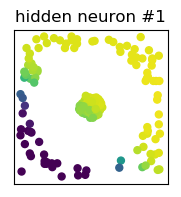
\includegraphics[width=1.6cm]{mfp/learning_process/h_neuron_5_1.png}}; 
\node (hidden1) at (1.0,3.0) {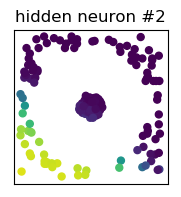
\includegraphics[width=1.6cm]{mfp/learning_process/h_neuron_5_2.png}}; 
\node (hidden2) at (2.0,3.0) {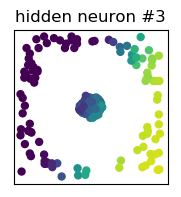
\includegraphics[width=1.6cm]{mfp/learning_process/h_neuron_5_3.png}}; 
\node (hidden3) at (3.0,3.0) {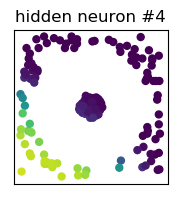
\includegraphics[width=1.6cm]{mfp/learning_process/h_neuron_5_4.png}}; 
\node (hidden4) at (4.0,3.0) {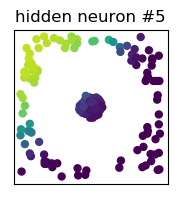
\includegraphics[width=1.6cm]{mfp/learning_process/h_neuron_5_5.png}}; 
\node (hidden5) at (5.0,3.0) {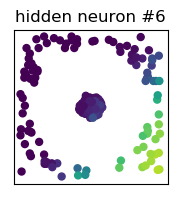
\includegraphics[width=1.6cm]{mfp/learning_process/h_neuron_5_6.png}}; 
\node (hidden6) at (6.0,3.0) {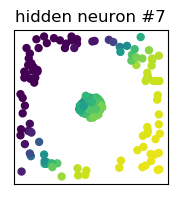
\includegraphics[width=1.6cm]{mfp/learning_process/h_neuron_5_7.png}}; 
\node (hidden7) at (7.0,3.0) {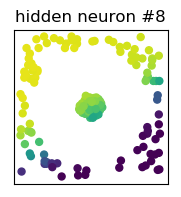
\includegraphics[width=1.6cm]{mfp/learning_process/h_neuron_5_8.png}}; 
\node (hidden8) at (8.0,3.0) {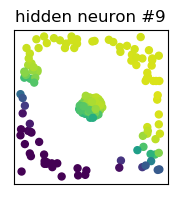
\includegraphics[width=1.6cm]{mfp/learning_process/h_neuron_5_9.png}}; 
\node (hidden9) at (9.0,3.0) {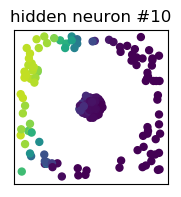
\includegraphics[width=1.6cm]{mfp/learning_process/h_neuron_5_10.png}}; 
\node (hidden10) at (10.0,3.0) {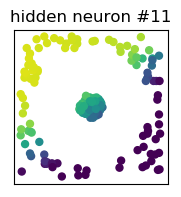
\includegraphics[width=1.6cm]{mfp/learning_process/h_neuron_5_11.png}}; 
\node (out5) at (5.2,0.0) {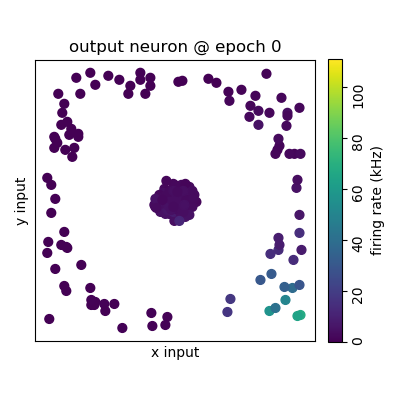
\includegraphics[width=3.6cm]{mfp/learning_process/output_neuron_5.png}}; 

\draw[-stealth,line width=0.4pt, color=red ] (hidden0.south) -- (out5); 
\draw[-stealth,line width=2.0pt, color=blue ] (hidden1.south) -- (out5); 
\draw[-stealth,line width=1.9pt, color=red ] (hidden2.south) -- (out5); 
\draw[-stealth,line width=1.1pt, color=red ] (hidden3.south) -- (out5); 
\draw[-stealth,line width=2.1pt, color=red ] (hidden4.south) -- (out5); 
\draw[-stealth,line width=2.2pt, color=red ] (hidden5.south) -- (out5); 
\draw[-stealth,line width=1.4pt, color=red ] (hidden6.south) -- (out5); 
\draw[-stealth,line width=0.1pt, color=red ] (hidden7.south) -- (out5); 
\draw[-stealth,line width=2.2pt, color=blue ] (hidden8.south) -- (out5); 
\draw[-stealth,line width=0.7pt, color=red ] (hidden9.south) -- (out5); 
\draw[-stealth,line width=0.7pt, color=red ] (hidden10.south) -- (out5); 
\end{tikzpicture} 
	\caption[Initial state of the deep network.]{Initial state of the deep network. For simplicity only the hidden and output layer are displayed. The arrows connecting the hidden units with output units resemble the synaptic connections, with red being an excitatory synapse and the thickness of the arrow corresponding to the synaptic strength.}
	\label{learning_process_s5}
\end{figure}

At the beginning of the training process, each hidden unit is initialized with linear a combination of the input schemes from \cref{circlesinputs} which is then transformed into a non-linear output by the activation function. The new representations of the input layer are again linearly combined into a net input for the output unit where another non-linear transformation is applied. The initial state of the network is shown in \cref{learning_process_s5}. At this stage of the training process the output unit cannot classify the task correctly. 

%\begin{figure}
%	\label{learning_process_s500}
%	\begin{tikzpicture}[scale=1.4] 
\node (hidden0) at (0.0,3.0) {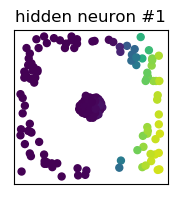
\includegraphics[width=1.6cm]{mfp/learning_process/h_neuron_500_1.png}}; 
\node (hidden1) at (1.0,3.0) {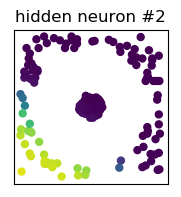
\includegraphics[width=1.6cm]{mfp/learning_process/h_neuron_500_2.png}}; 
\node (hidden2) at (2.0,3.0) {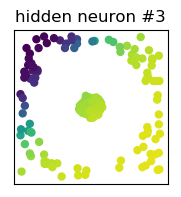
\includegraphics[width=1.6cm]{mfp/learning_process/h_neuron_500_3.png}}; 
\node (hidden3) at (3.0,3.0) {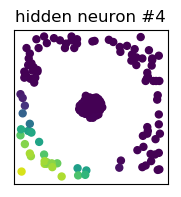
\includegraphics[width=1.6cm]{mfp/learning_process/h_neuron_500_4.png}}; 
\node (hidden4) at (4.0,3.0) {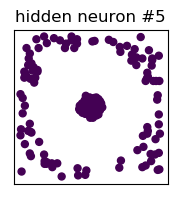
\includegraphics[width=1.6cm]{mfp/learning_process/h_neuron_500_5.png}}; 
\node (hidden5) at (5.0,3.0) {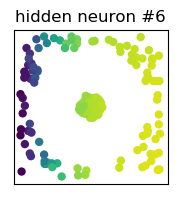
\includegraphics[width=1.6cm]{mfp/learning_process/h_neuron_500_6.png}}; 
\node (hidden6) at (6.0,3.0) {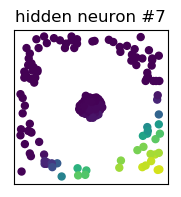
\includegraphics[width=1.6cm]{mfp/learning_process/h_neuron_500_7.png}}; 
\node (hidden7) at (7.0,3.0) {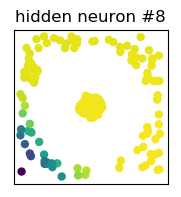
\includegraphics[width=1.6cm]{mfp/learning_process/h_neuron_500_8.png}}; 
\node (hidden8) at (8.0,3.0) {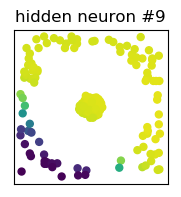
\includegraphics[width=1.6cm]{mfp/learning_process/h_neuron_500_9.png}}; 
\node (hidden9) at (9.0,3.0) {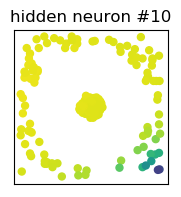
\includegraphics[width=1.6cm]{mfp/learning_process/h_neuron_500_10.png}}; 
\node (hidden10) at (10.0,3.0) {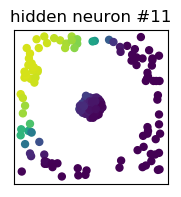
\includegraphics[width=1.6cm]{mfp/learning_process/h_neuron_500_11.png}}; 
\node (out500) at (5.2,0.0) {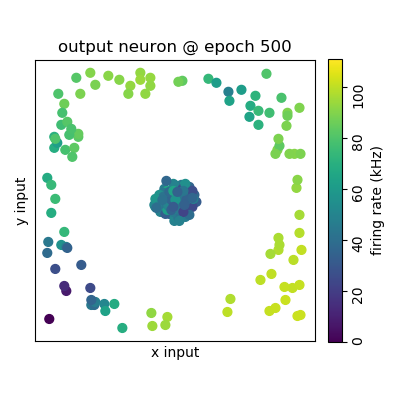
\includegraphics[width=3.6cm]{mfp/learning_process/output_neuron_500.png}}; 

\draw[-stealth,line width=1.5pt, color=red ] (hidden0.south) -- (out500); 
\draw[-stealth,line width=0.1pt, color=blue ] (hidden1.south) -- (out500); 
\draw[-stealth,line width=0.8pt, color=red ] (hidden2.south) -- (out500); 
\draw[-stealth,line width=0.7pt, color=red ] (hidden3.south) -- (out500); 
\draw[-stealth,line width=1.2pt, color=red ] (hidden4.south) -- (out500); 
\draw[-stealth,line width=2.0pt, color=red ] (hidden5.south) -- (out500); 
\draw[-stealth,line width=2.3pt, color=red ] (hidden6.south) -- (out500); 
\draw[-stealth,line width=0.9pt, color=red ] (hidden7.south) -- (out500); 
\draw[-stealth,line width=0.5pt, color=blue ] (hidden8.south) -- (out500); 
\draw[-stealth,line width=0.2pt, color=red ] (hidden9.south) -- (out500); 
\draw[-stealth,line width=2.2pt, color=red ] (hidden10.south) -- (out500); 
\end{tikzpicture} 
%	\caption[Network state after 500 iterations.]{Network state after 500 iterations. With a decision boundary of roughly \SI{60}{\kilo \Hz}, the output unit starts to correctly identify the two classes.}
%\end{figure}

The evolved network after 500 iterations is depicted in \cref{learning_process_s500} and shows first signs of improvement. The \gls{rmse} has already been cut in half and also the accuracy has improved as shown in \cref{circles_acc}. Less useful representation in the hidden layer are further modified by changing the bias or the weights. The beneficial ones are rewarded with a stronger connection to the output layer and further refinement of their bias and input weights.

At 2500 iterations, see \cref{learning_process_s2500}, the network has converged. The accuracy has also stabilized at almost 100 \%. The average over the last 500 iterations yields an mean accuracy of $(98.2 \pm 2.9)\,\%$ and the average over last 250 iterations improves to  $(99.6 \pm 0.8)\,\%$. The \gls{rmse} is also reduced to a minimum, i.e. the output neuron resembles the target well. The average output error over the last 250 iterations yields $(9.6 \pm 1.4)\,\si{\kilo \Hz}$.

\begin{figure}
	\begin{subfigure}{\textwidth}
		\caption{}
		\centering
		\begin{tikzpicture}[scale=1.4] 
\node (hidden0) at (0.0,3.0) {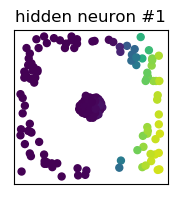
\includegraphics[width=1.6cm]{mfp/learning_process/h_neuron_500_1.png}}; 
\node (hidden1) at (1.0,3.0) {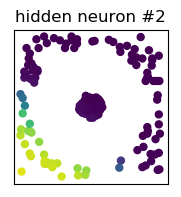
\includegraphics[width=1.6cm]{mfp/learning_process/h_neuron_500_2.png}}; 
\node (hidden2) at (2.0,3.0) {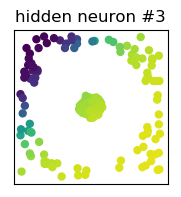
\includegraphics[width=1.6cm]{mfp/learning_process/h_neuron_500_3.png}}; 
\node (hidden3) at (3.0,3.0) {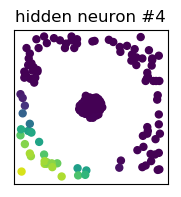
\includegraphics[width=1.6cm]{mfp/learning_process/h_neuron_500_4.png}}; 
\node (hidden4) at (4.0,3.0) {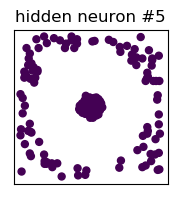
\includegraphics[width=1.6cm]{mfp/learning_process/h_neuron_500_5.png}}; 
\node (hidden5) at (5.0,3.0) {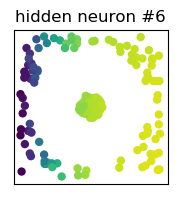
\includegraphics[width=1.6cm]{mfp/learning_process/h_neuron_500_6.png}}; 
\node (hidden6) at (6.0,3.0) {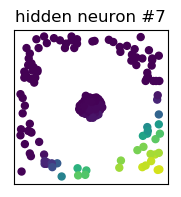
\includegraphics[width=1.6cm]{mfp/learning_process/h_neuron_500_7.png}}; 
\node (hidden7) at (7.0,3.0) {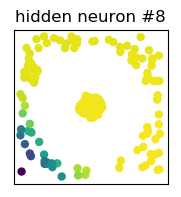
\includegraphics[width=1.6cm]{mfp/learning_process/h_neuron_500_8.png}}; 
\node (hidden8) at (8.0,3.0) {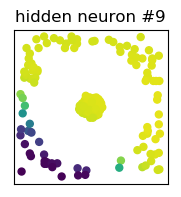
\includegraphics[width=1.6cm]{mfp/learning_process/h_neuron_500_9.png}}; 
\node (hidden9) at (9.0,3.0) {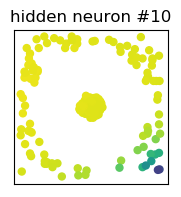
\includegraphics[width=1.6cm]{mfp/learning_process/h_neuron_500_10.png}}; 
\node (hidden10) at (10.0,3.0) {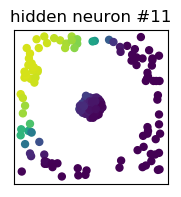
\includegraphics[width=1.6cm]{mfp/learning_process/h_neuron_500_11.png}}; 
\node (out500) at (5.2,0.0) {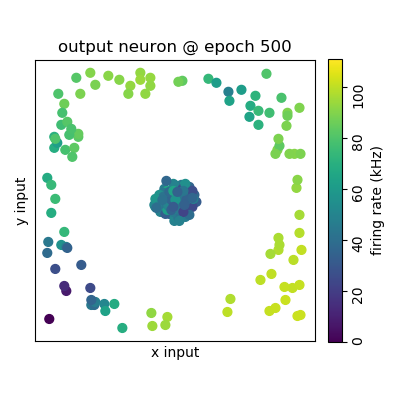
\includegraphics[width=3.6cm]{mfp/learning_process/output_neuron_500.png}}; 

\draw[-stealth,line width=1.5pt, color=red ] (hidden0.south) -- (out500); 
\draw[-stealth,line width=0.1pt, color=blue ] (hidden1.south) -- (out500); 
\draw[-stealth,line width=0.8pt, color=red ] (hidden2.south) -- (out500); 
\draw[-stealth,line width=0.7pt, color=red ] (hidden3.south) -- (out500); 
\draw[-stealth,line width=1.2pt, color=red ] (hidden4.south) -- (out500); 
\draw[-stealth,line width=2.0pt, color=red ] (hidden5.south) -- (out500); 
\draw[-stealth,line width=2.3pt, color=red ] (hidden6.south) -- (out500); 
\draw[-stealth,line width=0.9pt, color=red ] (hidden7.south) -- (out500); 
\draw[-stealth,line width=0.5pt, color=blue ] (hidden8.south) -- (out500); 
\draw[-stealth,line width=0.2pt, color=red ] (hidden9.south) -- (out500); 
\draw[-stealth,line width=2.2pt, color=red ] (hidden10.south) -- (out500); 
\end{tikzpicture} 
		\label{learning_process_s500}
	\end{subfigure}
	\begin{subfigure}{\textwidth}
		\caption{}
		\centering
		\begin{tikzpicture}[scale=1.4] 
\node (hidden0) at (0.0,3.0) {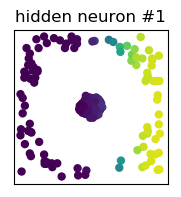
\includegraphics[width=1.6cm]{mfp/learning_process/h_neuron_2500_1.png}}; 
\node (hidden1) at (1.0,3.0) {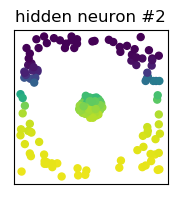
\includegraphics[width=1.6cm]{mfp/learning_process/h_neuron_2500_2.png}}; 
\node (hidden2) at (2.0,3.0) {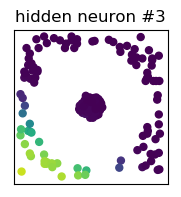
\includegraphics[width=1.6cm]{mfp/learning_process/h_neuron_2500_3.png}}; 
\node (hidden3) at (3.0,3.0) {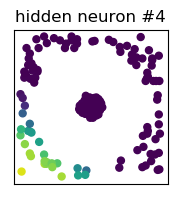
\includegraphics[width=1.6cm]{mfp/learning_process/h_neuron_2500_4.png}}; 
\node (hidden4) at (4.0,3.0) {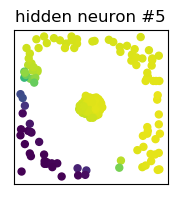
\includegraphics[width=1.6cm]{mfp/learning_process/h_neuron_2500_5.png}}; 
\node (hidden5) at (5.0,3.0) {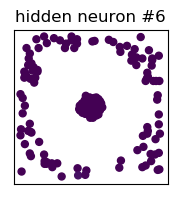
\includegraphics[width=1.6cm]{mfp/learning_process/h_neuron_2500_6.png}}; 
\node (hidden6) at (6.0,3.0) {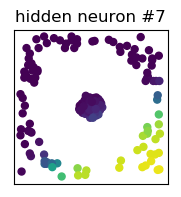
\includegraphics[width=1.6cm]{mfp/learning_process/h_neuron_2500_7.png}}; 
\node (hidden7) at (7.0,3.0) {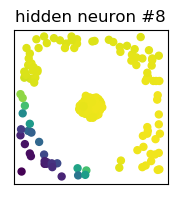
\includegraphics[width=1.6cm]{mfp/learning_process/h_neuron_2500_8.png}}; 
\node (hidden8) at (8.0,3.0) {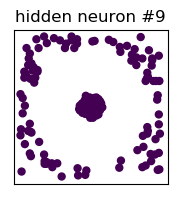
\includegraphics[width=1.6cm]{mfp/learning_process/h_neuron_2500_9.png}}; 
\node (hidden9) at (9.0,3.0) {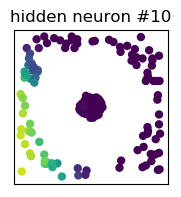
\includegraphics[width=1.6cm]{mfp/learning_process/h_neuron_2500_10.png}}; 
\node (hidden10) at (10.0,3.0) {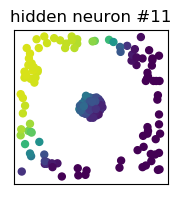
\includegraphics[width=1.6cm]{mfp/learning_process/h_neuron_2500_11.png}}; 
\node (out5) at (5.2,0.0) {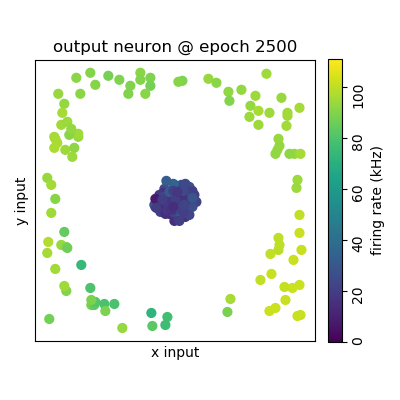
\includegraphics[width=3.6cm]{mfp/learning_process/output_neuron_2500.png}}; 

\draw[-stealth,line width=0.4pt, color=red ] (hidden0.south) -- (out5); 
\draw[-stealth,line width=2.0pt, color=blue ] (hidden1.south) -- (out5); 
\draw[-stealth,line width=1.9pt, color=red ] (hidden2.south) -- (out5); 
\draw[-stealth,line width=1.1pt, color=red ] (hidden3.south) -- (out5); 
\draw[-stealth,line width=2.1pt, color=red ] (hidden4.south) -- (out5); 
\draw[-stealth,line width=2.2pt, color=red ] (hidden5.south) -- (out5); 
\draw[-stealth,line width=1.4pt, color=red ] (hidden6.south) -- (out5); 
\draw[-stealth,line width=0.1pt, color=red ] (hidden7.south) -- (out5); 
\draw[-stealth,line width=2.2pt, color=blue ] (hidden8.south) -- (out5); 
\draw[-stealth,line width=0.7pt, color=red ] (hidden9.south) -- (out5); 
\draw[-stealth,line width=0.7pt, color=red ] (hidden10.south) -- (out5); 
\end{tikzpicture} 
		\label{learning_process_s2500}
	\end{subfigure}
	\caption[Evolution of the network during training.]{Evolution of the network during training. \textbf{(\subref{learning_process_s500})} Network state after 500 iterations. With a decision boundary of roughly \SI{60}{\kilo \Hz}, the output unit starts to correctly identify the two classes. \textbf{(\subref{learning_process_s2500})} Final trained state of the network. After 2500 iterations the network has succeed to separate both classes with a accuracy of almost 100 \%.}
\end{figure}

%For further monitoring purposes, the evolution of the weights and biases are tracked for the hidden and output layer (see \cref{network_monitoring}).
%\begin{figure}
%	\centering
%    %% Creator: Matplotlib, PGF backend
%%
%% To include the figure in your LaTeX document, write
%%   \input{<filename>.pgf}
%%
%% Make sure the required packages are loaded in your preamble
%%   \usepackage{pgf}
%%
%% Figures using additional raster images can only be included by \input if
%% they are in the same directory as the main LaTeX file. For loading figures
%% from other directories you can use the `import` package
%%   \usepackage{import}
%% and then include the figures with
%%   \import{<path to file>}{<filename>.pgf}
%%
%% Matplotlib used the following preamble
%%   \usepackage{amsmath} \usepackage{pifont} \usepackage{xcolor} \definecolor{green}{HTML}{467821} \definecolor{red}{HTML}{CF4457} \usepackage[detect-all]{siunitx}
%%   \usepackage{fontspec}
%%
\begingroup%
\makeatletter%
\begin{pgfpicture}%
\pgfpathrectangle{\pgfpointorigin}{\pgfqpoint{6.138952in}{2.778545in}}%
\pgfusepath{use as bounding box, clip}%
\begin{pgfscope}%
\pgfsetbuttcap%
\pgfsetmiterjoin%
\pgfsetlinewidth{0.000000pt}%
\definecolor{currentstroke}{rgb}{0.000000,0.000000,0.000000}%
\pgfsetstrokecolor{currentstroke}%
\pgfsetstrokeopacity{0.000000}%
\pgfsetdash{}{0pt}%
\pgfpathmoveto{\pgfqpoint{0.000000in}{0.000000in}}%
\pgfpathlineto{\pgfqpoint{6.138952in}{0.000000in}}%
\pgfpathlineto{\pgfqpoint{6.138952in}{2.778545in}}%
\pgfpathlineto{\pgfqpoint{0.000000in}{2.778545in}}%
\pgfpathclose%
\pgfusepath{}%
\end{pgfscope}%
\begin{pgfscope}%
\pgfsetbuttcap%
\pgfsetmiterjoin%
\pgfsetlinewidth{0.000000pt}%
\definecolor{currentstroke}{rgb}{0.000000,0.000000,0.000000}%
\pgfsetstrokecolor{currentstroke}%
\pgfsetstrokeopacity{0.000000}%
\pgfsetdash{}{0pt}%
\pgfpathmoveto{\pgfqpoint{0.488751in}{1.551716in}}%
\pgfpathlineto{\pgfqpoint{2.749168in}{1.551716in}}%
\pgfpathlineto{\pgfqpoint{2.749168in}{2.678545in}}%
\pgfpathlineto{\pgfqpoint{0.488751in}{2.678545in}}%
\pgfpathclose%
\pgfusepath{}%
\end{pgfscope}%
\begin{pgfscope}%
\pgfsetbuttcap%
\pgfsetroundjoin%
\definecolor{currentfill}{rgb}{0.317647,0.317647,0.317647}%
\pgfsetfillcolor{currentfill}%
\pgfsetlinewidth{0.501875pt}%
\definecolor{currentstroke}{rgb}{0.317647,0.317647,0.317647}%
\pgfsetstrokecolor{currentstroke}%
\pgfsetdash{}{0pt}%
\pgfsys@defobject{currentmarker}{\pgfqpoint{0.000000in}{-0.020833in}}{\pgfqpoint{0.000000in}{0.000000in}}{%
\pgfpathmoveto{\pgfqpoint{0.000000in}{0.000000in}}%
\pgfpathlineto{\pgfqpoint{0.000000in}{-0.020833in}}%
\pgfusepath{stroke,fill}%
}%
\begin{pgfscope}%
\pgfsys@transformshift{0.591497in}{1.551716in}%
\pgfsys@useobject{currentmarker}{}%
\end{pgfscope}%
\end{pgfscope}%
\begin{pgfscope}%
\pgfsetbuttcap%
\pgfsetroundjoin%
\definecolor{currentfill}{rgb}{0.317647,0.317647,0.317647}%
\pgfsetfillcolor{currentfill}%
\pgfsetlinewidth{0.501875pt}%
\definecolor{currentstroke}{rgb}{0.317647,0.317647,0.317647}%
\pgfsetstrokecolor{currentstroke}%
\pgfsetdash{}{0pt}%
\pgfsys@defobject{currentmarker}{\pgfqpoint{0.000000in}{-0.020833in}}{\pgfqpoint{0.000000in}{0.000000in}}{%
\pgfpathmoveto{\pgfqpoint{0.000000in}{0.000000in}}%
\pgfpathlineto{\pgfqpoint{0.000000in}{-0.020833in}}%
\pgfusepath{stroke,fill}%
}%
\begin{pgfscope}%
\pgfsys@transformshift{1.003306in}{1.551716in}%
\pgfsys@useobject{currentmarker}{}%
\end{pgfscope}%
\end{pgfscope}%
\begin{pgfscope}%
\pgfsetbuttcap%
\pgfsetroundjoin%
\definecolor{currentfill}{rgb}{0.317647,0.317647,0.317647}%
\pgfsetfillcolor{currentfill}%
\pgfsetlinewidth{0.501875pt}%
\definecolor{currentstroke}{rgb}{0.317647,0.317647,0.317647}%
\pgfsetstrokecolor{currentstroke}%
\pgfsetdash{}{0pt}%
\pgfsys@defobject{currentmarker}{\pgfqpoint{0.000000in}{-0.020833in}}{\pgfqpoint{0.000000in}{0.000000in}}{%
\pgfpathmoveto{\pgfqpoint{0.000000in}{0.000000in}}%
\pgfpathlineto{\pgfqpoint{0.000000in}{-0.020833in}}%
\pgfusepath{stroke,fill}%
}%
\begin{pgfscope}%
\pgfsys@transformshift{1.415114in}{1.551716in}%
\pgfsys@useobject{currentmarker}{}%
\end{pgfscope}%
\end{pgfscope}%
\begin{pgfscope}%
\pgfsetbuttcap%
\pgfsetroundjoin%
\definecolor{currentfill}{rgb}{0.317647,0.317647,0.317647}%
\pgfsetfillcolor{currentfill}%
\pgfsetlinewidth{0.501875pt}%
\definecolor{currentstroke}{rgb}{0.317647,0.317647,0.317647}%
\pgfsetstrokecolor{currentstroke}%
\pgfsetdash{}{0pt}%
\pgfsys@defobject{currentmarker}{\pgfqpoint{0.000000in}{-0.020833in}}{\pgfqpoint{0.000000in}{0.000000in}}{%
\pgfpathmoveto{\pgfqpoint{0.000000in}{0.000000in}}%
\pgfpathlineto{\pgfqpoint{0.000000in}{-0.020833in}}%
\pgfusepath{stroke,fill}%
}%
\begin{pgfscope}%
\pgfsys@transformshift{1.826922in}{1.551716in}%
\pgfsys@useobject{currentmarker}{}%
\end{pgfscope}%
\end{pgfscope}%
\begin{pgfscope}%
\pgfsetbuttcap%
\pgfsetroundjoin%
\definecolor{currentfill}{rgb}{0.317647,0.317647,0.317647}%
\pgfsetfillcolor{currentfill}%
\pgfsetlinewidth{0.501875pt}%
\definecolor{currentstroke}{rgb}{0.317647,0.317647,0.317647}%
\pgfsetstrokecolor{currentstroke}%
\pgfsetdash{}{0pt}%
\pgfsys@defobject{currentmarker}{\pgfqpoint{0.000000in}{-0.020833in}}{\pgfqpoint{0.000000in}{0.000000in}}{%
\pgfpathmoveto{\pgfqpoint{0.000000in}{0.000000in}}%
\pgfpathlineto{\pgfqpoint{0.000000in}{-0.020833in}}%
\pgfusepath{stroke,fill}%
}%
\begin{pgfscope}%
\pgfsys@transformshift{2.238731in}{1.551716in}%
\pgfsys@useobject{currentmarker}{}%
\end{pgfscope}%
\end{pgfscope}%
\begin{pgfscope}%
\pgfsetbuttcap%
\pgfsetroundjoin%
\definecolor{currentfill}{rgb}{0.317647,0.317647,0.317647}%
\pgfsetfillcolor{currentfill}%
\pgfsetlinewidth{0.501875pt}%
\definecolor{currentstroke}{rgb}{0.317647,0.317647,0.317647}%
\pgfsetstrokecolor{currentstroke}%
\pgfsetdash{}{0pt}%
\pgfsys@defobject{currentmarker}{\pgfqpoint{0.000000in}{-0.020833in}}{\pgfqpoint{0.000000in}{0.000000in}}{%
\pgfpathmoveto{\pgfqpoint{0.000000in}{0.000000in}}%
\pgfpathlineto{\pgfqpoint{0.000000in}{-0.020833in}}%
\pgfusepath{stroke,fill}%
}%
\begin{pgfscope}%
\pgfsys@transformshift{2.650539in}{1.551716in}%
\pgfsys@useobject{currentmarker}{}%
\end{pgfscope}%
\end{pgfscope}%
\begin{pgfscope}%
\pgfsetbuttcap%
\pgfsetroundjoin%
\definecolor{currentfill}{rgb}{0.317647,0.317647,0.317647}%
\pgfsetfillcolor{currentfill}%
\pgfsetlinewidth{0.501875pt}%
\definecolor{currentstroke}{rgb}{0.317647,0.317647,0.317647}%
\pgfsetstrokecolor{currentstroke}%
\pgfsetdash{}{0pt}%
\pgfsys@defobject{currentmarker}{\pgfqpoint{-0.020833in}{0.000000in}}{\pgfqpoint{0.000000in}{0.000000in}}{%
\pgfpathmoveto{\pgfqpoint{0.000000in}{0.000000in}}%
\pgfpathlineto{\pgfqpoint{-0.020833in}{0.000000in}}%
\pgfusepath{stroke,fill}%
}%
\begin{pgfscope}%
\pgfsys@transformshift{0.488751in}{1.788066in}%
\pgfsys@useobject{currentmarker}{}%
\end{pgfscope}%
\end{pgfscope}%
\begin{pgfscope}%
\definecolor{textcolor}{rgb}{0.317647,0.317647,0.317647}%
\pgfsetstrokecolor{textcolor}%
\pgfsetfillcolor{textcolor}%
\pgftext[x=0.256497in,y=1.755949in,left,base]{\color{textcolor}\rmfamily\fontsize{6.664000}{7.996800}\selectfont \(\displaystyle -20\)}%
\end{pgfscope}%
\begin{pgfscope}%
\pgfsetbuttcap%
\pgfsetroundjoin%
\definecolor{currentfill}{rgb}{0.317647,0.317647,0.317647}%
\pgfsetfillcolor{currentfill}%
\pgfsetlinewidth{0.501875pt}%
\definecolor{currentstroke}{rgb}{0.317647,0.317647,0.317647}%
\pgfsetstrokecolor{currentstroke}%
\pgfsetdash{}{0pt}%
\pgfsys@defobject{currentmarker}{\pgfqpoint{-0.020833in}{0.000000in}}{\pgfqpoint{0.000000in}{0.000000in}}{%
\pgfpathmoveto{\pgfqpoint{0.000000in}{0.000000in}}%
\pgfpathlineto{\pgfqpoint{-0.020833in}{0.000000in}}%
\pgfusepath{stroke,fill}%
}%
\begin{pgfscope}%
\pgfsys@transformshift{0.488751in}{2.034907in}%
\pgfsys@useobject{currentmarker}{}%
\end{pgfscope}%
\end{pgfscope}%
\begin{pgfscope}%
\definecolor{textcolor}{rgb}{0.317647,0.317647,0.317647}%
\pgfsetstrokecolor{textcolor}%
\pgfsetfillcolor{textcolor}%
\pgftext[x=0.398666in,y=2.002790in,left,base]{\color{textcolor}\rmfamily\fontsize{6.664000}{7.996800}\selectfont \(\displaystyle 0\)}%
\end{pgfscope}%
\begin{pgfscope}%
\pgfsetbuttcap%
\pgfsetroundjoin%
\definecolor{currentfill}{rgb}{0.317647,0.317647,0.317647}%
\pgfsetfillcolor{currentfill}%
\pgfsetlinewidth{0.501875pt}%
\definecolor{currentstroke}{rgb}{0.317647,0.317647,0.317647}%
\pgfsetstrokecolor{currentstroke}%
\pgfsetdash{}{0pt}%
\pgfsys@defobject{currentmarker}{\pgfqpoint{-0.020833in}{0.000000in}}{\pgfqpoint{0.000000in}{0.000000in}}{%
\pgfpathmoveto{\pgfqpoint{0.000000in}{0.000000in}}%
\pgfpathlineto{\pgfqpoint{-0.020833in}{0.000000in}}%
\pgfusepath{stroke,fill}%
}%
\begin{pgfscope}%
\pgfsys@transformshift{0.488751in}{2.281748in}%
\pgfsys@useobject{currentmarker}{}%
\end{pgfscope}%
\end{pgfscope}%
\begin{pgfscope}%
\definecolor{textcolor}{rgb}{0.317647,0.317647,0.317647}%
\pgfsetstrokecolor{textcolor}%
\pgfsetfillcolor{textcolor}%
\pgftext[x=0.343303in,y=2.249631in,left,base]{\color{textcolor}\rmfamily\fontsize{6.664000}{7.996800}\selectfont \(\displaystyle 20\)}%
\end{pgfscope}%
\begin{pgfscope}%
\pgfsetbuttcap%
\pgfsetroundjoin%
\definecolor{currentfill}{rgb}{0.317647,0.317647,0.317647}%
\pgfsetfillcolor{currentfill}%
\pgfsetlinewidth{0.501875pt}%
\definecolor{currentstroke}{rgb}{0.317647,0.317647,0.317647}%
\pgfsetstrokecolor{currentstroke}%
\pgfsetdash{}{0pt}%
\pgfsys@defobject{currentmarker}{\pgfqpoint{-0.020833in}{0.000000in}}{\pgfqpoint{0.000000in}{0.000000in}}{%
\pgfpathmoveto{\pgfqpoint{0.000000in}{0.000000in}}%
\pgfpathlineto{\pgfqpoint{-0.020833in}{0.000000in}}%
\pgfusepath{stroke,fill}%
}%
\begin{pgfscope}%
\pgfsys@transformshift{0.488751in}{2.528589in}%
\pgfsys@useobject{currentmarker}{}%
\end{pgfscope}%
\end{pgfscope}%
\begin{pgfscope}%
\definecolor{textcolor}{rgb}{0.317647,0.317647,0.317647}%
\pgfsetstrokecolor{textcolor}%
\pgfsetfillcolor{textcolor}%
\pgftext[x=0.343303in,y=2.496472in,left,base]{\color{textcolor}\rmfamily\fontsize{6.664000}{7.996800}\selectfont \(\displaystyle 40\)}%
\end{pgfscope}%
\begin{pgfscope}%
\definecolor{textcolor}{rgb}{0.317647,0.317647,0.317647}%
\pgfsetstrokecolor{textcolor}%
\pgfsetfillcolor{textcolor}%
\pgftext[x=0.200942in,y=2.115130in,,bottom,rotate=90.000000]{\color{textcolor}\rmfamily\fontsize{6.664000}{7.996800}\selectfont \(\displaystyle W^{(\mathrm{h})}\)}%
\end{pgfscope}%
\begin{pgfscope}%
\pgfpathrectangle{\pgfqpoint{0.488751in}{1.551716in}}{\pgfqpoint{2.260417in}{1.126829in}}%
\pgfusepath{clip}%
\pgfsetrectcap%
\pgfsetroundjoin%
\pgfsetlinewidth{0.803000pt}%
\definecolor{currentstroke}{rgb}{0.333333,0.333333,0.333333}%
\pgfsetstrokecolor{currentstroke}%
\pgfsetdash{}{0pt}%
\pgfpathmoveto{\pgfqpoint{0.591497in}{2.294090in}}%
\pgfpathlineto{\pgfqpoint{0.595615in}{2.331116in}}%
\pgfpathlineto{\pgfqpoint{0.599733in}{2.331116in}}%
\pgfpathlineto{\pgfqpoint{0.603851in}{2.318774in}}%
\pgfpathlineto{\pgfqpoint{0.612087in}{2.405169in}}%
\pgfpathlineto{\pgfqpoint{0.616206in}{2.380484in}}%
\pgfpathlineto{\pgfqpoint{0.620324in}{2.368142in}}%
\pgfpathlineto{\pgfqpoint{0.624442in}{2.368142in}}%
\pgfpathlineto{\pgfqpoint{0.628560in}{2.417511in}}%
\pgfpathlineto{\pgfqpoint{0.636796in}{2.417511in}}%
\pgfpathlineto{\pgfqpoint{0.640914in}{2.405169in}}%
\pgfpathlineto{\pgfqpoint{0.645032in}{2.454537in}}%
\pgfpathlineto{\pgfqpoint{0.649150in}{2.442195in}}%
\pgfpathlineto{\pgfqpoint{0.653268in}{2.392827in}}%
\pgfpathlineto{\pgfqpoint{0.657386in}{2.417511in}}%
\pgfpathlineto{\pgfqpoint{0.661504in}{2.454537in}}%
\pgfpathlineto{\pgfqpoint{0.665623in}{2.479221in}}%
\pgfpathlineto{\pgfqpoint{0.669741in}{2.380484in}}%
\pgfpathlineto{\pgfqpoint{0.673859in}{2.392827in}}%
\pgfpathlineto{\pgfqpoint{0.682095in}{2.318774in}}%
\pgfpathlineto{\pgfqpoint{0.686213in}{2.331116in}}%
\pgfpathlineto{\pgfqpoint{0.690331in}{2.306432in}}%
\pgfpathlineto{\pgfqpoint{0.694449in}{2.306432in}}%
\pgfpathlineto{\pgfqpoint{0.706803in}{2.269406in}}%
\pgfpathlineto{\pgfqpoint{0.710922in}{2.281748in}}%
\pgfpathlineto{\pgfqpoint{0.715040in}{2.257064in}}%
\pgfpathlineto{\pgfqpoint{0.719158in}{2.269406in}}%
\pgfpathlineto{\pgfqpoint{0.723276in}{2.257064in}}%
\pgfpathlineto{\pgfqpoint{0.727394in}{2.257064in}}%
\pgfpathlineto{\pgfqpoint{0.731512in}{2.269406in}}%
\pgfpathlineto{\pgfqpoint{0.739748in}{2.269406in}}%
\pgfpathlineto{\pgfqpoint{0.743866in}{2.281748in}}%
\pgfpathlineto{\pgfqpoint{0.747984in}{2.257064in}}%
\pgfpathlineto{\pgfqpoint{0.768575in}{2.257064in}}%
\pgfpathlineto{\pgfqpoint{0.772693in}{2.269406in}}%
\pgfpathlineto{\pgfqpoint{0.776811in}{2.269406in}}%
\pgfpathlineto{\pgfqpoint{0.785047in}{2.244722in}}%
\pgfpathlineto{\pgfqpoint{0.789165in}{2.257064in}}%
\pgfpathlineto{\pgfqpoint{0.805637in}{2.257064in}}%
\pgfpathlineto{\pgfqpoint{0.809756in}{2.294090in}}%
\pgfpathlineto{\pgfqpoint{0.813874in}{2.306432in}}%
\pgfpathlineto{\pgfqpoint{0.822110in}{2.306432in}}%
\pgfpathlineto{\pgfqpoint{0.826228in}{2.294090in}}%
\pgfpathlineto{\pgfqpoint{0.830346in}{2.269406in}}%
\pgfpathlineto{\pgfqpoint{0.834464in}{2.269406in}}%
\pgfpathlineto{\pgfqpoint{0.838582in}{2.294090in}}%
\pgfpathlineto{\pgfqpoint{0.842700in}{2.294090in}}%
\pgfpathlineto{\pgfqpoint{0.846818in}{2.306432in}}%
\pgfpathlineto{\pgfqpoint{0.850936in}{2.331116in}}%
\pgfpathlineto{\pgfqpoint{0.855054in}{2.318774in}}%
\pgfpathlineto{\pgfqpoint{0.883881in}{2.318774in}}%
\pgfpathlineto{\pgfqpoint{0.892117in}{2.343458in}}%
\pgfpathlineto{\pgfqpoint{0.896235in}{2.318774in}}%
\pgfpathlineto{\pgfqpoint{0.900353in}{2.343458in}}%
\pgfpathlineto{\pgfqpoint{0.904471in}{2.355800in}}%
\pgfpathlineto{\pgfqpoint{0.908590in}{2.355800in}}%
\pgfpathlineto{\pgfqpoint{0.912708in}{2.343458in}}%
\pgfpathlineto{\pgfqpoint{0.916826in}{2.343458in}}%
\pgfpathlineto{\pgfqpoint{0.920944in}{2.355800in}}%
\pgfpathlineto{\pgfqpoint{0.925062in}{2.355800in}}%
\pgfpathlineto{\pgfqpoint{0.933298in}{2.331116in}}%
\pgfpathlineto{\pgfqpoint{0.937416in}{2.331116in}}%
\pgfpathlineto{\pgfqpoint{0.941534in}{2.318774in}}%
\pgfpathlineto{\pgfqpoint{0.978597in}{2.318774in}}%
\pgfpathlineto{\pgfqpoint{0.982715in}{2.306432in}}%
\pgfpathlineto{\pgfqpoint{0.990951in}{2.306432in}}%
\pgfpathlineto{\pgfqpoint{0.995069in}{2.294090in}}%
\pgfpathlineto{\pgfqpoint{0.999187in}{2.306432in}}%
\pgfpathlineto{\pgfqpoint{1.003306in}{2.294090in}}%
\pgfpathlineto{\pgfqpoint{1.069195in}{2.294090in}}%
\pgfpathlineto{\pgfqpoint{1.073313in}{2.306432in}}%
\pgfpathlineto{\pgfqpoint{1.081549in}{2.306432in}}%
\pgfpathlineto{\pgfqpoint{1.085667in}{2.331116in}}%
\pgfpathlineto{\pgfqpoint{1.089785in}{2.331116in}}%
\pgfpathlineto{\pgfqpoint{1.093903in}{2.318774in}}%
\pgfpathlineto{\pgfqpoint{1.110376in}{2.318774in}}%
\pgfpathlineto{\pgfqpoint{1.114494in}{2.331116in}}%
\pgfpathlineto{\pgfqpoint{1.118612in}{2.331116in}}%
\pgfpathlineto{\pgfqpoint{1.122730in}{2.318774in}}%
\pgfpathlineto{\pgfqpoint{1.126848in}{2.281748in}}%
\pgfpathlineto{\pgfqpoint{1.130966in}{2.269406in}}%
\pgfpathlineto{\pgfqpoint{1.168029in}{2.269406in}}%
\pgfpathlineto{\pgfqpoint{1.172147in}{2.281748in}}%
\pgfpathlineto{\pgfqpoint{1.180383in}{2.281748in}}%
\pgfpathlineto{\pgfqpoint{1.184501in}{2.306432in}}%
\pgfpathlineto{\pgfqpoint{1.188619in}{2.281748in}}%
\pgfpathlineto{\pgfqpoint{1.196855in}{2.281748in}}%
\pgfpathlineto{\pgfqpoint{1.200974in}{2.294090in}}%
\pgfpathlineto{\pgfqpoint{1.217446in}{2.294090in}}%
\pgfpathlineto{\pgfqpoint{1.221564in}{2.306432in}}%
\pgfpathlineto{\pgfqpoint{1.225682in}{2.306432in}}%
\pgfpathlineto{\pgfqpoint{1.229800in}{2.331116in}}%
\pgfpathlineto{\pgfqpoint{1.246273in}{2.331116in}}%
\pgfpathlineto{\pgfqpoint{1.250391in}{2.306432in}}%
\pgfpathlineto{\pgfqpoint{1.254509in}{2.306432in}}%
\pgfpathlineto{\pgfqpoint{1.258627in}{2.294090in}}%
\pgfpathlineto{\pgfqpoint{1.262745in}{2.306432in}}%
\pgfpathlineto{\pgfqpoint{1.266863in}{2.306432in}}%
\pgfpathlineto{\pgfqpoint{1.270981in}{2.318774in}}%
\pgfpathlineto{\pgfqpoint{1.303926in}{2.318774in}}%
\pgfpathlineto{\pgfqpoint{1.308044in}{2.294090in}}%
\pgfpathlineto{\pgfqpoint{1.312162in}{2.306432in}}%
\pgfpathlineto{\pgfqpoint{1.316280in}{2.306432in}}%
\pgfpathlineto{\pgfqpoint{1.320398in}{2.281748in}}%
\pgfpathlineto{\pgfqpoint{1.340988in}{2.281748in}}%
\pgfpathlineto{\pgfqpoint{1.345107in}{2.294090in}}%
\pgfpathlineto{\pgfqpoint{1.382169in}{2.294090in}}%
\pgfpathlineto{\pgfqpoint{1.394524in}{2.331116in}}%
\pgfpathlineto{\pgfqpoint{1.419232in}{2.331116in}}%
\pgfpathlineto{\pgfqpoint{1.423350in}{2.318774in}}%
\pgfpathlineto{\pgfqpoint{1.435704in}{2.318774in}}%
\pgfpathlineto{\pgfqpoint{1.439822in}{2.343458in}}%
\pgfpathlineto{\pgfqpoint{1.464531in}{2.343458in}}%
\pgfpathlineto{\pgfqpoint{1.468649in}{2.318774in}}%
\pgfpathlineto{\pgfqpoint{1.481003in}{2.318774in}}%
\pgfpathlineto{\pgfqpoint{1.489240in}{2.368142in}}%
\pgfpathlineto{\pgfqpoint{1.493358in}{2.355800in}}%
\pgfpathlineto{\pgfqpoint{1.497476in}{2.355800in}}%
\pgfpathlineto{\pgfqpoint{1.501594in}{2.343458in}}%
\pgfpathlineto{\pgfqpoint{1.509830in}{2.343458in}}%
\pgfpathlineto{\pgfqpoint{1.513948in}{2.331116in}}%
\pgfpathlineto{\pgfqpoint{1.518066in}{2.343458in}}%
\pgfpathlineto{\pgfqpoint{1.522184in}{2.343458in}}%
\pgfpathlineto{\pgfqpoint{1.530420in}{2.318774in}}%
\pgfpathlineto{\pgfqpoint{1.534538in}{2.294090in}}%
\pgfpathlineto{\pgfqpoint{1.563365in}{2.294090in}}%
\pgfpathlineto{\pgfqpoint{1.567483in}{2.306432in}}%
\pgfpathlineto{\pgfqpoint{1.579837in}{2.306432in}}%
\pgfpathlineto{\pgfqpoint{1.583955in}{2.331116in}}%
\pgfpathlineto{\pgfqpoint{1.596310in}{2.331116in}}%
\pgfpathlineto{\pgfqpoint{1.600428in}{2.306432in}}%
\pgfpathlineto{\pgfqpoint{1.604546in}{2.306432in}}%
\pgfpathlineto{\pgfqpoint{1.608664in}{2.294090in}}%
\pgfpathlineto{\pgfqpoint{1.612782in}{2.294090in}}%
\pgfpathlineto{\pgfqpoint{1.616900in}{2.281748in}}%
\pgfpathlineto{\pgfqpoint{1.621018in}{2.294090in}}%
\pgfpathlineto{\pgfqpoint{1.625136in}{2.318774in}}%
\pgfpathlineto{\pgfqpoint{1.645727in}{2.318774in}}%
\pgfpathlineto{\pgfqpoint{1.649845in}{2.331116in}}%
\pgfpathlineto{\pgfqpoint{1.658081in}{2.331116in}}%
\pgfpathlineto{\pgfqpoint{1.662199in}{2.306432in}}%
\pgfpathlineto{\pgfqpoint{1.674553in}{2.306432in}}%
\pgfpathlineto{\pgfqpoint{1.678671in}{2.331116in}}%
\pgfpathlineto{\pgfqpoint{1.682789in}{2.343458in}}%
\pgfpathlineto{\pgfqpoint{1.703380in}{2.343458in}}%
\pgfpathlineto{\pgfqpoint{1.707498in}{2.331116in}}%
\pgfpathlineto{\pgfqpoint{1.711616in}{2.306432in}}%
\pgfpathlineto{\pgfqpoint{1.715734in}{2.294090in}}%
\pgfpathlineto{\pgfqpoint{1.723970in}{2.294090in}}%
\pgfpathlineto{\pgfqpoint{1.732206in}{2.343458in}}%
\pgfpathlineto{\pgfqpoint{1.756915in}{2.343458in}}%
\pgfpathlineto{\pgfqpoint{1.761033in}{2.368142in}}%
\pgfpathlineto{\pgfqpoint{1.773387in}{2.368142in}}%
\pgfpathlineto{\pgfqpoint{1.777505in}{2.380484in}}%
\pgfpathlineto{\pgfqpoint{1.781624in}{2.380484in}}%
\pgfpathlineto{\pgfqpoint{1.785742in}{2.392827in}}%
\pgfpathlineto{\pgfqpoint{1.793978in}{2.392827in}}%
\pgfpathlineto{\pgfqpoint{1.798096in}{2.380484in}}%
\pgfpathlineto{\pgfqpoint{1.802214in}{2.392827in}}%
\pgfpathlineto{\pgfqpoint{1.814568in}{2.392827in}}%
\pgfpathlineto{\pgfqpoint{1.818686in}{2.368142in}}%
\pgfpathlineto{\pgfqpoint{1.822804in}{2.380484in}}%
\pgfpathlineto{\pgfqpoint{1.826922in}{2.368142in}}%
\pgfpathlineto{\pgfqpoint{1.847513in}{2.368142in}}%
\pgfpathlineto{\pgfqpoint{1.855749in}{2.343458in}}%
\pgfpathlineto{\pgfqpoint{1.896930in}{2.343458in}}%
\pgfpathlineto{\pgfqpoint{1.901048in}{2.318774in}}%
\pgfpathlineto{\pgfqpoint{1.917520in}{2.318774in}}%
\pgfpathlineto{\pgfqpoint{1.921638in}{2.306432in}}%
\pgfpathlineto{\pgfqpoint{1.938111in}{2.306432in}}%
\pgfpathlineto{\pgfqpoint{1.942229in}{2.294090in}}%
\pgfpathlineto{\pgfqpoint{1.946347in}{2.306432in}}%
\pgfpathlineto{\pgfqpoint{1.971055in}{2.306432in}}%
\pgfpathlineto{\pgfqpoint{1.975173in}{2.318774in}}%
\pgfpathlineto{\pgfqpoint{2.028709in}{2.318774in}}%
\pgfpathlineto{\pgfqpoint{2.032827in}{2.331116in}}%
\pgfpathlineto{\pgfqpoint{2.036945in}{2.318774in}}%
\pgfpathlineto{\pgfqpoint{2.041063in}{2.318774in}}%
\pgfpathlineto{\pgfqpoint{2.045181in}{2.294090in}}%
\pgfpathlineto{\pgfqpoint{2.061653in}{2.294090in}}%
\pgfpathlineto{\pgfqpoint{2.065771in}{2.269406in}}%
\pgfpathlineto{\pgfqpoint{2.069889in}{2.269406in}}%
\pgfpathlineto{\pgfqpoint{2.074008in}{2.257064in}}%
\pgfpathlineto{\pgfqpoint{2.168723in}{2.257064in}}%
\pgfpathlineto{\pgfqpoint{2.172842in}{2.269406in}}%
\pgfpathlineto{\pgfqpoint{2.181078in}{2.269406in}}%
\pgfpathlineto{\pgfqpoint{2.185196in}{2.306432in}}%
\pgfpathlineto{\pgfqpoint{2.189314in}{2.306432in}}%
\pgfpathlineto{\pgfqpoint{2.193432in}{2.331116in}}%
\pgfpathlineto{\pgfqpoint{2.197550in}{2.318774in}}%
\pgfpathlineto{\pgfqpoint{2.201668in}{2.355800in}}%
\pgfpathlineto{\pgfqpoint{2.205786in}{2.355800in}}%
\pgfpathlineto{\pgfqpoint{2.209904in}{2.380484in}}%
\pgfpathlineto{\pgfqpoint{2.218140in}{2.405169in}}%
\pgfpathlineto{\pgfqpoint{2.222259in}{2.392827in}}%
\pgfpathlineto{\pgfqpoint{2.226377in}{2.417511in}}%
\pgfpathlineto{\pgfqpoint{2.230495in}{2.405169in}}%
\pgfpathlineto{\pgfqpoint{2.234613in}{2.417511in}}%
\pgfpathlineto{\pgfqpoint{2.242849in}{2.392827in}}%
\pgfpathlineto{\pgfqpoint{2.259321in}{2.392827in}}%
\pgfpathlineto{\pgfqpoint{2.267557in}{2.417511in}}%
\pgfpathlineto{\pgfqpoint{2.271676in}{2.442195in}}%
\pgfpathlineto{\pgfqpoint{2.275794in}{2.454537in}}%
\pgfpathlineto{\pgfqpoint{2.279912in}{2.429853in}}%
\pgfpathlineto{\pgfqpoint{2.284030in}{2.392827in}}%
\pgfpathlineto{\pgfqpoint{2.288148in}{2.392827in}}%
\pgfpathlineto{\pgfqpoint{2.292266in}{2.417511in}}%
\pgfpathlineto{\pgfqpoint{2.296384in}{2.417511in}}%
\pgfpathlineto{\pgfqpoint{2.300502in}{2.442195in}}%
\pgfpathlineto{\pgfqpoint{2.304620in}{2.405169in}}%
\pgfpathlineto{\pgfqpoint{2.308738in}{2.417511in}}%
\pgfpathlineto{\pgfqpoint{2.325211in}{2.417511in}}%
\pgfpathlineto{\pgfqpoint{2.329329in}{2.442195in}}%
\pgfpathlineto{\pgfqpoint{2.333447in}{2.417511in}}%
\pgfpathlineto{\pgfqpoint{2.337565in}{2.417511in}}%
\pgfpathlineto{\pgfqpoint{2.345801in}{2.442195in}}%
\pgfpathlineto{\pgfqpoint{2.349919in}{2.417511in}}%
\pgfpathlineto{\pgfqpoint{2.362273in}{2.417511in}}%
\pgfpathlineto{\pgfqpoint{2.366392in}{2.429853in}}%
\pgfpathlineto{\pgfqpoint{2.370510in}{2.417511in}}%
\pgfpathlineto{\pgfqpoint{2.374628in}{2.454537in}}%
\pgfpathlineto{\pgfqpoint{2.378746in}{2.442195in}}%
\pgfpathlineto{\pgfqpoint{2.382864in}{2.442195in}}%
\pgfpathlineto{\pgfqpoint{2.386982in}{2.417511in}}%
\pgfpathlineto{\pgfqpoint{2.391100in}{2.417511in}}%
\pgfpathlineto{\pgfqpoint{2.395218in}{2.429853in}}%
\pgfpathlineto{\pgfqpoint{2.399336in}{2.454537in}}%
\pgfpathlineto{\pgfqpoint{2.403454in}{2.454537in}}%
\pgfpathlineto{\pgfqpoint{2.407572in}{2.479221in}}%
\pgfpathlineto{\pgfqpoint{2.411690in}{2.454537in}}%
\pgfpathlineto{\pgfqpoint{2.415809in}{2.417511in}}%
\pgfpathlineto{\pgfqpoint{2.419927in}{2.417511in}}%
\pgfpathlineto{\pgfqpoint{2.424045in}{2.405169in}}%
\pgfpathlineto{\pgfqpoint{2.428163in}{2.417511in}}%
\pgfpathlineto{\pgfqpoint{2.436399in}{2.417511in}}%
\pgfpathlineto{\pgfqpoint{2.440517in}{2.392827in}}%
\pgfpathlineto{\pgfqpoint{2.448753in}{2.392827in}}%
\pgfpathlineto{\pgfqpoint{2.452871in}{2.405169in}}%
\pgfpathlineto{\pgfqpoint{2.456989in}{2.392827in}}%
\pgfpathlineto{\pgfqpoint{2.461107in}{2.405169in}}%
\pgfpathlineto{\pgfqpoint{2.469344in}{2.380484in}}%
\pgfpathlineto{\pgfqpoint{2.473462in}{2.405169in}}%
\pgfpathlineto{\pgfqpoint{2.477580in}{2.380484in}}%
\pgfpathlineto{\pgfqpoint{2.481698in}{2.368142in}}%
\pgfpathlineto{\pgfqpoint{2.485816in}{2.368142in}}%
\pgfpathlineto{\pgfqpoint{2.489934in}{2.343458in}}%
\pgfpathlineto{\pgfqpoint{2.494052in}{2.368142in}}%
\pgfpathlineto{\pgfqpoint{2.498170in}{2.355800in}}%
\pgfpathlineto{\pgfqpoint{2.502288in}{2.368142in}}%
\pgfpathlineto{\pgfqpoint{2.506406in}{2.368142in}}%
\pgfpathlineto{\pgfqpoint{2.510524in}{2.355800in}}%
\pgfpathlineto{\pgfqpoint{2.514643in}{2.355800in}}%
\pgfpathlineto{\pgfqpoint{2.522879in}{2.380484in}}%
\pgfpathlineto{\pgfqpoint{2.526997in}{2.355800in}}%
\pgfpathlineto{\pgfqpoint{2.531115in}{2.355800in}}%
\pgfpathlineto{\pgfqpoint{2.535233in}{2.368142in}}%
\pgfpathlineto{\pgfqpoint{2.539351in}{2.355800in}}%
\pgfpathlineto{\pgfqpoint{2.543469in}{2.355800in}}%
\pgfpathlineto{\pgfqpoint{2.547587in}{2.368142in}}%
\pgfpathlineto{\pgfqpoint{2.551705in}{2.355800in}}%
\pgfpathlineto{\pgfqpoint{2.564060in}{2.355800in}}%
\pgfpathlineto{\pgfqpoint{2.568178in}{2.343458in}}%
\pgfpathlineto{\pgfqpoint{2.588768in}{2.343458in}}%
\pgfpathlineto{\pgfqpoint{2.592886in}{2.331116in}}%
\pgfpathlineto{\pgfqpoint{2.605240in}{2.331116in}}%
\pgfpathlineto{\pgfqpoint{2.613477in}{2.355800in}}%
\pgfpathlineto{\pgfqpoint{2.617595in}{2.355800in}}%
\pgfpathlineto{\pgfqpoint{2.621713in}{2.343458in}}%
\pgfpathlineto{\pgfqpoint{2.634067in}{2.343458in}}%
\pgfpathlineto{\pgfqpoint{2.638185in}{2.331116in}}%
\pgfpathlineto{\pgfqpoint{2.642303in}{2.343458in}}%
\pgfpathlineto{\pgfqpoint{2.646421in}{2.343458in}}%
\pgfpathlineto{\pgfqpoint{2.646421in}{2.343458in}}%
\pgfusepath{stroke}%
\end{pgfscope}%
\begin{pgfscope}%
\pgfpathrectangle{\pgfqpoint{0.488751in}{1.551716in}}{\pgfqpoint{2.260417in}{1.126829in}}%
\pgfusepath{clip}%
\pgfsetrectcap%
\pgfsetroundjoin%
\pgfsetlinewidth{0.803000pt}%
\definecolor{currentstroke}{rgb}{0.686275,0.352941,0.313725}%
\pgfsetstrokecolor{currentstroke}%
\pgfsetdash{}{0pt}%
\pgfpathmoveto{\pgfqpoint{0.591497in}{1.874460in}}%
\pgfpathlineto{\pgfqpoint{0.603851in}{1.874460in}}%
\pgfpathlineto{\pgfqpoint{0.607969in}{1.862118in}}%
\pgfpathlineto{\pgfqpoint{0.612087in}{1.862118in}}%
\pgfpathlineto{\pgfqpoint{0.616206in}{1.837434in}}%
\pgfpathlineto{\pgfqpoint{0.620324in}{1.849776in}}%
\pgfpathlineto{\pgfqpoint{0.628560in}{1.849776in}}%
\pgfpathlineto{\pgfqpoint{0.640914in}{1.812750in}}%
\pgfpathlineto{\pgfqpoint{0.653268in}{1.812750in}}%
\pgfpathlineto{\pgfqpoint{0.657386in}{1.800408in}}%
\pgfpathlineto{\pgfqpoint{0.669741in}{1.800408in}}%
\pgfpathlineto{\pgfqpoint{0.673859in}{1.788066in}}%
\pgfpathlineto{\pgfqpoint{0.690331in}{1.788066in}}%
\pgfpathlineto{\pgfqpoint{0.694449in}{1.775724in}}%
\pgfpathlineto{\pgfqpoint{0.702685in}{1.775724in}}%
\pgfpathlineto{\pgfqpoint{0.706803in}{1.763382in}}%
\pgfpathlineto{\pgfqpoint{0.756220in}{1.763382in}}%
\pgfpathlineto{\pgfqpoint{0.760339in}{1.775724in}}%
\pgfpathlineto{\pgfqpoint{0.780929in}{1.775724in}}%
\pgfpathlineto{\pgfqpoint{0.785047in}{1.763382in}}%
\pgfpathlineto{\pgfqpoint{0.789165in}{1.763382in}}%
\pgfpathlineto{\pgfqpoint{0.793283in}{1.775724in}}%
\pgfpathlineto{\pgfqpoint{0.801519in}{1.775724in}}%
\pgfpathlineto{\pgfqpoint{0.805637in}{1.788066in}}%
\pgfpathlineto{\pgfqpoint{0.846818in}{1.788066in}}%
\pgfpathlineto{\pgfqpoint{0.855054in}{1.763382in}}%
\pgfpathlineto{\pgfqpoint{0.883881in}{1.763382in}}%
\pgfpathlineto{\pgfqpoint{0.887999in}{1.775724in}}%
\pgfpathlineto{\pgfqpoint{0.982715in}{1.775724in}}%
\pgfpathlineto{\pgfqpoint{0.986833in}{1.788066in}}%
\pgfpathlineto{\pgfqpoint{1.028014in}{1.788066in}}%
\pgfpathlineto{\pgfqpoint{1.032132in}{1.775724in}}%
\pgfpathlineto{\pgfqpoint{1.106258in}{1.775724in}}%
\pgfpathlineto{\pgfqpoint{1.110376in}{1.788066in}}%
\pgfpathlineto{\pgfqpoint{1.114494in}{1.788066in}}%
\pgfpathlineto{\pgfqpoint{1.118612in}{1.775724in}}%
\pgfpathlineto{\pgfqpoint{1.122730in}{1.775724in}}%
\pgfpathlineto{\pgfqpoint{1.126848in}{1.788066in}}%
\pgfpathlineto{\pgfqpoint{1.155675in}{1.788066in}}%
\pgfpathlineto{\pgfqpoint{1.159793in}{1.800408in}}%
\pgfpathlineto{\pgfqpoint{1.184501in}{1.800408in}}%
\pgfpathlineto{\pgfqpoint{1.192737in}{1.825092in}}%
\pgfpathlineto{\pgfqpoint{1.213328in}{1.825092in}}%
\pgfpathlineto{\pgfqpoint{1.217446in}{1.849776in}}%
\pgfpathlineto{\pgfqpoint{1.221564in}{1.849776in}}%
\pgfpathlineto{\pgfqpoint{1.225682in}{1.862118in}}%
\pgfpathlineto{\pgfqpoint{1.258627in}{1.862118in}}%
\pgfpathlineto{\pgfqpoint{1.262745in}{1.874460in}}%
\pgfpathlineto{\pgfqpoint{1.266863in}{1.874460in}}%
\pgfpathlineto{\pgfqpoint{1.270981in}{1.886802in}}%
\pgfpathlineto{\pgfqpoint{1.291571in}{1.886802in}}%
\pgfpathlineto{\pgfqpoint{1.295690in}{1.923829in}}%
\pgfpathlineto{\pgfqpoint{1.299808in}{1.923829in}}%
\pgfpathlineto{\pgfqpoint{1.303926in}{1.936171in}}%
\pgfpathlineto{\pgfqpoint{1.308044in}{1.960855in}}%
\pgfpathlineto{\pgfqpoint{1.312162in}{1.936171in}}%
\pgfpathlineto{\pgfqpoint{1.320398in}{1.936171in}}%
\pgfpathlineto{\pgfqpoint{1.324516in}{1.948513in}}%
\pgfpathlineto{\pgfqpoint{1.336870in}{1.948513in}}%
\pgfpathlineto{\pgfqpoint{1.340988in}{1.960855in}}%
\pgfpathlineto{\pgfqpoint{1.345107in}{1.960855in}}%
\pgfpathlineto{\pgfqpoint{1.349225in}{1.973197in}}%
\pgfpathlineto{\pgfqpoint{1.353343in}{1.973197in}}%
\pgfpathlineto{\pgfqpoint{1.357461in}{1.960855in}}%
\pgfpathlineto{\pgfqpoint{1.373933in}{2.010223in}}%
\pgfpathlineto{\pgfqpoint{1.378051in}{1.997881in}}%
\pgfpathlineto{\pgfqpoint{1.394524in}{1.997881in}}%
\pgfpathlineto{\pgfqpoint{1.398642in}{2.010223in}}%
\pgfpathlineto{\pgfqpoint{1.402760in}{1.985539in}}%
\pgfpathlineto{\pgfqpoint{1.419232in}{1.985539in}}%
\pgfpathlineto{\pgfqpoint{1.423350in}{1.973197in}}%
\pgfpathlineto{\pgfqpoint{1.427468in}{1.985539in}}%
\pgfpathlineto{\pgfqpoint{1.439822in}{1.985539in}}%
\pgfpathlineto{\pgfqpoint{1.443941in}{1.997881in}}%
\pgfpathlineto{\pgfqpoint{1.448059in}{1.997881in}}%
\pgfpathlineto{\pgfqpoint{1.452177in}{2.034907in}}%
\pgfpathlineto{\pgfqpoint{1.456295in}{2.047249in}}%
\pgfpathlineto{\pgfqpoint{1.460413in}{1.997881in}}%
\pgfpathlineto{\pgfqpoint{1.464531in}{1.997881in}}%
\pgfpathlineto{\pgfqpoint{1.468649in}{2.010223in}}%
\pgfpathlineto{\pgfqpoint{1.472767in}{2.034907in}}%
\pgfpathlineto{\pgfqpoint{1.476885in}{2.034907in}}%
\pgfpathlineto{\pgfqpoint{1.481003in}{2.047249in}}%
\pgfpathlineto{\pgfqpoint{1.485121in}{2.071933in}}%
\pgfpathlineto{\pgfqpoint{1.489240in}{2.059591in}}%
\pgfpathlineto{\pgfqpoint{1.505712in}{2.059591in}}%
\pgfpathlineto{\pgfqpoint{1.509830in}{2.071933in}}%
\pgfpathlineto{\pgfqpoint{1.518066in}{2.071933in}}%
\pgfpathlineto{\pgfqpoint{1.526302in}{2.096617in}}%
\pgfpathlineto{\pgfqpoint{1.534538in}{2.096617in}}%
\pgfpathlineto{\pgfqpoint{1.538657in}{2.084275in}}%
\pgfpathlineto{\pgfqpoint{1.542775in}{2.084275in}}%
\pgfpathlineto{\pgfqpoint{1.546893in}{2.096617in}}%
\pgfpathlineto{\pgfqpoint{1.551011in}{2.096617in}}%
\pgfpathlineto{\pgfqpoint{1.555129in}{2.108959in}}%
\pgfpathlineto{\pgfqpoint{1.563365in}{2.108959in}}%
\pgfpathlineto{\pgfqpoint{1.567483in}{2.047249in}}%
\pgfpathlineto{\pgfqpoint{1.579837in}{2.047249in}}%
\pgfpathlineto{\pgfqpoint{1.583955in}{2.071933in}}%
\pgfpathlineto{\pgfqpoint{1.588074in}{2.071933in}}%
\pgfpathlineto{\pgfqpoint{1.592192in}{2.034907in}}%
\pgfpathlineto{\pgfqpoint{1.596310in}{2.047249in}}%
\pgfpathlineto{\pgfqpoint{1.600428in}{2.096617in}}%
\pgfpathlineto{\pgfqpoint{1.604546in}{2.084275in}}%
\pgfpathlineto{\pgfqpoint{1.608664in}{2.034907in}}%
\pgfpathlineto{\pgfqpoint{1.616900in}{2.034907in}}%
\pgfpathlineto{\pgfqpoint{1.621018in}{2.022565in}}%
\pgfpathlineto{\pgfqpoint{1.625136in}{1.985539in}}%
\pgfpathlineto{\pgfqpoint{1.629254in}{1.985539in}}%
\pgfpathlineto{\pgfqpoint{1.633372in}{1.973197in}}%
\pgfpathlineto{\pgfqpoint{1.637491in}{1.948513in}}%
\pgfpathlineto{\pgfqpoint{1.641609in}{1.960855in}}%
\pgfpathlineto{\pgfqpoint{1.645727in}{1.960855in}}%
\pgfpathlineto{\pgfqpoint{1.649845in}{1.985539in}}%
\pgfpathlineto{\pgfqpoint{1.653963in}{1.997881in}}%
\pgfpathlineto{\pgfqpoint{1.658081in}{1.997881in}}%
\pgfpathlineto{\pgfqpoint{1.662199in}{1.960855in}}%
\pgfpathlineto{\pgfqpoint{1.666317in}{1.936171in}}%
\pgfpathlineto{\pgfqpoint{1.670435in}{1.948513in}}%
\pgfpathlineto{\pgfqpoint{1.674553in}{1.973197in}}%
\pgfpathlineto{\pgfqpoint{1.686908in}{1.973197in}}%
\pgfpathlineto{\pgfqpoint{1.691026in}{1.960855in}}%
\pgfpathlineto{\pgfqpoint{1.707498in}{1.960855in}}%
\pgfpathlineto{\pgfqpoint{1.711616in}{1.985539in}}%
\pgfpathlineto{\pgfqpoint{1.715734in}{1.973197in}}%
\pgfpathlineto{\pgfqpoint{1.723970in}{1.997881in}}%
\pgfpathlineto{\pgfqpoint{1.728088in}{1.973197in}}%
\pgfpathlineto{\pgfqpoint{1.732206in}{1.985539in}}%
\pgfpathlineto{\pgfqpoint{1.740443in}{1.985539in}}%
\pgfpathlineto{\pgfqpoint{1.744561in}{1.960855in}}%
\pgfpathlineto{\pgfqpoint{1.756915in}{1.960855in}}%
\pgfpathlineto{\pgfqpoint{1.761033in}{1.948513in}}%
\pgfpathlineto{\pgfqpoint{1.765151in}{1.985539in}}%
\pgfpathlineto{\pgfqpoint{1.769269in}{1.948513in}}%
\pgfpathlineto{\pgfqpoint{1.773387in}{1.960855in}}%
\pgfpathlineto{\pgfqpoint{1.777505in}{1.948513in}}%
\pgfpathlineto{\pgfqpoint{1.781624in}{1.960855in}}%
\pgfpathlineto{\pgfqpoint{1.785742in}{1.948513in}}%
\pgfpathlineto{\pgfqpoint{1.789860in}{1.948513in}}%
\pgfpathlineto{\pgfqpoint{1.798096in}{1.973197in}}%
\pgfpathlineto{\pgfqpoint{1.810450in}{1.973197in}}%
\pgfpathlineto{\pgfqpoint{1.814568in}{1.985539in}}%
\pgfpathlineto{\pgfqpoint{1.818686in}{1.985539in}}%
\pgfpathlineto{\pgfqpoint{1.831041in}{1.911487in}}%
\pgfpathlineto{\pgfqpoint{1.843395in}{1.911487in}}%
\pgfpathlineto{\pgfqpoint{1.847513in}{1.936171in}}%
\pgfpathlineto{\pgfqpoint{1.851631in}{1.936171in}}%
\pgfpathlineto{\pgfqpoint{1.855749in}{1.923829in}}%
\pgfpathlineto{\pgfqpoint{1.859867in}{1.923829in}}%
\pgfpathlineto{\pgfqpoint{1.863985in}{1.936171in}}%
\pgfpathlineto{\pgfqpoint{1.868103in}{1.960855in}}%
\pgfpathlineto{\pgfqpoint{1.872221in}{1.936171in}}%
\pgfpathlineto{\pgfqpoint{1.888694in}{1.936171in}}%
\pgfpathlineto{\pgfqpoint{1.892812in}{1.948513in}}%
\pgfpathlineto{\pgfqpoint{1.896930in}{1.948513in}}%
\pgfpathlineto{\pgfqpoint{1.901048in}{1.936171in}}%
\pgfpathlineto{\pgfqpoint{1.913402in}{1.936171in}}%
\pgfpathlineto{\pgfqpoint{1.917520in}{1.948513in}}%
\pgfpathlineto{\pgfqpoint{1.921638in}{1.936171in}}%
\pgfpathlineto{\pgfqpoint{1.925756in}{1.960855in}}%
\pgfpathlineto{\pgfqpoint{1.929875in}{1.960855in}}%
\pgfpathlineto{\pgfqpoint{1.933993in}{1.948513in}}%
\pgfpathlineto{\pgfqpoint{1.938111in}{1.985539in}}%
\pgfpathlineto{\pgfqpoint{1.942229in}{1.948513in}}%
\pgfpathlineto{\pgfqpoint{1.946347in}{1.948513in}}%
\pgfpathlineto{\pgfqpoint{1.950465in}{1.960855in}}%
\pgfpathlineto{\pgfqpoint{1.954583in}{1.960855in}}%
\pgfpathlineto{\pgfqpoint{1.958701in}{2.010223in}}%
\pgfpathlineto{\pgfqpoint{1.962819in}{1.985539in}}%
\pgfpathlineto{\pgfqpoint{1.971055in}{1.985539in}}%
\pgfpathlineto{\pgfqpoint{1.975173in}{1.948513in}}%
\pgfpathlineto{\pgfqpoint{1.979292in}{1.948513in}}%
\pgfpathlineto{\pgfqpoint{1.983410in}{1.960855in}}%
\pgfpathlineto{\pgfqpoint{1.987528in}{1.997881in}}%
\pgfpathlineto{\pgfqpoint{1.999882in}{2.034907in}}%
\pgfpathlineto{\pgfqpoint{2.016354in}{2.034907in}}%
\pgfpathlineto{\pgfqpoint{2.020472in}{2.022565in}}%
\pgfpathlineto{\pgfqpoint{2.024591in}{2.034907in}}%
\pgfpathlineto{\pgfqpoint{2.028709in}{2.022565in}}%
\pgfpathlineto{\pgfqpoint{2.032827in}{2.047249in}}%
\pgfpathlineto{\pgfqpoint{2.036945in}{2.034907in}}%
\pgfpathlineto{\pgfqpoint{2.049299in}{2.071933in}}%
\pgfpathlineto{\pgfqpoint{2.061653in}{2.071933in}}%
\pgfpathlineto{\pgfqpoint{2.065771in}{2.034907in}}%
\pgfpathlineto{\pgfqpoint{2.069889in}{2.059591in}}%
\pgfpathlineto{\pgfqpoint{2.078126in}{2.059591in}}%
\pgfpathlineto{\pgfqpoint{2.082244in}{2.047249in}}%
\pgfpathlineto{\pgfqpoint{2.090480in}{2.047249in}}%
\pgfpathlineto{\pgfqpoint{2.094598in}{2.071933in}}%
\pgfpathlineto{\pgfqpoint{2.098716in}{2.047249in}}%
\pgfpathlineto{\pgfqpoint{2.106952in}{2.047249in}}%
\pgfpathlineto{\pgfqpoint{2.111070in}{2.059591in}}%
\pgfpathlineto{\pgfqpoint{2.115188in}{2.059591in}}%
\pgfpathlineto{\pgfqpoint{2.119306in}{2.047249in}}%
\pgfpathlineto{\pgfqpoint{2.123425in}{2.047249in}}%
\pgfpathlineto{\pgfqpoint{2.127543in}{2.034907in}}%
\pgfpathlineto{\pgfqpoint{2.139897in}{2.034907in}}%
\pgfpathlineto{\pgfqpoint{2.144015in}{2.010223in}}%
\pgfpathlineto{\pgfqpoint{2.148133in}{2.022565in}}%
\pgfpathlineto{\pgfqpoint{2.160487in}{2.022565in}}%
\pgfpathlineto{\pgfqpoint{2.164605in}{2.047249in}}%
\pgfpathlineto{\pgfqpoint{2.181078in}{2.047249in}}%
\pgfpathlineto{\pgfqpoint{2.185196in}{2.059591in}}%
\pgfpathlineto{\pgfqpoint{2.193432in}{2.059591in}}%
\pgfpathlineto{\pgfqpoint{2.201668in}{2.034907in}}%
\pgfpathlineto{\pgfqpoint{2.205786in}{2.059591in}}%
\pgfpathlineto{\pgfqpoint{2.209904in}{2.047249in}}%
\pgfpathlineto{\pgfqpoint{2.214022in}{2.059591in}}%
\pgfpathlineto{\pgfqpoint{2.222259in}{2.059591in}}%
\pgfpathlineto{\pgfqpoint{2.226377in}{2.034907in}}%
\pgfpathlineto{\pgfqpoint{2.230495in}{2.047249in}}%
\pgfpathlineto{\pgfqpoint{2.234613in}{2.047249in}}%
\pgfpathlineto{\pgfqpoint{2.238731in}{2.059591in}}%
\pgfpathlineto{\pgfqpoint{2.267557in}{2.059591in}}%
\pgfpathlineto{\pgfqpoint{2.271676in}{2.047249in}}%
\pgfpathlineto{\pgfqpoint{2.284030in}{2.047249in}}%
\pgfpathlineto{\pgfqpoint{2.288148in}{2.059591in}}%
\pgfpathlineto{\pgfqpoint{2.292266in}{2.047249in}}%
\pgfpathlineto{\pgfqpoint{2.296384in}{2.047249in}}%
\pgfpathlineto{\pgfqpoint{2.300502in}{2.022565in}}%
\pgfpathlineto{\pgfqpoint{2.304620in}{2.022565in}}%
\pgfpathlineto{\pgfqpoint{2.308738in}{1.985539in}}%
\pgfpathlineto{\pgfqpoint{2.321093in}{1.985539in}}%
\pgfpathlineto{\pgfqpoint{2.325211in}{1.997881in}}%
\pgfpathlineto{\pgfqpoint{2.329329in}{1.997881in}}%
\pgfpathlineto{\pgfqpoint{2.333447in}{2.010223in}}%
\pgfpathlineto{\pgfqpoint{2.358155in}{2.010223in}}%
\pgfpathlineto{\pgfqpoint{2.362273in}{1.997881in}}%
\pgfpathlineto{\pgfqpoint{2.386982in}{1.997881in}}%
\pgfpathlineto{\pgfqpoint{2.391100in}{1.985539in}}%
\pgfpathlineto{\pgfqpoint{2.395218in}{1.985539in}}%
\pgfpathlineto{\pgfqpoint{2.399336in}{1.973197in}}%
\pgfpathlineto{\pgfqpoint{2.407572in}{1.973197in}}%
\pgfpathlineto{\pgfqpoint{2.411690in}{1.985539in}}%
\pgfpathlineto{\pgfqpoint{2.436399in}{1.985539in}}%
\pgfpathlineto{\pgfqpoint{2.440517in}{1.997881in}}%
\pgfpathlineto{\pgfqpoint{2.444635in}{1.997881in}}%
\pgfpathlineto{\pgfqpoint{2.448753in}{2.010223in}}%
\pgfpathlineto{\pgfqpoint{2.461107in}{2.010223in}}%
\pgfpathlineto{\pgfqpoint{2.465226in}{2.022565in}}%
\pgfpathlineto{\pgfqpoint{2.473462in}{2.022565in}}%
\pgfpathlineto{\pgfqpoint{2.481698in}{2.047249in}}%
\pgfpathlineto{\pgfqpoint{2.485816in}{2.034907in}}%
\pgfpathlineto{\pgfqpoint{2.489934in}{2.034907in}}%
\pgfpathlineto{\pgfqpoint{2.494052in}{2.022565in}}%
\pgfpathlineto{\pgfqpoint{2.506406in}{2.022565in}}%
\pgfpathlineto{\pgfqpoint{2.510524in}{2.034907in}}%
\pgfpathlineto{\pgfqpoint{2.522879in}{2.034907in}}%
\pgfpathlineto{\pgfqpoint{2.526997in}{2.047249in}}%
\pgfpathlineto{\pgfqpoint{2.531115in}{2.034907in}}%
\pgfpathlineto{\pgfqpoint{2.535233in}{2.034907in}}%
\pgfpathlineto{\pgfqpoint{2.543469in}{2.059591in}}%
\pgfpathlineto{\pgfqpoint{2.551705in}{2.059591in}}%
\pgfpathlineto{\pgfqpoint{2.555823in}{2.071933in}}%
\pgfpathlineto{\pgfqpoint{2.559942in}{2.071933in}}%
\pgfpathlineto{\pgfqpoint{2.564060in}{2.059591in}}%
\pgfpathlineto{\pgfqpoint{2.572296in}{2.059591in}}%
\pgfpathlineto{\pgfqpoint{2.576414in}{2.071933in}}%
\pgfpathlineto{\pgfqpoint{2.580532in}{2.059591in}}%
\pgfpathlineto{\pgfqpoint{2.584650in}{2.059591in}}%
\pgfpathlineto{\pgfqpoint{2.588768in}{2.047249in}}%
\pgfpathlineto{\pgfqpoint{2.605240in}{2.047249in}}%
\pgfpathlineto{\pgfqpoint{2.609359in}{2.034907in}}%
\pgfpathlineto{\pgfqpoint{2.646421in}{2.034907in}}%
\pgfpathlineto{\pgfqpoint{2.646421in}{2.034907in}}%
\pgfusepath{stroke}%
\end{pgfscope}%
\begin{pgfscope}%
\pgfpathrectangle{\pgfqpoint{0.488751in}{1.551716in}}{\pgfqpoint{2.260417in}{1.126829in}}%
\pgfusepath{clip}%
\pgfsetrectcap%
\pgfsetroundjoin%
\pgfsetlinewidth{0.803000pt}%
\definecolor{currentstroke}{rgb}{0.000000,0.356863,0.509804}%
\pgfsetstrokecolor{currentstroke}%
\pgfsetdash{}{0pt}%
\pgfpathmoveto{\pgfqpoint{0.591497in}{2.220038in}}%
\pgfpathlineto{\pgfqpoint{0.599733in}{2.195354in}}%
\pgfpathlineto{\pgfqpoint{0.603851in}{2.232380in}}%
\pgfpathlineto{\pgfqpoint{0.607969in}{2.195354in}}%
\pgfpathlineto{\pgfqpoint{0.612087in}{2.232380in}}%
\pgfpathlineto{\pgfqpoint{0.616206in}{2.244722in}}%
\pgfpathlineto{\pgfqpoint{0.620324in}{2.244722in}}%
\pgfpathlineto{\pgfqpoint{0.624442in}{2.257064in}}%
\pgfpathlineto{\pgfqpoint{0.628560in}{2.294090in}}%
\pgfpathlineto{\pgfqpoint{0.632678in}{2.306432in}}%
\pgfpathlineto{\pgfqpoint{0.636796in}{2.306432in}}%
\pgfpathlineto{\pgfqpoint{0.640914in}{2.331116in}}%
\pgfpathlineto{\pgfqpoint{0.645032in}{2.343458in}}%
\pgfpathlineto{\pgfqpoint{0.649150in}{2.368142in}}%
\pgfpathlineto{\pgfqpoint{0.653268in}{2.380484in}}%
\pgfpathlineto{\pgfqpoint{0.657386in}{2.318774in}}%
\pgfpathlineto{\pgfqpoint{0.661504in}{2.294090in}}%
\pgfpathlineto{\pgfqpoint{0.665623in}{2.331116in}}%
\pgfpathlineto{\pgfqpoint{0.669741in}{2.331116in}}%
\pgfpathlineto{\pgfqpoint{0.673859in}{2.306432in}}%
\pgfpathlineto{\pgfqpoint{0.682095in}{2.355800in}}%
\pgfpathlineto{\pgfqpoint{0.686213in}{2.331116in}}%
\pgfpathlineto{\pgfqpoint{0.690331in}{2.318774in}}%
\pgfpathlineto{\pgfqpoint{0.694449in}{2.294090in}}%
\pgfpathlineto{\pgfqpoint{0.702685in}{2.269406in}}%
\pgfpathlineto{\pgfqpoint{0.706803in}{2.269406in}}%
\pgfpathlineto{\pgfqpoint{0.719158in}{2.232380in}}%
\pgfpathlineto{\pgfqpoint{0.723276in}{2.244722in}}%
\pgfpathlineto{\pgfqpoint{0.727394in}{2.244722in}}%
\pgfpathlineto{\pgfqpoint{0.731512in}{2.257064in}}%
\pgfpathlineto{\pgfqpoint{0.735630in}{2.257064in}}%
\pgfpathlineto{\pgfqpoint{0.739748in}{2.269406in}}%
\pgfpathlineto{\pgfqpoint{0.743866in}{2.257064in}}%
\pgfpathlineto{\pgfqpoint{0.747984in}{2.232380in}}%
\pgfpathlineto{\pgfqpoint{0.760339in}{2.232380in}}%
\pgfpathlineto{\pgfqpoint{0.764457in}{2.257064in}}%
\pgfpathlineto{\pgfqpoint{0.768575in}{2.269406in}}%
\pgfpathlineto{\pgfqpoint{0.772693in}{2.257064in}}%
\pgfpathlineto{\pgfqpoint{0.776811in}{2.306432in}}%
\pgfpathlineto{\pgfqpoint{0.785047in}{2.331116in}}%
\pgfpathlineto{\pgfqpoint{0.789165in}{2.331116in}}%
\pgfpathlineto{\pgfqpoint{0.793283in}{2.318774in}}%
\pgfpathlineto{\pgfqpoint{0.801519in}{2.318774in}}%
\pgfpathlineto{\pgfqpoint{0.805637in}{2.331116in}}%
\pgfpathlineto{\pgfqpoint{0.809756in}{2.306432in}}%
\pgfpathlineto{\pgfqpoint{0.813874in}{2.306432in}}%
\pgfpathlineto{\pgfqpoint{0.817992in}{2.318774in}}%
\pgfpathlineto{\pgfqpoint{0.822110in}{2.318774in}}%
\pgfpathlineto{\pgfqpoint{0.826228in}{2.306432in}}%
\pgfpathlineto{\pgfqpoint{0.830346in}{2.306432in}}%
\pgfpathlineto{\pgfqpoint{0.834464in}{2.318774in}}%
\pgfpathlineto{\pgfqpoint{0.838582in}{2.294090in}}%
\pgfpathlineto{\pgfqpoint{0.842700in}{2.294090in}}%
\pgfpathlineto{\pgfqpoint{0.846818in}{2.257064in}}%
\pgfpathlineto{\pgfqpoint{0.850936in}{2.207696in}}%
\pgfpathlineto{\pgfqpoint{0.859173in}{2.232380in}}%
\pgfpathlineto{\pgfqpoint{0.863291in}{2.220038in}}%
\pgfpathlineto{\pgfqpoint{0.867409in}{2.244722in}}%
\pgfpathlineto{\pgfqpoint{0.871527in}{2.232380in}}%
\pgfpathlineto{\pgfqpoint{0.875645in}{2.232380in}}%
\pgfpathlineto{\pgfqpoint{0.879763in}{2.220038in}}%
\pgfpathlineto{\pgfqpoint{0.887999in}{2.244722in}}%
\pgfpathlineto{\pgfqpoint{0.892117in}{2.220038in}}%
\pgfpathlineto{\pgfqpoint{0.900353in}{2.195354in}}%
\pgfpathlineto{\pgfqpoint{0.912708in}{2.195354in}}%
\pgfpathlineto{\pgfqpoint{0.916826in}{2.183012in}}%
\pgfpathlineto{\pgfqpoint{0.925062in}{2.207696in}}%
\pgfpathlineto{\pgfqpoint{0.929180in}{2.207696in}}%
\pgfpathlineto{\pgfqpoint{0.937416in}{2.232380in}}%
\pgfpathlineto{\pgfqpoint{0.941534in}{2.183012in}}%
\pgfpathlineto{\pgfqpoint{0.945652in}{2.195354in}}%
\pgfpathlineto{\pgfqpoint{0.953888in}{2.195354in}}%
\pgfpathlineto{\pgfqpoint{0.962125in}{2.220038in}}%
\pgfpathlineto{\pgfqpoint{0.966243in}{2.220038in}}%
\pgfpathlineto{\pgfqpoint{0.974479in}{2.244722in}}%
\pgfpathlineto{\pgfqpoint{0.982715in}{2.220038in}}%
\pgfpathlineto{\pgfqpoint{0.986833in}{2.244722in}}%
\pgfpathlineto{\pgfqpoint{0.995069in}{2.244722in}}%
\pgfpathlineto{\pgfqpoint{0.999187in}{2.220038in}}%
\pgfpathlineto{\pgfqpoint{1.003306in}{2.232380in}}%
\pgfpathlineto{\pgfqpoint{1.007424in}{2.257064in}}%
\pgfpathlineto{\pgfqpoint{1.015660in}{2.281748in}}%
\pgfpathlineto{\pgfqpoint{1.019778in}{2.281748in}}%
\pgfpathlineto{\pgfqpoint{1.028014in}{2.257064in}}%
\pgfpathlineto{\pgfqpoint{1.036250in}{2.257064in}}%
\pgfpathlineto{\pgfqpoint{1.040368in}{2.281748in}}%
\pgfpathlineto{\pgfqpoint{1.044486in}{2.294090in}}%
\pgfpathlineto{\pgfqpoint{1.048604in}{2.281748in}}%
\pgfpathlineto{\pgfqpoint{1.052723in}{2.281748in}}%
\pgfpathlineto{\pgfqpoint{1.056841in}{2.269406in}}%
\pgfpathlineto{\pgfqpoint{1.060959in}{2.281748in}}%
\pgfpathlineto{\pgfqpoint{1.069195in}{2.257064in}}%
\pgfpathlineto{\pgfqpoint{1.077431in}{2.257064in}}%
\pgfpathlineto{\pgfqpoint{1.081549in}{2.269406in}}%
\pgfpathlineto{\pgfqpoint{1.089785in}{2.269406in}}%
\pgfpathlineto{\pgfqpoint{1.093903in}{2.244722in}}%
\pgfpathlineto{\pgfqpoint{1.098021in}{2.232380in}}%
\pgfpathlineto{\pgfqpoint{1.102140in}{2.232380in}}%
\pgfpathlineto{\pgfqpoint{1.106258in}{2.244722in}}%
\pgfpathlineto{\pgfqpoint{1.114494in}{2.244722in}}%
\pgfpathlineto{\pgfqpoint{1.118612in}{2.207696in}}%
\pgfpathlineto{\pgfqpoint{1.122730in}{2.244722in}}%
\pgfpathlineto{\pgfqpoint{1.126848in}{2.257064in}}%
\pgfpathlineto{\pgfqpoint{1.143320in}{2.257064in}}%
\pgfpathlineto{\pgfqpoint{1.147438in}{2.281748in}}%
\pgfpathlineto{\pgfqpoint{1.151557in}{2.281748in}}%
\pgfpathlineto{\pgfqpoint{1.155675in}{2.257064in}}%
\pgfpathlineto{\pgfqpoint{1.159793in}{2.244722in}}%
\pgfpathlineto{\pgfqpoint{1.163911in}{2.244722in}}%
\pgfpathlineto{\pgfqpoint{1.168029in}{2.232380in}}%
\pgfpathlineto{\pgfqpoint{1.172147in}{2.257064in}}%
\pgfpathlineto{\pgfqpoint{1.176265in}{2.269406in}}%
\pgfpathlineto{\pgfqpoint{1.184501in}{2.269406in}}%
\pgfpathlineto{\pgfqpoint{1.188619in}{2.244722in}}%
\pgfpathlineto{\pgfqpoint{1.200974in}{2.281748in}}%
\pgfpathlineto{\pgfqpoint{1.205092in}{2.306432in}}%
\pgfpathlineto{\pgfqpoint{1.209210in}{2.318774in}}%
\pgfpathlineto{\pgfqpoint{1.213328in}{2.318774in}}%
\pgfpathlineto{\pgfqpoint{1.217446in}{2.331116in}}%
\pgfpathlineto{\pgfqpoint{1.221564in}{2.331116in}}%
\pgfpathlineto{\pgfqpoint{1.225682in}{2.343458in}}%
\pgfpathlineto{\pgfqpoint{1.229800in}{2.368142in}}%
\pgfpathlineto{\pgfqpoint{1.250391in}{2.368142in}}%
\pgfpathlineto{\pgfqpoint{1.254509in}{2.355800in}}%
\pgfpathlineto{\pgfqpoint{1.258627in}{2.331116in}}%
\pgfpathlineto{\pgfqpoint{1.262745in}{2.294090in}}%
\pgfpathlineto{\pgfqpoint{1.266863in}{2.294090in}}%
\pgfpathlineto{\pgfqpoint{1.270981in}{2.269406in}}%
\pgfpathlineto{\pgfqpoint{1.275099in}{2.220038in}}%
\pgfpathlineto{\pgfqpoint{1.283335in}{2.220038in}}%
\pgfpathlineto{\pgfqpoint{1.287453in}{2.244722in}}%
\pgfpathlineto{\pgfqpoint{1.291571in}{2.232380in}}%
\pgfpathlineto{\pgfqpoint{1.295690in}{2.244722in}}%
\pgfpathlineto{\pgfqpoint{1.299808in}{2.232380in}}%
\pgfpathlineto{\pgfqpoint{1.303926in}{2.232380in}}%
\pgfpathlineto{\pgfqpoint{1.312162in}{2.207696in}}%
\pgfpathlineto{\pgfqpoint{1.316280in}{2.244722in}}%
\pgfpathlineto{\pgfqpoint{1.320398in}{2.232380in}}%
\pgfpathlineto{\pgfqpoint{1.324516in}{2.232380in}}%
\pgfpathlineto{\pgfqpoint{1.328634in}{2.244722in}}%
\pgfpathlineto{\pgfqpoint{1.332752in}{2.244722in}}%
\pgfpathlineto{\pgfqpoint{1.336870in}{2.232380in}}%
\pgfpathlineto{\pgfqpoint{1.340988in}{2.281748in}}%
\pgfpathlineto{\pgfqpoint{1.345107in}{2.306432in}}%
\pgfpathlineto{\pgfqpoint{1.349225in}{2.306432in}}%
\pgfpathlineto{\pgfqpoint{1.357461in}{2.355800in}}%
\pgfpathlineto{\pgfqpoint{1.361579in}{2.368142in}}%
\pgfpathlineto{\pgfqpoint{1.386287in}{2.368142in}}%
\pgfpathlineto{\pgfqpoint{1.390405in}{2.405169in}}%
\pgfpathlineto{\pgfqpoint{1.394524in}{2.380484in}}%
\pgfpathlineto{\pgfqpoint{1.398642in}{2.392827in}}%
\pgfpathlineto{\pgfqpoint{1.402760in}{2.392827in}}%
\pgfpathlineto{\pgfqpoint{1.410996in}{2.417511in}}%
\pgfpathlineto{\pgfqpoint{1.419232in}{2.417511in}}%
\pgfpathlineto{\pgfqpoint{1.423350in}{2.380484in}}%
\pgfpathlineto{\pgfqpoint{1.435704in}{2.380484in}}%
\pgfpathlineto{\pgfqpoint{1.443941in}{2.355800in}}%
\pgfpathlineto{\pgfqpoint{1.448059in}{2.355800in}}%
\pgfpathlineto{\pgfqpoint{1.452177in}{2.331116in}}%
\pgfpathlineto{\pgfqpoint{1.456295in}{2.343458in}}%
\pgfpathlineto{\pgfqpoint{1.460413in}{2.306432in}}%
\pgfpathlineto{\pgfqpoint{1.464531in}{2.306432in}}%
\pgfpathlineto{\pgfqpoint{1.468649in}{2.343458in}}%
\pgfpathlineto{\pgfqpoint{1.481003in}{2.343458in}}%
\pgfpathlineto{\pgfqpoint{1.485121in}{2.368142in}}%
\pgfpathlineto{\pgfqpoint{1.489240in}{2.368142in}}%
\pgfpathlineto{\pgfqpoint{1.493358in}{2.392827in}}%
\pgfpathlineto{\pgfqpoint{1.497476in}{2.392827in}}%
\pgfpathlineto{\pgfqpoint{1.501594in}{2.405169in}}%
\pgfpathlineto{\pgfqpoint{1.513948in}{2.405169in}}%
\pgfpathlineto{\pgfqpoint{1.518066in}{2.392827in}}%
\pgfpathlineto{\pgfqpoint{1.522184in}{2.392827in}}%
\pgfpathlineto{\pgfqpoint{1.530420in}{2.417511in}}%
\pgfpathlineto{\pgfqpoint{1.538657in}{2.392827in}}%
\pgfpathlineto{\pgfqpoint{1.546893in}{2.392827in}}%
\pgfpathlineto{\pgfqpoint{1.551011in}{2.380484in}}%
\pgfpathlineto{\pgfqpoint{1.563365in}{2.380484in}}%
\pgfpathlineto{\pgfqpoint{1.567483in}{2.306432in}}%
\pgfpathlineto{\pgfqpoint{1.575719in}{2.306432in}}%
\pgfpathlineto{\pgfqpoint{1.579837in}{2.294090in}}%
\pgfpathlineto{\pgfqpoint{1.583955in}{2.318774in}}%
\pgfpathlineto{\pgfqpoint{1.588074in}{2.318774in}}%
\pgfpathlineto{\pgfqpoint{1.592192in}{2.281748in}}%
\pgfpathlineto{\pgfqpoint{1.596310in}{2.281748in}}%
\pgfpathlineto{\pgfqpoint{1.600428in}{2.331116in}}%
\pgfpathlineto{\pgfqpoint{1.604546in}{2.318774in}}%
\pgfpathlineto{\pgfqpoint{1.608664in}{2.269406in}}%
\pgfpathlineto{\pgfqpoint{1.621018in}{2.269406in}}%
\pgfpathlineto{\pgfqpoint{1.625136in}{2.294090in}}%
\pgfpathlineto{\pgfqpoint{1.629254in}{2.294090in}}%
\pgfpathlineto{\pgfqpoint{1.633372in}{2.269406in}}%
\pgfpathlineto{\pgfqpoint{1.637491in}{2.257064in}}%
\pgfpathlineto{\pgfqpoint{1.645727in}{2.257064in}}%
\pgfpathlineto{\pgfqpoint{1.653963in}{2.281748in}}%
\pgfpathlineto{\pgfqpoint{1.658081in}{2.281748in}}%
\pgfpathlineto{\pgfqpoint{1.662199in}{2.331116in}}%
\pgfpathlineto{\pgfqpoint{1.670435in}{2.306432in}}%
\pgfpathlineto{\pgfqpoint{1.674553in}{2.306432in}}%
\pgfpathlineto{\pgfqpoint{1.678671in}{2.294090in}}%
\pgfpathlineto{\pgfqpoint{1.686908in}{2.318774in}}%
\pgfpathlineto{\pgfqpoint{1.691026in}{2.318774in}}%
\pgfpathlineto{\pgfqpoint{1.695144in}{2.331116in}}%
\pgfpathlineto{\pgfqpoint{1.703380in}{2.331116in}}%
\pgfpathlineto{\pgfqpoint{1.707498in}{2.306432in}}%
\pgfpathlineto{\pgfqpoint{1.711616in}{2.343458in}}%
\pgfpathlineto{\pgfqpoint{1.715734in}{2.331116in}}%
\pgfpathlineto{\pgfqpoint{1.723970in}{2.331116in}}%
\pgfpathlineto{\pgfqpoint{1.728088in}{2.306432in}}%
\pgfpathlineto{\pgfqpoint{1.740443in}{2.306432in}}%
\pgfpathlineto{\pgfqpoint{1.744561in}{2.281748in}}%
\pgfpathlineto{\pgfqpoint{1.752797in}{2.281748in}}%
\pgfpathlineto{\pgfqpoint{1.756915in}{2.257064in}}%
\pgfpathlineto{\pgfqpoint{1.761033in}{2.257064in}}%
\pgfpathlineto{\pgfqpoint{1.765151in}{2.207696in}}%
\pgfpathlineto{\pgfqpoint{1.769269in}{2.232380in}}%
\pgfpathlineto{\pgfqpoint{1.773387in}{2.244722in}}%
\pgfpathlineto{\pgfqpoint{1.777505in}{2.244722in}}%
\pgfpathlineto{\pgfqpoint{1.781624in}{2.220038in}}%
\pgfpathlineto{\pgfqpoint{1.785742in}{2.220038in}}%
\pgfpathlineto{\pgfqpoint{1.789860in}{2.269406in}}%
\pgfpathlineto{\pgfqpoint{1.793978in}{2.257064in}}%
\pgfpathlineto{\pgfqpoint{1.798096in}{2.257064in}}%
\pgfpathlineto{\pgfqpoint{1.802214in}{2.244722in}}%
\pgfpathlineto{\pgfqpoint{1.806332in}{2.244722in}}%
\pgfpathlineto{\pgfqpoint{1.810450in}{2.232380in}}%
\pgfpathlineto{\pgfqpoint{1.814568in}{2.257064in}}%
\pgfpathlineto{\pgfqpoint{1.818686in}{2.244722in}}%
\pgfpathlineto{\pgfqpoint{1.831041in}{2.170670in}}%
\pgfpathlineto{\pgfqpoint{1.843395in}{2.170670in}}%
\pgfpathlineto{\pgfqpoint{1.851631in}{2.195354in}}%
\pgfpathlineto{\pgfqpoint{1.859867in}{2.195354in}}%
\pgfpathlineto{\pgfqpoint{1.863985in}{2.183012in}}%
\pgfpathlineto{\pgfqpoint{1.868103in}{2.232380in}}%
\pgfpathlineto{\pgfqpoint{1.872221in}{2.207696in}}%
\pgfpathlineto{\pgfqpoint{1.884576in}{2.207696in}}%
\pgfpathlineto{\pgfqpoint{1.888694in}{2.220038in}}%
\pgfpathlineto{\pgfqpoint{1.896930in}{2.220038in}}%
\pgfpathlineto{\pgfqpoint{1.901048in}{2.232380in}}%
\pgfpathlineto{\pgfqpoint{1.905166in}{2.257064in}}%
\pgfpathlineto{\pgfqpoint{1.913402in}{2.281748in}}%
\pgfpathlineto{\pgfqpoint{1.929875in}{2.281748in}}%
\pgfpathlineto{\pgfqpoint{1.933993in}{2.269406in}}%
\pgfpathlineto{\pgfqpoint{1.942229in}{2.183012in}}%
\pgfpathlineto{\pgfqpoint{1.950465in}{2.207696in}}%
\pgfpathlineto{\pgfqpoint{1.954583in}{2.232380in}}%
\pgfpathlineto{\pgfqpoint{1.958701in}{2.207696in}}%
\pgfpathlineto{\pgfqpoint{1.962819in}{2.195354in}}%
\pgfpathlineto{\pgfqpoint{1.966937in}{2.195354in}}%
\pgfpathlineto{\pgfqpoint{1.971055in}{2.207696in}}%
\pgfpathlineto{\pgfqpoint{1.975173in}{2.170670in}}%
\pgfpathlineto{\pgfqpoint{1.979292in}{2.183012in}}%
\pgfpathlineto{\pgfqpoint{1.983410in}{2.183012in}}%
\pgfpathlineto{\pgfqpoint{1.987528in}{2.158328in}}%
\pgfpathlineto{\pgfqpoint{1.991646in}{2.170670in}}%
\pgfpathlineto{\pgfqpoint{1.995764in}{2.170670in}}%
\pgfpathlineto{\pgfqpoint{2.004000in}{2.195354in}}%
\pgfpathlineto{\pgfqpoint{2.008118in}{2.195354in}}%
\pgfpathlineto{\pgfqpoint{2.012236in}{2.170670in}}%
\pgfpathlineto{\pgfqpoint{2.016354in}{2.170670in}}%
\pgfpathlineto{\pgfqpoint{2.020472in}{2.158328in}}%
\pgfpathlineto{\pgfqpoint{2.028709in}{2.158328in}}%
\pgfpathlineto{\pgfqpoint{2.036945in}{2.108959in}}%
\pgfpathlineto{\pgfqpoint{2.041063in}{2.133643in}}%
\pgfpathlineto{\pgfqpoint{2.045181in}{2.133643in}}%
\pgfpathlineto{\pgfqpoint{2.057535in}{2.170670in}}%
\pgfpathlineto{\pgfqpoint{2.061653in}{2.158328in}}%
\pgfpathlineto{\pgfqpoint{2.065771in}{2.183012in}}%
\pgfpathlineto{\pgfqpoint{2.069889in}{2.195354in}}%
\pgfpathlineto{\pgfqpoint{2.074008in}{2.232380in}}%
\pgfpathlineto{\pgfqpoint{2.078126in}{2.232380in}}%
\pgfpathlineto{\pgfqpoint{2.082244in}{2.207696in}}%
\pgfpathlineto{\pgfqpoint{2.094598in}{2.207696in}}%
\pgfpathlineto{\pgfqpoint{2.098716in}{2.170670in}}%
\pgfpathlineto{\pgfqpoint{2.102834in}{2.183012in}}%
\pgfpathlineto{\pgfqpoint{2.106952in}{2.183012in}}%
\pgfpathlineto{\pgfqpoint{2.111070in}{2.220038in}}%
\pgfpathlineto{\pgfqpoint{2.115188in}{2.207696in}}%
\pgfpathlineto{\pgfqpoint{2.119306in}{2.207696in}}%
\pgfpathlineto{\pgfqpoint{2.123425in}{2.220038in}}%
\pgfpathlineto{\pgfqpoint{2.127543in}{2.195354in}}%
\pgfpathlineto{\pgfqpoint{2.131661in}{2.195354in}}%
\pgfpathlineto{\pgfqpoint{2.135779in}{2.207696in}}%
\pgfpathlineto{\pgfqpoint{2.139897in}{2.207696in}}%
\pgfpathlineto{\pgfqpoint{2.148133in}{2.183012in}}%
\pgfpathlineto{\pgfqpoint{2.160487in}{2.183012in}}%
\pgfpathlineto{\pgfqpoint{2.168723in}{2.133643in}}%
\pgfpathlineto{\pgfqpoint{2.172842in}{2.133643in}}%
\pgfpathlineto{\pgfqpoint{2.176960in}{2.145985in}}%
\pgfpathlineto{\pgfqpoint{2.181078in}{2.133643in}}%
\pgfpathlineto{\pgfqpoint{2.185196in}{2.108959in}}%
\pgfpathlineto{\pgfqpoint{2.193432in}{2.108959in}}%
\pgfpathlineto{\pgfqpoint{2.197550in}{2.096617in}}%
\pgfpathlineto{\pgfqpoint{2.201668in}{2.071933in}}%
\pgfpathlineto{\pgfqpoint{2.214022in}{2.071933in}}%
\pgfpathlineto{\pgfqpoint{2.218140in}{2.059591in}}%
\pgfpathlineto{\pgfqpoint{2.222259in}{2.071933in}}%
\pgfpathlineto{\pgfqpoint{2.226377in}{2.047249in}}%
\pgfpathlineto{\pgfqpoint{2.230495in}{2.059591in}}%
\pgfpathlineto{\pgfqpoint{2.234613in}{2.047249in}}%
\pgfpathlineto{\pgfqpoint{2.238731in}{2.059591in}}%
\pgfpathlineto{\pgfqpoint{2.242849in}{2.059591in}}%
\pgfpathlineto{\pgfqpoint{2.251085in}{2.084275in}}%
\pgfpathlineto{\pgfqpoint{2.263439in}{2.047249in}}%
\pgfpathlineto{\pgfqpoint{2.267557in}{2.047249in}}%
\pgfpathlineto{\pgfqpoint{2.275794in}{1.997881in}}%
\pgfpathlineto{\pgfqpoint{2.279912in}{2.022565in}}%
\pgfpathlineto{\pgfqpoint{2.288148in}{2.022565in}}%
\pgfpathlineto{\pgfqpoint{2.292266in}{1.997881in}}%
\pgfpathlineto{\pgfqpoint{2.300502in}{2.022565in}}%
\pgfpathlineto{\pgfqpoint{2.304620in}{2.047249in}}%
\pgfpathlineto{\pgfqpoint{2.312856in}{2.047249in}}%
\pgfpathlineto{\pgfqpoint{2.316975in}{2.059591in}}%
\pgfpathlineto{\pgfqpoint{2.325211in}{2.059591in}}%
\pgfpathlineto{\pgfqpoint{2.329329in}{2.084275in}}%
\pgfpathlineto{\pgfqpoint{2.333447in}{2.096617in}}%
\pgfpathlineto{\pgfqpoint{2.337565in}{2.096617in}}%
\pgfpathlineto{\pgfqpoint{2.341683in}{2.084275in}}%
\pgfpathlineto{\pgfqpoint{2.345801in}{2.047249in}}%
\pgfpathlineto{\pgfqpoint{2.349919in}{2.059591in}}%
\pgfpathlineto{\pgfqpoint{2.354037in}{2.047249in}}%
\pgfpathlineto{\pgfqpoint{2.358155in}{2.047249in}}%
\pgfpathlineto{\pgfqpoint{2.362273in}{2.059591in}}%
\pgfpathlineto{\pgfqpoint{2.366392in}{2.047249in}}%
\pgfpathlineto{\pgfqpoint{2.370510in}{2.047249in}}%
\pgfpathlineto{\pgfqpoint{2.374628in}{2.034907in}}%
\pgfpathlineto{\pgfqpoint{2.378746in}{2.034907in}}%
\pgfpathlineto{\pgfqpoint{2.386982in}{1.985539in}}%
\pgfpathlineto{\pgfqpoint{2.391100in}{1.985539in}}%
\pgfpathlineto{\pgfqpoint{2.395218in}{1.948513in}}%
\pgfpathlineto{\pgfqpoint{2.399336in}{1.948513in}}%
\pgfpathlineto{\pgfqpoint{2.403454in}{1.960855in}}%
\pgfpathlineto{\pgfqpoint{2.407572in}{1.960855in}}%
\pgfpathlineto{\pgfqpoint{2.411690in}{1.973197in}}%
\pgfpathlineto{\pgfqpoint{2.415809in}{1.960855in}}%
\pgfpathlineto{\pgfqpoint{2.424045in}{1.960855in}}%
\pgfpathlineto{\pgfqpoint{2.428163in}{1.936171in}}%
\pgfpathlineto{\pgfqpoint{2.432281in}{1.948513in}}%
\pgfpathlineto{\pgfqpoint{2.440517in}{1.923829in}}%
\pgfpathlineto{\pgfqpoint{2.448753in}{1.923829in}}%
\pgfpathlineto{\pgfqpoint{2.452871in}{1.911487in}}%
\pgfpathlineto{\pgfqpoint{2.461107in}{1.911487in}}%
\pgfpathlineto{\pgfqpoint{2.465226in}{1.923829in}}%
\pgfpathlineto{\pgfqpoint{2.469344in}{1.923829in}}%
\pgfpathlineto{\pgfqpoint{2.473462in}{1.911487in}}%
\pgfpathlineto{\pgfqpoint{2.485816in}{1.911487in}}%
\pgfpathlineto{\pgfqpoint{2.494052in}{1.886802in}}%
\pgfpathlineto{\pgfqpoint{2.514643in}{1.886802in}}%
\pgfpathlineto{\pgfqpoint{2.518761in}{1.874460in}}%
\pgfpathlineto{\pgfqpoint{2.568178in}{1.874460in}}%
\pgfpathlineto{\pgfqpoint{2.572296in}{1.862118in}}%
\pgfpathlineto{\pgfqpoint{2.646421in}{1.862118in}}%
\pgfpathlineto{\pgfqpoint{2.646421in}{1.862118in}}%
\pgfusepath{stroke}%
\end{pgfscope}%
\begin{pgfscope}%
\pgfpathrectangle{\pgfqpoint{0.488751in}{1.551716in}}{\pgfqpoint{2.260417in}{1.126829in}}%
\pgfusepath{clip}%
\pgfsetrectcap%
\pgfsetroundjoin%
\pgfsetlinewidth{0.803000pt}%
\definecolor{currentstroke}{rgb}{0.490196,0.588235,0.431373}%
\pgfsetstrokecolor{currentstroke}%
\pgfsetdash{}{0pt}%
\pgfpathmoveto{\pgfqpoint{0.591497in}{1.911487in}}%
\pgfpathlineto{\pgfqpoint{0.595615in}{1.911487in}}%
\pgfpathlineto{\pgfqpoint{0.599733in}{1.899144in}}%
\pgfpathlineto{\pgfqpoint{0.628560in}{1.899144in}}%
\pgfpathlineto{\pgfqpoint{0.636796in}{1.874460in}}%
\pgfpathlineto{\pgfqpoint{0.640914in}{1.874460in}}%
\pgfpathlineto{\pgfqpoint{0.645032in}{1.862118in}}%
\pgfpathlineto{\pgfqpoint{0.653268in}{1.862118in}}%
\pgfpathlineto{\pgfqpoint{0.657386in}{1.837434in}}%
\pgfpathlineto{\pgfqpoint{0.661504in}{1.825092in}}%
\pgfpathlineto{\pgfqpoint{0.846818in}{1.825092in}}%
\pgfpathlineto{\pgfqpoint{0.850936in}{1.812750in}}%
\pgfpathlineto{\pgfqpoint{0.974479in}{1.812750in}}%
\pgfpathlineto{\pgfqpoint{0.978597in}{1.800408in}}%
\pgfpathlineto{\pgfqpoint{1.081549in}{1.800408in}}%
\pgfpathlineto{\pgfqpoint{1.085667in}{1.788066in}}%
\pgfpathlineto{\pgfqpoint{1.563365in}{1.788066in}}%
\pgfpathlineto{\pgfqpoint{1.567483in}{1.775724in}}%
\pgfpathlineto{\pgfqpoint{1.719852in}{1.775724in}}%
\pgfpathlineto{\pgfqpoint{1.723970in}{1.763382in}}%
\pgfpathlineto{\pgfqpoint{2.382864in}{1.763382in}}%
\pgfpathlineto{\pgfqpoint{2.386982in}{1.751040in}}%
\pgfpathlineto{\pgfqpoint{2.634067in}{1.751040in}}%
\pgfpathlineto{\pgfqpoint{2.638185in}{1.738698in}}%
\pgfpathlineto{\pgfqpoint{2.646421in}{1.738698in}}%
\pgfpathlineto{\pgfqpoint{2.646421in}{1.738698in}}%
\pgfusepath{stroke}%
\end{pgfscope}%
\begin{pgfscope}%
\pgfpathrectangle{\pgfqpoint{0.488751in}{1.551716in}}{\pgfqpoint{2.260417in}{1.126829in}}%
\pgfusepath{clip}%
\pgfsetrectcap%
\pgfsetroundjoin%
\pgfsetlinewidth{0.803000pt}%
\definecolor{currentstroke}{rgb}{0.843137,0.666667,0.313725}%
\pgfsetstrokecolor{currentstroke}%
\pgfsetdash{}{0pt}%
\pgfpathmoveto{\pgfqpoint{0.591497in}{1.874460in}}%
\pgfpathlineto{\pgfqpoint{0.595615in}{1.923829in}}%
\pgfpathlineto{\pgfqpoint{0.599733in}{1.923829in}}%
\pgfpathlineto{\pgfqpoint{0.603851in}{1.899144in}}%
\pgfpathlineto{\pgfqpoint{0.607969in}{1.911487in}}%
\pgfpathlineto{\pgfqpoint{0.612087in}{1.973197in}}%
\pgfpathlineto{\pgfqpoint{0.616206in}{1.997881in}}%
\pgfpathlineto{\pgfqpoint{0.620324in}{1.985539in}}%
\pgfpathlineto{\pgfqpoint{0.624442in}{2.010223in}}%
\pgfpathlineto{\pgfqpoint{0.628560in}{2.047249in}}%
\pgfpathlineto{\pgfqpoint{0.632678in}{2.047249in}}%
\pgfpathlineto{\pgfqpoint{0.636796in}{2.084275in}}%
\pgfpathlineto{\pgfqpoint{0.640914in}{2.096617in}}%
\pgfpathlineto{\pgfqpoint{0.645032in}{2.071933in}}%
\pgfpathlineto{\pgfqpoint{0.649150in}{2.096617in}}%
\pgfpathlineto{\pgfqpoint{0.653268in}{2.034907in}}%
\pgfpathlineto{\pgfqpoint{0.657386in}{2.010223in}}%
\pgfpathlineto{\pgfqpoint{0.661504in}{1.997881in}}%
\pgfpathlineto{\pgfqpoint{0.665623in}{2.034907in}}%
\pgfpathlineto{\pgfqpoint{0.673859in}{2.034907in}}%
\pgfpathlineto{\pgfqpoint{0.677977in}{2.059591in}}%
\pgfpathlineto{\pgfqpoint{0.682095in}{2.047249in}}%
\pgfpathlineto{\pgfqpoint{0.686213in}{2.071933in}}%
\pgfpathlineto{\pgfqpoint{0.690331in}{2.059591in}}%
\pgfpathlineto{\pgfqpoint{0.694449in}{2.034907in}}%
\pgfpathlineto{\pgfqpoint{0.698567in}{2.108959in}}%
\pgfpathlineto{\pgfqpoint{0.702685in}{2.133643in}}%
\pgfpathlineto{\pgfqpoint{0.706803in}{2.121301in}}%
\pgfpathlineto{\pgfqpoint{0.710922in}{2.145985in}}%
\pgfpathlineto{\pgfqpoint{0.715040in}{2.183012in}}%
\pgfpathlineto{\pgfqpoint{0.719158in}{2.170670in}}%
\pgfpathlineto{\pgfqpoint{0.723276in}{2.170670in}}%
\pgfpathlineto{\pgfqpoint{0.727394in}{2.183012in}}%
\pgfpathlineto{\pgfqpoint{0.731512in}{2.170670in}}%
\pgfpathlineto{\pgfqpoint{0.735630in}{2.220038in}}%
\pgfpathlineto{\pgfqpoint{0.739748in}{2.170670in}}%
\pgfpathlineto{\pgfqpoint{0.743866in}{2.207696in}}%
\pgfpathlineto{\pgfqpoint{0.747984in}{2.121301in}}%
\pgfpathlineto{\pgfqpoint{0.752102in}{2.096617in}}%
\pgfpathlineto{\pgfqpoint{0.756220in}{2.084275in}}%
\pgfpathlineto{\pgfqpoint{0.760339in}{2.084275in}}%
\pgfpathlineto{\pgfqpoint{0.764457in}{2.071933in}}%
\pgfpathlineto{\pgfqpoint{0.776811in}{2.071933in}}%
\pgfpathlineto{\pgfqpoint{0.780929in}{2.059591in}}%
\pgfpathlineto{\pgfqpoint{0.805637in}{2.059591in}}%
\pgfpathlineto{\pgfqpoint{0.809756in}{2.071933in}}%
\pgfpathlineto{\pgfqpoint{0.846818in}{2.071933in}}%
\pgfpathlineto{\pgfqpoint{0.850936in}{2.084275in}}%
\pgfpathlineto{\pgfqpoint{0.855054in}{2.084275in}}%
\pgfpathlineto{\pgfqpoint{0.859173in}{2.071933in}}%
\pgfpathlineto{\pgfqpoint{0.896235in}{2.071933in}}%
\pgfpathlineto{\pgfqpoint{0.900353in}{2.059591in}}%
\pgfpathlineto{\pgfqpoint{0.908590in}{2.059591in}}%
\pgfpathlineto{\pgfqpoint{0.912708in}{2.047249in}}%
\pgfpathlineto{\pgfqpoint{0.995069in}{2.047249in}}%
\pgfpathlineto{\pgfqpoint{0.999187in}{2.059591in}}%
\pgfpathlineto{\pgfqpoint{1.003306in}{2.059591in}}%
\pgfpathlineto{\pgfqpoint{1.011542in}{2.084275in}}%
\pgfpathlineto{\pgfqpoint{1.015660in}{2.108959in}}%
\pgfpathlineto{\pgfqpoint{1.023896in}{2.133643in}}%
\pgfpathlineto{\pgfqpoint{1.028014in}{2.108959in}}%
\pgfpathlineto{\pgfqpoint{1.032132in}{2.133643in}}%
\pgfpathlineto{\pgfqpoint{1.036250in}{2.133643in}}%
\pgfpathlineto{\pgfqpoint{1.040368in}{2.121301in}}%
\pgfpathlineto{\pgfqpoint{1.044486in}{2.047249in}}%
\pgfpathlineto{\pgfqpoint{1.052723in}{2.071933in}}%
\pgfpathlineto{\pgfqpoint{1.060959in}{2.071933in}}%
\pgfpathlineto{\pgfqpoint{1.065077in}{2.059591in}}%
\pgfpathlineto{\pgfqpoint{1.069195in}{2.071933in}}%
\pgfpathlineto{\pgfqpoint{1.077431in}{2.071933in}}%
\pgfpathlineto{\pgfqpoint{1.081549in}{2.059591in}}%
\pgfpathlineto{\pgfqpoint{1.110376in}{2.059591in}}%
\pgfpathlineto{\pgfqpoint{1.114494in}{2.071933in}}%
\pgfpathlineto{\pgfqpoint{1.122730in}{2.071933in}}%
\pgfpathlineto{\pgfqpoint{1.130966in}{2.096617in}}%
\pgfpathlineto{\pgfqpoint{1.135084in}{2.096617in}}%
\pgfpathlineto{\pgfqpoint{1.139202in}{2.084275in}}%
\pgfpathlineto{\pgfqpoint{1.143320in}{2.084275in}}%
\pgfpathlineto{\pgfqpoint{1.147438in}{2.071933in}}%
\pgfpathlineto{\pgfqpoint{1.270981in}{2.071933in}}%
\pgfpathlineto{\pgfqpoint{1.275099in}{2.084275in}}%
\pgfpathlineto{\pgfqpoint{1.295690in}{2.084275in}}%
\pgfpathlineto{\pgfqpoint{1.299808in}{2.096617in}}%
\pgfpathlineto{\pgfqpoint{1.303926in}{2.096617in}}%
\pgfpathlineto{\pgfqpoint{1.308044in}{2.121301in}}%
\pgfpathlineto{\pgfqpoint{1.312162in}{2.133643in}}%
\pgfpathlineto{\pgfqpoint{1.316280in}{2.096617in}}%
\pgfpathlineto{\pgfqpoint{1.320398in}{2.121301in}}%
\pgfpathlineto{\pgfqpoint{1.324516in}{2.121301in}}%
\pgfpathlineto{\pgfqpoint{1.328634in}{2.133643in}}%
\pgfpathlineto{\pgfqpoint{1.332752in}{2.121301in}}%
\pgfpathlineto{\pgfqpoint{1.336870in}{2.084275in}}%
\pgfpathlineto{\pgfqpoint{1.349225in}{2.084275in}}%
\pgfpathlineto{\pgfqpoint{1.353343in}{2.108959in}}%
\pgfpathlineto{\pgfqpoint{1.357461in}{2.084275in}}%
\pgfpathlineto{\pgfqpoint{1.382169in}{2.084275in}}%
\pgfpathlineto{\pgfqpoint{1.386287in}{2.096617in}}%
\pgfpathlineto{\pgfqpoint{1.398642in}{2.096617in}}%
\pgfpathlineto{\pgfqpoint{1.402760in}{2.084275in}}%
\pgfpathlineto{\pgfqpoint{1.419232in}{2.084275in}}%
\pgfpathlineto{\pgfqpoint{1.423350in}{2.096617in}}%
\pgfpathlineto{\pgfqpoint{1.435704in}{2.096617in}}%
\pgfpathlineto{\pgfqpoint{1.439822in}{2.071933in}}%
\pgfpathlineto{\pgfqpoint{1.443941in}{2.059591in}}%
\pgfpathlineto{\pgfqpoint{1.448059in}{2.059591in}}%
\pgfpathlineto{\pgfqpoint{1.452177in}{2.071933in}}%
\pgfpathlineto{\pgfqpoint{1.456295in}{2.071933in}}%
\pgfpathlineto{\pgfqpoint{1.460413in}{2.084275in}}%
\pgfpathlineto{\pgfqpoint{1.489240in}{2.084275in}}%
\pgfpathlineto{\pgfqpoint{1.493358in}{2.096617in}}%
\pgfpathlineto{\pgfqpoint{1.505712in}{2.096617in}}%
\pgfpathlineto{\pgfqpoint{1.509830in}{2.133643in}}%
\pgfpathlineto{\pgfqpoint{1.513948in}{2.121301in}}%
\pgfpathlineto{\pgfqpoint{1.518066in}{2.145985in}}%
\pgfpathlineto{\pgfqpoint{1.522184in}{2.121301in}}%
\pgfpathlineto{\pgfqpoint{1.526302in}{2.121301in}}%
\pgfpathlineto{\pgfqpoint{1.534538in}{2.096617in}}%
\pgfpathlineto{\pgfqpoint{1.546893in}{2.096617in}}%
\pgfpathlineto{\pgfqpoint{1.551011in}{2.121301in}}%
\pgfpathlineto{\pgfqpoint{1.563365in}{2.121301in}}%
\pgfpathlineto{\pgfqpoint{1.567483in}{2.145985in}}%
\pgfpathlineto{\pgfqpoint{1.571601in}{2.145985in}}%
\pgfpathlineto{\pgfqpoint{1.575719in}{2.133643in}}%
\pgfpathlineto{\pgfqpoint{1.579837in}{2.145985in}}%
\pgfpathlineto{\pgfqpoint{1.583955in}{2.121301in}}%
\pgfpathlineto{\pgfqpoint{1.588074in}{2.108959in}}%
\pgfpathlineto{\pgfqpoint{1.592192in}{2.145985in}}%
\pgfpathlineto{\pgfqpoint{1.596310in}{2.145985in}}%
\pgfpathlineto{\pgfqpoint{1.600428in}{2.108959in}}%
\pgfpathlineto{\pgfqpoint{1.604546in}{2.108959in}}%
\pgfpathlineto{\pgfqpoint{1.608664in}{2.121301in}}%
\pgfpathlineto{\pgfqpoint{1.633372in}{2.121301in}}%
\pgfpathlineto{\pgfqpoint{1.637491in}{2.145985in}}%
\pgfpathlineto{\pgfqpoint{1.645727in}{2.145985in}}%
\pgfpathlineto{\pgfqpoint{1.649845in}{2.133643in}}%
\pgfpathlineto{\pgfqpoint{1.658081in}{2.133643in}}%
\pgfpathlineto{\pgfqpoint{1.662199in}{2.158328in}}%
\pgfpathlineto{\pgfqpoint{1.666317in}{2.158328in}}%
\pgfpathlineto{\pgfqpoint{1.670435in}{2.195354in}}%
\pgfpathlineto{\pgfqpoint{1.674553in}{2.195354in}}%
\pgfpathlineto{\pgfqpoint{1.678671in}{2.244722in}}%
\pgfpathlineto{\pgfqpoint{1.682789in}{2.220038in}}%
\pgfpathlineto{\pgfqpoint{1.691026in}{2.195354in}}%
\pgfpathlineto{\pgfqpoint{1.695144in}{2.195354in}}%
\pgfpathlineto{\pgfqpoint{1.699262in}{2.183012in}}%
\pgfpathlineto{\pgfqpoint{1.703380in}{2.183012in}}%
\pgfpathlineto{\pgfqpoint{1.707498in}{2.207696in}}%
\pgfpathlineto{\pgfqpoint{1.711616in}{2.183012in}}%
\pgfpathlineto{\pgfqpoint{1.715734in}{2.207696in}}%
\pgfpathlineto{\pgfqpoint{1.728088in}{2.170670in}}%
\pgfpathlineto{\pgfqpoint{1.740443in}{2.170670in}}%
\pgfpathlineto{\pgfqpoint{1.744561in}{2.183012in}}%
\pgfpathlineto{\pgfqpoint{1.756915in}{2.183012in}}%
\pgfpathlineto{\pgfqpoint{1.761033in}{2.170670in}}%
\pgfpathlineto{\pgfqpoint{1.773387in}{2.170670in}}%
\pgfpathlineto{\pgfqpoint{1.777505in}{2.195354in}}%
\pgfpathlineto{\pgfqpoint{1.781624in}{2.195354in}}%
\pgfpathlineto{\pgfqpoint{1.785742in}{2.183012in}}%
\pgfpathlineto{\pgfqpoint{1.789860in}{2.133643in}}%
\pgfpathlineto{\pgfqpoint{1.793978in}{2.121301in}}%
\pgfpathlineto{\pgfqpoint{1.798096in}{2.121301in}}%
\pgfpathlineto{\pgfqpoint{1.802214in}{2.158328in}}%
\pgfpathlineto{\pgfqpoint{1.806332in}{2.145985in}}%
\pgfpathlineto{\pgfqpoint{1.810450in}{2.170670in}}%
\pgfpathlineto{\pgfqpoint{1.814568in}{2.145985in}}%
\pgfpathlineto{\pgfqpoint{1.818686in}{2.133643in}}%
\pgfpathlineto{\pgfqpoint{1.822804in}{2.145985in}}%
\pgfpathlineto{\pgfqpoint{1.843395in}{2.145985in}}%
\pgfpathlineto{\pgfqpoint{1.847513in}{2.133643in}}%
\pgfpathlineto{\pgfqpoint{1.863985in}{2.133643in}}%
\pgfpathlineto{\pgfqpoint{1.868103in}{2.108959in}}%
\pgfpathlineto{\pgfqpoint{1.896930in}{2.108959in}}%
\pgfpathlineto{\pgfqpoint{1.901048in}{2.133643in}}%
\pgfpathlineto{\pgfqpoint{1.913402in}{2.133643in}}%
\pgfpathlineto{\pgfqpoint{1.921638in}{2.108959in}}%
\pgfpathlineto{\pgfqpoint{1.929875in}{2.108959in}}%
\pgfpathlineto{\pgfqpoint{1.933993in}{2.121301in}}%
\pgfpathlineto{\pgfqpoint{1.938111in}{2.121301in}}%
\pgfpathlineto{\pgfqpoint{1.942229in}{2.133643in}}%
\pgfpathlineto{\pgfqpoint{1.946347in}{2.133643in}}%
\pgfpathlineto{\pgfqpoint{1.950465in}{2.121301in}}%
\pgfpathlineto{\pgfqpoint{1.954583in}{2.121301in}}%
\pgfpathlineto{\pgfqpoint{1.958701in}{2.084275in}}%
\pgfpathlineto{\pgfqpoint{1.962819in}{2.071933in}}%
\pgfpathlineto{\pgfqpoint{1.971055in}{2.071933in}}%
\pgfpathlineto{\pgfqpoint{1.975173in}{2.096617in}}%
\pgfpathlineto{\pgfqpoint{1.983410in}{2.096617in}}%
\pgfpathlineto{\pgfqpoint{1.987528in}{2.071933in}}%
\pgfpathlineto{\pgfqpoint{1.995764in}{2.071933in}}%
\pgfpathlineto{\pgfqpoint{1.999882in}{2.059591in}}%
\pgfpathlineto{\pgfqpoint{2.008118in}{2.059591in}}%
\pgfpathlineto{\pgfqpoint{2.012236in}{2.071933in}}%
\pgfpathlineto{\pgfqpoint{2.016354in}{2.071933in}}%
\pgfpathlineto{\pgfqpoint{2.020472in}{2.047249in}}%
\pgfpathlineto{\pgfqpoint{2.024591in}{2.059591in}}%
\pgfpathlineto{\pgfqpoint{2.028709in}{2.059591in}}%
\pgfpathlineto{\pgfqpoint{2.032827in}{2.084275in}}%
\pgfpathlineto{\pgfqpoint{2.036945in}{2.096617in}}%
\pgfpathlineto{\pgfqpoint{2.045181in}{2.096617in}}%
\pgfpathlineto{\pgfqpoint{2.049299in}{2.084275in}}%
\pgfpathlineto{\pgfqpoint{2.053417in}{2.108959in}}%
\pgfpathlineto{\pgfqpoint{2.065771in}{2.108959in}}%
\pgfpathlineto{\pgfqpoint{2.069889in}{2.121301in}}%
\pgfpathlineto{\pgfqpoint{2.074008in}{2.108959in}}%
\pgfpathlineto{\pgfqpoint{2.078126in}{2.121301in}}%
\pgfpathlineto{\pgfqpoint{2.082244in}{2.108959in}}%
\pgfpathlineto{\pgfqpoint{2.086362in}{2.084275in}}%
\pgfpathlineto{\pgfqpoint{2.098716in}{2.084275in}}%
\pgfpathlineto{\pgfqpoint{2.102834in}{2.071933in}}%
\pgfpathlineto{\pgfqpoint{2.115188in}{2.071933in}}%
\pgfpathlineto{\pgfqpoint{2.119306in}{2.096617in}}%
\pgfpathlineto{\pgfqpoint{2.123425in}{2.096617in}}%
\pgfpathlineto{\pgfqpoint{2.127543in}{2.108959in}}%
\pgfpathlineto{\pgfqpoint{2.131661in}{2.108959in}}%
\pgfpathlineto{\pgfqpoint{2.135779in}{2.096617in}}%
\pgfpathlineto{\pgfqpoint{2.152251in}{2.096617in}}%
\pgfpathlineto{\pgfqpoint{2.156369in}{2.108959in}}%
\pgfpathlineto{\pgfqpoint{2.168723in}{2.071933in}}%
\pgfpathlineto{\pgfqpoint{2.172842in}{2.084275in}}%
\pgfpathlineto{\pgfqpoint{2.193432in}{2.084275in}}%
\pgfpathlineto{\pgfqpoint{2.197550in}{2.071933in}}%
\pgfpathlineto{\pgfqpoint{2.214022in}{2.071933in}}%
\pgfpathlineto{\pgfqpoint{2.218140in}{2.084275in}}%
\pgfpathlineto{\pgfqpoint{2.234613in}{2.084275in}}%
\pgfpathlineto{\pgfqpoint{2.238731in}{2.059591in}}%
\pgfpathlineto{\pgfqpoint{2.242849in}{2.059591in}}%
\pgfpathlineto{\pgfqpoint{2.246967in}{2.071933in}}%
\pgfpathlineto{\pgfqpoint{2.255203in}{2.071933in}}%
\pgfpathlineto{\pgfqpoint{2.259321in}{2.084275in}}%
\pgfpathlineto{\pgfqpoint{2.267557in}{2.084275in}}%
\pgfpathlineto{\pgfqpoint{2.271676in}{2.108959in}}%
\pgfpathlineto{\pgfqpoint{2.275794in}{2.108959in}}%
\pgfpathlineto{\pgfqpoint{2.279912in}{2.133643in}}%
\pgfpathlineto{\pgfqpoint{2.284030in}{2.108959in}}%
\pgfpathlineto{\pgfqpoint{2.288148in}{2.096617in}}%
\pgfpathlineto{\pgfqpoint{2.292266in}{2.108959in}}%
\pgfpathlineto{\pgfqpoint{2.296384in}{2.096617in}}%
\pgfpathlineto{\pgfqpoint{2.300502in}{2.096617in}}%
\pgfpathlineto{\pgfqpoint{2.304620in}{2.084275in}}%
\pgfpathlineto{\pgfqpoint{2.308738in}{2.108959in}}%
\pgfpathlineto{\pgfqpoint{2.325211in}{2.108959in}}%
\pgfpathlineto{\pgfqpoint{2.329329in}{2.145985in}}%
\pgfpathlineto{\pgfqpoint{2.333447in}{2.108959in}}%
\pgfpathlineto{\pgfqpoint{2.337565in}{2.108959in}}%
\pgfpathlineto{\pgfqpoint{2.341683in}{2.121301in}}%
\pgfpathlineto{\pgfqpoint{2.345801in}{2.108959in}}%
\pgfpathlineto{\pgfqpoint{2.354037in}{2.108959in}}%
\pgfpathlineto{\pgfqpoint{2.358155in}{2.096617in}}%
\pgfpathlineto{\pgfqpoint{2.366392in}{2.121301in}}%
\pgfpathlineto{\pgfqpoint{2.370510in}{2.121301in}}%
\pgfpathlineto{\pgfqpoint{2.374628in}{2.145985in}}%
\pgfpathlineto{\pgfqpoint{2.378746in}{2.133643in}}%
\pgfpathlineto{\pgfqpoint{2.382864in}{2.145985in}}%
\pgfpathlineto{\pgfqpoint{2.386982in}{2.183012in}}%
\pgfpathlineto{\pgfqpoint{2.391100in}{2.195354in}}%
\pgfpathlineto{\pgfqpoint{2.395218in}{2.257064in}}%
\pgfpathlineto{\pgfqpoint{2.399336in}{2.269406in}}%
\pgfpathlineto{\pgfqpoint{2.403454in}{2.269406in}}%
\pgfpathlineto{\pgfqpoint{2.407572in}{2.294090in}}%
\pgfpathlineto{\pgfqpoint{2.411690in}{2.281748in}}%
\pgfpathlineto{\pgfqpoint{2.419927in}{2.306432in}}%
\pgfpathlineto{\pgfqpoint{2.424045in}{2.294090in}}%
\pgfpathlineto{\pgfqpoint{2.428163in}{2.331116in}}%
\pgfpathlineto{\pgfqpoint{2.440517in}{2.331116in}}%
\pgfpathlineto{\pgfqpoint{2.444635in}{2.343458in}}%
\pgfpathlineto{\pgfqpoint{2.448753in}{2.343458in}}%
\pgfpathlineto{\pgfqpoint{2.452871in}{2.331116in}}%
\pgfpathlineto{\pgfqpoint{2.456989in}{2.331116in}}%
\pgfpathlineto{\pgfqpoint{2.461107in}{2.318774in}}%
\pgfpathlineto{\pgfqpoint{2.465226in}{2.318774in}}%
\pgfpathlineto{\pgfqpoint{2.469344in}{2.306432in}}%
\pgfpathlineto{\pgfqpoint{2.473462in}{2.306432in}}%
\pgfpathlineto{\pgfqpoint{2.477580in}{2.281748in}}%
\pgfpathlineto{\pgfqpoint{2.485816in}{2.257064in}}%
\pgfpathlineto{\pgfqpoint{2.494052in}{2.331116in}}%
\pgfpathlineto{\pgfqpoint{2.498170in}{2.331116in}}%
\pgfpathlineto{\pgfqpoint{2.502288in}{2.343458in}}%
\pgfpathlineto{\pgfqpoint{2.506406in}{2.331116in}}%
\pgfpathlineto{\pgfqpoint{2.514643in}{2.331116in}}%
\pgfpathlineto{\pgfqpoint{2.518761in}{2.343458in}}%
\pgfpathlineto{\pgfqpoint{2.522879in}{2.343458in}}%
\pgfpathlineto{\pgfqpoint{2.526997in}{2.368142in}}%
\pgfpathlineto{\pgfqpoint{2.531115in}{2.380484in}}%
\pgfpathlineto{\pgfqpoint{2.535233in}{2.380484in}}%
\pgfpathlineto{\pgfqpoint{2.539351in}{2.392827in}}%
\pgfpathlineto{\pgfqpoint{2.543469in}{2.380484in}}%
\pgfpathlineto{\pgfqpoint{2.555823in}{2.417511in}}%
\pgfpathlineto{\pgfqpoint{2.559942in}{2.417511in}}%
\pgfpathlineto{\pgfqpoint{2.564060in}{2.442195in}}%
\pgfpathlineto{\pgfqpoint{2.568178in}{2.417511in}}%
\pgfpathlineto{\pgfqpoint{2.572296in}{2.417511in}}%
\pgfpathlineto{\pgfqpoint{2.576414in}{2.405169in}}%
\pgfpathlineto{\pgfqpoint{2.588768in}{2.405169in}}%
\pgfpathlineto{\pgfqpoint{2.592886in}{2.392827in}}%
\pgfpathlineto{\pgfqpoint{2.597004in}{2.405169in}}%
\pgfpathlineto{\pgfqpoint{2.625831in}{2.405169in}}%
\pgfpathlineto{\pgfqpoint{2.629949in}{2.417511in}}%
\pgfpathlineto{\pgfqpoint{2.634067in}{2.405169in}}%
\pgfpathlineto{\pgfqpoint{2.646421in}{2.405169in}}%
\pgfpathlineto{\pgfqpoint{2.646421in}{2.405169in}}%
\pgfusepath{stroke}%
\end{pgfscope}%
\begin{pgfscope}%
\pgfpathrectangle{\pgfqpoint{0.488751in}{1.551716in}}{\pgfqpoint{2.260417in}{1.126829in}}%
\pgfusepath{clip}%
\pgfsetbuttcap%
\pgfsetroundjoin%
\pgfsetlinewidth{0.803000pt}%
\definecolor{currentstroke}{rgb}{0.333333,0.333333,0.333333}%
\pgfsetstrokecolor{currentstroke}%
\pgfsetdash{{2.960000pt}{1.280000pt}}{0.000000pt}%
\pgfpathmoveto{\pgfqpoint{0.591497in}{2.343458in}}%
\pgfpathlineto{\pgfqpoint{0.595615in}{2.380484in}}%
\pgfpathlineto{\pgfqpoint{0.599733in}{2.380484in}}%
\pgfpathlineto{\pgfqpoint{0.603851in}{2.368142in}}%
\pgfpathlineto{\pgfqpoint{0.607969in}{2.405169in}}%
\pgfpathlineto{\pgfqpoint{0.612087in}{2.466879in}}%
\pgfpathlineto{\pgfqpoint{0.616206in}{2.429853in}}%
\pgfpathlineto{\pgfqpoint{0.620324in}{2.417511in}}%
\pgfpathlineto{\pgfqpoint{0.624442in}{2.417511in}}%
\pgfpathlineto{\pgfqpoint{0.628560in}{2.466879in}}%
\pgfpathlineto{\pgfqpoint{0.632678in}{2.405169in}}%
\pgfpathlineto{\pgfqpoint{0.636796in}{2.368142in}}%
\pgfpathlineto{\pgfqpoint{0.640914in}{2.343458in}}%
\pgfpathlineto{\pgfqpoint{0.645032in}{2.343458in}}%
\pgfpathlineto{\pgfqpoint{0.649150in}{2.269406in}}%
\pgfpathlineto{\pgfqpoint{0.653268in}{2.232380in}}%
\pgfpathlineto{\pgfqpoint{0.657386in}{2.232380in}}%
\pgfpathlineto{\pgfqpoint{0.661504in}{2.207696in}}%
\pgfpathlineto{\pgfqpoint{0.665623in}{2.220038in}}%
\pgfpathlineto{\pgfqpoint{0.669741in}{2.195354in}}%
\pgfpathlineto{\pgfqpoint{0.673859in}{2.183012in}}%
\pgfpathlineto{\pgfqpoint{0.677977in}{2.121301in}}%
\pgfpathlineto{\pgfqpoint{0.682095in}{2.084275in}}%
\pgfpathlineto{\pgfqpoint{0.690331in}{2.059591in}}%
\pgfpathlineto{\pgfqpoint{0.694449in}{2.059591in}}%
\pgfpathlineto{\pgfqpoint{0.698567in}{2.047249in}}%
\pgfpathlineto{\pgfqpoint{0.706803in}{2.047249in}}%
\pgfpathlineto{\pgfqpoint{0.710922in}{2.096617in}}%
\pgfpathlineto{\pgfqpoint{0.715040in}{2.071933in}}%
\pgfpathlineto{\pgfqpoint{0.719158in}{2.084275in}}%
\pgfpathlineto{\pgfqpoint{0.743866in}{2.084275in}}%
\pgfpathlineto{\pgfqpoint{0.747984in}{2.071933in}}%
\pgfpathlineto{\pgfqpoint{0.772693in}{2.071933in}}%
\pgfpathlineto{\pgfqpoint{0.776811in}{2.096617in}}%
\pgfpathlineto{\pgfqpoint{0.780929in}{2.084275in}}%
\pgfpathlineto{\pgfqpoint{0.805637in}{2.084275in}}%
\pgfpathlineto{\pgfqpoint{0.809756in}{2.047249in}}%
\pgfpathlineto{\pgfqpoint{0.817992in}{2.047249in}}%
\pgfpathlineto{\pgfqpoint{0.822110in}{2.034907in}}%
\pgfpathlineto{\pgfqpoint{0.830346in}{1.985539in}}%
\pgfpathlineto{\pgfqpoint{0.834464in}{1.973197in}}%
\pgfpathlineto{\pgfqpoint{0.838582in}{1.997881in}}%
\pgfpathlineto{\pgfqpoint{0.846818in}{1.997881in}}%
\pgfpathlineto{\pgfqpoint{0.850936in}{2.022565in}}%
\pgfpathlineto{\pgfqpoint{0.855054in}{1.985539in}}%
\pgfpathlineto{\pgfqpoint{0.859173in}{1.960855in}}%
\pgfpathlineto{\pgfqpoint{0.887999in}{1.960855in}}%
\pgfpathlineto{\pgfqpoint{0.892117in}{1.973197in}}%
\pgfpathlineto{\pgfqpoint{0.896235in}{1.960855in}}%
\pgfpathlineto{\pgfqpoint{0.900353in}{1.985539in}}%
\pgfpathlineto{\pgfqpoint{0.904471in}{1.948513in}}%
\pgfpathlineto{\pgfqpoint{0.916826in}{1.911487in}}%
\pgfpathlineto{\pgfqpoint{0.920944in}{1.911487in}}%
\pgfpathlineto{\pgfqpoint{0.925062in}{1.899144in}}%
\pgfpathlineto{\pgfqpoint{0.937416in}{1.899144in}}%
\pgfpathlineto{\pgfqpoint{0.941534in}{1.923829in}}%
\pgfpathlineto{\pgfqpoint{0.949770in}{1.923829in}}%
\pgfpathlineto{\pgfqpoint{0.953888in}{1.936171in}}%
\pgfpathlineto{\pgfqpoint{0.958007in}{1.923829in}}%
\pgfpathlineto{\pgfqpoint{0.978597in}{1.923829in}}%
\pgfpathlineto{\pgfqpoint{0.982715in}{1.948513in}}%
\pgfpathlineto{\pgfqpoint{0.986833in}{1.936171in}}%
\pgfpathlineto{\pgfqpoint{0.990951in}{1.936171in}}%
\pgfpathlineto{\pgfqpoint{0.999187in}{1.985539in}}%
\pgfpathlineto{\pgfqpoint{1.003306in}{1.985539in}}%
\pgfpathlineto{\pgfqpoint{1.007424in}{1.936171in}}%
\pgfpathlineto{\pgfqpoint{1.011542in}{1.923829in}}%
\pgfpathlineto{\pgfqpoint{1.015660in}{1.936171in}}%
\pgfpathlineto{\pgfqpoint{1.036250in}{1.936171in}}%
\pgfpathlineto{\pgfqpoint{1.040368in}{1.948513in}}%
\pgfpathlineto{\pgfqpoint{1.060959in}{1.948513in}}%
\pgfpathlineto{\pgfqpoint{1.069195in}{1.923829in}}%
\pgfpathlineto{\pgfqpoint{1.089785in}{1.923829in}}%
\pgfpathlineto{\pgfqpoint{1.093903in}{1.911487in}}%
\pgfpathlineto{\pgfqpoint{1.110376in}{1.911487in}}%
\pgfpathlineto{\pgfqpoint{1.114494in}{1.923829in}}%
\pgfpathlineto{\pgfqpoint{1.122730in}{1.923829in}}%
\pgfpathlineto{\pgfqpoint{1.126848in}{1.936171in}}%
\pgfpathlineto{\pgfqpoint{1.180383in}{1.936171in}}%
\pgfpathlineto{\pgfqpoint{1.184501in}{1.948513in}}%
\pgfpathlineto{\pgfqpoint{1.188619in}{1.936171in}}%
\pgfpathlineto{\pgfqpoint{1.196855in}{1.936171in}}%
\pgfpathlineto{\pgfqpoint{1.200974in}{1.948513in}}%
\pgfpathlineto{\pgfqpoint{1.225682in}{1.948513in}}%
\pgfpathlineto{\pgfqpoint{1.229800in}{1.973197in}}%
\pgfpathlineto{\pgfqpoint{1.233918in}{1.973197in}}%
\pgfpathlineto{\pgfqpoint{1.242154in}{1.948513in}}%
\pgfpathlineto{\pgfqpoint{1.246273in}{1.948513in}}%
\pgfpathlineto{\pgfqpoint{1.250391in}{1.923829in}}%
\pgfpathlineto{\pgfqpoint{1.254509in}{1.923829in}}%
\pgfpathlineto{\pgfqpoint{1.258627in}{1.886802in}}%
\pgfpathlineto{\pgfqpoint{1.262745in}{1.899144in}}%
\pgfpathlineto{\pgfqpoint{1.266863in}{1.899144in}}%
\pgfpathlineto{\pgfqpoint{1.270981in}{1.886802in}}%
\pgfpathlineto{\pgfqpoint{1.303926in}{1.886802in}}%
\pgfpathlineto{\pgfqpoint{1.308044in}{1.911487in}}%
\pgfpathlineto{\pgfqpoint{1.312162in}{1.886802in}}%
\pgfpathlineto{\pgfqpoint{1.316280in}{1.886802in}}%
\pgfpathlineto{\pgfqpoint{1.320398in}{1.899144in}}%
\pgfpathlineto{\pgfqpoint{1.336870in}{1.899144in}}%
\pgfpathlineto{\pgfqpoint{1.340988in}{1.874460in}}%
\pgfpathlineto{\pgfqpoint{1.353343in}{1.874460in}}%
\pgfpathlineto{\pgfqpoint{1.357461in}{1.886802in}}%
\pgfpathlineto{\pgfqpoint{1.386287in}{1.886802in}}%
\pgfpathlineto{\pgfqpoint{1.390405in}{1.899144in}}%
\pgfpathlineto{\pgfqpoint{1.398642in}{1.899144in}}%
\pgfpathlineto{\pgfqpoint{1.402760in}{1.874460in}}%
\pgfpathlineto{\pgfqpoint{1.448059in}{1.874460in}}%
\pgfpathlineto{\pgfqpoint{1.452177in}{1.886802in}}%
\pgfpathlineto{\pgfqpoint{1.456295in}{1.886802in}}%
\pgfpathlineto{\pgfqpoint{1.460413in}{1.899144in}}%
\pgfpathlineto{\pgfqpoint{1.464531in}{1.899144in}}%
\pgfpathlineto{\pgfqpoint{1.468649in}{1.886802in}}%
\pgfpathlineto{\pgfqpoint{1.481003in}{1.886802in}}%
\pgfpathlineto{\pgfqpoint{1.489240in}{1.936171in}}%
\pgfpathlineto{\pgfqpoint{1.493358in}{1.923829in}}%
\pgfpathlineto{\pgfqpoint{1.497476in}{1.923829in}}%
\pgfpathlineto{\pgfqpoint{1.501594in}{1.911487in}}%
\pgfpathlineto{\pgfqpoint{1.513948in}{1.911487in}}%
\pgfpathlineto{\pgfqpoint{1.518066in}{1.936171in}}%
\pgfpathlineto{\pgfqpoint{1.522184in}{1.911487in}}%
\pgfpathlineto{\pgfqpoint{1.526302in}{1.899144in}}%
\pgfpathlineto{\pgfqpoint{1.530420in}{1.899144in}}%
\pgfpathlineto{\pgfqpoint{1.534538in}{1.874460in}}%
\pgfpathlineto{\pgfqpoint{1.563365in}{1.874460in}}%
\pgfpathlineto{\pgfqpoint{1.567483in}{1.899144in}}%
\pgfpathlineto{\pgfqpoint{1.579837in}{1.899144in}}%
\pgfpathlineto{\pgfqpoint{1.583955in}{1.911487in}}%
\pgfpathlineto{\pgfqpoint{1.592192in}{1.911487in}}%
\pgfpathlineto{\pgfqpoint{1.596310in}{1.899144in}}%
\pgfpathlineto{\pgfqpoint{1.600428in}{1.874460in}}%
\pgfpathlineto{\pgfqpoint{1.604546in}{1.874460in}}%
\pgfpathlineto{\pgfqpoint{1.608664in}{1.837434in}}%
\pgfpathlineto{\pgfqpoint{1.621018in}{1.837434in}}%
\pgfpathlineto{\pgfqpoint{1.625136in}{1.849776in}}%
\pgfpathlineto{\pgfqpoint{1.633372in}{1.849776in}}%
\pgfpathlineto{\pgfqpoint{1.637491in}{1.874460in}}%
\pgfpathlineto{\pgfqpoint{1.658081in}{1.874460in}}%
\pgfpathlineto{\pgfqpoint{1.662199in}{1.849776in}}%
\pgfpathlineto{\pgfqpoint{1.674553in}{1.849776in}}%
\pgfpathlineto{\pgfqpoint{1.682789in}{1.874460in}}%
\pgfpathlineto{\pgfqpoint{1.686908in}{1.862118in}}%
\pgfpathlineto{\pgfqpoint{1.707498in}{1.862118in}}%
\pgfpathlineto{\pgfqpoint{1.711616in}{1.837434in}}%
\pgfpathlineto{\pgfqpoint{1.715734in}{1.849776in}}%
\pgfpathlineto{\pgfqpoint{1.723970in}{1.849776in}}%
\pgfpathlineto{\pgfqpoint{1.732206in}{1.874460in}}%
\pgfpathlineto{\pgfqpoint{1.761033in}{1.874460in}}%
\pgfpathlineto{\pgfqpoint{1.765151in}{1.862118in}}%
\pgfpathlineto{\pgfqpoint{1.773387in}{1.862118in}}%
\pgfpathlineto{\pgfqpoint{1.777505in}{1.874460in}}%
\pgfpathlineto{\pgfqpoint{1.789860in}{1.874460in}}%
\pgfpathlineto{\pgfqpoint{1.798096in}{1.849776in}}%
\pgfpathlineto{\pgfqpoint{1.810450in}{1.849776in}}%
\pgfpathlineto{\pgfqpoint{1.814568in}{1.874460in}}%
\pgfpathlineto{\pgfqpoint{1.818686in}{1.862118in}}%
\pgfpathlineto{\pgfqpoint{1.822804in}{1.862118in}}%
\pgfpathlineto{\pgfqpoint{1.826922in}{1.849776in}}%
\pgfpathlineto{\pgfqpoint{1.892812in}{1.849776in}}%
\pgfpathlineto{\pgfqpoint{1.896930in}{1.837434in}}%
\pgfpathlineto{\pgfqpoint{1.901048in}{1.862118in}}%
\pgfpathlineto{\pgfqpoint{1.938111in}{1.862118in}}%
\pgfpathlineto{\pgfqpoint{1.942229in}{1.886802in}}%
\pgfpathlineto{\pgfqpoint{1.971055in}{1.886802in}}%
\pgfpathlineto{\pgfqpoint{1.975173in}{1.899144in}}%
\pgfpathlineto{\pgfqpoint{2.016354in}{1.899144in}}%
\pgfpathlineto{\pgfqpoint{2.020472in}{1.911487in}}%
\pgfpathlineto{\pgfqpoint{2.028709in}{1.911487in}}%
\pgfpathlineto{\pgfqpoint{2.032827in}{1.923829in}}%
\pgfpathlineto{\pgfqpoint{2.036945in}{1.948513in}}%
\pgfpathlineto{\pgfqpoint{2.041063in}{1.948513in}}%
\pgfpathlineto{\pgfqpoint{2.045181in}{1.960855in}}%
\pgfpathlineto{\pgfqpoint{2.049299in}{1.948513in}}%
\pgfpathlineto{\pgfqpoint{2.061653in}{1.948513in}}%
\pgfpathlineto{\pgfqpoint{2.065771in}{1.923829in}}%
\pgfpathlineto{\pgfqpoint{2.164605in}{1.923829in}}%
\pgfpathlineto{\pgfqpoint{2.168723in}{1.936171in}}%
\pgfpathlineto{\pgfqpoint{2.189314in}{1.936171in}}%
\pgfpathlineto{\pgfqpoint{2.193432in}{1.948513in}}%
\pgfpathlineto{\pgfqpoint{2.197550in}{1.936171in}}%
\pgfpathlineto{\pgfqpoint{2.201668in}{1.960855in}}%
\pgfpathlineto{\pgfqpoint{2.205786in}{1.948513in}}%
\pgfpathlineto{\pgfqpoint{2.209904in}{1.960855in}}%
\pgfpathlineto{\pgfqpoint{2.214022in}{1.948513in}}%
\pgfpathlineto{\pgfqpoint{2.218140in}{1.985539in}}%
\pgfpathlineto{\pgfqpoint{2.222259in}{1.985539in}}%
\pgfpathlineto{\pgfqpoint{2.226377in}{1.997881in}}%
\pgfpathlineto{\pgfqpoint{2.230495in}{1.985539in}}%
\pgfpathlineto{\pgfqpoint{2.234613in}{1.985539in}}%
\pgfpathlineto{\pgfqpoint{2.238731in}{1.948513in}}%
\pgfpathlineto{\pgfqpoint{2.251085in}{1.948513in}}%
\pgfpathlineto{\pgfqpoint{2.255203in}{1.960855in}}%
\pgfpathlineto{\pgfqpoint{2.267557in}{1.960855in}}%
\pgfpathlineto{\pgfqpoint{2.279912in}{1.997881in}}%
\pgfpathlineto{\pgfqpoint{2.284030in}{1.985539in}}%
\pgfpathlineto{\pgfqpoint{2.300502in}{1.985539in}}%
\pgfpathlineto{\pgfqpoint{2.304620in}{1.973197in}}%
\pgfpathlineto{\pgfqpoint{2.308738in}{1.985539in}}%
\pgfpathlineto{\pgfqpoint{2.329329in}{1.985539in}}%
\pgfpathlineto{\pgfqpoint{2.337565in}{1.960855in}}%
\pgfpathlineto{\pgfqpoint{2.345801in}{2.010223in}}%
\pgfpathlineto{\pgfqpoint{2.358155in}{2.010223in}}%
\pgfpathlineto{\pgfqpoint{2.362273in}{1.997881in}}%
\pgfpathlineto{\pgfqpoint{2.366392in}{2.010223in}}%
\pgfpathlineto{\pgfqpoint{2.370510in}{2.010223in}}%
\pgfpathlineto{\pgfqpoint{2.374628in}{2.034907in}}%
\pgfpathlineto{\pgfqpoint{2.378746in}{2.034907in}}%
\pgfpathlineto{\pgfqpoint{2.382864in}{2.059591in}}%
\pgfpathlineto{\pgfqpoint{2.395218in}{2.059591in}}%
\pgfpathlineto{\pgfqpoint{2.399336in}{2.071933in}}%
\pgfpathlineto{\pgfqpoint{2.407572in}{2.071933in}}%
\pgfpathlineto{\pgfqpoint{2.411690in}{2.059591in}}%
\pgfpathlineto{\pgfqpoint{2.415809in}{2.059591in}}%
\pgfpathlineto{\pgfqpoint{2.419927in}{2.084275in}}%
\pgfpathlineto{\pgfqpoint{2.424045in}{2.071933in}}%
\pgfpathlineto{\pgfqpoint{2.440517in}{2.071933in}}%
\pgfpathlineto{\pgfqpoint{2.452871in}{2.108959in}}%
\pgfpathlineto{\pgfqpoint{2.456989in}{2.084275in}}%
\pgfpathlineto{\pgfqpoint{2.461107in}{2.096617in}}%
\pgfpathlineto{\pgfqpoint{2.469344in}{2.096617in}}%
\pgfpathlineto{\pgfqpoint{2.473462in}{2.108959in}}%
\pgfpathlineto{\pgfqpoint{2.481698in}{2.108959in}}%
\pgfpathlineto{\pgfqpoint{2.485816in}{2.096617in}}%
\pgfpathlineto{\pgfqpoint{2.494052in}{2.096617in}}%
\pgfpathlineto{\pgfqpoint{2.498170in}{2.084275in}}%
\pgfpathlineto{\pgfqpoint{2.506406in}{2.108959in}}%
\pgfpathlineto{\pgfqpoint{2.514643in}{2.084275in}}%
\pgfpathlineto{\pgfqpoint{2.518761in}{2.084275in}}%
\pgfpathlineto{\pgfqpoint{2.522879in}{2.096617in}}%
\pgfpathlineto{\pgfqpoint{2.526997in}{2.084275in}}%
\pgfpathlineto{\pgfqpoint{2.531115in}{2.108959in}}%
\pgfpathlineto{\pgfqpoint{2.535233in}{2.121301in}}%
\pgfpathlineto{\pgfqpoint{2.539351in}{2.108959in}}%
\pgfpathlineto{\pgfqpoint{2.543469in}{2.108959in}}%
\pgfpathlineto{\pgfqpoint{2.547587in}{2.096617in}}%
\pgfpathlineto{\pgfqpoint{2.555823in}{2.096617in}}%
\pgfpathlineto{\pgfqpoint{2.559942in}{2.084275in}}%
\pgfpathlineto{\pgfqpoint{2.572296in}{2.084275in}}%
\pgfpathlineto{\pgfqpoint{2.576414in}{2.071933in}}%
\pgfpathlineto{\pgfqpoint{2.584650in}{2.071933in}}%
\pgfpathlineto{\pgfqpoint{2.588768in}{2.084275in}}%
\pgfpathlineto{\pgfqpoint{2.617595in}{2.084275in}}%
\pgfpathlineto{\pgfqpoint{2.625831in}{2.059591in}}%
\pgfpathlineto{\pgfqpoint{2.634067in}{2.059591in}}%
\pgfpathlineto{\pgfqpoint{2.638185in}{2.071933in}}%
\pgfpathlineto{\pgfqpoint{2.642303in}{2.071933in}}%
\pgfpathlineto{\pgfqpoint{2.646421in}{2.059591in}}%
\pgfpathlineto{\pgfqpoint{2.646421in}{2.059591in}}%
\pgfusepath{stroke}%
\end{pgfscope}%
\begin{pgfscope}%
\pgfpathrectangle{\pgfqpoint{0.488751in}{1.551716in}}{\pgfqpoint{2.260417in}{1.126829in}}%
\pgfusepath{clip}%
\pgfsetbuttcap%
\pgfsetroundjoin%
\pgfsetlinewidth{0.803000pt}%
\definecolor{currentstroke}{rgb}{0.686275,0.352941,0.313725}%
\pgfsetstrokecolor{currentstroke}%
\pgfsetdash{{2.960000pt}{1.280000pt}}{0.000000pt}%
\pgfpathmoveto{\pgfqpoint{0.591497in}{1.738698in}}%
\pgfpathlineto{\pgfqpoint{0.595615in}{1.763382in}}%
\pgfpathlineto{\pgfqpoint{0.599733in}{1.726356in}}%
\pgfpathlineto{\pgfqpoint{0.603851in}{1.726356in}}%
\pgfpathlineto{\pgfqpoint{0.607969in}{1.714014in}}%
\pgfpathlineto{\pgfqpoint{0.616206in}{1.714014in}}%
\pgfpathlineto{\pgfqpoint{0.620324in}{1.726356in}}%
\pgfpathlineto{\pgfqpoint{0.636796in}{1.726356in}}%
\pgfpathlineto{\pgfqpoint{0.640914in}{1.714014in}}%
\pgfpathlineto{\pgfqpoint{0.649150in}{1.714014in}}%
\pgfpathlineto{\pgfqpoint{0.653268in}{1.689330in}}%
\pgfpathlineto{\pgfqpoint{0.657386in}{1.701672in}}%
\pgfpathlineto{\pgfqpoint{0.673859in}{1.701672in}}%
\pgfpathlineto{\pgfqpoint{0.677977in}{1.714014in}}%
\pgfpathlineto{\pgfqpoint{0.686213in}{1.714014in}}%
\pgfpathlineto{\pgfqpoint{0.690331in}{1.726356in}}%
\pgfpathlineto{\pgfqpoint{0.694449in}{1.689330in}}%
\pgfpathlineto{\pgfqpoint{0.719158in}{1.689330in}}%
\pgfpathlineto{\pgfqpoint{0.723276in}{1.701672in}}%
\pgfpathlineto{\pgfqpoint{0.727394in}{1.689330in}}%
\pgfpathlineto{\pgfqpoint{0.780929in}{1.689330in}}%
\pgfpathlineto{\pgfqpoint{0.785047in}{1.664645in}}%
\pgfpathlineto{\pgfqpoint{0.789165in}{1.664645in}}%
\pgfpathlineto{\pgfqpoint{0.797401in}{1.639961in}}%
\pgfpathlineto{\pgfqpoint{0.801519in}{1.652303in}}%
\pgfpathlineto{\pgfqpoint{0.805637in}{1.652303in}}%
\pgfpathlineto{\pgfqpoint{0.809756in}{1.639961in}}%
\pgfpathlineto{\pgfqpoint{0.813874in}{1.652303in}}%
\pgfpathlineto{\pgfqpoint{0.822110in}{1.652303in}}%
\pgfpathlineto{\pgfqpoint{0.826228in}{1.639961in}}%
\pgfpathlineto{\pgfqpoint{0.830346in}{1.652303in}}%
\pgfpathlineto{\pgfqpoint{0.863291in}{1.652303in}}%
\pgfpathlineto{\pgfqpoint{0.871527in}{1.627619in}}%
\pgfpathlineto{\pgfqpoint{0.879763in}{1.652303in}}%
\pgfpathlineto{\pgfqpoint{0.892117in}{1.652303in}}%
\pgfpathlineto{\pgfqpoint{0.896235in}{1.664645in}}%
\pgfpathlineto{\pgfqpoint{0.900353in}{1.652303in}}%
\pgfpathlineto{\pgfqpoint{0.974479in}{1.652303in}}%
\pgfpathlineto{\pgfqpoint{0.978597in}{1.639961in}}%
\pgfpathlineto{\pgfqpoint{0.995069in}{1.689330in}}%
\pgfpathlineto{\pgfqpoint{1.003306in}{1.689330in}}%
\pgfpathlineto{\pgfqpoint{1.007424in}{1.676988in}}%
\pgfpathlineto{\pgfqpoint{1.019778in}{1.676988in}}%
\pgfpathlineto{\pgfqpoint{1.023896in}{1.664645in}}%
\pgfpathlineto{\pgfqpoint{1.048604in}{1.664645in}}%
\pgfpathlineto{\pgfqpoint{1.052723in}{1.652303in}}%
\pgfpathlineto{\pgfqpoint{1.106258in}{1.652303in}}%
\pgfpathlineto{\pgfqpoint{1.110376in}{1.639961in}}%
\pgfpathlineto{\pgfqpoint{1.114494in}{1.652303in}}%
\pgfpathlineto{\pgfqpoint{1.118612in}{1.652303in}}%
\pgfpathlineto{\pgfqpoint{1.122730in}{1.639961in}}%
\pgfpathlineto{\pgfqpoint{1.126848in}{1.639961in}}%
\pgfpathlineto{\pgfqpoint{1.130966in}{1.652303in}}%
\pgfpathlineto{\pgfqpoint{1.143320in}{1.652303in}}%
\pgfpathlineto{\pgfqpoint{1.147438in}{1.664645in}}%
\pgfpathlineto{\pgfqpoint{1.163911in}{1.664645in}}%
\pgfpathlineto{\pgfqpoint{1.168029in}{1.652303in}}%
\pgfpathlineto{\pgfqpoint{1.205092in}{1.652303in}}%
\pgfpathlineto{\pgfqpoint{1.209210in}{1.664645in}}%
\pgfpathlineto{\pgfqpoint{1.229800in}{1.664645in}}%
\pgfpathlineto{\pgfqpoint{1.233918in}{1.676988in}}%
\pgfpathlineto{\pgfqpoint{1.254509in}{1.676988in}}%
\pgfpathlineto{\pgfqpoint{1.258627in}{1.689330in}}%
\pgfpathlineto{\pgfqpoint{1.266863in}{1.689330in}}%
\pgfpathlineto{\pgfqpoint{1.270981in}{1.676988in}}%
\pgfpathlineto{\pgfqpoint{1.291571in}{1.676988in}}%
\pgfpathlineto{\pgfqpoint{1.295690in}{1.714014in}}%
\pgfpathlineto{\pgfqpoint{1.312162in}{1.763382in}}%
\pgfpathlineto{\pgfqpoint{1.316280in}{1.751040in}}%
\pgfpathlineto{\pgfqpoint{1.336870in}{1.751040in}}%
\pgfpathlineto{\pgfqpoint{1.340988in}{1.726356in}}%
\pgfpathlineto{\pgfqpoint{1.345107in}{1.726356in}}%
\pgfpathlineto{\pgfqpoint{1.349225in}{1.738698in}}%
\pgfpathlineto{\pgfqpoint{1.357461in}{1.738698in}}%
\pgfpathlineto{\pgfqpoint{1.361579in}{1.751040in}}%
\pgfpathlineto{\pgfqpoint{1.365697in}{1.751040in}}%
\pgfpathlineto{\pgfqpoint{1.369815in}{1.763382in}}%
\pgfpathlineto{\pgfqpoint{1.382169in}{1.763382in}}%
\pgfpathlineto{\pgfqpoint{1.386287in}{1.775724in}}%
\pgfpathlineto{\pgfqpoint{1.390405in}{1.763382in}}%
\pgfpathlineto{\pgfqpoint{1.394524in}{1.763382in}}%
\pgfpathlineto{\pgfqpoint{1.410996in}{1.812750in}}%
\pgfpathlineto{\pgfqpoint{1.419232in}{1.812750in}}%
\pgfpathlineto{\pgfqpoint{1.423350in}{1.837434in}}%
\pgfpathlineto{\pgfqpoint{1.427468in}{1.837434in}}%
\pgfpathlineto{\pgfqpoint{1.431586in}{1.812750in}}%
\pgfpathlineto{\pgfqpoint{1.435704in}{1.825092in}}%
\pgfpathlineto{\pgfqpoint{1.443941in}{1.874460in}}%
\pgfpathlineto{\pgfqpoint{1.448059in}{1.886802in}}%
\pgfpathlineto{\pgfqpoint{1.452177in}{1.862118in}}%
\pgfpathlineto{\pgfqpoint{1.472767in}{1.862118in}}%
\pgfpathlineto{\pgfqpoint{1.476885in}{1.874460in}}%
\pgfpathlineto{\pgfqpoint{1.485121in}{1.874460in}}%
\pgfpathlineto{\pgfqpoint{1.493358in}{1.849776in}}%
\pgfpathlineto{\pgfqpoint{1.497476in}{1.849776in}}%
\pgfpathlineto{\pgfqpoint{1.501594in}{1.862118in}}%
\pgfpathlineto{\pgfqpoint{1.505712in}{1.849776in}}%
\pgfpathlineto{\pgfqpoint{1.522184in}{1.849776in}}%
\pgfpathlineto{\pgfqpoint{1.526302in}{1.862118in}}%
\pgfpathlineto{\pgfqpoint{1.530420in}{1.886802in}}%
\pgfpathlineto{\pgfqpoint{1.534538in}{1.874460in}}%
\pgfpathlineto{\pgfqpoint{1.538657in}{1.849776in}}%
\pgfpathlineto{\pgfqpoint{1.542775in}{1.849776in}}%
\pgfpathlineto{\pgfqpoint{1.551011in}{1.825092in}}%
\pgfpathlineto{\pgfqpoint{1.563365in}{1.825092in}}%
\pgfpathlineto{\pgfqpoint{1.567483in}{1.812750in}}%
\pgfpathlineto{\pgfqpoint{1.575719in}{1.812750in}}%
\pgfpathlineto{\pgfqpoint{1.579837in}{1.800408in}}%
\pgfpathlineto{\pgfqpoint{1.583955in}{1.825092in}}%
\pgfpathlineto{\pgfqpoint{1.588074in}{1.825092in}}%
\pgfpathlineto{\pgfqpoint{1.592192in}{1.837434in}}%
\pgfpathlineto{\pgfqpoint{1.596310in}{1.837434in}}%
\pgfpathlineto{\pgfqpoint{1.600428in}{1.899144in}}%
\pgfpathlineto{\pgfqpoint{1.604546in}{1.911487in}}%
\pgfpathlineto{\pgfqpoint{1.608664in}{1.886802in}}%
\pgfpathlineto{\pgfqpoint{1.612782in}{1.886802in}}%
\pgfpathlineto{\pgfqpoint{1.621018in}{1.911487in}}%
\pgfpathlineto{\pgfqpoint{1.625136in}{1.874460in}}%
\pgfpathlineto{\pgfqpoint{1.629254in}{1.874460in}}%
\pgfpathlineto{\pgfqpoint{1.633372in}{1.849776in}}%
\pgfpathlineto{\pgfqpoint{1.637491in}{1.837434in}}%
\pgfpathlineto{\pgfqpoint{1.645727in}{1.837434in}}%
\pgfpathlineto{\pgfqpoint{1.649845in}{1.862118in}}%
\pgfpathlineto{\pgfqpoint{1.653963in}{1.874460in}}%
\pgfpathlineto{\pgfqpoint{1.658081in}{1.874460in}}%
\pgfpathlineto{\pgfqpoint{1.662199in}{1.849776in}}%
\pgfpathlineto{\pgfqpoint{1.670435in}{1.825092in}}%
\pgfpathlineto{\pgfqpoint{1.674553in}{1.849776in}}%
\pgfpathlineto{\pgfqpoint{1.678671in}{1.849776in}}%
\pgfpathlineto{\pgfqpoint{1.686908in}{1.874460in}}%
\pgfpathlineto{\pgfqpoint{1.691026in}{1.862118in}}%
\pgfpathlineto{\pgfqpoint{1.695144in}{1.874460in}}%
\pgfpathlineto{\pgfqpoint{1.699262in}{1.899144in}}%
\pgfpathlineto{\pgfqpoint{1.703380in}{1.899144in}}%
\pgfpathlineto{\pgfqpoint{1.707498in}{1.874460in}}%
\pgfpathlineto{\pgfqpoint{1.711616in}{1.899144in}}%
\pgfpathlineto{\pgfqpoint{1.723970in}{1.899144in}}%
\pgfpathlineto{\pgfqpoint{1.728088in}{1.874460in}}%
\pgfpathlineto{\pgfqpoint{1.740443in}{1.874460in}}%
\pgfpathlineto{\pgfqpoint{1.744561in}{1.849776in}}%
\pgfpathlineto{\pgfqpoint{1.761033in}{1.849776in}}%
\pgfpathlineto{\pgfqpoint{1.765151in}{1.812750in}}%
\pgfpathlineto{\pgfqpoint{1.777505in}{1.812750in}}%
\pgfpathlineto{\pgfqpoint{1.781624in}{1.825092in}}%
\pgfpathlineto{\pgfqpoint{1.806332in}{1.825092in}}%
\pgfpathlineto{\pgfqpoint{1.810450in}{1.812750in}}%
\pgfpathlineto{\pgfqpoint{1.814568in}{1.825092in}}%
\pgfpathlineto{\pgfqpoint{1.818686in}{1.800408in}}%
\pgfpathlineto{\pgfqpoint{1.822804in}{1.788066in}}%
\pgfpathlineto{\pgfqpoint{1.826922in}{1.788066in}}%
\pgfpathlineto{\pgfqpoint{1.831041in}{1.812750in}}%
\pgfpathlineto{\pgfqpoint{1.843395in}{1.812750in}}%
\pgfpathlineto{\pgfqpoint{1.847513in}{1.837434in}}%
\pgfpathlineto{\pgfqpoint{1.851631in}{1.849776in}}%
\pgfpathlineto{\pgfqpoint{1.863985in}{1.849776in}}%
\pgfpathlineto{\pgfqpoint{1.868103in}{1.862118in}}%
\pgfpathlineto{\pgfqpoint{1.872221in}{1.837434in}}%
\pgfpathlineto{\pgfqpoint{1.876339in}{1.849776in}}%
\pgfpathlineto{\pgfqpoint{1.896930in}{1.849776in}}%
\pgfpathlineto{\pgfqpoint{1.901048in}{1.812750in}}%
\pgfpathlineto{\pgfqpoint{1.905166in}{1.837434in}}%
\pgfpathlineto{\pgfqpoint{1.909284in}{1.825092in}}%
\pgfpathlineto{\pgfqpoint{1.917520in}{1.825092in}}%
\pgfpathlineto{\pgfqpoint{1.921638in}{1.800408in}}%
\pgfpathlineto{\pgfqpoint{1.925756in}{1.800408in}}%
\pgfpathlineto{\pgfqpoint{1.929875in}{1.788066in}}%
\pgfpathlineto{\pgfqpoint{1.938111in}{1.837434in}}%
\pgfpathlineto{\pgfqpoint{1.942229in}{1.800408in}}%
\pgfpathlineto{\pgfqpoint{1.954583in}{1.800408in}}%
\pgfpathlineto{\pgfqpoint{1.958701in}{1.763382in}}%
\pgfpathlineto{\pgfqpoint{1.962819in}{1.738698in}}%
\pgfpathlineto{\pgfqpoint{1.971055in}{1.738698in}}%
\pgfpathlineto{\pgfqpoint{1.975173in}{1.701672in}}%
\pgfpathlineto{\pgfqpoint{1.983410in}{1.701672in}}%
\pgfpathlineto{\pgfqpoint{1.987528in}{1.726356in}}%
\pgfpathlineto{\pgfqpoint{2.004000in}{1.726356in}}%
\pgfpathlineto{\pgfqpoint{2.008118in}{1.714014in}}%
\pgfpathlineto{\pgfqpoint{2.016354in}{1.714014in}}%
\pgfpathlineto{\pgfqpoint{2.020472in}{1.701672in}}%
\pgfpathlineto{\pgfqpoint{2.028709in}{1.726356in}}%
\pgfpathlineto{\pgfqpoint{2.032827in}{1.751040in}}%
\pgfpathlineto{\pgfqpoint{2.041063in}{1.751040in}}%
\pgfpathlineto{\pgfqpoint{2.045181in}{1.738698in}}%
\pgfpathlineto{\pgfqpoint{2.049299in}{1.751040in}}%
\pgfpathlineto{\pgfqpoint{2.053417in}{1.714014in}}%
\pgfpathlineto{\pgfqpoint{2.057535in}{1.714014in}}%
\pgfpathlineto{\pgfqpoint{2.061653in}{1.726356in}}%
\pgfpathlineto{\pgfqpoint{2.065771in}{1.689330in}}%
\pgfpathlineto{\pgfqpoint{2.069889in}{1.714014in}}%
\pgfpathlineto{\pgfqpoint{2.074008in}{1.714014in}}%
\pgfpathlineto{\pgfqpoint{2.078126in}{1.701672in}}%
\pgfpathlineto{\pgfqpoint{2.082244in}{1.676988in}}%
\pgfpathlineto{\pgfqpoint{2.094598in}{1.714014in}}%
\pgfpathlineto{\pgfqpoint{2.098716in}{1.701672in}}%
\pgfpathlineto{\pgfqpoint{2.106952in}{1.701672in}}%
\pgfpathlineto{\pgfqpoint{2.111070in}{1.714014in}}%
\pgfpathlineto{\pgfqpoint{2.115188in}{1.701672in}}%
\pgfpathlineto{\pgfqpoint{2.123425in}{1.701672in}}%
\pgfpathlineto{\pgfqpoint{2.127543in}{1.689330in}}%
\pgfpathlineto{\pgfqpoint{2.139897in}{1.689330in}}%
\pgfpathlineto{\pgfqpoint{2.144015in}{1.676988in}}%
\pgfpathlineto{\pgfqpoint{2.148133in}{1.676988in}}%
\pgfpathlineto{\pgfqpoint{2.152251in}{1.689330in}}%
\pgfpathlineto{\pgfqpoint{2.156369in}{1.676988in}}%
\pgfpathlineto{\pgfqpoint{2.160487in}{1.676988in}}%
\pgfpathlineto{\pgfqpoint{2.164605in}{1.652303in}}%
\pgfpathlineto{\pgfqpoint{2.193432in}{1.652303in}}%
\pgfpathlineto{\pgfqpoint{2.197550in}{1.639961in}}%
\pgfpathlineto{\pgfqpoint{2.201668in}{1.639961in}}%
\pgfpathlineto{\pgfqpoint{2.205786in}{1.652303in}}%
\pgfpathlineto{\pgfqpoint{2.209904in}{1.639961in}}%
\pgfpathlineto{\pgfqpoint{2.214022in}{1.652303in}}%
\pgfpathlineto{\pgfqpoint{2.222259in}{1.652303in}}%
\pgfpathlineto{\pgfqpoint{2.226377in}{1.627619in}}%
\pgfpathlineto{\pgfqpoint{2.230495in}{1.639961in}}%
\pgfpathlineto{\pgfqpoint{2.234613in}{1.639961in}}%
\pgfpathlineto{\pgfqpoint{2.238731in}{1.652303in}}%
\pgfpathlineto{\pgfqpoint{2.246967in}{1.652303in}}%
\pgfpathlineto{\pgfqpoint{2.251085in}{1.664645in}}%
\pgfpathlineto{\pgfqpoint{2.263439in}{1.664645in}}%
\pgfpathlineto{\pgfqpoint{2.267557in}{1.676988in}}%
\pgfpathlineto{\pgfqpoint{2.288148in}{1.676988in}}%
\pgfpathlineto{\pgfqpoint{2.292266in}{1.652303in}}%
\pgfpathlineto{\pgfqpoint{2.296384in}{1.652303in}}%
\pgfpathlineto{\pgfqpoint{2.300502in}{1.639961in}}%
\pgfpathlineto{\pgfqpoint{2.304620in}{1.652303in}}%
\pgfpathlineto{\pgfqpoint{2.321093in}{1.652303in}}%
\pgfpathlineto{\pgfqpoint{2.325211in}{1.664645in}}%
\pgfpathlineto{\pgfqpoint{2.329329in}{1.664645in}}%
\pgfpathlineto{\pgfqpoint{2.337565in}{1.689330in}}%
\pgfpathlineto{\pgfqpoint{2.366392in}{1.689330in}}%
\pgfpathlineto{\pgfqpoint{2.370510in}{1.676988in}}%
\pgfpathlineto{\pgfqpoint{2.391100in}{1.676988in}}%
\pgfpathlineto{\pgfqpoint{2.395218in}{1.664645in}}%
\pgfpathlineto{\pgfqpoint{2.399336in}{1.664645in}}%
\pgfpathlineto{\pgfqpoint{2.403454in}{1.652303in}}%
\pgfpathlineto{\pgfqpoint{2.407572in}{1.652303in}}%
\pgfpathlineto{\pgfqpoint{2.411690in}{1.664645in}}%
\pgfpathlineto{\pgfqpoint{2.432281in}{1.664645in}}%
\pgfpathlineto{\pgfqpoint{2.436399in}{1.652303in}}%
\pgfpathlineto{\pgfqpoint{2.440517in}{1.664645in}}%
\pgfpathlineto{\pgfqpoint{2.473462in}{1.664645in}}%
\pgfpathlineto{\pgfqpoint{2.477580in}{1.676988in}}%
\pgfpathlineto{\pgfqpoint{2.485816in}{1.652303in}}%
\pgfpathlineto{\pgfqpoint{2.489934in}{1.664645in}}%
\pgfpathlineto{\pgfqpoint{2.494052in}{1.652303in}}%
\pgfpathlineto{\pgfqpoint{2.510524in}{1.652303in}}%
\pgfpathlineto{\pgfqpoint{2.514643in}{1.664645in}}%
\pgfpathlineto{\pgfqpoint{2.526997in}{1.664645in}}%
\pgfpathlineto{\pgfqpoint{2.531115in}{1.639961in}}%
\pgfpathlineto{\pgfqpoint{2.535233in}{1.652303in}}%
\pgfpathlineto{\pgfqpoint{2.543469in}{1.652303in}}%
\pgfpathlineto{\pgfqpoint{2.551705in}{1.676988in}}%
\pgfpathlineto{\pgfqpoint{2.564060in}{1.676988in}}%
\pgfpathlineto{\pgfqpoint{2.568178in}{1.689330in}}%
\pgfpathlineto{\pgfqpoint{2.572296in}{1.676988in}}%
\pgfpathlineto{\pgfqpoint{2.576414in}{1.676988in}}%
\pgfpathlineto{\pgfqpoint{2.580532in}{1.664645in}}%
\pgfpathlineto{\pgfqpoint{2.597004in}{1.664645in}}%
\pgfpathlineto{\pgfqpoint{2.601122in}{1.652303in}}%
\pgfpathlineto{\pgfqpoint{2.605240in}{1.652303in}}%
\pgfpathlineto{\pgfqpoint{2.609359in}{1.627619in}}%
\pgfpathlineto{\pgfqpoint{2.613477in}{1.627619in}}%
\pgfpathlineto{\pgfqpoint{2.617595in}{1.652303in}}%
\pgfpathlineto{\pgfqpoint{2.646421in}{1.652303in}}%
\pgfpathlineto{\pgfqpoint{2.646421in}{1.652303in}}%
\pgfusepath{stroke}%
\end{pgfscope}%
\begin{pgfscope}%
\pgfpathrectangle{\pgfqpoint{0.488751in}{1.551716in}}{\pgfqpoint{2.260417in}{1.126829in}}%
\pgfusepath{clip}%
\pgfsetbuttcap%
\pgfsetroundjoin%
\pgfsetlinewidth{0.803000pt}%
\definecolor{currentstroke}{rgb}{0.000000,0.356863,0.509804}%
\pgfsetstrokecolor{currentstroke}%
\pgfsetdash{{2.960000pt}{1.280000pt}}{0.000000pt}%
\pgfpathmoveto{\pgfqpoint{0.591497in}{1.936171in}}%
\pgfpathlineto{\pgfqpoint{0.599733in}{1.911487in}}%
\pgfpathlineto{\pgfqpoint{0.603851in}{1.923829in}}%
\pgfpathlineto{\pgfqpoint{0.612087in}{1.973197in}}%
\pgfpathlineto{\pgfqpoint{0.616206in}{2.010223in}}%
\pgfpathlineto{\pgfqpoint{0.620324in}{2.010223in}}%
\pgfpathlineto{\pgfqpoint{0.624442in}{1.985539in}}%
\pgfpathlineto{\pgfqpoint{0.628560in}{1.997881in}}%
\pgfpathlineto{\pgfqpoint{0.632678in}{1.985539in}}%
\pgfpathlineto{\pgfqpoint{0.636796in}{1.985539in}}%
\pgfpathlineto{\pgfqpoint{0.640914in}{1.960855in}}%
\pgfpathlineto{\pgfqpoint{0.645032in}{2.022565in}}%
\pgfpathlineto{\pgfqpoint{0.649150in}{2.059591in}}%
\pgfpathlineto{\pgfqpoint{0.653268in}{2.084275in}}%
\pgfpathlineto{\pgfqpoint{0.657386in}{2.010223in}}%
\pgfpathlineto{\pgfqpoint{0.661504in}{2.047249in}}%
\pgfpathlineto{\pgfqpoint{0.665623in}{2.096617in}}%
\pgfpathlineto{\pgfqpoint{0.669741in}{2.084275in}}%
\pgfpathlineto{\pgfqpoint{0.673859in}{2.059591in}}%
\pgfpathlineto{\pgfqpoint{0.677977in}{2.071933in}}%
\pgfpathlineto{\pgfqpoint{0.682095in}{2.047249in}}%
\pgfpathlineto{\pgfqpoint{0.686213in}{2.059591in}}%
\pgfpathlineto{\pgfqpoint{0.690331in}{2.059591in}}%
\pgfpathlineto{\pgfqpoint{0.698567in}{2.084275in}}%
\pgfpathlineto{\pgfqpoint{0.702685in}{2.059591in}}%
\pgfpathlineto{\pgfqpoint{0.706803in}{2.059591in}}%
\pgfpathlineto{\pgfqpoint{0.710922in}{2.071933in}}%
\pgfpathlineto{\pgfqpoint{0.715040in}{2.047249in}}%
\pgfpathlineto{\pgfqpoint{0.719158in}{2.047249in}}%
\pgfpathlineto{\pgfqpoint{0.723276in}{2.022565in}}%
\pgfpathlineto{\pgfqpoint{0.727394in}{1.960855in}}%
\pgfpathlineto{\pgfqpoint{0.731512in}{2.010223in}}%
\pgfpathlineto{\pgfqpoint{0.739748in}{2.010223in}}%
\pgfpathlineto{\pgfqpoint{0.743866in}{1.997881in}}%
\pgfpathlineto{\pgfqpoint{0.747984in}{1.973197in}}%
\pgfpathlineto{\pgfqpoint{0.752102in}{2.022565in}}%
\pgfpathlineto{\pgfqpoint{0.756220in}{2.010223in}}%
\pgfpathlineto{\pgfqpoint{0.760339in}{2.010223in}}%
\pgfpathlineto{\pgfqpoint{0.764457in}{2.034907in}}%
\pgfpathlineto{\pgfqpoint{0.768575in}{2.071933in}}%
\pgfpathlineto{\pgfqpoint{0.772693in}{2.047249in}}%
\pgfpathlineto{\pgfqpoint{0.776811in}{2.047249in}}%
\pgfpathlineto{\pgfqpoint{0.780929in}{2.071933in}}%
\pgfpathlineto{\pgfqpoint{0.785047in}{2.121301in}}%
\pgfpathlineto{\pgfqpoint{0.789165in}{2.133643in}}%
\pgfpathlineto{\pgfqpoint{0.793283in}{2.133643in}}%
\pgfpathlineto{\pgfqpoint{0.797401in}{2.121301in}}%
\pgfpathlineto{\pgfqpoint{0.801519in}{2.145985in}}%
\pgfpathlineto{\pgfqpoint{0.805637in}{2.145985in}}%
\pgfpathlineto{\pgfqpoint{0.809756in}{2.133643in}}%
\pgfpathlineto{\pgfqpoint{0.813874in}{2.133643in}}%
\pgfpathlineto{\pgfqpoint{0.817992in}{2.096617in}}%
\pgfpathlineto{\pgfqpoint{0.822110in}{2.108959in}}%
\pgfpathlineto{\pgfqpoint{0.826228in}{2.084275in}}%
\pgfpathlineto{\pgfqpoint{0.830346in}{2.071933in}}%
\pgfpathlineto{\pgfqpoint{0.834464in}{2.096617in}}%
\pgfpathlineto{\pgfqpoint{0.838582in}{2.084275in}}%
\pgfpathlineto{\pgfqpoint{0.842700in}{2.084275in}}%
\pgfpathlineto{\pgfqpoint{0.846818in}{2.059591in}}%
\pgfpathlineto{\pgfqpoint{0.850936in}{2.084275in}}%
\pgfpathlineto{\pgfqpoint{0.855054in}{2.084275in}}%
\pgfpathlineto{\pgfqpoint{0.859173in}{2.096617in}}%
\pgfpathlineto{\pgfqpoint{0.863291in}{2.071933in}}%
\pgfpathlineto{\pgfqpoint{0.867409in}{2.071933in}}%
\pgfpathlineto{\pgfqpoint{0.871527in}{2.047249in}}%
\pgfpathlineto{\pgfqpoint{0.879763in}{2.047249in}}%
\pgfpathlineto{\pgfqpoint{0.883881in}{2.059591in}}%
\pgfpathlineto{\pgfqpoint{0.887999in}{2.022565in}}%
\pgfpathlineto{\pgfqpoint{0.892117in}{1.997881in}}%
\pgfpathlineto{\pgfqpoint{0.904471in}{1.960855in}}%
\pgfpathlineto{\pgfqpoint{0.912708in}{1.985539in}}%
\pgfpathlineto{\pgfqpoint{0.916826in}{1.960855in}}%
\pgfpathlineto{\pgfqpoint{0.925062in}{1.960855in}}%
\pgfpathlineto{\pgfqpoint{0.929180in}{1.985539in}}%
\pgfpathlineto{\pgfqpoint{0.933298in}{1.985539in}}%
\pgfpathlineto{\pgfqpoint{0.937416in}{1.973197in}}%
\pgfpathlineto{\pgfqpoint{0.941534in}{1.911487in}}%
\pgfpathlineto{\pgfqpoint{0.945652in}{1.923829in}}%
\pgfpathlineto{\pgfqpoint{0.949770in}{1.911487in}}%
\pgfpathlineto{\pgfqpoint{0.953888in}{1.911487in}}%
\pgfpathlineto{\pgfqpoint{0.958007in}{1.936171in}}%
\pgfpathlineto{\pgfqpoint{0.962125in}{1.936171in}}%
\pgfpathlineto{\pgfqpoint{0.966243in}{1.923829in}}%
\pgfpathlineto{\pgfqpoint{0.970361in}{1.936171in}}%
\pgfpathlineto{\pgfqpoint{0.974479in}{1.936171in}}%
\pgfpathlineto{\pgfqpoint{0.978597in}{1.923829in}}%
\pgfpathlineto{\pgfqpoint{0.982715in}{1.923829in}}%
\pgfpathlineto{\pgfqpoint{0.986833in}{1.936171in}}%
\pgfpathlineto{\pgfqpoint{0.990951in}{1.911487in}}%
\pgfpathlineto{\pgfqpoint{0.995069in}{1.911487in}}%
\pgfpathlineto{\pgfqpoint{0.999187in}{1.886802in}}%
\pgfpathlineto{\pgfqpoint{1.003306in}{1.923829in}}%
\pgfpathlineto{\pgfqpoint{1.007424in}{1.936171in}}%
\pgfpathlineto{\pgfqpoint{1.011542in}{1.936171in}}%
\pgfpathlineto{\pgfqpoint{1.015660in}{1.960855in}}%
\pgfpathlineto{\pgfqpoint{1.019778in}{1.973197in}}%
\pgfpathlineto{\pgfqpoint{1.023896in}{1.948513in}}%
\pgfpathlineto{\pgfqpoint{1.032132in}{1.997881in}}%
\pgfpathlineto{\pgfqpoint{1.036250in}{2.010223in}}%
\pgfpathlineto{\pgfqpoint{1.040368in}{2.034907in}}%
\pgfpathlineto{\pgfqpoint{1.044486in}{2.047249in}}%
\pgfpathlineto{\pgfqpoint{1.048604in}{2.010223in}}%
\pgfpathlineto{\pgfqpoint{1.052723in}{1.985539in}}%
\pgfpathlineto{\pgfqpoint{1.056841in}{2.010223in}}%
\pgfpathlineto{\pgfqpoint{1.060959in}{1.973197in}}%
\pgfpathlineto{\pgfqpoint{1.065077in}{1.960855in}}%
\pgfpathlineto{\pgfqpoint{1.069195in}{1.960855in}}%
\pgfpathlineto{\pgfqpoint{1.073313in}{1.985539in}}%
\pgfpathlineto{\pgfqpoint{1.077431in}{1.948513in}}%
\pgfpathlineto{\pgfqpoint{1.081549in}{1.960855in}}%
\pgfpathlineto{\pgfqpoint{1.085667in}{1.948513in}}%
\pgfpathlineto{\pgfqpoint{1.089785in}{1.973197in}}%
\pgfpathlineto{\pgfqpoint{1.093903in}{1.960855in}}%
\pgfpathlineto{\pgfqpoint{1.098021in}{1.923829in}}%
\pgfpathlineto{\pgfqpoint{1.102140in}{1.923829in}}%
\pgfpathlineto{\pgfqpoint{1.106258in}{1.960855in}}%
\pgfpathlineto{\pgfqpoint{1.110376in}{1.923829in}}%
\pgfpathlineto{\pgfqpoint{1.114494in}{1.923829in}}%
\pgfpathlineto{\pgfqpoint{1.118612in}{1.886802in}}%
\pgfpathlineto{\pgfqpoint{1.122730in}{1.911487in}}%
\pgfpathlineto{\pgfqpoint{1.126848in}{1.923829in}}%
\pgfpathlineto{\pgfqpoint{1.130966in}{1.948513in}}%
\pgfpathlineto{\pgfqpoint{1.135084in}{1.960855in}}%
\pgfpathlineto{\pgfqpoint{1.139202in}{2.022565in}}%
\pgfpathlineto{\pgfqpoint{1.143320in}{2.034907in}}%
\pgfpathlineto{\pgfqpoint{1.147438in}{2.010223in}}%
\pgfpathlineto{\pgfqpoint{1.151557in}{2.010223in}}%
\pgfpathlineto{\pgfqpoint{1.155675in}{1.997881in}}%
\pgfpathlineto{\pgfqpoint{1.159793in}{2.010223in}}%
\pgfpathlineto{\pgfqpoint{1.163911in}{1.985539in}}%
\pgfpathlineto{\pgfqpoint{1.168029in}{1.985539in}}%
\pgfpathlineto{\pgfqpoint{1.172147in}{1.997881in}}%
\pgfpathlineto{\pgfqpoint{1.176265in}{1.997881in}}%
\pgfpathlineto{\pgfqpoint{1.180383in}{1.985539in}}%
\pgfpathlineto{\pgfqpoint{1.184501in}{1.985539in}}%
\pgfpathlineto{\pgfqpoint{1.188619in}{1.936171in}}%
\pgfpathlineto{\pgfqpoint{1.192737in}{1.948513in}}%
\pgfpathlineto{\pgfqpoint{1.196855in}{1.936171in}}%
\pgfpathlineto{\pgfqpoint{1.200974in}{1.911487in}}%
\pgfpathlineto{\pgfqpoint{1.205092in}{1.923829in}}%
\pgfpathlineto{\pgfqpoint{1.209210in}{1.948513in}}%
\pgfpathlineto{\pgfqpoint{1.213328in}{1.936171in}}%
\pgfpathlineto{\pgfqpoint{1.225682in}{1.973197in}}%
\pgfpathlineto{\pgfqpoint{1.229800in}{2.010223in}}%
\pgfpathlineto{\pgfqpoint{1.233918in}{2.022565in}}%
\pgfpathlineto{\pgfqpoint{1.238036in}{2.010223in}}%
\pgfpathlineto{\pgfqpoint{1.246273in}{2.010223in}}%
\pgfpathlineto{\pgfqpoint{1.250391in}{1.997881in}}%
\pgfpathlineto{\pgfqpoint{1.258627in}{1.997881in}}%
\pgfpathlineto{\pgfqpoint{1.262745in}{1.960855in}}%
\pgfpathlineto{\pgfqpoint{1.270981in}{1.960855in}}%
\pgfpathlineto{\pgfqpoint{1.275099in}{1.923829in}}%
\pgfpathlineto{\pgfqpoint{1.279217in}{1.899144in}}%
\pgfpathlineto{\pgfqpoint{1.283335in}{1.899144in}}%
\pgfpathlineto{\pgfqpoint{1.287453in}{1.911487in}}%
\pgfpathlineto{\pgfqpoint{1.291571in}{1.936171in}}%
\pgfpathlineto{\pgfqpoint{1.295690in}{1.948513in}}%
\pgfpathlineto{\pgfqpoint{1.299808in}{1.936171in}}%
\pgfpathlineto{\pgfqpoint{1.303926in}{1.948513in}}%
\pgfpathlineto{\pgfqpoint{1.308044in}{1.948513in}}%
\pgfpathlineto{\pgfqpoint{1.324516in}{1.899144in}}%
\pgfpathlineto{\pgfqpoint{1.328634in}{1.874460in}}%
\pgfpathlineto{\pgfqpoint{1.332752in}{1.874460in}}%
\pgfpathlineto{\pgfqpoint{1.336870in}{1.899144in}}%
\pgfpathlineto{\pgfqpoint{1.349225in}{1.936171in}}%
\pgfpathlineto{\pgfqpoint{1.357461in}{1.985539in}}%
\pgfpathlineto{\pgfqpoint{1.365697in}{2.010223in}}%
\pgfpathlineto{\pgfqpoint{1.373933in}{2.010223in}}%
\pgfpathlineto{\pgfqpoint{1.378051in}{1.997881in}}%
\pgfpathlineto{\pgfqpoint{1.382169in}{1.997881in}}%
\pgfpathlineto{\pgfqpoint{1.386287in}{1.973197in}}%
\pgfpathlineto{\pgfqpoint{1.390405in}{1.985539in}}%
\pgfpathlineto{\pgfqpoint{1.394524in}{2.010223in}}%
\pgfpathlineto{\pgfqpoint{1.398642in}{2.022565in}}%
\pgfpathlineto{\pgfqpoint{1.402760in}{2.010223in}}%
\pgfpathlineto{\pgfqpoint{1.406878in}{2.034907in}}%
\pgfpathlineto{\pgfqpoint{1.410996in}{2.022565in}}%
\pgfpathlineto{\pgfqpoint{1.419232in}{2.022565in}}%
\pgfpathlineto{\pgfqpoint{1.423350in}{1.985539in}}%
\pgfpathlineto{\pgfqpoint{1.427468in}{1.973197in}}%
\pgfpathlineto{\pgfqpoint{1.431586in}{1.936171in}}%
\pgfpathlineto{\pgfqpoint{1.435704in}{1.936171in}}%
\pgfpathlineto{\pgfqpoint{1.443941in}{1.911487in}}%
\pgfpathlineto{\pgfqpoint{1.448059in}{1.911487in}}%
\pgfpathlineto{\pgfqpoint{1.452177in}{1.899144in}}%
\pgfpathlineto{\pgfqpoint{1.456295in}{1.899144in}}%
\pgfpathlineto{\pgfqpoint{1.460413in}{1.911487in}}%
\pgfpathlineto{\pgfqpoint{1.464531in}{1.911487in}}%
\pgfpathlineto{\pgfqpoint{1.468649in}{1.936171in}}%
\pgfpathlineto{\pgfqpoint{1.481003in}{1.936171in}}%
\pgfpathlineto{\pgfqpoint{1.485121in}{1.948513in}}%
\pgfpathlineto{\pgfqpoint{1.489240in}{1.973197in}}%
\pgfpathlineto{\pgfqpoint{1.505712in}{1.973197in}}%
\pgfpathlineto{\pgfqpoint{1.509830in}{1.960855in}}%
\pgfpathlineto{\pgfqpoint{1.513948in}{1.973197in}}%
\pgfpathlineto{\pgfqpoint{1.518066in}{1.973197in}}%
\pgfpathlineto{\pgfqpoint{1.522184in}{1.985539in}}%
\pgfpathlineto{\pgfqpoint{1.526302in}{1.973197in}}%
\pgfpathlineto{\pgfqpoint{1.530420in}{2.010223in}}%
\pgfpathlineto{\pgfqpoint{1.538657in}{1.985539in}}%
\pgfpathlineto{\pgfqpoint{1.542775in}{1.997881in}}%
\pgfpathlineto{\pgfqpoint{1.546893in}{1.997881in}}%
\pgfpathlineto{\pgfqpoint{1.551011in}{1.985539in}}%
\pgfpathlineto{\pgfqpoint{1.563365in}{1.985539in}}%
\pgfpathlineto{\pgfqpoint{1.567483in}{1.923829in}}%
\pgfpathlineto{\pgfqpoint{1.575719in}{1.948513in}}%
\pgfpathlineto{\pgfqpoint{1.579837in}{1.936171in}}%
\pgfpathlineto{\pgfqpoint{1.583955in}{1.960855in}}%
\pgfpathlineto{\pgfqpoint{1.592192in}{1.960855in}}%
\pgfpathlineto{\pgfqpoint{1.596310in}{1.923829in}}%
\pgfpathlineto{\pgfqpoint{1.600428in}{1.923829in}}%
\pgfpathlineto{\pgfqpoint{1.604546in}{1.948513in}}%
\pgfpathlineto{\pgfqpoint{1.608664in}{1.911487in}}%
\pgfpathlineto{\pgfqpoint{1.612782in}{1.923829in}}%
\pgfpathlineto{\pgfqpoint{1.616900in}{1.923829in}}%
\pgfpathlineto{\pgfqpoint{1.621018in}{1.936171in}}%
\pgfpathlineto{\pgfqpoint{1.625136in}{1.899144in}}%
\pgfpathlineto{\pgfqpoint{1.629254in}{1.899144in}}%
\pgfpathlineto{\pgfqpoint{1.633372in}{1.862118in}}%
\pgfpathlineto{\pgfqpoint{1.637491in}{1.849776in}}%
\pgfpathlineto{\pgfqpoint{1.641609in}{1.862118in}}%
\pgfpathlineto{\pgfqpoint{1.645727in}{1.862118in}}%
\pgfpathlineto{\pgfqpoint{1.649845in}{1.923829in}}%
\pgfpathlineto{\pgfqpoint{1.658081in}{1.923829in}}%
\pgfpathlineto{\pgfqpoint{1.662199in}{1.960855in}}%
\pgfpathlineto{\pgfqpoint{1.666317in}{1.960855in}}%
\pgfpathlineto{\pgfqpoint{1.670435in}{1.936171in}}%
\pgfpathlineto{\pgfqpoint{1.674553in}{1.923829in}}%
\pgfpathlineto{\pgfqpoint{1.678671in}{1.936171in}}%
\pgfpathlineto{\pgfqpoint{1.682789in}{1.936171in}}%
\pgfpathlineto{\pgfqpoint{1.686908in}{1.960855in}}%
\pgfpathlineto{\pgfqpoint{1.691026in}{1.948513in}}%
\pgfpathlineto{\pgfqpoint{1.703380in}{1.948513in}}%
\pgfpathlineto{\pgfqpoint{1.707498in}{1.923829in}}%
\pgfpathlineto{\pgfqpoint{1.711616in}{1.948513in}}%
\pgfpathlineto{\pgfqpoint{1.715734in}{1.960855in}}%
\pgfpathlineto{\pgfqpoint{1.719852in}{1.948513in}}%
\pgfpathlineto{\pgfqpoint{1.728088in}{1.948513in}}%
\pgfpathlineto{\pgfqpoint{1.732206in}{1.960855in}}%
\pgfpathlineto{\pgfqpoint{1.736325in}{1.960855in}}%
\pgfpathlineto{\pgfqpoint{1.740443in}{1.973197in}}%
\pgfpathlineto{\pgfqpoint{1.748679in}{1.923829in}}%
\pgfpathlineto{\pgfqpoint{1.752797in}{1.911487in}}%
\pgfpathlineto{\pgfqpoint{1.756915in}{1.886802in}}%
\pgfpathlineto{\pgfqpoint{1.761033in}{1.874460in}}%
\pgfpathlineto{\pgfqpoint{1.765151in}{1.837434in}}%
\pgfpathlineto{\pgfqpoint{1.769269in}{1.862118in}}%
\pgfpathlineto{\pgfqpoint{1.773387in}{1.874460in}}%
\pgfpathlineto{\pgfqpoint{1.777505in}{1.874460in}}%
\pgfpathlineto{\pgfqpoint{1.781624in}{1.862118in}}%
\pgfpathlineto{\pgfqpoint{1.785742in}{1.862118in}}%
\pgfpathlineto{\pgfqpoint{1.793978in}{1.886802in}}%
\pgfpathlineto{\pgfqpoint{1.806332in}{1.886802in}}%
\pgfpathlineto{\pgfqpoint{1.814568in}{1.960855in}}%
\pgfpathlineto{\pgfqpoint{1.822804in}{1.911487in}}%
\pgfpathlineto{\pgfqpoint{1.826922in}{1.911487in}}%
\pgfpathlineto{\pgfqpoint{1.831041in}{1.923829in}}%
\pgfpathlineto{\pgfqpoint{1.835159in}{1.899144in}}%
\pgfpathlineto{\pgfqpoint{1.843395in}{1.899144in}}%
\pgfpathlineto{\pgfqpoint{1.847513in}{1.911487in}}%
\pgfpathlineto{\pgfqpoint{1.863985in}{1.911487in}}%
\pgfpathlineto{\pgfqpoint{1.868103in}{1.936171in}}%
\pgfpathlineto{\pgfqpoint{1.872221in}{1.911487in}}%
\pgfpathlineto{\pgfqpoint{1.896930in}{1.837434in}}%
\pgfpathlineto{\pgfqpoint{1.901048in}{1.837434in}}%
\pgfpathlineto{\pgfqpoint{1.905166in}{1.874460in}}%
\pgfpathlineto{\pgfqpoint{1.913402in}{1.899144in}}%
\pgfpathlineto{\pgfqpoint{1.917520in}{1.899144in}}%
\pgfpathlineto{\pgfqpoint{1.921638in}{1.911487in}}%
\pgfpathlineto{\pgfqpoint{1.925756in}{1.936171in}}%
\pgfpathlineto{\pgfqpoint{1.929875in}{1.948513in}}%
\pgfpathlineto{\pgfqpoint{1.938111in}{1.923829in}}%
\pgfpathlineto{\pgfqpoint{1.942229in}{1.948513in}}%
\pgfpathlineto{\pgfqpoint{1.946347in}{1.948513in}}%
\pgfpathlineto{\pgfqpoint{1.950465in}{1.960855in}}%
\pgfpathlineto{\pgfqpoint{1.954583in}{1.960855in}}%
\pgfpathlineto{\pgfqpoint{1.958701in}{1.948513in}}%
\pgfpathlineto{\pgfqpoint{1.962819in}{1.923829in}}%
\pgfpathlineto{\pgfqpoint{1.966937in}{1.923829in}}%
\pgfpathlineto{\pgfqpoint{1.971055in}{1.948513in}}%
\pgfpathlineto{\pgfqpoint{1.975173in}{1.936171in}}%
\pgfpathlineto{\pgfqpoint{1.979292in}{1.960855in}}%
\pgfpathlineto{\pgfqpoint{1.983410in}{1.960855in}}%
\pgfpathlineto{\pgfqpoint{1.987528in}{1.948513in}}%
\pgfpathlineto{\pgfqpoint{1.995764in}{1.948513in}}%
\pgfpathlineto{\pgfqpoint{1.999882in}{1.936171in}}%
\pgfpathlineto{\pgfqpoint{2.008118in}{1.936171in}}%
\pgfpathlineto{\pgfqpoint{2.016354in}{1.911487in}}%
\pgfpathlineto{\pgfqpoint{2.020472in}{1.923829in}}%
\pgfpathlineto{\pgfqpoint{2.024591in}{1.923829in}}%
\pgfpathlineto{\pgfqpoint{2.028709in}{1.936171in}}%
\pgfpathlineto{\pgfqpoint{2.032827in}{1.899144in}}%
\pgfpathlineto{\pgfqpoint{2.036945in}{1.886802in}}%
\pgfpathlineto{\pgfqpoint{2.041063in}{1.886802in}}%
\pgfpathlineto{\pgfqpoint{2.045181in}{1.911487in}}%
\pgfpathlineto{\pgfqpoint{2.049299in}{1.911487in}}%
\pgfpathlineto{\pgfqpoint{2.053417in}{1.899144in}}%
\pgfpathlineto{\pgfqpoint{2.057535in}{1.899144in}}%
\pgfpathlineto{\pgfqpoint{2.061653in}{1.911487in}}%
\pgfpathlineto{\pgfqpoint{2.065771in}{1.899144in}}%
\pgfpathlineto{\pgfqpoint{2.069889in}{1.911487in}}%
\pgfpathlineto{\pgfqpoint{2.074008in}{1.911487in}}%
\pgfpathlineto{\pgfqpoint{2.078126in}{1.923829in}}%
\pgfpathlineto{\pgfqpoint{2.082244in}{1.948513in}}%
\pgfpathlineto{\pgfqpoint{2.086362in}{1.960855in}}%
\pgfpathlineto{\pgfqpoint{2.090480in}{1.960855in}}%
\pgfpathlineto{\pgfqpoint{2.094598in}{2.022565in}}%
\pgfpathlineto{\pgfqpoint{2.098716in}{1.997881in}}%
\pgfpathlineto{\pgfqpoint{2.102834in}{2.010223in}}%
\pgfpathlineto{\pgfqpoint{2.106952in}{2.010223in}}%
\pgfpathlineto{\pgfqpoint{2.111070in}{2.047249in}}%
\pgfpathlineto{\pgfqpoint{2.115188in}{2.059591in}}%
\pgfpathlineto{\pgfqpoint{2.119306in}{2.059591in}}%
\pgfpathlineto{\pgfqpoint{2.123425in}{2.071933in}}%
\pgfpathlineto{\pgfqpoint{2.135779in}{2.071933in}}%
\pgfpathlineto{\pgfqpoint{2.139897in}{2.084275in}}%
\pgfpathlineto{\pgfqpoint{2.148133in}{2.034907in}}%
\pgfpathlineto{\pgfqpoint{2.152251in}{2.034907in}}%
\pgfpathlineto{\pgfqpoint{2.156369in}{2.022565in}}%
\pgfpathlineto{\pgfqpoint{2.160487in}{2.022565in}}%
\pgfpathlineto{\pgfqpoint{2.164605in}{2.010223in}}%
\pgfpathlineto{\pgfqpoint{2.168723in}{1.985539in}}%
\pgfpathlineto{\pgfqpoint{2.172842in}{1.985539in}}%
\pgfpathlineto{\pgfqpoint{2.176960in}{1.997881in}}%
\pgfpathlineto{\pgfqpoint{2.185196in}{1.997881in}}%
\pgfpathlineto{\pgfqpoint{2.189314in}{2.010223in}}%
\pgfpathlineto{\pgfqpoint{2.193432in}{1.997881in}}%
\pgfpathlineto{\pgfqpoint{2.197550in}{1.973197in}}%
\pgfpathlineto{\pgfqpoint{2.201668in}{1.973197in}}%
\pgfpathlineto{\pgfqpoint{2.209904in}{1.948513in}}%
\pgfpathlineto{\pgfqpoint{2.214022in}{1.948513in}}%
\pgfpathlineto{\pgfqpoint{2.222259in}{1.923829in}}%
\pgfpathlineto{\pgfqpoint{2.226377in}{1.899144in}}%
\pgfpathlineto{\pgfqpoint{2.230495in}{1.899144in}}%
\pgfpathlineto{\pgfqpoint{2.234613in}{1.874460in}}%
\pgfpathlineto{\pgfqpoint{2.238731in}{1.886802in}}%
\pgfpathlineto{\pgfqpoint{2.242849in}{1.874460in}}%
\pgfpathlineto{\pgfqpoint{2.246967in}{1.874460in}}%
\pgfpathlineto{\pgfqpoint{2.251085in}{1.886802in}}%
\pgfpathlineto{\pgfqpoint{2.255203in}{1.886802in}}%
\pgfpathlineto{\pgfqpoint{2.263439in}{1.862118in}}%
\pgfpathlineto{\pgfqpoint{2.267557in}{1.862118in}}%
\pgfpathlineto{\pgfqpoint{2.271676in}{1.837434in}}%
\pgfpathlineto{\pgfqpoint{2.275794in}{1.837434in}}%
\pgfpathlineto{\pgfqpoint{2.279912in}{1.825092in}}%
\pgfpathlineto{\pgfqpoint{2.284030in}{1.837434in}}%
\pgfpathlineto{\pgfqpoint{2.288148in}{1.874460in}}%
\pgfpathlineto{\pgfqpoint{2.296384in}{1.874460in}}%
\pgfpathlineto{\pgfqpoint{2.300502in}{1.849776in}}%
\pgfpathlineto{\pgfqpoint{2.304620in}{1.862118in}}%
\pgfpathlineto{\pgfqpoint{2.308738in}{1.886802in}}%
\pgfpathlineto{\pgfqpoint{2.312856in}{1.886802in}}%
\pgfpathlineto{\pgfqpoint{2.316975in}{1.874460in}}%
\pgfpathlineto{\pgfqpoint{2.325211in}{1.874460in}}%
\pgfpathlineto{\pgfqpoint{2.329329in}{1.825092in}}%
\pgfpathlineto{\pgfqpoint{2.333447in}{1.862118in}}%
\pgfpathlineto{\pgfqpoint{2.337565in}{1.874460in}}%
\pgfpathlineto{\pgfqpoint{2.341683in}{1.849776in}}%
\pgfpathlineto{\pgfqpoint{2.345801in}{1.837434in}}%
\pgfpathlineto{\pgfqpoint{2.358155in}{1.837434in}}%
\pgfpathlineto{\pgfqpoint{2.366392in}{1.862118in}}%
\pgfpathlineto{\pgfqpoint{2.370510in}{1.849776in}}%
\pgfpathlineto{\pgfqpoint{2.378746in}{1.849776in}}%
\pgfpathlineto{\pgfqpoint{2.382864in}{1.837434in}}%
\pgfpathlineto{\pgfqpoint{2.403454in}{1.837434in}}%
\pgfpathlineto{\pgfqpoint{2.407572in}{1.825092in}}%
\pgfpathlineto{\pgfqpoint{2.419927in}{1.825092in}}%
\pgfpathlineto{\pgfqpoint{2.424045in}{1.837434in}}%
\pgfpathlineto{\pgfqpoint{2.428163in}{1.825092in}}%
\pgfpathlineto{\pgfqpoint{2.432281in}{1.825092in}}%
\pgfpathlineto{\pgfqpoint{2.436399in}{1.812750in}}%
\pgfpathlineto{\pgfqpoint{2.440517in}{1.788066in}}%
\pgfpathlineto{\pgfqpoint{2.448753in}{1.788066in}}%
\pgfpathlineto{\pgfqpoint{2.452871in}{1.800408in}}%
\pgfpathlineto{\pgfqpoint{2.461107in}{1.800408in}}%
\pgfpathlineto{\pgfqpoint{2.465226in}{1.812750in}}%
\pgfpathlineto{\pgfqpoint{2.473462in}{1.812750in}}%
\pgfpathlineto{\pgfqpoint{2.477580in}{1.825092in}}%
\pgfpathlineto{\pgfqpoint{2.481698in}{1.825092in}}%
\pgfpathlineto{\pgfqpoint{2.485816in}{1.812750in}}%
\pgfpathlineto{\pgfqpoint{2.506406in}{1.812750in}}%
\pgfpathlineto{\pgfqpoint{2.510524in}{1.825092in}}%
\pgfpathlineto{\pgfqpoint{2.535233in}{1.825092in}}%
\pgfpathlineto{\pgfqpoint{2.539351in}{1.837434in}}%
\pgfpathlineto{\pgfqpoint{2.555823in}{1.837434in}}%
\pgfpathlineto{\pgfqpoint{2.559942in}{1.825092in}}%
\pgfpathlineto{\pgfqpoint{2.564060in}{1.800408in}}%
\pgfpathlineto{\pgfqpoint{2.568178in}{1.812750in}}%
\pgfpathlineto{\pgfqpoint{2.580532in}{1.812750in}}%
\pgfpathlineto{\pgfqpoint{2.584650in}{1.800408in}}%
\pgfpathlineto{\pgfqpoint{2.605240in}{1.800408in}}%
\pgfpathlineto{\pgfqpoint{2.609359in}{1.788066in}}%
\pgfpathlineto{\pgfqpoint{2.634067in}{1.788066in}}%
\pgfpathlineto{\pgfqpoint{2.638185in}{1.775724in}}%
\pgfpathlineto{\pgfqpoint{2.646421in}{1.775724in}}%
\pgfpathlineto{\pgfqpoint{2.646421in}{1.775724in}}%
\pgfusepath{stroke}%
\end{pgfscope}%
\begin{pgfscope}%
\pgfpathrectangle{\pgfqpoint{0.488751in}{1.551716in}}{\pgfqpoint{2.260417in}{1.126829in}}%
\pgfusepath{clip}%
\pgfsetbuttcap%
\pgfsetroundjoin%
\pgfsetlinewidth{0.803000pt}%
\definecolor{currentstroke}{rgb}{0.490196,0.588235,0.431373}%
\pgfsetstrokecolor{currentstroke}%
\pgfsetdash{{2.960000pt}{1.280000pt}}{0.000000pt}%
\pgfpathmoveto{\pgfqpoint{0.591497in}{1.862118in}}%
\pgfpathlineto{\pgfqpoint{0.595615in}{1.837434in}}%
\pgfpathlineto{\pgfqpoint{0.603851in}{1.837434in}}%
\pgfpathlineto{\pgfqpoint{0.607969in}{1.825092in}}%
\pgfpathlineto{\pgfqpoint{0.620324in}{1.825092in}}%
\pgfpathlineto{\pgfqpoint{0.624442in}{1.812750in}}%
\pgfpathlineto{\pgfqpoint{0.632678in}{1.812750in}}%
\pgfpathlineto{\pgfqpoint{0.640914in}{1.788066in}}%
\pgfpathlineto{\pgfqpoint{0.653268in}{1.788066in}}%
\pgfpathlineto{\pgfqpoint{0.657386in}{1.763382in}}%
\pgfpathlineto{\pgfqpoint{0.661504in}{1.763382in}}%
\pgfpathlineto{\pgfqpoint{0.665623in}{1.775724in}}%
\pgfpathlineto{\pgfqpoint{0.719158in}{1.775724in}}%
\pgfpathlineto{\pgfqpoint{0.723276in}{1.763382in}}%
\pgfpathlineto{\pgfqpoint{0.743866in}{1.763382in}}%
\pgfpathlineto{\pgfqpoint{0.747984in}{1.751040in}}%
\pgfpathlineto{\pgfqpoint{0.780929in}{1.751040in}}%
\pgfpathlineto{\pgfqpoint{0.785047in}{1.738698in}}%
\pgfpathlineto{\pgfqpoint{0.813874in}{1.738698in}}%
\pgfpathlineto{\pgfqpoint{0.817992in}{1.726356in}}%
\pgfpathlineto{\pgfqpoint{1.114494in}{1.726356in}}%
\pgfpathlineto{\pgfqpoint{1.118612in}{1.714014in}}%
\pgfpathlineto{\pgfqpoint{1.365697in}{1.714014in}}%
\pgfpathlineto{\pgfqpoint{1.369815in}{1.701672in}}%
\pgfpathlineto{\pgfqpoint{2.316975in}{1.701672in}}%
\pgfpathlineto{\pgfqpoint{2.321093in}{1.689330in}}%
\pgfpathlineto{\pgfqpoint{2.646421in}{1.689330in}}%
\pgfpathlineto{\pgfqpoint{2.646421in}{1.689330in}}%
\pgfusepath{stroke}%
\end{pgfscope}%
\begin{pgfscope}%
\pgfpathrectangle{\pgfqpoint{0.488751in}{1.551716in}}{\pgfqpoint{2.260417in}{1.126829in}}%
\pgfusepath{clip}%
\pgfsetbuttcap%
\pgfsetroundjoin%
\pgfsetlinewidth{0.803000pt}%
\definecolor{currentstroke}{rgb}{0.843137,0.666667,0.313725}%
\pgfsetstrokecolor{currentstroke}%
\pgfsetdash{{2.960000pt}{1.280000pt}}{0.000000pt}%
\pgfpathmoveto{\pgfqpoint{0.591497in}{2.232380in}}%
\pgfpathlineto{\pgfqpoint{0.595615in}{2.269406in}}%
\pgfpathlineto{\pgfqpoint{0.599733in}{2.281748in}}%
\pgfpathlineto{\pgfqpoint{0.603851in}{2.257064in}}%
\pgfpathlineto{\pgfqpoint{0.607969in}{2.281748in}}%
\pgfpathlineto{\pgfqpoint{0.616206in}{2.306432in}}%
\pgfpathlineto{\pgfqpoint{0.620324in}{2.281748in}}%
\pgfpathlineto{\pgfqpoint{0.624442in}{2.269406in}}%
\pgfpathlineto{\pgfqpoint{0.632678in}{2.355800in}}%
\pgfpathlineto{\pgfqpoint{0.636796in}{2.343458in}}%
\pgfpathlineto{\pgfqpoint{0.640914in}{2.355800in}}%
\pgfpathlineto{\pgfqpoint{0.645032in}{2.331116in}}%
\pgfpathlineto{\pgfqpoint{0.649150in}{2.368142in}}%
\pgfpathlineto{\pgfqpoint{0.653268in}{2.318774in}}%
\pgfpathlineto{\pgfqpoint{0.657386in}{2.294090in}}%
\pgfpathlineto{\pgfqpoint{0.661504in}{2.281748in}}%
\pgfpathlineto{\pgfqpoint{0.665623in}{2.306432in}}%
\pgfpathlineto{\pgfqpoint{0.669741in}{2.368142in}}%
\pgfpathlineto{\pgfqpoint{0.673859in}{2.355800in}}%
\pgfpathlineto{\pgfqpoint{0.677977in}{2.405169in}}%
\pgfpathlineto{\pgfqpoint{0.682095in}{2.392827in}}%
\pgfpathlineto{\pgfqpoint{0.686213in}{2.331116in}}%
\pgfpathlineto{\pgfqpoint{0.690331in}{2.318774in}}%
\pgfpathlineto{\pgfqpoint{0.698567in}{2.269406in}}%
\pgfpathlineto{\pgfqpoint{0.702685in}{2.232380in}}%
\pgfpathlineto{\pgfqpoint{0.706803in}{2.220038in}}%
\pgfpathlineto{\pgfqpoint{0.710922in}{2.195354in}}%
\pgfpathlineto{\pgfqpoint{0.715040in}{2.232380in}}%
\pgfpathlineto{\pgfqpoint{0.719158in}{2.195354in}}%
\pgfpathlineto{\pgfqpoint{0.723276in}{2.121301in}}%
\pgfpathlineto{\pgfqpoint{0.727394in}{2.158328in}}%
\pgfpathlineto{\pgfqpoint{0.731512in}{2.133643in}}%
\pgfpathlineto{\pgfqpoint{0.735630in}{2.084275in}}%
\pgfpathlineto{\pgfqpoint{0.743866in}{2.108959in}}%
\pgfpathlineto{\pgfqpoint{0.752102in}{2.059591in}}%
\pgfpathlineto{\pgfqpoint{0.756220in}{2.059591in}}%
\pgfpathlineto{\pgfqpoint{0.764457in}{2.010223in}}%
\pgfpathlineto{\pgfqpoint{0.813874in}{2.010223in}}%
\pgfpathlineto{\pgfqpoint{0.817992in}{2.022565in}}%
\pgfpathlineto{\pgfqpoint{0.822110in}{2.010223in}}%
\pgfpathlineto{\pgfqpoint{0.842700in}{2.010223in}}%
\pgfpathlineto{\pgfqpoint{0.846818in}{2.022565in}}%
\pgfpathlineto{\pgfqpoint{0.908590in}{2.022565in}}%
\pgfpathlineto{\pgfqpoint{0.912708in}{2.010223in}}%
\pgfpathlineto{\pgfqpoint{0.953888in}{2.010223in}}%
\pgfpathlineto{\pgfqpoint{0.958007in}{2.022565in}}%
\pgfpathlineto{\pgfqpoint{0.986833in}{2.022565in}}%
\pgfpathlineto{\pgfqpoint{0.995069in}{2.047249in}}%
\pgfpathlineto{\pgfqpoint{0.999187in}{2.047249in}}%
\pgfpathlineto{\pgfqpoint{1.003306in}{2.034907in}}%
\pgfpathlineto{\pgfqpoint{1.007424in}{2.071933in}}%
\pgfpathlineto{\pgfqpoint{1.015660in}{2.121301in}}%
\pgfpathlineto{\pgfqpoint{1.019778in}{2.133643in}}%
\pgfpathlineto{\pgfqpoint{1.023896in}{2.158328in}}%
\pgfpathlineto{\pgfqpoint{1.028014in}{2.170670in}}%
\pgfpathlineto{\pgfqpoint{1.032132in}{2.158328in}}%
\pgfpathlineto{\pgfqpoint{1.036250in}{2.170670in}}%
\pgfpathlineto{\pgfqpoint{1.040368in}{2.170670in}}%
\pgfpathlineto{\pgfqpoint{1.044486in}{2.121301in}}%
\pgfpathlineto{\pgfqpoint{1.048604in}{2.108959in}}%
\pgfpathlineto{\pgfqpoint{1.052723in}{2.084275in}}%
\pgfpathlineto{\pgfqpoint{1.060959in}{2.084275in}}%
\pgfpathlineto{\pgfqpoint{1.065077in}{2.071933in}}%
\pgfpathlineto{\pgfqpoint{1.077431in}{2.071933in}}%
\pgfpathlineto{\pgfqpoint{1.081549in}{2.084275in}}%
\pgfpathlineto{\pgfqpoint{1.110376in}{2.084275in}}%
\pgfpathlineto{\pgfqpoint{1.114494in}{2.096617in}}%
\pgfpathlineto{\pgfqpoint{1.143320in}{2.096617in}}%
\pgfpathlineto{\pgfqpoint{1.147438in}{2.071933in}}%
\pgfpathlineto{\pgfqpoint{1.172147in}{2.071933in}}%
\pgfpathlineto{\pgfqpoint{1.176265in}{2.059591in}}%
\pgfpathlineto{\pgfqpoint{1.180383in}{2.071933in}}%
\pgfpathlineto{\pgfqpoint{1.287453in}{2.071933in}}%
\pgfpathlineto{\pgfqpoint{1.291571in}{2.084275in}}%
\pgfpathlineto{\pgfqpoint{1.295690in}{2.084275in}}%
\pgfpathlineto{\pgfqpoint{1.299808in}{2.096617in}}%
\pgfpathlineto{\pgfqpoint{1.303926in}{2.096617in}}%
\pgfpathlineto{\pgfqpoint{1.308044in}{2.108959in}}%
\pgfpathlineto{\pgfqpoint{1.312162in}{2.133643in}}%
\pgfpathlineto{\pgfqpoint{1.316280in}{2.108959in}}%
\pgfpathlineto{\pgfqpoint{1.320398in}{2.121301in}}%
\pgfpathlineto{\pgfqpoint{1.324516in}{2.108959in}}%
\pgfpathlineto{\pgfqpoint{1.328634in}{2.108959in}}%
\pgfpathlineto{\pgfqpoint{1.332752in}{2.096617in}}%
\pgfpathlineto{\pgfqpoint{1.336870in}{2.096617in}}%
\pgfpathlineto{\pgfqpoint{1.340988in}{2.121301in}}%
\pgfpathlineto{\pgfqpoint{1.349225in}{2.121301in}}%
\pgfpathlineto{\pgfqpoint{1.353343in}{2.133643in}}%
\pgfpathlineto{\pgfqpoint{1.382169in}{2.133643in}}%
\pgfpathlineto{\pgfqpoint{1.386287in}{2.145985in}}%
\pgfpathlineto{\pgfqpoint{1.390405in}{2.145985in}}%
\pgfpathlineto{\pgfqpoint{1.394524in}{2.158328in}}%
\pgfpathlineto{\pgfqpoint{1.398642in}{2.158328in}}%
\pgfpathlineto{\pgfqpoint{1.402760in}{2.121301in}}%
\pgfpathlineto{\pgfqpoint{1.419232in}{2.121301in}}%
\pgfpathlineto{\pgfqpoint{1.423350in}{2.145985in}}%
\pgfpathlineto{\pgfqpoint{1.435704in}{2.145985in}}%
\pgfpathlineto{\pgfqpoint{1.439822in}{2.170670in}}%
\pgfpathlineto{\pgfqpoint{1.443941in}{2.158328in}}%
\pgfpathlineto{\pgfqpoint{1.448059in}{2.158328in}}%
\pgfpathlineto{\pgfqpoint{1.452177in}{2.170670in}}%
\pgfpathlineto{\pgfqpoint{1.456295in}{2.170670in}}%
\pgfpathlineto{\pgfqpoint{1.460413in}{2.158328in}}%
\pgfpathlineto{\pgfqpoint{1.464531in}{2.158328in}}%
\pgfpathlineto{\pgfqpoint{1.468649in}{2.170670in}}%
\pgfpathlineto{\pgfqpoint{1.489240in}{2.170670in}}%
\pgfpathlineto{\pgfqpoint{1.493358in}{2.195354in}}%
\pgfpathlineto{\pgfqpoint{1.497476in}{2.183012in}}%
\pgfpathlineto{\pgfqpoint{1.505712in}{2.183012in}}%
\pgfpathlineto{\pgfqpoint{1.509830in}{2.195354in}}%
\pgfpathlineto{\pgfqpoint{1.513948in}{2.183012in}}%
\pgfpathlineto{\pgfqpoint{1.518066in}{2.207696in}}%
\pgfpathlineto{\pgfqpoint{1.522184in}{2.170670in}}%
\pgfpathlineto{\pgfqpoint{1.526302in}{2.170670in}}%
\pgfpathlineto{\pgfqpoint{1.530420in}{2.158328in}}%
\pgfpathlineto{\pgfqpoint{1.534538in}{2.133643in}}%
\pgfpathlineto{\pgfqpoint{1.538657in}{2.158328in}}%
\pgfpathlineto{\pgfqpoint{1.546893in}{2.158328in}}%
\pgfpathlineto{\pgfqpoint{1.551011in}{2.133643in}}%
\pgfpathlineto{\pgfqpoint{1.563365in}{2.133643in}}%
\pgfpathlineto{\pgfqpoint{1.567483in}{2.158328in}}%
\pgfpathlineto{\pgfqpoint{1.571601in}{2.145985in}}%
\pgfpathlineto{\pgfqpoint{1.575719in}{2.145985in}}%
\pgfpathlineto{\pgfqpoint{1.579837in}{2.158328in}}%
\pgfpathlineto{\pgfqpoint{1.583955in}{2.183012in}}%
\pgfpathlineto{\pgfqpoint{1.592192in}{2.183012in}}%
\pgfpathlineto{\pgfqpoint{1.596310in}{2.195354in}}%
\pgfpathlineto{\pgfqpoint{1.600428in}{2.170670in}}%
\pgfpathlineto{\pgfqpoint{1.608664in}{2.195354in}}%
\pgfpathlineto{\pgfqpoint{1.621018in}{2.195354in}}%
\pgfpathlineto{\pgfqpoint{1.625136in}{2.220038in}}%
\pgfpathlineto{\pgfqpoint{1.629254in}{2.220038in}}%
\pgfpathlineto{\pgfqpoint{1.633372in}{2.244722in}}%
\pgfpathlineto{\pgfqpoint{1.637491in}{2.220038in}}%
\pgfpathlineto{\pgfqpoint{1.645727in}{2.220038in}}%
\pgfpathlineto{\pgfqpoint{1.649845in}{2.232380in}}%
\pgfpathlineto{\pgfqpoint{1.658081in}{2.232380in}}%
\pgfpathlineto{\pgfqpoint{1.666317in}{2.257064in}}%
\pgfpathlineto{\pgfqpoint{1.674553in}{2.232380in}}%
\pgfpathlineto{\pgfqpoint{1.678671in}{2.257064in}}%
\pgfpathlineto{\pgfqpoint{1.682789in}{2.232380in}}%
\pgfpathlineto{\pgfqpoint{1.686908in}{2.220038in}}%
\pgfpathlineto{\pgfqpoint{1.691026in}{2.232380in}}%
\pgfpathlineto{\pgfqpoint{1.699262in}{2.207696in}}%
\pgfpathlineto{\pgfqpoint{1.703380in}{2.207696in}}%
\pgfpathlineto{\pgfqpoint{1.707498in}{2.183012in}}%
\pgfpathlineto{\pgfqpoint{1.711616in}{2.220038in}}%
\pgfpathlineto{\pgfqpoint{1.719852in}{2.195354in}}%
\pgfpathlineto{\pgfqpoint{1.756915in}{2.195354in}}%
\pgfpathlineto{\pgfqpoint{1.761033in}{2.232380in}}%
\pgfpathlineto{\pgfqpoint{1.765151in}{2.244722in}}%
\pgfpathlineto{\pgfqpoint{1.769269in}{2.232380in}}%
\pgfpathlineto{\pgfqpoint{1.773387in}{2.232380in}}%
\pgfpathlineto{\pgfqpoint{1.777505in}{2.244722in}}%
\pgfpathlineto{\pgfqpoint{1.781624in}{2.232380in}}%
\pgfpathlineto{\pgfqpoint{1.785742in}{2.269406in}}%
\pgfpathlineto{\pgfqpoint{1.789860in}{2.294090in}}%
\pgfpathlineto{\pgfqpoint{1.793978in}{2.281748in}}%
\pgfpathlineto{\pgfqpoint{1.798096in}{2.281748in}}%
\pgfpathlineto{\pgfqpoint{1.802214in}{2.306432in}}%
\pgfpathlineto{\pgfqpoint{1.806332in}{2.306432in}}%
\pgfpathlineto{\pgfqpoint{1.818686in}{2.269406in}}%
\pgfpathlineto{\pgfqpoint{1.822804in}{2.269406in}}%
\pgfpathlineto{\pgfqpoint{1.831041in}{2.244722in}}%
\pgfpathlineto{\pgfqpoint{1.843395in}{2.244722in}}%
\pgfpathlineto{\pgfqpoint{1.847513in}{2.232380in}}%
\pgfpathlineto{\pgfqpoint{1.917520in}{2.232380in}}%
\pgfpathlineto{\pgfqpoint{1.921638in}{2.220038in}}%
\pgfpathlineto{\pgfqpoint{1.929875in}{2.220038in}}%
\pgfpathlineto{\pgfqpoint{1.933993in}{2.232380in}}%
\pgfpathlineto{\pgfqpoint{1.938111in}{2.257064in}}%
\pgfpathlineto{\pgfqpoint{1.942229in}{2.244722in}}%
\pgfpathlineto{\pgfqpoint{1.954583in}{2.244722in}}%
\pgfpathlineto{\pgfqpoint{1.958701in}{2.269406in}}%
\pgfpathlineto{\pgfqpoint{1.971055in}{2.269406in}}%
\pgfpathlineto{\pgfqpoint{1.975173in}{2.294090in}}%
\pgfpathlineto{\pgfqpoint{1.983410in}{2.294090in}}%
\pgfpathlineto{\pgfqpoint{1.987528in}{2.281748in}}%
\pgfpathlineto{\pgfqpoint{2.008118in}{2.281748in}}%
\pgfpathlineto{\pgfqpoint{2.012236in}{2.306432in}}%
\pgfpathlineto{\pgfqpoint{2.016354in}{2.306432in}}%
\pgfpathlineto{\pgfqpoint{2.020472in}{2.331116in}}%
\pgfpathlineto{\pgfqpoint{2.024591in}{2.318774in}}%
\pgfpathlineto{\pgfqpoint{2.028709in}{2.318774in}}%
\pgfpathlineto{\pgfqpoint{2.032827in}{2.343458in}}%
\pgfpathlineto{\pgfqpoint{2.041063in}{2.294090in}}%
\pgfpathlineto{\pgfqpoint{2.045181in}{2.294090in}}%
\pgfpathlineto{\pgfqpoint{2.049299in}{2.306432in}}%
\pgfpathlineto{\pgfqpoint{2.061653in}{2.306432in}}%
\pgfpathlineto{\pgfqpoint{2.065771in}{2.331116in}}%
\pgfpathlineto{\pgfqpoint{2.069889in}{2.343458in}}%
\pgfpathlineto{\pgfqpoint{2.074008in}{2.331116in}}%
\pgfpathlineto{\pgfqpoint{2.082244in}{2.355800in}}%
\pgfpathlineto{\pgfqpoint{2.086362in}{2.318774in}}%
\pgfpathlineto{\pgfqpoint{2.090480in}{2.318774in}}%
\pgfpathlineto{\pgfqpoint{2.094598in}{2.331116in}}%
\pgfpathlineto{\pgfqpoint{2.098716in}{2.331116in}}%
\pgfpathlineto{\pgfqpoint{2.102834in}{2.318774in}}%
\pgfpathlineto{\pgfqpoint{2.106952in}{2.318774in}}%
\pgfpathlineto{\pgfqpoint{2.111070in}{2.331116in}}%
\pgfpathlineto{\pgfqpoint{2.115188in}{2.331116in}}%
\pgfpathlineto{\pgfqpoint{2.119306in}{2.355800in}}%
\pgfpathlineto{\pgfqpoint{2.127543in}{2.355800in}}%
\pgfpathlineto{\pgfqpoint{2.131661in}{2.368142in}}%
\pgfpathlineto{\pgfqpoint{2.144015in}{2.368142in}}%
\pgfpathlineto{\pgfqpoint{2.148133in}{2.343458in}}%
\pgfpathlineto{\pgfqpoint{2.152251in}{2.343458in}}%
\pgfpathlineto{\pgfqpoint{2.156369in}{2.355800in}}%
\pgfpathlineto{\pgfqpoint{2.160487in}{2.343458in}}%
\pgfpathlineto{\pgfqpoint{2.164605in}{2.355800in}}%
\pgfpathlineto{\pgfqpoint{2.168723in}{2.355800in}}%
\pgfpathlineto{\pgfqpoint{2.172842in}{2.368142in}}%
\pgfpathlineto{\pgfqpoint{2.189314in}{2.368142in}}%
\pgfpathlineto{\pgfqpoint{2.193432in}{2.355800in}}%
\pgfpathlineto{\pgfqpoint{2.197550in}{2.380484in}}%
\pgfpathlineto{\pgfqpoint{2.205786in}{2.380484in}}%
\pgfpathlineto{\pgfqpoint{2.209904in}{2.368142in}}%
\pgfpathlineto{\pgfqpoint{2.214022in}{2.368142in}}%
\pgfpathlineto{\pgfqpoint{2.218140in}{2.392827in}}%
\pgfpathlineto{\pgfqpoint{2.222259in}{2.392827in}}%
\pgfpathlineto{\pgfqpoint{2.226377in}{2.417511in}}%
\pgfpathlineto{\pgfqpoint{2.230495in}{2.417511in}}%
\pgfpathlineto{\pgfqpoint{2.234613in}{2.442195in}}%
\pgfpathlineto{\pgfqpoint{2.238731in}{2.417511in}}%
\pgfpathlineto{\pgfqpoint{2.242849in}{2.417511in}}%
\pgfpathlineto{\pgfqpoint{2.246967in}{2.429853in}}%
\pgfpathlineto{\pgfqpoint{2.255203in}{2.429853in}}%
\pgfpathlineto{\pgfqpoint{2.259321in}{2.417511in}}%
\pgfpathlineto{\pgfqpoint{2.263439in}{2.429853in}}%
\pgfpathlineto{\pgfqpoint{2.267557in}{2.417511in}}%
\pgfpathlineto{\pgfqpoint{2.275794in}{2.417511in}}%
\pgfpathlineto{\pgfqpoint{2.279912in}{2.442195in}}%
\pgfpathlineto{\pgfqpoint{2.284030in}{2.417511in}}%
\pgfpathlineto{\pgfqpoint{2.288148in}{2.405169in}}%
\pgfpathlineto{\pgfqpoint{2.292266in}{2.429853in}}%
\pgfpathlineto{\pgfqpoint{2.296384in}{2.417511in}}%
\pgfpathlineto{\pgfqpoint{2.300502in}{2.417511in}}%
\pgfpathlineto{\pgfqpoint{2.316975in}{2.368142in}}%
\pgfpathlineto{\pgfqpoint{2.321093in}{2.368142in}}%
\pgfpathlineto{\pgfqpoint{2.325211in}{2.355800in}}%
\pgfpathlineto{\pgfqpoint{2.329329in}{2.380484in}}%
\pgfpathlineto{\pgfqpoint{2.333447in}{2.343458in}}%
\pgfpathlineto{\pgfqpoint{2.337565in}{2.343458in}}%
\pgfpathlineto{\pgfqpoint{2.341683in}{2.355800in}}%
\pgfpathlineto{\pgfqpoint{2.345801in}{2.343458in}}%
\pgfpathlineto{\pgfqpoint{2.358155in}{2.343458in}}%
\pgfpathlineto{\pgfqpoint{2.362273in}{2.355800in}}%
\pgfpathlineto{\pgfqpoint{2.366392in}{2.380484in}}%
\pgfpathlineto{\pgfqpoint{2.370510in}{2.380484in}}%
\pgfpathlineto{\pgfqpoint{2.374628in}{2.417511in}}%
\pgfpathlineto{\pgfqpoint{2.378746in}{2.405169in}}%
\pgfpathlineto{\pgfqpoint{2.382864in}{2.417511in}}%
\pgfpathlineto{\pgfqpoint{2.386982in}{2.392827in}}%
\pgfpathlineto{\pgfqpoint{2.391100in}{2.392827in}}%
\pgfpathlineto{\pgfqpoint{2.395218in}{2.429853in}}%
\pgfpathlineto{\pgfqpoint{2.399336in}{2.429853in}}%
\pgfpathlineto{\pgfqpoint{2.403454in}{2.442195in}}%
\pgfpathlineto{\pgfqpoint{2.411690in}{2.417511in}}%
\pgfpathlineto{\pgfqpoint{2.419927in}{2.417511in}}%
\pgfpathlineto{\pgfqpoint{2.424045in}{2.405169in}}%
\pgfpathlineto{\pgfqpoint{2.428163in}{2.417511in}}%
\pgfpathlineto{\pgfqpoint{2.444635in}{2.417511in}}%
\pgfpathlineto{\pgfqpoint{2.448753in}{2.405169in}}%
\pgfpathlineto{\pgfqpoint{2.452871in}{2.405169in}}%
\pgfpathlineto{\pgfqpoint{2.456989in}{2.417511in}}%
\pgfpathlineto{\pgfqpoint{2.461107in}{2.417511in}}%
\pgfpathlineto{\pgfqpoint{2.465226in}{2.405169in}}%
\pgfpathlineto{\pgfqpoint{2.469344in}{2.417511in}}%
\pgfpathlineto{\pgfqpoint{2.473462in}{2.417511in}}%
\pgfpathlineto{\pgfqpoint{2.477580in}{2.405169in}}%
\pgfpathlineto{\pgfqpoint{2.481698in}{2.405169in}}%
\pgfpathlineto{\pgfqpoint{2.485816in}{2.380484in}}%
\pgfpathlineto{\pgfqpoint{2.489934in}{2.380484in}}%
\pgfpathlineto{\pgfqpoint{2.502288in}{2.417511in}}%
\pgfpathlineto{\pgfqpoint{2.506406in}{2.405169in}}%
\pgfpathlineto{\pgfqpoint{2.514643in}{2.405169in}}%
\pgfpathlineto{\pgfqpoint{2.518761in}{2.429853in}}%
\pgfpathlineto{\pgfqpoint{2.522879in}{2.429853in}}%
\pgfpathlineto{\pgfqpoint{2.526997in}{2.417511in}}%
\pgfpathlineto{\pgfqpoint{2.531115in}{2.429853in}}%
\pgfpathlineto{\pgfqpoint{2.535233in}{2.417511in}}%
\pgfpathlineto{\pgfqpoint{2.547587in}{2.417511in}}%
\pgfpathlineto{\pgfqpoint{2.551705in}{2.442195in}}%
\pgfpathlineto{\pgfqpoint{2.555823in}{2.442195in}}%
\pgfpathlineto{\pgfqpoint{2.559942in}{2.417511in}}%
\pgfpathlineto{\pgfqpoint{2.568178in}{2.417511in}}%
\pgfpathlineto{\pgfqpoint{2.572296in}{2.429853in}}%
\pgfpathlineto{\pgfqpoint{2.576414in}{2.417511in}}%
\pgfpathlineto{\pgfqpoint{2.580532in}{2.429853in}}%
\pgfpathlineto{\pgfqpoint{2.584650in}{2.417511in}}%
\pgfpathlineto{\pgfqpoint{2.588768in}{2.429853in}}%
\pgfpathlineto{\pgfqpoint{2.592886in}{2.405169in}}%
\pgfpathlineto{\pgfqpoint{2.597004in}{2.429853in}}%
\pgfpathlineto{\pgfqpoint{2.601122in}{2.417511in}}%
\pgfpathlineto{\pgfqpoint{2.609359in}{2.417511in}}%
\pgfpathlineto{\pgfqpoint{2.613477in}{2.429853in}}%
\pgfpathlineto{\pgfqpoint{2.629949in}{2.429853in}}%
\pgfpathlineto{\pgfqpoint{2.634067in}{2.417511in}}%
\pgfpathlineto{\pgfqpoint{2.638185in}{2.417511in}}%
\pgfpathlineto{\pgfqpoint{2.642303in}{2.442195in}}%
\pgfpathlineto{\pgfqpoint{2.646421in}{2.429853in}}%
\pgfpathlineto{\pgfqpoint{2.646421in}{2.429853in}}%
\pgfusepath{stroke}%
\end{pgfscope}%
\begin{pgfscope}%
\pgfpathrectangle{\pgfqpoint{0.488751in}{1.551716in}}{\pgfqpoint{2.260417in}{1.126829in}}%
\pgfusepath{clip}%
\pgfsetrectcap%
\pgfsetroundjoin%
\pgfsetlinewidth{0.803000pt}%
\definecolor{currentstroke}{rgb}{0.333333,0.333333,0.333333}%
\pgfsetstrokecolor{currentstroke}%
\pgfsetstrokeopacity{0.270000}%
\pgfsetdash{}{0pt}%
\pgfpathmoveto{\pgfqpoint{0.591497in}{2.121301in}}%
\pgfpathlineto{\pgfqpoint{0.603851in}{2.121301in}}%
\pgfpathlineto{\pgfqpoint{0.607969in}{2.108959in}}%
\pgfpathlineto{\pgfqpoint{0.612087in}{2.108959in}}%
\pgfpathlineto{\pgfqpoint{0.616206in}{2.096617in}}%
\pgfpathlineto{\pgfqpoint{0.661504in}{2.096617in}}%
\pgfpathlineto{\pgfqpoint{0.665623in}{2.108959in}}%
\pgfpathlineto{\pgfqpoint{0.677977in}{2.108959in}}%
\pgfpathlineto{\pgfqpoint{0.682095in}{2.121301in}}%
\pgfpathlineto{\pgfqpoint{0.694449in}{2.121301in}}%
\pgfpathlineto{\pgfqpoint{0.698567in}{2.145985in}}%
\pgfpathlineto{\pgfqpoint{0.706803in}{2.145985in}}%
\pgfpathlineto{\pgfqpoint{0.710922in}{2.158328in}}%
\pgfpathlineto{\pgfqpoint{0.719158in}{2.133643in}}%
\pgfpathlineto{\pgfqpoint{0.723276in}{2.133643in}}%
\pgfpathlineto{\pgfqpoint{0.727394in}{2.145985in}}%
\pgfpathlineto{\pgfqpoint{0.731512in}{2.133643in}}%
\pgfpathlineto{\pgfqpoint{0.735630in}{2.133643in}}%
\pgfpathlineto{\pgfqpoint{0.739748in}{2.145985in}}%
\pgfpathlineto{\pgfqpoint{0.743866in}{2.145985in}}%
\pgfpathlineto{\pgfqpoint{0.747984in}{2.133643in}}%
\pgfpathlineto{\pgfqpoint{0.752102in}{2.133643in}}%
\pgfpathlineto{\pgfqpoint{0.756220in}{2.145985in}}%
\pgfpathlineto{\pgfqpoint{0.760339in}{2.145985in}}%
\pgfpathlineto{\pgfqpoint{0.764457in}{2.158328in}}%
\pgfpathlineto{\pgfqpoint{0.768575in}{2.183012in}}%
\pgfpathlineto{\pgfqpoint{0.776811in}{2.207696in}}%
\pgfpathlineto{\pgfqpoint{0.780929in}{2.232380in}}%
\pgfpathlineto{\pgfqpoint{0.785047in}{2.244722in}}%
\pgfpathlineto{\pgfqpoint{0.805637in}{2.244722in}}%
\pgfpathlineto{\pgfqpoint{0.809756in}{2.232380in}}%
\pgfpathlineto{\pgfqpoint{0.822110in}{2.232380in}}%
\pgfpathlineto{\pgfqpoint{0.826228in}{2.220038in}}%
\pgfpathlineto{\pgfqpoint{0.834464in}{2.220038in}}%
\pgfpathlineto{\pgfqpoint{0.838582in}{2.207696in}}%
\pgfpathlineto{\pgfqpoint{0.842700in}{2.220038in}}%
\pgfpathlineto{\pgfqpoint{0.850936in}{2.195354in}}%
\pgfpathlineto{\pgfqpoint{0.863291in}{2.195354in}}%
\pgfpathlineto{\pgfqpoint{0.867409in}{2.207696in}}%
\pgfpathlineto{\pgfqpoint{0.871527in}{2.195354in}}%
\pgfpathlineto{\pgfqpoint{0.875645in}{2.195354in}}%
\pgfpathlineto{\pgfqpoint{0.879763in}{2.183012in}}%
\pgfpathlineto{\pgfqpoint{0.883881in}{2.183012in}}%
\pgfpathlineto{\pgfqpoint{0.892117in}{2.158328in}}%
\pgfpathlineto{\pgfqpoint{0.896235in}{2.158328in}}%
\pgfpathlineto{\pgfqpoint{0.904471in}{2.183012in}}%
\pgfpathlineto{\pgfqpoint{0.908590in}{2.183012in}}%
\pgfpathlineto{\pgfqpoint{0.912708in}{2.195354in}}%
\pgfpathlineto{\pgfqpoint{0.920944in}{2.195354in}}%
\pgfpathlineto{\pgfqpoint{0.925062in}{2.207696in}}%
\pgfpathlineto{\pgfqpoint{0.929180in}{2.207696in}}%
\pgfpathlineto{\pgfqpoint{0.933298in}{2.195354in}}%
\pgfpathlineto{\pgfqpoint{0.941534in}{2.195354in}}%
\pgfpathlineto{\pgfqpoint{0.945652in}{2.220038in}}%
\pgfpathlineto{\pgfqpoint{0.949770in}{2.220038in}}%
\pgfpathlineto{\pgfqpoint{0.958007in}{2.195354in}}%
\pgfpathlineto{\pgfqpoint{0.966243in}{2.195354in}}%
\pgfpathlineto{\pgfqpoint{0.970361in}{2.207696in}}%
\pgfpathlineto{\pgfqpoint{0.974479in}{2.207696in}}%
\pgfpathlineto{\pgfqpoint{0.978597in}{2.220038in}}%
\pgfpathlineto{\pgfqpoint{0.982715in}{2.220038in}}%
\pgfpathlineto{\pgfqpoint{0.986833in}{2.207696in}}%
\pgfpathlineto{\pgfqpoint{0.990951in}{2.207696in}}%
\pgfpathlineto{\pgfqpoint{0.995069in}{2.220038in}}%
\pgfpathlineto{\pgfqpoint{0.999187in}{2.220038in}}%
\pgfpathlineto{\pgfqpoint{1.003306in}{2.232380in}}%
\pgfpathlineto{\pgfqpoint{1.007424in}{2.232380in}}%
\pgfpathlineto{\pgfqpoint{1.011542in}{2.207696in}}%
\pgfpathlineto{\pgfqpoint{1.015660in}{2.195354in}}%
\pgfpathlineto{\pgfqpoint{1.023896in}{2.195354in}}%
\pgfpathlineto{\pgfqpoint{1.028014in}{2.207696in}}%
\pgfpathlineto{\pgfqpoint{1.036250in}{2.207696in}}%
\pgfpathlineto{\pgfqpoint{1.040368in}{2.232380in}}%
\pgfpathlineto{\pgfqpoint{1.044486in}{2.244722in}}%
\pgfpathlineto{\pgfqpoint{1.048604in}{2.244722in}}%
\pgfpathlineto{\pgfqpoint{1.052723in}{2.269406in}}%
\pgfpathlineto{\pgfqpoint{1.060959in}{2.269406in}}%
\pgfpathlineto{\pgfqpoint{1.065077in}{2.257064in}}%
\pgfpathlineto{\pgfqpoint{1.069195in}{2.257064in}}%
\pgfpathlineto{\pgfqpoint{1.073313in}{2.244722in}}%
\pgfpathlineto{\pgfqpoint{1.085667in}{2.244722in}}%
\pgfpathlineto{\pgfqpoint{1.089785in}{2.269406in}}%
\pgfpathlineto{\pgfqpoint{1.093903in}{2.257064in}}%
\pgfpathlineto{\pgfqpoint{1.102140in}{2.257064in}}%
\pgfpathlineto{\pgfqpoint{1.106258in}{2.281748in}}%
\pgfpathlineto{\pgfqpoint{1.110376in}{2.281748in}}%
\pgfpathlineto{\pgfqpoint{1.114494in}{2.257064in}}%
\pgfpathlineto{\pgfqpoint{1.118612in}{2.257064in}}%
\pgfpathlineto{\pgfqpoint{1.122730in}{2.269406in}}%
\pgfpathlineto{\pgfqpoint{1.126848in}{2.269406in}}%
\pgfpathlineto{\pgfqpoint{1.130966in}{2.257064in}}%
\pgfpathlineto{\pgfqpoint{1.135084in}{2.257064in}}%
\pgfpathlineto{\pgfqpoint{1.139202in}{2.244722in}}%
\pgfpathlineto{\pgfqpoint{1.143320in}{2.244722in}}%
\pgfpathlineto{\pgfqpoint{1.147438in}{2.220038in}}%
\pgfpathlineto{\pgfqpoint{1.151557in}{2.207696in}}%
\pgfpathlineto{\pgfqpoint{1.155675in}{2.220038in}}%
\pgfpathlineto{\pgfqpoint{1.159793in}{2.220038in}}%
\pgfpathlineto{\pgfqpoint{1.163911in}{2.232380in}}%
\pgfpathlineto{\pgfqpoint{1.168029in}{2.232380in}}%
\pgfpathlineto{\pgfqpoint{1.172147in}{2.244722in}}%
\pgfpathlineto{\pgfqpoint{1.176265in}{2.281748in}}%
\pgfpathlineto{\pgfqpoint{1.180383in}{2.269406in}}%
\pgfpathlineto{\pgfqpoint{1.184501in}{2.269406in}}%
\pgfpathlineto{\pgfqpoint{1.188619in}{2.257064in}}%
\pgfpathlineto{\pgfqpoint{1.196855in}{2.257064in}}%
\pgfpathlineto{\pgfqpoint{1.200974in}{2.244722in}}%
\pgfpathlineto{\pgfqpoint{1.233918in}{2.244722in}}%
\pgfpathlineto{\pgfqpoint{1.246273in}{2.281748in}}%
\pgfpathlineto{\pgfqpoint{1.250391in}{2.281748in}}%
\pgfpathlineto{\pgfqpoint{1.262745in}{2.244722in}}%
\pgfpathlineto{\pgfqpoint{1.266863in}{2.244722in}}%
\pgfpathlineto{\pgfqpoint{1.270981in}{2.232380in}}%
\pgfpathlineto{\pgfqpoint{1.275099in}{2.183012in}}%
\pgfpathlineto{\pgfqpoint{1.287453in}{2.183012in}}%
\pgfpathlineto{\pgfqpoint{1.291571in}{2.195354in}}%
\pgfpathlineto{\pgfqpoint{1.295690in}{2.195354in}}%
\pgfpathlineto{\pgfqpoint{1.299808in}{2.183012in}}%
\pgfpathlineto{\pgfqpoint{1.308044in}{2.183012in}}%
\pgfpathlineto{\pgfqpoint{1.312162in}{2.170670in}}%
\pgfpathlineto{\pgfqpoint{1.316280in}{2.145985in}}%
\pgfpathlineto{\pgfqpoint{1.320398in}{2.133643in}}%
\pgfpathlineto{\pgfqpoint{1.324516in}{2.133643in}}%
\pgfpathlineto{\pgfqpoint{1.328634in}{2.096617in}}%
\pgfpathlineto{\pgfqpoint{1.336870in}{2.096617in}}%
\pgfpathlineto{\pgfqpoint{1.340988in}{2.084275in}}%
\pgfpathlineto{\pgfqpoint{1.386287in}{2.084275in}}%
\pgfpathlineto{\pgfqpoint{1.390405in}{2.071933in}}%
\pgfpathlineto{\pgfqpoint{1.439822in}{2.071933in}}%
\pgfpathlineto{\pgfqpoint{1.443941in}{2.084275in}}%
\pgfpathlineto{\pgfqpoint{1.448059in}{2.084275in}}%
\pgfpathlineto{\pgfqpoint{1.452177in}{2.071933in}}%
\pgfpathlineto{\pgfqpoint{1.472767in}{2.071933in}}%
\pgfpathlineto{\pgfqpoint{1.476885in}{2.084275in}}%
\pgfpathlineto{\pgfqpoint{1.481003in}{2.084275in}}%
\pgfpathlineto{\pgfqpoint{1.489240in}{2.108959in}}%
\pgfpathlineto{\pgfqpoint{1.497476in}{2.108959in}}%
\pgfpathlineto{\pgfqpoint{1.509830in}{2.145985in}}%
\pgfpathlineto{\pgfqpoint{1.522184in}{2.145985in}}%
\pgfpathlineto{\pgfqpoint{1.526302in}{2.170670in}}%
\pgfpathlineto{\pgfqpoint{1.530420in}{2.170670in}}%
\pgfpathlineto{\pgfqpoint{1.534538in}{2.195354in}}%
\pgfpathlineto{\pgfqpoint{1.538657in}{2.183012in}}%
\pgfpathlineto{\pgfqpoint{1.559247in}{2.183012in}}%
\pgfpathlineto{\pgfqpoint{1.563365in}{2.195354in}}%
\pgfpathlineto{\pgfqpoint{1.567483in}{2.158328in}}%
\pgfpathlineto{\pgfqpoint{1.575719in}{2.183012in}}%
\pgfpathlineto{\pgfqpoint{1.579837in}{2.183012in}}%
\pgfpathlineto{\pgfqpoint{1.583955in}{2.158328in}}%
\pgfpathlineto{\pgfqpoint{1.588074in}{2.158328in}}%
\pgfpathlineto{\pgfqpoint{1.592192in}{2.145985in}}%
\pgfpathlineto{\pgfqpoint{1.596310in}{2.145985in}}%
\pgfpathlineto{\pgfqpoint{1.600428in}{2.121301in}}%
\pgfpathlineto{\pgfqpoint{1.604546in}{2.108959in}}%
\pgfpathlineto{\pgfqpoint{1.608664in}{2.084275in}}%
\pgfpathlineto{\pgfqpoint{1.625136in}{2.084275in}}%
\pgfpathlineto{\pgfqpoint{1.629254in}{2.096617in}}%
\pgfpathlineto{\pgfqpoint{1.633372in}{2.096617in}}%
\pgfpathlineto{\pgfqpoint{1.637491in}{2.071933in}}%
\pgfpathlineto{\pgfqpoint{1.686908in}{2.071933in}}%
\pgfpathlineto{\pgfqpoint{1.691026in}{2.084275in}}%
\pgfpathlineto{\pgfqpoint{1.719852in}{2.084275in}}%
\pgfpathlineto{\pgfqpoint{1.723970in}{2.071933in}}%
\pgfpathlineto{\pgfqpoint{1.756915in}{2.071933in}}%
\pgfpathlineto{\pgfqpoint{1.761033in}{2.059591in}}%
\pgfpathlineto{\pgfqpoint{1.781624in}{2.059591in}}%
\pgfpathlineto{\pgfqpoint{1.785742in}{2.071933in}}%
\pgfpathlineto{\pgfqpoint{1.802214in}{2.071933in}}%
\pgfpathlineto{\pgfqpoint{1.806332in}{2.084275in}}%
\pgfpathlineto{\pgfqpoint{1.876339in}{2.084275in}}%
\pgfpathlineto{\pgfqpoint{1.880458in}{2.096617in}}%
\pgfpathlineto{\pgfqpoint{1.921638in}{2.096617in}}%
\pgfpathlineto{\pgfqpoint{1.925756in}{2.108959in}}%
\pgfpathlineto{\pgfqpoint{1.938111in}{2.108959in}}%
\pgfpathlineto{\pgfqpoint{1.942229in}{2.096617in}}%
\pgfpathlineto{\pgfqpoint{1.979292in}{2.096617in}}%
\pgfpathlineto{\pgfqpoint{1.983410in}{2.084275in}}%
\pgfpathlineto{\pgfqpoint{2.123425in}{2.084275in}}%
\pgfpathlineto{\pgfqpoint{2.127543in}{2.071933in}}%
\pgfpathlineto{\pgfqpoint{2.176960in}{2.071933in}}%
\pgfpathlineto{\pgfqpoint{2.181078in}{2.059591in}}%
\pgfpathlineto{\pgfqpoint{2.201668in}{2.059591in}}%
\pgfpathlineto{\pgfqpoint{2.205786in}{2.047249in}}%
\pgfpathlineto{\pgfqpoint{2.308738in}{2.047249in}}%
\pgfpathlineto{\pgfqpoint{2.312856in}{2.034907in}}%
\pgfpathlineto{\pgfqpoint{2.646421in}{2.034907in}}%
\pgfpathlineto{\pgfqpoint{2.646421in}{2.034907in}}%
\pgfusepath{stroke}%
\end{pgfscope}%
\begin{pgfscope}%
\pgfpathrectangle{\pgfqpoint{0.488751in}{1.551716in}}{\pgfqpoint{2.260417in}{1.126829in}}%
\pgfusepath{clip}%
\pgfsetrectcap%
\pgfsetroundjoin%
\pgfsetlinewidth{0.803000pt}%
\definecolor{currentstroke}{rgb}{0.686275,0.352941,0.313725}%
\pgfsetstrokecolor{currentstroke}%
\pgfsetstrokeopacity{0.270000}%
\pgfsetdash{}{0pt}%
\pgfpathmoveto{\pgfqpoint{0.591497in}{2.244722in}}%
\pgfpathlineto{\pgfqpoint{0.595615in}{2.281748in}}%
\pgfpathlineto{\pgfqpoint{0.599733in}{2.306432in}}%
\pgfpathlineto{\pgfqpoint{0.603851in}{2.318774in}}%
\pgfpathlineto{\pgfqpoint{0.620324in}{2.269406in}}%
\pgfpathlineto{\pgfqpoint{0.624442in}{2.281748in}}%
\pgfpathlineto{\pgfqpoint{0.628560in}{2.232380in}}%
\pgfpathlineto{\pgfqpoint{0.632678in}{2.232380in}}%
\pgfpathlineto{\pgfqpoint{0.636796in}{2.220038in}}%
\pgfpathlineto{\pgfqpoint{0.640914in}{2.195354in}}%
\pgfpathlineto{\pgfqpoint{0.649150in}{2.220038in}}%
\pgfpathlineto{\pgfqpoint{0.653268in}{2.183012in}}%
\pgfpathlineto{\pgfqpoint{0.657386in}{2.183012in}}%
\pgfpathlineto{\pgfqpoint{0.661504in}{2.170670in}}%
\pgfpathlineto{\pgfqpoint{0.665623in}{2.145985in}}%
\pgfpathlineto{\pgfqpoint{0.682095in}{2.145985in}}%
\pgfpathlineto{\pgfqpoint{0.686213in}{2.121301in}}%
\pgfpathlineto{\pgfqpoint{0.702685in}{2.121301in}}%
\pgfpathlineto{\pgfqpoint{0.706803in}{2.133643in}}%
\pgfpathlineto{\pgfqpoint{0.727394in}{2.133643in}}%
\pgfpathlineto{\pgfqpoint{0.731512in}{2.145985in}}%
\pgfpathlineto{\pgfqpoint{0.739748in}{2.145985in}}%
\pgfpathlineto{\pgfqpoint{0.743866in}{2.170670in}}%
\pgfpathlineto{\pgfqpoint{0.747984in}{2.170670in}}%
\pgfpathlineto{\pgfqpoint{0.752102in}{2.145985in}}%
\pgfpathlineto{\pgfqpoint{0.789165in}{2.145985in}}%
\pgfpathlineto{\pgfqpoint{0.793283in}{2.133643in}}%
\pgfpathlineto{\pgfqpoint{0.805637in}{2.133643in}}%
\pgfpathlineto{\pgfqpoint{0.809756in}{2.145985in}}%
\pgfpathlineto{\pgfqpoint{0.826228in}{2.145985in}}%
\pgfpathlineto{\pgfqpoint{0.830346in}{2.158328in}}%
\pgfpathlineto{\pgfqpoint{0.834464in}{2.145985in}}%
\pgfpathlineto{\pgfqpoint{0.863291in}{2.145985in}}%
\pgfpathlineto{\pgfqpoint{0.867409in}{2.133643in}}%
\pgfpathlineto{\pgfqpoint{0.871527in}{2.158328in}}%
\pgfpathlineto{\pgfqpoint{0.875645in}{2.158328in}}%
\pgfpathlineto{\pgfqpoint{0.879763in}{2.170670in}}%
\pgfpathlineto{\pgfqpoint{0.883881in}{2.158328in}}%
\pgfpathlineto{\pgfqpoint{0.887999in}{2.158328in}}%
\pgfpathlineto{\pgfqpoint{0.896235in}{2.183012in}}%
\pgfpathlineto{\pgfqpoint{0.904471in}{2.183012in}}%
\pgfpathlineto{\pgfqpoint{0.908590in}{2.195354in}}%
\pgfpathlineto{\pgfqpoint{0.912708in}{2.195354in}}%
\pgfpathlineto{\pgfqpoint{0.916826in}{2.183012in}}%
\pgfpathlineto{\pgfqpoint{0.920944in}{2.183012in}}%
\pgfpathlineto{\pgfqpoint{0.925062in}{2.170670in}}%
\pgfpathlineto{\pgfqpoint{0.929180in}{2.170670in}}%
\pgfpathlineto{\pgfqpoint{0.933298in}{2.183012in}}%
\pgfpathlineto{\pgfqpoint{0.962125in}{2.183012in}}%
\pgfpathlineto{\pgfqpoint{0.970361in}{2.158328in}}%
\pgfpathlineto{\pgfqpoint{0.974479in}{2.158328in}}%
\pgfpathlineto{\pgfqpoint{0.978597in}{2.170670in}}%
\pgfpathlineto{\pgfqpoint{1.007424in}{2.170670in}}%
\pgfpathlineto{\pgfqpoint{1.015660in}{2.195354in}}%
\pgfpathlineto{\pgfqpoint{1.028014in}{2.195354in}}%
\pgfpathlineto{\pgfqpoint{1.032132in}{2.207696in}}%
\pgfpathlineto{\pgfqpoint{1.036250in}{2.207696in}}%
\pgfpathlineto{\pgfqpoint{1.040368in}{2.220038in}}%
\pgfpathlineto{\pgfqpoint{1.044486in}{2.195354in}}%
\pgfpathlineto{\pgfqpoint{1.056841in}{2.195354in}}%
\pgfpathlineto{\pgfqpoint{1.060959in}{2.207696in}}%
\pgfpathlineto{\pgfqpoint{1.065077in}{2.207696in}}%
\pgfpathlineto{\pgfqpoint{1.069195in}{2.195354in}}%
\pgfpathlineto{\pgfqpoint{1.081549in}{2.195354in}}%
\pgfpathlineto{\pgfqpoint{1.085667in}{2.207696in}}%
\pgfpathlineto{\pgfqpoint{1.093903in}{2.183012in}}%
\pgfpathlineto{\pgfqpoint{1.118612in}{2.183012in}}%
\pgfpathlineto{\pgfqpoint{1.122730in}{2.195354in}}%
\pgfpathlineto{\pgfqpoint{1.126848in}{2.220038in}}%
\pgfpathlineto{\pgfqpoint{1.135084in}{2.220038in}}%
\pgfpathlineto{\pgfqpoint{1.139202in}{2.232380in}}%
\pgfpathlineto{\pgfqpoint{1.143320in}{2.220038in}}%
\pgfpathlineto{\pgfqpoint{1.147438in}{2.220038in}}%
\pgfpathlineto{\pgfqpoint{1.151557in}{2.207696in}}%
\pgfpathlineto{\pgfqpoint{1.172147in}{2.207696in}}%
\pgfpathlineto{\pgfqpoint{1.176265in}{2.195354in}}%
\pgfpathlineto{\pgfqpoint{1.180383in}{2.195354in}}%
\pgfpathlineto{\pgfqpoint{1.184501in}{2.220038in}}%
\pgfpathlineto{\pgfqpoint{1.188619in}{2.232380in}}%
\pgfpathlineto{\pgfqpoint{1.229800in}{2.232380in}}%
\pgfpathlineto{\pgfqpoint{1.233918in}{2.207696in}}%
\pgfpathlineto{\pgfqpoint{1.242154in}{2.207696in}}%
\pgfpathlineto{\pgfqpoint{1.250391in}{2.183012in}}%
\pgfpathlineto{\pgfqpoint{1.258627in}{2.183012in}}%
\pgfpathlineto{\pgfqpoint{1.262745in}{2.195354in}}%
\pgfpathlineto{\pgfqpoint{1.266863in}{2.183012in}}%
\pgfpathlineto{\pgfqpoint{1.287453in}{2.183012in}}%
\pgfpathlineto{\pgfqpoint{1.291571in}{2.170670in}}%
\pgfpathlineto{\pgfqpoint{1.308044in}{2.170670in}}%
\pgfpathlineto{\pgfqpoint{1.312162in}{2.183012in}}%
\pgfpathlineto{\pgfqpoint{1.316280in}{2.170670in}}%
\pgfpathlineto{\pgfqpoint{1.336870in}{2.170670in}}%
\pgfpathlineto{\pgfqpoint{1.340988in}{2.183012in}}%
\pgfpathlineto{\pgfqpoint{1.357461in}{2.183012in}}%
\pgfpathlineto{\pgfqpoint{1.361579in}{2.170670in}}%
\pgfpathlineto{\pgfqpoint{1.365697in}{2.183012in}}%
\pgfpathlineto{\pgfqpoint{1.369815in}{2.183012in}}%
\pgfpathlineto{\pgfqpoint{1.373933in}{2.170670in}}%
\pgfpathlineto{\pgfqpoint{1.382169in}{2.170670in}}%
\pgfpathlineto{\pgfqpoint{1.390405in}{2.195354in}}%
\pgfpathlineto{\pgfqpoint{1.435704in}{2.195354in}}%
\pgfpathlineto{\pgfqpoint{1.439822in}{2.207696in}}%
\pgfpathlineto{\pgfqpoint{1.443941in}{2.195354in}}%
\pgfpathlineto{\pgfqpoint{1.448059in}{2.195354in}}%
\pgfpathlineto{\pgfqpoint{1.452177in}{2.170670in}}%
\pgfpathlineto{\pgfqpoint{1.460413in}{2.170670in}}%
\pgfpathlineto{\pgfqpoint{1.464531in}{2.158328in}}%
\pgfpathlineto{\pgfqpoint{1.468649in}{2.170670in}}%
\pgfpathlineto{\pgfqpoint{1.489240in}{2.170670in}}%
\pgfpathlineto{\pgfqpoint{1.493358in}{2.158328in}}%
\pgfpathlineto{\pgfqpoint{1.522184in}{2.158328in}}%
\pgfpathlineto{\pgfqpoint{1.526302in}{2.145985in}}%
\pgfpathlineto{\pgfqpoint{1.546893in}{2.145985in}}%
\pgfpathlineto{\pgfqpoint{1.551011in}{2.158328in}}%
\pgfpathlineto{\pgfqpoint{1.563365in}{2.158328in}}%
\pgfpathlineto{\pgfqpoint{1.567483in}{2.207696in}}%
\pgfpathlineto{\pgfqpoint{1.571601in}{2.195354in}}%
\pgfpathlineto{\pgfqpoint{1.583955in}{2.195354in}}%
\pgfpathlineto{\pgfqpoint{1.588074in}{2.183012in}}%
\pgfpathlineto{\pgfqpoint{1.592192in}{2.183012in}}%
\pgfpathlineto{\pgfqpoint{1.596310in}{2.170670in}}%
\pgfpathlineto{\pgfqpoint{1.604546in}{2.170670in}}%
\pgfpathlineto{\pgfqpoint{1.608664in}{2.183012in}}%
\pgfpathlineto{\pgfqpoint{1.616900in}{2.183012in}}%
\pgfpathlineto{\pgfqpoint{1.621018in}{2.158328in}}%
\pgfpathlineto{\pgfqpoint{1.625136in}{2.183012in}}%
\pgfpathlineto{\pgfqpoint{1.633372in}{2.183012in}}%
\pgfpathlineto{\pgfqpoint{1.637491in}{2.158328in}}%
\pgfpathlineto{\pgfqpoint{1.658081in}{2.158328in}}%
\pgfpathlineto{\pgfqpoint{1.662199in}{2.145985in}}%
\pgfpathlineto{\pgfqpoint{1.678671in}{2.145985in}}%
\pgfpathlineto{\pgfqpoint{1.682789in}{2.158328in}}%
\pgfpathlineto{\pgfqpoint{1.728088in}{2.158328in}}%
\pgfpathlineto{\pgfqpoint{1.732206in}{2.170670in}}%
\pgfpathlineto{\pgfqpoint{1.736325in}{2.158328in}}%
\pgfpathlineto{\pgfqpoint{1.781624in}{2.158328in}}%
\pgfpathlineto{\pgfqpoint{1.785742in}{2.170670in}}%
\pgfpathlineto{\pgfqpoint{1.789860in}{2.170670in}}%
\pgfpathlineto{\pgfqpoint{1.793978in}{2.158328in}}%
\pgfpathlineto{\pgfqpoint{1.851631in}{2.158328in}}%
\pgfpathlineto{\pgfqpoint{1.855749in}{2.170670in}}%
\pgfpathlineto{\pgfqpoint{1.892812in}{2.170670in}}%
\pgfpathlineto{\pgfqpoint{1.896930in}{2.183012in}}%
\pgfpathlineto{\pgfqpoint{1.921638in}{2.183012in}}%
\pgfpathlineto{\pgfqpoint{1.925756in}{2.170670in}}%
\pgfpathlineto{\pgfqpoint{1.938111in}{2.170670in}}%
\pgfpathlineto{\pgfqpoint{1.942229in}{2.183012in}}%
\pgfpathlineto{\pgfqpoint{1.950465in}{2.158328in}}%
\pgfpathlineto{\pgfqpoint{1.966937in}{2.158328in}}%
\pgfpathlineto{\pgfqpoint{1.971055in}{2.145985in}}%
\pgfpathlineto{\pgfqpoint{1.975173in}{2.158328in}}%
\pgfpathlineto{\pgfqpoint{1.979292in}{2.158328in}}%
\pgfpathlineto{\pgfqpoint{1.983410in}{2.145985in}}%
\pgfpathlineto{\pgfqpoint{2.024591in}{2.145985in}}%
\pgfpathlineto{\pgfqpoint{2.028709in}{2.158328in}}%
\pgfpathlineto{\pgfqpoint{2.032827in}{2.158328in}}%
\pgfpathlineto{\pgfqpoint{2.036945in}{2.170670in}}%
\pgfpathlineto{\pgfqpoint{2.041063in}{2.170670in}}%
\pgfpathlineto{\pgfqpoint{2.045181in}{2.195354in}}%
\pgfpathlineto{\pgfqpoint{2.061653in}{2.195354in}}%
\pgfpathlineto{\pgfqpoint{2.065771in}{2.207696in}}%
\pgfpathlineto{\pgfqpoint{2.069889in}{2.232380in}}%
\pgfpathlineto{\pgfqpoint{2.082244in}{2.195354in}}%
\pgfpathlineto{\pgfqpoint{2.098716in}{2.195354in}}%
\pgfpathlineto{\pgfqpoint{2.102834in}{2.170670in}}%
\pgfpathlineto{\pgfqpoint{2.119306in}{2.170670in}}%
\pgfpathlineto{\pgfqpoint{2.123425in}{2.158328in}}%
\pgfpathlineto{\pgfqpoint{2.127543in}{2.158328in}}%
\pgfpathlineto{\pgfqpoint{2.131661in}{2.145985in}}%
\pgfpathlineto{\pgfqpoint{2.135779in}{2.145985in}}%
\pgfpathlineto{\pgfqpoint{2.139897in}{2.158328in}}%
\pgfpathlineto{\pgfqpoint{2.160487in}{2.158328in}}%
\pgfpathlineto{\pgfqpoint{2.164605in}{2.183012in}}%
\pgfpathlineto{\pgfqpoint{2.176960in}{2.183012in}}%
\pgfpathlineto{\pgfqpoint{2.181078in}{2.220038in}}%
\pgfpathlineto{\pgfqpoint{2.185196in}{2.232380in}}%
\pgfpathlineto{\pgfqpoint{2.189314in}{2.207696in}}%
\pgfpathlineto{\pgfqpoint{2.197550in}{2.232380in}}%
\pgfpathlineto{\pgfqpoint{2.201668in}{2.257064in}}%
\pgfpathlineto{\pgfqpoint{2.205786in}{2.220038in}}%
\pgfpathlineto{\pgfqpoint{2.218140in}{2.220038in}}%
\pgfpathlineto{\pgfqpoint{2.222259in}{2.207696in}}%
\pgfpathlineto{\pgfqpoint{2.226377in}{2.220038in}}%
\pgfpathlineto{\pgfqpoint{2.230495in}{2.207696in}}%
\pgfpathlineto{\pgfqpoint{2.238731in}{2.207696in}}%
\pgfpathlineto{\pgfqpoint{2.242849in}{2.195354in}}%
\pgfpathlineto{\pgfqpoint{2.246967in}{2.195354in}}%
\pgfpathlineto{\pgfqpoint{2.251085in}{2.183012in}}%
\pgfpathlineto{\pgfqpoint{2.259321in}{2.183012in}}%
\pgfpathlineto{\pgfqpoint{2.263439in}{2.195354in}}%
\pgfpathlineto{\pgfqpoint{2.267557in}{2.195354in}}%
\pgfpathlineto{\pgfqpoint{2.271676in}{2.183012in}}%
\pgfpathlineto{\pgfqpoint{2.275794in}{2.195354in}}%
\pgfpathlineto{\pgfqpoint{2.279912in}{2.220038in}}%
\pgfpathlineto{\pgfqpoint{2.284030in}{2.220038in}}%
\pgfpathlineto{\pgfqpoint{2.288148in}{2.207696in}}%
\pgfpathlineto{\pgfqpoint{2.292266in}{2.220038in}}%
\pgfpathlineto{\pgfqpoint{2.296384in}{2.220038in}}%
\pgfpathlineto{\pgfqpoint{2.300502in}{2.195354in}}%
\pgfpathlineto{\pgfqpoint{2.304620in}{2.207696in}}%
\pgfpathlineto{\pgfqpoint{2.308738in}{2.195354in}}%
\pgfpathlineto{\pgfqpoint{2.312856in}{2.207696in}}%
\pgfpathlineto{\pgfqpoint{2.321093in}{2.207696in}}%
\pgfpathlineto{\pgfqpoint{2.325211in}{2.195354in}}%
\pgfpathlineto{\pgfqpoint{2.329329in}{2.207696in}}%
\pgfpathlineto{\pgfqpoint{2.337565in}{2.183012in}}%
\pgfpathlineto{\pgfqpoint{2.341683in}{2.183012in}}%
\pgfpathlineto{\pgfqpoint{2.345801in}{2.207696in}}%
\pgfpathlineto{\pgfqpoint{2.349919in}{2.195354in}}%
\pgfpathlineto{\pgfqpoint{2.362273in}{2.195354in}}%
\pgfpathlineto{\pgfqpoint{2.370510in}{2.220038in}}%
\pgfpathlineto{\pgfqpoint{2.374628in}{2.244722in}}%
\pgfpathlineto{\pgfqpoint{2.378746in}{2.232380in}}%
\pgfpathlineto{\pgfqpoint{2.382864in}{2.244722in}}%
\pgfpathlineto{\pgfqpoint{2.386982in}{2.269406in}}%
\pgfpathlineto{\pgfqpoint{2.391100in}{2.269406in}}%
\pgfpathlineto{\pgfqpoint{2.399336in}{2.294090in}}%
\pgfpathlineto{\pgfqpoint{2.403454in}{2.294090in}}%
\pgfpathlineto{\pgfqpoint{2.407572in}{2.306432in}}%
\pgfpathlineto{\pgfqpoint{2.415809in}{2.281748in}}%
\pgfpathlineto{\pgfqpoint{2.419927in}{2.281748in}}%
\pgfpathlineto{\pgfqpoint{2.424045in}{2.269406in}}%
\pgfpathlineto{\pgfqpoint{2.428163in}{2.294090in}}%
\pgfpathlineto{\pgfqpoint{2.432281in}{2.294090in}}%
\pgfpathlineto{\pgfqpoint{2.440517in}{2.269406in}}%
\pgfpathlineto{\pgfqpoint{2.444635in}{2.281748in}}%
\pgfpathlineto{\pgfqpoint{2.452871in}{2.281748in}}%
\pgfpathlineto{\pgfqpoint{2.456989in}{2.269406in}}%
\pgfpathlineto{\pgfqpoint{2.473462in}{2.269406in}}%
\pgfpathlineto{\pgfqpoint{2.477580in}{2.257064in}}%
\pgfpathlineto{\pgfqpoint{2.481698in}{2.269406in}}%
\pgfpathlineto{\pgfqpoint{2.489934in}{2.269406in}}%
\pgfpathlineto{\pgfqpoint{2.498170in}{2.244722in}}%
\pgfpathlineto{\pgfqpoint{2.506406in}{2.244722in}}%
\pgfpathlineto{\pgfqpoint{2.510524in}{2.257064in}}%
\pgfpathlineto{\pgfqpoint{2.526997in}{2.257064in}}%
\pgfpathlineto{\pgfqpoint{2.531115in}{2.294090in}}%
\pgfpathlineto{\pgfqpoint{2.535233in}{2.294090in}}%
\pgfpathlineto{\pgfqpoint{2.539351in}{2.306432in}}%
\pgfpathlineto{\pgfqpoint{2.564060in}{2.306432in}}%
\pgfpathlineto{\pgfqpoint{2.568178in}{2.294090in}}%
\pgfpathlineto{\pgfqpoint{2.572296in}{2.294090in}}%
\pgfpathlineto{\pgfqpoint{2.576414in}{2.281748in}}%
\pgfpathlineto{\pgfqpoint{2.580532in}{2.294090in}}%
\pgfpathlineto{\pgfqpoint{2.588768in}{2.294090in}}%
\pgfpathlineto{\pgfqpoint{2.592886in}{2.269406in}}%
\pgfpathlineto{\pgfqpoint{2.597004in}{2.269406in}}%
\pgfpathlineto{\pgfqpoint{2.601122in}{2.257064in}}%
\pgfpathlineto{\pgfqpoint{2.605240in}{2.269406in}}%
\pgfpathlineto{\pgfqpoint{2.613477in}{2.269406in}}%
\pgfpathlineto{\pgfqpoint{2.617595in}{2.281748in}}%
\pgfpathlineto{\pgfqpoint{2.621713in}{2.269406in}}%
\pgfpathlineto{\pgfqpoint{2.629949in}{2.269406in}}%
\pgfpathlineto{\pgfqpoint{2.634067in}{2.257064in}}%
\pgfpathlineto{\pgfqpoint{2.646421in}{2.257064in}}%
\pgfpathlineto{\pgfqpoint{2.646421in}{2.257064in}}%
\pgfusepath{stroke}%
\end{pgfscope}%
\begin{pgfscope}%
\pgfpathrectangle{\pgfqpoint{0.488751in}{1.551716in}}{\pgfqpoint{2.260417in}{1.126829in}}%
\pgfusepath{clip}%
\pgfsetrectcap%
\pgfsetroundjoin%
\pgfsetlinewidth{0.803000pt}%
\definecolor{currentstroke}{rgb}{0.000000,0.356863,0.509804}%
\pgfsetstrokecolor{currentstroke}%
\pgfsetstrokeopacity{0.270000}%
\pgfsetdash{}{0pt}%
\pgfpathmoveto{\pgfqpoint{0.591497in}{1.825092in}}%
\pgfpathlineto{\pgfqpoint{0.595615in}{1.849776in}}%
\pgfpathlineto{\pgfqpoint{0.599733in}{1.886802in}}%
\pgfpathlineto{\pgfqpoint{0.603851in}{1.886802in}}%
\pgfpathlineto{\pgfqpoint{0.612087in}{1.960855in}}%
\pgfpathlineto{\pgfqpoint{0.616206in}{2.022565in}}%
\pgfpathlineto{\pgfqpoint{0.624442in}{2.047249in}}%
\pgfpathlineto{\pgfqpoint{0.628560in}{2.084275in}}%
\pgfpathlineto{\pgfqpoint{0.632678in}{2.096617in}}%
\pgfpathlineto{\pgfqpoint{0.636796in}{2.096617in}}%
\pgfpathlineto{\pgfqpoint{0.649150in}{2.232380in}}%
\pgfpathlineto{\pgfqpoint{0.653268in}{2.220038in}}%
\pgfpathlineto{\pgfqpoint{0.657386in}{2.232380in}}%
\pgfpathlineto{\pgfqpoint{0.661504in}{2.281748in}}%
\pgfpathlineto{\pgfqpoint{0.665623in}{2.294090in}}%
\pgfpathlineto{\pgfqpoint{0.669741in}{2.294090in}}%
\pgfpathlineto{\pgfqpoint{0.673859in}{2.306432in}}%
\pgfpathlineto{\pgfqpoint{0.677977in}{2.306432in}}%
\pgfpathlineto{\pgfqpoint{0.682095in}{2.318774in}}%
\pgfpathlineto{\pgfqpoint{0.686213in}{2.343458in}}%
\pgfpathlineto{\pgfqpoint{0.690331in}{2.331116in}}%
\pgfpathlineto{\pgfqpoint{0.706803in}{2.380484in}}%
\pgfpathlineto{\pgfqpoint{0.710922in}{2.380484in}}%
\pgfpathlineto{\pgfqpoint{0.715040in}{2.392827in}}%
\pgfpathlineto{\pgfqpoint{0.739748in}{2.392827in}}%
\pgfpathlineto{\pgfqpoint{0.743866in}{2.417511in}}%
\pgfpathlineto{\pgfqpoint{0.747984in}{2.429853in}}%
\pgfpathlineto{\pgfqpoint{0.752102in}{2.417511in}}%
\pgfpathlineto{\pgfqpoint{0.756220in}{2.429853in}}%
\pgfpathlineto{\pgfqpoint{0.760339in}{2.417511in}}%
\pgfpathlineto{\pgfqpoint{0.776811in}{2.417511in}}%
\pgfpathlineto{\pgfqpoint{0.780929in}{2.405169in}}%
\pgfpathlineto{\pgfqpoint{0.801519in}{2.405169in}}%
\pgfpathlineto{\pgfqpoint{0.805637in}{2.392827in}}%
\pgfpathlineto{\pgfqpoint{0.809756in}{2.417511in}}%
\pgfpathlineto{\pgfqpoint{0.822110in}{2.417511in}}%
\pgfpathlineto{\pgfqpoint{0.830346in}{2.392827in}}%
\pgfpathlineto{\pgfqpoint{0.834464in}{2.392827in}}%
\pgfpathlineto{\pgfqpoint{0.838582in}{2.405169in}}%
\pgfpathlineto{\pgfqpoint{0.842700in}{2.392827in}}%
\pgfpathlineto{\pgfqpoint{0.846818in}{2.405169in}}%
\pgfpathlineto{\pgfqpoint{0.850936in}{2.442195in}}%
\pgfpathlineto{\pgfqpoint{0.855054in}{2.417511in}}%
\pgfpathlineto{\pgfqpoint{0.867409in}{2.417511in}}%
\pgfpathlineto{\pgfqpoint{0.871527in}{2.442195in}}%
\pgfpathlineto{\pgfqpoint{0.879763in}{2.442195in}}%
\pgfpathlineto{\pgfqpoint{0.883881in}{2.417511in}}%
\pgfpathlineto{\pgfqpoint{0.887999in}{2.417511in}}%
\pgfpathlineto{\pgfqpoint{0.892117in}{2.429853in}}%
\pgfpathlineto{\pgfqpoint{0.896235in}{2.417511in}}%
\pgfpathlineto{\pgfqpoint{0.900353in}{2.429853in}}%
\pgfpathlineto{\pgfqpoint{0.908590in}{2.429853in}}%
\pgfpathlineto{\pgfqpoint{0.912708in}{2.405169in}}%
\pgfpathlineto{\pgfqpoint{0.925062in}{2.405169in}}%
\pgfpathlineto{\pgfqpoint{0.933298in}{2.429853in}}%
\pgfpathlineto{\pgfqpoint{0.937416in}{2.417511in}}%
\pgfpathlineto{\pgfqpoint{0.941534in}{2.429853in}}%
\pgfpathlineto{\pgfqpoint{0.945652in}{2.417511in}}%
\pgfpathlineto{\pgfqpoint{0.949770in}{2.417511in}}%
\pgfpathlineto{\pgfqpoint{0.953888in}{2.405169in}}%
\pgfpathlineto{\pgfqpoint{0.958007in}{2.417511in}}%
\pgfpathlineto{\pgfqpoint{0.962125in}{2.417511in}}%
\pgfpathlineto{\pgfqpoint{0.966243in}{2.405169in}}%
\pgfpathlineto{\pgfqpoint{0.982715in}{2.405169in}}%
\pgfpathlineto{\pgfqpoint{0.986833in}{2.417511in}}%
\pgfpathlineto{\pgfqpoint{0.990951in}{2.417511in}}%
\pgfpathlineto{\pgfqpoint{0.995069in}{2.429853in}}%
\pgfpathlineto{\pgfqpoint{0.999187in}{2.429853in}}%
\pgfpathlineto{\pgfqpoint{1.003306in}{2.417511in}}%
\pgfpathlineto{\pgfqpoint{1.007424in}{2.417511in}}%
\pgfpathlineto{\pgfqpoint{1.015660in}{2.442195in}}%
\pgfpathlineto{\pgfqpoint{1.019778in}{2.429853in}}%
\pgfpathlineto{\pgfqpoint{1.023896in}{2.429853in}}%
\pgfpathlineto{\pgfqpoint{1.028014in}{2.417511in}}%
\pgfpathlineto{\pgfqpoint{1.040368in}{2.417511in}}%
\pgfpathlineto{\pgfqpoint{1.044486in}{2.405169in}}%
\pgfpathlineto{\pgfqpoint{1.052723in}{2.405169in}}%
\pgfpathlineto{\pgfqpoint{1.056841in}{2.417511in}}%
\pgfpathlineto{\pgfqpoint{1.060959in}{2.417511in}}%
\pgfpathlineto{\pgfqpoint{1.065077in}{2.429853in}}%
\pgfpathlineto{\pgfqpoint{1.069195in}{2.417511in}}%
\pgfpathlineto{\pgfqpoint{1.077431in}{2.417511in}}%
\pgfpathlineto{\pgfqpoint{1.081549in}{2.405169in}}%
\pgfpathlineto{\pgfqpoint{1.085667in}{2.417511in}}%
\pgfpathlineto{\pgfqpoint{1.093903in}{2.417511in}}%
\pgfpathlineto{\pgfqpoint{1.098021in}{2.429853in}}%
\pgfpathlineto{\pgfqpoint{1.106258in}{2.429853in}}%
\pgfpathlineto{\pgfqpoint{1.110376in}{2.417511in}}%
\pgfpathlineto{\pgfqpoint{1.114494in}{2.429853in}}%
\pgfpathlineto{\pgfqpoint{1.122730in}{2.429853in}}%
\pgfpathlineto{\pgfqpoint{1.126848in}{2.405169in}}%
\pgfpathlineto{\pgfqpoint{1.130966in}{2.417511in}}%
\pgfpathlineto{\pgfqpoint{1.135084in}{2.417511in}}%
\pgfpathlineto{\pgfqpoint{1.139202in}{2.479221in}}%
\pgfpathlineto{\pgfqpoint{1.143320in}{2.429853in}}%
\pgfpathlineto{\pgfqpoint{1.151557in}{2.454537in}}%
\pgfpathlineto{\pgfqpoint{1.159793in}{2.405169in}}%
\pgfpathlineto{\pgfqpoint{1.163911in}{2.405169in}}%
\pgfpathlineto{\pgfqpoint{1.168029in}{2.417511in}}%
\pgfpathlineto{\pgfqpoint{1.172147in}{2.442195in}}%
\pgfpathlineto{\pgfqpoint{1.176265in}{2.417511in}}%
\pgfpathlineto{\pgfqpoint{1.180383in}{2.417511in}}%
\pgfpathlineto{\pgfqpoint{1.184501in}{2.429853in}}%
\pgfpathlineto{\pgfqpoint{1.192737in}{2.429853in}}%
\pgfpathlineto{\pgfqpoint{1.200974in}{2.405169in}}%
\pgfpathlineto{\pgfqpoint{1.225682in}{2.405169in}}%
\pgfpathlineto{\pgfqpoint{1.229800in}{2.417511in}}%
\pgfpathlineto{\pgfqpoint{1.238036in}{2.417511in}}%
\pgfpathlineto{\pgfqpoint{1.242154in}{2.405169in}}%
\pgfpathlineto{\pgfqpoint{1.246273in}{2.405169in}}%
\pgfpathlineto{\pgfqpoint{1.250391in}{2.417511in}}%
\pgfpathlineto{\pgfqpoint{1.254509in}{2.417511in}}%
\pgfpathlineto{\pgfqpoint{1.262745in}{2.442195in}}%
\pgfpathlineto{\pgfqpoint{1.266863in}{2.429853in}}%
\pgfpathlineto{\pgfqpoint{1.275099in}{2.479221in}}%
\pgfpathlineto{\pgfqpoint{1.279217in}{2.454537in}}%
\pgfpathlineto{\pgfqpoint{1.283335in}{2.454537in}}%
\pgfpathlineto{\pgfqpoint{1.287453in}{2.429853in}}%
\pgfpathlineto{\pgfqpoint{1.291571in}{2.442195in}}%
\pgfpathlineto{\pgfqpoint{1.303926in}{2.405169in}}%
\pgfpathlineto{\pgfqpoint{1.312162in}{2.429853in}}%
\pgfpathlineto{\pgfqpoint{1.316280in}{2.454537in}}%
\pgfpathlineto{\pgfqpoint{1.320398in}{2.429853in}}%
\pgfpathlineto{\pgfqpoint{1.324516in}{2.417511in}}%
\pgfpathlineto{\pgfqpoint{1.328634in}{2.417511in}}%
\pgfpathlineto{\pgfqpoint{1.332752in}{2.429853in}}%
\pgfpathlineto{\pgfqpoint{1.336870in}{2.417511in}}%
\pgfpathlineto{\pgfqpoint{1.340988in}{2.442195in}}%
\pgfpathlineto{\pgfqpoint{1.349225in}{2.417511in}}%
\pgfpathlineto{\pgfqpoint{1.353343in}{2.429853in}}%
\pgfpathlineto{\pgfqpoint{1.365697in}{2.429853in}}%
\pgfpathlineto{\pgfqpoint{1.369815in}{2.417511in}}%
\pgfpathlineto{\pgfqpoint{1.382169in}{2.417511in}}%
\pgfpathlineto{\pgfqpoint{1.386287in}{2.429853in}}%
\pgfpathlineto{\pgfqpoint{1.394524in}{2.479221in}}%
\pgfpathlineto{\pgfqpoint{1.398642in}{2.479221in}}%
\pgfpathlineto{\pgfqpoint{1.402760in}{2.466879in}}%
\pgfpathlineto{\pgfqpoint{1.406878in}{2.442195in}}%
\pgfpathlineto{\pgfqpoint{1.410996in}{2.429853in}}%
\pgfpathlineto{\pgfqpoint{1.427468in}{2.429853in}}%
\pgfpathlineto{\pgfqpoint{1.431586in}{2.417511in}}%
\pgfpathlineto{\pgfqpoint{1.435704in}{2.417511in}}%
\pgfpathlineto{\pgfqpoint{1.443941in}{2.442195in}}%
\pgfpathlineto{\pgfqpoint{1.448059in}{2.417511in}}%
\pgfpathlineto{\pgfqpoint{1.452177in}{2.442195in}}%
\pgfpathlineto{\pgfqpoint{1.456295in}{2.417511in}}%
\pgfpathlineto{\pgfqpoint{1.464531in}{2.417511in}}%
\pgfpathlineto{\pgfqpoint{1.468649in}{2.429853in}}%
\pgfpathlineto{\pgfqpoint{1.472767in}{2.405169in}}%
\pgfpathlineto{\pgfqpoint{1.493358in}{2.405169in}}%
\pgfpathlineto{\pgfqpoint{1.497476in}{2.417511in}}%
\pgfpathlineto{\pgfqpoint{1.505712in}{2.417511in}}%
\pgfpathlineto{\pgfqpoint{1.509830in}{2.405169in}}%
\pgfpathlineto{\pgfqpoint{1.518066in}{2.405169in}}%
\pgfpathlineto{\pgfqpoint{1.522184in}{2.417511in}}%
\pgfpathlineto{\pgfqpoint{1.530420in}{2.392827in}}%
\pgfpathlineto{\pgfqpoint{1.534538in}{2.392827in}}%
\pgfpathlineto{\pgfqpoint{1.538657in}{2.405169in}}%
\pgfpathlineto{\pgfqpoint{1.546893in}{2.405169in}}%
\pgfpathlineto{\pgfqpoint{1.551011in}{2.417511in}}%
\pgfpathlineto{\pgfqpoint{1.563365in}{2.417511in}}%
\pgfpathlineto{\pgfqpoint{1.567483in}{2.466879in}}%
\pgfpathlineto{\pgfqpoint{1.571601in}{2.442195in}}%
\pgfpathlineto{\pgfqpoint{1.579837in}{2.417511in}}%
\pgfpathlineto{\pgfqpoint{1.583955in}{2.429853in}}%
\pgfpathlineto{\pgfqpoint{1.588074in}{2.417511in}}%
\pgfpathlineto{\pgfqpoint{1.592192in}{2.442195in}}%
\pgfpathlineto{\pgfqpoint{1.596310in}{2.417511in}}%
\pgfpathlineto{\pgfqpoint{1.600428in}{2.442195in}}%
\pgfpathlineto{\pgfqpoint{1.604546in}{2.417511in}}%
\pgfpathlineto{\pgfqpoint{1.608664in}{2.454537in}}%
\pgfpathlineto{\pgfqpoint{1.616900in}{2.429853in}}%
\pgfpathlineto{\pgfqpoint{1.621018in}{2.429853in}}%
\pgfpathlineto{\pgfqpoint{1.625136in}{2.454537in}}%
\pgfpathlineto{\pgfqpoint{1.629254in}{2.417511in}}%
\pgfpathlineto{\pgfqpoint{1.633372in}{2.417511in}}%
\pgfpathlineto{\pgfqpoint{1.637491in}{2.405169in}}%
\pgfpathlineto{\pgfqpoint{1.641609in}{2.405169in}}%
\pgfpathlineto{\pgfqpoint{1.645727in}{2.392827in}}%
\pgfpathlineto{\pgfqpoint{1.649845in}{2.429853in}}%
\pgfpathlineto{\pgfqpoint{1.653963in}{2.405169in}}%
\pgfpathlineto{\pgfqpoint{1.658081in}{2.405169in}}%
\pgfpathlineto{\pgfqpoint{1.662199in}{2.429853in}}%
\pgfpathlineto{\pgfqpoint{1.666317in}{2.417511in}}%
\pgfpathlineto{\pgfqpoint{1.674553in}{2.442195in}}%
\pgfpathlineto{\pgfqpoint{1.682789in}{2.442195in}}%
\pgfpathlineto{\pgfqpoint{1.686908in}{2.417511in}}%
\pgfpathlineto{\pgfqpoint{1.695144in}{2.417511in}}%
\pgfpathlineto{\pgfqpoint{1.699262in}{2.405169in}}%
\pgfpathlineto{\pgfqpoint{1.707498in}{2.405169in}}%
\pgfpathlineto{\pgfqpoint{1.711616in}{2.417511in}}%
\pgfpathlineto{\pgfqpoint{1.732206in}{2.417511in}}%
\pgfpathlineto{\pgfqpoint{1.736325in}{2.405169in}}%
\pgfpathlineto{\pgfqpoint{1.740443in}{2.405169in}}%
\pgfpathlineto{\pgfqpoint{1.744561in}{2.417511in}}%
\pgfpathlineto{\pgfqpoint{1.748679in}{2.405169in}}%
\pgfpathlineto{\pgfqpoint{1.756915in}{2.405169in}}%
\pgfpathlineto{\pgfqpoint{1.761033in}{2.417511in}}%
\pgfpathlineto{\pgfqpoint{1.765151in}{2.442195in}}%
\pgfpathlineto{\pgfqpoint{1.769269in}{2.442195in}}%
\pgfpathlineto{\pgfqpoint{1.773387in}{2.417511in}}%
\pgfpathlineto{\pgfqpoint{1.777505in}{2.417511in}}%
\pgfpathlineto{\pgfqpoint{1.781624in}{2.429853in}}%
\pgfpathlineto{\pgfqpoint{1.785742in}{2.417511in}}%
\pgfpathlineto{\pgfqpoint{1.789860in}{2.417511in}}%
\pgfpathlineto{\pgfqpoint{1.798096in}{2.392827in}}%
\pgfpathlineto{\pgfqpoint{1.810450in}{2.392827in}}%
\pgfpathlineto{\pgfqpoint{1.814568in}{2.417511in}}%
\pgfpathlineto{\pgfqpoint{1.818686in}{2.429853in}}%
\pgfpathlineto{\pgfqpoint{1.822804in}{2.417511in}}%
\pgfpathlineto{\pgfqpoint{1.826922in}{2.429853in}}%
\pgfpathlineto{\pgfqpoint{1.831041in}{2.417511in}}%
\pgfpathlineto{\pgfqpoint{1.863985in}{2.417511in}}%
\pgfpathlineto{\pgfqpoint{1.872221in}{2.442195in}}%
\pgfpathlineto{\pgfqpoint{1.876339in}{2.442195in}}%
\pgfpathlineto{\pgfqpoint{1.880458in}{2.429853in}}%
\pgfpathlineto{\pgfqpoint{1.884576in}{2.405169in}}%
\pgfpathlineto{\pgfqpoint{1.888694in}{2.429853in}}%
\pgfpathlineto{\pgfqpoint{1.892812in}{2.417511in}}%
\pgfpathlineto{\pgfqpoint{1.896930in}{2.417511in}}%
\pgfpathlineto{\pgfqpoint{1.901048in}{2.442195in}}%
\pgfpathlineto{\pgfqpoint{1.909284in}{2.417511in}}%
\pgfpathlineto{\pgfqpoint{1.917520in}{2.417511in}}%
\pgfpathlineto{\pgfqpoint{1.921638in}{2.429853in}}%
\pgfpathlineto{\pgfqpoint{1.925756in}{2.405169in}}%
\pgfpathlineto{\pgfqpoint{1.929875in}{2.417511in}}%
\pgfpathlineto{\pgfqpoint{1.933993in}{2.417511in}}%
\pgfpathlineto{\pgfqpoint{1.938111in}{2.454537in}}%
\pgfpathlineto{\pgfqpoint{1.942229in}{2.454537in}}%
\pgfpathlineto{\pgfqpoint{1.950465in}{2.405169in}}%
\pgfpathlineto{\pgfqpoint{1.954583in}{2.405169in}}%
\pgfpathlineto{\pgfqpoint{1.958701in}{2.417511in}}%
\pgfpathlineto{\pgfqpoint{1.962819in}{2.405169in}}%
\pgfpathlineto{\pgfqpoint{1.971055in}{2.405169in}}%
\pgfpathlineto{\pgfqpoint{1.975173in}{2.417511in}}%
\pgfpathlineto{\pgfqpoint{1.983410in}{2.417511in}}%
\pgfpathlineto{\pgfqpoint{1.987528in}{2.429853in}}%
\pgfpathlineto{\pgfqpoint{1.991646in}{2.417511in}}%
\pgfpathlineto{\pgfqpoint{2.045181in}{2.417511in}}%
\pgfpathlineto{\pgfqpoint{2.053417in}{2.442195in}}%
\pgfpathlineto{\pgfqpoint{2.061653in}{2.417511in}}%
\pgfpathlineto{\pgfqpoint{2.069889in}{2.442195in}}%
\pgfpathlineto{\pgfqpoint{2.074008in}{2.429853in}}%
\pgfpathlineto{\pgfqpoint{2.086362in}{2.429853in}}%
\pgfpathlineto{\pgfqpoint{2.090480in}{2.405169in}}%
\pgfpathlineto{\pgfqpoint{2.098716in}{2.454537in}}%
\pgfpathlineto{\pgfqpoint{2.106952in}{2.429853in}}%
\pgfpathlineto{\pgfqpoint{2.115188in}{2.429853in}}%
\pgfpathlineto{\pgfqpoint{2.119306in}{2.417511in}}%
\pgfpathlineto{\pgfqpoint{2.123425in}{2.392827in}}%
\pgfpathlineto{\pgfqpoint{2.127543in}{2.405169in}}%
\pgfpathlineto{\pgfqpoint{2.131661in}{2.405169in}}%
\pgfpathlineto{\pgfqpoint{2.139897in}{2.380484in}}%
\pgfpathlineto{\pgfqpoint{2.144015in}{2.392827in}}%
\pgfpathlineto{\pgfqpoint{2.156369in}{2.392827in}}%
\pgfpathlineto{\pgfqpoint{2.160487in}{2.380484in}}%
\pgfpathlineto{\pgfqpoint{2.164605in}{2.405169in}}%
\pgfpathlineto{\pgfqpoint{2.168723in}{2.417511in}}%
\pgfpathlineto{\pgfqpoint{2.172842in}{2.417511in}}%
\pgfpathlineto{\pgfqpoint{2.176960in}{2.405169in}}%
\pgfpathlineto{\pgfqpoint{2.185196in}{2.429853in}}%
\pgfpathlineto{\pgfqpoint{2.189314in}{2.417511in}}%
\pgfpathlineto{\pgfqpoint{2.197550in}{2.417511in}}%
\pgfpathlineto{\pgfqpoint{2.201668in}{2.429853in}}%
\pgfpathlineto{\pgfqpoint{2.205786in}{2.417511in}}%
\pgfpathlineto{\pgfqpoint{2.279912in}{2.417511in}}%
\pgfpathlineto{\pgfqpoint{2.284030in}{2.405169in}}%
\pgfpathlineto{\pgfqpoint{2.288148in}{2.417511in}}%
\pgfpathlineto{\pgfqpoint{2.296384in}{2.417511in}}%
\pgfpathlineto{\pgfqpoint{2.300502in}{2.429853in}}%
\pgfpathlineto{\pgfqpoint{2.304620in}{2.392827in}}%
\pgfpathlineto{\pgfqpoint{2.308738in}{2.392827in}}%
\pgfpathlineto{\pgfqpoint{2.316975in}{2.417511in}}%
\pgfpathlineto{\pgfqpoint{2.378746in}{2.417511in}}%
\pgfpathlineto{\pgfqpoint{2.382864in}{2.429853in}}%
\pgfpathlineto{\pgfqpoint{2.386982in}{2.417511in}}%
\pgfpathlineto{\pgfqpoint{2.506406in}{2.417511in}}%
\pgfpathlineto{\pgfqpoint{2.510524in}{2.429853in}}%
\pgfpathlineto{\pgfqpoint{2.514643in}{2.417511in}}%
\pgfpathlineto{\pgfqpoint{2.522879in}{2.417511in}}%
\pgfpathlineto{\pgfqpoint{2.526997in}{2.405169in}}%
\pgfpathlineto{\pgfqpoint{2.559942in}{2.405169in}}%
\pgfpathlineto{\pgfqpoint{2.564060in}{2.417511in}}%
\pgfpathlineto{\pgfqpoint{2.588768in}{2.417511in}}%
\pgfpathlineto{\pgfqpoint{2.592886in}{2.405169in}}%
\pgfpathlineto{\pgfqpoint{2.597004in}{2.405169in}}%
\pgfpathlineto{\pgfqpoint{2.601122in}{2.392827in}}%
\pgfpathlineto{\pgfqpoint{2.625831in}{2.392827in}}%
\pgfpathlineto{\pgfqpoint{2.629949in}{2.405169in}}%
\pgfpathlineto{\pgfqpoint{2.642303in}{2.405169in}}%
\pgfpathlineto{\pgfqpoint{2.646421in}{2.417511in}}%
\pgfpathlineto{\pgfqpoint{2.646421in}{2.417511in}}%
\pgfusepath{stroke}%
\end{pgfscope}%
\begin{pgfscope}%
\pgfpathrectangle{\pgfqpoint{0.488751in}{1.551716in}}{\pgfqpoint{2.260417in}{1.126829in}}%
\pgfusepath{clip}%
\pgfsetrectcap%
\pgfsetroundjoin%
\pgfsetlinewidth{0.803000pt}%
\definecolor{currentstroke}{rgb}{0.490196,0.588235,0.431373}%
\pgfsetstrokecolor{currentstroke}%
\pgfsetstrokeopacity{0.270000}%
\pgfsetdash{}{0pt}%
\pgfpathmoveto{\pgfqpoint{0.591497in}{2.220038in}}%
\pgfpathlineto{\pgfqpoint{0.599733in}{2.195354in}}%
\pgfpathlineto{\pgfqpoint{0.603851in}{2.195354in}}%
\pgfpathlineto{\pgfqpoint{0.612087in}{2.121301in}}%
\pgfpathlineto{\pgfqpoint{0.616206in}{2.121301in}}%
\pgfpathlineto{\pgfqpoint{0.620324in}{2.108959in}}%
\pgfpathlineto{\pgfqpoint{0.624442in}{2.108959in}}%
\pgfpathlineto{\pgfqpoint{0.628560in}{2.084275in}}%
\pgfpathlineto{\pgfqpoint{0.632678in}{2.022565in}}%
\pgfpathlineto{\pgfqpoint{0.636796in}{2.022565in}}%
\pgfpathlineto{\pgfqpoint{0.640914in}{2.071933in}}%
\pgfpathlineto{\pgfqpoint{0.645032in}{2.034907in}}%
\pgfpathlineto{\pgfqpoint{0.649150in}{2.059591in}}%
\pgfpathlineto{\pgfqpoint{0.653268in}{2.071933in}}%
\pgfpathlineto{\pgfqpoint{0.657386in}{2.059591in}}%
\pgfpathlineto{\pgfqpoint{0.661504in}{2.034907in}}%
\pgfpathlineto{\pgfqpoint{0.665623in}{2.022565in}}%
\pgfpathlineto{\pgfqpoint{0.669741in}{2.047249in}}%
\pgfpathlineto{\pgfqpoint{0.673859in}{2.047249in}}%
\pgfpathlineto{\pgfqpoint{0.677977in}{2.071933in}}%
\pgfpathlineto{\pgfqpoint{0.694449in}{2.022565in}}%
\pgfpathlineto{\pgfqpoint{0.698567in}{2.022565in}}%
\pgfpathlineto{\pgfqpoint{0.702685in}{2.010223in}}%
\pgfpathlineto{\pgfqpoint{0.706803in}{2.010223in}}%
\pgfpathlineto{\pgfqpoint{0.710922in}{2.071933in}}%
\pgfpathlineto{\pgfqpoint{0.715040in}{2.084275in}}%
\pgfpathlineto{\pgfqpoint{0.719158in}{2.108959in}}%
\pgfpathlineto{\pgfqpoint{0.723276in}{2.158328in}}%
\pgfpathlineto{\pgfqpoint{0.727394in}{2.170670in}}%
\pgfpathlineto{\pgfqpoint{0.731512in}{2.158328in}}%
\pgfpathlineto{\pgfqpoint{0.739748in}{2.183012in}}%
\pgfpathlineto{\pgfqpoint{0.743866in}{2.183012in}}%
\pgfpathlineto{\pgfqpoint{0.747984in}{2.195354in}}%
\pgfpathlineto{\pgfqpoint{0.752102in}{2.183012in}}%
\pgfpathlineto{\pgfqpoint{0.772693in}{2.244722in}}%
\pgfpathlineto{\pgfqpoint{0.776811in}{2.269406in}}%
\pgfpathlineto{\pgfqpoint{0.780929in}{2.257064in}}%
\pgfpathlineto{\pgfqpoint{0.785047in}{2.269406in}}%
\pgfpathlineto{\pgfqpoint{0.789165in}{2.294090in}}%
\pgfpathlineto{\pgfqpoint{0.801519in}{2.331116in}}%
\pgfpathlineto{\pgfqpoint{0.805637in}{2.331116in}}%
\pgfpathlineto{\pgfqpoint{0.809756in}{2.294090in}}%
\pgfpathlineto{\pgfqpoint{0.817992in}{2.294090in}}%
\pgfpathlineto{\pgfqpoint{0.822110in}{2.306432in}}%
\pgfpathlineto{\pgfqpoint{0.826228in}{2.306432in}}%
\pgfpathlineto{\pgfqpoint{0.830346in}{2.294090in}}%
\pgfpathlineto{\pgfqpoint{0.834464in}{2.306432in}}%
\pgfpathlineto{\pgfqpoint{0.838582in}{2.294090in}}%
\pgfpathlineto{\pgfqpoint{0.842700in}{2.294090in}}%
\pgfpathlineto{\pgfqpoint{0.850936in}{2.269406in}}%
\pgfpathlineto{\pgfqpoint{0.855054in}{2.269406in}}%
\pgfpathlineto{\pgfqpoint{0.863291in}{2.294090in}}%
\pgfpathlineto{\pgfqpoint{0.892117in}{2.294090in}}%
\pgfpathlineto{\pgfqpoint{0.900353in}{2.269406in}}%
\pgfpathlineto{\pgfqpoint{0.920944in}{2.269406in}}%
\pgfpathlineto{\pgfqpoint{0.925062in}{2.294090in}}%
\pgfpathlineto{\pgfqpoint{0.929180in}{2.306432in}}%
\pgfpathlineto{\pgfqpoint{0.933298in}{2.294090in}}%
\pgfpathlineto{\pgfqpoint{0.937416in}{2.306432in}}%
\pgfpathlineto{\pgfqpoint{0.941534in}{2.281748in}}%
\pgfpathlineto{\pgfqpoint{0.945652in}{2.294090in}}%
\pgfpathlineto{\pgfqpoint{0.949770in}{2.294090in}}%
\pgfpathlineto{\pgfqpoint{0.958007in}{2.244722in}}%
\pgfpathlineto{\pgfqpoint{0.962125in}{2.257064in}}%
\pgfpathlineto{\pgfqpoint{0.978597in}{2.257064in}}%
\pgfpathlineto{\pgfqpoint{0.986833in}{2.281748in}}%
\pgfpathlineto{\pgfqpoint{0.990951in}{2.281748in}}%
\pgfpathlineto{\pgfqpoint{0.995069in}{2.269406in}}%
\pgfpathlineto{\pgfqpoint{1.003306in}{2.269406in}}%
\pgfpathlineto{\pgfqpoint{1.007424in}{2.257064in}}%
\pgfpathlineto{\pgfqpoint{1.015660in}{2.207696in}}%
\pgfpathlineto{\pgfqpoint{1.019778in}{2.207696in}}%
\pgfpathlineto{\pgfqpoint{1.023896in}{2.195354in}}%
\pgfpathlineto{\pgfqpoint{1.032132in}{2.195354in}}%
\pgfpathlineto{\pgfqpoint{1.036250in}{2.183012in}}%
\pgfpathlineto{\pgfqpoint{1.040368in}{2.183012in}}%
\pgfpathlineto{\pgfqpoint{1.044486in}{2.232380in}}%
\pgfpathlineto{\pgfqpoint{1.048604in}{2.220038in}}%
\pgfpathlineto{\pgfqpoint{1.056841in}{2.220038in}}%
\pgfpathlineto{\pgfqpoint{1.060959in}{2.232380in}}%
\pgfpathlineto{\pgfqpoint{1.069195in}{2.232380in}}%
\pgfpathlineto{\pgfqpoint{1.073313in}{2.244722in}}%
\pgfpathlineto{\pgfqpoint{1.085667in}{2.244722in}}%
\pgfpathlineto{\pgfqpoint{1.089785in}{2.257064in}}%
\pgfpathlineto{\pgfqpoint{1.093903in}{2.257064in}}%
\pgfpathlineto{\pgfqpoint{1.098021in}{2.244722in}}%
\pgfpathlineto{\pgfqpoint{1.102140in}{2.257064in}}%
\pgfpathlineto{\pgfqpoint{1.106258in}{2.257064in}}%
\pgfpathlineto{\pgfqpoint{1.110376in}{2.269406in}}%
\pgfpathlineto{\pgfqpoint{1.114494in}{2.232380in}}%
\pgfpathlineto{\pgfqpoint{1.126848in}{2.195354in}}%
\pgfpathlineto{\pgfqpoint{1.130966in}{2.220038in}}%
\pgfpathlineto{\pgfqpoint{1.135084in}{2.220038in}}%
\pgfpathlineto{\pgfqpoint{1.139202in}{2.195354in}}%
\pgfpathlineto{\pgfqpoint{1.143320in}{2.207696in}}%
\pgfpathlineto{\pgfqpoint{1.147438in}{2.183012in}}%
\pgfpathlineto{\pgfqpoint{1.151557in}{2.195354in}}%
\pgfpathlineto{\pgfqpoint{1.155675in}{2.170670in}}%
\pgfpathlineto{\pgfqpoint{1.180383in}{2.170670in}}%
\pgfpathlineto{\pgfqpoint{1.184501in}{2.183012in}}%
\pgfpathlineto{\pgfqpoint{1.188619in}{2.170670in}}%
\pgfpathlineto{\pgfqpoint{1.217446in}{2.170670in}}%
\pgfpathlineto{\pgfqpoint{1.221564in}{2.183012in}}%
\pgfpathlineto{\pgfqpoint{1.225682in}{2.183012in}}%
\pgfpathlineto{\pgfqpoint{1.229800in}{2.195354in}}%
\pgfpathlineto{\pgfqpoint{1.246273in}{2.195354in}}%
\pgfpathlineto{\pgfqpoint{1.250391in}{2.170670in}}%
\pgfpathlineto{\pgfqpoint{1.258627in}{2.170670in}}%
\pgfpathlineto{\pgfqpoint{1.262745in}{2.158328in}}%
\pgfpathlineto{\pgfqpoint{1.448059in}{2.158328in}}%
\pgfpathlineto{\pgfqpoint{1.452177in}{2.145985in}}%
\pgfpathlineto{\pgfqpoint{1.534538in}{2.145985in}}%
\pgfpathlineto{\pgfqpoint{1.538657in}{2.133643in}}%
\pgfpathlineto{\pgfqpoint{1.658081in}{2.133643in}}%
\pgfpathlineto{\pgfqpoint{1.662199in}{2.121301in}}%
\pgfpathlineto{\pgfqpoint{1.983410in}{2.121301in}}%
\pgfpathlineto{\pgfqpoint{1.987528in}{2.108959in}}%
\pgfpathlineto{\pgfqpoint{2.382864in}{2.108959in}}%
\pgfpathlineto{\pgfqpoint{2.386982in}{2.096617in}}%
\pgfpathlineto{\pgfqpoint{2.411690in}{2.096617in}}%
\pgfpathlineto{\pgfqpoint{2.415809in}{2.108959in}}%
\pgfpathlineto{\pgfqpoint{2.485816in}{2.108959in}}%
\pgfpathlineto{\pgfqpoint{2.489934in}{2.096617in}}%
\pgfpathlineto{\pgfqpoint{2.588768in}{2.096617in}}%
\pgfpathlineto{\pgfqpoint{2.592886in}{2.108959in}}%
\pgfpathlineto{\pgfqpoint{2.646421in}{2.108959in}}%
\pgfpathlineto{\pgfqpoint{2.646421in}{2.108959in}}%
\pgfusepath{stroke}%
\end{pgfscope}%
\begin{pgfscope}%
\pgfpathrectangle{\pgfqpoint{0.488751in}{1.551716in}}{\pgfqpoint{2.260417in}{1.126829in}}%
\pgfusepath{clip}%
\pgfsetrectcap%
\pgfsetroundjoin%
\pgfsetlinewidth{0.803000pt}%
\definecolor{currentstroke}{rgb}{0.843137,0.666667,0.313725}%
\pgfsetstrokecolor{currentstroke}%
\pgfsetstrokeopacity{0.270000}%
\pgfsetdash{}{0pt}%
\pgfpathmoveto{\pgfqpoint{0.591497in}{1.701672in}}%
\pgfpathlineto{\pgfqpoint{0.595615in}{1.664645in}}%
\pgfpathlineto{\pgfqpoint{0.599733in}{1.615277in}}%
\pgfpathlineto{\pgfqpoint{0.603851in}{1.602935in}}%
\pgfpathlineto{\pgfqpoint{0.607969in}{1.615277in}}%
\pgfpathlineto{\pgfqpoint{0.612087in}{1.652303in}}%
\pgfpathlineto{\pgfqpoint{0.616206in}{1.664645in}}%
\pgfpathlineto{\pgfqpoint{0.620324in}{1.664645in}}%
\pgfpathlineto{\pgfqpoint{0.628560in}{1.714014in}}%
\pgfpathlineto{\pgfqpoint{0.632678in}{1.689330in}}%
\pgfpathlineto{\pgfqpoint{0.636796in}{1.676988in}}%
\pgfpathlineto{\pgfqpoint{0.645032in}{1.726356in}}%
\pgfpathlineto{\pgfqpoint{0.649150in}{1.763382in}}%
\pgfpathlineto{\pgfqpoint{0.653268in}{1.812750in}}%
\pgfpathlineto{\pgfqpoint{0.657386in}{1.788066in}}%
\pgfpathlineto{\pgfqpoint{0.661504in}{1.812750in}}%
\pgfpathlineto{\pgfqpoint{0.669741in}{1.763382in}}%
\pgfpathlineto{\pgfqpoint{0.673859in}{1.763382in}}%
\pgfpathlineto{\pgfqpoint{0.677977in}{1.837434in}}%
\pgfpathlineto{\pgfqpoint{0.682095in}{1.862118in}}%
\pgfpathlineto{\pgfqpoint{0.686213in}{1.899144in}}%
\pgfpathlineto{\pgfqpoint{0.690331in}{1.899144in}}%
\pgfpathlineto{\pgfqpoint{0.694449in}{1.886802in}}%
\pgfpathlineto{\pgfqpoint{0.698567in}{1.911487in}}%
\pgfpathlineto{\pgfqpoint{0.702685in}{1.899144in}}%
\pgfpathlineto{\pgfqpoint{0.706803in}{1.936171in}}%
\pgfpathlineto{\pgfqpoint{0.710922in}{1.960855in}}%
\pgfpathlineto{\pgfqpoint{0.723276in}{1.923829in}}%
\pgfpathlineto{\pgfqpoint{0.727394in}{1.936171in}}%
\pgfpathlineto{\pgfqpoint{0.731512in}{1.923829in}}%
\pgfpathlineto{\pgfqpoint{0.739748in}{1.923829in}}%
\pgfpathlineto{\pgfqpoint{0.743866in}{1.911487in}}%
\pgfpathlineto{\pgfqpoint{0.747984in}{1.874460in}}%
\pgfpathlineto{\pgfqpoint{0.752102in}{1.862118in}}%
\pgfpathlineto{\pgfqpoint{0.756220in}{1.886802in}}%
\pgfpathlineto{\pgfqpoint{0.760339in}{1.874460in}}%
\pgfpathlineto{\pgfqpoint{0.764457in}{1.886802in}}%
\pgfpathlineto{\pgfqpoint{0.768575in}{1.886802in}}%
\pgfpathlineto{\pgfqpoint{0.772693in}{1.899144in}}%
\pgfpathlineto{\pgfqpoint{0.776811in}{1.936171in}}%
\pgfpathlineto{\pgfqpoint{0.780929in}{1.948513in}}%
\pgfpathlineto{\pgfqpoint{0.785047in}{1.973197in}}%
\pgfpathlineto{\pgfqpoint{0.789165in}{1.985539in}}%
\pgfpathlineto{\pgfqpoint{0.793283in}{1.985539in}}%
\pgfpathlineto{\pgfqpoint{0.797401in}{1.997881in}}%
\pgfpathlineto{\pgfqpoint{0.801519in}{2.022565in}}%
\pgfpathlineto{\pgfqpoint{0.805637in}{2.034907in}}%
\pgfpathlineto{\pgfqpoint{0.809756in}{2.010223in}}%
\pgfpathlineto{\pgfqpoint{0.813874in}{2.010223in}}%
\pgfpathlineto{\pgfqpoint{0.822110in}{2.034907in}}%
\pgfpathlineto{\pgfqpoint{0.826228in}{2.022565in}}%
\pgfpathlineto{\pgfqpoint{0.830346in}{1.997881in}}%
\pgfpathlineto{\pgfqpoint{0.834464in}{1.997881in}}%
\pgfpathlineto{\pgfqpoint{0.838582in}{1.973197in}}%
\pgfpathlineto{\pgfqpoint{0.842700in}{1.985539in}}%
\pgfpathlineto{\pgfqpoint{0.846818in}{1.960855in}}%
\pgfpathlineto{\pgfqpoint{0.850936in}{1.911487in}}%
\pgfpathlineto{\pgfqpoint{0.859173in}{1.911487in}}%
\pgfpathlineto{\pgfqpoint{0.863291in}{1.923829in}}%
\pgfpathlineto{\pgfqpoint{0.879763in}{1.923829in}}%
\pgfpathlineto{\pgfqpoint{0.883881in}{1.936171in}}%
\pgfpathlineto{\pgfqpoint{0.887999in}{1.960855in}}%
\pgfpathlineto{\pgfqpoint{0.892117in}{1.960855in}}%
\pgfpathlineto{\pgfqpoint{0.896235in}{1.973197in}}%
\pgfpathlineto{\pgfqpoint{0.904471in}{1.973197in}}%
\pgfpathlineto{\pgfqpoint{0.908590in}{1.960855in}}%
\pgfpathlineto{\pgfqpoint{0.912708in}{1.973197in}}%
\pgfpathlineto{\pgfqpoint{0.925062in}{1.973197in}}%
\pgfpathlineto{\pgfqpoint{0.929180in}{1.960855in}}%
\pgfpathlineto{\pgfqpoint{0.933298in}{1.936171in}}%
\pgfpathlineto{\pgfqpoint{0.937416in}{1.936171in}}%
\pgfpathlineto{\pgfqpoint{0.941534in}{1.886802in}}%
\pgfpathlineto{\pgfqpoint{0.945652in}{1.899144in}}%
\pgfpathlineto{\pgfqpoint{0.949770in}{1.899144in}}%
\pgfpathlineto{\pgfqpoint{0.953888in}{1.923829in}}%
\pgfpathlineto{\pgfqpoint{0.958007in}{1.899144in}}%
\pgfpathlineto{\pgfqpoint{0.966243in}{1.899144in}}%
\pgfpathlineto{\pgfqpoint{0.970361in}{1.923829in}}%
\pgfpathlineto{\pgfqpoint{0.974479in}{1.923829in}}%
\pgfpathlineto{\pgfqpoint{0.982715in}{1.899144in}}%
\pgfpathlineto{\pgfqpoint{0.990951in}{1.923829in}}%
\pgfpathlineto{\pgfqpoint{0.999187in}{1.899144in}}%
\pgfpathlineto{\pgfqpoint{1.003306in}{1.899144in}}%
\pgfpathlineto{\pgfqpoint{1.007424in}{1.837434in}}%
\pgfpathlineto{\pgfqpoint{1.015660in}{1.911487in}}%
\pgfpathlineto{\pgfqpoint{1.036250in}{1.911487in}}%
\pgfpathlineto{\pgfqpoint{1.040368in}{1.923829in}}%
\pgfpathlineto{\pgfqpoint{1.044486in}{1.948513in}}%
\pgfpathlineto{\pgfqpoint{1.052723in}{1.948513in}}%
\pgfpathlineto{\pgfqpoint{1.056841in}{1.936171in}}%
\pgfpathlineto{\pgfqpoint{1.060959in}{1.936171in}}%
\pgfpathlineto{\pgfqpoint{1.065077in}{1.911487in}}%
\pgfpathlineto{\pgfqpoint{1.073313in}{1.886802in}}%
\pgfpathlineto{\pgfqpoint{1.081549in}{1.911487in}}%
\pgfpathlineto{\pgfqpoint{1.089785in}{1.911487in}}%
\pgfpathlineto{\pgfqpoint{1.098021in}{1.862118in}}%
\pgfpathlineto{\pgfqpoint{1.102140in}{1.849776in}}%
\pgfpathlineto{\pgfqpoint{1.114494in}{1.886802in}}%
\pgfpathlineto{\pgfqpoint{1.118612in}{1.862118in}}%
\pgfpathlineto{\pgfqpoint{1.122730in}{1.886802in}}%
\pgfpathlineto{\pgfqpoint{1.126848in}{1.899144in}}%
\pgfpathlineto{\pgfqpoint{1.135084in}{1.899144in}}%
\pgfpathlineto{\pgfqpoint{1.139202in}{1.973197in}}%
\pgfpathlineto{\pgfqpoint{1.143320in}{1.973197in}}%
\pgfpathlineto{\pgfqpoint{1.147438in}{1.997881in}}%
\pgfpathlineto{\pgfqpoint{1.151557in}{1.985539in}}%
\pgfpathlineto{\pgfqpoint{1.155675in}{1.985539in}}%
\pgfpathlineto{\pgfqpoint{1.159793in}{2.010223in}}%
\pgfpathlineto{\pgfqpoint{1.168029in}{2.034907in}}%
\pgfpathlineto{\pgfqpoint{1.172147in}{2.010223in}}%
\pgfpathlineto{\pgfqpoint{1.176265in}{2.010223in}}%
\pgfpathlineto{\pgfqpoint{1.180383in}{1.997881in}}%
\pgfpathlineto{\pgfqpoint{1.184501in}{1.973197in}}%
\pgfpathlineto{\pgfqpoint{1.188619in}{1.960855in}}%
\pgfpathlineto{\pgfqpoint{1.209210in}{1.960855in}}%
\pgfpathlineto{\pgfqpoint{1.217446in}{1.985539in}}%
\pgfpathlineto{\pgfqpoint{1.225682in}{1.985539in}}%
\pgfpathlineto{\pgfqpoint{1.229800in}{2.022565in}}%
\pgfpathlineto{\pgfqpoint{1.233918in}{2.022565in}}%
\pgfpathlineto{\pgfqpoint{1.238036in}{2.034907in}}%
\pgfpathlineto{\pgfqpoint{1.246273in}{2.034907in}}%
\pgfpathlineto{\pgfqpoint{1.250391in}{2.022565in}}%
\pgfpathlineto{\pgfqpoint{1.254509in}{2.022565in}}%
\pgfpathlineto{\pgfqpoint{1.262745in}{1.973197in}}%
\pgfpathlineto{\pgfqpoint{1.266863in}{1.973197in}}%
\pgfpathlineto{\pgfqpoint{1.270981in}{1.936171in}}%
\pgfpathlineto{\pgfqpoint{1.275099in}{1.886802in}}%
\pgfpathlineto{\pgfqpoint{1.279217in}{1.874460in}}%
\pgfpathlineto{\pgfqpoint{1.283335in}{1.874460in}}%
\pgfpathlineto{\pgfqpoint{1.287453in}{1.886802in}}%
\pgfpathlineto{\pgfqpoint{1.291571in}{1.862118in}}%
\pgfpathlineto{\pgfqpoint{1.295690in}{1.862118in}}%
\pgfpathlineto{\pgfqpoint{1.299808in}{1.825092in}}%
\pgfpathlineto{\pgfqpoint{1.303926in}{1.825092in}}%
\pgfpathlineto{\pgfqpoint{1.308044in}{1.812750in}}%
\pgfpathlineto{\pgfqpoint{1.312162in}{1.825092in}}%
\pgfpathlineto{\pgfqpoint{1.316280in}{1.849776in}}%
\pgfpathlineto{\pgfqpoint{1.324516in}{1.849776in}}%
\pgfpathlineto{\pgfqpoint{1.328634in}{1.874460in}}%
\pgfpathlineto{\pgfqpoint{1.336870in}{1.874460in}}%
\pgfpathlineto{\pgfqpoint{1.340988in}{1.911487in}}%
\pgfpathlineto{\pgfqpoint{1.345107in}{1.886802in}}%
\pgfpathlineto{\pgfqpoint{1.353343in}{1.911487in}}%
\pgfpathlineto{\pgfqpoint{1.357461in}{1.948513in}}%
\pgfpathlineto{\pgfqpoint{1.382169in}{1.948513in}}%
\pgfpathlineto{\pgfqpoint{1.386287in}{1.936171in}}%
\pgfpathlineto{\pgfqpoint{1.398642in}{1.973197in}}%
\pgfpathlineto{\pgfqpoint{1.402760in}{1.960855in}}%
\pgfpathlineto{\pgfqpoint{1.406878in}{1.960855in}}%
\pgfpathlineto{\pgfqpoint{1.410996in}{1.973197in}}%
\pgfpathlineto{\pgfqpoint{1.415114in}{1.973197in}}%
\pgfpathlineto{\pgfqpoint{1.419232in}{1.960855in}}%
\pgfpathlineto{\pgfqpoint{1.423350in}{1.936171in}}%
\pgfpathlineto{\pgfqpoint{1.427468in}{1.948513in}}%
\pgfpathlineto{\pgfqpoint{1.435704in}{1.948513in}}%
\pgfpathlineto{\pgfqpoint{1.443941in}{1.899144in}}%
\pgfpathlineto{\pgfqpoint{1.448059in}{1.886802in}}%
\pgfpathlineto{\pgfqpoint{1.452177in}{1.923829in}}%
\pgfpathlineto{\pgfqpoint{1.456295in}{1.936171in}}%
\pgfpathlineto{\pgfqpoint{1.460413in}{1.923829in}}%
\pgfpathlineto{\pgfqpoint{1.464531in}{1.923829in}}%
\pgfpathlineto{\pgfqpoint{1.468649in}{1.948513in}}%
\pgfpathlineto{\pgfqpoint{1.472767in}{1.948513in}}%
\pgfpathlineto{\pgfqpoint{1.476885in}{1.960855in}}%
\pgfpathlineto{\pgfqpoint{1.481003in}{1.960855in}}%
\pgfpathlineto{\pgfqpoint{1.485121in}{1.948513in}}%
\pgfpathlineto{\pgfqpoint{1.493358in}{1.973197in}}%
\pgfpathlineto{\pgfqpoint{1.497476in}{1.973197in}}%
\pgfpathlineto{\pgfqpoint{1.501594in}{1.960855in}}%
\pgfpathlineto{\pgfqpoint{1.513948in}{1.960855in}}%
\pgfpathlineto{\pgfqpoint{1.522184in}{1.985539in}}%
\pgfpathlineto{\pgfqpoint{1.530420in}{1.985539in}}%
\pgfpathlineto{\pgfqpoint{1.538657in}{1.960855in}}%
\pgfpathlineto{\pgfqpoint{1.542775in}{1.960855in}}%
\pgfpathlineto{\pgfqpoint{1.546893in}{1.948513in}}%
\pgfpathlineto{\pgfqpoint{1.563365in}{1.948513in}}%
\pgfpathlineto{\pgfqpoint{1.567483in}{1.936171in}}%
\pgfpathlineto{\pgfqpoint{1.571601in}{1.948513in}}%
\pgfpathlineto{\pgfqpoint{1.579837in}{1.948513in}}%
\pgfpathlineto{\pgfqpoint{1.583955in}{1.973197in}}%
\pgfpathlineto{\pgfqpoint{1.588074in}{1.985539in}}%
\pgfpathlineto{\pgfqpoint{1.592192in}{1.960855in}}%
\pgfpathlineto{\pgfqpoint{1.596310in}{1.960855in}}%
\pgfpathlineto{\pgfqpoint{1.600428in}{1.997881in}}%
\pgfpathlineto{\pgfqpoint{1.604546in}{1.973197in}}%
\pgfpathlineto{\pgfqpoint{1.608664in}{1.973197in}}%
\pgfpathlineto{\pgfqpoint{1.612782in}{1.997881in}}%
\pgfpathlineto{\pgfqpoint{1.621018in}{2.022565in}}%
\pgfpathlineto{\pgfqpoint{1.625136in}{2.071933in}}%
\pgfpathlineto{\pgfqpoint{1.629254in}{2.084275in}}%
\pgfpathlineto{\pgfqpoint{1.633372in}{2.071933in}}%
\pgfpathlineto{\pgfqpoint{1.637491in}{2.047249in}}%
\pgfpathlineto{\pgfqpoint{1.641609in}{2.059591in}}%
\pgfpathlineto{\pgfqpoint{1.645727in}{2.084275in}}%
\pgfpathlineto{\pgfqpoint{1.649845in}{2.047249in}}%
\pgfpathlineto{\pgfqpoint{1.658081in}{2.047249in}}%
\pgfpathlineto{\pgfqpoint{1.662199in}{2.084275in}}%
\pgfpathlineto{\pgfqpoint{1.666317in}{2.096617in}}%
\pgfpathlineto{\pgfqpoint{1.670435in}{2.071933in}}%
\pgfpathlineto{\pgfqpoint{1.674553in}{2.071933in}}%
\pgfpathlineto{\pgfqpoint{1.678671in}{2.059591in}}%
\pgfpathlineto{\pgfqpoint{1.703380in}{2.059591in}}%
\pgfpathlineto{\pgfqpoint{1.707498in}{2.096617in}}%
\pgfpathlineto{\pgfqpoint{1.711616in}{2.121301in}}%
\pgfpathlineto{\pgfqpoint{1.719852in}{2.121301in}}%
\pgfpathlineto{\pgfqpoint{1.723970in}{2.133643in}}%
\pgfpathlineto{\pgfqpoint{1.728088in}{2.158328in}}%
\pgfpathlineto{\pgfqpoint{1.732206in}{2.158328in}}%
\pgfpathlineto{\pgfqpoint{1.736325in}{2.145985in}}%
\pgfpathlineto{\pgfqpoint{1.740443in}{2.158328in}}%
\pgfpathlineto{\pgfqpoint{1.744561in}{2.133643in}}%
\pgfpathlineto{\pgfqpoint{1.748679in}{2.158328in}}%
\pgfpathlineto{\pgfqpoint{1.761033in}{2.158328in}}%
\pgfpathlineto{\pgfqpoint{1.769269in}{2.133643in}}%
\pgfpathlineto{\pgfqpoint{1.773387in}{2.145985in}}%
\pgfpathlineto{\pgfqpoint{1.777505in}{2.145985in}}%
\pgfpathlineto{\pgfqpoint{1.781624in}{2.121301in}}%
\pgfpathlineto{\pgfqpoint{1.785742in}{2.133643in}}%
\pgfpathlineto{\pgfqpoint{1.789860in}{2.158328in}}%
\pgfpathlineto{\pgfqpoint{1.798096in}{2.158328in}}%
\pgfpathlineto{\pgfqpoint{1.802214in}{2.170670in}}%
\pgfpathlineto{\pgfqpoint{1.810450in}{2.170670in}}%
\pgfpathlineto{\pgfqpoint{1.814568in}{2.145985in}}%
\pgfpathlineto{\pgfqpoint{1.818686in}{2.133643in}}%
\pgfpathlineto{\pgfqpoint{1.822804in}{2.108959in}}%
\pgfpathlineto{\pgfqpoint{1.826922in}{2.108959in}}%
\pgfpathlineto{\pgfqpoint{1.831041in}{2.096617in}}%
\pgfpathlineto{\pgfqpoint{1.843395in}{2.096617in}}%
\pgfpathlineto{\pgfqpoint{1.847513in}{2.133643in}}%
\pgfpathlineto{\pgfqpoint{1.855749in}{2.133643in}}%
\pgfpathlineto{\pgfqpoint{1.859867in}{2.145985in}}%
\pgfpathlineto{\pgfqpoint{1.863985in}{2.145985in}}%
\pgfpathlineto{\pgfqpoint{1.872221in}{2.121301in}}%
\pgfpathlineto{\pgfqpoint{1.880458in}{2.121301in}}%
\pgfpathlineto{\pgfqpoint{1.884576in}{2.133643in}}%
\pgfpathlineto{\pgfqpoint{1.888694in}{2.158328in}}%
\pgfpathlineto{\pgfqpoint{1.892812in}{2.158328in}}%
\pgfpathlineto{\pgfqpoint{1.896930in}{2.170670in}}%
\pgfpathlineto{\pgfqpoint{1.901048in}{2.133643in}}%
\pgfpathlineto{\pgfqpoint{1.917520in}{2.133643in}}%
\pgfpathlineto{\pgfqpoint{1.921638in}{2.121301in}}%
\pgfpathlineto{\pgfqpoint{1.929875in}{2.121301in}}%
\pgfpathlineto{\pgfqpoint{1.933993in}{2.096617in}}%
\pgfpathlineto{\pgfqpoint{1.938111in}{2.047249in}}%
\pgfpathlineto{\pgfqpoint{1.942229in}{2.047249in}}%
\pgfpathlineto{\pgfqpoint{1.946347in}{2.059591in}}%
\pgfpathlineto{\pgfqpoint{1.950465in}{2.059591in}}%
\pgfpathlineto{\pgfqpoint{1.954583in}{2.071933in}}%
\pgfpathlineto{\pgfqpoint{1.958701in}{2.047249in}}%
\pgfpathlineto{\pgfqpoint{1.962819in}{2.034907in}}%
\pgfpathlineto{\pgfqpoint{1.966937in}{2.034907in}}%
\pgfpathlineto{\pgfqpoint{1.971055in}{2.059591in}}%
\pgfpathlineto{\pgfqpoint{1.975173in}{2.047249in}}%
\pgfpathlineto{\pgfqpoint{1.983410in}{2.071933in}}%
\pgfpathlineto{\pgfqpoint{1.995764in}{2.071933in}}%
\pgfpathlineto{\pgfqpoint{1.999882in}{2.059591in}}%
\pgfpathlineto{\pgfqpoint{2.004000in}{2.071933in}}%
\pgfpathlineto{\pgfqpoint{2.008118in}{2.071933in}}%
\pgfpathlineto{\pgfqpoint{2.012236in}{2.059591in}}%
\pgfpathlineto{\pgfqpoint{2.024591in}{2.096617in}}%
\pgfpathlineto{\pgfqpoint{2.028709in}{2.096617in}}%
\pgfpathlineto{\pgfqpoint{2.036945in}{2.047249in}}%
\pgfpathlineto{\pgfqpoint{2.045181in}{2.071933in}}%
\pgfpathlineto{\pgfqpoint{2.053417in}{2.022565in}}%
\pgfpathlineto{\pgfqpoint{2.057535in}{2.010223in}}%
\pgfpathlineto{\pgfqpoint{2.061653in}{2.022565in}}%
\pgfpathlineto{\pgfqpoint{2.065771in}{2.059591in}}%
\pgfpathlineto{\pgfqpoint{2.074008in}{2.084275in}}%
\pgfpathlineto{\pgfqpoint{2.078126in}{2.108959in}}%
\pgfpathlineto{\pgfqpoint{2.082244in}{2.084275in}}%
\pgfpathlineto{\pgfqpoint{2.086362in}{2.071933in}}%
\pgfpathlineto{\pgfqpoint{2.090480in}{2.071933in}}%
\pgfpathlineto{\pgfqpoint{2.094598in}{2.133643in}}%
\pgfpathlineto{\pgfqpoint{2.098716in}{2.108959in}}%
\pgfpathlineto{\pgfqpoint{2.102834in}{2.121301in}}%
\pgfpathlineto{\pgfqpoint{2.106952in}{2.121301in}}%
\pgfpathlineto{\pgfqpoint{2.111070in}{2.084275in}}%
\pgfpathlineto{\pgfqpoint{2.115188in}{2.108959in}}%
\pgfpathlineto{\pgfqpoint{2.123425in}{2.108959in}}%
\pgfpathlineto{\pgfqpoint{2.127543in}{2.084275in}}%
\pgfpathlineto{\pgfqpoint{2.131661in}{2.071933in}}%
\pgfpathlineto{\pgfqpoint{2.139897in}{2.071933in}}%
\pgfpathlineto{\pgfqpoint{2.144015in}{2.047249in}}%
\pgfpathlineto{\pgfqpoint{2.148133in}{2.034907in}}%
\pgfpathlineto{\pgfqpoint{2.152251in}{2.034907in}}%
\pgfpathlineto{\pgfqpoint{2.156369in}{2.022565in}}%
\pgfpathlineto{\pgfqpoint{2.160487in}{2.034907in}}%
\pgfpathlineto{\pgfqpoint{2.168723in}{1.960855in}}%
\pgfpathlineto{\pgfqpoint{2.172842in}{1.973197in}}%
\pgfpathlineto{\pgfqpoint{2.176960in}{1.960855in}}%
\pgfpathlineto{\pgfqpoint{2.181078in}{1.936171in}}%
\pgfpathlineto{\pgfqpoint{2.185196in}{1.923829in}}%
\pgfpathlineto{\pgfqpoint{2.189314in}{1.923829in}}%
\pgfpathlineto{\pgfqpoint{2.193432in}{1.886802in}}%
\pgfpathlineto{\pgfqpoint{2.197550in}{1.862118in}}%
\pgfpathlineto{\pgfqpoint{2.201668in}{1.886802in}}%
\pgfpathlineto{\pgfqpoint{2.205786in}{1.886802in}}%
\pgfpathlineto{\pgfqpoint{2.209904in}{1.911487in}}%
\pgfpathlineto{\pgfqpoint{2.218140in}{1.911487in}}%
\pgfpathlineto{\pgfqpoint{2.226377in}{1.886802in}}%
\pgfpathlineto{\pgfqpoint{2.230495in}{1.899144in}}%
\pgfpathlineto{\pgfqpoint{2.234613in}{1.874460in}}%
\pgfpathlineto{\pgfqpoint{2.242849in}{1.923829in}}%
\pgfpathlineto{\pgfqpoint{2.246967in}{1.923829in}}%
\pgfpathlineto{\pgfqpoint{2.251085in}{1.936171in}}%
\pgfpathlineto{\pgfqpoint{2.255203in}{1.911487in}}%
\pgfpathlineto{\pgfqpoint{2.259321in}{1.911487in}}%
\pgfpathlineto{\pgfqpoint{2.267557in}{1.886802in}}%
\pgfpathlineto{\pgfqpoint{2.275794in}{1.837434in}}%
\pgfpathlineto{\pgfqpoint{2.279912in}{1.825092in}}%
\pgfpathlineto{\pgfqpoint{2.284030in}{1.837434in}}%
\pgfpathlineto{\pgfqpoint{2.288148in}{1.837434in}}%
\pgfpathlineto{\pgfqpoint{2.300502in}{1.874460in}}%
\pgfpathlineto{\pgfqpoint{2.308738in}{1.874460in}}%
\pgfpathlineto{\pgfqpoint{2.321093in}{1.837434in}}%
\pgfpathlineto{\pgfqpoint{2.325211in}{1.837434in}}%
\pgfpathlineto{\pgfqpoint{2.333447in}{1.886802in}}%
\pgfpathlineto{\pgfqpoint{2.337565in}{1.886802in}}%
\pgfpathlineto{\pgfqpoint{2.341683in}{1.849776in}}%
\pgfpathlineto{\pgfqpoint{2.345801in}{1.862118in}}%
\pgfpathlineto{\pgfqpoint{2.349919in}{1.862118in}}%
\pgfpathlineto{\pgfqpoint{2.354037in}{1.886802in}}%
\pgfpathlineto{\pgfqpoint{2.362273in}{1.886802in}}%
\pgfpathlineto{\pgfqpoint{2.366392in}{1.862118in}}%
\pgfpathlineto{\pgfqpoint{2.370510in}{1.862118in}}%
\pgfpathlineto{\pgfqpoint{2.374628in}{1.812750in}}%
\pgfpathlineto{\pgfqpoint{2.378746in}{1.825092in}}%
\pgfpathlineto{\pgfqpoint{2.386982in}{1.751040in}}%
\pgfpathlineto{\pgfqpoint{2.391100in}{1.751040in}}%
\pgfpathlineto{\pgfqpoint{2.395218in}{1.738698in}}%
\pgfpathlineto{\pgfqpoint{2.399336in}{1.738698in}}%
\pgfpathlineto{\pgfqpoint{2.403454in}{1.726356in}}%
\pgfpathlineto{\pgfqpoint{2.411690in}{1.726356in}}%
\pgfpathlineto{\pgfqpoint{2.419927in}{1.701672in}}%
\pgfpathlineto{\pgfqpoint{2.424045in}{1.701672in}}%
\pgfpathlineto{\pgfqpoint{2.428163in}{1.676988in}}%
\pgfpathlineto{\pgfqpoint{2.481698in}{1.676988in}}%
\pgfpathlineto{\pgfqpoint{2.485816in}{1.689330in}}%
\pgfpathlineto{\pgfqpoint{2.506406in}{1.689330in}}%
\pgfpathlineto{\pgfqpoint{2.510524in}{1.676988in}}%
\pgfpathlineto{\pgfqpoint{2.559942in}{1.676988in}}%
\pgfpathlineto{\pgfqpoint{2.564060in}{1.664645in}}%
\pgfpathlineto{\pgfqpoint{2.605240in}{1.664645in}}%
\pgfpathlineto{\pgfqpoint{2.609359in}{1.652303in}}%
\pgfpathlineto{\pgfqpoint{2.646421in}{1.652303in}}%
\pgfpathlineto{\pgfqpoint{2.646421in}{1.652303in}}%
\pgfusepath{stroke}%
\end{pgfscope}%
\begin{pgfscope}%
\pgfpathrectangle{\pgfqpoint{0.488751in}{1.551716in}}{\pgfqpoint{2.260417in}{1.126829in}}%
\pgfusepath{clip}%
\pgfsetrectcap%
\pgfsetroundjoin%
\pgfsetlinewidth{0.803000pt}%
\definecolor{currentstroke}{rgb}{0.333333,0.333333,0.333333}%
\pgfsetstrokecolor{currentstroke}%
\pgfsetstrokeopacity{0.270000}%
\pgfsetdash{}{0pt}%
\pgfpathmoveto{\pgfqpoint{0.591497in}{1.837434in}}%
\pgfpathlineto{\pgfqpoint{0.595615in}{1.849776in}}%
\pgfpathlineto{\pgfqpoint{0.603851in}{1.849776in}}%
\pgfpathlineto{\pgfqpoint{0.607969in}{1.862118in}}%
\pgfpathlineto{\pgfqpoint{0.612087in}{1.849776in}}%
\pgfpathlineto{\pgfqpoint{0.616206in}{1.849776in}}%
\pgfpathlineto{\pgfqpoint{0.620324in}{1.837434in}}%
\pgfpathlineto{\pgfqpoint{0.624442in}{1.837434in}}%
\pgfpathlineto{\pgfqpoint{0.632678in}{1.886802in}}%
\pgfpathlineto{\pgfqpoint{0.636796in}{1.899144in}}%
\pgfpathlineto{\pgfqpoint{0.640914in}{1.899144in}}%
\pgfpathlineto{\pgfqpoint{0.645032in}{1.936171in}}%
\pgfpathlineto{\pgfqpoint{0.649150in}{1.960855in}}%
\pgfpathlineto{\pgfqpoint{0.653268in}{1.948513in}}%
\pgfpathlineto{\pgfqpoint{0.657386in}{1.973197in}}%
\pgfpathlineto{\pgfqpoint{0.661504in}{1.960855in}}%
\pgfpathlineto{\pgfqpoint{0.669741in}{1.960855in}}%
\pgfpathlineto{\pgfqpoint{0.673859in}{1.973197in}}%
\pgfpathlineto{\pgfqpoint{0.677977in}{1.960855in}}%
\pgfpathlineto{\pgfqpoint{0.682095in}{1.973197in}}%
\pgfpathlineto{\pgfqpoint{0.690331in}{1.948513in}}%
\pgfpathlineto{\pgfqpoint{0.694449in}{1.948513in}}%
\pgfpathlineto{\pgfqpoint{0.702685in}{1.973197in}}%
\pgfpathlineto{\pgfqpoint{0.706803in}{1.960855in}}%
\pgfpathlineto{\pgfqpoint{0.715040in}{1.960855in}}%
\pgfpathlineto{\pgfqpoint{0.723276in}{1.936171in}}%
\pgfpathlineto{\pgfqpoint{0.743866in}{1.936171in}}%
\pgfpathlineto{\pgfqpoint{0.752102in}{1.886802in}}%
\pgfpathlineto{\pgfqpoint{0.756220in}{1.874460in}}%
\pgfpathlineto{\pgfqpoint{0.760339in}{1.874460in}}%
\pgfpathlineto{\pgfqpoint{0.768575in}{1.825092in}}%
\pgfpathlineto{\pgfqpoint{0.772693in}{1.812750in}}%
\pgfpathlineto{\pgfqpoint{0.776811in}{1.788066in}}%
\pgfpathlineto{\pgfqpoint{0.780929in}{1.775724in}}%
\pgfpathlineto{\pgfqpoint{0.785047in}{1.738698in}}%
\pgfpathlineto{\pgfqpoint{0.789165in}{1.738698in}}%
\pgfpathlineto{\pgfqpoint{0.793283in}{1.726356in}}%
\pgfpathlineto{\pgfqpoint{0.797401in}{1.726356in}}%
\pgfpathlineto{\pgfqpoint{0.801519in}{1.701672in}}%
\pgfpathlineto{\pgfqpoint{0.817992in}{1.701672in}}%
\pgfpathlineto{\pgfqpoint{0.822110in}{1.689330in}}%
\pgfpathlineto{\pgfqpoint{0.830346in}{1.689330in}}%
\pgfpathlineto{\pgfqpoint{0.834464in}{1.676988in}}%
\pgfpathlineto{\pgfqpoint{0.859173in}{1.676988in}}%
\pgfpathlineto{\pgfqpoint{0.863291in}{1.689330in}}%
\pgfpathlineto{\pgfqpoint{0.867409in}{1.689330in}}%
\pgfpathlineto{\pgfqpoint{0.871527in}{1.676988in}}%
\pgfpathlineto{\pgfqpoint{0.875645in}{1.676988in}}%
\pgfpathlineto{\pgfqpoint{0.879763in}{1.664645in}}%
\pgfpathlineto{\pgfqpoint{0.883881in}{1.664645in}}%
\pgfpathlineto{\pgfqpoint{0.887999in}{1.652303in}}%
\pgfpathlineto{\pgfqpoint{0.904471in}{1.652303in}}%
\pgfpathlineto{\pgfqpoint{0.908590in}{1.664645in}}%
\pgfpathlineto{\pgfqpoint{0.958007in}{1.664645in}}%
\pgfpathlineto{\pgfqpoint{0.966243in}{1.639961in}}%
\pgfpathlineto{\pgfqpoint{0.970361in}{1.652303in}}%
\pgfpathlineto{\pgfqpoint{1.036250in}{1.652303in}}%
\pgfpathlineto{\pgfqpoint{1.040368in}{1.664645in}}%
\pgfpathlineto{\pgfqpoint{1.044486in}{1.664645in}}%
\pgfpathlineto{\pgfqpoint{1.048604in}{1.676988in}}%
\pgfpathlineto{\pgfqpoint{1.060959in}{1.676988in}}%
\pgfpathlineto{\pgfqpoint{1.065077in}{1.664645in}}%
\pgfpathlineto{\pgfqpoint{1.069195in}{1.664645in}}%
\pgfpathlineto{\pgfqpoint{1.073313in}{1.652303in}}%
\pgfpathlineto{\pgfqpoint{1.077431in}{1.652303in}}%
\pgfpathlineto{\pgfqpoint{1.081549in}{1.639961in}}%
\pgfpathlineto{\pgfqpoint{1.085667in}{1.639961in}}%
\pgfpathlineto{\pgfqpoint{1.093903in}{1.664645in}}%
\pgfpathlineto{\pgfqpoint{1.098021in}{1.689330in}}%
\pgfpathlineto{\pgfqpoint{1.110376in}{1.689330in}}%
\pgfpathlineto{\pgfqpoint{1.114494in}{1.714014in}}%
\pgfpathlineto{\pgfqpoint{1.118612in}{1.714014in}}%
\pgfpathlineto{\pgfqpoint{1.122730in}{1.726356in}}%
\pgfpathlineto{\pgfqpoint{1.130966in}{1.726356in}}%
\pgfpathlineto{\pgfqpoint{1.135084in}{1.714014in}}%
\pgfpathlineto{\pgfqpoint{1.139202in}{1.738698in}}%
\pgfpathlineto{\pgfqpoint{1.192737in}{1.738698in}}%
\pgfpathlineto{\pgfqpoint{1.196855in}{1.751040in}}%
\pgfpathlineto{\pgfqpoint{1.262745in}{1.751040in}}%
\pgfpathlineto{\pgfqpoint{1.270981in}{1.726356in}}%
\pgfpathlineto{\pgfqpoint{1.275099in}{1.751040in}}%
\pgfpathlineto{\pgfqpoint{1.283335in}{1.751040in}}%
\pgfpathlineto{\pgfqpoint{1.291571in}{1.726356in}}%
\pgfpathlineto{\pgfqpoint{1.324516in}{1.726356in}}%
\pgfpathlineto{\pgfqpoint{1.328634in}{1.714014in}}%
\pgfpathlineto{\pgfqpoint{1.332752in}{1.714014in}}%
\pgfpathlineto{\pgfqpoint{1.340988in}{1.689330in}}%
\pgfpathlineto{\pgfqpoint{1.353343in}{1.689330in}}%
\pgfpathlineto{\pgfqpoint{1.357461in}{1.701672in}}%
\pgfpathlineto{\pgfqpoint{1.390405in}{1.701672in}}%
\pgfpathlineto{\pgfqpoint{1.394524in}{1.738698in}}%
\pgfpathlineto{\pgfqpoint{1.402760in}{1.689330in}}%
\pgfpathlineto{\pgfqpoint{1.406878in}{1.676988in}}%
\pgfpathlineto{\pgfqpoint{1.410996in}{1.676988in}}%
\pgfpathlineto{\pgfqpoint{1.415114in}{1.664645in}}%
\pgfpathlineto{\pgfqpoint{1.419232in}{1.664645in}}%
\pgfpathlineto{\pgfqpoint{1.423350in}{1.676988in}}%
\pgfpathlineto{\pgfqpoint{1.431586in}{1.676988in}}%
\pgfpathlineto{\pgfqpoint{1.435704in}{1.664645in}}%
\pgfpathlineto{\pgfqpoint{1.439822in}{1.664645in}}%
\pgfpathlineto{\pgfqpoint{1.443941in}{1.652303in}}%
\pgfpathlineto{\pgfqpoint{1.448059in}{1.664645in}}%
\pgfpathlineto{\pgfqpoint{1.452177in}{1.664645in}}%
\pgfpathlineto{\pgfqpoint{1.456295in}{1.652303in}}%
\pgfpathlineto{\pgfqpoint{1.460413in}{1.676988in}}%
\pgfpathlineto{\pgfqpoint{1.464531in}{1.676988in}}%
\pgfpathlineto{\pgfqpoint{1.468649in}{1.689330in}}%
\pgfpathlineto{\pgfqpoint{1.472767in}{1.664645in}}%
\pgfpathlineto{\pgfqpoint{1.476885in}{1.676988in}}%
\pgfpathlineto{\pgfqpoint{1.481003in}{1.676988in}}%
\pgfpathlineto{\pgfqpoint{1.485121in}{1.664645in}}%
\pgfpathlineto{\pgfqpoint{1.497476in}{1.664645in}}%
\pgfpathlineto{\pgfqpoint{1.501594in}{1.652303in}}%
\pgfpathlineto{\pgfqpoint{1.526302in}{1.652303in}}%
\pgfpathlineto{\pgfqpoint{1.530420in}{1.639961in}}%
\pgfpathlineto{\pgfqpoint{1.534538in}{1.652303in}}%
\pgfpathlineto{\pgfqpoint{1.546893in}{1.652303in}}%
\pgfpathlineto{\pgfqpoint{1.551011in}{1.664645in}}%
\pgfpathlineto{\pgfqpoint{1.555129in}{1.664645in}}%
\pgfpathlineto{\pgfqpoint{1.559247in}{1.652303in}}%
\pgfpathlineto{\pgfqpoint{1.563365in}{1.652303in}}%
\pgfpathlineto{\pgfqpoint{1.567483in}{1.676988in}}%
\pgfpathlineto{\pgfqpoint{1.571601in}{1.664645in}}%
\pgfpathlineto{\pgfqpoint{1.588074in}{1.664645in}}%
\pgfpathlineto{\pgfqpoint{1.592192in}{1.689330in}}%
\pgfpathlineto{\pgfqpoint{1.596310in}{1.676988in}}%
\pgfpathlineto{\pgfqpoint{1.600428in}{1.676988in}}%
\pgfpathlineto{\pgfqpoint{1.604546in}{1.689330in}}%
\pgfpathlineto{\pgfqpoint{1.608664in}{1.676988in}}%
\pgfpathlineto{\pgfqpoint{1.612782in}{1.676988in}}%
\pgfpathlineto{\pgfqpoint{1.616900in}{1.664645in}}%
\pgfpathlineto{\pgfqpoint{1.625136in}{1.664645in}}%
\pgfpathlineto{\pgfqpoint{1.629254in}{1.639961in}}%
\pgfpathlineto{\pgfqpoint{1.633372in}{1.652303in}}%
\pgfpathlineto{\pgfqpoint{1.653963in}{1.652303in}}%
\pgfpathlineto{\pgfqpoint{1.658081in}{1.664645in}}%
\pgfpathlineto{\pgfqpoint{1.662199in}{1.664645in}}%
\pgfpathlineto{\pgfqpoint{1.670435in}{1.689330in}}%
\pgfpathlineto{\pgfqpoint{1.678671in}{1.664645in}}%
\pgfpathlineto{\pgfqpoint{1.686908in}{1.664645in}}%
\pgfpathlineto{\pgfqpoint{1.691026in}{1.689330in}}%
\pgfpathlineto{\pgfqpoint{1.695144in}{1.676988in}}%
\pgfpathlineto{\pgfqpoint{1.703380in}{1.676988in}}%
\pgfpathlineto{\pgfqpoint{1.707498in}{1.664645in}}%
\pgfpathlineto{\pgfqpoint{1.723970in}{1.664645in}}%
\pgfpathlineto{\pgfqpoint{1.728088in}{1.676988in}}%
\pgfpathlineto{\pgfqpoint{1.736325in}{1.652303in}}%
\pgfpathlineto{\pgfqpoint{1.744561in}{1.652303in}}%
\pgfpathlineto{\pgfqpoint{1.748679in}{1.639961in}}%
\pgfpathlineto{\pgfqpoint{1.752797in}{1.652303in}}%
\pgfpathlineto{\pgfqpoint{1.777505in}{1.652303in}}%
\pgfpathlineto{\pgfqpoint{1.781624in}{1.664645in}}%
\pgfpathlineto{\pgfqpoint{1.785742in}{1.664645in}}%
\pgfpathlineto{\pgfqpoint{1.789860in}{1.652303in}}%
\pgfpathlineto{\pgfqpoint{1.826922in}{1.652303in}}%
\pgfpathlineto{\pgfqpoint{1.831041in}{1.664645in}}%
\pgfpathlineto{\pgfqpoint{1.855749in}{1.664645in}}%
\pgfpathlineto{\pgfqpoint{1.859867in}{1.652303in}}%
\pgfpathlineto{\pgfqpoint{1.901048in}{1.652303in}}%
\pgfpathlineto{\pgfqpoint{1.905166in}{1.639961in}}%
\pgfpathlineto{\pgfqpoint{1.909284in}{1.652303in}}%
\pgfpathlineto{\pgfqpoint{1.913402in}{1.639961in}}%
\pgfpathlineto{\pgfqpoint{1.917520in}{1.652303in}}%
\pgfpathlineto{\pgfqpoint{1.938111in}{1.652303in}}%
\pgfpathlineto{\pgfqpoint{1.942229in}{1.676988in}}%
\pgfpathlineto{\pgfqpoint{1.946347in}{1.676988in}}%
\pgfpathlineto{\pgfqpoint{1.954583in}{1.652303in}}%
\pgfpathlineto{\pgfqpoint{1.958701in}{1.627619in}}%
\pgfpathlineto{\pgfqpoint{1.962819in}{1.652303in}}%
\pgfpathlineto{\pgfqpoint{1.975173in}{1.652303in}}%
\pgfpathlineto{\pgfqpoint{1.979292in}{1.639961in}}%
\pgfpathlineto{\pgfqpoint{1.983410in}{1.652303in}}%
\pgfpathlineto{\pgfqpoint{1.987528in}{1.639961in}}%
\pgfpathlineto{\pgfqpoint{1.991646in}{1.652303in}}%
\pgfpathlineto{\pgfqpoint{2.024591in}{1.652303in}}%
\pgfpathlineto{\pgfqpoint{2.028709in}{1.627619in}}%
\pgfpathlineto{\pgfqpoint{2.032827in}{1.652303in}}%
\pgfpathlineto{\pgfqpoint{2.036945in}{1.652303in}}%
\pgfpathlineto{\pgfqpoint{2.041063in}{1.627619in}}%
\pgfpathlineto{\pgfqpoint{2.045181in}{1.627619in}}%
\pgfpathlineto{\pgfqpoint{2.049299in}{1.652303in}}%
\pgfpathlineto{\pgfqpoint{2.053417in}{1.664645in}}%
\pgfpathlineto{\pgfqpoint{2.061653in}{1.664645in}}%
\pgfpathlineto{\pgfqpoint{2.069889in}{1.639961in}}%
\pgfpathlineto{\pgfqpoint{2.074008in}{1.652303in}}%
\pgfpathlineto{\pgfqpoint{2.078126in}{1.639961in}}%
\pgfpathlineto{\pgfqpoint{2.082244in}{1.652303in}}%
\pgfpathlineto{\pgfqpoint{2.086362in}{1.652303in}}%
\pgfpathlineto{\pgfqpoint{2.090480in}{1.639961in}}%
\pgfpathlineto{\pgfqpoint{2.102834in}{1.639961in}}%
\pgfpathlineto{\pgfqpoint{2.106952in}{1.652303in}}%
\pgfpathlineto{\pgfqpoint{2.115188in}{1.652303in}}%
\pgfpathlineto{\pgfqpoint{2.119306in}{1.639961in}}%
\pgfpathlineto{\pgfqpoint{2.123425in}{1.652303in}}%
\pgfpathlineto{\pgfqpoint{2.144015in}{1.652303in}}%
\pgfpathlineto{\pgfqpoint{2.148133in}{1.639961in}}%
\pgfpathlineto{\pgfqpoint{2.152251in}{1.652303in}}%
\pgfpathlineto{\pgfqpoint{2.168723in}{1.652303in}}%
\pgfpathlineto{\pgfqpoint{2.172842in}{1.639961in}}%
\pgfpathlineto{\pgfqpoint{2.176960in}{1.652303in}}%
\pgfpathlineto{\pgfqpoint{2.185196in}{1.652303in}}%
\pgfpathlineto{\pgfqpoint{2.189314in}{1.639961in}}%
\pgfpathlineto{\pgfqpoint{2.205786in}{1.639961in}}%
\pgfpathlineto{\pgfqpoint{2.209904in}{1.627619in}}%
\pgfpathlineto{\pgfqpoint{2.214022in}{1.652303in}}%
\pgfpathlineto{\pgfqpoint{2.271676in}{1.652303in}}%
\pgfpathlineto{\pgfqpoint{2.275794in}{1.664645in}}%
\pgfpathlineto{\pgfqpoint{2.304620in}{1.664645in}}%
\pgfpathlineto{\pgfqpoint{2.308738in}{1.676988in}}%
\pgfpathlineto{\pgfqpoint{2.329329in}{1.676988in}}%
\pgfpathlineto{\pgfqpoint{2.333447in}{1.664645in}}%
\pgfpathlineto{\pgfqpoint{2.391100in}{1.664645in}}%
\pgfpathlineto{\pgfqpoint{2.395218in}{1.676988in}}%
\pgfpathlineto{\pgfqpoint{2.403454in}{1.676988in}}%
\pgfpathlineto{\pgfqpoint{2.407572in}{1.689330in}}%
\pgfpathlineto{\pgfqpoint{2.448753in}{1.689330in}}%
\pgfpathlineto{\pgfqpoint{2.452871in}{1.676988in}}%
\pgfpathlineto{\pgfqpoint{2.456989in}{1.676988in}}%
\pgfpathlineto{\pgfqpoint{2.461107in}{1.689330in}}%
\pgfpathlineto{\pgfqpoint{2.477580in}{1.689330in}}%
\pgfpathlineto{\pgfqpoint{2.485816in}{1.714014in}}%
\pgfpathlineto{\pgfqpoint{2.506406in}{1.714014in}}%
\pgfpathlineto{\pgfqpoint{2.514643in}{1.689330in}}%
\pgfpathlineto{\pgfqpoint{2.518761in}{1.689330in}}%
\pgfpathlineto{\pgfqpoint{2.522879in}{1.701672in}}%
\pgfpathlineto{\pgfqpoint{2.568178in}{1.701672in}}%
\pgfpathlineto{\pgfqpoint{2.572296in}{1.714014in}}%
\pgfpathlineto{\pgfqpoint{2.576414in}{1.701672in}}%
\pgfpathlineto{\pgfqpoint{2.580532in}{1.714014in}}%
\pgfpathlineto{\pgfqpoint{2.584650in}{1.714014in}}%
\pgfpathlineto{\pgfqpoint{2.588768in}{1.738698in}}%
\pgfpathlineto{\pgfqpoint{2.592886in}{1.714014in}}%
\pgfpathlineto{\pgfqpoint{2.609359in}{1.714014in}}%
\pgfpathlineto{\pgfqpoint{2.613477in}{1.726356in}}%
\pgfpathlineto{\pgfqpoint{2.621713in}{1.726356in}}%
\pgfpathlineto{\pgfqpoint{2.625831in}{1.714014in}}%
\pgfpathlineto{\pgfqpoint{2.629949in}{1.726356in}}%
\pgfpathlineto{\pgfqpoint{2.646421in}{1.726356in}}%
\pgfpathlineto{\pgfqpoint{2.646421in}{1.726356in}}%
\pgfusepath{stroke}%
\end{pgfscope}%
\begin{pgfscope}%
\pgfpathrectangle{\pgfqpoint{0.488751in}{1.551716in}}{\pgfqpoint{2.260417in}{1.126829in}}%
\pgfusepath{clip}%
\pgfsetbuttcap%
\pgfsetroundjoin%
\pgfsetlinewidth{0.803000pt}%
\definecolor{currentstroke}{rgb}{0.686275,0.352941,0.313725}%
\pgfsetstrokecolor{currentstroke}%
\pgfsetstrokeopacity{0.270000}%
\pgfsetdash{{2.960000pt}{1.280000pt}}{0.000000pt}%
\pgfpathmoveto{\pgfqpoint{0.591497in}{1.948513in}}%
\pgfpathlineto{\pgfqpoint{0.595615in}{1.936171in}}%
\pgfpathlineto{\pgfqpoint{0.616206in}{1.936171in}}%
\pgfpathlineto{\pgfqpoint{0.620324in}{1.923829in}}%
\pgfpathlineto{\pgfqpoint{0.657386in}{1.923829in}}%
\pgfpathlineto{\pgfqpoint{0.661504in}{1.911487in}}%
\pgfpathlineto{\pgfqpoint{0.673859in}{1.911487in}}%
\pgfpathlineto{\pgfqpoint{0.677977in}{1.923829in}}%
\pgfpathlineto{\pgfqpoint{0.702685in}{1.923829in}}%
\pgfpathlineto{\pgfqpoint{0.706803in}{1.936171in}}%
\pgfpathlineto{\pgfqpoint{0.710922in}{1.960855in}}%
\pgfpathlineto{\pgfqpoint{0.719158in}{1.960855in}}%
\pgfpathlineto{\pgfqpoint{0.723276in}{1.973197in}}%
\pgfpathlineto{\pgfqpoint{0.727394in}{1.973197in}}%
\pgfpathlineto{\pgfqpoint{0.731512in}{1.985539in}}%
\pgfpathlineto{\pgfqpoint{0.743866in}{1.985539in}}%
\pgfpathlineto{\pgfqpoint{0.747984in}{1.973197in}}%
\pgfpathlineto{\pgfqpoint{0.752102in}{1.985539in}}%
\pgfpathlineto{\pgfqpoint{0.760339in}{1.985539in}}%
\pgfpathlineto{\pgfqpoint{0.772693in}{2.022565in}}%
\pgfpathlineto{\pgfqpoint{0.776811in}{2.047249in}}%
\pgfpathlineto{\pgfqpoint{0.780929in}{2.059591in}}%
\pgfpathlineto{\pgfqpoint{0.785047in}{2.084275in}}%
\pgfpathlineto{\pgfqpoint{0.793283in}{2.108959in}}%
\pgfpathlineto{\pgfqpoint{0.797401in}{2.108959in}}%
\pgfpathlineto{\pgfqpoint{0.801519in}{2.121301in}}%
\pgfpathlineto{\pgfqpoint{0.826228in}{2.121301in}}%
\pgfpathlineto{\pgfqpoint{0.830346in}{2.133643in}}%
\pgfpathlineto{\pgfqpoint{0.842700in}{2.133643in}}%
\pgfpathlineto{\pgfqpoint{0.846818in}{2.121301in}}%
\pgfpathlineto{\pgfqpoint{0.850936in}{2.096617in}}%
\pgfpathlineto{\pgfqpoint{0.855054in}{2.108959in}}%
\pgfpathlineto{\pgfqpoint{0.867409in}{2.108959in}}%
\pgfpathlineto{\pgfqpoint{0.871527in}{2.084275in}}%
\pgfpathlineto{\pgfqpoint{0.879763in}{2.084275in}}%
\pgfpathlineto{\pgfqpoint{0.883881in}{2.096617in}}%
\pgfpathlineto{\pgfqpoint{0.887999in}{2.096617in}}%
\pgfpathlineto{\pgfqpoint{0.892117in}{2.084275in}}%
\pgfpathlineto{\pgfqpoint{0.900353in}{2.084275in}}%
\pgfpathlineto{\pgfqpoint{0.904471in}{2.096617in}}%
\pgfpathlineto{\pgfqpoint{0.929180in}{2.096617in}}%
\pgfpathlineto{\pgfqpoint{0.933298in}{2.071933in}}%
\pgfpathlineto{\pgfqpoint{0.949770in}{2.071933in}}%
\pgfpathlineto{\pgfqpoint{0.953888in}{2.047249in}}%
\pgfpathlineto{\pgfqpoint{0.958007in}{2.034907in}}%
\pgfpathlineto{\pgfqpoint{0.962125in}{2.034907in}}%
\pgfpathlineto{\pgfqpoint{0.966243in}{2.022565in}}%
\pgfpathlineto{\pgfqpoint{0.970361in}{2.034907in}}%
\pgfpathlineto{\pgfqpoint{0.978597in}{2.010223in}}%
\pgfpathlineto{\pgfqpoint{0.986833in}{2.010223in}}%
\pgfpathlineto{\pgfqpoint{0.990951in}{2.022565in}}%
\pgfpathlineto{\pgfqpoint{0.995069in}{2.022565in}}%
\pgfpathlineto{\pgfqpoint{1.007424in}{2.059591in}}%
\pgfpathlineto{\pgfqpoint{1.015660in}{2.010223in}}%
\pgfpathlineto{\pgfqpoint{1.019778in}{1.997881in}}%
\pgfpathlineto{\pgfqpoint{1.028014in}{1.997881in}}%
\pgfpathlineto{\pgfqpoint{1.032132in}{1.973197in}}%
\pgfpathlineto{\pgfqpoint{1.036250in}{1.960855in}}%
\pgfpathlineto{\pgfqpoint{1.040368in}{1.960855in}}%
\pgfpathlineto{\pgfqpoint{1.044486in}{1.973197in}}%
\pgfpathlineto{\pgfqpoint{1.048604in}{1.948513in}}%
\pgfpathlineto{\pgfqpoint{1.056841in}{1.948513in}}%
\pgfpathlineto{\pgfqpoint{1.060959in}{1.936171in}}%
\pgfpathlineto{\pgfqpoint{1.065077in}{1.948513in}}%
\pgfpathlineto{\pgfqpoint{1.077431in}{1.948513in}}%
\pgfpathlineto{\pgfqpoint{1.081549in}{1.985539in}}%
\pgfpathlineto{\pgfqpoint{1.085667in}{1.985539in}}%
\pgfpathlineto{\pgfqpoint{1.089785in}{1.960855in}}%
\pgfpathlineto{\pgfqpoint{1.093903in}{1.948513in}}%
\pgfpathlineto{\pgfqpoint{1.106258in}{1.948513in}}%
\pgfpathlineto{\pgfqpoint{1.110376in}{1.936171in}}%
\pgfpathlineto{\pgfqpoint{1.114494in}{1.911487in}}%
\pgfpathlineto{\pgfqpoint{1.122730in}{1.886802in}}%
\pgfpathlineto{\pgfqpoint{1.126848in}{1.911487in}}%
\pgfpathlineto{\pgfqpoint{1.130966in}{1.886802in}}%
\pgfpathlineto{\pgfqpoint{1.135084in}{1.911487in}}%
\pgfpathlineto{\pgfqpoint{1.139202in}{1.899144in}}%
\pgfpathlineto{\pgfqpoint{1.143320in}{1.899144in}}%
\pgfpathlineto{\pgfqpoint{1.147438in}{1.886802in}}%
\pgfpathlineto{\pgfqpoint{1.151557in}{1.899144in}}%
\pgfpathlineto{\pgfqpoint{1.159793in}{1.899144in}}%
\pgfpathlineto{\pgfqpoint{1.168029in}{1.874460in}}%
\pgfpathlineto{\pgfqpoint{1.172147in}{1.899144in}}%
\pgfpathlineto{\pgfqpoint{1.176265in}{1.911487in}}%
\pgfpathlineto{\pgfqpoint{1.180383in}{1.911487in}}%
\pgfpathlineto{\pgfqpoint{1.184501in}{1.923829in}}%
\pgfpathlineto{\pgfqpoint{1.188619in}{1.899144in}}%
\pgfpathlineto{\pgfqpoint{1.192737in}{1.899144in}}%
\pgfpathlineto{\pgfqpoint{1.196855in}{1.886802in}}%
\pgfpathlineto{\pgfqpoint{1.209210in}{1.923829in}}%
\pgfpathlineto{\pgfqpoint{1.213328in}{1.911487in}}%
\pgfpathlineto{\pgfqpoint{1.217446in}{1.923829in}}%
\pgfpathlineto{\pgfqpoint{1.225682in}{1.923829in}}%
\pgfpathlineto{\pgfqpoint{1.229800in}{1.911487in}}%
\pgfpathlineto{\pgfqpoint{1.242154in}{1.911487in}}%
\pgfpathlineto{\pgfqpoint{1.246273in}{1.923829in}}%
\pgfpathlineto{\pgfqpoint{1.258627in}{1.923829in}}%
\pgfpathlineto{\pgfqpoint{1.262745in}{1.911487in}}%
\pgfpathlineto{\pgfqpoint{1.266863in}{1.911487in}}%
\pgfpathlineto{\pgfqpoint{1.270981in}{1.899144in}}%
\pgfpathlineto{\pgfqpoint{1.275099in}{1.849776in}}%
\pgfpathlineto{\pgfqpoint{1.283335in}{1.849776in}}%
\pgfpathlineto{\pgfqpoint{1.287453in}{1.874460in}}%
\pgfpathlineto{\pgfqpoint{1.291571in}{1.886802in}}%
\pgfpathlineto{\pgfqpoint{1.295690in}{1.911487in}}%
\pgfpathlineto{\pgfqpoint{1.299808in}{1.899144in}}%
\pgfpathlineto{\pgfqpoint{1.303926in}{1.899144in}}%
\pgfpathlineto{\pgfqpoint{1.308044in}{1.911487in}}%
\pgfpathlineto{\pgfqpoint{1.312162in}{1.936171in}}%
\pgfpathlineto{\pgfqpoint{1.320398in}{1.911487in}}%
\pgfpathlineto{\pgfqpoint{1.324516in}{1.911487in}}%
\pgfpathlineto{\pgfqpoint{1.328634in}{1.886802in}}%
\pgfpathlineto{\pgfqpoint{1.336870in}{1.886802in}}%
\pgfpathlineto{\pgfqpoint{1.340988in}{1.874460in}}%
\pgfpathlineto{\pgfqpoint{1.398642in}{1.874460in}}%
\pgfpathlineto{\pgfqpoint{1.406878in}{1.899144in}}%
\pgfpathlineto{\pgfqpoint{1.472767in}{1.899144in}}%
\pgfpathlineto{\pgfqpoint{1.476885in}{1.911487in}}%
\pgfpathlineto{\pgfqpoint{1.481003in}{1.911487in}}%
\pgfpathlineto{\pgfqpoint{1.489240in}{1.936171in}}%
\pgfpathlineto{\pgfqpoint{1.497476in}{1.936171in}}%
\pgfpathlineto{\pgfqpoint{1.501594in}{1.960855in}}%
\pgfpathlineto{\pgfqpoint{1.518066in}{1.960855in}}%
\pgfpathlineto{\pgfqpoint{1.522184in}{1.985539in}}%
\pgfpathlineto{\pgfqpoint{1.526302in}{1.973197in}}%
\pgfpathlineto{\pgfqpoint{1.530420in}{1.997881in}}%
\pgfpathlineto{\pgfqpoint{1.534538in}{1.997881in}}%
\pgfpathlineto{\pgfqpoint{1.538657in}{1.985539in}}%
\pgfpathlineto{\pgfqpoint{1.542775in}{1.997881in}}%
\pgfpathlineto{\pgfqpoint{1.559247in}{1.997881in}}%
\pgfpathlineto{\pgfqpoint{1.563365in}{2.010223in}}%
\pgfpathlineto{\pgfqpoint{1.567483in}{1.973197in}}%
\pgfpathlineto{\pgfqpoint{1.571601in}{1.997881in}}%
\pgfpathlineto{\pgfqpoint{1.575719in}{1.997881in}}%
\pgfpathlineto{\pgfqpoint{1.583955in}{1.948513in}}%
\pgfpathlineto{\pgfqpoint{1.588074in}{1.948513in}}%
\pgfpathlineto{\pgfqpoint{1.592192in}{1.923829in}}%
\pgfpathlineto{\pgfqpoint{1.596310in}{1.936171in}}%
\pgfpathlineto{\pgfqpoint{1.600428in}{1.911487in}}%
\pgfpathlineto{\pgfqpoint{1.608664in}{1.886802in}}%
\pgfpathlineto{\pgfqpoint{1.629254in}{1.886802in}}%
\pgfpathlineto{\pgfqpoint{1.633372in}{1.899144in}}%
\pgfpathlineto{\pgfqpoint{1.637491in}{1.886802in}}%
\pgfpathlineto{\pgfqpoint{1.711616in}{1.886802in}}%
\pgfpathlineto{\pgfqpoint{1.715734in}{1.874460in}}%
\pgfpathlineto{\pgfqpoint{1.723970in}{1.874460in}}%
\pgfpathlineto{\pgfqpoint{1.728088in}{1.886802in}}%
\pgfpathlineto{\pgfqpoint{1.901048in}{1.886802in}}%
\pgfpathlineto{\pgfqpoint{1.905166in}{1.899144in}}%
\pgfpathlineto{\pgfqpoint{1.938111in}{1.899144in}}%
\pgfpathlineto{\pgfqpoint{1.942229in}{1.886802in}}%
\pgfpathlineto{\pgfqpoint{2.160487in}{1.886802in}}%
\pgfpathlineto{\pgfqpoint{2.164605in}{1.874460in}}%
\pgfpathlineto{\pgfqpoint{2.329329in}{1.874460in}}%
\pgfpathlineto{\pgfqpoint{2.333447in}{1.886802in}}%
\pgfpathlineto{\pgfqpoint{2.646421in}{1.886802in}}%
\pgfpathlineto{\pgfqpoint{2.646421in}{1.886802in}}%
\pgfusepath{stroke}%
\end{pgfscope}%
\begin{pgfscope}%
\pgfpathrectangle{\pgfqpoint{0.488751in}{1.551716in}}{\pgfqpoint{2.260417in}{1.126829in}}%
\pgfusepath{clip}%
\pgfsetbuttcap%
\pgfsetroundjoin%
\pgfsetlinewidth{0.803000pt}%
\definecolor{currentstroke}{rgb}{0.000000,0.356863,0.509804}%
\pgfsetstrokecolor{currentstroke}%
\pgfsetstrokeopacity{0.270000}%
\pgfsetdash{{2.960000pt}{1.280000pt}}{0.000000pt}%
\pgfpathmoveto{\pgfqpoint{0.591497in}{1.886802in}}%
\pgfpathlineto{\pgfqpoint{0.595615in}{1.886802in}}%
\pgfpathlineto{\pgfqpoint{0.599733in}{1.936171in}}%
\pgfpathlineto{\pgfqpoint{0.607969in}{1.936171in}}%
\pgfpathlineto{\pgfqpoint{0.612087in}{1.886802in}}%
\pgfpathlineto{\pgfqpoint{0.616206in}{1.862118in}}%
\pgfpathlineto{\pgfqpoint{0.620324in}{1.849776in}}%
\pgfpathlineto{\pgfqpoint{0.624442in}{1.849776in}}%
\pgfpathlineto{\pgfqpoint{0.628560in}{1.874460in}}%
\pgfpathlineto{\pgfqpoint{0.632678in}{1.886802in}}%
\pgfpathlineto{\pgfqpoint{0.636796in}{1.874460in}}%
\pgfpathlineto{\pgfqpoint{0.640914in}{1.886802in}}%
\pgfpathlineto{\pgfqpoint{0.645032in}{1.874460in}}%
\pgfpathlineto{\pgfqpoint{0.649150in}{1.899144in}}%
\pgfpathlineto{\pgfqpoint{0.653268in}{1.874460in}}%
\pgfpathlineto{\pgfqpoint{0.657386in}{1.886802in}}%
\pgfpathlineto{\pgfqpoint{0.661504in}{1.874460in}}%
\pgfpathlineto{\pgfqpoint{0.665623in}{1.837434in}}%
\pgfpathlineto{\pgfqpoint{0.698567in}{1.837434in}}%
\pgfpathlineto{\pgfqpoint{0.702685in}{1.849776in}}%
\pgfpathlineto{\pgfqpoint{0.710922in}{1.825092in}}%
\pgfpathlineto{\pgfqpoint{0.739748in}{1.825092in}}%
\pgfpathlineto{\pgfqpoint{0.743866in}{1.837434in}}%
\pgfpathlineto{\pgfqpoint{0.772693in}{1.837434in}}%
\pgfpathlineto{\pgfqpoint{0.776811in}{1.825092in}}%
\pgfpathlineto{\pgfqpoint{0.789165in}{1.825092in}}%
\pgfpathlineto{\pgfqpoint{0.793283in}{1.837434in}}%
\pgfpathlineto{\pgfqpoint{0.809756in}{1.837434in}}%
\pgfpathlineto{\pgfqpoint{0.813874in}{1.849776in}}%
\pgfpathlineto{\pgfqpoint{0.826228in}{1.849776in}}%
\pgfpathlineto{\pgfqpoint{0.830346in}{1.862118in}}%
\pgfpathlineto{\pgfqpoint{0.838582in}{1.837434in}}%
\pgfpathlineto{\pgfqpoint{0.850936in}{1.837434in}}%
\pgfpathlineto{\pgfqpoint{0.855054in}{1.825092in}}%
\pgfpathlineto{\pgfqpoint{0.871527in}{1.825092in}}%
\pgfpathlineto{\pgfqpoint{0.879763in}{1.800408in}}%
\pgfpathlineto{\pgfqpoint{0.883881in}{1.812750in}}%
\pgfpathlineto{\pgfqpoint{0.892117in}{1.812750in}}%
\pgfpathlineto{\pgfqpoint{0.896235in}{1.800408in}}%
\pgfpathlineto{\pgfqpoint{0.912708in}{1.800408in}}%
\pgfpathlineto{\pgfqpoint{0.916826in}{1.788066in}}%
\pgfpathlineto{\pgfqpoint{0.941534in}{1.788066in}}%
\pgfpathlineto{\pgfqpoint{0.945652in}{1.775724in}}%
\pgfpathlineto{\pgfqpoint{0.953888in}{1.775724in}}%
\pgfpathlineto{\pgfqpoint{0.958007in}{1.763382in}}%
\pgfpathlineto{\pgfqpoint{0.974479in}{1.763382in}}%
\pgfpathlineto{\pgfqpoint{0.978597in}{1.775724in}}%
\pgfpathlineto{\pgfqpoint{0.982715in}{1.775724in}}%
\pgfpathlineto{\pgfqpoint{0.986833in}{1.788066in}}%
\pgfpathlineto{\pgfqpoint{0.990951in}{1.788066in}}%
\pgfpathlineto{\pgfqpoint{0.995069in}{1.775724in}}%
\pgfpathlineto{\pgfqpoint{1.003306in}{1.775724in}}%
\pgfpathlineto{\pgfqpoint{1.007424in}{1.763382in}}%
\pgfpathlineto{\pgfqpoint{1.011542in}{1.763382in}}%
\pgfpathlineto{\pgfqpoint{1.015660in}{1.751040in}}%
\pgfpathlineto{\pgfqpoint{1.036250in}{1.751040in}}%
\pgfpathlineto{\pgfqpoint{1.040368in}{1.763382in}}%
\pgfpathlineto{\pgfqpoint{1.044486in}{1.738698in}}%
\pgfpathlineto{\pgfqpoint{1.048604in}{1.726356in}}%
\pgfpathlineto{\pgfqpoint{1.081549in}{1.726356in}}%
\pgfpathlineto{\pgfqpoint{1.085667in}{1.751040in}}%
\pgfpathlineto{\pgfqpoint{1.089785in}{1.763382in}}%
\pgfpathlineto{\pgfqpoint{1.102140in}{1.763382in}}%
\pgfpathlineto{\pgfqpoint{1.106258in}{1.751040in}}%
\pgfpathlineto{\pgfqpoint{1.114494in}{1.751040in}}%
\pgfpathlineto{\pgfqpoint{1.118612in}{1.763382in}}%
\pgfpathlineto{\pgfqpoint{1.122730in}{1.763382in}}%
\pgfpathlineto{\pgfqpoint{1.126848in}{1.751040in}}%
\pgfpathlineto{\pgfqpoint{1.163911in}{1.751040in}}%
\pgfpathlineto{\pgfqpoint{1.168029in}{1.763382in}}%
\pgfpathlineto{\pgfqpoint{1.180383in}{1.763382in}}%
\pgfpathlineto{\pgfqpoint{1.184501in}{1.775724in}}%
\pgfpathlineto{\pgfqpoint{1.192737in}{1.775724in}}%
\pgfpathlineto{\pgfqpoint{1.200974in}{1.751040in}}%
\pgfpathlineto{\pgfqpoint{1.225682in}{1.751040in}}%
\pgfpathlineto{\pgfqpoint{1.229800in}{1.763382in}}%
\pgfpathlineto{\pgfqpoint{1.242154in}{1.763382in}}%
\pgfpathlineto{\pgfqpoint{1.246273in}{1.751040in}}%
\pgfpathlineto{\pgfqpoint{1.287453in}{1.751040in}}%
\pgfpathlineto{\pgfqpoint{1.291571in}{1.763382in}}%
\pgfpathlineto{\pgfqpoint{1.308044in}{1.763382in}}%
\pgfpathlineto{\pgfqpoint{1.312162in}{1.788066in}}%
\pgfpathlineto{\pgfqpoint{1.316280in}{1.788066in}}%
\pgfpathlineto{\pgfqpoint{1.320398in}{1.800408in}}%
\pgfpathlineto{\pgfqpoint{1.336870in}{1.800408in}}%
\pgfpathlineto{\pgfqpoint{1.345107in}{1.825092in}}%
\pgfpathlineto{\pgfqpoint{1.353343in}{1.825092in}}%
\pgfpathlineto{\pgfqpoint{1.357461in}{1.837434in}}%
\pgfpathlineto{\pgfqpoint{1.382169in}{1.837434in}}%
\pgfpathlineto{\pgfqpoint{1.386287in}{1.825092in}}%
\pgfpathlineto{\pgfqpoint{1.390405in}{1.849776in}}%
\pgfpathlineto{\pgfqpoint{1.398642in}{1.825092in}}%
\pgfpathlineto{\pgfqpoint{1.402760in}{1.837434in}}%
\pgfpathlineto{\pgfqpoint{1.423350in}{1.837434in}}%
\pgfpathlineto{\pgfqpoint{1.427468in}{1.825092in}}%
\pgfpathlineto{\pgfqpoint{1.435704in}{1.825092in}}%
\pgfpathlineto{\pgfqpoint{1.439822in}{1.837434in}}%
\pgfpathlineto{\pgfqpoint{1.443941in}{1.837434in}}%
\pgfpathlineto{\pgfqpoint{1.448059in}{1.849776in}}%
\pgfpathlineto{\pgfqpoint{1.452177in}{1.812750in}}%
\pgfpathlineto{\pgfqpoint{1.472767in}{1.812750in}}%
\pgfpathlineto{\pgfqpoint{1.476885in}{1.800408in}}%
\pgfpathlineto{\pgfqpoint{1.505712in}{1.800408in}}%
\pgfpathlineto{\pgfqpoint{1.509830in}{1.788066in}}%
\pgfpathlineto{\pgfqpoint{1.522184in}{1.788066in}}%
\pgfpathlineto{\pgfqpoint{1.530420in}{1.763382in}}%
\pgfpathlineto{\pgfqpoint{1.551011in}{1.763382in}}%
\pgfpathlineto{\pgfqpoint{1.555129in}{1.751040in}}%
\pgfpathlineto{\pgfqpoint{1.579837in}{1.751040in}}%
\pgfpathlineto{\pgfqpoint{1.583955in}{1.763382in}}%
\pgfpathlineto{\pgfqpoint{1.604546in}{1.763382in}}%
\pgfpathlineto{\pgfqpoint{1.608664in}{1.751040in}}%
\pgfpathlineto{\pgfqpoint{1.616900in}{1.751040in}}%
\pgfpathlineto{\pgfqpoint{1.621018in}{1.763382in}}%
\pgfpathlineto{\pgfqpoint{1.629254in}{1.763382in}}%
\pgfpathlineto{\pgfqpoint{1.633372in}{1.751040in}}%
\pgfpathlineto{\pgfqpoint{1.637491in}{1.763382in}}%
\pgfpathlineto{\pgfqpoint{1.658081in}{1.763382in}}%
\pgfpathlineto{\pgfqpoint{1.662199in}{1.775724in}}%
\pgfpathlineto{\pgfqpoint{1.686908in}{1.775724in}}%
\pgfpathlineto{\pgfqpoint{1.691026in}{1.763382in}}%
\pgfpathlineto{\pgfqpoint{1.695144in}{1.763382in}}%
\pgfpathlineto{\pgfqpoint{1.699262in}{1.751040in}}%
\pgfpathlineto{\pgfqpoint{1.728088in}{1.751040in}}%
\pgfpathlineto{\pgfqpoint{1.732206in}{1.763382in}}%
\pgfpathlineto{\pgfqpoint{1.740443in}{1.763382in}}%
\pgfpathlineto{\pgfqpoint{1.744561in}{1.751040in}}%
\pgfpathlineto{\pgfqpoint{1.773387in}{1.751040in}}%
\pgfpathlineto{\pgfqpoint{1.777505in}{1.763382in}}%
\pgfpathlineto{\pgfqpoint{1.802214in}{1.763382in}}%
\pgfpathlineto{\pgfqpoint{1.806332in}{1.751040in}}%
\pgfpathlineto{\pgfqpoint{1.876339in}{1.751040in}}%
\pgfpathlineto{\pgfqpoint{1.880458in}{1.738698in}}%
\pgfpathlineto{\pgfqpoint{1.938111in}{1.738698in}}%
\pgfpathlineto{\pgfqpoint{1.942229in}{1.763382in}}%
\pgfpathlineto{\pgfqpoint{1.946347in}{1.763382in}}%
\pgfpathlineto{\pgfqpoint{1.950465in}{1.751040in}}%
\pgfpathlineto{\pgfqpoint{1.958701in}{1.751040in}}%
\pgfpathlineto{\pgfqpoint{1.962819in}{1.763382in}}%
\pgfpathlineto{\pgfqpoint{2.032827in}{1.763382in}}%
\pgfpathlineto{\pgfqpoint{2.036945in}{1.788066in}}%
\pgfpathlineto{\pgfqpoint{2.045181in}{1.788066in}}%
\pgfpathlineto{\pgfqpoint{2.049299in}{1.800408in}}%
\pgfpathlineto{\pgfqpoint{2.069889in}{1.800408in}}%
\pgfpathlineto{\pgfqpoint{2.074008in}{1.775724in}}%
\pgfpathlineto{\pgfqpoint{2.094598in}{1.775724in}}%
\pgfpathlineto{\pgfqpoint{2.098716in}{1.800408in}}%
\pgfpathlineto{\pgfqpoint{2.102834in}{1.800408in}}%
\pgfpathlineto{\pgfqpoint{2.106952in}{1.788066in}}%
\pgfpathlineto{\pgfqpoint{2.123425in}{1.788066in}}%
\pgfpathlineto{\pgfqpoint{2.127543in}{1.825092in}}%
\pgfpathlineto{\pgfqpoint{2.131661in}{1.825092in}}%
\pgfpathlineto{\pgfqpoint{2.135779in}{1.837434in}}%
\pgfpathlineto{\pgfqpoint{2.148133in}{1.837434in}}%
\pgfpathlineto{\pgfqpoint{2.152251in}{1.849776in}}%
\pgfpathlineto{\pgfqpoint{2.156369in}{1.849776in}}%
\pgfpathlineto{\pgfqpoint{2.160487in}{1.837434in}}%
\pgfpathlineto{\pgfqpoint{2.164605in}{1.837434in}}%
\pgfpathlineto{\pgfqpoint{2.168723in}{1.849776in}}%
\pgfpathlineto{\pgfqpoint{2.193432in}{1.849776in}}%
\pgfpathlineto{\pgfqpoint{2.201668in}{1.874460in}}%
\pgfpathlineto{\pgfqpoint{2.205786in}{1.837434in}}%
\pgfpathlineto{\pgfqpoint{2.209904in}{1.825092in}}%
\pgfpathlineto{\pgfqpoint{2.234613in}{1.825092in}}%
\pgfpathlineto{\pgfqpoint{2.238731in}{1.812750in}}%
\pgfpathlineto{\pgfqpoint{2.267557in}{1.812750in}}%
\pgfpathlineto{\pgfqpoint{2.271676in}{1.800408in}}%
\pgfpathlineto{\pgfqpoint{2.288148in}{1.800408in}}%
\pgfpathlineto{\pgfqpoint{2.292266in}{1.812750in}}%
\pgfpathlineto{\pgfqpoint{2.296384in}{1.800408in}}%
\pgfpathlineto{\pgfqpoint{2.300502in}{1.825092in}}%
\pgfpathlineto{\pgfqpoint{2.304620in}{1.812750in}}%
\pgfpathlineto{\pgfqpoint{2.308738in}{1.837434in}}%
\pgfpathlineto{\pgfqpoint{2.316975in}{1.837434in}}%
\pgfpathlineto{\pgfqpoint{2.321093in}{1.849776in}}%
\pgfpathlineto{\pgfqpoint{2.325211in}{1.849776in}}%
\pgfpathlineto{\pgfqpoint{2.329329in}{1.862118in}}%
\pgfpathlineto{\pgfqpoint{2.337565in}{1.837434in}}%
\pgfpathlineto{\pgfqpoint{2.341683in}{1.849776in}}%
\pgfpathlineto{\pgfqpoint{2.345801in}{1.874460in}}%
\pgfpathlineto{\pgfqpoint{2.354037in}{1.849776in}}%
\pgfpathlineto{\pgfqpoint{2.358155in}{1.849776in}}%
\pgfpathlineto{\pgfqpoint{2.362273in}{1.837434in}}%
\pgfpathlineto{\pgfqpoint{2.386982in}{1.837434in}}%
\pgfpathlineto{\pgfqpoint{2.391100in}{1.825092in}}%
\pgfpathlineto{\pgfqpoint{2.395218in}{1.825092in}}%
\pgfpathlineto{\pgfqpoint{2.403454in}{1.800408in}}%
\pgfpathlineto{\pgfqpoint{2.419927in}{1.800408in}}%
\pgfpathlineto{\pgfqpoint{2.424045in}{1.788066in}}%
\pgfpathlineto{\pgfqpoint{2.428163in}{1.812750in}}%
\pgfpathlineto{\pgfqpoint{2.432281in}{1.812750in}}%
\pgfpathlineto{\pgfqpoint{2.436399in}{1.825092in}}%
\pgfpathlineto{\pgfqpoint{2.448753in}{1.825092in}}%
\pgfpathlineto{\pgfqpoint{2.452871in}{1.812750in}}%
\pgfpathlineto{\pgfqpoint{2.456989in}{1.788066in}}%
\pgfpathlineto{\pgfqpoint{2.461107in}{1.788066in}}%
\pgfpathlineto{\pgfqpoint{2.465226in}{1.775724in}}%
\pgfpathlineto{\pgfqpoint{2.485816in}{1.775724in}}%
\pgfpathlineto{\pgfqpoint{2.489934in}{1.751040in}}%
\pgfpathlineto{\pgfqpoint{2.498170in}{1.751040in}}%
\pgfpathlineto{\pgfqpoint{2.502288in}{1.763382in}}%
\pgfpathlineto{\pgfqpoint{2.518761in}{1.763382in}}%
\pgfpathlineto{\pgfqpoint{2.522879in}{1.751040in}}%
\pgfpathlineto{\pgfqpoint{2.535233in}{1.751040in}}%
\pgfpathlineto{\pgfqpoint{2.539351in}{1.738698in}}%
\pgfpathlineto{\pgfqpoint{2.543469in}{1.738698in}}%
\pgfpathlineto{\pgfqpoint{2.547587in}{1.726356in}}%
\pgfpathlineto{\pgfqpoint{2.555823in}{1.726356in}}%
\pgfpathlineto{\pgfqpoint{2.559942in}{1.714014in}}%
\pgfpathlineto{\pgfqpoint{2.568178in}{1.714014in}}%
\pgfpathlineto{\pgfqpoint{2.572296in}{1.726356in}}%
\pgfpathlineto{\pgfqpoint{2.584650in}{1.726356in}}%
\pgfpathlineto{\pgfqpoint{2.588768in}{1.738698in}}%
\pgfpathlineto{\pgfqpoint{2.597004in}{1.738698in}}%
\pgfpathlineto{\pgfqpoint{2.601122in}{1.726356in}}%
\pgfpathlineto{\pgfqpoint{2.617595in}{1.726356in}}%
\pgfpathlineto{\pgfqpoint{2.621713in}{1.714014in}}%
\pgfpathlineto{\pgfqpoint{2.625831in}{1.714014in}}%
\pgfpathlineto{\pgfqpoint{2.629949in}{1.726356in}}%
\pgfpathlineto{\pgfqpoint{2.646421in}{1.726356in}}%
\pgfpathlineto{\pgfqpoint{2.646421in}{1.726356in}}%
\pgfusepath{stroke}%
\end{pgfscope}%
\begin{pgfscope}%
\pgfpathrectangle{\pgfqpoint{0.488751in}{1.551716in}}{\pgfqpoint{2.260417in}{1.126829in}}%
\pgfusepath{clip}%
\pgfsetbuttcap%
\pgfsetroundjoin%
\pgfsetlinewidth{0.803000pt}%
\definecolor{currentstroke}{rgb}{0.490196,0.588235,0.431373}%
\pgfsetstrokecolor{currentstroke}%
\pgfsetstrokeopacity{0.270000}%
\pgfsetdash{{2.960000pt}{1.280000pt}}{0.000000pt}%
\pgfpathmoveto{\pgfqpoint{0.591497in}{2.380484in}}%
\pgfpathlineto{\pgfqpoint{0.595615in}{2.429853in}}%
\pgfpathlineto{\pgfqpoint{0.599733in}{2.454537in}}%
\pgfpathlineto{\pgfqpoint{0.603851in}{2.442195in}}%
\pgfpathlineto{\pgfqpoint{0.607969in}{2.479221in}}%
\pgfpathlineto{\pgfqpoint{0.612087in}{2.491563in}}%
\pgfpathlineto{\pgfqpoint{0.616206in}{2.454537in}}%
\pgfpathlineto{\pgfqpoint{0.620324in}{2.442195in}}%
\pgfpathlineto{\pgfqpoint{0.624442in}{2.442195in}}%
\pgfpathlineto{\pgfqpoint{0.628560in}{2.479221in}}%
\pgfpathlineto{\pgfqpoint{0.645032in}{2.577957in}}%
\pgfpathlineto{\pgfqpoint{0.649150in}{2.627325in}}%
\pgfpathlineto{\pgfqpoint{0.653268in}{2.614983in}}%
\pgfpathlineto{\pgfqpoint{0.657386in}{2.627325in}}%
\pgfpathlineto{\pgfqpoint{0.665623in}{2.602641in}}%
\pgfpathlineto{\pgfqpoint{0.669741in}{2.614983in}}%
\pgfpathlineto{\pgfqpoint{0.682095in}{2.614983in}}%
\pgfpathlineto{\pgfqpoint{0.686213in}{2.590299in}}%
\pgfpathlineto{\pgfqpoint{0.690331in}{2.577957in}}%
\pgfpathlineto{\pgfqpoint{0.698567in}{2.577957in}}%
\pgfpathlineto{\pgfqpoint{0.702685in}{2.590299in}}%
\pgfpathlineto{\pgfqpoint{0.706803in}{2.577957in}}%
\pgfpathlineto{\pgfqpoint{0.727394in}{2.577957in}}%
\pgfpathlineto{\pgfqpoint{0.731512in}{2.565615in}}%
\pgfpathlineto{\pgfqpoint{0.735630in}{2.577957in}}%
\pgfpathlineto{\pgfqpoint{0.739748in}{2.540931in}}%
\pgfpathlineto{\pgfqpoint{0.743866in}{2.528589in}}%
\pgfpathlineto{\pgfqpoint{0.747984in}{2.503905in}}%
\pgfpathlineto{\pgfqpoint{0.752102in}{2.491563in}}%
\pgfpathlineto{\pgfqpoint{0.756220in}{2.466879in}}%
\pgfpathlineto{\pgfqpoint{0.760339in}{2.454537in}}%
\pgfpathlineto{\pgfqpoint{0.764457in}{2.417511in}}%
\pgfpathlineto{\pgfqpoint{0.768575in}{2.417511in}}%
\pgfpathlineto{\pgfqpoint{0.772693in}{2.392827in}}%
\pgfpathlineto{\pgfqpoint{0.780929in}{2.368142in}}%
\pgfpathlineto{\pgfqpoint{0.785047in}{2.380484in}}%
\pgfpathlineto{\pgfqpoint{0.789165in}{2.380484in}}%
\pgfpathlineto{\pgfqpoint{0.793283in}{2.368142in}}%
\pgfpathlineto{\pgfqpoint{0.797401in}{2.380484in}}%
\pgfpathlineto{\pgfqpoint{0.801519in}{2.368142in}}%
\pgfpathlineto{\pgfqpoint{0.805637in}{2.368142in}}%
\pgfpathlineto{\pgfqpoint{0.809756in}{2.392827in}}%
\pgfpathlineto{\pgfqpoint{0.813874in}{2.392827in}}%
\pgfpathlineto{\pgfqpoint{0.817992in}{2.405169in}}%
\pgfpathlineto{\pgfqpoint{0.822110in}{2.405169in}}%
\pgfpathlineto{\pgfqpoint{0.826228in}{2.417511in}}%
\pgfpathlineto{\pgfqpoint{0.830346in}{2.417511in}}%
\pgfpathlineto{\pgfqpoint{0.834464in}{2.405169in}}%
\pgfpathlineto{\pgfqpoint{0.838582in}{2.417511in}}%
\pgfpathlineto{\pgfqpoint{0.859173in}{2.417511in}}%
\pgfpathlineto{\pgfqpoint{0.863291in}{2.429853in}}%
\pgfpathlineto{\pgfqpoint{0.867409in}{2.429853in}}%
\pgfpathlineto{\pgfqpoint{0.871527in}{2.417511in}}%
\pgfpathlineto{\pgfqpoint{0.875645in}{2.417511in}}%
\pgfpathlineto{\pgfqpoint{0.879763in}{2.405169in}}%
\pgfpathlineto{\pgfqpoint{0.883881in}{2.405169in}}%
\pgfpathlineto{\pgfqpoint{0.887999in}{2.417511in}}%
\pgfpathlineto{\pgfqpoint{0.892117in}{2.442195in}}%
\pgfpathlineto{\pgfqpoint{0.896235in}{2.429853in}}%
\pgfpathlineto{\pgfqpoint{0.900353in}{2.442195in}}%
\pgfpathlineto{\pgfqpoint{0.904471in}{2.442195in}}%
\pgfpathlineto{\pgfqpoint{0.908590in}{2.417511in}}%
\pgfpathlineto{\pgfqpoint{0.916826in}{2.417511in}}%
\pgfpathlineto{\pgfqpoint{0.925062in}{2.392827in}}%
\pgfpathlineto{\pgfqpoint{0.945652in}{2.454537in}}%
\pgfpathlineto{\pgfqpoint{0.949770in}{2.442195in}}%
\pgfpathlineto{\pgfqpoint{0.953888in}{2.454537in}}%
\pgfpathlineto{\pgfqpoint{0.958007in}{2.429853in}}%
\pgfpathlineto{\pgfqpoint{0.966243in}{2.405169in}}%
\pgfpathlineto{\pgfqpoint{0.970361in}{2.380484in}}%
\pgfpathlineto{\pgfqpoint{0.974479in}{2.368142in}}%
\pgfpathlineto{\pgfqpoint{0.982715in}{2.392827in}}%
\pgfpathlineto{\pgfqpoint{0.990951in}{2.392827in}}%
\pgfpathlineto{\pgfqpoint{0.995069in}{2.380484in}}%
\pgfpathlineto{\pgfqpoint{0.999187in}{2.380484in}}%
\pgfpathlineto{\pgfqpoint{1.003306in}{2.355800in}}%
\pgfpathlineto{\pgfqpoint{1.023896in}{2.417511in}}%
\pgfpathlineto{\pgfqpoint{1.028014in}{2.417511in}}%
\pgfpathlineto{\pgfqpoint{1.032132in}{2.429853in}}%
\pgfpathlineto{\pgfqpoint{1.040368in}{2.429853in}}%
\pgfpathlineto{\pgfqpoint{1.044486in}{2.417511in}}%
\pgfpathlineto{\pgfqpoint{1.048604in}{2.429853in}}%
\pgfpathlineto{\pgfqpoint{1.052723in}{2.429853in}}%
\pgfpathlineto{\pgfqpoint{1.056841in}{2.417511in}}%
\pgfpathlineto{\pgfqpoint{1.065077in}{2.417511in}}%
\pgfpathlineto{\pgfqpoint{1.069195in}{2.429853in}}%
\pgfpathlineto{\pgfqpoint{1.073313in}{2.417511in}}%
\pgfpathlineto{\pgfqpoint{1.077431in}{2.429853in}}%
\pgfpathlineto{\pgfqpoint{1.085667in}{2.429853in}}%
\pgfpathlineto{\pgfqpoint{1.093903in}{2.405169in}}%
\pgfpathlineto{\pgfqpoint{1.098021in}{2.417511in}}%
\pgfpathlineto{\pgfqpoint{1.106258in}{2.417511in}}%
\pgfpathlineto{\pgfqpoint{1.110376in}{2.429853in}}%
\pgfpathlineto{\pgfqpoint{1.122730in}{2.429853in}}%
\pgfpathlineto{\pgfqpoint{1.126848in}{2.417511in}}%
\pgfpathlineto{\pgfqpoint{1.130966in}{2.442195in}}%
\pgfpathlineto{\pgfqpoint{1.135084in}{2.429853in}}%
\pgfpathlineto{\pgfqpoint{1.139202in}{2.466879in}}%
\pgfpathlineto{\pgfqpoint{1.143320in}{2.454537in}}%
\pgfpathlineto{\pgfqpoint{1.147438in}{2.454537in}}%
\pgfpathlineto{\pgfqpoint{1.151557in}{2.442195in}}%
\pgfpathlineto{\pgfqpoint{1.155675in}{2.442195in}}%
\pgfpathlineto{\pgfqpoint{1.159793in}{2.405169in}}%
\pgfpathlineto{\pgfqpoint{1.163911in}{2.405169in}}%
\pgfpathlineto{\pgfqpoint{1.172147in}{2.429853in}}%
\pgfpathlineto{\pgfqpoint{1.176265in}{2.417511in}}%
\pgfpathlineto{\pgfqpoint{1.184501in}{2.417511in}}%
\pgfpathlineto{\pgfqpoint{1.188619in}{2.429853in}}%
\pgfpathlineto{\pgfqpoint{1.192737in}{2.405169in}}%
\pgfpathlineto{\pgfqpoint{1.196855in}{2.405169in}}%
\pgfpathlineto{\pgfqpoint{1.200974in}{2.417511in}}%
\pgfpathlineto{\pgfqpoint{1.205092in}{2.417511in}}%
\pgfpathlineto{\pgfqpoint{1.209210in}{2.405169in}}%
\pgfpathlineto{\pgfqpoint{1.213328in}{2.417511in}}%
\pgfpathlineto{\pgfqpoint{1.225682in}{2.417511in}}%
\pgfpathlineto{\pgfqpoint{1.229800in}{2.429853in}}%
\pgfpathlineto{\pgfqpoint{1.233918in}{2.417511in}}%
\pgfpathlineto{\pgfqpoint{1.250391in}{2.417511in}}%
\pgfpathlineto{\pgfqpoint{1.254509in}{2.429853in}}%
\pgfpathlineto{\pgfqpoint{1.258627in}{2.429853in}}%
\pgfpathlineto{\pgfqpoint{1.262745in}{2.405169in}}%
\pgfpathlineto{\pgfqpoint{1.266863in}{2.405169in}}%
\pgfpathlineto{\pgfqpoint{1.270981in}{2.417511in}}%
\pgfpathlineto{\pgfqpoint{1.275099in}{2.442195in}}%
\pgfpathlineto{\pgfqpoint{1.279217in}{2.429853in}}%
\pgfpathlineto{\pgfqpoint{1.283335in}{2.405169in}}%
\pgfpathlineto{\pgfqpoint{1.287453in}{2.405169in}}%
\pgfpathlineto{\pgfqpoint{1.291571in}{2.417511in}}%
\pgfpathlineto{\pgfqpoint{1.295690in}{2.417511in}}%
\pgfpathlineto{\pgfqpoint{1.299808in}{2.429853in}}%
\pgfpathlineto{\pgfqpoint{1.308044in}{2.429853in}}%
\pgfpathlineto{\pgfqpoint{1.312162in}{2.405169in}}%
\pgfpathlineto{\pgfqpoint{1.316280in}{2.417511in}}%
\pgfpathlineto{\pgfqpoint{1.324516in}{2.417511in}}%
\pgfpathlineto{\pgfqpoint{1.336870in}{2.454537in}}%
\pgfpathlineto{\pgfqpoint{1.340988in}{2.454537in}}%
\pgfpathlineto{\pgfqpoint{1.345107in}{2.429853in}}%
\pgfpathlineto{\pgfqpoint{1.349225in}{2.417511in}}%
\pgfpathlineto{\pgfqpoint{1.353343in}{2.442195in}}%
\pgfpathlineto{\pgfqpoint{1.357461in}{2.454537in}}%
\pgfpathlineto{\pgfqpoint{1.361579in}{2.454537in}}%
\pgfpathlineto{\pgfqpoint{1.373933in}{2.417511in}}%
\pgfpathlineto{\pgfqpoint{1.378051in}{2.429853in}}%
\pgfpathlineto{\pgfqpoint{1.382169in}{2.417511in}}%
\pgfpathlineto{\pgfqpoint{1.386287in}{2.417511in}}%
\pgfpathlineto{\pgfqpoint{1.390405in}{2.442195in}}%
\pgfpathlineto{\pgfqpoint{1.394524in}{2.454537in}}%
\pgfpathlineto{\pgfqpoint{1.398642in}{2.429853in}}%
\pgfpathlineto{\pgfqpoint{1.402760in}{2.417511in}}%
\pgfpathlineto{\pgfqpoint{1.419232in}{2.417511in}}%
\pgfpathlineto{\pgfqpoint{1.423350in}{2.429853in}}%
\pgfpathlineto{\pgfqpoint{1.427468in}{2.417511in}}%
\pgfpathlineto{\pgfqpoint{1.431586in}{2.429853in}}%
\pgfpathlineto{\pgfqpoint{1.435704in}{2.429853in}}%
\pgfpathlineto{\pgfqpoint{1.439822in}{2.417511in}}%
\pgfpathlineto{\pgfqpoint{1.448059in}{2.417511in}}%
\pgfpathlineto{\pgfqpoint{1.452177in}{2.429853in}}%
\pgfpathlineto{\pgfqpoint{1.456295in}{2.417511in}}%
\pgfpathlineto{\pgfqpoint{1.460413in}{2.454537in}}%
\pgfpathlineto{\pgfqpoint{1.464531in}{2.454537in}}%
\pgfpathlineto{\pgfqpoint{1.468649in}{2.466879in}}%
\pgfpathlineto{\pgfqpoint{1.476885in}{2.442195in}}%
\pgfpathlineto{\pgfqpoint{1.481003in}{2.442195in}}%
\pgfpathlineto{\pgfqpoint{1.485121in}{2.417511in}}%
\pgfpathlineto{\pgfqpoint{1.497476in}{2.417511in}}%
\pgfpathlineto{\pgfqpoint{1.501594in}{2.405169in}}%
\pgfpathlineto{\pgfqpoint{1.513948in}{2.405169in}}%
\pgfpathlineto{\pgfqpoint{1.518066in}{2.392827in}}%
\pgfpathlineto{\pgfqpoint{1.522184in}{2.392827in}}%
\pgfpathlineto{\pgfqpoint{1.526302in}{2.380484in}}%
\pgfpathlineto{\pgfqpoint{1.530420in}{2.380484in}}%
\pgfpathlineto{\pgfqpoint{1.534538in}{2.392827in}}%
\pgfpathlineto{\pgfqpoint{1.538657in}{2.392827in}}%
\pgfpathlineto{\pgfqpoint{1.542775in}{2.405169in}}%
\pgfpathlineto{\pgfqpoint{1.563365in}{2.405169in}}%
\pgfpathlineto{\pgfqpoint{1.567483in}{2.442195in}}%
\pgfpathlineto{\pgfqpoint{1.571601in}{2.417511in}}%
\pgfpathlineto{\pgfqpoint{1.588074in}{2.417511in}}%
\pgfpathlineto{\pgfqpoint{1.592192in}{2.429853in}}%
\pgfpathlineto{\pgfqpoint{1.596310in}{2.417511in}}%
\pgfpathlineto{\pgfqpoint{1.600428in}{2.466879in}}%
\pgfpathlineto{\pgfqpoint{1.608664in}{2.466879in}}%
\pgfpathlineto{\pgfqpoint{1.612782in}{2.454537in}}%
\pgfpathlineto{\pgfqpoint{1.616900in}{2.429853in}}%
\pgfpathlineto{\pgfqpoint{1.621018in}{2.429853in}}%
\pgfpathlineto{\pgfqpoint{1.625136in}{2.442195in}}%
\pgfpathlineto{\pgfqpoint{1.629254in}{2.405169in}}%
\pgfpathlineto{\pgfqpoint{1.633372in}{2.405169in}}%
\pgfpathlineto{\pgfqpoint{1.637491in}{2.417511in}}%
\pgfpathlineto{\pgfqpoint{1.645727in}{2.417511in}}%
\pgfpathlineto{\pgfqpoint{1.649845in}{2.442195in}}%
\pgfpathlineto{\pgfqpoint{1.653963in}{2.442195in}}%
\pgfpathlineto{\pgfqpoint{1.662199in}{2.417511in}}%
\pgfpathlineto{\pgfqpoint{1.670435in}{2.442195in}}%
\pgfpathlineto{\pgfqpoint{1.674553in}{2.429853in}}%
\pgfpathlineto{\pgfqpoint{1.678671in}{2.429853in}}%
\pgfpathlineto{\pgfqpoint{1.682789in}{2.417511in}}%
\pgfpathlineto{\pgfqpoint{1.691026in}{2.417511in}}%
\pgfpathlineto{\pgfqpoint{1.703380in}{2.380484in}}%
\pgfpathlineto{\pgfqpoint{1.707498in}{2.392827in}}%
\pgfpathlineto{\pgfqpoint{1.711616in}{2.417511in}}%
\pgfpathlineto{\pgfqpoint{1.715734in}{2.429853in}}%
\pgfpathlineto{\pgfqpoint{1.719852in}{2.417511in}}%
\pgfpathlineto{\pgfqpoint{1.723970in}{2.417511in}}%
\pgfpathlineto{\pgfqpoint{1.728088in}{2.429853in}}%
\pgfpathlineto{\pgfqpoint{1.732206in}{2.405169in}}%
\pgfpathlineto{\pgfqpoint{1.740443in}{2.405169in}}%
\pgfpathlineto{\pgfqpoint{1.744561in}{2.417511in}}%
\pgfpathlineto{\pgfqpoint{1.761033in}{2.417511in}}%
\pgfpathlineto{\pgfqpoint{1.765151in}{2.405169in}}%
\pgfpathlineto{\pgfqpoint{1.769269in}{2.417511in}}%
\pgfpathlineto{\pgfqpoint{1.785742in}{2.417511in}}%
\pgfpathlineto{\pgfqpoint{1.789860in}{2.429853in}}%
\pgfpathlineto{\pgfqpoint{1.793978in}{2.417511in}}%
\pgfpathlineto{\pgfqpoint{1.798096in}{2.417511in}}%
\pgfpathlineto{\pgfqpoint{1.802214in}{2.405169in}}%
\pgfpathlineto{\pgfqpoint{1.806332in}{2.405169in}}%
\pgfpathlineto{\pgfqpoint{1.814568in}{2.429853in}}%
\pgfpathlineto{\pgfqpoint{1.818686in}{2.417511in}}%
\pgfpathlineto{\pgfqpoint{1.822804in}{2.429853in}}%
\pgfpathlineto{\pgfqpoint{1.826922in}{2.417511in}}%
\pgfpathlineto{\pgfqpoint{1.831041in}{2.429853in}}%
\pgfpathlineto{\pgfqpoint{1.839277in}{2.429853in}}%
\pgfpathlineto{\pgfqpoint{1.843395in}{2.417511in}}%
\pgfpathlineto{\pgfqpoint{1.847513in}{2.429853in}}%
\pgfpathlineto{\pgfqpoint{1.851631in}{2.405169in}}%
\pgfpathlineto{\pgfqpoint{1.855749in}{2.417511in}}%
\pgfpathlineto{\pgfqpoint{1.863985in}{2.417511in}}%
\pgfpathlineto{\pgfqpoint{1.868103in}{2.429853in}}%
\pgfpathlineto{\pgfqpoint{1.872221in}{2.417511in}}%
\pgfpathlineto{\pgfqpoint{1.876339in}{2.417511in}}%
\pgfpathlineto{\pgfqpoint{1.880458in}{2.405169in}}%
\pgfpathlineto{\pgfqpoint{1.884576in}{2.405169in}}%
\pgfpathlineto{\pgfqpoint{1.888694in}{2.417511in}}%
\pgfpathlineto{\pgfqpoint{1.892812in}{2.405169in}}%
\pgfpathlineto{\pgfqpoint{1.909284in}{2.405169in}}%
\pgfpathlineto{\pgfqpoint{1.913402in}{2.392827in}}%
\pgfpathlineto{\pgfqpoint{1.921638in}{2.392827in}}%
\pgfpathlineto{\pgfqpoint{1.925756in}{2.380484in}}%
\pgfpathlineto{\pgfqpoint{1.933993in}{2.380484in}}%
\pgfpathlineto{\pgfqpoint{1.938111in}{2.417511in}}%
\pgfpathlineto{\pgfqpoint{1.962819in}{2.417511in}}%
\pgfpathlineto{\pgfqpoint{1.966937in}{2.405169in}}%
\pgfpathlineto{\pgfqpoint{1.971055in}{2.405169in}}%
\pgfpathlineto{\pgfqpoint{1.975173in}{2.417511in}}%
\pgfpathlineto{\pgfqpoint{1.995764in}{2.417511in}}%
\pgfpathlineto{\pgfqpoint{1.999882in}{2.429853in}}%
\pgfpathlineto{\pgfqpoint{2.004000in}{2.417511in}}%
\pgfpathlineto{\pgfqpoint{2.016354in}{2.417511in}}%
\pgfpathlineto{\pgfqpoint{2.020472in}{2.429853in}}%
\pgfpathlineto{\pgfqpoint{2.024591in}{2.429853in}}%
\pgfpathlineto{\pgfqpoint{2.028709in}{2.417511in}}%
\pgfpathlineto{\pgfqpoint{2.041063in}{2.417511in}}%
\pgfpathlineto{\pgfqpoint{2.045181in}{2.405169in}}%
\pgfpathlineto{\pgfqpoint{2.049299in}{2.405169in}}%
\pgfpathlineto{\pgfqpoint{2.053417in}{2.417511in}}%
\pgfpathlineto{\pgfqpoint{2.061653in}{2.417511in}}%
\pgfpathlineto{\pgfqpoint{2.065771in}{2.405169in}}%
\pgfpathlineto{\pgfqpoint{2.069889in}{2.405169in}}%
\pgfpathlineto{\pgfqpoint{2.074008in}{2.392827in}}%
\pgfpathlineto{\pgfqpoint{2.078126in}{2.392827in}}%
\pgfpathlineto{\pgfqpoint{2.082244in}{2.405169in}}%
\pgfpathlineto{\pgfqpoint{2.086362in}{2.392827in}}%
\pgfpathlineto{\pgfqpoint{2.090480in}{2.392827in}}%
\pgfpathlineto{\pgfqpoint{2.098716in}{2.442195in}}%
\pgfpathlineto{\pgfqpoint{2.106952in}{2.417511in}}%
\pgfpathlineto{\pgfqpoint{2.115188in}{2.417511in}}%
\pgfpathlineto{\pgfqpoint{2.123425in}{2.392827in}}%
\pgfpathlineto{\pgfqpoint{2.135779in}{2.392827in}}%
\pgfpathlineto{\pgfqpoint{2.139897in}{2.380484in}}%
\pgfpathlineto{\pgfqpoint{2.144015in}{2.392827in}}%
\pgfpathlineto{\pgfqpoint{2.148133in}{2.392827in}}%
\pgfpathlineto{\pgfqpoint{2.152251in}{2.405169in}}%
\pgfpathlineto{\pgfqpoint{2.164605in}{2.405169in}}%
\pgfpathlineto{\pgfqpoint{2.168723in}{2.417511in}}%
\pgfpathlineto{\pgfqpoint{2.193432in}{2.417511in}}%
\pgfpathlineto{\pgfqpoint{2.197550in}{2.429853in}}%
\pgfpathlineto{\pgfqpoint{2.201668in}{2.417511in}}%
\pgfpathlineto{\pgfqpoint{2.230495in}{2.417511in}}%
\pgfpathlineto{\pgfqpoint{2.234613in}{2.429853in}}%
\pgfpathlineto{\pgfqpoint{2.238731in}{2.417511in}}%
\pgfpathlineto{\pgfqpoint{2.275794in}{2.417511in}}%
\pgfpathlineto{\pgfqpoint{2.279912in}{2.429853in}}%
\pgfpathlineto{\pgfqpoint{2.284030in}{2.405169in}}%
\pgfpathlineto{\pgfqpoint{2.296384in}{2.405169in}}%
\pgfpathlineto{\pgfqpoint{2.300502in}{2.417511in}}%
\pgfpathlineto{\pgfqpoint{2.304620in}{2.405169in}}%
\pgfpathlineto{\pgfqpoint{2.325211in}{2.405169in}}%
\pgfpathlineto{\pgfqpoint{2.329329in}{2.429853in}}%
\pgfpathlineto{\pgfqpoint{2.333447in}{2.417511in}}%
\pgfpathlineto{\pgfqpoint{2.337565in}{2.417511in}}%
\pgfpathlineto{\pgfqpoint{2.341683in}{2.429853in}}%
\pgfpathlineto{\pgfqpoint{2.345801in}{2.429853in}}%
\pgfpathlineto{\pgfqpoint{2.349919in}{2.417511in}}%
\pgfpathlineto{\pgfqpoint{2.370510in}{2.417511in}}%
\pgfpathlineto{\pgfqpoint{2.374628in}{2.442195in}}%
\pgfpathlineto{\pgfqpoint{2.378746in}{2.417511in}}%
\pgfpathlineto{\pgfqpoint{2.481698in}{2.417511in}}%
\pgfpathlineto{\pgfqpoint{2.485816in}{2.405169in}}%
\pgfpathlineto{\pgfqpoint{2.489934in}{2.405169in}}%
\pgfpathlineto{\pgfqpoint{2.494052in}{2.417511in}}%
\pgfpathlineto{\pgfqpoint{2.518761in}{2.417511in}}%
\pgfpathlineto{\pgfqpoint{2.522879in}{2.405169in}}%
\pgfpathlineto{\pgfqpoint{2.526997in}{2.405169in}}%
\pgfpathlineto{\pgfqpoint{2.531115in}{2.417511in}}%
\pgfpathlineto{\pgfqpoint{2.559942in}{2.417511in}}%
\pgfpathlineto{\pgfqpoint{2.564060in}{2.429853in}}%
\pgfpathlineto{\pgfqpoint{2.568178in}{2.405169in}}%
\pgfpathlineto{\pgfqpoint{2.588768in}{2.405169in}}%
\pgfpathlineto{\pgfqpoint{2.592886in}{2.417511in}}%
\pgfpathlineto{\pgfqpoint{2.597004in}{2.417511in}}%
\pgfpathlineto{\pgfqpoint{2.601122in}{2.429853in}}%
\pgfpathlineto{\pgfqpoint{2.605240in}{2.417511in}}%
\pgfpathlineto{\pgfqpoint{2.609359in}{2.442195in}}%
\pgfpathlineto{\pgfqpoint{2.613477in}{2.442195in}}%
\pgfpathlineto{\pgfqpoint{2.617595in}{2.417511in}}%
\pgfpathlineto{\pgfqpoint{2.646421in}{2.417511in}}%
\pgfpathlineto{\pgfqpoint{2.646421in}{2.417511in}}%
\pgfusepath{stroke}%
\end{pgfscope}%
\begin{pgfscope}%
\pgfpathrectangle{\pgfqpoint{0.488751in}{1.551716in}}{\pgfqpoint{2.260417in}{1.126829in}}%
\pgfusepath{clip}%
\pgfsetbuttcap%
\pgfsetroundjoin%
\pgfsetlinewidth{0.803000pt}%
\definecolor{currentstroke}{rgb}{0.843137,0.666667,0.313725}%
\pgfsetstrokecolor{currentstroke}%
\pgfsetstrokeopacity{0.270000}%
\pgfsetdash{{2.960000pt}{1.280000pt}}{0.000000pt}%
\pgfpathmoveto{\pgfqpoint{0.591497in}{2.331116in}}%
\pgfpathlineto{\pgfqpoint{0.599733in}{2.355800in}}%
\pgfpathlineto{\pgfqpoint{0.603851in}{2.355800in}}%
\pgfpathlineto{\pgfqpoint{0.607969in}{2.343458in}}%
\pgfpathlineto{\pgfqpoint{0.612087in}{2.318774in}}%
\pgfpathlineto{\pgfqpoint{0.616206in}{2.331116in}}%
\pgfpathlineto{\pgfqpoint{0.620324in}{2.331116in}}%
\pgfpathlineto{\pgfqpoint{0.624442in}{2.343458in}}%
\pgfpathlineto{\pgfqpoint{0.628560in}{2.343458in}}%
\pgfpathlineto{\pgfqpoint{0.632678in}{2.331116in}}%
\pgfpathlineto{\pgfqpoint{0.636796in}{2.343458in}}%
\pgfpathlineto{\pgfqpoint{0.640914in}{2.368142in}}%
\pgfpathlineto{\pgfqpoint{0.645032in}{2.318774in}}%
\pgfpathlineto{\pgfqpoint{0.649150in}{2.294090in}}%
\pgfpathlineto{\pgfqpoint{0.653268in}{2.306432in}}%
\pgfpathlineto{\pgfqpoint{0.665623in}{2.306432in}}%
\pgfpathlineto{\pgfqpoint{0.669741in}{2.331116in}}%
\pgfpathlineto{\pgfqpoint{0.673859in}{2.318774in}}%
\pgfpathlineto{\pgfqpoint{0.677977in}{2.318774in}}%
\pgfpathlineto{\pgfqpoint{0.682095in}{2.269406in}}%
\pgfpathlineto{\pgfqpoint{0.690331in}{2.269406in}}%
\pgfpathlineto{\pgfqpoint{0.694449in}{2.281748in}}%
\pgfpathlineto{\pgfqpoint{0.698567in}{2.281748in}}%
\pgfpathlineto{\pgfqpoint{0.702685in}{2.269406in}}%
\pgfpathlineto{\pgfqpoint{0.706803in}{2.269406in}}%
\pgfpathlineto{\pgfqpoint{0.710922in}{2.318774in}}%
\pgfpathlineto{\pgfqpoint{0.715040in}{2.294090in}}%
\pgfpathlineto{\pgfqpoint{0.719158in}{2.294090in}}%
\pgfpathlineto{\pgfqpoint{0.723276in}{2.331116in}}%
\pgfpathlineto{\pgfqpoint{0.727394in}{2.343458in}}%
\pgfpathlineto{\pgfqpoint{0.731512in}{2.343458in}}%
\pgfpathlineto{\pgfqpoint{0.735630in}{2.331116in}}%
\pgfpathlineto{\pgfqpoint{0.739748in}{2.331116in}}%
\pgfpathlineto{\pgfqpoint{0.743866in}{2.343458in}}%
\pgfpathlineto{\pgfqpoint{0.752102in}{2.318774in}}%
\pgfpathlineto{\pgfqpoint{0.760339in}{2.343458in}}%
\pgfpathlineto{\pgfqpoint{0.764457in}{2.331116in}}%
\pgfpathlineto{\pgfqpoint{0.768575in}{2.355800in}}%
\pgfpathlineto{\pgfqpoint{0.772693in}{2.331116in}}%
\pgfpathlineto{\pgfqpoint{0.776811in}{2.343458in}}%
\pgfpathlineto{\pgfqpoint{0.785047in}{2.343458in}}%
\pgfpathlineto{\pgfqpoint{0.793283in}{2.368142in}}%
\pgfpathlineto{\pgfqpoint{0.801519in}{2.368142in}}%
\pgfpathlineto{\pgfqpoint{0.805637in}{2.380484in}}%
\pgfpathlineto{\pgfqpoint{0.809756in}{2.380484in}}%
\pgfpathlineto{\pgfqpoint{0.817992in}{2.355800in}}%
\pgfpathlineto{\pgfqpoint{0.822110in}{2.368142in}}%
\pgfpathlineto{\pgfqpoint{0.826228in}{2.355800in}}%
\pgfpathlineto{\pgfqpoint{0.834464in}{2.380484in}}%
\pgfpathlineto{\pgfqpoint{0.838582in}{2.368142in}}%
\pgfpathlineto{\pgfqpoint{0.842700in}{2.368142in}}%
\pgfpathlineto{\pgfqpoint{0.846818in}{2.355800in}}%
\pgfpathlineto{\pgfqpoint{0.850936in}{2.331116in}}%
\pgfpathlineto{\pgfqpoint{0.863291in}{2.368142in}}%
\pgfpathlineto{\pgfqpoint{0.867409in}{2.368142in}}%
\pgfpathlineto{\pgfqpoint{0.871527in}{2.355800in}}%
\pgfpathlineto{\pgfqpoint{0.875645in}{2.380484in}}%
\pgfpathlineto{\pgfqpoint{0.908590in}{2.380484in}}%
\pgfpathlineto{\pgfqpoint{0.912708in}{2.392827in}}%
\pgfpathlineto{\pgfqpoint{0.916826in}{2.392827in}}%
\pgfpathlineto{\pgfqpoint{0.925062in}{2.417511in}}%
\pgfpathlineto{\pgfqpoint{0.933298in}{2.417511in}}%
\pgfpathlineto{\pgfqpoint{0.941534in}{2.392827in}}%
\pgfpathlineto{\pgfqpoint{0.949770in}{2.392827in}}%
\pgfpathlineto{\pgfqpoint{0.958007in}{2.368142in}}%
\pgfpathlineto{\pgfqpoint{0.966243in}{2.392827in}}%
\pgfpathlineto{\pgfqpoint{0.974479in}{2.392827in}}%
\pgfpathlineto{\pgfqpoint{0.978597in}{2.380484in}}%
\pgfpathlineto{\pgfqpoint{0.986833in}{2.380484in}}%
\pgfpathlineto{\pgfqpoint{0.990951in}{2.355800in}}%
\pgfpathlineto{\pgfqpoint{0.995069in}{2.355800in}}%
\pgfpathlineto{\pgfqpoint{0.999187in}{2.380484in}}%
\pgfpathlineto{\pgfqpoint{1.003306in}{2.392827in}}%
\pgfpathlineto{\pgfqpoint{1.007424in}{2.380484in}}%
\pgfpathlineto{\pgfqpoint{1.011542in}{2.355800in}}%
\pgfpathlineto{\pgfqpoint{1.015660in}{2.343458in}}%
\pgfpathlineto{\pgfqpoint{1.019778in}{2.318774in}}%
\pgfpathlineto{\pgfqpoint{1.023896in}{2.331116in}}%
\pgfpathlineto{\pgfqpoint{1.028014in}{2.318774in}}%
\pgfpathlineto{\pgfqpoint{1.032132in}{2.318774in}}%
\pgfpathlineto{\pgfqpoint{1.040368in}{2.294090in}}%
\pgfpathlineto{\pgfqpoint{1.044486in}{2.318774in}}%
\pgfpathlineto{\pgfqpoint{1.052723in}{2.318774in}}%
\pgfpathlineto{\pgfqpoint{1.065077in}{2.281748in}}%
\pgfpathlineto{\pgfqpoint{1.069195in}{2.294090in}}%
\pgfpathlineto{\pgfqpoint{1.073313in}{2.294090in}}%
\pgfpathlineto{\pgfqpoint{1.077431in}{2.281748in}}%
\pgfpathlineto{\pgfqpoint{1.085667in}{2.306432in}}%
\pgfpathlineto{\pgfqpoint{1.093903in}{2.281748in}}%
\pgfpathlineto{\pgfqpoint{1.098021in}{2.244722in}}%
\pgfpathlineto{\pgfqpoint{1.102140in}{2.232380in}}%
\pgfpathlineto{\pgfqpoint{1.106258in}{2.244722in}}%
\pgfpathlineto{\pgfqpoint{1.110376in}{2.232380in}}%
\pgfpathlineto{\pgfqpoint{1.122730in}{2.158328in}}%
\pgfpathlineto{\pgfqpoint{1.126848in}{2.158328in}}%
\pgfpathlineto{\pgfqpoint{1.130966in}{2.183012in}}%
\pgfpathlineto{\pgfqpoint{1.135084in}{2.170670in}}%
\pgfpathlineto{\pgfqpoint{1.139202in}{2.145985in}}%
\pgfpathlineto{\pgfqpoint{1.143320in}{2.145985in}}%
\pgfpathlineto{\pgfqpoint{1.147438in}{2.133643in}}%
\pgfpathlineto{\pgfqpoint{1.151557in}{2.133643in}}%
\pgfpathlineto{\pgfqpoint{1.155675in}{2.121301in}}%
\pgfpathlineto{\pgfqpoint{1.180383in}{2.121301in}}%
\pgfpathlineto{\pgfqpoint{1.184501in}{2.096617in}}%
\pgfpathlineto{\pgfqpoint{1.196855in}{2.096617in}}%
\pgfpathlineto{\pgfqpoint{1.200974in}{2.084275in}}%
\pgfpathlineto{\pgfqpoint{1.225682in}{2.084275in}}%
\pgfpathlineto{\pgfqpoint{1.229800in}{2.096617in}}%
\pgfpathlineto{\pgfqpoint{1.246273in}{2.096617in}}%
\pgfpathlineto{\pgfqpoint{1.250391in}{2.084275in}}%
\pgfpathlineto{\pgfqpoint{1.258627in}{2.084275in}}%
\pgfpathlineto{\pgfqpoint{1.262745in}{2.071933in}}%
\pgfpathlineto{\pgfqpoint{1.328634in}{2.071933in}}%
\pgfpathlineto{\pgfqpoint{1.332752in}{2.059591in}}%
\pgfpathlineto{\pgfqpoint{1.386287in}{2.059591in}}%
\pgfpathlineto{\pgfqpoint{1.390405in}{2.047249in}}%
\pgfpathlineto{\pgfqpoint{1.406878in}{2.047249in}}%
\pgfpathlineto{\pgfqpoint{1.410996in}{2.059591in}}%
\pgfpathlineto{\pgfqpoint{2.473462in}{2.059591in}}%
\pgfpathlineto{\pgfqpoint{2.477580in}{2.071933in}}%
\pgfpathlineto{\pgfqpoint{2.646421in}{2.071933in}}%
\pgfpathlineto{\pgfqpoint{2.646421in}{2.071933in}}%
\pgfusepath{stroke}%
\end{pgfscope}%
\begin{pgfscope}%
\pgfpathrectangle{\pgfqpoint{0.488751in}{1.551716in}}{\pgfqpoint{2.260417in}{1.126829in}}%
\pgfusepath{clip}%
\pgfsetbuttcap%
\pgfsetroundjoin%
\pgfsetlinewidth{0.803000pt}%
\definecolor{currentstroke}{rgb}{0.333333,0.333333,0.333333}%
\pgfsetstrokecolor{currentstroke}%
\pgfsetstrokeopacity{0.270000}%
\pgfsetdash{{2.960000pt}{1.280000pt}}{0.000000pt}%
\pgfpathmoveto{\pgfqpoint{0.591497in}{2.158328in}}%
\pgfpathlineto{\pgfqpoint{0.595615in}{2.158328in}}%
\pgfpathlineto{\pgfqpoint{0.599733in}{2.096617in}}%
\pgfpathlineto{\pgfqpoint{0.603851in}{2.108959in}}%
\pgfpathlineto{\pgfqpoint{0.607969in}{2.084275in}}%
\pgfpathlineto{\pgfqpoint{0.612087in}{2.084275in}}%
\pgfpathlineto{\pgfqpoint{0.620324in}{2.108959in}}%
\pgfpathlineto{\pgfqpoint{0.624442in}{2.108959in}}%
\pgfpathlineto{\pgfqpoint{0.628560in}{2.096617in}}%
\pgfpathlineto{\pgfqpoint{0.632678in}{2.096617in}}%
\pgfpathlineto{\pgfqpoint{0.640914in}{2.010223in}}%
\pgfpathlineto{\pgfqpoint{0.645032in}{1.997881in}}%
\pgfpathlineto{\pgfqpoint{0.649150in}{2.010223in}}%
\pgfpathlineto{\pgfqpoint{0.653268in}{2.059591in}}%
\pgfpathlineto{\pgfqpoint{0.657386in}{2.010223in}}%
\pgfpathlineto{\pgfqpoint{0.661504in}{1.997881in}}%
\pgfpathlineto{\pgfqpoint{0.665623in}{1.973197in}}%
\pgfpathlineto{\pgfqpoint{0.669741in}{2.047249in}}%
\pgfpathlineto{\pgfqpoint{0.673859in}{2.047249in}}%
\pgfpathlineto{\pgfqpoint{0.677977in}{2.071933in}}%
\pgfpathlineto{\pgfqpoint{0.682095in}{2.121301in}}%
\pgfpathlineto{\pgfqpoint{0.686213in}{2.133643in}}%
\pgfpathlineto{\pgfqpoint{0.690331in}{2.133643in}}%
\pgfpathlineto{\pgfqpoint{0.694449in}{2.170670in}}%
\pgfpathlineto{\pgfqpoint{0.698567in}{2.195354in}}%
\pgfpathlineto{\pgfqpoint{0.702685in}{2.195354in}}%
\pgfpathlineto{\pgfqpoint{0.706803in}{2.220038in}}%
\pgfpathlineto{\pgfqpoint{0.710922in}{2.220038in}}%
\pgfpathlineto{\pgfqpoint{0.715040in}{2.195354in}}%
\pgfpathlineto{\pgfqpoint{0.723276in}{2.220038in}}%
\pgfpathlineto{\pgfqpoint{0.727394in}{2.207696in}}%
\pgfpathlineto{\pgfqpoint{0.731512in}{2.220038in}}%
\pgfpathlineto{\pgfqpoint{0.739748in}{2.220038in}}%
\pgfpathlineto{\pgfqpoint{0.743866in}{2.232380in}}%
\pgfpathlineto{\pgfqpoint{0.747984in}{2.183012in}}%
\pgfpathlineto{\pgfqpoint{0.760339in}{2.220038in}}%
\pgfpathlineto{\pgfqpoint{0.764457in}{2.220038in}}%
\pgfpathlineto{\pgfqpoint{0.768575in}{2.232380in}}%
\pgfpathlineto{\pgfqpoint{0.776811in}{2.281748in}}%
\pgfpathlineto{\pgfqpoint{0.780929in}{2.281748in}}%
\pgfpathlineto{\pgfqpoint{0.785047in}{2.318774in}}%
\pgfpathlineto{\pgfqpoint{0.789165in}{2.318774in}}%
\pgfpathlineto{\pgfqpoint{0.793283in}{2.306432in}}%
\pgfpathlineto{\pgfqpoint{0.797401in}{2.306432in}}%
\pgfpathlineto{\pgfqpoint{0.801519in}{2.331116in}}%
\pgfpathlineto{\pgfqpoint{0.805637in}{2.343458in}}%
\pgfpathlineto{\pgfqpoint{0.813874in}{2.343458in}}%
\pgfpathlineto{\pgfqpoint{0.817992in}{2.318774in}}%
\pgfpathlineto{\pgfqpoint{0.822110in}{2.331116in}}%
\pgfpathlineto{\pgfqpoint{0.826228in}{2.331116in}}%
\pgfpathlineto{\pgfqpoint{0.830346in}{2.318774in}}%
\pgfpathlineto{\pgfqpoint{0.834464in}{2.318774in}}%
\pgfpathlineto{\pgfqpoint{0.838582in}{2.306432in}}%
\pgfpathlineto{\pgfqpoint{0.842700in}{2.306432in}}%
\pgfpathlineto{\pgfqpoint{0.846818in}{2.281748in}}%
\pgfpathlineto{\pgfqpoint{0.850936in}{2.294090in}}%
\pgfpathlineto{\pgfqpoint{0.859173in}{2.343458in}}%
\pgfpathlineto{\pgfqpoint{0.863291in}{2.343458in}}%
\pgfpathlineto{\pgfqpoint{0.875645in}{2.380484in}}%
\pgfpathlineto{\pgfqpoint{0.879763in}{2.417511in}}%
\pgfpathlineto{\pgfqpoint{0.883881in}{2.429853in}}%
\pgfpathlineto{\pgfqpoint{0.887999in}{2.429853in}}%
\pgfpathlineto{\pgfqpoint{0.892117in}{2.405169in}}%
\pgfpathlineto{\pgfqpoint{0.904471in}{2.368142in}}%
\pgfpathlineto{\pgfqpoint{0.908590in}{2.368142in}}%
\pgfpathlineto{\pgfqpoint{0.912708in}{2.392827in}}%
\pgfpathlineto{\pgfqpoint{0.916826in}{2.380484in}}%
\pgfpathlineto{\pgfqpoint{0.925062in}{2.380484in}}%
\pgfpathlineto{\pgfqpoint{0.937416in}{2.417511in}}%
\pgfpathlineto{\pgfqpoint{0.941534in}{2.392827in}}%
\pgfpathlineto{\pgfqpoint{0.945652in}{2.392827in}}%
\pgfpathlineto{\pgfqpoint{0.949770in}{2.405169in}}%
\pgfpathlineto{\pgfqpoint{0.953888in}{2.405169in}}%
\pgfpathlineto{\pgfqpoint{0.958007in}{2.368142in}}%
\pgfpathlineto{\pgfqpoint{0.962125in}{2.368142in}}%
\pgfpathlineto{\pgfqpoint{0.966243in}{2.355800in}}%
\pgfpathlineto{\pgfqpoint{0.970361in}{2.355800in}}%
\pgfpathlineto{\pgfqpoint{0.974479in}{2.368142in}}%
\pgfpathlineto{\pgfqpoint{0.978597in}{2.368142in}}%
\pgfpathlineto{\pgfqpoint{0.982715in}{2.355800in}}%
\pgfpathlineto{\pgfqpoint{0.995069in}{2.355800in}}%
\pgfpathlineto{\pgfqpoint{0.999187in}{2.343458in}}%
\pgfpathlineto{\pgfqpoint{1.003306in}{2.343458in}}%
\pgfpathlineto{\pgfqpoint{1.007424in}{2.355800in}}%
\pgfpathlineto{\pgfqpoint{1.011542in}{2.331116in}}%
\pgfpathlineto{\pgfqpoint{1.019778in}{2.306432in}}%
\pgfpathlineto{\pgfqpoint{1.028014in}{2.306432in}}%
\pgfpathlineto{\pgfqpoint{1.032132in}{2.281748in}}%
\pgfpathlineto{\pgfqpoint{1.036250in}{2.269406in}}%
\pgfpathlineto{\pgfqpoint{1.040368in}{2.269406in}}%
\pgfpathlineto{\pgfqpoint{1.044486in}{2.306432in}}%
\pgfpathlineto{\pgfqpoint{1.056841in}{2.232380in}}%
\pgfpathlineto{\pgfqpoint{1.060959in}{2.220038in}}%
\pgfpathlineto{\pgfqpoint{1.065077in}{2.195354in}}%
\pgfpathlineto{\pgfqpoint{1.069195in}{2.195354in}}%
\pgfpathlineto{\pgfqpoint{1.077431in}{2.170670in}}%
\pgfpathlineto{\pgfqpoint{1.081549in}{2.195354in}}%
\pgfpathlineto{\pgfqpoint{1.089785in}{2.170670in}}%
\pgfpathlineto{\pgfqpoint{1.098021in}{2.220038in}}%
\pgfpathlineto{\pgfqpoint{1.106258in}{2.220038in}}%
\pgfpathlineto{\pgfqpoint{1.110376in}{2.232380in}}%
\pgfpathlineto{\pgfqpoint{1.114494in}{2.294090in}}%
\pgfpathlineto{\pgfqpoint{1.118612in}{2.257064in}}%
\pgfpathlineto{\pgfqpoint{1.122730in}{2.232380in}}%
\pgfpathlineto{\pgfqpoint{1.126848in}{2.244722in}}%
\pgfpathlineto{\pgfqpoint{1.135084in}{2.244722in}}%
\pgfpathlineto{\pgfqpoint{1.139202in}{2.294090in}}%
\pgfpathlineto{\pgfqpoint{1.143320in}{2.294090in}}%
\pgfpathlineto{\pgfqpoint{1.147438in}{2.318774in}}%
\pgfpathlineto{\pgfqpoint{1.155675in}{2.318774in}}%
\pgfpathlineto{\pgfqpoint{1.163911in}{2.343458in}}%
\pgfpathlineto{\pgfqpoint{1.168029in}{2.343458in}}%
\pgfpathlineto{\pgfqpoint{1.172147in}{2.318774in}}%
\pgfpathlineto{\pgfqpoint{1.176265in}{2.331116in}}%
\pgfpathlineto{\pgfqpoint{1.180383in}{2.318774in}}%
\pgfpathlineto{\pgfqpoint{1.184501in}{2.331116in}}%
\pgfpathlineto{\pgfqpoint{1.188619in}{2.294090in}}%
\pgfpathlineto{\pgfqpoint{1.196855in}{2.318774in}}%
\pgfpathlineto{\pgfqpoint{1.200974in}{2.294090in}}%
\pgfpathlineto{\pgfqpoint{1.205092in}{2.306432in}}%
\pgfpathlineto{\pgfqpoint{1.209210in}{2.306432in}}%
\pgfpathlineto{\pgfqpoint{1.213328in}{2.318774in}}%
\pgfpathlineto{\pgfqpoint{1.221564in}{2.368142in}}%
\pgfpathlineto{\pgfqpoint{1.225682in}{2.380484in}}%
\pgfpathlineto{\pgfqpoint{1.229800in}{2.417511in}}%
\pgfpathlineto{\pgfqpoint{1.233918in}{2.417511in}}%
\pgfpathlineto{\pgfqpoint{1.238036in}{2.429853in}}%
\pgfpathlineto{\pgfqpoint{1.242154in}{2.417511in}}%
\pgfpathlineto{\pgfqpoint{1.250391in}{2.417511in}}%
\pgfpathlineto{\pgfqpoint{1.254509in}{2.429853in}}%
\pgfpathlineto{\pgfqpoint{1.258627in}{2.392827in}}%
\pgfpathlineto{\pgfqpoint{1.262745in}{2.380484in}}%
\pgfpathlineto{\pgfqpoint{1.266863in}{2.392827in}}%
\pgfpathlineto{\pgfqpoint{1.270981in}{2.368142in}}%
\pgfpathlineto{\pgfqpoint{1.275099in}{2.318774in}}%
\pgfpathlineto{\pgfqpoint{1.279217in}{2.318774in}}%
\pgfpathlineto{\pgfqpoint{1.283335in}{2.306432in}}%
\pgfpathlineto{\pgfqpoint{1.287453in}{2.318774in}}%
\pgfpathlineto{\pgfqpoint{1.291571in}{2.294090in}}%
\pgfpathlineto{\pgfqpoint{1.295690in}{2.306432in}}%
\pgfpathlineto{\pgfqpoint{1.299808in}{2.281748in}}%
\pgfpathlineto{\pgfqpoint{1.303926in}{2.294090in}}%
\pgfpathlineto{\pgfqpoint{1.308044in}{2.281748in}}%
\pgfpathlineto{\pgfqpoint{1.312162in}{2.306432in}}%
\pgfpathlineto{\pgfqpoint{1.316280in}{2.343458in}}%
\pgfpathlineto{\pgfqpoint{1.324516in}{2.343458in}}%
\pgfpathlineto{\pgfqpoint{1.328634in}{2.355800in}}%
\pgfpathlineto{\pgfqpoint{1.332752in}{2.355800in}}%
\pgfpathlineto{\pgfqpoint{1.340988in}{2.331116in}}%
\pgfpathlineto{\pgfqpoint{1.345107in}{2.355800in}}%
\pgfpathlineto{\pgfqpoint{1.349225in}{2.355800in}}%
\pgfpathlineto{\pgfqpoint{1.353343in}{2.368142in}}%
\pgfpathlineto{\pgfqpoint{1.357461in}{2.392827in}}%
\pgfpathlineto{\pgfqpoint{1.361579in}{2.405169in}}%
\pgfpathlineto{\pgfqpoint{1.365697in}{2.405169in}}%
\pgfpathlineto{\pgfqpoint{1.369815in}{2.417511in}}%
\pgfpathlineto{\pgfqpoint{1.382169in}{2.417511in}}%
\pgfpathlineto{\pgfqpoint{1.386287in}{2.405169in}}%
\pgfpathlineto{\pgfqpoint{1.390405in}{2.417511in}}%
\pgfpathlineto{\pgfqpoint{1.398642in}{2.417511in}}%
\pgfpathlineto{\pgfqpoint{1.402760in}{2.429853in}}%
\pgfpathlineto{\pgfqpoint{1.410996in}{2.429853in}}%
\pgfpathlineto{\pgfqpoint{1.415114in}{2.417511in}}%
\pgfpathlineto{\pgfqpoint{1.419232in}{2.417511in}}%
\pgfpathlineto{\pgfqpoint{1.423350in}{2.442195in}}%
\pgfpathlineto{\pgfqpoint{1.427468in}{2.417511in}}%
\pgfpathlineto{\pgfqpoint{1.431586in}{2.405169in}}%
\pgfpathlineto{\pgfqpoint{1.435704in}{2.405169in}}%
\pgfpathlineto{\pgfqpoint{1.443941in}{2.355800in}}%
\pgfpathlineto{\pgfqpoint{1.448059in}{2.368142in}}%
\pgfpathlineto{\pgfqpoint{1.452177in}{2.343458in}}%
\pgfpathlineto{\pgfqpoint{1.456295in}{2.343458in}}%
\pgfpathlineto{\pgfqpoint{1.460413in}{2.294090in}}%
\pgfpathlineto{\pgfqpoint{1.464531in}{2.294090in}}%
\pgfpathlineto{\pgfqpoint{1.468649in}{2.318774in}}%
\pgfpathlineto{\pgfqpoint{1.476885in}{2.343458in}}%
\pgfpathlineto{\pgfqpoint{1.497476in}{2.343458in}}%
\pgfpathlineto{\pgfqpoint{1.501594in}{2.355800in}}%
\pgfpathlineto{\pgfqpoint{1.505712in}{2.355800in}}%
\pgfpathlineto{\pgfqpoint{1.509830in}{2.343458in}}%
\pgfpathlineto{\pgfqpoint{1.518066in}{2.343458in}}%
\pgfpathlineto{\pgfqpoint{1.526302in}{2.392827in}}%
\pgfpathlineto{\pgfqpoint{1.530420in}{2.405169in}}%
\pgfpathlineto{\pgfqpoint{1.534538in}{2.405169in}}%
\pgfpathlineto{\pgfqpoint{1.542775in}{2.380484in}}%
\pgfpathlineto{\pgfqpoint{1.546893in}{2.392827in}}%
\pgfpathlineto{\pgfqpoint{1.551011in}{2.380484in}}%
\pgfpathlineto{\pgfqpoint{1.555129in}{2.380484in}}%
\pgfpathlineto{\pgfqpoint{1.559247in}{2.392827in}}%
\pgfpathlineto{\pgfqpoint{1.563365in}{2.392827in}}%
\pgfpathlineto{\pgfqpoint{1.567483in}{2.405169in}}%
\pgfpathlineto{\pgfqpoint{1.575719in}{2.405169in}}%
\pgfpathlineto{\pgfqpoint{1.579837in}{2.392827in}}%
\pgfpathlineto{\pgfqpoint{1.583955in}{2.368142in}}%
\pgfpathlineto{\pgfqpoint{1.588074in}{2.368142in}}%
\pgfpathlineto{\pgfqpoint{1.592192in}{2.331116in}}%
\pgfpathlineto{\pgfqpoint{1.596310in}{2.318774in}}%
\pgfpathlineto{\pgfqpoint{1.600428in}{2.368142in}}%
\pgfpathlineto{\pgfqpoint{1.608664in}{2.294090in}}%
\pgfpathlineto{\pgfqpoint{1.616900in}{2.294090in}}%
\pgfpathlineto{\pgfqpoint{1.621018in}{2.306432in}}%
\pgfpathlineto{\pgfqpoint{1.625136in}{2.269406in}}%
\pgfpathlineto{\pgfqpoint{1.629254in}{2.281748in}}%
\pgfpathlineto{\pgfqpoint{1.633372in}{2.257064in}}%
\pgfpathlineto{\pgfqpoint{1.637491in}{2.244722in}}%
\pgfpathlineto{\pgfqpoint{1.641609in}{2.257064in}}%
\pgfpathlineto{\pgfqpoint{1.645727in}{2.257064in}}%
\pgfpathlineto{\pgfqpoint{1.649845in}{2.244722in}}%
\pgfpathlineto{\pgfqpoint{1.658081in}{2.244722in}}%
\pgfpathlineto{\pgfqpoint{1.662199in}{2.269406in}}%
\pgfpathlineto{\pgfqpoint{1.682789in}{2.207696in}}%
\pgfpathlineto{\pgfqpoint{1.686908in}{2.207696in}}%
\pgfpathlineto{\pgfqpoint{1.691026in}{2.195354in}}%
\pgfpathlineto{\pgfqpoint{1.699262in}{2.220038in}}%
\pgfpathlineto{\pgfqpoint{1.703380in}{2.220038in}}%
\pgfpathlineto{\pgfqpoint{1.707498in}{2.257064in}}%
\pgfpathlineto{\pgfqpoint{1.711616in}{2.281748in}}%
\pgfpathlineto{\pgfqpoint{1.723970in}{2.281748in}}%
\pgfpathlineto{\pgfqpoint{1.728088in}{2.257064in}}%
\pgfpathlineto{\pgfqpoint{1.736325in}{2.257064in}}%
\pgfpathlineto{\pgfqpoint{1.740443in}{2.269406in}}%
\pgfpathlineto{\pgfqpoint{1.744561in}{2.244722in}}%
\pgfpathlineto{\pgfqpoint{1.748679in}{2.232380in}}%
\pgfpathlineto{\pgfqpoint{1.752797in}{2.244722in}}%
\pgfpathlineto{\pgfqpoint{1.761033in}{2.244722in}}%
\pgfpathlineto{\pgfqpoint{1.765151in}{2.232380in}}%
\pgfpathlineto{\pgfqpoint{1.769269in}{2.207696in}}%
\pgfpathlineto{\pgfqpoint{1.773387in}{2.220038in}}%
\pgfpathlineto{\pgfqpoint{1.777505in}{2.220038in}}%
\pgfpathlineto{\pgfqpoint{1.781624in}{2.207696in}}%
\pgfpathlineto{\pgfqpoint{1.785742in}{2.207696in}}%
\pgfpathlineto{\pgfqpoint{1.789860in}{2.244722in}}%
\pgfpathlineto{\pgfqpoint{1.793978in}{2.244722in}}%
\pgfpathlineto{\pgfqpoint{1.806332in}{2.281748in}}%
\pgfpathlineto{\pgfqpoint{1.810450in}{2.269406in}}%
\pgfpathlineto{\pgfqpoint{1.822804in}{2.195354in}}%
\pgfpathlineto{\pgfqpoint{1.826922in}{2.183012in}}%
\pgfpathlineto{\pgfqpoint{1.831041in}{2.158328in}}%
\pgfpathlineto{\pgfqpoint{1.839277in}{2.158328in}}%
\pgfpathlineto{\pgfqpoint{1.843395in}{2.170670in}}%
\pgfpathlineto{\pgfqpoint{1.847513in}{2.207696in}}%
\pgfpathlineto{\pgfqpoint{1.851631in}{2.220038in}}%
\pgfpathlineto{\pgfqpoint{1.855749in}{2.220038in}}%
\pgfpathlineto{\pgfqpoint{1.859867in}{2.244722in}}%
\pgfpathlineto{\pgfqpoint{1.863985in}{2.244722in}}%
\pgfpathlineto{\pgfqpoint{1.868103in}{2.220038in}}%
\pgfpathlineto{\pgfqpoint{1.872221in}{2.207696in}}%
\pgfpathlineto{\pgfqpoint{1.876339in}{2.207696in}}%
\pgfpathlineto{\pgfqpoint{1.880458in}{2.220038in}}%
\pgfpathlineto{\pgfqpoint{1.884576in}{2.220038in}}%
\pgfpathlineto{\pgfqpoint{1.888694in}{2.244722in}}%
\pgfpathlineto{\pgfqpoint{1.892812in}{2.257064in}}%
\pgfpathlineto{\pgfqpoint{1.896930in}{2.257064in}}%
\pgfpathlineto{\pgfqpoint{1.901048in}{2.232380in}}%
\pgfpathlineto{\pgfqpoint{1.905166in}{2.232380in}}%
\pgfpathlineto{\pgfqpoint{1.909284in}{2.244722in}}%
\pgfpathlineto{\pgfqpoint{1.917520in}{2.244722in}}%
\pgfpathlineto{\pgfqpoint{1.921638in}{2.220038in}}%
\pgfpathlineto{\pgfqpoint{1.925756in}{2.232380in}}%
\pgfpathlineto{\pgfqpoint{1.933993in}{2.232380in}}%
\pgfpathlineto{\pgfqpoint{1.938111in}{2.244722in}}%
\pgfpathlineto{\pgfqpoint{1.942229in}{2.207696in}}%
\pgfpathlineto{\pgfqpoint{1.950465in}{2.232380in}}%
\pgfpathlineto{\pgfqpoint{1.954583in}{2.232380in}}%
\pgfpathlineto{\pgfqpoint{1.958701in}{2.244722in}}%
\pgfpathlineto{\pgfqpoint{1.971055in}{2.244722in}}%
\pgfpathlineto{\pgfqpoint{1.975173in}{2.232380in}}%
\pgfpathlineto{\pgfqpoint{1.983410in}{2.257064in}}%
\pgfpathlineto{\pgfqpoint{1.987528in}{2.232380in}}%
\pgfpathlineto{\pgfqpoint{1.991646in}{2.232380in}}%
\pgfpathlineto{\pgfqpoint{1.995764in}{2.220038in}}%
\pgfpathlineto{\pgfqpoint{2.004000in}{2.220038in}}%
\pgfpathlineto{\pgfqpoint{2.008118in}{2.232380in}}%
\pgfpathlineto{\pgfqpoint{2.016354in}{2.232380in}}%
\pgfpathlineto{\pgfqpoint{2.020472in}{2.244722in}}%
\pgfpathlineto{\pgfqpoint{2.024591in}{2.244722in}}%
\pgfpathlineto{\pgfqpoint{2.028709in}{2.269406in}}%
\pgfpathlineto{\pgfqpoint{2.032827in}{2.269406in}}%
\pgfpathlineto{\pgfqpoint{2.036945in}{2.257064in}}%
\pgfpathlineto{\pgfqpoint{2.041063in}{2.269406in}}%
\pgfpathlineto{\pgfqpoint{2.045181in}{2.257064in}}%
\pgfpathlineto{\pgfqpoint{2.049299in}{2.232380in}}%
\pgfpathlineto{\pgfqpoint{2.053417in}{2.183012in}}%
\pgfpathlineto{\pgfqpoint{2.057535in}{2.195354in}}%
\pgfpathlineto{\pgfqpoint{2.061653in}{2.170670in}}%
\pgfpathlineto{\pgfqpoint{2.065771in}{2.133643in}}%
\pgfpathlineto{\pgfqpoint{2.069889in}{2.133643in}}%
\pgfpathlineto{\pgfqpoint{2.074008in}{2.145985in}}%
\pgfpathlineto{\pgfqpoint{2.078126in}{2.133643in}}%
\pgfpathlineto{\pgfqpoint{2.082244in}{2.145985in}}%
\pgfpathlineto{\pgfqpoint{2.086362in}{2.133643in}}%
\pgfpathlineto{\pgfqpoint{2.090480in}{2.158328in}}%
\pgfpathlineto{\pgfqpoint{2.094598in}{2.220038in}}%
\pgfpathlineto{\pgfqpoint{2.098716in}{2.195354in}}%
\pgfpathlineto{\pgfqpoint{2.102834in}{2.195354in}}%
\pgfpathlineto{\pgfqpoint{2.106952in}{2.207696in}}%
\pgfpathlineto{\pgfqpoint{2.111070in}{2.244722in}}%
\pgfpathlineto{\pgfqpoint{2.115188in}{2.232380in}}%
\pgfpathlineto{\pgfqpoint{2.123425in}{2.232380in}}%
\pgfpathlineto{\pgfqpoint{2.127543in}{2.220038in}}%
\pgfpathlineto{\pgfqpoint{2.135779in}{2.220038in}}%
\pgfpathlineto{\pgfqpoint{2.139897in}{2.232380in}}%
\pgfpathlineto{\pgfqpoint{2.148133in}{2.183012in}}%
\pgfpathlineto{\pgfqpoint{2.160487in}{2.183012in}}%
\pgfpathlineto{\pgfqpoint{2.164605in}{2.170670in}}%
\pgfpathlineto{\pgfqpoint{2.168723in}{2.145985in}}%
\pgfpathlineto{\pgfqpoint{2.172842in}{2.133643in}}%
\pgfpathlineto{\pgfqpoint{2.176960in}{2.133643in}}%
\pgfpathlineto{\pgfqpoint{2.185196in}{2.108959in}}%
\pgfpathlineto{\pgfqpoint{2.189314in}{2.133643in}}%
\pgfpathlineto{\pgfqpoint{2.193432in}{2.145985in}}%
\pgfpathlineto{\pgfqpoint{2.197550in}{2.133643in}}%
\pgfpathlineto{\pgfqpoint{2.201668in}{2.108959in}}%
\pgfpathlineto{\pgfqpoint{2.209904in}{2.158328in}}%
\pgfpathlineto{\pgfqpoint{2.214022in}{2.158328in}}%
\pgfpathlineto{\pgfqpoint{2.218140in}{2.145985in}}%
\pgfpathlineto{\pgfqpoint{2.222259in}{2.158328in}}%
\pgfpathlineto{\pgfqpoint{2.226377in}{2.133643in}}%
\pgfpathlineto{\pgfqpoint{2.230495in}{2.121301in}}%
\pgfpathlineto{\pgfqpoint{2.234613in}{2.121301in}}%
\pgfpathlineto{\pgfqpoint{2.246967in}{2.158328in}}%
\pgfpathlineto{\pgfqpoint{2.263439in}{2.158328in}}%
\pgfpathlineto{\pgfqpoint{2.271676in}{2.133643in}}%
\pgfpathlineto{\pgfqpoint{2.275794in}{2.133643in}}%
\pgfpathlineto{\pgfqpoint{2.284030in}{2.108959in}}%
\pgfpathlineto{\pgfqpoint{2.288148in}{2.108959in}}%
\pgfpathlineto{\pgfqpoint{2.292266in}{2.121301in}}%
\pgfpathlineto{\pgfqpoint{2.296384in}{2.121301in}}%
\pgfpathlineto{\pgfqpoint{2.300502in}{2.096617in}}%
\pgfpathlineto{\pgfqpoint{2.304620in}{2.096617in}}%
\pgfpathlineto{\pgfqpoint{2.308738in}{2.121301in}}%
\pgfpathlineto{\pgfqpoint{2.312856in}{2.121301in}}%
\pgfpathlineto{\pgfqpoint{2.316975in}{2.108959in}}%
\pgfpathlineto{\pgfqpoint{2.321093in}{2.108959in}}%
\pgfpathlineto{\pgfqpoint{2.325211in}{2.121301in}}%
\pgfpathlineto{\pgfqpoint{2.329329in}{2.084275in}}%
\pgfpathlineto{\pgfqpoint{2.333447in}{2.133643in}}%
\pgfpathlineto{\pgfqpoint{2.337565in}{2.121301in}}%
\pgfpathlineto{\pgfqpoint{2.341683in}{2.096617in}}%
\pgfpathlineto{\pgfqpoint{2.345801in}{2.096617in}}%
\pgfpathlineto{\pgfqpoint{2.354037in}{2.121301in}}%
\pgfpathlineto{\pgfqpoint{2.362273in}{2.121301in}}%
\pgfpathlineto{\pgfqpoint{2.366392in}{2.096617in}}%
\pgfpathlineto{\pgfqpoint{2.370510in}{2.096617in}}%
\pgfpathlineto{\pgfqpoint{2.374628in}{2.059591in}}%
\pgfpathlineto{\pgfqpoint{2.378746in}{2.071933in}}%
\pgfpathlineto{\pgfqpoint{2.386982in}{1.997881in}}%
\pgfpathlineto{\pgfqpoint{2.391100in}{1.997881in}}%
\pgfpathlineto{\pgfqpoint{2.395218in}{1.985539in}}%
\pgfpathlineto{\pgfqpoint{2.407572in}{1.985539in}}%
\pgfpathlineto{\pgfqpoint{2.411690in}{2.010223in}}%
\pgfpathlineto{\pgfqpoint{2.415809in}{2.010223in}}%
\pgfpathlineto{\pgfqpoint{2.419927in}{1.985539in}}%
\pgfpathlineto{\pgfqpoint{2.424045in}{1.973197in}}%
\pgfpathlineto{\pgfqpoint{2.440517in}{1.973197in}}%
\pgfpathlineto{\pgfqpoint{2.444635in}{1.960855in}}%
\pgfpathlineto{\pgfqpoint{2.452871in}{1.960855in}}%
\pgfpathlineto{\pgfqpoint{2.456989in}{1.973197in}}%
\pgfpathlineto{\pgfqpoint{2.473462in}{1.973197in}}%
\pgfpathlineto{\pgfqpoint{2.477580in}{1.985539in}}%
\pgfpathlineto{\pgfqpoint{2.481698in}{1.973197in}}%
\pgfpathlineto{\pgfqpoint{2.485816in}{1.973197in}}%
\pgfpathlineto{\pgfqpoint{2.489934in}{1.960855in}}%
\pgfpathlineto{\pgfqpoint{2.494052in}{1.960855in}}%
\pgfpathlineto{\pgfqpoint{2.498170in}{1.948513in}}%
\pgfpathlineto{\pgfqpoint{2.502288in}{1.948513in}}%
\pgfpathlineto{\pgfqpoint{2.506406in}{1.936171in}}%
\pgfpathlineto{\pgfqpoint{2.518761in}{1.936171in}}%
\pgfpathlineto{\pgfqpoint{2.526997in}{1.911487in}}%
\pgfpathlineto{\pgfqpoint{2.621713in}{1.911487in}}%
\pgfpathlineto{\pgfqpoint{2.625831in}{1.899144in}}%
\pgfpathlineto{\pgfqpoint{2.629949in}{1.911487in}}%
\pgfpathlineto{\pgfqpoint{2.646421in}{1.911487in}}%
\pgfpathlineto{\pgfqpoint{2.646421in}{1.911487in}}%
\pgfusepath{stroke}%
\end{pgfscope}%
\begin{pgfscope}%
\pgfpathrectangle{\pgfqpoint{0.488751in}{1.551716in}}{\pgfqpoint{2.260417in}{1.126829in}}%
\pgfusepath{clip}%
\pgfsetbuttcap%
\pgfsetroundjoin%
\pgfsetlinewidth{0.803000pt}%
\definecolor{currentstroke}{rgb}{0.686275,0.352941,0.313725}%
\pgfsetstrokecolor{currentstroke}%
\pgfsetstrokeopacity{0.270000}%
\pgfsetdash{{2.960000pt}{1.280000pt}}{0.000000pt}%
\pgfpathmoveto{\pgfqpoint{0.591497in}{2.331116in}}%
\pgfpathlineto{\pgfqpoint{0.595615in}{2.368142in}}%
\pgfpathlineto{\pgfqpoint{0.599733in}{2.380484in}}%
\pgfpathlineto{\pgfqpoint{0.603851in}{2.368142in}}%
\pgfpathlineto{\pgfqpoint{0.612087in}{2.417511in}}%
\pgfpathlineto{\pgfqpoint{0.624442in}{2.417511in}}%
\pgfpathlineto{\pgfqpoint{0.628560in}{2.454537in}}%
\pgfpathlineto{\pgfqpoint{0.632678in}{2.466879in}}%
\pgfpathlineto{\pgfqpoint{0.636796in}{2.466879in}}%
\pgfpathlineto{\pgfqpoint{0.645032in}{2.516247in}}%
\pgfpathlineto{\pgfqpoint{0.649150in}{2.553273in}}%
\pgfpathlineto{\pgfqpoint{0.653268in}{2.516247in}}%
\pgfpathlineto{\pgfqpoint{0.657386in}{2.528589in}}%
\pgfpathlineto{\pgfqpoint{0.661504in}{2.516247in}}%
\pgfpathlineto{\pgfqpoint{0.665623in}{2.466879in}}%
\pgfpathlineto{\pgfqpoint{0.669741in}{2.442195in}}%
\pgfpathlineto{\pgfqpoint{0.682095in}{2.442195in}}%
\pgfpathlineto{\pgfqpoint{0.686213in}{2.417511in}}%
\pgfpathlineto{\pgfqpoint{0.690331in}{2.417511in}}%
\pgfpathlineto{\pgfqpoint{0.694449in}{2.429853in}}%
\pgfpathlineto{\pgfqpoint{0.698567in}{2.417511in}}%
\pgfpathlineto{\pgfqpoint{0.702685in}{2.417511in}}%
\pgfpathlineto{\pgfqpoint{0.706803in}{2.405169in}}%
\pgfpathlineto{\pgfqpoint{0.710922in}{2.417511in}}%
\pgfpathlineto{\pgfqpoint{0.715040in}{2.417511in}}%
\pgfpathlineto{\pgfqpoint{0.719158in}{2.392827in}}%
\pgfpathlineto{\pgfqpoint{0.723276in}{2.392827in}}%
\pgfpathlineto{\pgfqpoint{0.727394in}{2.417511in}}%
\pgfpathlineto{\pgfqpoint{0.735630in}{2.417511in}}%
\pgfpathlineto{\pgfqpoint{0.739748in}{2.392827in}}%
\pgfpathlineto{\pgfqpoint{0.743866in}{2.392827in}}%
\pgfpathlineto{\pgfqpoint{0.747984in}{2.405169in}}%
\pgfpathlineto{\pgfqpoint{0.752102in}{2.380484in}}%
\pgfpathlineto{\pgfqpoint{0.756220in}{2.380484in}}%
\pgfpathlineto{\pgfqpoint{0.768575in}{2.343458in}}%
\pgfpathlineto{\pgfqpoint{0.772693in}{2.343458in}}%
\pgfpathlineto{\pgfqpoint{0.776811in}{2.331116in}}%
\pgfpathlineto{\pgfqpoint{0.780929in}{2.294090in}}%
\pgfpathlineto{\pgfqpoint{0.785047in}{2.281748in}}%
\pgfpathlineto{\pgfqpoint{0.789165in}{2.257064in}}%
\pgfpathlineto{\pgfqpoint{0.793283in}{2.257064in}}%
\pgfpathlineto{\pgfqpoint{0.801519in}{2.281748in}}%
\pgfpathlineto{\pgfqpoint{0.805637in}{2.281748in}}%
\pgfpathlineto{\pgfqpoint{0.809756in}{2.294090in}}%
\pgfpathlineto{\pgfqpoint{0.813874in}{2.294090in}}%
\pgfpathlineto{\pgfqpoint{0.817992in}{2.306432in}}%
\pgfpathlineto{\pgfqpoint{0.822110in}{2.306432in}}%
\pgfpathlineto{\pgfqpoint{0.826228in}{2.318774in}}%
\pgfpathlineto{\pgfqpoint{0.830346in}{2.306432in}}%
\pgfpathlineto{\pgfqpoint{0.838582in}{2.306432in}}%
\pgfpathlineto{\pgfqpoint{0.842700in}{2.294090in}}%
\pgfpathlineto{\pgfqpoint{0.850936in}{2.294090in}}%
\pgfpathlineto{\pgfqpoint{0.855054in}{2.306432in}}%
\pgfpathlineto{\pgfqpoint{0.863291in}{2.306432in}}%
\pgfpathlineto{\pgfqpoint{0.867409in}{2.318774in}}%
\pgfpathlineto{\pgfqpoint{0.887999in}{2.318774in}}%
\pgfpathlineto{\pgfqpoint{0.896235in}{2.343458in}}%
\pgfpathlineto{\pgfqpoint{0.908590in}{2.343458in}}%
\pgfpathlineto{\pgfqpoint{0.912708in}{2.331116in}}%
\pgfpathlineto{\pgfqpoint{0.941534in}{2.331116in}}%
\pgfpathlineto{\pgfqpoint{0.945652in}{2.318774in}}%
\pgfpathlineto{\pgfqpoint{0.949770in}{2.331116in}}%
\pgfpathlineto{\pgfqpoint{0.962125in}{2.331116in}}%
\pgfpathlineto{\pgfqpoint{0.966243in}{2.343458in}}%
\pgfpathlineto{\pgfqpoint{0.970361in}{2.343458in}}%
\pgfpathlineto{\pgfqpoint{0.974479in}{2.331116in}}%
\pgfpathlineto{\pgfqpoint{0.986833in}{2.331116in}}%
\pgfpathlineto{\pgfqpoint{0.990951in}{2.343458in}}%
\pgfpathlineto{\pgfqpoint{0.999187in}{2.343458in}}%
\pgfpathlineto{\pgfqpoint{1.003306in}{2.331116in}}%
\pgfpathlineto{\pgfqpoint{1.007424in}{2.343458in}}%
\pgfpathlineto{\pgfqpoint{1.015660in}{2.343458in}}%
\pgfpathlineto{\pgfqpoint{1.019778in}{2.355800in}}%
\pgfpathlineto{\pgfqpoint{1.032132in}{2.355800in}}%
\pgfpathlineto{\pgfqpoint{1.040368in}{2.380484in}}%
\pgfpathlineto{\pgfqpoint{1.044486in}{2.368142in}}%
\pgfpathlineto{\pgfqpoint{1.048604in}{2.392827in}}%
\pgfpathlineto{\pgfqpoint{1.056841in}{2.392827in}}%
\pgfpathlineto{\pgfqpoint{1.060959in}{2.405169in}}%
\pgfpathlineto{\pgfqpoint{1.065077in}{2.405169in}}%
\pgfpathlineto{\pgfqpoint{1.069195in}{2.392827in}}%
\pgfpathlineto{\pgfqpoint{1.077431in}{2.392827in}}%
\pgfpathlineto{\pgfqpoint{1.081549in}{2.380484in}}%
\pgfpathlineto{\pgfqpoint{1.085667in}{2.380484in}}%
\pgfpathlineto{\pgfqpoint{1.089785in}{2.392827in}}%
\pgfpathlineto{\pgfqpoint{1.093903in}{2.392827in}}%
\pgfpathlineto{\pgfqpoint{1.098021in}{2.405169in}}%
\pgfpathlineto{\pgfqpoint{1.102140in}{2.392827in}}%
\pgfpathlineto{\pgfqpoint{1.110376in}{2.392827in}}%
\pgfpathlineto{\pgfqpoint{1.114494in}{2.355800in}}%
\pgfpathlineto{\pgfqpoint{1.122730in}{2.355800in}}%
\pgfpathlineto{\pgfqpoint{1.126848in}{2.331116in}}%
\pgfpathlineto{\pgfqpoint{1.135084in}{2.331116in}}%
\pgfpathlineto{\pgfqpoint{1.139202in}{2.306432in}}%
\pgfpathlineto{\pgfqpoint{1.143320in}{2.306432in}}%
\pgfpathlineto{\pgfqpoint{1.147438in}{2.294090in}}%
\pgfpathlineto{\pgfqpoint{1.155675in}{2.294090in}}%
\pgfpathlineto{\pgfqpoint{1.159793in}{2.281748in}}%
\pgfpathlineto{\pgfqpoint{1.172147in}{2.281748in}}%
\pgfpathlineto{\pgfqpoint{1.176265in}{2.269406in}}%
\pgfpathlineto{\pgfqpoint{1.205092in}{2.269406in}}%
\pgfpathlineto{\pgfqpoint{1.209210in}{2.257064in}}%
\pgfpathlineto{\pgfqpoint{1.213328in}{2.257064in}}%
\pgfpathlineto{\pgfqpoint{1.217446in}{2.244722in}}%
\pgfpathlineto{\pgfqpoint{1.225682in}{2.244722in}}%
\pgfpathlineto{\pgfqpoint{1.229800in}{2.257064in}}%
\pgfpathlineto{\pgfqpoint{1.233918in}{2.257064in}}%
\pgfpathlineto{\pgfqpoint{1.238036in}{2.269406in}}%
\pgfpathlineto{\pgfqpoint{1.250391in}{2.269406in}}%
\pgfpathlineto{\pgfqpoint{1.254509in}{2.281748in}}%
\pgfpathlineto{\pgfqpoint{1.258627in}{2.281748in}}%
\pgfpathlineto{\pgfqpoint{1.262745in}{2.294090in}}%
\pgfpathlineto{\pgfqpoint{1.270981in}{2.294090in}}%
\pgfpathlineto{\pgfqpoint{1.275099in}{2.318774in}}%
\pgfpathlineto{\pgfqpoint{1.283335in}{2.318774in}}%
\pgfpathlineto{\pgfqpoint{1.287453in}{2.306432in}}%
\pgfpathlineto{\pgfqpoint{1.291571in}{2.318774in}}%
\pgfpathlineto{\pgfqpoint{1.295690in}{2.306432in}}%
\pgfpathlineto{\pgfqpoint{1.303926in}{2.306432in}}%
\pgfpathlineto{\pgfqpoint{1.312162in}{2.281748in}}%
\pgfpathlineto{\pgfqpoint{1.332752in}{2.281748in}}%
\pgfpathlineto{\pgfqpoint{1.336870in}{2.306432in}}%
\pgfpathlineto{\pgfqpoint{1.340988in}{2.306432in}}%
\pgfpathlineto{\pgfqpoint{1.345107in}{2.318774in}}%
\pgfpathlineto{\pgfqpoint{1.353343in}{2.318774in}}%
\pgfpathlineto{\pgfqpoint{1.357461in}{2.331116in}}%
\pgfpathlineto{\pgfqpoint{1.365697in}{2.331116in}}%
\pgfpathlineto{\pgfqpoint{1.373933in}{2.306432in}}%
\pgfpathlineto{\pgfqpoint{1.378051in}{2.306432in}}%
\pgfpathlineto{\pgfqpoint{1.386287in}{2.331116in}}%
\pgfpathlineto{\pgfqpoint{1.390405in}{2.331116in}}%
\pgfpathlineto{\pgfqpoint{1.394524in}{2.380484in}}%
\pgfpathlineto{\pgfqpoint{1.402760in}{2.355800in}}%
\pgfpathlineto{\pgfqpoint{1.406878in}{2.331116in}}%
\pgfpathlineto{\pgfqpoint{1.419232in}{2.331116in}}%
\pgfpathlineto{\pgfqpoint{1.423350in}{2.355800in}}%
\pgfpathlineto{\pgfqpoint{1.427468in}{2.355800in}}%
\pgfpathlineto{\pgfqpoint{1.431586in}{2.368142in}}%
\pgfpathlineto{\pgfqpoint{1.435704in}{2.368142in}}%
\pgfpathlineto{\pgfqpoint{1.439822in}{2.380484in}}%
\pgfpathlineto{\pgfqpoint{1.456295in}{2.380484in}}%
\pgfpathlineto{\pgfqpoint{1.460413in}{2.368142in}}%
\pgfpathlineto{\pgfqpoint{1.468649in}{2.392827in}}%
\pgfpathlineto{\pgfqpoint{1.472767in}{2.392827in}}%
\pgfpathlineto{\pgfqpoint{1.476885in}{2.368142in}}%
\pgfpathlineto{\pgfqpoint{1.481003in}{2.368142in}}%
\pgfpathlineto{\pgfqpoint{1.485121in}{2.355800in}}%
\pgfpathlineto{\pgfqpoint{1.489240in}{2.331116in}}%
\pgfpathlineto{\pgfqpoint{1.497476in}{2.331116in}}%
\pgfpathlineto{\pgfqpoint{1.501594in}{2.318774in}}%
\pgfpathlineto{\pgfqpoint{1.518066in}{2.318774in}}%
\pgfpathlineto{\pgfqpoint{1.530420in}{2.281748in}}%
\pgfpathlineto{\pgfqpoint{1.546893in}{2.281748in}}%
\pgfpathlineto{\pgfqpoint{1.551011in}{2.294090in}}%
\pgfpathlineto{\pgfqpoint{1.555129in}{2.294090in}}%
\pgfpathlineto{\pgfqpoint{1.559247in}{2.281748in}}%
\pgfpathlineto{\pgfqpoint{1.563365in}{2.281748in}}%
\pgfpathlineto{\pgfqpoint{1.567483in}{2.306432in}}%
\pgfpathlineto{\pgfqpoint{1.571601in}{2.281748in}}%
\pgfpathlineto{\pgfqpoint{1.575719in}{2.269406in}}%
\pgfpathlineto{\pgfqpoint{1.588074in}{2.269406in}}%
\pgfpathlineto{\pgfqpoint{1.592192in}{2.306432in}}%
\pgfpathlineto{\pgfqpoint{1.596310in}{2.318774in}}%
\pgfpathlineto{\pgfqpoint{1.600428in}{2.306432in}}%
\pgfpathlineto{\pgfqpoint{1.608664in}{2.306432in}}%
\pgfpathlineto{\pgfqpoint{1.612782in}{2.294090in}}%
\pgfpathlineto{\pgfqpoint{1.621018in}{2.294090in}}%
\pgfpathlineto{\pgfqpoint{1.625136in}{2.281748in}}%
\pgfpathlineto{\pgfqpoint{1.641609in}{2.281748in}}%
\pgfpathlineto{\pgfqpoint{1.645727in}{2.269406in}}%
\pgfpathlineto{\pgfqpoint{1.649845in}{2.281748in}}%
\pgfpathlineto{\pgfqpoint{1.653963in}{2.269406in}}%
\pgfpathlineto{\pgfqpoint{1.662199in}{2.269406in}}%
\pgfpathlineto{\pgfqpoint{1.666317in}{2.294090in}}%
\pgfpathlineto{\pgfqpoint{1.682789in}{2.294090in}}%
\pgfpathlineto{\pgfqpoint{1.686908in}{2.281748in}}%
\pgfpathlineto{\pgfqpoint{1.691026in}{2.306432in}}%
\pgfpathlineto{\pgfqpoint{1.699262in}{2.306432in}}%
\pgfpathlineto{\pgfqpoint{1.703380in}{2.318774in}}%
\pgfpathlineto{\pgfqpoint{1.707498in}{2.318774in}}%
\pgfpathlineto{\pgfqpoint{1.711616in}{2.306432in}}%
\pgfpathlineto{\pgfqpoint{1.736325in}{2.306432in}}%
\pgfpathlineto{\pgfqpoint{1.740443in}{2.294090in}}%
\pgfpathlineto{\pgfqpoint{1.785742in}{2.294090in}}%
\pgfpathlineto{\pgfqpoint{1.789860in}{2.281748in}}%
\pgfpathlineto{\pgfqpoint{1.793978in}{2.281748in}}%
\pgfpathlineto{\pgfqpoint{1.798096in}{2.269406in}}%
\pgfpathlineto{\pgfqpoint{1.802214in}{2.269406in}}%
\pgfpathlineto{\pgfqpoint{1.806332in}{2.257064in}}%
\pgfpathlineto{\pgfqpoint{1.810450in}{2.281748in}}%
\pgfpathlineto{\pgfqpoint{1.826922in}{2.281748in}}%
\pgfpathlineto{\pgfqpoint{1.831041in}{2.306432in}}%
\pgfpathlineto{\pgfqpoint{1.835159in}{2.306432in}}%
\pgfpathlineto{\pgfqpoint{1.839277in}{2.318774in}}%
\pgfpathlineto{\pgfqpoint{1.859867in}{2.318774in}}%
\pgfpathlineto{\pgfqpoint{1.863985in}{2.306432in}}%
\pgfpathlineto{\pgfqpoint{1.901048in}{2.306432in}}%
\pgfpathlineto{\pgfqpoint{1.905166in}{2.294090in}}%
\pgfpathlineto{\pgfqpoint{1.913402in}{2.294090in}}%
\pgfpathlineto{\pgfqpoint{1.917520in}{2.281748in}}%
\pgfpathlineto{\pgfqpoint{1.921638in}{2.294090in}}%
\pgfpathlineto{\pgfqpoint{1.933993in}{2.294090in}}%
\pgfpathlineto{\pgfqpoint{1.942229in}{2.318774in}}%
\pgfpathlineto{\pgfqpoint{1.946347in}{2.306432in}}%
\pgfpathlineto{\pgfqpoint{1.954583in}{2.306432in}}%
\pgfpathlineto{\pgfqpoint{1.958701in}{2.294090in}}%
\pgfpathlineto{\pgfqpoint{1.962819in}{2.306432in}}%
\pgfpathlineto{\pgfqpoint{1.971055in}{2.306432in}}%
\pgfpathlineto{\pgfqpoint{1.975173in}{2.318774in}}%
\pgfpathlineto{\pgfqpoint{1.983410in}{2.318774in}}%
\pgfpathlineto{\pgfqpoint{1.987528in}{2.331116in}}%
\pgfpathlineto{\pgfqpoint{2.008118in}{2.331116in}}%
\pgfpathlineto{\pgfqpoint{2.012236in}{2.343458in}}%
\pgfpathlineto{\pgfqpoint{2.020472in}{2.343458in}}%
\pgfpathlineto{\pgfqpoint{2.024591in}{2.331116in}}%
\pgfpathlineto{\pgfqpoint{2.045181in}{2.331116in}}%
\pgfpathlineto{\pgfqpoint{2.049299in}{2.355800in}}%
\pgfpathlineto{\pgfqpoint{2.053417in}{2.368142in}}%
\pgfpathlineto{\pgfqpoint{2.061653in}{2.368142in}}%
\pgfpathlineto{\pgfqpoint{2.074008in}{2.331116in}}%
\pgfpathlineto{\pgfqpoint{2.078126in}{2.331116in}}%
\pgfpathlineto{\pgfqpoint{2.082244in}{2.343458in}}%
\pgfpathlineto{\pgfqpoint{2.086362in}{2.343458in}}%
\pgfpathlineto{\pgfqpoint{2.094598in}{2.368142in}}%
\pgfpathlineto{\pgfqpoint{2.098716in}{2.368142in}}%
\pgfpathlineto{\pgfqpoint{2.102834in}{2.355800in}}%
\pgfpathlineto{\pgfqpoint{2.106952in}{2.355800in}}%
\pgfpathlineto{\pgfqpoint{2.119306in}{2.392827in}}%
\pgfpathlineto{\pgfqpoint{2.135779in}{2.392827in}}%
\pgfpathlineto{\pgfqpoint{2.139897in}{2.380484in}}%
\pgfpathlineto{\pgfqpoint{2.144015in}{2.380484in}}%
\pgfpathlineto{\pgfqpoint{2.152251in}{2.355800in}}%
\pgfpathlineto{\pgfqpoint{2.160487in}{2.355800in}}%
\pgfpathlineto{\pgfqpoint{2.168723in}{2.331116in}}%
\pgfpathlineto{\pgfqpoint{2.172842in}{2.331116in}}%
\pgfpathlineto{\pgfqpoint{2.176960in}{2.318774in}}%
\pgfpathlineto{\pgfqpoint{2.193432in}{2.318774in}}%
\pgfpathlineto{\pgfqpoint{2.197550in}{2.343458in}}%
\pgfpathlineto{\pgfqpoint{2.205786in}{2.343458in}}%
\pgfpathlineto{\pgfqpoint{2.214022in}{2.318774in}}%
\pgfpathlineto{\pgfqpoint{2.218140in}{2.318774in}}%
\pgfpathlineto{\pgfqpoint{2.222259in}{2.306432in}}%
\pgfpathlineto{\pgfqpoint{2.226377in}{2.306432in}}%
\pgfpathlineto{\pgfqpoint{2.230495in}{2.294090in}}%
\pgfpathlineto{\pgfqpoint{2.234613in}{2.294090in}}%
\pgfpathlineto{\pgfqpoint{2.238731in}{2.281748in}}%
\pgfpathlineto{\pgfqpoint{2.242849in}{2.257064in}}%
\pgfpathlineto{\pgfqpoint{2.246967in}{2.257064in}}%
\pgfpathlineto{\pgfqpoint{2.251085in}{2.244722in}}%
\pgfpathlineto{\pgfqpoint{2.292266in}{2.244722in}}%
\pgfpathlineto{\pgfqpoint{2.296384in}{2.232380in}}%
\pgfpathlineto{\pgfqpoint{2.378746in}{2.232380in}}%
\pgfpathlineto{\pgfqpoint{2.386982in}{2.257064in}}%
\pgfpathlineto{\pgfqpoint{2.399336in}{2.257064in}}%
\pgfpathlineto{\pgfqpoint{2.403454in}{2.269406in}}%
\pgfpathlineto{\pgfqpoint{2.407572in}{2.294090in}}%
\pgfpathlineto{\pgfqpoint{2.415809in}{2.294090in}}%
\pgfpathlineto{\pgfqpoint{2.419927in}{2.281748in}}%
\pgfpathlineto{\pgfqpoint{2.444635in}{2.281748in}}%
\pgfpathlineto{\pgfqpoint{2.448753in}{2.294090in}}%
\pgfpathlineto{\pgfqpoint{2.452871in}{2.281748in}}%
\pgfpathlineto{\pgfqpoint{2.461107in}{2.281748in}}%
\pgfpathlineto{\pgfqpoint{2.465226in}{2.294090in}}%
\pgfpathlineto{\pgfqpoint{2.477580in}{2.294090in}}%
\pgfpathlineto{\pgfqpoint{2.481698in}{2.306432in}}%
\pgfpathlineto{\pgfqpoint{2.485816in}{2.306432in}}%
\pgfpathlineto{\pgfqpoint{2.489934in}{2.318774in}}%
\pgfpathlineto{\pgfqpoint{2.494052in}{2.318774in}}%
\pgfpathlineto{\pgfqpoint{2.498170in}{2.306432in}}%
\pgfpathlineto{\pgfqpoint{2.522879in}{2.306432in}}%
\pgfpathlineto{\pgfqpoint{2.526997in}{2.294090in}}%
\pgfpathlineto{\pgfqpoint{2.543469in}{2.294090in}}%
\pgfpathlineto{\pgfqpoint{2.547587in}{2.281748in}}%
\pgfpathlineto{\pgfqpoint{2.551705in}{2.281748in}}%
\pgfpathlineto{\pgfqpoint{2.555823in}{2.269406in}}%
\pgfpathlineto{\pgfqpoint{2.564060in}{2.269406in}}%
\pgfpathlineto{\pgfqpoint{2.568178in}{2.257064in}}%
\pgfpathlineto{\pgfqpoint{2.572296in}{2.257064in}}%
\pgfpathlineto{\pgfqpoint{2.576414in}{2.269406in}}%
\pgfpathlineto{\pgfqpoint{2.592886in}{2.269406in}}%
\pgfpathlineto{\pgfqpoint{2.597004in}{2.281748in}}%
\pgfpathlineto{\pgfqpoint{2.621713in}{2.281748in}}%
\pgfpathlineto{\pgfqpoint{2.625831in}{2.269406in}}%
\pgfpathlineto{\pgfqpoint{2.629949in}{2.269406in}}%
\pgfpathlineto{\pgfqpoint{2.634067in}{2.281748in}}%
\pgfpathlineto{\pgfqpoint{2.646421in}{2.281748in}}%
\pgfpathlineto{\pgfqpoint{2.646421in}{2.281748in}}%
\pgfusepath{stroke}%
\end{pgfscope}%
\begin{pgfscope}%
\pgfsetrectcap%
\pgfsetmiterjoin%
\pgfsetlinewidth{0.501875pt}%
\definecolor{currentstroke}{rgb}{0.317647,0.317647,0.317647}%
\pgfsetstrokecolor{currentstroke}%
\pgfsetdash{}{0pt}%
\pgfpathmoveto{\pgfqpoint{0.488751in}{1.551716in}}%
\pgfpathlineto{\pgfqpoint{0.488751in}{2.678545in}}%
\pgfusepath{stroke}%
\end{pgfscope}%
\begin{pgfscope}%
\pgfsetrectcap%
\pgfsetmiterjoin%
\pgfsetlinewidth{0.501875pt}%
\definecolor{currentstroke}{rgb}{0.317647,0.317647,0.317647}%
\pgfsetstrokecolor{currentstroke}%
\pgfsetdash{}{0pt}%
\pgfpathmoveto{\pgfqpoint{0.488751in}{1.551716in}}%
\pgfpathlineto{\pgfqpoint{2.749168in}{1.551716in}}%
\pgfusepath{stroke}%
\end{pgfscope}%
\begin{pgfscope}%
\pgfsetrectcap%
\pgfsetroundjoin%
\pgfsetlinewidth{0.803000pt}%
\definecolor{currentstroke}{rgb}{0.333333,0.333333,0.333333}%
\pgfsetstrokecolor{currentstroke}%
\pgfsetdash{}{0pt}%
\pgfpathmoveto{\pgfqpoint{2.703959in}{2.554859in}}%
\pgfpathlineto{\pgfqpoint{2.748404in}{2.554859in}}%
\pgfusepath{stroke}%
\end{pgfscope}%
\begin{pgfscope}%
\definecolor{textcolor}{rgb}{0.000000,0.000000,0.000000}%
\pgfsetstrokecolor{textcolor}%
\pgfsetfillcolor{textcolor}%
\pgftext[x=2.776181in,y=2.535415in,left,base]{\color{textcolor}\rmfamily\fontsize{4.000000}{4.800000}\selectfont \(\displaystyle w_{00}\)}%
\end{pgfscope}%
\begin{pgfscope}%
\pgfsetrectcap%
\pgfsetroundjoin%
\pgfsetlinewidth{0.803000pt}%
\definecolor{currentstroke}{rgb}{0.686275,0.352941,0.313725}%
\pgfsetstrokecolor{currentstroke}%
\pgfsetdash{}{0pt}%
\pgfpathmoveto{\pgfqpoint{2.703959in}{2.472915in}}%
\pgfpathlineto{\pgfqpoint{2.748404in}{2.472915in}}%
\pgfusepath{stroke}%
\end{pgfscope}%
\begin{pgfscope}%
\definecolor{textcolor}{rgb}{0.000000,0.000000,0.000000}%
\pgfsetstrokecolor{textcolor}%
\pgfsetfillcolor{textcolor}%
\pgftext[x=2.776181in,y=2.453470in,left,base]{\color{textcolor}\rmfamily\fontsize{4.000000}{4.800000}\selectfont \(\displaystyle w_{01}\)}%
\end{pgfscope}%
\begin{pgfscope}%
\pgfsetrectcap%
\pgfsetroundjoin%
\pgfsetlinewidth{0.803000pt}%
\definecolor{currentstroke}{rgb}{0.000000,0.356863,0.509804}%
\pgfsetstrokecolor{currentstroke}%
\pgfsetdash{}{0pt}%
\pgfpathmoveto{\pgfqpoint{2.703959in}{2.390970in}}%
\pgfpathlineto{\pgfqpoint{2.748404in}{2.390970in}}%
\pgfusepath{stroke}%
\end{pgfscope}%
\begin{pgfscope}%
\definecolor{textcolor}{rgb}{0.000000,0.000000,0.000000}%
\pgfsetstrokecolor{textcolor}%
\pgfsetfillcolor{textcolor}%
\pgftext[x=2.776181in,y=2.371526in,left,base]{\color{textcolor}\rmfamily\fontsize{4.000000}{4.800000}\selectfont \(\displaystyle w_{02}\)}%
\end{pgfscope}%
\begin{pgfscope}%
\pgfsetrectcap%
\pgfsetroundjoin%
\pgfsetlinewidth{0.803000pt}%
\definecolor{currentstroke}{rgb}{0.490196,0.588235,0.431373}%
\pgfsetstrokecolor{currentstroke}%
\pgfsetdash{}{0pt}%
\pgfpathmoveto{\pgfqpoint{2.703959in}{2.309026in}}%
\pgfpathlineto{\pgfqpoint{2.748404in}{2.309026in}}%
\pgfusepath{stroke}%
\end{pgfscope}%
\begin{pgfscope}%
\definecolor{textcolor}{rgb}{0.000000,0.000000,0.000000}%
\pgfsetstrokecolor{textcolor}%
\pgfsetfillcolor{textcolor}%
\pgftext[x=2.776181in,y=2.289582in,left,base]{\color{textcolor}\rmfamily\fontsize{4.000000}{4.800000}\selectfont \(\displaystyle w_{03}\)}%
\end{pgfscope}%
\begin{pgfscope}%
\pgfsetrectcap%
\pgfsetroundjoin%
\pgfsetlinewidth{0.803000pt}%
\definecolor{currentstroke}{rgb}{0.843137,0.666667,0.313725}%
\pgfsetstrokecolor{currentstroke}%
\pgfsetdash{}{0pt}%
\pgfpathmoveto{\pgfqpoint{2.703959in}{2.227082in}}%
\pgfpathlineto{\pgfqpoint{2.748404in}{2.227082in}}%
\pgfusepath{stroke}%
\end{pgfscope}%
\begin{pgfscope}%
\definecolor{textcolor}{rgb}{0.000000,0.000000,0.000000}%
\pgfsetstrokecolor{textcolor}%
\pgfsetfillcolor{textcolor}%
\pgftext[x=2.776181in,y=2.207637in,left,base]{\color{textcolor}\rmfamily\fontsize{4.000000}{4.800000}\selectfont \(\displaystyle w_{04}\)}%
\end{pgfscope}%
\begin{pgfscope}%
\pgfsetbuttcap%
\pgfsetroundjoin%
\pgfsetlinewidth{0.803000pt}%
\definecolor{currentstroke}{rgb}{0.333333,0.333333,0.333333}%
\pgfsetstrokecolor{currentstroke}%
\pgfsetdash{{2.960000pt}{1.280000pt}}{0.000000pt}%
\pgfpathmoveto{\pgfqpoint{2.703959in}{2.145137in}}%
\pgfpathlineto{\pgfqpoint{2.748404in}{2.145137in}}%
\pgfusepath{stroke}%
\end{pgfscope}%
\begin{pgfscope}%
\definecolor{textcolor}{rgb}{0.000000,0.000000,0.000000}%
\pgfsetstrokecolor{textcolor}%
\pgfsetfillcolor{textcolor}%
\pgftext[x=2.776181in,y=2.125693in,left,base]{\color{textcolor}\rmfamily\fontsize{4.000000}{4.800000}\selectfont \(\displaystyle w_{10}\)}%
\end{pgfscope}%
\begin{pgfscope}%
\pgfsetbuttcap%
\pgfsetroundjoin%
\pgfsetlinewidth{0.803000pt}%
\definecolor{currentstroke}{rgb}{0.686275,0.352941,0.313725}%
\pgfsetstrokecolor{currentstroke}%
\pgfsetdash{{2.960000pt}{1.280000pt}}{0.000000pt}%
\pgfpathmoveto{\pgfqpoint{2.703959in}{2.063193in}}%
\pgfpathlineto{\pgfqpoint{2.748404in}{2.063193in}}%
\pgfusepath{stroke}%
\end{pgfscope}%
\begin{pgfscope}%
\definecolor{textcolor}{rgb}{0.000000,0.000000,0.000000}%
\pgfsetstrokecolor{textcolor}%
\pgfsetfillcolor{textcolor}%
\pgftext[x=2.776181in,y=2.043748in,left,base]{\color{textcolor}\rmfamily\fontsize{4.000000}{4.800000}\selectfont \(\displaystyle w_{11}\)}%
\end{pgfscope}%
\begin{pgfscope}%
\pgfsetbuttcap%
\pgfsetroundjoin%
\pgfsetlinewidth{0.803000pt}%
\definecolor{currentstroke}{rgb}{0.000000,0.356863,0.509804}%
\pgfsetstrokecolor{currentstroke}%
\pgfsetdash{{2.960000pt}{1.280000pt}}{0.000000pt}%
\pgfpathmoveto{\pgfqpoint{2.703959in}{1.981248in}}%
\pgfpathlineto{\pgfqpoint{2.748404in}{1.981248in}}%
\pgfusepath{stroke}%
\end{pgfscope}%
\begin{pgfscope}%
\definecolor{textcolor}{rgb}{0.000000,0.000000,0.000000}%
\pgfsetstrokecolor{textcolor}%
\pgfsetfillcolor{textcolor}%
\pgftext[x=2.776181in,y=1.961804in,left,base]{\color{textcolor}\rmfamily\fontsize{4.000000}{4.800000}\selectfont \(\displaystyle w_{12}\)}%
\end{pgfscope}%
\begin{pgfscope}%
\pgfsetbuttcap%
\pgfsetroundjoin%
\pgfsetlinewidth{0.803000pt}%
\definecolor{currentstroke}{rgb}{0.490196,0.588235,0.431373}%
\pgfsetstrokecolor{currentstroke}%
\pgfsetdash{{2.960000pt}{1.280000pt}}{0.000000pt}%
\pgfpathmoveto{\pgfqpoint{2.703959in}{1.899304in}}%
\pgfpathlineto{\pgfqpoint{2.748404in}{1.899304in}}%
\pgfusepath{stroke}%
\end{pgfscope}%
\begin{pgfscope}%
\definecolor{textcolor}{rgb}{0.000000,0.000000,0.000000}%
\pgfsetstrokecolor{textcolor}%
\pgfsetfillcolor{textcolor}%
\pgftext[x=2.776181in,y=1.879859in,left,base]{\color{textcolor}\rmfamily\fontsize{4.000000}{4.800000}\selectfont \(\displaystyle w_{13}\)}%
\end{pgfscope}%
\begin{pgfscope}%
\pgfsetbuttcap%
\pgfsetroundjoin%
\pgfsetlinewidth{0.803000pt}%
\definecolor{currentstroke}{rgb}{0.843137,0.666667,0.313725}%
\pgfsetstrokecolor{currentstroke}%
\pgfsetdash{{2.960000pt}{1.280000pt}}{0.000000pt}%
\pgfpathmoveto{\pgfqpoint{2.703959in}{1.817359in}}%
\pgfpathlineto{\pgfqpoint{2.748404in}{1.817359in}}%
\pgfusepath{stroke}%
\end{pgfscope}%
\begin{pgfscope}%
\definecolor{textcolor}{rgb}{0.000000,0.000000,0.000000}%
\pgfsetstrokecolor{textcolor}%
\pgfsetfillcolor{textcolor}%
\pgftext[x=2.776181in,y=1.797915in,left,base]{\color{textcolor}\rmfamily\fontsize{4.000000}{4.800000}\selectfont \(\displaystyle w_{14}\)}%
\end{pgfscope}%
\begin{pgfscope}%
\pgfsetbuttcap%
\pgfsetmiterjoin%
\pgfsetlinewidth{0.000000pt}%
\definecolor{currentstroke}{rgb}{0.000000,0.000000,0.000000}%
\pgfsetstrokecolor{currentstroke}%
\pgfsetstrokeopacity{0.000000}%
\pgfsetdash{}{0pt}%
\pgfpathmoveto{\pgfqpoint{3.653334in}{1.551716in}}%
\pgfpathlineto{\pgfqpoint{5.913751in}{1.551716in}}%
\pgfpathlineto{\pgfqpoint{5.913751in}{2.678545in}}%
\pgfpathlineto{\pgfqpoint{3.653334in}{2.678545in}}%
\pgfpathclose%
\pgfusepath{}%
\end{pgfscope}%
\begin{pgfscope}%
\pgfsetbuttcap%
\pgfsetroundjoin%
\definecolor{currentfill}{rgb}{0.317647,0.317647,0.317647}%
\pgfsetfillcolor{currentfill}%
\pgfsetlinewidth{0.501875pt}%
\definecolor{currentstroke}{rgb}{0.317647,0.317647,0.317647}%
\pgfsetstrokecolor{currentstroke}%
\pgfsetdash{}{0pt}%
\pgfsys@defobject{currentmarker}{\pgfqpoint{0.000000in}{-0.020833in}}{\pgfqpoint{0.000000in}{0.000000in}}{%
\pgfpathmoveto{\pgfqpoint{0.000000in}{0.000000in}}%
\pgfpathlineto{\pgfqpoint{0.000000in}{-0.020833in}}%
\pgfusepath{stroke,fill}%
}%
\begin{pgfscope}%
\pgfsys@transformshift{3.756080in}{1.551716in}%
\pgfsys@useobject{currentmarker}{}%
\end{pgfscope}%
\end{pgfscope}%
\begin{pgfscope}%
\pgfsetbuttcap%
\pgfsetroundjoin%
\definecolor{currentfill}{rgb}{0.317647,0.317647,0.317647}%
\pgfsetfillcolor{currentfill}%
\pgfsetlinewidth{0.501875pt}%
\definecolor{currentstroke}{rgb}{0.317647,0.317647,0.317647}%
\pgfsetstrokecolor{currentstroke}%
\pgfsetdash{}{0pt}%
\pgfsys@defobject{currentmarker}{\pgfqpoint{0.000000in}{-0.020833in}}{\pgfqpoint{0.000000in}{0.000000in}}{%
\pgfpathmoveto{\pgfqpoint{0.000000in}{0.000000in}}%
\pgfpathlineto{\pgfqpoint{0.000000in}{-0.020833in}}%
\pgfusepath{stroke,fill}%
}%
\begin{pgfscope}%
\pgfsys@transformshift{4.167889in}{1.551716in}%
\pgfsys@useobject{currentmarker}{}%
\end{pgfscope}%
\end{pgfscope}%
\begin{pgfscope}%
\pgfsetbuttcap%
\pgfsetroundjoin%
\definecolor{currentfill}{rgb}{0.317647,0.317647,0.317647}%
\pgfsetfillcolor{currentfill}%
\pgfsetlinewidth{0.501875pt}%
\definecolor{currentstroke}{rgb}{0.317647,0.317647,0.317647}%
\pgfsetstrokecolor{currentstroke}%
\pgfsetdash{}{0pt}%
\pgfsys@defobject{currentmarker}{\pgfqpoint{0.000000in}{-0.020833in}}{\pgfqpoint{0.000000in}{0.000000in}}{%
\pgfpathmoveto{\pgfqpoint{0.000000in}{0.000000in}}%
\pgfpathlineto{\pgfqpoint{0.000000in}{-0.020833in}}%
\pgfusepath{stroke,fill}%
}%
\begin{pgfscope}%
\pgfsys@transformshift{4.579697in}{1.551716in}%
\pgfsys@useobject{currentmarker}{}%
\end{pgfscope}%
\end{pgfscope}%
\begin{pgfscope}%
\pgfsetbuttcap%
\pgfsetroundjoin%
\definecolor{currentfill}{rgb}{0.317647,0.317647,0.317647}%
\pgfsetfillcolor{currentfill}%
\pgfsetlinewidth{0.501875pt}%
\definecolor{currentstroke}{rgb}{0.317647,0.317647,0.317647}%
\pgfsetstrokecolor{currentstroke}%
\pgfsetdash{}{0pt}%
\pgfsys@defobject{currentmarker}{\pgfqpoint{0.000000in}{-0.020833in}}{\pgfqpoint{0.000000in}{0.000000in}}{%
\pgfpathmoveto{\pgfqpoint{0.000000in}{0.000000in}}%
\pgfpathlineto{\pgfqpoint{0.000000in}{-0.020833in}}%
\pgfusepath{stroke,fill}%
}%
\begin{pgfscope}%
\pgfsys@transformshift{4.991506in}{1.551716in}%
\pgfsys@useobject{currentmarker}{}%
\end{pgfscope}%
\end{pgfscope}%
\begin{pgfscope}%
\pgfsetbuttcap%
\pgfsetroundjoin%
\definecolor{currentfill}{rgb}{0.317647,0.317647,0.317647}%
\pgfsetfillcolor{currentfill}%
\pgfsetlinewidth{0.501875pt}%
\definecolor{currentstroke}{rgb}{0.317647,0.317647,0.317647}%
\pgfsetstrokecolor{currentstroke}%
\pgfsetdash{}{0pt}%
\pgfsys@defobject{currentmarker}{\pgfqpoint{0.000000in}{-0.020833in}}{\pgfqpoint{0.000000in}{0.000000in}}{%
\pgfpathmoveto{\pgfqpoint{0.000000in}{0.000000in}}%
\pgfpathlineto{\pgfqpoint{0.000000in}{-0.020833in}}%
\pgfusepath{stroke,fill}%
}%
\begin{pgfscope}%
\pgfsys@transformshift{5.403314in}{1.551716in}%
\pgfsys@useobject{currentmarker}{}%
\end{pgfscope}%
\end{pgfscope}%
\begin{pgfscope}%
\pgfsetbuttcap%
\pgfsetroundjoin%
\definecolor{currentfill}{rgb}{0.317647,0.317647,0.317647}%
\pgfsetfillcolor{currentfill}%
\pgfsetlinewidth{0.501875pt}%
\definecolor{currentstroke}{rgb}{0.317647,0.317647,0.317647}%
\pgfsetstrokecolor{currentstroke}%
\pgfsetdash{}{0pt}%
\pgfsys@defobject{currentmarker}{\pgfqpoint{0.000000in}{-0.020833in}}{\pgfqpoint{0.000000in}{0.000000in}}{%
\pgfpathmoveto{\pgfqpoint{0.000000in}{0.000000in}}%
\pgfpathlineto{\pgfqpoint{0.000000in}{-0.020833in}}%
\pgfusepath{stroke,fill}%
}%
\begin{pgfscope}%
\pgfsys@transformshift{5.815123in}{1.551716in}%
\pgfsys@useobject{currentmarker}{}%
\end{pgfscope}%
\end{pgfscope}%
\begin{pgfscope}%
\pgfsetbuttcap%
\pgfsetroundjoin%
\definecolor{currentfill}{rgb}{0.317647,0.317647,0.317647}%
\pgfsetfillcolor{currentfill}%
\pgfsetlinewidth{0.501875pt}%
\definecolor{currentstroke}{rgb}{0.317647,0.317647,0.317647}%
\pgfsetstrokecolor{currentstroke}%
\pgfsetdash{}{0pt}%
\pgfsys@defobject{currentmarker}{\pgfqpoint{-0.020833in}{0.000000in}}{\pgfqpoint{0.000000in}{0.000000in}}{%
\pgfpathmoveto{\pgfqpoint{0.000000in}{0.000000in}}%
\pgfpathlineto{\pgfqpoint{-0.020833in}{0.000000in}}%
\pgfusepath{stroke,fill}%
}%
\begin{pgfscope}%
\pgfsys@transformshift{3.653334in}{1.846838in}%
\pgfsys@useobject{currentmarker}{}%
\end{pgfscope}%
\end{pgfscope}%
\begin{pgfscope}%
\definecolor{textcolor}{rgb}{0.317647,0.317647,0.317647}%
\pgfsetstrokecolor{textcolor}%
\pgfsetfillcolor{textcolor}%
\pgftext[x=3.452523in,y=1.814721in,left,base]{\color{textcolor}\rmfamily\fontsize{6.664000}{7.996800}\selectfont \(\displaystyle 280\)}%
\end{pgfscope}%
\begin{pgfscope}%
\pgfsetbuttcap%
\pgfsetroundjoin%
\definecolor{currentfill}{rgb}{0.317647,0.317647,0.317647}%
\pgfsetfillcolor{currentfill}%
\pgfsetlinewidth{0.501875pt}%
\definecolor{currentstroke}{rgb}{0.317647,0.317647,0.317647}%
\pgfsetstrokecolor{currentstroke}%
\pgfsetdash{}{0pt}%
\pgfsys@defobject{currentmarker}{\pgfqpoint{-0.020833in}{0.000000in}}{\pgfqpoint{0.000000in}{0.000000in}}{%
\pgfpathmoveto{\pgfqpoint{0.000000in}{0.000000in}}%
\pgfpathlineto{\pgfqpoint{-0.020833in}{0.000000in}}%
\pgfusepath{stroke,fill}%
}%
\begin{pgfscope}%
\pgfsys@transformshift{3.653334in}{2.172041in}%
\pgfsys@useobject{currentmarker}{}%
\end{pgfscope}%
\end{pgfscope}%
\begin{pgfscope}%
\definecolor{textcolor}{rgb}{0.317647,0.317647,0.317647}%
\pgfsetstrokecolor{textcolor}%
\pgfsetfillcolor{textcolor}%
\pgftext[x=3.452523in,y=2.139924in,left,base]{\color{textcolor}\rmfamily\fontsize{6.664000}{7.996800}\selectfont \(\displaystyle 300\)}%
\end{pgfscope}%
\begin{pgfscope}%
\pgfsetbuttcap%
\pgfsetroundjoin%
\definecolor{currentfill}{rgb}{0.317647,0.317647,0.317647}%
\pgfsetfillcolor{currentfill}%
\pgfsetlinewidth{0.501875pt}%
\definecolor{currentstroke}{rgb}{0.317647,0.317647,0.317647}%
\pgfsetstrokecolor{currentstroke}%
\pgfsetdash{}{0pt}%
\pgfsys@defobject{currentmarker}{\pgfqpoint{-0.020833in}{0.000000in}}{\pgfqpoint{0.000000in}{0.000000in}}{%
\pgfpathmoveto{\pgfqpoint{0.000000in}{0.000000in}}%
\pgfpathlineto{\pgfqpoint{-0.020833in}{0.000000in}}%
\pgfusepath{stroke,fill}%
}%
\begin{pgfscope}%
\pgfsys@transformshift{3.653334in}{2.497244in}%
\pgfsys@useobject{currentmarker}{}%
\end{pgfscope}%
\end{pgfscope}%
\begin{pgfscope}%
\definecolor{textcolor}{rgb}{0.317647,0.317647,0.317647}%
\pgfsetstrokecolor{textcolor}%
\pgfsetfillcolor{textcolor}%
\pgftext[x=3.452523in,y=2.465127in,left,base]{\color{textcolor}\rmfamily\fontsize{6.664000}{7.996800}\selectfont \(\displaystyle 320\)}%
\end{pgfscope}%
\begin{pgfscope}%
\definecolor{textcolor}{rgb}{0.317647,0.317647,0.317647}%
\pgfsetstrokecolor{textcolor}%
\pgfsetfillcolor{textcolor}%
\pgftext[x=3.396968in,y=2.115130in,,bottom,rotate=90.000000]{\color{textcolor}\rmfamily\fontsize{6.664000}{7.996800}\selectfont \(\displaystyle \vartheta \propto -b^{(\mathrm{h})} \; (\si{\milli \V})\)}%
\end{pgfscope}%
\begin{pgfscope}%
\pgfpathrectangle{\pgfqpoint{3.653334in}{1.551716in}}{\pgfqpoint{2.260417in}{1.126829in}}%
\pgfusepath{clip}%
\pgfsetrectcap%
\pgfsetroundjoin%
\pgfsetlinewidth{0.803000pt}%
\definecolor{currentstroke}{rgb}{0.333333,0.333333,0.333333}%
\pgfsetstrokecolor{currentstroke}%
\pgfsetdash{}{0pt}%
\pgfpathmoveto{\pgfqpoint{3.756080in}{2.513504in}}%
\pgfpathlineto{\pgfqpoint{3.760198in}{2.529765in}}%
\pgfpathlineto{\pgfqpoint{3.784907in}{2.529765in}}%
\pgfpathlineto{\pgfqpoint{3.789025in}{2.546025in}}%
\pgfpathlineto{\pgfqpoint{3.797261in}{2.546025in}}%
\pgfpathlineto{\pgfqpoint{3.801379in}{2.562285in}}%
\pgfpathlineto{\pgfqpoint{3.809615in}{2.562285in}}%
\pgfpathlineto{\pgfqpoint{3.813734in}{2.578545in}}%
\pgfpathlineto{\pgfqpoint{3.817852in}{2.562285in}}%
\pgfpathlineto{\pgfqpoint{3.826088in}{2.562285in}}%
\pgfpathlineto{\pgfqpoint{3.830206in}{2.529765in}}%
\pgfpathlineto{\pgfqpoint{3.834324in}{2.529765in}}%
\pgfpathlineto{\pgfqpoint{3.838442in}{2.513504in}}%
\pgfpathlineto{\pgfqpoint{3.846678in}{2.513504in}}%
\pgfpathlineto{\pgfqpoint{3.859032in}{2.464724in}}%
\pgfpathlineto{\pgfqpoint{4.052582in}{2.464724in}}%
\pgfpathlineto{\pgfqpoint{4.056701in}{2.480984in}}%
\pgfpathlineto{\pgfqpoint{4.069055in}{2.480984in}}%
\pgfpathlineto{\pgfqpoint{4.073173in}{2.497244in}}%
\pgfpathlineto{\pgfqpoint{4.077291in}{2.480984in}}%
\pgfpathlineto{\pgfqpoint{4.122590in}{2.480984in}}%
\pgfpathlineto{\pgfqpoint{4.126708in}{2.464724in}}%
\pgfpathlineto{\pgfqpoint{4.167889in}{2.464724in}}%
\pgfpathlineto{\pgfqpoint{4.172007in}{2.480984in}}%
\pgfpathlineto{\pgfqpoint{4.221424in}{2.480984in}}%
\pgfpathlineto{\pgfqpoint{4.225542in}{2.464724in}}%
\pgfpathlineto{\pgfqpoint{4.254369in}{2.464724in}}%
\pgfpathlineto{\pgfqpoint{4.258487in}{2.480984in}}%
\pgfpathlineto{\pgfqpoint{4.402620in}{2.480984in}}%
\pgfpathlineto{\pgfqpoint{4.406738in}{2.464724in}}%
\pgfpathlineto{\pgfqpoint{4.501454in}{2.464724in}}%
\pgfpathlineto{\pgfqpoint{4.505572in}{2.480984in}}%
\pgfpathlineto{\pgfqpoint{4.653823in}{2.480984in}}%
\pgfpathlineto{\pgfqpoint{4.657941in}{2.464724in}}%
\pgfpathlineto{\pgfqpoint{4.744421in}{2.464724in}}%
\pgfpathlineto{\pgfqpoint{4.748539in}{2.480984in}}%
\pgfpathlineto{\pgfqpoint{4.954443in}{2.480984in}}%
\pgfpathlineto{\pgfqpoint{4.958561in}{2.464724in}}%
\pgfpathlineto{\pgfqpoint{4.983270in}{2.464724in}}%
\pgfpathlineto{\pgfqpoint{4.987388in}{2.480984in}}%
\pgfpathlineto{\pgfqpoint{5.049159in}{2.480984in}}%
\pgfpathlineto{\pgfqpoint{5.053277in}{2.497244in}}%
\pgfpathlineto{\pgfqpoint{5.230355in}{2.497244in}}%
\pgfpathlineto{\pgfqpoint{5.234473in}{2.513504in}}%
\pgfpathlineto{\pgfqpoint{5.436259in}{2.513504in}}%
\pgfpathlineto{\pgfqpoint{5.440377in}{2.529765in}}%
\pgfpathlineto{\pgfqpoint{5.452731in}{2.529765in}}%
\pgfpathlineto{\pgfqpoint{5.456849in}{2.546025in}}%
\pgfpathlineto{\pgfqpoint{5.473322in}{2.546025in}}%
\pgfpathlineto{\pgfqpoint{5.477440in}{2.562285in}}%
\pgfpathlineto{\pgfqpoint{5.485676in}{2.562285in}}%
\pgfpathlineto{\pgfqpoint{5.489794in}{2.578545in}}%
\pgfpathlineto{\pgfqpoint{5.568038in}{2.578545in}}%
\pgfpathlineto{\pgfqpoint{5.572156in}{2.594805in}}%
\pgfpathlineto{\pgfqpoint{5.576274in}{2.578545in}}%
\pgfpathlineto{\pgfqpoint{5.638045in}{2.578545in}}%
\pgfpathlineto{\pgfqpoint{5.642163in}{2.562285in}}%
\pgfpathlineto{\pgfqpoint{5.811005in}{2.562285in}}%
\pgfpathlineto{\pgfqpoint{5.811005in}{2.562285in}}%
\pgfusepath{stroke}%
\end{pgfscope}%
\begin{pgfscope}%
\pgfpathrectangle{\pgfqpoint{3.653334in}{1.551716in}}{\pgfqpoint{2.260417in}{1.126829in}}%
\pgfusepath{clip}%
\pgfsetrectcap%
\pgfsetroundjoin%
\pgfsetlinewidth{0.803000pt}%
\definecolor{currentstroke}{rgb}{0.686275,0.352941,0.313725}%
\pgfsetstrokecolor{currentstroke}%
\pgfsetdash{}{0pt}%
\pgfpathmoveto{\pgfqpoint{3.756080in}{1.879358in}}%
\pgfpathlineto{\pgfqpoint{3.805497in}{1.879358in}}%
\pgfpathlineto{\pgfqpoint{3.809615in}{1.863098in}}%
\pgfpathlineto{\pgfqpoint{3.817852in}{1.863098in}}%
\pgfpathlineto{\pgfqpoint{3.821970in}{1.846838in}}%
\pgfpathlineto{\pgfqpoint{3.826088in}{1.846838in}}%
\pgfpathlineto{\pgfqpoint{3.830206in}{1.863098in}}%
\pgfpathlineto{\pgfqpoint{3.945512in}{1.863098in}}%
\pgfpathlineto{\pgfqpoint{3.949630in}{1.846838in}}%
\pgfpathlineto{\pgfqpoint{3.978457in}{1.846838in}}%
\pgfpathlineto{\pgfqpoint{3.982575in}{1.830578in}}%
\pgfpathlineto{\pgfqpoint{4.027874in}{1.830578in}}%
\pgfpathlineto{\pgfqpoint{4.031992in}{1.814317in}}%
\pgfpathlineto{\pgfqpoint{4.184361in}{1.814317in}}%
\pgfpathlineto{\pgfqpoint{4.188479in}{1.798057in}}%
\pgfpathlineto{\pgfqpoint{4.237896in}{1.798057in}}%
\pgfpathlineto{\pgfqpoint{4.242014in}{1.781797in}}%
\pgfpathlineto{\pgfqpoint{4.246132in}{1.781797in}}%
\pgfpathlineto{\pgfqpoint{4.250251in}{1.765537in}}%
\pgfpathlineto{\pgfqpoint{4.386147in}{1.765537in}}%
\pgfpathlineto{\pgfqpoint{4.390265in}{1.781797in}}%
\pgfpathlineto{\pgfqpoint{4.414974in}{1.781797in}}%
\pgfpathlineto{\pgfqpoint{4.419092in}{1.798057in}}%
\pgfpathlineto{\pgfqpoint{4.567343in}{1.798057in}}%
\pgfpathlineto{\pgfqpoint{4.571461in}{1.781797in}}%
\pgfpathlineto{\pgfqpoint{4.604406in}{1.781797in}}%
\pgfpathlineto{\pgfqpoint{4.608524in}{1.765537in}}%
\pgfpathlineto{\pgfqpoint{4.620878in}{1.765537in}}%
\pgfpathlineto{\pgfqpoint{4.624996in}{1.749277in}}%
\pgfpathlineto{\pgfqpoint{4.637350in}{1.749277in}}%
\pgfpathlineto{\pgfqpoint{4.641469in}{1.733017in}}%
\pgfpathlineto{\pgfqpoint{4.686768in}{1.733017in}}%
\pgfpathlineto{\pgfqpoint{4.690886in}{1.749277in}}%
\pgfpathlineto{\pgfqpoint{4.727948in}{1.749277in}}%
\pgfpathlineto{\pgfqpoint{4.732066in}{1.733017in}}%
\pgfpathlineto{\pgfqpoint{4.744421in}{1.733017in}}%
\pgfpathlineto{\pgfqpoint{4.748539in}{1.716756in}}%
\pgfpathlineto{\pgfqpoint{4.760893in}{1.716756in}}%
\pgfpathlineto{\pgfqpoint{4.765011in}{1.700496in}}%
\pgfpathlineto{\pgfqpoint{4.810310in}{1.700496in}}%
\pgfpathlineto{\pgfqpoint{4.814428in}{1.684236in}}%
\pgfpathlineto{\pgfqpoint{4.830900in}{1.684236in}}%
\pgfpathlineto{\pgfqpoint{4.835019in}{1.667976in}}%
\pgfpathlineto{\pgfqpoint{4.863845in}{1.667976in}}%
\pgfpathlineto{\pgfqpoint{4.867963in}{1.651716in}}%
\pgfpathlineto{\pgfqpoint{4.872081in}{1.651716in}}%
\pgfpathlineto{\pgfqpoint{4.876199in}{1.635456in}}%
\pgfpathlineto{\pgfqpoint{4.925616in}{1.635456in}}%
\pgfpathlineto{\pgfqpoint{4.929735in}{1.619195in}}%
\pgfpathlineto{\pgfqpoint{4.970915in}{1.619195in}}%
\pgfpathlineto{\pgfqpoint{4.975033in}{1.602935in}}%
\pgfpathlineto{\pgfqpoint{5.082104in}{1.602935in}}%
\pgfpathlineto{\pgfqpoint{5.086222in}{1.619195in}}%
\pgfpathlineto{\pgfqpoint{5.090340in}{1.619195in}}%
\pgfpathlineto{\pgfqpoint{5.094458in}{1.635456in}}%
\pgfpathlineto{\pgfqpoint{5.119166in}{1.635456in}}%
\pgfpathlineto{\pgfqpoint{5.123284in}{1.619195in}}%
\pgfpathlineto{\pgfqpoint{5.226237in}{1.619195in}}%
\pgfpathlineto{\pgfqpoint{5.230355in}{1.635456in}}%
\pgfpathlineto{\pgfqpoint{5.267417in}{1.635456in}}%
\pgfpathlineto{\pgfqpoint{5.271536in}{1.619195in}}%
\pgfpathlineto{\pgfqpoint{5.386842in}{1.619195in}}%
\pgfpathlineto{\pgfqpoint{5.390960in}{1.602935in}}%
\pgfpathlineto{\pgfqpoint{5.395078in}{1.619195in}}%
\pgfpathlineto{\pgfqpoint{5.670990in}{1.619195in}}%
\pgfpathlineto{\pgfqpoint{5.675108in}{1.635456in}}%
\pgfpathlineto{\pgfqpoint{5.703934in}{1.635456in}}%
\pgfpathlineto{\pgfqpoint{5.708053in}{1.651716in}}%
\pgfpathlineto{\pgfqpoint{5.716289in}{1.651716in}}%
\pgfpathlineto{\pgfqpoint{5.720407in}{1.667976in}}%
\pgfpathlineto{\pgfqpoint{5.740997in}{1.667976in}}%
\pgfpathlineto{\pgfqpoint{5.745115in}{1.651716in}}%
\pgfpathlineto{\pgfqpoint{5.811005in}{1.651716in}}%
\pgfpathlineto{\pgfqpoint{5.811005in}{1.651716in}}%
\pgfusepath{stroke}%
\end{pgfscope}%
\begin{pgfscope}%
\pgfpathrectangle{\pgfqpoint{3.653334in}{1.551716in}}{\pgfqpoint{2.260417in}{1.126829in}}%
\pgfusepath{clip}%
\pgfsetrectcap%
\pgfsetroundjoin%
\pgfsetlinewidth{0.803000pt}%
\definecolor{currentstroke}{rgb}{0.000000,0.356863,0.509804}%
\pgfsetstrokecolor{currentstroke}%
\pgfsetdash{}{0pt}%
\pgfpathmoveto{\pgfqpoint{3.756080in}{2.285862in}}%
\pgfpathlineto{\pgfqpoint{3.760198in}{2.269602in}}%
\pgfpathlineto{\pgfqpoint{3.801379in}{2.269602in}}%
\pgfpathlineto{\pgfqpoint{3.805497in}{2.237082in}}%
\pgfpathlineto{\pgfqpoint{3.809615in}{2.220821in}}%
\pgfpathlineto{\pgfqpoint{3.817852in}{2.220821in}}%
\pgfpathlineto{\pgfqpoint{3.821970in}{2.172041in}}%
\pgfpathlineto{\pgfqpoint{3.826088in}{2.155781in}}%
\pgfpathlineto{\pgfqpoint{3.850796in}{2.155781in}}%
\pgfpathlineto{\pgfqpoint{3.859032in}{2.123260in}}%
\pgfpathlineto{\pgfqpoint{3.863151in}{2.139521in}}%
\pgfpathlineto{\pgfqpoint{3.871387in}{2.107000in}}%
\pgfpathlineto{\pgfqpoint{3.933158in}{2.107000in}}%
\pgfpathlineto{\pgfqpoint{3.937276in}{2.123260in}}%
\pgfpathlineto{\pgfqpoint{3.974339in}{2.123260in}}%
\pgfpathlineto{\pgfqpoint{3.978457in}{2.107000in}}%
\pgfpathlineto{\pgfqpoint{4.023756in}{2.107000in}}%
\pgfpathlineto{\pgfqpoint{4.027874in}{2.090740in}}%
\pgfpathlineto{\pgfqpoint{4.044346in}{2.090740in}}%
\pgfpathlineto{\pgfqpoint{4.048464in}{2.074480in}}%
\pgfpathlineto{\pgfqpoint{4.052582in}{2.074480in}}%
\pgfpathlineto{\pgfqpoint{4.056701in}{2.058220in}}%
\pgfpathlineto{\pgfqpoint{4.085527in}{2.058220in}}%
\pgfpathlineto{\pgfqpoint{4.089645in}{2.041960in}}%
\pgfpathlineto{\pgfqpoint{4.143180in}{2.041960in}}%
\pgfpathlineto{\pgfqpoint{4.147298in}{2.025699in}}%
\pgfpathlineto{\pgfqpoint{4.167889in}{2.025699in}}%
\pgfpathlineto{\pgfqpoint{4.172007in}{2.009439in}}%
\pgfpathlineto{\pgfqpoint{4.229660in}{2.009439in}}%
\pgfpathlineto{\pgfqpoint{4.233778in}{2.025699in}}%
\pgfpathlineto{\pgfqpoint{4.270841in}{2.025699in}}%
\pgfpathlineto{\pgfqpoint{4.274959in}{2.041960in}}%
\pgfpathlineto{\pgfqpoint{4.279077in}{2.009439in}}%
\pgfpathlineto{\pgfqpoint{4.291431in}{2.009439in}}%
\pgfpathlineto{\pgfqpoint{4.295549in}{2.025699in}}%
\pgfpathlineto{\pgfqpoint{4.299668in}{2.009439in}}%
\pgfpathlineto{\pgfqpoint{4.312022in}{2.009439in}}%
\pgfpathlineto{\pgfqpoint{4.316140in}{1.993179in}}%
\pgfpathlineto{\pgfqpoint{4.320258in}{1.993179in}}%
\pgfpathlineto{\pgfqpoint{4.324376in}{2.009439in}}%
\pgfpathlineto{\pgfqpoint{4.332612in}{2.009439in}}%
\pgfpathlineto{\pgfqpoint{4.336730in}{1.993179in}}%
\pgfpathlineto{\pgfqpoint{4.369675in}{1.993179in}}%
\pgfpathlineto{\pgfqpoint{4.373793in}{1.976919in}}%
\pgfpathlineto{\pgfqpoint{4.419092in}{1.976919in}}%
\pgfpathlineto{\pgfqpoint{4.423210in}{1.993179in}}%
\pgfpathlineto{\pgfqpoint{4.501454in}{1.993179in}}%
\pgfpathlineto{\pgfqpoint{4.505572in}{1.976919in}}%
\pgfpathlineto{\pgfqpoint{4.517926in}{1.976919in}}%
\pgfpathlineto{\pgfqpoint{4.522044in}{1.960659in}}%
\pgfpathlineto{\pgfqpoint{4.538516in}{1.960659in}}%
\pgfpathlineto{\pgfqpoint{4.542635in}{1.944399in}}%
\pgfpathlineto{\pgfqpoint{4.686768in}{1.944399in}}%
\pgfpathlineto{\pgfqpoint{4.690886in}{1.960659in}}%
\pgfpathlineto{\pgfqpoint{4.699122in}{1.960659in}}%
\pgfpathlineto{\pgfqpoint{4.703240in}{1.944399in}}%
\pgfpathlineto{\pgfqpoint{4.756775in}{1.944399in}}%
\pgfpathlineto{\pgfqpoint{4.760893in}{1.928138in}}%
\pgfpathlineto{\pgfqpoint{4.769129in}{1.928138in}}%
\pgfpathlineto{\pgfqpoint{4.773247in}{1.911878in}}%
\pgfpathlineto{\pgfqpoint{4.797956in}{1.911878in}}%
\pgfpathlineto{\pgfqpoint{4.802074in}{1.895618in}}%
\pgfpathlineto{\pgfqpoint{4.806192in}{1.911878in}}%
\pgfpathlineto{\pgfqpoint{5.007978in}{1.911878in}}%
\pgfpathlineto{\pgfqpoint{5.012096in}{1.895618in}}%
\pgfpathlineto{\pgfqpoint{5.020332in}{1.895618in}}%
\pgfpathlineto{\pgfqpoint{5.024450in}{1.879358in}}%
\pgfpathlineto{\pgfqpoint{5.049159in}{1.879358in}}%
\pgfpathlineto{\pgfqpoint{5.053277in}{1.863098in}}%
\pgfpathlineto{\pgfqpoint{5.077986in}{1.863098in}}%
\pgfpathlineto{\pgfqpoint{5.082104in}{1.879358in}}%
\pgfpathlineto{\pgfqpoint{5.106812in}{1.879358in}}%
\pgfpathlineto{\pgfqpoint{5.110930in}{1.895618in}}%
\pgfpathlineto{\pgfqpoint{5.119166in}{1.895618in}}%
\pgfpathlineto{\pgfqpoint{5.123284in}{1.911878in}}%
\pgfpathlineto{\pgfqpoint{5.139757in}{1.911878in}}%
\pgfpathlineto{\pgfqpoint{5.143875in}{1.928138in}}%
\pgfpathlineto{\pgfqpoint{5.185056in}{1.928138in}}%
\pgfpathlineto{\pgfqpoint{5.189174in}{1.911878in}}%
\pgfpathlineto{\pgfqpoint{5.213882in}{1.911878in}}%
\pgfpathlineto{\pgfqpoint{5.218000in}{1.895618in}}%
\pgfpathlineto{\pgfqpoint{5.226237in}{1.895618in}}%
\pgfpathlineto{\pgfqpoint{5.230355in}{1.879358in}}%
\pgfpathlineto{\pgfqpoint{5.275654in}{1.879358in}}%
\pgfpathlineto{\pgfqpoint{5.279772in}{1.863098in}}%
\pgfpathlineto{\pgfqpoint{5.493912in}{1.863098in}}%
\pgfpathlineto{\pgfqpoint{5.498030in}{1.879358in}}%
\pgfpathlineto{\pgfqpoint{5.502148in}{1.879358in}}%
\pgfpathlineto{\pgfqpoint{5.510384in}{1.846838in}}%
\pgfpathlineto{\pgfqpoint{5.526857in}{1.846838in}}%
\pgfpathlineto{\pgfqpoint{5.530975in}{1.863098in}}%
\pgfpathlineto{\pgfqpoint{5.811005in}{1.863098in}}%
\pgfpathlineto{\pgfqpoint{5.811005in}{1.863098in}}%
\pgfusepath{stroke}%
\end{pgfscope}%
\begin{pgfscope}%
\pgfpathrectangle{\pgfqpoint{3.653334in}{1.551716in}}{\pgfqpoint{2.260417in}{1.126829in}}%
\pgfusepath{clip}%
\pgfsetrectcap%
\pgfsetroundjoin%
\pgfsetlinewidth{0.803000pt}%
\definecolor{currentstroke}{rgb}{0.490196,0.588235,0.431373}%
\pgfsetstrokecolor{currentstroke}%
\pgfsetdash{}{0pt}%
\pgfpathmoveto{\pgfqpoint{3.756080in}{1.993179in}}%
\pgfpathlineto{\pgfqpoint{3.817852in}{1.993179in}}%
\pgfpathlineto{\pgfqpoint{3.821970in}{1.976919in}}%
\pgfpathlineto{\pgfqpoint{3.834324in}{1.976919in}}%
\pgfpathlineto{\pgfqpoint{3.838442in}{1.960659in}}%
\pgfpathlineto{\pgfqpoint{4.048464in}{1.960659in}}%
\pgfpathlineto{\pgfqpoint{4.052582in}{1.944399in}}%
\pgfpathlineto{\pgfqpoint{4.270841in}{1.944399in}}%
\pgfpathlineto{\pgfqpoint{4.274959in}{1.928138in}}%
\pgfpathlineto{\pgfqpoint{4.686768in}{1.928138in}}%
\pgfpathlineto{\pgfqpoint{4.690886in}{1.911878in}}%
\pgfpathlineto{\pgfqpoint{5.811005in}{1.911878in}}%
\pgfpathlineto{\pgfqpoint{5.811005in}{1.911878in}}%
\pgfusepath{stroke}%
\end{pgfscope}%
\begin{pgfscope}%
\pgfpathrectangle{\pgfqpoint{3.653334in}{1.551716in}}{\pgfqpoint{2.260417in}{1.126829in}}%
\pgfusepath{clip}%
\pgfsetrectcap%
\pgfsetroundjoin%
\pgfsetlinewidth{0.803000pt}%
\definecolor{currentstroke}{rgb}{0.843137,0.666667,0.313725}%
\pgfsetstrokecolor{currentstroke}%
\pgfsetdash{}{0pt}%
\pgfpathmoveto{\pgfqpoint{3.756080in}{2.188301in}}%
\pgfpathlineto{\pgfqpoint{3.760198in}{2.237082in}}%
\pgfpathlineto{\pgfqpoint{3.764317in}{2.253342in}}%
\pgfpathlineto{\pgfqpoint{3.784907in}{2.253342in}}%
\pgfpathlineto{\pgfqpoint{3.789025in}{2.269602in}}%
\pgfpathlineto{\pgfqpoint{3.793143in}{2.302122in}}%
\pgfpathlineto{\pgfqpoint{3.797261in}{2.302122in}}%
\pgfpathlineto{\pgfqpoint{3.801379in}{2.318382in}}%
\pgfpathlineto{\pgfqpoint{3.813734in}{2.318382in}}%
\pgfpathlineto{\pgfqpoint{3.817852in}{2.302122in}}%
\pgfpathlineto{\pgfqpoint{3.821970in}{2.334643in}}%
\pgfpathlineto{\pgfqpoint{3.826088in}{2.318382in}}%
\pgfpathlineto{\pgfqpoint{3.830206in}{2.253342in}}%
\pgfpathlineto{\pgfqpoint{3.838442in}{2.253342in}}%
\pgfpathlineto{\pgfqpoint{3.842560in}{2.269602in}}%
\pgfpathlineto{\pgfqpoint{3.846678in}{2.269602in}}%
\pgfpathlineto{\pgfqpoint{3.850796in}{2.253342in}}%
\pgfpathlineto{\pgfqpoint{3.854914in}{2.269602in}}%
\pgfpathlineto{\pgfqpoint{3.859032in}{2.269602in}}%
\pgfpathlineto{\pgfqpoint{3.863151in}{2.237082in}}%
\pgfpathlineto{\pgfqpoint{3.867269in}{2.237082in}}%
\pgfpathlineto{\pgfqpoint{3.871387in}{2.253342in}}%
\pgfpathlineto{\pgfqpoint{3.908450in}{2.253342in}}%
\pgfpathlineto{\pgfqpoint{3.916686in}{2.220821in}}%
\pgfpathlineto{\pgfqpoint{4.167889in}{2.220821in}}%
\pgfpathlineto{\pgfqpoint{4.184361in}{2.285862in}}%
\pgfpathlineto{\pgfqpoint{4.204952in}{2.285862in}}%
\pgfpathlineto{\pgfqpoint{4.209070in}{2.269602in}}%
\pgfpathlineto{\pgfqpoint{4.291431in}{2.269602in}}%
\pgfpathlineto{\pgfqpoint{4.295549in}{2.285862in}}%
\pgfpathlineto{\pgfqpoint{4.299668in}{2.285862in}}%
\pgfpathlineto{\pgfqpoint{4.303786in}{2.302122in}}%
\pgfpathlineto{\pgfqpoint{4.501454in}{2.302122in}}%
\pgfpathlineto{\pgfqpoint{4.509690in}{2.334643in}}%
\pgfpathlineto{\pgfqpoint{4.517926in}{2.334643in}}%
\pgfpathlineto{\pgfqpoint{4.522044in}{2.350903in}}%
\pgfpathlineto{\pgfqpoint{4.550871in}{2.350903in}}%
\pgfpathlineto{\pgfqpoint{4.554989in}{2.367163in}}%
\pgfpathlineto{\pgfqpoint{4.620878in}{2.367163in}}%
\pgfpathlineto{\pgfqpoint{4.624996in}{2.383423in}}%
\pgfpathlineto{\pgfqpoint{4.695004in}{2.383423in}}%
\pgfpathlineto{\pgfqpoint{4.699122in}{2.399683in}}%
\pgfpathlineto{\pgfqpoint{4.744421in}{2.399683in}}%
\pgfpathlineto{\pgfqpoint{4.748539in}{2.415943in}}%
\pgfpathlineto{\pgfqpoint{4.752657in}{2.415943in}}%
\pgfpathlineto{\pgfqpoint{4.756775in}{2.448464in}}%
\pgfpathlineto{\pgfqpoint{4.760893in}{2.448464in}}%
\pgfpathlineto{\pgfqpoint{4.765011in}{2.480984in}}%
\pgfpathlineto{\pgfqpoint{4.785602in}{2.480984in}}%
\pgfpathlineto{\pgfqpoint{4.789720in}{2.497244in}}%
\pgfpathlineto{\pgfqpoint{4.810310in}{2.497244in}}%
\pgfpathlineto{\pgfqpoint{4.814428in}{2.513504in}}%
\pgfpathlineto{\pgfqpoint{4.822664in}{2.513504in}}%
\pgfpathlineto{\pgfqpoint{4.830900in}{2.546025in}}%
\pgfpathlineto{\pgfqpoint{4.859727in}{2.546025in}}%
\pgfpathlineto{\pgfqpoint{4.863845in}{2.529765in}}%
\pgfpathlineto{\pgfqpoint{4.942089in}{2.529765in}}%
\pgfpathlineto{\pgfqpoint{4.946207in}{2.546025in}}%
\pgfpathlineto{\pgfqpoint{4.950325in}{2.546025in}}%
\pgfpathlineto{\pgfqpoint{4.954443in}{2.529765in}}%
\pgfpathlineto{\pgfqpoint{5.007978in}{2.529765in}}%
\pgfpathlineto{\pgfqpoint{5.012096in}{2.546025in}}%
\pgfpathlineto{\pgfqpoint{5.094458in}{2.546025in}}%
\pgfpathlineto{\pgfqpoint{5.098576in}{2.562285in}}%
\pgfpathlineto{\pgfqpoint{5.180938in}{2.562285in}}%
\pgfpathlineto{\pgfqpoint{5.185056in}{2.578545in}}%
\pgfpathlineto{\pgfqpoint{5.226237in}{2.578545in}}%
\pgfpathlineto{\pgfqpoint{5.230355in}{2.594805in}}%
\pgfpathlineto{\pgfqpoint{5.358015in}{2.594805in}}%
\pgfpathlineto{\pgfqpoint{5.362133in}{2.611065in}}%
\pgfpathlineto{\pgfqpoint{5.419787in}{2.611065in}}%
\pgfpathlineto{\pgfqpoint{5.423905in}{2.594805in}}%
\pgfpathlineto{\pgfqpoint{5.563920in}{2.594805in}}%
\pgfpathlineto{\pgfqpoint{5.568038in}{2.611065in}}%
\pgfpathlineto{\pgfqpoint{5.654517in}{2.611065in}}%
\pgfpathlineto{\pgfqpoint{5.658635in}{2.627325in}}%
\pgfpathlineto{\pgfqpoint{5.736879in}{2.627325in}}%
\pgfpathlineto{\pgfqpoint{5.740997in}{2.611065in}}%
\pgfpathlineto{\pgfqpoint{5.811005in}{2.611065in}}%
\pgfpathlineto{\pgfqpoint{5.811005in}{2.611065in}}%
\pgfusepath{stroke}%
\end{pgfscope}%
\begin{pgfscope}%
\pgfpathrectangle{\pgfqpoint{3.653334in}{1.551716in}}{\pgfqpoint{2.260417in}{1.126829in}}%
\pgfusepath{clip}%
\pgfsetrectcap%
\pgfsetroundjoin%
\pgfsetlinewidth{0.803000pt}%
\definecolor{currentstroke}{rgb}{0.333333,0.333333,0.333333}%
\pgfsetstrokecolor{currentstroke}%
\pgfsetstrokeopacity{0.270000}%
\pgfsetdash{}{0pt}%
\pgfpathmoveto{\pgfqpoint{3.756080in}{2.220821in}}%
\pgfpathlineto{\pgfqpoint{3.883741in}{2.220821in}}%
\pgfpathlineto{\pgfqpoint{3.887859in}{2.237082in}}%
\pgfpathlineto{\pgfqpoint{3.957867in}{2.237082in}}%
\pgfpathlineto{\pgfqpoint{3.961985in}{2.220821in}}%
\pgfpathlineto{\pgfqpoint{3.978457in}{2.220821in}}%
\pgfpathlineto{\pgfqpoint{3.982575in}{2.237082in}}%
\pgfpathlineto{\pgfqpoint{3.986693in}{2.220821in}}%
\pgfpathlineto{\pgfqpoint{3.990811in}{2.220821in}}%
\pgfpathlineto{\pgfqpoint{3.994929in}{2.204561in}}%
\pgfpathlineto{\pgfqpoint{4.093763in}{2.204561in}}%
\pgfpathlineto{\pgfqpoint{4.097881in}{2.188301in}}%
\pgfpathlineto{\pgfqpoint{4.270841in}{2.188301in}}%
\pgfpathlineto{\pgfqpoint{4.274959in}{2.155781in}}%
\pgfpathlineto{\pgfqpoint{4.349085in}{2.155781in}}%
\pgfpathlineto{\pgfqpoint{4.353203in}{2.139521in}}%
\pgfpathlineto{\pgfqpoint{4.365557in}{2.139521in}}%
\pgfpathlineto{\pgfqpoint{4.369675in}{2.155781in}}%
\pgfpathlineto{\pgfqpoint{4.373793in}{2.139521in}}%
\pgfpathlineto{\pgfqpoint{4.649705in}{2.139521in}}%
\pgfpathlineto{\pgfqpoint{4.653823in}{2.155781in}}%
\pgfpathlineto{\pgfqpoint{4.732066in}{2.155781in}}%
\pgfpathlineto{\pgfqpoint{4.736185in}{2.172041in}}%
\pgfpathlineto{\pgfqpoint{4.781483in}{2.172041in}}%
\pgfpathlineto{\pgfqpoint{4.785602in}{2.155781in}}%
\pgfpathlineto{\pgfqpoint{5.082104in}{2.155781in}}%
\pgfpathlineto{\pgfqpoint{5.090340in}{2.188301in}}%
\pgfpathlineto{\pgfqpoint{5.811005in}{2.188301in}}%
\pgfpathlineto{\pgfqpoint{5.811005in}{2.188301in}}%
\pgfusepath{stroke}%
\end{pgfscope}%
\begin{pgfscope}%
\pgfpathrectangle{\pgfqpoint{3.653334in}{1.551716in}}{\pgfqpoint{2.260417in}{1.126829in}}%
\pgfusepath{clip}%
\pgfsetrectcap%
\pgfsetroundjoin%
\pgfsetlinewidth{0.803000pt}%
\definecolor{currentstroke}{rgb}{0.686275,0.352941,0.313725}%
\pgfsetstrokecolor{currentstroke}%
\pgfsetstrokeopacity{0.270000}%
\pgfsetdash{}{0pt}%
\pgfpathmoveto{\pgfqpoint{3.756080in}{2.123260in}}%
\pgfpathlineto{\pgfqpoint{3.764317in}{2.155781in}}%
\pgfpathlineto{\pgfqpoint{3.776671in}{2.155781in}}%
\pgfpathlineto{\pgfqpoint{3.780789in}{2.139521in}}%
\pgfpathlineto{\pgfqpoint{3.789025in}{2.139521in}}%
\pgfpathlineto{\pgfqpoint{3.793143in}{2.155781in}}%
\pgfpathlineto{\pgfqpoint{3.805497in}{2.155781in}}%
\pgfpathlineto{\pgfqpoint{3.809615in}{2.172041in}}%
\pgfpathlineto{\pgfqpoint{3.817852in}{2.172041in}}%
\pgfpathlineto{\pgfqpoint{3.821970in}{2.204561in}}%
\pgfpathlineto{\pgfqpoint{3.826088in}{2.204561in}}%
\pgfpathlineto{\pgfqpoint{3.830206in}{2.188301in}}%
\pgfpathlineto{\pgfqpoint{3.846678in}{2.188301in}}%
\pgfpathlineto{\pgfqpoint{3.850796in}{2.204561in}}%
\pgfpathlineto{\pgfqpoint{3.891977in}{2.204561in}}%
\pgfpathlineto{\pgfqpoint{3.896095in}{2.188301in}}%
\pgfpathlineto{\pgfqpoint{3.953748in}{2.188301in}}%
\pgfpathlineto{\pgfqpoint{3.957867in}{2.204561in}}%
\pgfpathlineto{\pgfqpoint{3.994929in}{2.204561in}}%
\pgfpathlineto{\pgfqpoint{3.999047in}{2.188301in}}%
\pgfpathlineto{\pgfqpoint{4.073173in}{2.188301in}}%
\pgfpathlineto{\pgfqpoint{4.077291in}{2.172041in}}%
\pgfpathlineto{\pgfqpoint{4.188479in}{2.172041in}}%
\pgfpathlineto{\pgfqpoint{4.192597in}{2.155781in}}%
\pgfpathlineto{\pgfqpoint{4.229660in}{2.155781in}}%
\pgfpathlineto{\pgfqpoint{4.233778in}{2.172041in}}%
\pgfpathlineto{\pgfqpoint{4.283195in}{2.172041in}}%
\pgfpathlineto{\pgfqpoint{4.291431in}{2.204561in}}%
\pgfpathlineto{\pgfqpoint{4.361439in}{2.204561in}}%
\pgfpathlineto{\pgfqpoint{4.365557in}{2.220821in}}%
\pgfpathlineto{\pgfqpoint{4.624996in}{2.220821in}}%
\pgfpathlineto{\pgfqpoint{4.629114in}{2.204561in}}%
\pgfpathlineto{\pgfqpoint{4.666177in}{2.204561in}}%
\pgfpathlineto{\pgfqpoint{4.670295in}{2.188301in}}%
\pgfpathlineto{\pgfqpoint{4.781483in}{2.188301in}}%
\pgfpathlineto{\pgfqpoint{4.785602in}{2.204561in}}%
\pgfpathlineto{\pgfqpoint{4.983270in}{2.204561in}}%
\pgfpathlineto{\pgfqpoint{4.987388in}{2.188301in}}%
\pgfpathlineto{\pgfqpoint{5.226237in}{2.188301in}}%
\pgfpathlineto{\pgfqpoint{5.230355in}{2.172041in}}%
\pgfpathlineto{\pgfqpoint{5.333307in}{2.172041in}}%
\pgfpathlineto{\pgfqpoint{5.337425in}{2.188301in}}%
\pgfpathlineto{\pgfqpoint{5.366251in}{2.188301in}}%
\pgfpathlineto{\pgfqpoint{5.370370in}{2.172041in}}%
\pgfpathlineto{\pgfqpoint{5.609218in}{2.172041in}}%
\pgfpathlineto{\pgfqpoint{5.613337in}{2.155781in}}%
\pgfpathlineto{\pgfqpoint{5.646281in}{2.155781in}}%
\pgfpathlineto{\pgfqpoint{5.650399in}{2.172041in}}%
\pgfpathlineto{\pgfqpoint{5.811005in}{2.172041in}}%
\pgfpathlineto{\pgfqpoint{5.811005in}{2.172041in}}%
\pgfusepath{stroke}%
\end{pgfscope}%
\begin{pgfscope}%
\pgfpathrectangle{\pgfqpoint{3.653334in}{1.551716in}}{\pgfqpoint{2.260417in}{1.126829in}}%
\pgfusepath{clip}%
\pgfsetrectcap%
\pgfsetroundjoin%
\pgfsetlinewidth{0.803000pt}%
\definecolor{currentstroke}{rgb}{0.000000,0.356863,0.509804}%
\pgfsetstrokecolor{currentstroke}%
\pgfsetstrokeopacity{0.270000}%
\pgfsetdash{}{0pt}%
\pgfpathmoveto{\pgfqpoint{3.756080in}{2.188301in}}%
\pgfpathlineto{\pgfqpoint{3.760198in}{2.204561in}}%
\pgfpathlineto{\pgfqpoint{3.797261in}{2.204561in}}%
\pgfpathlineto{\pgfqpoint{3.805497in}{2.237082in}}%
\pgfpathlineto{\pgfqpoint{3.817852in}{2.237082in}}%
\pgfpathlineto{\pgfqpoint{3.826088in}{2.269602in}}%
\pgfpathlineto{\pgfqpoint{3.904331in}{2.269602in}}%
\pgfpathlineto{\pgfqpoint{3.908450in}{2.285862in}}%
\pgfpathlineto{\pgfqpoint{3.916686in}{2.285862in}}%
\pgfpathlineto{\pgfqpoint{3.920804in}{2.302122in}}%
\pgfpathlineto{\pgfqpoint{3.924922in}{2.302122in}}%
\pgfpathlineto{\pgfqpoint{3.929040in}{2.318382in}}%
\pgfpathlineto{\pgfqpoint{3.953748in}{2.318382in}}%
\pgfpathlineto{\pgfqpoint{3.957867in}{2.334643in}}%
\pgfpathlineto{\pgfqpoint{3.982575in}{2.334643in}}%
\pgfpathlineto{\pgfqpoint{3.986693in}{2.350903in}}%
\pgfpathlineto{\pgfqpoint{4.031992in}{2.350903in}}%
\pgfpathlineto{\pgfqpoint{4.036110in}{2.367163in}}%
\pgfpathlineto{\pgfqpoint{4.048464in}{2.367163in}}%
\pgfpathlineto{\pgfqpoint{4.052582in}{2.383423in}}%
\pgfpathlineto{\pgfqpoint{4.097881in}{2.383423in}}%
\pgfpathlineto{\pgfqpoint{4.101999in}{2.399683in}}%
\pgfpathlineto{\pgfqpoint{4.134944in}{2.399683in}}%
\pgfpathlineto{\pgfqpoint{4.139062in}{2.383423in}}%
\pgfpathlineto{\pgfqpoint{4.246132in}{2.383423in}}%
\pgfpathlineto{\pgfqpoint{4.250251in}{2.399683in}}%
\pgfpathlineto{\pgfqpoint{4.258487in}{2.399683in}}%
\pgfpathlineto{\pgfqpoint{4.262605in}{2.415943in}}%
\pgfpathlineto{\pgfqpoint{4.279077in}{2.415943in}}%
\pgfpathlineto{\pgfqpoint{4.287313in}{2.448464in}}%
\pgfpathlineto{\pgfqpoint{4.307904in}{2.448464in}}%
\pgfpathlineto{\pgfqpoint{4.312022in}{2.464724in}}%
\pgfpathlineto{\pgfqpoint{4.382029in}{2.464724in}}%
\pgfpathlineto{\pgfqpoint{4.386147in}{2.448464in}}%
\pgfpathlineto{\pgfqpoint{4.447919in}{2.448464in}}%
\pgfpathlineto{\pgfqpoint{4.452037in}{2.432204in}}%
\pgfpathlineto{\pgfqpoint{4.493218in}{2.432204in}}%
\pgfpathlineto{\pgfqpoint{4.497336in}{2.448464in}}%
\pgfpathlineto{\pgfqpoint{4.513808in}{2.448464in}}%
\pgfpathlineto{\pgfqpoint{4.517926in}{2.464724in}}%
\pgfpathlineto{\pgfqpoint{4.896790in}{2.464724in}}%
\pgfpathlineto{\pgfqpoint{4.900908in}{2.448464in}}%
\pgfpathlineto{\pgfqpoint{4.913262in}{2.448464in}}%
\pgfpathlineto{\pgfqpoint{4.917380in}{2.432204in}}%
\pgfpathlineto{\pgfqpoint{4.983270in}{2.432204in}}%
\pgfpathlineto{\pgfqpoint{4.987388in}{2.448464in}}%
\pgfpathlineto{\pgfqpoint{5.205646in}{2.448464in}}%
\pgfpathlineto{\pgfqpoint{5.209764in}{2.464724in}}%
\pgfpathlineto{\pgfqpoint{5.498030in}{2.464724in}}%
\pgfpathlineto{\pgfqpoint{5.502148in}{2.480984in}}%
\pgfpathlineto{\pgfqpoint{5.568038in}{2.480984in}}%
\pgfpathlineto{\pgfqpoint{5.572156in}{2.497244in}}%
\pgfpathlineto{\pgfqpoint{5.588628in}{2.497244in}}%
\pgfpathlineto{\pgfqpoint{5.592746in}{2.513504in}}%
\pgfpathlineto{\pgfqpoint{5.613337in}{2.513504in}}%
\pgfpathlineto{\pgfqpoint{5.617455in}{2.529765in}}%
\pgfpathlineto{\pgfqpoint{5.646281in}{2.529765in}}%
\pgfpathlineto{\pgfqpoint{5.650399in}{2.546025in}}%
\pgfpathlineto{\pgfqpoint{5.811005in}{2.546025in}}%
\pgfpathlineto{\pgfqpoint{5.811005in}{2.546025in}}%
\pgfusepath{stroke}%
\end{pgfscope}%
\begin{pgfscope}%
\pgfpathrectangle{\pgfqpoint{3.653334in}{1.551716in}}{\pgfqpoint{2.260417in}{1.126829in}}%
\pgfusepath{clip}%
\pgfsetrectcap%
\pgfsetroundjoin%
\pgfsetlinewidth{0.803000pt}%
\definecolor{currentstroke}{rgb}{0.490196,0.588235,0.431373}%
\pgfsetstrokecolor{currentstroke}%
\pgfsetstrokeopacity{0.270000}%
\pgfsetdash{}{0pt}%
\pgfpathmoveto{\pgfqpoint{3.756080in}{2.497244in}}%
\pgfpathlineto{\pgfqpoint{3.760198in}{2.497244in}}%
\pgfpathlineto{\pgfqpoint{3.764317in}{2.480984in}}%
\pgfpathlineto{\pgfqpoint{3.772553in}{2.480984in}}%
\pgfpathlineto{\pgfqpoint{3.776671in}{2.464724in}}%
\pgfpathlineto{\pgfqpoint{3.789025in}{2.464724in}}%
\pgfpathlineto{\pgfqpoint{3.793143in}{2.448464in}}%
\pgfpathlineto{\pgfqpoint{3.817852in}{2.448464in}}%
\pgfpathlineto{\pgfqpoint{3.826088in}{2.415943in}}%
\pgfpathlineto{\pgfqpoint{3.834324in}{2.415943in}}%
\pgfpathlineto{\pgfqpoint{3.838442in}{2.399683in}}%
\pgfpathlineto{\pgfqpoint{3.871387in}{2.399683in}}%
\pgfpathlineto{\pgfqpoint{3.875505in}{2.415943in}}%
\pgfpathlineto{\pgfqpoint{3.908450in}{2.415943in}}%
\pgfpathlineto{\pgfqpoint{3.912568in}{2.399683in}}%
\pgfpathlineto{\pgfqpoint{3.916686in}{2.399683in}}%
\pgfpathlineto{\pgfqpoint{3.920804in}{2.415943in}}%
\pgfpathlineto{\pgfqpoint{3.982575in}{2.415943in}}%
\pgfpathlineto{\pgfqpoint{3.986693in}{2.432204in}}%
\pgfpathlineto{\pgfqpoint{4.031992in}{2.432204in}}%
\pgfpathlineto{\pgfqpoint{4.036110in}{2.415943in}}%
\pgfpathlineto{\pgfqpoint{4.163771in}{2.415943in}}%
\pgfpathlineto{\pgfqpoint{4.167889in}{2.432204in}}%
\pgfpathlineto{\pgfqpoint{4.254369in}{2.432204in}}%
\pgfpathlineto{\pgfqpoint{4.258487in}{2.448464in}}%
\pgfpathlineto{\pgfqpoint{4.316140in}{2.448464in}}%
\pgfpathlineto{\pgfqpoint{4.320258in}{2.432204in}}%
\pgfpathlineto{\pgfqpoint{5.811005in}{2.432204in}}%
\pgfpathlineto{\pgfqpoint{5.811005in}{2.432204in}}%
\pgfusepath{stroke}%
\end{pgfscope}%
\begin{pgfscope}%
\pgfpathrectangle{\pgfqpoint{3.653334in}{1.551716in}}{\pgfqpoint{2.260417in}{1.126829in}}%
\pgfusepath{clip}%
\pgfsetrectcap%
\pgfsetroundjoin%
\pgfsetlinewidth{0.803000pt}%
\definecolor{currentstroke}{rgb}{0.843137,0.666667,0.313725}%
\pgfsetstrokecolor{currentstroke}%
\pgfsetstrokeopacity{0.270000}%
\pgfsetdash{}{0pt}%
\pgfpathmoveto{\pgfqpoint{3.756080in}{2.090740in}}%
\pgfpathlineto{\pgfqpoint{3.764317in}{2.025699in}}%
\pgfpathlineto{\pgfqpoint{3.772553in}{2.025699in}}%
\pgfpathlineto{\pgfqpoint{3.776671in}{2.009439in}}%
\pgfpathlineto{\pgfqpoint{3.789025in}{2.009439in}}%
\pgfpathlineto{\pgfqpoint{3.793143in}{1.993179in}}%
\pgfpathlineto{\pgfqpoint{3.805497in}{1.993179in}}%
\pgfpathlineto{\pgfqpoint{3.809615in}{1.976919in}}%
\pgfpathlineto{\pgfqpoint{3.821970in}{1.976919in}}%
\pgfpathlineto{\pgfqpoint{3.826088in}{1.960659in}}%
\pgfpathlineto{\pgfqpoint{3.830206in}{1.976919in}}%
\pgfpathlineto{\pgfqpoint{3.854914in}{1.976919in}}%
\pgfpathlineto{\pgfqpoint{3.859032in}{1.960659in}}%
\pgfpathlineto{\pgfqpoint{3.863151in}{1.976919in}}%
\pgfpathlineto{\pgfqpoint{3.871387in}{1.976919in}}%
\pgfpathlineto{\pgfqpoint{3.883741in}{1.928138in}}%
\pgfpathlineto{\pgfqpoint{3.887859in}{1.928138in}}%
\pgfpathlineto{\pgfqpoint{3.896095in}{1.895618in}}%
\pgfpathlineto{\pgfqpoint{3.904331in}{1.895618in}}%
\pgfpathlineto{\pgfqpoint{3.908450in}{1.911878in}}%
\pgfpathlineto{\pgfqpoint{3.924922in}{1.911878in}}%
\pgfpathlineto{\pgfqpoint{3.929040in}{1.928138in}}%
\pgfpathlineto{\pgfqpoint{3.945512in}{1.928138in}}%
\pgfpathlineto{\pgfqpoint{3.949630in}{1.944399in}}%
\pgfpathlineto{\pgfqpoint{3.970221in}{1.944399in}}%
\pgfpathlineto{\pgfqpoint{3.974339in}{1.928138in}}%
\pgfpathlineto{\pgfqpoint{3.990811in}{1.928138in}}%
\pgfpathlineto{\pgfqpoint{3.994929in}{1.911878in}}%
\pgfpathlineto{\pgfqpoint{4.019638in}{1.911878in}}%
\pgfpathlineto{\pgfqpoint{4.023756in}{1.928138in}}%
\pgfpathlineto{\pgfqpoint{4.036110in}{1.928138in}}%
\pgfpathlineto{\pgfqpoint{4.040228in}{1.944399in}}%
\pgfpathlineto{\pgfqpoint{4.056701in}{1.944399in}}%
\pgfpathlineto{\pgfqpoint{4.060819in}{1.928138in}}%
\pgfpathlineto{\pgfqpoint{4.172007in}{1.928138in}}%
\pgfpathlineto{\pgfqpoint{4.176125in}{1.911878in}}%
\pgfpathlineto{\pgfqpoint{4.204952in}{1.911878in}}%
\pgfpathlineto{\pgfqpoint{4.209070in}{1.928138in}}%
\pgfpathlineto{\pgfqpoint{4.213188in}{1.928138in}}%
\pgfpathlineto{\pgfqpoint{4.217306in}{1.911878in}}%
\pgfpathlineto{\pgfqpoint{4.221424in}{1.911878in}}%
\pgfpathlineto{\pgfqpoint{4.225542in}{1.895618in}}%
\pgfpathlineto{\pgfqpoint{4.242014in}{1.895618in}}%
\pgfpathlineto{\pgfqpoint{4.246132in}{1.911878in}}%
\pgfpathlineto{\pgfqpoint{4.299668in}{1.911878in}}%
\pgfpathlineto{\pgfqpoint{4.303786in}{1.879358in}}%
\pgfpathlineto{\pgfqpoint{4.312022in}{1.879358in}}%
\pgfpathlineto{\pgfqpoint{4.316140in}{1.895618in}}%
\pgfpathlineto{\pgfqpoint{4.447919in}{1.895618in}}%
\pgfpathlineto{\pgfqpoint{4.452037in}{1.911878in}}%
\pgfpathlineto{\pgfqpoint{4.472627in}{1.911878in}}%
\pgfpathlineto{\pgfqpoint{4.476745in}{1.895618in}}%
\pgfpathlineto{\pgfqpoint{4.550871in}{1.895618in}}%
\pgfpathlineto{\pgfqpoint{4.554989in}{1.879358in}}%
\pgfpathlineto{\pgfqpoint{4.732066in}{1.879358in}}%
\pgfpathlineto{\pgfqpoint{4.736185in}{1.895618in}}%
\pgfpathlineto{\pgfqpoint{4.765011in}{1.895618in}}%
\pgfpathlineto{\pgfqpoint{4.769129in}{1.911878in}}%
\pgfpathlineto{\pgfqpoint{4.810310in}{1.911878in}}%
\pgfpathlineto{\pgfqpoint{4.814428in}{1.895618in}}%
\pgfpathlineto{\pgfqpoint{5.007978in}{1.895618in}}%
\pgfpathlineto{\pgfqpoint{5.012096in}{1.879358in}}%
\pgfpathlineto{\pgfqpoint{5.065631in}{1.879358in}}%
\pgfpathlineto{\pgfqpoint{5.069749in}{1.895618in}}%
\pgfpathlineto{\pgfqpoint{5.090340in}{1.895618in}}%
\pgfpathlineto{\pgfqpoint{5.094458in}{1.911878in}}%
\pgfpathlineto{\pgfqpoint{5.139757in}{1.911878in}}%
\pgfpathlineto{\pgfqpoint{5.143875in}{1.928138in}}%
\pgfpathlineto{\pgfqpoint{5.234473in}{1.928138in}}%
\pgfpathlineto{\pgfqpoint{5.238591in}{1.944399in}}%
\pgfpathlineto{\pgfqpoint{5.263299in}{1.944399in}}%
\pgfpathlineto{\pgfqpoint{5.267417in}{1.960659in}}%
\pgfpathlineto{\pgfqpoint{5.353897in}{1.960659in}}%
\pgfpathlineto{\pgfqpoint{5.358015in}{1.944399in}}%
\pgfpathlineto{\pgfqpoint{5.407432in}{1.944399in}}%
\pgfpathlineto{\pgfqpoint{5.411550in}{1.960659in}}%
\pgfpathlineto{\pgfqpoint{5.432141in}{1.960659in}}%
\pgfpathlineto{\pgfqpoint{5.440377in}{1.928138in}}%
\pgfpathlineto{\pgfqpoint{5.456849in}{1.928138in}}%
\pgfpathlineto{\pgfqpoint{5.460967in}{1.944399in}}%
\pgfpathlineto{\pgfqpoint{5.547447in}{1.944399in}}%
\pgfpathlineto{\pgfqpoint{5.551565in}{1.928138in}}%
\pgfpathlineto{\pgfqpoint{5.811005in}{1.928138in}}%
\pgfpathlineto{\pgfqpoint{5.811005in}{1.928138in}}%
\pgfusepath{stroke}%
\end{pgfscope}%
\begin{pgfscope}%
\pgfpathrectangle{\pgfqpoint{3.653334in}{1.551716in}}{\pgfqpoint{2.260417in}{1.126829in}}%
\pgfusepath{clip}%
\pgfsetrectcap%
\pgfsetroundjoin%
\pgfsetlinewidth{0.803000pt}%
\definecolor{currentstroke}{rgb}{0.333333,0.333333,0.333333}%
\pgfsetstrokecolor{currentstroke}%
\pgfsetstrokeopacity{0.270000}%
\pgfsetdash{}{0pt}%
\pgfpathmoveto{\pgfqpoint{3.756080in}{2.204561in}}%
\pgfpathlineto{\pgfqpoint{3.760198in}{2.220821in}}%
\pgfpathlineto{\pgfqpoint{3.789025in}{2.220821in}}%
\pgfpathlineto{\pgfqpoint{3.793143in}{2.237082in}}%
\pgfpathlineto{\pgfqpoint{3.842560in}{2.237082in}}%
\pgfpathlineto{\pgfqpoint{3.846678in}{2.253342in}}%
\pgfpathlineto{\pgfqpoint{3.924922in}{2.253342in}}%
\pgfpathlineto{\pgfqpoint{3.929040in}{2.237082in}}%
\pgfpathlineto{\pgfqpoint{3.945512in}{2.237082in}}%
\pgfpathlineto{\pgfqpoint{3.949630in}{2.220821in}}%
\pgfpathlineto{\pgfqpoint{3.978457in}{2.220821in}}%
\pgfpathlineto{\pgfqpoint{3.982575in}{2.237082in}}%
\pgfpathlineto{\pgfqpoint{4.031992in}{2.237082in}}%
\pgfpathlineto{\pgfqpoint{4.036110in}{2.253342in}}%
\pgfpathlineto{\pgfqpoint{4.106118in}{2.253342in}}%
\pgfpathlineto{\pgfqpoint{4.110236in}{2.237082in}}%
\pgfpathlineto{\pgfqpoint{4.139062in}{2.237082in}}%
\pgfpathlineto{\pgfqpoint{4.143180in}{2.253342in}}%
\pgfpathlineto{\pgfqpoint{4.303786in}{2.253342in}}%
\pgfpathlineto{\pgfqpoint{4.307904in}{2.237082in}}%
\pgfpathlineto{\pgfqpoint{4.439682in}{2.237082in}}%
\pgfpathlineto{\pgfqpoint{4.443801in}{2.220821in}}%
\pgfpathlineto{\pgfqpoint{4.447919in}{2.220821in}}%
\pgfpathlineto{\pgfqpoint{4.452037in}{2.204561in}}%
\pgfpathlineto{\pgfqpoint{4.587933in}{2.204561in}}%
\pgfpathlineto{\pgfqpoint{4.592052in}{2.188301in}}%
\pgfpathlineto{\pgfqpoint{4.633232in}{2.188301in}}%
\pgfpathlineto{\pgfqpoint{4.641469in}{2.155781in}}%
\pgfpathlineto{\pgfqpoint{4.662059in}{2.155781in}}%
\pgfpathlineto{\pgfqpoint{4.666177in}{2.139521in}}%
\pgfpathlineto{\pgfqpoint{4.699122in}{2.139521in}}%
\pgfpathlineto{\pgfqpoint{4.703240in}{2.155781in}}%
\pgfpathlineto{\pgfqpoint{5.036805in}{2.155781in}}%
\pgfpathlineto{\pgfqpoint{5.040923in}{2.172041in}}%
\pgfpathlineto{\pgfqpoint{5.312716in}{2.172041in}}%
\pgfpathlineto{\pgfqpoint{5.316834in}{2.155781in}}%
\pgfpathlineto{\pgfqpoint{5.366251in}{2.155781in}}%
\pgfpathlineto{\pgfqpoint{5.370370in}{2.139521in}}%
\pgfpathlineto{\pgfqpoint{5.399196in}{2.139521in}}%
\pgfpathlineto{\pgfqpoint{5.403314in}{2.123260in}}%
\pgfpathlineto{\pgfqpoint{5.790414in}{2.123260in}}%
\pgfpathlineto{\pgfqpoint{5.794532in}{2.139521in}}%
\pgfpathlineto{\pgfqpoint{5.811005in}{2.139521in}}%
\pgfpathlineto{\pgfqpoint{5.811005in}{2.139521in}}%
\pgfusepath{stroke}%
\end{pgfscope}%
\begin{pgfscope}%
\pgfsetrectcap%
\pgfsetmiterjoin%
\pgfsetlinewidth{0.501875pt}%
\definecolor{currentstroke}{rgb}{0.317647,0.317647,0.317647}%
\pgfsetstrokecolor{currentstroke}%
\pgfsetdash{}{0pt}%
\pgfpathmoveto{\pgfqpoint{3.653334in}{1.551716in}}%
\pgfpathlineto{\pgfqpoint{3.653334in}{2.678545in}}%
\pgfusepath{stroke}%
\end{pgfscope}%
\begin{pgfscope}%
\pgfsetrectcap%
\pgfsetmiterjoin%
\pgfsetlinewidth{0.501875pt}%
\definecolor{currentstroke}{rgb}{0.317647,0.317647,0.317647}%
\pgfsetstrokecolor{currentstroke}%
\pgfsetdash{}{0pt}%
\pgfpathmoveto{\pgfqpoint{3.653334in}{1.551716in}}%
\pgfpathlineto{\pgfqpoint{5.913751in}{1.551716in}}%
\pgfusepath{stroke}%
\end{pgfscope}%
\begin{pgfscope}%
\pgfsetrectcap%
\pgfsetroundjoin%
\pgfsetlinewidth{0.803000pt}%
\definecolor{currentstroke}{rgb}{0.333333,0.333333,0.333333}%
\pgfsetstrokecolor{currentstroke}%
\pgfsetdash{}{0pt}%
\pgfpathmoveto{\pgfqpoint{5.868543in}{2.633214in}}%
\pgfpathlineto{\pgfqpoint{5.912987in}{2.633214in}}%
\pgfusepath{stroke}%
\end{pgfscope}%
\begin{pgfscope}%
\definecolor{textcolor}{rgb}{0.000000,0.000000,0.000000}%
\pgfsetstrokecolor{textcolor}%
\pgfsetfillcolor{textcolor}%
\pgftext[x=5.940765in,y=2.613769in,left,base]{\color{textcolor}\rmfamily\fontsize{4.000000}{4.800000}\selectfont \(\displaystyle b_0\)}%
\end{pgfscope}%
\begin{pgfscope}%
\pgfsetrectcap%
\pgfsetroundjoin%
\pgfsetlinewidth{0.803000pt}%
\definecolor{currentstroke}{rgb}{0.686275,0.352941,0.313725}%
\pgfsetstrokecolor{currentstroke}%
\pgfsetdash{}{0pt}%
\pgfpathmoveto{\pgfqpoint{5.868543in}{2.541933in}}%
\pgfpathlineto{\pgfqpoint{5.912987in}{2.541933in}}%
\pgfusepath{stroke}%
\end{pgfscope}%
\begin{pgfscope}%
\definecolor{textcolor}{rgb}{0.000000,0.000000,0.000000}%
\pgfsetstrokecolor{textcolor}%
\pgfsetfillcolor{textcolor}%
\pgftext[x=5.940765in,y=2.522489in,left,base]{\color{textcolor}\rmfamily\fontsize{4.000000}{4.800000}\selectfont \(\displaystyle b_1\)}%
\end{pgfscope}%
\begin{pgfscope}%
\pgfsetrectcap%
\pgfsetroundjoin%
\pgfsetlinewidth{0.803000pt}%
\definecolor{currentstroke}{rgb}{0.000000,0.356863,0.509804}%
\pgfsetstrokecolor{currentstroke}%
\pgfsetdash{}{0pt}%
\pgfpathmoveto{\pgfqpoint{5.868543in}{2.450652in}}%
\pgfpathlineto{\pgfqpoint{5.912987in}{2.450652in}}%
\pgfusepath{stroke}%
\end{pgfscope}%
\begin{pgfscope}%
\definecolor{textcolor}{rgb}{0.000000,0.000000,0.000000}%
\pgfsetstrokecolor{textcolor}%
\pgfsetfillcolor{textcolor}%
\pgftext[x=5.940765in,y=2.431208in,left,base]{\color{textcolor}\rmfamily\fontsize{4.000000}{4.800000}\selectfont \(\displaystyle b_2\)}%
\end{pgfscope}%
\begin{pgfscope}%
\pgfsetrectcap%
\pgfsetroundjoin%
\pgfsetlinewidth{0.803000pt}%
\definecolor{currentstroke}{rgb}{0.490196,0.588235,0.431373}%
\pgfsetstrokecolor{currentstroke}%
\pgfsetdash{}{0pt}%
\pgfpathmoveto{\pgfqpoint{5.868543in}{2.359372in}}%
\pgfpathlineto{\pgfqpoint{5.912987in}{2.359372in}}%
\pgfusepath{stroke}%
\end{pgfscope}%
\begin{pgfscope}%
\definecolor{textcolor}{rgb}{0.000000,0.000000,0.000000}%
\pgfsetstrokecolor{textcolor}%
\pgfsetfillcolor{textcolor}%
\pgftext[x=5.940765in,y=2.339927in,left,base]{\color{textcolor}\rmfamily\fontsize{4.000000}{4.800000}\selectfont \(\displaystyle b_3\)}%
\end{pgfscope}%
\begin{pgfscope}%
\pgfsetrectcap%
\pgfsetroundjoin%
\pgfsetlinewidth{0.803000pt}%
\definecolor{currentstroke}{rgb}{0.843137,0.666667,0.313725}%
\pgfsetstrokecolor{currentstroke}%
\pgfsetdash{}{0pt}%
\pgfpathmoveto{\pgfqpoint{5.868543in}{2.268091in}}%
\pgfpathlineto{\pgfqpoint{5.912987in}{2.268091in}}%
\pgfusepath{stroke}%
\end{pgfscope}%
\begin{pgfscope}%
\definecolor{textcolor}{rgb}{0.000000,0.000000,0.000000}%
\pgfsetstrokecolor{textcolor}%
\pgfsetfillcolor{textcolor}%
\pgftext[x=5.940765in,y=2.248647in,left,base]{\color{textcolor}\rmfamily\fontsize{4.000000}{4.800000}\selectfont \(\displaystyle b_4\)}%
\end{pgfscope}%
\begin{pgfscope}%
\pgfsetbuttcap%
\pgfsetmiterjoin%
\pgfsetlinewidth{0.000000pt}%
\definecolor{currentstroke}{rgb}{0.000000,0.000000,0.000000}%
\pgfsetstrokecolor{currentstroke}%
\pgfsetstrokeopacity{0.000000}%
\pgfsetdash{}{0pt}%
\pgfpathmoveto{\pgfqpoint{0.488751in}{0.368545in}}%
\pgfpathlineto{\pgfqpoint{2.749168in}{0.368545in}}%
\pgfpathlineto{\pgfqpoint{2.749168in}{1.495374in}}%
\pgfpathlineto{\pgfqpoint{0.488751in}{1.495374in}}%
\pgfpathclose%
\pgfusepath{}%
\end{pgfscope}%
\begin{pgfscope}%
\pgfsetbuttcap%
\pgfsetroundjoin%
\definecolor{currentfill}{rgb}{0.317647,0.317647,0.317647}%
\pgfsetfillcolor{currentfill}%
\pgfsetlinewidth{0.501875pt}%
\definecolor{currentstroke}{rgb}{0.317647,0.317647,0.317647}%
\pgfsetstrokecolor{currentstroke}%
\pgfsetdash{}{0pt}%
\pgfsys@defobject{currentmarker}{\pgfqpoint{0.000000in}{-0.020833in}}{\pgfqpoint{0.000000in}{0.000000in}}{%
\pgfpathmoveto{\pgfqpoint{0.000000in}{0.000000in}}%
\pgfpathlineto{\pgfqpoint{0.000000in}{-0.020833in}}%
\pgfusepath{stroke,fill}%
}%
\begin{pgfscope}%
\pgfsys@transformshift{0.591497in}{0.368545in}%
\pgfsys@useobject{currentmarker}{}%
\end{pgfscope}%
\end{pgfscope}%
\begin{pgfscope}%
\definecolor{textcolor}{rgb}{0.317647,0.317647,0.317647}%
\pgfsetstrokecolor{textcolor}%
\pgfsetfillcolor{textcolor}%
\pgftext[x=0.591497in,y=0.319934in,,top]{\color{textcolor}\rmfamily\fontsize{6.664000}{7.996800}\selectfont \(\displaystyle 0\)}%
\end{pgfscope}%
\begin{pgfscope}%
\pgfsetbuttcap%
\pgfsetroundjoin%
\definecolor{currentfill}{rgb}{0.317647,0.317647,0.317647}%
\pgfsetfillcolor{currentfill}%
\pgfsetlinewidth{0.501875pt}%
\definecolor{currentstroke}{rgb}{0.317647,0.317647,0.317647}%
\pgfsetstrokecolor{currentstroke}%
\pgfsetdash{}{0pt}%
\pgfsys@defobject{currentmarker}{\pgfqpoint{0.000000in}{-0.020833in}}{\pgfqpoint{0.000000in}{0.000000in}}{%
\pgfpathmoveto{\pgfqpoint{0.000000in}{0.000000in}}%
\pgfpathlineto{\pgfqpoint{0.000000in}{-0.020833in}}%
\pgfusepath{stroke,fill}%
}%
\begin{pgfscope}%
\pgfsys@transformshift{1.003306in}{0.368545in}%
\pgfsys@useobject{currentmarker}{}%
\end{pgfscope}%
\end{pgfscope}%
\begin{pgfscope}%
\definecolor{textcolor}{rgb}{0.317647,0.317647,0.317647}%
\pgfsetstrokecolor{textcolor}%
\pgfsetfillcolor{textcolor}%
\pgftext[x=1.003306in,y=0.319934in,,top]{\color{textcolor}\rmfamily\fontsize{6.664000}{7.996800}\selectfont \(\displaystyle 500\)}%
\end{pgfscope}%
\begin{pgfscope}%
\pgfsetbuttcap%
\pgfsetroundjoin%
\definecolor{currentfill}{rgb}{0.317647,0.317647,0.317647}%
\pgfsetfillcolor{currentfill}%
\pgfsetlinewidth{0.501875pt}%
\definecolor{currentstroke}{rgb}{0.317647,0.317647,0.317647}%
\pgfsetstrokecolor{currentstroke}%
\pgfsetdash{}{0pt}%
\pgfsys@defobject{currentmarker}{\pgfqpoint{0.000000in}{-0.020833in}}{\pgfqpoint{0.000000in}{0.000000in}}{%
\pgfpathmoveto{\pgfqpoint{0.000000in}{0.000000in}}%
\pgfpathlineto{\pgfqpoint{0.000000in}{-0.020833in}}%
\pgfusepath{stroke,fill}%
}%
\begin{pgfscope}%
\pgfsys@transformshift{1.415114in}{0.368545in}%
\pgfsys@useobject{currentmarker}{}%
\end{pgfscope}%
\end{pgfscope}%
\begin{pgfscope}%
\definecolor{textcolor}{rgb}{0.317647,0.317647,0.317647}%
\pgfsetstrokecolor{textcolor}%
\pgfsetfillcolor{textcolor}%
\pgftext[x=1.415114in,y=0.319934in,,top]{\color{textcolor}\rmfamily\fontsize{6.664000}{7.996800}\selectfont \(\displaystyle 1000\)}%
\end{pgfscope}%
\begin{pgfscope}%
\pgfsetbuttcap%
\pgfsetroundjoin%
\definecolor{currentfill}{rgb}{0.317647,0.317647,0.317647}%
\pgfsetfillcolor{currentfill}%
\pgfsetlinewidth{0.501875pt}%
\definecolor{currentstroke}{rgb}{0.317647,0.317647,0.317647}%
\pgfsetstrokecolor{currentstroke}%
\pgfsetdash{}{0pt}%
\pgfsys@defobject{currentmarker}{\pgfqpoint{0.000000in}{-0.020833in}}{\pgfqpoint{0.000000in}{0.000000in}}{%
\pgfpathmoveto{\pgfqpoint{0.000000in}{0.000000in}}%
\pgfpathlineto{\pgfqpoint{0.000000in}{-0.020833in}}%
\pgfusepath{stroke,fill}%
}%
\begin{pgfscope}%
\pgfsys@transformshift{1.826922in}{0.368545in}%
\pgfsys@useobject{currentmarker}{}%
\end{pgfscope}%
\end{pgfscope}%
\begin{pgfscope}%
\definecolor{textcolor}{rgb}{0.317647,0.317647,0.317647}%
\pgfsetstrokecolor{textcolor}%
\pgfsetfillcolor{textcolor}%
\pgftext[x=1.826922in,y=0.319934in,,top]{\color{textcolor}\rmfamily\fontsize{6.664000}{7.996800}\selectfont \(\displaystyle 1500\)}%
\end{pgfscope}%
\begin{pgfscope}%
\pgfsetbuttcap%
\pgfsetroundjoin%
\definecolor{currentfill}{rgb}{0.317647,0.317647,0.317647}%
\pgfsetfillcolor{currentfill}%
\pgfsetlinewidth{0.501875pt}%
\definecolor{currentstroke}{rgb}{0.317647,0.317647,0.317647}%
\pgfsetstrokecolor{currentstroke}%
\pgfsetdash{}{0pt}%
\pgfsys@defobject{currentmarker}{\pgfqpoint{0.000000in}{-0.020833in}}{\pgfqpoint{0.000000in}{0.000000in}}{%
\pgfpathmoveto{\pgfqpoint{0.000000in}{0.000000in}}%
\pgfpathlineto{\pgfqpoint{0.000000in}{-0.020833in}}%
\pgfusepath{stroke,fill}%
}%
\begin{pgfscope}%
\pgfsys@transformshift{2.238731in}{0.368545in}%
\pgfsys@useobject{currentmarker}{}%
\end{pgfscope}%
\end{pgfscope}%
\begin{pgfscope}%
\definecolor{textcolor}{rgb}{0.317647,0.317647,0.317647}%
\pgfsetstrokecolor{textcolor}%
\pgfsetfillcolor{textcolor}%
\pgftext[x=2.238731in,y=0.319934in,,top]{\color{textcolor}\rmfamily\fontsize{6.664000}{7.996800}\selectfont \(\displaystyle 2000\)}%
\end{pgfscope}%
\begin{pgfscope}%
\pgfsetbuttcap%
\pgfsetroundjoin%
\definecolor{currentfill}{rgb}{0.317647,0.317647,0.317647}%
\pgfsetfillcolor{currentfill}%
\pgfsetlinewidth{0.501875pt}%
\definecolor{currentstroke}{rgb}{0.317647,0.317647,0.317647}%
\pgfsetstrokecolor{currentstroke}%
\pgfsetdash{}{0pt}%
\pgfsys@defobject{currentmarker}{\pgfqpoint{0.000000in}{-0.020833in}}{\pgfqpoint{0.000000in}{0.000000in}}{%
\pgfpathmoveto{\pgfqpoint{0.000000in}{0.000000in}}%
\pgfpathlineto{\pgfqpoint{0.000000in}{-0.020833in}}%
\pgfusepath{stroke,fill}%
}%
\begin{pgfscope}%
\pgfsys@transformshift{2.650539in}{0.368545in}%
\pgfsys@useobject{currentmarker}{}%
\end{pgfscope}%
\end{pgfscope}%
\begin{pgfscope}%
\definecolor{textcolor}{rgb}{0.317647,0.317647,0.317647}%
\pgfsetstrokecolor{textcolor}%
\pgfsetfillcolor{textcolor}%
\pgftext[x=2.650539in,y=0.319934in,,top]{\color{textcolor}\rmfamily\fontsize{6.664000}{7.996800}\selectfont \(\displaystyle 2500\)}%
\end{pgfscope}%
\begin{pgfscope}%
\definecolor{textcolor}{rgb}{0.317647,0.317647,0.317647}%
\pgfsetstrokecolor{textcolor}%
\pgfsetfillcolor{textcolor}%
\pgftext[x=1.618959in,y=0.182189in,,top]{\color{textcolor}\rmfamily\fontsize{6.664000}{7.996800}\selectfont Iteration}%
\end{pgfscope}%
\begin{pgfscope}%
\pgfsetbuttcap%
\pgfsetroundjoin%
\definecolor{currentfill}{rgb}{0.317647,0.317647,0.317647}%
\pgfsetfillcolor{currentfill}%
\pgfsetlinewidth{0.501875pt}%
\definecolor{currentstroke}{rgb}{0.317647,0.317647,0.317647}%
\pgfsetstrokecolor{currentstroke}%
\pgfsetdash{}{0pt}%
\pgfsys@defobject{currentmarker}{\pgfqpoint{-0.020833in}{0.000000in}}{\pgfqpoint{0.000000in}{0.000000in}}{%
\pgfpathmoveto{\pgfqpoint{0.000000in}{0.000000in}}%
\pgfpathlineto{\pgfqpoint{-0.020833in}{0.000000in}}%
\pgfusepath{stroke,fill}%
}%
\begin{pgfscope}%
\pgfsys@transformshift{0.488751in}{0.604895in}%
\pgfsys@useobject{currentmarker}{}%
\end{pgfscope}%
\end{pgfscope}%
\begin{pgfscope}%
\definecolor{textcolor}{rgb}{0.317647,0.317647,0.317647}%
\pgfsetstrokecolor{textcolor}%
\pgfsetfillcolor{textcolor}%
\pgftext[x=0.256497in,y=0.572778in,left,base]{\color{textcolor}\rmfamily\fontsize{6.664000}{7.996800}\selectfont \(\displaystyle -20\)}%
\end{pgfscope}%
\begin{pgfscope}%
\pgfsetbuttcap%
\pgfsetroundjoin%
\definecolor{currentfill}{rgb}{0.317647,0.317647,0.317647}%
\pgfsetfillcolor{currentfill}%
\pgfsetlinewidth{0.501875pt}%
\definecolor{currentstroke}{rgb}{0.317647,0.317647,0.317647}%
\pgfsetstrokecolor{currentstroke}%
\pgfsetdash{}{0pt}%
\pgfsys@defobject{currentmarker}{\pgfqpoint{-0.020833in}{0.000000in}}{\pgfqpoint{0.000000in}{0.000000in}}{%
\pgfpathmoveto{\pgfqpoint{0.000000in}{0.000000in}}%
\pgfpathlineto{\pgfqpoint{-0.020833in}{0.000000in}}%
\pgfusepath{stroke,fill}%
}%
\begin{pgfscope}%
\pgfsys@transformshift{0.488751in}{0.851736in}%
\pgfsys@useobject{currentmarker}{}%
\end{pgfscope}%
\end{pgfscope}%
\begin{pgfscope}%
\definecolor{textcolor}{rgb}{0.317647,0.317647,0.317647}%
\pgfsetstrokecolor{textcolor}%
\pgfsetfillcolor{textcolor}%
\pgftext[x=0.398666in,y=0.819619in,left,base]{\color{textcolor}\rmfamily\fontsize{6.664000}{7.996800}\selectfont \(\displaystyle 0\)}%
\end{pgfscope}%
\begin{pgfscope}%
\pgfsetbuttcap%
\pgfsetroundjoin%
\definecolor{currentfill}{rgb}{0.317647,0.317647,0.317647}%
\pgfsetfillcolor{currentfill}%
\pgfsetlinewidth{0.501875pt}%
\definecolor{currentstroke}{rgb}{0.317647,0.317647,0.317647}%
\pgfsetstrokecolor{currentstroke}%
\pgfsetdash{}{0pt}%
\pgfsys@defobject{currentmarker}{\pgfqpoint{-0.020833in}{0.000000in}}{\pgfqpoint{0.000000in}{0.000000in}}{%
\pgfpathmoveto{\pgfqpoint{0.000000in}{0.000000in}}%
\pgfpathlineto{\pgfqpoint{-0.020833in}{0.000000in}}%
\pgfusepath{stroke,fill}%
}%
\begin{pgfscope}%
\pgfsys@transformshift{0.488751in}{1.098577in}%
\pgfsys@useobject{currentmarker}{}%
\end{pgfscope}%
\end{pgfscope}%
\begin{pgfscope}%
\definecolor{textcolor}{rgb}{0.317647,0.317647,0.317647}%
\pgfsetstrokecolor{textcolor}%
\pgfsetfillcolor{textcolor}%
\pgftext[x=0.343303in,y=1.066461in,left,base]{\color{textcolor}\rmfamily\fontsize{6.664000}{7.996800}\selectfont \(\displaystyle 20\)}%
\end{pgfscope}%
\begin{pgfscope}%
\pgfsetbuttcap%
\pgfsetroundjoin%
\definecolor{currentfill}{rgb}{0.317647,0.317647,0.317647}%
\pgfsetfillcolor{currentfill}%
\pgfsetlinewidth{0.501875pt}%
\definecolor{currentstroke}{rgb}{0.317647,0.317647,0.317647}%
\pgfsetstrokecolor{currentstroke}%
\pgfsetdash{}{0pt}%
\pgfsys@defobject{currentmarker}{\pgfqpoint{-0.020833in}{0.000000in}}{\pgfqpoint{0.000000in}{0.000000in}}{%
\pgfpathmoveto{\pgfqpoint{0.000000in}{0.000000in}}%
\pgfpathlineto{\pgfqpoint{-0.020833in}{0.000000in}}%
\pgfusepath{stroke,fill}%
}%
\begin{pgfscope}%
\pgfsys@transformshift{0.488751in}{1.345418in}%
\pgfsys@useobject{currentmarker}{}%
\end{pgfscope}%
\end{pgfscope}%
\begin{pgfscope}%
\definecolor{textcolor}{rgb}{0.317647,0.317647,0.317647}%
\pgfsetstrokecolor{textcolor}%
\pgfsetfillcolor{textcolor}%
\pgftext[x=0.343303in,y=1.313302in,left,base]{\color{textcolor}\rmfamily\fontsize{6.664000}{7.996800}\selectfont \(\displaystyle 40\)}%
\end{pgfscope}%
\begin{pgfscope}%
\definecolor{textcolor}{rgb}{0.317647,0.317647,0.317647}%
\pgfsetstrokecolor{textcolor}%
\pgfsetfillcolor{textcolor}%
\pgftext[x=0.200942in,y=0.931960in,,bottom,rotate=90.000000]{\color{textcolor}\rmfamily\fontsize{6.664000}{7.996800}\selectfont \(\displaystyle W^{(\mathrm{o})}\)}%
\end{pgfscope}%
\begin{pgfscope}%
\pgfpathrectangle{\pgfqpoint{0.488751in}{0.368545in}}{\pgfqpoint{2.260417in}{1.126829in}}%
\pgfusepath{clip}%
\pgfsetrectcap%
\pgfsetroundjoin%
\pgfsetlinewidth{0.803000pt}%
\definecolor{currentstroke}{rgb}{0.333333,0.333333,0.333333}%
\pgfsetstrokecolor{currentstroke}%
\pgfsetdash{}{0pt}%
\pgfpathmoveto{\pgfqpoint{0.591497in}{0.901105in}}%
\pgfpathlineto{\pgfqpoint{0.595615in}{0.913447in}}%
\pgfpathlineto{\pgfqpoint{0.607969in}{0.913447in}}%
\pgfpathlineto{\pgfqpoint{0.612087in}{0.925789in}}%
\pgfpathlineto{\pgfqpoint{0.632678in}{0.925789in}}%
\pgfpathlineto{\pgfqpoint{0.636796in}{0.938131in}}%
\pgfpathlineto{\pgfqpoint{0.640914in}{0.938131in}}%
\pgfpathlineto{\pgfqpoint{0.649150in}{0.962815in}}%
\pgfpathlineto{\pgfqpoint{0.653268in}{0.950473in}}%
\pgfpathlineto{\pgfqpoint{0.657386in}{0.950473in}}%
\pgfpathlineto{\pgfqpoint{0.661504in}{0.962815in}}%
\pgfpathlineto{\pgfqpoint{0.677977in}{0.962815in}}%
\pgfpathlineto{\pgfqpoint{0.682095in}{0.975157in}}%
\pgfpathlineto{\pgfqpoint{0.805637in}{0.975157in}}%
\pgfpathlineto{\pgfqpoint{0.809756in}{0.987499in}}%
\pgfpathlineto{\pgfqpoint{0.887999in}{0.987499in}}%
\pgfpathlineto{\pgfqpoint{0.892117in}{0.999841in}}%
\pgfpathlineto{\pgfqpoint{0.900353in}{0.999841in}}%
\pgfpathlineto{\pgfqpoint{0.908590in}{1.024525in}}%
\pgfpathlineto{\pgfqpoint{0.995069in}{1.024525in}}%
\pgfpathlineto{\pgfqpoint{0.999187in}{1.036867in}}%
\pgfpathlineto{\pgfqpoint{1.069195in}{1.036867in}}%
\pgfpathlineto{\pgfqpoint{1.073313in}{1.049209in}}%
\pgfpathlineto{\pgfqpoint{1.266863in}{1.049209in}}%
\pgfpathlineto{\pgfqpoint{1.270981in}{1.061551in}}%
\pgfpathlineto{\pgfqpoint{1.336870in}{1.061551in}}%
\pgfpathlineto{\pgfqpoint{1.340988in}{1.073893in}}%
\pgfpathlineto{\pgfqpoint{1.382169in}{1.073893in}}%
\pgfpathlineto{\pgfqpoint{1.386287in}{1.086235in}}%
\pgfpathlineto{\pgfqpoint{1.452177in}{1.086235in}}%
\pgfpathlineto{\pgfqpoint{1.456295in}{1.098577in}}%
\pgfpathlineto{\pgfqpoint{1.489240in}{1.098577in}}%
\pgfpathlineto{\pgfqpoint{1.493358in}{1.086235in}}%
\pgfpathlineto{\pgfqpoint{1.505712in}{1.086235in}}%
\pgfpathlineto{\pgfqpoint{1.509830in}{1.098577in}}%
\pgfpathlineto{\pgfqpoint{1.530420in}{1.098577in}}%
\pgfpathlineto{\pgfqpoint{1.534538in}{1.086235in}}%
\pgfpathlineto{\pgfqpoint{1.658081in}{1.086235in}}%
\pgfpathlineto{\pgfqpoint{1.662199in}{1.073893in}}%
\pgfpathlineto{\pgfqpoint{2.041063in}{1.073893in}}%
\pgfpathlineto{\pgfqpoint{2.045181in}{1.086235in}}%
\pgfpathlineto{\pgfqpoint{2.296384in}{1.086235in}}%
\pgfpathlineto{\pgfqpoint{2.300502in}{1.098577in}}%
\pgfpathlineto{\pgfqpoint{2.304620in}{1.098577in}}%
\pgfpathlineto{\pgfqpoint{2.308738in}{1.110919in}}%
\pgfpathlineto{\pgfqpoint{2.325211in}{1.110919in}}%
\pgfpathlineto{\pgfqpoint{2.329329in}{1.123261in}}%
\pgfpathlineto{\pgfqpoint{2.341683in}{1.123261in}}%
\pgfpathlineto{\pgfqpoint{2.349919in}{1.147946in}}%
\pgfpathlineto{\pgfqpoint{2.539351in}{1.147946in}}%
\pgfpathlineto{\pgfqpoint{2.543469in}{1.160288in}}%
\pgfpathlineto{\pgfqpoint{2.588768in}{1.160288in}}%
\pgfpathlineto{\pgfqpoint{2.592886in}{1.147946in}}%
\pgfpathlineto{\pgfqpoint{2.613477in}{1.147946in}}%
\pgfpathlineto{\pgfqpoint{2.617595in}{1.160288in}}%
\pgfpathlineto{\pgfqpoint{2.646421in}{1.160288in}}%
\pgfpathlineto{\pgfqpoint{2.646421in}{1.160288in}}%
\pgfusepath{stroke}%
\end{pgfscope}%
\begin{pgfscope}%
\pgfpathrectangle{\pgfqpoint{0.488751in}{0.368545in}}{\pgfqpoint{2.260417in}{1.126829in}}%
\pgfusepath{clip}%
\pgfsetrectcap%
\pgfsetroundjoin%
\pgfsetlinewidth{0.803000pt}%
\definecolor{currentstroke}{rgb}{0.686275,0.352941,0.313725}%
\pgfsetstrokecolor{currentstroke}%
\pgfsetdash{}{0pt}%
\pgfpathmoveto{\pgfqpoint{0.591497in}{0.604895in}}%
\pgfpathlineto{\pgfqpoint{0.607969in}{0.654263in}}%
\pgfpathlineto{\pgfqpoint{0.620324in}{0.654263in}}%
\pgfpathlineto{\pgfqpoint{0.624442in}{0.666606in}}%
\pgfpathlineto{\pgfqpoint{0.632678in}{0.666606in}}%
\pgfpathlineto{\pgfqpoint{0.636796in}{0.654263in}}%
\pgfpathlineto{\pgfqpoint{0.653268in}{0.654263in}}%
\pgfpathlineto{\pgfqpoint{0.657386in}{0.666606in}}%
\pgfpathlineto{\pgfqpoint{0.690331in}{0.666606in}}%
\pgfpathlineto{\pgfqpoint{0.694449in}{0.678948in}}%
\pgfpathlineto{\pgfqpoint{0.702685in}{0.678948in}}%
\pgfpathlineto{\pgfqpoint{0.706803in}{0.691290in}}%
\pgfpathlineto{\pgfqpoint{0.715040in}{0.691290in}}%
\pgfpathlineto{\pgfqpoint{0.719158in}{0.703632in}}%
\pgfpathlineto{\pgfqpoint{0.739748in}{0.703632in}}%
\pgfpathlineto{\pgfqpoint{0.743866in}{0.715974in}}%
\pgfpathlineto{\pgfqpoint{0.789165in}{0.715974in}}%
\pgfpathlineto{\pgfqpoint{0.793283in}{0.728316in}}%
\pgfpathlineto{\pgfqpoint{0.813874in}{0.728316in}}%
\pgfpathlineto{\pgfqpoint{0.817992in}{0.740658in}}%
\pgfpathlineto{\pgfqpoint{0.822110in}{0.740658in}}%
\pgfpathlineto{\pgfqpoint{0.826228in}{0.753000in}}%
\pgfpathlineto{\pgfqpoint{0.859173in}{0.753000in}}%
\pgfpathlineto{\pgfqpoint{0.863291in}{0.765342in}}%
\pgfpathlineto{\pgfqpoint{0.875645in}{0.765342in}}%
\pgfpathlineto{\pgfqpoint{0.879763in}{0.777684in}}%
\pgfpathlineto{\pgfqpoint{0.887999in}{0.777684in}}%
\pgfpathlineto{\pgfqpoint{0.892117in}{0.802368in}}%
\pgfpathlineto{\pgfqpoint{0.896235in}{0.814710in}}%
\pgfpathlineto{\pgfqpoint{0.912708in}{0.814710in}}%
\pgfpathlineto{\pgfqpoint{0.916826in}{0.827052in}}%
\pgfpathlineto{\pgfqpoint{0.929180in}{0.827052in}}%
\pgfpathlineto{\pgfqpoint{0.937416in}{0.851736in}}%
\pgfpathlineto{\pgfqpoint{0.990951in}{0.851736in}}%
\pgfpathlineto{\pgfqpoint{0.995069in}{0.839394in}}%
\pgfpathlineto{\pgfqpoint{1.019778in}{0.839394in}}%
\pgfpathlineto{\pgfqpoint{1.023896in}{0.851736in}}%
\pgfpathlineto{\pgfqpoint{1.106258in}{0.851736in}}%
\pgfpathlineto{\pgfqpoint{1.110376in}{0.864078in}}%
\pgfpathlineto{\pgfqpoint{1.135084in}{0.864078in}}%
\pgfpathlineto{\pgfqpoint{1.139202in}{0.876420in}}%
\pgfpathlineto{\pgfqpoint{1.159793in}{0.876420in}}%
\pgfpathlineto{\pgfqpoint{1.163911in}{0.888762in}}%
\pgfpathlineto{\pgfqpoint{1.180383in}{0.888762in}}%
\pgfpathlineto{\pgfqpoint{1.184501in}{0.876420in}}%
\pgfpathlineto{\pgfqpoint{1.192737in}{0.901105in}}%
\pgfpathlineto{\pgfqpoint{1.262745in}{0.901105in}}%
\pgfpathlineto{\pgfqpoint{1.266863in}{0.913447in}}%
\pgfpathlineto{\pgfqpoint{1.299808in}{0.913447in}}%
\pgfpathlineto{\pgfqpoint{1.303926in}{0.901105in}}%
\pgfpathlineto{\pgfqpoint{1.332752in}{0.901105in}}%
\pgfpathlineto{\pgfqpoint{1.336870in}{0.888762in}}%
\pgfpathlineto{\pgfqpoint{1.361579in}{0.888762in}}%
\pgfpathlineto{\pgfqpoint{1.365697in}{0.876420in}}%
\pgfpathlineto{\pgfqpoint{1.369815in}{0.876420in}}%
\pgfpathlineto{\pgfqpoint{1.373933in}{0.864078in}}%
\pgfpathlineto{\pgfqpoint{1.386287in}{0.864078in}}%
\pgfpathlineto{\pgfqpoint{1.390405in}{0.876420in}}%
\pgfpathlineto{\pgfqpoint{1.394524in}{0.876420in}}%
\pgfpathlineto{\pgfqpoint{1.402760in}{0.851736in}}%
\pgfpathlineto{\pgfqpoint{1.423350in}{0.851736in}}%
\pgfpathlineto{\pgfqpoint{1.427468in}{0.839394in}}%
\pgfpathlineto{\pgfqpoint{1.443941in}{0.839394in}}%
\pgfpathlineto{\pgfqpoint{1.452177in}{0.814710in}}%
\pgfpathlineto{\pgfqpoint{1.456295in}{0.814710in}}%
\pgfpathlineto{\pgfqpoint{1.460413in}{0.839394in}}%
\pgfpathlineto{\pgfqpoint{1.472767in}{0.839394in}}%
\pgfpathlineto{\pgfqpoint{1.476885in}{0.864078in}}%
\pgfpathlineto{\pgfqpoint{1.489240in}{0.864078in}}%
\pgfpathlineto{\pgfqpoint{1.493358in}{0.876420in}}%
\pgfpathlineto{\pgfqpoint{1.497476in}{0.876420in}}%
\pgfpathlineto{\pgfqpoint{1.501594in}{0.851736in}}%
\pgfpathlineto{\pgfqpoint{1.522184in}{0.851736in}}%
\pgfpathlineto{\pgfqpoint{1.526302in}{0.864078in}}%
\pgfpathlineto{\pgfqpoint{1.563365in}{0.864078in}}%
\pgfpathlineto{\pgfqpoint{1.567483in}{0.876420in}}%
\pgfpathlineto{\pgfqpoint{1.571601in}{0.864078in}}%
\pgfpathlineto{\pgfqpoint{1.575719in}{0.864078in}}%
\pgfpathlineto{\pgfqpoint{1.579837in}{0.851736in}}%
\pgfpathlineto{\pgfqpoint{1.596310in}{0.851736in}}%
\pgfpathlineto{\pgfqpoint{1.600428in}{0.864078in}}%
\pgfpathlineto{\pgfqpoint{1.612782in}{0.864078in}}%
\pgfpathlineto{\pgfqpoint{1.621018in}{0.839394in}}%
\pgfpathlineto{\pgfqpoint{1.625136in}{0.851736in}}%
\pgfpathlineto{\pgfqpoint{1.629254in}{0.851736in}}%
\pgfpathlineto{\pgfqpoint{1.633372in}{0.839394in}}%
\pgfpathlineto{\pgfqpoint{1.658081in}{0.839394in}}%
\pgfpathlineto{\pgfqpoint{1.662199in}{0.827052in}}%
\pgfpathlineto{\pgfqpoint{1.666317in}{0.839394in}}%
\pgfpathlineto{\pgfqpoint{1.703380in}{0.839394in}}%
\pgfpathlineto{\pgfqpoint{1.707498in}{0.851736in}}%
\pgfpathlineto{\pgfqpoint{1.736325in}{0.851736in}}%
\pgfpathlineto{\pgfqpoint{1.740443in}{0.827052in}}%
\pgfpathlineto{\pgfqpoint{1.744561in}{0.814710in}}%
\pgfpathlineto{\pgfqpoint{1.773387in}{0.814710in}}%
\pgfpathlineto{\pgfqpoint{1.777505in}{0.827052in}}%
\pgfpathlineto{\pgfqpoint{1.802214in}{0.827052in}}%
\pgfpathlineto{\pgfqpoint{1.806332in}{0.814710in}}%
\pgfpathlineto{\pgfqpoint{1.818686in}{0.814710in}}%
\pgfpathlineto{\pgfqpoint{1.822804in}{0.802368in}}%
\pgfpathlineto{\pgfqpoint{1.826922in}{0.777684in}}%
\pgfpathlineto{\pgfqpoint{1.831041in}{0.765342in}}%
\pgfpathlineto{\pgfqpoint{1.847513in}{0.765342in}}%
\pgfpathlineto{\pgfqpoint{1.851631in}{0.753000in}}%
\pgfpathlineto{\pgfqpoint{1.868103in}{0.753000in}}%
\pgfpathlineto{\pgfqpoint{1.872221in}{0.740658in}}%
\pgfpathlineto{\pgfqpoint{1.888694in}{0.740658in}}%
\pgfpathlineto{\pgfqpoint{1.892812in}{0.765342in}}%
\pgfpathlineto{\pgfqpoint{1.896930in}{0.765342in}}%
\pgfpathlineto{\pgfqpoint{1.901048in}{0.790026in}}%
\pgfpathlineto{\pgfqpoint{1.925756in}{0.790026in}}%
\pgfpathlineto{\pgfqpoint{1.929875in}{0.777684in}}%
\pgfpathlineto{\pgfqpoint{1.933993in}{0.777684in}}%
\pgfpathlineto{\pgfqpoint{1.938111in}{0.790026in}}%
\pgfpathlineto{\pgfqpoint{1.946347in}{0.790026in}}%
\pgfpathlineto{\pgfqpoint{1.950465in}{0.777684in}}%
\pgfpathlineto{\pgfqpoint{1.954583in}{0.777684in}}%
\pgfpathlineto{\pgfqpoint{1.958701in}{0.765342in}}%
\pgfpathlineto{\pgfqpoint{1.983410in}{0.765342in}}%
\pgfpathlineto{\pgfqpoint{1.987528in}{0.740658in}}%
\pgfpathlineto{\pgfqpoint{1.991646in}{0.740658in}}%
\pgfpathlineto{\pgfqpoint{1.995764in}{0.728316in}}%
\pgfpathlineto{\pgfqpoint{2.045181in}{0.728316in}}%
\pgfpathlineto{\pgfqpoint{2.053417in}{0.753000in}}%
\pgfpathlineto{\pgfqpoint{2.061653in}{0.753000in}}%
\pgfpathlineto{\pgfqpoint{2.069889in}{0.728316in}}%
\pgfpathlineto{\pgfqpoint{2.082244in}{0.728316in}}%
\pgfpathlineto{\pgfqpoint{2.090480in}{0.703632in}}%
\pgfpathlineto{\pgfqpoint{2.111070in}{0.703632in}}%
\pgfpathlineto{\pgfqpoint{2.115188in}{0.691290in}}%
\pgfpathlineto{\pgfqpoint{2.123425in}{0.691290in}}%
\pgfpathlineto{\pgfqpoint{2.127543in}{0.703632in}}%
\pgfpathlineto{\pgfqpoint{2.144015in}{0.703632in}}%
\pgfpathlineto{\pgfqpoint{2.148133in}{0.678948in}}%
\pgfpathlineto{\pgfqpoint{2.156369in}{0.678948in}}%
\pgfpathlineto{\pgfqpoint{2.160487in}{0.666606in}}%
\pgfpathlineto{\pgfqpoint{2.193432in}{0.666606in}}%
\pgfpathlineto{\pgfqpoint{2.197550in}{0.678948in}}%
\pgfpathlineto{\pgfqpoint{2.201668in}{0.678948in}}%
\pgfpathlineto{\pgfqpoint{2.205786in}{0.666606in}}%
\pgfpathlineto{\pgfqpoint{2.267557in}{0.666606in}}%
\pgfpathlineto{\pgfqpoint{2.271676in}{0.654263in}}%
\pgfpathlineto{\pgfqpoint{2.300502in}{0.654263in}}%
\pgfpathlineto{\pgfqpoint{2.304620in}{0.641921in}}%
\pgfpathlineto{\pgfqpoint{2.333447in}{0.641921in}}%
\pgfpathlineto{\pgfqpoint{2.337565in}{0.629579in}}%
\pgfpathlineto{\pgfqpoint{2.391100in}{0.629579in}}%
\pgfpathlineto{\pgfqpoint{2.395218in}{0.641921in}}%
\pgfpathlineto{\pgfqpoint{2.399336in}{0.641921in}}%
\pgfpathlineto{\pgfqpoint{2.403454in}{0.629579in}}%
\pgfpathlineto{\pgfqpoint{2.411690in}{0.629579in}}%
\pgfpathlineto{\pgfqpoint{2.415809in}{0.641921in}}%
\pgfpathlineto{\pgfqpoint{2.469344in}{0.641921in}}%
\pgfpathlineto{\pgfqpoint{2.473462in}{0.654263in}}%
\pgfpathlineto{\pgfqpoint{2.485816in}{0.654263in}}%
\pgfpathlineto{\pgfqpoint{2.489934in}{0.641921in}}%
\pgfpathlineto{\pgfqpoint{2.502288in}{0.641921in}}%
\pgfpathlineto{\pgfqpoint{2.506406in}{0.654263in}}%
\pgfpathlineto{\pgfqpoint{2.510524in}{0.654263in}}%
\pgfpathlineto{\pgfqpoint{2.514643in}{0.641921in}}%
\pgfpathlineto{\pgfqpoint{2.522879in}{0.641921in}}%
\pgfpathlineto{\pgfqpoint{2.526997in}{0.629579in}}%
\pgfpathlineto{\pgfqpoint{2.555823in}{0.629579in}}%
\pgfpathlineto{\pgfqpoint{2.559942in}{0.617237in}}%
\pgfpathlineto{\pgfqpoint{2.576414in}{0.617237in}}%
\pgfpathlineto{\pgfqpoint{2.580532in}{0.604895in}}%
\pgfpathlineto{\pgfqpoint{2.588768in}{0.604895in}}%
\pgfpathlineto{\pgfqpoint{2.592886in}{0.592553in}}%
\pgfpathlineto{\pgfqpoint{2.605240in}{0.592553in}}%
\pgfpathlineto{\pgfqpoint{2.609359in}{0.604895in}}%
\pgfpathlineto{\pgfqpoint{2.617595in}{0.604895in}}%
\pgfpathlineto{\pgfqpoint{2.625831in}{0.629579in}}%
\pgfpathlineto{\pgfqpoint{2.642303in}{0.629579in}}%
\pgfpathlineto{\pgfqpoint{2.646421in}{0.617237in}}%
\pgfpathlineto{\pgfqpoint{2.646421in}{0.617237in}}%
\pgfusepath{stroke}%
\end{pgfscope}%
\begin{pgfscope}%
\pgfpathrectangle{\pgfqpoint{0.488751in}{0.368545in}}{\pgfqpoint{2.260417in}{1.126829in}}%
\pgfusepath{clip}%
\pgfsetrectcap%
\pgfsetroundjoin%
\pgfsetlinewidth{0.803000pt}%
\definecolor{currentstroke}{rgb}{0.000000,0.356863,0.509804}%
\pgfsetstrokecolor{currentstroke}%
\pgfsetdash{}{0pt}%
\pgfpathmoveto{\pgfqpoint{0.591497in}{0.617237in}}%
\pgfpathlineto{\pgfqpoint{0.599733in}{0.617237in}}%
\pgfpathlineto{\pgfqpoint{0.607969in}{0.641921in}}%
\pgfpathlineto{\pgfqpoint{0.612087in}{0.641921in}}%
\pgfpathlineto{\pgfqpoint{0.616206in}{0.678948in}}%
\pgfpathlineto{\pgfqpoint{0.624442in}{0.678948in}}%
\pgfpathlineto{\pgfqpoint{0.632678in}{0.703632in}}%
\pgfpathlineto{\pgfqpoint{0.636796in}{0.703632in}}%
\pgfpathlineto{\pgfqpoint{0.640914in}{0.728316in}}%
\pgfpathlineto{\pgfqpoint{0.649150in}{0.753000in}}%
\pgfpathlineto{\pgfqpoint{0.657386in}{0.753000in}}%
\pgfpathlineto{\pgfqpoint{0.661504in}{0.777684in}}%
\pgfpathlineto{\pgfqpoint{0.669741in}{0.753000in}}%
\pgfpathlineto{\pgfqpoint{0.677977in}{0.753000in}}%
\pgfpathlineto{\pgfqpoint{0.682095in}{0.765342in}}%
\pgfpathlineto{\pgfqpoint{0.686213in}{0.753000in}}%
\pgfpathlineto{\pgfqpoint{0.694449in}{0.753000in}}%
\pgfpathlineto{\pgfqpoint{0.698567in}{0.740658in}}%
\pgfpathlineto{\pgfqpoint{0.706803in}{0.740658in}}%
\pgfpathlineto{\pgfqpoint{0.715040in}{0.765342in}}%
\pgfpathlineto{\pgfqpoint{0.719158in}{0.753000in}}%
\pgfpathlineto{\pgfqpoint{0.747984in}{0.753000in}}%
\pgfpathlineto{\pgfqpoint{0.752102in}{0.740658in}}%
\pgfpathlineto{\pgfqpoint{0.764457in}{0.740658in}}%
\pgfpathlineto{\pgfqpoint{0.768575in}{0.728316in}}%
\pgfpathlineto{\pgfqpoint{0.772693in}{0.728316in}}%
\pgfpathlineto{\pgfqpoint{0.776811in}{0.715974in}}%
\pgfpathlineto{\pgfqpoint{0.780929in}{0.715974in}}%
\pgfpathlineto{\pgfqpoint{0.785047in}{0.703632in}}%
\pgfpathlineto{\pgfqpoint{0.797401in}{0.703632in}}%
\pgfpathlineto{\pgfqpoint{0.801519in}{0.715974in}}%
\pgfpathlineto{\pgfqpoint{0.809756in}{0.691290in}}%
\pgfpathlineto{\pgfqpoint{0.813874in}{0.691290in}}%
\pgfpathlineto{\pgfqpoint{0.817992in}{0.703632in}}%
\pgfpathlineto{\pgfqpoint{0.822110in}{0.703632in}}%
\pgfpathlineto{\pgfqpoint{0.826228in}{0.691290in}}%
\pgfpathlineto{\pgfqpoint{0.846818in}{0.691290in}}%
\pgfpathlineto{\pgfqpoint{0.850936in}{0.715974in}}%
\pgfpathlineto{\pgfqpoint{0.855054in}{0.728316in}}%
\pgfpathlineto{\pgfqpoint{0.863291in}{0.728316in}}%
\pgfpathlineto{\pgfqpoint{0.867409in}{0.715974in}}%
\pgfpathlineto{\pgfqpoint{0.879763in}{0.715974in}}%
\pgfpathlineto{\pgfqpoint{0.883881in}{0.728316in}}%
\pgfpathlineto{\pgfqpoint{0.887999in}{0.715974in}}%
\pgfpathlineto{\pgfqpoint{0.892117in}{0.740658in}}%
\pgfpathlineto{\pgfqpoint{0.896235in}{0.715974in}}%
\pgfpathlineto{\pgfqpoint{0.908590in}{0.753000in}}%
\pgfpathlineto{\pgfqpoint{0.920944in}{0.753000in}}%
\pgfpathlineto{\pgfqpoint{0.925062in}{0.740658in}}%
\pgfpathlineto{\pgfqpoint{0.929180in}{0.753000in}}%
\pgfpathlineto{\pgfqpoint{0.933298in}{0.753000in}}%
\pgfpathlineto{\pgfqpoint{0.937416in}{0.765342in}}%
\pgfpathlineto{\pgfqpoint{0.978597in}{0.765342in}}%
\pgfpathlineto{\pgfqpoint{0.982715in}{0.777684in}}%
\pgfpathlineto{\pgfqpoint{0.986833in}{0.765342in}}%
\pgfpathlineto{\pgfqpoint{0.995069in}{0.765342in}}%
\pgfpathlineto{\pgfqpoint{0.999187in}{0.753000in}}%
\pgfpathlineto{\pgfqpoint{1.019778in}{0.753000in}}%
\pgfpathlineto{\pgfqpoint{1.023896in}{0.765342in}}%
\pgfpathlineto{\pgfqpoint{1.032132in}{0.765342in}}%
\pgfpathlineto{\pgfqpoint{1.036250in}{0.777684in}}%
\pgfpathlineto{\pgfqpoint{1.040368in}{0.777684in}}%
\pgfpathlineto{\pgfqpoint{1.052723in}{0.740658in}}%
\pgfpathlineto{\pgfqpoint{1.056841in}{0.753000in}}%
\pgfpathlineto{\pgfqpoint{1.060959in}{0.753000in}}%
\pgfpathlineto{\pgfqpoint{1.065077in}{0.765342in}}%
\pgfpathlineto{\pgfqpoint{1.073313in}{0.765342in}}%
\pgfpathlineto{\pgfqpoint{1.077431in}{0.777684in}}%
\pgfpathlineto{\pgfqpoint{1.089785in}{0.777684in}}%
\pgfpathlineto{\pgfqpoint{1.093903in}{0.753000in}}%
\pgfpathlineto{\pgfqpoint{1.110376in}{0.753000in}}%
\pgfpathlineto{\pgfqpoint{1.114494in}{0.765342in}}%
\pgfpathlineto{\pgfqpoint{1.135084in}{0.765342in}}%
\pgfpathlineto{\pgfqpoint{1.139202in}{0.790026in}}%
\pgfpathlineto{\pgfqpoint{1.155675in}{0.790026in}}%
\pgfpathlineto{\pgfqpoint{1.159793in}{0.777684in}}%
\pgfpathlineto{\pgfqpoint{1.172147in}{0.777684in}}%
\pgfpathlineto{\pgfqpoint{1.176265in}{0.765342in}}%
\pgfpathlineto{\pgfqpoint{1.180383in}{0.765342in}}%
\pgfpathlineto{\pgfqpoint{1.184501in}{0.777684in}}%
\pgfpathlineto{\pgfqpoint{1.188619in}{0.777684in}}%
\pgfpathlineto{\pgfqpoint{1.192737in}{0.753000in}}%
\pgfpathlineto{\pgfqpoint{1.196855in}{0.740658in}}%
\pgfpathlineto{\pgfqpoint{1.200974in}{0.740658in}}%
\pgfpathlineto{\pgfqpoint{1.205092in}{0.728316in}}%
\pgfpathlineto{\pgfqpoint{1.209210in}{0.740658in}}%
\pgfpathlineto{\pgfqpoint{1.213328in}{0.765342in}}%
\pgfpathlineto{\pgfqpoint{1.225682in}{0.765342in}}%
\pgfpathlineto{\pgfqpoint{1.229800in}{0.753000in}}%
\pgfpathlineto{\pgfqpoint{1.233918in}{0.753000in}}%
\pgfpathlineto{\pgfqpoint{1.238036in}{0.740658in}}%
\pgfpathlineto{\pgfqpoint{1.242154in}{0.753000in}}%
\pgfpathlineto{\pgfqpoint{1.254509in}{0.753000in}}%
\pgfpathlineto{\pgfqpoint{1.262745in}{0.728316in}}%
\pgfpathlineto{\pgfqpoint{1.266863in}{0.728316in}}%
\pgfpathlineto{\pgfqpoint{1.275099in}{0.753000in}}%
\pgfpathlineto{\pgfqpoint{1.291571in}{0.753000in}}%
\pgfpathlineto{\pgfqpoint{1.299808in}{0.728316in}}%
\pgfpathlineto{\pgfqpoint{1.308044in}{0.728316in}}%
\pgfpathlineto{\pgfqpoint{1.312162in}{0.740658in}}%
\pgfpathlineto{\pgfqpoint{1.328634in}{0.740658in}}%
\pgfpathlineto{\pgfqpoint{1.332752in}{0.728316in}}%
\pgfpathlineto{\pgfqpoint{1.369815in}{0.728316in}}%
\pgfpathlineto{\pgfqpoint{1.373933in}{0.740658in}}%
\pgfpathlineto{\pgfqpoint{1.386287in}{0.740658in}}%
\pgfpathlineto{\pgfqpoint{1.394524in}{0.765342in}}%
\pgfpathlineto{\pgfqpoint{1.398642in}{0.765342in}}%
\pgfpathlineto{\pgfqpoint{1.402760in}{0.777684in}}%
\pgfpathlineto{\pgfqpoint{1.406878in}{0.765342in}}%
\pgfpathlineto{\pgfqpoint{1.410996in}{0.765342in}}%
\pgfpathlineto{\pgfqpoint{1.415114in}{0.753000in}}%
\pgfpathlineto{\pgfqpoint{1.448059in}{0.753000in}}%
\pgfpathlineto{\pgfqpoint{1.452177in}{0.740658in}}%
\pgfpathlineto{\pgfqpoint{1.456295in}{0.740658in}}%
\pgfpathlineto{\pgfqpoint{1.460413in}{0.753000in}}%
\pgfpathlineto{\pgfqpoint{1.472767in}{0.753000in}}%
\pgfpathlineto{\pgfqpoint{1.476885in}{0.740658in}}%
\pgfpathlineto{\pgfqpoint{1.481003in}{0.740658in}}%
\pgfpathlineto{\pgfqpoint{1.489240in}{0.765342in}}%
\pgfpathlineto{\pgfqpoint{1.493358in}{0.753000in}}%
\pgfpathlineto{\pgfqpoint{1.497476in}{0.753000in}}%
\pgfpathlineto{\pgfqpoint{1.501594in}{0.740658in}}%
\pgfpathlineto{\pgfqpoint{1.559247in}{0.740658in}}%
\pgfpathlineto{\pgfqpoint{1.563365in}{0.728316in}}%
\pgfpathlineto{\pgfqpoint{1.567483in}{0.740658in}}%
\pgfpathlineto{\pgfqpoint{1.571601in}{0.740658in}}%
\pgfpathlineto{\pgfqpoint{1.575719in}{0.728316in}}%
\pgfpathlineto{\pgfqpoint{1.596310in}{0.728316in}}%
\pgfpathlineto{\pgfqpoint{1.600428in}{0.740658in}}%
\pgfpathlineto{\pgfqpoint{1.604546in}{0.740658in}}%
\pgfpathlineto{\pgfqpoint{1.608664in}{0.753000in}}%
\pgfpathlineto{\pgfqpoint{1.612782in}{0.740658in}}%
\pgfpathlineto{\pgfqpoint{1.616900in}{0.740658in}}%
\pgfpathlineto{\pgfqpoint{1.621018in}{0.728316in}}%
\pgfpathlineto{\pgfqpoint{1.625136in}{0.740658in}}%
\pgfpathlineto{\pgfqpoint{1.633372in}{0.740658in}}%
\pgfpathlineto{\pgfqpoint{1.637491in}{0.753000in}}%
\pgfpathlineto{\pgfqpoint{1.670435in}{0.753000in}}%
\pgfpathlineto{\pgfqpoint{1.674553in}{0.740658in}}%
\pgfpathlineto{\pgfqpoint{1.678671in}{0.740658in}}%
\pgfpathlineto{\pgfqpoint{1.682789in}{0.728316in}}%
\pgfpathlineto{\pgfqpoint{1.691026in}{0.728316in}}%
\pgfpathlineto{\pgfqpoint{1.695144in}{0.715974in}}%
\pgfpathlineto{\pgfqpoint{1.707498in}{0.715974in}}%
\pgfpathlineto{\pgfqpoint{1.711616in}{0.728316in}}%
\pgfpathlineto{\pgfqpoint{1.732206in}{0.728316in}}%
\pgfpathlineto{\pgfqpoint{1.736325in}{0.715974in}}%
\pgfpathlineto{\pgfqpoint{1.740443in}{0.715974in}}%
\pgfpathlineto{\pgfqpoint{1.744561in}{0.728316in}}%
\pgfpathlineto{\pgfqpoint{1.761033in}{0.728316in}}%
\pgfpathlineto{\pgfqpoint{1.765151in}{0.740658in}}%
\pgfpathlineto{\pgfqpoint{1.769269in}{0.728316in}}%
\pgfpathlineto{\pgfqpoint{1.777505in}{0.728316in}}%
\pgfpathlineto{\pgfqpoint{1.781624in}{0.740658in}}%
\pgfpathlineto{\pgfqpoint{1.785742in}{0.740658in}}%
\pgfpathlineto{\pgfqpoint{1.789860in}{0.728316in}}%
\pgfpathlineto{\pgfqpoint{1.793978in}{0.728316in}}%
\pgfpathlineto{\pgfqpoint{1.798096in}{0.715974in}}%
\pgfpathlineto{\pgfqpoint{1.802214in}{0.728316in}}%
\pgfpathlineto{\pgfqpoint{1.810450in}{0.728316in}}%
\pgfpathlineto{\pgfqpoint{1.814568in}{0.740658in}}%
\pgfpathlineto{\pgfqpoint{1.818686in}{0.728316in}}%
\pgfpathlineto{\pgfqpoint{1.822804in}{0.740658in}}%
\pgfpathlineto{\pgfqpoint{1.855749in}{0.740658in}}%
\pgfpathlineto{\pgfqpoint{1.859867in}{0.753000in}}%
\pgfpathlineto{\pgfqpoint{1.863985in}{0.753000in}}%
\pgfpathlineto{\pgfqpoint{1.868103in}{0.740658in}}%
\pgfpathlineto{\pgfqpoint{1.876339in}{0.740658in}}%
\pgfpathlineto{\pgfqpoint{1.884576in}{0.715974in}}%
\pgfpathlineto{\pgfqpoint{1.888694in}{0.728316in}}%
\pgfpathlineto{\pgfqpoint{1.896930in}{0.728316in}}%
\pgfpathlineto{\pgfqpoint{1.901048in}{0.753000in}}%
\pgfpathlineto{\pgfqpoint{1.938111in}{0.753000in}}%
\pgfpathlineto{\pgfqpoint{1.942229in}{0.765342in}}%
\pgfpathlineto{\pgfqpoint{1.954583in}{0.765342in}}%
\pgfpathlineto{\pgfqpoint{1.958701in}{0.777684in}}%
\pgfpathlineto{\pgfqpoint{1.975173in}{0.777684in}}%
\pgfpathlineto{\pgfqpoint{1.979292in}{0.765342in}}%
\pgfpathlineto{\pgfqpoint{1.983410in}{0.777684in}}%
\pgfpathlineto{\pgfqpoint{1.991646in}{0.777684in}}%
\pgfpathlineto{\pgfqpoint{1.995764in}{0.790026in}}%
\pgfpathlineto{\pgfqpoint{1.999882in}{0.777684in}}%
\pgfpathlineto{\pgfqpoint{2.004000in}{0.790026in}}%
\pgfpathlineto{\pgfqpoint{2.008118in}{0.790026in}}%
\pgfpathlineto{\pgfqpoint{2.012236in}{0.802368in}}%
\pgfpathlineto{\pgfqpoint{2.016354in}{0.802368in}}%
\pgfpathlineto{\pgfqpoint{2.020472in}{0.814710in}}%
\pgfpathlineto{\pgfqpoint{2.028709in}{0.814710in}}%
\pgfpathlineto{\pgfqpoint{2.032827in}{0.802368in}}%
\pgfpathlineto{\pgfqpoint{2.036945in}{0.814710in}}%
\pgfpathlineto{\pgfqpoint{2.041063in}{0.814710in}}%
\pgfpathlineto{\pgfqpoint{2.045181in}{0.802368in}}%
\pgfpathlineto{\pgfqpoint{2.061653in}{0.802368in}}%
\pgfpathlineto{\pgfqpoint{2.065771in}{0.814710in}}%
\pgfpathlineto{\pgfqpoint{2.086362in}{0.814710in}}%
\pgfpathlineto{\pgfqpoint{2.090480in}{0.802368in}}%
\pgfpathlineto{\pgfqpoint{2.094598in}{0.814710in}}%
\pgfpathlineto{\pgfqpoint{2.098716in}{0.814710in}}%
\pgfpathlineto{\pgfqpoint{2.102834in}{0.802368in}}%
\pgfpathlineto{\pgfqpoint{2.115188in}{0.802368in}}%
\pgfpathlineto{\pgfqpoint{2.119306in}{0.790026in}}%
\pgfpathlineto{\pgfqpoint{2.148133in}{0.790026in}}%
\pgfpathlineto{\pgfqpoint{2.152251in}{0.802368in}}%
\pgfpathlineto{\pgfqpoint{2.185196in}{0.802368in}}%
\pgfpathlineto{\pgfqpoint{2.189314in}{0.790026in}}%
\pgfpathlineto{\pgfqpoint{2.201668in}{0.790026in}}%
\pgfpathlineto{\pgfqpoint{2.209904in}{0.765342in}}%
\pgfpathlineto{\pgfqpoint{2.214022in}{0.777684in}}%
\pgfpathlineto{\pgfqpoint{2.234613in}{0.777684in}}%
\pgfpathlineto{\pgfqpoint{2.238731in}{0.790026in}}%
\pgfpathlineto{\pgfqpoint{2.251085in}{0.790026in}}%
\pgfpathlineto{\pgfqpoint{2.255203in}{0.802368in}}%
\pgfpathlineto{\pgfqpoint{2.316975in}{0.802368in}}%
\pgfpathlineto{\pgfqpoint{2.321093in}{0.814710in}}%
\pgfpathlineto{\pgfqpoint{2.329329in}{0.814710in}}%
\pgfpathlineto{\pgfqpoint{2.333447in}{0.802368in}}%
\pgfpathlineto{\pgfqpoint{2.366392in}{0.802368in}}%
\pgfpathlineto{\pgfqpoint{2.370510in}{0.814710in}}%
\pgfpathlineto{\pgfqpoint{2.382864in}{0.814710in}}%
\pgfpathlineto{\pgfqpoint{2.386982in}{0.827052in}}%
\pgfpathlineto{\pgfqpoint{2.419927in}{0.827052in}}%
\pgfpathlineto{\pgfqpoint{2.424045in}{0.814710in}}%
\pgfpathlineto{\pgfqpoint{2.432281in}{0.814710in}}%
\pgfpathlineto{\pgfqpoint{2.436399in}{0.827052in}}%
\pgfpathlineto{\pgfqpoint{2.489934in}{0.827052in}}%
\pgfpathlineto{\pgfqpoint{2.494052in}{0.839394in}}%
\pgfpathlineto{\pgfqpoint{2.646421in}{0.839394in}}%
\pgfpathlineto{\pgfqpoint{2.646421in}{0.839394in}}%
\pgfusepath{stroke}%
\end{pgfscope}%
\begin{pgfscope}%
\pgfpathrectangle{\pgfqpoint{0.488751in}{0.368545in}}{\pgfqpoint{2.260417in}{1.126829in}}%
\pgfusepath{clip}%
\pgfsetrectcap%
\pgfsetroundjoin%
\pgfsetlinewidth{0.803000pt}%
\definecolor{currentstroke}{rgb}{0.490196,0.588235,0.431373}%
\pgfsetstrokecolor{currentstroke}%
\pgfsetdash{}{0pt}%
\pgfpathmoveto{\pgfqpoint{0.591497in}{0.715974in}}%
\pgfpathlineto{\pgfqpoint{0.599733in}{0.715974in}}%
\pgfpathlineto{\pgfqpoint{0.603851in}{0.728316in}}%
\pgfpathlineto{\pgfqpoint{0.620324in}{0.728316in}}%
\pgfpathlineto{\pgfqpoint{0.624442in}{0.740658in}}%
\pgfpathlineto{\pgfqpoint{0.632678in}{0.740658in}}%
\pgfpathlineto{\pgfqpoint{0.636796in}{0.753000in}}%
\pgfpathlineto{\pgfqpoint{0.640914in}{0.753000in}}%
\pgfpathlineto{\pgfqpoint{0.645032in}{0.765342in}}%
\pgfpathlineto{\pgfqpoint{0.653268in}{0.765342in}}%
\pgfpathlineto{\pgfqpoint{0.657386in}{0.777684in}}%
\pgfpathlineto{\pgfqpoint{0.682095in}{0.777684in}}%
\pgfpathlineto{\pgfqpoint{0.686213in}{0.790026in}}%
\pgfpathlineto{\pgfqpoint{0.690331in}{0.790026in}}%
\pgfpathlineto{\pgfqpoint{0.694449in}{0.802368in}}%
\pgfpathlineto{\pgfqpoint{0.715040in}{0.802368in}}%
\pgfpathlineto{\pgfqpoint{0.719158in}{0.814710in}}%
\pgfpathlineto{\pgfqpoint{0.735630in}{0.814710in}}%
\pgfpathlineto{\pgfqpoint{0.743866in}{0.839394in}}%
\pgfpathlineto{\pgfqpoint{0.752102in}{0.839394in}}%
\pgfpathlineto{\pgfqpoint{0.756220in}{0.851736in}}%
\pgfpathlineto{\pgfqpoint{0.789165in}{0.851736in}}%
\pgfpathlineto{\pgfqpoint{0.793283in}{0.864078in}}%
\pgfpathlineto{\pgfqpoint{0.805637in}{0.864078in}}%
\pgfpathlineto{\pgfqpoint{0.809756in}{0.876420in}}%
\pgfpathlineto{\pgfqpoint{0.813874in}{0.876420in}}%
\pgfpathlineto{\pgfqpoint{0.817992in}{0.888762in}}%
\pgfpathlineto{\pgfqpoint{0.875645in}{0.888762in}}%
\pgfpathlineto{\pgfqpoint{0.879763in}{0.901105in}}%
\pgfpathlineto{\pgfqpoint{0.887999in}{0.901105in}}%
\pgfpathlineto{\pgfqpoint{0.900353in}{0.938131in}}%
\pgfpathlineto{\pgfqpoint{1.019778in}{0.938131in}}%
\pgfpathlineto{\pgfqpoint{1.023896in}{0.950473in}}%
\pgfpathlineto{\pgfqpoint{1.073313in}{0.950473in}}%
\pgfpathlineto{\pgfqpoint{1.077431in}{0.962815in}}%
\pgfpathlineto{\pgfqpoint{1.118612in}{0.962815in}}%
\pgfpathlineto{\pgfqpoint{1.122730in}{0.975157in}}%
\pgfpathlineto{\pgfqpoint{1.135084in}{0.975157in}}%
\pgfpathlineto{\pgfqpoint{1.139202in}{0.987499in}}%
\pgfpathlineto{\pgfqpoint{1.147438in}{0.987499in}}%
\pgfpathlineto{\pgfqpoint{1.151557in}{0.999841in}}%
\pgfpathlineto{\pgfqpoint{1.159793in}{0.999841in}}%
\pgfpathlineto{\pgfqpoint{1.163911in}{1.012183in}}%
\pgfpathlineto{\pgfqpoint{1.188619in}{1.012183in}}%
\pgfpathlineto{\pgfqpoint{1.192737in}{1.024525in}}%
\pgfpathlineto{\pgfqpoint{1.250391in}{1.024525in}}%
\pgfpathlineto{\pgfqpoint{1.254509in}{1.036867in}}%
\pgfpathlineto{\pgfqpoint{1.394524in}{1.036867in}}%
\pgfpathlineto{\pgfqpoint{1.402760in}{1.061551in}}%
\pgfpathlineto{\pgfqpoint{1.493358in}{1.061551in}}%
\pgfpathlineto{\pgfqpoint{1.497476in}{1.073893in}}%
\pgfpathlineto{\pgfqpoint{2.012236in}{1.073893in}}%
\pgfpathlineto{\pgfqpoint{2.016354in}{1.086235in}}%
\pgfpathlineto{\pgfqpoint{2.407572in}{1.086235in}}%
\pgfpathlineto{\pgfqpoint{2.411690in}{1.098577in}}%
\pgfpathlineto{\pgfqpoint{2.592886in}{1.098577in}}%
\pgfpathlineto{\pgfqpoint{2.597004in}{1.110919in}}%
\pgfpathlineto{\pgfqpoint{2.646421in}{1.110919in}}%
\pgfpathlineto{\pgfqpoint{2.646421in}{1.110919in}}%
\pgfusepath{stroke}%
\end{pgfscope}%
\begin{pgfscope}%
\pgfpathrectangle{\pgfqpoint{0.488751in}{0.368545in}}{\pgfqpoint{2.260417in}{1.126829in}}%
\pgfusepath{clip}%
\pgfsetrectcap%
\pgfsetroundjoin%
\pgfsetlinewidth{0.803000pt}%
\definecolor{currentstroke}{rgb}{0.843137,0.666667,0.313725}%
\pgfsetstrokecolor{currentstroke}%
\pgfsetdash{}{0pt}%
\pgfpathmoveto{\pgfqpoint{0.591497in}{0.592553in}}%
\pgfpathlineto{\pgfqpoint{0.595615in}{0.592553in}}%
\pgfpathlineto{\pgfqpoint{0.599733in}{0.604895in}}%
\pgfpathlineto{\pgfqpoint{0.607969in}{0.604895in}}%
\pgfpathlineto{\pgfqpoint{0.612087in}{0.617237in}}%
\pgfpathlineto{\pgfqpoint{0.620324in}{0.617237in}}%
\pgfpathlineto{\pgfqpoint{0.628560in}{0.641921in}}%
\pgfpathlineto{\pgfqpoint{0.645032in}{0.641921in}}%
\pgfpathlineto{\pgfqpoint{0.649150in}{0.654263in}}%
\pgfpathlineto{\pgfqpoint{0.653268in}{0.654263in}}%
\pgfpathlineto{\pgfqpoint{0.661504in}{0.678948in}}%
\pgfpathlineto{\pgfqpoint{0.665623in}{0.666606in}}%
\pgfpathlineto{\pgfqpoint{0.669741in}{0.678948in}}%
\pgfpathlineto{\pgfqpoint{0.690331in}{0.678948in}}%
\pgfpathlineto{\pgfqpoint{0.694449in}{0.691290in}}%
\pgfpathlineto{\pgfqpoint{0.698567in}{0.691290in}}%
\pgfpathlineto{\pgfqpoint{0.702685in}{0.703632in}}%
\pgfpathlineto{\pgfqpoint{0.706803in}{0.703632in}}%
\pgfpathlineto{\pgfqpoint{0.710922in}{0.715974in}}%
\pgfpathlineto{\pgfqpoint{0.719158in}{0.715974in}}%
\pgfpathlineto{\pgfqpoint{0.727394in}{0.691290in}}%
\pgfpathlineto{\pgfqpoint{0.731512in}{0.691290in}}%
\pgfpathlineto{\pgfqpoint{0.735630in}{0.703632in}}%
\pgfpathlineto{\pgfqpoint{0.739748in}{0.691290in}}%
\pgfpathlineto{\pgfqpoint{0.743866in}{0.691290in}}%
\pgfpathlineto{\pgfqpoint{0.747984in}{0.703632in}}%
\pgfpathlineto{\pgfqpoint{1.015660in}{0.703632in}}%
\pgfpathlineto{\pgfqpoint{1.019778in}{0.715974in}}%
\pgfpathlineto{\pgfqpoint{1.028014in}{0.715974in}}%
\pgfpathlineto{\pgfqpoint{1.032132in}{0.703632in}}%
\pgfpathlineto{\pgfqpoint{1.312162in}{0.703632in}}%
\pgfpathlineto{\pgfqpoint{1.316280in}{0.715974in}}%
\pgfpathlineto{\pgfqpoint{1.328634in}{0.715974in}}%
\pgfpathlineto{\pgfqpoint{1.332752in}{0.728316in}}%
\pgfpathlineto{\pgfqpoint{1.336870in}{0.728316in}}%
\pgfpathlineto{\pgfqpoint{1.340988in}{0.740658in}}%
\pgfpathlineto{\pgfqpoint{1.386287in}{0.740658in}}%
\pgfpathlineto{\pgfqpoint{1.390405in}{0.753000in}}%
\pgfpathlineto{\pgfqpoint{1.563365in}{0.753000in}}%
\pgfpathlineto{\pgfqpoint{1.567483in}{0.765342in}}%
\pgfpathlineto{\pgfqpoint{1.596310in}{0.765342in}}%
\pgfpathlineto{\pgfqpoint{1.600428in}{0.777684in}}%
\pgfpathlineto{\pgfqpoint{1.806332in}{0.777684in}}%
\pgfpathlineto{\pgfqpoint{1.810450in}{0.790026in}}%
\pgfpathlineto{\pgfqpoint{1.814568in}{0.790026in}}%
\pgfpathlineto{\pgfqpoint{1.818686in}{0.802368in}}%
\pgfpathlineto{\pgfqpoint{1.863985in}{0.802368in}}%
\pgfpathlineto{\pgfqpoint{1.868103in}{0.814710in}}%
\pgfpathlineto{\pgfqpoint{2.016354in}{0.814710in}}%
\pgfpathlineto{\pgfqpoint{2.020472in}{0.827052in}}%
\pgfpathlineto{\pgfqpoint{2.078126in}{0.827052in}}%
\pgfpathlineto{\pgfqpoint{2.082244in}{0.839394in}}%
\pgfpathlineto{\pgfqpoint{2.094598in}{0.839394in}}%
\pgfpathlineto{\pgfqpoint{2.098716in}{0.851736in}}%
\pgfpathlineto{\pgfqpoint{2.115188in}{0.851736in}}%
\pgfpathlineto{\pgfqpoint{2.119306in}{0.864078in}}%
\pgfpathlineto{\pgfqpoint{2.160487in}{0.864078in}}%
\pgfpathlineto{\pgfqpoint{2.164605in}{0.876420in}}%
\pgfpathlineto{\pgfqpoint{2.341683in}{0.876420in}}%
\pgfpathlineto{\pgfqpoint{2.345801in}{0.888762in}}%
\pgfpathlineto{\pgfqpoint{2.391100in}{0.888762in}}%
\pgfpathlineto{\pgfqpoint{2.395218in}{0.913447in}}%
\pgfpathlineto{\pgfqpoint{2.403454in}{0.913447in}}%
\pgfpathlineto{\pgfqpoint{2.407572in}{0.925789in}}%
\pgfpathlineto{\pgfqpoint{2.411690in}{0.913447in}}%
\pgfpathlineto{\pgfqpoint{2.419927in}{0.938131in}}%
\pgfpathlineto{\pgfqpoint{2.432281in}{0.938131in}}%
\pgfpathlineto{\pgfqpoint{2.436399in}{0.950473in}}%
\pgfpathlineto{\pgfqpoint{2.440517in}{0.938131in}}%
\pgfpathlineto{\pgfqpoint{2.444635in}{0.950473in}}%
\pgfpathlineto{\pgfqpoint{2.448753in}{0.950473in}}%
\pgfpathlineto{\pgfqpoint{2.452871in}{0.962815in}}%
\pgfpathlineto{\pgfqpoint{2.485816in}{0.962815in}}%
\pgfpathlineto{\pgfqpoint{2.489934in}{0.975157in}}%
\pgfpathlineto{\pgfqpoint{2.547587in}{0.975157in}}%
\pgfpathlineto{\pgfqpoint{2.551705in}{0.987499in}}%
\pgfpathlineto{\pgfqpoint{2.555823in}{0.987499in}}%
\pgfpathlineto{\pgfqpoint{2.559942in}{0.999841in}}%
\pgfpathlineto{\pgfqpoint{2.568178in}{0.999841in}}%
\pgfpathlineto{\pgfqpoint{2.572296in}{1.012183in}}%
\pgfpathlineto{\pgfqpoint{2.588768in}{1.012183in}}%
\pgfpathlineto{\pgfqpoint{2.592886in}{0.999841in}}%
\pgfpathlineto{\pgfqpoint{2.617595in}{0.999841in}}%
\pgfpathlineto{\pgfqpoint{2.621713in}{0.987499in}}%
\pgfpathlineto{\pgfqpoint{2.625831in}{0.999841in}}%
\pgfpathlineto{\pgfqpoint{2.646421in}{0.999841in}}%
\pgfpathlineto{\pgfqpoint{2.646421in}{0.999841in}}%
\pgfusepath{stroke}%
\end{pgfscope}%
\begin{pgfscope}%
\pgfpathrectangle{\pgfqpoint{0.488751in}{0.368545in}}{\pgfqpoint{2.260417in}{1.126829in}}%
\pgfusepath{clip}%
\pgfsetrectcap%
\pgfsetroundjoin%
\pgfsetlinewidth{0.803000pt}%
\definecolor{currentstroke}{rgb}{0.333333,0.333333,0.333333}%
\pgfsetstrokecolor{currentstroke}%
\pgfsetstrokeopacity{0.270000}%
\pgfsetdash{}{0pt}%
\pgfpathmoveto{\pgfqpoint{0.591497in}{1.123261in}}%
\pgfpathlineto{\pgfqpoint{0.624442in}{1.123261in}}%
\pgfpathlineto{\pgfqpoint{0.628560in}{1.135603in}}%
\pgfpathlineto{\pgfqpoint{0.727394in}{1.135603in}}%
\pgfpathlineto{\pgfqpoint{0.731512in}{1.147946in}}%
\pgfpathlineto{\pgfqpoint{0.739748in}{1.147946in}}%
\pgfpathlineto{\pgfqpoint{0.743866in}{1.160288in}}%
\pgfpathlineto{\pgfqpoint{0.756220in}{1.160288in}}%
\pgfpathlineto{\pgfqpoint{0.764457in}{1.135603in}}%
\pgfpathlineto{\pgfqpoint{0.768575in}{1.135603in}}%
\pgfpathlineto{\pgfqpoint{0.772693in}{1.123261in}}%
\pgfpathlineto{\pgfqpoint{0.776811in}{1.135603in}}%
\pgfpathlineto{\pgfqpoint{0.789165in}{1.135603in}}%
\pgfpathlineto{\pgfqpoint{0.801519in}{1.098577in}}%
\pgfpathlineto{\pgfqpoint{0.805637in}{1.098577in}}%
\pgfpathlineto{\pgfqpoint{0.809756in}{1.110919in}}%
\pgfpathlineto{\pgfqpoint{0.813874in}{1.110919in}}%
\pgfpathlineto{\pgfqpoint{0.817992in}{1.098577in}}%
\pgfpathlineto{\pgfqpoint{0.826228in}{1.098577in}}%
\pgfpathlineto{\pgfqpoint{0.830346in}{1.086235in}}%
\pgfpathlineto{\pgfqpoint{0.834464in}{1.086235in}}%
\pgfpathlineto{\pgfqpoint{0.838582in}{1.073893in}}%
\pgfpathlineto{\pgfqpoint{0.846818in}{1.073893in}}%
\pgfpathlineto{\pgfqpoint{0.850936in}{1.098577in}}%
\pgfpathlineto{\pgfqpoint{0.863291in}{1.098577in}}%
\pgfpathlineto{\pgfqpoint{0.867409in}{1.086235in}}%
\pgfpathlineto{\pgfqpoint{0.875645in}{1.086235in}}%
\pgfpathlineto{\pgfqpoint{0.879763in}{1.073893in}}%
\pgfpathlineto{\pgfqpoint{0.887999in}{1.073893in}}%
\pgfpathlineto{\pgfqpoint{0.892117in}{1.061551in}}%
\pgfpathlineto{\pgfqpoint{0.896235in}{1.073893in}}%
\pgfpathlineto{\pgfqpoint{0.916826in}{1.073893in}}%
\pgfpathlineto{\pgfqpoint{0.920944in}{1.086235in}}%
\pgfpathlineto{\pgfqpoint{0.925062in}{1.073893in}}%
\pgfpathlineto{\pgfqpoint{0.962125in}{1.073893in}}%
\pgfpathlineto{\pgfqpoint{0.966243in}{1.061551in}}%
\pgfpathlineto{\pgfqpoint{0.978597in}{1.061551in}}%
\pgfpathlineto{\pgfqpoint{0.982715in}{1.073893in}}%
\pgfpathlineto{\pgfqpoint{0.986833in}{1.073893in}}%
\pgfpathlineto{\pgfqpoint{0.990951in}{1.086235in}}%
\pgfpathlineto{\pgfqpoint{0.995069in}{1.086235in}}%
\pgfpathlineto{\pgfqpoint{0.999187in}{1.098577in}}%
\pgfpathlineto{\pgfqpoint{1.028014in}{1.098577in}}%
\pgfpathlineto{\pgfqpoint{1.032132in}{1.110919in}}%
\pgfpathlineto{\pgfqpoint{1.040368in}{1.110919in}}%
\pgfpathlineto{\pgfqpoint{1.044486in}{1.098577in}}%
\pgfpathlineto{\pgfqpoint{1.048604in}{1.098577in}}%
\pgfpathlineto{\pgfqpoint{1.052723in}{1.086235in}}%
\pgfpathlineto{\pgfqpoint{1.098021in}{1.086235in}}%
\pgfpathlineto{\pgfqpoint{1.110376in}{1.049209in}}%
\pgfpathlineto{\pgfqpoint{1.122730in}{1.049209in}}%
\pgfpathlineto{\pgfqpoint{1.126848in}{1.036867in}}%
\pgfpathlineto{\pgfqpoint{1.130966in}{1.049209in}}%
\pgfpathlineto{\pgfqpoint{1.135084in}{1.049209in}}%
\pgfpathlineto{\pgfqpoint{1.139202in}{1.061551in}}%
\pgfpathlineto{\pgfqpoint{1.143320in}{1.061551in}}%
\pgfpathlineto{\pgfqpoint{1.147438in}{1.049209in}}%
\pgfpathlineto{\pgfqpoint{1.155675in}{1.049209in}}%
\pgfpathlineto{\pgfqpoint{1.159793in}{1.036867in}}%
\pgfpathlineto{\pgfqpoint{1.163911in}{1.036867in}}%
\pgfpathlineto{\pgfqpoint{1.168029in}{1.024525in}}%
\pgfpathlineto{\pgfqpoint{1.172147in}{1.024525in}}%
\pgfpathlineto{\pgfqpoint{1.176265in}{0.999841in}}%
\pgfpathlineto{\pgfqpoint{1.180383in}{0.999841in}}%
\pgfpathlineto{\pgfqpoint{1.184501in}{0.975157in}}%
\pgfpathlineto{\pgfqpoint{1.205092in}{0.975157in}}%
\pgfpathlineto{\pgfqpoint{1.209210in}{0.987499in}}%
\pgfpathlineto{\pgfqpoint{1.217446in}{0.987499in}}%
\pgfpathlineto{\pgfqpoint{1.221564in}{0.975157in}}%
\pgfpathlineto{\pgfqpoint{1.225682in}{0.975157in}}%
\pgfpathlineto{\pgfqpoint{1.229800in}{0.999841in}}%
\pgfpathlineto{\pgfqpoint{1.254509in}{0.999841in}}%
\pgfpathlineto{\pgfqpoint{1.262745in}{0.975157in}}%
\pgfpathlineto{\pgfqpoint{1.270981in}{0.975157in}}%
\pgfpathlineto{\pgfqpoint{1.275099in}{0.987499in}}%
\pgfpathlineto{\pgfqpoint{1.312162in}{0.987499in}}%
\pgfpathlineto{\pgfqpoint{1.316280in}{0.999841in}}%
\pgfpathlineto{\pgfqpoint{1.361579in}{0.999841in}}%
\pgfpathlineto{\pgfqpoint{1.365697in}{1.012183in}}%
\pgfpathlineto{\pgfqpoint{1.448059in}{1.012183in}}%
\pgfpathlineto{\pgfqpoint{1.452177in}{1.024525in}}%
\pgfpathlineto{\pgfqpoint{1.489240in}{1.024525in}}%
\pgfpathlineto{\pgfqpoint{1.493358in}{1.012183in}}%
\pgfpathlineto{\pgfqpoint{1.518066in}{1.012183in}}%
\pgfpathlineto{\pgfqpoint{1.522184in}{1.024525in}}%
\pgfpathlineto{\pgfqpoint{1.526302in}{1.024525in}}%
\pgfpathlineto{\pgfqpoint{1.530420in}{0.999841in}}%
\pgfpathlineto{\pgfqpoint{1.534538in}{0.987499in}}%
\pgfpathlineto{\pgfqpoint{1.538657in}{0.987499in}}%
\pgfpathlineto{\pgfqpoint{1.542775in}{0.975157in}}%
\pgfpathlineto{\pgfqpoint{1.546893in}{0.975157in}}%
\pgfpathlineto{\pgfqpoint{1.551011in}{0.962815in}}%
\pgfpathlineto{\pgfqpoint{1.575719in}{0.962815in}}%
\pgfpathlineto{\pgfqpoint{1.579837in}{0.975157in}}%
\pgfpathlineto{\pgfqpoint{1.633372in}{0.975157in}}%
\pgfpathlineto{\pgfqpoint{1.637491in}{0.987499in}}%
\pgfpathlineto{\pgfqpoint{1.711616in}{0.987499in}}%
\pgfpathlineto{\pgfqpoint{1.715734in}{0.999841in}}%
\pgfpathlineto{\pgfqpoint{2.646421in}{0.999841in}}%
\pgfpathlineto{\pgfqpoint{2.646421in}{0.999841in}}%
\pgfusepath{stroke}%
\end{pgfscope}%
\begin{pgfscope}%
\pgfpathrectangle{\pgfqpoint{0.488751in}{0.368545in}}{\pgfqpoint{2.260417in}{1.126829in}}%
\pgfusepath{clip}%
\pgfsetrectcap%
\pgfsetroundjoin%
\pgfsetlinewidth{0.803000pt}%
\definecolor{currentstroke}{rgb}{0.686275,0.352941,0.313725}%
\pgfsetstrokecolor{currentstroke}%
\pgfsetstrokeopacity{0.270000}%
\pgfsetdash{}{0pt}%
\pgfpathmoveto{\pgfqpoint{0.591497in}{1.024525in}}%
\pgfpathlineto{\pgfqpoint{0.599733in}{1.073893in}}%
\pgfpathlineto{\pgfqpoint{0.607969in}{1.098577in}}%
\pgfpathlineto{\pgfqpoint{0.612087in}{1.098577in}}%
\pgfpathlineto{\pgfqpoint{0.616206in}{1.110919in}}%
\pgfpathlineto{\pgfqpoint{0.640914in}{1.110919in}}%
\pgfpathlineto{\pgfqpoint{0.645032in}{1.123261in}}%
\pgfpathlineto{\pgfqpoint{0.941534in}{1.123261in}}%
\pgfpathlineto{\pgfqpoint{0.945652in}{1.135603in}}%
\pgfpathlineto{\pgfqpoint{1.151557in}{1.135603in}}%
\pgfpathlineto{\pgfqpoint{1.155675in}{1.147946in}}%
\pgfpathlineto{\pgfqpoint{1.448059in}{1.147946in}}%
\pgfpathlineto{\pgfqpoint{1.452177in}{1.160288in}}%
\pgfpathlineto{\pgfqpoint{1.781624in}{1.160288in}}%
\pgfpathlineto{\pgfqpoint{1.785742in}{1.172630in}}%
\pgfpathlineto{\pgfqpoint{2.148133in}{1.172630in}}%
\pgfpathlineto{\pgfqpoint{2.152251in}{1.147946in}}%
\pgfpathlineto{\pgfqpoint{2.308738in}{1.147946in}}%
\pgfpathlineto{\pgfqpoint{2.312856in}{1.160288in}}%
\pgfpathlineto{\pgfqpoint{2.349919in}{1.160288in}}%
\pgfpathlineto{\pgfqpoint{2.354037in}{1.172630in}}%
\pgfpathlineto{\pgfqpoint{2.646421in}{1.172630in}}%
\pgfpathlineto{\pgfqpoint{2.646421in}{1.172630in}}%
\pgfusepath{stroke}%
\end{pgfscope}%
\begin{pgfscope}%
\pgfpathrectangle{\pgfqpoint{0.488751in}{0.368545in}}{\pgfqpoint{2.260417in}{1.126829in}}%
\pgfusepath{clip}%
\pgfsetrectcap%
\pgfsetroundjoin%
\pgfsetlinewidth{0.803000pt}%
\definecolor{currentstroke}{rgb}{0.000000,0.356863,0.509804}%
\pgfsetstrokecolor{currentstroke}%
\pgfsetstrokeopacity{0.270000}%
\pgfsetdash{}{0pt}%
\pgfpathmoveto{\pgfqpoint{0.591497in}{0.864078in}}%
\pgfpathlineto{\pgfqpoint{0.595615in}{0.888762in}}%
\pgfpathlineto{\pgfqpoint{0.599733in}{0.901105in}}%
\pgfpathlineto{\pgfqpoint{0.607969in}{0.901105in}}%
\pgfpathlineto{\pgfqpoint{0.612087in}{0.938131in}}%
\pgfpathlineto{\pgfqpoint{0.624442in}{0.938131in}}%
\pgfpathlineto{\pgfqpoint{0.628560in}{0.925789in}}%
\pgfpathlineto{\pgfqpoint{0.632678in}{0.938131in}}%
\pgfpathlineto{\pgfqpoint{0.640914in}{0.987499in}}%
\pgfpathlineto{\pgfqpoint{0.645032in}{0.975157in}}%
\pgfpathlineto{\pgfqpoint{0.649150in}{0.975157in}}%
\pgfpathlineto{\pgfqpoint{0.653268in}{0.987499in}}%
\pgfpathlineto{\pgfqpoint{0.657386in}{1.012183in}}%
\pgfpathlineto{\pgfqpoint{0.661504in}{1.024525in}}%
\pgfpathlineto{\pgfqpoint{0.665623in}{0.999841in}}%
\pgfpathlineto{\pgfqpoint{0.673859in}{1.024525in}}%
\pgfpathlineto{\pgfqpoint{0.677977in}{1.024525in}}%
\pgfpathlineto{\pgfqpoint{0.686213in}{1.073893in}}%
\pgfpathlineto{\pgfqpoint{0.690331in}{1.073893in}}%
\pgfpathlineto{\pgfqpoint{0.694449in}{1.086235in}}%
\pgfpathlineto{\pgfqpoint{0.702685in}{1.086235in}}%
\pgfpathlineto{\pgfqpoint{0.710922in}{1.110919in}}%
\pgfpathlineto{\pgfqpoint{0.715040in}{1.110919in}}%
\pgfpathlineto{\pgfqpoint{0.719158in}{1.098577in}}%
\pgfpathlineto{\pgfqpoint{0.723276in}{1.098577in}}%
\pgfpathlineto{\pgfqpoint{0.727394in}{1.086235in}}%
\pgfpathlineto{\pgfqpoint{0.731512in}{1.086235in}}%
\pgfpathlineto{\pgfqpoint{0.735630in}{1.073893in}}%
\pgfpathlineto{\pgfqpoint{0.743866in}{1.073893in}}%
\pgfpathlineto{\pgfqpoint{0.752102in}{1.049209in}}%
\pgfpathlineto{\pgfqpoint{0.756220in}{1.049209in}}%
\pgfpathlineto{\pgfqpoint{0.760339in}{1.036867in}}%
\pgfpathlineto{\pgfqpoint{0.772693in}{1.036867in}}%
\pgfpathlineto{\pgfqpoint{0.780929in}{1.061551in}}%
\pgfpathlineto{\pgfqpoint{0.797401in}{1.061551in}}%
\pgfpathlineto{\pgfqpoint{0.801519in}{1.049209in}}%
\pgfpathlineto{\pgfqpoint{0.805637in}{1.049209in}}%
\pgfpathlineto{\pgfqpoint{0.809756in}{1.061551in}}%
\pgfpathlineto{\pgfqpoint{0.817992in}{1.061551in}}%
\pgfpathlineto{\pgfqpoint{0.822110in}{1.049209in}}%
\pgfpathlineto{\pgfqpoint{0.830346in}{1.049209in}}%
\pgfpathlineto{\pgfqpoint{0.838582in}{1.024525in}}%
\pgfpathlineto{\pgfqpoint{0.850936in}{1.024525in}}%
\pgfpathlineto{\pgfqpoint{0.859173in}{0.999841in}}%
\pgfpathlineto{\pgfqpoint{0.867409in}{0.999841in}}%
\pgfpathlineto{\pgfqpoint{0.871527in}{1.012183in}}%
\pgfpathlineto{\pgfqpoint{0.875645in}{1.012183in}}%
\pgfpathlineto{\pgfqpoint{0.879763in}{1.024525in}}%
\pgfpathlineto{\pgfqpoint{0.887999in}{0.999841in}}%
\pgfpathlineto{\pgfqpoint{0.892117in}{1.012183in}}%
\pgfpathlineto{\pgfqpoint{0.896235in}{1.012183in}}%
\pgfpathlineto{\pgfqpoint{0.900353in}{1.024525in}}%
\pgfpathlineto{\pgfqpoint{0.904471in}{1.012183in}}%
\pgfpathlineto{\pgfqpoint{0.908590in}{1.012183in}}%
\pgfpathlineto{\pgfqpoint{0.912708in}{0.999841in}}%
\pgfpathlineto{\pgfqpoint{0.925062in}{0.999841in}}%
\pgfpathlineto{\pgfqpoint{0.929180in}{0.987499in}}%
\pgfpathlineto{\pgfqpoint{0.941534in}{0.987499in}}%
\pgfpathlineto{\pgfqpoint{0.945652in}{0.975157in}}%
\pgfpathlineto{\pgfqpoint{0.962125in}{0.975157in}}%
\pgfpathlineto{\pgfqpoint{0.966243in}{0.962815in}}%
\pgfpathlineto{\pgfqpoint{0.978597in}{0.962815in}}%
\pgfpathlineto{\pgfqpoint{0.982715in}{0.950473in}}%
\pgfpathlineto{\pgfqpoint{0.990951in}{0.950473in}}%
\pgfpathlineto{\pgfqpoint{0.995069in}{0.962815in}}%
\pgfpathlineto{\pgfqpoint{0.999187in}{0.962815in}}%
\pgfpathlineto{\pgfqpoint{1.003306in}{0.950473in}}%
\pgfpathlineto{\pgfqpoint{1.036250in}{0.950473in}}%
\pgfpathlineto{\pgfqpoint{1.040368in}{0.938131in}}%
\pgfpathlineto{\pgfqpoint{1.044486in}{0.938131in}}%
\pgfpathlineto{\pgfqpoint{1.048604in}{0.950473in}}%
\pgfpathlineto{\pgfqpoint{1.052723in}{0.938131in}}%
\pgfpathlineto{\pgfqpoint{1.056841in}{0.938131in}}%
\pgfpathlineto{\pgfqpoint{1.060959in}{0.950473in}}%
\pgfpathlineto{\pgfqpoint{1.073313in}{0.950473in}}%
\pgfpathlineto{\pgfqpoint{1.077431in}{0.962815in}}%
\pgfpathlineto{\pgfqpoint{1.081549in}{0.950473in}}%
\pgfpathlineto{\pgfqpoint{1.085667in}{0.950473in}}%
\pgfpathlineto{\pgfqpoint{1.093903in}{0.925789in}}%
\pgfpathlineto{\pgfqpoint{1.098021in}{0.938131in}}%
\pgfpathlineto{\pgfqpoint{1.114494in}{0.938131in}}%
\pgfpathlineto{\pgfqpoint{1.118612in}{0.962815in}}%
\pgfpathlineto{\pgfqpoint{1.122730in}{0.975157in}}%
\pgfpathlineto{\pgfqpoint{1.126848in}{0.962815in}}%
\pgfpathlineto{\pgfqpoint{1.130966in}{0.975157in}}%
\pgfpathlineto{\pgfqpoint{1.135084in}{0.962815in}}%
\pgfpathlineto{\pgfqpoint{1.139202in}{0.975157in}}%
\pgfpathlineto{\pgfqpoint{1.143320in}{0.975157in}}%
\pgfpathlineto{\pgfqpoint{1.147438in}{0.962815in}}%
\pgfpathlineto{\pgfqpoint{1.159793in}{0.962815in}}%
\pgfpathlineto{\pgfqpoint{1.163911in}{0.950473in}}%
\pgfpathlineto{\pgfqpoint{1.176265in}{0.950473in}}%
\pgfpathlineto{\pgfqpoint{1.188619in}{0.987499in}}%
\pgfpathlineto{\pgfqpoint{1.205092in}{0.987499in}}%
\pgfpathlineto{\pgfqpoint{1.209210in}{0.975157in}}%
\pgfpathlineto{\pgfqpoint{1.217446in}{0.975157in}}%
\pgfpathlineto{\pgfqpoint{1.225682in}{0.950473in}}%
\pgfpathlineto{\pgfqpoint{1.229800in}{0.950473in}}%
\pgfpathlineto{\pgfqpoint{1.242154in}{0.913447in}}%
\pgfpathlineto{\pgfqpoint{1.246273in}{0.913447in}}%
\pgfpathlineto{\pgfqpoint{1.254509in}{0.938131in}}%
\pgfpathlineto{\pgfqpoint{1.258627in}{0.913447in}}%
\pgfpathlineto{\pgfqpoint{1.262745in}{0.901105in}}%
\pgfpathlineto{\pgfqpoint{1.266863in}{0.901105in}}%
\pgfpathlineto{\pgfqpoint{1.275099in}{0.950473in}}%
\pgfpathlineto{\pgfqpoint{1.291571in}{0.950473in}}%
\pgfpathlineto{\pgfqpoint{1.295690in}{0.938131in}}%
\pgfpathlineto{\pgfqpoint{1.308044in}{0.938131in}}%
\pgfpathlineto{\pgfqpoint{1.312162in}{0.950473in}}%
\pgfpathlineto{\pgfqpoint{1.328634in}{0.950473in}}%
\pgfpathlineto{\pgfqpoint{1.332752in}{0.938131in}}%
\pgfpathlineto{\pgfqpoint{1.361579in}{0.938131in}}%
\pgfpathlineto{\pgfqpoint{1.365697in}{0.925789in}}%
\pgfpathlineto{\pgfqpoint{1.369815in}{0.938131in}}%
\pgfpathlineto{\pgfqpoint{1.382169in}{0.938131in}}%
\pgfpathlineto{\pgfqpoint{1.390405in}{0.962815in}}%
\pgfpathlineto{\pgfqpoint{1.402760in}{0.962815in}}%
\pgfpathlineto{\pgfqpoint{1.406878in}{0.938131in}}%
\pgfpathlineto{\pgfqpoint{1.419232in}{0.938131in}}%
\pgfpathlineto{\pgfqpoint{1.423350in}{0.950473in}}%
\pgfpathlineto{\pgfqpoint{1.435704in}{0.950473in}}%
\pgfpathlineto{\pgfqpoint{1.443941in}{0.925789in}}%
\pgfpathlineto{\pgfqpoint{1.456295in}{0.925789in}}%
\pgfpathlineto{\pgfqpoint{1.460413in}{0.913447in}}%
\pgfpathlineto{\pgfqpoint{1.468649in}{0.913447in}}%
\pgfpathlineto{\pgfqpoint{1.476885in}{0.938131in}}%
\pgfpathlineto{\pgfqpoint{1.518066in}{0.938131in}}%
\pgfpathlineto{\pgfqpoint{1.530420in}{0.901105in}}%
\pgfpathlineto{\pgfqpoint{1.546893in}{0.901105in}}%
\pgfpathlineto{\pgfqpoint{1.551011in}{0.913447in}}%
\pgfpathlineto{\pgfqpoint{1.555129in}{0.901105in}}%
\pgfpathlineto{\pgfqpoint{1.563365in}{0.901105in}}%
\pgfpathlineto{\pgfqpoint{1.567483in}{0.913447in}}%
\pgfpathlineto{\pgfqpoint{1.571601in}{0.888762in}}%
\pgfpathlineto{\pgfqpoint{1.579837in}{0.888762in}}%
\pgfpathlineto{\pgfqpoint{1.583955in}{0.901105in}}%
\pgfpathlineto{\pgfqpoint{1.588074in}{0.901105in}}%
\pgfpathlineto{\pgfqpoint{1.604546in}{0.950473in}}%
\pgfpathlineto{\pgfqpoint{1.616900in}{0.950473in}}%
\pgfpathlineto{\pgfqpoint{1.621018in}{0.938131in}}%
\pgfpathlineto{\pgfqpoint{1.637491in}{0.938131in}}%
\pgfpathlineto{\pgfqpoint{1.641609in}{0.925789in}}%
\pgfpathlineto{\pgfqpoint{1.658081in}{0.925789in}}%
\pgfpathlineto{\pgfqpoint{1.662199in}{0.913447in}}%
\pgfpathlineto{\pgfqpoint{1.666317in}{0.925789in}}%
\pgfpathlineto{\pgfqpoint{1.670435in}{0.925789in}}%
\pgfpathlineto{\pgfqpoint{1.674553in}{0.938131in}}%
\pgfpathlineto{\pgfqpoint{1.678671in}{0.925789in}}%
\pgfpathlineto{\pgfqpoint{1.695144in}{0.925789in}}%
\pgfpathlineto{\pgfqpoint{1.699262in}{0.913447in}}%
\pgfpathlineto{\pgfqpoint{1.703380in}{0.913447in}}%
\pgfpathlineto{\pgfqpoint{1.707498in}{0.901105in}}%
\pgfpathlineto{\pgfqpoint{1.711616in}{0.913447in}}%
\pgfpathlineto{\pgfqpoint{1.723970in}{0.876420in}}%
\pgfpathlineto{\pgfqpoint{1.728088in}{0.888762in}}%
\pgfpathlineto{\pgfqpoint{1.736325in}{0.888762in}}%
\pgfpathlineto{\pgfqpoint{1.740443in}{0.876420in}}%
\pgfpathlineto{\pgfqpoint{1.748679in}{0.876420in}}%
\pgfpathlineto{\pgfqpoint{1.752797in}{0.864078in}}%
\pgfpathlineto{\pgfqpoint{1.756915in}{0.864078in}}%
\pgfpathlineto{\pgfqpoint{1.761033in}{0.876420in}}%
\pgfpathlineto{\pgfqpoint{1.765151in}{0.901105in}}%
\pgfpathlineto{\pgfqpoint{1.769269in}{0.901105in}}%
\pgfpathlineto{\pgfqpoint{1.773387in}{0.888762in}}%
\pgfpathlineto{\pgfqpoint{1.777505in}{0.888762in}}%
\pgfpathlineto{\pgfqpoint{1.781624in}{0.876420in}}%
\pgfpathlineto{\pgfqpoint{1.785742in}{0.888762in}}%
\pgfpathlineto{\pgfqpoint{1.789860in}{0.888762in}}%
\pgfpathlineto{\pgfqpoint{1.793978in}{0.876420in}}%
\pgfpathlineto{\pgfqpoint{1.814568in}{0.876420in}}%
\pgfpathlineto{\pgfqpoint{1.818686in}{0.851736in}}%
\pgfpathlineto{\pgfqpoint{1.822804in}{0.864078in}}%
\pgfpathlineto{\pgfqpoint{1.826922in}{0.864078in}}%
\pgfpathlineto{\pgfqpoint{1.831041in}{0.876420in}}%
\pgfpathlineto{\pgfqpoint{1.863985in}{0.876420in}}%
\pgfpathlineto{\pgfqpoint{1.868103in}{0.888762in}}%
\pgfpathlineto{\pgfqpoint{1.872221in}{0.876420in}}%
\pgfpathlineto{\pgfqpoint{1.896930in}{0.876420in}}%
\pgfpathlineto{\pgfqpoint{1.901048in}{0.888762in}}%
\pgfpathlineto{\pgfqpoint{1.938111in}{0.888762in}}%
\pgfpathlineto{\pgfqpoint{1.946347in}{0.913447in}}%
\pgfpathlineto{\pgfqpoint{1.958701in}{0.913447in}}%
\pgfpathlineto{\pgfqpoint{1.962819in}{0.925789in}}%
\pgfpathlineto{\pgfqpoint{1.971055in}{0.925789in}}%
\pgfpathlineto{\pgfqpoint{1.979292in}{0.901105in}}%
\pgfpathlineto{\pgfqpoint{1.983410in}{0.901105in}}%
\pgfpathlineto{\pgfqpoint{1.987528in}{0.888762in}}%
\pgfpathlineto{\pgfqpoint{2.061653in}{0.888762in}}%
\pgfpathlineto{\pgfqpoint{2.065771in}{0.901105in}}%
\pgfpathlineto{\pgfqpoint{2.069889in}{0.901105in}}%
\pgfpathlineto{\pgfqpoint{2.074008in}{0.888762in}}%
\pgfpathlineto{\pgfqpoint{2.082244in}{0.888762in}}%
\pgfpathlineto{\pgfqpoint{2.090480in}{0.864078in}}%
\pgfpathlineto{\pgfqpoint{2.094598in}{0.876420in}}%
\pgfpathlineto{\pgfqpoint{2.106952in}{0.876420in}}%
\pgfpathlineto{\pgfqpoint{2.111070in}{0.888762in}}%
\pgfpathlineto{\pgfqpoint{2.115188in}{0.888762in}}%
\pgfpathlineto{\pgfqpoint{2.119306in}{0.876420in}}%
\pgfpathlineto{\pgfqpoint{2.172842in}{0.876420in}}%
\pgfpathlineto{\pgfqpoint{2.176960in}{0.864078in}}%
\pgfpathlineto{\pgfqpoint{2.185196in}{0.864078in}}%
\pgfpathlineto{\pgfqpoint{2.189314in}{0.876420in}}%
\pgfpathlineto{\pgfqpoint{2.205786in}{0.876420in}}%
\pgfpathlineto{\pgfqpoint{2.209904in}{0.864078in}}%
\pgfpathlineto{\pgfqpoint{2.214022in}{0.864078in}}%
\pgfpathlineto{\pgfqpoint{2.218140in}{0.876420in}}%
\pgfpathlineto{\pgfqpoint{2.222259in}{0.851736in}}%
\pgfpathlineto{\pgfqpoint{2.226377in}{0.851736in}}%
\pgfpathlineto{\pgfqpoint{2.230495in}{0.864078in}}%
\pgfpathlineto{\pgfqpoint{2.242849in}{0.864078in}}%
\pgfpathlineto{\pgfqpoint{2.246967in}{0.876420in}}%
\pgfpathlineto{\pgfqpoint{2.312856in}{0.876420in}}%
\pgfpathlineto{\pgfqpoint{2.316975in}{0.888762in}}%
\pgfpathlineto{\pgfqpoint{2.329329in}{0.888762in}}%
\pgfpathlineto{\pgfqpoint{2.333447in}{0.876420in}}%
\pgfpathlineto{\pgfqpoint{2.349919in}{0.876420in}}%
\pgfpathlineto{\pgfqpoint{2.354037in}{0.864078in}}%
\pgfpathlineto{\pgfqpoint{2.370510in}{0.864078in}}%
\pgfpathlineto{\pgfqpoint{2.374628in}{0.876420in}}%
\pgfpathlineto{\pgfqpoint{2.395218in}{0.876420in}}%
\pgfpathlineto{\pgfqpoint{2.399336in}{0.888762in}}%
\pgfpathlineto{\pgfqpoint{2.403454in}{0.876420in}}%
\pgfpathlineto{\pgfqpoint{2.465226in}{0.876420in}}%
\pgfpathlineto{\pgfqpoint{2.473462in}{0.901105in}}%
\pgfpathlineto{\pgfqpoint{2.526997in}{0.901105in}}%
\pgfpathlineto{\pgfqpoint{2.535233in}{0.925789in}}%
\pgfpathlineto{\pgfqpoint{2.539351in}{0.925789in}}%
\pgfpathlineto{\pgfqpoint{2.543469in}{0.913447in}}%
\pgfpathlineto{\pgfqpoint{2.559942in}{0.913447in}}%
\pgfpathlineto{\pgfqpoint{2.564060in}{0.925789in}}%
\pgfpathlineto{\pgfqpoint{2.568178in}{0.913447in}}%
\pgfpathlineto{\pgfqpoint{2.572296in}{0.925789in}}%
\pgfpathlineto{\pgfqpoint{2.609359in}{0.925789in}}%
\pgfpathlineto{\pgfqpoint{2.613477in}{0.938131in}}%
\pgfpathlineto{\pgfqpoint{2.646421in}{0.938131in}}%
\pgfpathlineto{\pgfqpoint{2.646421in}{0.938131in}}%
\pgfusepath{stroke}%
\end{pgfscope}%
\begin{pgfscope}%
\pgfpathrectangle{\pgfqpoint{0.488751in}{0.368545in}}{\pgfqpoint{2.260417in}{1.126829in}}%
\pgfusepath{clip}%
\pgfsetrectcap%
\pgfsetroundjoin%
\pgfsetlinewidth{0.803000pt}%
\definecolor{currentstroke}{rgb}{0.490196,0.588235,0.431373}%
\pgfsetstrokecolor{currentstroke}%
\pgfsetstrokeopacity{0.270000}%
\pgfsetdash{}{0pt}%
\pgfpathmoveto{\pgfqpoint{0.591497in}{0.580211in}}%
\pgfpathlineto{\pgfqpoint{0.599733in}{0.604895in}}%
\pgfpathlineto{\pgfqpoint{0.603851in}{0.604895in}}%
\pgfpathlineto{\pgfqpoint{0.612087in}{0.629579in}}%
\pgfpathlineto{\pgfqpoint{0.616206in}{0.617237in}}%
\pgfpathlineto{\pgfqpoint{0.624442in}{0.617237in}}%
\pgfpathlineto{\pgfqpoint{0.628560in}{0.629579in}}%
\pgfpathlineto{\pgfqpoint{0.632678in}{0.654263in}}%
\pgfpathlineto{\pgfqpoint{0.636796in}{0.654263in}}%
\pgfpathlineto{\pgfqpoint{0.645032in}{0.678948in}}%
\pgfpathlineto{\pgfqpoint{0.649150in}{0.703632in}}%
\pgfpathlineto{\pgfqpoint{0.657386in}{0.703632in}}%
\pgfpathlineto{\pgfqpoint{0.661504in}{0.715974in}}%
\pgfpathlineto{\pgfqpoint{0.665623in}{0.715974in}}%
\pgfpathlineto{\pgfqpoint{0.669741in}{0.728316in}}%
\pgfpathlineto{\pgfqpoint{0.682095in}{0.728316in}}%
\pgfpathlineto{\pgfqpoint{0.686213in}{0.740658in}}%
\pgfpathlineto{\pgfqpoint{0.698567in}{0.740658in}}%
\pgfpathlineto{\pgfqpoint{0.702685in}{0.753000in}}%
\pgfpathlineto{\pgfqpoint{0.710922in}{0.753000in}}%
\pgfpathlineto{\pgfqpoint{0.715040in}{0.765342in}}%
\pgfpathlineto{\pgfqpoint{0.735630in}{0.765342in}}%
\pgfpathlineto{\pgfqpoint{0.739748in}{0.777684in}}%
\pgfpathlineto{\pgfqpoint{0.772693in}{0.777684in}}%
\pgfpathlineto{\pgfqpoint{0.776811in}{0.753000in}}%
\pgfpathlineto{\pgfqpoint{0.785047in}{0.753000in}}%
\pgfpathlineto{\pgfqpoint{0.789165in}{0.740658in}}%
\pgfpathlineto{\pgfqpoint{0.793283in}{0.740658in}}%
\pgfpathlineto{\pgfqpoint{0.797401in}{0.728316in}}%
\pgfpathlineto{\pgfqpoint{0.801519in}{0.740658in}}%
\pgfpathlineto{\pgfqpoint{0.805637in}{0.740658in}}%
\pgfpathlineto{\pgfqpoint{0.809756in}{0.753000in}}%
\pgfpathlineto{\pgfqpoint{0.817992in}{0.753000in}}%
\pgfpathlineto{\pgfqpoint{0.822110in}{0.740658in}}%
\pgfpathlineto{\pgfqpoint{0.842700in}{0.740658in}}%
\pgfpathlineto{\pgfqpoint{0.846818in}{0.753000in}}%
\pgfpathlineto{\pgfqpoint{0.896235in}{0.753000in}}%
\pgfpathlineto{\pgfqpoint{0.900353in}{0.765342in}}%
\pgfpathlineto{\pgfqpoint{0.908590in}{0.765342in}}%
\pgfpathlineto{\pgfqpoint{0.912708in}{0.753000in}}%
\pgfpathlineto{\pgfqpoint{0.916826in}{0.765342in}}%
\pgfpathlineto{\pgfqpoint{0.933298in}{0.765342in}}%
\pgfpathlineto{\pgfqpoint{0.937416in}{0.777684in}}%
\pgfpathlineto{\pgfqpoint{0.945652in}{0.777684in}}%
\pgfpathlineto{\pgfqpoint{0.949770in}{0.765342in}}%
\pgfpathlineto{\pgfqpoint{0.953888in}{0.777684in}}%
\pgfpathlineto{\pgfqpoint{0.962125in}{0.777684in}}%
\pgfpathlineto{\pgfqpoint{0.966243in}{0.802368in}}%
\pgfpathlineto{\pgfqpoint{0.970361in}{0.790026in}}%
\pgfpathlineto{\pgfqpoint{0.974479in}{0.802368in}}%
\pgfpathlineto{\pgfqpoint{0.978597in}{0.790026in}}%
\pgfpathlineto{\pgfqpoint{0.999187in}{0.790026in}}%
\pgfpathlineto{\pgfqpoint{1.003306in}{0.777684in}}%
\pgfpathlineto{\pgfqpoint{1.007424in}{0.777684in}}%
\pgfpathlineto{\pgfqpoint{1.015660in}{0.802368in}}%
\pgfpathlineto{\pgfqpoint{1.019778in}{0.802368in}}%
\pgfpathlineto{\pgfqpoint{1.023896in}{0.814710in}}%
\pgfpathlineto{\pgfqpoint{1.032132in}{0.814710in}}%
\pgfpathlineto{\pgfqpoint{1.036250in}{0.802368in}}%
\pgfpathlineto{\pgfqpoint{1.044486in}{0.802368in}}%
\pgfpathlineto{\pgfqpoint{1.048604in}{0.814710in}}%
\pgfpathlineto{\pgfqpoint{1.052723in}{0.802368in}}%
\pgfpathlineto{\pgfqpoint{1.060959in}{0.802368in}}%
\pgfpathlineto{\pgfqpoint{1.065077in}{0.790026in}}%
\pgfpathlineto{\pgfqpoint{1.069195in}{0.765342in}}%
\pgfpathlineto{\pgfqpoint{1.073313in}{0.765342in}}%
\pgfpathlineto{\pgfqpoint{1.077431in}{0.777684in}}%
\pgfpathlineto{\pgfqpoint{1.081549in}{0.765342in}}%
\pgfpathlineto{\pgfqpoint{1.089785in}{0.765342in}}%
\pgfpathlineto{\pgfqpoint{1.093903in}{0.753000in}}%
\pgfpathlineto{\pgfqpoint{1.098021in}{0.765342in}}%
\pgfpathlineto{\pgfqpoint{1.110376in}{0.765342in}}%
\pgfpathlineto{\pgfqpoint{1.114494in}{0.777684in}}%
\pgfpathlineto{\pgfqpoint{1.126848in}{0.777684in}}%
\pgfpathlineto{\pgfqpoint{1.130966in}{0.790026in}}%
\pgfpathlineto{\pgfqpoint{1.135084in}{0.790026in}}%
\pgfpathlineto{\pgfqpoint{1.139202in}{0.814710in}}%
\pgfpathlineto{\pgfqpoint{2.646421in}{0.814710in}}%
\pgfpathlineto{\pgfqpoint{2.646421in}{0.814710in}}%
\pgfusepath{stroke}%
\end{pgfscope}%
\begin{pgfscope}%
\pgfpathrectangle{\pgfqpoint{0.488751in}{0.368545in}}{\pgfqpoint{2.260417in}{1.126829in}}%
\pgfusepath{clip}%
\pgfsetrectcap%
\pgfsetroundjoin%
\pgfsetlinewidth{0.803000pt}%
\definecolor{currentstroke}{rgb}{0.843137,0.666667,0.313725}%
\pgfsetstrokecolor{currentstroke}%
\pgfsetstrokeopacity{0.270000}%
\pgfsetdash{}{0pt}%
\pgfpathmoveto{\pgfqpoint{0.591497in}{0.765342in}}%
\pgfpathlineto{\pgfqpoint{0.599733in}{0.790026in}}%
\pgfpathlineto{\pgfqpoint{0.603851in}{0.790026in}}%
\pgfpathlineto{\pgfqpoint{0.612087in}{0.814710in}}%
\pgfpathlineto{\pgfqpoint{0.620324in}{0.814710in}}%
\pgfpathlineto{\pgfqpoint{0.624442in}{0.827052in}}%
\pgfpathlineto{\pgfqpoint{0.632678in}{0.827052in}}%
\pgfpathlineto{\pgfqpoint{0.636796in}{0.839394in}}%
\pgfpathlineto{\pgfqpoint{0.653268in}{0.839394in}}%
\pgfpathlineto{\pgfqpoint{0.657386in}{0.851736in}}%
\pgfpathlineto{\pgfqpoint{0.661504in}{0.851736in}}%
\pgfpathlineto{\pgfqpoint{0.665623in}{0.839394in}}%
\pgfpathlineto{\pgfqpoint{0.690331in}{0.839394in}}%
\pgfpathlineto{\pgfqpoint{0.694449in}{0.851736in}}%
\pgfpathlineto{\pgfqpoint{0.698567in}{0.851736in}}%
\pgfpathlineto{\pgfqpoint{0.702685in}{0.876420in}}%
\pgfpathlineto{\pgfqpoint{0.706803in}{0.876420in}}%
\pgfpathlineto{\pgfqpoint{0.710922in}{0.864078in}}%
\pgfpathlineto{\pgfqpoint{0.715040in}{0.864078in}}%
\pgfpathlineto{\pgfqpoint{0.719158in}{0.876420in}}%
\pgfpathlineto{\pgfqpoint{0.723276in}{0.864078in}}%
\pgfpathlineto{\pgfqpoint{0.731512in}{0.864078in}}%
\pgfpathlineto{\pgfqpoint{0.735630in}{0.851736in}}%
\pgfpathlineto{\pgfqpoint{0.743866in}{0.851736in}}%
\pgfpathlineto{\pgfqpoint{0.747984in}{0.864078in}}%
\pgfpathlineto{\pgfqpoint{0.752102in}{0.851736in}}%
\pgfpathlineto{\pgfqpoint{0.764457in}{0.851736in}}%
\pgfpathlineto{\pgfqpoint{0.768575in}{0.839394in}}%
\pgfpathlineto{\pgfqpoint{0.785047in}{0.839394in}}%
\pgfpathlineto{\pgfqpoint{0.789165in}{0.827052in}}%
\pgfpathlineto{\pgfqpoint{0.797401in}{0.851736in}}%
\pgfpathlineto{\pgfqpoint{0.805637in}{0.827052in}}%
\pgfpathlineto{\pgfqpoint{0.826228in}{0.827052in}}%
\pgfpathlineto{\pgfqpoint{0.830346in}{0.851736in}}%
\pgfpathlineto{\pgfqpoint{0.834464in}{0.851736in}}%
\pgfpathlineto{\pgfqpoint{0.838582in}{0.864078in}}%
\pgfpathlineto{\pgfqpoint{0.855054in}{0.864078in}}%
\pgfpathlineto{\pgfqpoint{0.859173in}{0.851736in}}%
\pgfpathlineto{\pgfqpoint{0.879763in}{0.851736in}}%
\pgfpathlineto{\pgfqpoint{0.883881in}{0.864078in}}%
\pgfpathlineto{\pgfqpoint{0.892117in}{0.839394in}}%
\pgfpathlineto{\pgfqpoint{0.896235in}{0.851736in}}%
\pgfpathlineto{\pgfqpoint{0.908590in}{0.851736in}}%
\pgfpathlineto{\pgfqpoint{0.912708in}{0.839394in}}%
\pgfpathlineto{\pgfqpoint{0.916826in}{0.839394in}}%
\pgfpathlineto{\pgfqpoint{0.920944in}{0.851736in}}%
\pgfpathlineto{\pgfqpoint{0.929180in}{0.827052in}}%
\pgfpathlineto{\pgfqpoint{0.937416in}{0.851736in}}%
\pgfpathlineto{\pgfqpoint{0.949770in}{0.851736in}}%
\pgfpathlineto{\pgfqpoint{0.958007in}{0.876420in}}%
\pgfpathlineto{\pgfqpoint{0.962125in}{0.876420in}}%
\pgfpathlineto{\pgfqpoint{0.966243in}{0.888762in}}%
\pgfpathlineto{\pgfqpoint{0.970361in}{0.888762in}}%
\pgfpathlineto{\pgfqpoint{0.974479in}{0.876420in}}%
\pgfpathlineto{\pgfqpoint{0.978597in}{0.876420in}}%
\pgfpathlineto{\pgfqpoint{0.982715in}{0.901105in}}%
\pgfpathlineto{\pgfqpoint{0.986833in}{0.888762in}}%
\pgfpathlineto{\pgfqpoint{0.990951in}{0.888762in}}%
\pgfpathlineto{\pgfqpoint{0.995069in}{0.876420in}}%
\pgfpathlineto{\pgfqpoint{0.999187in}{0.876420in}}%
\pgfpathlineto{\pgfqpoint{1.003306in}{0.851736in}}%
\pgfpathlineto{\pgfqpoint{1.011542in}{0.851736in}}%
\pgfpathlineto{\pgfqpoint{1.015660in}{0.864078in}}%
\pgfpathlineto{\pgfqpoint{1.032132in}{0.864078in}}%
\pgfpathlineto{\pgfqpoint{1.036250in}{0.876420in}}%
\pgfpathlineto{\pgfqpoint{1.040368in}{0.876420in}}%
\pgfpathlineto{\pgfqpoint{1.048604in}{0.851736in}}%
\pgfpathlineto{\pgfqpoint{1.056841in}{0.851736in}}%
\pgfpathlineto{\pgfqpoint{1.065077in}{0.876420in}}%
\pgfpathlineto{\pgfqpoint{1.081549in}{0.876420in}}%
\pgfpathlineto{\pgfqpoint{1.085667in}{0.888762in}}%
\pgfpathlineto{\pgfqpoint{1.089785in}{0.888762in}}%
\pgfpathlineto{\pgfqpoint{1.098021in}{0.913447in}}%
\pgfpathlineto{\pgfqpoint{1.102140in}{0.913447in}}%
\pgfpathlineto{\pgfqpoint{1.106258in}{0.901105in}}%
\pgfpathlineto{\pgfqpoint{1.110376in}{0.901105in}}%
\pgfpathlineto{\pgfqpoint{1.114494in}{0.913447in}}%
\pgfpathlineto{\pgfqpoint{1.118612in}{0.913447in}}%
\pgfpathlineto{\pgfqpoint{1.122730in}{0.925789in}}%
\pgfpathlineto{\pgfqpoint{1.126848in}{0.913447in}}%
\pgfpathlineto{\pgfqpoint{1.130966in}{0.913447in}}%
\pgfpathlineto{\pgfqpoint{1.139202in}{0.938131in}}%
\pgfpathlineto{\pgfqpoint{1.147438in}{0.938131in}}%
\pgfpathlineto{\pgfqpoint{1.151557in}{0.950473in}}%
\pgfpathlineto{\pgfqpoint{1.168029in}{0.950473in}}%
\pgfpathlineto{\pgfqpoint{1.172147in}{0.938131in}}%
\pgfpathlineto{\pgfqpoint{1.180383in}{0.938131in}}%
\pgfpathlineto{\pgfqpoint{1.184501in}{0.925789in}}%
\pgfpathlineto{\pgfqpoint{1.188619in}{0.938131in}}%
\pgfpathlineto{\pgfqpoint{1.196855in}{0.938131in}}%
\pgfpathlineto{\pgfqpoint{1.200974in}{0.950473in}}%
\pgfpathlineto{\pgfqpoint{1.205092in}{0.950473in}}%
\pgfpathlineto{\pgfqpoint{1.209210in}{0.938131in}}%
\pgfpathlineto{\pgfqpoint{1.221564in}{0.938131in}}%
\pgfpathlineto{\pgfqpoint{1.225682in}{0.925789in}}%
\pgfpathlineto{\pgfqpoint{1.233918in}{0.925789in}}%
\pgfpathlineto{\pgfqpoint{1.242154in}{0.950473in}}%
\pgfpathlineto{\pgfqpoint{1.246273in}{0.950473in}}%
\pgfpathlineto{\pgfqpoint{1.250391in}{0.962815in}}%
\pgfpathlineto{\pgfqpoint{1.254509in}{0.962815in}}%
\pgfpathlineto{\pgfqpoint{1.258627in}{0.975157in}}%
\pgfpathlineto{\pgfqpoint{1.287453in}{0.975157in}}%
\pgfpathlineto{\pgfqpoint{1.291571in}{0.962815in}}%
\pgfpathlineto{\pgfqpoint{1.303926in}{0.962815in}}%
\pgfpathlineto{\pgfqpoint{1.308044in}{0.975157in}}%
\pgfpathlineto{\pgfqpoint{1.332752in}{0.975157in}}%
\pgfpathlineto{\pgfqpoint{1.336870in}{0.987499in}}%
\pgfpathlineto{\pgfqpoint{1.345107in}{0.987499in}}%
\pgfpathlineto{\pgfqpoint{1.349225in}{0.975157in}}%
\pgfpathlineto{\pgfqpoint{1.353343in}{0.999841in}}%
\pgfpathlineto{\pgfqpoint{1.382169in}{0.999841in}}%
\pgfpathlineto{\pgfqpoint{1.386287in}{0.987499in}}%
\pgfpathlineto{\pgfqpoint{1.390405in}{0.987499in}}%
\pgfpathlineto{\pgfqpoint{1.394524in}{0.999841in}}%
\pgfpathlineto{\pgfqpoint{1.398642in}{0.999841in}}%
\pgfpathlineto{\pgfqpoint{1.402760in}{0.987499in}}%
\pgfpathlineto{\pgfqpoint{1.423350in}{0.987499in}}%
\pgfpathlineto{\pgfqpoint{1.427468in}{0.975157in}}%
\pgfpathlineto{\pgfqpoint{1.439822in}{1.012183in}}%
\pgfpathlineto{\pgfqpoint{1.448059in}{1.012183in}}%
\pgfpathlineto{\pgfqpoint{1.452177in}{1.024525in}}%
\pgfpathlineto{\pgfqpoint{1.481003in}{1.024525in}}%
\pgfpathlineto{\pgfqpoint{1.485121in}{1.036867in}}%
\pgfpathlineto{\pgfqpoint{1.497476in}{0.999841in}}%
\pgfpathlineto{\pgfqpoint{1.518066in}{0.999841in}}%
\pgfpathlineto{\pgfqpoint{1.522184in}{1.012183in}}%
\pgfpathlineto{\pgfqpoint{1.526302in}{1.012183in}}%
\pgfpathlineto{\pgfqpoint{1.530420in}{0.999841in}}%
\pgfpathlineto{\pgfqpoint{1.534538in}{0.999841in}}%
\pgfpathlineto{\pgfqpoint{1.538657in}{1.012183in}}%
\pgfpathlineto{\pgfqpoint{1.563365in}{1.012183in}}%
\pgfpathlineto{\pgfqpoint{1.567483in}{1.036867in}}%
\pgfpathlineto{\pgfqpoint{1.571601in}{1.036867in}}%
\pgfpathlineto{\pgfqpoint{1.575719in}{1.024525in}}%
\pgfpathlineto{\pgfqpoint{1.579837in}{1.036867in}}%
\pgfpathlineto{\pgfqpoint{1.588074in}{1.036867in}}%
\pgfpathlineto{\pgfqpoint{1.592192in}{1.024525in}}%
\pgfpathlineto{\pgfqpoint{1.600428in}{1.049209in}}%
\pgfpathlineto{\pgfqpoint{1.604546in}{1.049209in}}%
\pgfpathlineto{\pgfqpoint{1.608664in}{1.086235in}}%
\pgfpathlineto{\pgfqpoint{1.612782in}{1.073893in}}%
\pgfpathlineto{\pgfqpoint{1.616900in}{1.073893in}}%
\pgfpathlineto{\pgfqpoint{1.625136in}{1.098577in}}%
\pgfpathlineto{\pgfqpoint{1.629254in}{1.098577in}}%
\pgfpathlineto{\pgfqpoint{1.633372in}{1.086235in}}%
\pgfpathlineto{\pgfqpoint{1.662199in}{1.086235in}}%
\pgfpathlineto{\pgfqpoint{1.670435in}{1.110919in}}%
\pgfpathlineto{\pgfqpoint{1.678671in}{1.110919in}}%
\pgfpathlineto{\pgfqpoint{1.686908in}{1.086235in}}%
\pgfpathlineto{\pgfqpoint{1.707498in}{1.086235in}}%
\pgfpathlineto{\pgfqpoint{1.711616in}{1.098577in}}%
\pgfpathlineto{\pgfqpoint{1.740443in}{1.098577in}}%
\pgfpathlineto{\pgfqpoint{1.744561in}{1.110919in}}%
\pgfpathlineto{\pgfqpoint{1.761033in}{1.110919in}}%
\pgfpathlineto{\pgfqpoint{1.765151in}{1.123261in}}%
\pgfpathlineto{\pgfqpoint{1.793978in}{1.123261in}}%
\pgfpathlineto{\pgfqpoint{1.798096in}{1.110919in}}%
\pgfpathlineto{\pgfqpoint{1.806332in}{1.110919in}}%
\pgfpathlineto{\pgfqpoint{1.810450in}{1.123261in}}%
\pgfpathlineto{\pgfqpoint{1.818686in}{1.123261in}}%
\pgfpathlineto{\pgfqpoint{1.822804in}{1.135603in}}%
\pgfpathlineto{\pgfqpoint{1.843395in}{1.135603in}}%
\pgfpathlineto{\pgfqpoint{1.847513in}{1.147946in}}%
\pgfpathlineto{\pgfqpoint{1.872221in}{1.147946in}}%
\pgfpathlineto{\pgfqpoint{1.876339in}{1.160288in}}%
\pgfpathlineto{\pgfqpoint{1.896930in}{1.160288in}}%
\pgfpathlineto{\pgfqpoint{1.901048in}{1.184972in}}%
\pgfpathlineto{\pgfqpoint{1.909284in}{1.184972in}}%
\pgfpathlineto{\pgfqpoint{1.913402in}{1.172630in}}%
\pgfpathlineto{\pgfqpoint{1.917520in}{1.172630in}}%
\pgfpathlineto{\pgfqpoint{1.925756in}{1.147946in}}%
\pgfpathlineto{\pgfqpoint{1.929875in}{1.147946in}}%
\pgfpathlineto{\pgfqpoint{1.933993in}{1.135603in}}%
\pgfpathlineto{\pgfqpoint{1.958701in}{1.135603in}}%
\pgfpathlineto{\pgfqpoint{1.962819in}{1.123261in}}%
\pgfpathlineto{\pgfqpoint{1.975173in}{1.123261in}}%
\pgfpathlineto{\pgfqpoint{1.979292in}{1.110919in}}%
\pgfpathlineto{\pgfqpoint{1.991646in}{1.110919in}}%
\pgfpathlineto{\pgfqpoint{1.995764in}{1.123261in}}%
\pgfpathlineto{\pgfqpoint{2.036945in}{1.123261in}}%
\pgfpathlineto{\pgfqpoint{2.041063in}{1.098577in}}%
\pgfpathlineto{\pgfqpoint{2.045181in}{1.098577in}}%
\pgfpathlineto{\pgfqpoint{2.053417in}{1.123261in}}%
\pgfpathlineto{\pgfqpoint{2.061653in}{1.123261in}}%
\pgfpathlineto{\pgfqpoint{2.065771in}{1.147946in}}%
\pgfpathlineto{\pgfqpoint{2.074008in}{1.123261in}}%
\pgfpathlineto{\pgfqpoint{2.094598in}{1.123261in}}%
\pgfpathlineto{\pgfqpoint{2.098716in}{1.135603in}}%
\pgfpathlineto{\pgfqpoint{2.144015in}{1.135603in}}%
\pgfpathlineto{\pgfqpoint{2.148133in}{1.147946in}}%
\pgfpathlineto{\pgfqpoint{2.156369in}{1.147946in}}%
\pgfpathlineto{\pgfqpoint{2.160487in}{1.135603in}}%
\pgfpathlineto{\pgfqpoint{2.164605in}{1.135603in}}%
\pgfpathlineto{\pgfqpoint{2.168723in}{1.123261in}}%
\pgfpathlineto{\pgfqpoint{2.181078in}{1.123261in}}%
\pgfpathlineto{\pgfqpoint{2.185196in}{1.135603in}}%
\pgfpathlineto{\pgfqpoint{2.230495in}{1.135603in}}%
\pgfpathlineto{\pgfqpoint{2.234613in}{1.147946in}}%
\pgfpathlineto{\pgfqpoint{2.275794in}{1.147946in}}%
\pgfpathlineto{\pgfqpoint{2.279912in}{1.160288in}}%
\pgfpathlineto{\pgfqpoint{2.646421in}{1.160288in}}%
\pgfpathlineto{\pgfqpoint{2.646421in}{1.160288in}}%
\pgfusepath{stroke}%
\end{pgfscope}%
\begin{pgfscope}%
\pgfpathrectangle{\pgfqpoint{0.488751in}{0.368545in}}{\pgfqpoint{2.260417in}{1.126829in}}%
\pgfusepath{clip}%
\pgfsetrectcap%
\pgfsetroundjoin%
\pgfsetlinewidth{0.803000pt}%
\definecolor{currentstroke}{rgb}{0.333333,0.333333,0.333333}%
\pgfsetstrokecolor{currentstroke}%
\pgfsetstrokeopacity{0.270000}%
\pgfsetdash{}{0pt}%
\pgfpathmoveto{\pgfqpoint{0.591497in}{0.938131in}}%
\pgfpathlineto{\pgfqpoint{0.607969in}{0.938131in}}%
\pgfpathlineto{\pgfqpoint{0.612087in}{0.950473in}}%
\pgfpathlineto{\pgfqpoint{0.616206in}{0.938131in}}%
\pgfpathlineto{\pgfqpoint{0.620324in}{0.938131in}}%
\pgfpathlineto{\pgfqpoint{0.624442in}{0.950473in}}%
\pgfpathlineto{\pgfqpoint{0.632678in}{0.950473in}}%
\pgfpathlineto{\pgfqpoint{0.636796in}{0.975157in}}%
\pgfpathlineto{\pgfqpoint{0.640914in}{0.975157in}}%
\pgfpathlineto{\pgfqpoint{0.645032in}{0.999841in}}%
\pgfpathlineto{\pgfqpoint{0.649150in}{1.012183in}}%
\pgfpathlineto{\pgfqpoint{0.653268in}{1.012183in}}%
\pgfpathlineto{\pgfqpoint{0.657386in}{1.049209in}}%
\pgfpathlineto{\pgfqpoint{0.661504in}{1.049209in}}%
\pgfpathlineto{\pgfqpoint{0.665623in}{1.036867in}}%
\pgfpathlineto{\pgfqpoint{0.673859in}{1.061551in}}%
\pgfpathlineto{\pgfqpoint{0.677977in}{1.049209in}}%
\pgfpathlineto{\pgfqpoint{0.682095in}{1.073893in}}%
\pgfpathlineto{\pgfqpoint{0.686213in}{1.061551in}}%
\pgfpathlineto{\pgfqpoint{0.694449in}{1.061551in}}%
\pgfpathlineto{\pgfqpoint{0.698567in}{1.049209in}}%
\pgfpathlineto{\pgfqpoint{0.706803in}{1.073893in}}%
\pgfpathlineto{\pgfqpoint{0.710922in}{1.073893in}}%
\pgfpathlineto{\pgfqpoint{0.715040in}{1.061551in}}%
\pgfpathlineto{\pgfqpoint{0.719158in}{1.073893in}}%
\pgfpathlineto{\pgfqpoint{0.735630in}{1.073893in}}%
\pgfpathlineto{\pgfqpoint{0.739748in}{1.061551in}}%
\pgfpathlineto{\pgfqpoint{0.756220in}{1.061551in}}%
\pgfpathlineto{\pgfqpoint{0.760339in}{1.049209in}}%
\pgfpathlineto{\pgfqpoint{0.764457in}{1.061551in}}%
\pgfpathlineto{\pgfqpoint{0.768575in}{1.061551in}}%
\pgfpathlineto{\pgfqpoint{0.772693in}{1.073893in}}%
\pgfpathlineto{\pgfqpoint{0.785047in}{1.073893in}}%
\pgfpathlineto{\pgfqpoint{0.789165in}{1.061551in}}%
\pgfpathlineto{\pgfqpoint{0.813874in}{1.061551in}}%
\pgfpathlineto{\pgfqpoint{0.817992in}{1.073893in}}%
\pgfpathlineto{\pgfqpoint{0.855054in}{1.073893in}}%
\pgfpathlineto{\pgfqpoint{0.859173in}{1.086235in}}%
\pgfpathlineto{\pgfqpoint{0.949770in}{1.086235in}}%
\pgfpathlineto{\pgfqpoint{0.958007in}{1.110919in}}%
\pgfpathlineto{\pgfqpoint{0.974479in}{1.110919in}}%
\pgfpathlineto{\pgfqpoint{0.978597in}{1.123261in}}%
\pgfpathlineto{\pgfqpoint{1.036250in}{1.123261in}}%
\pgfpathlineto{\pgfqpoint{1.040368in}{1.135603in}}%
\pgfpathlineto{\pgfqpoint{1.056841in}{1.135603in}}%
\pgfpathlineto{\pgfqpoint{1.060959in}{1.147946in}}%
\pgfpathlineto{\pgfqpoint{1.073313in}{1.147946in}}%
\pgfpathlineto{\pgfqpoint{1.077431in}{1.135603in}}%
\pgfpathlineto{\pgfqpoint{1.089785in}{1.135603in}}%
\pgfpathlineto{\pgfqpoint{1.093903in}{1.123261in}}%
\pgfpathlineto{\pgfqpoint{1.122730in}{1.123261in}}%
\pgfpathlineto{\pgfqpoint{1.126848in}{1.110919in}}%
\pgfpathlineto{\pgfqpoint{1.188619in}{1.110919in}}%
\pgfpathlineto{\pgfqpoint{1.192737in}{1.098577in}}%
\pgfpathlineto{\pgfqpoint{1.275099in}{1.098577in}}%
\pgfpathlineto{\pgfqpoint{1.279217in}{1.110919in}}%
\pgfpathlineto{\pgfqpoint{1.287453in}{1.110919in}}%
\pgfpathlineto{\pgfqpoint{1.295690in}{1.086235in}}%
\pgfpathlineto{\pgfqpoint{1.303926in}{1.086235in}}%
\pgfpathlineto{\pgfqpoint{1.308044in}{1.098577in}}%
\pgfpathlineto{\pgfqpoint{1.324516in}{1.098577in}}%
\pgfpathlineto{\pgfqpoint{1.328634in}{1.110919in}}%
\pgfpathlineto{\pgfqpoint{1.332752in}{1.110919in}}%
\pgfpathlineto{\pgfqpoint{1.336870in}{1.123261in}}%
\pgfpathlineto{\pgfqpoint{1.357461in}{1.123261in}}%
\pgfpathlineto{\pgfqpoint{1.361579in}{1.110919in}}%
\pgfpathlineto{\pgfqpoint{1.398642in}{1.110919in}}%
\pgfpathlineto{\pgfqpoint{1.406878in}{1.086235in}}%
\pgfpathlineto{\pgfqpoint{1.456295in}{1.086235in}}%
\pgfpathlineto{\pgfqpoint{1.460413in}{1.098577in}}%
\pgfpathlineto{\pgfqpoint{1.526302in}{1.098577in}}%
\pgfpathlineto{\pgfqpoint{1.530420in}{1.073893in}}%
\pgfpathlineto{\pgfqpoint{1.629254in}{1.073893in}}%
\pgfpathlineto{\pgfqpoint{1.637491in}{1.098577in}}%
\pgfpathlineto{\pgfqpoint{1.682789in}{1.098577in}}%
\pgfpathlineto{\pgfqpoint{1.686908in}{1.086235in}}%
\pgfpathlineto{\pgfqpoint{1.715734in}{1.086235in}}%
\pgfpathlineto{\pgfqpoint{1.719852in}{1.073893in}}%
\pgfpathlineto{\pgfqpoint{1.728088in}{1.073893in}}%
\pgfpathlineto{\pgfqpoint{1.732206in}{1.061551in}}%
\pgfpathlineto{\pgfqpoint{1.847513in}{1.061551in}}%
\pgfpathlineto{\pgfqpoint{1.851631in}{1.049209in}}%
\pgfpathlineto{\pgfqpoint{1.942229in}{1.049209in}}%
\pgfpathlineto{\pgfqpoint{1.946347in}{1.061551in}}%
\pgfpathlineto{\pgfqpoint{1.987528in}{1.061551in}}%
\pgfpathlineto{\pgfqpoint{1.995764in}{1.036867in}}%
\pgfpathlineto{\pgfqpoint{2.049299in}{1.036867in}}%
\pgfpathlineto{\pgfqpoint{2.053417in}{1.049209in}}%
\pgfpathlineto{\pgfqpoint{2.135779in}{1.049209in}}%
\pgfpathlineto{\pgfqpoint{2.139897in}{1.036867in}}%
\pgfpathlineto{\pgfqpoint{2.168723in}{1.036867in}}%
\pgfpathlineto{\pgfqpoint{2.172842in}{1.049209in}}%
\pgfpathlineto{\pgfqpoint{2.193432in}{1.049209in}}%
\pgfpathlineto{\pgfqpoint{2.197550in}{1.061551in}}%
\pgfpathlineto{\pgfqpoint{2.448753in}{1.061551in}}%
\pgfpathlineto{\pgfqpoint{2.452871in}{1.049209in}}%
\pgfpathlineto{\pgfqpoint{2.502288in}{1.049209in}}%
\pgfpathlineto{\pgfqpoint{2.506406in}{1.061551in}}%
\pgfpathlineto{\pgfqpoint{2.646421in}{1.061551in}}%
\pgfpathlineto{\pgfqpoint{2.646421in}{1.061551in}}%
\pgfusepath{stroke}%
\end{pgfscope}%
\begin{pgfscope}%
\pgfsetrectcap%
\pgfsetmiterjoin%
\pgfsetlinewidth{0.501875pt}%
\definecolor{currentstroke}{rgb}{0.317647,0.317647,0.317647}%
\pgfsetstrokecolor{currentstroke}%
\pgfsetdash{}{0pt}%
\pgfpathmoveto{\pgfqpoint{0.488751in}{0.368545in}}%
\pgfpathlineto{\pgfqpoint{0.488751in}{1.495374in}}%
\pgfusepath{stroke}%
\end{pgfscope}%
\begin{pgfscope}%
\pgfsetrectcap%
\pgfsetmiterjoin%
\pgfsetlinewidth{0.501875pt}%
\definecolor{currentstroke}{rgb}{0.317647,0.317647,0.317647}%
\pgfsetstrokecolor{currentstroke}%
\pgfsetdash{}{0pt}%
\pgfpathmoveto{\pgfqpoint{0.488751in}{0.368545in}}%
\pgfpathlineto{\pgfqpoint{2.749168in}{0.368545in}}%
\pgfusepath{stroke}%
\end{pgfscope}%
\begin{pgfscope}%
\pgfsetrectcap%
\pgfsetroundjoin%
\pgfsetlinewidth{0.803000pt}%
\definecolor{currentstroke}{rgb}{0.333333,0.333333,0.333333}%
\pgfsetstrokecolor{currentstroke}%
\pgfsetdash{}{0pt}%
\pgfpathmoveto{\pgfqpoint{2.703959in}{1.412698in}}%
\pgfpathlineto{\pgfqpoint{2.748404in}{1.412698in}}%
\pgfusepath{stroke}%
\end{pgfscope}%
\begin{pgfscope}%
\definecolor{textcolor}{rgb}{0.000000,0.000000,0.000000}%
\pgfsetstrokecolor{textcolor}%
\pgfsetfillcolor{textcolor}%
\pgftext[x=2.776181in,y=1.393254in,left,base]{\color{textcolor}\rmfamily\fontsize{4.000000}{4.800000}\selectfont \(\displaystyle w_{00}\)}%
\end{pgfscope}%
\begin{pgfscope}%
\pgfsetrectcap%
\pgfsetroundjoin%
\pgfsetlinewidth{0.803000pt}%
\definecolor{currentstroke}{rgb}{0.686275,0.352941,0.313725}%
\pgfsetstrokecolor{currentstroke}%
\pgfsetdash{}{0pt}%
\pgfpathmoveto{\pgfqpoint{2.703959in}{1.330754in}}%
\pgfpathlineto{\pgfqpoint{2.748404in}{1.330754in}}%
\pgfusepath{stroke}%
\end{pgfscope}%
\begin{pgfscope}%
\definecolor{textcolor}{rgb}{0.000000,0.000000,0.000000}%
\pgfsetstrokecolor{textcolor}%
\pgfsetfillcolor{textcolor}%
\pgftext[x=2.776181in,y=1.311309in,left,base]{\color{textcolor}\rmfamily\fontsize{4.000000}{4.800000}\selectfont \(\displaystyle w_{10}\)}%
\end{pgfscope}%
\begin{pgfscope}%
\pgfsetrectcap%
\pgfsetroundjoin%
\pgfsetlinewidth{0.803000pt}%
\definecolor{currentstroke}{rgb}{0.000000,0.356863,0.509804}%
\pgfsetstrokecolor{currentstroke}%
\pgfsetdash{}{0pt}%
\pgfpathmoveto{\pgfqpoint{2.703959in}{1.248809in}}%
\pgfpathlineto{\pgfqpoint{2.748404in}{1.248809in}}%
\pgfusepath{stroke}%
\end{pgfscope}%
\begin{pgfscope}%
\definecolor{textcolor}{rgb}{0.000000,0.000000,0.000000}%
\pgfsetstrokecolor{textcolor}%
\pgfsetfillcolor{textcolor}%
\pgftext[x=2.776181in,y=1.229365in,left,base]{\color{textcolor}\rmfamily\fontsize{4.000000}{4.800000}\selectfont \(\displaystyle w_{20}\)}%
\end{pgfscope}%
\begin{pgfscope}%
\pgfsetrectcap%
\pgfsetroundjoin%
\pgfsetlinewidth{0.803000pt}%
\definecolor{currentstroke}{rgb}{0.490196,0.588235,0.431373}%
\pgfsetstrokecolor{currentstroke}%
\pgfsetdash{}{0pt}%
\pgfpathmoveto{\pgfqpoint{2.703959in}{1.166865in}}%
\pgfpathlineto{\pgfqpoint{2.748404in}{1.166865in}}%
\pgfusepath{stroke}%
\end{pgfscope}%
\begin{pgfscope}%
\definecolor{textcolor}{rgb}{0.000000,0.000000,0.000000}%
\pgfsetstrokecolor{textcolor}%
\pgfsetfillcolor{textcolor}%
\pgftext[x=2.776181in,y=1.147420in,left,base]{\color{textcolor}\rmfamily\fontsize{4.000000}{4.800000}\selectfont \(\displaystyle w_{30}\)}%
\end{pgfscope}%
\begin{pgfscope}%
\pgfsetrectcap%
\pgfsetroundjoin%
\pgfsetlinewidth{0.803000pt}%
\definecolor{currentstroke}{rgb}{0.843137,0.666667,0.313725}%
\pgfsetstrokecolor{currentstroke}%
\pgfsetdash{}{0pt}%
\pgfpathmoveto{\pgfqpoint{2.703959in}{1.084920in}}%
\pgfpathlineto{\pgfqpoint{2.748404in}{1.084920in}}%
\pgfusepath{stroke}%
\end{pgfscope}%
\begin{pgfscope}%
\definecolor{textcolor}{rgb}{0.000000,0.000000,0.000000}%
\pgfsetstrokecolor{textcolor}%
\pgfsetfillcolor{textcolor}%
\pgftext[x=2.776181in,y=1.065476in,left,base]{\color{textcolor}\rmfamily\fontsize{4.000000}{4.800000}\selectfont \(\displaystyle w_{40}\)}%
\end{pgfscope}%
\begin{pgfscope}%
\pgfsetbuttcap%
\pgfsetmiterjoin%
\pgfsetlinewidth{0.000000pt}%
\definecolor{currentstroke}{rgb}{0.000000,0.000000,0.000000}%
\pgfsetstrokecolor{currentstroke}%
\pgfsetstrokeopacity{0.000000}%
\pgfsetdash{}{0pt}%
\pgfpathmoveto{\pgfqpoint{3.653334in}{0.368545in}}%
\pgfpathlineto{\pgfqpoint{5.913751in}{0.368545in}}%
\pgfpathlineto{\pgfqpoint{5.913751in}{1.495374in}}%
\pgfpathlineto{\pgfqpoint{3.653334in}{1.495374in}}%
\pgfpathclose%
\pgfusepath{}%
\end{pgfscope}%
\begin{pgfscope}%
\pgfsetbuttcap%
\pgfsetroundjoin%
\definecolor{currentfill}{rgb}{0.317647,0.317647,0.317647}%
\pgfsetfillcolor{currentfill}%
\pgfsetlinewidth{0.501875pt}%
\definecolor{currentstroke}{rgb}{0.317647,0.317647,0.317647}%
\pgfsetstrokecolor{currentstroke}%
\pgfsetdash{}{0pt}%
\pgfsys@defobject{currentmarker}{\pgfqpoint{0.000000in}{-0.020833in}}{\pgfqpoint{0.000000in}{0.000000in}}{%
\pgfpathmoveto{\pgfqpoint{0.000000in}{0.000000in}}%
\pgfpathlineto{\pgfqpoint{0.000000in}{-0.020833in}}%
\pgfusepath{stroke,fill}%
}%
\begin{pgfscope}%
\pgfsys@transformshift{3.756080in}{0.368545in}%
\pgfsys@useobject{currentmarker}{}%
\end{pgfscope}%
\end{pgfscope}%
\begin{pgfscope}%
\definecolor{textcolor}{rgb}{0.317647,0.317647,0.317647}%
\pgfsetstrokecolor{textcolor}%
\pgfsetfillcolor{textcolor}%
\pgftext[x=3.756080in,y=0.319934in,,top]{\color{textcolor}\rmfamily\fontsize{6.664000}{7.996800}\selectfont \(\displaystyle 0\)}%
\end{pgfscope}%
\begin{pgfscope}%
\pgfsetbuttcap%
\pgfsetroundjoin%
\definecolor{currentfill}{rgb}{0.317647,0.317647,0.317647}%
\pgfsetfillcolor{currentfill}%
\pgfsetlinewidth{0.501875pt}%
\definecolor{currentstroke}{rgb}{0.317647,0.317647,0.317647}%
\pgfsetstrokecolor{currentstroke}%
\pgfsetdash{}{0pt}%
\pgfsys@defobject{currentmarker}{\pgfqpoint{0.000000in}{-0.020833in}}{\pgfqpoint{0.000000in}{0.000000in}}{%
\pgfpathmoveto{\pgfqpoint{0.000000in}{0.000000in}}%
\pgfpathlineto{\pgfqpoint{0.000000in}{-0.020833in}}%
\pgfusepath{stroke,fill}%
}%
\begin{pgfscope}%
\pgfsys@transformshift{4.167889in}{0.368545in}%
\pgfsys@useobject{currentmarker}{}%
\end{pgfscope}%
\end{pgfscope}%
\begin{pgfscope}%
\definecolor{textcolor}{rgb}{0.317647,0.317647,0.317647}%
\pgfsetstrokecolor{textcolor}%
\pgfsetfillcolor{textcolor}%
\pgftext[x=4.167889in,y=0.319934in,,top]{\color{textcolor}\rmfamily\fontsize{6.664000}{7.996800}\selectfont \(\displaystyle 500\)}%
\end{pgfscope}%
\begin{pgfscope}%
\pgfsetbuttcap%
\pgfsetroundjoin%
\definecolor{currentfill}{rgb}{0.317647,0.317647,0.317647}%
\pgfsetfillcolor{currentfill}%
\pgfsetlinewidth{0.501875pt}%
\definecolor{currentstroke}{rgb}{0.317647,0.317647,0.317647}%
\pgfsetstrokecolor{currentstroke}%
\pgfsetdash{}{0pt}%
\pgfsys@defobject{currentmarker}{\pgfqpoint{0.000000in}{-0.020833in}}{\pgfqpoint{0.000000in}{0.000000in}}{%
\pgfpathmoveto{\pgfqpoint{0.000000in}{0.000000in}}%
\pgfpathlineto{\pgfqpoint{0.000000in}{-0.020833in}}%
\pgfusepath{stroke,fill}%
}%
\begin{pgfscope}%
\pgfsys@transformshift{4.579697in}{0.368545in}%
\pgfsys@useobject{currentmarker}{}%
\end{pgfscope}%
\end{pgfscope}%
\begin{pgfscope}%
\definecolor{textcolor}{rgb}{0.317647,0.317647,0.317647}%
\pgfsetstrokecolor{textcolor}%
\pgfsetfillcolor{textcolor}%
\pgftext[x=4.579697in,y=0.319934in,,top]{\color{textcolor}\rmfamily\fontsize{6.664000}{7.996800}\selectfont \(\displaystyle 1000\)}%
\end{pgfscope}%
\begin{pgfscope}%
\pgfsetbuttcap%
\pgfsetroundjoin%
\definecolor{currentfill}{rgb}{0.317647,0.317647,0.317647}%
\pgfsetfillcolor{currentfill}%
\pgfsetlinewidth{0.501875pt}%
\definecolor{currentstroke}{rgb}{0.317647,0.317647,0.317647}%
\pgfsetstrokecolor{currentstroke}%
\pgfsetdash{}{0pt}%
\pgfsys@defobject{currentmarker}{\pgfqpoint{0.000000in}{-0.020833in}}{\pgfqpoint{0.000000in}{0.000000in}}{%
\pgfpathmoveto{\pgfqpoint{0.000000in}{0.000000in}}%
\pgfpathlineto{\pgfqpoint{0.000000in}{-0.020833in}}%
\pgfusepath{stroke,fill}%
}%
\begin{pgfscope}%
\pgfsys@transformshift{4.991506in}{0.368545in}%
\pgfsys@useobject{currentmarker}{}%
\end{pgfscope}%
\end{pgfscope}%
\begin{pgfscope}%
\definecolor{textcolor}{rgb}{0.317647,0.317647,0.317647}%
\pgfsetstrokecolor{textcolor}%
\pgfsetfillcolor{textcolor}%
\pgftext[x=4.991506in,y=0.319934in,,top]{\color{textcolor}\rmfamily\fontsize{6.664000}{7.996800}\selectfont \(\displaystyle 1500\)}%
\end{pgfscope}%
\begin{pgfscope}%
\pgfsetbuttcap%
\pgfsetroundjoin%
\definecolor{currentfill}{rgb}{0.317647,0.317647,0.317647}%
\pgfsetfillcolor{currentfill}%
\pgfsetlinewidth{0.501875pt}%
\definecolor{currentstroke}{rgb}{0.317647,0.317647,0.317647}%
\pgfsetstrokecolor{currentstroke}%
\pgfsetdash{}{0pt}%
\pgfsys@defobject{currentmarker}{\pgfqpoint{0.000000in}{-0.020833in}}{\pgfqpoint{0.000000in}{0.000000in}}{%
\pgfpathmoveto{\pgfqpoint{0.000000in}{0.000000in}}%
\pgfpathlineto{\pgfqpoint{0.000000in}{-0.020833in}}%
\pgfusepath{stroke,fill}%
}%
\begin{pgfscope}%
\pgfsys@transformshift{5.403314in}{0.368545in}%
\pgfsys@useobject{currentmarker}{}%
\end{pgfscope}%
\end{pgfscope}%
\begin{pgfscope}%
\definecolor{textcolor}{rgb}{0.317647,0.317647,0.317647}%
\pgfsetstrokecolor{textcolor}%
\pgfsetfillcolor{textcolor}%
\pgftext[x=5.403314in,y=0.319934in,,top]{\color{textcolor}\rmfamily\fontsize{6.664000}{7.996800}\selectfont \(\displaystyle 2000\)}%
\end{pgfscope}%
\begin{pgfscope}%
\pgfsetbuttcap%
\pgfsetroundjoin%
\definecolor{currentfill}{rgb}{0.317647,0.317647,0.317647}%
\pgfsetfillcolor{currentfill}%
\pgfsetlinewidth{0.501875pt}%
\definecolor{currentstroke}{rgb}{0.317647,0.317647,0.317647}%
\pgfsetstrokecolor{currentstroke}%
\pgfsetdash{}{0pt}%
\pgfsys@defobject{currentmarker}{\pgfqpoint{0.000000in}{-0.020833in}}{\pgfqpoint{0.000000in}{0.000000in}}{%
\pgfpathmoveto{\pgfqpoint{0.000000in}{0.000000in}}%
\pgfpathlineto{\pgfqpoint{0.000000in}{-0.020833in}}%
\pgfusepath{stroke,fill}%
}%
\begin{pgfscope}%
\pgfsys@transformshift{5.815123in}{0.368545in}%
\pgfsys@useobject{currentmarker}{}%
\end{pgfscope}%
\end{pgfscope}%
\begin{pgfscope}%
\definecolor{textcolor}{rgb}{0.317647,0.317647,0.317647}%
\pgfsetstrokecolor{textcolor}%
\pgfsetfillcolor{textcolor}%
\pgftext[x=5.815123in,y=0.319934in,,top]{\color{textcolor}\rmfamily\fontsize{6.664000}{7.996800}\selectfont \(\displaystyle 2500\)}%
\end{pgfscope}%
\begin{pgfscope}%
\definecolor{textcolor}{rgb}{0.317647,0.317647,0.317647}%
\pgfsetstrokecolor{textcolor}%
\pgfsetfillcolor{textcolor}%
\pgftext[x=4.783543in,y=0.182189in,,top]{\color{textcolor}\rmfamily\fontsize{6.664000}{7.996800}\selectfont Iteration}%
\end{pgfscope}%
\begin{pgfscope}%
\pgfsetbuttcap%
\pgfsetroundjoin%
\definecolor{currentfill}{rgb}{0.317647,0.317647,0.317647}%
\pgfsetfillcolor{currentfill}%
\pgfsetlinewidth{0.501875pt}%
\definecolor{currentstroke}{rgb}{0.317647,0.317647,0.317647}%
\pgfsetstrokecolor{currentstroke}%
\pgfsetdash{}{0pt}%
\pgfsys@defobject{currentmarker}{\pgfqpoint{-0.020833in}{0.000000in}}{\pgfqpoint{0.000000in}{0.000000in}}{%
\pgfpathmoveto{\pgfqpoint{0.000000in}{0.000000in}}%
\pgfpathlineto{\pgfqpoint{-0.020833in}{0.000000in}}%
\pgfusepath{stroke,fill}%
}%
\begin{pgfscope}%
\pgfsys@transformshift{3.653334in}{0.663667in}%
\pgfsys@useobject{currentmarker}{}%
\end{pgfscope}%
\end{pgfscope}%
\begin{pgfscope}%
\definecolor{textcolor}{rgb}{0.317647,0.317647,0.317647}%
\pgfsetstrokecolor{textcolor}%
\pgfsetfillcolor{textcolor}%
\pgftext[x=3.452523in,y=0.631550in,left,base]{\color{textcolor}\rmfamily\fontsize{6.664000}{7.996800}\selectfont \(\displaystyle 280\)}%
\end{pgfscope}%
\begin{pgfscope}%
\pgfsetbuttcap%
\pgfsetroundjoin%
\definecolor{currentfill}{rgb}{0.317647,0.317647,0.317647}%
\pgfsetfillcolor{currentfill}%
\pgfsetlinewidth{0.501875pt}%
\definecolor{currentstroke}{rgb}{0.317647,0.317647,0.317647}%
\pgfsetstrokecolor{currentstroke}%
\pgfsetdash{}{0pt}%
\pgfsys@defobject{currentmarker}{\pgfqpoint{-0.020833in}{0.000000in}}{\pgfqpoint{0.000000in}{0.000000in}}{%
\pgfpathmoveto{\pgfqpoint{0.000000in}{0.000000in}}%
\pgfpathlineto{\pgfqpoint{-0.020833in}{0.000000in}}%
\pgfusepath{stroke,fill}%
}%
\begin{pgfscope}%
\pgfsys@transformshift{3.653334in}{0.988870in}%
\pgfsys@useobject{currentmarker}{}%
\end{pgfscope}%
\end{pgfscope}%
\begin{pgfscope}%
\definecolor{textcolor}{rgb}{0.317647,0.317647,0.317647}%
\pgfsetstrokecolor{textcolor}%
\pgfsetfillcolor{textcolor}%
\pgftext[x=3.452523in,y=0.956753in,left,base]{\color{textcolor}\rmfamily\fontsize{6.664000}{7.996800}\selectfont \(\displaystyle 300\)}%
\end{pgfscope}%
\begin{pgfscope}%
\pgfsetbuttcap%
\pgfsetroundjoin%
\definecolor{currentfill}{rgb}{0.317647,0.317647,0.317647}%
\pgfsetfillcolor{currentfill}%
\pgfsetlinewidth{0.501875pt}%
\definecolor{currentstroke}{rgb}{0.317647,0.317647,0.317647}%
\pgfsetstrokecolor{currentstroke}%
\pgfsetdash{}{0pt}%
\pgfsys@defobject{currentmarker}{\pgfqpoint{-0.020833in}{0.000000in}}{\pgfqpoint{0.000000in}{0.000000in}}{%
\pgfpathmoveto{\pgfqpoint{0.000000in}{0.000000in}}%
\pgfpathlineto{\pgfqpoint{-0.020833in}{0.000000in}}%
\pgfusepath{stroke,fill}%
}%
\begin{pgfscope}%
\pgfsys@transformshift{3.653334in}{1.314073in}%
\pgfsys@useobject{currentmarker}{}%
\end{pgfscope}%
\end{pgfscope}%
\begin{pgfscope}%
\definecolor{textcolor}{rgb}{0.317647,0.317647,0.317647}%
\pgfsetstrokecolor{textcolor}%
\pgfsetfillcolor{textcolor}%
\pgftext[x=3.452523in,y=1.281957in,left,base]{\color{textcolor}\rmfamily\fontsize{6.664000}{7.996800}\selectfont \(\displaystyle 320\)}%
\end{pgfscope}%
\begin{pgfscope}%
\definecolor{textcolor}{rgb}{0.317647,0.317647,0.317647}%
\pgfsetstrokecolor{textcolor}%
\pgfsetfillcolor{textcolor}%
\pgftext[x=3.396968in,y=0.931960in,,bottom,rotate=90.000000]{\color{textcolor}\rmfamily\fontsize{6.664000}{7.996800}\selectfont \(\displaystyle \vartheta \propto -b^{(\mathrm{o})} \;(\si{\milli \V})\)}%
\end{pgfscope}%
\begin{pgfscope}%
\pgfpathrectangle{\pgfqpoint{3.653334in}{0.368545in}}{\pgfqpoint{2.260417in}{1.126829in}}%
\pgfusepath{clip}%
\pgfsetrectcap%
\pgfsetroundjoin%
\pgfsetlinewidth{0.803000pt}%
\definecolor{currentstroke}{rgb}{0.333333,0.333333,0.333333}%
\pgfsetstrokecolor{currentstroke}%
\pgfsetdash{}{0pt}%
\pgfpathmoveto{\pgfqpoint{3.756080in}{0.988870in}}%
\pgfpathlineto{\pgfqpoint{3.846678in}{0.988870in}}%
\pgfpathlineto{\pgfqpoint{3.850796in}{1.005130in}}%
\pgfpathlineto{\pgfqpoint{3.867269in}{1.005130in}}%
\pgfpathlineto{\pgfqpoint{3.871387in}{1.021391in}}%
\pgfpathlineto{\pgfqpoint{4.031992in}{1.021391in}}%
\pgfpathlineto{\pgfqpoint{4.036110in}{1.005130in}}%
\pgfpathlineto{\pgfqpoint{4.060819in}{1.005130in}}%
\pgfpathlineto{\pgfqpoint{4.064937in}{1.021391in}}%
\pgfpathlineto{\pgfqpoint{4.192597in}{1.021391in}}%
\pgfpathlineto{\pgfqpoint{4.196715in}{1.037651in}}%
\pgfpathlineto{\pgfqpoint{4.274959in}{1.037651in}}%
\pgfpathlineto{\pgfqpoint{4.279077in}{1.053911in}}%
\pgfpathlineto{\pgfqpoint{4.332612in}{1.053911in}}%
\pgfpathlineto{\pgfqpoint{4.336730in}{1.037651in}}%
\pgfpathlineto{\pgfqpoint{4.443801in}{1.037651in}}%
\pgfpathlineto{\pgfqpoint{4.447919in}{1.021391in}}%
\pgfpathlineto{\pgfqpoint{4.583815in}{1.021391in}}%
\pgfpathlineto{\pgfqpoint{4.587933in}{1.037651in}}%
\pgfpathlineto{\pgfqpoint{4.806192in}{1.037651in}}%
\pgfpathlineto{\pgfqpoint{4.810310in}{1.021391in}}%
\pgfpathlineto{\pgfqpoint{5.341543in}{1.021391in}}%
\pgfpathlineto{\pgfqpoint{5.345661in}{1.037651in}}%
\pgfpathlineto{\pgfqpoint{5.600982in}{1.037651in}}%
\pgfpathlineto{\pgfqpoint{5.605100in}{1.021391in}}%
\pgfpathlineto{\pgfqpoint{5.811005in}{1.021391in}}%
\pgfpathlineto{\pgfqpoint{5.811005in}{1.021391in}}%
\pgfusepath{stroke}%
\end{pgfscope}%
\begin{pgfscope}%
\pgfsetrectcap%
\pgfsetmiterjoin%
\pgfsetlinewidth{0.501875pt}%
\definecolor{currentstroke}{rgb}{0.317647,0.317647,0.317647}%
\pgfsetstrokecolor{currentstroke}%
\pgfsetdash{}{0pt}%
\pgfpathmoveto{\pgfqpoint{3.653334in}{0.368545in}}%
\pgfpathlineto{\pgfqpoint{3.653334in}{1.495374in}}%
\pgfusepath{stroke}%
\end{pgfscope}%
\begin{pgfscope}%
\pgfsetrectcap%
\pgfsetmiterjoin%
\pgfsetlinewidth{0.501875pt}%
\definecolor{currentstroke}{rgb}{0.317647,0.317647,0.317647}%
\pgfsetstrokecolor{currentstroke}%
\pgfsetdash{}{0pt}%
\pgfpathmoveto{\pgfqpoint{3.653334in}{0.368545in}}%
\pgfpathlineto{\pgfqpoint{5.913751in}{0.368545in}}%
\pgfusepath{stroke}%
\end{pgfscope}%
\begin{pgfscope}%
\pgfsetrectcap%
\pgfsetroundjoin%
\pgfsetlinewidth{0.803000pt}%
\definecolor{currentstroke}{rgb}{0.333333,0.333333,0.333333}%
\pgfsetstrokecolor{currentstroke}%
\pgfsetdash{}{0pt}%
\pgfpathmoveto{\pgfqpoint{5.868543in}{1.422969in}}%
\pgfpathlineto{\pgfqpoint{5.912987in}{1.422969in}}%
\pgfusepath{stroke}%
\end{pgfscope}%
\begin{pgfscope}%
\definecolor{textcolor}{rgb}{0.000000,0.000000,0.000000}%
\pgfsetstrokecolor{textcolor}%
\pgfsetfillcolor{textcolor}%
\pgftext[x=5.940765in,y=1.403525in,left,base]{\color{textcolor}\rmfamily\fontsize{4.000000}{4.800000}\selectfont \(\displaystyle b_0\)}%
\end{pgfscope}%
\end{pgfpicture}%
\makeatother%
\endgroup%

%	\caption{Describe what happens in the picture...}
%	\label{network_monitoring}
%\end{figure}